\chapter{Simulations}
\label{C:simulations}
This chapter is a computational companion to chapter~\ref{C:stein-proof}.  

\section{Preliminaries}
First, we provide simulations accompanying section~\ref{S:stein-proof-preliminaries}.  We generate 
i.i.d. samples $\{u_i\}_{i=1}^{N} \sim \Normal(-1, 1)$ and $\{u_i\}_{i=N+1}^{2N} \sim \Normal(1, 1)$
for exponentially spaced values of $N \in \{\text{floor}(10^{.5+.5i})\}_{i=1}^7$.  The $u_i$ are scaled
and centered, and for each $N$, we perform $10,000$ permutations.  

We plot Monte Carlo estimates of the means of each term, scaled by the rate of our bound, along with
95\%ile bootstrap confidence intervals for different values of $p \in \{2, 4, 6, 8\}$.

\begin{figure}[!ht]
  \centering
  % Created by tikzDevice version 0.6.2 on 2012-04-22 09:19:32
% !TEX encoding = UTF-8 Unicode
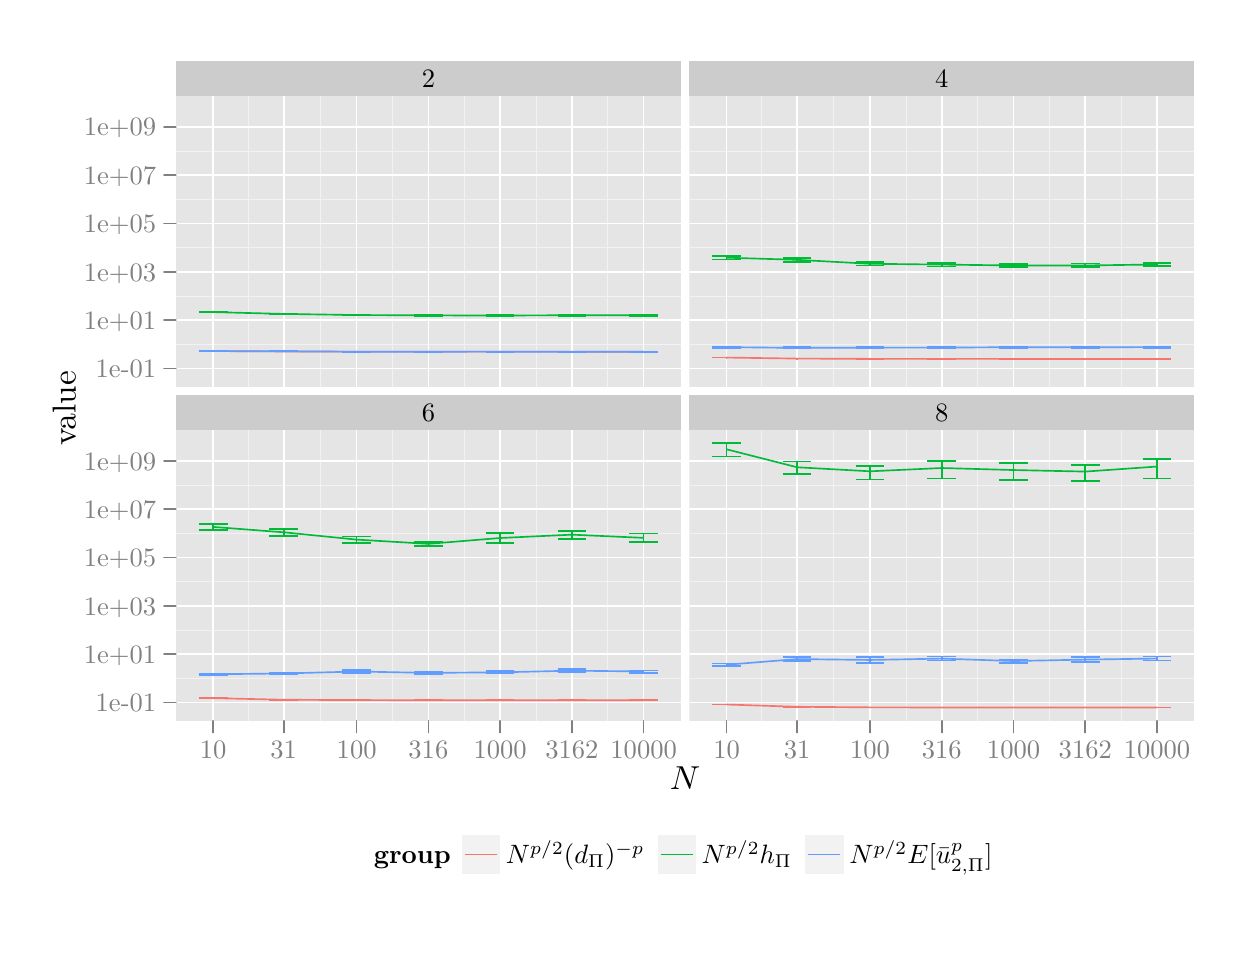
\begin{tikzpicture}[x=1pt,y=1pt]
\definecolor[named]{drawColor}{rgb}{0.00,0.00,0.00}
\definecolor[named]{fillColor}{rgb}{1.00,1.00,1.00}
\fill[color=fillColor,fill opacity=0.00,] (0,0) rectangle (433.62,325.21);
\begin{scope}
\path[clip] (  0.00,  0.00) rectangle (433.62,325.21);
\definecolor[named]{drawColor}{rgb}{0.41,0.16,0.58}
\end{scope}
\begin{scope}
\path[clip] (  0.00,  0.00) rectangle (433.62,325.21);
\definecolor[named]{drawColor}{rgb}{0.41,0.16,0.58}
\end{scope}
\begin{scope}
\path[clip] (  0.00,  0.00) rectangle (433.62,325.21);
\definecolor[named]{drawColor}{rgb}{0.41,0.16,0.58}
\end{scope}
\begin{scope}
\path[clip] (  0.00,  0.00) rectangle (433.62,325.21);
\definecolor[named]{drawColor}{rgb}{0.41,0.16,0.58}
\end{scope}
\begin{scope}
\path[clip] (  0.00,  0.00) rectangle (433.62,325.21);
\definecolor[named]{drawColor}{rgb}{0.41,0.16,0.58}
\end{scope}
\begin{scope}
\path[clip] (  0.00,  0.00) rectangle (433.62,325.21);
\definecolor[named]{drawColor}{rgb}{0.41,0.16,0.58}
\end{scope}
\begin{scope}
\path[clip] (  0.00,  0.00) rectangle (433.62,325.21);
\definecolor[named]{drawColor}{rgb}{0.41,0.16,0.58}
\end{scope}
\begin{scope}
\path[clip] (  0.00,  0.00) rectangle (433.62,325.21);
\definecolor[named]{drawColor}{rgb}{0.41,0.16,0.58}
\end{scope}
\begin{scope}
\path[clip] ( 53.55,195.47) rectangle (236.06,300.54);
\definecolor[named]{drawColor}{rgb}{0.41,0.16,0.58}
\end{scope}
\begin{scope}
\path[clip] (  0.00,  0.00) rectangle (433.62,325.21);
\definecolor[named]{drawColor}{rgb}{0.41,0.16,0.58}
\end{scope}
\begin{scope}
\path[clip] (239.07,195.47) rectangle (421.58,300.54);
\definecolor[named]{drawColor}{rgb}{0.41,0.16,0.58}
\end{scope}
\begin{scope}
\path[clip] (  0.00,  0.00) rectangle (433.62,325.21);
\definecolor[named]{drawColor}{rgb}{0.41,0.16,0.58}
\end{scope}
\begin{scope}
\path[clip] ( 53.55, 74.76) rectangle (236.06,179.83);
\definecolor[named]{drawColor}{rgb}{0.41,0.16,0.58}
\end{scope}
\begin{scope}
\path[clip] (  0.00,  0.00) rectangle (433.62,325.21);
\definecolor[named]{drawColor}{rgb}{0.41,0.16,0.58}
\end{scope}
\begin{scope}
\path[clip] (239.07, 74.76) rectangle (421.58,179.83);
\definecolor[named]{drawColor}{rgb}{0.41,0.16,0.58}
\end{scope}
\begin{scope}
\path[clip] (  0.00,  0.00) rectangle (433.62,325.21);
\definecolor[named]{drawColor}{rgb}{0.41,0.16,0.58}
\end{scope}
\begin{scope}
\path[clip] (  0.00,  0.00) rectangle (433.62,325.21);
\definecolor[named]{drawColor}{rgb}{0.41,0.16,0.58}
\end{scope}
\begin{scope}
\path[clip] (  0.00,  0.00) rectangle (433.62,325.21);
\definecolor[named]{drawColor}{rgb}{0.41,0.16,0.58}
\end{scope}
\begin{scope}
\path[clip] (  0.00,  0.00) rectangle (433.62,325.21);
\definecolor[named]{drawColor}{rgb}{0.41,0.16,0.58}
\end{scope}
\begin{scope}
\path[clip] (  0.00,  0.00) rectangle (433.62,325.21);
\definecolor[named]{drawColor}{rgb}{0.41,0.16,0.58}
\end{scope}
\begin{scope}
\path[clip] (  0.00,  0.00) rectangle (433.62,325.21);
\definecolor[named]{drawColor}{rgb}{0.41,0.16,0.58}
\end{scope}
\begin{scope}
\path[clip] (  0.00,  0.00) rectangle (433.62,325.21);
\definecolor[named]{drawColor}{rgb}{0.41,0.16,0.58}
\end{scope}
\begin{scope}
\path[clip] (  0.00,  0.00) rectangle (433.62,325.21);
\definecolor[named]{drawColor}{rgb}{0.41,0.16,0.58}
\end{scope}
\begin{scope}
\path[clip] (  0.00,  0.00) rectangle (433.62,325.21);
\definecolor[named]{drawColor}{rgb}{0.41,0.16,0.58}
\end{scope}
\begin{scope}
\path[clip] (  0.00,  0.00) rectangle (433.62,325.21);
\definecolor[named]{drawColor}{rgb}{0.41,0.16,0.58}
\end{scope}
\begin{scope}
\path[clip] (  0.00,  0.00) rectangle (433.62,325.21);
\definecolor[named]{drawColor}{rgb}{0.41,0.16,0.58}
\end{scope}
\begin{scope}
\path[clip] (  0.00,  0.00) rectangle (433.62,325.21);
\definecolor[named]{drawColor}{rgb}{0.41,0.16,0.58}
\end{scope}
\begin{scope}
\path[clip] (  0.00,  0.00) rectangle (433.62,325.21);
\definecolor[named]{drawColor}{rgb}{0.41,0.16,0.58}
\end{scope}
\begin{scope}
\path[clip] (  0.00,  0.00) rectangle (433.62,325.21);
\definecolor[named]{drawColor}{rgb}{0.41,0.16,0.58}
\end{scope}
\begin{scope}
\path[clip] (  0.00,  0.00) rectangle (433.62,325.21);
\definecolor[named]{drawColor}{rgb}{0.41,0.16,0.58}
\end{scope}
\begin{scope}
\path[clip] (  0.00,  0.00) rectangle (433.62,325.21);
\definecolor[named]{drawColor}{rgb}{0.41,0.16,0.58}
\end{scope}
\begin{scope}
\path[clip] (  0.00,  0.00) rectangle (433.62,325.21);
\definecolor[named]{drawColor}{rgb}{0.41,0.16,0.58}
\end{scope}
\begin{scope}
\path[clip] (  0.00,  0.00) rectangle (433.62,325.21);
\definecolor[named]{drawColor}{rgb}{0.41,0.16,0.58}
\end{scope}
\begin{scope}
\path[clip] (  0.00,  0.00) rectangle (433.62,325.21);
\definecolor[named]{drawColor}{rgb}{0.41,0.16,0.58}
\end{scope}
\begin{scope}
\path[clip] (  0.00,  0.00) rectangle (433.62,325.21);
\definecolor[named]{drawColor}{rgb}{0.41,0.16,0.58}
\end{scope}
\begin{scope}
\path[clip] (  0.00,  0.00) rectangle (433.62,325.21);
\definecolor[named]{drawColor}{rgb}{0.41,0.16,0.58}
\end{scope}
\begin{scope}
\path[clip] (  0.00,  0.00) rectangle (433.62,325.21);
\definecolor[named]{drawColor}{rgb}{0.41,0.16,0.58}
\end{scope}
\begin{scope}
\path[clip] (  0.00,  0.00) rectangle (433.62,325.21);
\definecolor[named]{drawColor}{rgb}{0.41,0.16,0.58}
\end{scope}
\begin{scope}
\path[clip] (  0.00,  0.00) rectangle (433.62,325.21);
\definecolor[named]{drawColor}{rgb}{0.41,0.16,0.58}
\end{scope}
\begin{scope}
\path[clip] (  0.00,  0.00) rectangle (433.62,325.21);
\definecolor[named]{drawColor}{rgb}{0.41,0.16,0.58}
\end{scope}
\begin{scope}
\path[clip] (  0.00,  0.00) rectangle (433.62,325.21);
\definecolor[named]{drawColor}{rgb}{0.41,0.16,0.58}
\end{scope}
\begin{scope}
\path[clip] (  0.00,  0.00) rectangle (433.62,325.21);
\definecolor[named]{drawColor}{rgb}{0.41,0.16,0.58}
\end{scope}
\begin{scope}
\path[clip] (  0.00,  0.00) rectangle (433.62,325.21);
\definecolor[named]{drawColor}{rgb}{0.41,0.16,0.58}
\end{scope}
\begin{scope}
\path[clip] (  0.00,  0.00) rectangle (433.62,325.21);
\definecolor[named]{drawColor}{rgb}{0.41,0.16,0.58}
\end{scope}
\begin{scope}
\path[clip] (  0.00,  0.00) rectangle (433.62,325.21);
\definecolor[named]{drawColor}{rgb}{0.41,0.16,0.58}
\end{scope}
\begin{scope}
\path[clip] (  0.00,  0.00) rectangle (433.62,325.21);
\definecolor[named]{drawColor}{rgb}{0.41,0.16,0.58}
\end{scope}
\begin{scope}
\path[clip] (  0.00,  0.00) rectangle (433.62,325.21);
\definecolor[named]{drawColor}{rgb}{0.41,0.16,0.58}
\end{scope}
\begin{scope}
\path[clip] (  0.00,  0.00) rectangle (433.62,325.21);
\definecolor[named]{drawColor}{rgb}{0.41,0.16,0.58}
\end{scope}
\begin{scope}
\path[clip] (  0.00,  0.00) rectangle (433.62,325.21);
\definecolor[named]{drawColor}{rgb}{0.41,0.16,0.58}
\definecolor[named]{fillColor}{rgb}{1.00,1.00,1.00}

\draw[fill=fillColor,draw opacity=0.00,] (  0.00,  0.00) rectangle (433.62,325.21);
\end{scope}
\begin{scope}
\path[clip] (  0.00,  0.00) rectangle (433.62,325.21);
\definecolor[named]{drawColor}{rgb}{0.41,0.16,0.58}
\end{scope}
\begin{scope}
\path[clip] ( 53.55,195.47) rectangle (236.06,300.54);
\definecolor[named]{drawColor}{rgb}{0.41,0.16,0.58}
\definecolor[named]{fillColor}{rgb}{0.90,0.90,0.90}

\draw[fill=fillColor,draw opacity=0.00,] ( 53.55,195.47) rectangle (236.06,300.54);
\definecolor[named]{drawColor}{rgb}{0.95,0.95,0.95}

\draw[color=drawColor,line width= 0.3pt,line cap=round,line join=round,fill opacity=0.00,] ( 53.55,210.76) --
	(236.06,210.76);

\draw[color=drawColor,line width= 0.3pt,line cap=round,line join=round,fill opacity=0.00,] ( 53.55,228.23) --
	(236.06,228.23);

\draw[color=drawColor,line width= 0.3pt,line cap=round,line join=round,fill opacity=0.00,] ( 53.55,245.70) --
	(236.06,245.70);

\draw[color=drawColor,line width= 0.3pt,line cap=round,line join=round,fill opacity=0.00,] ( 53.55,263.17) --
	(236.06,263.17);

\draw[color=drawColor,line width= 0.3pt,line cap=round,line join=round,fill opacity=0.00,] ( 53.55,280.64) --
	(236.06,280.64);

\draw[color=drawColor,line width= 0.3pt,line cap=round,line join=round,fill opacity=0.00,] ( 79.77,195.47) --
	( 79.77,300.54);

\draw[color=drawColor,line width= 0.3pt,line cap=round,line join=round,fill opacity=0.00,] (105.69,195.47) --
	(105.69,300.54);

\draw[color=drawColor,line width= 0.3pt,line cap=round,line join=round,fill opacity=0.00,] (131.83,195.47) --
	(131.83,300.54);

\draw[color=drawColor,line width= 0.3pt,line cap=round,line join=round,fill opacity=0.00,] (157.76,195.47) --
	(157.76,300.54);

\draw[color=drawColor,line width= 0.3pt,line cap=round,line join=round,fill opacity=0.00,] (183.69,195.47) --
	(183.69,300.54);

\draw[color=drawColor,line width= 0.3pt,line cap=round,line join=round,fill opacity=0.00,] (209.61,195.47) --
	(209.61,300.54);
\definecolor[named]{drawColor}{rgb}{1.00,1.00,1.00}

\draw[color=drawColor,line width= 0.6pt,line cap=round,line join=round,fill opacity=0.00,] ( 53.55,202.03) --
	(236.06,202.03);

\draw[color=drawColor,line width= 0.6pt,line cap=round,line join=round,fill opacity=0.00,] ( 53.55,219.50) --
	(236.06,219.50);

\draw[color=drawColor,line width= 0.6pt,line cap=round,line join=round,fill opacity=0.00,] ( 53.55,236.97) --
	(236.06,236.97);

\draw[color=drawColor,line width= 0.6pt,line cap=round,line join=round,fill opacity=0.00,] ( 53.55,254.44) --
	(236.06,254.44);

\draw[color=drawColor,line width= 0.6pt,line cap=round,line join=round,fill opacity=0.00,] ( 53.55,271.91) --
	(236.06,271.91);

\draw[color=drawColor,line width= 0.6pt,line cap=round,line join=round,fill opacity=0.00,] ( 53.55,289.38) --
	(236.06,289.38);

\draw[color=drawColor,line width= 0.6pt,line cap=round,line join=round,fill opacity=0.00,] ( 67.03,195.47) --
	( 67.03,300.54);

\draw[color=drawColor,line width= 0.6pt,line cap=round,line join=round,fill opacity=0.00,] ( 92.51,195.47) --
	( 92.51,300.54);

\draw[color=drawColor,line width= 0.6pt,line cap=round,line join=round,fill opacity=0.00,] (118.88,195.47) --
	(118.88,300.54);

\draw[color=drawColor,line width= 0.6pt,line cap=round,line join=round,fill opacity=0.00,] (144.79,195.47) --
	(144.79,300.54);

\draw[color=drawColor,line width= 0.6pt,line cap=round,line join=round,fill opacity=0.00,] (170.73,195.47) --
	(170.73,300.54);

\draw[color=drawColor,line width= 0.6pt,line cap=round,line join=round,fill opacity=0.00,] (196.65,195.47) --
	(196.65,300.54);

\draw[color=drawColor,line width= 0.6pt,line cap=round,line join=round,fill opacity=0.00,] (222.58,195.47) --
	(222.58,300.54);
\definecolor[named]{drawColor}{rgb}{0.97,0.46,0.43}

\draw[color=drawColor,line width= 0.6pt,line join=round,fill opacity=0.00,] ( 67.03,208.37) --
	( 92.51,208.20) --
	(118.88,208.15) --
	(144.79,208.14) --
	(170.73,208.14) --
	(196.65,208.13) --
	(222.58,208.13);
\definecolor[named]{drawColor}{rgb}{0.00,0.73,0.22}

\draw[color=drawColor,line width= 0.6pt,line join=round,fill opacity=0.00,] ( 67.03,222.43) --
	( 92.51,221.77) --
	(118.88,221.37) --
	(144.79,221.25) --
	(170.73,221.19) --
	(196.65,221.30) --
	(222.58,221.31);
\definecolor[named]{drawColor}{rgb}{0.38,0.61,1.00}

\draw[color=drawColor,line width= 0.6pt,line join=round,fill opacity=0.00,] ( 67.03,208.33) --
	( 92.51,208.25) --
	(118.88,208.12) --
	(144.79,208.12) --
	(170.73,208.14) --
	(196.65,208.07) --
	(222.58,208.14);
\definecolor[named]{drawColor}{rgb}{0.97,0.46,0.43}

\draw[color=drawColor,line width= 0.6pt,line join=round,fill opacity=0.00,] ( 61.85,208.37) --
	( 72.22,208.37);

\draw[color=drawColor,line width= 0.6pt,line join=round,fill opacity=0.00,] ( 67.03,208.37) --
	( 67.03,208.36);

\draw[color=drawColor,line width= 0.6pt,line join=round,fill opacity=0.00,] ( 61.85,208.36) --
	( 72.22,208.36);

\draw[color=drawColor,line width= 0.6pt,line join=round,fill opacity=0.00,] ( 87.32,208.20) --
	( 97.69,208.20);

\draw[color=drawColor,line width= 0.6pt,line join=round,fill opacity=0.00,] ( 92.51,208.20) --
	( 92.51,208.20);

\draw[color=drawColor,line width= 0.6pt,line join=round,fill opacity=0.00,] ( 87.32,208.20) --
	( 97.69,208.20);

\draw[color=drawColor,line width= 0.6pt,line join=round,fill opacity=0.00,] (113.69,208.15) --
	(124.06,208.15);

\draw[color=drawColor,line width= 0.6pt,line join=round,fill opacity=0.00,] (118.88,208.15) --
	(118.88,208.15);

\draw[color=drawColor,line width= 0.6pt,line join=round,fill opacity=0.00,] (113.69,208.15) --
	(124.06,208.15);

\draw[color=drawColor,line width= 0.6pt,line join=round,fill opacity=0.00,] (139.60,208.14) --
	(149.97,208.14);

\draw[color=drawColor,line width= 0.6pt,line join=round,fill opacity=0.00,] (144.79,208.14) --
	(144.79,208.14);

\draw[color=drawColor,line width= 0.6pt,line join=round,fill opacity=0.00,] (139.60,208.14) --
	(149.97,208.14);

\draw[color=drawColor,line width= 0.6pt,line join=round,fill opacity=0.00,] (165.54,208.14) --
	(175.91,208.14);

\draw[color=drawColor,line width= 0.6pt,line join=round,fill opacity=0.00,] (170.73,208.14) --
	(170.73,208.14);

\draw[color=drawColor,line width= 0.6pt,line join=round,fill opacity=0.00,] (165.54,208.14) --
	(175.91,208.14);

\draw[color=drawColor,line width= 0.6pt,line join=round,fill opacity=0.00,] (191.47,208.13) --
	(201.83,208.13);

\draw[color=drawColor,line width= 0.6pt,line join=round,fill opacity=0.00,] (196.65,208.13) --
	(196.65,208.13);

\draw[color=drawColor,line width= 0.6pt,line join=round,fill opacity=0.00,] (191.47,208.13) --
	(201.83,208.13);

\draw[color=drawColor,line width= 0.6pt,line join=round,fill opacity=0.00,] (217.39,208.13) --
	(227.76,208.13);

\draw[color=drawColor,line width= 0.6pt,line join=round,fill opacity=0.00,] (222.58,208.13) --
	(222.58,208.13);

\draw[color=drawColor,line width= 0.6pt,line join=round,fill opacity=0.00,] (217.39,208.13) --
	(227.76,208.13);
\definecolor[named]{drawColor}{rgb}{0.00,0.73,0.22}

\draw[color=drawColor,line width= 0.6pt,line join=round,fill opacity=0.00,] ( 61.85,222.60) --
	( 72.22,222.60);

\draw[color=drawColor,line width= 0.6pt,line join=round,fill opacity=0.00,] ( 67.03,222.60) --
	( 67.03,222.24);

\draw[color=drawColor,line width= 0.6pt,line join=round,fill opacity=0.00,] ( 61.85,222.24) --
	( 72.22,222.24);

\draw[color=drawColor,line width= 0.6pt,line join=round,fill opacity=0.00,] ( 87.32,221.97) --
	( 97.69,221.97);

\draw[color=drawColor,line width= 0.6pt,line join=round,fill opacity=0.00,] ( 92.51,221.97) --
	( 92.51,221.57);

\draw[color=drawColor,line width= 0.6pt,line join=round,fill opacity=0.00,] ( 87.32,221.57) --
	( 97.69,221.57);

\draw[color=drawColor,line width= 0.6pt,line join=round,fill opacity=0.00,] (113.69,221.57) --
	(124.06,221.57);

\draw[color=drawColor,line width= 0.6pt,line join=round,fill opacity=0.00,] (118.88,221.57) --
	(118.88,221.17);

\draw[color=drawColor,line width= 0.6pt,line join=round,fill opacity=0.00,] (113.69,221.17) --
	(124.06,221.17);

\draw[color=drawColor,line width= 0.6pt,line join=round,fill opacity=0.00,] (139.60,221.44) --
	(149.97,221.44);

\draw[color=drawColor,line width= 0.6pt,line join=round,fill opacity=0.00,] (144.79,221.44) --
	(144.79,221.05);

\draw[color=drawColor,line width= 0.6pt,line join=round,fill opacity=0.00,] (139.60,221.05) --
	(149.97,221.05);

\draw[color=drawColor,line width= 0.6pt,line join=round,fill opacity=0.00,] (165.54,221.38) --
	(175.91,221.38);

\draw[color=drawColor,line width= 0.6pt,line join=round,fill opacity=0.00,] (170.73,221.38) --
	(170.73,220.99);

\draw[color=drawColor,line width= 0.6pt,line join=round,fill opacity=0.00,] (165.54,220.99) --
	(175.91,220.99);

\draw[color=drawColor,line width= 0.6pt,line join=round,fill opacity=0.00,] (191.47,221.51) --
	(201.83,221.51);

\draw[color=drawColor,line width= 0.6pt,line join=round,fill opacity=0.00,] (196.65,221.51) --
	(196.65,221.12);

\draw[color=drawColor,line width= 0.6pt,line join=round,fill opacity=0.00,] (191.47,221.12) --
	(201.83,221.12);

\draw[color=drawColor,line width= 0.6pt,line join=round,fill opacity=0.00,] (217.39,221.51) --
	(227.76,221.51);

\draw[color=drawColor,line width= 0.6pt,line join=round,fill opacity=0.00,] (222.58,221.51) --
	(222.58,221.12);

\draw[color=drawColor,line width= 0.6pt,line join=round,fill opacity=0.00,] (217.39,221.12) --
	(227.76,221.12);
\definecolor[named]{drawColor}{rgb}{0.38,0.61,1.00}

\draw[color=drawColor,line width= 0.6pt,line join=round,fill opacity=0.00,] ( 61.85,208.43) --
	( 72.22,208.43);

\draw[color=drawColor,line width= 0.6pt,line join=round,fill opacity=0.00,] ( 67.03,208.43) --
	( 67.03,208.24);

\draw[color=drawColor,line width= 0.6pt,line join=round,fill opacity=0.00,] ( 61.85,208.24) --
	( 72.22,208.24);

\draw[color=drawColor,line width= 0.6pt,line join=round,fill opacity=0.00,] ( 87.32,208.36) --
	( 97.69,208.36);

\draw[color=drawColor,line width= 0.6pt,line join=round,fill opacity=0.00,] ( 92.51,208.36) --
	( 92.51,208.16);

\draw[color=drawColor,line width= 0.6pt,line join=round,fill opacity=0.00,] ( 87.32,208.16) --
	( 97.69,208.16);

\draw[color=drawColor,line width= 0.6pt,line join=round,fill opacity=0.00,] (113.69,208.22) --
	(124.06,208.22);

\draw[color=drawColor,line width= 0.6pt,line join=round,fill opacity=0.00,] (118.88,208.22) --
	(118.88,208.01);

\draw[color=drawColor,line width= 0.6pt,line join=round,fill opacity=0.00,] (113.69,208.01) --
	(124.06,208.01);

\draw[color=drawColor,line width= 0.6pt,line join=round,fill opacity=0.00,] (139.60,208.23) --
	(149.97,208.23);

\draw[color=drawColor,line width= 0.6pt,line join=round,fill opacity=0.00,] (144.79,208.23) --
	(144.79,208.01);

\draw[color=drawColor,line width= 0.6pt,line join=round,fill opacity=0.00,] (139.60,208.01) --
	(149.97,208.01);

\draw[color=drawColor,line width= 0.6pt,line join=round,fill opacity=0.00,] (165.54,208.25) --
	(175.91,208.25);

\draw[color=drawColor,line width= 0.6pt,line join=round,fill opacity=0.00,] (170.73,208.25) --
	(170.73,208.04);

\draw[color=drawColor,line width= 0.6pt,line join=round,fill opacity=0.00,] (165.54,208.04) --
	(175.91,208.04);

\draw[color=drawColor,line width= 0.6pt,line join=round,fill opacity=0.00,] (191.47,208.17) --
	(201.83,208.17);

\draw[color=drawColor,line width= 0.6pt,line join=round,fill opacity=0.00,] (196.65,208.17) --
	(196.65,207.97);

\draw[color=drawColor,line width= 0.6pt,line join=round,fill opacity=0.00,] (191.47,207.97) --
	(201.83,207.97);

\draw[color=drawColor,line width= 0.6pt,line join=round,fill opacity=0.00,] (217.39,208.25) --
	(227.76,208.25);

\draw[color=drawColor,line width= 0.6pt,line join=round,fill opacity=0.00,] (222.58,208.25) --
	(222.58,208.03);

\draw[color=drawColor,line width= 0.6pt,line join=round,fill opacity=0.00,] (217.39,208.03) --
	(227.76,208.03);
\end{scope}
\begin{scope}
\path[clip] (  0.00,  0.00) rectangle (433.62,325.21);
\definecolor[named]{drawColor}{rgb}{0.41,0.16,0.58}
\end{scope}
\begin{scope}
\path[clip] (239.07,195.47) rectangle (421.58,300.54);
\definecolor[named]{drawColor}{rgb}{0.41,0.16,0.58}
\definecolor[named]{fillColor}{rgb}{0.90,0.90,0.90}

\draw[fill=fillColor,draw opacity=0.00,] (239.07,195.47) rectangle (421.57,300.54);
\definecolor[named]{drawColor}{rgb}{0.95,0.95,0.95}

\draw[color=drawColor,line width= 0.3pt,line cap=round,line join=round,fill opacity=0.00,] (239.07,210.76) --
	(421.58,210.76);

\draw[color=drawColor,line width= 0.3pt,line cap=round,line join=round,fill opacity=0.00,] (239.07,228.23) --
	(421.58,228.23);

\draw[color=drawColor,line width= 0.3pt,line cap=round,line join=round,fill opacity=0.00,] (239.07,245.70) --
	(421.58,245.70);

\draw[color=drawColor,line width= 0.3pt,line cap=round,line join=round,fill opacity=0.00,] (239.07,263.17) --
	(421.58,263.17);

\draw[color=drawColor,line width= 0.3pt,line cap=round,line join=round,fill opacity=0.00,] (239.07,280.64) --
	(421.58,280.64);

\draw[color=drawColor,line width= 0.3pt,line cap=round,line join=round,fill opacity=0.00,] (265.29,195.47) --
	(265.29,300.54);

\draw[color=drawColor,line width= 0.3pt,line cap=round,line join=round,fill opacity=0.00,] (291.21,195.47) --
	(291.21,300.54);

\draw[color=drawColor,line width= 0.3pt,line cap=round,line join=round,fill opacity=0.00,] (317.35,195.47) --
	(317.35,300.54);

\draw[color=drawColor,line width= 0.3pt,line cap=round,line join=round,fill opacity=0.00,] (343.28,195.47) --
	(343.28,300.54);

\draw[color=drawColor,line width= 0.3pt,line cap=round,line join=round,fill opacity=0.00,] (369.21,195.47) --
	(369.21,300.54);

\draw[color=drawColor,line width= 0.3pt,line cap=round,line join=round,fill opacity=0.00,] (395.13,195.47) --
	(395.13,300.54);
\definecolor[named]{drawColor}{rgb}{1.00,1.00,1.00}

\draw[color=drawColor,line width= 0.6pt,line cap=round,line join=round,fill opacity=0.00,] (239.07,202.03) --
	(421.58,202.03);

\draw[color=drawColor,line width= 0.6pt,line cap=round,line join=round,fill opacity=0.00,] (239.07,219.50) --
	(421.58,219.50);

\draw[color=drawColor,line width= 0.6pt,line cap=round,line join=round,fill opacity=0.00,] (239.07,236.97) --
	(421.58,236.97);

\draw[color=drawColor,line width= 0.6pt,line cap=round,line join=round,fill opacity=0.00,] (239.07,254.44) --
	(421.58,254.44);

\draw[color=drawColor,line width= 0.6pt,line cap=round,line join=round,fill opacity=0.00,] (239.07,271.91) --
	(421.58,271.91);

\draw[color=drawColor,line width= 0.6pt,line cap=round,line join=round,fill opacity=0.00,] (239.07,289.38) --
	(421.58,289.38);

\draw[color=drawColor,line width= 0.6pt,line cap=round,line join=round,fill opacity=0.00,] (252.55,195.47) --
	(252.55,300.54);

\draw[color=drawColor,line width= 0.6pt,line cap=round,line join=round,fill opacity=0.00,] (278.03,195.47) --
	(278.03,300.54);

\draw[color=drawColor,line width= 0.6pt,line cap=round,line join=round,fill opacity=0.00,] (304.40,195.47) --
	(304.40,300.54);

\draw[color=drawColor,line width= 0.6pt,line cap=round,line join=round,fill opacity=0.00,] (330.31,195.47) --
	(330.31,300.54);

\draw[color=drawColor,line width= 0.6pt,line cap=round,line join=round,fill opacity=0.00,] (356.25,195.47) --
	(356.25,300.54);

\draw[color=drawColor,line width= 0.6pt,line cap=round,line join=round,fill opacity=0.00,] (382.17,195.47) --
	(382.17,300.54);

\draw[color=drawColor,line width= 0.6pt,line cap=round,line join=round,fill opacity=0.00,] (408.09,195.47) --
	(408.09,300.54);
\definecolor[named]{drawColor}{rgb}{0.97,0.46,0.43}

\draw[color=drawColor,line width= 0.6pt,line join=round,fill opacity=0.00,] (252.55,206.00) --
	(278.03,205.63) --
	(304.40,205.54) --
	(330.31,205.52) --
	(356.25,205.51) --
	(382.17,205.51) --
	(408.09,205.50);
\definecolor[named]{drawColor}{rgb}{0.00,0.73,0.22}

\draw[color=drawColor,line width= 0.6pt,line join=round,fill opacity=0.00,] (252.55,242.09) --
	(278.03,241.32) --
	(304.40,239.89) --
	(330.31,239.60) --
	(356.25,239.28) --
	(382.17,239.28) --
	(408.09,239.64);
\definecolor[named]{drawColor}{rgb}{0.38,0.61,1.00}

\draw[color=drawColor,line width= 0.6pt,line join=round,fill opacity=0.00,] (252.55,209.76) --
	(278.03,209.50) --
	(304.40,209.59) --
	(330.31,209.59) --
	(356.25,209.76) --
	(382.17,209.69) --
	(408.09,209.79);
\definecolor[named]{drawColor}{rgb}{0.97,0.46,0.43}

\draw[color=drawColor,line width= 0.6pt,line join=round,fill opacity=0.00,] (247.36,206.02) --
	(257.73,206.02);

\draw[color=drawColor,line width= 0.6pt,line join=round,fill opacity=0.00,] (252.55,206.02) --
	(252.55,205.98);

\draw[color=drawColor,line width= 0.6pt,line join=round,fill opacity=0.00,] (247.36,205.98) --
	(257.73,205.98);

\draw[color=drawColor,line width= 0.6pt,line join=round,fill opacity=0.00,] (272.84,205.64) --
	(283.21,205.64);

\draw[color=drawColor,line width= 0.6pt,line join=round,fill opacity=0.00,] (278.03,205.64) --
	(278.03,205.63);

\draw[color=drawColor,line width= 0.6pt,line join=round,fill opacity=0.00,] (272.84,205.63) --
	(283.21,205.63);

\draw[color=drawColor,line width= 0.6pt,line join=round,fill opacity=0.00,] (299.21,205.54) --
	(309.58,205.54);

\draw[color=drawColor,line width= 0.6pt,line join=round,fill opacity=0.00,] (304.40,205.54) --
	(304.40,205.54);

\draw[color=drawColor,line width= 0.6pt,line join=round,fill opacity=0.00,] (299.21,205.54) --
	(309.58,205.54);

\draw[color=drawColor,line width= 0.6pt,line join=round,fill opacity=0.00,] (325.12,205.52) --
	(335.49,205.52);

\draw[color=drawColor,line width= 0.6pt,line join=round,fill opacity=0.00,] (330.31,205.52) --
	(330.31,205.52);

\draw[color=drawColor,line width= 0.6pt,line join=round,fill opacity=0.00,] (325.12,205.52) --
	(335.49,205.52);

\draw[color=drawColor,line width= 0.6pt,line join=round,fill opacity=0.00,] (351.06,205.51) --
	(361.43,205.51);

\draw[color=drawColor,line width= 0.6pt,line join=round,fill opacity=0.00,] (356.25,205.51) --
	(356.25,205.51);

\draw[color=drawColor,line width= 0.6pt,line join=round,fill opacity=0.00,] (351.06,205.51) --
	(361.43,205.51);

\draw[color=drawColor,line width= 0.6pt,line join=round,fill opacity=0.00,] (376.98,205.51) --
	(387.35,205.51);

\draw[color=drawColor,line width= 0.6pt,line join=round,fill opacity=0.00,] (382.17,205.51) --
	(382.17,205.51);

\draw[color=drawColor,line width= 0.6pt,line join=round,fill opacity=0.00,] (376.98,205.51) --
	(387.35,205.51);

\draw[color=drawColor,line width= 0.6pt,line join=round,fill opacity=0.00,] (402.91,205.50) --
	(413.28,205.50);

\draw[color=drawColor,line width= 0.6pt,line join=round,fill opacity=0.00,] (408.09,205.50) --
	(408.09,205.50);

\draw[color=drawColor,line width= 0.6pt,line join=round,fill opacity=0.00,] (402.91,205.50) --
	(413.28,205.50);
\definecolor[named]{drawColor}{rgb}{0.00,0.73,0.22}

\draw[color=drawColor,line width= 0.6pt,line join=round,fill opacity=0.00,] (247.36,242.67) --
	(257.73,242.67);

\draw[color=drawColor,line width= 0.6pt,line join=round,fill opacity=0.00,] (252.55,242.67) --
	(252.55,241.48);

\draw[color=drawColor,line width= 0.6pt,line join=round,fill opacity=0.00,] (247.36,241.48) --
	(257.73,241.48);

\draw[color=drawColor,line width= 0.6pt,line join=round,fill opacity=0.00,] (272.84,241.97) --
	(283.21,241.97);

\draw[color=drawColor,line width= 0.6pt,line join=round,fill opacity=0.00,] (278.03,241.97) --
	(278.03,240.59);

\draw[color=drawColor,line width= 0.6pt,line join=round,fill opacity=0.00,] (272.84,240.59) --
	(283.21,240.59);

\draw[color=drawColor,line width= 0.6pt,line join=round,fill opacity=0.00,] (299.21,240.50) --
	(309.58,240.50);

\draw[color=drawColor,line width= 0.6pt,line join=round,fill opacity=0.00,] (304.40,240.50) --
	(304.40,239.24);

\draw[color=drawColor,line width= 0.6pt,line join=round,fill opacity=0.00,] (299.21,239.24) --
	(309.58,239.24);

\draw[color=drawColor,line width= 0.6pt,line join=round,fill opacity=0.00,] (325.12,240.29) --
	(335.49,240.29);

\draw[color=drawColor,line width= 0.6pt,line join=round,fill opacity=0.00,] (330.31,240.29) --
	(330.31,238.89);

\draw[color=drawColor,line width= 0.6pt,line join=round,fill opacity=0.00,] (325.12,238.89) --
	(335.49,238.89);

\draw[color=drawColor,line width= 0.6pt,line join=round,fill opacity=0.00,] (351.06,239.79) --
	(361.43,239.79);

\draw[color=drawColor,line width= 0.6pt,line join=round,fill opacity=0.00,] (356.25,239.79) --
	(356.25,238.70);

\draw[color=drawColor,line width= 0.6pt,line join=round,fill opacity=0.00,] (351.06,238.70) --
	(361.43,238.70);

\draw[color=drawColor,line width= 0.6pt,line join=round,fill opacity=0.00,] (376.98,239.93) --
	(387.35,239.93);

\draw[color=drawColor,line width= 0.6pt,line join=round,fill opacity=0.00,] (382.17,239.93) --
	(382.17,238.62);

\draw[color=drawColor,line width= 0.6pt,line join=round,fill opacity=0.00,] (376.98,238.62) --
	(387.35,238.62);

\draw[color=drawColor,line width= 0.6pt,line join=round,fill opacity=0.00,] (402.91,240.24) --
	(413.28,240.24);

\draw[color=drawColor,line width= 0.6pt,line join=round,fill opacity=0.00,] (408.09,240.24) --
	(408.09,239.07);

\draw[color=drawColor,line width= 0.6pt,line join=round,fill opacity=0.00,] (402.91,239.07) --
	(413.28,239.07);
\definecolor[named]{drawColor}{rgb}{0.38,0.61,1.00}

\draw[color=drawColor,line width= 0.6pt,line join=round,fill opacity=0.00,] (247.36,209.96) --
	(257.73,209.96);

\draw[color=drawColor,line width= 0.6pt,line join=round,fill opacity=0.00,] (252.55,209.96) --
	(252.55,209.56);

\draw[color=drawColor,line width= 0.6pt,line join=round,fill opacity=0.00,] (247.36,209.56) --
	(257.73,209.56);

\draw[color=drawColor,line width= 0.6pt,line join=round,fill opacity=0.00,] (272.84,209.71) --
	(283.21,209.71);

\draw[color=drawColor,line width= 0.6pt,line join=round,fill opacity=0.00,] (278.03,209.71) --
	(278.03,209.24);

\draw[color=drawColor,line width= 0.6pt,line join=round,fill opacity=0.00,] (272.84,209.24) --
	(283.21,209.24);

\draw[color=drawColor,line width= 0.6pt,line join=round,fill opacity=0.00,] (299.21,209.83) --
	(309.58,209.83);

\draw[color=drawColor,line width= 0.6pt,line join=round,fill opacity=0.00,] (304.40,209.83) --
	(304.40,209.35);

\draw[color=drawColor,line width= 0.6pt,line join=round,fill opacity=0.00,] (299.21,209.35) --
	(309.58,209.35);

\draw[color=drawColor,line width= 0.6pt,line join=round,fill opacity=0.00,] (325.12,209.83) --
	(335.49,209.83);

\draw[color=drawColor,line width= 0.6pt,line join=round,fill opacity=0.00,] (330.31,209.83) --
	(330.31,209.35);

\draw[color=drawColor,line width= 0.6pt,line join=round,fill opacity=0.00,] (325.12,209.35) --
	(335.49,209.35);

\draw[color=drawColor,line width= 0.6pt,line join=round,fill opacity=0.00,] (351.06,209.99) --
	(361.43,209.99);

\draw[color=drawColor,line width= 0.6pt,line join=round,fill opacity=0.00,] (356.25,209.99) --
	(356.25,209.52);

\draw[color=drawColor,line width= 0.6pt,line join=round,fill opacity=0.00,] (351.06,209.52) --
	(361.43,209.52);

\draw[color=drawColor,line width= 0.6pt,line join=round,fill opacity=0.00,] (376.98,209.93) --
	(387.35,209.93);

\draw[color=drawColor,line width= 0.6pt,line join=round,fill opacity=0.00,] (382.17,209.93) --
	(382.17,209.44);

\draw[color=drawColor,line width= 0.6pt,line join=round,fill opacity=0.00,] (376.98,209.44) --
	(387.35,209.44);

\draw[color=drawColor,line width= 0.6pt,line join=round,fill opacity=0.00,] (402.91,210.01) --
	(413.28,210.01);

\draw[color=drawColor,line width= 0.6pt,line join=round,fill opacity=0.00,] (408.09,210.01) --
	(408.09,209.52);

\draw[color=drawColor,line width= 0.6pt,line join=round,fill opacity=0.00,] (402.91,209.52) --
	(413.28,209.52);
\end{scope}
\begin{scope}
\path[clip] (  0.00,  0.00) rectangle (433.62,325.21);
\definecolor[named]{drawColor}{rgb}{0.41,0.16,0.58}
\end{scope}
\begin{scope}
\path[clip] ( 53.55, 74.76) rectangle (236.06,179.83);
\definecolor[named]{drawColor}{rgb}{0.41,0.16,0.58}
\definecolor[named]{fillColor}{rgb}{0.90,0.90,0.90}

\draw[fill=fillColor,draw opacity=0.00,] ( 53.55, 74.76) rectangle (236.06,179.83);
\definecolor[named]{drawColor}{rgb}{0.95,0.95,0.95}

\draw[color=drawColor,line width= 0.3pt,line cap=round,line join=round,fill opacity=0.00,] ( 53.55, 90.05) --
	(236.06, 90.05);

\draw[color=drawColor,line width= 0.3pt,line cap=round,line join=round,fill opacity=0.00,] ( 53.55,107.52) --
	(236.06,107.52);

\draw[color=drawColor,line width= 0.3pt,line cap=round,line join=round,fill opacity=0.00,] ( 53.55,124.99) --
	(236.06,124.99);

\draw[color=drawColor,line width= 0.3pt,line cap=round,line join=round,fill opacity=0.00,] ( 53.55,142.46) --
	(236.06,142.46);

\draw[color=drawColor,line width= 0.3pt,line cap=round,line join=round,fill opacity=0.00,] ( 53.55,159.93) --
	(236.06,159.93);

\draw[color=drawColor,line width= 0.3pt,line cap=round,line join=round,fill opacity=0.00,] ( 79.77, 74.76) --
	( 79.77,179.83);

\draw[color=drawColor,line width= 0.3pt,line cap=round,line join=round,fill opacity=0.00,] (105.69, 74.76) --
	(105.69,179.83);

\draw[color=drawColor,line width= 0.3pt,line cap=round,line join=round,fill opacity=0.00,] (131.83, 74.76) --
	(131.83,179.83);

\draw[color=drawColor,line width= 0.3pt,line cap=round,line join=round,fill opacity=0.00,] (157.76, 74.76) --
	(157.76,179.83);

\draw[color=drawColor,line width= 0.3pt,line cap=round,line join=round,fill opacity=0.00,] (183.69, 74.76) --
	(183.69,179.83);

\draw[color=drawColor,line width= 0.3pt,line cap=round,line join=round,fill opacity=0.00,] (209.61, 74.76) --
	(209.61,179.83);
\definecolor[named]{drawColor}{rgb}{1.00,1.00,1.00}

\draw[color=drawColor,line width= 0.6pt,line cap=round,line join=round,fill opacity=0.00,] ( 53.55, 81.32) --
	(236.06, 81.32);

\draw[color=drawColor,line width= 0.6pt,line cap=round,line join=round,fill opacity=0.00,] ( 53.55, 98.79) --
	(236.06, 98.79);

\draw[color=drawColor,line width= 0.6pt,line cap=round,line join=round,fill opacity=0.00,] ( 53.55,116.26) --
	(236.06,116.26);

\draw[color=drawColor,line width= 0.6pt,line cap=round,line join=round,fill opacity=0.00,] ( 53.55,133.73) --
	(236.06,133.73);

\draw[color=drawColor,line width= 0.6pt,line cap=round,line join=round,fill opacity=0.00,] ( 53.55,151.20) --
	(236.06,151.20);

\draw[color=drawColor,line width= 0.6pt,line cap=round,line join=round,fill opacity=0.00,] ( 53.55,168.67) --
	(236.06,168.67);

\draw[color=drawColor,line width= 0.6pt,line cap=round,line join=round,fill opacity=0.00,] ( 67.03, 74.76) --
	( 67.03,179.83);

\draw[color=drawColor,line width= 0.6pt,line cap=round,line join=round,fill opacity=0.00,] ( 92.51, 74.76) --
	( 92.51,179.83);

\draw[color=drawColor,line width= 0.6pt,line cap=round,line join=round,fill opacity=0.00,] (118.88, 74.76) --
	(118.88,179.83);

\draw[color=drawColor,line width= 0.6pt,line cap=round,line join=round,fill opacity=0.00,] (144.79, 74.76) --
	(144.79,179.83);

\draw[color=drawColor,line width= 0.6pt,line cap=round,line join=round,fill opacity=0.00,] (170.73, 74.76) --
	(170.73,179.83);

\draw[color=drawColor,line width= 0.6pt,line cap=round,line join=round,fill opacity=0.00,] (196.65, 74.76) --
	(196.65,179.83);

\draw[color=drawColor,line width= 0.6pt,line cap=round,line join=round,fill opacity=0.00,] (222.58, 74.76) --
	(222.58,179.83);
\definecolor[named]{drawColor}{rgb}{0.97,0.46,0.43}

\draw[color=drawColor,line width= 0.6pt,line join=round,fill opacity=0.00,] ( 67.03, 82.93) --
	( 92.51, 82.36) --
	(118.88, 82.22) --
	(144.79, 82.18) --
	(170.73, 82.17) --
	(196.65, 82.17) --
	(222.58, 82.16);
\definecolor[named]{drawColor}{rgb}{0.00,0.73,0.22}

\draw[color=drawColor,line width= 0.6pt,line join=round,fill opacity=0.00,] ( 67.03,144.80) --
	( 92.51,142.86) --
	(118.88,140.22) --
	(144.79,138.69) --
	(170.73,140.80) --
	(196.65,142.01) --
	(222.58,140.85);
\definecolor[named]{drawColor}{rgb}{0.38,0.61,1.00}

\draw[color=drawColor,line width= 0.6pt,line join=round,fill opacity=0.00,] ( 67.03, 91.57) --
	( 92.51, 91.85) --
	(118.88, 92.56) --
	(144.79, 92.06) --
	(170.73, 92.26) --
	(196.65, 92.86) --
	(222.58, 92.57);
\definecolor[named]{drawColor}{rgb}{0.97,0.46,0.43}

\draw[color=drawColor,line width= 0.6pt,line join=round,fill opacity=0.00,] ( 61.85, 82.96) --
	( 72.22, 82.96);

\draw[color=drawColor,line width= 0.6pt,line join=round,fill opacity=0.00,] ( 67.03, 82.96) --
	( 67.03, 82.91);

\draw[color=drawColor,line width= 0.6pt,line join=round,fill opacity=0.00,] ( 61.85, 82.91) --
	( 72.22, 82.91);

\draw[color=drawColor,line width= 0.6pt,line join=round,fill opacity=0.00,] ( 87.32, 82.36) --
	( 97.69, 82.36);

\draw[color=drawColor,line width= 0.6pt,line join=round,fill opacity=0.00,] ( 92.51, 82.36) --
	( 92.51, 82.35);

\draw[color=drawColor,line width= 0.6pt,line join=round,fill opacity=0.00,] ( 87.32, 82.35) --
	( 97.69, 82.35);

\draw[color=drawColor,line width= 0.6pt,line join=round,fill opacity=0.00,] (113.69, 82.23) --
	(124.06, 82.23);

\draw[color=drawColor,line width= 0.6pt,line join=round,fill opacity=0.00,] (118.88, 82.23) --
	(118.88, 82.22);

\draw[color=drawColor,line width= 0.6pt,line join=round,fill opacity=0.00,] (113.69, 82.22) --
	(124.06, 82.22);

\draw[color=drawColor,line width= 0.6pt,line join=round,fill opacity=0.00,] (139.60, 82.18) --
	(149.97, 82.18);

\draw[color=drawColor,line width= 0.6pt,line join=round,fill opacity=0.00,] (144.79, 82.18) --
	(144.79, 82.18);

\draw[color=drawColor,line width= 0.6pt,line join=round,fill opacity=0.00,] (139.60, 82.18) --
	(149.97, 82.18);

\draw[color=drawColor,line width= 0.6pt,line join=round,fill opacity=0.00,] (165.54, 82.17) --
	(175.91, 82.17);

\draw[color=drawColor,line width= 0.6pt,line join=round,fill opacity=0.00,] (170.73, 82.17) --
	(170.73, 82.17);

\draw[color=drawColor,line width= 0.6pt,line join=round,fill opacity=0.00,] (165.54, 82.17) --
	(175.91, 82.17);

\draw[color=drawColor,line width= 0.6pt,line join=round,fill opacity=0.00,] (191.47, 82.17) --
	(201.83, 82.17);

\draw[color=drawColor,line width= 0.6pt,line join=round,fill opacity=0.00,] (196.65, 82.17) --
	(196.65, 82.17);

\draw[color=drawColor,line width= 0.6pt,line join=round,fill opacity=0.00,] (191.47, 82.17) --
	(201.83, 82.17);

\draw[color=drawColor,line width= 0.6pt,line join=round,fill opacity=0.00,] (217.39, 82.16) --
	(227.76, 82.16);

\draw[color=drawColor,line width= 0.6pt,line join=round,fill opacity=0.00,] (222.58, 82.16) --
	(222.58, 82.16);

\draw[color=drawColor,line width= 0.6pt,line join=round,fill opacity=0.00,] (217.39, 82.16) --
	(227.76, 82.16);
\definecolor[named]{drawColor}{rgb}{0.00,0.73,0.22}

\draw[color=drawColor,line width= 0.6pt,line join=round,fill opacity=0.00,] ( 61.85,145.85) --
	( 72.22,145.85);

\draw[color=drawColor,line width= 0.6pt,line join=round,fill opacity=0.00,] ( 67.03,145.85) --
	( 67.03,143.60);

\draw[color=drawColor,line width= 0.6pt,line join=round,fill opacity=0.00,] ( 61.85,143.60) --
	( 72.22,143.60);

\draw[color=drawColor,line width= 0.6pt,line join=round,fill opacity=0.00,] ( 87.32,144.13) --
	( 97.69,144.13);

\draw[color=drawColor,line width= 0.6pt,line join=round,fill opacity=0.00,] ( 92.51,144.13) --
	( 92.51,141.44);

\draw[color=drawColor,line width= 0.6pt,line join=round,fill opacity=0.00,] ( 87.32,141.44) --
	( 97.69,141.44);

\draw[color=drawColor,line width= 0.6pt,line join=round,fill opacity=0.00,] (113.69,141.36) --
	(124.06,141.36);

\draw[color=drawColor,line width= 0.6pt,line join=round,fill opacity=0.00,] (118.88,141.36) --
	(118.88,138.93);

\draw[color=drawColor,line width= 0.6pt,line join=round,fill opacity=0.00,] (113.69,138.93) --
	(124.06,138.93);

\draw[color=drawColor,line width= 0.6pt,line join=round,fill opacity=0.00,] (139.60,139.46) --
	(149.97,139.46);

\draw[color=drawColor,line width= 0.6pt,line join=round,fill opacity=0.00,] (144.79,139.46) --
	(144.79,137.83);

\draw[color=drawColor,line width= 0.6pt,line join=round,fill opacity=0.00,] (139.60,137.83) --
	(149.97,137.83);

\draw[color=drawColor,line width= 0.6pt,line join=round,fill opacity=0.00,] (165.54,142.62) --
	(175.91,142.62);

\draw[color=drawColor,line width= 0.6pt,line join=round,fill opacity=0.00,] (170.73,142.62) --
	(170.73,138.95);

\draw[color=drawColor,line width= 0.6pt,line join=round,fill opacity=0.00,] (165.54,138.95) --
	(175.91,138.95);

\draw[color=drawColor,line width= 0.6pt,line join=round,fill opacity=0.00,] (191.47,143.42) --
	(201.83,143.42);

\draw[color=drawColor,line width= 0.6pt,line join=round,fill opacity=0.00,] (196.65,143.42) --
	(196.65,140.48);

\draw[color=drawColor,line width= 0.6pt,line join=round,fill opacity=0.00,] (191.47,140.48) --
	(201.83,140.48);

\draw[color=drawColor,line width= 0.6pt,line join=round,fill opacity=0.00,] (217.39,142.38) --
	(227.76,142.38);

\draw[color=drawColor,line width= 0.6pt,line join=round,fill opacity=0.00,] (222.58,142.38) --
	(222.58,139.28);

\draw[color=drawColor,line width= 0.6pt,line join=round,fill opacity=0.00,] (217.39,139.28) --
	(227.76,139.28);
\definecolor[named]{drawColor}{rgb}{0.38,0.61,1.00}

\draw[color=drawColor,line width= 0.6pt,line join=round,fill opacity=0.00,] ( 61.85, 91.87) --
	( 72.22, 91.87);

\draw[color=drawColor,line width= 0.6pt,line join=round,fill opacity=0.00,] ( 67.03, 91.87) --
	( 67.03, 91.27);

\draw[color=drawColor,line width= 0.6pt,line join=round,fill opacity=0.00,] ( 61.85, 91.27) --
	( 72.22, 91.27);

\draw[color=drawColor,line width= 0.6pt,line join=round,fill opacity=0.00,] ( 87.32, 92.26) --
	( 97.69, 92.26);

\draw[color=drawColor,line width= 0.6pt,line join=round,fill opacity=0.00,] ( 92.51, 92.26) --
	( 92.51, 91.42);

\draw[color=drawColor,line width= 0.6pt,line join=round,fill opacity=0.00,] ( 87.32, 91.42) --
	( 97.69, 91.42);

\draw[color=drawColor,line width= 0.6pt,line join=round,fill opacity=0.00,] (113.69, 93.13) --
	(124.06, 93.13);

\draw[color=drawColor,line width= 0.6pt,line join=round,fill opacity=0.00,] (118.88, 93.13) --
	(118.88, 91.99);

\draw[color=drawColor,line width= 0.6pt,line join=round,fill opacity=0.00,] (113.69, 91.99) --
	(124.06, 91.99);

\draw[color=drawColor,line width= 0.6pt,line join=round,fill opacity=0.00,] (139.60, 92.55) --
	(149.97, 92.55);

\draw[color=drawColor,line width= 0.6pt,line join=round,fill opacity=0.00,] (144.79, 92.55) --
	(144.79, 91.55);

\draw[color=drawColor,line width= 0.6pt,line join=round,fill opacity=0.00,] (139.60, 91.55) --
	(149.97, 91.55);

\draw[color=drawColor,line width= 0.6pt,line join=round,fill opacity=0.00,] (165.54, 92.70) --
	(175.91, 92.70);

\draw[color=drawColor,line width= 0.6pt,line join=round,fill opacity=0.00,] (170.73, 92.70) --
	(170.73, 91.78);

\draw[color=drawColor,line width= 0.6pt,line join=round,fill opacity=0.00,] (165.54, 91.78) --
	(175.91, 91.78);

\draw[color=drawColor,line width= 0.6pt,line join=round,fill opacity=0.00,] (191.47, 93.38) --
	(201.83, 93.38);

\draw[color=drawColor,line width= 0.6pt,line join=round,fill opacity=0.00,] (196.65, 93.38) --
	(196.65, 92.35);

\draw[color=drawColor,line width= 0.6pt,line join=round,fill opacity=0.00,] (191.47, 92.35) --
	(201.83, 92.35);

\draw[color=drawColor,line width= 0.6pt,line join=round,fill opacity=0.00,] (217.39, 92.98) --
	(227.76, 92.98);

\draw[color=drawColor,line width= 0.6pt,line join=round,fill opacity=0.00,] (222.58, 92.98) --
	(222.58, 92.12);

\draw[color=drawColor,line width= 0.6pt,line join=round,fill opacity=0.00,] (217.39, 92.12) --
	(227.76, 92.12);
\end{scope}
\begin{scope}
\path[clip] (  0.00,  0.00) rectangle (433.62,325.21);
\definecolor[named]{drawColor}{rgb}{0.41,0.16,0.58}
\end{scope}
\begin{scope}
\path[clip] (239.07, 74.76) rectangle (421.58,179.83);
\definecolor[named]{drawColor}{rgb}{0.41,0.16,0.58}
\definecolor[named]{fillColor}{rgb}{0.90,0.90,0.90}

\draw[fill=fillColor,draw opacity=0.00,] (239.07, 74.76) rectangle (421.57,179.83);
\definecolor[named]{drawColor}{rgb}{0.95,0.95,0.95}

\draw[color=drawColor,line width= 0.3pt,line cap=round,line join=round,fill opacity=0.00,] (239.07, 90.05) --
	(421.58, 90.05);

\draw[color=drawColor,line width= 0.3pt,line cap=round,line join=round,fill opacity=0.00,] (239.07,107.52) --
	(421.58,107.52);

\draw[color=drawColor,line width= 0.3pt,line cap=round,line join=round,fill opacity=0.00,] (239.07,124.99) --
	(421.58,124.99);

\draw[color=drawColor,line width= 0.3pt,line cap=round,line join=round,fill opacity=0.00,] (239.07,142.46) --
	(421.58,142.46);

\draw[color=drawColor,line width= 0.3pt,line cap=round,line join=round,fill opacity=0.00,] (239.07,159.93) --
	(421.58,159.93);

\draw[color=drawColor,line width= 0.3pt,line cap=round,line join=round,fill opacity=0.00,] (265.29, 74.76) --
	(265.29,179.83);

\draw[color=drawColor,line width= 0.3pt,line cap=round,line join=round,fill opacity=0.00,] (291.21, 74.76) --
	(291.21,179.83);

\draw[color=drawColor,line width= 0.3pt,line cap=round,line join=round,fill opacity=0.00,] (317.35, 74.76) --
	(317.35,179.83);

\draw[color=drawColor,line width= 0.3pt,line cap=round,line join=round,fill opacity=0.00,] (343.28, 74.76) --
	(343.28,179.83);

\draw[color=drawColor,line width= 0.3pt,line cap=round,line join=round,fill opacity=0.00,] (369.21, 74.76) --
	(369.21,179.83);

\draw[color=drawColor,line width= 0.3pt,line cap=round,line join=round,fill opacity=0.00,] (395.13, 74.76) --
	(395.13,179.83);
\definecolor[named]{drawColor}{rgb}{1.00,1.00,1.00}

\draw[color=drawColor,line width= 0.6pt,line cap=round,line join=round,fill opacity=0.00,] (239.07, 81.32) --
	(421.58, 81.32);

\draw[color=drawColor,line width= 0.6pt,line cap=round,line join=round,fill opacity=0.00,] (239.07, 98.79) --
	(421.58, 98.79);

\draw[color=drawColor,line width= 0.6pt,line cap=round,line join=round,fill opacity=0.00,] (239.07,116.26) --
	(421.58,116.26);

\draw[color=drawColor,line width= 0.6pt,line cap=round,line join=round,fill opacity=0.00,] (239.07,133.73) --
	(421.58,133.73);

\draw[color=drawColor,line width= 0.6pt,line cap=round,line join=round,fill opacity=0.00,] (239.07,151.20) --
	(421.58,151.20);

\draw[color=drawColor,line width= 0.6pt,line cap=round,line join=round,fill opacity=0.00,] (239.07,168.67) --
	(421.58,168.67);

\draw[color=drawColor,line width= 0.6pt,line cap=round,line join=round,fill opacity=0.00,] (252.55, 74.76) --
	(252.55,179.83);

\draw[color=drawColor,line width= 0.6pt,line cap=round,line join=round,fill opacity=0.00,] (278.03, 74.76) --
	(278.03,179.83);

\draw[color=drawColor,line width= 0.6pt,line cap=round,line join=round,fill opacity=0.00,] (304.40, 74.76) --
	(304.40,179.83);

\draw[color=drawColor,line width= 0.6pt,line cap=round,line join=round,fill opacity=0.00,] (330.31, 74.76) --
	(330.31,179.83);

\draw[color=drawColor,line width= 0.6pt,line cap=round,line join=round,fill opacity=0.00,] (356.25, 74.76) --
	(356.25,179.83);

\draw[color=drawColor,line width= 0.6pt,line cap=round,line join=round,fill opacity=0.00,] (382.17, 74.76) --
	(382.17,179.83);

\draw[color=drawColor,line width= 0.6pt,line cap=round,line join=round,fill opacity=0.00,] (408.09, 74.76) --
	(408.09,179.83);
\definecolor[named]{drawColor}{rgb}{0.97,0.46,0.43}

\draw[color=drawColor,line width= 0.6pt,line join=round,fill opacity=0.00,] (252.55, 80.63) --
	(278.03, 79.81) --
	(304.40, 79.61) --
	(330.31, 79.56) --
	(356.25, 79.54) --
	(382.17, 79.54) --
	(408.09, 79.54);
\definecolor[named]{drawColor}{rgb}{0.00,0.73,0.22}

\draw[color=drawColor,line width= 0.6pt,line join=round,fill opacity=0.00,] (252.55,172.85) --
	(278.03,166.36) --
	(304.40,164.90) --
	(330.31,166.09) --
	(356.25,165.36) --
	(382.17,164.80) --
	(408.09,166.62);
\definecolor[named]{drawColor}{rgb}{0.38,0.61,1.00}

\draw[color=drawColor,line width= 0.6pt,line join=round,fill opacity=0.00,] (252.55, 95.01) --
	(278.03, 97.05) --
	(304.40, 96.73) --
	(330.31, 97.22) --
	(356.25, 96.34) --
	(382.17, 96.86) --
	(408.09, 97.24);
\definecolor[named]{drawColor}{rgb}{0.97,0.46,0.43}

\draw[color=drawColor,line width= 0.6pt,line join=round,fill opacity=0.00,] (247.36, 80.68) --
	(257.73, 80.68);

\draw[color=drawColor,line width= 0.6pt,line join=round,fill opacity=0.00,] (252.55, 80.68) --
	(252.55, 80.60);

\draw[color=drawColor,line width= 0.6pt,line join=round,fill opacity=0.00,] (247.36, 80.60) --
	(257.73, 80.60);

\draw[color=drawColor,line width= 0.6pt,line join=round,fill opacity=0.00,] (272.84, 79.82) --
	(283.21, 79.82);

\draw[color=drawColor,line width= 0.6pt,line join=round,fill opacity=0.00,] (278.03, 79.82) --
	(278.03, 79.80);

\draw[color=drawColor,line width= 0.6pt,line join=round,fill opacity=0.00,] (272.84, 79.80) --
	(283.21, 79.80);

\draw[color=drawColor,line width= 0.6pt,line join=round,fill opacity=0.00,] (299.21, 79.61) --
	(309.58, 79.61);

\draw[color=drawColor,line width= 0.6pt,line join=round,fill opacity=0.00,] (304.40, 79.61) --
	(304.40, 79.61);

\draw[color=drawColor,line width= 0.6pt,line join=round,fill opacity=0.00,] (299.21, 79.61) --
	(309.58, 79.61);

\draw[color=drawColor,line width= 0.6pt,line join=round,fill opacity=0.00,] (325.12, 79.56) --
	(335.49, 79.56);

\draw[color=drawColor,line width= 0.6pt,line join=round,fill opacity=0.00,] (330.31, 79.56) --
	(330.31, 79.56);

\draw[color=drawColor,line width= 0.6pt,line join=round,fill opacity=0.00,] (325.12, 79.56) --
	(335.49, 79.56);

\draw[color=drawColor,line width= 0.6pt,line join=round,fill opacity=0.00,] (351.06, 79.54) --
	(361.43, 79.54);

\draw[color=drawColor,line width= 0.6pt,line join=round,fill opacity=0.00,] (356.25, 79.54) --
	(356.25, 79.54);

\draw[color=drawColor,line width= 0.6pt,line join=round,fill opacity=0.00,] (351.06, 79.54) --
	(361.43, 79.54);

\draw[color=drawColor,line width= 0.6pt,line join=round,fill opacity=0.00,] (376.98, 79.54) --
	(387.35, 79.54);

\draw[color=drawColor,line width= 0.6pt,line join=round,fill opacity=0.00,] (382.17, 79.54) --
	(382.17, 79.54);

\draw[color=drawColor,line width= 0.6pt,line join=round,fill opacity=0.00,] (376.98, 79.54) --
	(387.35, 79.54);

\draw[color=drawColor,line width= 0.6pt,line join=round,fill opacity=0.00,] (402.91, 79.54) --
	(413.28, 79.54);

\draw[color=drawColor,line width= 0.6pt,line join=round,fill opacity=0.00,] (408.09, 79.54) --
	(408.09, 79.54);

\draw[color=drawColor,line width= 0.6pt,line join=round,fill opacity=0.00,] (402.91, 79.54) --
	(413.28, 79.54);
\definecolor[named]{drawColor}{rgb}{0.00,0.73,0.22}

\draw[color=drawColor,line width= 0.6pt,line join=round,fill opacity=0.00,] (247.36,175.05) --
	(257.73,175.05);

\draw[color=drawColor,line width= 0.6pt,line join=round,fill opacity=0.00,] (252.55,175.05) --
	(252.55,170.24);

\draw[color=drawColor,line width= 0.6pt,line join=round,fill opacity=0.00,] (247.36,170.24) --
	(257.73,170.24);

\draw[color=drawColor,line width= 0.6pt,line join=round,fill opacity=0.00,] (272.84,168.39) --
	(283.21,168.39);

\draw[color=drawColor,line width= 0.6pt,line join=round,fill opacity=0.00,] (278.03,168.39) --
	(278.03,163.86);

\draw[color=drawColor,line width= 0.6pt,line join=round,fill opacity=0.00,] (272.84,163.86) --
	(283.21,163.86);

\draw[color=drawColor,line width= 0.6pt,line join=round,fill opacity=0.00,] (299.21,166.82) --
	(309.58,166.82);

\draw[color=drawColor,line width= 0.6pt,line join=round,fill opacity=0.00,] (304.40,166.82) --
	(304.40,162.00);

\draw[color=drawColor,line width= 0.6pt,line join=round,fill opacity=0.00,] (299.21,162.00) --
	(309.58,162.00);

\draw[color=drawColor,line width= 0.6pt,line join=round,fill opacity=0.00,] (325.12,168.51) --
	(335.49,168.51);

\draw[color=drawColor,line width= 0.6pt,line join=round,fill opacity=0.00,] (330.31,168.51) --
	(330.31,162.25);

\draw[color=drawColor,line width= 0.6pt,line join=round,fill opacity=0.00,] (325.12,162.25) --
	(335.49,162.25);

\draw[color=drawColor,line width= 0.6pt,line join=round,fill opacity=0.00,] (351.06,167.98) --
	(361.43,167.98);

\draw[color=drawColor,line width= 0.6pt,line join=round,fill opacity=0.00,] (356.25,167.98) --
	(356.25,161.78);

\draw[color=drawColor,line width= 0.6pt,line join=round,fill opacity=0.00,] (351.06,161.78) --
	(361.43,161.78);

\draw[color=drawColor,line width= 0.6pt,line join=round,fill opacity=0.00,] (376.98,167.14) --
	(387.35,167.14);

\draw[color=drawColor,line width= 0.6pt,line join=round,fill opacity=0.00,] (382.17,167.14) --
	(382.17,161.37);

\draw[color=drawColor,line width= 0.6pt,line join=round,fill opacity=0.00,] (376.98,161.37) --
	(387.35,161.37);

\draw[color=drawColor,line width= 0.6pt,line join=round,fill opacity=0.00,] (402.91,169.25) --
	(413.28,169.25);

\draw[color=drawColor,line width= 0.6pt,line join=round,fill opacity=0.00,] (408.09,169.25) --
	(408.09,162.35);

\draw[color=drawColor,line width= 0.6pt,line join=round,fill opacity=0.00,] (402.91,162.35) --
	(413.28,162.35);
\definecolor[named]{drawColor}{rgb}{0.38,0.61,1.00}

\draw[color=drawColor,line width= 0.6pt,line join=round,fill opacity=0.00,] (247.36, 95.41) --
	(257.73, 95.41);

\draw[color=drawColor,line width= 0.6pt,line join=round,fill opacity=0.00,] (252.55, 95.41) --
	(252.55, 94.61);

\draw[color=drawColor,line width= 0.6pt,line join=round,fill opacity=0.00,] (247.36, 94.61) --
	(257.73, 94.61);

\draw[color=drawColor,line width= 0.6pt,line join=round,fill opacity=0.00,] (272.84, 97.71) --
	(283.21, 97.71);

\draw[color=drawColor,line width= 0.6pt,line join=round,fill opacity=0.00,] (278.03, 97.71) --
	(278.03, 96.34);

\draw[color=drawColor,line width= 0.6pt,line join=round,fill opacity=0.00,] (272.84, 96.34) --
	(283.21, 96.34);

\draw[color=drawColor,line width= 0.6pt,line join=round,fill opacity=0.00,] (299.21, 97.80) --
	(309.58, 97.80);

\draw[color=drawColor,line width= 0.6pt,line join=round,fill opacity=0.00,] (304.40, 97.80) --
	(304.40, 95.70);

\draw[color=drawColor,line width= 0.6pt,line join=round,fill opacity=0.00,] (299.21, 95.70) --
	(309.58, 95.70);

\draw[color=drawColor,line width= 0.6pt,line join=round,fill opacity=0.00,] (325.12, 97.95) --
	(335.49, 97.95);

\draw[color=drawColor,line width= 0.6pt,line join=round,fill opacity=0.00,] (330.31, 97.95) --
	(330.31, 96.50);

\draw[color=drawColor,line width= 0.6pt,line join=round,fill opacity=0.00,] (325.12, 96.50) --
	(335.49, 96.50);

\draw[color=drawColor,line width= 0.6pt,line join=round,fill opacity=0.00,] (351.06, 96.92) --
	(361.43, 96.92);

\draw[color=drawColor,line width= 0.6pt,line join=round,fill opacity=0.00,] (356.25, 96.92) --
	(356.25, 95.75);

\draw[color=drawColor,line width= 0.6pt,line join=round,fill opacity=0.00,] (351.06, 95.75) --
	(361.43, 95.75);

\draw[color=drawColor,line width= 0.6pt,line join=round,fill opacity=0.00,] (376.98, 97.74) --
	(387.35, 97.74);

\draw[color=drawColor,line width= 0.6pt,line join=round,fill opacity=0.00,] (382.17, 97.74) --
	(382.17, 96.02);

\draw[color=drawColor,line width= 0.6pt,line join=round,fill opacity=0.00,] (376.98, 96.02) --
	(387.35, 96.02);

\draw[color=drawColor,line width= 0.6pt,line join=round,fill opacity=0.00,] (402.91, 97.95) --
	(413.28, 97.95);

\draw[color=drawColor,line width= 0.6pt,line join=round,fill opacity=0.00,] (408.09, 97.95) --
	(408.09, 96.55);

\draw[color=drawColor,line width= 0.6pt,line join=round,fill opacity=0.00,] (402.91, 96.55) --
	(413.28, 96.55);
\end{scope}
\begin{scope}
\path[clip] (  0.00,  0.00) rectangle (433.62,325.21);
\definecolor[named]{drawColor}{rgb}{0.41,0.16,0.58}
\end{scope}
\begin{scope}
\path[clip] (  0.00,  0.00) rectangle (433.62,325.21);
\definecolor[named]{drawColor}{rgb}{0.41,0.16,0.58}
\definecolor[named]{fillColor}{rgb}{0.80,0.80,0.80}

\draw[fill=fillColor,draw opacity=0.00,] ( 53.55,300.54) rectangle (236.06,313.17);
\definecolor[named]{drawColor}{rgb}{0.00,0.00,0.00}

\node[color=drawColor,anchor=base,inner sep=0pt, outer sep=0pt, scale=  0.96] at (144.80,303.55) {2};
\end{scope}
\begin{scope}
\path[clip] (  0.00,  0.00) rectangle (433.62,325.21);
\definecolor[named]{drawColor}{rgb}{0.41,0.16,0.58}
\end{scope}
\begin{scope}
\path[clip] (  0.00,  0.00) rectangle (433.62,325.21);
\definecolor[named]{drawColor}{rgb}{0.41,0.16,0.58}
\definecolor[named]{fillColor}{rgb}{0.80,0.80,0.80}

\draw[fill=fillColor,draw opacity=0.00,] (239.07,300.54) rectangle (421.57,313.17);
\definecolor[named]{drawColor}{rgb}{0.00,0.00,0.00}

\node[color=drawColor,anchor=base,inner sep=0pt, outer sep=0pt, scale=  0.96] at (330.32,303.55) {4};
\end{scope}
\begin{scope}
\path[clip] (  0.00,  0.00) rectangle (433.62,325.21);
\definecolor[named]{drawColor}{rgb}{0.41,0.16,0.58}
\end{scope}
\begin{scope}
\path[clip] (  0.00,  0.00) rectangle (433.62,325.21);
\definecolor[named]{drawColor}{rgb}{0.41,0.16,0.58}
\definecolor[named]{fillColor}{rgb}{0.80,0.80,0.80}

\draw[fill=fillColor,draw opacity=0.00,] ( 53.55,179.83) rectangle (236.06,192.46);
\definecolor[named]{drawColor}{rgb}{0.00,0.00,0.00}

\node[color=drawColor,anchor=base,inner sep=0pt, outer sep=0pt, scale=  0.96] at (144.80,182.84) {6};
\end{scope}
\begin{scope}
\path[clip] (  0.00,  0.00) rectangle (433.62,325.21);
\definecolor[named]{drawColor}{rgb}{0.41,0.16,0.58}
\end{scope}
\begin{scope}
\path[clip] (  0.00,  0.00) rectangle (433.62,325.21);
\definecolor[named]{drawColor}{rgb}{0.41,0.16,0.58}
\definecolor[named]{fillColor}{rgb}{0.80,0.80,0.80}

\draw[fill=fillColor,draw opacity=0.00,] (239.07,179.83) rectangle (421.57,192.46);
\definecolor[named]{drawColor}{rgb}{0.00,0.00,0.00}

\node[color=drawColor,anchor=base,inner sep=0pt, outer sep=0pt, scale=  0.96] at (330.32,182.84) {8};
\end{scope}
\begin{scope}
\path[clip] (  0.00,  0.00) rectangle (433.62,325.21);
\definecolor[named]{drawColor}{rgb}{0.41,0.16,0.58}
\end{scope}
\begin{scope}
\path[clip] (  0.00,  0.00) rectangle (433.62,325.21);
\definecolor[named]{drawColor}{rgb}{0.41,0.16,0.58}
\definecolor[named]{drawColor}{rgb}{0.50,0.50,0.50}

\node[color=drawColor,anchor=base east,inner sep=0pt, outer sep=0pt, scale=  0.96] at ( 46.44,198.72) {1e-01};

\node[color=drawColor,anchor=base east,inner sep=0pt, outer sep=0pt, scale=  0.96] at ( 46.44,216.19) {1e+01};

\node[color=drawColor,anchor=base east,inner sep=0pt, outer sep=0pt, scale=  0.96] at ( 46.44,233.66) {1e+03};

\node[color=drawColor,anchor=base east,inner sep=0pt, outer sep=0pt, scale=  0.96] at ( 46.44,251.13) {1e+05};

\node[color=drawColor,anchor=base east,inner sep=0pt, outer sep=0pt, scale=  0.96] at ( 46.44,268.60) {1e+07};

\node[color=drawColor,anchor=base east,inner sep=0pt, outer sep=0pt, scale=  0.96] at ( 46.44,286.07) {1e+09};
\end{scope}
\begin{scope}
\path[clip] (  0.00,  0.00) rectangle (433.62,325.21);
\definecolor[named]{drawColor}{rgb}{0.41,0.16,0.58}
\definecolor[named]{drawColor}{rgb}{0.50,0.50,0.50}

\draw[color=drawColor,line width= 0.6pt,line cap=round,line join=round,fill opacity=0.00,] ( 49.28,202.03) -- ( 53.55,202.03);

\draw[color=drawColor,line width= 0.6pt,line cap=round,line join=round,fill opacity=0.00,] ( 49.28,219.50) -- ( 53.55,219.50);

\draw[color=drawColor,line width= 0.6pt,line cap=round,line join=round,fill opacity=0.00,] ( 49.28,236.97) -- ( 53.55,236.97);

\draw[color=drawColor,line width= 0.6pt,line cap=round,line join=round,fill opacity=0.00,] ( 49.28,254.44) -- ( 53.55,254.44);

\draw[color=drawColor,line width= 0.6pt,line cap=round,line join=round,fill opacity=0.00,] ( 49.28,271.91) -- ( 53.55,271.91);

\draw[color=drawColor,line width= 0.6pt,line cap=round,line join=round,fill opacity=0.00,] ( 49.28,289.38) -- ( 53.55,289.38);
\end{scope}
\begin{scope}
\path[clip] (  0.00,  0.00) rectangle (433.62,325.21);
\definecolor[named]{drawColor}{rgb}{0.41,0.16,0.58}
\end{scope}
\begin{scope}
\path[clip] (  0.00,  0.00) rectangle (433.62,325.21);
\definecolor[named]{drawColor}{rgb}{0.41,0.16,0.58}
\end{scope}
\begin{scope}
\path[clip] (  0.00,  0.00) rectangle (433.62,325.21);
\definecolor[named]{drawColor}{rgb}{0.41,0.16,0.58}
\end{scope}
\begin{scope}
\path[clip] (  0.00,  0.00) rectangle (433.62,325.21);
\definecolor[named]{drawColor}{rgb}{0.41,0.16,0.58}
\end{scope}
\begin{scope}
\path[clip] (  0.00,  0.00) rectangle (433.62,325.21);
\definecolor[named]{drawColor}{rgb}{0.41,0.16,0.58}
\end{scope}
\begin{scope}
\path[clip] (  0.00,  0.00) rectangle (433.62,325.21);
\definecolor[named]{drawColor}{rgb}{0.41,0.16,0.58}
\definecolor[named]{drawColor}{rgb}{0.50,0.50,0.50}

\node[color=drawColor,anchor=base east,inner sep=0pt, outer sep=0pt, scale=  0.96] at ( 46.44, 78.01) {1e-01};

\node[color=drawColor,anchor=base east,inner sep=0pt, outer sep=0pt, scale=  0.96] at ( 46.44, 95.48) {1e+01};

\node[color=drawColor,anchor=base east,inner sep=0pt, outer sep=0pt, scale=  0.96] at ( 46.44,112.95) {1e+03};

\node[color=drawColor,anchor=base east,inner sep=0pt, outer sep=0pt, scale=  0.96] at ( 46.44,130.42) {1e+05};

\node[color=drawColor,anchor=base east,inner sep=0pt, outer sep=0pt, scale=  0.96] at ( 46.44,147.89) {1e+07};

\node[color=drawColor,anchor=base east,inner sep=0pt, outer sep=0pt, scale=  0.96] at ( 46.44,165.36) {1e+09};
\end{scope}
\begin{scope}
\path[clip] (  0.00,  0.00) rectangle (433.62,325.21);
\definecolor[named]{drawColor}{rgb}{0.41,0.16,0.58}
\definecolor[named]{drawColor}{rgb}{0.50,0.50,0.50}

\draw[color=drawColor,line width= 0.6pt,line cap=round,line join=round,fill opacity=0.00,] ( 49.28, 81.32) -- ( 53.55, 81.32);

\draw[color=drawColor,line width= 0.6pt,line cap=round,line join=round,fill opacity=0.00,] ( 49.28, 98.79) -- ( 53.55, 98.79);

\draw[color=drawColor,line width= 0.6pt,line cap=round,line join=round,fill opacity=0.00,] ( 49.28,116.26) -- ( 53.55,116.26);

\draw[color=drawColor,line width= 0.6pt,line cap=round,line join=round,fill opacity=0.00,] ( 49.28,133.73) -- ( 53.55,133.73);

\draw[color=drawColor,line width= 0.6pt,line cap=round,line join=round,fill opacity=0.00,] ( 49.28,151.20) -- ( 53.55,151.20);

\draw[color=drawColor,line width= 0.6pt,line cap=round,line join=round,fill opacity=0.00,] ( 49.28,168.67) -- ( 53.55,168.67);
\end{scope}
\begin{scope}
\path[clip] (  0.00,  0.00) rectangle (433.62,325.21);
\definecolor[named]{drawColor}{rgb}{0.41,0.16,0.58}
\end{scope}
\begin{scope}
\path[clip] (  0.00,  0.00) rectangle (433.62,325.21);
\definecolor[named]{drawColor}{rgb}{0.41,0.16,0.58}
\end{scope}
\begin{scope}
\path[clip] (  0.00,  0.00) rectangle (433.62,325.21);
\definecolor[named]{drawColor}{rgb}{0.41,0.16,0.58}
\end{scope}
\begin{scope}
\path[clip] (  0.00,  0.00) rectangle (433.62,325.21);
\definecolor[named]{drawColor}{rgb}{0.41,0.16,0.58}
\end{scope}
\begin{scope}
\path[clip] (  0.00,  0.00) rectangle (433.62,325.21);
\definecolor[named]{drawColor}{rgb}{0.41,0.16,0.58}
\end{scope}
\begin{scope}
\path[clip] (  0.00,  0.00) rectangle (433.62,325.21);
\definecolor[named]{drawColor}{rgb}{0.41,0.16,0.58}
\end{scope}
\begin{scope}
\path[clip] (  0.00,  0.00) rectangle (433.62,325.21);
\definecolor[named]{drawColor}{rgb}{0.41,0.16,0.58}
\end{scope}
\begin{scope}
\path[clip] (  0.00,  0.00) rectangle (433.62,325.21);
\definecolor[named]{drawColor}{rgb}{0.41,0.16,0.58}
\end{scope}
\begin{scope}
\path[clip] (  0.00,  0.00) rectangle (433.62,325.21);
\definecolor[named]{drawColor}{rgb}{0.41,0.16,0.58}
\end{scope}
\begin{scope}
\path[clip] (  0.00,  0.00) rectangle (433.62,325.21);
\definecolor[named]{drawColor}{rgb}{0.41,0.16,0.58}
\definecolor[named]{drawColor}{rgb}{0.50,0.50,0.50}

\node[color=drawColor,anchor=base,inner sep=0pt, outer sep=0pt, scale=  0.96] at ( 67.03, 61.03) {10};

\node[color=drawColor,anchor=base,inner sep=0pt, outer sep=0pt, scale=  0.96] at ( 92.51, 61.03) {31};

\node[color=drawColor,anchor=base,inner sep=0pt, outer sep=0pt, scale=  0.96] at (118.88, 61.03) {100};

\node[color=drawColor,anchor=base,inner sep=0pt, outer sep=0pt, scale=  0.96] at (144.79, 61.03) {316};

\node[color=drawColor,anchor=base,inner sep=0pt, outer sep=0pt, scale=  0.96] at (170.73, 61.03) {1000};

\node[color=drawColor,anchor=base,inner sep=0pt, outer sep=0pt, scale=  0.96] at (196.65, 61.03) {3162};

\node[color=drawColor,anchor=base,inner sep=0pt, outer sep=0pt, scale=  0.96] at (222.58, 61.03) {10000};
\end{scope}
\begin{scope}
\path[clip] (  0.00,  0.00) rectangle (433.62,325.21);
\definecolor[named]{drawColor}{rgb}{0.41,0.16,0.58}
\definecolor[named]{drawColor}{rgb}{0.50,0.50,0.50}

\draw[color=drawColor,line width= 0.6pt,line cap=round,line join=round,fill opacity=0.00,] ( 67.03, 70.49) -- ( 67.03, 74.76);

\draw[color=drawColor,line width= 0.6pt,line cap=round,line join=round,fill opacity=0.00,] ( 92.51, 70.49) -- ( 92.51, 74.76);

\draw[color=drawColor,line width= 0.6pt,line cap=round,line join=round,fill opacity=0.00,] (118.88, 70.49) -- (118.88, 74.76);

\draw[color=drawColor,line width= 0.6pt,line cap=round,line join=round,fill opacity=0.00,] (144.79, 70.49) -- (144.79, 74.76);

\draw[color=drawColor,line width= 0.6pt,line cap=round,line join=round,fill opacity=0.00,] (170.73, 70.49) -- (170.73, 74.76);

\draw[color=drawColor,line width= 0.6pt,line cap=round,line join=round,fill opacity=0.00,] (196.65, 70.49) -- (196.65, 74.76);

\draw[color=drawColor,line width= 0.6pt,line cap=round,line join=round,fill opacity=0.00,] (222.58, 70.49) -- (222.58, 74.76);
\end{scope}
\begin{scope}
\path[clip] (  0.00,  0.00) rectangle (433.62,325.21);
\definecolor[named]{drawColor}{rgb}{0.41,0.16,0.58}
\end{scope}
\begin{scope}
\path[clip] (  0.00,  0.00) rectangle (433.62,325.21);
\definecolor[named]{drawColor}{rgb}{0.41,0.16,0.58}
\end{scope}
\begin{scope}
\path[clip] (  0.00,  0.00) rectangle (433.62,325.21);
\definecolor[named]{drawColor}{rgb}{0.41,0.16,0.58}
\end{scope}
\begin{scope}
\path[clip] (  0.00,  0.00) rectangle (433.62,325.21);
\definecolor[named]{drawColor}{rgb}{0.41,0.16,0.58}
\definecolor[named]{drawColor}{rgb}{0.50,0.50,0.50}

\node[color=drawColor,anchor=base,inner sep=0pt, outer sep=0pt, scale=  0.96] at (252.55, 61.03) {10};

\node[color=drawColor,anchor=base,inner sep=0pt, outer sep=0pt, scale=  0.96] at (278.03, 61.03) {31};

\node[color=drawColor,anchor=base,inner sep=0pt, outer sep=0pt, scale=  0.96] at (304.40, 61.03) {100};

\node[color=drawColor,anchor=base,inner sep=0pt, outer sep=0pt, scale=  0.96] at (330.31, 61.03) {316};

\node[color=drawColor,anchor=base,inner sep=0pt, outer sep=0pt, scale=  0.96] at (356.25, 61.03) {1000};

\node[color=drawColor,anchor=base,inner sep=0pt, outer sep=0pt, scale=  0.96] at (382.17, 61.03) {3162};

\node[color=drawColor,anchor=base,inner sep=0pt, outer sep=0pt, scale=  0.96] at (408.09, 61.03) {10000};
\end{scope}
\begin{scope}
\path[clip] (  0.00,  0.00) rectangle (433.62,325.21);
\definecolor[named]{drawColor}{rgb}{0.41,0.16,0.58}
\definecolor[named]{drawColor}{rgb}{0.50,0.50,0.50}

\draw[color=drawColor,line width= 0.6pt,line cap=round,line join=round,fill opacity=0.00,] (252.55, 70.49) -- (252.55, 74.76);

\draw[color=drawColor,line width= 0.6pt,line cap=round,line join=round,fill opacity=0.00,] (278.03, 70.49) -- (278.03, 74.76);

\draw[color=drawColor,line width= 0.6pt,line cap=round,line join=round,fill opacity=0.00,] (304.40, 70.49) -- (304.40, 74.76);

\draw[color=drawColor,line width= 0.6pt,line cap=round,line join=round,fill opacity=0.00,] (330.31, 70.49) -- (330.31, 74.76);

\draw[color=drawColor,line width= 0.6pt,line cap=round,line join=round,fill opacity=0.00,] (356.25, 70.49) -- (356.25, 74.76);

\draw[color=drawColor,line width= 0.6pt,line cap=round,line join=round,fill opacity=0.00,] (382.17, 70.49) -- (382.17, 74.76);

\draw[color=drawColor,line width= 0.6pt,line cap=round,line join=round,fill opacity=0.00,] (408.09, 70.49) -- (408.09, 74.76);
\end{scope}
\begin{scope}
\path[clip] (  0.00,  0.00) rectangle (433.62,325.21);
\definecolor[named]{drawColor}{rgb}{0.41,0.16,0.58}
\end{scope}
\begin{scope}
\path[clip] (  0.00,  0.00) rectangle (433.62,325.21);
\definecolor[named]{drawColor}{rgb}{0.41,0.16,0.58}
\end{scope}
\begin{scope}
\path[clip] (  0.00,  0.00) rectangle (433.62,325.21);
\definecolor[named]{drawColor}{rgb}{0.41,0.16,0.58}
\end{scope}
\begin{scope}
\path[clip] (  0.00,  0.00) rectangle (433.62,325.21);
\definecolor[named]{drawColor}{rgb}{0.41,0.16,0.58}
\end{scope}
\begin{scope}
\path[clip] (  0.00,  0.00) rectangle (433.62,325.21);
\definecolor[named]{drawColor}{rgb}{0.41,0.16,0.58}
\end{scope}
\begin{scope}
\path[clip] (  0.00,  0.00) rectangle (433.62,325.21);
\definecolor[named]{drawColor}{rgb}{0.41,0.16,0.58}
\definecolor[named]{drawColor}{rgb}{0.00,0.00,0.00}

\node[color=drawColor,anchor=base,inner sep=0pt, outer sep=0pt, scale=  1.20] at (237.56, 49.76) {$N$};
\end{scope}
\begin{scope}
\path[clip] (  0.00,  0.00) rectangle (433.62,325.21);
\definecolor[named]{drawColor}{rgb}{0.41,0.16,0.58}
\end{scope}
\begin{scope}
\path[clip] (  0.00,  0.00) rectangle (433.62,325.21);
\definecolor[named]{drawColor}{rgb}{0.41,0.16,0.58}
\definecolor[named]{drawColor}{rgb}{0.00,0.00,0.00}

\node[rotate= 90.00,color=drawColor,anchor=base,inner sep=0pt, outer sep=0pt, scale=  1.20] at ( 17.30,187.65) {value};
\end{scope}
\begin{scope}
\path[clip] (  0.00,  0.00) rectangle (433.62,325.21);
\definecolor[named]{drawColor}{rgb}{0.41,0.16,0.58}
\end{scope}
\begin{scope}
\path[clip] (  0.00,  0.00) rectangle (433.62,325.21);
\definecolor[named]{drawColor}{rgb}{0.41,0.16,0.58}
\end{scope}
\begin{scope}
\path[clip] (  0.00,  0.00) rectangle (433.62,325.21);
\definecolor[named]{drawColor}{rgb}{0.41,0.16,0.58}
\end{scope}
\begin{scope}
\path[clip] (  0.00,  0.00) rectangle (433.62,325.21);
\definecolor[named]{drawColor}{rgb}{0.41,0.16,0.58}
\end{scope}
\begin{scope}
\path[clip] (  0.00,  0.00) rectangle (433.62,325.21);
\definecolor[named]{drawColor}{rgb}{0.41,0.16,0.58}
\end{scope}
\begin{scope}
\path[clip] (  0.00,  0.00) rectangle (433.62,325.21);
\definecolor[named]{drawColor}{rgb}{0.41,0.16,0.58}
\end{scope}
\begin{scope}
\path[clip] (  0.00,  0.00) rectangle (433.62,325.21);
\definecolor[named]{drawColor}{rgb}{0.41,0.16,0.58}
\end{scope}
\begin{scope}
\path[clip] (  0.00,  0.00) rectangle (433.62,325.21);
\definecolor[named]{drawColor}{rgb}{0.41,0.16,0.58}
\end{scope}
\begin{scope}
\path[clip] (  0.00,  0.00) rectangle (433.62,325.21);
\definecolor[named]{drawColor}{rgb}{0.41,0.16,0.58}
\end{scope}
\begin{scope}
\path[clip] (  0.00,  0.00) rectangle (433.62,325.21);
\definecolor[named]{drawColor}{rgb}{0.41,0.16,0.58}
\end{scope}
\begin{scope}
\path[clip] (  0.00,  0.00) rectangle (433.62,325.21);
\definecolor[named]{drawColor}{rgb}{0.41,0.16,0.58}
\end{scope}
\begin{scope}
\path[clip] (  0.00,  0.00) rectangle (433.62,325.21);
\definecolor[named]{drawColor}{rgb}{0.41,0.16,0.58}
\end{scope}
\begin{scope}
\path[clip] (  0.00,  0.00) rectangle (433.62,325.21);
\definecolor[named]{drawColor}{rgb}{0.41,0.16,0.58}
\end{scope}
\begin{scope}
\path[clip] (  0.00,  0.00) rectangle (433.62,325.21);
\definecolor[named]{drawColor}{rgb}{0.41,0.16,0.58}
\end{scope}
\begin{scope}
\path[clip] (  0.00,  0.00) rectangle (433.62,325.21);
\definecolor[named]{drawColor}{rgb}{0.41,0.16,0.58}
\end{scope}
\begin{scope}
\path[clip] (  0.00,  0.00) rectangle (433.62,325.21);
\definecolor[named]{drawColor}{rgb}{0.41,0.16,0.58}
\end{scope}
\begin{scope}
\path[clip] (  0.00,  0.00) rectangle (433.62,325.21);
\definecolor[named]{drawColor}{rgb}{0.41,0.16,0.58}
\definecolor[named]{drawColor}{rgb}{1.00,1.00,1.00}

\draw[color=drawColor,line width= 0.6pt,line cap=round,line join=round,fill opacity=0.00,] (120.83, 14.89) rectangle (354.30, 37.88);
\end{scope}
\begin{scope}
\path[clip] (  0.00,  0.00) rectangle (433.62,325.21);
\definecolor[named]{drawColor}{rgb}{0.41,0.16,0.58}
\definecolor[named]{drawColor}{rgb}{0.00,0.00,0.00}

\node[color=drawColor,anchor=base west,inner sep=0pt, outer sep=0pt, scale=  0.96] at (125.09, 23.07) {\bfseries group};
\end{scope}
\begin{scope}
\path[clip] (  0.00,  0.00) rectangle (433.62,325.21);
\definecolor[named]{drawColor}{rgb}{0.41,0.16,0.58}
\definecolor[named]{drawColor}{rgb}{1.00,1.00,1.00}
\definecolor[named]{fillColor}{rgb}{0.95,0.95,0.95}

\draw[color=drawColor,line width= 0.6pt,line cap=round,line join=round,fill=fillColor,] (156.55, 19.16) rectangle (171.01, 33.61);
\end{scope}
\begin{scope}
\path[clip] (  0.00,  0.00) rectangle (433.62,325.21);
\definecolor[named]{drawColor}{rgb}{0.41,0.16,0.58}
\definecolor[named]{drawColor}{rgb}{0.97,0.46,0.43}

\draw[color=drawColor,line width= 0.6pt,line join=round,fill opacity=0.00,] (158.00, 26.39) -- (169.56, 26.39);
\end{scope}
\begin{scope}
\path[clip] (  0.00,  0.00) rectangle (433.62,325.21);
\definecolor[named]{drawColor}{rgb}{0.41,0.16,0.58}
\definecolor[named]{drawColor}{rgb}{0.97,0.46,0.43}

\draw[color=drawColor,line width= 0.6pt,line join=round,fill opacity=0.00,] (158.00, 26.39) -- (169.56, 26.39);
\end{scope}
\begin{scope}
\path[clip] (  0.00,  0.00) rectangle (433.62,325.21);
\definecolor[named]{drawColor}{rgb}{0.41,0.16,0.58}
\definecolor[named]{drawColor}{rgb}{1.00,1.00,1.00}
\definecolor[named]{fillColor}{rgb}{0.95,0.95,0.95}

\draw[color=drawColor,line width= 0.6pt,line cap=round,line join=round,fill=fillColor,] (227.29, 19.16) rectangle (241.75, 33.61);
\end{scope}
\begin{scope}
\path[clip] (  0.00,  0.00) rectangle (433.62,325.21);
\definecolor[named]{drawColor}{rgb}{0.41,0.16,0.58}
\definecolor[named]{drawColor}{rgb}{0.00,0.73,0.22}

\draw[color=drawColor,line width= 0.6pt,line join=round,fill opacity=0.00,] (228.74, 26.39) -- (240.30, 26.39);
\end{scope}
\begin{scope}
\path[clip] (  0.00,  0.00) rectangle (433.62,325.21);
\definecolor[named]{drawColor}{rgb}{0.41,0.16,0.58}
\definecolor[named]{drawColor}{rgb}{0.00,0.73,0.22}

\draw[color=drawColor,line width= 0.6pt,line join=round,fill opacity=0.00,] (228.74, 26.39) -- (240.30, 26.39);
\end{scope}
\begin{scope}
\path[clip] (  0.00,  0.00) rectangle (433.62,325.21);
\definecolor[named]{drawColor}{rgb}{0.41,0.16,0.58}
\definecolor[named]{drawColor}{rgb}{1.00,1.00,1.00}
\definecolor[named]{fillColor}{rgb}{0.95,0.95,0.95}

\draw[color=drawColor,line width= 0.6pt,line cap=round,line join=round,fill=fillColor,] (280.66, 19.16) rectangle (295.12, 33.61);
\end{scope}
\begin{scope}
\path[clip] (  0.00,  0.00) rectangle (433.62,325.21);
\definecolor[named]{drawColor}{rgb}{0.41,0.16,0.58}
\definecolor[named]{drawColor}{rgb}{0.38,0.61,1.00}

\draw[color=drawColor,line width= 0.6pt,line join=round,fill opacity=0.00,] (282.11, 26.39) -- (293.67, 26.39);
\end{scope}
\begin{scope}
\path[clip] (  0.00,  0.00) rectangle (433.62,325.21);
\definecolor[named]{drawColor}{rgb}{0.41,0.16,0.58}
\definecolor[named]{drawColor}{rgb}{0.38,0.61,1.00}

\draw[color=drawColor,line width= 0.6pt,line join=round,fill opacity=0.00,] (282.11, 26.39) -- (293.67, 26.39);
\end{scope}
\begin{scope}
\path[clip] (  0.00,  0.00) rectangle (433.62,325.21);
\definecolor[named]{drawColor}{rgb}{0.41,0.16,0.58}
\definecolor[named]{drawColor}{rgb}{0.00,0.00,0.00}

\node[color=drawColor,anchor=base west,inner sep=0pt, outer sep=0pt, scale=  0.96] at (172.82, 23.08) {$N^{p/2}(d_{\Pi})^{-p}\;$};
\end{scope}
\begin{scope}
\path[clip] (  0.00,  0.00) rectangle (433.62,325.21);
\definecolor[named]{drawColor}{rgb}{0.41,0.16,0.58}
\definecolor[named]{drawColor}{rgb}{0.00,0.00,0.00}

\node[color=drawColor,anchor=base west,inner sep=0pt, outer sep=0pt, scale=  0.96] at (243.55, 23.08) {$N^{p/2}h_{\Pi}\;$};
\end{scope}
\begin{scope}
\path[clip] (  0.00,  0.00) rectangle (433.62,325.21);
\definecolor[named]{drawColor}{rgb}{0.41,0.16,0.58}
\definecolor[named]{drawColor}{rgb}{0.00,0.00,0.00}

\node[color=drawColor,anchor=base west,inner sep=0pt, outer sep=0pt, scale=  0.96] at (296.92, 23.08) {$N^{p/2}\mathbb{E}[\bar{u}_{2, \Pi}^p]\;$};
\end{scope}
\begin{scope}
\path[clip] (  0.00,  0.00) rectangle (433.62,325.21);
\definecolor[named]{drawColor}{rgb}{0.41,0.16,0.58}
\end{scope}
\begin{scope}
\path[clip] (  0.00,  0.00) rectangle (433.62,325.21);
\definecolor[named]{drawColor}{rgb}{0.41,0.16,0.58}
\end{scope}
\begin{scope}
\path[clip] (  0.00,  0.00) rectangle (433.62,325.21);
\definecolor[named]{drawColor}{rgb}{0.41,0.16,0.58}
\end{scope}
\end{tikzpicture}

  \caption{Log-log plots of values scaled by proven upper bounds of rates, faceted on $p$.}
\end{figure}
Due to the flatness of the curves, we conclude that the bounds we have proved are of the correct
rate.  In addition, we can observe the behavior of the constants as functions of $p$.  For instance,
our $f_{c_3}(p)$ constant for $\E [h_{\Pi}^p]$ appears to be an exponential function of $p$.
\clearpage

Here, to compute the corresponding ``prime'' random variables, in each permutation we pick a
transposition uniformly at random among transpositions that switch groups.

\begin{figure}[!ht]
  \centering
  % Created by tikzDevice version 0.6.2 on 2012-04-22 09:19:34
% !TEX encoding = UTF-8 Unicode
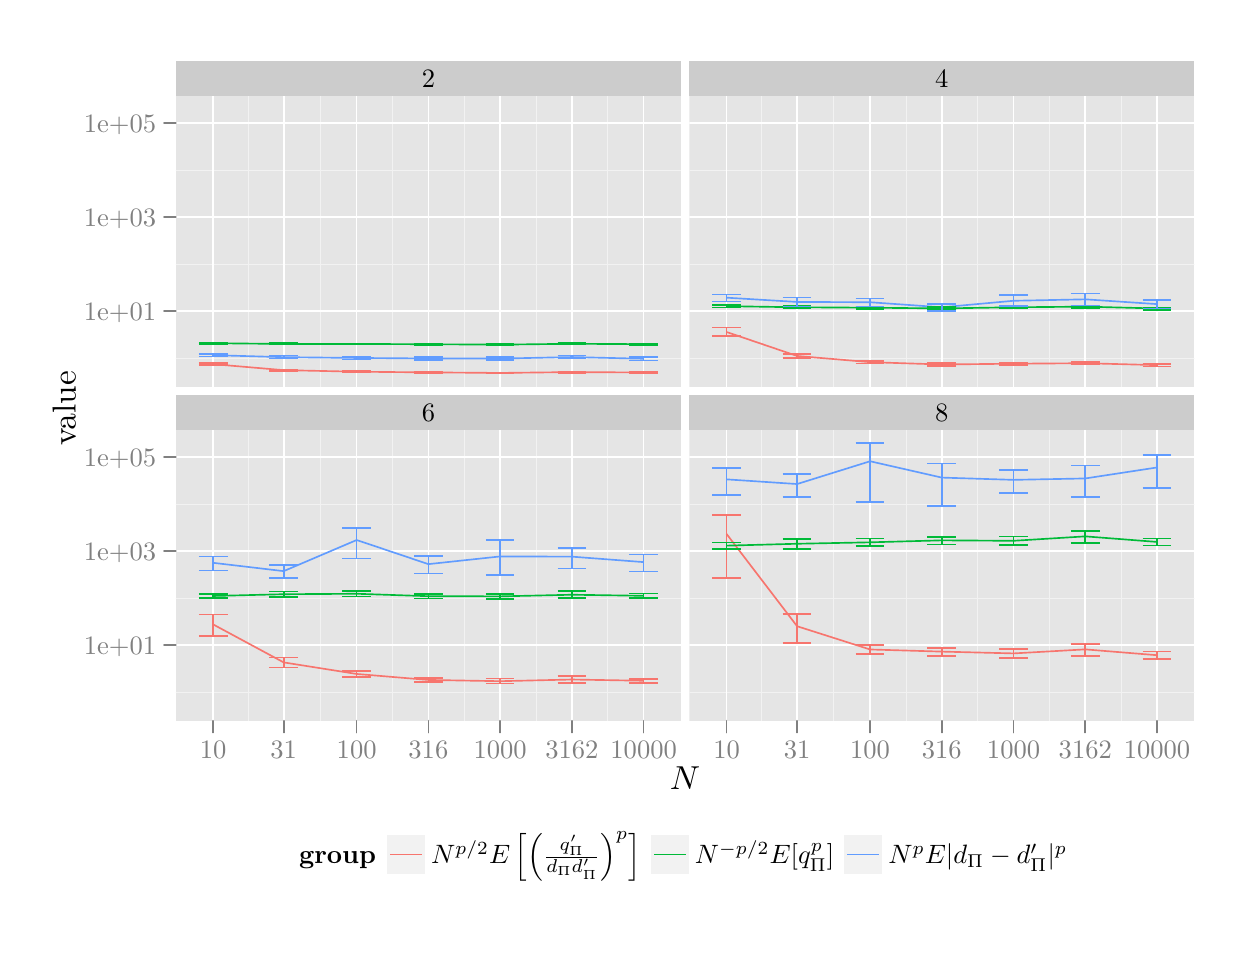
\begin{tikzpicture}[x=1pt,y=1pt]
\definecolor[named]{drawColor}{rgb}{0.00,0.00,0.00}
\definecolor[named]{fillColor}{rgb}{1.00,1.00,1.00}
\fill[color=fillColor,fill opacity=0.00,] (0,0) rectangle (433.62,325.21);
\begin{scope}
\path[clip] (  0.00,  0.00) rectangle (433.62,325.21);
\definecolor[named]{drawColor}{rgb}{0.41,0.16,0.58}
\end{scope}
\begin{scope}
\path[clip] (  0.00,  0.00) rectangle (433.62,325.21);
\definecolor[named]{drawColor}{rgb}{0.41,0.16,0.58}
\end{scope}
\begin{scope}
\path[clip] (  0.00,  0.00) rectangle (433.62,325.21);
\definecolor[named]{drawColor}{rgb}{0.41,0.16,0.58}
\end{scope}
\begin{scope}
\path[clip] (  0.00,  0.00) rectangle (433.62,325.21);
\definecolor[named]{drawColor}{rgb}{0.41,0.16,0.58}
\end{scope}
\begin{scope}
\path[clip] (  0.00,  0.00) rectangle (433.62,325.21);
\definecolor[named]{drawColor}{rgb}{0.41,0.16,0.58}
\end{scope}
\begin{scope}
\path[clip] (  0.00,  0.00) rectangle (433.62,325.21);
\definecolor[named]{drawColor}{rgb}{0.41,0.16,0.58}
\end{scope}
\begin{scope}
\path[clip] (  0.00,  0.00) rectangle (433.62,325.21);
\definecolor[named]{drawColor}{rgb}{0.41,0.16,0.58}
\end{scope}
\begin{scope}
\path[clip] (  0.00,  0.00) rectangle (433.62,325.21);
\definecolor[named]{drawColor}{rgb}{0.41,0.16,0.58}
\end{scope}
\begin{scope}
\path[clip] ( 53.55,195.47) rectangle (236.06,300.54);
\definecolor[named]{drawColor}{rgb}{0.41,0.16,0.58}
\end{scope}
\begin{scope}
\path[clip] (  0.00,  0.00) rectangle (433.62,325.21);
\definecolor[named]{drawColor}{rgb}{0.41,0.16,0.58}
\end{scope}
\begin{scope}
\path[clip] (239.07,195.47) rectangle (421.58,300.54);
\definecolor[named]{drawColor}{rgb}{0.41,0.16,0.58}
\end{scope}
\begin{scope}
\path[clip] (  0.00,  0.00) rectangle (433.62,325.21);
\definecolor[named]{drawColor}{rgb}{0.41,0.16,0.58}
\end{scope}
\begin{scope}
\path[clip] ( 53.55, 74.76) rectangle (236.06,179.83);
\definecolor[named]{drawColor}{rgb}{0.41,0.16,0.58}
\end{scope}
\begin{scope}
\path[clip] (  0.00,  0.00) rectangle (433.62,325.21);
\definecolor[named]{drawColor}{rgb}{0.41,0.16,0.58}
\end{scope}
\begin{scope}
\path[clip] (239.07, 74.76) rectangle (421.58,179.83);
\definecolor[named]{drawColor}{rgb}{0.41,0.16,0.58}
\end{scope}
\begin{scope}
\path[clip] (  0.00,  0.00) rectangle (433.62,325.21);
\definecolor[named]{drawColor}{rgb}{0.41,0.16,0.58}
\end{scope}
\begin{scope}
\path[clip] (  0.00,  0.00) rectangle (433.62,325.21);
\definecolor[named]{drawColor}{rgb}{0.41,0.16,0.58}
\end{scope}
\begin{scope}
\path[clip] (  0.00,  0.00) rectangle (433.62,325.21);
\definecolor[named]{drawColor}{rgb}{0.41,0.16,0.58}
\end{scope}
\begin{scope}
\path[clip] (  0.00,  0.00) rectangle (433.62,325.21);
\definecolor[named]{drawColor}{rgb}{0.41,0.16,0.58}
\end{scope}
\begin{scope}
\path[clip] (  0.00,  0.00) rectangle (433.62,325.21);
\definecolor[named]{drawColor}{rgb}{0.41,0.16,0.58}
\end{scope}
\begin{scope}
\path[clip] (  0.00,  0.00) rectangle (433.62,325.21);
\definecolor[named]{drawColor}{rgb}{0.41,0.16,0.58}
\end{scope}
\begin{scope}
\path[clip] (  0.00,  0.00) rectangle (433.62,325.21);
\definecolor[named]{drawColor}{rgb}{0.41,0.16,0.58}
\end{scope}
\begin{scope}
\path[clip] (  0.00,  0.00) rectangle (433.62,325.21);
\definecolor[named]{drawColor}{rgb}{0.41,0.16,0.58}
\end{scope}
\begin{scope}
\path[clip] (  0.00,  0.00) rectangle (433.62,325.21);
\definecolor[named]{drawColor}{rgb}{0.41,0.16,0.58}
\end{scope}
\begin{scope}
\path[clip] (  0.00,  0.00) rectangle (433.62,325.21);
\definecolor[named]{drawColor}{rgb}{0.41,0.16,0.58}
\end{scope}
\begin{scope}
\path[clip] (  0.00,  0.00) rectangle (433.62,325.21);
\definecolor[named]{drawColor}{rgb}{0.41,0.16,0.58}
\end{scope}
\begin{scope}
\path[clip] (  0.00,  0.00) rectangle (433.62,325.21);
\definecolor[named]{drawColor}{rgb}{0.41,0.16,0.58}
\end{scope}
\begin{scope}
\path[clip] (  0.00,  0.00) rectangle (433.62,325.21);
\definecolor[named]{drawColor}{rgb}{0.41,0.16,0.58}
\end{scope}
\begin{scope}
\path[clip] (  0.00,  0.00) rectangle (433.62,325.21);
\definecolor[named]{drawColor}{rgb}{0.41,0.16,0.58}
\end{scope}
\begin{scope}
\path[clip] (  0.00,  0.00) rectangle (433.62,325.21);
\definecolor[named]{drawColor}{rgb}{0.41,0.16,0.58}
\end{scope}
\begin{scope}
\path[clip] (  0.00,  0.00) rectangle (433.62,325.21);
\definecolor[named]{drawColor}{rgb}{0.41,0.16,0.58}
\end{scope}
\begin{scope}
\path[clip] (  0.00,  0.00) rectangle (433.62,325.21);
\definecolor[named]{drawColor}{rgb}{0.41,0.16,0.58}
\end{scope}
\begin{scope}
\path[clip] (  0.00,  0.00) rectangle (433.62,325.21);
\definecolor[named]{drawColor}{rgb}{0.41,0.16,0.58}
\end{scope}
\begin{scope}
\path[clip] (  0.00,  0.00) rectangle (433.62,325.21);
\definecolor[named]{drawColor}{rgb}{0.41,0.16,0.58}
\end{scope}
\begin{scope}
\path[clip] (  0.00,  0.00) rectangle (433.62,325.21);
\definecolor[named]{drawColor}{rgb}{0.41,0.16,0.58}
\end{scope}
\begin{scope}
\path[clip] (  0.00,  0.00) rectangle (433.62,325.21);
\definecolor[named]{drawColor}{rgb}{0.41,0.16,0.58}
\end{scope}
\begin{scope}
\path[clip] (  0.00,  0.00) rectangle (433.62,325.21);
\definecolor[named]{drawColor}{rgb}{0.41,0.16,0.58}
\end{scope}
\begin{scope}
\path[clip] (  0.00,  0.00) rectangle (433.62,325.21);
\definecolor[named]{drawColor}{rgb}{0.41,0.16,0.58}
\end{scope}
\begin{scope}
\path[clip] (  0.00,  0.00) rectangle (433.62,325.21);
\definecolor[named]{drawColor}{rgb}{0.41,0.16,0.58}
\end{scope}
\begin{scope}
\path[clip] (  0.00,  0.00) rectangle (433.62,325.21);
\definecolor[named]{drawColor}{rgb}{0.41,0.16,0.58}
\end{scope}
\begin{scope}
\path[clip] (  0.00,  0.00) rectangle (433.62,325.21);
\definecolor[named]{drawColor}{rgb}{0.41,0.16,0.58}
\end{scope}
\begin{scope}
\path[clip] (  0.00,  0.00) rectangle (433.62,325.21);
\definecolor[named]{drawColor}{rgb}{0.41,0.16,0.58}
\end{scope}
\begin{scope}
\path[clip] (  0.00,  0.00) rectangle (433.62,325.21);
\definecolor[named]{drawColor}{rgb}{0.41,0.16,0.58}
\end{scope}
\begin{scope}
\path[clip] (  0.00,  0.00) rectangle (433.62,325.21);
\definecolor[named]{drawColor}{rgb}{0.41,0.16,0.58}
\end{scope}
\begin{scope}
\path[clip] (  0.00,  0.00) rectangle (433.62,325.21);
\definecolor[named]{drawColor}{rgb}{0.41,0.16,0.58}
\end{scope}
\begin{scope}
\path[clip] (  0.00,  0.00) rectangle (433.62,325.21);
\definecolor[named]{drawColor}{rgb}{0.41,0.16,0.58}
\end{scope}
\begin{scope}
\path[clip] (  0.00,  0.00) rectangle (433.62,325.21);
\definecolor[named]{drawColor}{rgb}{0.41,0.16,0.58}
\end{scope}
\begin{scope}
\path[clip] (  0.00,  0.00) rectangle (433.62,325.21);
\definecolor[named]{drawColor}{rgb}{0.41,0.16,0.58}
\end{scope}
\begin{scope}
\path[clip] (  0.00,  0.00) rectangle (433.62,325.21);
\definecolor[named]{drawColor}{rgb}{0.41,0.16,0.58}
\definecolor[named]{fillColor}{rgb}{1.00,1.00,1.00}

\draw[fill=fillColor,draw opacity=0.00,] (  0.00,  0.00) rectangle (433.62,325.21);
\end{scope}
\begin{scope}
\path[clip] (  0.00,  0.00) rectangle (433.62,325.21);
\definecolor[named]{drawColor}{rgb}{0.41,0.16,0.58}
\end{scope}
\begin{scope}
\path[clip] ( 53.55,195.47) rectangle (236.06,300.54);
\definecolor[named]{drawColor}{rgb}{0.41,0.16,0.58}
\definecolor[named]{fillColor}{rgb}{0.90,0.90,0.90}

\draw[fill=fillColor,draw opacity=0.00,] ( 53.55,195.47) rectangle (236.06,300.54);
\definecolor[named]{drawColor}{rgb}{0.95,0.95,0.95}

\draw[color=drawColor,line width= 0.3pt,line cap=round,line join=round,fill opacity=0.00,] ( 53.55,205.77) --
	(236.06,205.77);

\draw[color=drawColor,line width= 0.3pt,line cap=round,line join=round,fill opacity=0.00,] ( 53.55,239.78) --
	(236.06,239.78);

\draw[color=drawColor,line width= 0.3pt,line cap=round,line join=round,fill opacity=0.00,] ( 53.55,273.79) --
	(236.06,273.79);

\draw[color=drawColor,line width= 0.3pt,line cap=round,line join=round,fill opacity=0.00,] ( 79.77,195.47) --
	( 79.77,300.54);

\draw[color=drawColor,line width= 0.3pt,line cap=round,line join=round,fill opacity=0.00,] (105.69,195.47) --
	(105.69,300.54);

\draw[color=drawColor,line width= 0.3pt,line cap=round,line join=round,fill opacity=0.00,] (131.83,195.47) --
	(131.83,300.54);

\draw[color=drawColor,line width= 0.3pt,line cap=round,line join=round,fill opacity=0.00,] (157.76,195.47) --
	(157.76,300.54);

\draw[color=drawColor,line width= 0.3pt,line cap=round,line join=round,fill opacity=0.00,] (183.69,195.47) --
	(183.69,300.54);

\draw[color=drawColor,line width= 0.3pt,line cap=round,line join=round,fill opacity=0.00,] (209.61,195.47) --
	(209.61,300.54);
\definecolor[named]{drawColor}{rgb}{1.00,1.00,1.00}

\draw[color=drawColor,line width= 0.6pt,line cap=round,line join=round,fill opacity=0.00,] ( 53.55,222.77) --
	(236.06,222.77);

\draw[color=drawColor,line width= 0.6pt,line cap=round,line join=round,fill opacity=0.00,] ( 53.55,256.78) --
	(236.06,256.78);

\draw[color=drawColor,line width= 0.6pt,line cap=round,line join=round,fill opacity=0.00,] ( 53.55,290.80) --
	(236.06,290.80);

\draw[color=drawColor,line width= 0.6pt,line cap=round,line join=round,fill opacity=0.00,] ( 67.03,195.47) --
	( 67.03,300.54);

\draw[color=drawColor,line width= 0.6pt,line cap=round,line join=round,fill opacity=0.00,] ( 92.51,195.47) --
	( 92.51,300.54);

\draw[color=drawColor,line width= 0.6pt,line cap=round,line join=round,fill opacity=0.00,] (118.88,195.47) --
	(118.88,300.54);

\draw[color=drawColor,line width= 0.6pt,line cap=round,line join=round,fill opacity=0.00,] (144.79,195.47) --
	(144.79,300.54);

\draw[color=drawColor,line width= 0.6pt,line cap=round,line join=round,fill opacity=0.00,] (170.73,195.47) --
	(170.73,300.54);

\draw[color=drawColor,line width= 0.6pt,line cap=round,line join=round,fill opacity=0.00,] (196.65,195.47) --
	(196.65,300.54);

\draw[color=drawColor,line width= 0.6pt,line cap=round,line join=round,fill opacity=0.00,] (222.58,195.47) --
	(222.58,300.54);
\definecolor[named]{drawColor}{rgb}{0.97,0.46,0.43}

\draw[color=drawColor,line width= 0.6pt,line join=round,fill opacity=0.00,] ( 67.03,203.62) --
	( 92.51,201.45) --
	(118.88,200.89) --
	(144.79,200.64) --
	(170.73,200.45) --
	(196.65,200.75) --
	(222.58,200.61);
\definecolor[named]{drawColor}{rgb}{0.00,0.73,0.22}

\draw[color=drawColor,line width= 0.6pt,line join=round,fill opacity=0.00,] ( 67.03,211.18) --
	( 92.51,210.93) --
	(118.88,210.93) --
	(144.79,210.81) --
	(170.73,210.67) --
	(196.65,210.98) --
	(222.58,210.84);
\definecolor[named]{drawColor}{rgb}{0.38,0.61,1.00}

\draw[color=drawColor,line width= 0.6pt,line join=round,fill opacity=0.00,] ( 67.03,206.87) --
	( 92.51,206.15) --
	(118.88,205.86) --
	(144.79,205.67) --
	(170.73,205.63) --
	(196.65,206.19) --
	(222.58,205.57);
\definecolor[named]{drawColor}{rgb}{0.97,0.46,0.43}

\draw[color=drawColor,line width= 0.6pt,line join=round,fill opacity=0.00,] ( 61.85,203.97) --
	( 72.22,203.97);

\draw[color=drawColor,line width= 0.6pt,line join=round,fill opacity=0.00,] ( 67.03,203.97) --
	( 67.03,203.29);

\draw[color=drawColor,line width= 0.6pt,line join=round,fill opacity=0.00,] ( 61.85,203.29) --
	( 72.22,203.29);

\draw[color=drawColor,line width= 0.6pt,line join=round,fill opacity=0.00,] ( 87.32,201.67) --
	( 97.69,201.67);

\draw[color=drawColor,line width= 0.6pt,line join=round,fill opacity=0.00,] ( 92.51,201.67) --
	( 92.51,201.22);

\draw[color=drawColor,line width= 0.6pt,line join=round,fill opacity=0.00,] ( 87.32,201.22) --
	( 97.69,201.22);

\draw[color=drawColor,line width= 0.6pt,line join=round,fill opacity=0.00,] (113.69,201.09) --
	(124.06,201.09);

\draw[color=drawColor,line width= 0.6pt,line join=round,fill opacity=0.00,] (118.88,201.09) --
	(118.88,200.69);

\draw[color=drawColor,line width= 0.6pt,line join=round,fill opacity=0.00,] (113.69,200.69) --
	(124.06,200.69);

\draw[color=drawColor,line width= 0.6pt,line join=round,fill opacity=0.00,] (139.60,200.84) --
	(149.97,200.84);

\draw[color=drawColor,line width= 0.6pt,line join=round,fill opacity=0.00,] (144.79,200.84) --
	(144.79,200.43);

\draw[color=drawColor,line width= 0.6pt,line join=round,fill opacity=0.00,] (139.60,200.43) --
	(149.97,200.43);

\draw[color=drawColor,line width= 0.6pt,line join=round,fill opacity=0.00,] (165.54,200.66) --
	(175.91,200.66);

\draw[color=drawColor,line width= 0.6pt,line join=round,fill opacity=0.00,] (170.73,200.66) --
	(170.73,200.25);

\draw[color=drawColor,line width= 0.6pt,line join=round,fill opacity=0.00,] (165.54,200.25) --
	(175.91,200.25);

\draw[color=drawColor,line width= 0.6pt,line join=round,fill opacity=0.00,] (191.47,200.94) --
	(201.83,200.94);

\draw[color=drawColor,line width= 0.6pt,line join=round,fill opacity=0.00,] (196.65,200.94) --
	(196.65,200.54);

\draw[color=drawColor,line width= 0.6pt,line join=round,fill opacity=0.00,] (191.47,200.54) --
	(201.83,200.54);

\draw[color=drawColor,line width= 0.6pt,line join=round,fill opacity=0.00,] (217.39,200.82) --
	(227.76,200.82);

\draw[color=drawColor,line width= 0.6pt,line join=round,fill opacity=0.00,] (222.58,200.82) --
	(222.58,200.41);

\draw[color=drawColor,line width= 0.6pt,line join=round,fill opacity=0.00,] (217.39,200.41) --
	(227.76,200.41);
\definecolor[named]{drawColor}{rgb}{0.00,0.73,0.22}

\draw[color=drawColor,line width= 0.6pt,line join=round,fill opacity=0.00,] ( 61.85,211.38) --
	( 72.22,211.38);

\draw[color=drawColor,line width= 0.6pt,line join=round,fill opacity=0.00,] ( 67.03,211.38) --
	( 67.03,210.97);

\draw[color=drawColor,line width= 0.6pt,line join=round,fill opacity=0.00,] ( 61.85,210.97) --
	( 72.22,210.97);

\draw[color=drawColor,line width= 0.6pt,line join=round,fill opacity=0.00,] ( 87.32,211.15) --
	( 97.69,211.15);

\draw[color=drawColor,line width= 0.6pt,line join=round,fill opacity=0.00,] ( 92.51,211.15) --
	( 92.51,210.73);

\draw[color=drawColor,line width= 0.6pt,line join=round,fill opacity=0.00,] ( 87.32,210.73) --
	( 97.69,210.73);

\draw[color=drawColor,line width= 0.6pt,line join=round,fill opacity=0.00,] (113.69,211.12) --
	(124.06,211.12);

\draw[color=drawColor,line width= 0.6pt,line join=round,fill opacity=0.00,] (118.88,211.12) --
	(118.88,210.73);

\draw[color=drawColor,line width= 0.6pt,line join=round,fill opacity=0.00,] (113.69,210.73) --
	(124.06,210.73);

\draw[color=drawColor,line width= 0.6pt,line join=round,fill opacity=0.00,] (139.60,210.99) --
	(149.97,210.99);

\draw[color=drawColor,line width= 0.6pt,line join=round,fill opacity=0.00,] (144.79,210.99) --
	(144.79,210.60);

\draw[color=drawColor,line width= 0.6pt,line join=round,fill opacity=0.00,] (139.60,210.60) --
	(149.97,210.60);

\draw[color=drawColor,line width= 0.6pt,line join=round,fill opacity=0.00,] (165.54,210.86) --
	(175.91,210.86);

\draw[color=drawColor,line width= 0.6pt,line join=round,fill opacity=0.00,] (170.73,210.86) --
	(170.73,210.48);

\draw[color=drawColor,line width= 0.6pt,line join=round,fill opacity=0.00,] (165.54,210.48) --
	(175.91,210.48);

\draw[color=drawColor,line width= 0.6pt,line join=round,fill opacity=0.00,] (191.47,211.18) --
	(201.83,211.18);

\draw[color=drawColor,line width= 0.6pt,line join=round,fill opacity=0.00,] (196.65,211.18) --
	(196.65,210.77);

\draw[color=drawColor,line width= 0.6pt,line join=round,fill opacity=0.00,] (191.47,210.77) --
	(201.83,210.77);

\draw[color=drawColor,line width= 0.6pt,line join=round,fill opacity=0.00,] (217.39,211.05) --
	(227.76,211.05);

\draw[color=drawColor,line width= 0.6pt,line join=round,fill opacity=0.00,] (222.58,211.05) --
	(222.58,210.63);

\draw[color=drawColor,line width= 0.6pt,line join=round,fill opacity=0.00,] (217.39,210.63) --
	(227.76,210.63);
\definecolor[named]{drawColor}{rgb}{0.38,0.61,1.00}

\draw[color=drawColor,line width= 0.6pt,line join=round,fill opacity=0.00,] ( 61.85,207.36) --
	( 72.22,207.36);

\draw[color=drawColor,line width= 0.6pt,line join=round,fill opacity=0.00,] ( 67.03,207.36) --
	( 67.03,206.33);

\draw[color=drawColor,line width= 0.6pt,line join=round,fill opacity=0.00,] ( 61.85,206.33) --
	( 72.22,206.33);

\draw[color=drawColor,line width= 0.6pt,line join=round,fill opacity=0.00,] ( 87.32,206.72) --
	( 97.69,206.72);

\draw[color=drawColor,line width= 0.6pt,line join=round,fill opacity=0.00,] ( 92.51,206.72) --
	( 92.51,205.63);

\draw[color=drawColor,line width= 0.6pt,line join=round,fill opacity=0.00,] ( 87.32,205.63) --
	( 97.69,205.63);

\draw[color=drawColor,line width= 0.6pt,line join=round,fill opacity=0.00,] (113.69,206.40) --
	(124.06,206.40);

\draw[color=drawColor,line width= 0.6pt,line join=round,fill opacity=0.00,] (118.88,206.40) --
	(118.88,205.30);

\draw[color=drawColor,line width= 0.6pt,line join=round,fill opacity=0.00,] (113.69,205.30) --
	(124.06,205.30);

\draw[color=drawColor,line width= 0.6pt,line join=round,fill opacity=0.00,] (139.60,206.17) --
	(149.97,206.17);

\draw[color=drawColor,line width= 0.6pt,line join=round,fill opacity=0.00,] (144.79,206.17) --
	(144.79,205.15);

\draw[color=drawColor,line width= 0.6pt,line join=round,fill opacity=0.00,] (139.60,205.15) --
	(149.97,205.15);

\draw[color=drawColor,line width= 0.6pt,line join=round,fill opacity=0.00,] (165.54,206.23) --
	(175.91,206.23);

\draw[color=drawColor,line width= 0.6pt,line join=round,fill opacity=0.00,] (170.73,206.23) --
	(170.73,205.01);

\draw[color=drawColor,line width= 0.6pt,line join=round,fill opacity=0.00,] (165.54,205.01) --
	(175.91,205.01);

\draw[color=drawColor,line width= 0.6pt,line join=round,fill opacity=0.00,] (191.47,206.74) --
	(201.83,206.74);

\draw[color=drawColor,line width= 0.6pt,line join=round,fill opacity=0.00,] (196.65,206.74) --
	(196.65,205.64);

\draw[color=drawColor,line width= 0.6pt,line join=round,fill opacity=0.00,] (191.47,205.64) --
	(201.83,205.64);

\draw[color=drawColor,line width= 0.6pt,line join=round,fill opacity=0.00,] (217.39,206.21) --
	(227.76,206.21);

\draw[color=drawColor,line width= 0.6pt,line join=round,fill opacity=0.00,] (222.58,206.21) --
	(222.58,204.91);

\draw[color=drawColor,line width= 0.6pt,line join=round,fill opacity=0.00,] (217.39,204.91) --
	(227.76,204.91);
\end{scope}
\begin{scope}
\path[clip] (  0.00,  0.00) rectangle (433.62,325.21);
\definecolor[named]{drawColor}{rgb}{0.41,0.16,0.58}
\end{scope}
\begin{scope}
\path[clip] (239.07,195.47) rectangle (421.58,300.54);
\definecolor[named]{drawColor}{rgb}{0.41,0.16,0.58}
\definecolor[named]{fillColor}{rgb}{0.90,0.90,0.90}

\draw[fill=fillColor,draw opacity=0.00,] (239.07,195.47) rectangle (421.57,300.54);
\definecolor[named]{drawColor}{rgb}{0.95,0.95,0.95}

\draw[color=drawColor,line width= 0.3pt,line cap=round,line join=round,fill opacity=0.00,] (239.07,205.77) --
	(421.58,205.77);

\draw[color=drawColor,line width= 0.3pt,line cap=round,line join=round,fill opacity=0.00,] (239.07,239.78) --
	(421.58,239.78);

\draw[color=drawColor,line width= 0.3pt,line cap=round,line join=round,fill opacity=0.00,] (239.07,273.79) --
	(421.58,273.79);

\draw[color=drawColor,line width= 0.3pt,line cap=round,line join=round,fill opacity=0.00,] (265.29,195.47) --
	(265.29,300.54);

\draw[color=drawColor,line width= 0.3pt,line cap=round,line join=round,fill opacity=0.00,] (291.21,195.47) --
	(291.21,300.54);

\draw[color=drawColor,line width= 0.3pt,line cap=round,line join=round,fill opacity=0.00,] (317.35,195.47) --
	(317.35,300.54);

\draw[color=drawColor,line width= 0.3pt,line cap=round,line join=round,fill opacity=0.00,] (343.28,195.47) --
	(343.28,300.54);

\draw[color=drawColor,line width= 0.3pt,line cap=round,line join=round,fill opacity=0.00,] (369.21,195.47) --
	(369.21,300.54);

\draw[color=drawColor,line width= 0.3pt,line cap=round,line join=round,fill opacity=0.00,] (395.13,195.47) --
	(395.13,300.54);
\definecolor[named]{drawColor}{rgb}{1.00,1.00,1.00}

\draw[color=drawColor,line width= 0.6pt,line cap=round,line join=round,fill opacity=0.00,] (239.07,222.77) --
	(421.58,222.77);

\draw[color=drawColor,line width= 0.6pt,line cap=round,line join=round,fill opacity=0.00,] (239.07,256.78) --
	(421.58,256.78);

\draw[color=drawColor,line width= 0.6pt,line cap=round,line join=round,fill opacity=0.00,] (239.07,290.80) --
	(421.58,290.80);

\draw[color=drawColor,line width= 0.6pt,line cap=round,line join=round,fill opacity=0.00,] (252.55,195.47) --
	(252.55,300.54);

\draw[color=drawColor,line width= 0.6pt,line cap=round,line join=round,fill opacity=0.00,] (278.03,195.47) --
	(278.03,300.54);

\draw[color=drawColor,line width= 0.6pt,line cap=round,line join=round,fill opacity=0.00,] (304.40,195.47) --
	(304.40,300.54);

\draw[color=drawColor,line width= 0.6pt,line cap=round,line join=round,fill opacity=0.00,] (330.31,195.47) --
	(330.31,300.54);

\draw[color=drawColor,line width= 0.6pt,line cap=round,line join=round,fill opacity=0.00,] (356.25,195.47) --
	(356.25,300.54);

\draw[color=drawColor,line width= 0.6pt,line cap=round,line join=round,fill opacity=0.00,] (382.17,195.47) --
	(382.17,300.54);

\draw[color=drawColor,line width= 0.6pt,line cap=round,line join=round,fill opacity=0.00,] (408.09,195.47) --
	(408.09,300.54);
\definecolor[named]{drawColor}{rgb}{0.97,0.46,0.43}

\draw[color=drawColor,line width= 0.6pt,line join=round,fill opacity=0.00,] (252.55,215.24) --
	(278.03,206.58) --
	(304.40,204.34) --
	(330.31,203.50) --
	(356.25,203.78) --
	(382.17,203.96) --
	(408.09,203.27);
\definecolor[named]{drawColor}{rgb}{0.00,0.73,0.22}

\draw[color=drawColor,line width= 0.6pt,line join=round,fill opacity=0.00,] (252.55,224.58) --
	(278.03,224.17) --
	(304.40,224.02) --
	(330.31,223.76) --
	(356.25,224.17) --
	(382.17,224.40) --
	(408.09,223.74);
\definecolor[named]{drawColor}{rgb}{0.38,0.61,1.00}

\draw[color=drawColor,line width= 0.6pt,line join=round,fill opacity=0.00,] (252.55,227.64) --
	(278.03,226.10) --
	(304.40,225.99) --
	(330.31,224.17) --
	(356.25,226.52) --
	(382.17,227.04) --
	(408.09,225.32);
\definecolor[named]{drawColor}{rgb}{0.97,0.46,0.43}

\draw[color=drawColor,line width= 0.6pt,line join=round,fill opacity=0.00,] (247.36,216.84) --
	(257.73,216.84);

\draw[color=drawColor,line width= 0.6pt,line join=round,fill opacity=0.00,] (252.55,216.84) --
	(252.55,213.69);

\draw[color=drawColor,line width= 0.6pt,line join=round,fill opacity=0.00,] (247.36,213.69) --
	(257.73,213.69);

\draw[color=drawColor,line width= 0.6pt,line join=round,fill opacity=0.00,] (272.84,207.32) --
	(283.21,207.32);

\draw[color=drawColor,line width= 0.6pt,line join=round,fill opacity=0.00,] (278.03,207.32) --
	(278.03,205.85);

\draw[color=drawColor,line width= 0.6pt,line join=round,fill opacity=0.00,] (272.84,205.85) --
	(283.21,205.85);

\draw[color=drawColor,line width= 0.6pt,line join=round,fill opacity=0.00,] (299.21,204.83) --
	(309.58,204.83);

\draw[color=drawColor,line width= 0.6pt,line join=round,fill opacity=0.00,] (304.40,204.83) --
	(304.40,203.84);

\draw[color=drawColor,line width= 0.6pt,line join=round,fill opacity=0.00,] (299.21,203.84) --
	(309.58,203.84);

\draw[color=drawColor,line width= 0.6pt,line join=round,fill opacity=0.00,] (325.12,204.01) --
	(335.49,204.01);

\draw[color=drawColor,line width= 0.6pt,line join=round,fill opacity=0.00,] (330.31,204.01) --
	(330.31,202.98);

\draw[color=drawColor,line width= 0.6pt,line join=round,fill opacity=0.00,] (325.12,202.98) --
	(335.49,202.98);

\draw[color=drawColor,line width= 0.6pt,line join=round,fill opacity=0.00,] (351.06,204.24) --
	(361.43,204.24);

\draw[color=drawColor,line width= 0.6pt,line join=round,fill opacity=0.00,] (356.25,204.24) --
	(356.25,203.27);

\draw[color=drawColor,line width= 0.6pt,line join=round,fill opacity=0.00,] (351.06,203.27) --
	(361.43,203.27);

\draw[color=drawColor,line width= 0.6pt,line join=round,fill opacity=0.00,] (376.98,204.43) --
	(387.35,204.43);

\draw[color=drawColor,line width= 0.6pt,line join=round,fill opacity=0.00,] (382.17,204.43) --
	(382.17,203.49);

\draw[color=drawColor,line width= 0.6pt,line join=round,fill opacity=0.00,] (376.98,203.49) --
	(387.35,203.49);

\draw[color=drawColor,line width= 0.6pt,line join=round,fill opacity=0.00,] (402.91,203.72) --
	(413.28,203.72);

\draw[color=drawColor,line width= 0.6pt,line join=round,fill opacity=0.00,] (408.09,203.72) --
	(408.09,202.82);

\draw[color=drawColor,line width= 0.6pt,line join=round,fill opacity=0.00,] (402.91,202.82) --
	(413.28,202.82);
\definecolor[named]{drawColor}{rgb}{0.00,0.73,0.22}

\draw[color=drawColor,line width= 0.6pt,line join=round,fill opacity=0.00,] (247.36,224.99) --
	(257.73,224.99);

\draw[color=drawColor,line width= 0.6pt,line join=round,fill opacity=0.00,] (252.55,224.99) --
	(252.55,224.14);

\draw[color=drawColor,line width= 0.6pt,line join=round,fill opacity=0.00,] (247.36,224.14) --
	(257.73,224.14);

\draw[color=drawColor,line width= 0.6pt,line join=round,fill opacity=0.00,] (272.84,224.65) --
	(283.21,224.65);

\draw[color=drawColor,line width= 0.6pt,line join=round,fill opacity=0.00,] (278.03,224.65) --
	(278.03,223.69);

\draw[color=drawColor,line width= 0.6pt,line join=round,fill opacity=0.00,] (272.84,223.69) --
	(283.21,223.69);

\draw[color=drawColor,line width= 0.6pt,line join=round,fill opacity=0.00,] (299.21,224.44) --
	(309.58,224.44);

\draw[color=drawColor,line width= 0.6pt,line join=round,fill opacity=0.00,] (304.40,224.44) --
	(304.40,223.57);

\draw[color=drawColor,line width= 0.6pt,line join=round,fill opacity=0.00,] (299.21,223.57) --
	(309.58,223.57);

\draw[color=drawColor,line width= 0.6pt,line join=round,fill opacity=0.00,] (325.12,224.26) --
	(335.49,224.26);

\draw[color=drawColor,line width= 0.6pt,line join=round,fill opacity=0.00,] (330.31,224.26) --
	(330.31,223.28);

\draw[color=drawColor,line width= 0.6pt,line join=round,fill opacity=0.00,] (325.12,223.28) --
	(335.49,223.28);

\draw[color=drawColor,line width= 0.6pt,line join=round,fill opacity=0.00,] (351.06,224.62) --
	(361.43,224.62);

\draw[color=drawColor,line width= 0.6pt,line join=round,fill opacity=0.00,] (356.25,224.62) --
	(356.25,223.69);

\draw[color=drawColor,line width= 0.6pt,line join=round,fill opacity=0.00,] (351.06,223.69) --
	(361.43,223.69);

\draw[color=drawColor,line width= 0.6pt,line join=round,fill opacity=0.00,] (376.98,224.86) --
	(387.35,224.86);

\draw[color=drawColor,line width= 0.6pt,line join=round,fill opacity=0.00,] (382.17,224.86) --
	(382.17,223.93);

\draw[color=drawColor,line width= 0.6pt,line join=round,fill opacity=0.00,] (376.98,223.93) --
	(387.35,223.93);

\draw[color=drawColor,line width= 0.6pt,line join=round,fill opacity=0.00,] (402.91,224.15) --
	(413.28,224.15);

\draw[color=drawColor,line width= 0.6pt,line join=round,fill opacity=0.00,] (408.09,224.15) --
	(408.09,223.29);

\draw[color=drawColor,line width= 0.6pt,line join=round,fill opacity=0.00,] (402.91,223.29) --
	(413.28,223.29);
\definecolor[named]{drawColor}{rgb}{0.38,0.61,1.00}

\draw[color=drawColor,line width= 0.6pt,line join=round,fill opacity=0.00,] (247.36,228.81) --
	(257.73,228.81);

\draw[color=drawColor,line width= 0.6pt,line join=round,fill opacity=0.00,] (252.55,228.81) --
	(252.55,226.29);

\draw[color=drawColor,line width= 0.6pt,line join=round,fill opacity=0.00,] (247.36,226.29) --
	(257.73,226.29);

\draw[color=drawColor,line width= 0.6pt,line join=round,fill opacity=0.00,] (272.84,227.66) --
	(283.21,227.66);

\draw[color=drawColor,line width= 0.6pt,line join=round,fill opacity=0.00,] (278.03,227.66) --
	(278.03,224.40);

\draw[color=drawColor,line width= 0.6pt,line join=round,fill opacity=0.00,] (272.84,224.40) --
	(283.21,224.40);

\draw[color=drawColor,line width= 0.6pt,line join=round,fill opacity=0.00,] (299.21,227.34) --
	(309.58,227.34);

\draw[color=drawColor,line width= 0.6pt,line join=round,fill opacity=0.00,] (304.40,227.34) --
	(304.40,224.49);

\draw[color=drawColor,line width= 0.6pt,line join=round,fill opacity=0.00,] (299.21,224.49) --
	(309.58,224.49);

\draw[color=drawColor,line width= 0.6pt,line join=round,fill opacity=0.00,] (325.12,225.43) --
	(335.49,225.43);

\draw[color=drawColor,line width= 0.6pt,line join=round,fill opacity=0.00,] (330.31,225.43) --
	(330.31,222.87);

\draw[color=drawColor,line width= 0.6pt,line join=round,fill opacity=0.00,] (325.12,222.87) --
	(335.49,222.87);

\draw[color=drawColor,line width= 0.6pt,line join=round,fill opacity=0.00,] (351.06,228.49) --
	(361.43,228.49);

\draw[color=drawColor,line width= 0.6pt,line join=round,fill opacity=0.00,] (356.25,228.49) --
	(356.25,224.54);

\draw[color=drawColor,line width= 0.6pt,line join=round,fill opacity=0.00,] (351.06,224.54) --
	(361.43,224.54);

\draw[color=drawColor,line width= 0.6pt,line join=round,fill opacity=0.00,] (376.98,229.16) --
	(387.35,229.16);

\draw[color=drawColor,line width= 0.6pt,line join=round,fill opacity=0.00,] (382.17,229.16) --
	(382.17,224.82);

\draw[color=drawColor,line width= 0.6pt,line join=round,fill opacity=0.00,] (376.98,224.82) --
	(387.35,224.82);

\draw[color=drawColor,line width= 0.6pt,line join=round,fill opacity=0.00,] (402.91,226.88) --
	(413.28,226.88);

\draw[color=drawColor,line width= 0.6pt,line join=round,fill opacity=0.00,] (408.09,226.88) --
	(408.09,223.76);

\draw[color=drawColor,line width= 0.6pt,line join=round,fill opacity=0.00,] (402.91,223.76) --
	(413.28,223.76);
\end{scope}
\begin{scope}
\path[clip] (  0.00,  0.00) rectangle (433.62,325.21);
\definecolor[named]{drawColor}{rgb}{0.41,0.16,0.58}
\end{scope}
\begin{scope}
\path[clip] ( 53.55, 74.76) rectangle (236.06,179.83);
\definecolor[named]{drawColor}{rgb}{0.41,0.16,0.58}
\definecolor[named]{fillColor}{rgb}{0.90,0.90,0.90}

\draw[fill=fillColor,draw opacity=0.00,] ( 53.55, 74.76) rectangle (236.06,179.83);
\definecolor[named]{drawColor}{rgb}{0.95,0.95,0.95}

\draw[color=drawColor,line width= 0.3pt,line cap=round,line join=round,fill opacity=0.00,] ( 53.55, 85.06) --
	(236.06, 85.06);

\draw[color=drawColor,line width= 0.3pt,line cap=round,line join=round,fill opacity=0.00,] ( 53.55,119.07) --
	(236.06,119.07);

\draw[color=drawColor,line width= 0.3pt,line cap=round,line join=round,fill opacity=0.00,] ( 53.55,153.08) --
	(236.06,153.08);

\draw[color=drawColor,line width= 0.3pt,line cap=round,line join=round,fill opacity=0.00,] ( 79.77, 74.76) --
	( 79.77,179.83);

\draw[color=drawColor,line width= 0.3pt,line cap=round,line join=round,fill opacity=0.00,] (105.69, 74.76) --
	(105.69,179.83);

\draw[color=drawColor,line width= 0.3pt,line cap=round,line join=round,fill opacity=0.00,] (131.83, 74.76) --
	(131.83,179.83);

\draw[color=drawColor,line width= 0.3pt,line cap=round,line join=round,fill opacity=0.00,] (157.76, 74.76) --
	(157.76,179.83);

\draw[color=drawColor,line width= 0.3pt,line cap=round,line join=round,fill opacity=0.00,] (183.69, 74.76) --
	(183.69,179.83);

\draw[color=drawColor,line width= 0.3pt,line cap=round,line join=round,fill opacity=0.00,] (209.61, 74.76) --
	(209.61,179.83);
\definecolor[named]{drawColor}{rgb}{1.00,1.00,1.00}

\draw[color=drawColor,line width= 0.6pt,line cap=round,line join=round,fill opacity=0.00,] ( 53.55,102.06) --
	(236.06,102.06);

\draw[color=drawColor,line width= 0.6pt,line cap=round,line join=round,fill opacity=0.00,] ( 53.55,136.07) --
	(236.06,136.07);

\draw[color=drawColor,line width= 0.6pt,line cap=round,line join=round,fill opacity=0.00,] ( 53.55,170.09) --
	(236.06,170.09);

\draw[color=drawColor,line width= 0.6pt,line cap=round,line join=round,fill opacity=0.00,] ( 67.03, 74.76) --
	( 67.03,179.83);

\draw[color=drawColor,line width= 0.6pt,line cap=round,line join=round,fill opacity=0.00,] ( 92.51, 74.76) --
	( 92.51,179.83);

\draw[color=drawColor,line width= 0.6pt,line cap=round,line join=round,fill opacity=0.00,] (118.88, 74.76) --
	(118.88,179.83);

\draw[color=drawColor,line width= 0.6pt,line cap=round,line join=round,fill opacity=0.00,] (144.79, 74.76) --
	(144.79,179.83);

\draw[color=drawColor,line width= 0.6pt,line cap=round,line join=round,fill opacity=0.00,] (170.73, 74.76) --
	(170.73,179.83);

\draw[color=drawColor,line width= 0.6pt,line cap=round,line join=round,fill opacity=0.00,] (196.65, 74.76) --
	(196.65,179.83);

\draw[color=drawColor,line width= 0.6pt,line cap=round,line join=round,fill opacity=0.00,] (222.58, 74.76) --
	(222.58,179.83);
\definecolor[named]{drawColor}{rgb}{0.97,0.46,0.43}

\draw[color=drawColor,line width= 0.6pt,line join=round,fill opacity=0.00,] ( 67.03,109.57) --
	( 92.51, 95.85) --
	(118.88, 91.67) --
	(144.79, 89.51) --
	(170.73, 89.06) --
	(196.65, 89.66) --
	(222.58, 89.22);
\definecolor[named]{drawColor}{rgb}{0.00,0.73,0.22}

\draw[color=drawColor,line width= 0.6pt,line join=round,fill opacity=0.00,] ( 67.03,119.85) --
	( 92.51,120.49) --
	(118.88,120.65) --
	(144.79,119.77) --
	(170.73,119.71) --
	(196.65,120.30) --
	(222.58,119.91);
\definecolor[named]{drawColor}{rgb}{0.38,0.61,1.00}

\draw[color=drawColor,line width= 0.6pt,line join=round,fill opacity=0.00,] ( 67.03,131.83) --
	( 92.51,128.83) --
	(118.88,140.07) --
	(144.79,131.36) --
	(170.73,134.14) --
	(196.65,134.06) --
	(222.58,132.09);
\definecolor[named]{drawColor}{rgb}{0.97,0.46,0.43}

\draw[color=drawColor,line width= 0.6pt,line join=round,fill opacity=0.00,] ( 61.85,113.19) --
	( 72.22,113.19);

\draw[color=drawColor,line width= 0.6pt,line join=round,fill opacity=0.00,] ( 67.03,113.19) --
	( 67.03,105.42);

\draw[color=drawColor,line width= 0.6pt,line join=round,fill opacity=0.00,] ( 61.85,105.42) --
	( 72.22,105.42);

\draw[color=drawColor,line width= 0.6pt,line join=round,fill opacity=0.00,] ( 87.32, 97.57) --
	( 97.69, 97.57);

\draw[color=drawColor,line width= 0.6pt,line join=round,fill opacity=0.00,] ( 92.51, 97.57) --
	( 92.51, 94.02);

\draw[color=drawColor,line width= 0.6pt,line join=round,fill opacity=0.00,] ( 87.32, 94.02) --
	( 97.69, 94.02);

\draw[color=drawColor,line width= 0.6pt,line join=round,fill opacity=0.00,] (113.69, 92.72) --
	(124.06, 92.72);

\draw[color=drawColor,line width= 0.6pt,line join=round,fill opacity=0.00,] (118.88, 92.72) --
	(118.88, 90.62);

\draw[color=drawColor,line width= 0.6pt,line join=round,fill opacity=0.00,] (113.69, 90.62) --
	(124.06, 90.62);

\draw[color=drawColor,line width= 0.6pt,line join=round,fill opacity=0.00,] (139.60, 90.31) --
	(149.97, 90.31);

\draw[color=drawColor,line width= 0.6pt,line join=round,fill opacity=0.00,] (144.79, 90.31) --
	(144.79, 88.73);

\draw[color=drawColor,line width= 0.6pt,line join=round,fill opacity=0.00,] (139.60, 88.73) --
	(149.97, 88.73);

\draw[color=drawColor,line width= 0.6pt,line join=round,fill opacity=0.00,] (165.54, 90.07) --
	(175.91, 90.07);

\draw[color=drawColor,line width= 0.6pt,line join=round,fill opacity=0.00,] (170.73, 90.07) --
	(170.73, 88.17);

\draw[color=drawColor,line width= 0.6pt,line join=round,fill opacity=0.00,] (165.54, 88.17) --
	(175.91, 88.17);

\draw[color=drawColor,line width= 0.6pt,line join=round,fill opacity=0.00,] (191.47, 90.96) --
	(201.83, 90.96);

\draw[color=drawColor,line width= 0.6pt,line join=round,fill opacity=0.00,] (196.65, 90.96) --
	(196.65, 88.35);

\draw[color=drawColor,line width= 0.6pt,line join=round,fill opacity=0.00,] (191.47, 88.35) --
	(201.83, 88.35);

\draw[color=drawColor,line width= 0.6pt,line join=round,fill opacity=0.00,] (217.39, 89.96) --
	(227.76, 89.96);

\draw[color=drawColor,line width= 0.6pt,line join=round,fill opacity=0.00,] (222.58, 89.96) --
	(222.58, 88.33);

\draw[color=drawColor,line width= 0.6pt,line join=round,fill opacity=0.00,] (217.39, 88.33) --
	(227.76, 88.33);
\definecolor[named]{drawColor}{rgb}{0.00,0.73,0.22}

\draw[color=drawColor,line width= 0.6pt,line join=round,fill opacity=0.00,] ( 61.85,120.51) --
	( 72.22,120.51);

\draw[color=drawColor,line width= 0.6pt,line join=round,fill opacity=0.00,] ( 67.03,120.51) --
	( 67.03,119.19);

\draw[color=drawColor,line width= 0.6pt,line join=round,fill opacity=0.00,] ( 61.85,119.19) --
	( 72.22,119.19);

\draw[color=drawColor,line width= 0.6pt,line join=round,fill opacity=0.00,] ( 87.32,121.44) --
	( 97.69,121.44);

\draw[color=drawColor,line width= 0.6pt,line join=round,fill opacity=0.00,] ( 92.51,121.44) --
	( 92.51,119.48);

\draw[color=drawColor,line width= 0.6pt,line join=round,fill opacity=0.00,] ( 87.32,119.48) --
	( 97.69,119.48);

\draw[color=drawColor,line width= 0.6pt,line join=round,fill opacity=0.00,] (113.69,121.57) --
	(124.06,121.57);

\draw[color=drawColor,line width= 0.6pt,line join=round,fill opacity=0.00,] (118.88,121.57) --
	(118.88,119.66);

\draw[color=drawColor,line width= 0.6pt,line join=round,fill opacity=0.00,] (113.69,119.66) --
	(124.06,119.66);

\draw[color=drawColor,line width= 0.6pt,line join=round,fill opacity=0.00,] (139.60,120.49) --
	(149.97,120.49);

\draw[color=drawColor,line width= 0.6pt,line join=round,fill opacity=0.00,] (144.79,120.49) --
	(144.79,118.98);

\draw[color=drawColor,line width= 0.6pt,line join=round,fill opacity=0.00,] (139.60,118.98) --
	(149.97,118.98);

\draw[color=drawColor,line width= 0.6pt,line join=round,fill opacity=0.00,] (165.54,120.55) --
	(175.91,120.55);

\draw[color=drawColor,line width= 0.6pt,line join=round,fill opacity=0.00,] (170.73,120.55) --
	(170.73,118.84);

\draw[color=drawColor,line width= 0.6pt,line join=round,fill opacity=0.00,] (165.54,118.84) --
	(175.91,118.84);

\draw[color=drawColor,line width= 0.6pt,line join=round,fill opacity=0.00,] (191.47,121.60) --
	(201.83,121.60);

\draw[color=drawColor,line width= 0.6pt,line join=round,fill opacity=0.00,] (196.65,121.60) --
	(196.65,119.11);

\draw[color=drawColor,line width= 0.6pt,line join=round,fill opacity=0.00,] (191.47,119.11) --
	(201.83,119.11);

\draw[color=drawColor,line width= 0.6pt,line join=round,fill opacity=0.00,] (217.39,120.74) --
	(227.76,120.74);

\draw[color=drawColor,line width= 0.6pt,line join=round,fill opacity=0.00,] (222.58,120.74) --
	(222.58,119.09);

\draw[color=drawColor,line width= 0.6pt,line join=round,fill opacity=0.00,] (217.39,119.09) --
	(227.76,119.09);
\definecolor[named]{drawColor}{rgb}{0.38,0.61,1.00}

\draw[color=drawColor,line width= 0.6pt,line join=round,fill opacity=0.00,] ( 61.85,134.09) --
	( 72.22,134.09);

\draw[color=drawColor,line width= 0.6pt,line join=round,fill opacity=0.00,] ( 67.03,134.09) --
	( 67.03,129.05);

\draw[color=drawColor,line width= 0.6pt,line join=round,fill opacity=0.00,] ( 61.85,129.05) --
	( 72.22,129.05);

\draw[color=drawColor,line width= 0.6pt,line join=round,fill opacity=0.00,] ( 87.32,131.15) --
	( 97.69,131.15);

\draw[color=drawColor,line width= 0.6pt,line join=round,fill opacity=0.00,] ( 92.51,131.15) --
	( 92.51,126.25);

\draw[color=drawColor,line width= 0.6pt,line join=round,fill opacity=0.00,] ( 87.32,126.25) --
	( 97.69,126.25);

\draw[color=drawColor,line width= 0.6pt,line join=round,fill opacity=0.00,] (113.69,144.50) --
	(124.06,144.50);

\draw[color=drawColor,line width= 0.6pt,line join=round,fill opacity=0.00,] (118.88,144.50) --
	(118.88,133.39);

\draw[color=drawColor,line width= 0.6pt,line join=round,fill opacity=0.00,] (113.69,133.39) --
	(124.06,133.39);

\draw[color=drawColor,line width= 0.6pt,line join=round,fill opacity=0.00,] (139.60,134.18) --
	(149.97,134.18);

\draw[color=drawColor,line width= 0.6pt,line join=round,fill opacity=0.00,] (144.79,134.18) --
	(144.79,128.01);

\draw[color=drawColor,line width= 0.6pt,line join=round,fill opacity=0.00,] (139.60,128.01) --
	(149.97,128.01);

\draw[color=drawColor,line width= 0.6pt,line join=round,fill opacity=0.00,] (165.54,140.10) --
	(175.91,140.10);

\draw[color=drawColor,line width= 0.6pt,line join=round,fill opacity=0.00,] (170.73,140.10) --
	(170.73,127.36);

\draw[color=drawColor,line width= 0.6pt,line join=round,fill opacity=0.00,] (165.54,127.36) --
	(175.91,127.36);

\draw[color=drawColor,line width= 0.6pt,line join=round,fill opacity=0.00,] (191.47,137.13) --
	(201.83,137.13);

\draw[color=drawColor,line width= 0.6pt,line join=round,fill opacity=0.00,] (196.65,137.13) --
	(196.65,129.81);

\draw[color=drawColor,line width= 0.6pt,line join=round,fill opacity=0.00,] (191.47,129.81) --
	(201.83,129.81);

\draw[color=drawColor,line width= 0.6pt,line join=round,fill opacity=0.00,] (217.39,134.80) --
	(227.76,134.80);

\draw[color=drawColor,line width= 0.6pt,line join=round,fill opacity=0.00,] (222.58,134.80) --
	(222.58,128.67);

\draw[color=drawColor,line width= 0.6pt,line join=round,fill opacity=0.00,] (217.39,128.67) --
	(227.76,128.67);
\end{scope}
\begin{scope}
\path[clip] (  0.00,  0.00) rectangle (433.62,325.21);
\definecolor[named]{drawColor}{rgb}{0.41,0.16,0.58}
\end{scope}
\begin{scope}
\path[clip] (239.07, 74.76) rectangle (421.58,179.83);
\definecolor[named]{drawColor}{rgb}{0.41,0.16,0.58}
\definecolor[named]{fillColor}{rgb}{0.90,0.90,0.90}

\draw[fill=fillColor,draw opacity=0.00,] (239.07, 74.76) rectangle (421.57,179.83);
\definecolor[named]{drawColor}{rgb}{0.95,0.95,0.95}

\draw[color=drawColor,line width= 0.3pt,line cap=round,line join=round,fill opacity=0.00,] (239.07, 85.06) --
	(421.58, 85.06);

\draw[color=drawColor,line width= 0.3pt,line cap=round,line join=round,fill opacity=0.00,] (239.07,119.07) --
	(421.58,119.07);

\draw[color=drawColor,line width= 0.3pt,line cap=round,line join=round,fill opacity=0.00,] (239.07,153.08) --
	(421.58,153.08);

\draw[color=drawColor,line width= 0.3pt,line cap=round,line join=round,fill opacity=0.00,] (265.29, 74.76) --
	(265.29,179.83);

\draw[color=drawColor,line width= 0.3pt,line cap=round,line join=round,fill opacity=0.00,] (291.21, 74.76) --
	(291.21,179.83);

\draw[color=drawColor,line width= 0.3pt,line cap=round,line join=round,fill opacity=0.00,] (317.35, 74.76) --
	(317.35,179.83);

\draw[color=drawColor,line width= 0.3pt,line cap=round,line join=round,fill opacity=0.00,] (343.28, 74.76) --
	(343.28,179.83);

\draw[color=drawColor,line width= 0.3pt,line cap=round,line join=round,fill opacity=0.00,] (369.21, 74.76) --
	(369.21,179.83);

\draw[color=drawColor,line width= 0.3pt,line cap=round,line join=round,fill opacity=0.00,] (395.13, 74.76) --
	(395.13,179.83);
\definecolor[named]{drawColor}{rgb}{1.00,1.00,1.00}

\draw[color=drawColor,line width= 0.6pt,line cap=round,line join=round,fill opacity=0.00,] (239.07,102.06) --
	(421.58,102.06);

\draw[color=drawColor,line width= 0.6pt,line cap=round,line join=round,fill opacity=0.00,] (239.07,136.07) --
	(421.58,136.07);

\draw[color=drawColor,line width= 0.6pt,line cap=round,line join=round,fill opacity=0.00,] (239.07,170.09) --
	(421.58,170.09);

\draw[color=drawColor,line width= 0.6pt,line cap=round,line join=round,fill opacity=0.00,] (252.55, 74.76) --
	(252.55,179.83);

\draw[color=drawColor,line width= 0.6pt,line cap=round,line join=round,fill opacity=0.00,] (278.03, 74.76) --
	(278.03,179.83);

\draw[color=drawColor,line width= 0.6pt,line cap=round,line join=round,fill opacity=0.00,] (304.40, 74.76) --
	(304.40,179.83);

\draw[color=drawColor,line width= 0.6pt,line cap=round,line join=round,fill opacity=0.00,] (330.31, 74.76) --
	(330.31,179.83);

\draw[color=drawColor,line width= 0.6pt,line cap=round,line join=round,fill opacity=0.00,] (356.25, 74.76) --
	(356.25,179.83);

\draw[color=drawColor,line width= 0.6pt,line cap=round,line join=round,fill opacity=0.00,] (382.17, 74.76) --
	(382.17,179.83);

\draw[color=drawColor,line width= 0.6pt,line cap=round,line join=round,fill opacity=0.00,] (408.09, 74.76) --
	(408.09,179.83);
\definecolor[named]{drawColor}{rgb}{0.97,0.46,0.43}

\draw[color=drawColor,line width= 0.6pt,line join=round,fill opacity=0.00,] (252.55,142.26) --
	(278.03,108.92) --
	(304.40,100.52) --
	(330.31, 99.75) --
	(356.25, 99.10) --
	(382.17,100.55) --
	(408.09, 98.45);
\definecolor[named]{drawColor}{rgb}{0.00,0.73,0.22}

\draw[color=drawColor,line width= 0.6pt,line join=round,fill opacity=0.00,] (252.55,138.04) --
	(278.03,138.72) --
	(304.40,139.24) --
	(330.31,139.95) --
	(356.25,139.79) --
	(382.17,141.39) --
	(408.09,139.38);
\definecolor[named]{drawColor}{rgb}{0.38,0.61,1.00}

\draw[color=drawColor,line width= 0.6pt,line join=round,fill opacity=0.00,] (252.55,161.99) --
	(278.03,160.30) --
	(304.40,168.53) --
	(330.31,162.63) --
	(356.25,161.81) --
	(382.17,162.32) --
	(408.09,166.29);
\definecolor[named]{drawColor}{rgb}{0.97,0.46,0.43}

\draw[color=drawColor,line width= 0.6pt,line join=round,fill opacity=0.00,] (247.36,149.00) --
	(257.73,149.00);

\draw[color=drawColor,line width= 0.6pt,line join=round,fill opacity=0.00,] (252.55,149.00) --
	(252.55,126.41);

\draw[color=drawColor,line width= 0.6pt,line join=round,fill opacity=0.00,] (247.36,126.41) --
	(257.73,126.41);

\draw[color=drawColor,line width= 0.6pt,line join=round,fill opacity=0.00,] (272.84,113.36) --
	(283.21,113.36);

\draw[color=drawColor,line width= 0.6pt,line join=round,fill opacity=0.00,] (278.03,113.36) --
	(278.03,102.77);

\draw[color=drawColor,line width= 0.6pt,line join=round,fill opacity=0.00,] (272.84,102.77) --
	(283.21,102.77);

\draw[color=drawColor,line width= 0.6pt,line join=round,fill opacity=0.00,] (299.21,102.07) --
	(309.58,102.07);

\draw[color=drawColor,line width= 0.6pt,line join=round,fill opacity=0.00,] (304.40,102.07) --
	(304.40, 98.86);

\draw[color=drawColor,line width= 0.6pt,line join=round,fill opacity=0.00,] (299.21, 98.86) --
	(309.58, 98.86);

\draw[color=drawColor,line width= 0.6pt,line join=round,fill opacity=0.00,] (325.12,101.08) --
	(335.49,101.08);

\draw[color=drawColor,line width= 0.6pt,line join=round,fill opacity=0.00,] (330.31,101.08) --
	(330.31, 98.23);

\draw[color=drawColor,line width= 0.6pt,line join=round,fill opacity=0.00,] (325.12, 98.23) --
	(335.49, 98.23);

\draw[color=drawColor,line width= 0.6pt,line join=round,fill opacity=0.00,] (351.06,100.60) --
	(361.43,100.60);

\draw[color=drawColor,line width= 0.6pt,line join=round,fill opacity=0.00,] (356.25,100.60) --
	(356.25, 97.53);

\draw[color=drawColor,line width= 0.6pt,line join=round,fill opacity=0.00,] (351.06, 97.53) --
	(361.43, 97.53);

\draw[color=drawColor,line width= 0.6pt,line join=round,fill opacity=0.00,] (376.98,102.55) --
	(387.35,102.55);

\draw[color=drawColor,line width= 0.6pt,line join=round,fill opacity=0.00,] (382.17,102.55) --
	(382.17, 98.27);

\draw[color=drawColor,line width= 0.6pt,line join=round,fill opacity=0.00,] (376.98, 98.27) --
	(387.35, 98.27);

\draw[color=drawColor,line width= 0.6pt,line join=round,fill opacity=0.00,] (402.91, 99.76) --
	(413.28, 99.76);

\draw[color=drawColor,line width= 0.6pt,line join=round,fill opacity=0.00,] (408.09, 99.76) --
	(408.09, 97.12);

\draw[color=drawColor,line width= 0.6pt,line join=round,fill opacity=0.00,] (402.91, 97.12) --
	(413.28, 97.12);
\definecolor[named]{drawColor}{rgb}{0.00,0.73,0.22}

\draw[color=drawColor,line width= 0.6pt,line join=round,fill opacity=0.00,] (247.36,139.18) --
	(257.73,139.18);

\draw[color=drawColor,line width= 0.6pt,line join=round,fill opacity=0.00,] (252.55,139.18) --
	(252.55,136.89);

\draw[color=drawColor,line width= 0.6pt,line join=round,fill opacity=0.00,] (247.36,136.89) --
	(257.73,136.89);

\draw[color=drawColor,line width= 0.6pt,line join=round,fill opacity=0.00,] (272.84,140.52) --
	(283.21,140.52);

\draw[color=drawColor,line width= 0.6pt,line join=round,fill opacity=0.00,] (278.03,140.52) --
	(278.03,136.91);

\draw[color=drawColor,line width= 0.6pt,line join=round,fill opacity=0.00,] (272.84,136.91) --
	(283.21,136.91);

\draw[color=drawColor,line width= 0.6pt,line join=round,fill opacity=0.00,] (299.21,140.60) --
	(309.58,140.60);

\draw[color=drawColor,line width= 0.6pt,line join=round,fill opacity=0.00,] (304.40,140.60) --
	(304.40,137.85);

\draw[color=drawColor,line width= 0.6pt,line join=round,fill opacity=0.00,] (299.21,137.85) --
	(309.58,137.85);

\draw[color=drawColor,line width= 0.6pt,line join=round,fill opacity=0.00,] (325.12,141.14) --
	(335.49,141.14);

\draw[color=drawColor,line width= 0.6pt,line join=round,fill opacity=0.00,] (330.31,141.14) --
	(330.31,138.51);

\draw[color=drawColor,line width= 0.6pt,line join=round,fill opacity=0.00,] (325.12,138.51) --
	(335.49,138.51);

\draw[color=drawColor,line width= 0.6pt,line join=round,fill opacity=0.00,] (351.06,141.33) --
	(361.43,141.33);

\draw[color=drawColor,line width= 0.6pt,line join=round,fill opacity=0.00,] (356.25,141.33) --
	(356.25,138.21);

\draw[color=drawColor,line width= 0.6pt,line join=round,fill opacity=0.00,] (351.06,138.21) --
	(361.43,138.21);

\draw[color=drawColor,line width= 0.6pt,line join=round,fill opacity=0.00,] (376.98,143.43) --
	(387.35,143.43);

\draw[color=drawColor,line width= 0.6pt,line join=round,fill opacity=0.00,] (382.17,143.43) --
	(382.17,139.11);

\draw[color=drawColor,line width= 0.6pt,line join=round,fill opacity=0.00,] (376.98,139.11) --
	(387.35,139.11);

\draw[color=drawColor,line width= 0.6pt,line join=round,fill opacity=0.00,] (402.91,140.57) --
	(413.28,140.57);

\draw[color=drawColor,line width= 0.6pt,line join=round,fill opacity=0.00,] (408.09,140.57) --
	(408.09,138.09);

\draw[color=drawColor,line width= 0.6pt,line join=round,fill opacity=0.00,] (402.91,138.09) --
	(413.28,138.09);
\definecolor[named]{drawColor}{rgb}{0.38,0.61,1.00}

\draw[color=drawColor,line width= 0.6pt,line join=round,fill opacity=0.00,] (247.36,166.01) --
	(257.73,166.01);

\draw[color=drawColor,line width= 0.6pt,line join=round,fill opacity=0.00,] (252.55,166.01) --
	(252.55,156.30);

\draw[color=drawColor,line width= 0.6pt,line join=round,fill opacity=0.00,] (247.36,156.30) --
	(257.73,156.30);

\draw[color=drawColor,line width= 0.6pt,line join=round,fill opacity=0.00,] (272.84,163.86) --
	(283.21,163.86);

\draw[color=drawColor,line width= 0.6pt,line join=round,fill opacity=0.00,] (278.03,163.86) --
	(278.03,155.60);

\draw[color=drawColor,line width= 0.6pt,line join=round,fill opacity=0.00,] (272.84,155.60) --
	(283.21,155.60);

\draw[color=drawColor,line width= 0.6pt,line join=round,fill opacity=0.00,] (299.21,175.05) --
	(309.58,175.05);

\draw[color=drawColor,line width= 0.6pt,line join=round,fill opacity=0.00,] (304.40,175.05) --
	(304.40,153.75);

\draw[color=drawColor,line width= 0.6pt,line join=round,fill opacity=0.00,] (299.21,153.75) --
	(309.58,153.75);

\draw[color=drawColor,line width= 0.6pt,line join=round,fill opacity=0.00,] (325.12,167.74) --
	(335.49,167.74);

\draw[color=drawColor,line width= 0.6pt,line join=round,fill opacity=0.00,] (330.31,167.74) --
	(330.31,152.42);

\draw[color=drawColor,line width= 0.6pt,line join=round,fill opacity=0.00,] (325.12,152.42) --
	(335.49,152.42);

\draw[color=drawColor,line width= 0.6pt,line join=round,fill opacity=0.00,] (351.06,165.31) --
	(361.43,165.31);

\draw[color=drawColor,line width= 0.6pt,line join=round,fill opacity=0.00,] (356.25,165.31) --
	(356.25,157.04);

\draw[color=drawColor,line width= 0.6pt,line join=round,fill opacity=0.00,] (351.06,157.04) --
	(361.43,157.04);

\draw[color=drawColor,line width= 0.6pt,line join=round,fill opacity=0.00,] (376.98,167.01) --
	(387.35,167.01);

\draw[color=drawColor,line width= 0.6pt,line join=round,fill opacity=0.00,] (382.17,167.01) --
	(382.17,155.61);

\draw[color=drawColor,line width= 0.6pt,line join=round,fill opacity=0.00,] (376.98,155.61) --
	(387.35,155.61);

\draw[color=drawColor,line width= 0.6pt,line join=round,fill opacity=0.00,] (402.91,170.87) --
	(413.28,170.87);

\draw[color=drawColor,line width= 0.6pt,line join=round,fill opacity=0.00,] (408.09,170.87) --
	(408.09,158.95);

\draw[color=drawColor,line width= 0.6pt,line join=round,fill opacity=0.00,] (402.91,158.95) --
	(413.28,158.95);
\end{scope}
\begin{scope}
\path[clip] (  0.00,  0.00) rectangle (433.62,325.21);
\definecolor[named]{drawColor}{rgb}{0.41,0.16,0.58}
\end{scope}
\begin{scope}
\path[clip] (  0.00,  0.00) rectangle (433.62,325.21);
\definecolor[named]{drawColor}{rgb}{0.41,0.16,0.58}
\definecolor[named]{fillColor}{rgb}{0.80,0.80,0.80}

\draw[fill=fillColor,draw opacity=0.00,] ( 53.55,300.54) rectangle (236.06,313.17);
\definecolor[named]{drawColor}{rgb}{0.00,0.00,0.00}

\node[color=drawColor,anchor=base,inner sep=0pt, outer sep=0pt, scale=  0.96] at (144.80,303.55) {2};
\end{scope}
\begin{scope}
\path[clip] (  0.00,  0.00) rectangle (433.62,325.21);
\definecolor[named]{drawColor}{rgb}{0.41,0.16,0.58}
\end{scope}
\begin{scope}
\path[clip] (  0.00,  0.00) rectangle (433.62,325.21);
\definecolor[named]{drawColor}{rgb}{0.41,0.16,0.58}
\definecolor[named]{fillColor}{rgb}{0.80,0.80,0.80}

\draw[fill=fillColor,draw opacity=0.00,] (239.07,300.54) rectangle (421.57,313.17);
\definecolor[named]{drawColor}{rgb}{0.00,0.00,0.00}

\node[color=drawColor,anchor=base,inner sep=0pt, outer sep=0pt, scale=  0.96] at (330.32,303.55) {4};
\end{scope}
\begin{scope}
\path[clip] (  0.00,  0.00) rectangle (433.62,325.21);
\definecolor[named]{drawColor}{rgb}{0.41,0.16,0.58}
\end{scope}
\begin{scope}
\path[clip] (  0.00,  0.00) rectangle (433.62,325.21);
\definecolor[named]{drawColor}{rgb}{0.41,0.16,0.58}
\definecolor[named]{fillColor}{rgb}{0.80,0.80,0.80}

\draw[fill=fillColor,draw opacity=0.00,] ( 53.55,179.83) rectangle (236.06,192.46);
\definecolor[named]{drawColor}{rgb}{0.00,0.00,0.00}

\node[color=drawColor,anchor=base,inner sep=0pt, outer sep=0pt, scale=  0.96] at (144.80,182.84) {6};
\end{scope}
\begin{scope}
\path[clip] (  0.00,  0.00) rectangle (433.62,325.21);
\definecolor[named]{drawColor}{rgb}{0.41,0.16,0.58}
\end{scope}
\begin{scope}
\path[clip] (  0.00,  0.00) rectangle (433.62,325.21);
\definecolor[named]{drawColor}{rgb}{0.41,0.16,0.58}
\definecolor[named]{fillColor}{rgb}{0.80,0.80,0.80}

\draw[fill=fillColor,draw opacity=0.00,] (239.07,179.83) rectangle (421.57,192.46);
\definecolor[named]{drawColor}{rgb}{0.00,0.00,0.00}

\node[color=drawColor,anchor=base,inner sep=0pt, outer sep=0pt, scale=  0.96] at (330.32,182.84) {8};
\end{scope}
\begin{scope}
\path[clip] (  0.00,  0.00) rectangle (433.62,325.21);
\definecolor[named]{drawColor}{rgb}{0.41,0.16,0.58}
\end{scope}
\begin{scope}
\path[clip] (  0.00,  0.00) rectangle (433.62,325.21);
\definecolor[named]{drawColor}{rgb}{0.41,0.16,0.58}
\definecolor[named]{drawColor}{rgb}{0.50,0.50,0.50}

\node[color=drawColor,anchor=base east,inner sep=0pt, outer sep=0pt, scale=  0.96] at ( 46.44,219.47) {1e+01};

\node[color=drawColor,anchor=base east,inner sep=0pt, outer sep=0pt, scale=  0.96] at ( 46.44,253.48) {1e+03};

\node[color=drawColor,anchor=base east,inner sep=0pt, outer sep=0pt, scale=  0.96] at ( 46.44,287.49) {1e+05};
\end{scope}
\begin{scope}
\path[clip] (  0.00,  0.00) rectangle (433.62,325.21);
\definecolor[named]{drawColor}{rgb}{0.41,0.16,0.58}
\definecolor[named]{drawColor}{rgb}{0.50,0.50,0.50}

\draw[color=drawColor,line width= 0.6pt,line cap=round,line join=round,fill opacity=0.00,] ( 49.28,222.77) -- ( 53.55,222.77);

\draw[color=drawColor,line width= 0.6pt,line cap=round,line join=round,fill opacity=0.00,] ( 49.28,256.78) -- ( 53.55,256.78);

\draw[color=drawColor,line width= 0.6pt,line cap=round,line join=round,fill opacity=0.00,] ( 49.28,290.80) -- ( 53.55,290.80);
\end{scope}
\begin{scope}
\path[clip] (  0.00,  0.00) rectangle (433.62,325.21);
\definecolor[named]{drawColor}{rgb}{0.41,0.16,0.58}
\end{scope}
\begin{scope}
\path[clip] (  0.00,  0.00) rectangle (433.62,325.21);
\definecolor[named]{drawColor}{rgb}{0.41,0.16,0.58}
\end{scope}
\begin{scope}
\path[clip] (  0.00,  0.00) rectangle (433.62,325.21);
\definecolor[named]{drawColor}{rgb}{0.41,0.16,0.58}
\end{scope}
\begin{scope}
\path[clip] (  0.00,  0.00) rectangle (433.62,325.21);
\definecolor[named]{drawColor}{rgb}{0.41,0.16,0.58}
\end{scope}
\begin{scope}
\path[clip] (  0.00,  0.00) rectangle (433.62,325.21);
\definecolor[named]{drawColor}{rgb}{0.41,0.16,0.58}
\end{scope}
\begin{scope}
\path[clip] (  0.00,  0.00) rectangle (433.62,325.21);
\definecolor[named]{drawColor}{rgb}{0.41,0.16,0.58}
\definecolor[named]{drawColor}{rgb}{0.50,0.50,0.50}

\node[color=drawColor,anchor=base east,inner sep=0pt, outer sep=0pt, scale=  0.96] at ( 46.44, 98.76) {1e+01};

\node[color=drawColor,anchor=base east,inner sep=0pt, outer sep=0pt, scale=  0.96] at ( 46.44,132.77) {1e+03};

\node[color=drawColor,anchor=base east,inner sep=0pt, outer sep=0pt, scale=  0.96] at ( 46.44,166.78) {1e+05};
\end{scope}
\begin{scope}
\path[clip] (  0.00,  0.00) rectangle (433.62,325.21);
\definecolor[named]{drawColor}{rgb}{0.41,0.16,0.58}
\definecolor[named]{drawColor}{rgb}{0.50,0.50,0.50}

\draw[color=drawColor,line width= 0.6pt,line cap=round,line join=round,fill opacity=0.00,] ( 49.28,102.06) -- ( 53.55,102.06);

\draw[color=drawColor,line width= 0.6pt,line cap=round,line join=round,fill opacity=0.00,] ( 49.28,136.07) -- ( 53.55,136.07);

\draw[color=drawColor,line width= 0.6pt,line cap=round,line join=round,fill opacity=0.00,] ( 49.28,170.09) -- ( 53.55,170.09);
\end{scope}
\begin{scope}
\path[clip] (  0.00,  0.00) rectangle (433.62,325.21);
\definecolor[named]{drawColor}{rgb}{0.41,0.16,0.58}
\end{scope}
\begin{scope}
\path[clip] (  0.00,  0.00) rectangle (433.62,325.21);
\definecolor[named]{drawColor}{rgb}{0.41,0.16,0.58}
\end{scope}
\begin{scope}
\path[clip] (  0.00,  0.00) rectangle (433.62,325.21);
\definecolor[named]{drawColor}{rgb}{0.41,0.16,0.58}
\end{scope}
\begin{scope}
\path[clip] (  0.00,  0.00) rectangle (433.62,325.21);
\definecolor[named]{drawColor}{rgb}{0.41,0.16,0.58}
\end{scope}
\begin{scope}
\path[clip] (  0.00,  0.00) rectangle (433.62,325.21);
\definecolor[named]{drawColor}{rgb}{0.41,0.16,0.58}
\end{scope}
\begin{scope}
\path[clip] (  0.00,  0.00) rectangle (433.62,325.21);
\definecolor[named]{drawColor}{rgb}{0.41,0.16,0.58}
\end{scope}
\begin{scope}
\path[clip] (  0.00,  0.00) rectangle (433.62,325.21);
\definecolor[named]{drawColor}{rgb}{0.41,0.16,0.58}
\end{scope}
\begin{scope}
\path[clip] (  0.00,  0.00) rectangle (433.62,325.21);
\definecolor[named]{drawColor}{rgb}{0.41,0.16,0.58}
\end{scope}
\begin{scope}
\path[clip] (  0.00,  0.00) rectangle (433.62,325.21);
\definecolor[named]{drawColor}{rgb}{0.41,0.16,0.58}
\end{scope}
\begin{scope}
\path[clip] (  0.00,  0.00) rectangle (433.62,325.21);
\definecolor[named]{drawColor}{rgb}{0.41,0.16,0.58}
\definecolor[named]{drawColor}{rgb}{0.50,0.50,0.50}

\node[color=drawColor,anchor=base,inner sep=0pt, outer sep=0pt, scale=  0.96] at ( 67.03, 61.03) {10};

\node[color=drawColor,anchor=base,inner sep=0pt, outer sep=0pt, scale=  0.96] at ( 92.51, 61.03) {31};

\node[color=drawColor,anchor=base,inner sep=0pt, outer sep=0pt, scale=  0.96] at (118.88, 61.03) {100};

\node[color=drawColor,anchor=base,inner sep=0pt, outer sep=0pt, scale=  0.96] at (144.79, 61.03) {316};

\node[color=drawColor,anchor=base,inner sep=0pt, outer sep=0pt, scale=  0.96] at (170.73, 61.03) {1000};

\node[color=drawColor,anchor=base,inner sep=0pt, outer sep=0pt, scale=  0.96] at (196.65, 61.03) {3162};

\node[color=drawColor,anchor=base,inner sep=0pt, outer sep=0pt, scale=  0.96] at (222.58, 61.03) {10000};
\end{scope}
\begin{scope}
\path[clip] (  0.00,  0.00) rectangle (433.62,325.21);
\definecolor[named]{drawColor}{rgb}{0.41,0.16,0.58}
\definecolor[named]{drawColor}{rgb}{0.50,0.50,0.50}

\draw[color=drawColor,line width= 0.6pt,line cap=round,line join=round,fill opacity=0.00,] ( 67.03, 70.49) -- ( 67.03, 74.76);

\draw[color=drawColor,line width= 0.6pt,line cap=round,line join=round,fill opacity=0.00,] ( 92.51, 70.49) -- ( 92.51, 74.76);

\draw[color=drawColor,line width= 0.6pt,line cap=round,line join=round,fill opacity=0.00,] (118.88, 70.49) -- (118.88, 74.76);

\draw[color=drawColor,line width= 0.6pt,line cap=round,line join=round,fill opacity=0.00,] (144.79, 70.49) -- (144.79, 74.76);

\draw[color=drawColor,line width= 0.6pt,line cap=round,line join=round,fill opacity=0.00,] (170.73, 70.49) -- (170.73, 74.76);

\draw[color=drawColor,line width= 0.6pt,line cap=round,line join=round,fill opacity=0.00,] (196.65, 70.49) -- (196.65, 74.76);

\draw[color=drawColor,line width= 0.6pt,line cap=round,line join=round,fill opacity=0.00,] (222.58, 70.49) -- (222.58, 74.76);
\end{scope}
\begin{scope}
\path[clip] (  0.00,  0.00) rectangle (433.62,325.21);
\definecolor[named]{drawColor}{rgb}{0.41,0.16,0.58}
\end{scope}
\begin{scope}
\path[clip] (  0.00,  0.00) rectangle (433.62,325.21);
\definecolor[named]{drawColor}{rgb}{0.41,0.16,0.58}
\end{scope}
\begin{scope}
\path[clip] (  0.00,  0.00) rectangle (433.62,325.21);
\definecolor[named]{drawColor}{rgb}{0.41,0.16,0.58}
\end{scope}
\begin{scope}
\path[clip] (  0.00,  0.00) rectangle (433.62,325.21);
\definecolor[named]{drawColor}{rgb}{0.41,0.16,0.58}
\definecolor[named]{drawColor}{rgb}{0.50,0.50,0.50}

\node[color=drawColor,anchor=base,inner sep=0pt, outer sep=0pt, scale=  0.96] at (252.55, 61.03) {10};

\node[color=drawColor,anchor=base,inner sep=0pt, outer sep=0pt, scale=  0.96] at (278.03, 61.03) {31};

\node[color=drawColor,anchor=base,inner sep=0pt, outer sep=0pt, scale=  0.96] at (304.40, 61.03) {100};

\node[color=drawColor,anchor=base,inner sep=0pt, outer sep=0pt, scale=  0.96] at (330.31, 61.03) {316};

\node[color=drawColor,anchor=base,inner sep=0pt, outer sep=0pt, scale=  0.96] at (356.25, 61.03) {1000};

\node[color=drawColor,anchor=base,inner sep=0pt, outer sep=0pt, scale=  0.96] at (382.17, 61.03) {3162};

\node[color=drawColor,anchor=base,inner sep=0pt, outer sep=0pt, scale=  0.96] at (408.09, 61.03) {10000};
\end{scope}
\begin{scope}
\path[clip] (  0.00,  0.00) rectangle (433.62,325.21);
\definecolor[named]{drawColor}{rgb}{0.41,0.16,0.58}
\definecolor[named]{drawColor}{rgb}{0.50,0.50,0.50}

\draw[color=drawColor,line width= 0.6pt,line cap=round,line join=round,fill opacity=0.00,] (252.55, 70.49) -- (252.55, 74.76);

\draw[color=drawColor,line width= 0.6pt,line cap=round,line join=round,fill opacity=0.00,] (278.03, 70.49) -- (278.03, 74.76);

\draw[color=drawColor,line width= 0.6pt,line cap=round,line join=round,fill opacity=0.00,] (304.40, 70.49) -- (304.40, 74.76);

\draw[color=drawColor,line width= 0.6pt,line cap=round,line join=round,fill opacity=0.00,] (330.31, 70.49) -- (330.31, 74.76);

\draw[color=drawColor,line width= 0.6pt,line cap=round,line join=round,fill opacity=0.00,] (356.25, 70.49) -- (356.25, 74.76);

\draw[color=drawColor,line width= 0.6pt,line cap=round,line join=round,fill opacity=0.00,] (382.17, 70.49) -- (382.17, 74.76);

\draw[color=drawColor,line width= 0.6pt,line cap=round,line join=round,fill opacity=0.00,] (408.09, 70.49) -- (408.09, 74.76);
\end{scope}
\begin{scope}
\path[clip] (  0.00,  0.00) rectangle (433.62,325.21);
\definecolor[named]{drawColor}{rgb}{0.41,0.16,0.58}
\end{scope}
\begin{scope}
\path[clip] (  0.00,  0.00) rectangle (433.62,325.21);
\definecolor[named]{drawColor}{rgb}{0.41,0.16,0.58}
\end{scope}
\begin{scope}
\path[clip] (  0.00,  0.00) rectangle (433.62,325.21);
\definecolor[named]{drawColor}{rgb}{0.41,0.16,0.58}
\end{scope}
\begin{scope}
\path[clip] (  0.00,  0.00) rectangle (433.62,325.21);
\definecolor[named]{drawColor}{rgb}{0.41,0.16,0.58}
\end{scope}
\begin{scope}
\path[clip] (  0.00,  0.00) rectangle (433.62,325.21);
\definecolor[named]{drawColor}{rgb}{0.41,0.16,0.58}
\end{scope}
\begin{scope}
\path[clip] (  0.00,  0.00) rectangle (433.62,325.21);
\definecolor[named]{drawColor}{rgb}{0.41,0.16,0.58}
\definecolor[named]{drawColor}{rgb}{0.00,0.00,0.00}

\node[color=drawColor,anchor=base,inner sep=0pt, outer sep=0pt, scale=  1.20] at (237.56, 49.76) {$N$};
\end{scope}
\begin{scope}
\path[clip] (  0.00,  0.00) rectangle (433.62,325.21);
\definecolor[named]{drawColor}{rgb}{0.41,0.16,0.58}
\end{scope}
\begin{scope}
\path[clip] (  0.00,  0.00) rectangle (433.62,325.21);
\definecolor[named]{drawColor}{rgb}{0.41,0.16,0.58}
\definecolor[named]{drawColor}{rgb}{0.00,0.00,0.00}

\node[rotate= 90.00,color=drawColor,anchor=base,inner sep=0pt, outer sep=0pt, scale=  1.20] at ( 17.30,187.65) {value};
\end{scope}
\begin{scope}
\path[clip] (  0.00,  0.00) rectangle (433.62,325.21);
\definecolor[named]{drawColor}{rgb}{0.41,0.16,0.58}
\end{scope}
\begin{scope}
\path[clip] (  0.00,  0.00) rectangle (433.62,325.21);
\definecolor[named]{drawColor}{rgb}{0.41,0.16,0.58}
\end{scope}
\begin{scope}
\path[clip] (  0.00,  0.00) rectangle (433.62,325.21);
\definecolor[named]{drawColor}{rgb}{0.41,0.16,0.58}
\end{scope}
\begin{scope}
\path[clip] (  0.00,  0.00) rectangle (433.62,325.21);
\definecolor[named]{drawColor}{rgb}{0.41,0.16,0.58}
\end{scope}
\begin{scope}
\path[clip] (  0.00,  0.00) rectangle (433.62,325.21);
\definecolor[named]{drawColor}{rgb}{0.41,0.16,0.58}
\end{scope}
\begin{scope}
\path[clip] (  0.00,  0.00) rectangle (433.62,325.21);
\definecolor[named]{drawColor}{rgb}{0.41,0.16,0.58}
\end{scope}
\begin{scope}
\path[clip] (  0.00,  0.00) rectangle (433.62,325.21);
\definecolor[named]{drawColor}{rgb}{0.41,0.16,0.58}
\end{scope}
\begin{scope}
\path[clip] (  0.00,  0.00) rectangle (433.62,325.21);
\definecolor[named]{drawColor}{rgb}{0.41,0.16,0.58}
\end{scope}
\begin{scope}
\path[clip] (  0.00,  0.00) rectangle (433.62,325.21);
\definecolor[named]{drawColor}{rgb}{0.41,0.16,0.58}
\end{scope}
\begin{scope}
\path[clip] (  0.00,  0.00) rectangle (433.62,325.21);
\definecolor[named]{drawColor}{rgb}{0.41,0.16,0.58}
\end{scope}
\begin{scope}
\path[clip] (  0.00,  0.00) rectangle (433.62,325.21);
\definecolor[named]{drawColor}{rgb}{0.41,0.16,0.58}
\end{scope}
\begin{scope}
\path[clip] (  0.00,  0.00) rectangle (433.62,325.21);
\definecolor[named]{drawColor}{rgb}{0.41,0.16,0.58}
\end{scope}
\begin{scope}
\path[clip] (  0.00,  0.00) rectangle (433.62,325.21);
\definecolor[named]{drawColor}{rgb}{0.41,0.16,0.58}
\end{scope}
\begin{scope}
\path[clip] (  0.00,  0.00) rectangle (433.62,325.21);
\definecolor[named]{drawColor}{rgb}{0.41,0.16,0.58}
\end{scope}
\begin{scope}
\path[clip] (  0.00,  0.00) rectangle (433.62,325.21);
\definecolor[named]{drawColor}{rgb}{0.41,0.16,0.58}
\end{scope}
\begin{scope}
\path[clip] (  0.00,  0.00) rectangle (433.62,325.21);
\definecolor[named]{drawColor}{rgb}{0.41,0.16,0.58}
\end{scope}
\begin{scope}
\path[clip] (  0.00,  0.00) rectangle (433.62,325.21);
\definecolor[named]{drawColor}{rgb}{0.41,0.16,0.58}
\definecolor[named]{drawColor}{rgb}{1.00,1.00,1.00}

\draw[color=drawColor,line width= 0.6pt,line cap=round,line join=round,fill opacity=0.00,] ( 93.81, 14.89) rectangle (381.31, 37.88);
\end{scope}
\begin{scope}
\path[clip] (  0.00,  0.00) rectangle (433.62,325.21);
\definecolor[named]{drawColor}{rgb}{0.41,0.16,0.58}
\definecolor[named]{drawColor}{rgb}{0.00,0.00,0.00}

\node[color=drawColor,anchor=base west,inner sep=0pt, outer sep=0pt, scale=  0.96] at ( 98.08, 23.07) {\bfseries group};
\end{scope}
\begin{scope}
\path[clip] (  0.00,  0.00) rectangle (433.62,325.21);
\definecolor[named]{drawColor}{rgb}{0.41,0.16,0.58}
\definecolor[named]{drawColor}{rgb}{1.00,1.00,1.00}
\definecolor[named]{fillColor}{rgb}{0.95,0.95,0.95}

\draw[color=drawColor,line width= 0.6pt,line cap=round,line join=round,fill=fillColor,] (129.54, 19.16) rectangle (143.99, 33.61);
\end{scope}
\begin{scope}
\path[clip] (  0.00,  0.00) rectangle (433.62,325.21);
\definecolor[named]{drawColor}{rgb}{0.41,0.16,0.58}
\definecolor[named]{drawColor}{rgb}{0.97,0.46,0.43}

\draw[color=drawColor,line width= 0.6pt,line join=round,fill opacity=0.00,] (130.98, 26.39) -- (142.55, 26.39);
\end{scope}
\begin{scope}
\path[clip] (  0.00,  0.00) rectangle (433.62,325.21);
\definecolor[named]{drawColor}{rgb}{0.41,0.16,0.58}
\definecolor[named]{drawColor}{rgb}{0.97,0.46,0.43}

\draw[color=drawColor,line width= 0.6pt,line join=round,fill opacity=0.00,] (130.98, 26.39) -- (142.55, 26.39);
\end{scope}
\begin{scope}
\path[clip] (  0.00,  0.00) rectangle (433.62,325.21);
\definecolor[named]{drawColor}{rgb}{0.41,0.16,0.58}
\definecolor[named]{drawColor}{rgb}{1.00,1.00,1.00}
\definecolor[named]{fillColor}{rgb}{0.95,0.95,0.95}

\draw[color=drawColor,line width= 0.6pt,line cap=round,line join=round,fill=fillColor,] (224.87, 19.16) rectangle (239.33, 33.61);
\end{scope}
\begin{scope}
\path[clip] (  0.00,  0.00) rectangle (433.62,325.21);
\definecolor[named]{drawColor}{rgb}{0.41,0.16,0.58}
\definecolor[named]{drawColor}{rgb}{0.00,0.73,0.22}

\draw[color=drawColor,line width= 0.6pt,line join=round,fill opacity=0.00,] (226.32, 26.39) -- (237.88, 26.39);
\end{scope}
\begin{scope}
\path[clip] (  0.00,  0.00) rectangle (433.62,325.21);
\definecolor[named]{drawColor}{rgb}{0.41,0.16,0.58}
\definecolor[named]{drawColor}{rgb}{0.00,0.73,0.22}

\draw[color=drawColor,line width= 0.6pt,line join=round,fill opacity=0.00,] (226.32, 26.39) -- (237.88, 26.39);
\end{scope}
\begin{scope}
\path[clip] (  0.00,  0.00) rectangle (433.62,325.21);
\definecolor[named]{drawColor}{rgb}{0.41,0.16,0.58}
\definecolor[named]{drawColor}{rgb}{1.00,1.00,1.00}
\definecolor[named]{fillColor}{rgb}{0.95,0.95,0.95}

\draw[color=drawColor,line width= 0.6pt,line cap=round,line join=round,fill=fillColor,] (294.73, 19.16) rectangle (309.18, 33.61);
\end{scope}
\begin{scope}
\path[clip] (  0.00,  0.00) rectangle (433.62,325.21);
\definecolor[named]{drawColor}{rgb}{0.41,0.16,0.58}
\definecolor[named]{drawColor}{rgb}{0.38,0.61,1.00}

\draw[color=drawColor,line width= 0.6pt,line join=round,fill opacity=0.00,] (296.18, 26.39) -- (307.74, 26.39);
\end{scope}
\begin{scope}
\path[clip] (  0.00,  0.00) rectangle (433.62,325.21);
\definecolor[named]{drawColor}{rgb}{0.41,0.16,0.58}
\definecolor[named]{drawColor}{rgb}{0.38,0.61,1.00}

\draw[color=drawColor,line width= 0.6pt,line join=round,fill opacity=0.00,] (296.18, 26.39) -- (307.74, 26.39);
\end{scope}
\begin{scope}
\path[clip] (  0.00,  0.00) rectangle (433.62,325.21);
\definecolor[named]{drawColor}{rgb}{0.41,0.16,0.58}
\definecolor[named]{drawColor}{rgb}{0.00,0.00,0.00}

\node[color=drawColor,anchor=base west,inner sep=0pt, outer sep=0pt, scale=  0.96] at (145.80, 23.08) {$N^{p/2}\mathbb{E}\left [ \left ( \frac{q'_{\Pi}}{d_{\Pi}d'_{\Pi}} \right ) ^p \right ]\;$};
\end{scope}
\begin{scope}
\path[clip] (  0.00,  0.00) rectangle (433.62,325.21);
\definecolor[named]{drawColor}{rgb}{0.41,0.16,0.58}
\definecolor[named]{drawColor}{rgb}{0.00,0.00,0.00}

\node[color=drawColor,anchor=base west,inner sep=0pt, outer sep=0pt, scale=  0.96] at (241.13, 23.08) {$N^{-p/2}\mathbb{E}[q_{\Pi}^p]\;$};
\end{scope}
\begin{scope}
\path[clip] (  0.00,  0.00) rectangle (433.62,325.21);
\definecolor[named]{drawColor}{rgb}{0.41,0.16,0.58}
\definecolor[named]{drawColor}{rgb}{0.00,0.00,0.00}

\node[color=drawColor,anchor=base west,inner sep=0pt, outer sep=0pt, scale=  0.96] at (310.99, 23.08) {$N^{p}\mathbb{E}|d_{\Pi}-d'_{\Pi}|^p\;$};
\end{scope}
\begin{scope}
\path[clip] (  0.00,  0.00) rectangle (433.62,325.21);
\definecolor[named]{drawColor}{rgb}{0.41,0.16,0.58}
\end{scope}
\begin{scope}
\path[clip] (  0.00,  0.00) rectangle (433.62,325.21);
\definecolor[named]{drawColor}{rgb}{0.41,0.16,0.58}
\end{scope}
\begin{scope}
\path[clip] (  0.00,  0.00) rectangle (433.62,325.21);
\definecolor[named]{drawColor}{rgb}{0.41,0.16,0.58}
\end{scope}
\end{tikzpicture}

  \caption{Log-log plots of values scaled by proven upper bounds of rates, faceted on $p$.}
\end{figure}
It is possible that the bound of rate $N^{-p/2}$ on 
$\E \left [ \left ( \frac{q_{\Pi}'}{d_{\Pi}d_{\Pi}'} \right )^p \right ]$ is a bit conservative.
\clearpage

\section{Approximate Regression Condition}
From the approximate regression condition
\begin{equation*}
  \E [T'_{\Pi} - T_{\Pi} | T_{\Pi}] = -\lambda (T_{\Pi} - R_{\Pi})
\end{equation*}
we get
\begin{equation*}
  \E [T'_{\Pi}| T_{\Pi}] = (1-\lambda) T_{\Pi} - \lambda R_{\Pi}.
\end{equation*}
That is, the conditional expectation of $T'_{\Pi}$ on $T_{\Pi}$ is expected to lie near the line
$(1-\lambda) T_{\Pi}$ with a small perturbation of order $1 / N$ (recall that $\lambda = 2 / N$).

For various values of $N$, we compute 20 permutations that correspond with 20 values of $T_{\Pi}$.
For each $T_{\Pi}$, we draw a transposition $(I, J)$ uniformly at random from the space of our
allowable transpositions, repeating this 100 times.  
\begin{figure}[!ht]
  \centering
  %% Created by tikzDevice version 0.6.2 on 2012-05-10 09:11:55
% !TEX encoding = UTF-8 Unicode
\begin{tikzpicture}[x=1pt,y=1pt]
\definecolor[named]{drawColor}{rgb}{0.00,0.00,0.00}
\definecolor[named]{fillColor}{rgb}{1.00,1.00,1.00}
\fill[color=fillColor,fill opacity=0.00,] (0,0) rectangle (433.62,325.21);
\begin{scope}
\path[clip] (  0.00,  0.00) rectangle (433.62,325.21);
\definecolor[named]{drawColor}{rgb}{0.41,0.16,0.58}
\end{scope}
\begin{scope}
\path[clip] (  0.00,  0.00) rectangle (433.62,325.21);
\definecolor[named]{drawColor}{rgb}{0.41,0.16,0.58}
\end{scope}
\begin{scope}
\path[clip] (  0.00,  0.00) rectangle (433.62,325.21);
\definecolor[named]{drawColor}{rgb}{0.41,0.16,0.58}
\end{scope}
\begin{scope}
\path[clip] (  0.00,  0.00) rectangle (433.62,325.21);
\definecolor[named]{drawColor}{rgb}{0.41,0.16,0.58}
\end{scope}
\begin{scope}
\path[clip] (  0.00,  0.00) rectangle (433.62,325.21);
\definecolor[named]{drawColor}{rgb}{0.41,0.16,0.58}
\end{scope}
\begin{scope}
\path[clip] (  0.00,  0.00) rectangle (433.62,325.21);
\definecolor[named]{drawColor}{rgb}{0.41,0.16,0.58}
\end{scope}
\begin{scope}
\path[clip] (  0.00,  0.00) rectangle (433.62,325.21);
\definecolor[named]{drawColor}{rgb}{0.41,0.16,0.58}
\end{scope}
\begin{scope}
\path[clip] (  0.00,  0.00) rectangle (433.62,325.21);
\definecolor[named]{drawColor}{rgb}{0.41,0.16,0.58}
\end{scope}
\begin{scope}
\path[clip] ( 35.42,167.14) rectangle (226.99,284.60);
\definecolor[named]{drawColor}{rgb}{0.41,0.16,0.58}
\end{scope}
\begin{scope}
\path[clip] (  0.00,  0.00) rectangle (433.62,325.21);
\definecolor[named]{drawColor}{rgb}{0.41,0.16,0.58}
\end{scope}
\begin{scope}
\path[clip] (230.00,167.14) rectangle (421.58,284.60);
\definecolor[named]{drawColor}{rgb}{0.41,0.16,0.58}
\end{scope}
\begin{scope}
\path[clip] (  0.00,  0.00) rectangle (433.62,325.21);
\definecolor[named]{drawColor}{rgb}{0.41,0.16,0.58}
\end{scope}
\begin{scope}
\path[clip] ( 35.42, 34.03) rectangle (226.99,151.49);
\definecolor[named]{drawColor}{rgb}{0.41,0.16,0.58}
\end{scope}
\begin{scope}
\path[clip] (  0.00,  0.00) rectangle (433.62,325.21);
\definecolor[named]{drawColor}{rgb}{0.41,0.16,0.58}
\end{scope}
\begin{scope}
\path[clip] (230.00, 34.03) rectangle (421.58,151.49);
\definecolor[named]{drawColor}{rgb}{0.41,0.16,0.58}
\end{scope}
\begin{scope}
\path[clip] (  0.00,  0.00) rectangle (433.62,325.21);
\definecolor[named]{drawColor}{rgb}{0.41,0.16,0.58}
\end{scope}
\begin{scope}
\path[clip] (  0.00,  0.00) rectangle (433.62,325.21);
\definecolor[named]{drawColor}{rgb}{0.41,0.16,0.58}
\end{scope}
\begin{scope}
\path[clip] (  0.00,  0.00) rectangle (433.62,325.21);
\definecolor[named]{drawColor}{rgb}{0.41,0.16,0.58}
\end{scope}
\begin{scope}
\path[clip] (  0.00,  0.00) rectangle (433.62,325.21);
\definecolor[named]{drawColor}{rgb}{0.41,0.16,0.58}
\end{scope}
\begin{scope}
\path[clip] (  0.00,  0.00) rectangle (433.62,325.21);
\definecolor[named]{drawColor}{rgb}{0.41,0.16,0.58}
\end{scope}
\begin{scope}
\path[clip] (  0.00,  0.00) rectangle (433.62,325.21);
\definecolor[named]{drawColor}{rgb}{0.41,0.16,0.58}
\end{scope}
\begin{scope}
\path[clip] (  0.00,  0.00) rectangle (433.62,325.21);
\definecolor[named]{drawColor}{rgb}{0.41,0.16,0.58}
\end{scope}
\begin{scope}
\path[clip] (  0.00,  0.00) rectangle (433.62,325.21);
\definecolor[named]{drawColor}{rgb}{0.41,0.16,0.58}
\end{scope}
\begin{scope}
\path[clip] (  0.00,  0.00) rectangle (433.62,325.21);
\definecolor[named]{drawColor}{rgb}{0.41,0.16,0.58}
\end{scope}
\begin{scope}
\path[clip] (  0.00,  0.00) rectangle (433.62,325.21);
\definecolor[named]{drawColor}{rgb}{0.41,0.16,0.58}
\end{scope}
\begin{scope}
\path[clip] (  0.00,  0.00) rectangle (433.62,325.21);
\definecolor[named]{drawColor}{rgb}{0.41,0.16,0.58}
\end{scope}
\begin{scope}
\path[clip] (  0.00,  0.00) rectangle (433.62,325.21);
\definecolor[named]{drawColor}{rgb}{0.41,0.16,0.58}
\end{scope}
\begin{scope}
\path[clip] (  0.00,  0.00) rectangle (433.62,325.21);
\definecolor[named]{drawColor}{rgb}{0.41,0.16,0.58}
\end{scope}
\begin{scope}
\path[clip] (  0.00,  0.00) rectangle (433.62,325.21);
\definecolor[named]{drawColor}{rgb}{0.41,0.16,0.58}
\end{scope}
\begin{scope}
\path[clip] (  0.00,  0.00) rectangle (433.62,325.21);
\definecolor[named]{drawColor}{rgb}{0.41,0.16,0.58}
\end{scope}
\begin{scope}
\path[clip] (  0.00,  0.00) rectangle (433.62,325.21);
\definecolor[named]{drawColor}{rgb}{0.41,0.16,0.58}
\end{scope}
\begin{scope}
\path[clip] (  0.00,  0.00) rectangle (433.62,325.21);
\definecolor[named]{drawColor}{rgb}{0.41,0.16,0.58}
\end{scope}
\begin{scope}
\path[clip] (  0.00,  0.00) rectangle (433.62,325.21);
\definecolor[named]{drawColor}{rgb}{0.41,0.16,0.58}
\end{scope}
\begin{scope}
\path[clip] (  0.00,  0.00) rectangle (433.62,325.21);
\definecolor[named]{drawColor}{rgb}{0.41,0.16,0.58}
\end{scope}
\begin{scope}
\path[clip] (  0.00,  0.00) rectangle (433.62,325.21);
\definecolor[named]{drawColor}{rgb}{0.41,0.16,0.58}
\end{scope}
\begin{scope}
\path[clip] (  0.00,  0.00) rectangle (433.62,325.21);
\definecolor[named]{drawColor}{rgb}{0.41,0.16,0.58}
\end{scope}
\begin{scope}
\path[clip] (  0.00,  0.00) rectangle (433.62,325.21);
\definecolor[named]{drawColor}{rgb}{0.41,0.16,0.58}
\end{scope}
\begin{scope}
\path[clip] (  0.00,  0.00) rectangle (433.62,325.21);
\definecolor[named]{drawColor}{rgb}{0.41,0.16,0.58}
\end{scope}
\begin{scope}
\path[clip] (  0.00,  0.00) rectangle (433.62,325.21);
\definecolor[named]{drawColor}{rgb}{0.41,0.16,0.58}
\end{scope}
\begin{scope}
\path[clip] (  0.00,  0.00) rectangle (433.62,325.21);
\definecolor[named]{drawColor}{rgb}{0.41,0.16,0.58}
\end{scope}
\begin{scope}
\path[clip] (  0.00,  0.00) rectangle (433.62,325.21);
\definecolor[named]{drawColor}{rgb}{0.41,0.16,0.58}
\end{scope}
\begin{scope}
\path[clip] (  0.00,  0.00) rectangle (433.62,325.21);
\definecolor[named]{drawColor}{rgb}{0.41,0.16,0.58}
\end{scope}
\begin{scope}
\path[clip] (  0.00,  0.00) rectangle (433.62,325.21);
\definecolor[named]{drawColor}{rgb}{0.41,0.16,0.58}
\end{scope}
\begin{scope}
\path[clip] (  0.00,  0.00) rectangle (433.62,325.21);
\definecolor[named]{drawColor}{rgb}{0.41,0.16,0.58}
\end{scope}
\begin{scope}
\path[clip] (  0.00,  0.00) rectangle (433.62,325.21);
\definecolor[named]{drawColor}{rgb}{0.41,0.16,0.58}
\end{scope}
\begin{scope}
\path[clip] (  0.00,  0.00) rectangle (433.62,325.21);
\definecolor[named]{drawColor}{rgb}{0.41,0.16,0.58}
\end{scope}
\begin{scope}
\path[clip] (  0.00,  0.00) rectangle (433.62,325.21);
\definecolor[named]{drawColor}{rgb}{0.41,0.16,0.58}
\definecolor[named]{fillColor}{rgb}{1.00,1.00,1.00}

\draw[fill=fillColor,draw opacity=0.00,] (  0.00,  0.00) rectangle (433.62,325.21);
\end{scope}
\begin{scope}
\path[clip] (  0.00,  0.00) rectangle (433.62,325.21);
\definecolor[named]{drawColor}{rgb}{0.41,0.16,0.58}
\end{scope}
\begin{scope}
\path[clip] ( 35.42,167.14) rectangle (226.99,284.60);
\definecolor[named]{drawColor}{rgb}{0.41,0.16,0.58}
\definecolor[named]{fillColor}{rgb}{0.90,0.90,0.90}

\draw[fill=fillColor,draw opacity=0.00,] ( 35.42,167.14) rectangle (226.99,284.60);
\definecolor[named]{drawColor}{rgb}{0.95,0.95,0.95}

\draw[color=drawColor,line width= 0.3pt,line cap=round,line join=round,fill opacity=0.00,] ( 35.42,184.40) --
	(226.99,184.40);

\draw[color=drawColor,line width= 0.3pt,line cap=round,line join=round,fill opacity=0.00,] ( 35.42,203.33) --
	(226.99,203.33);

\draw[color=drawColor,line width= 0.3pt,line cap=round,line join=round,fill opacity=0.00,] ( 35.42,222.26) --
	(226.99,222.26);

\draw[color=drawColor,line width= 0.3pt,line cap=round,line join=round,fill opacity=0.00,] ( 35.42,241.18) --
	(226.99,241.18);

\draw[color=drawColor,line width= 0.3pt,line cap=round,line join=round,fill opacity=0.00,] ( 35.42,260.11) --
	(226.99,260.11);

\draw[color=drawColor,line width= 0.3pt,line cap=round,line join=round,fill opacity=0.00,] ( 35.42,279.04) --
	(226.99,279.04);

\draw[color=drawColor,line width= 0.3pt,line cap=round,line join=round,fill opacity=0.00,] ( 67.65,167.14) --
	( 67.65,284.60);

\draw[color=drawColor,line width= 0.3pt,line cap=round,line join=round,fill opacity=0.00,] (111.36,167.14) --
	(111.36,284.60);

\draw[color=drawColor,line width= 0.3pt,line cap=round,line join=round,fill opacity=0.00,] (155.08,167.14) --
	(155.08,284.60);

\draw[color=drawColor,line width= 0.3pt,line cap=round,line join=round,fill opacity=0.00,] (198.79,167.14) --
	(198.79,284.60);
\definecolor[named]{drawColor}{rgb}{1.00,1.00,1.00}

\draw[color=drawColor,line width= 0.6pt,line cap=round,line join=round,fill opacity=0.00,] ( 35.42,174.94) --
	(226.99,174.94);

\draw[color=drawColor,line width= 0.6pt,line cap=round,line join=round,fill opacity=0.00,] ( 35.42,193.86) --
	(226.99,193.86);

\draw[color=drawColor,line width= 0.6pt,line cap=round,line join=round,fill opacity=0.00,] ( 35.42,212.79) --
	(226.99,212.79);

\draw[color=drawColor,line width= 0.6pt,line cap=round,line join=round,fill opacity=0.00,] ( 35.42,231.72) --
	(226.99,231.72);

\draw[color=drawColor,line width= 0.6pt,line cap=round,line join=round,fill opacity=0.00,] ( 35.42,250.65) --
	(226.99,250.65);

\draw[color=drawColor,line width= 0.6pt,line cap=round,line join=round,fill opacity=0.00,] ( 35.42,269.58) --
	(226.99,269.58);

\draw[color=drawColor,line width= 0.6pt,line cap=round,line join=round,fill opacity=0.00,] ( 45.79,167.14) --
	( 45.79,284.60);

\draw[color=drawColor,line width= 0.6pt,line cap=round,line join=round,fill opacity=0.00,] ( 89.51,167.14) --
	( 89.51,284.60);

\draw[color=drawColor,line width= 0.6pt,line cap=round,line join=round,fill opacity=0.00,] (133.22,167.14) --
	(133.22,284.60);

\draw[color=drawColor,line width= 0.6pt,line cap=round,line join=round,fill opacity=0.00,] (176.93,167.14) --
	(176.93,284.60);
\definecolor[named]{fillColor}{rgb}{0.00,0.00,0.00}

\draw[fill=fillColor,fill opacity=0.10,draw opacity=0.00,] (119.20,240.42) circle (  2.13);

\draw[fill=fillColor,fill opacity=0.10,draw opacity=0.00,] (119.20,232.54) circle (  2.13);

\draw[fill=fillColor,fill opacity=0.10,draw opacity=0.00,] (119.20,245.11) circle (  2.13);

\draw[fill=fillColor,fill opacity=0.10,draw opacity=0.00,] (119.20,238.78) circle (  2.13);

\draw[fill=fillColor,fill opacity=0.10,draw opacity=0.00,] (119.20,219.09) circle (  2.13);

\draw[fill=fillColor,fill opacity=0.10,draw opacity=0.00,] (119.20,219.80) circle (  2.13);

\draw[fill=fillColor,fill opacity=0.10,draw opacity=0.00,] (119.20,211.57) circle (  2.13);

\draw[fill=fillColor,fill opacity=0.10,draw opacity=0.00,] (119.20,221.04) circle (  2.13);

\draw[fill=fillColor,fill opacity=0.10,draw opacity=0.00,] (119.20,232.26) circle (  2.13);

\draw[fill=fillColor,fill opacity=0.10,draw opacity=0.00,] (119.20,207.48) circle (  2.13);

\draw[fill=fillColor,fill opacity=0.10,draw opacity=0.00,] (119.20,229.49) circle (  2.13);

\draw[fill=fillColor,fill opacity=0.10,draw opacity=0.00,] (119.20,228.80) circle (  2.13);

\draw[fill=fillColor,fill opacity=0.10,draw opacity=0.00,] (119.20,234.61) circle (  2.13);

\draw[fill=fillColor,fill opacity=0.10,draw opacity=0.00,] (119.20,221.06) circle (  2.13);

\draw[fill=fillColor,fill opacity=0.10,draw opacity=0.00,] (119.20,232.04) circle (  2.13);

\draw[fill=fillColor,fill opacity=0.10,draw opacity=0.00,] (119.20,212.88) circle (  2.13);

\draw[fill=fillColor,fill opacity=0.10,draw opacity=0.00,] (119.20,215.29) circle (  2.13);

\draw[fill=fillColor,fill opacity=0.10,draw opacity=0.00,] (119.20,221.06) circle (  2.13);

\draw[fill=fillColor,fill opacity=0.10,draw opacity=0.00,] (119.20,219.20) circle (  2.13);

\draw[fill=fillColor,fill opacity=0.10,draw opacity=0.00,] (119.20,221.06) circle (  2.13);

\draw[fill=fillColor,fill opacity=0.10,draw opacity=0.00,] (119.20,221.26) circle (  2.13);

\draw[fill=fillColor,fill opacity=0.10,draw opacity=0.00,] (119.20,239.70) circle (  2.13);

\draw[fill=fillColor,fill opacity=0.10,draw opacity=0.00,] (119.20,226.85) circle (  2.13);

\draw[fill=fillColor,fill opacity=0.10,draw opacity=0.00,] (119.20,253.87) circle (  2.13);

\draw[fill=fillColor,fill opacity=0.10,draw opacity=0.00,] (119.20,209.69) circle (  2.13);

\draw[fill=fillColor,fill opacity=0.10,draw opacity=0.00,] (119.20,221.26) circle (  2.13);

\draw[fill=fillColor,fill opacity=0.10,draw opacity=0.00,] (119.20,232.22) circle (  2.13);

\draw[fill=fillColor,fill opacity=0.10,draw opacity=0.00,] (119.20,232.04) circle (  2.13);

\draw[fill=fillColor,fill opacity=0.10,draw opacity=0.00,] (119.20,227.09) circle (  2.13);

\draw[fill=fillColor,fill opacity=0.10,draw opacity=0.00,] (119.20,223.39) circle (  2.13);

\draw[fill=fillColor,fill opacity=0.10,draw opacity=0.00,] (119.20,227.54) circle (  2.13);

\draw[fill=fillColor,fill opacity=0.10,draw opacity=0.00,] (119.20,232.04) circle (  2.13);

\draw[fill=fillColor,fill opacity=0.10,draw opacity=0.00,] (119.20,246.62) circle (  2.13);

\draw[fill=fillColor,fill opacity=0.10,draw opacity=0.00,] (119.20,223.39) circle (  2.13);

\draw[fill=fillColor,fill opacity=0.10,draw opacity=0.00,] (119.20,232.54) circle (  2.13);

\draw[fill=fillColor,fill opacity=0.10,draw opacity=0.00,] (119.20,227.09) circle (  2.13);

\draw[fill=fillColor,fill opacity=0.10,draw opacity=0.00,] (119.20,243.43) circle (  2.13);

\draw[fill=fillColor,fill opacity=0.10,draw opacity=0.00,] (119.20,228.80) circle (  2.13);

\draw[fill=fillColor,fill opacity=0.10,draw opacity=0.00,] (119.20,214.05) circle (  2.13);

\draw[fill=fillColor,fill opacity=0.10,draw opacity=0.00,] (119.20,256.53) circle (  2.13);

\draw[fill=fillColor,fill opacity=0.10,draw opacity=0.00,] (119.20,229.92) circle (  2.13);

\draw[fill=fillColor,fill opacity=0.10,draw opacity=0.00,] (119.20,227.09) circle (  2.13);

\draw[fill=fillColor,fill opacity=0.10,draw opacity=0.00,] (119.20,229.92) circle (  2.13);

\draw[fill=fillColor,fill opacity=0.10,draw opacity=0.00,] (119.20,232.26) circle (  2.13);

\draw[fill=fillColor,fill opacity=0.10,draw opacity=0.00,] (119.20,217.41) circle (  2.13);

\draw[fill=fillColor,fill opacity=0.10,draw opacity=0.00,] (119.20,221.73) circle (  2.13);

\draw[fill=fillColor,fill opacity=0.10,draw opacity=0.00,] (119.20,245.11) circle (  2.13);

\draw[fill=fillColor,fill opacity=0.10,draw opacity=0.00,] (119.20,215.50) circle (  2.13);

\draw[fill=fillColor,fill opacity=0.10,draw opacity=0.00,] (119.20,233.25) circle (  2.13);

\draw[fill=fillColor,fill opacity=0.10,draw opacity=0.00,] (119.20,219.09) circle (  2.13);

\draw[fill=fillColor,fill opacity=0.10,draw opacity=0.00,] (119.20,241.39) circle (  2.13);

\draw[fill=fillColor,fill opacity=0.10,draw opacity=0.00,] (119.20,223.39) circle (  2.13);

\draw[fill=fillColor,fill opacity=0.10,draw opacity=0.00,] (119.20,224.67) circle (  2.13);

\draw[fill=fillColor,fill opacity=0.10,draw opacity=0.00,] (119.20,247.96) circle (  2.13);

\draw[fill=fillColor,fill opacity=0.10,draw opacity=0.00,] (119.20,220.95) circle (  2.13);

\draw[fill=fillColor,fill opacity=0.10,draw opacity=0.00,] (119.20,227.54) circle (  2.13);

\draw[fill=fillColor,fill opacity=0.10,draw opacity=0.00,] (119.20,226.49) circle (  2.13);

\draw[fill=fillColor,fill opacity=0.10,draw opacity=0.00,] (119.20,216.66) circle (  2.13);

\draw[fill=fillColor,fill opacity=0.10,draw opacity=0.00,] (119.20,238.59) circle (  2.13);

\draw[fill=fillColor,fill opacity=0.10,draw opacity=0.00,] (119.20,241.39) circle (  2.13);

\draw[fill=fillColor,fill opacity=0.10,draw opacity=0.00,] (119.20,211.03) circle (  2.13);

\draw[fill=fillColor,fill opacity=0.10,draw opacity=0.00,] (119.20,224.67) circle (  2.13);

\draw[fill=fillColor,fill opacity=0.10,draw opacity=0.00,] (119.20,220.34) circle (  2.13);

\draw[fill=fillColor,fill opacity=0.10,draw opacity=0.00,] (119.20,233.25) circle (  2.13);

\draw[fill=fillColor,fill opacity=0.10,draw opacity=0.00,] (119.20,238.78) circle (  2.13);

\draw[fill=fillColor,fill opacity=0.10,draw opacity=0.00,] (119.20,238.59) circle (  2.13);

\draw[fill=fillColor,fill opacity=0.10,draw opacity=0.00,] (119.20,211.35) circle (  2.13);

\draw[fill=fillColor,fill opacity=0.10,draw opacity=0.00,] (119.20,232.26) circle (  2.13);

\draw[fill=fillColor,fill opacity=0.10,draw opacity=0.00,] (119.20,224.07) circle (  2.13);

\draw[fill=fillColor,fill opacity=0.10,draw opacity=0.00,] (119.20,219.09) circle (  2.13);

\draw[fill=fillColor,fill opacity=0.10,draw opacity=0.00,] (119.20,253.87) circle (  2.13);

\draw[fill=fillColor,fill opacity=0.10,draw opacity=0.00,] (119.20,213.40) circle (  2.13);

\draw[fill=fillColor,fill opacity=0.10,draw opacity=0.00,] (119.20,209.39) circle (  2.13);

\draw[fill=fillColor,fill opacity=0.10,draw opacity=0.00,] (119.20,230.42) circle (  2.13);

\draw[fill=fillColor,fill opacity=0.10,draw opacity=0.00,] (119.20,235.56) circle (  2.13);

\draw[fill=fillColor,fill opacity=0.10,draw opacity=0.00,] (119.20,215.50) circle (  2.13);

\draw[fill=fillColor,fill opacity=0.10,draw opacity=0.00,] (119.20,219.20) circle (  2.13);

\draw[fill=fillColor,fill opacity=0.10,draw opacity=0.00,] (119.20,228.12) circle (  2.13);

\draw[fill=fillColor,fill opacity=0.10,draw opacity=0.00,] (119.20,229.92) circle (  2.13);

\draw[fill=fillColor,fill opacity=0.10,draw opacity=0.00,] (119.20,231.85) circle (  2.13);

\draw[fill=fillColor,fill opacity=0.10,draw opacity=0.00,] (119.20,226.85) circle (  2.13);

\draw[fill=fillColor,fill opacity=0.10,draw opacity=0.00,] (119.20,238.59) circle (  2.13);

\draw[fill=fillColor,fill opacity=0.10,draw opacity=0.00,] (119.20,219.65) circle (  2.13);

\draw[fill=fillColor,fill opacity=0.10,draw opacity=0.00,] (119.20,216.66) circle (  2.13);

\draw[fill=fillColor,fill opacity=0.10,draw opacity=0.00,] (119.20,256.53) circle (  2.13);

\draw[fill=fillColor,fill opacity=0.10,draw opacity=0.00,] (119.20,217.41) circle (  2.13);

\draw[fill=fillColor,fill opacity=0.10,draw opacity=0.00,] (119.20,218.20) circle (  2.13);

\draw[fill=fillColor,fill opacity=0.10,draw opacity=0.00,] (119.20,253.87) circle (  2.13);

\draw[fill=fillColor,fill opacity=0.10,draw opacity=0.00,] (119.20,212.11) circle (  2.13);

\draw[fill=fillColor,fill opacity=0.10,draw opacity=0.00,] (119.20,209.47) circle (  2.13);

\draw[fill=fillColor,fill opacity=0.10,draw opacity=0.00,] (119.20,226.49) circle (  2.13);

\draw[fill=fillColor,fill opacity=0.10,draw opacity=0.00,] (119.20,230.42) circle (  2.13);

\draw[fill=fillColor,fill opacity=0.10,draw opacity=0.00,] (119.20,207.48) circle (  2.13);

\draw[fill=fillColor,fill opacity=0.10,draw opacity=0.00,] (119.20,234.61) circle (  2.13);

\draw[fill=fillColor,fill opacity=0.10,draw opacity=0.00,] (119.20,235.56) circle (  2.13);

\draw[fill=fillColor,fill opacity=0.10,draw opacity=0.00,] (119.20,253.87) circle (  2.13);

\draw[fill=fillColor,fill opacity=0.10,draw opacity=0.00,] (119.20,218.83) circle (  2.13);

\draw[fill=fillColor,fill opacity=0.10,draw opacity=0.00,] (119.20,212.88) circle (  2.13);

\draw[fill=fillColor,fill opacity=0.10,draw opacity=0.00,] (119.20,220.34) circle (  2.13);

\draw[fill=fillColor,fill opacity=0.10,draw opacity=0.00,] (119.20,219.61) circle (  2.13);

\draw[fill=fillColor,fill opacity=0.10,draw opacity=0.00,] (137.82,211.09) circle (  2.13);

\draw[fill=fillColor,fill opacity=0.10,draw opacity=0.00,] (137.82,245.55) circle (  2.13);

\draw[fill=fillColor,fill opacity=0.10,draw opacity=0.00,] (137.82,210.08) circle (  2.13);

\draw[fill=fillColor,fill opacity=0.10,draw opacity=0.00,] (137.82,243.30) circle (  2.13);

\draw[fill=fillColor,fill opacity=0.10,draw opacity=0.00,] (137.82,242.44) circle (  2.13);

\draw[fill=fillColor,fill opacity=0.10,draw opacity=0.00,] (137.82,240.31) circle (  2.13);

\draw[fill=fillColor,fill opacity=0.10,draw opacity=0.00,] (137.82,240.31) circle (  2.13);

\draw[fill=fillColor,fill opacity=0.10,draw opacity=0.00,] (137.82,203.89) circle (  2.13);

\draw[fill=fillColor,fill opacity=0.10,draw opacity=0.00,] (137.82,246.05) circle (  2.13);

\draw[fill=fillColor,fill opacity=0.10,draw opacity=0.00,] (137.82,220.71) circle (  2.13);

\draw[fill=fillColor,fill opacity=0.10,draw opacity=0.00,] (137.82,243.30) circle (  2.13);

\draw[fill=fillColor,fill opacity=0.10,draw opacity=0.00,] (137.82,224.62) circle (  2.13);

\draw[fill=fillColor,fill opacity=0.10,draw opacity=0.00,] (137.82,241.82) circle (  2.13);

\draw[fill=fillColor,fill opacity=0.10,draw opacity=0.00,] (137.82,235.78) circle (  2.13);

\draw[fill=fillColor,fill opacity=0.10,draw opacity=0.00,] (137.82,210.08) circle (  2.13);

\draw[fill=fillColor,fill opacity=0.10,draw opacity=0.00,] (137.82,243.68) circle (  2.13);

\draw[fill=fillColor,fill opacity=0.10,draw opacity=0.00,] (137.82,243.06) circle (  2.13);

\draw[fill=fillColor,fill opacity=0.10,draw opacity=0.00,] (137.82,239.47) circle (  2.13);

\draw[fill=fillColor,fill opacity=0.10,draw opacity=0.00,] (137.82,254.44) circle (  2.13);

\draw[fill=fillColor,fill opacity=0.10,draw opacity=0.00,] (137.82,241.82) circle (  2.13);

\draw[fill=fillColor,fill opacity=0.10,draw opacity=0.00,] (137.82,233.00) circle (  2.13);

\draw[fill=fillColor,fill opacity=0.10,draw opacity=0.00,] (137.82,246.05) circle (  2.13);

\draw[fill=fillColor,fill opacity=0.10,draw opacity=0.00,] (137.82,234.21) circle (  2.13);

\draw[fill=fillColor,fill opacity=0.10,draw opacity=0.00,] (137.82,236.28) circle (  2.13);

\draw[fill=fillColor,fill opacity=0.10,draw opacity=0.00,] (137.82,231.75) circle (  2.13);

\draw[fill=fillColor,fill opacity=0.10,draw opacity=0.00,] (137.82,217.74) circle (  2.13);

\draw[fill=fillColor,fill opacity=0.10,draw opacity=0.00,] (137.82,250.42) circle (  2.13);

\draw[fill=fillColor,fill opacity=0.10,draw opacity=0.00,] (137.82,240.31) circle (  2.13);

\draw[fill=fillColor,fill opacity=0.10,draw opacity=0.00,] (137.82,224.62) circle (  2.13);

\draw[fill=fillColor,fill opacity=0.10,draw opacity=0.00,] (137.82,234.21) circle (  2.13);

\draw[fill=fillColor,fill opacity=0.10,draw opacity=0.00,] (137.82,235.33) circle (  2.13);

\draw[fill=fillColor,fill opacity=0.10,draw opacity=0.00,] (137.82,239.68) circle (  2.13);

\draw[fill=fillColor,fill opacity=0.10,draw opacity=0.00,] (137.82,222.82) circle (  2.13);

\draw[fill=fillColor,fill opacity=0.10,draw opacity=0.00,] (137.82,236.54) circle (  2.13);

\draw[fill=fillColor,fill opacity=0.10,draw opacity=0.00,] (137.82,220.91) circle (  2.13);

\draw[fill=fillColor,fill opacity=0.10,draw opacity=0.00,] (137.82,237.15) circle (  2.13);

\draw[fill=fillColor,fill opacity=0.10,draw opacity=0.00,] (137.82,243.60) circle (  2.13);

\draw[fill=fillColor,fill opacity=0.10,draw opacity=0.00,] (137.82,207.31) circle (  2.13);

\draw[fill=fillColor,fill opacity=0.10,draw opacity=0.00,] (137.82,239.48) circle (  2.13);

\draw[fill=fillColor,fill opacity=0.10,draw opacity=0.00,] (137.82,238.86) circle (  2.13);

\draw[fill=fillColor,fill opacity=0.10,draw opacity=0.00,] (137.82,247.50) circle (  2.13);

\draw[fill=fillColor,fill opacity=0.10,draw opacity=0.00,] (137.82,238.25) circle (  2.13);

\draw[fill=fillColor,fill opacity=0.10,draw opacity=0.00,] (137.82,227.62) circle (  2.13);

\draw[fill=fillColor,fill opacity=0.10,draw opacity=0.00,] (137.82,243.68) circle (  2.13);

\draw[fill=fillColor,fill opacity=0.10,draw opacity=0.00,] (137.82,203.89) circle (  2.13);

\draw[fill=fillColor,fill opacity=0.10,draw opacity=0.00,] (137.82,243.06) circle (  2.13);

\draw[fill=fillColor,fill opacity=0.10,draw opacity=0.00,] (137.82,222.82) circle (  2.13);

\draw[fill=fillColor,fill opacity=0.10,draw opacity=0.00,] (137.82,212.36) circle (  2.13);

\draw[fill=fillColor,fill opacity=0.10,draw opacity=0.00,] (137.82,238.25) circle (  2.13);

\draw[fill=fillColor,fill opacity=0.10,draw opacity=0.00,] (137.82,240.64) circle (  2.13);

\draw[fill=fillColor,fill opacity=0.10,draw opacity=0.00,] (137.82,246.23) circle (  2.13);

\draw[fill=fillColor,fill opacity=0.10,draw opacity=0.00,] (137.82,235.78) circle (  2.13);

\draw[fill=fillColor,fill opacity=0.10,draw opacity=0.00,] (137.82,220.99) circle (  2.13);

\draw[fill=fillColor,fill opacity=0.10,draw opacity=0.00,] (137.82,241.40) circle (  2.13);

\draw[fill=fillColor,fill opacity=0.10,draw opacity=0.00,] (137.82,234.68) circle (  2.13);

\draw[fill=fillColor,fill opacity=0.10,draw opacity=0.00,] (137.82,238.35) circle (  2.13);

\draw[fill=fillColor,fill opacity=0.10,draw opacity=0.00,] (137.82,237.99) circle (  2.13);

\draw[fill=fillColor,fill opacity=0.10,draw opacity=0.00,] (137.82,243.20) circle (  2.13);

\draw[fill=fillColor,fill opacity=0.10,draw opacity=0.00,] (137.82,243.30) circle (  2.13);

\draw[fill=fillColor,fill opacity=0.10,draw opacity=0.00,] (137.82,235.33) circle (  2.13);

\draw[fill=fillColor,fill opacity=0.10,draw opacity=0.00,] (137.82,241.82) circle (  2.13);

\draw[fill=fillColor,fill opacity=0.10,draw opacity=0.00,] (137.82,220.91) circle (  2.13);

\draw[fill=fillColor,fill opacity=0.10,draw opacity=0.00,] (137.82,241.60) circle (  2.13);

\draw[fill=fillColor,fill opacity=0.10,draw opacity=0.00,] (137.82,243.60) circle (  2.13);

\draw[fill=fillColor,fill opacity=0.10,draw opacity=0.00,] (137.82,226.99) circle (  2.13);

\draw[fill=fillColor,fill opacity=0.10,draw opacity=0.00,] (137.82,218.85) circle (  2.13);

\draw[fill=fillColor,fill opacity=0.10,draw opacity=0.00,] (137.82,220.05) circle (  2.13);

\draw[fill=fillColor,fill opacity=0.10,draw opacity=0.00,] (137.82,243.27) circle (  2.13);

\draw[fill=fillColor,fill opacity=0.10,draw opacity=0.00,] (137.82,218.85) circle (  2.13);

\draw[fill=fillColor,fill opacity=0.10,draw opacity=0.00,] (137.82,238.25) circle (  2.13);

\draw[fill=fillColor,fill opacity=0.10,draw opacity=0.00,] (137.82,243.06) circle (  2.13);

\draw[fill=fillColor,fill opacity=0.10,draw opacity=0.00,] (137.82,230.54) circle (  2.13);

\draw[fill=fillColor,fill opacity=0.10,draw opacity=0.00,] (137.82,231.95) circle (  2.13);

\draw[fill=fillColor,fill opacity=0.10,draw opacity=0.00,] (137.82,240.64) circle (  2.13);

\draw[fill=fillColor,fill opacity=0.10,draw opacity=0.00,] (137.82,193.54) circle (  2.13);

\draw[fill=fillColor,fill opacity=0.10,draw opacity=0.00,] (137.82,222.82) circle (  2.13);

\draw[fill=fillColor,fill opacity=0.10,draw opacity=0.00,] (137.82,227.78) circle (  2.13);

\draw[fill=fillColor,fill opacity=0.10,draw opacity=0.00,] (137.82,220.71) circle (  2.13);

\draw[fill=fillColor,fill opacity=0.10,draw opacity=0.00,] (137.82,227.39) circle (  2.13);

\draw[fill=fillColor,fill opacity=0.10,draw opacity=0.00,] (137.82,243.89) circle (  2.13);

\draw[fill=fillColor,fill opacity=0.10,draw opacity=0.00,] (137.82,234.41) circle (  2.13);

\draw[fill=fillColor,fill opacity=0.10,draw opacity=0.00,] (137.82,193.54) circle (  2.13);

\draw[fill=fillColor,fill opacity=0.10,draw opacity=0.00,] (137.82,227.39) circle (  2.13);

\draw[fill=fillColor,fill opacity=0.10,draw opacity=0.00,] (137.82,240.35) circle (  2.13);

\draw[fill=fillColor,fill opacity=0.10,draw opacity=0.00,] (137.82,237.22) circle (  2.13);

\draw[fill=fillColor,fill opacity=0.10,draw opacity=0.00,] (137.82,235.78) circle (  2.13);

\draw[fill=fillColor,fill opacity=0.10,draw opacity=0.00,] (137.82,234.21) circle (  2.13);

\draw[fill=fillColor,fill opacity=0.10,draw opacity=0.00,] (137.82,220.71) circle (  2.13);

\draw[fill=fillColor,fill opacity=0.10,draw opacity=0.00,] (137.82,243.06) circle (  2.13);

\draw[fill=fillColor,fill opacity=0.10,draw opacity=0.00,] (137.82,249.77) circle (  2.13);

\draw[fill=fillColor,fill opacity=0.10,draw opacity=0.00,] (137.82,224.62) circle (  2.13);

\draw[fill=fillColor,fill opacity=0.10,draw opacity=0.00,] (137.82,234.68) circle (  2.13);

\draw[fill=fillColor,fill opacity=0.10,draw opacity=0.00,] (137.82,241.82) circle (  2.13);

\draw[fill=fillColor,fill opacity=0.10,draw opacity=0.00,] (137.82,217.74) circle (  2.13);

\draw[fill=fillColor,fill opacity=0.10,draw opacity=0.00,] (137.82,233.03) circle (  2.13);

\draw[fill=fillColor,fill opacity=0.10,draw opacity=0.00,] (137.82,211.09) circle (  2.13);

\draw[fill=fillColor,fill opacity=0.10,draw opacity=0.00,] (137.82,227.39) circle (  2.13);

\draw[fill=fillColor,fill opacity=0.10,draw opacity=0.00,] (137.82,216.28) circle (  2.13);

\draw[fill=fillColor,fill opacity=0.10,draw opacity=0.00,] (137.82,249.77) circle (  2.13);

\draw[fill=fillColor,fill opacity=0.10,draw opacity=0.00,] (137.82,223.78) circle (  2.13);

\draw[fill=fillColor,fill opacity=0.10,draw opacity=0.00,] (130.09,239.03) circle (  2.13);

\draw[fill=fillColor,fill opacity=0.10,draw opacity=0.00,] (130.09,236.30) circle (  2.13);

\draw[fill=fillColor,fill opacity=0.10,draw opacity=0.00,] (130.09,234.19) circle (  2.13);

\draw[fill=fillColor,fill opacity=0.10,draw opacity=0.00,] (130.09,255.06) circle (  2.13);

\draw[fill=fillColor,fill opacity=0.10,draw opacity=0.00,] (130.09,227.90) circle (  2.13);

\draw[fill=fillColor,fill opacity=0.10,draw opacity=0.00,] (130.09,216.56) circle (  2.13);

\draw[fill=fillColor,fill opacity=0.10,draw opacity=0.00,] (130.09,217.52) circle (  2.13);

\draw[fill=fillColor,fill opacity=0.10,draw opacity=0.00,] (130.09,242.09) circle (  2.13);

\draw[fill=fillColor,fill opacity=0.10,draw opacity=0.00,] (130.09,220.90) circle (  2.13);

\draw[fill=fillColor,fill opacity=0.10,draw opacity=0.00,] (130.09,239.87) circle (  2.13);

\draw[fill=fillColor,fill opacity=0.10,draw opacity=0.00,] (130.09,253.05) circle (  2.13);

\draw[fill=fillColor,fill opacity=0.10,draw opacity=0.00,] (130.09,245.25) circle (  2.13);

\draw[fill=fillColor,fill opacity=0.10,draw opacity=0.00,] (130.09,214.53) circle (  2.13);

\draw[fill=fillColor,fill opacity=0.10,draw opacity=0.00,] (130.09,217.44) circle (  2.13);

\draw[fill=fillColor,fill opacity=0.10,draw opacity=0.00,] (130.09,246.85) circle (  2.13);

\draw[fill=fillColor,fill opacity=0.10,draw opacity=0.00,] (130.09,223.25) circle (  2.13);

\draw[fill=fillColor,fill opacity=0.10,draw opacity=0.00,] (130.09,219.14) circle (  2.13);

\draw[fill=fillColor,fill opacity=0.10,draw opacity=0.00,] (130.09,214.81) circle (  2.13);

\draw[fill=fillColor,fill opacity=0.10,draw opacity=0.00,] (130.09,214.81) circle (  2.13);

\draw[fill=fillColor,fill opacity=0.10,draw opacity=0.00,] (130.09,243.38) circle (  2.13);

\draw[fill=fillColor,fill opacity=0.10,draw opacity=0.00,] (130.09,212.70) circle (  2.13);

\draw[fill=fillColor,fill opacity=0.10,draw opacity=0.00,] (130.09,214.20) circle (  2.13);

\draw[fill=fillColor,fill opacity=0.10,draw opacity=0.00,] (130.09,235.31) circle (  2.13);

\draw[fill=fillColor,fill opacity=0.10,draw opacity=0.00,] (130.09,240.93) circle (  2.13);

\draw[fill=fillColor,fill opacity=0.10,draw opacity=0.00,] (130.09,243.38) circle (  2.13);

\draw[fill=fillColor,fill opacity=0.10,draw opacity=0.00,] (130.09,225.22) circle (  2.13);

\draw[fill=fillColor,fill opacity=0.10,draw opacity=0.00,] (130.09,205.72) circle (  2.13);

\draw[fill=fillColor,fill opacity=0.10,draw opacity=0.00,] (130.09,230.97) circle (  2.13);

\draw[fill=fillColor,fill opacity=0.10,draw opacity=0.00,] (130.09,234.78) circle (  2.13);

\draw[fill=fillColor,fill opacity=0.10,draw opacity=0.00,] (130.09,228.74) circle (  2.13);

\draw[fill=fillColor,fill opacity=0.10,draw opacity=0.00,] (130.09,224.46) circle (  2.13);

\draw[fill=fillColor,fill opacity=0.10,draw opacity=0.00,] (130.09,220.83) circle (  2.13);

\draw[fill=fillColor,fill opacity=0.10,draw opacity=0.00,] (130.09,219.29) circle (  2.13);

\draw[fill=fillColor,fill opacity=0.10,draw opacity=0.00,] (130.09,229.15) circle (  2.13);

\draw[fill=fillColor,fill opacity=0.10,draw opacity=0.00,] (130.09,232.24) circle (  2.13);

\draw[fill=fillColor,fill opacity=0.10,draw opacity=0.00,] (130.09,223.65) circle (  2.13);

\draw[fill=fillColor,fill opacity=0.10,draw opacity=0.00,] (130.09,223.65) circle (  2.13);

\draw[fill=fillColor,fill opacity=0.10,draw opacity=0.00,] (130.09,240.93) circle (  2.13);

\draw[fill=fillColor,fill opacity=0.10,draw opacity=0.00,] (130.09,224.40) circle (  2.13);

\draw[fill=fillColor,fill opacity=0.10,draw opacity=0.00,] (130.09,230.97) circle (  2.13);

\draw[fill=fillColor,fill opacity=0.10,draw opacity=0.00,] (130.09,216.56) circle (  2.13);

\draw[fill=fillColor,fill opacity=0.10,draw opacity=0.00,] (130.09,238.54) circle (  2.13);

\draw[fill=fillColor,fill opacity=0.10,draw opacity=0.00,] (130.09,214.53) circle (  2.13);

\draw[fill=fillColor,fill opacity=0.10,draw opacity=0.00,] (130.09,224.46) circle (  2.13);

\draw[fill=fillColor,fill opacity=0.10,draw opacity=0.00,] (130.09,233.51) circle (  2.13);

\draw[fill=fillColor,fill opacity=0.10,draw opacity=0.00,] (130.09,241.57) circle (  2.13);

\draw[fill=fillColor,fill opacity=0.10,draw opacity=0.00,] (130.09,232.43) circle (  2.13);

\draw[fill=fillColor,fill opacity=0.10,draw opacity=0.00,] (130.09,215.54) circle (  2.13);

\draw[fill=fillColor,fill opacity=0.10,draw opacity=0.00,] (130.09,227.54) circle (  2.13);

\draw[fill=fillColor,fill opacity=0.10,draw opacity=0.00,] (130.09,220.90) circle (  2.13);

\draw[fill=fillColor,fill opacity=0.10,draw opacity=0.00,] (130.09,228.75) circle (  2.13);

\draw[fill=fillColor,fill opacity=0.10,draw opacity=0.00,] (130.09,227.19) circle (  2.13);

\draw[fill=fillColor,fill opacity=0.10,draw opacity=0.00,] (130.09,238.05) circle (  2.13);

\draw[fill=fillColor,fill opacity=0.10,draw opacity=0.00,] (130.09,216.61) circle (  2.13);

\draw[fill=fillColor,fill opacity=0.10,draw opacity=0.00,] (130.09,229.67) circle (  2.13);

\draw[fill=fillColor,fill opacity=0.10,draw opacity=0.00,] (130.09,234.39) circle (  2.13);

\draw[fill=fillColor,fill opacity=0.10,draw opacity=0.00,] (130.09,240.93) circle (  2.13);

\draw[fill=fillColor,fill opacity=0.10,draw opacity=0.00,] (130.09,240.87) circle (  2.13);

\draw[fill=fillColor,fill opacity=0.10,draw opacity=0.00,] (130.09,222.61) circle (  2.13);

\draw[fill=fillColor,fill opacity=0.10,draw opacity=0.00,] (130.09,240.60) circle (  2.13);

\draw[fill=fillColor,fill opacity=0.10,draw opacity=0.00,] (130.09,236.56) circle (  2.13);

\draw[fill=fillColor,fill opacity=0.10,draw opacity=0.00,] (130.09,247.73) circle (  2.13);

\draw[fill=fillColor,fill opacity=0.10,draw opacity=0.00,] (130.09,219.14) circle (  2.13);

\draw[fill=fillColor,fill opacity=0.10,draw opacity=0.00,] (130.09,240.60) circle (  2.13);

\draw[fill=fillColor,fill opacity=0.10,draw opacity=0.00,] (130.09,214.60) circle (  2.13);

\draw[fill=fillColor,fill opacity=0.10,draw opacity=0.00,] (130.09,223.65) circle (  2.13);

\draw[fill=fillColor,fill opacity=0.10,draw opacity=0.00,] (130.09,254.12) circle (  2.13);

\draw[fill=fillColor,fill opacity=0.10,draw opacity=0.00,] (130.09,233.51) circle (  2.13);

\draw[fill=fillColor,fill opacity=0.10,draw opacity=0.00,] (130.09,220.90) circle (  2.13);

\draw[fill=fillColor,fill opacity=0.10,draw opacity=0.00,] (130.09,210.39) circle (  2.13);

\draw[fill=fillColor,fill opacity=0.10,draw opacity=0.00,] (130.09,219.14) circle (  2.13);

\draw[fill=fillColor,fill opacity=0.10,draw opacity=0.00,] (130.09,224.40) circle (  2.13);

\draw[fill=fillColor,fill opacity=0.10,draw opacity=0.00,] (130.09,237.50) circle (  2.13);

\draw[fill=fillColor,fill opacity=0.10,draw opacity=0.00,] (130.09,236.97) circle (  2.13);

\draw[fill=fillColor,fill opacity=0.10,draw opacity=0.00,] (130.09,228.74) circle (  2.13);

\draw[fill=fillColor,fill opacity=0.10,draw opacity=0.00,] (130.09,226.71) circle (  2.13);

\draw[fill=fillColor,fill opacity=0.10,draw opacity=0.00,] (130.09,205.72) circle (  2.13);

\draw[fill=fillColor,fill opacity=0.10,draw opacity=0.00,] (130.09,227.54) circle (  2.13);

\draw[fill=fillColor,fill opacity=0.10,draw opacity=0.00,] (130.09,244.52) circle (  2.13);

\draw[fill=fillColor,fill opacity=0.10,draw opacity=0.00,] (130.09,227.19) circle (  2.13);

\draw[fill=fillColor,fill opacity=0.10,draw opacity=0.00,] (130.09,216.56) circle (  2.13);

\draw[fill=fillColor,fill opacity=0.10,draw opacity=0.00,] (130.09,244.39) circle (  2.13);

\draw[fill=fillColor,fill opacity=0.10,draw opacity=0.00,] (130.09,238.54) circle (  2.13);

\draw[fill=fillColor,fill opacity=0.10,draw opacity=0.00,] (130.09,214.60) circle (  2.13);

\draw[fill=fillColor,fill opacity=0.10,draw opacity=0.00,] (130.09,240.87) circle (  2.13);

\draw[fill=fillColor,fill opacity=0.10,draw opacity=0.00,] (130.09,235.58) circle (  2.13);

\draw[fill=fillColor,fill opacity=0.10,draw opacity=0.00,] (130.09,251.66) circle (  2.13);

\draw[fill=fillColor,fill opacity=0.10,draw opacity=0.00,] (130.09,228.96) circle (  2.13);

\draw[fill=fillColor,fill opacity=0.10,draw opacity=0.00,] (130.09,242.09) circle (  2.13);

\draw[fill=fillColor,fill opacity=0.10,draw opacity=0.00,] (130.09,227.54) circle (  2.13);

\draw[fill=fillColor,fill opacity=0.10,draw opacity=0.00,] (130.09,203.41) circle (  2.13);

\draw[fill=fillColor,fill opacity=0.10,draw opacity=0.00,] (130.09,245.83) circle (  2.13);

\draw[fill=fillColor,fill opacity=0.10,draw opacity=0.00,] (130.09,245.83) circle (  2.13);

\draw[fill=fillColor,fill opacity=0.10,draw opacity=0.00,] (130.09,232.43) circle (  2.13);

\draw[fill=fillColor,fill opacity=0.10,draw opacity=0.00,] (130.09,224.99) circle (  2.13);

\draw[fill=fillColor,fill opacity=0.10,draw opacity=0.00,] (130.09,235.58) circle (  2.13);

\draw[fill=fillColor,fill opacity=0.10,draw opacity=0.00,] (130.09,224.60) circle (  2.13);

\draw[fill=fillColor,fill opacity=0.10,draw opacity=0.00,] (130.09,244.52) circle (  2.13);

\draw[fill=fillColor,fill opacity=0.10,draw opacity=0.00,] (130.09,242.09) circle (  2.13);

\draw[fill=fillColor,fill opacity=0.10,draw opacity=0.00,] (130.09,244.52) circle (  2.13);

\draw[fill=fillColor,fill opacity=0.10,draw opacity=0.00,] (161.94,232.94) circle (  2.13);

\draw[fill=fillColor,fill opacity=0.10,draw opacity=0.00,] (161.94,248.20) circle (  2.13);

\draw[fill=fillColor,fill opacity=0.10,draw opacity=0.00,] (161.94,250.22) circle (  2.13);

\draw[fill=fillColor,fill opacity=0.10,draw opacity=0.00,] (161.94,229.71) circle (  2.13);

\draw[fill=fillColor,fill opacity=0.10,draw opacity=0.00,] (161.94,245.78) circle (  2.13);

\draw[fill=fillColor,fill opacity=0.10,draw opacity=0.00,] (161.94,256.79) circle (  2.13);

\draw[fill=fillColor,fill opacity=0.10,draw opacity=0.00,] (161.94,230.47) circle (  2.13);

\draw[fill=fillColor,fill opacity=0.10,draw opacity=0.00,] (161.94,230.92) circle (  2.13);

\draw[fill=fillColor,fill opacity=0.10,draw opacity=0.00,] (161.94,254.32) circle (  2.13);

\draw[fill=fillColor,fill opacity=0.10,draw opacity=0.00,] (161.94,243.78) circle (  2.13);

\draw[fill=fillColor,fill opacity=0.10,draw opacity=0.00,] (161.94,250.22) circle (  2.13);

\draw[fill=fillColor,fill opacity=0.10,draw opacity=0.00,] (161.94,231.31) circle (  2.13);

\draw[fill=fillColor,fill opacity=0.10,draw opacity=0.00,] (161.94,239.63) circle (  2.13);

\draw[fill=fillColor,fill opacity=0.10,draw opacity=0.00,] (161.94,231.12) circle (  2.13);

\draw[fill=fillColor,fill opacity=0.10,draw opacity=0.00,] (161.94,260.38) circle (  2.13);

\draw[fill=fillColor,fill opacity=0.10,draw opacity=0.00,] (161.94,235.07) circle (  2.13);

\draw[fill=fillColor,fill opacity=0.10,draw opacity=0.00,] (161.94,235.27) circle (  2.13);

\draw[fill=fillColor,fill opacity=0.10,draw opacity=0.00,] (161.94,231.31) circle (  2.13);

\draw[fill=fillColor,fill opacity=0.10,draw opacity=0.00,] (161.94,213.82) circle (  2.13);

\draw[fill=fillColor,fill opacity=0.10,draw opacity=0.00,] (161.94,237.71) circle (  2.13);

\draw[fill=fillColor,fill opacity=0.10,draw opacity=0.00,] (161.94,234.95) circle (  2.13);

\draw[fill=fillColor,fill opacity=0.10,draw opacity=0.00,] (161.94,228.24) circle (  2.13);

\draw[fill=fillColor,fill opacity=0.10,draw opacity=0.00,] (161.94,256.98) circle (  2.13);

\draw[fill=fillColor,fill opacity=0.10,draw opacity=0.00,] (161.94,240.41) circle (  2.13);

\draw[fill=fillColor,fill opacity=0.10,draw opacity=0.00,] (161.94,259.39) circle (  2.13);

\draw[fill=fillColor,fill opacity=0.10,draw opacity=0.00,] (161.94,236.44) circle (  2.13);

\draw[fill=fillColor,fill opacity=0.10,draw opacity=0.00,] (161.94,244.67) circle (  2.13);

\draw[fill=fillColor,fill opacity=0.10,draw opacity=0.00,] (161.94,241.26) circle (  2.13);

\draw[fill=fillColor,fill opacity=0.10,draw opacity=0.00,] (161.94,254.32) circle (  2.13);

\draw[fill=fillColor,fill opacity=0.10,draw opacity=0.00,] (161.94,213.82) circle (  2.13);

\draw[fill=fillColor,fill opacity=0.10,draw opacity=0.00,] (161.94,255.69) circle (  2.13);

\draw[fill=fillColor,fill opacity=0.10,draw opacity=0.00,] (161.94,250.22) circle (  2.13);

\draw[fill=fillColor,fill opacity=0.10,draw opacity=0.00,] (161.94,253.39) circle (  2.13);

\draw[fill=fillColor,fill opacity=0.10,draw opacity=0.00,] (161.94,250.95) circle (  2.13);

\draw[fill=fillColor,fill opacity=0.10,draw opacity=0.00,] (161.94,236.44) circle (  2.13);

\draw[fill=fillColor,fill opacity=0.10,draw opacity=0.00,] (161.94,238.92) circle (  2.13);

\draw[fill=fillColor,fill opacity=0.10,draw opacity=0.00,] (161.94,240.56) circle (  2.13);

\draw[fill=fillColor,fill opacity=0.10,draw opacity=0.00,] (161.94,256.79) circle (  2.13);

\draw[fill=fillColor,fill opacity=0.10,draw opacity=0.00,] (161.94,228.39) circle (  2.13);

\draw[fill=fillColor,fill opacity=0.10,draw opacity=0.00,] (161.94,254.45) circle (  2.13);

\draw[fill=fillColor,fill opacity=0.10,draw opacity=0.00,] (161.94,252.32) circle (  2.13);

\draw[fill=fillColor,fill opacity=0.10,draw opacity=0.00,] (161.94,244.78) circle (  2.13);

\draw[fill=fillColor,fill opacity=0.10,draw opacity=0.00,] (161.94,231.31) circle (  2.13);

\draw[fill=fillColor,fill opacity=0.10,draw opacity=0.00,] (161.94,241.73) circle (  2.13);

\draw[fill=fillColor,fill opacity=0.10,draw opacity=0.00,] (161.94,253.39) circle (  2.13);

\draw[fill=fillColor,fill opacity=0.10,draw opacity=0.00,] (161.94,224.10) circle (  2.13);

\draw[fill=fillColor,fill opacity=0.10,draw opacity=0.00,] (161.94,231.31) circle (  2.13);

\draw[fill=fillColor,fill opacity=0.10,draw opacity=0.00,] (161.94,222.38) circle (  2.13);

\draw[fill=fillColor,fill opacity=0.10,draw opacity=0.00,] (161.94,244.78) circle (  2.13);

\draw[fill=fillColor,fill opacity=0.10,draw opacity=0.00,] (161.94,256.98) circle (  2.13);

\draw[fill=fillColor,fill opacity=0.10,draw opacity=0.00,] (161.94,253.39) circle (  2.13);

\draw[fill=fillColor,fill opacity=0.10,draw opacity=0.00,] (161.94,236.43) circle (  2.13);

\draw[fill=fillColor,fill opacity=0.10,draw opacity=0.00,] (161.94,241.25) circle (  2.13);

\draw[fill=fillColor,fill opacity=0.10,draw opacity=0.00,] (161.94,246.72) circle (  2.13);

\draw[fill=fillColor,fill opacity=0.10,draw opacity=0.00,] (161.94,238.15) circle (  2.13);

\draw[fill=fillColor,fill opacity=0.10,draw opacity=0.00,] (161.94,239.53) circle (  2.13);

\draw[fill=fillColor,fill opacity=0.10,draw opacity=0.00,] (161.94,248.91) circle (  2.13);

\draw[fill=fillColor,fill opacity=0.10,draw opacity=0.00,] (161.94,252.81) circle (  2.13);

\draw[fill=fillColor,fill opacity=0.10,draw opacity=0.00,] (161.94,242.48) circle (  2.13);

\draw[fill=fillColor,fill opacity=0.10,draw opacity=0.00,] (161.94,246.72) circle (  2.13);

\draw[fill=fillColor,fill opacity=0.10,draw opacity=0.00,] (161.94,236.44) circle (  2.13);

\draw[fill=fillColor,fill opacity=0.10,draw opacity=0.00,] (161.94,249.48) circle (  2.13);

\draw[fill=fillColor,fill opacity=0.10,draw opacity=0.00,] (161.94,235.24) circle (  2.13);

\draw[fill=fillColor,fill opacity=0.10,draw opacity=0.00,] (161.94,236.44) circle (  2.13);

\draw[fill=fillColor,fill opacity=0.10,draw opacity=0.00,] (161.94,229.71) circle (  2.13);

\draw[fill=fillColor,fill opacity=0.10,draw opacity=0.00,] (161.94,253.39) circle (  2.13);

\draw[fill=fillColor,fill opacity=0.10,draw opacity=0.00,] (161.94,236.95) circle (  2.13);

\draw[fill=fillColor,fill opacity=0.10,draw opacity=0.00,] (161.94,230.92) circle (  2.13);

\draw[fill=fillColor,fill opacity=0.10,draw opacity=0.00,] (161.94,206.36) circle (  2.13);

\draw[fill=fillColor,fill opacity=0.10,draw opacity=0.00,] (161.94,230.92) circle (  2.13);

\draw[fill=fillColor,fill opacity=0.10,draw opacity=0.00,] (161.94,248.70) circle (  2.13);

\draw[fill=fillColor,fill opacity=0.10,draw opacity=0.00,] (161.94,215.40) circle (  2.13);

\draw[fill=fillColor,fill opacity=0.10,draw opacity=0.00,] (161.94,260.38) circle (  2.13);

\draw[fill=fillColor,fill opacity=0.10,draw opacity=0.00,] (161.94,258.25) circle (  2.13);

\draw[fill=fillColor,fill opacity=0.10,draw opacity=0.00,] (161.94,250.22) circle (  2.13);

\draw[fill=fillColor,fill opacity=0.10,draw opacity=0.00,] (161.94,257.94) circle (  2.13);

\draw[fill=fillColor,fill opacity=0.10,draw opacity=0.00,] (161.94,252.32) circle (  2.13);

\draw[fill=fillColor,fill opacity=0.10,draw opacity=0.00,] (161.94,240.41) circle (  2.13);

\draw[fill=fillColor,fill opacity=0.10,draw opacity=0.00,] (161.94,253.39) circle (  2.13);

\draw[fill=fillColor,fill opacity=0.10,draw opacity=0.00,] (161.94,226.35) circle (  2.13);

\draw[fill=fillColor,fill opacity=0.10,draw opacity=0.00,] (161.94,254.32) circle (  2.13);

\draw[fill=fillColor,fill opacity=0.10,draw opacity=0.00,] (161.94,254.75) circle (  2.13);

\draw[fill=fillColor,fill opacity=0.10,draw opacity=0.00,] (161.94,215.40) circle (  2.13);

\draw[fill=fillColor,fill opacity=0.10,draw opacity=0.00,] (161.94,252.49) circle (  2.13);

\draw[fill=fillColor,fill opacity=0.10,draw opacity=0.00,] (161.94,235.24) circle (  2.13);

\draw[fill=fillColor,fill opacity=0.10,draw opacity=0.00,] (161.94,238.69) circle (  2.13);

\draw[fill=fillColor,fill opacity=0.10,draw opacity=0.00,] (161.94,254.65) circle (  2.13);

\draw[fill=fillColor,fill opacity=0.10,draw opacity=0.00,] (161.94,255.87) circle (  2.13);

\draw[fill=fillColor,fill opacity=0.10,draw opacity=0.00,] (161.94,248.91) circle (  2.13);

\draw[fill=fillColor,fill opacity=0.10,draw opacity=0.00,] (161.94,224.10) circle (  2.13);

\draw[fill=fillColor,fill opacity=0.10,draw opacity=0.00,] (161.94,231.12) circle (  2.13);

\draw[fill=fillColor,fill opacity=0.10,draw opacity=0.00,] (161.94,229.31) circle (  2.13);

\draw[fill=fillColor,fill opacity=0.10,draw opacity=0.00,] (161.94,222.38) circle (  2.13);

\draw[fill=fillColor,fill opacity=0.10,draw opacity=0.00,] (161.94,237.65) circle (  2.13);

\draw[fill=fillColor,fill opacity=0.10,draw opacity=0.00,] (161.94,236.44) circle (  2.13);

\draw[fill=fillColor,fill opacity=0.10,draw opacity=0.00,] (161.94,251.18) circle (  2.13);

\draw[fill=fillColor,fill opacity=0.10,draw opacity=0.00,] (161.94,251.90) circle (  2.13);

\draw[fill=fillColor,fill opacity=0.10,draw opacity=0.00,] (161.94,258.25) circle (  2.13);

\draw[fill=fillColor,fill opacity=0.10,draw opacity=0.00,] (161.94,237.65) circle (  2.13);

\draw[fill=fillColor,fill opacity=0.10,draw opacity=0.00,] (161.94,259.39) circle (  2.13);

\draw[fill=fillColor,fill opacity=0.10,draw opacity=0.00,] (161.68,242.18) circle (  2.13);

\draw[fill=fillColor,fill opacity=0.10,draw opacity=0.00,] (161.68,256.85) circle (  2.13);

\draw[fill=fillColor,fill opacity=0.10,draw opacity=0.00,] (161.68,232.26) circle (  2.13);

\draw[fill=fillColor,fill opacity=0.10,draw opacity=0.00,] (161.68,245.30) circle (  2.13);

\draw[fill=fillColor,fill opacity=0.10,draw opacity=0.00,] (161.68,239.40) circle (  2.13);

\draw[fill=fillColor,fill opacity=0.10,draw opacity=0.00,] (161.68,242.18) circle (  2.13);

\draw[fill=fillColor,fill opacity=0.10,draw opacity=0.00,] (161.68,252.10) circle (  2.13);

\draw[fill=fillColor,fill opacity=0.10,draw opacity=0.00,] (161.68,246.50) circle (  2.13);

\draw[fill=fillColor,fill opacity=0.10,draw opacity=0.00,] (161.68,244.76) circle (  2.13);

\draw[fill=fillColor,fill opacity=0.10,draw opacity=0.00,] (161.68,223.03) circle (  2.13);

\draw[fill=fillColor,fill opacity=0.10,draw opacity=0.00,] (161.68,248.58) circle (  2.13);

\draw[fill=fillColor,fill opacity=0.10,draw opacity=0.00,] (161.68,245.73) circle (  2.13);

\draw[fill=fillColor,fill opacity=0.10,draw opacity=0.00,] (161.68,245.30) circle (  2.13);

\draw[fill=fillColor,fill opacity=0.10,draw opacity=0.00,] (161.68,229.76) circle (  2.13);

\draw[fill=fillColor,fill opacity=0.10,draw opacity=0.00,] (161.68,263.23) circle (  2.13);

\draw[fill=fillColor,fill opacity=0.10,draw opacity=0.00,] (161.68,260.91) circle (  2.13);

\draw[fill=fillColor,fill opacity=0.10,draw opacity=0.00,] (161.68,216.21) circle (  2.13);

\draw[fill=fillColor,fill opacity=0.10,draw opacity=0.00,] (161.68,261.07) circle (  2.13);

\draw[fill=fillColor,fill opacity=0.10,draw opacity=0.00,] (161.68,232.77) circle (  2.13);

\draw[fill=fillColor,fill opacity=0.10,draw opacity=0.00,] (161.68,241.92) circle (  2.13);

\draw[fill=fillColor,fill opacity=0.10,draw opacity=0.00,] (161.68,232.77) circle (  2.13);

\draw[fill=fillColor,fill opacity=0.10,draw opacity=0.00,] (161.68,237.50) circle (  2.13);

\draw[fill=fillColor,fill opacity=0.10,draw opacity=0.00,] (161.68,248.37) circle (  2.13);

\draw[fill=fillColor,fill opacity=0.10,draw opacity=0.00,] (161.68,241.68) circle (  2.13);

\draw[fill=fillColor,fill opacity=0.10,draw opacity=0.00,] (161.68,246.50) circle (  2.13);

\draw[fill=fillColor,fill opacity=0.10,draw opacity=0.00,] (161.68,237.20) circle (  2.13);

\draw[fill=fillColor,fill opacity=0.10,draw opacity=0.00,] (161.68,237.99) circle (  2.13);

\draw[fill=fillColor,fill opacity=0.10,draw opacity=0.00,] (161.68,217.07) circle (  2.13);

\draw[fill=fillColor,fill opacity=0.10,draw opacity=0.00,] (161.68,232.97) circle (  2.13);

\draw[fill=fillColor,fill opacity=0.10,draw opacity=0.00,] (161.68,245.73) circle (  2.13);

\draw[fill=fillColor,fill opacity=0.10,draw opacity=0.00,] (161.68,231.00) circle (  2.13);

\draw[fill=fillColor,fill opacity=0.10,draw opacity=0.00,] (161.68,217.07) circle (  2.13);

\draw[fill=fillColor,fill opacity=0.10,draw opacity=0.00,] (161.68,245.73) circle (  2.13);

\draw[fill=fillColor,fill opacity=0.10,draw opacity=0.00,] (161.68,242.18) circle (  2.13);

\draw[fill=fillColor,fill opacity=0.10,draw opacity=0.00,] (161.68,216.21) circle (  2.13);

\draw[fill=fillColor,fill opacity=0.10,draw opacity=0.00,] (161.68,240.09) circle (  2.13);

\draw[fill=fillColor,fill opacity=0.10,draw opacity=0.00,] (161.68,229.76) circle (  2.13);

\draw[fill=fillColor,fill opacity=0.10,draw opacity=0.00,] (161.68,260.83) circle (  2.13);

\draw[fill=fillColor,fill opacity=0.10,draw opacity=0.00,] (161.68,245.81) circle (  2.13);

\draw[fill=fillColor,fill opacity=0.10,draw opacity=0.00,] (161.68,254.18) circle (  2.13);

\draw[fill=fillColor,fill opacity=0.10,draw opacity=0.00,] (161.68,224.61) circle (  2.13);

\draw[fill=fillColor,fill opacity=0.10,draw opacity=0.00,] (161.68,246.50) circle (  2.13);

\draw[fill=fillColor,fill opacity=0.10,draw opacity=0.00,] (161.68,240.09) circle (  2.13);

\draw[fill=fillColor,fill opacity=0.10,draw opacity=0.00,] (161.68,234.43) circle (  2.13);

\draw[fill=fillColor,fill opacity=0.10,draw opacity=0.00,] (161.68,247.32) circle (  2.13);

\draw[fill=fillColor,fill opacity=0.10,draw opacity=0.00,] (161.68,245.30) circle (  2.13);

\draw[fill=fillColor,fill opacity=0.10,draw opacity=0.00,] (161.68,263.23) circle (  2.13);

\draw[fill=fillColor,fill opacity=0.10,draw opacity=0.00,] (161.68,233.45) circle (  2.13);

\draw[fill=fillColor,fill opacity=0.10,draw opacity=0.00,] (161.68,230.81) circle (  2.13);

\draw[fill=fillColor,fill opacity=0.10,draw opacity=0.00,] (161.68,256.16) circle (  2.13);

\draw[fill=fillColor,fill opacity=0.10,draw opacity=0.00,] (161.68,239.69) circle (  2.13);

\draw[fill=fillColor,fill opacity=0.10,draw opacity=0.00,] (161.68,231.61) circle (  2.13);

\draw[fill=fillColor,fill opacity=0.10,draw opacity=0.00,] (161.68,245.81) circle (  2.13);

\draw[fill=fillColor,fill opacity=0.10,draw opacity=0.00,] (161.68,244.56) circle (  2.13);

\draw[fill=fillColor,fill opacity=0.10,draw opacity=0.00,] (161.68,256.16) circle (  2.13);

\draw[fill=fillColor,fill opacity=0.10,draw opacity=0.00,] (161.68,221.65) circle (  2.13);

\draw[fill=fillColor,fill opacity=0.10,draw opacity=0.00,] (161.68,240.30) circle (  2.13);

\draw[fill=fillColor,fill opacity=0.10,draw opacity=0.00,] (161.68,235.71) circle (  2.13);

\draw[fill=fillColor,fill opacity=0.10,draw opacity=0.00,] (161.68,253.95) circle (  2.13);

\draw[fill=fillColor,fill opacity=0.10,draw opacity=0.00,] (161.68,253.54) circle (  2.13);

\draw[fill=fillColor,fill opacity=0.10,draw opacity=0.00,] (161.68,233.45) circle (  2.13);

\draw[fill=fillColor,fill opacity=0.10,draw opacity=0.00,] (161.68,221.65) circle (  2.13);

\draw[fill=fillColor,fill opacity=0.10,draw opacity=0.00,] (161.68,254.18) circle (  2.13);

\draw[fill=fillColor,fill opacity=0.10,draw opacity=0.00,] (161.68,254.18) circle (  2.13);

\draw[fill=fillColor,fill opacity=0.10,draw opacity=0.00,] (161.68,230.90) circle (  2.13);

\draw[fill=fillColor,fill opacity=0.10,draw opacity=0.00,] (161.68,248.35) circle (  2.13);

\draw[fill=fillColor,fill opacity=0.10,draw opacity=0.00,] (161.68,238.88) circle (  2.13);

\draw[fill=fillColor,fill opacity=0.10,draw opacity=0.00,] (161.68,247.36) circle (  2.13);

\draw[fill=fillColor,fill opacity=0.10,draw opacity=0.00,] (161.68,230.36) circle (  2.13);

\draw[fill=fillColor,fill opacity=0.10,draw opacity=0.00,] (161.68,239.31) circle (  2.13);

\draw[fill=fillColor,fill opacity=0.10,draw opacity=0.00,] (161.68,224.35) circle (  2.13);

\draw[fill=fillColor,fill opacity=0.10,draw opacity=0.00,] (161.68,256.85) circle (  2.13);

\draw[fill=fillColor,fill opacity=0.10,draw opacity=0.00,] (161.68,245.81) circle (  2.13);

\draw[fill=fillColor,fill opacity=0.10,draw opacity=0.00,] (161.68,231.61) circle (  2.13);

\draw[fill=fillColor,fill opacity=0.10,draw opacity=0.00,] (161.68,262.08) circle (  2.13);

\draw[fill=fillColor,fill opacity=0.10,draw opacity=0.00,] (161.68,240.46) circle (  2.13);

\draw[fill=fillColor,fill opacity=0.10,draw opacity=0.00,] (161.68,237.36) circle (  2.13);

\draw[fill=fillColor,fill opacity=0.10,draw opacity=0.00,] (161.68,237.99) circle (  2.13);

\draw[fill=fillColor,fill opacity=0.10,draw opacity=0.00,] (161.68,224.35) circle (  2.13);

\draw[fill=fillColor,fill opacity=0.10,draw opacity=0.00,] (161.68,252.11) circle (  2.13);

\draw[fill=fillColor,fill opacity=0.10,draw opacity=0.00,] (161.68,230.36) circle (  2.13);

\draw[fill=fillColor,fill opacity=0.10,draw opacity=0.00,] (161.68,260.83) circle (  2.13);

\draw[fill=fillColor,fill opacity=0.10,draw opacity=0.00,] (161.68,217.07) circle (  2.13);

\draw[fill=fillColor,fill opacity=0.10,draw opacity=0.00,] (161.68,242.18) circle (  2.13);

\draw[fill=fillColor,fill opacity=0.10,draw opacity=0.00,] (161.68,224.35) circle (  2.13);

\draw[fill=fillColor,fill opacity=0.10,draw opacity=0.00,] (161.68,254.62) circle (  2.13);

\draw[fill=fillColor,fill opacity=0.10,draw opacity=0.00,] (161.68,254.18) circle (  2.13);

\draw[fill=fillColor,fill opacity=0.10,draw opacity=0.00,] (161.68,256.16) circle (  2.13);

\draw[fill=fillColor,fill opacity=0.10,draw opacity=0.00,] (161.68,240.09) circle (  2.13);

\draw[fill=fillColor,fill opacity=0.10,draw opacity=0.00,] (161.68,261.35) circle (  2.13);

\draw[fill=fillColor,fill opacity=0.10,draw opacity=0.00,] (161.68,260.91) circle (  2.13);

\draw[fill=fillColor,fill opacity=0.10,draw opacity=0.00,] (161.68,243.18) circle (  2.13);

\draw[fill=fillColor,fill opacity=0.10,draw opacity=0.00,] (161.68,238.68) circle (  2.13);

\draw[fill=fillColor,fill opacity=0.10,draw opacity=0.00,] (161.68,262.08) circle (  2.13);

\draw[fill=fillColor,fill opacity=0.10,draw opacity=0.00,] (161.68,246.99) circle (  2.13);

\draw[fill=fillColor,fill opacity=0.10,draw opacity=0.00,] (161.68,235.79) circle (  2.13);

\draw[fill=fillColor,fill opacity=0.10,draw opacity=0.00,] (161.68,262.08) circle (  2.13);

\draw[fill=fillColor,fill opacity=0.10,draw opacity=0.00,] (161.68,246.50) circle (  2.13);

\draw[fill=fillColor,fill opacity=0.10,draw opacity=0.00,] (161.68,220.92) circle (  2.13);

\draw[fill=fillColor,fill opacity=0.10,draw opacity=0.00,] (161.68,224.61) circle (  2.13);

\draw[fill=fillColor,fill opacity=0.10,draw opacity=0.00,] (149.33,246.17) circle (  2.13);

\draw[fill=fillColor,fill opacity=0.10,draw opacity=0.00,] (149.33,236.61) circle (  2.13);

\draw[fill=fillColor,fill opacity=0.10,draw opacity=0.00,] (149.33,257.55) circle (  2.13);

\draw[fill=fillColor,fill opacity=0.10,draw opacity=0.00,] (149.33,223.16) circle (  2.13);

\draw[fill=fillColor,fill opacity=0.10,draw opacity=0.00,] (149.33,242.62) circle (  2.13);

\draw[fill=fillColor,fill opacity=0.10,draw opacity=0.00,] (149.33,226.37) circle (  2.13);

\draw[fill=fillColor,fill opacity=0.10,draw opacity=0.00,] (149.33,240.52) circle (  2.13);

\draw[fill=fillColor,fill opacity=0.10,draw opacity=0.00,] (149.33,245.42) circle (  2.13);

\draw[fill=fillColor,fill opacity=0.10,draw opacity=0.00,] (149.33,246.17) circle (  2.13);

\draw[fill=fillColor,fill opacity=0.10,draw opacity=0.00,] (149.33,236.91) circle (  2.13);

\draw[fill=fillColor,fill opacity=0.10,draw opacity=0.00,] (149.33,236.91) circle (  2.13);

\draw[fill=fillColor,fill opacity=0.10,draw opacity=0.00,] (149.33,239.40) circle (  2.13);

\draw[fill=fillColor,fill opacity=0.10,draw opacity=0.00,] (149.33,242.62) circle (  2.13);

\draw[fill=fillColor,fill opacity=0.10,draw opacity=0.00,] (149.33,237.32) circle (  2.13);

\draw[fill=fillColor,fill opacity=0.10,draw opacity=0.00,] (149.33,247.05) circle (  2.13);

\draw[fill=fillColor,fill opacity=0.10,draw opacity=0.00,] (149.33,257.55) circle (  2.13);

\draw[fill=fillColor,fill opacity=0.10,draw opacity=0.00,] (149.33,235.76) circle (  2.13);

\draw[fill=fillColor,fill opacity=0.10,draw opacity=0.00,] (149.33,223.16) circle (  2.13);

\draw[fill=fillColor,fill opacity=0.10,draw opacity=0.00,] (149.33,231.59) circle (  2.13);

\draw[fill=fillColor,fill opacity=0.10,draw opacity=0.00,] (149.33,247.13) circle (  2.13);

\draw[fill=fillColor,fill opacity=0.10,draw opacity=0.00,] (149.33,244.55) circle (  2.13);

\draw[fill=fillColor,fill opacity=0.10,draw opacity=0.00,] (149.33,253.57) circle (  2.13);

\draw[fill=fillColor,fill opacity=0.10,draw opacity=0.00,] (149.33,231.55) circle (  2.13);

\draw[fill=fillColor,fill opacity=0.10,draw opacity=0.00,] (149.33,264.96) circle (  2.13);

\draw[fill=fillColor,fill opacity=0.10,draw opacity=0.00,] (149.33,228.16) circle (  2.13);

\draw[fill=fillColor,fill opacity=0.10,draw opacity=0.00,] (149.33,222.99) circle (  2.13);

\draw[fill=fillColor,fill opacity=0.10,draw opacity=0.00,] (149.33,236.61) circle (  2.13);

\draw[fill=fillColor,fill opacity=0.10,draw opacity=0.00,] (149.33,253.75) circle (  2.13);

\draw[fill=fillColor,fill opacity=0.10,draw opacity=0.00,] (149.33,229.90) circle (  2.13);

\draw[fill=fillColor,fill opacity=0.10,draw opacity=0.00,] (149.33,237.32) circle (  2.13);

\draw[fill=fillColor,fill opacity=0.10,draw opacity=0.00,] (149.33,244.55) circle (  2.13);

\draw[fill=fillColor,fill opacity=0.10,draw opacity=0.00,] (149.33,253.75) circle (  2.13);

\draw[fill=fillColor,fill opacity=0.10,draw opacity=0.00,] (149.33,241.03) circle (  2.13);

\draw[fill=fillColor,fill opacity=0.10,draw opacity=0.00,] (149.33,255.40) circle (  2.13);

\draw[fill=fillColor,fill opacity=0.10,draw opacity=0.00,] (149.33,236.11) circle (  2.13);

\draw[fill=fillColor,fill opacity=0.10,draw opacity=0.00,] (149.33,261.31) circle (  2.13);

\draw[fill=fillColor,fill opacity=0.10,draw opacity=0.00,] (149.33,229.79) circle (  2.13);

\draw[fill=fillColor,fill opacity=0.10,draw opacity=0.00,] (149.33,223.94) circle (  2.13);

\draw[fill=fillColor,fill opacity=0.10,draw opacity=0.00,] (149.33,231.00) circle (  2.13);

\draw[fill=fillColor,fill opacity=0.10,draw opacity=0.00,] (149.33,226.37) circle (  2.13);

\draw[fill=fillColor,fill opacity=0.10,draw opacity=0.00,] (149.33,231.05) circle (  2.13);

\draw[fill=fillColor,fill opacity=0.10,draw opacity=0.00,] (149.33,223.43) circle (  2.13);

\draw[fill=fillColor,fill opacity=0.10,draw opacity=0.00,] (149.33,231.55) circle (  2.13);

\draw[fill=fillColor,fill opacity=0.10,draw opacity=0.00,] (149.33,238.89) circle (  2.13);

\draw[fill=fillColor,fill opacity=0.10,draw opacity=0.00,] (149.33,250.27) circle (  2.13);

\draw[fill=fillColor,fill opacity=0.10,draw opacity=0.00,] (149.33,233.32) circle (  2.13);

\draw[fill=fillColor,fill opacity=0.10,draw opacity=0.00,] (149.33,225.15) circle (  2.13);

\draw[fill=fillColor,fill opacity=0.10,draw opacity=0.00,] (149.33,225.38) circle (  2.13);

\draw[fill=fillColor,fill opacity=0.10,draw opacity=0.00,] (149.33,232.49) circle (  2.13);

\draw[fill=fillColor,fill opacity=0.10,draw opacity=0.00,] (149.33,231.05) circle (  2.13);

\draw[fill=fillColor,fill opacity=0.10,draw opacity=0.00,] (149.33,224.66) circle (  2.13);

\draw[fill=fillColor,fill opacity=0.10,draw opacity=0.00,] (149.33,242.88) circle (  2.13);

\draw[fill=fillColor,fill opacity=0.10,draw opacity=0.00,] (149.33,242.62) circle (  2.13);

\draw[fill=fillColor,fill opacity=0.10,draw opacity=0.00,] (149.33,232.26) circle (  2.13);

\draw[fill=fillColor,fill opacity=0.10,draw opacity=0.00,] (149.33,221.43) circle (  2.13);

\draw[fill=fillColor,fill opacity=0.10,draw opacity=0.00,] (149.33,225.75) circle (  2.13);

\draw[fill=fillColor,fill opacity=0.10,draw opacity=0.00,] (149.33,250.27) circle (  2.13);

\draw[fill=fillColor,fill opacity=0.10,draw opacity=0.00,] (149.33,218.62) circle (  2.13);

\draw[fill=fillColor,fill opacity=0.10,draw opacity=0.00,] (149.33,240.95) circle (  2.13);

\draw[fill=fillColor,fill opacity=0.10,draw opacity=0.00,] (149.33,245.48) circle (  2.13);

\draw[fill=fillColor,fill opacity=0.10,draw opacity=0.00,] (149.33,240.52) circle (  2.13);

\draw[fill=fillColor,fill opacity=0.10,draw opacity=0.00,] (149.33,259.74) circle (  2.13);

\draw[fill=fillColor,fill opacity=0.10,draw opacity=0.00,] (149.33,229.09) circle (  2.13);

\draw[fill=fillColor,fill opacity=0.10,draw opacity=0.00,] (149.33,259.44) circle (  2.13);

\draw[fill=fillColor,fill opacity=0.10,draw opacity=0.00,] (149.33,242.88) circle (  2.13);

\draw[fill=fillColor,fill opacity=0.10,draw opacity=0.00,] (149.33,229.09) circle (  2.13);

\draw[fill=fillColor,fill opacity=0.10,draw opacity=0.00,] (149.33,244.55) circle (  2.13);

\draw[fill=fillColor,fill opacity=0.10,draw opacity=0.00,] (149.33,237.32) circle (  2.13);

\draw[fill=fillColor,fill opacity=0.10,draw opacity=0.00,] (149.33,240.52) circle (  2.13);

\draw[fill=fillColor,fill opacity=0.10,draw opacity=0.00,] (149.33,247.13) circle (  2.13);

\draw[fill=fillColor,fill opacity=0.10,draw opacity=0.00,] (149.33,231.59) circle (  2.13);

\draw[fill=fillColor,fill opacity=0.10,draw opacity=0.00,] (149.33,241.03) circle (  2.13);

\draw[fill=fillColor,fill opacity=0.10,draw opacity=0.00,] (149.33,264.72) circle (  2.13);

\draw[fill=fillColor,fill opacity=0.10,draw opacity=0.00,] (149.33,225.75) circle (  2.13);

\draw[fill=fillColor,fill opacity=0.10,draw opacity=0.00,] (149.33,227.82) circle (  2.13);

\draw[fill=fillColor,fill opacity=0.10,draw opacity=0.00,] (149.33,232.49) circle (  2.13);

\draw[fill=fillColor,fill opacity=0.10,draw opacity=0.00,] (149.33,239.40) circle (  2.13);

\draw[fill=fillColor,fill opacity=0.10,draw opacity=0.00,] (149.33,263.91) circle (  2.13);

\draw[fill=fillColor,fill opacity=0.10,draw opacity=0.00,] (149.33,224.64) circle (  2.13);

\draw[fill=fillColor,fill opacity=0.10,draw opacity=0.00,] (149.33,237.49) circle (  2.13);

\draw[fill=fillColor,fill opacity=0.10,draw opacity=0.00,] (149.33,228.90) circle (  2.13);

\draw[fill=fillColor,fill opacity=0.10,draw opacity=0.00,] (149.33,227.46) circle (  2.13);

\draw[fill=fillColor,fill opacity=0.10,draw opacity=0.00,] (149.33,232.26) circle (  2.13);

\draw[fill=fillColor,fill opacity=0.10,draw opacity=0.00,] (149.33,243.74) circle (  2.13);

\draw[fill=fillColor,fill opacity=0.10,draw opacity=0.00,] (149.33,233.43) circle (  2.13);

\draw[fill=fillColor,fill opacity=0.10,draw opacity=0.00,] (149.33,245.48) circle (  2.13);

\draw[fill=fillColor,fill opacity=0.10,draw opacity=0.00,] (149.33,221.06) circle (  2.13);

\draw[fill=fillColor,fill opacity=0.10,draw opacity=0.00,] (149.33,229.90) circle (  2.13);

\draw[fill=fillColor,fill opacity=0.10,draw opacity=0.00,] (149.33,234.84) circle (  2.13);

\draw[fill=fillColor,fill opacity=0.10,draw opacity=0.00,] (149.33,263.91) circle (  2.13);

\draw[fill=fillColor,fill opacity=0.10,draw opacity=0.00,] (149.33,240.52) circle (  2.13);

\draw[fill=fillColor,fill opacity=0.10,draw opacity=0.00,] (149.33,252.41) circle (  2.13);

\draw[fill=fillColor,fill opacity=0.10,draw opacity=0.00,] (149.33,239.39) circle (  2.13);

\draw[fill=fillColor,fill opacity=0.10,draw opacity=0.00,] (149.33,234.55) circle (  2.13);

\draw[fill=fillColor,fill opacity=0.10,draw opacity=0.00,] (149.33,241.81) circle (  2.13);

\draw[fill=fillColor,fill opacity=0.10,draw opacity=0.00,] (149.33,238.89) circle (  2.13);

\draw[fill=fillColor,fill opacity=0.10,draw opacity=0.00,] (149.33,230.29) circle (  2.13);

\draw[fill=fillColor,fill opacity=0.10,draw opacity=0.00,] (149.33,250.27) circle (  2.13);

\draw[fill=fillColor,fill opacity=0.10,draw opacity=0.00,] (149.33,226.37) circle (  2.13);

\draw[fill=fillColor,fill opacity=0.10,draw opacity=0.00,] (149.33,233.32) circle (  2.13);

\draw[fill=fillColor,fill opacity=0.10,draw opacity=0.00,] ( 98.22,211.71) circle (  2.13);

\draw[fill=fillColor,fill opacity=0.10,draw opacity=0.00,] ( 98.22,225.88) circle (  2.13);

\draw[fill=fillColor,fill opacity=0.10,draw opacity=0.00,] ( 98.22,202.84) circle (  2.13);

\draw[fill=fillColor,fill opacity=0.10,draw opacity=0.00,] ( 98.22,209.74) circle (  2.13);

\draw[fill=fillColor,fill opacity=0.10,draw opacity=0.00,] ( 98.22,240.65) circle (  2.13);

\draw[fill=fillColor,fill opacity=0.10,draw opacity=0.00,] ( 98.22,226.71) circle (  2.13);

\draw[fill=fillColor,fill opacity=0.10,draw opacity=0.00,] ( 98.22,239.80) circle (  2.13);

\draw[fill=fillColor,fill opacity=0.10,draw opacity=0.00,] ( 98.22,202.84) circle (  2.13);

\draw[fill=fillColor,fill opacity=0.10,draw opacity=0.00,] ( 98.22,212.47) circle (  2.13);

\draw[fill=fillColor,fill opacity=0.10,draw opacity=0.00,] ( 98.22,208.21) circle (  2.13);

\draw[fill=fillColor,fill opacity=0.10,draw opacity=0.00,] ( 98.22,232.22) circle (  2.13);

\draw[fill=fillColor,fill opacity=0.10,draw opacity=0.00,] ( 98.22,233.88) circle (  2.13);

\draw[fill=fillColor,fill opacity=0.10,draw opacity=0.00,] ( 98.22,226.27) circle (  2.13);

\draw[fill=fillColor,fill opacity=0.10,draw opacity=0.00,] ( 98.22,219.76) circle (  2.13);

\draw[fill=fillColor,fill opacity=0.10,draw opacity=0.00,] ( 98.22,208.83) circle (  2.13);

\draw[fill=fillColor,fill opacity=0.10,draw opacity=0.00,] ( 98.22,226.66) circle (  2.13);

\draw[fill=fillColor,fill opacity=0.10,draw opacity=0.00,] ( 98.22,231.33) circle (  2.13);

\draw[fill=fillColor,fill opacity=0.10,draw opacity=0.00,] ( 98.22,214.12) circle (  2.13);

\draw[fill=fillColor,fill opacity=0.10,draw opacity=0.00,] ( 98.22,206.99) circle (  2.13);

\draw[fill=fillColor,fill opacity=0.10,draw opacity=0.00,] ( 98.22,205.82) circle (  2.13);

\draw[fill=fillColor,fill opacity=0.10,draw opacity=0.00,] ( 98.22,206.99) circle (  2.13);

\draw[fill=fillColor,fill opacity=0.10,draw opacity=0.00,] ( 98.22,230.97) circle (  2.13);

\draw[fill=fillColor,fill opacity=0.10,draw opacity=0.00,] ( 98.22,225.58) circle (  2.13);

\draw[fill=fillColor,fill opacity=0.10,draw opacity=0.00,] ( 98.22,224.37) circle (  2.13);

\draw[fill=fillColor,fill opacity=0.10,draw opacity=0.00,] ( 98.22,224.37) circle (  2.13);

\draw[fill=fillColor,fill opacity=0.10,draw opacity=0.00,] ( 98.22,218.45) circle (  2.13);

\draw[fill=fillColor,fill opacity=0.10,draw opacity=0.00,] ( 98.22,226.66) circle (  2.13);

\draw[fill=fillColor,fill opacity=0.10,draw opacity=0.00,] ( 98.22,245.30) circle (  2.13);

\draw[fill=fillColor,fill opacity=0.10,draw opacity=0.00,] ( 98.22,204.13) circle (  2.13);

\draw[fill=fillColor,fill opacity=0.10,draw opacity=0.00,] ( 98.22,218.89) circle (  2.13);

\draw[fill=fillColor,fill opacity=0.10,draw opacity=0.00,] ( 98.22,226.27) circle (  2.13);

\draw[fill=fillColor,fill opacity=0.10,draw opacity=0.00,] ( 98.22,218.04) circle (  2.13);

\draw[fill=fillColor,fill opacity=0.10,draw opacity=0.00,] ( 98.22,233.05) circle (  2.13);

\draw[fill=fillColor,fill opacity=0.10,draw opacity=0.00,] ( 98.22,227.32) circle (  2.13);

\draw[fill=fillColor,fill opacity=0.10,draw opacity=0.00,] ( 98.22,212.47) circle (  2.13);

\draw[fill=fillColor,fill opacity=0.10,draw opacity=0.00,] ( 98.22,232.02) circle (  2.13);

\draw[fill=fillColor,fill opacity=0.10,draw opacity=0.00,] ( 98.22,233.05) circle (  2.13);

\draw[fill=fillColor,fill opacity=0.10,draw opacity=0.00,] ( 98.22,207.41) circle (  2.13);

\draw[fill=fillColor,fill opacity=0.10,draw opacity=0.00,] ( 98.22,221.69) circle (  2.13);

\draw[fill=fillColor,fill opacity=0.10,draw opacity=0.00,] ( 98.22,227.32) circle (  2.13);

\draw[fill=fillColor,fill opacity=0.10,draw opacity=0.00,] ( 98.22,219.45) circle (  2.13);

\draw[fill=fillColor,fill opacity=0.10,draw opacity=0.00,] ( 98.22,224.39) circle (  2.13);

\draw[fill=fillColor,fill opacity=0.10,draw opacity=0.00,] ( 98.22,220.85) circle (  2.13);

\draw[fill=fillColor,fill opacity=0.10,draw opacity=0.00,] ( 98.22,214.12) circle (  2.13);

\draw[fill=fillColor,fill opacity=0.10,draw opacity=0.00,] ( 98.22,212.26) circle (  2.13);

\draw[fill=fillColor,fill opacity=0.10,draw opacity=0.00,] ( 98.22,221.06) circle (  2.13);

\draw[fill=fillColor,fill opacity=0.10,draw opacity=0.00,] ( 98.22,209.33) circle (  2.13);

\draw[fill=fillColor,fill opacity=0.10,draw opacity=0.00,] ( 98.22,201.98) circle (  2.13);

\draw[fill=fillColor,fill opacity=0.10,draw opacity=0.00,] ( 98.22,240.65) circle (  2.13);

\draw[fill=fillColor,fill opacity=0.10,draw opacity=0.00,] ( 98.22,211.71) circle (  2.13);

\draw[fill=fillColor,fill opacity=0.10,draw opacity=0.00,] ( 98.22,218.07) circle (  2.13);

\draw[fill=fillColor,fill opacity=0.10,draw opacity=0.00,] ( 98.22,208.18) circle (  2.13);

\draw[fill=fillColor,fill opacity=0.10,draw opacity=0.00,] ( 98.22,198.94) circle (  2.13);

\draw[fill=fillColor,fill opacity=0.10,draw opacity=0.00,] ( 98.22,201.65) circle (  2.13);

\draw[fill=fillColor,fill opacity=0.10,draw opacity=0.00,] ( 98.22,217.29) circle (  2.13);

\draw[fill=fillColor,fill opacity=0.10,draw opacity=0.00,] ( 98.22,232.22) circle (  2.13);

\draw[fill=fillColor,fill opacity=0.10,draw opacity=0.00,] ( 98.22,220.85) circle (  2.13);

\draw[fill=fillColor,fill opacity=0.10,draw opacity=0.00,] ( 98.22,207.41) circle (  2.13);

\draw[fill=fillColor,fill opacity=0.10,draw opacity=0.00,] ( 98.22,226.27) circle (  2.13);

\draw[fill=fillColor,fill opacity=0.10,draw opacity=0.00,] ( 98.22,198.94) circle (  2.13);

\draw[fill=fillColor,fill opacity=0.10,draw opacity=0.00,] ( 98.22,214.85) circle (  2.13);

\draw[fill=fillColor,fill opacity=0.10,draw opacity=0.00,] ( 98.22,218.04) circle (  2.13);

\draw[fill=fillColor,fill opacity=0.10,draw opacity=0.00,] ( 98.22,217.58) circle (  2.13);

\draw[fill=fillColor,fill opacity=0.10,draw opacity=0.00,] ( 98.22,214.69) circle (  2.13);

\draw[fill=fillColor,fill opacity=0.10,draw opacity=0.00,] ( 98.22,221.06) circle (  2.13);

\draw[fill=fillColor,fill opacity=0.10,draw opacity=0.00,] ( 98.22,212.83) circle (  2.13);

\draw[fill=fillColor,fill opacity=0.10,draw opacity=0.00,] ( 98.22,254.13) circle (  2.13);

\draw[fill=fillColor,fill opacity=0.10,draw opacity=0.00,] ( 98.22,221.06) circle (  2.13);

\draw[fill=fillColor,fill opacity=0.10,draw opacity=0.00,] ( 98.22,219.25) circle (  2.13);

\draw[fill=fillColor,fill opacity=0.10,draw opacity=0.00,] ( 98.22,217.20) circle (  2.13);

\draw[fill=fillColor,fill opacity=0.10,draw opacity=0.00,] ( 98.22,234.04) circle (  2.13);

\draw[fill=fillColor,fill opacity=0.10,draw opacity=0.00,] ( 98.22,212.83) circle (  2.13);

\draw[fill=fillColor,fill opacity=0.10,draw opacity=0.00,] ( 98.22,219.45) circle (  2.13);

\draw[fill=fillColor,fill opacity=0.10,draw opacity=0.00,] ( 98.22,240.26) circle (  2.13);

\draw[fill=fillColor,fill opacity=0.10,draw opacity=0.00,] ( 98.22,226.66) circle (  2.13);

\draw[fill=fillColor,fill opacity=0.10,draw opacity=0.00,] ( 98.22,231.33) circle (  2.13);

\draw[fill=fillColor,fill opacity=0.10,draw opacity=0.00,] ( 98.22,254.13) circle (  2.13);

\draw[fill=fillColor,fill opacity=0.10,draw opacity=0.00,] ( 98.22,227.70) circle (  2.13);

\draw[fill=fillColor,fill opacity=0.10,draw opacity=0.00,] ( 98.22,246.85) circle (  2.13);

\draw[fill=fillColor,fill opacity=0.10,draw opacity=0.00,] ( 98.22,224.39) circle (  2.13);

\draw[fill=fillColor,fill opacity=0.10,draw opacity=0.00,] ( 98.22,213.18) circle (  2.13);

\draw[fill=fillColor,fill opacity=0.10,draw opacity=0.00,] ( 98.22,233.88) circle (  2.13);

\draw[fill=fillColor,fill opacity=0.10,draw opacity=0.00,] ( 98.22,209.33) circle (  2.13);

\draw[fill=fillColor,fill opacity=0.10,draw opacity=0.00,] ( 98.22,231.13) circle (  2.13);

\draw[fill=fillColor,fill opacity=0.10,draw opacity=0.00,] ( 98.22,223.66) circle (  2.13);

\draw[fill=fillColor,fill opacity=0.10,draw opacity=0.00,] ( 98.22,218.34) circle (  2.13);

\draw[fill=fillColor,fill opacity=0.10,draw opacity=0.00,] ( 98.22,201.98) circle (  2.13);

\draw[fill=fillColor,fill opacity=0.10,draw opacity=0.00,] ( 98.22,226.71) circle (  2.13);

\draw[fill=fillColor,fill opacity=0.10,draw opacity=0.00,] ( 98.22,204.13) circle (  2.13);

\draw[fill=fillColor,fill opacity=0.10,draw opacity=0.00,] ( 98.22,209.33) circle (  2.13);

\draw[fill=fillColor,fill opacity=0.10,draw opacity=0.00,] ( 98.22,223.66) circle (  2.13);

\draw[fill=fillColor,fill opacity=0.10,draw opacity=0.00,] ( 98.22,201.98) circle (  2.13);

\draw[fill=fillColor,fill opacity=0.10,draw opacity=0.00,] ( 98.22,226.86) circle (  2.13);

\draw[fill=fillColor,fill opacity=0.10,draw opacity=0.00,] ( 98.22,221.16) circle (  2.13);

\draw[fill=fillColor,fill opacity=0.10,draw opacity=0.00,] ( 98.22,202.10) circle (  2.13);

\draw[fill=fillColor,fill opacity=0.10,draw opacity=0.00,] ( 98.22,209.74) circle (  2.13);

\draw[fill=fillColor,fill opacity=0.10,draw opacity=0.00,] ( 98.22,230.42) circle (  2.13);

\draw[fill=fillColor,fill opacity=0.10,draw opacity=0.00,] ( 98.22,201.98) circle (  2.13);

\draw[fill=fillColor,fill opacity=0.10,draw opacity=0.00,] ( 98.22,227.32) circle (  2.13);

\draw[fill=fillColor,fill opacity=0.10,draw opacity=0.00,] ( 98.22,254.13) circle (  2.13);

\draw[fill=fillColor,fill opacity=0.10,draw opacity=0.00,] (128.85,218.73) circle (  2.13);

\draw[fill=fillColor,fill opacity=0.10,draw opacity=0.00,] (128.85,249.51) circle (  2.13);

\draw[fill=fillColor,fill opacity=0.10,draw opacity=0.00,] (128.85,256.24) circle (  2.13);

\draw[fill=fillColor,fill opacity=0.10,draw opacity=0.00,] (128.85,223.91) circle (  2.13);

\draw[fill=fillColor,fill opacity=0.10,draw opacity=0.00,] (128.85,231.02) circle (  2.13);

\draw[fill=fillColor,fill opacity=0.10,draw opacity=0.00,] (128.85,210.27) circle (  2.13);

\draw[fill=fillColor,fill opacity=0.10,draw opacity=0.00,] (128.85,242.83) circle (  2.13);

\draw[fill=fillColor,fill opacity=0.10,draw opacity=0.00,] (128.85,232.28) circle (  2.13);

\draw[fill=fillColor,fill opacity=0.10,draw opacity=0.00,] (128.85,231.71) circle (  2.13);

\draw[fill=fillColor,fill opacity=0.10,draw opacity=0.00,] (128.85,223.87) circle (  2.13);

\draw[fill=fillColor,fill opacity=0.10,draw opacity=0.00,] (128.85,234.58) circle (  2.13);

\draw[fill=fillColor,fill opacity=0.10,draw opacity=0.00,] (128.85,232.97) circle (  2.13);

\draw[fill=fillColor,fill opacity=0.10,draw opacity=0.00,] (128.85,220.99) circle (  2.13);

\draw[fill=fillColor,fill opacity=0.10,draw opacity=0.00,] (128.85,234.35) circle (  2.13);

\draw[fill=fillColor,fill opacity=0.10,draw opacity=0.00,] (128.85,206.31) circle (  2.13);

\draw[fill=fillColor,fill opacity=0.10,draw opacity=0.00,] (128.85,238.93) circle (  2.13);

\draw[fill=fillColor,fill opacity=0.10,draw opacity=0.00,] (128.85,232.29) circle (  2.13);

\draw[fill=fillColor,fill opacity=0.10,draw opacity=0.00,] (128.85,243.95) circle (  2.13);

\draw[fill=fillColor,fill opacity=0.10,draw opacity=0.00,] (128.85,204.64) circle (  2.13);

\draw[fill=fillColor,fill opacity=0.10,draw opacity=0.00,] (128.85,233.25) circle (  2.13);

\draw[fill=fillColor,fill opacity=0.10,draw opacity=0.00,] (128.85,238.49) circle (  2.13);

\draw[fill=fillColor,fill opacity=0.10,draw opacity=0.00,] (128.85,201.26) circle (  2.13);

\draw[fill=fillColor,fill opacity=0.10,draw opacity=0.00,] (128.85,232.29) circle (  2.13);

\draw[fill=fillColor,fill opacity=0.10,draw opacity=0.00,] (128.85,224.56) circle (  2.13);

\draw[fill=fillColor,fill opacity=0.10,draw opacity=0.00,] (128.85,201.26) circle (  2.13);

\draw[fill=fillColor,fill opacity=0.10,draw opacity=0.00,] (128.85,229.11) circle (  2.13);

\draw[fill=fillColor,fill opacity=0.10,draw opacity=0.00,] (128.85,226.19) circle (  2.13);

\draw[fill=fillColor,fill opacity=0.10,draw opacity=0.00,] (128.85,236.43) circle (  2.13);

\draw[fill=fillColor,fill opacity=0.10,draw opacity=0.00,] (128.85,223.91) circle (  2.13);

\draw[fill=fillColor,fill opacity=0.10,draw opacity=0.00,] (128.85,232.59) circle (  2.13);

\draw[fill=fillColor,fill opacity=0.10,draw opacity=0.00,] (128.85,218.73) circle (  2.13);

\draw[fill=fillColor,fill opacity=0.10,draw opacity=0.00,] (128.85,258.63) circle (  2.13);

\draw[fill=fillColor,fill opacity=0.10,draw opacity=0.00,] (128.85,249.51) circle (  2.13);

\draw[fill=fillColor,fill opacity=0.10,draw opacity=0.00,] (128.85,206.31) circle (  2.13);

\draw[fill=fillColor,fill opacity=0.10,draw opacity=0.00,] (128.85,225.19) circle (  2.13);

\draw[fill=fillColor,fill opacity=0.10,draw opacity=0.00,] (128.85,231.71) circle (  2.13);

\draw[fill=fillColor,fill opacity=0.10,draw opacity=0.00,] (128.85,218.73) circle (  2.13);

\draw[fill=fillColor,fill opacity=0.10,draw opacity=0.00,] (128.85,242.83) circle (  2.13);

\draw[fill=fillColor,fill opacity=0.10,draw opacity=0.00,] (128.85,225.69) circle (  2.13);

\draw[fill=fillColor,fill opacity=0.10,draw opacity=0.00,] (128.85,213.78) circle (  2.13);

\draw[fill=fillColor,fill opacity=0.10,draw opacity=0.00,] (128.85,229.46) circle (  2.13);

\draw[fill=fillColor,fill opacity=0.10,draw opacity=0.00,] (128.85,249.46) circle (  2.13);

\draw[fill=fillColor,fill opacity=0.10,draw opacity=0.00,] (128.85,242.83) circle (  2.13);

\draw[fill=fillColor,fill opacity=0.10,draw opacity=0.00,] (128.85,226.19) circle (  2.13);

\draw[fill=fillColor,fill opacity=0.10,draw opacity=0.00,] (128.85,232.97) circle (  2.13);

\draw[fill=fillColor,fill opacity=0.10,draw opacity=0.00,] (128.85,224.56) circle (  2.13);

\draw[fill=fillColor,fill opacity=0.10,draw opacity=0.00,] (128.85,220.48) circle (  2.13);

\draw[fill=fillColor,fill opacity=0.10,draw opacity=0.00,] (128.85,229.46) circle (  2.13);

\draw[fill=fillColor,fill opacity=0.10,draw opacity=0.00,] (128.85,220.48) circle (  2.13);

\draw[fill=fillColor,fill opacity=0.10,draw opacity=0.00,] (128.85,215.19) circle (  2.13);

\draw[fill=fillColor,fill opacity=0.10,draw opacity=0.00,] (128.85,225.39) circle (  2.13);

\draw[fill=fillColor,fill opacity=0.10,draw opacity=0.00,] (128.85,225.19) circle (  2.13);

\draw[fill=fillColor,fill opacity=0.10,draw opacity=0.00,] (128.85,220.48) circle (  2.13);

\draw[fill=fillColor,fill opacity=0.10,draw opacity=0.00,] (128.85,238.62) circle (  2.13);

\draw[fill=fillColor,fill opacity=0.10,draw opacity=0.00,] (128.85,218.73) circle (  2.13);

\draw[fill=fillColor,fill opacity=0.10,draw opacity=0.00,] (128.85,238.49) circle (  2.13);

\draw[fill=fillColor,fill opacity=0.10,draw opacity=0.00,] (128.85,237.66) circle (  2.13);

\draw[fill=fillColor,fill opacity=0.10,draw opacity=0.00,] (128.85,254.24) circle (  2.13);

\draw[fill=fillColor,fill opacity=0.10,draw opacity=0.00,] (128.85,239.91) circle (  2.13);

\draw[fill=fillColor,fill opacity=0.10,draw opacity=0.00,] (128.85,252.68) circle (  2.13);

\draw[fill=fillColor,fill opacity=0.10,draw opacity=0.00,] (128.85,237.51) circle (  2.13);

\draw[fill=fillColor,fill opacity=0.10,draw opacity=0.00,] (128.85,232.29) circle (  2.13);

\draw[fill=fillColor,fill opacity=0.10,draw opacity=0.00,] (128.85,258.63) circle (  2.13);

\draw[fill=fillColor,fill opacity=0.10,draw opacity=0.00,] (128.85,237.51) circle (  2.13);

\draw[fill=fillColor,fill opacity=0.10,draw opacity=0.00,] (128.85,224.56) circle (  2.13);

\draw[fill=fillColor,fill opacity=0.10,draw opacity=0.00,] (128.85,242.83) circle (  2.13);

\draw[fill=fillColor,fill opacity=0.10,draw opacity=0.00,] (128.85,226.76) circle (  2.13);

\draw[fill=fillColor,fill opacity=0.10,draw opacity=0.00,] (128.85,222.17) circle (  2.13);

\draw[fill=fillColor,fill opacity=0.10,draw opacity=0.00,] (128.85,225.39) circle (  2.13);

\draw[fill=fillColor,fill opacity=0.10,draw opacity=0.00,] (128.85,225.96) circle (  2.13);

\draw[fill=fillColor,fill opacity=0.10,draw opacity=0.00,] (128.85,226.76) circle (  2.13);

\draw[fill=fillColor,fill opacity=0.10,draw opacity=0.00,] (128.85,218.73) circle (  2.13);

\draw[fill=fillColor,fill opacity=0.10,draw opacity=0.00,] (128.85,247.06) circle (  2.13);

\draw[fill=fillColor,fill opacity=0.10,draw opacity=0.00,] (128.85,225.39) circle (  2.13);

\draw[fill=fillColor,fill opacity=0.10,draw opacity=0.00,] (128.85,223.87) circle (  2.13);

\draw[fill=fillColor,fill opacity=0.10,draw opacity=0.00,] (128.85,231.79) circle (  2.13);

\draw[fill=fillColor,fill opacity=0.10,draw opacity=0.00,] (128.85,225.69) circle (  2.13);

\draw[fill=fillColor,fill opacity=0.10,draw opacity=0.00,] (128.85,233.25) circle (  2.13);

\draw[fill=fillColor,fill opacity=0.10,draw opacity=0.00,] (128.85,228.20) circle (  2.13);

\draw[fill=fillColor,fill opacity=0.10,draw opacity=0.00,] (128.85,247.78) circle (  2.13);

\draw[fill=fillColor,fill opacity=0.10,draw opacity=0.00,] (128.85,232.29) circle (  2.13);

\draw[fill=fillColor,fill opacity=0.10,draw opacity=0.00,] (128.85,212.22) circle (  2.13);

\draw[fill=fillColor,fill opacity=0.10,draw opacity=0.00,] (128.85,239.76) circle (  2.13);

\draw[fill=fillColor,fill opacity=0.10,draw opacity=0.00,] (128.85,218.52) circle (  2.13);

\draw[fill=fillColor,fill opacity=0.10,draw opacity=0.00,] (128.85,209.51) circle (  2.13);

\draw[fill=fillColor,fill opacity=0.10,draw opacity=0.00,] (128.85,222.17) circle (  2.13);

\draw[fill=fillColor,fill opacity=0.10,draw opacity=0.00,] (128.85,212.05) circle (  2.13);

\draw[fill=fillColor,fill opacity=0.10,draw opacity=0.00,] (128.85,234.35) circle (  2.13);

\draw[fill=fillColor,fill opacity=0.10,draw opacity=0.00,] (128.85,240.72) circle (  2.13);

\draw[fill=fillColor,fill opacity=0.10,draw opacity=0.00,] (128.85,217.50) circle (  2.13);

\draw[fill=fillColor,fill opacity=0.10,draw opacity=0.00,] (128.85,218.99) circle (  2.13);

\draw[fill=fillColor,fill opacity=0.10,draw opacity=0.00,] (128.85,238.62) circle (  2.13);

\draw[fill=fillColor,fill opacity=0.10,draw opacity=0.00,] (128.85,224.06) circle (  2.13);

\draw[fill=fillColor,fill opacity=0.10,draw opacity=0.00,] (128.85,223.87) circle (  2.13);

\draw[fill=fillColor,fill opacity=0.10,draw opacity=0.00,] (128.85,233.25) circle (  2.13);

\draw[fill=fillColor,fill opacity=0.10,draw opacity=0.00,] (128.85,240.72) circle (  2.13);

\draw[fill=fillColor,fill opacity=0.10,draw opacity=0.00,] (128.85,231.71) circle (  2.13);

\draw[fill=fillColor,fill opacity=0.10,draw opacity=0.00,] (128.85,235.55) circle (  2.13);

\draw[fill=fillColor,fill opacity=0.10,draw opacity=0.00,] (128.85,229.46) circle (  2.13);

\draw[fill=fillColor,fill opacity=0.10,draw opacity=0.00,] (128.85,249.46) circle (  2.13);

\draw[fill=fillColor,fill opacity=0.10,draw opacity=0.00,] (125.87,218.61) circle (  2.13);

\draw[fill=fillColor,fill opacity=0.10,draw opacity=0.00,] (125.87,229.97) circle (  2.13);

\draw[fill=fillColor,fill opacity=0.10,draw opacity=0.00,] (125.87,219.15) circle (  2.13);

\draw[fill=fillColor,fill opacity=0.10,draw opacity=0.00,] (125.87,213.59) circle (  2.13);

\draw[fill=fillColor,fill opacity=0.10,draw opacity=0.00,] (125.87,236.66) circle (  2.13);

\draw[fill=fillColor,fill opacity=0.10,draw opacity=0.00,] (125.87,224.39) circle (  2.13);

\draw[fill=fillColor,fill opacity=0.10,draw opacity=0.00,] (125.87,223.28) circle (  2.13);

\draw[fill=fillColor,fill opacity=0.10,draw opacity=0.00,] (125.87,232.80) circle (  2.13);

\draw[fill=fillColor,fill opacity=0.10,draw opacity=0.00,] (125.87,214.92) circle (  2.13);

\draw[fill=fillColor,fill opacity=0.10,draw opacity=0.00,] (125.87,217.89) circle (  2.13);

\draw[fill=fillColor,fill opacity=0.10,draw opacity=0.00,] (125.87,210.63) circle (  2.13);

\draw[fill=fillColor,fill opacity=0.10,draw opacity=0.00,] (125.87,239.41) circle (  2.13);

\draw[fill=fillColor,fill opacity=0.10,draw opacity=0.00,] (125.87,239.65) circle (  2.13);

\draw[fill=fillColor,fill opacity=0.10,draw opacity=0.00,] (125.87,232.65) circle (  2.13);

\draw[fill=fillColor,fill opacity=0.10,draw opacity=0.00,] (125.87,203.57) circle (  2.13);

\draw[fill=fillColor,fill opacity=0.10,draw opacity=0.00,] (125.87,238.01) circle (  2.13);

\draw[fill=fillColor,fill opacity=0.10,draw opacity=0.00,] (125.87,222.05) circle (  2.13);

\draw[fill=fillColor,fill opacity=0.10,draw opacity=0.00,] (125.87,240.39) circle (  2.13);

\draw[fill=fillColor,fill opacity=0.10,draw opacity=0.00,] (125.87,220.28) circle (  2.13);

\draw[fill=fillColor,fill opacity=0.10,draw opacity=0.00,] (125.87,235.10) circle (  2.13);

\draw[fill=fillColor,fill opacity=0.10,draw opacity=0.00,] (125.87,215.52) circle (  2.13);

\draw[fill=fillColor,fill opacity=0.10,draw opacity=0.00,] (125.87,239.65) circle (  2.13);

\draw[fill=fillColor,fill opacity=0.10,draw opacity=0.00,] (125.87,244.94) circle (  2.13);

\draw[fill=fillColor,fill opacity=0.10,draw opacity=0.00,] (125.87,231.96) circle (  2.13);

\draw[fill=fillColor,fill opacity=0.10,draw opacity=0.00,] (125.87,242.63) circle (  2.13);

\draw[fill=fillColor,fill opacity=0.10,draw opacity=0.00,] (125.87,234.49) circle (  2.13);

\draw[fill=fillColor,fill opacity=0.10,draw opacity=0.00,] (125.87,198.64) circle (  2.13);

\draw[fill=fillColor,fill opacity=0.10,draw opacity=0.00,] (125.87,244.94) circle (  2.13);

\draw[fill=fillColor,fill opacity=0.10,draw opacity=0.00,] (125.87,242.63) circle (  2.13);

\draw[fill=fillColor,fill opacity=0.10,draw opacity=0.00,] (125.87,238.01) circle (  2.13);

\draw[fill=fillColor,fill opacity=0.10,draw opacity=0.00,] (125.87,231.96) circle (  2.13);

\draw[fill=fillColor,fill opacity=0.10,draw opacity=0.00,] (125.87,221.75) circle (  2.13);

\draw[fill=fillColor,fill opacity=0.10,draw opacity=0.00,] (125.87,214.57) circle (  2.13);

\draw[fill=fillColor,fill opacity=0.10,draw opacity=0.00,] (125.87,237.90) circle (  2.13);

\draw[fill=fillColor,fill opacity=0.10,draw opacity=0.00,] (125.87,244.07) circle (  2.13);

\draw[fill=fillColor,fill opacity=0.10,draw opacity=0.00,] (125.87,231.96) circle (  2.13);

\draw[fill=fillColor,fill opacity=0.10,draw opacity=0.00,] (125.87,231.68) circle (  2.13);

\draw[fill=fillColor,fill opacity=0.10,draw opacity=0.00,] (125.87,204.81) circle (  2.13);

\draw[fill=fillColor,fill opacity=0.10,draw opacity=0.00,] (125.87,212.22) circle (  2.13);

\draw[fill=fillColor,fill opacity=0.10,draw opacity=0.00,] (125.87,241.61) circle (  2.13);

\draw[fill=fillColor,fill opacity=0.10,draw opacity=0.00,] (125.87,237.32) circle (  2.13);

\draw[fill=fillColor,fill opacity=0.10,draw opacity=0.00,] (125.87,236.66) circle (  2.13);

\draw[fill=fillColor,fill opacity=0.10,draw opacity=0.00,] (125.87,234.26) circle (  2.13);

\draw[fill=fillColor,fill opacity=0.10,draw opacity=0.00,] (125.87,218.48) circle (  2.13);

\draw[fill=fillColor,fill opacity=0.10,draw opacity=0.00,] (125.87,228.17) circle (  2.13);

\draw[fill=fillColor,fill opacity=0.10,draw opacity=0.00,] (125.87,225.61) circle (  2.13);

\draw[fill=fillColor,fill opacity=0.10,draw opacity=0.00,] (125.87,241.23) circle (  2.13);

\draw[fill=fillColor,fill opacity=0.10,draw opacity=0.00,] (125.87,214.57) circle (  2.13);

\draw[fill=fillColor,fill opacity=0.10,draw opacity=0.00,] (125.87,227.17) circle (  2.13);

\draw[fill=fillColor,fill opacity=0.10,draw opacity=0.00,] (125.87,238.60) circle (  2.13);

\draw[fill=fillColor,fill opacity=0.10,draw opacity=0.00,] (125.87,241.61) circle (  2.13);

\draw[fill=fillColor,fill opacity=0.10,draw opacity=0.00,] (125.87,235.82) circle (  2.13);

\draw[fill=fillColor,fill opacity=0.10,draw opacity=0.00,] (125.87,236.30) circle (  2.13);

\draw[fill=fillColor,fill opacity=0.10,draw opacity=0.00,] (125.87,215.31) circle (  2.13);

\draw[fill=fillColor,fill opacity=0.10,draw opacity=0.00,] (125.87,242.32) circle (  2.13);

\draw[fill=fillColor,fill opacity=0.10,draw opacity=0.00,] (125.87,230.42) circle (  2.13);

\draw[fill=fillColor,fill opacity=0.10,draw opacity=0.00,] (125.87,234.49) circle (  2.13);

\draw[fill=fillColor,fill opacity=0.10,draw opacity=0.00,] (125.87,204.81) circle (  2.13);

\draw[fill=fillColor,fill opacity=0.10,draw opacity=0.00,] (125.87,214.57) circle (  2.13);

\draw[fill=fillColor,fill opacity=0.10,draw opacity=0.00,] (125.87,226.90) circle (  2.13);

\draw[fill=fillColor,fill opacity=0.10,draw opacity=0.00,] (125.87,244.94) circle (  2.13);

\draw[fill=fillColor,fill opacity=0.10,draw opacity=0.00,] (125.87,224.68) circle (  2.13);

\draw[fill=fillColor,fill opacity=0.10,draw opacity=0.00,] (125.87,198.64) circle (  2.13);

\draw[fill=fillColor,fill opacity=0.10,draw opacity=0.00,] (125.87,244.94) circle (  2.13);

\draw[fill=fillColor,fill opacity=0.10,draw opacity=0.00,] (125.87,236.30) circle (  2.13);

\draw[fill=fillColor,fill opacity=0.10,draw opacity=0.00,] (125.87,220.28) circle (  2.13);

\draw[fill=fillColor,fill opacity=0.10,draw opacity=0.00,] (125.87,235.10) circle (  2.13);

\draw[fill=fillColor,fill opacity=0.10,draw opacity=0.00,] (125.87,234.85) circle (  2.13);

\draw[fill=fillColor,fill opacity=0.10,draw opacity=0.00,] (125.87,225.96) circle (  2.13);

\draw[fill=fillColor,fill opacity=0.10,draw opacity=0.00,] (125.87,238.01) circle (  2.13);

\draw[fill=fillColor,fill opacity=0.10,draw opacity=0.00,] (125.87,228.73) circle (  2.13);

\draw[fill=fillColor,fill opacity=0.10,draw opacity=0.00,] (125.87,221.75) circle (  2.13);

\draw[fill=fillColor,fill opacity=0.10,draw opacity=0.00,] (125.87,229.25) circle (  2.13);

\draw[fill=fillColor,fill opacity=0.10,draw opacity=0.00,] (125.87,242.63) circle (  2.13);

\draw[fill=fillColor,fill opacity=0.10,draw opacity=0.00,] (125.87,236.66) circle (  2.13);

\draw[fill=fillColor,fill opacity=0.10,draw opacity=0.00,] (125.87,237.63) circle (  2.13);

\draw[fill=fillColor,fill opacity=0.10,draw opacity=0.00,] (125.87,222.75) circle (  2.13);

\draw[fill=fillColor,fill opacity=0.10,draw opacity=0.00,] (125.87,232.03) circle (  2.13);

\draw[fill=fillColor,fill opacity=0.10,draw opacity=0.00,] (125.87,231.96) circle (  2.13);

\draw[fill=fillColor,fill opacity=0.10,draw opacity=0.00,] (125.87,224.68) circle (  2.13);

\draw[fill=fillColor,fill opacity=0.10,draw opacity=0.00,] (125.87,230.50) circle (  2.13);

\draw[fill=fillColor,fill opacity=0.10,draw opacity=0.00,] (125.87,223.98) circle (  2.13);

\draw[fill=fillColor,fill opacity=0.10,draw opacity=0.00,] (125.87,212.22) circle (  2.13);

\draw[fill=fillColor,fill opacity=0.10,draw opacity=0.00,] (125.87,233.48) circle (  2.13);

\draw[fill=fillColor,fill opacity=0.10,draw opacity=0.00,] (125.87,203.57) circle (  2.13);

\draw[fill=fillColor,fill opacity=0.10,draw opacity=0.00,] (125.87,217.89) circle (  2.13);

\draw[fill=fillColor,fill opacity=0.10,draw opacity=0.00,] (125.87,223.98) circle (  2.13);

\draw[fill=fillColor,fill opacity=0.10,draw opacity=0.00,] (125.87,236.93) circle (  2.13);

\draw[fill=fillColor,fill opacity=0.10,draw opacity=0.00,] (125.87,223.28) circle (  2.13);

\draw[fill=fillColor,fill opacity=0.10,draw opacity=0.00,] (125.87,233.29) circle (  2.13);

\draw[fill=fillColor,fill opacity=0.10,draw opacity=0.00,] (125.87,232.79) circle (  2.13);

\draw[fill=fillColor,fill opacity=0.10,draw opacity=0.00,] (125.87,238.01) circle (  2.13);

\draw[fill=fillColor,fill opacity=0.10,draw opacity=0.00,] (125.87,241.24) circle (  2.13);

\draw[fill=fillColor,fill opacity=0.10,draw opacity=0.00,] (125.87,245.91) circle (  2.13);

\draw[fill=fillColor,fill opacity=0.10,draw opacity=0.00,] (125.87,204.81) circle (  2.13);

\draw[fill=fillColor,fill opacity=0.10,draw opacity=0.00,] (125.87,213.59) circle (  2.13);

\draw[fill=fillColor,fill opacity=0.10,draw opacity=0.00,] (125.87,230.89) circle (  2.13);

\draw[fill=fillColor,fill opacity=0.10,draw opacity=0.00,] (125.87,236.36) circle (  2.13);

\draw[fill=fillColor,fill opacity=0.10,draw opacity=0.00,] (125.87,214.92) circle (  2.13);

\draw[fill=fillColor,fill opacity=0.10,draw opacity=0.00,] (125.87,240.39) circle (  2.13);

\draw[fill=fillColor,fill opacity=0.10,draw opacity=0.00,] ( 97.92,205.67) circle (  2.13);

\draw[fill=fillColor,fill opacity=0.10,draw opacity=0.00,] ( 97.92,207.66) circle (  2.13);

\draw[fill=fillColor,fill opacity=0.10,draw opacity=0.00,] ( 97.92,207.26) circle (  2.13);

\draw[fill=fillColor,fill opacity=0.10,draw opacity=0.00,] ( 97.92,210.02) circle (  2.13);

\draw[fill=fillColor,fill opacity=0.10,draw opacity=0.00,] ( 97.92,221.98) circle (  2.13);

\draw[fill=fillColor,fill opacity=0.10,draw opacity=0.00,] ( 97.92,231.21) circle (  2.13);

\draw[fill=fillColor,fill opacity=0.10,draw opacity=0.00,] ( 97.92,206.97) circle (  2.13);

\draw[fill=fillColor,fill opacity=0.10,draw opacity=0.00,] ( 97.92,219.38) circle (  2.13);

\draw[fill=fillColor,fill opacity=0.10,draw opacity=0.00,] ( 97.92,222.97) circle (  2.13);

\draw[fill=fillColor,fill opacity=0.10,draw opacity=0.00,] ( 97.92,216.96) circle (  2.13);

\draw[fill=fillColor,fill opacity=0.10,draw opacity=0.00,] ( 97.92,231.90) circle (  2.13);

\draw[fill=fillColor,fill opacity=0.10,draw opacity=0.00,] ( 97.92,231.01) circle (  2.13);

\draw[fill=fillColor,fill opacity=0.10,draw opacity=0.00,] ( 97.92,229.50) circle (  2.13);

\draw[fill=fillColor,fill opacity=0.10,draw opacity=0.00,] ( 97.92,227.63) circle (  2.13);

\draw[fill=fillColor,fill opacity=0.10,draw opacity=0.00,] ( 97.92,246.72) circle (  2.13);

\draw[fill=fillColor,fill opacity=0.10,draw opacity=0.00,] ( 97.92,209.29) circle (  2.13);

\draw[fill=fillColor,fill opacity=0.10,draw opacity=0.00,] ( 97.92,214.23) circle (  2.13);

\draw[fill=fillColor,fill opacity=0.10,draw opacity=0.00,] ( 97.92,209.29) circle (  2.13);

\draw[fill=fillColor,fill opacity=0.10,draw opacity=0.00,] ( 97.92,221.98) circle (  2.13);

\draw[fill=fillColor,fill opacity=0.10,draw opacity=0.00,] ( 97.92,221.03) circle (  2.13);

\draw[fill=fillColor,fill opacity=0.10,draw opacity=0.00,] ( 97.92,217.15) circle (  2.13);

\draw[fill=fillColor,fill opacity=0.10,draw opacity=0.00,] ( 97.92,227.77) circle (  2.13);

\draw[fill=fillColor,fill opacity=0.10,draw opacity=0.00,] ( 97.92,229.60) circle (  2.13);

\draw[fill=fillColor,fill opacity=0.10,draw opacity=0.00,] ( 97.92,219.38) circle (  2.13);

\draw[fill=fillColor,fill opacity=0.10,draw opacity=0.00,] ( 97.92,226.15) circle (  2.13);

\draw[fill=fillColor,fill opacity=0.10,draw opacity=0.00,] ( 97.92,219.38) circle (  2.13);

\draw[fill=fillColor,fill opacity=0.10,draw opacity=0.00,] ( 97.92,212.78) circle (  2.13);

\draw[fill=fillColor,fill opacity=0.10,draw opacity=0.00,] ( 97.92,245.17) circle (  2.13);

\draw[fill=fillColor,fill opacity=0.10,draw opacity=0.00,] ( 97.92,213.33) circle (  2.13);

\draw[fill=fillColor,fill opacity=0.10,draw opacity=0.00,] ( 97.92,206.47) circle (  2.13);

\draw[fill=fillColor,fill opacity=0.10,draw opacity=0.00,] ( 97.92,221.23) circle (  2.13);

\draw[fill=fillColor,fill opacity=0.10,draw opacity=0.00,] ( 97.92,210.79) circle (  2.13);

\draw[fill=fillColor,fill opacity=0.10,draw opacity=0.00,] ( 97.92,227.83) circle (  2.13);

\draw[fill=fillColor,fill opacity=0.10,draw opacity=0.00,] ( 97.92,227.63) circle (  2.13);

\draw[fill=fillColor,fill opacity=0.10,draw opacity=0.00,] ( 97.92,205.18) circle (  2.13);

\draw[fill=fillColor,fill opacity=0.10,draw opacity=0.00,] ( 97.92,206.84) circle (  2.13);

\draw[fill=fillColor,fill opacity=0.10,draw opacity=0.00,] ( 97.92,224.29) circle (  2.13);

\draw[fill=fillColor,fill opacity=0.10,draw opacity=0.00,] ( 97.92,203.98) circle (  2.13);

\draw[fill=fillColor,fill opacity=0.10,draw opacity=0.00,] ( 97.92,214.35) circle (  2.13);

\draw[fill=fillColor,fill opacity=0.10,draw opacity=0.00,] ( 97.92,237.53) circle (  2.13);

\draw[fill=fillColor,fill opacity=0.10,draw opacity=0.00,] ( 97.92,221.68) circle (  2.13);

\draw[fill=fillColor,fill opacity=0.10,draw opacity=0.00,] ( 97.92,210.79) circle (  2.13);

\draw[fill=fillColor,fill opacity=0.10,draw opacity=0.00,] ( 97.92,231.01) circle (  2.13);

\draw[fill=fillColor,fill opacity=0.10,draw opacity=0.00,] ( 97.92,212.12) circle (  2.13);

\draw[fill=fillColor,fill opacity=0.10,draw opacity=0.00,] ( 97.92,226.06) circle (  2.13);

\draw[fill=fillColor,fill opacity=0.10,draw opacity=0.00,] ( 97.92,205.35) circle (  2.13);

\draw[fill=fillColor,fill opacity=0.10,draw opacity=0.00,] ( 97.92,218.90) circle (  2.13);

\draw[fill=fillColor,fill opacity=0.10,draw opacity=0.00,] ( 97.92,227.77) circle (  2.13);

\draw[fill=fillColor,fill opacity=0.10,draw opacity=0.00,] ( 97.92,221.23) circle (  2.13);

\draw[fill=fillColor,fill opacity=0.10,draw opacity=0.00,] ( 97.92,236.22) circle (  2.13);

\draw[fill=fillColor,fill opacity=0.10,draw opacity=0.00,] ( 97.92,231.90) circle (  2.13);

\draw[fill=fillColor,fill opacity=0.10,draw opacity=0.00,] ( 97.92,212.78) circle (  2.13);

\draw[fill=fillColor,fill opacity=0.10,draw opacity=0.00,] ( 97.92,237.53) circle (  2.13);

\draw[fill=fillColor,fill opacity=0.10,draw opacity=0.00,] ( 97.92,209.85) circle (  2.13);

\draw[fill=fillColor,fill opacity=0.10,draw opacity=0.00,] ( 97.92,222.83) circle (  2.13);

\draw[fill=fillColor,fill opacity=0.10,draw opacity=0.00,] ( 97.92,205.35) circle (  2.13);

\draw[fill=fillColor,fill opacity=0.10,draw opacity=0.00,] ( 97.92,208.04) circle (  2.13);

\draw[fill=fillColor,fill opacity=0.10,draw opacity=0.00,] ( 97.92,227.63) circle (  2.13);

\draw[fill=fillColor,fill opacity=0.10,draw opacity=0.00,] ( 97.92,225.76) circle (  2.13);

\draw[fill=fillColor,fill opacity=0.10,draw opacity=0.00,] ( 97.92,214.23) circle (  2.13);

\draw[fill=fillColor,fill opacity=0.10,draw opacity=0.00,] ( 97.92,221.03) circle (  2.13);

\draw[fill=fillColor,fill opacity=0.10,draw opacity=0.00,] ( 97.92,230.29) circle (  2.13);

\draw[fill=fillColor,fill opacity=0.10,draw opacity=0.00,] ( 97.92,213.82) circle (  2.13);

\draw[fill=fillColor,fill opacity=0.10,draw opacity=0.00,] ( 97.92,210.02) circle (  2.13);

\draw[fill=fillColor,fill opacity=0.10,draw opacity=0.00,] ( 97.92,236.58) circle (  2.13);

\draw[fill=fillColor,fill opacity=0.10,draw opacity=0.00,] ( 97.92,214.07) circle (  2.13);

\draw[fill=fillColor,fill opacity=0.10,draw opacity=0.00,] ( 97.92,206.47) circle (  2.13);

\draw[fill=fillColor,fill opacity=0.10,draw opacity=0.00,] ( 97.92,246.72) circle (  2.13);

\draw[fill=fillColor,fill opacity=0.10,draw opacity=0.00,] ( 97.92,215.00) circle (  2.13);

\draw[fill=fillColor,fill opacity=0.10,draw opacity=0.00,] ( 97.92,214.23) circle (  2.13);

\draw[fill=fillColor,fill opacity=0.10,draw opacity=0.00,] ( 97.92,203.27) circle (  2.13);

\draw[fill=fillColor,fill opacity=0.10,draw opacity=0.00,] ( 97.92,225.76) circle (  2.13);

\draw[fill=fillColor,fill opacity=0.10,draw opacity=0.00,] ( 97.92,206.15) circle (  2.13);

\draw[fill=fillColor,fill opacity=0.10,draw opacity=0.00,] ( 97.92,204.37) circle (  2.13);

\draw[fill=fillColor,fill opacity=0.10,draw opacity=0.00,] ( 97.92,220.45) circle (  2.13);

\draw[fill=fillColor,fill opacity=0.10,draw opacity=0.00,] ( 97.92,213.33) circle (  2.13);

\draw[fill=fillColor,fill opacity=0.10,draw opacity=0.00,] ( 97.92,229.50) circle (  2.13);

\draw[fill=fillColor,fill opacity=0.10,draw opacity=0.00,] ( 97.92,224.43) circle (  2.13);

\draw[fill=fillColor,fill opacity=0.10,draw opacity=0.00,] ( 97.92,203.98) circle (  2.13);

\draw[fill=fillColor,fill opacity=0.10,draw opacity=0.00,] ( 97.92,229.33) circle (  2.13);

\draw[fill=fillColor,fill opacity=0.10,draw opacity=0.00,] ( 97.92,229.50) circle (  2.13);

\draw[fill=fillColor,fill opacity=0.10,draw opacity=0.00,] ( 97.92,222.97) circle (  2.13);

\draw[fill=fillColor,fill opacity=0.10,draw opacity=0.00,] ( 97.92,224.29) circle (  2.13);

\draw[fill=fillColor,fill opacity=0.10,draw opacity=0.00,] ( 97.92,212.12) circle (  2.13);

\draw[fill=fillColor,fill opacity=0.10,draw opacity=0.00,] ( 97.92,226.06) circle (  2.13);

\draw[fill=fillColor,fill opacity=0.10,draw opacity=0.00,] ( 97.92,204.41) circle (  2.13);

\draw[fill=fillColor,fill opacity=0.10,draw opacity=0.00,] ( 97.92,211.57) circle (  2.13);

\draw[fill=fillColor,fill opacity=0.10,draw opacity=0.00,] ( 97.92,206.47) circle (  2.13);

\draw[fill=fillColor,fill opacity=0.10,draw opacity=0.00,] ( 97.92,214.35) circle (  2.13);

\draw[fill=fillColor,fill opacity=0.10,draw opacity=0.00,] ( 97.92,222.59) circle (  2.13);

\draw[fill=fillColor,fill opacity=0.10,draw opacity=0.00,] ( 97.92,204.41) circle (  2.13);

\draw[fill=fillColor,fill opacity=0.10,draw opacity=0.00,] ( 97.92,213.82) circle (  2.13);

\draw[fill=fillColor,fill opacity=0.10,draw opacity=0.00,] ( 97.92,224.43) circle (  2.13);

\draw[fill=fillColor,fill opacity=0.10,draw opacity=0.00,] ( 97.92,240.13) circle (  2.13);

\draw[fill=fillColor,fill opacity=0.10,draw opacity=0.00,] ( 97.92,229.41) circle (  2.13);

\draw[fill=fillColor,fill opacity=0.10,draw opacity=0.00,] ( 97.92,221.23) circle (  2.13);

\draw[fill=fillColor,fill opacity=0.10,draw opacity=0.00,] ( 97.92,205.18) circle (  2.13);

\draw[fill=fillColor,fill opacity=0.10,draw opacity=0.00,] ( 97.92,220.45) circle (  2.13);

\draw[fill=fillColor,fill opacity=0.10,draw opacity=0.00,] ( 97.92,208.07) circle (  2.13);

\draw[fill=fillColor,fill opacity=0.10,draw opacity=0.00,] ( 97.92,204.41) circle (  2.13);

\draw[fill=fillColor,fill opacity=0.10,draw opacity=0.00,] ( 44.13,212.16) circle (  2.13);

\draw[fill=fillColor,fill opacity=0.10,draw opacity=0.00,] ( 44.13,209.10) circle (  2.13);

\draw[fill=fillColor,fill opacity=0.10,draw opacity=0.00,] ( 44.13,208.29) circle (  2.13);

\draw[fill=fillColor,fill opacity=0.10,draw opacity=0.00,] ( 44.13,176.30) circle (  2.13);

\draw[fill=fillColor,fill opacity=0.10,draw opacity=0.00,] ( 44.13,186.65) circle (  2.13);

\draw[fill=fillColor,fill opacity=0.10,draw opacity=0.00,] ( 44.13,212.16) circle (  2.13);

\draw[fill=fillColor,fill opacity=0.10,draw opacity=0.00,] ( 44.13,210.77) circle (  2.13);

\draw[fill=fillColor,fill opacity=0.10,draw opacity=0.00,] ( 44.13,219.13) circle (  2.13);

\draw[fill=fillColor,fill opacity=0.10,draw opacity=0.00,] ( 44.13,218.34) circle (  2.13);

\draw[fill=fillColor,fill opacity=0.10,draw opacity=0.00,] ( 44.13,199.96) circle (  2.13);

\draw[fill=fillColor,fill opacity=0.10,draw opacity=0.00,] ( 44.13,204.21) circle (  2.13);

\draw[fill=fillColor,fill opacity=0.10,draw opacity=0.00,] ( 44.13,191.20) circle (  2.13);

\draw[fill=fillColor,fill opacity=0.10,draw opacity=0.00,] ( 44.13,194.45) circle (  2.13);

\draw[fill=fillColor,fill opacity=0.10,draw opacity=0.00,] ( 44.13,219.13) circle (  2.13);

\draw[fill=fillColor,fill opacity=0.10,draw opacity=0.00,] ( 44.13,219.70) circle (  2.13);

\draw[fill=fillColor,fill opacity=0.10,draw opacity=0.00,] ( 44.13,209.65) circle (  2.13);

\draw[fill=fillColor,fill opacity=0.10,draw opacity=0.00,] ( 44.13,202.21) circle (  2.13);

\draw[fill=fillColor,fill opacity=0.10,draw opacity=0.00,] ( 44.13,205.89) circle (  2.13);

\draw[fill=fillColor,fill opacity=0.10,draw opacity=0.00,] ( 44.13,201.12) circle (  2.13);

\draw[fill=fillColor,fill opacity=0.10,draw opacity=0.00,] ( 44.13,210.20) circle (  2.13);

\draw[fill=fillColor,fill opacity=0.10,draw opacity=0.00,] ( 44.13,219.13) circle (  2.13);

\draw[fill=fillColor,fill opacity=0.10,draw opacity=0.00,] ( 44.13,172.48) circle (  2.13);

\draw[fill=fillColor,fill opacity=0.10,draw opacity=0.00,] ( 44.13,209.10) circle (  2.13);

\draw[fill=fillColor,fill opacity=0.10,draw opacity=0.00,] ( 44.13,206.75) circle (  2.13);

\draw[fill=fillColor,fill opacity=0.10,draw opacity=0.00,] ( 44.13,186.66) circle (  2.13);

\draw[fill=fillColor,fill opacity=0.10,draw opacity=0.00,] ( 44.13,210.20) circle (  2.13);

\draw[fill=fillColor,fill opacity=0.10,draw opacity=0.00,] ( 44.13,193.64) circle (  2.13);

\draw[fill=fillColor,fill opacity=0.10,draw opacity=0.00,] ( 44.13,219.70) circle (  2.13);

\draw[fill=fillColor,fill opacity=0.10,draw opacity=0.00,] ( 44.13,219.70) circle (  2.13);

\draw[fill=fillColor,fill opacity=0.10,draw opacity=0.00,] ( 44.13,185.58) circle (  2.13);

\draw[fill=fillColor,fill opacity=0.10,draw opacity=0.00,] ( 44.13,194.45) circle (  2.13);

\draw[fill=fillColor,fill opacity=0.10,draw opacity=0.00,] ( 44.13,195.56) circle (  2.13);

\draw[fill=fillColor,fill opacity=0.10,draw opacity=0.00,] ( 44.13,198.73) circle (  2.13);

\draw[fill=fillColor,fill opacity=0.10,draw opacity=0.00,] ( 44.13,198.93) circle (  2.13);

\draw[fill=fillColor,fill opacity=0.10,draw opacity=0.00,] ( 44.13,205.89) circle (  2.13);

\draw[fill=fillColor,fill opacity=0.10,draw opacity=0.00,] ( 44.13,208.10) circle (  2.13);

\draw[fill=fillColor,fill opacity=0.10,draw opacity=0.00,] ( 44.13,184.26) circle (  2.13);

\draw[fill=fillColor,fill opacity=0.10,draw opacity=0.00,] ( 44.13,188.67) circle (  2.13);

\draw[fill=fillColor,fill opacity=0.10,draw opacity=0.00,] ( 44.13,199.81) circle (  2.13);

\draw[fill=fillColor,fill opacity=0.10,draw opacity=0.00,] ( 44.13,201.29) circle (  2.13);

\draw[fill=fillColor,fill opacity=0.10,draw opacity=0.00,] ( 44.13,204.21) circle (  2.13);

\draw[fill=fillColor,fill opacity=0.10,draw opacity=0.00,] ( 44.13,186.97) circle (  2.13);

\draw[fill=fillColor,fill opacity=0.10,draw opacity=0.00,] ( 44.13,206.75) circle (  2.13);

\draw[fill=fillColor,fill opacity=0.10,draw opacity=0.00,] ( 44.13,178.52) circle (  2.13);

\draw[fill=fillColor,fill opacity=0.10,draw opacity=0.00,] ( 44.13,186.66) circle (  2.13);

\draw[fill=fillColor,fill opacity=0.10,draw opacity=0.00,] ( 44.13,220.21) circle (  2.13);

\draw[fill=fillColor,fill opacity=0.10,draw opacity=0.00,] ( 44.13,201.73) circle (  2.13);

\draw[fill=fillColor,fill opacity=0.10,draw opacity=0.00,] ( 44.13,195.56) circle (  2.13);

\draw[fill=fillColor,fill opacity=0.10,draw opacity=0.00,] ( 44.13,210.98) circle (  2.13);

\draw[fill=fillColor,fill opacity=0.10,draw opacity=0.00,] ( 44.13,202.81) circle (  2.13);

\draw[fill=fillColor,fill opacity=0.10,draw opacity=0.00,] ( 44.13,219.75) circle (  2.13);

\draw[fill=fillColor,fill opacity=0.10,draw opacity=0.00,] ( 44.13,197.20) circle (  2.13);

\draw[fill=fillColor,fill opacity=0.10,draw opacity=0.00,] ( 44.13,204.08) circle (  2.13);

\draw[fill=fillColor,fill opacity=0.10,draw opacity=0.00,] ( 44.13,204.24) circle (  2.13);

\draw[fill=fillColor,fill opacity=0.10,draw opacity=0.00,] ( 44.13,210.20) circle (  2.13);

\draw[fill=fillColor,fill opacity=0.10,draw opacity=0.00,] ( 44.13,183.46) circle (  2.13);

\draw[fill=fillColor,fill opacity=0.10,draw opacity=0.00,] ( 44.13,202.46) circle (  2.13);

\draw[fill=fillColor,fill opacity=0.10,draw opacity=0.00,] ( 44.13,202.81) circle (  2.13);

\draw[fill=fillColor,fill opacity=0.10,draw opacity=0.00,] ( 44.13,197.34) circle (  2.13);

\draw[fill=fillColor,fill opacity=0.10,draw opacity=0.00,] ( 44.13,203.45) circle (  2.13);

\draw[fill=fillColor,fill opacity=0.10,draw opacity=0.00,] ( 44.13,195.56) circle (  2.13);

\draw[fill=fillColor,fill opacity=0.10,draw opacity=0.00,] ( 44.13,213.45) circle (  2.13);

\draw[fill=fillColor,fill opacity=0.10,draw opacity=0.00,] ( 44.13,200.58) circle (  2.13);

\draw[fill=fillColor,fill opacity=0.10,draw opacity=0.00,] ( 44.13,210.20) circle (  2.13);

\draw[fill=fillColor,fill opacity=0.10,draw opacity=0.00,] ( 44.13,195.33) circle (  2.13);

\draw[fill=fillColor,fill opacity=0.10,draw opacity=0.00,] ( 44.13,177.00) circle (  2.13);

\draw[fill=fillColor,fill opacity=0.10,draw opacity=0.00,] ( 44.13,199.07) circle (  2.13);

\draw[fill=fillColor,fill opacity=0.10,draw opacity=0.00,] ( 44.13,201.73) circle (  2.13);

\draw[fill=fillColor,fill opacity=0.10,draw opacity=0.00,] ( 44.13,199.18) circle (  2.13);

\draw[fill=fillColor,fill opacity=0.10,draw opacity=0.00,] ( 44.13,203.45) circle (  2.13);

\draw[fill=fillColor,fill opacity=0.10,draw opacity=0.00,] ( 44.13,200.58) circle (  2.13);

\draw[fill=fillColor,fill opacity=0.10,draw opacity=0.00,] ( 44.13,201.73) circle (  2.13);

\draw[fill=fillColor,fill opacity=0.10,draw opacity=0.00,] ( 44.13,199.18) circle (  2.13);

\draw[fill=fillColor,fill opacity=0.10,draw opacity=0.00,] ( 44.13,206.91) circle (  2.13);

\draw[fill=fillColor,fill opacity=0.10,draw opacity=0.00,] ( 44.13,187.41) circle (  2.13);

\draw[fill=fillColor,fill opacity=0.10,draw opacity=0.00,] ( 44.13,208.68) circle (  2.13);

\draw[fill=fillColor,fill opacity=0.10,draw opacity=0.00,] ( 44.13,195.31) circle (  2.13);

\draw[fill=fillColor,fill opacity=0.10,draw opacity=0.00,] ( 44.13,212.00) circle (  2.13);

\draw[fill=fillColor,fill opacity=0.10,draw opacity=0.00,] ( 44.13,197.20) circle (  2.13);

\draw[fill=fillColor,fill opacity=0.10,draw opacity=0.00,] ( 44.13,190.41) circle (  2.13);

\draw[fill=fillColor,fill opacity=0.10,draw opacity=0.00,] ( 44.13,205.06) circle (  2.13);

\draw[fill=fillColor,fill opacity=0.10,draw opacity=0.00,] ( 44.13,200.58) circle (  2.13);

\draw[fill=fillColor,fill opacity=0.10,draw opacity=0.00,] ( 44.13,206.98) circle (  2.13);

\draw[fill=fillColor,fill opacity=0.10,draw opacity=0.00,] ( 44.13,204.24) circle (  2.13);

\draw[fill=fillColor,fill opacity=0.10,draw opacity=0.00,] ( 44.13,223.49) circle (  2.13);

\draw[fill=fillColor,fill opacity=0.10,draw opacity=0.00,] ( 44.13,217.55) circle (  2.13);

\draw[fill=fillColor,fill opacity=0.10,draw opacity=0.00,] ( 44.13,201.58) circle (  2.13);

\draw[fill=fillColor,fill opacity=0.10,draw opacity=0.00,] ( 44.13,200.58) circle (  2.13);

\draw[fill=fillColor,fill opacity=0.10,draw opacity=0.00,] ( 44.13,213.56) circle (  2.13);

\draw[fill=fillColor,fill opacity=0.10,draw opacity=0.00,] ( 44.13,204.21) circle (  2.13);

\draw[fill=fillColor,fill opacity=0.10,draw opacity=0.00,] ( 44.13,189.26) circle (  2.13);

\draw[fill=fillColor,fill opacity=0.10,draw opacity=0.00,] ( 44.13,203.36) circle (  2.13);

\draw[fill=fillColor,fill opacity=0.10,draw opacity=0.00,] ( 44.13,201.12) circle (  2.13);

\draw[fill=fillColor,fill opacity=0.10,draw opacity=0.00,] ( 44.13,200.58) circle (  2.13);

\draw[fill=fillColor,fill opacity=0.10,draw opacity=0.00,] ( 44.13,216.56) circle (  2.13);

\draw[fill=fillColor,fill opacity=0.10,draw opacity=0.00,] ( 44.13,202.46) circle (  2.13);

\draw[fill=fillColor,fill opacity=0.10,draw opacity=0.00,] ( 44.13,217.55) circle (  2.13);

\draw[fill=fillColor,fill opacity=0.10,draw opacity=0.00,] ( 44.13,200.58) circle (  2.13);

\draw[fill=fillColor,fill opacity=0.10,draw opacity=0.00,] ( 44.13,195.31) circle (  2.13);

\draw[fill=fillColor,fill opacity=0.10,draw opacity=0.00,] ( 44.13,218.96) circle (  2.13);

\draw[fill=fillColor,fill opacity=0.10,draw opacity=0.00,] ( 88.98,230.05) circle (  2.13);

\draw[fill=fillColor,fill opacity=0.10,draw opacity=0.00,] ( 88.98,203.03) circle (  2.13);

\draw[fill=fillColor,fill opacity=0.10,draw opacity=0.00,] ( 88.98,203.88) circle (  2.13);

\draw[fill=fillColor,fill opacity=0.10,draw opacity=0.00,] ( 88.98,229.31) circle (  2.13);

\draw[fill=fillColor,fill opacity=0.10,draw opacity=0.00,] ( 88.98,215.84) circle (  2.13);

\draw[fill=fillColor,fill opacity=0.10,draw opacity=0.00,] ( 88.98,210.86) circle (  2.13);

\draw[fill=fillColor,fill opacity=0.10,draw opacity=0.00,] ( 88.98,214.30) circle (  2.13);

\draw[fill=fillColor,fill opacity=0.10,draw opacity=0.00,] ( 88.98,217.10) circle (  2.13);

\draw[fill=fillColor,fill opacity=0.10,draw opacity=0.00,] ( 88.98,232.96) circle (  2.13);

\draw[fill=fillColor,fill opacity=0.10,draw opacity=0.00,] ( 88.98,232.96) circle (  2.13);

\draw[fill=fillColor,fill opacity=0.10,draw opacity=0.00,] ( 88.98,236.86) circle (  2.13);

\draw[fill=fillColor,fill opacity=0.10,draw opacity=0.00,] ( 88.98,210.70) circle (  2.13);

\draw[fill=fillColor,fill opacity=0.10,draw opacity=0.00,] ( 88.98,217.27) circle (  2.13);

\draw[fill=fillColor,fill opacity=0.10,draw opacity=0.00,] ( 88.98,230.60) circle (  2.13);

\draw[fill=fillColor,fill opacity=0.10,draw opacity=0.00,] ( 88.98,207.54) circle (  2.13);

\draw[fill=fillColor,fill opacity=0.10,draw opacity=0.00,] ( 88.98,236.86) circle (  2.13);

\draw[fill=fillColor,fill opacity=0.10,draw opacity=0.00,] ( 88.98,227.38) circle (  2.13);

\draw[fill=fillColor,fill opacity=0.10,draw opacity=0.00,] ( 88.98,228.74) circle (  2.13);

\draw[fill=fillColor,fill opacity=0.10,draw opacity=0.00,] ( 88.98,205.05) circle (  2.13);

\draw[fill=fillColor,fill opacity=0.10,draw opacity=0.00,] ( 88.98,200.04) circle (  2.13);

\draw[fill=fillColor,fill opacity=0.10,draw opacity=0.00,] ( 88.98,215.84) circle (  2.13);

\draw[fill=fillColor,fill opacity=0.10,draw opacity=0.00,] ( 88.98,217.27) circle (  2.13);

\draw[fill=fillColor,fill opacity=0.10,draw opacity=0.00,] ( 88.98,224.18) circle (  2.13);

\draw[fill=fillColor,fill opacity=0.10,draw opacity=0.00,] ( 88.98,224.18) circle (  2.13);

\draw[fill=fillColor,fill opacity=0.10,draw opacity=0.00,] ( 88.98,207.54) circle (  2.13);

\draw[fill=fillColor,fill opacity=0.10,draw opacity=0.00,] ( 88.98,210.50) circle (  2.13);

\draw[fill=fillColor,fill opacity=0.10,draw opacity=0.00,] ( 88.98,201.74) circle (  2.13);

\draw[fill=fillColor,fill opacity=0.10,draw opacity=0.00,] ( 88.98,208.55) circle (  2.13);

\draw[fill=fillColor,fill opacity=0.10,draw opacity=0.00,] ( 88.98,217.27) circle (  2.13);

\draw[fill=fillColor,fill opacity=0.10,draw opacity=0.00,] ( 88.98,209.35) circle (  2.13);

\draw[fill=fillColor,fill opacity=0.10,draw opacity=0.00,] ( 88.98,203.45) circle (  2.13);

\draw[fill=fillColor,fill opacity=0.10,draw opacity=0.00,] ( 88.98,216.65) circle (  2.13);

\draw[fill=fillColor,fill opacity=0.10,draw opacity=0.00,] ( 88.98,204.53) circle (  2.13);

\draw[fill=fillColor,fill opacity=0.10,draw opacity=0.00,] ( 88.98,213.10) circle (  2.13);

\draw[fill=fillColor,fill opacity=0.10,draw opacity=0.00,] ( 88.98,236.86) circle (  2.13);

\draw[fill=fillColor,fill opacity=0.10,draw opacity=0.00,] ( 88.98,226.57) circle (  2.13);

\draw[fill=fillColor,fill opacity=0.10,draw opacity=0.00,] ( 88.98,232.96) circle (  2.13);

\draw[fill=fillColor,fill opacity=0.10,draw opacity=0.00,] ( 88.98,230.60) circle (  2.13);

\draw[fill=fillColor,fill opacity=0.10,draw opacity=0.00,] ( 88.98,202.59) circle (  2.13);

\draw[fill=fillColor,fill opacity=0.10,draw opacity=0.00,] ( 88.98,222.88) circle (  2.13);

\draw[fill=fillColor,fill opacity=0.10,draw opacity=0.00,] ( 88.98,228.74) circle (  2.13);

\draw[fill=fillColor,fill opacity=0.10,draw opacity=0.00,] ( 88.98,199.58) circle (  2.13);

\draw[fill=fillColor,fill opacity=0.10,draw opacity=0.00,] ( 88.98,213.61) circle (  2.13);

\draw[fill=fillColor,fill opacity=0.10,draw opacity=0.00,] ( 88.98,210.50) circle (  2.13);

\draw[fill=fillColor,fill opacity=0.10,draw opacity=0.00,] ( 88.98,197.78) circle (  2.13);

\draw[fill=fillColor,fill opacity=0.10,draw opacity=0.00,] ( 88.98,227.22) circle (  2.13);

\draw[fill=fillColor,fill opacity=0.10,draw opacity=0.00,] ( 88.98,231.91) circle (  2.13);

\draw[fill=fillColor,fill opacity=0.10,draw opacity=0.00,] ( 88.98,219.11) circle (  2.13);

\draw[fill=fillColor,fill opacity=0.10,draw opacity=0.00,] ( 88.98,240.54) circle (  2.13);

\draw[fill=fillColor,fill opacity=0.10,draw opacity=0.00,] ( 88.98,220.04) circle (  2.13);

\draw[fill=fillColor,fill opacity=0.10,draw opacity=0.00,] ( 88.98,220.04) circle (  2.13);

\draw[fill=fillColor,fill opacity=0.10,draw opacity=0.00,] ( 88.98,227.22) circle (  2.13);

\draw[fill=fillColor,fill opacity=0.10,draw opacity=0.00,] ( 88.98,203.45) circle (  2.13);

\draw[fill=fillColor,fill opacity=0.10,draw opacity=0.00,] ( 88.98,220.04) circle (  2.13);

\draw[fill=fillColor,fill opacity=0.10,draw opacity=0.00,] ( 88.98,236.03) circle (  2.13);

\draw[fill=fillColor,fill opacity=0.10,draw opacity=0.00,] ( 88.98,250.02) circle (  2.13);

\draw[fill=fillColor,fill opacity=0.10,draw opacity=0.00,] ( 88.98,232.34) circle (  2.13);

\draw[fill=fillColor,fill opacity=0.10,draw opacity=0.00,] ( 88.98,231.91) circle (  2.13);

\draw[fill=fillColor,fill opacity=0.10,draw opacity=0.00,] ( 88.98,203.71) circle (  2.13);

\draw[fill=fillColor,fill opacity=0.10,draw opacity=0.00,] ( 88.98,225.18) circle (  2.13);

\draw[fill=fillColor,fill opacity=0.10,draw opacity=0.00,] ( 88.98,217.38) circle (  2.13);

\draw[fill=fillColor,fill opacity=0.10,draw opacity=0.00,] ( 88.98,211.82) circle (  2.13);

\draw[fill=fillColor,fill opacity=0.10,draw opacity=0.00,] ( 88.98,227.38) circle (  2.13);

\draw[fill=fillColor,fill opacity=0.10,draw opacity=0.00,] ( 88.98,217.27) circle (  2.13);

\draw[fill=fillColor,fill opacity=0.10,draw opacity=0.00,] ( 88.98,207.77) circle (  2.13);

\draw[fill=fillColor,fill opacity=0.10,draw opacity=0.00,] ( 88.98,208.29) circle (  2.13);

\draw[fill=fillColor,fill opacity=0.10,draw opacity=0.00,] ( 88.98,232.34) circle (  2.13);

\draw[fill=fillColor,fill opacity=0.10,draw opacity=0.00,] ( 88.98,200.04) circle (  2.13);

\draw[fill=fillColor,fill opacity=0.10,draw opacity=0.00,] ( 88.98,236.86) circle (  2.13);

\draw[fill=fillColor,fill opacity=0.10,draw opacity=0.00,] ( 88.98,227.58) circle (  2.13);

\draw[fill=fillColor,fill opacity=0.10,draw opacity=0.00,] ( 88.98,195.09) circle (  2.13);

\draw[fill=fillColor,fill opacity=0.10,draw opacity=0.00,] ( 88.98,208.55) circle (  2.13);

\draw[fill=fillColor,fill opacity=0.10,draw opacity=0.00,] ( 88.98,228.74) circle (  2.13);

\draw[fill=fillColor,fill opacity=0.10,draw opacity=0.00,] ( 88.98,221.96) circle (  2.13);

\draw[fill=fillColor,fill opacity=0.10,draw opacity=0.00,] ( 88.98,207.77) circle (  2.13);

\draw[fill=fillColor,fill opacity=0.10,draw opacity=0.00,] ( 88.98,209.10) circle (  2.13);

\draw[fill=fillColor,fill opacity=0.10,draw opacity=0.00,] ( 88.98,213.61) circle (  2.13);

\draw[fill=fillColor,fill opacity=0.10,draw opacity=0.00,] ( 88.98,226.66) circle (  2.13);

\draw[fill=fillColor,fill opacity=0.10,draw opacity=0.00,] ( 88.98,217.27) circle (  2.13);

\draw[fill=fillColor,fill opacity=0.10,draw opacity=0.00,] ( 88.98,220.57) circle (  2.13);

\draw[fill=fillColor,fill opacity=0.10,draw opacity=0.00,] ( 88.98,222.39) circle (  2.13);

\draw[fill=fillColor,fill opacity=0.10,draw opacity=0.00,] ( 88.98,226.66) circle (  2.13);

\draw[fill=fillColor,fill opacity=0.10,draw opacity=0.00,] ( 88.98,217.38) circle (  2.13);

\draw[fill=fillColor,fill opacity=0.10,draw opacity=0.00,] ( 88.98,205.36) circle (  2.13);

\draw[fill=fillColor,fill opacity=0.10,draw opacity=0.00,] ( 88.98,224.18) circle (  2.13);

\draw[fill=fillColor,fill opacity=0.10,draw opacity=0.00,] ( 88.98,222.79) circle (  2.13);

\draw[fill=fillColor,fill opacity=0.10,draw opacity=0.00,] ( 88.98,203.45) circle (  2.13);

\draw[fill=fillColor,fill opacity=0.10,draw opacity=0.00,] ( 88.98,206.59) circle (  2.13);

\draw[fill=fillColor,fill opacity=0.10,draw opacity=0.00,] ( 88.98,201.74) circle (  2.13);

\draw[fill=fillColor,fill opacity=0.10,draw opacity=0.00,] ( 88.98,216.65) circle (  2.13);

\draw[fill=fillColor,fill opacity=0.10,draw opacity=0.00,] ( 88.98,191.74) circle (  2.13);

\draw[fill=fillColor,fill opacity=0.10,draw opacity=0.00,] ( 88.98,219.54) circle (  2.13);

\draw[fill=fillColor,fill opacity=0.10,draw opacity=0.00,] ( 88.98,230.14) circle (  2.13);

\draw[fill=fillColor,fill opacity=0.10,draw opacity=0.00,] ( 88.98,205.36) circle (  2.13);

\draw[fill=fillColor,fill opacity=0.10,draw opacity=0.00,] ( 88.98,219.50) circle (  2.13);

\draw[fill=fillColor,fill opacity=0.10,draw opacity=0.00,] ( 88.98,232.34) circle (  2.13);

\draw[fill=fillColor,fill opacity=0.10,draw opacity=0.00,] ( 88.98,214.30) circle (  2.13);

\draw[fill=fillColor,fill opacity=0.10,draw opacity=0.00,] ( 88.98,222.88) circle (  2.13);

\draw[fill=fillColor,fill opacity=0.10,draw opacity=0.00,] ( 88.98,194.16) circle (  2.13);

\draw[fill=fillColor,fill opacity=0.10,draw opacity=0.00,] ( 88.98,217.27) circle (  2.13);

\draw[fill=fillColor,fill opacity=0.10,draw opacity=0.00,] (159.22,249.14) circle (  2.13);

\draw[fill=fillColor,fill opacity=0.10,draw opacity=0.00,] (159.22,245.42) circle (  2.13);

\draw[fill=fillColor,fill opacity=0.10,draw opacity=0.00,] (159.22,245.12) circle (  2.13);

\draw[fill=fillColor,fill opacity=0.10,draw opacity=0.00,] (159.22,219.80) circle (  2.13);

\draw[fill=fillColor,fill opacity=0.10,draw opacity=0.00,] (159.22,230.24) circle (  2.13);

\draw[fill=fillColor,fill opacity=0.10,draw opacity=0.00,] (159.22,239.74) circle (  2.13);

\draw[fill=fillColor,fill opacity=0.10,draw opacity=0.00,] (159.22,243.68) circle (  2.13);

\draw[fill=fillColor,fill opacity=0.10,draw opacity=0.00,] (159.22,233.11) circle (  2.13);

\draw[fill=fillColor,fill opacity=0.10,draw opacity=0.00,] (159.22,247.59) circle (  2.13);

\draw[fill=fillColor,fill opacity=0.10,draw opacity=0.00,] (159.22,268.34) circle (  2.13);

\draw[fill=fillColor,fill opacity=0.10,draw opacity=0.00,] (159.22,242.26) circle (  2.13);

\draw[fill=fillColor,fill opacity=0.10,draw opacity=0.00,] (159.22,258.36) circle (  2.13);

\draw[fill=fillColor,fill opacity=0.10,draw opacity=0.00,] (159.22,222.09) circle (  2.13);

\draw[fill=fillColor,fill opacity=0.10,draw opacity=0.00,] (159.22,244.28) circle (  2.13);

\draw[fill=fillColor,fill opacity=0.10,draw opacity=0.00,] (159.22,246.24) circle (  2.13);

\draw[fill=fillColor,fill opacity=0.10,draw opacity=0.00,] (159.22,227.47) circle (  2.13);

\draw[fill=fillColor,fill opacity=0.10,draw opacity=0.00,] (159.22,231.06) circle (  2.13);

\draw[fill=fillColor,fill opacity=0.10,draw opacity=0.00,] (159.22,235.59) circle (  2.13);

\draw[fill=fillColor,fill opacity=0.10,draw opacity=0.00,] (159.22,230.23) circle (  2.13);

\draw[fill=fillColor,fill opacity=0.10,draw opacity=0.00,] (159.22,231.23) circle (  2.13);

\draw[fill=fillColor,fill opacity=0.10,draw opacity=0.00,] (159.22,229.60) circle (  2.13);

\draw[fill=fillColor,fill opacity=0.10,draw opacity=0.00,] (159.22,251.17) circle (  2.13);

\draw[fill=fillColor,fill opacity=0.10,draw opacity=0.00,] (159.22,219.80) circle (  2.13);

\draw[fill=fillColor,fill opacity=0.10,draw opacity=0.00,] (159.22,257.66) circle (  2.13);

\draw[fill=fillColor,fill opacity=0.10,draw opacity=0.00,] (159.22,245.12) circle (  2.13);

\draw[fill=fillColor,fill opacity=0.10,draw opacity=0.00,] (159.22,265.35) circle (  2.13);

\draw[fill=fillColor,fill opacity=0.10,draw opacity=0.00,] (159.22,235.25) circle (  2.13);

\draw[fill=fillColor,fill opacity=0.10,draw opacity=0.00,] (159.22,279.26) circle (  2.13);

\draw[fill=fillColor,fill opacity=0.10,draw opacity=0.00,] (159.22,242.47) circle (  2.13);

\draw[fill=fillColor,fill opacity=0.10,draw opacity=0.00,] (159.22,241.38) circle (  2.13);

\draw[fill=fillColor,fill opacity=0.10,draw opacity=0.00,] (159.22,243.68) circle (  2.13);

\draw[fill=fillColor,fill opacity=0.10,draw opacity=0.00,] (159.22,249.68) circle (  2.13);

\draw[fill=fillColor,fill opacity=0.10,draw opacity=0.00,] (159.22,220.42) circle (  2.13);

\draw[fill=fillColor,fill opacity=0.10,draw opacity=0.00,] (159.22,241.13) circle (  2.13);

\draw[fill=fillColor,fill opacity=0.10,draw opacity=0.00,] (159.22,238.64) circle (  2.13);

\draw[fill=fillColor,fill opacity=0.10,draw opacity=0.00,] (159.22,249.19) circle (  2.13);

\draw[fill=fillColor,fill opacity=0.10,draw opacity=0.00,] (159.22,265.35) circle (  2.13);

\draw[fill=fillColor,fill opacity=0.10,draw opacity=0.00,] (159.22,256.70) circle (  2.13);

\draw[fill=fillColor,fill opacity=0.10,draw opacity=0.00,] (159.22,236.20) circle (  2.13);

\draw[fill=fillColor,fill opacity=0.10,draw opacity=0.00,] (159.22,238.64) circle (  2.13);

\draw[fill=fillColor,fill opacity=0.10,draw opacity=0.00,] (159.22,238.37) circle (  2.13);

\draw[fill=fillColor,fill opacity=0.10,draw opacity=0.00,] (159.22,230.23) circle (  2.13);

\draw[fill=fillColor,fill opacity=0.10,draw opacity=0.00,] (159.22,242.47) circle (  2.13);

\draw[fill=fillColor,fill opacity=0.10,draw opacity=0.00,] (159.22,234.10) circle (  2.13);

\draw[fill=fillColor,fill opacity=0.10,draw opacity=0.00,] (159.22,248.43) circle (  2.13);

\draw[fill=fillColor,fill opacity=0.10,draw opacity=0.00,] (159.22,233.43) circle (  2.13);

\draw[fill=fillColor,fill opacity=0.10,draw opacity=0.00,] (159.22,237.65) circle (  2.13);

\draw[fill=fillColor,fill opacity=0.10,draw opacity=0.00,] (159.22,229.60) circle (  2.13);

\draw[fill=fillColor,fill opacity=0.10,draw opacity=0.00,] (159.22,233.02) circle (  2.13);

\draw[fill=fillColor,fill opacity=0.10,draw opacity=0.00,] (159.22,269.29) circle (  2.13);

\draw[fill=fillColor,fill opacity=0.10,draw opacity=0.00,] (159.22,247.41) circle (  2.13);

\draw[fill=fillColor,fill opacity=0.10,draw opacity=0.00,] (159.22,249.14) circle (  2.13);

\draw[fill=fillColor,fill opacity=0.10,draw opacity=0.00,] (159.22,230.23) circle (  2.13);

\draw[fill=fillColor,fill opacity=0.10,draw opacity=0.00,] (159.22,236.16) circle (  2.13);

\draw[fill=fillColor,fill opacity=0.10,draw opacity=0.00,] (159.22,252.94) circle (  2.13);

\draw[fill=fillColor,fill opacity=0.10,draw opacity=0.00,] (159.22,225.63) circle (  2.13);

\draw[fill=fillColor,fill opacity=0.10,draw opacity=0.00,] (159.22,246.78) circle (  2.13);

\draw[fill=fillColor,fill opacity=0.10,draw opacity=0.00,] (159.22,235.06) circle (  2.13);

\draw[fill=fillColor,fill opacity=0.10,draw opacity=0.00,] (159.22,219.80) circle (  2.13);

\draw[fill=fillColor,fill opacity=0.10,draw opacity=0.00,] (159.22,241.75) circle (  2.13);

\draw[fill=fillColor,fill opacity=0.10,draw opacity=0.00,] (159.22,240.46) circle (  2.13);

\draw[fill=fillColor,fill opacity=0.10,draw opacity=0.00,] (159.22,242.60) circle (  2.13);

\draw[fill=fillColor,fill opacity=0.10,draw opacity=0.00,] (159.22,231.66) circle (  2.13);

\draw[fill=fillColor,fill opacity=0.10,draw opacity=0.00,] (159.22,237.65) circle (  2.13);

\draw[fill=fillColor,fill opacity=0.10,draw opacity=0.00,] (159.22,235.25) circle (  2.13);

\draw[fill=fillColor,fill opacity=0.10,draw opacity=0.00,] (159.22,228.56) circle (  2.13);

\draw[fill=fillColor,fill opacity=0.10,draw opacity=0.00,] (159.22,259.68) circle (  2.13);

\draw[fill=fillColor,fill opacity=0.10,draw opacity=0.00,] (159.22,235.25) circle (  2.13);

\draw[fill=fillColor,fill opacity=0.10,draw opacity=0.00,] (159.22,241.98) circle (  2.13);

\draw[fill=fillColor,fill opacity=0.10,draw opacity=0.00,] (159.22,238.77) circle (  2.13);

\draw[fill=fillColor,fill opacity=0.10,draw opacity=0.00,] (159.22,256.70) circle (  2.13);

\draw[fill=fillColor,fill opacity=0.10,draw opacity=0.00,] (159.22,220.42) circle (  2.13);

\draw[fill=fillColor,fill opacity=0.10,draw opacity=0.00,] (159.22,238.77) circle (  2.13);

\draw[fill=fillColor,fill opacity=0.10,draw opacity=0.00,] (159.22,249.47) circle (  2.13);

\draw[fill=fillColor,fill opacity=0.10,draw opacity=0.00,] (159.22,238.37) circle (  2.13);

\draw[fill=fillColor,fill opacity=0.10,draw opacity=0.00,] (159.22,224.00) circle (  2.13);

\draw[fill=fillColor,fill opacity=0.10,draw opacity=0.00,] (159.22,268.34) circle (  2.13);

\draw[fill=fillColor,fill opacity=0.10,draw opacity=0.00,] (159.22,249.19) circle (  2.13);

\draw[fill=fillColor,fill opacity=0.10,draw opacity=0.00,] (159.22,231.99) circle (  2.13);

\draw[fill=fillColor,fill opacity=0.10,draw opacity=0.00,] (159.22,236.16) circle (  2.13);

\draw[fill=fillColor,fill opacity=0.10,draw opacity=0.00,] (159.22,241.13) circle (  2.13);

\draw[fill=fillColor,fill opacity=0.10,draw opacity=0.00,] (159.22,252.47) circle (  2.13);

\draw[fill=fillColor,fill opacity=0.10,draw opacity=0.00,] (159.22,242.47) circle (  2.13);

\draw[fill=fillColor,fill opacity=0.10,draw opacity=0.00,] (159.22,229.28) circle (  2.13);

\draw[fill=fillColor,fill opacity=0.10,draw opacity=0.00,] (159.22,228.56) circle (  2.13);

\draw[fill=fillColor,fill opacity=0.10,draw opacity=0.00,] (159.22,252.94) circle (  2.13);

\draw[fill=fillColor,fill opacity=0.10,draw opacity=0.00,] (159.22,225.70) circle (  2.13);

\draw[fill=fillColor,fill opacity=0.10,draw opacity=0.00,] (159.22,238.37) circle (  2.13);

\draw[fill=fillColor,fill opacity=0.10,draw opacity=0.00,] (159.22,246.78) circle (  2.13);

\draw[fill=fillColor,fill opacity=0.10,draw opacity=0.00,] (159.22,225.70) circle (  2.13);

\draw[fill=fillColor,fill opacity=0.10,draw opacity=0.00,] (159.22,245.42) circle (  2.13);

\draw[fill=fillColor,fill opacity=0.10,draw opacity=0.00,] (159.22,246.78) circle (  2.13);

\draw[fill=fillColor,fill opacity=0.10,draw opacity=0.00,] (159.22,230.23) circle (  2.13);

\draw[fill=fillColor,fill opacity=0.10,draw opacity=0.00,] (159.22,257.04) circle (  2.13);

\draw[fill=fillColor,fill opacity=0.10,draw opacity=0.00,] (159.22,260.28) circle (  2.13);

\draw[fill=fillColor,fill opacity=0.10,draw opacity=0.00,] (159.22,244.28) circle (  2.13);

\draw[fill=fillColor,fill opacity=0.10,draw opacity=0.00,] (159.22,256.70) circle (  2.13);

\draw[fill=fillColor,fill opacity=0.10,draw opacity=0.00,] (159.22,256.70) circle (  2.13);

\draw[fill=fillColor,fill opacity=0.10,draw opacity=0.00,] (159.22,244.38) circle (  2.13);

\draw[fill=fillColor,fill opacity=0.10,draw opacity=0.00,] (159.22,214.18) circle (  2.13);

\draw[fill=fillColor,fill opacity=0.10,draw opacity=0.00,] (168.77,242.69) circle (  2.13);

\draw[fill=fillColor,fill opacity=0.10,draw opacity=0.00,] (168.77,247.50) circle (  2.13);

\draw[fill=fillColor,fill opacity=0.10,draw opacity=0.00,] (168.77,247.50) circle (  2.13);

\draw[fill=fillColor,fill opacity=0.10,draw opacity=0.00,] (168.77,253.70) circle (  2.13);

\draw[fill=fillColor,fill opacity=0.10,draw opacity=0.00,] (168.77,249.48) circle (  2.13);

\draw[fill=fillColor,fill opacity=0.10,draw opacity=0.00,] (168.77,242.17) circle (  2.13);

\draw[fill=fillColor,fill opacity=0.10,draw opacity=0.00,] (168.77,257.40) circle (  2.13);

\draw[fill=fillColor,fill opacity=0.10,draw opacity=0.00,] (168.77,209.57) circle (  2.13);

\draw[fill=fillColor,fill opacity=0.10,draw opacity=0.00,] (168.77,243.83) circle (  2.13);

\draw[fill=fillColor,fill opacity=0.10,draw opacity=0.00,] (168.77,240.17) circle (  2.13);

\draw[fill=fillColor,fill opacity=0.10,draw opacity=0.00,] (168.77,261.49) circle (  2.13);

\draw[fill=fillColor,fill opacity=0.10,draw opacity=0.00,] (168.77,252.73) circle (  2.13);

\draw[fill=fillColor,fill opacity=0.10,draw opacity=0.00,] (168.77,240.95) circle (  2.13);

\draw[fill=fillColor,fill opacity=0.10,draw opacity=0.00,] (168.77,266.83) circle (  2.13);

\draw[fill=fillColor,fill opacity=0.10,draw opacity=0.00,] (168.77,256.29) circle (  2.13);

\draw[fill=fillColor,fill opacity=0.10,draw opacity=0.00,] (168.77,242.41) circle (  2.13);

\draw[fill=fillColor,fill opacity=0.10,draw opacity=0.00,] (168.77,251.98) circle (  2.13);

\draw[fill=fillColor,fill opacity=0.10,draw opacity=0.00,] (168.77,257.55) circle (  2.13);

\draw[fill=fillColor,fill opacity=0.10,draw opacity=0.00,] (168.77,235.92) circle (  2.13);

\draw[fill=fillColor,fill opacity=0.10,draw opacity=0.00,] (168.77,240.17) circle (  2.13);

\draw[fill=fillColor,fill opacity=0.10,draw opacity=0.00,] (168.77,237.48) circle (  2.13);

\draw[fill=fillColor,fill opacity=0.10,draw opacity=0.00,] (168.77,251.75) circle (  2.13);

\draw[fill=fillColor,fill opacity=0.10,draw opacity=0.00,] (168.77,242.17) circle (  2.13);

\draw[fill=fillColor,fill opacity=0.10,draw opacity=0.00,] (168.77,246.59) circle (  2.13);

\draw[fill=fillColor,fill opacity=0.10,draw opacity=0.00,] (168.77,241.56) circle (  2.13);

\draw[fill=fillColor,fill opacity=0.10,draw opacity=0.00,] (168.77,261.49) circle (  2.13);

\draw[fill=fillColor,fill opacity=0.10,draw opacity=0.00,] (168.77,261.30) circle (  2.13);

\draw[fill=fillColor,fill opacity=0.10,draw opacity=0.00,] (168.77,240.58) circle (  2.13);

\draw[fill=fillColor,fill opacity=0.10,draw opacity=0.00,] (168.77,266.83) circle (  2.13);

\draw[fill=fillColor,fill opacity=0.10,draw opacity=0.00,] (168.77,258.21) circle (  2.13);

\draw[fill=fillColor,fill opacity=0.10,draw opacity=0.00,] (168.77,246.59) circle (  2.13);

\draw[fill=fillColor,fill opacity=0.10,draw opacity=0.00,] (168.77,235.77) circle (  2.13);

\draw[fill=fillColor,fill opacity=0.10,draw opacity=0.00,] (168.77,242.42) circle (  2.13);

\draw[fill=fillColor,fill opacity=0.10,draw opacity=0.00,] (168.77,257.51) circle (  2.13);

\draw[fill=fillColor,fill opacity=0.10,draw opacity=0.00,] (168.77,232.54) circle (  2.13);

\draw[fill=fillColor,fill opacity=0.10,draw opacity=0.00,] (168.77,259.19) circle (  2.13);

\draw[fill=fillColor,fill opacity=0.10,draw opacity=0.00,] (168.77,234.21) circle (  2.13);

\draw[fill=fillColor,fill opacity=0.10,draw opacity=0.00,] (168.77,258.21) circle (  2.13);

\draw[fill=fillColor,fill opacity=0.10,draw opacity=0.00,] (168.77,246.59) circle (  2.13);

\draw[fill=fillColor,fill opacity=0.10,draw opacity=0.00,] (168.77,251.00) circle (  2.13);

\draw[fill=fillColor,fill opacity=0.10,draw opacity=0.00,] (168.77,253.70) circle (  2.13);

\draw[fill=fillColor,fill opacity=0.10,draw opacity=0.00,] (168.77,238.09) circle (  2.13);

\draw[fill=fillColor,fill opacity=0.10,draw opacity=0.00,] (168.77,258.21) circle (  2.13);

\draw[fill=fillColor,fill opacity=0.10,draw opacity=0.00,] (168.77,234.21) circle (  2.13);

\draw[fill=fillColor,fill opacity=0.10,draw opacity=0.00,] (168.77,231.65) circle (  2.13);

\draw[fill=fillColor,fill opacity=0.10,draw opacity=0.00,] (168.77,249.31) circle (  2.13);

\draw[fill=fillColor,fill opacity=0.10,draw opacity=0.00,] (168.77,253.70) circle (  2.13);

\draw[fill=fillColor,fill opacity=0.10,draw opacity=0.00,] (168.77,233.25) circle (  2.13);

\draw[fill=fillColor,fill opacity=0.10,draw opacity=0.00,] (168.77,234.13) circle (  2.13);

\draw[fill=fillColor,fill opacity=0.10,draw opacity=0.00,] (168.77,260.30) circle (  2.13);

\draw[fill=fillColor,fill opacity=0.10,draw opacity=0.00,] (168.77,245.84) circle (  2.13);

\draw[fill=fillColor,fill opacity=0.10,draw opacity=0.00,] (168.77,235.71) circle (  2.13);

\draw[fill=fillColor,fill opacity=0.10,draw opacity=0.00,] (168.77,250.38) circle (  2.13);

\draw[fill=fillColor,fill opacity=0.10,draw opacity=0.00,] (168.77,235.20) circle (  2.13);

\draw[fill=fillColor,fill opacity=0.10,draw opacity=0.00,] (168.77,218.37) circle (  2.13);

\draw[fill=fillColor,fill opacity=0.10,draw opacity=0.00,] (168.77,255.90) circle (  2.13);

\draw[fill=fillColor,fill opacity=0.10,draw opacity=0.00,] (168.77,249.20) circle (  2.13);

\draw[fill=fillColor,fill opacity=0.10,draw opacity=0.00,] (168.77,237.48) circle (  2.13);

\draw[fill=fillColor,fill opacity=0.10,draw opacity=0.00,] (168.77,256.58) circle (  2.13);

\draw[fill=fillColor,fill opacity=0.10,draw opacity=0.00,] (168.77,251.00) circle (  2.13);

\draw[fill=fillColor,fill opacity=0.10,draw opacity=0.00,] (168.77,260.67) circle (  2.13);

\draw[fill=fillColor,fill opacity=0.10,draw opacity=0.00,] (168.77,251.98) circle (  2.13);

\draw[fill=fillColor,fill opacity=0.10,draw opacity=0.00,] (168.77,259.19) circle (  2.13);

\draw[fill=fillColor,fill opacity=0.10,draw opacity=0.00,] (168.77,245.14) circle (  2.13);

\draw[fill=fillColor,fill opacity=0.10,draw opacity=0.00,] (168.77,257.40) circle (  2.13);

\draw[fill=fillColor,fill opacity=0.10,draw opacity=0.00,] (168.77,245.14) circle (  2.13);

\draw[fill=fillColor,fill opacity=0.10,draw opacity=0.00,] (168.77,266.83) circle (  2.13);

\draw[fill=fillColor,fill opacity=0.10,draw opacity=0.00,] (168.77,252.76) circle (  2.13);

\draw[fill=fillColor,fill opacity=0.10,draw opacity=0.00,] (168.77,258.75) circle (  2.13);

\draw[fill=fillColor,fill opacity=0.10,draw opacity=0.00,] (168.77,253.53) circle (  2.13);

\draw[fill=fillColor,fill opacity=0.10,draw opacity=0.00,] (168.77,232.54) circle (  2.13);

\draw[fill=fillColor,fill opacity=0.10,draw opacity=0.00,] (168.77,264.99) circle (  2.13);

\draw[fill=fillColor,fill opacity=0.10,draw opacity=0.00,] (168.77,244.17) circle (  2.13);

\draw[fill=fillColor,fill opacity=0.10,draw opacity=0.00,] (168.77,241.87) circle (  2.13);

\draw[fill=fillColor,fill opacity=0.10,draw opacity=0.00,] (168.77,243.12) circle (  2.13);

\draw[fill=fillColor,fill opacity=0.10,draw opacity=0.00,] (168.77,226.11) circle (  2.13);

\draw[fill=fillColor,fill opacity=0.10,draw opacity=0.00,] (168.77,244.95) circle (  2.13);

\draw[fill=fillColor,fill opacity=0.10,draw opacity=0.00,] (168.77,241.87) circle (  2.13);

\draw[fill=fillColor,fill opacity=0.10,draw opacity=0.00,] (168.77,239.11) circle (  2.13);

\draw[fill=fillColor,fill opacity=0.10,draw opacity=0.00,] (168.77,240.95) circle (  2.13);

\draw[fill=fillColor,fill opacity=0.10,draw opacity=0.00,] (168.77,231.65) circle (  2.13);

\draw[fill=fillColor,fill opacity=0.10,draw opacity=0.00,] (168.77,248.84) circle (  2.13);

\draw[fill=fillColor,fill opacity=0.10,draw opacity=0.00,] (168.77,235.77) circle (  2.13);

\draw[fill=fillColor,fill opacity=0.10,draw opacity=0.00,] (168.77,241.56) circle (  2.13);

\draw[fill=fillColor,fill opacity=0.10,draw opacity=0.00,] (168.77,242.41) circle (  2.13);

\draw[fill=fillColor,fill opacity=0.10,draw opacity=0.00,] (168.77,252.73) circle (  2.13);

\draw[fill=fillColor,fill opacity=0.10,draw opacity=0.00,] (168.77,249.31) circle (  2.13);

\draw[fill=fillColor,fill opacity=0.10,draw opacity=0.00,] (168.77,258.75) circle (  2.13);

\draw[fill=fillColor,fill opacity=0.10,draw opacity=0.00,] (168.77,242.17) circle (  2.13);

\draw[fill=fillColor,fill opacity=0.10,draw opacity=0.00,] (168.77,229.19) circle (  2.13);

\draw[fill=fillColor,fill opacity=0.10,draw opacity=0.00,] (168.77,240.95) circle (  2.13);

\draw[fill=fillColor,fill opacity=0.10,draw opacity=0.00,] (168.77,245.14) circle (  2.13);

\draw[fill=fillColor,fill opacity=0.10,draw opacity=0.00,] (168.77,251.00) circle (  2.13);

\draw[fill=fillColor,fill opacity=0.10,draw opacity=0.00,] (168.77,251.75) circle (  2.13);

\draw[fill=fillColor,fill opacity=0.10,draw opacity=0.00,] (168.77,258.37) circle (  2.13);

\draw[fill=fillColor,fill opacity=0.10,draw opacity=0.00,] (168.77,259.58) circle (  2.13);

\draw[fill=fillColor,fill opacity=0.10,draw opacity=0.00,] (168.77,247.50) circle (  2.13);

\draw[fill=fillColor,fill opacity=0.10,draw opacity=0.00,] (168.77,241.87) circle (  2.13);

\draw[fill=fillColor,fill opacity=0.10,draw opacity=0.00,] (168.77,242.17) circle (  2.13);

\draw[fill=fillColor,fill opacity=0.10,draw opacity=0.00,] (168.77,253.52) circle (  2.13);

\draw[fill=fillColor,fill opacity=0.10,draw opacity=0.00,] (195.66,234.46) circle (  2.13);

\draw[fill=fillColor,fill opacity=0.10,draw opacity=0.00,] (195.66,241.65) circle (  2.13);

\draw[fill=fillColor,fill opacity=0.10,draw opacity=0.00,] (195.66,242.75) circle (  2.13);

\draw[fill=fillColor,fill opacity=0.10,draw opacity=0.00,] (195.66,258.05) circle (  2.13);

\draw[fill=fillColor,fill opacity=0.10,draw opacity=0.00,] (195.66,262.14) circle (  2.13);

\draw[fill=fillColor,fill opacity=0.10,draw opacity=0.00,] (195.66,259.19) circle (  2.13);

\draw[fill=fillColor,fill opacity=0.10,draw opacity=0.00,] (195.66,257.29) circle (  2.13);

\draw[fill=fillColor,fill opacity=0.10,draw opacity=0.00,] (195.66,248.22) circle (  2.13);

\draw[fill=fillColor,fill opacity=0.10,draw opacity=0.00,] (195.66,262.06) circle (  2.13);

\draw[fill=fillColor,fill opacity=0.10,draw opacity=0.00,] (195.66,257.92) circle (  2.13);

\draw[fill=fillColor,fill opacity=0.10,draw opacity=0.00,] (195.66,263.62) circle (  2.13);

\draw[fill=fillColor,fill opacity=0.10,draw opacity=0.00,] (195.66,248.34) circle (  2.13);

\draw[fill=fillColor,fill opacity=0.10,draw opacity=0.00,] (195.66,244.81) circle (  2.13);

\draw[fill=fillColor,fill opacity=0.10,draw opacity=0.00,] (195.66,259.57) circle (  2.13);

\draw[fill=fillColor,fill opacity=0.10,draw opacity=0.00,] (195.66,266.04) circle (  2.13);

\draw[fill=fillColor,fill opacity=0.10,draw opacity=0.00,] (195.66,250.04) circle (  2.13);

\draw[fill=fillColor,fill opacity=0.10,draw opacity=0.00,] (195.66,257.35) circle (  2.13);

\draw[fill=fillColor,fill opacity=0.10,draw opacity=0.00,] (195.66,227.58) circle (  2.13);

\draw[fill=fillColor,fill opacity=0.10,draw opacity=0.00,] (195.66,241.65) circle (  2.13);

\draw[fill=fillColor,fill opacity=0.10,draw opacity=0.00,] (195.66,260.36) circle (  2.13);

\draw[fill=fillColor,fill opacity=0.10,draw opacity=0.00,] (195.66,257.95) circle (  2.13);

\draw[fill=fillColor,fill opacity=0.10,draw opacity=0.00,] (195.66,255.50) circle (  2.13);

\draw[fill=fillColor,fill opacity=0.10,draw opacity=0.00,] (195.66,268.79) circle (  2.13);

\draw[fill=fillColor,fill opacity=0.10,draw opacity=0.00,] (195.66,253.60) circle (  2.13);

\draw[fill=fillColor,fill opacity=0.10,draw opacity=0.00,] (195.66,250.23) circle (  2.13);

\draw[fill=fillColor,fill opacity=0.10,draw opacity=0.00,] (195.66,271.13) circle (  2.13);

\draw[fill=fillColor,fill opacity=0.10,draw opacity=0.00,] (195.66,253.70) circle (  2.13);

\draw[fill=fillColor,fill opacity=0.10,draw opacity=0.00,] (195.66,263.91) circle (  2.13);

\draw[fill=fillColor,fill opacity=0.10,draw opacity=0.00,] (195.66,278.35) circle (  2.13);

\draw[fill=fillColor,fill opacity=0.10,draw opacity=0.00,] (195.66,227.58) circle (  2.13);

\draw[fill=fillColor,fill opacity=0.10,draw opacity=0.00,] (195.66,252.09) circle (  2.13);

\draw[fill=fillColor,fill opacity=0.10,draw opacity=0.00,] (195.66,236.54) circle (  2.13);

\draw[fill=fillColor,fill opacity=0.10,draw opacity=0.00,] (195.66,242.75) circle (  2.13);

\draw[fill=fillColor,fill opacity=0.10,draw opacity=0.00,] (195.66,270.73) circle (  2.13);

\draw[fill=fillColor,fill opacity=0.10,draw opacity=0.00,] (195.66,273.16) circle (  2.13);

\draw[fill=fillColor,fill opacity=0.10,draw opacity=0.00,] (195.66,249.37) circle (  2.13);

\draw[fill=fillColor,fill opacity=0.10,draw opacity=0.00,] (195.66,248.34) circle (  2.13);

\draw[fill=fillColor,fill opacity=0.10,draw opacity=0.00,] (195.66,266.89) circle (  2.13);

\draw[fill=fillColor,fill opacity=0.10,draw opacity=0.00,] (195.66,249.37) circle (  2.13);

\draw[fill=fillColor,fill opacity=0.10,draw opacity=0.00,] (195.66,248.31) circle (  2.13);

\draw[fill=fillColor,fill opacity=0.10,draw opacity=0.00,] (195.66,254.05) circle (  2.13);

\draw[fill=fillColor,fill opacity=0.10,draw opacity=0.00,] (195.66,251.49) circle (  2.13);

\draw[fill=fillColor,fill opacity=0.10,draw opacity=0.00,] (195.66,234.46) circle (  2.13);

\draw[fill=fillColor,fill opacity=0.10,draw opacity=0.00,] (195.66,234.41) circle (  2.13);

\draw[fill=fillColor,fill opacity=0.10,draw opacity=0.00,] (195.66,233.96) circle (  2.13);

\draw[fill=fillColor,fill opacity=0.10,draw opacity=0.00,] (195.66,244.71) circle (  2.13);

\draw[fill=fillColor,fill opacity=0.10,draw opacity=0.00,] (195.66,239.74) circle (  2.13);

\draw[fill=fillColor,fill opacity=0.10,draw opacity=0.00,] (195.66,230.76) circle (  2.13);

\draw[fill=fillColor,fill opacity=0.10,draw opacity=0.00,] (195.66,249.37) circle (  2.13);

\draw[fill=fillColor,fill opacity=0.10,draw opacity=0.00,] (195.66,259.74) circle (  2.13);

\draw[fill=fillColor,fill opacity=0.10,draw opacity=0.00,] (195.66,263.99) circle (  2.13);

\draw[fill=fillColor,fill opacity=0.10,draw opacity=0.00,] (195.66,254.33) circle (  2.13);

\draw[fill=fillColor,fill opacity=0.10,draw opacity=0.00,] (195.66,250.23) circle (  2.13);

\draw[fill=fillColor,fill opacity=0.10,draw opacity=0.00,] (195.66,251.76) circle (  2.13);

\draw[fill=fillColor,fill opacity=0.10,draw opacity=0.00,] (195.66,229.06) circle (  2.13);

\draw[fill=fillColor,fill opacity=0.10,draw opacity=0.00,] (195.66,257.95) circle (  2.13);

\draw[fill=fillColor,fill opacity=0.10,draw opacity=0.00,] (195.66,270.88) circle (  2.13);

\draw[fill=fillColor,fill opacity=0.10,draw opacity=0.00,] (195.66,252.26) circle (  2.13);

\draw[fill=fillColor,fill opacity=0.10,draw opacity=0.00,] (195.66,272.69) circle (  2.13);

\draw[fill=fillColor,fill opacity=0.10,draw opacity=0.00,] (195.66,264.25) circle (  2.13);

\draw[fill=fillColor,fill opacity=0.10,draw opacity=0.00,] (195.66,261.69) circle (  2.13);

\draw[fill=fillColor,fill opacity=0.10,draw opacity=0.00,] (195.66,242.17) circle (  2.13);

\draw[fill=fillColor,fill opacity=0.10,draw opacity=0.00,] (195.66,236.54) circle (  2.13);

\draw[fill=fillColor,fill opacity=0.10,draw opacity=0.00,] (195.66,242.75) circle (  2.13);

\draw[fill=fillColor,fill opacity=0.10,draw opacity=0.00,] (195.66,248.84) circle (  2.13);

\draw[fill=fillColor,fill opacity=0.10,draw opacity=0.00,] (195.66,249.37) circle (  2.13);

\draw[fill=fillColor,fill opacity=0.10,draw opacity=0.00,] (195.66,257.95) circle (  2.13);

\draw[fill=fillColor,fill opacity=0.10,draw opacity=0.00,] (195.66,262.06) circle (  2.13);

\draw[fill=fillColor,fill opacity=0.10,draw opacity=0.00,] (195.66,257.95) circle (  2.13);

\draw[fill=fillColor,fill opacity=0.10,draw opacity=0.00,] (195.66,254.05) circle (  2.13);

\draw[fill=fillColor,fill opacity=0.10,draw opacity=0.00,] (195.66,230.76) circle (  2.13);

\draw[fill=fillColor,fill opacity=0.10,draw opacity=0.00,] (195.66,242.75) circle (  2.13);

\draw[fill=fillColor,fill opacity=0.10,draw opacity=0.00,] (195.66,256.09) circle (  2.13);

\draw[fill=fillColor,fill opacity=0.10,draw opacity=0.00,] (195.66,246.45) circle (  2.13);

\draw[fill=fillColor,fill opacity=0.10,draw opacity=0.00,] (195.66,258.05) circle (  2.13);

\draw[fill=fillColor,fill opacity=0.10,draw opacity=0.00,] (195.66,257.35) circle (  2.13);

\draw[fill=fillColor,fill opacity=0.10,draw opacity=0.00,] (195.66,244.71) circle (  2.13);

\draw[fill=fillColor,fill opacity=0.10,draw opacity=0.00,] (195.66,260.90) circle (  2.13);

\draw[fill=fillColor,fill opacity=0.10,draw opacity=0.00,] (195.66,259.19) circle (  2.13);

\draw[fill=fillColor,fill opacity=0.10,draw opacity=0.00,] (195.66,259.57) circle (  2.13);

\draw[fill=fillColor,fill opacity=0.10,draw opacity=0.00,] (195.66,263.62) circle (  2.13);

\draw[fill=fillColor,fill opacity=0.10,draw opacity=0.00,] (195.66,266.04) circle (  2.13);

\draw[fill=fillColor,fill opacity=0.10,draw opacity=0.00,] (195.66,252.01) circle (  2.13);

\draw[fill=fillColor,fill opacity=0.10,draw opacity=0.00,] (195.66,266.23) circle (  2.13);

\draw[fill=fillColor,fill opacity=0.10,draw opacity=0.00,] (195.66,257.29) circle (  2.13);

\draw[fill=fillColor,fill opacity=0.10,draw opacity=0.00,] (195.66,248.31) circle (  2.13);

\draw[fill=fillColor,fill opacity=0.10,draw opacity=0.00,] (195.66,259.19) circle (  2.13);

\draw[fill=fillColor,fill opacity=0.10,draw opacity=0.00,] (195.66,253.89) circle (  2.13);

\draw[fill=fillColor,fill opacity=0.10,draw opacity=0.00,] (195.66,251.62) circle (  2.13);

\draw[fill=fillColor,fill opacity=0.10,draw opacity=0.00,] (195.66,238.10) circle (  2.13);

\draw[fill=fillColor,fill opacity=0.10,draw opacity=0.00,] (195.66,230.76) circle (  2.13);

\draw[fill=fillColor,fill opacity=0.10,draw opacity=0.00,] (195.66,263.62) circle (  2.13);

\draw[fill=fillColor,fill opacity=0.10,draw opacity=0.00,] (195.66,235.38) circle (  2.13);

\draw[fill=fillColor,fill opacity=0.10,draw opacity=0.00,] (195.66,247.81) circle (  2.13);

\draw[fill=fillColor,fill opacity=0.10,draw opacity=0.00,] (195.66,252.09) circle (  2.13);

\draw[fill=fillColor,fill opacity=0.10,draw opacity=0.00,] (195.66,259.19) circle (  2.13);

\draw[fill=fillColor,fill opacity=0.10,draw opacity=0.00,] (195.66,248.84) circle (  2.13);

\draw[fill=fillColor,fill opacity=0.10,draw opacity=0.00,] (195.66,250.23) circle (  2.13);

\draw[fill=fillColor,fill opacity=0.10,draw opacity=0.00,] (195.66,244.50) circle (  2.13);

\draw[fill=fillColor,fill opacity=0.10,draw opacity=0.00,] (195.66,261.09) circle (  2.13);

\draw[fill=fillColor,fill opacity=0.10,draw opacity=0.00,] (134.29,239.80) circle (  2.13);

\draw[fill=fillColor,fill opacity=0.10,draw opacity=0.00,] (134.29,218.52) circle (  2.13);

\draw[fill=fillColor,fill opacity=0.10,draw opacity=0.00,] (134.29,217.46) circle (  2.13);

\draw[fill=fillColor,fill opacity=0.10,draw opacity=0.00,] (134.29,242.03) circle (  2.13);

\draw[fill=fillColor,fill opacity=0.10,draw opacity=0.00,] (134.29,237.44) circle (  2.13);

\draw[fill=fillColor,fill opacity=0.10,draw opacity=0.00,] (134.29,230.30) circle (  2.13);

\draw[fill=fillColor,fill opacity=0.10,draw opacity=0.00,] (134.29,252.02) circle (  2.13);

\draw[fill=fillColor,fill opacity=0.10,draw opacity=0.00,] (134.29,225.09) circle (  2.13);

\draw[fill=fillColor,fill opacity=0.10,draw opacity=0.00,] (134.29,248.78) circle (  2.13);

\draw[fill=fillColor,fill opacity=0.10,draw opacity=0.00,] (134.29,248.14) circle (  2.13);

\draw[fill=fillColor,fill opacity=0.10,draw opacity=0.00,] (134.29,238.29) circle (  2.13);

\draw[fill=fillColor,fill opacity=0.10,draw opacity=0.00,] (134.29,235.36) circle (  2.13);

\draw[fill=fillColor,fill opacity=0.10,draw opacity=0.00,] (134.29,242.79) circle (  2.13);

\draw[fill=fillColor,fill opacity=0.10,draw opacity=0.00,] (134.29,242.79) circle (  2.13);

\draw[fill=fillColor,fill opacity=0.10,draw opacity=0.00,] (134.29,245.27) circle (  2.13);

\draw[fill=fillColor,fill opacity=0.10,draw opacity=0.00,] (134.29,233.44) circle (  2.13);

\draw[fill=fillColor,fill opacity=0.10,draw opacity=0.00,] (134.29,244.46) circle (  2.13);

\draw[fill=fillColor,fill opacity=0.10,draw opacity=0.00,] (134.29,238.39) circle (  2.13);

\draw[fill=fillColor,fill opacity=0.10,draw opacity=0.00,] (134.29,212.39) circle (  2.13);

\draw[fill=fillColor,fill opacity=0.10,draw opacity=0.00,] (134.29,238.52) circle (  2.13);

\draw[fill=fillColor,fill opacity=0.10,draw opacity=0.00,] (134.29,242.03) circle (  2.13);

\draw[fill=fillColor,fill opacity=0.10,draw opacity=0.00,] (134.29,214.13) circle (  2.13);

\draw[fill=fillColor,fill opacity=0.10,draw opacity=0.00,] (134.29,236.72) circle (  2.13);

\draw[fill=fillColor,fill opacity=0.10,draw opacity=0.00,] (134.29,249.78) circle (  2.13);

\draw[fill=fillColor,fill opacity=0.10,draw opacity=0.00,] (134.29,248.78) circle (  2.13);

\draw[fill=fillColor,fill opacity=0.10,draw opacity=0.00,] (134.29,218.31) circle (  2.13);

\draw[fill=fillColor,fill opacity=0.10,draw opacity=0.00,] (134.29,245.17) circle (  2.13);

\draw[fill=fillColor,fill opacity=0.10,draw opacity=0.00,] (134.29,243.14) circle (  2.13);

\draw[fill=fillColor,fill opacity=0.10,draw opacity=0.00,] (134.29,216.25) circle (  2.13);

\draw[fill=fillColor,fill opacity=0.10,draw opacity=0.00,] (134.29,230.38) circle (  2.13);

\draw[fill=fillColor,fill opacity=0.10,draw opacity=0.00,] (134.29,233.74) circle (  2.13);

\draw[fill=fillColor,fill opacity=0.10,draw opacity=0.00,] (134.29,229.62) circle (  2.13);

\draw[fill=fillColor,fill opacity=0.10,draw opacity=0.00,] (134.29,210.80) circle (  2.13);

\draw[fill=fillColor,fill opacity=0.10,draw opacity=0.00,] (134.29,240.62) circle (  2.13);

\draw[fill=fillColor,fill opacity=0.10,draw opacity=0.00,] (134.29,245.17) circle (  2.13);

\draw[fill=fillColor,fill opacity=0.10,draw opacity=0.00,] (134.29,244.46) circle (  2.13);

\draw[fill=fillColor,fill opacity=0.10,draw opacity=0.00,] (134.29,234.41) circle (  2.13);

\draw[fill=fillColor,fill opacity=0.10,draw opacity=0.00,] (134.29,239.89) circle (  2.13);

\draw[fill=fillColor,fill opacity=0.10,draw opacity=0.00,] (134.29,240.62) circle (  2.13);

\draw[fill=fillColor,fill opacity=0.10,draw opacity=0.00,] (134.29,217.46) circle (  2.13);

\draw[fill=fillColor,fill opacity=0.10,draw opacity=0.00,] (134.29,247.16) circle (  2.13);

\draw[fill=fillColor,fill opacity=0.10,draw opacity=0.00,] (134.29,225.45) circle (  2.13);

\draw[fill=fillColor,fill opacity=0.10,draw opacity=0.00,] (134.29,230.98) circle (  2.13);

\draw[fill=fillColor,fill opacity=0.10,draw opacity=0.00,] (134.29,233.95) circle (  2.13);

\draw[fill=fillColor,fill opacity=0.10,draw opacity=0.00,] (134.29,240.99) circle (  2.13);

\draw[fill=fillColor,fill opacity=0.10,draw opacity=0.00,] (134.29,225.09) circle (  2.13);

\draw[fill=fillColor,fill opacity=0.10,draw opacity=0.00,] (134.29,248.14) circle (  2.13);

\draw[fill=fillColor,fill opacity=0.10,draw opacity=0.00,] (134.29,210.80) circle (  2.13);

\draw[fill=fillColor,fill opacity=0.10,draw opacity=0.00,] (134.29,237.41) circle (  2.13);

\draw[fill=fillColor,fill opacity=0.10,draw opacity=0.00,] (134.29,246.41) circle (  2.13);

\draw[fill=fillColor,fill opacity=0.10,draw opacity=0.00,] (134.29,244.46) circle (  2.13);

\draw[fill=fillColor,fill opacity=0.10,draw opacity=0.00,] (134.29,227.24) circle (  2.13);

\draw[fill=fillColor,fill opacity=0.10,draw opacity=0.00,] (134.29,240.27) circle (  2.13);

\draw[fill=fillColor,fill opacity=0.10,draw opacity=0.00,] (134.29,224.40) circle (  2.13);

\draw[fill=fillColor,fill opacity=0.10,draw opacity=0.00,] (134.29,221.22) circle (  2.13);

\draw[fill=fillColor,fill opacity=0.10,draw opacity=0.00,] (134.29,236.05) circle (  2.13);

\draw[fill=fillColor,fill opacity=0.10,draw opacity=0.00,] (134.29,233.88) circle (  2.13);

\draw[fill=fillColor,fill opacity=0.10,draw opacity=0.00,] (134.29,231.35) circle (  2.13);

\draw[fill=fillColor,fill opacity=0.10,draw opacity=0.00,] (134.29,216.25) circle (  2.13);

\draw[fill=fillColor,fill opacity=0.10,draw opacity=0.00,] (134.29,234.41) circle (  2.13);

\draw[fill=fillColor,fill opacity=0.10,draw opacity=0.00,] (134.29,230.30) circle (  2.13);

\draw[fill=fillColor,fill opacity=0.10,draw opacity=0.00,] (134.29,214.86) circle (  2.13);

\draw[fill=fillColor,fill opacity=0.10,draw opacity=0.00,] (134.29,231.35) circle (  2.13);

\draw[fill=fillColor,fill opacity=0.10,draw opacity=0.00,] (134.29,217.67) circle (  2.13);

\draw[fill=fillColor,fill opacity=0.10,draw opacity=0.00,] (134.29,230.98) circle (  2.13);

\draw[fill=fillColor,fill opacity=0.10,draw opacity=0.00,] (134.29,236.22) circle (  2.13);

\draw[fill=fillColor,fill opacity=0.10,draw opacity=0.00,] (134.29,237.41) circle (  2.13);

\draw[fill=fillColor,fill opacity=0.10,draw opacity=0.00,] (134.29,235.36) circle (  2.13);

\draw[fill=fillColor,fill opacity=0.10,draw opacity=0.00,] (134.29,233.44) circle (  2.13);

\draw[fill=fillColor,fill opacity=0.10,draw opacity=0.00,] (134.29,228.53) circle (  2.13);

\draw[fill=fillColor,fill opacity=0.10,draw opacity=0.00,] (134.29,237.41) circle (  2.13);

\draw[fill=fillColor,fill opacity=0.10,draw opacity=0.00,] (134.29,239.92) circle (  2.13);

\draw[fill=fillColor,fill opacity=0.10,draw opacity=0.00,] (134.29,238.89) circle (  2.13);

\draw[fill=fillColor,fill opacity=0.10,draw opacity=0.00,] (134.29,230.78) circle (  2.13);

\draw[fill=fillColor,fill opacity=0.10,draw opacity=0.00,] (134.29,241.61) circle (  2.13);

\draw[fill=fillColor,fill opacity=0.10,draw opacity=0.00,] (134.29,245.17) circle (  2.13);

\draw[fill=fillColor,fill opacity=0.10,draw opacity=0.00,] (134.29,245.66) circle (  2.13);

\draw[fill=fillColor,fill opacity=0.10,draw opacity=0.00,] (134.29,233.81) circle (  2.13);

\draw[fill=fillColor,fill opacity=0.10,draw opacity=0.00,] (134.29,236.72) circle (  2.13);

\draw[fill=fillColor,fill opacity=0.10,draw opacity=0.00,] (134.29,225.09) circle (  2.13);

\draw[fill=fillColor,fill opacity=0.10,draw opacity=0.00,] (134.29,231.49) circle (  2.13);

\draw[fill=fillColor,fill opacity=0.10,draw opacity=0.00,] (134.29,245.66) circle (  2.13);

\draw[fill=fillColor,fill opacity=0.10,draw opacity=0.00,] (134.29,228.53) circle (  2.13);

\draw[fill=fillColor,fill opacity=0.10,draw opacity=0.00,] (134.29,235.36) circle (  2.13);

\draw[fill=fillColor,fill opacity=0.10,draw opacity=0.00,] (134.29,233.44) circle (  2.13);

\draw[fill=fillColor,fill opacity=0.10,draw opacity=0.00,] (134.29,238.52) circle (  2.13);

\draw[fill=fillColor,fill opacity=0.10,draw opacity=0.00,] (134.29,223.07) circle (  2.13);

\draw[fill=fillColor,fill opacity=0.10,draw opacity=0.00,] (134.29,217.84) circle (  2.13);

\draw[fill=fillColor,fill opacity=0.10,draw opacity=0.00,] (134.29,207.37) circle (  2.13);

\draw[fill=fillColor,fill opacity=0.10,draw opacity=0.00,] (134.29,210.80) circle (  2.13);

\draw[fill=fillColor,fill opacity=0.10,draw opacity=0.00,] (134.29,238.13) circle (  2.13);

\draw[fill=fillColor,fill opacity=0.10,draw opacity=0.00,] (134.29,240.62) circle (  2.13);

\draw[fill=fillColor,fill opacity=0.10,draw opacity=0.00,] (134.29,227.24) circle (  2.13);

\draw[fill=fillColor,fill opacity=0.10,draw opacity=0.00,] (134.29,214.86) circle (  2.13);

\draw[fill=fillColor,fill opacity=0.10,draw opacity=0.00,] (134.29,240.62) circle (  2.13);

\draw[fill=fillColor,fill opacity=0.10,draw opacity=0.00,] (134.29,246.29) circle (  2.13);

\draw[fill=fillColor,fill opacity=0.10,draw opacity=0.00,] (134.29,254.63) circle (  2.13);

\draw[fill=fillColor,fill opacity=0.10,draw opacity=0.00,] (134.29,231.69) circle (  2.13);

\draw[fill=fillColor,fill opacity=0.10,draw opacity=0.00,] (134.29,246.29) circle (  2.13);

\draw[fill=fillColor,fill opacity=0.10,draw opacity=0.00,] (134.29,233.44) circle (  2.13);

\draw[fill=fillColor,fill opacity=0.10,draw opacity=0.00,] (131.57,221.45) circle (  2.13);

\draw[fill=fillColor,fill opacity=0.10,draw opacity=0.00,] (131.57,248.51) circle (  2.13);

\draw[fill=fillColor,fill opacity=0.10,draw opacity=0.00,] (131.57,222.84) circle (  2.13);

\draw[fill=fillColor,fill opacity=0.10,draw opacity=0.00,] (131.57,257.59) circle (  2.13);

\draw[fill=fillColor,fill opacity=0.10,draw opacity=0.00,] (131.57,248.51) circle (  2.13);

\draw[fill=fillColor,fill opacity=0.10,draw opacity=0.00,] (131.57,232.62) circle (  2.13);

\draw[fill=fillColor,fill opacity=0.10,draw opacity=0.00,] (131.57,257.59) circle (  2.13);

\draw[fill=fillColor,fill opacity=0.10,draw opacity=0.00,] (131.57,236.95) circle (  2.13);

\draw[fill=fillColor,fill opacity=0.10,draw opacity=0.00,] (131.57,255.57) circle (  2.13);

\draw[fill=fillColor,fill opacity=0.10,draw opacity=0.00,] (131.57,216.76) circle (  2.13);

\draw[fill=fillColor,fill opacity=0.10,draw opacity=0.00,] (131.57,233.57) circle (  2.13);

\draw[fill=fillColor,fill opacity=0.10,draw opacity=0.00,] (131.57,222.84) circle (  2.13);

\draw[fill=fillColor,fill opacity=0.10,draw opacity=0.00,] (131.57,248.51) circle (  2.13);

\draw[fill=fillColor,fill opacity=0.10,draw opacity=0.00,] (131.57,255.35) circle (  2.13);

\draw[fill=fillColor,fill opacity=0.10,draw opacity=0.00,] (131.57,219.21) circle (  2.13);

\draw[fill=fillColor,fill opacity=0.10,draw opacity=0.00,] (131.57,224.60) circle (  2.13);

\draw[fill=fillColor,fill opacity=0.10,draw opacity=0.00,] (131.57,215.42) circle (  2.13);

\draw[fill=fillColor,fill opacity=0.10,draw opacity=0.00,] (131.57,239.82) circle (  2.13);

\draw[fill=fillColor,fill opacity=0.10,draw opacity=0.00,] (131.57,222.80) circle (  2.13);

\draw[fill=fillColor,fill opacity=0.10,draw opacity=0.00,] (131.57,233.07) circle (  2.13);

\draw[fill=fillColor,fill opacity=0.10,draw opacity=0.00,] (131.57,222.31) circle (  2.13);

\draw[fill=fillColor,fill opacity=0.10,draw opacity=0.00,] (131.57,238.10) circle (  2.13);

\draw[fill=fillColor,fill opacity=0.10,draw opacity=0.00,] (131.57,213.50) circle (  2.13);

\draw[fill=fillColor,fill opacity=0.10,draw opacity=0.00,] (131.57,238.10) circle (  2.13);

\draw[fill=fillColor,fill opacity=0.10,draw opacity=0.00,] (131.57,206.01) circle (  2.13);

\draw[fill=fillColor,fill opacity=0.10,draw opacity=0.00,] (131.57,217.91) circle (  2.13);

\draw[fill=fillColor,fill opacity=0.10,draw opacity=0.00,] (131.57,226.05) circle (  2.13);

\draw[fill=fillColor,fill opacity=0.10,draw opacity=0.00,] (131.57,240.50) circle (  2.13);

\draw[fill=fillColor,fill opacity=0.10,draw opacity=0.00,] (131.57,242.16) circle (  2.13);

\draw[fill=fillColor,fill opacity=0.10,draw opacity=0.00,] (131.57,226.58) circle (  2.13);

\draw[fill=fillColor,fill opacity=0.10,draw opacity=0.00,] (131.57,239.79) circle (  2.13);

\draw[fill=fillColor,fill opacity=0.10,draw opacity=0.00,] (131.57,226.97) circle (  2.13);

\draw[fill=fillColor,fill opacity=0.10,draw opacity=0.00,] (131.57,217.91) circle (  2.13);

\draw[fill=fillColor,fill opacity=0.10,draw opacity=0.00,] (131.57,219.74) circle (  2.13);

\draw[fill=fillColor,fill opacity=0.10,draw opacity=0.00,] (131.57,250.78) circle (  2.13);

\draw[fill=fillColor,fill opacity=0.10,draw opacity=0.00,] (131.57,210.82) circle (  2.13);

\draw[fill=fillColor,fill opacity=0.10,draw opacity=0.00,] (131.57,245.92) circle (  2.13);

\draw[fill=fillColor,fill opacity=0.10,draw opacity=0.00,] (131.57,216.01) circle (  2.13);

\draw[fill=fillColor,fill opacity=0.10,draw opacity=0.00,] (131.57,219.21) circle (  2.13);

\draw[fill=fillColor,fill opacity=0.10,draw opacity=0.00,] (131.57,240.50) circle (  2.13);

\draw[fill=fillColor,fill opacity=0.10,draw opacity=0.00,] (131.57,244.87) circle (  2.13);

\draw[fill=fillColor,fill opacity=0.10,draw opacity=0.00,] (131.57,255.35) circle (  2.13);

\draw[fill=fillColor,fill opacity=0.10,draw opacity=0.00,] (131.57,242.30) circle (  2.13);

\draw[fill=fillColor,fill opacity=0.10,draw opacity=0.00,] (131.57,213.50) circle (  2.13);

\draw[fill=fillColor,fill opacity=0.10,draw opacity=0.00,] (131.57,214.39) circle (  2.13);

\draw[fill=fillColor,fill opacity=0.10,draw opacity=0.00,] (131.57,233.77) circle (  2.13);

\draw[fill=fillColor,fill opacity=0.10,draw opacity=0.00,] (131.57,217.18) circle (  2.13);

\draw[fill=fillColor,fill opacity=0.10,draw opacity=0.00,] (131.57,244.87) circle (  2.13);

\draw[fill=fillColor,fill opacity=0.10,draw opacity=0.00,] (131.57,242.16) circle (  2.13);

\draw[fill=fillColor,fill opacity=0.10,draw opacity=0.00,] (131.57,236.13) circle (  2.13);

\draw[fill=fillColor,fill opacity=0.10,draw opacity=0.00,] (131.57,221.45) circle (  2.13);

\draw[fill=fillColor,fill opacity=0.10,draw opacity=0.00,] (131.57,219.74) circle (  2.13);

\draw[fill=fillColor,fill opacity=0.10,draw opacity=0.00,] (131.57,242.16) circle (  2.13);

\draw[fill=fillColor,fill opacity=0.10,draw opacity=0.00,] (131.57,232.41) circle (  2.13);

\draw[fill=fillColor,fill opacity=0.10,draw opacity=0.00,] (131.57,229.12) circle (  2.13);

\draw[fill=fillColor,fill opacity=0.10,draw opacity=0.00,] (131.57,257.59) circle (  2.13);

\draw[fill=fillColor,fill opacity=0.10,draw opacity=0.00,] (131.57,232.62) circle (  2.13);

\draw[fill=fillColor,fill opacity=0.10,draw opacity=0.00,] (131.57,246.71) circle (  2.13);

\draw[fill=fillColor,fill opacity=0.10,draw opacity=0.00,] (131.57,237.33) circle (  2.13);

\draw[fill=fillColor,fill opacity=0.10,draw opacity=0.00,] (131.57,217.18) circle (  2.13);

\draw[fill=fillColor,fill opacity=0.10,draw opacity=0.00,] (131.57,218.01) circle (  2.13);

\draw[fill=fillColor,fill opacity=0.10,draw opacity=0.00,] (131.57,217.91) circle (  2.13);

\draw[fill=fillColor,fill opacity=0.10,draw opacity=0.00,] (131.57,213.33) circle (  2.13);

\draw[fill=fillColor,fill opacity=0.10,draw opacity=0.00,] (131.57,236.25) circle (  2.13);

\draw[fill=fillColor,fill opacity=0.10,draw opacity=0.00,] (131.57,232.63) circle (  2.13);

\draw[fill=fillColor,fill opacity=0.10,draw opacity=0.00,] (131.57,236.75) circle (  2.13);

\draw[fill=fillColor,fill opacity=0.10,draw opacity=0.00,] (131.57,234.18) circle (  2.13);

\draw[fill=fillColor,fill opacity=0.10,draw opacity=0.00,] (131.57,232.62) circle (  2.13);

\draw[fill=fillColor,fill opacity=0.10,draw opacity=0.00,] (131.57,232.21) circle (  2.13);

\draw[fill=fillColor,fill opacity=0.10,draw opacity=0.00,] (131.57,226.05) circle (  2.13);

\draw[fill=fillColor,fill opacity=0.10,draw opacity=0.00,] (131.57,244.87) circle (  2.13);

\draw[fill=fillColor,fill opacity=0.10,draw opacity=0.00,] (131.57,226.47) circle (  2.13);

\draw[fill=fillColor,fill opacity=0.10,draw opacity=0.00,] (131.57,209.49) circle (  2.13);

\draw[fill=fillColor,fill opacity=0.10,draw opacity=0.00,] (131.57,224.80) circle (  2.13);

\draw[fill=fillColor,fill opacity=0.10,draw opacity=0.00,] (131.57,238.73) circle (  2.13);

\draw[fill=fillColor,fill opacity=0.10,draw opacity=0.00,] (131.57,236.89) circle (  2.13);

\draw[fill=fillColor,fill opacity=0.10,draw opacity=0.00,] (131.57,236.89) circle (  2.13);

\draw[fill=fillColor,fill opacity=0.10,draw opacity=0.00,] (131.57,234.66) circle (  2.13);

\draw[fill=fillColor,fill opacity=0.10,draw opacity=0.00,] (131.57,231.72) circle (  2.13);

\draw[fill=fillColor,fill opacity=0.10,draw opacity=0.00,] (131.57,244.66) circle (  2.13);

\draw[fill=fillColor,fill opacity=0.10,draw opacity=0.00,] (131.57,230.40) circle (  2.13);

\draw[fill=fillColor,fill opacity=0.10,draw opacity=0.00,] (131.57,233.83) circle (  2.13);

\draw[fill=fillColor,fill opacity=0.10,draw opacity=0.00,] (131.57,226.47) circle (  2.13);

\draw[fill=fillColor,fill opacity=0.10,draw opacity=0.00,] (131.57,231.72) circle (  2.13);

\draw[fill=fillColor,fill opacity=0.10,draw opacity=0.00,] (131.57,245.92) circle (  2.13);

\draw[fill=fillColor,fill opacity=0.10,draw opacity=0.00,] (131.57,221.45) circle (  2.13);

\draw[fill=fillColor,fill opacity=0.10,draw opacity=0.00,] (131.57,255.57) circle (  2.13);

\draw[fill=fillColor,fill opacity=0.10,draw opacity=0.00,] (131.57,210.82) circle (  2.13);

\draw[fill=fillColor,fill opacity=0.10,draw opacity=0.00,] (131.57,236.75) circle (  2.13);

\draw[fill=fillColor,fill opacity=0.10,draw opacity=0.00,] (131.57,216.01) circle (  2.13);

\draw[fill=fillColor,fill opacity=0.10,draw opacity=0.00,] (131.57,221.45) circle (  2.13);

\draw[fill=fillColor,fill opacity=0.10,draw opacity=0.00,] (131.57,214.39) circle (  2.13);

\draw[fill=fillColor,fill opacity=0.10,draw opacity=0.00,] (131.57,244.87) circle (  2.13);

\draw[fill=fillColor,fill opacity=0.10,draw opacity=0.00,] (131.57,238.10) circle (  2.13);

\draw[fill=fillColor,fill opacity=0.10,draw opacity=0.00,] (131.57,233.57) circle (  2.13);

\draw[fill=fillColor,fill opacity=0.10,draw opacity=0.00,] (131.57,233.57) circle (  2.13);

\draw[fill=fillColor,fill opacity=0.10,draw opacity=0.00,] (131.57,255.57) circle (  2.13);

\draw[fill=fillColor,fill opacity=0.10,draw opacity=0.00,] (131.57,230.32) circle (  2.13);

\draw[fill=fillColor,fill opacity=0.10,draw opacity=0.00,] (131.57,238.73) circle (  2.13);

\draw[fill=fillColor,fill opacity=0.10,draw opacity=0.00,] (131.57,243.84) circle (  2.13);

\draw[fill=fillColor,fill opacity=0.10,draw opacity=0.00,] ( 70.35,196.40) circle (  2.13);

\draw[fill=fillColor,fill opacity=0.10,draw opacity=0.00,] ( 70.35,190.52) circle (  2.13);

\draw[fill=fillColor,fill opacity=0.10,draw opacity=0.00,] ( 70.35,197.20) circle (  2.13);

\draw[fill=fillColor,fill opacity=0.10,draw opacity=0.00,] ( 70.35,200.28) circle (  2.13);

\draw[fill=fillColor,fill opacity=0.10,draw opacity=0.00,] ( 70.35,221.10) circle (  2.13);

\draw[fill=fillColor,fill opacity=0.10,draw opacity=0.00,] ( 70.35,204.07) circle (  2.13);

\draw[fill=fillColor,fill opacity=0.10,draw opacity=0.00,] ( 70.35,209.67) circle (  2.13);

\draw[fill=fillColor,fill opacity=0.10,draw opacity=0.00,] ( 70.35,205.97) circle (  2.13);

\draw[fill=fillColor,fill opacity=0.10,draw opacity=0.00,] ( 70.35,208.12) circle (  2.13);

\draw[fill=fillColor,fill opacity=0.10,draw opacity=0.00,] ( 70.35,211.77) circle (  2.13);

\draw[fill=fillColor,fill opacity=0.10,draw opacity=0.00,] ( 70.35,202.16) circle (  2.13);

\draw[fill=fillColor,fill opacity=0.10,draw opacity=0.00,] ( 70.35,204.27) circle (  2.13);

\draw[fill=fillColor,fill opacity=0.10,draw opacity=0.00,] ( 70.35,198.33) circle (  2.13);

\draw[fill=fillColor,fill opacity=0.10,draw opacity=0.00,] ( 70.35,225.13) circle (  2.13);

\draw[fill=fillColor,fill opacity=0.10,draw opacity=0.00,] ( 70.35,194.89) circle (  2.13);

\draw[fill=fillColor,fill opacity=0.10,draw opacity=0.00,] ( 70.35,221.04) circle (  2.13);

\draw[fill=fillColor,fill opacity=0.10,draw opacity=0.00,] ( 70.35,216.10) circle (  2.13);

\draw[fill=fillColor,fill opacity=0.10,draw opacity=0.00,] ( 70.35,189.19) circle (  2.13);

\draw[fill=fillColor,fill opacity=0.10,draw opacity=0.00,] ( 70.35,187.97) circle (  2.13);

\draw[fill=fillColor,fill opacity=0.10,draw opacity=0.00,] ( 70.35,194.73) circle (  2.13);

\draw[fill=fillColor,fill opacity=0.10,draw opacity=0.00,] ( 70.35,211.96) circle (  2.13);

\draw[fill=fillColor,fill opacity=0.10,draw opacity=0.00,] ( 70.35,208.70) circle (  2.13);

\draw[fill=fillColor,fill opacity=0.10,draw opacity=0.00,] ( 70.35,218.57) circle (  2.13);

\draw[fill=fillColor,fill opacity=0.10,draw opacity=0.00,] ( 70.35,190.05) circle (  2.13);

\draw[fill=fillColor,fill opacity=0.10,draw opacity=0.00,] ( 70.35,209.67) circle (  2.13);

\draw[fill=fillColor,fill opacity=0.10,draw opacity=0.00,] ( 70.35,205.97) circle (  2.13);

\draw[fill=fillColor,fill opacity=0.10,draw opacity=0.00,] ( 70.35,209.37) circle (  2.13);

\draw[fill=fillColor,fill opacity=0.10,draw opacity=0.00,] ( 70.35,218.67) circle (  2.13);

\draw[fill=fillColor,fill opacity=0.10,draw opacity=0.00,] ( 70.35,201.11) circle (  2.13);

\draw[fill=fillColor,fill opacity=0.10,draw opacity=0.00,] ( 70.35,223.54) circle (  2.13);

\draw[fill=fillColor,fill opacity=0.10,draw opacity=0.00,] ( 70.35,213.22) circle (  2.13);

\draw[fill=fillColor,fill opacity=0.10,draw opacity=0.00,] ( 70.35,205.30) circle (  2.13);

\draw[fill=fillColor,fill opacity=0.10,draw opacity=0.00,] ( 70.35,208.70) circle (  2.13);

\draw[fill=fillColor,fill opacity=0.10,draw opacity=0.00,] ( 70.35,198.24) circle (  2.13);

\draw[fill=fillColor,fill opacity=0.10,draw opacity=0.00,] ( 70.35,190.52) circle (  2.13);

\draw[fill=fillColor,fill opacity=0.10,draw opacity=0.00,] ( 70.35,216.10) circle (  2.13);

\draw[fill=fillColor,fill opacity=0.10,draw opacity=0.00,] ( 70.35,187.97) circle (  2.13);

\draw[fill=fillColor,fill opacity=0.10,draw opacity=0.00,] ( 70.35,195.45) circle (  2.13);

\draw[fill=fillColor,fill opacity=0.10,draw opacity=0.00,] ( 70.35,203.35) circle (  2.13);

\draw[fill=fillColor,fill opacity=0.10,draw opacity=0.00,] ( 70.35,195.45) circle (  2.13);

\draw[fill=fillColor,fill opacity=0.10,draw opacity=0.00,] ( 70.35,194.73) circle (  2.13);

\draw[fill=fillColor,fill opacity=0.10,draw opacity=0.00,] ( 70.35,190.05) circle (  2.13);

\draw[fill=fillColor,fill opacity=0.10,draw opacity=0.00,] ( 70.35,218.03) circle (  2.13);

\draw[fill=fillColor,fill opacity=0.10,draw opacity=0.00,] ( 70.35,216.16) circle (  2.13);

\draw[fill=fillColor,fill opacity=0.10,draw opacity=0.00,] ( 70.35,216.10) circle (  2.13);

\draw[fill=fillColor,fill opacity=0.10,draw opacity=0.00,] ( 70.35,211.51) circle (  2.13);

\draw[fill=fillColor,fill opacity=0.10,draw opacity=0.00,] ( 70.35,210.59) circle (  2.13);

\draw[fill=fillColor,fill opacity=0.10,draw opacity=0.00,] ( 70.35,209.56) circle (  2.13);

\draw[fill=fillColor,fill opacity=0.10,draw opacity=0.00,] ( 70.35,221.52) circle (  2.13);

\draw[fill=fillColor,fill opacity=0.10,draw opacity=0.00,] ( 70.35,242.51) circle (  2.13);

\draw[fill=fillColor,fill opacity=0.10,draw opacity=0.00,] ( 70.35,219.29) circle (  2.13);

\draw[fill=fillColor,fill opacity=0.10,draw opacity=0.00,] ( 70.35,242.51) circle (  2.13);

\draw[fill=fillColor,fill opacity=0.10,draw opacity=0.00,] ( 70.35,197.20) circle (  2.13);

\draw[fill=fillColor,fill opacity=0.10,draw opacity=0.00,] ( 70.35,218.67) circle (  2.13);

\draw[fill=fillColor,fill opacity=0.10,draw opacity=0.00,] ( 70.35,210.44) circle (  2.13);

\draw[fill=fillColor,fill opacity=0.10,draw opacity=0.00,] ( 70.35,190.05) circle (  2.13);

\draw[fill=fillColor,fill opacity=0.10,draw opacity=0.00,] ( 70.35,205.08) circle (  2.13);

\draw[fill=fillColor,fill opacity=0.10,draw opacity=0.00,] ( 70.35,233.35) circle (  2.13);

\draw[fill=fillColor,fill opacity=0.10,draw opacity=0.00,] ( 70.35,221.62) circle (  2.13);

\draw[fill=fillColor,fill opacity=0.10,draw opacity=0.00,] ( 70.35,194.34) circle (  2.13);

\draw[fill=fillColor,fill opacity=0.10,draw opacity=0.00,] ( 70.35,234.22) circle (  2.13);

\draw[fill=fillColor,fill opacity=0.10,draw opacity=0.00,] ( 70.35,212.27) circle (  2.13);

\draw[fill=fillColor,fill opacity=0.10,draw opacity=0.00,] ( 70.35,211.51) circle (  2.13);

\draw[fill=fillColor,fill opacity=0.10,draw opacity=0.00,] ( 70.35,219.29) circle (  2.13);

\draw[fill=fillColor,fill opacity=0.10,draw opacity=0.00,] ( 70.35,209.67) circle (  2.13);

\draw[fill=fillColor,fill opacity=0.10,draw opacity=0.00,] ( 70.35,221.52) circle (  2.13);

\draw[fill=fillColor,fill opacity=0.10,draw opacity=0.00,] ( 70.35,203.35) circle (  2.13);

\draw[fill=fillColor,fill opacity=0.10,draw opacity=0.00,] ( 70.35,194.34) circle (  2.13);

\draw[fill=fillColor,fill opacity=0.10,draw opacity=0.00,] ( 70.35,207.87) circle (  2.13);

\draw[fill=fillColor,fill opacity=0.10,draw opacity=0.00,] ( 70.35,207.87) circle (  2.13);

\draw[fill=fillColor,fill opacity=0.10,draw opacity=0.00,] ( 70.35,227.90) circle (  2.13);

\draw[fill=fillColor,fill opacity=0.10,draw opacity=0.00,] ( 70.35,194.73) circle (  2.13);

\draw[fill=fillColor,fill opacity=0.10,draw opacity=0.00,] ( 70.35,215.05) circle (  2.13);

\draw[fill=fillColor,fill opacity=0.10,draw opacity=0.00,] ( 70.35,199.33) circle (  2.13);

\draw[fill=fillColor,fill opacity=0.10,draw opacity=0.00,] ( 70.35,206.08) circle (  2.13);

\draw[fill=fillColor,fill opacity=0.10,draw opacity=0.00,] ( 70.35,219.95) circle (  2.13);

\draw[fill=fillColor,fill opacity=0.10,draw opacity=0.00,] ( 70.35,209.67) circle (  2.13);

\draw[fill=fillColor,fill opacity=0.10,draw opacity=0.00,] ( 70.35,194.34) circle (  2.13);

\draw[fill=fillColor,fill opacity=0.10,draw opacity=0.00,] ( 70.35,202.35) circle (  2.13);

\draw[fill=fillColor,fill opacity=0.10,draw opacity=0.00,] ( 70.35,205.97) circle (  2.13);

\draw[fill=fillColor,fill opacity=0.10,draw opacity=0.00,] ( 70.35,211.96) circle (  2.13);

\draw[fill=fillColor,fill opacity=0.10,draw opacity=0.00,] ( 70.35,218.03) circle (  2.13);

\draw[fill=fillColor,fill opacity=0.10,draw opacity=0.00,] ( 70.35,221.04) circle (  2.13);

\draw[fill=fillColor,fill opacity=0.10,draw opacity=0.00,] ( 70.35,208.90) circle (  2.13);

\draw[fill=fillColor,fill opacity=0.10,draw opacity=0.00,] ( 70.35,202.83) circle (  2.13);

\draw[fill=fillColor,fill opacity=0.10,draw opacity=0.00,] ( 70.35,228.11) circle (  2.13);

\draw[fill=fillColor,fill opacity=0.10,draw opacity=0.00,] ( 70.35,214.43) circle (  2.13);

\draw[fill=fillColor,fill opacity=0.10,draw opacity=0.00,] ( 70.35,200.68) circle (  2.13);

\draw[fill=fillColor,fill opacity=0.10,draw opacity=0.00,] ( 70.35,202.35) circle (  2.13);

\draw[fill=fillColor,fill opacity=0.10,draw opacity=0.00,] ( 70.35,194.34) circle (  2.13);

\draw[fill=fillColor,fill opacity=0.10,draw opacity=0.00,] ( 70.35,207.87) circle (  2.13);

\draw[fill=fillColor,fill opacity=0.10,draw opacity=0.00,] ( 70.35,198.09) circle (  2.13);

\draw[fill=fillColor,fill opacity=0.10,draw opacity=0.00,] ( 70.35,232.52) circle (  2.13);

\draw[fill=fillColor,fill opacity=0.10,draw opacity=0.00,] ( 70.35,209.23) circle (  2.13);

\draw[fill=fillColor,fill opacity=0.10,draw opacity=0.00,] ( 70.35,218.67) circle (  2.13);

\draw[fill=fillColor,fill opacity=0.10,draw opacity=0.00,] ( 70.35,210.44) circle (  2.13);

\draw[fill=fillColor,fill opacity=0.10,draw opacity=0.00,] ( 70.35,191.50) circle (  2.13);

\draw[fill=fillColor,fill opacity=0.10,draw opacity=0.00,] ( 70.35,221.52) circle (  2.13);

\draw[fill=fillColor,fill opacity=0.10,draw opacity=0.00,] ( 70.35,216.82) circle (  2.13);

\draw[fill=fillColor,fill opacity=0.10,draw opacity=0.00,] ( 70.35,225.80) circle (  2.13);

\draw[fill=fillColor,fill opacity=0.10,draw opacity=0.00,] (128.64,232.80) circle (  2.13);

\draw[fill=fillColor,fill opacity=0.10,draw opacity=0.00,] (128.64,242.84) circle (  2.13);

\draw[fill=fillColor,fill opacity=0.10,draw opacity=0.00,] (128.64,226.91) circle (  2.13);

\draw[fill=fillColor,fill opacity=0.10,draw opacity=0.00,] (128.64,245.11) circle (  2.13);

\draw[fill=fillColor,fill opacity=0.10,draw opacity=0.00,] (128.64,253.42) circle (  2.13);

\draw[fill=fillColor,fill opacity=0.10,draw opacity=0.00,] (128.64,239.62) circle (  2.13);

\draw[fill=fillColor,fill opacity=0.10,draw opacity=0.00,] (128.64,231.14) circle (  2.13);

\draw[fill=fillColor,fill opacity=0.10,draw opacity=0.00,] (128.64,240.93) circle (  2.13);

\draw[fill=fillColor,fill opacity=0.10,draw opacity=0.00,] (128.64,236.06) circle (  2.13);

\draw[fill=fillColor,fill opacity=0.10,draw opacity=0.00,] (128.64,245.32) circle (  2.13);

\draw[fill=fillColor,fill opacity=0.10,draw opacity=0.00,] (128.64,237.87) circle (  2.13);

\draw[fill=fillColor,fill opacity=0.10,draw opacity=0.00,] (128.64,230.34) circle (  2.13);

\draw[fill=fillColor,fill opacity=0.10,draw opacity=0.00,] (128.64,216.78) circle (  2.13);

\draw[fill=fillColor,fill opacity=0.10,draw opacity=0.00,] (128.64,237.51) circle (  2.13);

\draw[fill=fillColor,fill opacity=0.10,draw opacity=0.00,] (128.64,214.07) circle (  2.13);

\draw[fill=fillColor,fill opacity=0.10,draw opacity=0.00,] (128.64,224.96) circle (  2.13);

\draw[fill=fillColor,fill opacity=0.10,draw opacity=0.00,] (128.64,222.81) circle (  2.13);

\draw[fill=fillColor,fill opacity=0.10,draw opacity=0.00,] (128.64,214.07) circle (  2.13);

\draw[fill=fillColor,fill opacity=0.10,draw opacity=0.00,] (128.64,231.54) circle (  2.13);

\draw[fill=fillColor,fill opacity=0.10,draw opacity=0.00,] (128.64,230.95) circle (  2.13);

\draw[fill=fillColor,fill opacity=0.10,draw opacity=0.00,] (128.64,230.95) circle (  2.13);

\draw[fill=fillColor,fill opacity=0.10,draw opacity=0.00,] (128.64,236.46) circle (  2.13);

\draw[fill=fillColor,fill opacity=0.10,draw opacity=0.00,] (128.64,237.03) circle (  2.13);

\draw[fill=fillColor,fill opacity=0.10,draw opacity=0.00,] (128.64,235.69) circle (  2.13);

\draw[fill=fillColor,fill opacity=0.10,draw opacity=0.00,] (128.64,230.34) circle (  2.13);

\draw[fill=fillColor,fill opacity=0.10,draw opacity=0.00,] (128.64,245.32) circle (  2.13);

\draw[fill=fillColor,fill opacity=0.10,draw opacity=0.00,] (128.64,235.67) circle (  2.13);

\draw[fill=fillColor,fill opacity=0.10,draw opacity=0.00,] (128.64,227.27) circle (  2.13);

\draw[fill=fillColor,fill opacity=0.10,draw opacity=0.00,] (128.64,232.80) circle (  2.13);

\draw[fill=fillColor,fill opacity=0.10,draw opacity=0.00,] (128.64,240.67) circle (  2.13);

\draw[fill=fillColor,fill opacity=0.10,draw opacity=0.00,] (128.64,233.36) circle (  2.13);

\draw[fill=fillColor,fill opacity=0.10,draw opacity=0.00,] (128.64,221.47) circle (  2.13);

\draw[fill=fillColor,fill opacity=0.10,draw opacity=0.00,] (128.64,230.42) circle (  2.13);

\draw[fill=fillColor,fill opacity=0.10,draw opacity=0.00,] (128.64,239.96) circle (  2.13);

\draw[fill=fillColor,fill opacity=0.10,draw opacity=0.00,] (128.64,197.16) circle (  2.13);

\draw[fill=fillColor,fill opacity=0.10,draw opacity=0.00,] (128.64,227.97) circle (  2.13);

\draw[fill=fillColor,fill opacity=0.10,draw opacity=0.00,] (128.64,236.36) circle (  2.13);

\draw[fill=fillColor,fill opacity=0.10,draw opacity=0.00,] (128.64,223.31) circle (  2.13);

\draw[fill=fillColor,fill opacity=0.10,draw opacity=0.00,] (128.64,242.84) circle (  2.13);

\draw[fill=fillColor,fill opacity=0.10,draw opacity=0.00,] (128.64,216.78) circle (  2.13);

\draw[fill=fillColor,fill opacity=0.10,draw opacity=0.00,] (128.64,227.77) circle (  2.13);

\draw[fill=fillColor,fill opacity=0.10,draw opacity=0.00,] (128.64,230.42) circle (  2.13);

\draw[fill=fillColor,fill opacity=0.10,draw opacity=0.00,] (128.64,231.29) circle (  2.13);

\draw[fill=fillColor,fill opacity=0.10,draw opacity=0.00,] (128.64,223.31) circle (  2.13);

\draw[fill=fillColor,fill opacity=0.10,draw opacity=0.00,] (128.64,233.99) circle (  2.13);

\draw[fill=fillColor,fill opacity=0.10,draw opacity=0.00,] (128.64,216.19) circle (  2.13);

\draw[fill=fillColor,fill opacity=0.10,draw opacity=0.00,] (128.64,234.68) circle (  2.13);

\draw[fill=fillColor,fill opacity=0.10,draw opacity=0.00,] (128.64,226.23) circle (  2.13);

\draw[fill=fillColor,fill opacity=0.10,draw opacity=0.00,] (128.64,230.45) circle (  2.13);

\draw[fill=fillColor,fill opacity=0.10,draw opacity=0.00,] (128.64,206.39) circle (  2.13);

\draw[fill=fillColor,fill opacity=0.10,draw opacity=0.00,] (128.64,242.46) circle (  2.13);

\draw[fill=fillColor,fill opacity=0.10,draw opacity=0.00,] (128.64,240.72) circle (  2.13);

\draw[fill=fillColor,fill opacity=0.10,draw opacity=0.00,] (128.64,257.57) circle (  2.13);

\draw[fill=fillColor,fill opacity=0.10,draw opacity=0.00,] (128.64,206.39) circle (  2.13);

\draw[fill=fillColor,fill opacity=0.10,draw opacity=0.00,] (128.64,217.40) circle (  2.13);

\draw[fill=fillColor,fill opacity=0.10,draw opacity=0.00,] (128.64,234.06) circle (  2.13);

\draw[fill=fillColor,fill opacity=0.10,draw opacity=0.00,] (128.64,239.82) circle (  2.13);

\draw[fill=fillColor,fill opacity=0.10,draw opacity=0.00,] (128.64,235.69) circle (  2.13);

\draw[fill=fillColor,fill opacity=0.10,draw opacity=0.00,] (128.64,230.45) circle (  2.13);

\draw[fill=fillColor,fill opacity=0.10,draw opacity=0.00,] (128.64,257.57) circle (  2.13);

\draw[fill=fillColor,fill opacity=0.10,draw opacity=0.00,] (128.64,225.89) circle (  2.13);

\draw[fill=fillColor,fill opacity=0.10,draw opacity=0.00,] (128.64,239.96) circle (  2.13);

\draw[fill=fillColor,fill opacity=0.10,draw opacity=0.00,] (128.64,245.11) circle (  2.13);

\draw[fill=fillColor,fill opacity=0.10,draw opacity=0.00,] (128.64,236.46) circle (  2.13);

\draw[fill=fillColor,fill opacity=0.10,draw opacity=0.00,] (128.64,197.16) circle (  2.13);

\draw[fill=fillColor,fill opacity=0.10,draw opacity=0.00,] (128.64,230.34) circle (  2.13);

\draw[fill=fillColor,fill opacity=0.10,draw opacity=0.00,] (128.64,216.78) circle (  2.13);

\draw[fill=fillColor,fill opacity=0.10,draw opacity=0.00,] (128.64,216.57) circle (  2.13);

\draw[fill=fillColor,fill opacity=0.10,draw opacity=0.00,] (128.64,253.42) circle (  2.13);

\draw[fill=fillColor,fill opacity=0.10,draw opacity=0.00,] (128.64,212.23) circle (  2.13);

\draw[fill=fillColor,fill opacity=0.10,draw opacity=0.00,] (128.64,231.54) circle (  2.13);

\draw[fill=fillColor,fill opacity=0.10,draw opacity=0.00,] (128.64,240.46) circle (  2.13);

\draw[fill=fillColor,fill opacity=0.10,draw opacity=0.00,] (128.64,231.14) circle (  2.13);

\draw[fill=fillColor,fill opacity=0.10,draw opacity=0.00,] (128.64,233.84) circle (  2.13);

\draw[fill=fillColor,fill opacity=0.10,draw opacity=0.00,] (128.64,232.80) circle (  2.13);

\draw[fill=fillColor,fill opacity=0.10,draw opacity=0.00,] (128.64,227.97) circle (  2.13);

\draw[fill=fillColor,fill opacity=0.10,draw opacity=0.00,] (128.64,237.03) circle (  2.13);

\draw[fill=fillColor,fill opacity=0.10,draw opacity=0.00,] (128.64,253.42) circle (  2.13);

\draw[fill=fillColor,fill opacity=0.10,draw opacity=0.00,] (128.64,231.29) circle (  2.13);

\draw[fill=fillColor,fill opacity=0.10,draw opacity=0.00,] (128.64,233.86) circle (  2.13);

\draw[fill=fillColor,fill opacity=0.10,draw opacity=0.00,] (128.64,216.57) circle (  2.13);

\draw[fill=fillColor,fill opacity=0.10,draw opacity=0.00,] (128.64,236.36) circle (  2.13);

\draw[fill=fillColor,fill opacity=0.10,draw opacity=0.00,] (128.64,244.19) circle (  2.13);

\draw[fill=fillColor,fill opacity=0.10,draw opacity=0.00,] (128.64,197.16) circle (  2.13);

\draw[fill=fillColor,fill opacity=0.10,draw opacity=0.00,] (128.64,234.68) circle (  2.13);

\draw[fill=fillColor,fill opacity=0.10,draw opacity=0.00,] (128.64,221.97) circle (  2.13);

\draw[fill=fillColor,fill opacity=0.10,draw opacity=0.00,] (128.64,240.67) circle (  2.13);

\draw[fill=fillColor,fill opacity=0.10,draw opacity=0.00,] (128.64,226.91) circle (  2.13);

\draw[fill=fillColor,fill opacity=0.10,draw opacity=0.00,] (128.64,222.00) circle (  2.13);

\draw[fill=fillColor,fill opacity=0.10,draw opacity=0.00,] (128.64,237.87) circle (  2.13);

\draw[fill=fillColor,fill opacity=0.10,draw opacity=0.00,] (128.64,254.35) circle (  2.13);

\draw[fill=fillColor,fill opacity=0.10,draw opacity=0.00,] (128.64,225.19) circle (  2.13);

\draw[fill=fillColor,fill opacity=0.10,draw opacity=0.00,] (128.64,225.69) circle (  2.13);

\draw[fill=fillColor,fill opacity=0.10,draw opacity=0.00,] (128.64,227.27) circle (  2.13);

\draw[fill=fillColor,fill opacity=0.10,draw opacity=0.00,] (128.64,253.42) circle (  2.13);

\draw[fill=fillColor,fill opacity=0.10,draw opacity=0.00,] (128.64,233.86) circle (  2.13);

\draw[fill=fillColor,fill opacity=0.10,draw opacity=0.00,] (128.64,224.96) circle (  2.13);

\draw[fill=fillColor,fill opacity=0.10,draw opacity=0.00,] (128.64,225.19) circle (  2.13);

\draw[fill=fillColor,fill opacity=0.10,draw opacity=0.00,] (128.64,230.45) circle (  2.13);

\draw[fill=fillColor,fill opacity=0.10,draw opacity=0.00,] (128.64,239.96) circle (  2.13);

\draw[fill=fillColor,fill opacity=0.10,draw opacity=0.00,] (157.72,227.93) circle (  2.13);

\draw[fill=fillColor,fill opacity=0.10,draw opacity=0.00,] (157.72,241.60) circle (  2.13);

\draw[fill=fillColor,fill opacity=0.10,draw opacity=0.00,] (157.72,235.86) circle (  2.13);

\draw[fill=fillColor,fill opacity=0.10,draw opacity=0.00,] (157.72,233.86) circle (  2.13);

\draw[fill=fillColor,fill opacity=0.10,draw opacity=0.00,] (157.72,229.14) circle (  2.13);

\draw[fill=fillColor,fill opacity=0.10,draw opacity=0.00,] (157.72,234.65) circle (  2.13);

\draw[fill=fillColor,fill opacity=0.10,draw opacity=0.00,] (157.72,252.35) circle (  2.13);

\draw[fill=fillColor,fill opacity=0.10,draw opacity=0.00,] (157.72,233.49) circle (  2.13);

\draw[fill=fillColor,fill opacity=0.10,draw opacity=0.00,] (157.72,226.60) circle (  2.13);

\draw[fill=fillColor,fill opacity=0.10,draw opacity=0.00,] (157.72,239.98) circle (  2.13);

\draw[fill=fillColor,fill opacity=0.10,draw opacity=0.00,] (157.72,237.01) circle (  2.13);

\draw[fill=fillColor,fill opacity=0.10,draw opacity=0.00,] (157.72,230.12) circle (  2.13);

\draw[fill=fillColor,fill opacity=0.10,draw opacity=0.00,] (157.72,231.17) circle (  2.13);

\draw[fill=fillColor,fill opacity=0.10,draw opacity=0.00,] (157.72,220.56) circle (  2.13);

\draw[fill=fillColor,fill opacity=0.10,draw opacity=0.00,] (157.72,243.18) circle (  2.13);

\draw[fill=fillColor,fill opacity=0.10,draw opacity=0.00,] (157.72,226.57) circle (  2.13);

\draw[fill=fillColor,fill opacity=0.10,draw opacity=0.00,] (157.72,241.04) circle (  2.13);

\draw[fill=fillColor,fill opacity=0.10,draw opacity=0.00,] (157.72,219.15) circle (  2.13);

\draw[fill=fillColor,fill opacity=0.10,draw opacity=0.00,] (157.72,249.75) circle (  2.13);

\draw[fill=fillColor,fill opacity=0.10,draw opacity=0.00,] (157.72,244.87) circle (  2.13);

\draw[fill=fillColor,fill opacity=0.10,draw opacity=0.00,] (157.72,247.59) circle (  2.13);

\draw[fill=fillColor,fill opacity=0.10,draw opacity=0.00,] (157.72,226.00) circle (  2.13);

\draw[fill=fillColor,fill opacity=0.10,draw opacity=0.00,] (157.72,250.87) circle (  2.13);

\draw[fill=fillColor,fill opacity=0.10,draw opacity=0.00,] (157.72,227.93) circle (  2.13);

\draw[fill=fillColor,fill opacity=0.10,draw opacity=0.00,] (157.72,232.19) circle (  2.13);

\draw[fill=fillColor,fill opacity=0.10,draw opacity=0.00,] (157.72,219.77) circle (  2.13);

\draw[fill=fillColor,fill opacity=0.10,draw opacity=0.00,] (157.72,269.11) circle (  2.13);

\draw[fill=fillColor,fill opacity=0.10,draw opacity=0.00,] (157.72,239.51) circle (  2.13);

\draw[fill=fillColor,fill opacity=0.10,draw opacity=0.00,] (157.72,243.93) circle (  2.13);

\draw[fill=fillColor,fill opacity=0.10,draw opacity=0.00,] (157.72,252.35) circle (  2.13);

\draw[fill=fillColor,fill opacity=0.10,draw opacity=0.00,] (157.72,259.16) circle (  2.13);

\draw[fill=fillColor,fill opacity=0.10,draw opacity=0.00,] (157.72,236.32) circle (  2.13);

\draw[fill=fillColor,fill opacity=0.10,draw opacity=0.00,] (157.72,234.65) circle (  2.13);

\draw[fill=fillColor,fill opacity=0.10,draw opacity=0.00,] (157.72,232.80) circle (  2.13);

\draw[fill=fillColor,fill opacity=0.10,draw opacity=0.00,] (157.72,255.50) circle (  2.13);

\draw[fill=fillColor,fill opacity=0.10,draw opacity=0.00,] (157.72,247.13) circle (  2.13);

\draw[fill=fillColor,fill opacity=0.10,draw opacity=0.00,] (157.72,234.65) circle (  2.13);

\draw[fill=fillColor,fill opacity=0.10,draw opacity=0.00,] (157.72,233.16) circle (  2.13);

\draw[fill=fillColor,fill opacity=0.10,draw opacity=0.00,] (157.72,240.05) circle (  2.13);

\draw[fill=fillColor,fill opacity=0.10,draw opacity=0.00,] (157.72,249.03) circle (  2.13);

\draw[fill=fillColor,fill opacity=0.10,draw opacity=0.00,] (157.72,265.75) circle (  2.13);

\draw[fill=fillColor,fill opacity=0.10,draw opacity=0.00,] (157.72,232.80) circle (  2.13);

\draw[fill=fillColor,fill opacity=0.10,draw opacity=0.00,] (157.72,231.17) circle (  2.13);

\draw[fill=fillColor,fill opacity=0.10,draw opacity=0.00,] (157.72,242.84) circle (  2.13);

\draw[fill=fillColor,fill opacity=0.10,draw opacity=0.00,] (157.72,242.12) circle (  2.13);

\draw[fill=fillColor,fill opacity=0.10,draw opacity=0.00,] (157.72,237.74) circle (  2.13);

\draw[fill=fillColor,fill opacity=0.10,draw opacity=0.00,] (157.72,234.65) circle (  2.13);

\draw[fill=fillColor,fill opacity=0.10,draw opacity=0.00,] (157.72,240.21) circle (  2.13);

\draw[fill=fillColor,fill opacity=0.10,draw opacity=0.00,] (157.72,259.16) circle (  2.13);

\draw[fill=fillColor,fill opacity=0.10,draw opacity=0.00,] (157.72,226.57) circle (  2.13);

\draw[fill=fillColor,fill opacity=0.10,draw opacity=0.00,] (157.72,237.01) circle (  2.13);

\draw[fill=fillColor,fill opacity=0.10,draw opacity=0.00,] (157.72,240.89) circle (  2.13);

\draw[fill=fillColor,fill opacity=0.10,draw opacity=0.00,] (157.72,261.79) circle (  2.13);

\draw[fill=fillColor,fill opacity=0.10,draw opacity=0.00,] (157.72,249.75) circle (  2.13);

\draw[fill=fillColor,fill opacity=0.10,draw opacity=0.00,] (157.72,243.18) circle (  2.13);

\draw[fill=fillColor,fill opacity=0.10,draw opacity=0.00,] (157.72,213.50) circle (  2.13);

\draw[fill=fillColor,fill opacity=0.10,draw opacity=0.00,] (157.72,228.36) circle (  2.13);

\draw[fill=fillColor,fill opacity=0.10,draw opacity=0.00,] (157.72,241.60) circle (  2.13);

\draw[fill=fillColor,fill opacity=0.10,draw opacity=0.00,] (157.72,244.18) circle (  2.13);

\draw[fill=fillColor,fill opacity=0.10,draw opacity=0.00,] (157.72,253.97) circle (  2.13);

\draw[fill=fillColor,fill opacity=0.10,draw opacity=0.00,] (157.72,227.93) circle (  2.13);

\draw[fill=fillColor,fill opacity=0.10,draw opacity=0.00,] (157.72,257.62) circle (  2.13);

\draw[fill=fillColor,fill opacity=0.10,draw opacity=0.00,] (157.72,239.98) circle (  2.13);

\draw[fill=fillColor,fill opacity=0.10,draw opacity=0.00,] (157.72,229.33) circle (  2.13);

\draw[fill=fillColor,fill opacity=0.10,draw opacity=0.00,] (157.72,237.74) circle (  2.13);

\draw[fill=fillColor,fill opacity=0.10,draw opacity=0.00,] (157.72,237.01) circle (  2.13);

\draw[fill=fillColor,fill opacity=0.10,draw opacity=0.00,] (157.72,240.05) circle (  2.13);

\draw[fill=fillColor,fill opacity=0.10,draw opacity=0.00,] (157.72,237.01) circle (  2.13);

\draw[fill=fillColor,fill opacity=0.10,draw opacity=0.00,] (157.72,229.33) circle (  2.13);

\draw[fill=fillColor,fill opacity=0.10,draw opacity=0.00,] (157.72,226.60) circle (  2.13);

\draw[fill=fillColor,fill opacity=0.10,draw opacity=0.00,] (157.72,246.11) circle (  2.13);

\draw[fill=fillColor,fill opacity=0.10,draw opacity=0.00,] (157.72,250.87) circle (  2.13);

\draw[fill=fillColor,fill opacity=0.10,draw opacity=0.00,] (157.72,248.69) circle (  2.13);

\draw[fill=fillColor,fill opacity=0.10,draw opacity=0.00,] (157.72,228.97) circle (  2.13);

\draw[fill=fillColor,fill opacity=0.10,draw opacity=0.00,] (157.72,232.80) circle (  2.13);

\draw[fill=fillColor,fill opacity=0.10,draw opacity=0.00,] (157.72,238.23) circle (  2.13);

\draw[fill=fillColor,fill opacity=0.10,draw opacity=0.00,] (157.72,231.17) circle (  2.13);

\draw[fill=fillColor,fill opacity=0.10,draw opacity=0.00,] (157.72,220.15) circle (  2.13);

\draw[fill=fillColor,fill opacity=0.10,draw opacity=0.00,] (157.72,247.47) circle (  2.13);

\draw[fill=fillColor,fill opacity=0.10,draw opacity=0.00,] (157.72,240.05) circle (  2.13);

\draw[fill=fillColor,fill opacity=0.10,draw opacity=0.00,] (157.72,267.51) circle (  2.13);

\draw[fill=fillColor,fill opacity=0.10,draw opacity=0.00,] (157.72,261.79) circle (  2.13);

\draw[fill=fillColor,fill opacity=0.10,draw opacity=0.00,] (157.72,269.11) circle (  2.13);

\draw[fill=fillColor,fill opacity=0.10,draw opacity=0.00,] (157.72,241.04) circle (  2.13);

\draw[fill=fillColor,fill opacity=0.10,draw opacity=0.00,] (157.72,238.23) circle (  2.13);

\draw[fill=fillColor,fill opacity=0.10,draw opacity=0.00,] (157.72,220.56) circle (  2.13);

\draw[fill=fillColor,fill opacity=0.10,draw opacity=0.00,] (157.72,237.50) circle (  2.13);

\draw[fill=fillColor,fill opacity=0.10,draw opacity=0.00,] (157.72,219.77) circle (  2.13);

\draw[fill=fillColor,fill opacity=0.10,draw opacity=0.00,] (157.72,243.18) circle (  2.13);

\draw[fill=fillColor,fill opacity=0.10,draw opacity=0.00,] (157.72,227.53) circle (  2.13);

\draw[fill=fillColor,fill opacity=0.10,draw opacity=0.00,] (157.72,265.75) circle (  2.13);

\draw[fill=fillColor,fill opacity=0.10,draw opacity=0.00,] (157.72,222.67) circle (  2.13);

\draw[fill=fillColor,fill opacity=0.10,draw opacity=0.00,] (157.72,233.49) circle (  2.13);

\draw[fill=fillColor,fill opacity=0.10,draw opacity=0.00,] (157.72,246.11) circle (  2.13);

\draw[fill=fillColor,fill opacity=0.10,draw opacity=0.00,] (157.72,253.69) circle (  2.13);

\draw[fill=fillColor,fill opacity=0.10,draw opacity=0.00,] (157.72,240.59) circle (  2.13);

\draw[fill=fillColor,fill opacity=0.10,draw opacity=0.00,] (157.72,243.93) circle (  2.13);

\draw[fill=fillColor,fill opacity=0.10,draw opacity=0.00,] (157.72,233.86) circle (  2.13);

\draw[fill=fillColor,fill opacity=0.10,draw opacity=0.00,] (157.72,249.75) circle (  2.13);

\draw[fill=fillColor,fill opacity=0.10,draw opacity=0.00,] (157.72,243.18) circle (  2.13);
\definecolor[named]{drawColor}{rgb}{0.00,0.00,0.00}

\draw[color=drawColor,line width= 0.6pt,line join=round,fill opacity=0.00,] ( 44.13,200.86) --
	( 44.13,200.86) --
	( 44.13,200.86) --
	( 44.13,200.86) --
	( 44.13,200.86) --
	( 44.13,200.86) --
	( 44.13,200.86) --
	( 44.13,200.86) --
	( 44.13,200.86) --
	( 44.13,200.86) --
	( 44.13,200.86) --
	( 44.13,200.86) --
	( 44.13,200.86) --
	( 44.13,200.86) --
	( 44.13,200.86) --
	( 44.13,200.86) --
	( 44.13,200.86) --
	( 44.13,200.86) --
	( 44.13,200.86) --
	( 44.13,200.86) --
	( 44.13,200.86) --
	( 44.13,200.86) --
	( 44.13,200.86) --
	( 44.13,200.86) --
	( 44.13,200.86) --
	( 44.13,200.86) --
	( 44.13,200.86) --
	( 44.13,200.86) --
	( 44.13,200.86) --
	( 44.13,200.86) --
	( 44.13,200.86) --
	( 44.13,200.86) --
	( 44.13,200.86) --
	( 44.13,200.86) --
	( 44.13,200.86) --
	( 44.13,200.86) --
	( 44.13,200.86) --
	( 44.13,200.86) --
	( 44.13,200.86) --
	( 44.13,200.86) --
	( 44.13,200.86) --
	( 44.13,200.86) --
	( 44.13,200.86) --
	( 44.13,200.86) --
	( 44.13,200.86) --
	( 44.13,200.86) --
	( 44.13,200.86) --
	( 44.13,200.86) --
	( 44.13,200.86) --
	( 44.13,200.86) --
	( 44.13,200.86) --
	( 44.13,200.86) --
	( 44.13,200.86) --
	( 44.13,200.86) --
	( 44.13,200.86) --
	( 44.13,200.86) --
	( 44.13,200.86) --
	( 44.13,200.86) --
	( 44.13,200.86) --
	( 44.13,200.86) --
	( 44.13,200.86) --
	( 44.13,200.86) --
	( 44.13,200.86) --
	( 44.13,200.86) --
	( 44.13,200.86) --
	( 44.13,200.86) --
	( 44.13,200.86) --
	( 44.13,200.86) --
	( 44.13,200.86) --
	( 44.13,200.86) --
	( 44.13,200.86) --
	( 44.13,200.86) --
	( 44.13,200.86) --
	( 44.13,200.86) --
	( 44.13,200.86) --
	( 44.13,200.86) --
	( 44.13,200.86) --
	( 44.13,200.86) --
	( 44.13,200.86) --
	( 44.13,200.86) --
	( 44.13,200.86) --
	( 44.13,200.86) --
	( 44.13,200.86) --
	( 44.13,200.86) --
	( 44.13,200.86) --
	( 44.13,200.86) --
	( 44.13,200.86) --
	( 44.13,200.86) --
	( 44.13,200.86) --
	( 44.13,200.86) --
	( 44.13,200.86) --
	( 44.13,200.86) --
	( 44.13,200.86) --
	( 44.13,200.86) --
	( 44.13,200.86) --
	( 44.13,200.86) --
	( 44.13,200.86) --
	( 44.13,200.86) --
	( 44.13,200.86) --
	( 44.13,200.86) --
	( 70.35,209.94) --
	( 70.35,209.94) --
	( 70.35,209.94) --
	( 70.35,209.94) --
	( 70.35,209.94) --
	( 70.35,209.94) --
	( 70.35,209.94) --
	( 70.35,209.94) --
	( 70.35,209.94) --
	( 70.35,209.94) --
	( 70.35,209.94) --
	( 70.35,209.94) --
	( 70.35,209.94) --
	( 70.35,209.94) --
	( 70.35,209.94) --
	( 70.35,209.94) --
	( 70.35,209.94) --
	( 70.35,209.94) --
	( 70.35,209.94) --
	( 70.35,209.94) --
	( 70.35,209.94) --
	( 70.35,209.94) --
	( 70.35,209.94) --
	( 70.35,209.94) --
	( 70.35,209.94) --
	( 70.35,209.94) --
	( 70.35,209.94) --
	( 70.35,209.94) --
	( 70.35,209.94) --
	( 70.35,209.94) --
	( 70.35,209.94) --
	( 70.35,209.94) --
	( 70.35,209.94) --
	( 70.35,209.94) --
	( 70.35,209.94) --
	( 70.35,209.94) --
	( 70.35,209.94) --
	( 70.35,209.94) --
	( 70.35,209.94) --
	( 70.35,209.94) --
	( 70.35,209.94) --
	( 70.35,209.94) --
	( 70.35,209.94) --
	( 70.35,209.94) --
	( 70.35,209.94) --
	( 70.35,209.94) --
	( 70.35,209.94) --
	( 70.35,209.94) --
	( 70.35,209.94) --
	( 70.35,209.94) --
	( 70.35,209.94) --
	( 70.35,209.94) --
	( 70.35,209.94) --
	( 70.35,209.94) --
	( 70.35,209.94) --
	( 70.35,209.94) --
	( 70.35,209.94) --
	( 70.35,209.94) --
	( 70.35,209.94) --
	( 70.35,209.94) --
	( 70.35,209.94) --
	( 70.35,209.94) --
	( 70.35,209.94) --
	( 70.35,209.94) --
	( 70.35,209.94) --
	( 70.35,209.94) --
	( 70.35,209.94) --
	( 70.35,209.94) --
	( 70.35,209.94) --
	( 70.35,209.94) --
	( 70.35,209.94) --
	( 70.35,209.94) --
	( 70.35,209.94) --
	( 70.35,209.94) --
	( 70.35,209.94) --
	( 70.35,209.94) --
	( 70.35,209.94) --
	( 70.35,209.94) --
	( 70.35,209.94) --
	( 70.35,209.94) --
	( 70.35,209.94) --
	( 70.35,209.94) --
	( 70.35,209.94) --
	( 70.35,209.94) --
	( 70.35,209.94) --
	( 70.35,209.94) --
	( 70.35,209.94) --
	( 70.35,209.94) --
	( 70.35,209.94) --
	( 70.35,209.94) --
	( 70.35,209.94) --
	( 70.35,209.94) --
	( 70.35,209.94) --
	( 70.35,209.94) --
	( 70.35,209.94) --
	( 70.35,209.94) --
	( 70.35,209.94) --
	( 70.35,209.94) --
	( 70.35,209.94) --
	( 70.35,209.94) --
	( 88.98,216.39) --
	( 88.98,216.39) --
	( 88.98,216.39) --
	( 88.98,216.39) --
	( 88.98,216.39) --
	( 88.98,216.39) --
	( 88.98,216.39) --
	( 88.98,216.39) --
	( 88.98,216.39) --
	( 88.98,216.39) --
	( 88.98,216.39) --
	( 88.98,216.39) --
	( 88.98,216.39) --
	( 88.98,216.39) --
	( 88.98,216.39) --
	( 88.98,216.39) --
	( 88.98,216.39) --
	( 88.98,216.39) --
	( 88.98,216.39) --
	( 88.98,216.39) --
	( 88.98,216.39) --
	( 88.98,216.39) --
	( 88.98,216.39) --
	( 88.98,216.39) --
	( 88.98,216.39) --
	( 88.98,216.39) --
	( 88.98,216.39) --
	( 88.98,216.39) --
	( 88.98,216.39) --
	( 88.98,216.39) --
	( 88.98,216.39) --
	( 88.98,216.39) --
	( 88.98,216.39) --
	( 88.98,216.39) --
	( 88.98,216.39) --
	( 88.98,216.39) --
	( 88.98,216.39) --
	( 88.98,216.39) --
	( 88.98,216.39) --
	( 88.98,216.39) --
	( 88.98,216.39) --
	( 88.98,216.39) --
	( 88.98,216.39) --
	( 88.98,216.39) --
	( 88.98,216.39) --
	( 88.98,216.39) --
	( 88.98,216.39) --
	( 88.98,216.39) --
	( 88.98,216.39) --
	( 88.98,216.39) --
	( 88.98,216.39) --
	( 88.98,216.39) --
	( 88.98,216.39) --
	( 88.98,216.39) --
	( 88.98,216.39) --
	( 88.98,216.39) --
	( 88.98,216.39) --
	( 88.98,216.39) --
	( 88.98,216.39) --
	( 88.98,216.39) --
	( 88.98,216.39) --
	( 88.98,216.39) --
	( 88.98,216.39) --
	( 88.98,216.39) --
	( 88.98,216.39) --
	( 88.98,216.39) --
	( 88.98,216.39) --
	( 88.98,216.39) --
	( 88.98,216.39) --
	( 88.98,216.39) --
	( 88.98,216.39) --
	( 88.98,216.39) --
	( 88.98,216.39) --
	( 88.98,216.39) --
	( 88.98,216.39) --
	( 88.98,216.39) --
	( 88.98,216.39) --
	( 88.98,216.39) --
	( 88.98,216.39) --
	( 88.98,216.39) --
	( 88.98,216.39) --
	( 88.98,216.39) --
	( 88.98,216.39) --
	( 88.98,216.39) --
	( 88.98,216.39) --
	( 88.98,216.39) --
	( 88.98,216.39) --
	( 88.98,216.39) --
	( 88.98,216.39) --
	( 88.98,216.39) --
	( 88.98,216.39) --
	( 88.98,216.39) --
	( 88.98,216.39) --
	( 88.98,216.39) --
	( 88.98,216.39) --
	( 88.98,216.39) --
	( 88.98,216.39) --
	( 88.98,216.39) --
	( 88.98,216.39) --
	( 88.98,216.39) --
	( 97.92,219.49) --
	( 97.92,219.49) --
	( 97.92,219.49) --
	( 97.92,219.49) --
	( 97.92,219.49) --
	( 97.92,219.49) --
	( 97.92,219.49) --
	( 97.92,219.49) --
	( 97.92,219.49) --
	( 97.92,219.49) --
	( 97.92,219.49) --
	( 97.92,219.49) --
	( 97.92,219.49) --
	( 97.92,219.49) --
	( 97.92,219.49) --
	( 97.92,219.49) --
	( 97.92,219.49) --
	( 97.92,219.49) --
	( 97.92,219.49) --
	( 97.92,219.49) --
	( 97.92,219.49) --
	( 97.92,219.49) --
	( 97.92,219.49) --
	( 97.92,219.49) --
	( 97.92,219.49) --
	( 97.92,219.49) --
	( 97.92,219.49) --
	( 97.92,219.49) --
	( 97.92,219.49) --
	( 97.92,219.49) --
	( 97.92,219.49) --
	( 97.92,219.49) --
	( 97.92,219.49) --
	( 97.92,219.49) --
	( 97.92,219.49) --
	( 97.92,219.49) --
	( 97.92,219.49) --
	( 97.92,219.49) --
	( 97.92,219.49) --
	( 97.92,219.49) --
	( 97.92,219.49) --
	( 97.92,219.49) --
	( 97.92,219.49) --
	( 97.92,219.49) --
	( 97.92,219.49) --
	( 97.92,219.49) --
	( 97.92,219.49) --
	( 97.92,219.49) --
	( 97.92,219.49) --
	( 97.92,219.49) --
	( 97.92,219.49) --
	( 97.92,219.49) --
	( 97.92,219.49) --
	( 97.92,219.49) --
	( 97.92,219.49) --
	( 97.92,219.49) --
	( 97.92,219.49) --
	( 97.92,219.49) --
	( 97.92,219.49) --
	( 97.92,219.49) --
	( 97.92,219.49) --
	( 97.92,219.49) --
	( 97.92,219.49) --
	( 97.92,219.49) --
	( 97.92,219.49) --
	( 97.92,219.49) --
	( 97.92,219.49) --
	( 97.92,219.49) --
	( 97.92,219.49) --
	( 97.92,219.49) --
	( 97.92,219.49) --
	( 97.92,219.49) --
	( 97.92,219.49) --
	( 97.92,219.49) --
	( 97.92,219.49) --
	( 97.92,219.49) --
	( 97.92,219.49) --
	( 97.92,219.49) --
	( 97.92,219.49) --
	( 97.92,219.49) --
	( 97.92,219.49) --
	( 97.92,219.49) --
	( 97.92,219.49) --
	( 97.92,219.49) --
	( 97.92,219.49) --
	( 97.92,219.49) --
	( 97.92,219.49) --
	( 97.92,219.49) --
	( 97.92,219.49) --
	( 97.92,219.49) --
	( 97.92,219.49) --
	( 97.92,219.49) --
	( 97.92,219.49) --
	( 97.92,219.49) --
	( 97.92,219.49) --
	( 97.92,219.49) --
	( 97.92,219.49) --
	( 97.92,219.49) --
	( 97.92,219.49) --
	( 97.92,219.49) --
	( 98.22,219.60) --
	( 98.22,219.60) --
	( 98.22,219.60) --
	( 98.22,219.60) --
	( 98.22,219.60) --
	( 98.22,219.60) --
	( 98.22,219.60) --
	( 98.22,219.60) --
	( 98.22,219.60) --
	( 98.22,219.60) --
	( 98.22,219.60) --
	( 98.22,219.60) --
	( 98.22,219.60) --
	( 98.22,219.60) --
	( 98.22,219.60) --
	( 98.22,219.60) --
	( 98.22,219.60) --
	( 98.22,219.60) --
	( 98.22,219.60) --
	( 98.22,219.60) --
	( 98.22,219.60) --
	( 98.22,219.60) --
	( 98.22,219.60) --
	( 98.22,219.60) --
	( 98.22,219.60) --
	( 98.22,219.60) --
	( 98.22,219.60) --
	( 98.22,219.60) --
	( 98.22,219.60) --
	( 98.22,219.60) --
	( 98.22,219.60) --
	( 98.22,219.60) --
	( 98.22,219.60) --
	( 98.22,219.60) --
	( 98.22,219.60) --
	( 98.22,219.60) --
	( 98.22,219.60) --
	( 98.22,219.60) --
	( 98.22,219.60) --
	( 98.22,219.60) --
	( 98.22,219.60) --
	( 98.22,219.60) --
	( 98.22,219.60) --
	( 98.22,219.60) --
	( 98.22,219.60) --
	( 98.22,219.60) --
	( 98.22,219.60) --
	( 98.22,219.60) --
	( 98.22,219.60) --
	( 98.22,219.60) --
	( 98.22,219.60) --
	( 98.22,219.60) --
	( 98.22,219.60) --
	( 98.22,219.60) --
	( 98.22,219.60) --
	( 98.22,219.60) --
	( 98.22,219.60) --
	( 98.22,219.60) --
	( 98.22,219.60) --
	( 98.22,219.60) --
	( 98.22,219.60) --
	( 98.22,219.60) --
	( 98.22,219.60) --
	( 98.22,219.60) --
	( 98.22,219.60) --
	( 98.22,219.60) --
	( 98.22,219.60) --
	( 98.22,219.60) --
	( 98.22,219.60) --
	( 98.22,219.60) --
	( 98.22,219.60) --
	( 98.22,219.60) --
	( 98.22,219.60) --
	( 98.22,219.60) --
	( 98.22,219.60) --
	( 98.22,219.60) --
	( 98.22,219.60) --
	( 98.22,219.60) --
	( 98.22,219.60) --
	( 98.22,219.60) --
	( 98.22,219.60) --
	( 98.22,219.60) --
	( 98.22,219.60) --
	( 98.22,219.60) --
	( 98.22,219.60) --
	( 98.22,219.60) --
	( 98.22,219.60) --
	( 98.22,219.60) --
	( 98.22,219.60) --
	( 98.22,219.60) --
	( 98.22,219.60) --
	( 98.22,219.60) --
	( 98.22,219.60) --
	( 98.22,219.60) --
	( 98.22,219.60) --
	( 98.22,219.60) --
	( 98.22,219.60) --
	( 98.22,219.60) --
	( 98.22,219.60) --
	( 98.22,219.60) --
	(119.20,226.86) --
	(119.20,226.86) --
	(119.20,226.86) --
	(119.20,226.86) --
	(119.20,226.86) --
	(119.20,226.86) --
	(119.20,226.86) --
	(119.20,226.86) --
	(119.20,226.86) --
	(119.20,226.86) --
	(119.20,226.86) --
	(119.20,226.86) --
	(119.20,226.86) --
	(119.20,226.86) --
	(119.20,226.86) --
	(119.20,226.86) --
	(119.20,226.86) --
	(119.20,226.86) --
	(119.20,226.86) --
	(119.20,226.86) --
	(119.20,226.86) --
	(119.20,226.86) --
	(119.20,226.86) --
	(119.20,226.86) --
	(119.20,226.86) --
	(119.20,226.86) --
	(119.20,226.86) --
	(119.20,226.86) --
	(119.20,226.86) --
	(119.20,226.86) --
	(119.20,226.86) --
	(119.20,226.86) --
	(119.20,226.86) --
	(119.20,226.86) --
	(119.20,226.86) --
	(119.20,226.86) --
	(119.20,226.86) --
	(119.20,226.86) --
	(119.20,226.86) --
	(119.20,226.86) --
	(119.20,226.86) --
	(119.20,226.86) --
	(119.20,226.86) --
	(119.20,226.86) --
	(119.20,226.86) --
	(119.20,226.86) --
	(119.20,226.86) --
	(119.20,226.86) --
	(119.20,226.86) --
	(119.20,226.86) --
	(119.20,226.86) --
	(119.20,226.86) --
	(119.20,226.86) --
	(119.20,226.86) --
	(119.20,226.86) --
	(119.20,226.86) --
	(119.20,226.86) --
	(119.20,226.86) --
	(119.20,226.86) --
	(119.20,226.86) --
	(119.20,226.86) --
	(119.20,226.86) --
	(119.20,226.86) --
	(119.20,226.86) --
	(119.20,226.86) --
	(119.20,226.86) --
	(119.20,226.86) --
	(119.20,226.86) --
	(119.20,226.86) --
	(119.20,226.86) --
	(119.20,226.86) --
	(119.20,226.86) --
	(119.20,226.86) --
	(119.20,226.86) --
	(119.20,226.86) --
	(119.20,226.86) --
	(119.20,226.86) --
	(119.20,226.86) --
	(119.20,226.86) --
	(119.20,226.86) --
	(119.20,226.86) --
	(119.20,226.86) --
	(119.20,226.86) --
	(119.20,226.86) --
	(119.20,226.86) --
	(119.20,226.86) --
	(119.20,226.86) --
	(119.20,226.86) --
	(119.20,226.86) --
	(119.20,226.86) --
	(119.20,226.86) --
	(119.20,226.86) --
	(119.20,226.86) --
	(119.20,226.86) --
	(119.20,226.86) --
	(119.20,226.86) --
	(119.20,226.86) --
	(119.20,226.86) --
	(119.20,226.86) --
	(119.20,226.86) --
	(125.87,229.17) --
	(125.87,229.17) --
	(125.87,229.17) --
	(125.87,229.17) --
	(125.87,229.17) --
	(125.87,229.17) --
	(125.87,229.17) --
	(125.87,229.17) --
	(125.87,229.17) --
	(125.87,229.17) --
	(125.87,229.17) --
	(125.87,229.17) --
	(125.87,229.17) --
	(125.87,229.17) --
	(125.87,229.17) --
	(125.87,229.17) --
	(125.87,229.17) --
	(125.87,229.17) --
	(125.87,229.17) --
	(125.87,229.17) --
	(125.87,229.17) --
	(125.87,229.17) --
	(125.87,229.17) --
	(125.87,229.17) --
	(125.87,229.17) --
	(125.87,229.17) --
	(125.87,229.17) --
	(125.87,229.17) --
	(125.87,229.17) --
	(125.87,229.17) --
	(125.87,229.17) --
	(125.87,229.17) --
	(125.87,229.17) --
	(125.87,229.17) --
	(125.87,229.17) --
	(125.87,229.17) --
	(125.87,229.17) --
	(125.87,229.17) --
	(125.87,229.17) --
	(125.87,229.17) --
	(125.87,229.17) --
	(125.87,229.17) --
	(125.87,229.17) --
	(125.87,229.17) --
	(125.87,229.17) --
	(125.87,229.17) --
	(125.87,229.17) --
	(125.87,229.17) --
	(125.87,229.17) --
	(125.87,229.17) --
	(125.87,229.17) --
	(125.87,229.17) --
	(125.87,229.17) --
	(125.87,229.17) --
	(125.87,229.17) --
	(125.87,229.17) --
	(125.87,229.17) --
	(125.87,229.17) --
	(125.87,229.17) --
	(125.87,229.17) --
	(125.87,229.17) --
	(125.87,229.17) --
	(125.87,229.17) --
	(125.87,229.17) --
	(125.87,229.17) --
	(125.87,229.17) --
	(125.87,229.17) --
	(125.87,229.17) --
	(125.87,229.17) --
	(125.87,229.17) --
	(125.87,229.17) --
	(125.87,229.17) --
	(125.87,229.17) --
	(125.87,229.17) --
	(125.87,229.17) --
	(125.87,229.17) --
	(125.87,229.17) --
	(125.87,229.17) --
	(125.87,229.17) --
	(125.87,229.17) --
	(125.87,229.17) --
	(125.87,229.17) --
	(125.87,229.17) --
	(125.87,229.17) --
	(125.87,229.17) --
	(125.87,229.17) --
	(125.87,229.17) --
	(125.87,229.17) --
	(125.87,229.17) --
	(125.87,229.17) --
	(125.87,229.17) --
	(125.87,229.17) --
	(125.87,229.17) --
	(125.87,229.17) --
	(125.87,229.17) --
	(125.87,229.17) --
	(125.87,229.17) --
	(125.87,229.17) --
	(125.87,229.17) --
	(125.87,229.17) --
	(128.64,230.13) --
	(128.64,230.13) --
	(128.64,230.13) --
	(128.64,230.13) --
	(128.64,230.13) --
	(128.64,230.13) --
	(128.64,230.13) --
	(128.64,230.13) --
	(128.64,230.13) --
	(128.64,230.13) --
	(128.64,230.13) --
	(128.64,230.13) --
	(128.64,230.13) --
	(128.64,230.13) --
	(128.64,230.13) --
	(128.64,230.13) --
	(128.64,230.13) --
	(128.64,230.13) --
	(128.64,230.13) --
	(128.64,230.13) --
	(128.64,230.13) --
	(128.64,230.13) --
	(128.64,230.13) --
	(128.64,230.13) --
	(128.64,230.13) --
	(128.64,230.13) --
	(128.64,230.13) --
	(128.64,230.13) --
	(128.64,230.13) --
	(128.64,230.13) --
	(128.64,230.13) --
	(128.64,230.13) --
	(128.64,230.13) --
	(128.64,230.13) --
	(128.64,230.13) --
	(128.64,230.13) --
	(128.64,230.13) --
	(128.64,230.13) --
	(128.64,230.13) --
	(128.64,230.13) --
	(128.64,230.13) --
	(128.64,230.13) --
	(128.64,230.13) --
	(128.64,230.13) --
	(128.64,230.13) --
	(128.64,230.13) --
	(128.64,230.13) --
	(128.64,230.13) --
	(128.64,230.13) --
	(128.64,230.13) --
	(128.64,230.13) --
	(128.64,230.13) --
	(128.64,230.13) --
	(128.64,230.13) --
	(128.64,230.13) --
	(128.64,230.13) --
	(128.64,230.13) --
	(128.64,230.13) --
	(128.64,230.13) --
	(128.64,230.13) --
	(128.64,230.13) --
	(128.64,230.13) --
	(128.64,230.13) --
	(128.64,230.13) --
	(128.64,230.13) --
	(128.64,230.13) --
	(128.64,230.13) --
	(128.64,230.13) --
	(128.64,230.13) --
	(128.64,230.13) --
	(128.64,230.13) --
	(128.64,230.13) --
	(128.64,230.13) --
	(128.64,230.13) --
	(128.64,230.13) --
	(128.64,230.13) --
	(128.64,230.13) --
	(128.64,230.13) --
	(128.64,230.13) --
	(128.64,230.13) --
	(128.64,230.13) --
	(128.64,230.13) --
	(128.64,230.13) --
	(128.64,230.13) --
	(128.64,230.13) --
	(128.64,230.13) --
	(128.64,230.13) --
	(128.64,230.13) --
	(128.64,230.13) --
	(128.64,230.13) --
	(128.64,230.13) --
	(128.64,230.13) --
	(128.64,230.13) --
	(128.64,230.13) --
	(128.64,230.13) --
	(128.64,230.13) --
	(128.64,230.13) --
	(128.64,230.13) --
	(128.64,230.13) --
	(128.64,230.13) --
	(128.85,230.21) --
	(128.85,230.21) --
	(128.85,230.21) --
	(128.85,230.21) --
	(128.85,230.21) --
	(128.85,230.21) --
	(128.85,230.21) --
	(128.85,230.21) --
	(128.85,230.21) --
	(128.85,230.21) --
	(128.85,230.21) --
	(128.85,230.21) --
	(128.85,230.21) --
	(128.85,230.21) --
	(128.85,230.21) --
	(128.85,230.21) --
	(128.85,230.21) --
	(128.85,230.21) --
	(128.85,230.21) --
	(128.85,230.21) --
	(128.85,230.21) --
	(128.85,230.21) --
	(128.85,230.21) --
	(128.85,230.21) --
	(128.85,230.21) --
	(128.85,230.21) --
	(128.85,230.21) --
	(128.85,230.21) --
	(128.85,230.21) --
	(128.85,230.21) --
	(128.85,230.21) --
	(128.85,230.21) --
	(128.85,230.21) --
	(128.85,230.21) --
	(128.85,230.21) --
	(128.85,230.21) --
	(128.85,230.21) --
	(128.85,230.21) --
	(128.85,230.21) --
	(128.85,230.21) --
	(128.85,230.21) --
	(128.85,230.21) --
	(128.85,230.21) --
	(128.85,230.21) --
	(128.85,230.21) --
	(128.85,230.21) --
	(128.85,230.21) --
	(128.85,230.21) --
	(128.85,230.21) --
	(128.85,230.21) --
	(128.85,230.21) --
	(128.85,230.21) --
	(128.85,230.21) --
	(128.85,230.21) --
	(128.85,230.21) --
	(128.85,230.21) --
	(128.85,230.21) --
	(128.85,230.21) --
	(128.85,230.21) --
	(128.85,230.21) --
	(128.85,230.21) --
	(128.85,230.21) --
	(128.85,230.21) --
	(128.85,230.21) --
	(128.85,230.21) --
	(128.85,230.21) --
	(128.85,230.21) --
	(128.85,230.21) --
	(128.85,230.21) --
	(128.85,230.21) --
	(128.85,230.21) --
	(128.85,230.21) --
	(128.85,230.21) --
	(128.85,230.21) --
	(128.85,230.21) --
	(128.85,230.21) --
	(128.85,230.21) --
	(128.85,230.21) --
	(128.85,230.21) --
	(128.85,230.21) --
	(128.85,230.21) --
	(128.85,230.21) --
	(128.85,230.21) --
	(128.85,230.21) --
	(128.85,230.21) --
	(128.85,230.21) --
	(128.85,230.21) --
	(128.85,230.21) --
	(128.85,230.21) --
	(128.85,230.21) --
	(128.85,230.21) --
	(128.85,230.21) --
	(128.85,230.21) --
	(128.85,230.21) --
	(128.85,230.21) --
	(128.85,230.21) --
	(128.85,230.21) --
	(128.85,230.21) --
	(128.85,230.21) --
	(128.85,230.21) --
	(130.09,230.64) --
	(130.09,230.64) --
	(130.09,230.64) --
	(130.09,230.64) --
	(130.09,230.64) --
	(130.09,230.64) --
	(130.09,230.64) --
	(130.09,230.64) --
	(130.09,230.64) --
	(130.09,230.64) --
	(130.09,230.64) --
	(130.09,230.64) --
	(130.09,230.64) --
	(130.09,230.64) --
	(130.09,230.64) --
	(130.09,230.64) --
	(130.09,230.64) --
	(130.09,230.64) --
	(130.09,230.64) --
	(130.09,230.64) --
	(130.09,230.64) --
	(130.09,230.64) --
	(130.09,230.64) --
	(130.09,230.64) --
	(130.09,230.64) --
	(130.09,230.64) --
	(130.09,230.64) --
	(130.09,230.64) --
	(130.09,230.64) --
	(130.09,230.64) --
	(130.09,230.64) --
	(130.09,230.64) --
	(130.09,230.64) --
	(130.09,230.64) --
	(130.09,230.64) --
	(130.09,230.64) --
	(130.09,230.64) --
	(130.09,230.64) --
	(130.09,230.64) --
	(130.09,230.64) --
	(130.09,230.64) --
	(130.09,230.64) --
	(130.09,230.64) --
	(130.09,230.64) --
	(130.09,230.64) --
	(130.09,230.64) --
	(130.09,230.64) --
	(130.09,230.64) --
	(130.09,230.64) --
	(130.09,230.64) --
	(130.09,230.64) --
	(130.09,230.64) --
	(130.09,230.64) --
	(130.09,230.64) --
	(130.09,230.64) --
	(130.09,230.64) --
	(130.09,230.64) --
	(130.09,230.64) --
	(130.09,230.64) --
	(130.09,230.64) --
	(130.09,230.64) --
	(130.09,230.64) --
	(130.09,230.64) --
	(130.09,230.64) --
	(130.09,230.64) --
	(130.09,230.64) --
	(130.09,230.64) --
	(130.09,230.64) --
	(130.09,230.64) --
	(130.09,230.64) --
	(130.09,230.64) --
	(130.09,230.64) --
	(130.09,230.64) --
	(130.09,230.64) --
	(130.09,230.64) --
	(130.09,230.64) --
	(130.09,230.64) --
	(130.09,230.64) --
	(130.09,230.64) --
	(130.09,230.64) --
	(130.09,230.64) --
	(130.09,230.64) --
	(130.09,230.64) --
	(130.09,230.64) --
	(130.09,230.64) --
	(130.09,230.64) --
	(130.09,230.64) --
	(130.09,230.64) --
	(130.09,230.64) --
	(130.09,230.64) --
	(130.09,230.64) --
	(130.09,230.64) --
	(130.09,230.64) --
	(130.09,230.64) --
	(130.09,230.64) --
	(130.09,230.64) --
	(130.09,230.64) --
	(130.09,230.64) --
	(130.09,230.64) --
	(130.09,230.64) --
	(131.57,231.15) --
	(131.57,231.15) --
	(131.57,231.15) --
	(131.57,231.15) --
	(131.57,231.15) --
	(131.57,231.15) --
	(131.57,231.15) --
	(131.57,231.15) --
	(131.57,231.15) --
	(131.57,231.15) --
	(131.57,231.15) --
	(131.57,231.15) --
	(131.57,231.15) --
	(131.57,231.15) --
	(131.57,231.15) --
	(131.57,231.15) --
	(131.57,231.15) --
	(131.57,231.15) --
	(131.57,231.15) --
	(131.57,231.15) --
	(131.57,231.15) --
	(131.57,231.15) --
	(131.57,231.15) --
	(131.57,231.15) --
	(131.57,231.15) --
	(131.57,231.15) --
	(131.57,231.15) --
	(131.57,231.15) --
	(131.57,231.15) --
	(131.57,231.15) --
	(131.57,231.15) --
	(131.57,231.15) --
	(131.57,231.15) --
	(131.57,231.15) --
	(131.57,231.15) --
	(131.57,231.15) --
	(131.57,231.15) --
	(131.57,231.15) --
	(131.57,231.15) --
	(131.57,231.15) --
	(131.57,231.15) --
	(131.57,231.15) --
	(131.57,231.15) --
	(131.57,231.15) --
	(131.57,231.15) --
	(131.57,231.15) --
	(131.57,231.15) --
	(131.57,231.15) --
	(131.57,231.15) --
	(131.57,231.15) --
	(131.57,231.15) --
	(131.57,231.15) --
	(131.57,231.15) --
	(131.57,231.15) --
	(131.57,231.15) --
	(131.57,231.15) --
	(131.57,231.15) --
	(131.57,231.15) --
	(131.57,231.15) --
	(131.57,231.15) --
	(131.57,231.15) --
	(131.57,231.15) --
	(131.57,231.15) --
	(131.57,231.15) --
	(131.57,231.15) --
	(131.57,231.15) --
	(131.57,231.15) --
	(131.57,231.15) --
	(131.57,231.15) --
	(131.57,231.15) --
	(131.57,231.15) --
	(131.57,231.15) --
	(131.57,231.15) --
	(131.57,231.15) --
	(131.57,231.15) --
	(131.57,231.15) --
	(131.57,231.15) --
	(131.57,231.15) --
	(131.57,231.15) --
	(131.57,231.15) --
	(131.57,231.15) --
	(131.57,231.15) --
	(131.57,231.15) --
	(131.57,231.15) --
	(131.57,231.15) --
	(131.57,231.15) --
	(131.57,231.15) --
	(131.57,231.15) --
	(131.57,231.15) --
	(131.57,231.15) --
	(131.57,231.15) --
	(131.57,231.15) --
	(131.57,231.15) --
	(131.57,231.15) --
	(131.57,231.15) --
	(131.57,231.15) --
	(131.57,231.15) --
	(131.57,231.15) --
	(131.57,231.15) --
	(131.57,231.15) --
	(134.29,232.09) --
	(134.29,232.09) --
	(134.29,232.09) --
	(134.29,232.09) --
	(134.29,232.09) --
	(134.29,232.09) --
	(134.29,232.09) --
	(134.29,232.09) --
	(134.29,232.09) --
	(134.29,232.09) --
	(134.29,232.09) --
	(134.29,232.09) --
	(134.29,232.09) --
	(134.29,232.09) --
	(134.29,232.09) --
	(134.29,232.09) --
	(134.29,232.09) --
	(134.29,232.09) --
	(134.29,232.09) --
	(134.29,232.09) --
	(134.29,232.09) --
	(134.29,232.09) --
	(134.29,232.09) --
	(134.29,232.09) --
	(134.29,232.09) --
	(134.29,232.09) --
	(134.29,232.09) --
	(134.29,232.09) --
	(134.29,232.09) --
	(134.29,232.09) --
	(134.29,232.09) --
	(134.29,232.09) --
	(134.29,232.09) --
	(134.29,232.09) --
	(134.29,232.09) --
	(134.29,232.09) --
	(134.29,232.09) --
	(134.29,232.09) --
	(134.29,232.09) --
	(134.29,232.09) --
	(134.29,232.09) --
	(134.29,232.09) --
	(134.29,232.09) --
	(134.29,232.09) --
	(134.29,232.09) --
	(134.29,232.09) --
	(134.29,232.09) --
	(134.29,232.09) --
	(134.29,232.09) --
	(134.29,232.09) --
	(134.29,232.09) --
	(134.29,232.09) --
	(134.29,232.09) --
	(134.29,232.09) --
	(134.29,232.09) --
	(134.29,232.09) --
	(134.29,232.09) --
	(134.29,232.09) --
	(134.29,232.09) --
	(134.29,232.09) --
	(134.29,232.09) --
	(134.29,232.09) --
	(134.29,232.09) --
	(134.29,232.09) --
	(134.29,232.09) --
	(134.29,232.09) --
	(134.29,232.09) --
	(134.29,232.09) --
	(134.29,232.09) --
	(134.29,232.09) --
	(134.29,232.09) --
	(134.29,232.09) --
	(134.29,232.09) --
	(134.29,232.09) --
	(134.29,232.09) --
	(134.29,232.09) --
	(134.29,232.09) --
	(134.29,232.09) --
	(134.29,232.09) --
	(134.29,232.09) --
	(134.29,232.09) --
	(134.29,232.09) --
	(134.29,232.09) --
	(134.29,232.09) --
	(134.29,232.09) --
	(134.29,232.09) --
	(134.29,232.09) --
	(134.29,232.09) --
	(134.29,232.09) --
	(134.29,232.09) --
	(134.29,232.09) --
	(134.29,232.09) --
	(134.29,232.09) --
	(134.29,232.09) --
	(134.29,232.09) --
	(134.29,232.09) --
	(134.29,232.09) --
	(134.29,232.09) --
	(134.29,232.09) --
	(134.29,232.09) --
	(137.82,233.31) --
	(137.82,233.31) --
	(137.82,233.31) --
	(137.82,233.31) --
	(137.82,233.31) --
	(137.82,233.31) --
	(137.82,233.31) --
	(137.82,233.31) --
	(137.82,233.31) --
	(137.82,233.31) --
	(137.82,233.31) --
	(137.82,233.31) --
	(137.82,233.31) --
	(137.82,233.31) --
	(137.82,233.31) --
	(137.82,233.31) --
	(137.82,233.31) --
	(137.82,233.31) --
	(137.82,233.31) --
	(137.82,233.31) --
	(137.82,233.31) --
	(137.82,233.31) --
	(137.82,233.31) --
	(137.82,233.31) --
	(137.82,233.31) --
	(137.82,233.31) --
	(137.82,233.31) --
	(137.82,233.31) --
	(137.82,233.31) --
	(137.82,233.31) --
	(137.82,233.31) --
	(137.82,233.31) --
	(137.82,233.31) --
	(137.82,233.31) --
	(137.82,233.31) --
	(137.82,233.31) --
	(137.82,233.31) --
	(137.82,233.31) --
	(137.82,233.31) --
	(137.82,233.31) --
	(137.82,233.31) --
	(137.82,233.31) --
	(137.82,233.31) --
	(137.82,233.31) --
	(137.82,233.31) --
	(137.82,233.31) --
	(137.82,233.31) --
	(137.82,233.31) --
	(137.82,233.31) --
	(137.82,233.31) --
	(137.82,233.31) --
	(137.82,233.31) --
	(137.82,233.31) --
	(137.82,233.31) --
	(137.82,233.31) --
	(137.82,233.31) --
	(137.82,233.31) --
	(137.82,233.31) --
	(137.82,233.31) --
	(137.82,233.31) --
	(137.82,233.31) --
	(137.82,233.31) --
	(137.82,233.31) --
	(137.82,233.31) --
	(137.82,233.31) --
	(137.82,233.31) --
	(137.82,233.31) --
	(137.82,233.31) --
	(137.82,233.31) --
	(137.82,233.31) --
	(137.82,233.31) --
	(137.82,233.31) --
	(137.82,233.31) --
	(137.82,233.31) --
	(137.82,233.31) --
	(137.82,233.31) --
	(137.82,233.31) --
	(137.82,233.31) --
	(137.82,233.31) --
	(137.82,233.31) --
	(137.82,233.31) --
	(137.82,233.31) --
	(137.82,233.31) --
	(137.82,233.31) --
	(137.82,233.31) --
	(137.82,233.31) --
	(137.82,233.31) --
	(137.82,233.31) --
	(137.82,233.31) --
	(137.82,233.31) --
	(137.82,233.31) --
	(137.82,233.31) --
	(137.82,233.31) --
	(137.82,233.31) --
	(137.82,233.31) --
	(137.82,233.31) --
	(137.82,233.31) --
	(137.82,233.31) --
	(137.82,233.31) --
	(137.82,233.31) --
	(149.33,237.30) --
	(149.33,237.30) --
	(149.33,237.30) --
	(149.33,237.30) --
	(149.33,237.30) --
	(149.33,237.30) --
	(149.33,237.30) --
	(149.33,237.30) --
	(149.33,237.30) --
	(149.33,237.30) --
	(149.33,237.30) --
	(149.33,237.30) --
	(149.33,237.30) --
	(149.33,237.30) --
	(149.33,237.30) --
	(149.33,237.30) --
	(149.33,237.30) --
	(149.33,237.30) --
	(149.33,237.30) --
	(149.33,237.30) --
	(149.33,237.30) --
	(149.33,237.30) --
	(149.33,237.30) --
	(149.33,237.30) --
	(149.33,237.30) --
	(149.33,237.30) --
	(149.33,237.30) --
	(149.33,237.30) --
	(149.33,237.30) --
	(149.33,237.30) --
	(149.33,237.30) --
	(149.33,237.30) --
	(149.33,237.30) --
	(149.33,237.30) --
	(149.33,237.30) --
	(149.33,237.30) --
	(149.33,237.30) --
	(149.33,237.30) --
	(149.33,237.30) --
	(149.33,237.30) --
	(149.33,237.30) --
	(149.33,237.30) --
	(149.33,237.30) --
	(149.33,237.30) --
	(149.33,237.30) --
	(149.33,237.30) --
	(149.33,237.30) --
	(149.33,237.30) --
	(149.33,237.30) --
	(149.33,237.30) --
	(149.33,237.30) --
	(149.33,237.30) --
	(149.33,237.30) --
	(149.33,237.30) --
	(149.33,237.30) --
	(149.33,237.30) --
	(149.33,237.30) --
	(149.33,237.30) --
	(149.33,237.30) --
	(149.33,237.30) --
	(149.33,237.30) --
	(149.33,237.30) --
	(149.33,237.30) --
	(149.33,237.30) --
	(149.33,237.30) --
	(149.33,237.30) --
	(149.33,237.30) --
	(149.33,237.30) --
	(149.33,237.30) --
	(149.33,237.30) --
	(149.33,237.30) --
	(149.33,237.30) --
	(149.33,237.30) --
	(149.33,237.30) --
	(149.33,237.30) --
	(149.33,237.30) --
	(149.33,237.30) --
	(149.33,237.30) --
	(149.33,237.30) --
	(149.33,237.30) --
	(149.33,237.30) --
	(149.33,237.30) --
	(149.33,237.30) --
	(149.33,237.30) --
	(149.33,237.30) --
	(149.33,237.30) --
	(149.33,237.30) --
	(149.33,237.30) --
	(149.33,237.30) --
	(149.33,237.30) --
	(149.33,237.30) --
	(149.33,237.30) --
	(149.33,237.30) --
	(149.33,237.30) --
	(149.33,237.30) --
	(149.33,237.30) --
	(149.33,237.30) --
	(149.33,237.30) --
	(149.33,237.30) --
	(149.33,237.30) --
	(157.72,240.20) --
	(157.72,240.20) --
	(157.72,240.20) --
	(157.72,240.20) --
	(157.72,240.20) --
	(157.72,240.20) --
	(157.72,240.20) --
	(157.72,240.20) --
	(157.72,240.20) --
	(157.72,240.20) --
	(157.72,240.20) --
	(157.72,240.20) --
	(157.72,240.20) --
	(157.72,240.20) --
	(157.72,240.20) --
	(157.72,240.20) --
	(157.72,240.20) --
	(157.72,240.20) --
	(157.72,240.20) --
	(157.72,240.20) --
	(157.72,240.20) --
	(157.72,240.20) --
	(157.72,240.20) --
	(157.72,240.20) --
	(157.72,240.20) --
	(157.72,240.20) --
	(157.72,240.20) --
	(157.72,240.20) --
	(157.72,240.20) --
	(157.72,240.20) --
	(157.72,240.20) --
	(157.72,240.20) --
	(157.72,240.20) --
	(157.72,240.20) --
	(157.72,240.20) --
	(157.72,240.20) --
	(157.72,240.20) --
	(157.72,240.20) --
	(157.72,240.20) --
	(157.72,240.20) --
	(157.72,240.20) --
	(157.72,240.20) --
	(157.72,240.20) --
	(157.72,240.20) --
	(157.72,240.20) --
	(157.72,240.20) --
	(157.72,240.20) --
	(157.72,240.20) --
	(157.72,240.20) --
	(157.72,240.20) --
	(157.72,240.20) --
	(157.72,240.20) --
	(157.72,240.20) --
	(157.72,240.20) --
	(157.72,240.20) --
	(157.72,240.20) --
	(157.72,240.20) --
	(157.72,240.20) --
	(157.72,240.20) --
	(157.72,240.20) --
	(157.72,240.20) --
	(157.72,240.20) --
	(157.72,240.20) --
	(157.72,240.20) --
	(157.72,240.20) --
	(157.72,240.20) --
	(157.72,240.20) --
	(157.72,240.20) --
	(157.72,240.20) --
	(157.72,240.20) --
	(157.72,240.20) --
	(157.72,240.20) --
	(157.72,240.20) --
	(157.72,240.20) --
	(157.72,240.20) --
	(157.72,240.20) --
	(157.72,240.20) --
	(157.72,240.20) --
	(157.72,240.20) --
	(157.72,240.20) --
	(157.72,240.20) --
	(157.72,240.20) --
	(157.72,240.20) --
	(157.72,240.20) --
	(157.72,240.20) --
	(157.72,240.20) --
	(157.72,240.20) --
	(157.72,240.20) --
	(157.72,240.20) --
	(157.72,240.20) --
	(157.72,240.20) --
	(157.72,240.20) --
	(157.72,240.20) --
	(157.72,240.20) --
	(157.72,240.20) --
	(157.72,240.20) --
	(157.72,240.20) --
	(157.72,240.20) --
	(157.72,240.20) --
	(157.72,240.20) --
	(159.22,240.72) --
	(159.22,240.72) --
	(159.22,240.72) --
	(159.22,240.72) --
	(159.22,240.72) --
	(159.22,240.72) --
	(159.22,240.72) --
	(159.22,240.72) --
	(159.22,240.72) --
	(159.22,240.72) --
	(159.22,240.72) --
	(159.22,240.72) --
	(159.22,240.72) --
	(159.22,240.72) --
	(159.22,240.72) --
	(159.22,240.72) --
	(159.22,240.72) --
	(159.22,240.72) --
	(159.22,240.72) --
	(159.22,240.72) --
	(159.22,240.72) --
	(159.22,240.72) --
	(159.22,240.72) --
	(159.22,240.72) --
	(159.22,240.72) --
	(159.22,240.72) --
	(159.22,240.72) --
	(159.22,240.72) --
	(159.22,240.72) --
	(159.22,240.72) --
	(159.22,240.72) --
	(159.22,240.72) --
	(159.22,240.72) --
	(159.22,240.72) --
	(159.22,240.72) --
	(159.22,240.72) --
	(159.22,240.72) --
	(159.22,240.72) --
	(159.22,240.72) --
	(159.22,240.72) --
	(159.22,240.72) --
	(159.22,240.72) --
	(159.22,240.72) --
	(159.22,240.72) --
	(159.22,240.72) --
	(159.22,240.72) --
	(159.22,240.72) --
	(159.22,240.72) --
	(159.22,240.72) --
	(159.22,240.72) --
	(159.22,240.72) --
	(159.22,240.72) --
	(159.22,240.72) --
	(159.22,240.72) --
	(159.22,240.72) --
	(159.22,240.72) --
	(159.22,240.72) --
	(159.22,240.72) --
	(159.22,240.72) --
	(159.22,240.72) --
	(159.22,240.72) --
	(159.22,240.72) --
	(159.22,240.72) --
	(159.22,240.72) --
	(159.22,240.72) --
	(159.22,240.72) --
	(159.22,240.72) --
	(159.22,240.72) --
	(159.22,240.72) --
	(159.22,240.72) --
	(159.22,240.72) --
	(159.22,240.72) --
	(159.22,240.72) --
	(159.22,240.72) --
	(159.22,240.72) --
	(159.22,240.72) --
	(159.22,240.72) --
	(159.22,240.72) --
	(159.22,240.72) --
	(159.22,240.72) --
	(159.22,240.72) --
	(159.22,240.72) --
	(159.22,240.72) --
	(159.22,240.72) --
	(159.22,240.72) --
	(159.22,240.72) --
	(159.22,240.72) --
	(159.22,240.72) --
	(159.22,240.72) --
	(159.22,240.72) --
	(159.22,240.72) --
	(159.22,240.72) --
	(159.22,240.72) --
	(159.22,240.72) --
	(159.22,240.72) --
	(159.22,240.72) --
	(159.22,240.72) --
	(159.22,240.72) --
	(159.22,240.72) --
	(159.22,240.72) --
	(161.68,241.58) --
	(161.68,241.58) --
	(161.68,241.58) --
	(161.68,241.58) --
	(161.68,241.58) --
	(161.68,241.58) --
	(161.68,241.58) --
	(161.68,241.58) --
	(161.68,241.58) --
	(161.68,241.58) --
	(161.68,241.58) --
	(161.68,241.58) --
	(161.68,241.58) --
	(161.68,241.58) --
	(161.68,241.58) --
	(161.68,241.58) --
	(161.68,241.58) --
	(161.68,241.58) --
	(161.68,241.58) --
	(161.68,241.58) --
	(161.68,241.58) --
	(161.68,241.58) --
	(161.68,241.58) --
	(161.68,241.58) --
	(161.68,241.58) --
	(161.68,241.58) --
	(161.68,241.58) --
	(161.68,241.58) --
	(161.68,241.58) --
	(161.68,241.58) --
	(161.68,241.58) --
	(161.68,241.58) --
	(161.68,241.58) --
	(161.68,241.58) --
	(161.68,241.58) --
	(161.68,241.58) --
	(161.68,241.58) --
	(161.68,241.58) --
	(161.68,241.58) --
	(161.68,241.58) --
	(161.68,241.58) --
	(161.68,241.58) --
	(161.68,241.58) --
	(161.68,241.58) --
	(161.68,241.58) --
	(161.68,241.58) --
	(161.68,241.58) --
	(161.68,241.58) --
	(161.68,241.58) --
	(161.68,241.58) --
	(161.68,241.58) --
	(161.68,241.58) --
	(161.68,241.58) --
	(161.68,241.58) --
	(161.68,241.58) --
	(161.68,241.58) --
	(161.68,241.58) --
	(161.68,241.58) --
	(161.68,241.58) --
	(161.68,241.58) --
	(161.68,241.58) --
	(161.68,241.58) --
	(161.68,241.58) --
	(161.68,241.58) --
	(161.68,241.58) --
	(161.68,241.58) --
	(161.68,241.58) --
	(161.68,241.58) --
	(161.68,241.58) --
	(161.68,241.58) --
	(161.68,241.58) --
	(161.68,241.58) --
	(161.68,241.58) --
	(161.68,241.58) --
	(161.68,241.58) --
	(161.68,241.58) --
	(161.68,241.58) --
	(161.68,241.58) --
	(161.68,241.58) --
	(161.68,241.58) --
	(161.68,241.58) --
	(161.68,241.58) --
	(161.68,241.58) --
	(161.68,241.58) --
	(161.68,241.58) --
	(161.68,241.58) --
	(161.68,241.58) --
	(161.68,241.58) --
	(161.68,241.58) --
	(161.68,241.58) --
	(161.68,241.58) --
	(161.68,241.58) --
	(161.68,241.58) --
	(161.68,241.58) --
	(161.68,241.58) --
	(161.68,241.58) --
	(161.68,241.58) --
	(161.68,241.58) --
	(161.68,241.58) --
	(161.68,241.58) --
	(161.94,241.67) --
	(161.94,241.67) --
	(161.94,241.67) --
	(161.94,241.67) --
	(161.94,241.67) --
	(161.94,241.67) --
	(161.94,241.67) --
	(161.94,241.67) --
	(161.94,241.67) --
	(161.94,241.67) --
	(161.94,241.67) --
	(161.94,241.67) --
	(161.94,241.67) --
	(161.94,241.67) --
	(161.94,241.67) --
	(161.94,241.67) --
	(161.94,241.67) --
	(161.94,241.67) --
	(161.94,241.67) --
	(161.94,241.67) --
	(161.94,241.67) --
	(161.94,241.67) --
	(161.94,241.67) --
	(161.94,241.67) --
	(161.94,241.67) --
	(161.94,241.67) --
	(161.94,241.67) --
	(161.94,241.67) --
	(161.94,241.67) --
	(161.94,241.67) --
	(161.94,241.67) --
	(161.94,241.67) --
	(161.94,241.67) --
	(161.94,241.67) --
	(161.94,241.67) --
	(161.94,241.67) --
	(161.94,241.67) --
	(161.94,241.67) --
	(161.94,241.67) --
	(161.94,241.67) --
	(161.94,241.67) --
	(161.94,241.67) --
	(161.94,241.67) --
	(161.94,241.67) --
	(161.94,241.67) --
	(161.94,241.67) --
	(161.94,241.67) --
	(161.94,241.67) --
	(161.94,241.67) --
	(161.94,241.67) --
	(161.94,241.67) --
	(161.94,241.67) --
	(161.94,241.67) --
	(161.94,241.67) --
	(161.94,241.67) --
	(161.94,241.67) --
	(161.94,241.67) --
	(161.94,241.67) --
	(161.94,241.67) --
	(161.94,241.67) --
	(161.94,241.67) --
	(161.94,241.67) --
	(161.94,241.67) --
	(161.94,241.67) --
	(161.94,241.67) --
	(161.94,241.67) --
	(161.94,241.67) --
	(161.94,241.67) --
	(161.94,241.67) --
	(161.94,241.67) --
	(161.94,241.67) --
	(161.94,241.67) --
	(161.94,241.67) --
	(161.94,241.67) --
	(161.94,241.67) --
	(161.94,241.67) --
	(161.94,241.67) --
	(161.94,241.67) --
	(161.94,241.67) --
	(161.94,241.67) --
	(161.94,241.67) --
	(161.94,241.67) --
	(161.94,241.67) --
	(161.94,241.67) --
	(161.94,241.67) --
	(161.94,241.67) --
	(161.94,241.67) --
	(161.94,241.67) --
	(161.94,241.67) --
	(161.94,241.67) --
	(161.94,241.67) --
	(161.94,241.67) --
	(161.94,241.67) --
	(161.94,241.67) --
	(161.94,241.67) --
	(161.94,241.67) --
	(161.94,241.67) --
	(161.94,241.67) --
	(161.94,241.67) --
	(161.94,241.67) --
	(168.77,244.03) --
	(168.77,244.03) --
	(168.77,244.03) --
	(168.77,244.03) --
	(168.77,244.03) --
	(168.77,244.03) --
	(168.77,244.03) --
	(168.77,244.03) --
	(168.77,244.03) --
	(168.77,244.03) --
	(168.77,244.03) --
	(168.77,244.03) --
	(168.77,244.03) --
	(168.77,244.03) --
	(168.77,244.03) --
	(168.77,244.03) --
	(168.77,244.03) --
	(168.77,244.03) --
	(168.77,244.03) --
	(168.77,244.03) --
	(168.77,244.03) --
	(168.77,244.03) --
	(168.77,244.03) --
	(168.77,244.03) --
	(168.77,244.03) --
	(168.77,244.03) --
	(168.77,244.03) --
	(168.77,244.03) --
	(168.77,244.03) --
	(168.77,244.03) --
	(168.77,244.03) --
	(168.77,244.03) --
	(168.77,244.03) --
	(168.77,244.03) --
	(168.77,244.03) --
	(168.77,244.03) --
	(168.77,244.03) --
	(168.77,244.03) --
	(168.77,244.03) --
	(168.77,244.03) --
	(168.77,244.03) --
	(168.77,244.03) --
	(168.77,244.03) --
	(168.77,244.03) --
	(168.77,244.03) --
	(168.77,244.03) --
	(168.77,244.03) --
	(168.77,244.03) --
	(168.77,244.03) --
	(168.77,244.03) --
	(168.77,244.03) --
	(168.77,244.03) --
	(168.77,244.03) --
	(168.77,244.03) --
	(168.77,244.03) --
	(168.77,244.03) --
	(168.77,244.03) --
	(168.77,244.03) --
	(168.77,244.03) --
	(168.77,244.03) --
	(168.77,244.03) --
	(168.77,244.03) --
	(168.77,244.03) --
	(168.77,244.03) --
	(168.77,244.03) --
	(168.77,244.03) --
	(168.77,244.03) --
	(168.77,244.03) --
	(168.77,244.03) --
	(168.77,244.03) --
	(168.77,244.03) --
	(168.77,244.03) --
	(168.77,244.03) --
	(168.77,244.03) --
	(168.77,244.03) --
	(168.77,244.03) --
	(168.77,244.03) --
	(168.77,244.03) --
	(168.77,244.03) --
	(168.77,244.03) --
	(168.77,244.03) --
	(168.77,244.03) --
	(168.77,244.03) --
	(168.77,244.03) --
	(168.77,244.03) --
	(168.77,244.03) --
	(168.77,244.03) --
	(168.77,244.03) --
	(168.77,244.03) --
	(168.77,244.03) --
	(168.77,244.03) --
	(168.77,244.03) --
	(168.77,244.03) --
	(168.77,244.03) --
	(168.77,244.03) --
	(168.77,244.03) --
	(168.77,244.03) --
	(168.77,244.03) --
	(168.77,244.03) --
	(168.77,244.03) --
	(195.66,253.35) --
	(195.66,253.35) --
	(195.66,253.35) --
	(195.66,253.35) --
	(195.66,253.35) --
	(195.66,253.35) --
	(195.66,253.35) --
	(195.66,253.35) --
	(195.66,253.35) --
	(195.66,253.35) --
	(195.66,253.35) --
	(195.66,253.35) --
	(195.66,253.35) --
	(195.66,253.35) --
	(195.66,253.35) --
	(195.66,253.35) --
	(195.66,253.35) --
	(195.66,253.35) --
	(195.66,253.35) --
	(195.66,253.35) --
	(195.66,253.35) --
	(195.66,253.35) --
	(195.66,253.35) --
	(195.66,253.35) --
	(195.66,253.35) --
	(195.66,253.35) --
	(195.66,253.35) --
	(195.66,253.35) --
	(195.66,253.35) --
	(195.66,253.35) --
	(195.66,253.35) --
	(195.66,253.35) --
	(195.66,253.35) --
	(195.66,253.35) --
	(195.66,253.35) --
	(195.66,253.35) --
	(195.66,253.35) --
	(195.66,253.35) --
	(195.66,253.35) --
	(195.66,253.35) --
	(195.66,253.35) --
	(195.66,253.35) --
	(195.66,253.35) --
	(195.66,253.35) --
	(195.66,253.35) --
	(195.66,253.35) --
	(195.66,253.35) --
	(195.66,253.35) --
	(195.66,253.35) --
	(195.66,253.35) --
	(195.66,253.35) --
	(195.66,253.35) --
	(195.66,253.35) --
	(195.66,253.35) --
	(195.66,253.35) --
	(195.66,253.35) --
	(195.66,253.35) --
	(195.66,253.35) --
	(195.66,253.35) --
	(195.66,253.35) --
	(195.66,253.35) --
	(195.66,253.35) --
	(195.66,253.35) --
	(195.66,253.35) --
	(195.66,253.35) --
	(195.66,253.35) --
	(195.66,253.35) --
	(195.66,253.35) --
	(195.66,253.35) --
	(195.66,253.35) --
	(195.66,253.35) --
	(195.66,253.35) --
	(195.66,253.35) --
	(195.66,253.35) --
	(195.66,253.35) --
	(195.66,253.35) --
	(195.66,253.35) --
	(195.66,253.35) --
	(195.66,253.35) --
	(195.66,253.35) --
	(195.66,253.35) --
	(195.66,253.35) --
	(195.66,253.35) --
	(195.66,253.35) --
	(195.66,253.35) --
	(195.66,253.35) --
	(195.66,253.35) --
	(195.66,253.35) --
	(195.66,253.35) --
	(195.66,253.35) --
	(195.66,253.35) --
	(195.66,253.35) --
	(195.66,253.35) --
	(195.66,253.35) --
	(195.66,253.35) --
	(195.66,253.35) --
	(195.66,253.35) --
	(195.66,253.35) --
	(195.66,253.35) --
	(195.66,253.35);
\end{scope}
\begin{scope}
\path[clip] (  0.00,  0.00) rectangle (433.62,325.21);
\definecolor[named]{drawColor}{rgb}{0.41,0.16,0.58}
\end{scope}
\begin{scope}
\path[clip] (230.00,167.14) rectangle (421.58,284.60);
\definecolor[named]{drawColor}{rgb}{0.41,0.16,0.58}
\definecolor[named]{fillColor}{rgb}{0.90,0.90,0.90}

\draw[fill=fillColor,draw opacity=0.00,] (230.00,167.14) rectangle (421.58,284.60);
\definecolor[named]{drawColor}{rgb}{0.95,0.95,0.95}

\draw[color=drawColor,line width= 0.3pt,line cap=round,line join=round,fill opacity=0.00,] (230.00,184.40) --
	(421.58,184.40);

\draw[color=drawColor,line width= 0.3pt,line cap=round,line join=round,fill opacity=0.00,] (230.00,203.33) --
	(421.58,203.33);

\draw[color=drawColor,line width= 0.3pt,line cap=round,line join=round,fill opacity=0.00,] (230.00,222.26) --
	(421.58,222.26);

\draw[color=drawColor,line width= 0.3pt,line cap=round,line join=round,fill opacity=0.00,] (230.00,241.18) --
	(421.58,241.18);

\draw[color=drawColor,line width= 0.3pt,line cap=round,line join=round,fill opacity=0.00,] (230.00,260.11) --
	(421.58,260.11);

\draw[color=drawColor,line width= 0.3pt,line cap=round,line join=round,fill opacity=0.00,] (230.00,279.04) --
	(421.58,279.04);

\draw[color=drawColor,line width= 0.3pt,line cap=round,line join=round,fill opacity=0.00,] (262.23,167.14) --
	(262.23,284.60);

\draw[color=drawColor,line width= 0.3pt,line cap=round,line join=round,fill opacity=0.00,] (305.95,167.14) --
	(305.95,284.60);

\draw[color=drawColor,line width= 0.3pt,line cap=round,line join=round,fill opacity=0.00,] (349.66,167.14) --
	(349.66,284.60);

\draw[color=drawColor,line width= 0.3pt,line cap=round,line join=round,fill opacity=0.00,] (393.37,167.14) --
	(393.37,284.60);
\definecolor[named]{drawColor}{rgb}{1.00,1.00,1.00}

\draw[color=drawColor,line width= 0.6pt,line cap=round,line join=round,fill opacity=0.00,] (230.00,174.94) --
	(421.58,174.94);

\draw[color=drawColor,line width= 0.6pt,line cap=round,line join=round,fill opacity=0.00,] (230.00,193.86) --
	(421.58,193.86);

\draw[color=drawColor,line width= 0.6pt,line cap=round,line join=round,fill opacity=0.00,] (230.00,212.79) --
	(421.58,212.79);

\draw[color=drawColor,line width= 0.6pt,line cap=round,line join=round,fill opacity=0.00,] (230.00,231.72) --
	(421.58,231.72);

\draw[color=drawColor,line width= 0.6pt,line cap=round,line join=round,fill opacity=0.00,] (230.00,250.65) --
	(421.58,250.65);

\draw[color=drawColor,line width= 0.6pt,line cap=round,line join=round,fill opacity=0.00,] (230.00,269.58) --
	(421.58,269.58);

\draw[color=drawColor,line width= 0.6pt,line cap=round,line join=round,fill opacity=0.00,] (240.38,167.14) --
	(240.38,284.60);

\draw[color=drawColor,line width= 0.6pt,line cap=round,line join=round,fill opacity=0.00,] (284.09,167.14) --
	(284.09,284.60);

\draw[color=drawColor,line width= 0.6pt,line cap=round,line join=round,fill opacity=0.00,] (327.80,167.14) --
	(327.80,284.60);

\draw[color=drawColor,line width= 0.6pt,line cap=round,line join=round,fill opacity=0.00,] (371.52,167.14) --
	(371.52,284.60);
\definecolor[named]{fillColor}{rgb}{0.00,0.00,0.00}

\draw[fill=fillColor,fill opacity=0.10,draw opacity=0.00,] (329.36,228.66) circle (  2.13);

\draw[fill=fillColor,fill opacity=0.10,draw opacity=0.00,] (329.36,231.98) circle (  2.13);

\draw[fill=fillColor,fill opacity=0.10,draw opacity=0.00,] (329.36,228.52) circle (  2.13);

\draw[fill=fillColor,fill opacity=0.10,draw opacity=0.00,] (329.36,231.96) circle (  2.13);

\draw[fill=fillColor,fill opacity=0.10,draw opacity=0.00,] (329.36,232.58) circle (  2.13);

\draw[fill=fillColor,fill opacity=0.10,draw opacity=0.00,] (329.36,233.40) circle (  2.13);

\draw[fill=fillColor,fill opacity=0.10,draw opacity=0.00,] (329.36,229.93) circle (  2.13);

\draw[fill=fillColor,fill opacity=0.10,draw opacity=0.00,] (329.36,233.69) circle (  2.13);

\draw[fill=fillColor,fill opacity=0.10,draw opacity=0.00,] (329.36,232.01) circle (  2.13);

\draw[fill=fillColor,fill opacity=0.10,draw opacity=0.00,] (329.36,231.51) circle (  2.13);

\draw[fill=fillColor,fill opacity=0.10,draw opacity=0.00,] (329.36,233.50) circle (  2.13);

\draw[fill=fillColor,fill opacity=0.10,draw opacity=0.00,] (329.36,237.08) circle (  2.13);

\draw[fill=fillColor,fill opacity=0.10,draw opacity=0.00,] (329.36,232.55) circle (  2.13);

\draw[fill=fillColor,fill opacity=0.10,draw opacity=0.00,] (329.36,229.29) circle (  2.13);

\draw[fill=fillColor,fill opacity=0.10,draw opacity=0.00,] (329.36,234.27) circle (  2.13);

\draw[fill=fillColor,fill opacity=0.10,draw opacity=0.00,] (329.36,228.01) circle (  2.13);

\draw[fill=fillColor,fill opacity=0.10,draw opacity=0.00,] (329.36,233.81) circle (  2.13);

\draw[fill=fillColor,fill opacity=0.10,draw opacity=0.00,] (329.36,231.79) circle (  2.13);

\draw[fill=fillColor,fill opacity=0.10,draw opacity=0.00,] (329.36,229.89) circle (  2.13);

\draw[fill=fillColor,fill opacity=0.10,draw opacity=0.00,] (329.36,241.53) circle (  2.13);

\draw[fill=fillColor,fill opacity=0.10,draw opacity=0.00,] (329.36,231.38) circle (  2.13);

\draw[fill=fillColor,fill opacity=0.10,draw opacity=0.00,] (329.36,227.93) circle (  2.13);

\draw[fill=fillColor,fill opacity=0.10,draw opacity=0.00,] (329.36,238.50) circle (  2.13);

\draw[fill=fillColor,fill opacity=0.10,draw opacity=0.00,] (329.36,231.45) circle (  2.13);

\draw[fill=fillColor,fill opacity=0.10,draw opacity=0.00,] (329.36,236.27) circle (  2.13);

\draw[fill=fillColor,fill opacity=0.10,draw opacity=0.00,] (329.36,232.90) circle (  2.13);

\draw[fill=fillColor,fill opacity=0.10,draw opacity=0.00,] (329.36,235.79) circle (  2.13);

\draw[fill=fillColor,fill opacity=0.10,draw opacity=0.00,] (329.36,228.05) circle (  2.13);

\draw[fill=fillColor,fill opacity=0.10,draw opacity=0.00,] (329.36,229.44) circle (  2.13);

\draw[fill=fillColor,fill opacity=0.10,draw opacity=0.00,] (329.36,229.80) circle (  2.13);

\draw[fill=fillColor,fill opacity=0.10,draw opacity=0.00,] (329.36,227.10) circle (  2.13);

\draw[fill=fillColor,fill opacity=0.10,draw opacity=0.00,] (329.36,236.36) circle (  2.13);

\draw[fill=fillColor,fill opacity=0.10,draw opacity=0.00,] (329.36,229.21) circle (  2.13);

\draw[fill=fillColor,fill opacity=0.10,draw opacity=0.00,] (329.36,231.62) circle (  2.13);

\draw[fill=fillColor,fill opacity=0.10,draw opacity=0.00,] (329.36,242.02) circle (  2.13);

\draw[fill=fillColor,fill opacity=0.10,draw opacity=0.00,] (329.36,227.76) circle (  2.13);

\draw[fill=fillColor,fill opacity=0.10,draw opacity=0.00,] (329.36,224.34) circle (  2.13);

\draw[fill=fillColor,fill opacity=0.10,draw opacity=0.00,] (329.36,236.63) circle (  2.13);

\draw[fill=fillColor,fill opacity=0.10,draw opacity=0.00,] (329.36,238.97) circle (  2.13);

\draw[fill=fillColor,fill opacity=0.10,draw opacity=0.00,] (329.36,232.12) circle (  2.13);

\draw[fill=fillColor,fill opacity=0.10,draw opacity=0.00,] (329.36,235.79) circle (  2.13);

\draw[fill=fillColor,fill opacity=0.10,draw opacity=0.00,] (329.36,235.33) circle (  2.13);

\draw[fill=fillColor,fill opacity=0.10,draw opacity=0.00,] (329.36,232.64) circle (  2.13);

\draw[fill=fillColor,fill opacity=0.10,draw opacity=0.00,] (329.36,237.02) circle (  2.13);

\draw[fill=fillColor,fill opacity=0.10,draw opacity=0.00,] (329.36,235.68) circle (  2.13);

\draw[fill=fillColor,fill opacity=0.10,draw opacity=0.00,] (329.36,238.97) circle (  2.13);

\draw[fill=fillColor,fill opacity=0.10,draw opacity=0.00,] (329.36,233.75) circle (  2.13);

\draw[fill=fillColor,fill opacity=0.10,draw opacity=0.00,] (329.36,233.27) circle (  2.13);

\draw[fill=fillColor,fill opacity=0.10,draw opacity=0.00,] (329.36,227.05) circle (  2.13);

\draw[fill=fillColor,fill opacity=0.10,draw opacity=0.00,] (329.36,231.46) circle (  2.13);

\draw[fill=fillColor,fill opacity=0.10,draw opacity=0.00,] (329.36,233.82) circle (  2.13);

\draw[fill=fillColor,fill opacity=0.10,draw opacity=0.00,] (329.36,230.59) circle (  2.13);

\draw[fill=fillColor,fill opacity=0.10,draw opacity=0.00,] (329.36,238.47) circle (  2.13);

\draw[fill=fillColor,fill opacity=0.10,draw opacity=0.00,] (329.36,227.42) circle (  2.13);

\draw[fill=fillColor,fill opacity=0.10,draw opacity=0.00,] (329.36,228.57) circle (  2.13);

\draw[fill=fillColor,fill opacity=0.10,draw opacity=0.00,] (329.36,229.84) circle (  2.13);

\draw[fill=fillColor,fill opacity=0.10,draw opacity=0.00,] (329.36,228.20) circle (  2.13);

\draw[fill=fillColor,fill opacity=0.10,draw opacity=0.00,] (329.36,237.90) circle (  2.13);

\draw[fill=fillColor,fill opacity=0.10,draw opacity=0.00,] (329.36,236.49) circle (  2.13);

\draw[fill=fillColor,fill opacity=0.10,draw opacity=0.00,] (329.36,224.22) circle (  2.13);

\draw[fill=fillColor,fill opacity=0.10,draw opacity=0.00,] (329.36,229.58) circle (  2.13);

\draw[fill=fillColor,fill opacity=0.10,draw opacity=0.00,] (329.36,235.30) circle (  2.13);

\draw[fill=fillColor,fill opacity=0.10,draw opacity=0.00,] (329.36,233.22) circle (  2.13);

\draw[fill=fillColor,fill opacity=0.10,draw opacity=0.00,] (329.36,229.43) circle (  2.13);

\draw[fill=fillColor,fill opacity=0.10,draw opacity=0.00,] (329.36,240.11) circle (  2.13);

\draw[fill=fillColor,fill opacity=0.10,draw opacity=0.00,] (329.36,232.84) circle (  2.13);

\draw[fill=fillColor,fill opacity=0.10,draw opacity=0.00,] (329.36,235.19) circle (  2.13);

\draw[fill=fillColor,fill opacity=0.10,draw opacity=0.00,] (329.36,232.94) circle (  2.13);

\draw[fill=fillColor,fill opacity=0.10,draw opacity=0.00,] (329.36,232.65) circle (  2.13);

\draw[fill=fillColor,fill opacity=0.10,draw opacity=0.00,] (329.36,230.17) circle (  2.13);

\draw[fill=fillColor,fill opacity=0.10,draw opacity=0.00,] (329.36,234.83) circle (  2.13);

\draw[fill=fillColor,fill opacity=0.10,draw opacity=0.00,] (329.36,232.45) circle (  2.13);

\draw[fill=fillColor,fill opacity=0.10,draw opacity=0.00,] (329.36,237.06) circle (  2.13);

\draw[fill=fillColor,fill opacity=0.10,draw opacity=0.00,] (329.36,231.32) circle (  2.13);

\draw[fill=fillColor,fill opacity=0.10,draw opacity=0.00,] (329.36,233.20) circle (  2.13);

\draw[fill=fillColor,fill opacity=0.10,draw opacity=0.00,] (329.36,229.13) circle (  2.13);

\draw[fill=fillColor,fill opacity=0.10,draw opacity=0.00,] (329.36,234.76) circle (  2.13);

\draw[fill=fillColor,fill opacity=0.10,draw opacity=0.00,] (329.36,226.90) circle (  2.13);

\draw[fill=fillColor,fill opacity=0.10,draw opacity=0.00,] (329.36,231.41) circle (  2.13);

\draw[fill=fillColor,fill opacity=0.10,draw opacity=0.00,] (329.36,233.08) circle (  2.13);

\draw[fill=fillColor,fill opacity=0.10,draw opacity=0.00,] (329.36,235.24) circle (  2.13);

\draw[fill=fillColor,fill opacity=0.10,draw opacity=0.00,] (329.36,236.81) circle (  2.13);

\draw[fill=fillColor,fill opacity=0.10,draw opacity=0.00,] (329.36,230.64) circle (  2.13);

\draw[fill=fillColor,fill opacity=0.10,draw opacity=0.00,] (329.36,229.64) circle (  2.13);

\draw[fill=fillColor,fill opacity=0.10,draw opacity=0.00,] (329.36,233.43) circle (  2.13);

\draw[fill=fillColor,fill opacity=0.10,draw opacity=0.00,] (329.36,234.49) circle (  2.13);

\draw[fill=fillColor,fill opacity=0.10,draw opacity=0.00,] (329.36,233.18) circle (  2.13);

\draw[fill=fillColor,fill opacity=0.10,draw opacity=0.00,] (329.36,234.18) circle (  2.13);

\draw[fill=fillColor,fill opacity=0.10,draw opacity=0.00,] (329.36,226.44) circle (  2.13);

\draw[fill=fillColor,fill opacity=0.10,draw opacity=0.00,] (329.36,227.93) circle (  2.13);

\draw[fill=fillColor,fill opacity=0.10,draw opacity=0.00,] (329.36,236.22) circle (  2.13);

\draw[fill=fillColor,fill opacity=0.10,draw opacity=0.00,] (329.36,233.12) circle (  2.13);

\draw[fill=fillColor,fill opacity=0.10,draw opacity=0.00,] (329.36,232.32) circle (  2.13);

\draw[fill=fillColor,fill opacity=0.10,draw opacity=0.00,] (329.36,236.48) circle (  2.13);

\draw[fill=fillColor,fill opacity=0.10,draw opacity=0.00,] (329.36,231.22) circle (  2.13);

\draw[fill=fillColor,fill opacity=0.10,draw opacity=0.00,] (329.36,232.30) circle (  2.13);

\draw[fill=fillColor,fill opacity=0.10,draw opacity=0.00,] (329.36,235.94) circle (  2.13);

\draw[fill=fillColor,fill opacity=0.10,draw opacity=0.00,] (329.36,233.28) circle (  2.13);

\draw[fill=fillColor,fill opacity=0.10,draw opacity=0.00,] (329.36,234.52) circle (  2.13);

\draw[fill=fillColor,fill opacity=0.10,draw opacity=0.00,] (329.36,232.59) circle (  2.13);

\draw[fill=fillColor,fill opacity=0.10,draw opacity=0.00,] (357.98,247.66) circle (  2.13);

\draw[fill=fillColor,fill opacity=0.10,draw opacity=0.00,] (357.98,247.63) circle (  2.13);

\draw[fill=fillColor,fill opacity=0.10,draw opacity=0.00,] (357.98,238.59) circle (  2.13);

\draw[fill=fillColor,fill opacity=0.10,draw opacity=0.00,] (357.98,246.55) circle (  2.13);

\draw[fill=fillColor,fill opacity=0.10,draw opacity=0.00,] (357.98,251.68) circle (  2.13);

\draw[fill=fillColor,fill opacity=0.10,draw opacity=0.00,] (357.98,247.78) circle (  2.13);

\draw[fill=fillColor,fill opacity=0.10,draw opacity=0.00,] (357.98,244.32) circle (  2.13);

\draw[fill=fillColor,fill opacity=0.10,draw opacity=0.00,] (357.98,248.05) circle (  2.13);

\draw[fill=fillColor,fill opacity=0.10,draw opacity=0.00,] (357.98,247.52) circle (  2.13);

\draw[fill=fillColor,fill opacity=0.10,draw opacity=0.00,] (357.98,241.03) circle (  2.13);

\draw[fill=fillColor,fill opacity=0.10,draw opacity=0.00,] (357.98,242.73) circle (  2.13);

\draw[fill=fillColor,fill opacity=0.10,draw opacity=0.00,] (357.98,241.62) circle (  2.13);

\draw[fill=fillColor,fill opacity=0.10,draw opacity=0.00,] (357.98,243.12) circle (  2.13);

\draw[fill=fillColor,fill opacity=0.10,draw opacity=0.00,] (357.98,244.12) circle (  2.13);

\draw[fill=fillColor,fill opacity=0.10,draw opacity=0.00,] (357.98,244.66) circle (  2.13);

\draw[fill=fillColor,fill opacity=0.10,draw opacity=0.00,] (357.98,248.58) circle (  2.13);

\draw[fill=fillColor,fill opacity=0.10,draw opacity=0.00,] (357.98,242.71) circle (  2.13);

\draw[fill=fillColor,fill opacity=0.10,draw opacity=0.00,] (357.98,245.30) circle (  2.13);

\draw[fill=fillColor,fill opacity=0.10,draw opacity=0.00,] (357.98,249.82) circle (  2.13);

\draw[fill=fillColor,fill opacity=0.10,draw opacity=0.00,] (357.98,239.38) circle (  2.13);

\draw[fill=fillColor,fill opacity=0.10,draw opacity=0.00,] (357.98,242.44) circle (  2.13);

\draw[fill=fillColor,fill opacity=0.10,draw opacity=0.00,] (357.98,241.24) circle (  2.13);

\draw[fill=fillColor,fill opacity=0.10,draw opacity=0.00,] (357.98,237.60) circle (  2.13);

\draw[fill=fillColor,fill opacity=0.10,draw opacity=0.00,] (357.98,244.22) circle (  2.13);

\draw[fill=fillColor,fill opacity=0.10,draw opacity=0.00,] (357.98,239.47) circle (  2.13);

\draw[fill=fillColor,fill opacity=0.10,draw opacity=0.00,] (357.98,254.92) circle (  2.13);

\draw[fill=fillColor,fill opacity=0.10,draw opacity=0.00,] (357.98,244.70) circle (  2.13);

\draw[fill=fillColor,fill opacity=0.10,draw opacity=0.00,] (357.98,244.45) circle (  2.13);

\draw[fill=fillColor,fill opacity=0.10,draw opacity=0.00,] (357.98,242.49) circle (  2.13);

\draw[fill=fillColor,fill opacity=0.10,draw opacity=0.00,] (357.98,249.68) circle (  2.13);

\draw[fill=fillColor,fill opacity=0.10,draw opacity=0.00,] (357.98,240.77) circle (  2.13);

\draw[fill=fillColor,fill opacity=0.10,draw opacity=0.00,] (357.98,247.97) circle (  2.13);

\draw[fill=fillColor,fill opacity=0.10,draw opacity=0.00,] (357.98,239.77) circle (  2.13);

\draw[fill=fillColor,fill opacity=0.10,draw opacity=0.00,] (357.98,240.05) circle (  2.13);

\draw[fill=fillColor,fill opacity=0.10,draw opacity=0.00,] (357.98,244.30) circle (  2.13);

\draw[fill=fillColor,fill opacity=0.10,draw opacity=0.00,] (357.98,239.21) circle (  2.13);

\draw[fill=fillColor,fill opacity=0.10,draw opacity=0.00,] (357.98,247.70) circle (  2.13);

\draw[fill=fillColor,fill opacity=0.10,draw opacity=0.00,] (357.98,243.72) circle (  2.13);

\draw[fill=fillColor,fill opacity=0.10,draw opacity=0.00,] (357.98,240.80) circle (  2.13);

\draw[fill=fillColor,fill opacity=0.10,draw opacity=0.00,] (357.98,239.88) circle (  2.13);

\draw[fill=fillColor,fill opacity=0.10,draw opacity=0.00,] (357.98,241.76) circle (  2.13);

\draw[fill=fillColor,fill opacity=0.10,draw opacity=0.00,] (357.98,242.61) circle (  2.13);

\draw[fill=fillColor,fill opacity=0.10,draw opacity=0.00,] (357.98,243.24) circle (  2.13);

\draw[fill=fillColor,fill opacity=0.10,draw opacity=0.00,] (357.98,250.33) circle (  2.13);

\draw[fill=fillColor,fill opacity=0.10,draw opacity=0.00,] (357.98,240.49) circle (  2.13);

\draw[fill=fillColor,fill opacity=0.10,draw opacity=0.00,] (357.98,241.29) circle (  2.13);

\draw[fill=fillColor,fill opacity=0.10,draw opacity=0.00,] (357.98,244.35) circle (  2.13);

\draw[fill=fillColor,fill opacity=0.10,draw opacity=0.00,] (357.98,248.46) circle (  2.13);

\draw[fill=fillColor,fill opacity=0.10,draw opacity=0.00,] (357.98,247.37) circle (  2.13);

\draw[fill=fillColor,fill opacity=0.10,draw opacity=0.00,] (357.98,244.11) circle (  2.13);

\draw[fill=fillColor,fill opacity=0.10,draw opacity=0.00,] (357.98,237.57) circle (  2.13);

\draw[fill=fillColor,fill opacity=0.10,draw opacity=0.00,] (357.98,250.34) circle (  2.13);

\draw[fill=fillColor,fill opacity=0.10,draw opacity=0.00,] (357.98,248.90) circle (  2.13);

\draw[fill=fillColor,fill opacity=0.10,draw opacity=0.00,] (357.98,248.99) circle (  2.13);

\draw[fill=fillColor,fill opacity=0.10,draw opacity=0.00,] (357.98,245.18) circle (  2.13);

\draw[fill=fillColor,fill opacity=0.10,draw opacity=0.00,] (357.98,236.18) circle (  2.13);

\draw[fill=fillColor,fill opacity=0.10,draw opacity=0.00,] (357.98,246.10) circle (  2.13);

\draw[fill=fillColor,fill opacity=0.10,draw opacity=0.00,] (357.98,244.91) circle (  2.13);

\draw[fill=fillColor,fill opacity=0.10,draw opacity=0.00,] (357.98,240.21) circle (  2.13);

\draw[fill=fillColor,fill opacity=0.10,draw opacity=0.00,] (357.98,238.08) circle (  2.13);

\draw[fill=fillColor,fill opacity=0.10,draw opacity=0.00,] (357.98,241.78) circle (  2.13);

\draw[fill=fillColor,fill opacity=0.10,draw opacity=0.00,] (357.98,245.89) circle (  2.13);

\draw[fill=fillColor,fill opacity=0.10,draw opacity=0.00,] (357.98,253.45) circle (  2.13);

\draw[fill=fillColor,fill opacity=0.10,draw opacity=0.00,] (357.98,247.60) circle (  2.13);

\draw[fill=fillColor,fill opacity=0.10,draw opacity=0.00,] (357.98,247.04) circle (  2.13);

\draw[fill=fillColor,fill opacity=0.10,draw opacity=0.00,] (357.98,246.76) circle (  2.13);

\draw[fill=fillColor,fill opacity=0.10,draw opacity=0.00,] (357.98,247.63) circle (  2.13);

\draw[fill=fillColor,fill opacity=0.10,draw opacity=0.00,] (357.98,240.37) circle (  2.13);

\draw[fill=fillColor,fill opacity=0.10,draw opacity=0.00,] (357.98,241.87) circle (  2.13);

\draw[fill=fillColor,fill opacity=0.10,draw opacity=0.00,] (357.98,247.52) circle (  2.13);

\draw[fill=fillColor,fill opacity=0.10,draw opacity=0.00,] (357.98,243.40) circle (  2.13);

\draw[fill=fillColor,fill opacity=0.10,draw opacity=0.00,] (357.98,235.94) circle (  2.13);

\draw[fill=fillColor,fill opacity=0.10,draw opacity=0.00,] (357.98,242.53) circle (  2.13);

\draw[fill=fillColor,fill opacity=0.10,draw opacity=0.00,] (357.98,238.60) circle (  2.13);

\draw[fill=fillColor,fill opacity=0.10,draw opacity=0.00,] (357.98,242.36) circle (  2.13);

\draw[fill=fillColor,fill opacity=0.10,draw opacity=0.00,] (357.98,247.56) circle (  2.13);

\draw[fill=fillColor,fill opacity=0.10,draw opacity=0.00,] (357.98,246.94) circle (  2.13);

\draw[fill=fillColor,fill opacity=0.10,draw opacity=0.00,] (357.98,249.50) circle (  2.13);

\draw[fill=fillColor,fill opacity=0.10,draw opacity=0.00,] (357.98,242.50) circle (  2.13);

\draw[fill=fillColor,fill opacity=0.10,draw opacity=0.00,] (357.98,246.21) circle (  2.13);

\draw[fill=fillColor,fill opacity=0.10,draw opacity=0.00,] (357.98,241.66) circle (  2.13);

\draw[fill=fillColor,fill opacity=0.10,draw opacity=0.00,] (357.98,251.73) circle (  2.13);

\draw[fill=fillColor,fill opacity=0.10,draw opacity=0.00,] (357.98,244.27) circle (  2.13);

\draw[fill=fillColor,fill opacity=0.10,draw opacity=0.00,] (357.98,237.73) circle (  2.13);

\draw[fill=fillColor,fill opacity=0.10,draw opacity=0.00,] (357.98,250.22) circle (  2.13);

\draw[fill=fillColor,fill opacity=0.10,draw opacity=0.00,] (357.98,237.87) circle (  2.13);

\draw[fill=fillColor,fill opacity=0.10,draw opacity=0.00,] (357.98,247.12) circle (  2.13);

\draw[fill=fillColor,fill opacity=0.10,draw opacity=0.00,] (357.98,237.12) circle (  2.13);

\draw[fill=fillColor,fill opacity=0.10,draw opacity=0.00,] (357.98,246.90) circle (  2.13);

\draw[fill=fillColor,fill opacity=0.10,draw opacity=0.00,] (357.98,245.21) circle (  2.13);

\draw[fill=fillColor,fill opacity=0.10,draw opacity=0.00,] (357.98,240.97) circle (  2.13);

\draw[fill=fillColor,fill opacity=0.10,draw opacity=0.00,] (357.98,247.85) circle (  2.13);

\draw[fill=fillColor,fill opacity=0.10,draw opacity=0.00,] (357.98,238.85) circle (  2.13);

\draw[fill=fillColor,fill opacity=0.10,draw opacity=0.00,] (357.98,240.60) circle (  2.13);

\draw[fill=fillColor,fill opacity=0.10,draw opacity=0.00,] (357.98,242.64) circle (  2.13);

\draw[fill=fillColor,fill opacity=0.10,draw opacity=0.00,] (357.98,249.52) circle (  2.13);

\draw[fill=fillColor,fill opacity=0.10,draw opacity=0.00,] (357.98,247.40) circle (  2.13);

\draw[fill=fillColor,fill opacity=0.10,draw opacity=0.00,] (357.98,244.21) circle (  2.13);

\draw[fill=fillColor,fill opacity=0.10,draw opacity=0.00,] (357.98,237.91) circle (  2.13);

\draw[fill=fillColor,fill opacity=0.10,draw opacity=0.00,] (357.98,242.07) circle (  2.13);

\draw[fill=fillColor,fill opacity=0.10,draw opacity=0.00,] (324.77,229.43) circle (  2.13);

\draw[fill=fillColor,fill opacity=0.10,draw opacity=0.00,] (324.77,230.50) circle (  2.13);

\draw[fill=fillColor,fill opacity=0.10,draw opacity=0.00,] (324.77,237.62) circle (  2.13);

\draw[fill=fillColor,fill opacity=0.10,draw opacity=0.00,] (324.77,227.97) circle (  2.13);

\draw[fill=fillColor,fill opacity=0.10,draw opacity=0.00,] (324.77,237.39) circle (  2.13);

\draw[fill=fillColor,fill opacity=0.10,draw opacity=0.00,] (324.77,230.92) circle (  2.13);

\draw[fill=fillColor,fill opacity=0.10,draw opacity=0.00,] (324.77,229.48) circle (  2.13);

\draw[fill=fillColor,fill opacity=0.10,draw opacity=0.00,] (324.77,226.79) circle (  2.13);

\draw[fill=fillColor,fill opacity=0.10,draw opacity=0.00,] (324.77,231.92) circle (  2.13);

\draw[fill=fillColor,fill opacity=0.10,draw opacity=0.00,] (324.77,233.80) circle (  2.13);

\draw[fill=fillColor,fill opacity=0.10,draw opacity=0.00,] (324.77,226.10) circle (  2.13);

\draw[fill=fillColor,fill opacity=0.10,draw opacity=0.00,] (324.77,221.70) circle (  2.13);

\draw[fill=fillColor,fill opacity=0.10,draw opacity=0.00,] (324.77,229.36) circle (  2.13);

\draw[fill=fillColor,fill opacity=0.10,draw opacity=0.00,] (324.77,231.49) circle (  2.13);

\draw[fill=fillColor,fill opacity=0.10,draw opacity=0.00,] (324.77,234.52) circle (  2.13);

\draw[fill=fillColor,fill opacity=0.10,draw opacity=0.00,] (324.77,231.27) circle (  2.13);

\draw[fill=fillColor,fill opacity=0.10,draw opacity=0.00,] (324.77,231.40) circle (  2.13);

\draw[fill=fillColor,fill opacity=0.10,draw opacity=0.00,] (324.77,231.18) circle (  2.13);

\draw[fill=fillColor,fill opacity=0.10,draw opacity=0.00,] (324.77,230.13) circle (  2.13);

\draw[fill=fillColor,fill opacity=0.10,draw opacity=0.00,] (324.77,235.53) circle (  2.13);

\draw[fill=fillColor,fill opacity=0.10,draw opacity=0.00,] (324.77,232.78) circle (  2.13);

\draw[fill=fillColor,fill opacity=0.10,draw opacity=0.00,] (324.77,227.91) circle (  2.13);

\draw[fill=fillColor,fill opacity=0.10,draw opacity=0.00,] (324.77,230.04) circle (  2.13);

\draw[fill=fillColor,fill opacity=0.10,draw opacity=0.00,] (324.77,231.50) circle (  2.13);

\draw[fill=fillColor,fill opacity=0.10,draw opacity=0.00,] (324.77,228.65) circle (  2.13);

\draw[fill=fillColor,fill opacity=0.10,draw opacity=0.00,] (324.77,230.80) circle (  2.13);

\draw[fill=fillColor,fill opacity=0.10,draw opacity=0.00,] (324.77,232.85) circle (  2.13);

\draw[fill=fillColor,fill opacity=0.10,draw opacity=0.00,] (324.77,231.41) circle (  2.13);

\draw[fill=fillColor,fill opacity=0.10,draw opacity=0.00,] (324.77,230.50) circle (  2.13);

\draw[fill=fillColor,fill opacity=0.10,draw opacity=0.00,] (324.77,226.96) circle (  2.13);

\draw[fill=fillColor,fill opacity=0.10,draw opacity=0.00,] (324.77,232.07) circle (  2.13);

\draw[fill=fillColor,fill opacity=0.10,draw opacity=0.00,] (324.77,230.53) circle (  2.13);

\draw[fill=fillColor,fill opacity=0.10,draw opacity=0.00,] (324.77,225.54) circle (  2.13);

\draw[fill=fillColor,fill opacity=0.10,draw opacity=0.00,] (324.77,233.83) circle (  2.13);

\draw[fill=fillColor,fill opacity=0.10,draw opacity=0.00,] (324.77,228.79) circle (  2.13);

\draw[fill=fillColor,fill opacity=0.10,draw opacity=0.00,] (324.77,232.86) circle (  2.13);

\draw[fill=fillColor,fill opacity=0.10,draw opacity=0.00,] (324.77,232.23) circle (  2.13);

\draw[fill=fillColor,fill opacity=0.10,draw opacity=0.00,] (324.77,231.11) circle (  2.13);

\draw[fill=fillColor,fill opacity=0.10,draw opacity=0.00,] (324.77,231.40) circle (  2.13);

\draw[fill=fillColor,fill opacity=0.10,draw opacity=0.00,] (324.77,222.51) circle (  2.13);

\draw[fill=fillColor,fill opacity=0.10,draw opacity=0.00,] (324.77,232.32) circle (  2.13);

\draw[fill=fillColor,fill opacity=0.10,draw opacity=0.00,] (324.77,229.49) circle (  2.13);

\draw[fill=fillColor,fill opacity=0.10,draw opacity=0.00,] (324.77,228.79) circle (  2.13);

\draw[fill=fillColor,fill opacity=0.10,draw opacity=0.00,] (324.77,229.99) circle (  2.13);

\draw[fill=fillColor,fill opacity=0.10,draw opacity=0.00,] (324.77,225.38) circle (  2.13);

\draw[fill=fillColor,fill opacity=0.10,draw opacity=0.00,] (324.77,231.19) circle (  2.13);

\draw[fill=fillColor,fill opacity=0.10,draw opacity=0.00,] (324.77,233.87) circle (  2.13);

\draw[fill=fillColor,fill opacity=0.10,draw opacity=0.00,] (324.77,236.07) circle (  2.13);

\draw[fill=fillColor,fill opacity=0.10,draw opacity=0.00,] (324.77,227.58) circle (  2.13);

\draw[fill=fillColor,fill opacity=0.10,draw opacity=0.00,] (324.77,229.56) circle (  2.13);

\draw[fill=fillColor,fill opacity=0.10,draw opacity=0.00,] (324.77,223.59) circle (  2.13);

\draw[fill=fillColor,fill opacity=0.10,draw opacity=0.00,] (324.77,228.90) circle (  2.13);

\draw[fill=fillColor,fill opacity=0.10,draw opacity=0.00,] (324.77,228.50) circle (  2.13);

\draw[fill=fillColor,fill opacity=0.10,draw opacity=0.00,] (324.77,227.90) circle (  2.13);

\draw[fill=fillColor,fill opacity=0.10,draw opacity=0.00,] (324.77,229.22) circle (  2.13);

\draw[fill=fillColor,fill opacity=0.10,draw opacity=0.00,] (324.77,230.74) circle (  2.13);

\draw[fill=fillColor,fill opacity=0.10,draw opacity=0.00,] (324.77,231.88) circle (  2.13);

\draw[fill=fillColor,fill opacity=0.10,draw opacity=0.00,] (324.77,228.65) circle (  2.13);

\draw[fill=fillColor,fill opacity=0.10,draw opacity=0.00,] (324.77,223.81) circle (  2.13);

\draw[fill=fillColor,fill opacity=0.10,draw opacity=0.00,] (324.77,231.34) circle (  2.13);

\draw[fill=fillColor,fill opacity=0.10,draw opacity=0.00,] (324.77,233.27) circle (  2.13);

\draw[fill=fillColor,fill opacity=0.10,draw opacity=0.00,] (324.77,227.40) circle (  2.13);

\draw[fill=fillColor,fill opacity=0.10,draw opacity=0.00,] (324.77,229.24) circle (  2.13);

\draw[fill=fillColor,fill opacity=0.10,draw opacity=0.00,] (324.77,235.37) circle (  2.13);

\draw[fill=fillColor,fill opacity=0.10,draw opacity=0.00,] (324.77,235.61) circle (  2.13);

\draw[fill=fillColor,fill opacity=0.10,draw opacity=0.00,] (324.77,232.22) circle (  2.13);

\draw[fill=fillColor,fill opacity=0.10,draw opacity=0.00,] (324.77,230.15) circle (  2.13);

\draw[fill=fillColor,fill opacity=0.10,draw opacity=0.00,] (324.77,228.59) circle (  2.13);

\draw[fill=fillColor,fill opacity=0.10,draw opacity=0.00,] (324.77,229.42) circle (  2.13);

\draw[fill=fillColor,fill opacity=0.10,draw opacity=0.00,] (324.77,226.75) circle (  2.13);

\draw[fill=fillColor,fill opacity=0.10,draw opacity=0.00,] (324.77,232.91) circle (  2.13);

\draw[fill=fillColor,fill opacity=0.10,draw opacity=0.00,] (324.77,226.26) circle (  2.13);

\draw[fill=fillColor,fill opacity=0.10,draw opacity=0.00,] (324.77,227.19) circle (  2.13);

\draw[fill=fillColor,fill opacity=0.10,draw opacity=0.00,] (324.77,231.00) circle (  2.13);

\draw[fill=fillColor,fill opacity=0.10,draw opacity=0.00,] (324.77,231.33) circle (  2.13);

\draw[fill=fillColor,fill opacity=0.10,draw opacity=0.00,] (324.77,229.89) circle (  2.13);

\draw[fill=fillColor,fill opacity=0.10,draw opacity=0.00,] (324.77,226.18) circle (  2.13);

\draw[fill=fillColor,fill opacity=0.10,draw opacity=0.00,] (324.77,230.76) circle (  2.13);

\draw[fill=fillColor,fill opacity=0.10,draw opacity=0.00,] (324.77,230.61) circle (  2.13);

\draw[fill=fillColor,fill opacity=0.10,draw opacity=0.00,] (324.77,233.86) circle (  2.13);

\draw[fill=fillColor,fill opacity=0.10,draw opacity=0.00,] (324.77,237.04) circle (  2.13);

\draw[fill=fillColor,fill opacity=0.10,draw opacity=0.00,] (324.77,230.30) circle (  2.13);

\draw[fill=fillColor,fill opacity=0.10,draw opacity=0.00,] (324.77,229.89) circle (  2.13);

\draw[fill=fillColor,fill opacity=0.10,draw opacity=0.00,] (324.77,230.89) circle (  2.13);

\draw[fill=fillColor,fill opacity=0.10,draw opacity=0.00,] (324.77,232.44) circle (  2.13);

\draw[fill=fillColor,fill opacity=0.10,draw opacity=0.00,] (324.77,237.22) circle (  2.13);

\draw[fill=fillColor,fill opacity=0.10,draw opacity=0.00,] (324.77,231.14) circle (  2.13);

\draw[fill=fillColor,fill opacity=0.10,draw opacity=0.00,] (324.77,235.42) circle (  2.13);

\draw[fill=fillColor,fill opacity=0.10,draw opacity=0.00,] (324.77,226.32) circle (  2.13);

\draw[fill=fillColor,fill opacity=0.10,draw opacity=0.00,] (324.77,230.52) circle (  2.13);

\draw[fill=fillColor,fill opacity=0.10,draw opacity=0.00,] (324.77,233.30) circle (  2.13);

\draw[fill=fillColor,fill opacity=0.10,draw opacity=0.00,] (324.77,235.27) circle (  2.13);

\draw[fill=fillColor,fill opacity=0.10,draw opacity=0.00,] (324.77,236.39) circle (  2.13);

\draw[fill=fillColor,fill opacity=0.10,draw opacity=0.00,] (324.77,230.06) circle (  2.13);

\draw[fill=fillColor,fill opacity=0.10,draw opacity=0.00,] (324.77,229.91) circle (  2.13);

\draw[fill=fillColor,fill opacity=0.10,draw opacity=0.00,] (324.77,233.69) circle (  2.13);

\draw[fill=fillColor,fill opacity=0.10,draw opacity=0.00,] (324.77,221.41) circle (  2.13);

\draw[fill=fillColor,fill opacity=0.10,draw opacity=0.00,] (324.77,231.91) circle (  2.13);

\draw[fill=fillColor,fill opacity=0.10,draw opacity=0.00,] (324.77,224.77) circle (  2.13);

\draw[fill=fillColor,fill opacity=0.10,draw opacity=0.00,] (324.77,223.56) circle (  2.13);

\draw[fill=fillColor,fill opacity=0.10,draw opacity=0.00,] (330.93,232.31) circle (  2.13);

\draw[fill=fillColor,fill opacity=0.10,draw opacity=0.00,] (330.93,231.83) circle (  2.13);

\draw[fill=fillColor,fill opacity=0.10,draw opacity=0.00,] (330.93,238.99) circle (  2.13);

\draw[fill=fillColor,fill opacity=0.10,draw opacity=0.00,] (330.93,232.23) circle (  2.13);

\draw[fill=fillColor,fill opacity=0.10,draw opacity=0.00,] (330.93,229.29) circle (  2.13);

\draw[fill=fillColor,fill opacity=0.10,draw opacity=0.00,] (330.93,236.13) circle (  2.13);

\draw[fill=fillColor,fill opacity=0.10,draw opacity=0.00,] (330.93,233.24) circle (  2.13);

\draw[fill=fillColor,fill opacity=0.10,draw opacity=0.00,] (330.93,233.37) circle (  2.13);

\draw[fill=fillColor,fill opacity=0.10,draw opacity=0.00,] (330.93,229.78) circle (  2.13);

\draw[fill=fillColor,fill opacity=0.10,draw opacity=0.00,] (330.93,233.72) circle (  2.13);

\draw[fill=fillColor,fill opacity=0.10,draw opacity=0.00,] (330.93,231.56) circle (  2.13);

\draw[fill=fillColor,fill opacity=0.10,draw opacity=0.00,] (330.93,231.46) circle (  2.13);

\draw[fill=fillColor,fill opacity=0.10,draw opacity=0.00,] (330.93,236.33) circle (  2.13);

\draw[fill=fillColor,fill opacity=0.10,draw opacity=0.00,] (330.93,232.49) circle (  2.13);

\draw[fill=fillColor,fill opacity=0.10,draw opacity=0.00,] (330.93,238.04) circle (  2.13);

\draw[fill=fillColor,fill opacity=0.10,draw opacity=0.00,] (330.93,231.10) circle (  2.13);

\draw[fill=fillColor,fill opacity=0.10,draw opacity=0.00,] (330.93,233.61) circle (  2.13);

\draw[fill=fillColor,fill opacity=0.10,draw opacity=0.00,] (330.93,233.01) circle (  2.13);

\draw[fill=fillColor,fill opacity=0.10,draw opacity=0.00,] (330.93,237.21) circle (  2.13);

\draw[fill=fillColor,fill opacity=0.10,draw opacity=0.00,] (330.93,235.84) circle (  2.13);

\draw[fill=fillColor,fill opacity=0.10,draw opacity=0.00,] (330.93,239.22) circle (  2.13);

\draw[fill=fillColor,fill opacity=0.10,draw opacity=0.00,] (330.93,235.62) circle (  2.13);

\draw[fill=fillColor,fill opacity=0.10,draw opacity=0.00,] (330.93,232.35) circle (  2.13);

\draw[fill=fillColor,fill opacity=0.10,draw opacity=0.00,] (330.93,233.96) circle (  2.13);

\draw[fill=fillColor,fill opacity=0.10,draw opacity=0.00,] (330.93,231.23) circle (  2.13);

\draw[fill=fillColor,fill opacity=0.10,draw opacity=0.00,] (330.93,232.66) circle (  2.13);

\draw[fill=fillColor,fill opacity=0.10,draw opacity=0.00,] (330.93,232.68) circle (  2.13);

\draw[fill=fillColor,fill opacity=0.10,draw opacity=0.00,] (330.93,231.90) circle (  2.13);

\draw[fill=fillColor,fill opacity=0.10,draw opacity=0.00,] (330.93,229.30) circle (  2.13);

\draw[fill=fillColor,fill opacity=0.10,draw opacity=0.00,] (330.93,226.08) circle (  2.13);

\draw[fill=fillColor,fill opacity=0.10,draw opacity=0.00,] (330.93,237.73) circle (  2.13);

\draw[fill=fillColor,fill opacity=0.10,draw opacity=0.00,] (330.93,232.55) circle (  2.13);

\draw[fill=fillColor,fill opacity=0.10,draw opacity=0.00,] (330.93,232.82) circle (  2.13);

\draw[fill=fillColor,fill opacity=0.10,draw opacity=0.00,] (330.93,236.96) circle (  2.13);

\draw[fill=fillColor,fill opacity=0.10,draw opacity=0.00,] (330.93,234.48) circle (  2.13);

\draw[fill=fillColor,fill opacity=0.10,draw opacity=0.00,] (330.93,235.75) circle (  2.13);

\draw[fill=fillColor,fill opacity=0.10,draw opacity=0.00,] (330.93,233.73) circle (  2.13);

\draw[fill=fillColor,fill opacity=0.10,draw opacity=0.00,] (330.93,227.80) circle (  2.13);

\draw[fill=fillColor,fill opacity=0.10,draw opacity=0.00,] (330.93,230.60) circle (  2.13);

\draw[fill=fillColor,fill opacity=0.10,draw opacity=0.00,] (330.93,234.77) circle (  2.13);

\draw[fill=fillColor,fill opacity=0.10,draw opacity=0.00,] (330.93,239.08) circle (  2.13);

\draw[fill=fillColor,fill opacity=0.10,draw opacity=0.00,] (330.93,229.13) circle (  2.13);

\draw[fill=fillColor,fill opacity=0.10,draw opacity=0.00,] (330.93,231.25) circle (  2.13);

\draw[fill=fillColor,fill opacity=0.10,draw opacity=0.00,] (330.93,229.07) circle (  2.13);

\draw[fill=fillColor,fill opacity=0.10,draw opacity=0.00,] (330.93,237.03) circle (  2.13);

\draw[fill=fillColor,fill opacity=0.10,draw opacity=0.00,] (330.93,234.95) circle (  2.13);

\draw[fill=fillColor,fill opacity=0.10,draw opacity=0.00,] (330.93,235.27) circle (  2.13);

\draw[fill=fillColor,fill opacity=0.10,draw opacity=0.00,] (330.93,232.03) circle (  2.13);

\draw[fill=fillColor,fill opacity=0.10,draw opacity=0.00,] (330.93,237.04) circle (  2.13);

\draw[fill=fillColor,fill opacity=0.10,draw opacity=0.00,] (330.93,234.88) circle (  2.13);

\draw[fill=fillColor,fill opacity=0.10,draw opacity=0.00,] (330.93,231.72) circle (  2.13);

\draw[fill=fillColor,fill opacity=0.10,draw opacity=0.00,] (330.93,231.29) circle (  2.13);

\draw[fill=fillColor,fill opacity=0.10,draw opacity=0.00,] (330.93,231.96) circle (  2.13);

\draw[fill=fillColor,fill opacity=0.10,draw opacity=0.00,] (330.93,232.68) circle (  2.13);

\draw[fill=fillColor,fill opacity=0.10,draw opacity=0.00,] (330.93,231.72) circle (  2.13);

\draw[fill=fillColor,fill opacity=0.10,draw opacity=0.00,] (330.93,237.04) circle (  2.13);

\draw[fill=fillColor,fill opacity=0.10,draw opacity=0.00,] (330.93,232.66) circle (  2.13);

\draw[fill=fillColor,fill opacity=0.10,draw opacity=0.00,] (330.93,235.17) circle (  2.13);

\draw[fill=fillColor,fill opacity=0.10,draw opacity=0.00,] (330.93,231.42) circle (  2.13);

\draw[fill=fillColor,fill opacity=0.10,draw opacity=0.00,] (330.93,234.28) circle (  2.13);

\draw[fill=fillColor,fill opacity=0.10,draw opacity=0.00,] (330.93,234.45) circle (  2.13);

\draw[fill=fillColor,fill opacity=0.10,draw opacity=0.00,] (330.93,234.20) circle (  2.13);

\draw[fill=fillColor,fill opacity=0.10,draw opacity=0.00,] (330.93,231.25) circle (  2.13);

\draw[fill=fillColor,fill opacity=0.10,draw opacity=0.00,] (330.93,227.30) circle (  2.13);

\draw[fill=fillColor,fill opacity=0.10,draw opacity=0.00,] (330.93,232.31) circle (  2.13);

\draw[fill=fillColor,fill opacity=0.10,draw opacity=0.00,] (330.93,230.65) circle (  2.13);

\draw[fill=fillColor,fill opacity=0.10,draw opacity=0.00,] (330.93,243.44) circle (  2.13);

\draw[fill=fillColor,fill opacity=0.10,draw opacity=0.00,] (330.93,238.00) circle (  2.13);

\draw[fill=fillColor,fill opacity=0.10,draw opacity=0.00,] (330.93,230.43) circle (  2.13);

\draw[fill=fillColor,fill opacity=0.10,draw opacity=0.00,] (330.93,228.85) circle (  2.13);

\draw[fill=fillColor,fill opacity=0.10,draw opacity=0.00,] (330.93,228.57) circle (  2.13);

\draw[fill=fillColor,fill opacity=0.10,draw opacity=0.00,] (330.93,232.30) circle (  2.13);

\draw[fill=fillColor,fill opacity=0.10,draw opacity=0.00,] (330.93,230.87) circle (  2.13);

\draw[fill=fillColor,fill opacity=0.10,draw opacity=0.00,] (330.93,240.25) circle (  2.13);

\draw[fill=fillColor,fill opacity=0.10,draw opacity=0.00,] (330.93,229.27) circle (  2.13);

\draw[fill=fillColor,fill opacity=0.10,draw opacity=0.00,] (330.93,230.96) circle (  2.13);

\draw[fill=fillColor,fill opacity=0.10,draw opacity=0.00,] (330.93,230.72) circle (  2.13);

\draw[fill=fillColor,fill opacity=0.10,draw opacity=0.00,] (330.93,233.87) circle (  2.13);

\draw[fill=fillColor,fill opacity=0.10,draw opacity=0.00,] (330.93,233.95) circle (  2.13);

\draw[fill=fillColor,fill opacity=0.10,draw opacity=0.00,] (330.93,231.75) circle (  2.13);

\draw[fill=fillColor,fill opacity=0.10,draw opacity=0.00,] (330.93,227.15) circle (  2.13);

\draw[fill=fillColor,fill opacity=0.10,draw opacity=0.00,] (330.93,232.50) circle (  2.13);

\draw[fill=fillColor,fill opacity=0.10,draw opacity=0.00,] (330.93,235.85) circle (  2.13);

\draw[fill=fillColor,fill opacity=0.10,draw opacity=0.00,] (330.93,233.01) circle (  2.13);

\draw[fill=fillColor,fill opacity=0.10,draw opacity=0.00,] (330.93,236.53) circle (  2.13);

\draw[fill=fillColor,fill opacity=0.10,draw opacity=0.00,] (330.93,230.61) circle (  2.13);

\draw[fill=fillColor,fill opacity=0.10,draw opacity=0.00,] (330.93,228.42) circle (  2.13);

\draw[fill=fillColor,fill opacity=0.10,draw opacity=0.00,] (330.93,231.50) circle (  2.13);

\draw[fill=fillColor,fill opacity=0.10,draw opacity=0.00,] (330.93,226.41) circle (  2.13);

\draw[fill=fillColor,fill opacity=0.10,draw opacity=0.00,] (330.93,236.97) circle (  2.13);

\draw[fill=fillColor,fill opacity=0.10,draw opacity=0.00,] (330.93,235.04) circle (  2.13);

\draw[fill=fillColor,fill opacity=0.10,draw opacity=0.00,] (330.93,229.12) circle (  2.13);

\draw[fill=fillColor,fill opacity=0.10,draw opacity=0.00,] (330.93,232.67) circle (  2.13);

\draw[fill=fillColor,fill opacity=0.10,draw opacity=0.00,] (330.93,240.57) circle (  2.13);

\draw[fill=fillColor,fill opacity=0.10,draw opacity=0.00,] (330.93,235.40) circle (  2.13);

\draw[fill=fillColor,fill opacity=0.10,draw opacity=0.00,] (330.93,239.24) circle (  2.13);

\draw[fill=fillColor,fill opacity=0.10,draw opacity=0.00,] (330.93,232.43) circle (  2.13);

\draw[fill=fillColor,fill opacity=0.10,draw opacity=0.00,] (330.93,231.94) circle (  2.13);

\draw[fill=fillColor,fill opacity=0.10,draw opacity=0.00,] (330.93,237.00) circle (  2.13);

\draw[fill=fillColor,fill opacity=0.10,draw opacity=0.00,] (330.93,230.89) circle (  2.13);

\draw[fill=fillColor,fill opacity=0.10,draw opacity=0.00,] (290.81,218.40) circle (  2.13);

\draw[fill=fillColor,fill opacity=0.10,draw opacity=0.00,] (290.81,220.53) circle (  2.13);

\draw[fill=fillColor,fill opacity=0.10,draw opacity=0.00,] (290.81,214.31) circle (  2.13);

\draw[fill=fillColor,fill opacity=0.10,draw opacity=0.00,] (290.81,220.05) circle (  2.13);

\draw[fill=fillColor,fill opacity=0.10,draw opacity=0.00,] (290.81,216.77) circle (  2.13);

\draw[fill=fillColor,fill opacity=0.10,draw opacity=0.00,] (290.81,219.42) circle (  2.13);

\draw[fill=fillColor,fill opacity=0.10,draw opacity=0.00,] (290.81,216.47) circle (  2.13);

\draw[fill=fillColor,fill opacity=0.10,draw opacity=0.00,] (290.81,216.31) circle (  2.13);

\draw[fill=fillColor,fill opacity=0.10,draw opacity=0.00,] (290.81,213.41) circle (  2.13);

\draw[fill=fillColor,fill opacity=0.10,draw opacity=0.00,] (290.81,213.04) circle (  2.13);

\draw[fill=fillColor,fill opacity=0.10,draw opacity=0.00,] (290.81,217.41) circle (  2.13);

\draw[fill=fillColor,fill opacity=0.10,draw opacity=0.00,] (290.81,212.16) circle (  2.13);

\draw[fill=fillColor,fill opacity=0.10,draw opacity=0.00,] (290.81,218.12) circle (  2.13);

\draw[fill=fillColor,fill opacity=0.10,draw opacity=0.00,] (290.81,213.23) circle (  2.13);

\draw[fill=fillColor,fill opacity=0.10,draw opacity=0.00,] (290.81,215.96) circle (  2.13);

\draw[fill=fillColor,fill opacity=0.10,draw opacity=0.00,] (290.81,213.68) circle (  2.13);

\draw[fill=fillColor,fill opacity=0.10,draw opacity=0.00,] (290.81,216.20) circle (  2.13);

\draw[fill=fillColor,fill opacity=0.10,draw opacity=0.00,] (290.81,208.50) circle (  2.13);

\draw[fill=fillColor,fill opacity=0.10,draw opacity=0.00,] (290.81,217.51) circle (  2.13);

\draw[fill=fillColor,fill opacity=0.10,draw opacity=0.00,] (290.81,215.19) circle (  2.13);

\draw[fill=fillColor,fill opacity=0.10,draw opacity=0.00,] (290.81,218.95) circle (  2.13);

\draw[fill=fillColor,fill opacity=0.10,draw opacity=0.00,] (290.81,219.33) circle (  2.13);

\draw[fill=fillColor,fill opacity=0.10,draw opacity=0.00,] (290.81,217.23) circle (  2.13);

\draw[fill=fillColor,fill opacity=0.10,draw opacity=0.00,] (290.81,216.98) circle (  2.13);

\draw[fill=fillColor,fill opacity=0.10,draw opacity=0.00,] (290.81,211.67) circle (  2.13);

\draw[fill=fillColor,fill opacity=0.10,draw opacity=0.00,] (290.81,210.41) circle (  2.13);

\draw[fill=fillColor,fill opacity=0.10,draw opacity=0.00,] (290.81,218.33) circle (  2.13);

\draw[fill=fillColor,fill opacity=0.10,draw opacity=0.00,] (290.81,220.84) circle (  2.13);

\draw[fill=fillColor,fill opacity=0.10,draw opacity=0.00,] (290.81,220.25) circle (  2.13);

\draw[fill=fillColor,fill opacity=0.10,draw opacity=0.00,] (290.81,213.00) circle (  2.13);

\draw[fill=fillColor,fill opacity=0.10,draw opacity=0.00,] (290.81,219.32) circle (  2.13);

\draw[fill=fillColor,fill opacity=0.10,draw opacity=0.00,] (290.81,212.96) circle (  2.13);

\draw[fill=fillColor,fill opacity=0.10,draw opacity=0.00,] (290.81,222.37) circle (  2.13);

\draw[fill=fillColor,fill opacity=0.10,draw opacity=0.00,] (290.81,218.74) circle (  2.13);

\draw[fill=fillColor,fill opacity=0.10,draw opacity=0.00,] (290.81,217.75) circle (  2.13);

\draw[fill=fillColor,fill opacity=0.10,draw opacity=0.00,] (290.81,212.65) circle (  2.13);

\draw[fill=fillColor,fill opacity=0.10,draw opacity=0.00,] (290.81,217.02) circle (  2.13);

\draw[fill=fillColor,fill opacity=0.10,draw opacity=0.00,] (290.81,216.84) circle (  2.13);

\draw[fill=fillColor,fill opacity=0.10,draw opacity=0.00,] (290.81,218.11) circle (  2.13);

\draw[fill=fillColor,fill opacity=0.10,draw opacity=0.00,] (290.81,215.52) circle (  2.13);

\draw[fill=fillColor,fill opacity=0.10,draw opacity=0.00,] (290.81,212.85) circle (  2.13);

\draw[fill=fillColor,fill opacity=0.10,draw opacity=0.00,] (290.81,220.59) circle (  2.13);

\draw[fill=fillColor,fill opacity=0.10,draw opacity=0.00,] (290.81,217.64) circle (  2.13);

\draw[fill=fillColor,fill opacity=0.10,draw opacity=0.00,] (290.81,213.49) circle (  2.13);

\draw[fill=fillColor,fill opacity=0.10,draw opacity=0.00,] (290.81,215.87) circle (  2.13);

\draw[fill=fillColor,fill opacity=0.10,draw opacity=0.00,] (290.81,217.88) circle (  2.13);

\draw[fill=fillColor,fill opacity=0.10,draw opacity=0.00,] (290.81,213.66) circle (  2.13);

\draw[fill=fillColor,fill opacity=0.10,draw opacity=0.00,] (290.81,216.17) circle (  2.13);

\draw[fill=fillColor,fill opacity=0.10,draw opacity=0.00,] (290.81,218.40) circle (  2.13);

\draw[fill=fillColor,fill opacity=0.10,draw opacity=0.00,] (290.81,215.63) circle (  2.13);

\draw[fill=fillColor,fill opacity=0.10,draw opacity=0.00,] (290.81,221.64) circle (  2.13);

\draw[fill=fillColor,fill opacity=0.10,draw opacity=0.00,] (290.81,221.40) circle (  2.13);

\draw[fill=fillColor,fill opacity=0.10,draw opacity=0.00,] (290.81,219.21) circle (  2.13);

\draw[fill=fillColor,fill opacity=0.10,draw opacity=0.00,] (290.81,211.94) circle (  2.13);

\draw[fill=fillColor,fill opacity=0.10,draw opacity=0.00,] (290.81,214.79) circle (  2.13);

\draw[fill=fillColor,fill opacity=0.10,draw opacity=0.00,] (290.81,212.34) circle (  2.13);

\draw[fill=fillColor,fill opacity=0.10,draw opacity=0.00,] (290.81,214.21) circle (  2.13);

\draw[fill=fillColor,fill opacity=0.10,draw opacity=0.00,] (290.81,216.12) circle (  2.13);

\draw[fill=fillColor,fill opacity=0.10,draw opacity=0.00,] (290.81,215.86) circle (  2.13);

\draw[fill=fillColor,fill opacity=0.10,draw opacity=0.00,] (290.81,211.45) circle (  2.13);

\draw[fill=fillColor,fill opacity=0.10,draw opacity=0.00,] (290.81,218.80) circle (  2.13);

\draw[fill=fillColor,fill opacity=0.10,draw opacity=0.00,] (290.81,219.49) circle (  2.13);

\draw[fill=fillColor,fill opacity=0.10,draw opacity=0.00,] (290.81,222.60) circle (  2.13);

\draw[fill=fillColor,fill opacity=0.10,draw opacity=0.00,] (290.81,217.14) circle (  2.13);

\draw[fill=fillColor,fill opacity=0.10,draw opacity=0.00,] (290.81,215.43) circle (  2.13);

\draw[fill=fillColor,fill opacity=0.10,draw opacity=0.00,] (290.81,218.19) circle (  2.13);

\draw[fill=fillColor,fill opacity=0.10,draw opacity=0.00,] (290.81,227.94) circle (  2.13);

\draw[fill=fillColor,fill opacity=0.10,draw opacity=0.00,] (290.81,209.08) circle (  2.13);

\draw[fill=fillColor,fill opacity=0.10,draw opacity=0.00,] (290.81,209.44) circle (  2.13);

\draw[fill=fillColor,fill opacity=0.10,draw opacity=0.00,] (290.81,218.59) circle (  2.13);

\draw[fill=fillColor,fill opacity=0.10,draw opacity=0.00,] (290.81,215.25) circle (  2.13);

\draw[fill=fillColor,fill opacity=0.10,draw opacity=0.00,] (290.81,215.55) circle (  2.13);

\draw[fill=fillColor,fill opacity=0.10,draw opacity=0.00,] (290.81,219.63) circle (  2.13);

\draw[fill=fillColor,fill opacity=0.10,draw opacity=0.00,] (290.81,215.58) circle (  2.13);

\draw[fill=fillColor,fill opacity=0.10,draw opacity=0.00,] (290.81,209.35) circle (  2.13);

\draw[fill=fillColor,fill opacity=0.10,draw opacity=0.00,] (290.81,216.00) circle (  2.13);

\draw[fill=fillColor,fill opacity=0.10,draw opacity=0.00,] (290.81,219.67) circle (  2.13);

\draw[fill=fillColor,fill opacity=0.10,draw opacity=0.00,] (290.81,214.91) circle (  2.13);

\draw[fill=fillColor,fill opacity=0.10,draw opacity=0.00,] (290.81,222.32) circle (  2.13);

\draw[fill=fillColor,fill opacity=0.10,draw opacity=0.00,] (290.81,219.36) circle (  2.13);

\draw[fill=fillColor,fill opacity=0.10,draw opacity=0.00,] (290.81,218.06) circle (  2.13);

\draw[fill=fillColor,fill opacity=0.10,draw opacity=0.00,] (290.81,215.46) circle (  2.13);

\draw[fill=fillColor,fill opacity=0.10,draw opacity=0.00,] (290.81,216.41) circle (  2.13);

\draw[fill=fillColor,fill opacity=0.10,draw opacity=0.00,] (290.81,219.99) circle (  2.13);

\draw[fill=fillColor,fill opacity=0.10,draw opacity=0.00,] (290.81,217.78) circle (  2.13);

\draw[fill=fillColor,fill opacity=0.10,draw opacity=0.00,] (290.81,216.22) circle (  2.13);

\draw[fill=fillColor,fill opacity=0.10,draw opacity=0.00,] (290.81,217.03) circle (  2.13);

\draw[fill=fillColor,fill opacity=0.10,draw opacity=0.00,] (290.81,210.55) circle (  2.13);

\draw[fill=fillColor,fill opacity=0.10,draw opacity=0.00,] (290.81,221.23) circle (  2.13);

\draw[fill=fillColor,fill opacity=0.10,draw opacity=0.00,] (290.81,216.93) circle (  2.13);

\draw[fill=fillColor,fill opacity=0.10,draw opacity=0.00,] (290.81,216.50) circle (  2.13);

\draw[fill=fillColor,fill opacity=0.10,draw opacity=0.00,] (290.81,216.87) circle (  2.13);

\draw[fill=fillColor,fill opacity=0.10,draw opacity=0.00,] (290.81,212.61) circle (  2.13);

\draw[fill=fillColor,fill opacity=0.10,draw opacity=0.00,] (290.81,214.75) circle (  2.13);

\draw[fill=fillColor,fill opacity=0.10,draw opacity=0.00,] (290.81,215.86) circle (  2.13);

\draw[fill=fillColor,fill opacity=0.10,draw opacity=0.00,] (290.81,216.92) circle (  2.13);

\draw[fill=fillColor,fill opacity=0.10,draw opacity=0.00,] (290.81,220.15) circle (  2.13);

\draw[fill=fillColor,fill opacity=0.10,draw opacity=0.00,] (290.81,215.65) circle (  2.13);

\draw[fill=fillColor,fill opacity=0.10,draw opacity=0.00,] (290.81,215.99) circle (  2.13);

\draw[fill=fillColor,fill opacity=0.10,draw opacity=0.00,] (290.81,212.38) circle (  2.13);

\draw[fill=fillColor,fill opacity=0.10,draw opacity=0.00,] (297.24,218.62) circle (  2.13);

\draw[fill=fillColor,fill opacity=0.10,draw opacity=0.00,] (297.24,223.38) circle (  2.13);

\draw[fill=fillColor,fill opacity=0.10,draw opacity=0.00,] (297.24,220.85) circle (  2.13);

\draw[fill=fillColor,fill opacity=0.10,draw opacity=0.00,] (297.24,220.50) circle (  2.13);

\draw[fill=fillColor,fill opacity=0.10,draw opacity=0.00,] (297.24,219.84) circle (  2.13);

\draw[fill=fillColor,fill opacity=0.10,draw opacity=0.00,] (297.24,213.08) circle (  2.13);

\draw[fill=fillColor,fill opacity=0.10,draw opacity=0.00,] (297.24,216.53) circle (  2.13);

\draw[fill=fillColor,fill opacity=0.10,draw opacity=0.00,] (297.24,217.54) circle (  2.13);

\draw[fill=fillColor,fill opacity=0.10,draw opacity=0.00,] (297.24,221.29) circle (  2.13);

\draw[fill=fillColor,fill opacity=0.10,draw opacity=0.00,] (297.24,214.78) circle (  2.13);

\draw[fill=fillColor,fill opacity=0.10,draw opacity=0.00,] (297.24,214.66) circle (  2.13);

\draw[fill=fillColor,fill opacity=0.10,draw opacity=0.00,] (297.24,222.02) circle (  2.13);

\draw[fill=fillColor,fill opacity=0.10,draw opacity=0.00,] (297.24,221.24) circle (  2.13);

\draw[fill=fillColor,fill opacity=0.10,draw opacity=0.00,] (297.24,212.80) circle (  2.13);

\draw[fill=fillColor,fill opacity=0.10,draw opacity=0.00,] (297.24,217.91) circle (  2.13);

\draw[fill=fillColor,fill opacity=0.10,draw opacity=0.00,] (297.24,220.82) circle (  2.13);

\draw[fill=fillColor,fill opacity=0.10,draw opacity=0.00,] (297.24,214.91) circle (  2.13);

\draw[fill=fillColor,fill opacity=0.10,draw opacity=0.00,] (297.24,213.99) circle (  2.13);

\draw[fill=fillColor,fill opacity=0.10,draw opacity=0.00,] (297.24,216.35) circle (  2.13);

\draw[fill=fillColor,fill opacity=0.10,draw opacity=0.00,] (297.24,206.78) circle (  2.13);

\draw[fill=fillColor,fill opacity=0.10,draw opacity=0.00,] (297.24,214.81) circle (  2.13);

\draw[fill=fillColor,fill opacity=0.10,draw opacity=0.00,] (297.24,214.03) circle (  2.13);

\draw[fill=fillColor,fill opacity=0.10,draw opacity=0.00,] (297.24,217.12) circle (  2.13);

\draw[fill=fillColor,fill opacity=0.10,draw opacity=0.00,] (297.24,223.03) circle (  2.13);

\draw[fill=fillColor,fill opacity=0.10,draw opacity=0.00,] (297.24,225.94) circle (  2.13);

\draw[fill=fillColor,fill opacity=0.10,draw opacity=0.00,] (297.24,221.73) circle (  2.13);

\draw[fill=fillColor,fill opacity=0.10,draw opacity=0.00,] (297.24,219.38) circle (  2.13);

\draw[fill=fillColor,fill opacity=0.10,draw opacity=0.00,] (297.24,213.56) circle (  2.13);

\draw[fill=fillColor,fill opacity=0.10,draw opacity=0.00,] (297.24,220.00) circle (  2.13);

\draw[fill=fillColor,fill opacity=0.10,draw opacity=0.00,] (297.24,209.19) circle (  2.13);

\draw[fill=fillColor,fill opacity=0.10,draw opacity=0.00,] (297.24,217.43) circle (  2.13);

\draw[fill=fillColor,fill opacity=0.10,draw opacity=0.00,] (297.24,214.89) circle (  2.13);

\draw[fill=fillColor,fill opacity=0.10,draw opacity=0.00,] (297.24,217.76) circle (  2.13);

\draw[fill=fillColor,fill opacity=0.10,draw opacity=0.00,] (297.24,215.37) circle (  2.13);

\draw[fill=fillColor,fill opacity=0.10,draw opacity=0.00,] (297.24,216.66) circle (  2.13);

\draw[fill=fillColor,fill opacity=0.10,draw opacity=0.00,] (297.24,219.34) circle (  2.13);

\draw[fill=fillColor,fill opacity=0.10,draw opacity=0.00,] (297.24,214.55) circle (  2.13);

\draw[fill=fillColor,fill opacity=0.10,draw opacity=0.00,] (297.24,214.25) circle (  2.13);

\draw[fill=fillColor,fill opacity=0.10,draw opacity=0.00,] (297.24,224.86) circle (  2.13);

\draw[fill=fillColor,fill opacity=0.10,draw opacity=0.00,] (297.24,220.42) circle (  2.13);

\draw[fill=fillColor,fill opacity=0.10,draw opacity=0.00,] (297.24,214.79) circle (  2.13);

\draw[fill=fillColor,fill opacity=0.10,draw opacity=0.00,] (297.24,221.77) circle (  2.13);

\draw[fill=fillColor,fill opacity=0.10,draw opacity=0.00,] (297.24,219.90) circle (  2.13);

\draw[fill=fillColor,fill opacity=0.10,draw opacity=0.00,] (297.24,218.58) circle (  2.13);

\draw[fill=fillColor,fill opacity=0.10,draw opacity=0.00,] (297.24,210.81) circle (  2.13);

\draw[fill=fillColor,fill opacity=0.10,draw opacity=0.00,] (297.24,217.50) circle (  2.13);

\draw[fill=fillColor,fill opacity=0.10,draw opacity=0.00,] (297.24,211.37) circle (  2.13);

\draw[fill=fillColor,fill opacity=0.10,draw opacity=0.00,] (297.24,222.21) circle (  2.13);

\draw[fill=fillColor,fill opacity=0.10,draw opacity=0.00,] (297.24,219.42) circle (  2.13);

\draw[fill=fillColor,fill opacity=0.10,draw opacity=0.00,] (297.24,220.01) circle (  2.13);

\draw[fill=fillColor,fill opacity=0.10,draw opacity=0.00,] (297.24,224.79) circle (  2.13);

\draw[fill=fillColor,fill opacity=0.10,draw opacity=0.00,] (297.24,219.77) circle (  2.13);

\draw[fill=fillColor,fill opacity=0.10,draw opacity=0.00,] (297.24,219.04) circle (  2.13);

\draw[fill=fillColor,fill opacity=0.10,draw opacity=0.00,] (297.24,217.52) circle (  2.13);

\draw[fill=fillColor,fill opacity=0.10,draw opacity=0.00,] (297.24,213.78) circle (  2.13);

\draw[fill=fillColor,fill opacity=0.10,draw opacity=0.00,] (297.24,216.13) circle (  2.13);

\draw[fill=fillColor,fill opacity=0.10,draw opacity=0.00,] (297.24,215.27) circle (  2.13);

\draw[fill=fillColor,fill opacity=0.10,draw opacity=0.00,] (297.24,220.12) circle (  2.13);

\draw[fill=fillColor,fill opacity=0.10,draw opacity=0.00,] (297.24,220.04) circle (  2.13);

\draw[fill=fillColor,fill opacity=0.10,draw opacity=0.00,] (297.24,222.20) circle (  2.13);

\draw[fill=fillColor,fill opacity=0.10,draw opacity=0.00,] (297.24,214.36) circle (  2.13);

\draw[fill=fillColor,fill opacity=0.10,draw opacity=0.00,] (297.24,219.57) circle (  2.13);

\draw[fill=fillColor,fill opacity=0.10,draw opacity=0.00,] (297.24,223.70) circle (  2.13);

\draw[fill=fillColor,fill opacity=0.10,draw opacity=0.00,] (297.24,228.38) circle (  2.13);

\draw[fill=fillColor,fill opacity=0.10,draw opacity=0.00,] (297.24,214.56) circle (  2.13);

\draw[fill=fillColor,fill opacity=0.10,draw opacity=0.00,] (297.24,214.00) circle (  2.13);

\draw[fill=fillColor,fill opacity=0.10,draw opacity=0.00,] (297.24,213.91) circle (  2.13);

\draw[fill=fillColor,fill opacity=0.10,draw opacity=0.00,] (297.24,216.13) circle (  2.13);

\draw[fill=fillColor,fill opacity=0.10,draw opacity=0.00,] (297.24,213.78) circle (  2.13);

\draw[fill=fillColor,fill opacity=0.10,draw opacity=0.00,] (297.24,219.66) circle (  2.13);

\draw[fill=fillColor,fill opacity=0.10,draw opacity=0.00,] (297.24,225.76) circle (  2.13);

\draw[fill=fillColor,fill opacity=0.10,draw opacity=0.00,] (297.24,221.26) circle (  2.13);

\draw[fill=fillColor,fill opacity=0.10,draw opacity=0.00,] (297.24,220.29) circle (  2.13);

\draw[fill=fillColor,fill opacity=0.10,draw opacity=0.00,] (297.24,217.72) circle (  2.13);

\draw[fill=fillColor,fill opacity=0.10,draw opacity=0.00,] (297.24,217.80) circle (  2.13);

\draw[fill=fillColor,fill opacity=0.10,draw opacity=0.00,] (297.24,216.72) circle (  2.13);

\draw[fill=fillColor,fill opacity=0.10,draw opacity=0.00,] (297.24,225.46) circle (  2.13);

\draw[fill=fillColor,fill opacity=0.10,draw opacity=0.00,] (297.24,218.34) circle (  2.13);

\draw[fill=fillColor,fill opacity=0.10,draw opacity=0.00,] (297.24,209.31) circle (  2.13);

\draw[fill=fillColor,fill opacity=0.10,draw opacity=0.00,] (297.24,226.37) circle (  2.13);

\draw[fill=fillColor,fill opacity=0.10,draw opacity=0.00,] (297.24,223.74) circle (  2.13);

\draw[fill=fillColor,fill opacity=0.10,draw opacity=0.00,] (297.24,216.02) circle (  2.13);

\draw[fill=fillColor,fill opacity=0.10,draw opacity=0.00,] (297.24,224.45) circle (  2.13);

\draw[fill=fillColor,fill opacity=0.10,draw opacity=0.00,] (297.24,216.22) circle (  2.13);

\draw[fill=fillColor,fill opacity=0.10,draw opacity=0.00,] (297.24,224.56) circle (  2.13);

\draw[fill=fillColor,fill opacity=0.10,draw opacity=0.00,] (297.24,220.38) circle (  2.13);

\draw[fill=fillColor,fill opacity=0.10,draw opacity=0.00,] (297.24,224.83) circle (  2.13);

\draw[fill=fillColor,fill opacity=0.10,draw opacity=0.00,] (297.24,219.86) circle (  2.13);

\draw[fill=fillColor,fill opacity=0.10,draw opacity=0.00,] (297.24,221.73) circle (  2.13);

\draw[fill=fillColor,fill opacity=0.10,draw opacity=0.00,] (297.24,220.52) circle (  2.13);

\draw[fill=fillColor,fill opacity=0.10,draw opacity=0.00,] (297.24,221.09) circle (  2.13);

\draw[fill=fillColor,fill opacity=0.10,draw opacity=0.00,] (297.24,221.53) circle (  2.13);

\draw[fill=fillColor,fill opacity=0.10,draw opacity=0.00,] (297.24,216.24) circle (  2.13);

\draw[fill=fillColor,fill opacity=0.10,draw opacity=0.00,] (297.24,214.68) circle (  2.13);

\draw[fill=fillColor,fill opacity=0.10,draw opacity=0.00,] (297.24,221.32) circle (  2.13);

\draw[fill=fillColor,fill opacity=0.10,draw opacity=0.00,] (297.24,225.08) circle (  2.13);

\draw[fill=fillColor,fill opacity=0.10,draw opacity=0.00,] (297.24,218.21) circle (  2.13);

\draw[fill=fillColor,fill opacity=0.10,draw opacity=0.00,] (297.24,218.34) circle (  2.13);

\draw[fill=fillColor,fill opacity=0.10,draw opacity=0.00,] (297.24,223.54) circle (  2.13);

\draw[fill=fillColor,fill opacity=0.10,draw opacity=0.00,] (297.24,225.39) circle (  2.13);

\draw[fill=fillColor,fill opacity=0.10,draw opacity=0.00,] (412.87,264.92) circle (  2.13);

\draw[fill=fillColor,fill opacity=0.10,draw opacity=0.00,] (412.87,265.95) circle (  2.13);

\draw[fill=fillColor,fill opacity=0.10,draw opacity=0.00,] (412.87,268.36) circle (  2.13);

\draw[fill=fillColor,fill opacity=0.10,draw opacity=0.00,] (412.87,268.21) circle (  2.13);

\draw[fill=fillColor,fill opacity=0.10,draw opacity=0.00,] (412.87,275.19) circle (  2.13);

\draw[fill=fillColor,fill opacity=0.10,draw opacity=0.00,] (412.87,270.87) circle (  2.13);

\draw[fill=fillColor,fill opacity=0.10,draw opacity=0.00,] (412.87,268.22) circle (  2.13);

\draw[fill=fillColor,fill opacity=0.10,draw opacity=0.00,] (412.87,269.89) circle (  2.13);

\draw[fill=fillColor,fill opacity=0.10,draw opacity=0.00,] (412.87,263.17) circle (  2.13);

\draw[fill=fillColor,fill opacity=0.10,draw opacity=0.00,] (412.87,269.27) circle (  2.13);

\draw[fill=fillColor,fill opacity=0.10,draw opacity=0.00,] (412.87,264.34) circle (  2.13);

\draw[fill=fillColor,fill opacity=0.10,draw opacity=0.00,] (412.87,264.59) circle (  2.13);

\draw[fill=fillColor,fill opacity=0.10,draw opacity=0.00,] (412.87,269.75) circle (  2.13);

\draw[fill=fillColor,fill opacity=0.10,draw opacity=0.00,] (412.87,260.88) circle (  2.13);

\draw[fill=fillColor,fill opacity=0.10,draw opacity=0.00,] (412.87,266.17) circle (  2.13);

\draw[fill=fillColor,fill opacity=0.10,draw opacity=0.00,] (412.87,261.09) circle (  2.13);

\draw[fill=fillColor,fill opacity=0.10,draw opacity=0.00,] (412.87,266.62) circle (  2.13);

\draw[fill=fillColor,fill opacity=0.10,draw opacity=0.00,] (412.87,276.53) circle (  2.13);

\draw[fill=fillColor,fill opacity=0.10,draw opacity=0.00,] (412.87,262.38) circle (  2.13);

\draw[fill=fillColor,fill opacity=0.10,draw opacity=0.00,] (412.87,258.82) circle (  2.13);

\draw[fill=fillColor,fill opacity=0.10,draw opacity=0.00,] (412.87,258.82) circle (  2.13);

\draw[fill=fillColor,fill opacity=0.10,draw opacity=0.00,] (412.87,265.93) circle (  2.13);

\draw[fill=fillColor,fill opacity=0.10,draw opacity=0.00,] (412.87,273.31) circle (  2.13);

\draw[fill=fillColor,fill opacity=0.10,draw opacity=0.00,] (412.87,266.26) circle (  2.13);

\draw[fill=fillColor,fill opacity=0.10,draw opacity=0.00,] (412.87,266.20) circle (  2.13);

\draw[fill=fillColor,fill opacity=0.10,draw opacity=0.00,] (412.87,268.05) circle (  2.13);

\draw[fill=fillColor,fill opacity=0.10,draw opacity=0.00,] (412.87,272.64) circle (  2.13);

\draw[fill=fillColor,fill opacity=0.10,draw opacity=0.00,] (412.87,266.32) circle (  2.13);

\draw[fill=fillColor,fill opacity=0.10,draw opacity=0.00,] (412.87,271.27) circle (  2.13);

\draw[fill=fillColor,fill opacity=0.10,draw opacity=0.00,] (412.87,269.75) circle (  2.13);

\draw[fill=fillColor,fill opacity=0.10,draw opacity=0.00,] (412.87,267.98) circle (  2.13);

\draw[fill=fillColor,fill opacity=0.10,draw opacity=0.00,] (412.87,270.97) circle (  2.13);

\draw[fill=fillColor,fill opacity=0.10,draw opacity=0.00,] (412.87,273.18) circle (  2.13);

\draw[fill=fillColor,fill opacity=0.10,draw opacity=0.00,] (412.87,269.82) circle (  2.13);

\draw[fill=fillColor,fill opacity=0.10,draw opacity=0.00,] (412.87,263.32) circle (  2.13);

\draw[fill=fillColor,fill opacity=0.10,draw opacity=0.00,] (412.87,260.61) circle (  2.13);

\draw[fill=fillColor,fill opacity=0.10,draw opacity=0.00,] (412.87,265.47) circle (  2.13);

\draw[fill=fillColor,fill opacity=0.10,draw opacity=0.00,] (412.87,267.17) circle (  2.13);

\draw[fill=fillColor,fill opacity=0.10,draw opacity=0.00,] (412.87,269.71) circle (  2.13);

\draw[fill=fillColor,fill opacity=0.10,draw opacity=0.00,] (412.87,271.55) circle (  2.13);

\draw[fill=fillColor,fill opacity=0.10,draw opacity=0.00,] (412.87,270.94) circle (  2.13);

\draw[fill=fillColor,fill opacity=0.10,draw opacity=0.00,] (412.87,265.55) circle (  2.13);

\draw[fill=fillColor,fill opacity=0.10,draw opacity=0.00,] (412.87,269.26) circle (  2.13);

\draw[fill=fillColor,fill opacity=0.10,draw opacity=0.00,] (412.87,263.92) circle (  2.13);

\draw[fill=fillColor,fill opacity=0.10,draw opacity=0.00,] (412.87,260.58) circle (  2.13);

\draw[fill=fillColor,fill opacity=0.10,draw opacity=0.00,] (412.87,270.36) circle (  2.13);

\draw[fill=fillColor,fill opacity=0.10,draw opacity=0.00,] (412.87,263.52) circle (  2.13);

\draw[fill=fillColor,fill opacity=0.10,draw opacity=0.00,] (412.87,265.48) circle (  2.13);

\draw[fill=fillColor,fill opacity=0.10,draw opacity=0.00,] (412.87,271.38) circle (  2.13);

\draw[fill=fillColor,fill opacity=0.10,draw opacity=0.00,] (412.87,265.00) circle (  2.13);

\draw[fill=fillColor,fill opacity=0.10,draw opacity=0.00,] (412.87,266.05) circle (  2.13);

\draw[fill=fillColor,fill opacity=0.10,draw opacity=0.00,] (412.87,266.98) circle (  2.13);

\draw[fill=fillColor,fill opacity=0.10,draw opacity=0.00,] (412.87,267.46) circle (  2.13);

\draw[fill=fillColor,fill opacity=0.10,draw opacity=0.00,] (412.87,268.19) circle (  2.13);

\draw[fill=fillColor,fill opacity=0.10,draw opacity=0.00,] (412.87,277.12) circle (  2.13);

\draw[fill=fillColor,fill opacity=0.10,draw opacity=0.00,] (412.87,266.58) circle (  2.13);

\draw[fill=fillColor,fill opacity=0.10,draw opacity=0.00,] (412.87,256.94) circle (  2.13);

\draw[fill=fillColor,fill opacity=0.10,draw opacity=0.00,] (412.87,260.62) circle (  2.13);

\draw[fill=fillColor,fill opacity=0.10,draw opacity=0.00,] (412.87,257.97) circle (  2.13);

\draw[fill=fillColor,fill opacity=0.10,draw opacity=0.00,] (412.87,264.09) circle (  2.13);

\draw[fill=fillColor,fill opacity=0.10,draw opacity=0.00,] (412.87,264.21) circle (  2.13);

\draw[fill=fillColor,fill opacity=0.10,draw opacity=0.00,] (412.87,260.08) circle (  2.13);

\draw[fill=fillColor,fill opacity=0.10,draw opacity=0.00,] (412.87,268.36) circle (  2.13);

\draw[fill=fillColor,fill opacity=0.10,draw opacity=0.00,] (412.87,265.38) circle (  2.13);

\draw[fill=fillColor,fill opacity=0.10,draw opacity=0.00,] (412.87,266.24) circle (  2.13);

\draw[fill=fillColor,fill opacity=0.10,draw opacity=0.00,] (412.87,268.40) circle (  2.13);

\draw[fill=fillColor,fill opacity=0.10,draw opacity=0.00,] (412.87,262.01) circle (  2.13);

\draw[fill=fillColor,fill opacity=0.10,draw opacity=0.00,] (412.87,270.97) circle (  2.13);

\draw[fill=fillColor,fill opacity=0.10,draw opacity=0.00,] (412.87,278.19) circle (  2.13);

\draw[fill=fillColor,fill opacity=0.10,draw opacity=0.00,] (412.87,273.36) circle (  2.13);

\draw[fill=fillColor,fill opacity=0.10,draw opacity=0.00,] (412.87,266.78) circle (  2.13);

\draw[fill=fillColor,fill opacity=0.10,draw opacity=0.00,] (412.87,271.32) circle (  2.13);

\draw[fill=fillColor,fill opacity=0.10,draw opacity=0.00,] (412.87,270.93) circle (  2.13);

\draw[fill=fillColor,fill opacity=0.10,draw opacity=0.00,] (412.87,263.05) circle (  2.13);

\draw[fill=fillColor,fill opacity=0.10,draw opacity=0.00,] (412.87,265.58) circle (  2.13);

\draw[fill=fillColor,fill opacity=0.10,draw opacity=0.00,] (412.87,271.87) circle (  2.13);

\draw[fill=fillColor,fill opacity=0.10,draw opacity=0.00,] (412.87,265.98) circle (  2.13);

\draw[fill=fillColor,fill opacity=0.10,draw opacity=0.00,] (412.87,260.43) circle (  2.13);

\draw[fill=fillColor,fill opacity=0.10,draw opacity=0.00,] (412.87,262.34) circle (  2.13);

\draw[fill=fillColor,fill opacity=0.10,draw opacity=0.00,] (412.87,275.46) circle (  2.13);

\draw[fill=fillColor,fill opacity=0.10,draw opacity=0.00,] (412.87,269.02) circle (  2.13);

\draw[fill=fillColor,fill opacity=0.10,draw opacity=0.00,] (412.87,270.08) circle (  2.13);

\draw[fill=fillColor,fill opacity=0.10,draw opacity=0.00,] (412.87,270.46) circle (  2.13);

\draw[fill=fillColor,fill opacity=0.10,draw opacity=0.00,] (412.87,266.15) circle (  2.13);

\draw[fill=fillColor,fill opacity=0.10,draw opacity=0.00,] (412.87,267.25) circle (  2.13);

\draw[fill=fillColor,fill opacity=0.10,draw opacity=0.00,] (412.87,270.89) circle (  2.13);

\draw[fill=fillColor,fill opacity=0.10,draw opacity=0.00,] (412.87,273.43) circle (  2.13);

\draw[fill=fillColor,fill opacity=0.10,draw opacity=0.00,] (412.87,264.91) circle (  2.13);

\draw[fill=fillColor,fill opacity=0.10,draw opacity=0.00,] (412.87,268.83) circle (  2.13);

\draw[fill=fillColor,fill opacity=0.10,draw opacity=0.00,] (412.87,269.07) circle (  2.13);

\draw[fill=fillColor,fill opacity=0.10,draw opacity=0.00,] (412.87,270.05) circle (  2.13);

\draw[fill=fillColor,fill opacity=0.10,draw opacity=0.00,] (412.87,270.09) circle (  2.13);

\draw[fill=fillColor,fill opacity=0.10,draw opacity=0.00,] (412.87,267.17) circle (  2.13);

\draw[fill=fillColor,fill opacity=0.10,draw opacity=0.00,] (412.87,271.11) circle (  2.13);

\draw[fill=fillColor,fill opacity=0.10,draw opacity=0.00,] (412.87,268.50) circle (  2.13);

\draw[fill=fillColor,fill opacity=0.10,draw opacity=0.00,] (412.87,265.41) circle (  2.13);

\draw[fill=fillColor,fill opacity=0.10,draw opacity=0.00,] (412.87,263.95) circle (  2.13);

\draw[fill=fillColor,fill opacity=0.10,draw opacity=0.00,] (412.87,266.69) circle (  2.13);

\draw[fill=fillColor,fill opacity=0.10,draw opacity=0.00,] (412.87,270.48) circle (  2.13);

\draw[fill=fillColor,fill opacity=0.10,draw opacity=0.00,] (412.87,266.83) circle (  2.13);

\draw[fill=fillColor,fill opacity=0.10,draw opacity=0.00,] (304.21,227.82) circle (  2.13);

\draw[fill=fillColor,fill opacity=0.10,draw opacity=0.00,] (304.21,217.91) circle (  2.13);

\draw[fill=fillColor,fill opacity=0.10,draw opacity=0.00,] (304.21,216.86) circle (  2.13);

\draw[fill=fillColor,fill opacity=0.10,draw opacity=0.00,] (304.21,221.26) circle (  2.13);

\draw[fill=fillColor,fill opacity=0.10,draw opacity=0.00,] (304.21,221.19) circle (  2.13);

\draw[fill=fillColor,fill opacity=0.10,draw opacity=0.00,] (304.21,222.70) circle (  2.13);

\draw[fill=fillColor,fill opacity=0.10,draw opacity=0.00,] (304.21,215.30) circle (  2.13);

\draw[fill=fillColor,fill opacity=0.10,draw opacity=0.00,] (304.21,219.15) circle (  2.13);

\draw[fill=fillColor,fill opacity=0.10,draw opacity=0.00,] (304.21,221.36) circle (  2.13);

\draw[fill=fillColor,fill opacity=0.10,draw opacity=0.00,] (304.21,217.04) circle (  2.13);

\draw[fill=fillColor,fill opacity=0.10,draw opacity=0.00,] (304.21,220.75) circle (  2.13);

\draw[fill=fillColor,fill opacity=0.10,draw opacity=0.00,] (304.21,218.60) circle (  2.13);

\draw[fill=fillColor,fill opacity=0.10,draw opacity=0.00,] (304.21,220.34) circle (  2.13);

\draw[fill=fillColor,fill opacity=0.10,draw opacity=0.00,] (304.21,223.54) circle (  2.13);

\draw[fill=fillColor,fill opacity=0.10,draw opacity=0.00,] (304.21,224.44) circle (  2.13);

\draw[fill=fillColor,fill opacity=0.10,draw opacity=0.00,] (304.21,224.44) circle (  2.13);

\draw[fill=fillColor,fill opacity=0.10,draw opacity=0.00,] (304.21,221.59) circle (  2.13);

\draw[fill=fillColor,fill opacity=0.10,draw opacity=0.00,] (304.21,228.51) circle (  2.13);

\draw[fill=fillColor,fill opacity=0.10,draw opacity=0.00,] (304.21,219.33) circle (  2.13);

\draw[fill=fillColor,fill opacity=0.10,draw opacity=0.00,] (304.21,219.05) circle (  2.13);

\draw[fill=fillColor,fill opacity=0.10,draw opacity=0.00,] (304.21,222.89) circle (  2.13);

\draw[fill=fillColor,fill opacity=0.10,draw opacity=0.00,] (304.21,220.68) circle (  2.13);

\draw[fill=fillColor,fill opacity=0.10,draw opacity=0.00,] (304.21,223.70) circle (  2.13);

\draw[fill=fillColor,fill opacity=0.10,draw opacity=0.00,] (304.21,228.59) circle (  2.13);

\draw[fill=fillColor,fill opacity=0.10,draw opacity=0.00,] (304.21,224.99) circle (  2.13);

\draw[fill=fillColor,fill opacity=0.10,draw opacity=0.00,] (304.21,218.37) circle (  2.13);

\draw[fill=fillColor,fill opacity=0.10,draw opacity=0.00,] (304.21,219.83) circle (  2.13);

\draw[fill=fillColor,fill opacity=0.10,draw opacity=0.00,] (304.21,219.48) circle (  2.13);

\draw[fill=fillColor,fill opacity=0.10,draw opacity=0.00,] (304.21,222.42) circle (  2.13);

\draw[fill=fillColor,fill opacity=0.10,draw opacity=0.00,] (304.21,230.57) circle (  2.13);

\draw[fill=fillColor,fill opacity=0.10,draw opacity=0.00,] (304.21,226.10) circle (  2.13);

\draw[fill=fillColor,fill opacity=0.10,draw opacity=0.00,] (304.21,224.25) circle (  2.13);

\draw[fill=fillColor,fill opacity=0.10,draw opacity=0.00,] (304.21,225.57) circle (  2.13);

\draw[fill=fillColor,fill opacity=0.10,draw opacity=0.00,] (304.21,224.11) circle (  2.13);

\draw[fill=fillColor,fill opacity=0.10,draw opacity=0.00,] (304.21,230.62) circle (  2.13);

\draw[fill=fillColor,fill opacity=0.10,draw opacity=0.00,] (304.21,220.12) circle (  2.13);

\draw[fill=fillColor,fill opacity=0.10,draw opacity=0.00,] (304.21,218.51) circle (  2.13);

\draw[fill=fillColor,fill opacity=0.10,draw opacity=0.00,] (304.21,221.76) circle (  2.13);

\draw[fill=fillColor,fill opacity=0.10,draw opacity=0.00,] (304.21,218.54) circle (  2.13);

\draw[fill=fillColor,fill opacity=0.10,draw opacity=0.00,] (304.21,221.86) circle (  2.13);

\draw[fill=fillColor,fill opacity=0.10,draw opacity=0.00,] (304.21,218.58) circle (  2.13);

\draw[fill=fillColor,fill opacity=0.10,draw opacity=0.00,] (304.21,218.47) circle (  2.13);

\draw[fill=fillColor,fill opacity=0.10,draw opacity=0.00,] (304.21,219.05) circle (  2.13);

\draw[fill=fillColor,fill opacity=0.10,draw opacity=0.00,] (304.21,218.67) circle (  2.13);

\draw[fill=fillColor,fill opacity=0.10,draw opacity=0.00,] (304.21,229.42) circle (  2.13);

\draw[fill=fillColor,fill opacity=0.10,draw opacity=0.00,] (304.21,219.19) circle (  2.13);

\draw[fill=fillColor,fill opacity=0.10,draw opacity=0.00,] (304.21,220.96) circle (  2.13);

\draw[fill=fillColor,fill opacity=0.10,draw opacity=0.00,] (304.21,219.89) circle (  2.13);

\draw[fill=fillColor,fill opacity=0.10,draw opacity=0.00,] (304.21,222.50) circle (  2.13);

\draw[fill=fillColor,fill opacity=0.10,draw opacity=0.00,] (304.21,228.51) circle (  2.13);

\draw[fill=fillColor,fill opacity=0.10,draw opacity=0.00,] (304.21,226.42) circle (  2.13);

\draw[fill=fillColor,fill opacity=0.10,draw opacity=0.00,] (304.21,217.35) circle (  2.13);

\draw[fill=fillColor,fill opacity=0.10,draw opacity=0.00,] (304.21,223.20) circle (  2.13);

\draw[fill=fillColor,fill opacity=0.10,draw opacity=0.00,] (304.21,215.80) circle (  2.13);

\draw[fill=fillColor,fill opacity=0.10,draw opacity=0.00,] (304.21,219.05) circle (  2.13);

\draw[fill=fillColor,fill opacity=0.10,draw opacity=0.00,] (304.21,225.71) circle (  2.13);

\draw[fill=fillColor,fill opacity=0.10,draw opacity=0.00,] (304.21,223.36) circle (  2.13);

\draw[fill=fillColor,fill opacity=0.10,draw opacity=0.00,] (304.21,221.32) circle (  2.13);

\draw[fill=fillColor,fill opacity=0.10,draw opacity=0.00,] (304.21,220.25) circle (  2.13);

\draw[fill=fillColor,fill opacity=0.10,draw opacity=0.00,] (304.21,217.09) circle (  2.13);

\draw[fill=fillColor,fill opacity=0.10,draw opacity=0.00,] (304.21,221.09) circle (  2.13);

\draw[fill=fillColor,fill opacity=0.10,draw opacity=0.00,] (304.21,222.86) circle (  2.13);

\draw[fill=fillColor,fill opacity=0.10,draw opacity=0.00,] (304.21,217.77) circle (  2.13);

\draw[fill=fillColor,fill opacity=0.10,draw opacity=0.00,] (304.21,226.26) circle (  2.13);

\draw[fill=fillColor,fill opacity=0.10,draw opacity=0.00,] (304.21,223.53) circle (  2.13);

\draw[fill=fillColor,fill opacity=0.10,draw opacity=0.00,] (304.21,218.48) circle (  2.13);

\draw[fill=fillColor,fill opacity=0.10,draw opacity=0.00,] (304.21,227.96) circle (  2.13);

\draw[fill=fillColor,fill opacity=0.10,draw opacity=0.00,] (304.21,216.28) circle (  2.13);

\draw[fill=fillColor,fill opacity=0.10,draw opacity=0.00,] (304.21,222.33) circle (  2.13);

\draw[fill=fillColor,fill opacity=0.10,draw opacity=0.00,] (304.21,217.73) circle (  2.13);

\draw[fill=fillColor,fill opacity=0.10,draw opacity=0.00,] (304.21,217.11) circle (  2.13);

\draw[fill=fillColor,fill opacity=0.10,draw opacity=0.00,] (304.21,224.22) circle (  2.13);

\draw[fill=fillColor,fill opacity=0.10,draw opacity=0.00,] (304.21,221.61) circle (  2.13);

\draw[fill=fillColor,fill opacity=0.10,draw opacity=0.00,] (304.21,224.61) circle (  2.13);

\draw[fill=fillColor,fill opacity=0.10,draw opacity=0.00,] (304.21,219.57) circle (  2.13);

\draw[fill=fillColor,fill opacity=0.10,draw opacity=0.00,] (304.21,223.43) circle (  2.13);

\draw[fill=fillColor,fill opacity=0.10,draw opacity=0.00,] (304.21,218.13) circle (  2.13);

\draw[fill=fillColor,fill opacity=0.10,draw opacity=0.00,] (304.21,225.43) circle (  2.13);

\draw[fill=fillColor,fill opacity=0.10,draw opacity=0.00,] (304.21,220.88) circle (  2.13);

\draw[fill=fillColor,fill opacity=0.10,draw opacity=0.00,] (304.21,221.67) circle (  2.13);

\draw[fill=fillColor,fill opacity=0.10,draw opacity=0.00,] (304.21,216.58) circle (  2.13);

\draw[fill=fillColor,fill opacity=0.10,draw opacity=0.00,] (304.21,222.16) circle (  2.13);

\draw[fill=fillColor,fill opacity=0.10,draw opacity=0.00,] (304.21,220.75) circle (  2.13);

\draw[fill=fillColor,fill opacity=0.10,draw opacity=0.00,] (304.21,221.09) circle (  2.13);

\draw[fill=fillColor,fill opacity=0.10,draw opacity=0.00,] (304.21,223.26) circle (  2.13);

\draw[fill=fillColor,fill opacity=0.10,draw opacity=0.00,] (304.21,222.67) circle (  2.13);

\draw[fill=fillColor,fill opacity=0.10,draw opacity=0.00,] (304.21,217.94) circle (  2.13);

\draw[fill=fillColor,fill opacity=0.10,draw opacity=0.00,] (304.21,220.14) circle (  2.13);

\draw[fill=fillColor,fill opacity=0.10,draw opacity=0.00,] (304.21,227.94) circle (  2.13);

\draw[fill=fillColor,fill opacity=0.10,draw opacity=0.00,] (304.21,224.77) circle (  2.13);

\draw[fill=fillColor,fill opacity=0.10,draw opacity=0.00,] (304.21,221.08) circle (  2.13);

\draw[fill=fillColor,fill opacity=0.10,draw opacity=0.00,] (304.21,221.74) circle (  2.13);

\draw[fill=fillColor,fill opacity=0.10,draw opacity=0.00,] (304.21,221.78) circle (  2.13);

\draw[fill=fillColor,fill opacity=0.10,draw opacity=0.00,] (304.21,224.24) circle (  2.13);

\draw[fill=fillColor,fill opacity=0.10,draw opacity=0.00,] (304.21,221.12) circle (  2.13);

\draw[fill=fillColor,fill opacity=0.10,draw opacity=0.00,] (304.21,225.43) circle (  2.13);

\draw[fill=fillColor,fill opacity=0.10,draw opacity=0.00,] (304.21,220.58) circle (  2.13);

\draw[fill=fillColor,fill opacity=0.10,draw opacity=0.00,] (304.21,228.61) circle (  2.13);

\draw[fill=fillColor,fill opacity=0.10,draw opacity=0.00,] (304.21,222.42) circle (  2.13);

\draw[fill=fillColor,fill opacity=0.10,draw opacity=0.00,] (304.21,220.56) circle (  2.13);

\draw[fill=fillColor,fill opacity=0.10,draw opacity=0.00,] (404.14,262.77) circle (  2.13);

\draw[fill=fillColor,fill opacity=0.10,draw opacity=0.00,] (404.14,264.61) circle (  2.13);

\draw[fill=fillColor,fill opacity=0.10,draw opacity=0.00,] (404.14,261.46) circle (  2.13);

\draw[fill=fillColor,fill opacity=0.10,draw opacity=0.00,] (404.14,264.28) circle (  2.13);

\draw[fill=fillColor,fill opacity=0.10,draw opacity=0.00,] (404.14,256.88) circle (  2.13);

\draw[fill=fillColor,fill opacity=0.10,draw opacity=0.00,] (404.14,261.60) circle (  2.13);

\draw[fill=fillColor,fill opacity=0.10,draw opacity=0.00,] (404.14,258.29) circle (  2.13);

\draw[fill=fillColor,fill opacity=0.10,draw opacity=0.00,] (404.14,265.44) circle (  2.13);

\draw[fill=fillColor,fill opacity=0.10,draw opacity=0.00,] (404.14,260.62) circle (  2.13);

\draw[fill=fillColor,fill opacity=0.10,draw opacity=0.00,] (404.14,268.79) circle (  2.13);

\draw[fill=fillColor,fill opacity=0.10,draw opacity=0.00,] (404.14,260.20) circle (  2.13);

\draw[fill=fillColor,fill opacity=0.10,draw opacity=0.00,] (404.14,265.88) circle (  2.13);

\draw[fill=fillColor,fill opacity=0.10,draw opacity=0.00,] (404.14,262.72) circle (  2.13);

\draw[fill=fillColor,fill opacity=0.10,draw opacity=0.00,] (404.14,263.02) circle (  2.13);

\draw[fill=fillColor,fill opacity=0.10,draw opacity=0.00,] (404.14,260.94) circle (  2.13);

\draw[fill=fillColor,fill opacity=0.10,draw opacity=0.00,] (404.14,263.74) circle (  2.13);

\draw[fill=fillColor,fill opacity=0.10,draw opacity=0.00,] (404.14,261.61) circle (  2.13);

\draw[fill=fillColor,fill opacity=0.10,draw opacity=0.00,] (404.14,268.74) circle (  2.13);

\draw[fill=fillColor,fill opacity=0.10,draw opacity=0.00,] (404.14,271.38) circle (  2.13);

\draw[fill=fillColor,fill opacity=0.10,draw opacity=0.00,] (404.14,269.87) circle (  2.13);

\draw[fill=fillColor,fill opacity=0.10,draw opacity=0.00,] (404.14,266.61) circle (  2.13);

\draw[fill=fillColor,fill opacity=0.10,draw opacity=0.00,] (404.14,267.52) circle (  2.13);

\draw[fill=fillColor,fill opacity=0.10,draw opacity=0.00,] (404.14,260.46) circle (  2.13);

\draw[fill=fillColor,fill opacity=0.10,draw opacity=0.00,] (404.14,267.10) circle (  2.13);

\draw[fill=fillColor,fill opacity=0.10,draw opacity=0.00,] (404.14,266.24) circle (  2.13);

\draw[fill=fillColor,fill opacity=0.10,draw opacity=0.00,] (404.14,258.42) circle (  2.13);

\draw[fill=fillColor,fill opacity=0.10,draw opacity=0.00,] (404.14,265.18) circle (  2.13);

\draw[fill=fillColor,fill opacity=0.10,draw opacity=0.00,] (404.14,264.19) circle (  2.13);

\draw[fill=fillColor,fill opacity=0.10,draw opacity=0.00,] (404.14,265.38) circle (  2.13);

\draw[fill=fillColor,fill opacity=0.10,draw opacity=0.00,] (404.14,267.53) circle (  2.13);

\draw[fill=fillColor,fill opacity=0.10,draw opacity=0.00,] (404.14,267.19) circle (  2.13);

\draw[fill=fillColor,fill opacity=0.10,draw opacity=0.00,] (404.14,262.68) circle (  2.13);

\draw[fill=fillColor,fill opacity=0.10,draw opacity=0.00,] (404.14,265.12) circle (  2.13);

\draw[fill=fillColor,fill opacity=0.10,draw opacity=0.00,] (404.14,264.85) circle (  2.13);

\draw[fill=fillColor,fill opacity=0.10,draw opacity=0.00,] (404.14,267.01) circle (  2.13);

\draw[fill=fillColor,fill opacity=0.10,draw opacity=0.00,] (404.14,260.46) circle (  2.13);

\draw[fill=fillColor,fill opacity=0.10,draw opacity=0.00,] (404.14,256.17) circle (  2.13);

\draw[fill=fillColor,fill opacity=0.10,draw opacity=0.00,] (404.14,265.35) circle (  2.13);

\draw[fill=fillColor,fill opacity=0.10,draw opacity=0.00,] (404.14,261.90) circle (  2.13);

\draw[fill=fillColor,fill opacity=0.10,draw opacity=0.00,] (404.14,263.25) circle (  2.13);

\draw[fill=fillColor,fill opacity=0.10,draw opacity=0.00,] (404.14,263.11) circle (  2.13);

\draw[fill=fillColor,fill opacity=0.10,draw opacity=0.00,] (404.14,262.72) circle (  2.13);

\draw[fill=fillColor,fill opacity=0.10,draw opacity=0.00,] (404.14,262.92) circle (  2.13);

\draw[fill=fillColor,fill opacity=0.10,draw opacity=0.00,] (404.14,258.74) circle (  2.13);

\draw[fill=fillColor,fill opacity=0.10,draw opacity=0.00,] (404.14,267.66) circle (  2.13);

\draw[fill=fillColor,fill opacity=0.10,draw opacity=0.00,] (404.14,264.27) circle (  2.13);

\draw[fill=fillColor,fill opacity=0.10,draw opacity=0.00,] (404.14,260.22) circle (  2.13);

\draw[fill=fillColor,fill opacity=0.10,draw opacity=0.00,] (404.14,266.18) circle (  2.13);

\draw[fill=fillColor,fill opacity=0.10,draw opacity=0.00,] (404.14,266.03) circle (  2.13);

\draw[fill=fillColor,fill opacity=0.10,draw opacity=0.00,] (404.14,258.76) circle (  2.13);

\draw[fill=fillColor,fill opacity=0.10,draw opacity=0.00,] (404.14,268.33) circle (  2.13);

\draw[fill=fillColor,fill opacity=0.10,draw opacity=0.00,] (404.14,268.17) circle (  2.13);

\draw[fill=fillColor,fill opacity=0.10,draw opacity=0.00,] (404.14,260.23) circle (  2.13);

\draw[fill=fillColor,fill opacity=0.10,draw opacity=0.00,] (404.14,268.29) circle (  2.13);

\draw[fill=fillColor,fill opacity=0.10,draw opacity=0.00,] (404.14,265.46) circle (  2.13);

\draw[fill=fillColor,fill opacity=0.10,draw opacity=0.00,] (404.14,260.37) circle (  2.13);

\draw[fill=fillColor,fill opacity=0.10,draw opacity=0.00,] (404.14,260.45) circle (  2.13);

\draw[fill=fillColor,fill opacity=0.10,draw opacity=0.00,] (404.14,261.70) circle (  2.13);

\draw[fill=fillColor,fill opacity=0.10,draw opacity=0.00,] (404.14,272.71) circle (  2.13);

\draw[fill=fillColor,fill opacity=0.10,draw opacity=0.00,] (404.14,263.14) circle (  2.13);

\draw[fill=fillColor,fill opacity=0.10,draw opacity=0.00,] (404.14,268.41) circle (  2.13);

\draw[fill=fillColor,fill opacity=0.10,draw opacity=0.00,] (404.14,263.52) circle (  2.13);

\draw[fill=fillColor,fill opacity=0.10,draw opacity=0.00,] (404.14,259.35) circle (  2.13);

\draw[fill=fillColor,fill opacity=0.10,draw opacity=0.00,] (404.14,255.03) circle (  2.13);

\draw[fill=fillColor,fill opacity=0.10,draw opacity=0.00,] (404.14,271.19) circle (  2.13);

\draw[fill=fillColor,fill opacity=0.10,draw opacity=0.00,] (404.14,268.53) circle (  2.13);

\draw[fill=fillColor,fill opacity=0.10,draw opacity=0.00,] (404.14,262.08) circle (  2.13);

\draw[fill=fillColor,fill opacity=0.10,draw opacity=0.00,] (404.14,264.83) circle (  2.13);

\draw[fill=fillColor,fill opacity=0.10,draw opacity=0.00,] (404.14,265.55) circle (  2.13);

\draw[fill=fillColor,fill opacity=0.10,draw opacity=0.00,] (404.14,270.48) circle (  2.13);

\draw[fill=fillColor,fill opacity=0.10,draw opacity=0.00,] (404.14,255.51) circle (  2.13);

\draw[fill=fillColor,fill opacity=0.10,draw opacity=0.00,] (404.14,265.33) circle (  2.13);

\draw[fill=fillColor,fill opacity=0.10,draw opacity=0.00,] (404.14,273.29) circle (  2.13);

\draw[fill=fillColor,fill opacity=0.10,draw opacity=0.00,] (404.14,264.82) circle (  2.13);

\draw[fill=fillColor,fill opacity=0.10,draw opacity=0.00,] (404.14,264.72) circle (  2.13);

\draw[fill=fillColor,fill opacity=0.10,draw opacity=0.00,] (404.14,264.91) circle (  2.13);

\draw[fill=fillColor,fill opacity=0.10,draw opacity=0.00,] (404.14,265.03) circle (  2.13);

\draw[fill=fillColor,fill opacity=0.10,draw opacity=0.00,] (404.14,267.11) circle (  2.13);

\draw[fill=fillColor,fill opacity=0.10,draw opacity=0.00,] (404.14,265.58) circle (  2.13);

\draw[fill=fillColor,fill opacity=0.10,draw opacity=0.00,] (404.14,263.91) circle (  2.13);

\draw[fill=fillColor,fill opacity=0.10,draw opacity=0.00,] (404.14,261.03) circle (  2.13);

\draw[fill=fillColor,fill opacity=0.10,draw opacity=0.00,] (404.14,264.60) circle (  2.13);

\draw[fill=fillColor,fill opacity=0.10,draw opacity=0.00,] (404.14,260.12) circle (  2.13);

\draw[fill=fillColor,fill opacity=0.10,draw opacity=0.00,] (404.14,269.59) circle (  2.13);

\draw[fill=fillColor,fill opacity=0.10,draw opacity=0.00,] (404.14,252.38) circle (  2.13);

\draw[fill=fillColor,fill opacity=0.10,draw opacity=0.00,] (404.14,261.84) circle (  2.13);

\draw[fill=fillColor,fill opacity=0.10,draw opacity=0.00,] (404.14,266.88) circle (  2.13);

\draw[fill=fillColor,fill opacity=0.10,draw opacity=0.00,] (404.14,262.17) circle (  2.13);

\draw[fill=fillColor,fill opacity=0.10,draw opacity=0.00,] (404.14,265.50) circle (  2.13);

\draw[fill=fillColor,fill opacity=0.10,draw opacity=0.00,] (404.14,261.44) circle (  2.13);

\draw[fill=fillColor,fill opacity=0.10,draw opacity=0.00,] (404.14,262.42) circle (  2.13);

\draw[fill=fillColor,fill opacity=0.10,draw opacity=0.00,] (404.14,262.15) circle (  2.13);

\draw[fill=fillColor,fill opacity=0.10,draw opacity=0.00,] (404.14,265.26) circle (  2.13);

\draw[fill=fillColor,fill opacity=0.10,draw opacity=0.00,] (404.14,266.19) circle (  2.13);

\draw[fill=fillColor,fill opacity=0.10,draw opacity=0.00,] (404.14,269.59) circle (  2.13);

\draw[fill=fillColor,fill opacity=0.10,draw opacity=0.00,] (404.14,260.36) circle (  2.13);

\draw[fill=fillColor,fill opacity=0.10,draw opacity=0.00,] (404.14,263.71) circle (  2.13);

\draw[fill=fillColor,fill opacity=0.10,draw opacity=0.00,] (404.14,268.92) circle (  2.13);

\draw[fill=fillColor,fill opacity=0.10,draw opacity=0.00,] (404.14,261.90) circle (  2.13);

\draw[fill=fillColor,fill opacity=0.10,draw opacity=0.00,] (404.14,267.20) circle (  2.13);

\draw[fill=fillColor,fill opacity=0.10,draw opacity=0.00,] (365.21,243.32) circle (  2.13);

\draw[fill=fillColor,fill opacity=0.10,draw opacity=0.00,] (365.21,243.93) circle (  2.13);

\draw[fill=fillColor,fill opacity=0.10,draw opacity=0.00,] (365.21,246.18) circle (  2.13);

\draw[fill=fillColor,fill opacity=0.10,draw opacity=0.00,] (365.21,254.45) circle (  2.13);

\draw[fill=fillColor,fill opacity=0.10,draw opacity=0.00,] (365.21,252.66) circle (  2.13);

\draw[fill=fillColor,fill opacity=0.10,draw opacity=0.00,] (365.21,247.52) circle (  2.13);

\draw[fill=fillColor,fill opacity=0.10,draw opacity=0.00,] (365.21,245.11) circle (  2.13);

\draw[fill=fillColor,fill opacity=0.10,draw opacity=0.00,] (365.21,244.85) circle (  2.13);

\draw[fill=fillColor,fill opacity=0.10,draw opacity=0.00,] (365.21,248.78) circle (  2.13);

\draw[fill=fillColor,fill opacity=0.10,draw opacity=0.00,] (365.21,250.33) circle (  2.13);

\draw[fill=fillColor,fill opacity=0.10,draw opacity=0.00,] (365.21,244.83) circle (  2.13);

\draw[fill=fillColor,fill opacity=0.10,draw opacity=0.00,] (365.21,241.75) circle (  2.13);

\draw[fill=fillColor,fill opacity=0.10,draw opacity=0.00,] (365.21,243.33) circle (  2.13);

\draw[fill=fillColor,fill opacity=0.10,draw opacity=0.00,] (365.21,250.56) circle (  2.13);

\draw[fill=fillColor,fill opacity=0.10,draw opacity=0.00,] (365.21,247.56) circle (  2.13);

\draw[fill=fillColor,fill opacity=0.10,draw opacity=0.00,] (365.21,252.33) circle (  2.13);

\draw[fill=fillColor,fill opacity=0.10,draw opacity=0.00,] (365.21,245.27) circle (  2.13);

\draw[fill=fillColor,fill opacity=0.10,draw opacity=0.00,] (365.21,239.29) circle (  2.13);

\draw[fill=fillColor,fill opacity=0.10,draw opacity=0.00,] (365.21,249.38) circle (  2.13);

\draw[fill=fillColor,fill opacity=0.10,draw opacity=0.00,] (365.21,251.82) circle (  2.13);

\draw[fill=fillColor,fill opacity=0.10,draw opacity=0.00,] (365.21,245.69) circle (  2.13);

\draw[fill=fillColor,fill opacity=0.10,draw opacity=0.00,] (365.21,243.16) circle (  2.13);

\draw[fill=fillColor,fill opacity=0.10,draw opacity=0.00,] (365.21,246.03) circle (  2.13);

\draw[fill=fillColor,fill opacity=0.10,draw opacity=0.00,] (365.21,247.52) circle (  2.13);

\draw[fill=fillColor,fill opacity=0.10,draw opacity=0.00,] (365.21,245.01) circle (  2.13);

\draw[fill=fillColor,fill opacity=0.10,draw opacity=0.00,] (365.21,248.87) circle (  2.13);

\draw[fill=fillColor,fill opacity=0.10,draw opacity=0.00,] (365.21,246.01) circle (  2.13);

\draw[fill=fillColor,fill opacity=0.10,draw opacity=0.00,] (365.21,247.38) circle (  2.13);

\draw[fill=fillColor,fill opacity=0.10,draw opacity=0.00,] (365.21,251.21) circle (  2.13);

\draw[fill=fillColor,fill opacity=0.10,draw opacity=0.00,] (365.21,245.22) circle (  2.13);

\draw[fill=fillColor,fill opacity=0.10,draw opacity=0.00,] (365.21,247.80) circle (  2.13);

\draw[fill=fillColor,fill opacity=0.10,draw opacity=0.00,] (365.21,242.00) circle (  2.13);

\draw[fill=fillColor,fill opacity=0.10,draw opacity=0.00,] (365.21,243.50) circle (  2.13);

\draw[fill=fillColor,fill opacity=0.10,draw opacity=0.00,] (365.21,250.25) circle (  2.13);

\draw[fill=fillColor,fill opacity=0.10,draw opacity=0.00,] (365.21,251.88) circle (  2.13);

\draw[fill=fillColor,fill opacity=0.10,draw opacity=0.00,] (365.21,254.26) circle (  2.13);

\draw[fill=fillColor,fill opacity=0.10,draw opacity=0.00,] (365.21,247.37) circle (  2.13);

\draw[fill=fillColor,fill opacity=0.10,draw opacity=0.00,] (365.21,251.59) circle (  2.13);

\draw[fill=fillColor,fill opacity=0.10,draw opacity=0.00,] (365.21,249.09) circle (  2.13);

\draw[fill=fillColor,fill opacity=0.10,draw opacity=0.00,] (365.21,249.68) circle (  2.13);

\draw[fill=fillColor,fill opacity=0.10,draw opacity=0.00,] (365.21,252.30) circle (  2.13);

\draw[fill=fillColor,fill opacity=0.10,draw opacity=0.00,] (365.21,237.62) circle (  2.13);

\draw[fill=fillColor,fill opacity=0.10,draw opacity=0.00,] (365.21,250.00) circle (  2.13);

\draw[fill=fillColor,fill opacity=0.10,draw opacity=0.00,] (365.21,248.38) circle (  2.13);

\draw[fill=fillColor,fill opacity=0.10,draw opacity=0.00,] (365.21,241.34) circle (  2.13);

\draw[fill=fillColor,fill opacity=0.10,draw opacity=0.00,] (365.21,249.88) circle (  2.13);

\draw[fill=fillColor,fill opacity=0.10,draw opacity=0.00,] (365.21,248.68) circle (  2.13);

\draw[fill=fillColor,fill opacity=0.10,draw opacity=0.00,] (365.21,247.74) circle (  2.13);

\draw[fill=fillColor,fill opacity=0.10,draw opacity=0.00,] (365.21,249.31) circle (  2.13);

\draw[fill=fillColor,fill opacity=0.10,draw opacity=0.00,] (365.21,246.80) circle (  2.13);

\draw[fill=fillColor,fill opacity=0.10,draw opacity=0.00,] (365.21,242.39) circle (  2.13);

\draw[fill=fillColor,fill opacity=0.10,draw opacity=0.00,] (365.21,255.24) circle (  2.13);

\draw[fill=fillColor,fill opacity=0.10,draw opacity=0.00,] (365.21,254.11) circle (  2.13);

\draw[fill=fillColor,fill opacity=0.10,draw opacity=0.00,] (365.21,244.78) circle (  2.13);

\draw[fill=fillColor,fill opacity=0.10,draw opacity=0.00,] (365.21,248.91) circle (  2.13);

\draw[fill=fillColor,fill opacity=0.10,draw opacity=0.00,] (365.21,256.59) circle (  2.13);

\draw[fill=fillColor,fill opacity=0.10,draw opacity=0.00,] (365.21,244.78) circle (  2.13);

\draw[fill=fillColor,fill opacity=0.10,draw opacity=0.00,] (365.21,245.66) circle (  2.13);

\draw[fill=fillColor,fill opacity=0.10,draw opacity=0.00,] (365.21,251.33) circle (  2.13);

\draw[fill=fillColor,fill opacity=0.10,draw opacity=0.00,] (365.21,244.23) circle (  2.13);

\draw[fill=fillColor,fill opacity=0.10,draw opacity=0.00,] (365.21,244.16) circle (  2.13);

\draw[fill=fillColor,fill opacity=0.10,draw opacity=0.00,] (365.21,244.23) circle (  2.13);

\draw[fill=fillColor,fill opacity=0.10,draw opacity=0.00,] (365.21,250.84) circle (  2.13);

\draw[fill=fillColor,fill opacity=0.10,draw opacity=0.00,] (365.21,244.86) circle (  2.13);

\draw[fill=fillColor,fill opacity=0.10,draw opacity=0.00,] (365.21,250.56) circle (  2.13);

\draw[fill=fillColor,fill opacity=0.10,draw opacity=0.00,] (365.21,251.08) circle (  2.13);

\draw[fill=fillColor,fill opacity=0.10,draw opacity=0.00,] (365.21,252.82) circle (  2.13);

\draw[fill=fillColor,fill opacity=0.10,draw opacity=0.00,] (365.21,247.74) circle (  2.13);

\draw[fill=fillColor,fill opacity=0.10,draw opacity=0.00,] (365.21,245.63) circle (  2.13);

\draw[fill=fillColor,fill opacity=0.10,draw opacity=0.00,] (365.21,246.71) circle (  2.13);

\draw[fill=fillColor,fill opacity=0.10,draw opacity=0.00,] (365.21,251.99) circle (  2.13);

\draw[fill=fillColor,fill opacity=0.10,draw opacity=0.00,] (365.21,246.68) circle (  2.13);

\draw[fill=fillColor,fill opacity=0.10,draw opacity=0.00,] (365.21,243.68) circle (  2.13);

\draw[fill=fillColor,fill opacity=0.10,draw opacity=0.00,] (365.21,248.53) circle (  2.13);

\draw[fill=fillColor,fill opacity=0.10,draw opacity=0.00,] (365.21,249.97) circle (  2.13);

\draw[fill=fillColor,fill opacity=0.10,draw opacity=0.00,] (365.21,249.66) circle (  2.13);

\draw[fill=fillColor,fill opacity=0.10,draw opacity=0.00,] (365.21,246.34) circle (  2.13);

\draw[fill=fillColor,fill opacity=0.10,draw opacity=0.00,] (365.21,251.73) circle (  2.13);

\draw[fill=fillColor,fill opacity=0.10,draw opacity=0.00,] (365.21,250.71) circle (  2.13);

\draw[fill=fillColor,fill opacity=0.10,draw opacity=0.00,] (365.21,242.42) circle (  2.13);

\draw[fill=fillColor,fill opacity=0.10,draw opacity=0.00,] (365.21,249.35) circle (  2.13);

\draw[fill=fillColor,fill opacity=0.10,draw opacity=0.00,] (365.21,242.25) circle (  2.13);

\draw[fill=fillColor,fill opacity=0.10,draw opacity=0.00,] (365.21,248.29) circle (  2.13);

\draw[fill=fillColor,fill opacity=0.10,draw opacity=0.00,] (365.21,247.52) circle (  2.13);

\draw[fill=fillColor,fill opacity=0.10,draw opacity=0.00,] (365.21,242.22) circle (  2.13);

\draw[fill=fillColor,fill opacity=0.10,draw opacity=0.00,] (365.21,248.69) circle (  2.13);

\draw[fill=fillColor,fill opacity=0.10,draw opacity=0.00,] (365.21,243.42) circle (  2.13);

\draw[fill=fillColor,fill opacity=0.10,draw opacity=0.00,] (365.21,251.95) circle (  2.13);

\draw[fill=fillColor,fill opacity=0.10,draw opacity=0.00,] (365.21,251.02) circle (  2.13);

\draw[fill=fillColor,fill opacity=0.10,draw opacity=0.00,] (365.21,246.38) circle (  2.13);

\draw[fill=fillColor,fill opacity=0.10,draw opacity=0.00,] (365.21,240.38) circle (  2.13);

\draw[fill=fillColor,fill opacity=0.10,draw opacity=0.00,] (365.21,250.17) circle (  2.13);

\draw[fill=fillColor,fill opacity=0.10,draw opacity=0.00,] (365.21,250.47) circle (  2.13);

\draw[fill=fillColor,fill opacity=0.10,draw opacity=0.00,] (365.21,239.27) circle (  2.13);

\draw[fill=fillColor,fill opacity=0.10,draw opacity=0.00,] (365.21,252.61) circle (  2.13);

\draw[fill=fillColor,fill opacity=0.10,draw opacity=0.00,] (365.21,244.99) circle (  2.13);

\draw[fill=fillColor,fill opacity=0.10,draw opacity=0.00,] (365.21,247.04) circle (  2.13);

\draw[fill=fillColor,fill opacity=0.10,draw opacity=0.00,] (365.21,238.24) circle (  2.13);

\draw[fill=fillColor,fill opacity=0.10,draw opacity=0.00,] (365.21,253.42) circle (  2.13);

\draw[fill=fillColor,fill opacity=0.10,draw opacity=0.00,] (365.21,248.69) circle (  2.13);

\draw[fill=fillColor,fill opacity=0.10,draw opacity=0.00,] (337.19,241.62) circle (  2.13);

\draw[fill=fillColor,fill opacity=0.10,draw opacity=0.00,] (337.19,233.10) circle (  2.13);

\draw[fill=fillColor,fill opacity=0.10,draw opacity=0.00,] (337.19,243.88) circle (  2.13);

\draw[fill=fillColor,fill opacity=0.10,draw opacity=0.00,] (337.19,230.42) circle (  2.13);

\draw[fill=fillColor,fill opacity=0.10,draw opacity=0.00,] (337.19,236.65) circle (  2.13);

\draw[fill=fillColor,fill opacity=0.10,draw opacity=0.00,] (337.19,231.95) circle (  2.13);

\draw[fill=fillColor,fill opacity=0.10,draw opacity=0.00,] (337.19,229.25) circle (  2.13);

\draw[fill=fillColor,fill opacity=0.10,draw opacity=0.00,] (337.19,241.64) circle (  2.13);

\draw[fill=fillColor,fill opacity=0.10,draw opacity=0.00,] (337.19,231.01) circle (  2.13);

\draw[fill=fillColor,fill opacity=0.10,draw opacity=0.00,] (337.19,243.57) circle (  2.13);

\draw[fill=fillColor,fill opacity=0.10,draw opacity=0.00,] (337.19,228.01) circle (  2.13);

\draw[fill=fillColor,fill opacity=0.10,draw opacity=0.00,] (337.19,236.60) circle (  2.13);

\draw[fill=fillColor,fill opacity=0.10,draw opacity=0.00,] (337.19,236.40) circle (  2.13);

\draw[fill=fillColor,fill opacity=0.10,draw opacity=0.00,] (337.19,236.84) circle (  2.13);

\draw[fill=fillColor,fill opacity=0.10,draw opacity=0.00,] (337.19,232.19) circle (  2.13);

\draw[fill=fillColor,fill opacity=0.10,draw opacity=0.00,] (337.19,234.36) circle (  2.13);

\draw[fill=fillColor,fill opacity=0.10,draw opacity=0.00,] (337.19,233.93) circle (  2.13);

\draw[fill=fillColor,fill opacity=0.10,draw opacity=0.00,] (337.19,243.59) circle (  2.13);

\draw[fill=fillColor,fill opacity=0.10,draw opacity=0.00,] (337.19,233.66) circle (  2.13);

\draw[fill=fillColor,fill opacity=0.10,draw opacity=0.00,] (337.19,240.44) circle (  2.13);

\draw[fill=fillColor,fill opacity=0.10,draw opacity=0.00,] (337.19,242.71) circle (  2.13);

\draw[fill=fillColor,fill opacity=0.10,draw opacity=0.00,] (337.19,232.99) circle (  2.13);

\draw[fill=fillColor,fill opacity=0.10,draw opacity=0.00,] (337.19,237.07) circle (  2.13);

\draw[fill=fillColor,fill opacity=0.10,draw opacity=0.00,] (337.19,235.84) circle (  2.13);

\draw[fill=fillColor,fill opacity=0.10,draw opacity=0.00,] (337.19,238.79) circle (  2.13);

\draw[fill=fillColor,fill opacity=0.10,draw opacity=0.00,] (337.19,237.75) circle (  2.13);

\draw[fill=fillColor,fill opacity=0.10,draw opacity=0.00,] (337.19,235.20) circle (  2.13);

\draw[fill=fillColor,fill opacity=0.10,draw opacity=0.00,] (337.19,232.73) circle (  2.13);

\draw[fill=fillColor,fill opacity=0.10,draw opacity=0.00,] (337.19,238.47) circle (  2.13);

\draw[fill=fillColor,fill opacity=0.10,draw opacity=0.00,] (337.19,230.20) circle (  2.13);

\draw[fill=fillColor,fill opacity=0.10,draw opacity=0.00,] (337.19,237.47) circle (  2.13);

\draw[fill=fillColor,fill opacity=0.10,draw opacity=0.00,] (337.19,240.19) circle (  2.13);

\draw[fill=fillColor,fill opacity=0.10,draw opacity=0.00,] (337.19,227.90) circle (  2.13);

\draw[fill=fillColor,fill opacity=0.10,draw opacity=0.00,] (337.19,235.60) circle (  2.13);

\draw[fill=fillColor,fill opacity=0.10,draw opacity=0.00,] (337.19,234.47) circle (  2.13);

\draw[fill=fillColor,fill opacity=0.10,draw opacity=0.00,] (337.19,243.79) circle (  2.13);

\draw[fill=fillColor,fill opacity=0.10,draw opacity=0.00,] (337.19,228.45) circle (  2.13);

\draw[fill=fillColor,fill opacity=0.10,draw opacity=0.00,] (337.19,241.18) circle (  2.13);

\draw[fill=fillColor,fill opacity=0.10,draw opacity=0.00,] (337.19,240.03) circle (  2.13);

\draw[fill=fillColor,fill opacity=0.10,draw opacity=0.00,] (337.19,232.12) circle (  2.13);

\draw[fill=fillColor,fill opacity=0.10,draw opacity=0.00,] (337.19,232.64) circle (  2.13);

\draw[fill=fillColor,fill opacity=0.10,draw opacity=0.00,] (337.19,233.54) circle (  2.13);

\draw[fill=fillColor,fill opacity=0.10,draw opacity=0.00,] (337.19,233.24) circle (  2.13);

\draw[fill=fillColor,fill opacity=0.10,draw opacity=0.00,] (337.19,241.00) circle (  2.13);

\draw[fill=fillColor,fill opacity=0.10,draw opacity=0.00,] (337.19,235.83) circle (  2.13);

\draw[fill=fillColor,fill opacity=0.10,draw opacity=0.00,] (337.19,242.58) circle (  2.13);

\draw[fill=fillColor,fill opacity=0.10,draw opacity=0.00,] (337.19,227.19) circle (  2.13);

\draw[fill=fillColor,fill opacity=0.10,draw opacity=0.00,] (337.19,239.17) circle (  2.13);

\draw[fill=fillColor,fill opacity=0.10,draw opacity=0.00,] (337.19,237.00) circle (  2.13);

\draw[fill=fillColor,fill opacity=0.10,draw opacity=0.00,] (337.19,243.00) circle (  2.13);

\draw[fill=fillColor,fill opacity=0.10,draw opacity=0.00,] (337.19,229.69) circle (  2.13);

\draw[fill=fillColor,fill opacity=0.10,draw opacity=0.00,] (337.19,233.71) circle (  2.13);

\draw[fill=fillColor,fill opacity=0.10,draw opacity=0.00,] (337.19,238.39) circle (  2.13);

\draw[fill=fillColor,fill opacity=0.10,draw opacity=0.00,] (337.19,233.09) circle (  2.13);

\draw[fill=fillColor,fill opacity=0.10,draw opacity=0.00,] (337.19,238.65) circle (  2.13);

\draw[fill=fillColor,fill opacity=0.10,draw opacity=0.00,] (337.19,235.20) circle (  2.13);

\draw[fill=fillColor,fill opacity=0.10,draw opacity=0.00,] (337.19,234.47) circle (  2.13);

\draw[fill=fillColor,fill opacity=0.10,draw opacity=0.00,] (337.19,236.90) circle (  2.13);

\draw[fill=fillColor,fill opacity=0.10,draw opacity=0.00,] (337.19,231.48) circle (  2.13);

\draw[fill=fillColor,fill opacity=0.10,draw opacity=0.00,] (337.19,234.70) circle (  2.13);

\draw[fill=fillColor,fill opacity=0.10,draw opacity=0.00,] (337.19,237.54) circle (  2.13);

\draw[fill=fillColor,fill opacity=0.10,draw opacity=0.00,] (337.19,231.07) circle (  2.13);

\draw[fill=fillColor,fill opacity=0.10,draw opacity=0.00,] (337.19,239.02) circle (  2.13);

\draw[fill=fillColor,fill opacity=0.10,draw opacity=0.00,] (337.19,234.21) circle (  2.13);

\draw[fill=fillColor,fill opacity=0.10,draw opacity=0.00,] (337.19,239.05) circle (  2.13);

\draw[fill=fillColor,fill opacity=0.10,draw opacity=0.00,] (337.19,240.23) circle (  2.13);

\draw[fill=fillColor,fill opacity=0.10,draw opacity=0.00,] (337.19,242.24) circle (  2.13);

\draw[fill=fillColor,fill opacity=0.10,draw opacity=0.00,] (337.19,232.76) circle (  2.13);

\draw[fill=fillColor,fill opacity=0.10,draw opacity=0.00,] (337.19,233.66) circle (  2.13);

\draw[fill=fillColor,fill opacity=0.10,draw opacity=0.00,] (337.19,241.14) circle (  2.13);

\draw[fill=fillColor,fill opacity=0.10,draw opacity=0.00,] (337.19,240.23) circle (  2.13);

\draw[fill=fillColor,fill opacity=0.10,draw opacity=0.00,] (337.19,240.29) circle (  2.13);

\draw[fill=fillColor,fill opacity=0.10,draw opacity=0.00,] (337.19,230.26) circle (  2.13);

\draw[fill=fillColor,fill opacity=0.10,draw opacity=0.00,] (337.19,231.32) circle (  2.13);

\draw[fill=fillColor,fill opacity=0.10,draw opacity=0.00,] (337.19,234.83) circle (  2.13);

\draw[fill=fillColor,fill opacity=0.10,draw opacity=0.00,] (337.19,230.55) circle (  2.13);

\draw[fill=fillColor,fill opacity=0.10,draw opacity=0.00,] (337.19,238.41) circle (  2.13);

\draw[fill=fillColor,fill opacity=0.10,draw opacity=0.00,] (337.19,238.51) circle (  2.13);

\draw[fill=fillColor,fill opacity=0.10,draw opacity=0.00,] (337.19,236.54) circle (  2.13);

\draw[fill=fillColor,fill opacity=0.10,draw opacity=0.00,] (337.19,231.07) circle (  2.13);

\draw[fill=fillColor,fill opacity=0.10,draw opacity=0.00,] (337.19,240.76) circle (  2.13);

\draw[fill=fillColor,fill opacity=0.10,draw opacity=0.00,] (337.19,234.64) circle (  2.13);

\draw[fill=fillColor,fill opacity=0.10,draw opacity=0.00,] (337.19,236.34) circle (  2.13);

\draw[fill=fillColor,fill opacity=0.10,draw opacity=0.00,] (337.19,236.21) circle (  2.13);

\draw[fill=fillColor,fill opacity=0.10,draw opacity=0.00,] (337.19,239.47) circle (  2.13);

\draw[fill=fillColor,fill opacity=0.10,draw opacity=0.00,] (337.19,237.87) circle (  2.13);

\draw[fill=fillColor,fill opacity=0.10,draw opacity=0.00,] (337.19,239.12) circle (  2.13);

\draw[fill=fillColor,fill opacity=0.10,draw opacity=0.00,] (337.19,232.30) circle (  2.13);

\draw[fill=fillColor,fill opacity=0.10,draw opacity=0.00,] (337.19,236.77) circle (  2.13);

\draw[fill=fillColor,fill opacity=0.10,draw opacity=0.00,] (337.19,238.21) circle (  2.13);

\draw[fill=fillColor,fill opacity=0.10,draw opacity=0.00,] (337.19,235.21) circle (  2.13);

\draw[fill=fillColor,fill opacity=0.10,draw opacity=0.00,] (337.19,227.90) circle (  2.13);

\draw[fill=fillColor,fill opacity=0.10,draw opacity=0.00,] (337.19,239.48) circle (  2.13);

\draw[fill=fillColor,fill opacity=0.10,draw opacity=0.00,] (337.19,233.14) circle (  2.13);

\draw[fill=fillColor,fill opacity=0.10,draw opacity=0.00,] (337.19,231.93) circle (  2.13);

\draw[fill=fillColor,fill opacity=0.10,draw opacity=0.00,] (337.19,239.28) circle (  2.13);

\draw[fill=fillColor,fill opacity=0.10,draw opacity=0.00,] (337.19,229.75) circle (  2.13);

\draw[fill=fillColor,fill opacity=0.10,draw opacity=0.00,] (337.19,233.24) circle (  2.13);

\draw[fill=fillColor,fill opacity=0.10,draw opacity=0.00,] (337.19,225.72) circle (  2.13);

\draw[fill=fillColor,fill opacity=0.10,draw opacity=0.00,] (337.19,244.73) circle (  2.13);

\draw[fill=fillColor,fill opacity=0.10,draw opacity=0.00,] (265.58,205.27) circle (  2.13);

\draw[fill=fillColor,fill opacity=0.10,draw opacity=0.00,] (265.58,204.25) circle (  2.13);

\draw[fill=fillColor,fill opacity=0.10,draw opacity=0.00,] (265.58,199.41) circle (  2.13);

\draw[fill=fillColor,fill opacity=0.10,draw opacity=0.00,] (265.58,210.98) circle (  2.13);

\draw[fill=fillColor,fill opacity=0.10,draw opacity=0.00,] (265.58,209.38) circle (  2.13);

\draw[fill=fillColor,fill opacity=0.10,draw opacity=0.00,] (265.58,203.63) circle (  2.13);

\draw[fill=fillColor,fill opacity=0.10,draw opacity=0.00,] (265.58,205.35) circle (  2.13);

\draw[fill=fillColor,fill opacity=0.10,draw opacity=0.00,] (265.58,200.69) circle (  2.13);

\draw[fill=fillColor,fill opacity=0.10,draw opacity=0.00,] (265.58,207.49) circle (  2.13);

\draw[fill=fillColor,fill opacity=0.10,draw opacity=0.00,] (265.58,202.16) circle (  2.13);

\draw[fill=fillColor,fill opacity=0.10,draw opacity=0.00,] (265.58,206.69) circle (  2.13);

\draw[fill=fillColor,fill opacity=0.10,draw opacity=0.00,] (265.58,207.57) circle (  2.13);

\draw[fill=fillColor,fill opacity=0.10,draw opacity=0.00,] (265.58,202.18) circle (  2.13);

\draw[fill=fillColor,fill opacity=0.10,draw opacity=0.00,] (265.58,204.67) circle (  2.13);

\draw[fill=fillColor,fill opacity=0.10,draw opacity=0.00,] (265.58,198.06) circle (  2.13);

\draw[fill=fillColor,fill opacity=0.10,draw opacity=0.00,] (265.58,198.90) circle (  2.13);

\draw[fill=fillColor,fill opacity=0.10,draw opacity=0.00,] (265.58,215.97) circle (  2.13);

\draw[fill=fillColor,fill opacity=0.10,draw opacity=0.00,] (265.58,207.93) circle (  2.13);

\draw[fill=fillColor,fill opacity=0.10,draw opacity=0.00,] (265.58,205.84) circle (  2.13);

\draw[fill=fillColor,fill opacity=0.10,draw opacity=0.00,] (265.58,202.11) circle (  2.13);

\draw[fill=fillColor,fill opacity=0.10,draw opacity=0.00,] (265.58,206.32) circle (  2.13);

\draw[fill=fillColor,fill opacity=0.10,draw opacity=0.00,] (265.58,206.07) circle (  2.13);

\draw[fill=fillColor,fill opacity=0.10,draw opacity=0.00,] (265.58,205.36) circle (  2.13);

\draw[fill=fillColor,fill opacity=0.10,draw opacity=0.00,] (265.58,205.10) circle (  2.13);

\draw[fill=fillColor,fill opacity=0.10,draw opacity=0.00,] (265.58,203.62) circle (  2.13);

\draw[fill=fillColor,fill opacity=0.10,draw opacity=0.00,] (265.58,203.82) circle (  2.13);

\draw[fill=fillColor,fill opacity=0.10,draw opacity=0.00,] (265.58,202.76) circle (  2.13);

\draw[fill=fillColor,fill opacity=0.10,draw opacity=0.00,] (265.58,198.68) circle (  2.13);

\draw[fill=fillColor,fill opacity=0.10,draw opacity=0.00,] (265.58,207.06) circle (  2.13);

\draw[fill=fillColor,fill opacity=0.10,draw opacity=0.00,] (265.58,193.99) circle (  2.13);

\draw[fill=fillColor,fill opacity=0.10,draw opacity=0.00,] (265.58,205.93) circle (  2.13);

\draw[fill=fillColor,fill opacity=0.10,draw opacity=0.00,] (265.58,202.55) circle (  2.13);

\draw[fill=fillColor,fill opacity=0.10,draw opacity=0.00,] (265.58,207.69) circle (  2.13);

\draw[fill=fillColor,fill opacity=0.10,draw opacity=0.00,] (265.58,205.24) circle (  2.13);

\draw[fill=fillColor,fill opacity=0.10,draw opacity=0.00,] (265.58,207.57) circle (  2.13);

\draw[fill=fillColor,fill opacity=0.10,draw opacity=0.00,] (265.58,211.26) circle (  2.13);

\draw[fill=fillColor,fill opacity=0.10,draw opacity=0.00,] (265.58,205.78) circle (  2.13);

\draw[fill=fillColor,fill opacity=0.10,draw opacity=0.00,] (265.58,209.95) circle (  2.13);

\draw[fill=fillColor,fill opacity=0.10,draw opacity=0.00,] (265.58,208.46) circle (  2.13);

\draw[fill=fillColor,fill opacity=0.10,draw opacity=0.00,] (265.58,205.71) circle (  2.13);

\draw[fill=fillColor,fill opacity=0.10,draw opacity=0.00,] (265.58,205.95) circle (  2.13);

\draw[fill=fillColor,fill opacity=0.10,draw opacity=0.00,] (265.58,203.60) circle (  2.13);

\draw[fill=fillColor,fill opacity=0.10,draw opacity=0.00,] (265.58,208.51) circle (  2.13);

\draw[fill=fillColor,fill opacity=0.10,draw opacity=0.00,] (265.58,201.37) circle (  2.13);

\draw[fill=fillColor,fill opacity=0.10,draw opacity=0.00,] (265.58,200.04) circle (  2.13);

\draw[fill=fillColor,fill opacity=0.10,draw opacity=0.00,] (265.58,203.28) circle (  2.13);

\draw[fill=fillColor,fill opacity=0.10,draw opacity=0.00,] (265.58,199.67) circle (  2.13);

\draw[fill=fillColor,fill opacity=0.10,draw opacity=0.00,] (265.58,199.46) circle (  2.13);

\draw[fill=fillColor,fill opacity=0.10,draw opacity=0.00,] (265.58,202.20) circle (  2.13);

\draw[fill=fillColor,fill opacity=0.10,draw opacity=0.00,] (265.58,213.87) circle (  2.13);

\draw[fill=fillColor,fill opacity=0.10,draw opacity=0.00,] (265.58,195.87) circle (  2.13);

\draw[fill=fillColor,fill opacity=0.10,draw opacity=0.00,] (265.58,206.77) circle (  2.13);

\draw[fill=fillColor,fill opacity=0.10,draw opacity=0.00,] (265.58,209.17) circle (  2.13);

\draw[fill=fillColor,fill opacity=0.10,draw opacity=0.00,] (265.58,214.40) circle (  2.13);

\draw[fill=fillColor,fill opacity=0.10,draw opacity=0.00,] (265.58,201.36) circle (  2.13);

\draw[fill=fillColor,fill opacity=0.10,draw opacity=0.00,] (265.58,203.04) circle (  2.13);

\draw[fill=fillColor,fill opacity=0.10,draw opacity=0.00,] (265.58,204.57) circle (  2.13);

\draw[fill=fillColor,fill opacity=0.10,draw opacity=0.00,] (265.58,202.32) circle (  2.13);

\draw[fill=fillColor,fill opacity=0.10,draw opacity=0.00,] (265.58,204.59) circle (  2.13);

\draw[fill=fillColor,fill opacity=0.10,draw opacity=0.00,] (265.58,205.36) circle (  2.13);

\draw[fill=fillColor,fill opacity=0.10,draw opacity=0.00,] (265.58,207.45) circle (  2.13);

\draw[fill=fillColor,fill opacity=0.10,draw opacity=0.00,] (265.58,201.18) circle (  2.13);

\draw[fill=fillColor,fill opacity=0.10,draw opacity=0.00,] (265.58,202.38) circle (  2.13);

\draw[fill=fillColor,fill opacity=0.10,draw opacity=0.00,] (265.58,207.86) circle (  2.13);

\draw[fill=fillColor,fill opacity=0.10,draw opacity=0.00,] (265.58,206.46) circle (  2.13);

\draw[fill=fillColor,fill opacity=0.10,draw opacity=0.00,] (265.58,201.99) circle (  2.13);

\draw[fill=fillColor,fill opacity=0.10,draw opacity=0.00,] (265.58,204.39) circle (  2.13);

\draw[fill=fillColor,fill opacity=0.10,draw opacity=0.00,] (265.58,204.14) circle (  2.13);

\draw[fill=fillColor,fill opacity=0.10,draw opacity=0.00,] (265.58,204.93) circle (  2.13);

\draw[fill=fillColor,fill opacity=0.10,draw opacity=0.00,] (265.58,209.87) circle (  2.13);

\draw[fill=fillColor,fill opacity=0.10,draw opacity=0.00,] (265.58,207.42) circle (  2.13);

\draw[fill=fillColor,fill opacity=0.10,draw opacity=0.00,] (265.58,208.94) circle (  2.13);

\draw[fill=fillColor,fill opacity=0.10,draw opacity=0.00,] (265.58,209.82) circle (  2.13);

\draw[fill=fillColor,fill opacity=0.10,draw opacity=0.00,] (265.58,206.55) circle (  2.13);

\draw[fill=fillColor,fill opacity=0.10,draw opacity=0.00,] (265.58,207.77) circle (  2.13);

\draw[fill=fillColor,fill opacity=0.10,draw opacity=0.00,] (265.58,207.01) circle (  2.13);

\draw[fill=fillColor,fill opacity=0.10,draw opacity=0.00,] (265.58,201.99) circle (  2.13);

\draw[fill=fillColor,fill opacity=0.10,draw opacity=0.00,] (265.58,209.99) circle (  2.13);

\draw[fill=fillColor,fill opacity=0.10,draw opacity=0.00,] (265.58,210.09) circle (  2.13);

\draw[fill=fillColor,fill opacity=0.10,draw opacity=0.00,] (265.58,203.71) circle (  2.13);

\draw[fill=fillColor,fill opacity=0.10,draw opacity=0.00,] (265.58,204.92) circle (  2.13);

\draw[fill=fillColor,fill opacity=0.10,draw opacity=0.00,] (265.58,202.22) circle (  2.13);

\draw[fill=fillColor,fill opacity=0.10,draw opacity=0.00,] (265.58,202.54) circle (  2.13);

\draw[fill=fillColor,fill opacity=0.10,draw opacity=0.00,] (265.58,201.59) circle (  2.13);

\draw[fill=fillColor,fill opacity=0.10,draw opacity=0.00,] (265.58,201.89) circle (  2.13);

\draw[fill=fillColor,fill opacity=0.10,draw opacity=0.00,] (265.58,206.25) circle (  2.13);

\draw[fill=fillColor,fill opacity=0.10,draw opacity=0.00,] (265.58,203.30) circle (  2.13);

\draw[fill=fillColor,fill opacity=0.10,draw opacity=0.00,] (265.58,205.92) circle (  2.13);

\draw[fill=fillColor,fill opacity=0.10,draw opacity=0.00,] (265.58,212.43) circle (  2.13);

\draw[fill=fillColor,fill opacity=0.10,draw opacity=0.00,] (265.58,205.11) circle (  2.13);

\draw[fill=fillColor,fill opacity=0.10,draw opacity=0.00,] (265.58,205.12) circle (  2.13);

\draw[fill=fillColor,fill opacity=0.10,draw opacity=0.00,] (265.58,207.76) circle (  2.13);

\draw[fill=fillColor,fill opacity=0.10,draw opacity=0.00,] (265.58,197.03) circle (  2.13);

\draw[fill=fillColor,fill opacity=0.10,draw opacity=0.00,] (265.58,207.81) circle (  2.13);

\draw[fill=fillColor,fill opacity=0.10,draw opacity=0.00,] (265.58,203.21) circle (  2.13);

\draw[fill=fillColor,fill opacity=0.10,draw opacity=0.00,] (265.58,199.15) circle (  2.13);

\draw[fill=fillColor,fill opacity=0.10,draw opacity=0.00,] (265.58,205.68) circle (  2.13);

\draw[fill=fillColor,fill opacity=0.10,draw opacity=0.00,] (265.58,208.30) circle (  2.13);

\draw[fill=fillColor,fill opacity=0.10,draw opacity=0.00,] (265.58,207.36) circle (  2.13);

\draw[fill=fillColor,fill opacity=0.10,draw opacity=0.00,] (265.58,205.68) circle (  2.13);

\draw[fill=fillColor,fill opacity=0.10,draw opacity=0.00,] (330.48,233.63) circle (  2.13);

\draw[fill=fillColor,fill opacity=0.10,draw opacity=0.00,] (330.48,235.38) circle (  2.13);

\draw[fill=fillColor,fill opacity=0.10,draw opacity=0.00,] (330.48,232.42) circle (  2.13);

\draw[fill=fillColor,fill opacity=0.10,draw opacity=0.00,] (330.48,225.33) circle (  2.13);

\draw[fill=fillColor,fill opacity=0.10,draw opacity=0.00,] (330.48,228.33) circle (  2.13);

\draw[fill=fillColor,fill opacity=0.10,draw opacity=0.00,] (330.48,230.72) circle (  2.13);

\draw[fill=fillColor,fill opacity=0.10,draw opacity=0.00,] (330.48,226.97) circle (  2.13);

\draw[fill=fillColor,fill opacity=0.10,draw opacity=0.00,] (330.48,233.77) circle (  2.13);

\draw[fill=fillColor,fill opacity=0.10,draw opacity=0.00,] (330.48,232.37) circle (  2.13);

\draw[fill=fillColor,fill opacity=0.10,draw opacity=0.00,] (330.48,228.58) circle (  2.13);

\draw[fill=fillColor,fill opacity=0.10,draw opacity=0.00,] (330.48,230.44) circle (  2.13);

\draw[fill=fillColor,fill opacity=0.10,draw opacity=0.00,] (330.48,226.63) circle (  2.13);

\draw[fill=fillColor,fill opacity=0.10,draw opacity=0.00,] (330.48,230.36) circle (  2.13);

\draw[fill=fillColor,fill opacity=0.10,draw opacity=0.00,] (330.48,231.91) circle (  2.13);

\draw[fill=fillColor,fill opacity=0.10,draw opacity=0.00,] (330.48,231.64) circle (  2.13);

\draw[fill=fillColor,fill opacity=0.10,draw opacity=0.00,] (330.48,238.02) circle (  2.13);

\draw[fill=fillColor,fill opacity=0.10,draw opacity=0.00,] (330.48,227.60) circle (  2.13);

\draw[fill=fillColor,fill opacity=0.10,draw opacity=0.00,] (330.48,226.11) circle (  2.13);

\draw[fill=fillColor,fill opacity=0.10,draw opacity=0.00,] (330.48,238.00) circle (  2.13);

\draw[fill=fillColor,fill opacity=0.10,draw opacity=0.00,] (330.48,233.80) circle (  2.13);

\draw[fill=fillColor,fill opacity=0.10,draw opacity=0.00,] (330.48,233.86) circle (  2.13);

\draw[fill=fillColor,fill opacity=0.10,draw opacity=0.00,] (330.48,230.40) circle (  2.13);

\draw[fill=fillColor,fill opacity=0.10,draw opacity=0.00,] (330.48,232.27) circle (  2.13);

\draw[fill=fillColor,fill opacity=0.10,draw opacity=0.00,] (330.48,233.34) circle (  2.13);

\draw[fill=fillColor,fill opacity=0.10,draw opacity=0.00,] (330.48,239.32) circle (  2.13);

\draw[fill=fillColor,fill opacity=0.10,draw opacity=0.00,] (330.48,234.22) circle (  2.13);

\draw[fill=fillColor,fill opacity=0.10,draw opacity=0.00,] (330.48,231.69) circle (  2.13);

\draw[fill=fillColor,fill opacity=0.10,draw opacity=0.00,] (330.48,234.67) circle (  2.13);

\draw[fill=fillColor,fill opacity=0.10,draw opacity=0.00,] (330.48,236.16) circle (  2.13);

\draw[fill=fillColor,fill opacity=0.10,draw opacity=0.00,] (330.48,239.06) circle (  2.13);

\draw[fill=fillColor,fill opacity=0.10,draw opacity=0.00,] (330.48,230.39) circle (  2.13);

\draw[fill=fillColor,fill opacity=0.10,draw opacity=0.00,] (330.48,229.55) circle (  2.13);

\draw[fill=fillColor,fill opacity=0.10,draw opacity=0.00,] (330.48,237.43) circle (  2.13);

\draw[fill=fillColor,fill opacity=0.10,draw opacity=0.00,] (330.48,231.72) circle (  2.13);

\draw[fill=fillColor,fill opacity=0.10,draw opacity=0.00,] (330.48,236.39) circle (  2.13);

\draw[fill=fillColor,fill opacity=0.10,draw opacity=0.00,] (330.48,229.99) circle (  2.13);

\draw[fill=fillColor,fill opacity=0.10,draw opacity=0.00,] (330.48,236.59) circle (  2.13);

\draw[fill=fillColor,fill opacity=0.10,draw opacity=0.00,] (330.48,227.26) circle (  2.13);

\draw[fill=fillColor,fill opacity=0.10,draw opacity=0.00,] (330.48,232.49) circle (  2.13);

\draw[fill=fillColor,fill opacity=0.10,draw opacity=0.00,] (330.48,231.73) circle (  2.13);

\draw[fill=fillColor,fill opacity=0.10,draw opacity=0.00,] (330.48,230.52) circle (  2.13);

\draw[fill=fillColor,fill opacity=0.10,draw opacity=0.00,] (330.48,234.29) circle (  2.13);

\draw[fill=fillColor,fill opacity=0.10,draw opacity=0.00,] (330.48,228.59) circle (  2.13);

\draw[fill=fillColor,fill opacity=0.10,draw opacity=0.00,] (330.48,230.59) circle (  2.13);

\draw[fill=fillColor,fill opacity=0.10,draw opacity=0.00,] (330.48,238.68) circle (  2.13);

\draw[fill=fillColor,fill opacity=0.10,draw opacity=0.00,] (330.48,227.25) circle (  2.13);

\draw[fill=fillColor,fill opacity=0.10,draw opacity=0.00,] (330.48,237.23) circle (  2.13);

\draw[fill=fillColor,fill opacity=0.10,draw opacity=0.00,] (330.48,231.79) circle (  2.13);

\draw[fill=fillColor,fill opacity=0.10,draw opacity=0.00,] (330.48,228.48) circle (  2.13);

\draw[fill=fillColor,fill opacity=0.10,draw opacity=0.00,] (330.48,226.45) circle (  2.13);

\draw[fill=fillColor,fill opacity=0.10,draw opacity=0.00,] (330.48,236.04) circle (  2.13);

\draw[fill=fillColor,fill opacity=0.10,draw opacity=0.00,] (330.48,231.02) circle (  2.13);

\draw[fill=fillColor,fill opacity=0.10,draw opacity=0.00,] (330.48,237.06) circle (  2.13);

\draw[fill=fillColor,fill opacity=0.10,draw opacity=0.00,] (330.48,238.58) circle (  2.13);

\draw[fill=fillColor,fill opacity=0.10,draw opacity=0.00,] (330.48,234.07) circle (  2.13);

\draw[fill=fillColor,fill opacity=0.10,draw opacity=0.00,] (330.48,230.95) circle (  2.13);

\draw[fill=fillColor,fill opacity=0.10,draw opacity=0.00,] (330.48,232.08) circle (  2.13);

\draw[fill=fillColor,fill opacity=0.10,draw opacity=0.00,] (330.48,237.22) circle (  2.13);

\draw[fill=fillColor,fill opacity=0.10,draw opacity=0.00,] (330.48,235.67) circle (  2.13);

\draw[fill=fillColor,fill opacity=0.10,draw opacity=0.00,] (330.48,227.45) circle (  2.13);

\draw[fill=fillColor,fill opacity=0.10,draw opacity=0.00,] (330.48,229.05) circle (  2.13);

\draw[fill=fillColor,fill opacity=0.10,draw opacity=0.00,] (330.48,236.38) circle (  2.13);

\draw[fill=fillColor,fill opacity=0.10,draw opacity=0.00,] (330.48,229.41) circle (  2.13);

\draw[fill=fillColor,fill opacity=0.10,draw opacity=0.00,] (330.48,231.12) circle (  2.13);

\draw[fill=fillColor,fill opacity=0.10,draw opacity=0.00,] (330.48,227.96) circle (  2.13);

\draw[fill=fillColor,fill opacity=0.10,draw opacity=0.00,] (330.48,228.99) circle (  2.13);

\draw[fill=fillColor,fill opacity=0.10,draw opacity=0.00,] (330.48,230.37) circle (  2.13);

\draw[fill=fillColor,fill opacity=0.10,draw opacity=0.00,] (330.48,235.23) circle (  2.13);

\draw[fill=fillColor,fill opacity=0.10,draw opacity=0.00,] (330.48,235.82) circle (  2.13);

\draw[fill=fillColor,fill opacity=0.10,draw opacity=0.00,] (330.48,229.65) circle (  2.13);

\draw[fill=fillColor,fill opacity=0.10,draw opacity=0.00,] (330.48,232.25) circle (  2.13);

\draw[fill=fillColor,fill opacity=0.10,draw opacity=0.00,] (330.48,228.83) circle (  2.13);

\draw[fill=fillColor,fill opacity=0.10,draw opacity=0.00,] (330.48,232.47) circle (  2.13);

\draw[fill=fillColor,fill opacity=0.10,draw opacity=0.00,] (330.48,231.42) circle (  2.13);

\draw[fill=fillColor,fill opacity=0.10,draw opacity=0.00,] (330.48,235.31) circle (  2.13);

\draw[fill=fillColor,fill opacity=0.10,draw opacity=0.00,] (330.48,238.73) circle (  2.13);

\draw[fill=fillColor,fill opacity=0.10,draw opacity=0.00,] (330.48,224.95) circle (  2.13);

\draw[fill=fillColor,fill opacity=0.10,draw opacity=0.00,] (330.48,238.41) circle (  2.13);

\draw[fill=fillColor,fill opacity=0.10,draw opacity=0.00,] (330.48,225.98) circle (  2.13);

\draw[fill=fillColor,fill opacity=0.10,draw opacity=0.00,] (330.48,236.82) circle (  2.13);

\draw[fill=fillColor,fill opacity=0.10,draw opacity=0.00,] (330.48,238.43) circle (  2.13);

\draw[fill=fillColor,fill opacity=0.10,draw opacity=0.00,] (330.48,239.16) circle (  2.13);

\draw[fill=fillColor,fill opacity=0.10,draw opacity=0.00,] (330.48,236.42) circle (  2.13);

\draw[fill=fillColor,fill opacity=0.10,draw opacity=0.00,] (330.48,231.46) circle (  2.13);

\draw[fill=fillColor,fill opacity=0.10,draw opacity=0.00,] (330.48,228.01) circle (  2.13);

\draw[fill=fillColor,fill opacity=0.10,draw opacity=0.00,] (330.48,229.11) circle (  2.13);

\draw[fill=fillColor,fill opacity=0.10,draw opacity=0.00,] (330.48,228.61) circle (  2.13);

\draw[fill=fillColor,fill opacity=0.10,draw opacity=0.00,] (330.48,231.33) circle (  2.13);

\draw[fill=fillColor,fill opacity=0.10,draw opacity=0.00,] (330.48,239.47) circle (  2.13);

\draw[fill=fillColor,fill opacity=0.10,draw opacity=0.00,] (330.48,227.21) circle (  2.13);

\draw[fill=fillColor,fill opacity=0.10,draw opacity=0.00,] (330.48,232.77) circle (  2.13);

\draw[fill=fillColor,fill opacity=0.10,draw opacity=0.00,] (330.48,232.57) circle (  2.13);

\draw[fill=fillColor,fill opacity=0.10,draw opacity=0.00,] (330.48,229.57) circle (  2.13);

\draw[fill=fillColor,fill opacity=0.10,draw opacity=0.00,] (330.48,237.18) circle (  2.13);

\draw[fill=fillColor,fill opacity=0.10,draw opacity=0.00,] (330.48,232.63) circle (  2.13);

\draw[fill=fillColor,fill opacity=0.10,draw opacity=0.00,] (330.48,230.98) circle (  2.13);

\draw[fill=fillColor,fill opacity=0.10,draw opacity=0.00,] (330.48,230.46) circle (  2.13);

\draw[fill=fillColor,fill opacity=0.10,draw opacity=0.00,] (330.48,231.18) circle (  2.13);

\draw[fill=fillColor,fill opacity=0.10,draw opacity=0.00,] (330.48,231.91) circle (  2.13);

\draw[fill=fillColor,fill opacity=0.10,draw opacity=0.00,] (330.48,235.87) circle (  2.13);

\draw[fill=fillColor,fill opacity=0.10,draw opacity=0.00,] (284.28,216.18) circle (  2.13);

\draw[fill=fillColor,fill opacity=0.10,draw opacity=0.00,] (284.28,214.29) circle (  2.13);

\draw[fill=fillColor,fill opacity=0.10,draw opacity=0.00,] (284.28,215.18) circle (  2.13);

\draw[fill=fillColor,fill opacity=0.10,draw opacity=0.00,] (284.28,210.81) circle (  2.13);

\draw[fill=fillColor,fill opacity=0.10,draw opacity=0.00,] (284.28,216.95) circle (  2.13);

\draw[fill=fillColor,fill opacity=0.10,draw opacity=0.00,] (284.28,211.67) circle (  2.13);

\draw[fill=fillColor,fill opacity=0.10,draw opacity=0.00,] (284.28,213.20) circle (  2.13);

\draw[fill=fillColor,fill opacity=0.10,draw opacity=0.00,] (284.28,212.43) circle (  2.13);

\draw[fill=fillColor,fill opacity=0.10,draw opacity=0.00,] (284.28,216.80) circle (  2.13);

\draw[fill=fillColor,fill opacity=0.10,draw opacity=0.00,] (284.28,215.26) circle (  2.13);

\draw[fill=fillColor,fill opacity=0.10,draw opacity=0.00,] (284.28,212.58) circle (  2.13);

\draw[fill=fillColor,fill opacity=0.10,draw opacity=0.00,] (284.28,213.73) circle (  2.13);

\draw[fill=fillColor,fill opacity=0.10,draw opacity=0.00,] (284.28,213.64) circle (  2.13);

\draw[fill=fillColor,fill opacity=0.10,draw opacity=0.00,] (284.28,209.47) circle (  2.13);

\draw[fill=fillColor,fill opacity=0.10,draw opacity=0.00,] (284.28,214.02) circle (  2.13);

\draw[fill=fillColor,fill opacity=0.10,draw opacity=0.00,] (284.28,213.40) circle (  2.13);

\draw[fill=fillColor,fill opacity=0.10,draw opacity=0.00,] (284.28,220.27) circle (  2.13);

\draw[fill=fillColor,fill opacity=0.10,draw opacity=0.00,] (284.28,214.79) circle (  2.13);

\draw[fill=fillColor,fill opacity=0.10,draw opacity=0.00,] (284.28,215.59) circle (  2.13);

\draw[fill=fillColor,fill opacity=0.10,draw opacity=0.00,] (284.28,211.40) circle (  2.13);

\draw[fill=fillColor,fill opacity=0.10,draw opacity=0.00,] (284.28,218.74) circle (  2.13);

\draw[fill=fillColor,fill opacity=0.10,draw opacity=0.00,] (284.28,209.96) circle (  2.13);

\draw[fill=fillColor,fill opacity=0.10,draw opacity=0.00,] (284.28,207.62) circle (  2.13);

\draw[fill=fillColor,fill opacity=0.10,draw opacity=0.00,] (284.28,222.01) circle (  2.13);

\draw[fill=fillColor,fill opacity=0.10,draw opacity=0.00,] (284.28,214.31) circle (  2.13);

\draw[fill=fillColor,fill opacity=0.10,draw opacity=0.00,] (284.28,211.43) circle (  2.13);

\draw[fill=fillColor,fill opacity=0.10,draw opacity=0.00,] (284.28,213.62) circle (  2.13);

\draw[fill=fillColor,fill opacity=0.10,draw opacity=0.00,] (284.28,212.98) circle (  2.13);

\draw[fill=fillColor,fill opacity=0.10,draw opacity=0.00,] (284.28,211.99) circle (  2.13);

\draw[fill=fillColor,fill opacity=0.10,draw opacity=0.00,] (284.28,207.03) circle (  2.13);

\draw[fill=fillColor,fill opacity=0.10,draw opacity=0.00,] (284.28,211.41) circle (  2.13);

\draw[fill=fillColor,fill opacity=0.10,draw opacity=0.00,] (284.28,211.90) circle (  2.13);

\draw[fill=fillColor,fill opacity=0.10,draw opacity=0.00,] (284.28,211.74) circle (  2.13);

\draw[fill=fillColor,fill opacity=0.10,draw opacity=0.00,] (284.28,215.67) circle (  2.13);

\draw[fill=fillColor,fill opacity=0.10,draw opacity=0.00,] (284.28,215.35) circle (  2.13);

\draw[fill=fillColor,fill opacity=0.10,draw opacity=0.00,] (284.28,219.06) circle (  2.13);

\draw[fill=fillColor,fill opacity=0.10,draw opacity=0.00,] (284.28,213.23) circle (  2.13);

\draw[fill=fillColor,fill opacity=0.10,draw opacity=0.00,] (284.28,212.17) circle (  2.13);

\draw[fill=fillColor,fill opacity=0.10,draw opacity=0.00,] (284.28,213.06) circle (  2.13);

\draw[fill=fillColor,fill opacity=0.10,draw opacity=0.00,] (284.28,208.90) circle (  2.13);

\draw[fill=fillColor,fill opacity=0.10,draw opacity=0.00,] (284.28,217.07) circle (  2.13);

\draw[fill=fillColor,fill opacity=0.10,draw opacity=0.00,] (284.28,217.01) circle (  2.13);

\draw[fill=fillColor,fill opacity=0.10,draw opacity=0.00,] (284.28,210.62) circle (  2.13);

\draw[fill=fillColor,fill opacity=0.10,draw opacity=0.00,] (284.28,211.89) circle (  2.13);

\draw[fill=fillColor,fill opacity=0.10,draw opacity=0.00,] (284.28,214.02) circle (  2.13);

\draw[fill=fillColor,fill opacity=0.10,draw opacity=0.00,] (284.28,213.18) circle (  2.13);

\draw[fill=fillColor,fill opacity=0.10,draw opacity=0.00,] (284.28,215.53) circle (  2.13);

\draw[fill=fillColor,fill opacity=0.10,draw opacity=0.00,] (284.28,213.81) circle (  2.13);

\draw[fill=fillColor,fill opacity=0.10,draw opacity=0.00,] (284.28,211.67) circle (  2.13);

\draw[fill=fillColor,fill opacity=0.10,draw opacity=0.00,] (284.28,216.72) circle (  2.13);

\draw[fill=fillColor,fill opacity=0.10,draw opacity=0.00,] (284.28,218.87) circle (  2.13);

\draw[fill=fillColor,fill opacity=0.10,draw opacity=0.00,] (284.28,213.29) circle (  2.13);

\draw[fill=fillColor,fill opacity=0.10,draw opacity=0.00,] (284.28,212.81) circle (  2.13);

\draw[fill=fillColor,fill opacity=0.10,draw opacity=0.00,] (284.28,215.85) circle (  2.13);

\draw[fill=fillColor,fill opacity=0.10,draw opacity=0.00,] (284.28,216.55) circle (  2.13);

\draw[fill=fillColor,fill opacity=0.10,draw opacity=0.00,] (284.28,209.35) circle (  2.13);

\draw[fill=fillColor,fill opacity=0.10,draw opacity=0.00,] (284.28,212.40) circle (  2.13);

\draw[fill=fillColor,fill opacity=0.10,draw opacity=0.00,] (284.28,218.21) circle (  2.13);

\draw[fill=fillColor,fill opacity=0.10,draw opacity=0.00,] (284.28,211.99) circle (  2.13);

\draw[fill=fillColor,fill opacity=0.10,draw opacity=0.00,] (284.28,214.74) circle (  2.13);

\draw[fill=fillColor,fill opacity=0.10,draw opacity=0.00,] (284.28,206.08) circle (  2.13);

\draw[fill=fillColor,fill opacity=0.10,draw opacity=0.00,] (284.28,213.29) circle (  2.13);

\draw[fill=fillColor,fill opacity=0.10,draw opacity=0.00,] (284.28,210.26) circle (  2.13);

\draw[fill=fillColor,fill opacity=0.10,draw opacity=0.00,] (284.28,212.07) circle (  2.13);

\draw[fill=fillColor,fill opacity=0.10,draw opacity=0.00,] (284.28,216.65) circle (  2.13);

\draw[fill=fillColor,fill opacity=0.10,draw opacity=0.00,] (284.28,212.82) circle (  2.13);

\draw[fill=fillColor,fill opacity=0.10,draw opacity=0.00,] (284.28,214.24) circle (  2.13);

\draw[fill=fillColor,fill opacity=0.10,draw opacity=0.00,] (284.28,213.97) circle (  2.13);

\draw[fill=fillColor,fill opacity=0.10,draw opacity=0.00,] (284.28,214.36) circle (  2.13);

\draw[fill=fillColor,fill opacity=0.10,draw opacity=0.00,] (284.28,217.35) circle (  2.13);

\draw[fill=fillColor,fill opacity=0.10,draw opacity=0.00,] (284.28,210.51) circle (  2.13);

\draw[fill=fillColor,fill opacity=0.10,draw opacity=0.00,] (284.28,216.75) circle (  2.13);

\draw[fill=fillColor,fill opacity=0.10,draw opacity=0.00,] (284.28,212.38) circle (  2.13);

\draw[fill=fillColor,fill opacity=0.10,draw opacity=0.00,] (284.28,209.11) circle (  2.13);

\draw[fill=fillColor,fill opacity=0.10,draw opacity=0.00,] (284.28,215.38) circle (  2.13);

\draw[fill=fillColor,fill opacity=0.10,draw opacity=0.00,] (284.28,217.64) circle (  2.13);

\draw[fill=fillColor,fill opacity=0.10,draw opacity=0.00,] (284.28,215.69) circle (  2.13);

\draw[fill=fillColor,fill opacity=0.10,draw opacity=0.00,] (284.28,210.63) circle (  2.13);

\draw[fill=fillColor,fill opacity=0.10,draw opacity=0.00,] (284.28,218.85) circle (  2.13);

\draw[fill=fillColor,fill opacity=0.10,draw opacity=0.00,] (284.28,216.38) circle (  2.13);

\draw[fill=fillColor,fill opacity=0.10,draw opacity=0.00,] (284.28,213.56) circle (  2.13);

\draw[fill=fillColor,fill opacity=0.10,draw opacity=0.00,] (284.28,213.92) circle (  2.13);

\draw[fill=fillColor,fill opacity=0.10,draw opacity=0.00,] (284.28,213.17) circle (  2.13);

\draw[fill=fillColor,fill opacity=0.10,draw opacity=0.00,] (284.28,207.92) circle (  2.13);

\draw[fill=fillColor,fill opacity=0.10,draw opacity=0.00,] (284.28,214.79) circle (  2.13);

\draw[fill=fillColor,fill opacity=0.10,draw opacity=0.00,] (284.28,214.81) circle (  2.13);

\draw[fill=fillColor,fill opacity=0.10,draw opacity=0.00,] (284.28,216.54) circle (  2.13);

\draw[fill=fillColor,fill opacity=0.10,draw opacity=0.00,] (284.28,214.83) circle (  2.13);

\draw[fill=fillColor,fill opacity=0.10,draw opacity=0.00,] (284.28,214.84) circle (  2.13);

\draw[fill=fillColor,fill opacity=0.10,draw opacity=0.00,] (284.28,210.46) circle (  2.13);

\draw[fill=fillColor,fill opacity=0.10,draw opacity=0.00,] (284.28,214.72) circle (  2.13);

\draw[fill=fillColor,fill opacity=0.10,draw opacity=0.00,] (284.28,215.56) circle (  2.13);

\draw[fill=fillColor,fill opacity=0.10,draw opacity=0.00,] (284.28,206.90) circle (  2.13);

\draw[fill=fillColor,fill opacity=0.10,draw opacity=0.00,] (284.28,215.19) circle (  2.13);

\draw[fill=fillColor,fill opacity=0.10,draw opacity=0.00,] (284.28,209.94) circle (  2.13);

\draw[fill=fillColor,fill opacity=0.10,draw opacity=0.00,] (284.28,215.43) circle (  2.13);

\draw[fill=fillColor,fill opacity=0.10,draw opacity=0.00,] (284.28,211.42) circle (  2.13);

\draw[fill=fillColor,fill opacity=0.10,draw opacity=0.00,] (284.28,208.84) circle (  2.13);

\draw[fill=fillColor,fill opacity=0.10,draw opacity=0.00,] (284.28,216.47) circle (  2.13);

\draw[fill=fillColor,fill opacity=0.10,draw opacity=0.00,] (284.28,208.54) circle (  2.13);

\draw[fill=fillColor,fill opacity=0.10,draw opacity=0.00,] (272.79,207.84) circle (  2.13);

\draw[fill=fillColor,fill opacity=0.10,draw opacity=0.00,] (272.79,201.89) circle (  2.13);

\draw[fill=fillColor,fill opacity=0.10,draw opacity=0.00,] (272.79,202.50) circle (  2.13);

\draw[fill=fillColor,fill opacity=0.10,draw opacity=0.00,] (272.79,207.85) circle (  2.13);

\draw[fill=fillColor,fill opacity=0.10,draw opacity=0.00,] (272.79,205.91) circle (  2.13);

\draw[fill=fillColor,fill opacity=0.10,draw opacity=0.00,] (272.79,203.16) circle (  2.13);

\draw[fill=fillColor,fill opacity=0.10,draw opacity=0.00,] (272.79,210.08) circle (  2.13);

\draw[fill=fillColor,fill opacity=0.10,draw opacity=0.00,] (272.79,204.40) circle (  2.13);

\draw[fill=fillColor,fill opacity=0.10,draw opacity=0.00,] (272.79,209.76) circle (  2.13);

\draw[fill=fillColor,fill opacity=0.10,draw opacity=0.00,] (272.79,208.14) circle (  2.13);

\draw[fill=fillColor,fill opacity=0.10,draw opacity=0.00,] (272.79,203.80) circle (  2.13);

\draw[fill=fillColor,fill opacity=0.10,draw opacity=0.00,] (272.79,210.97) circle (  2.13);

\draw[fill=fillColor,fill opacity=0.10,draw opacity=0.00,] (272.79,207.18) circle (  2.13);

\draw[fill=fillColor,fill opacity=0.10,draw opacity=0.00,] (272.79,204.54) circle (  2.13);

\draw[fill=fillColor,fill opacity=0.10,draw opacity=0.00,] (272.79,212.29) circle (  2.13);

\draw[fill=fillColor,fill opacity=0.10,draw opacity=0.00,] (272.79,207.42) circle (  2.13);

\draw[fill=fillColor,fill opacity=0.10,draw opacity=0.00,] (272.79,214.26) circle (  2.13);

\draw[fill=fillColor,fill opacity=0.10,draw opacity=0.00,] (272.79,210.09) circle (  2.13);

\draw[fill=fillColor,fill opacity=0.10,draw opacity=0.00,] (272.79,205.11) circle (  2.13);

\draw[fill=fillColor,fill opacity=0.10,draw opacity=0.00,] (272.79,211.06) circle (  2.13);

\draw[fill=fillColor,fill opacity=0.10,draw opacity=0.00,] (272.79,206.90) circle (  2.13);

\draw[fill=fillColor,fill opacity=0.10,draw opacity=0.00,] (272.79,207.59) circle (  2.13);

\draw[fill=fillColor,fill opacity=0.10,draw opacity=0.00,] (272.79,211.79) circle (  2.13);

\draw[fill=fillColor,fill opacity=0.10,draw opacity=0.00,] (272.79,209.76) circle (  2.13);

\draw[fill=fillColor,fill opacity=0.10,draw opacity=0.00,] (272.79,205.62) circle (  2.13);

\draw[fill=fillColor,fill opacity=0.10,draw opacity=0.00,] (272.79,205.42) circle (  2.13);

\draw[fill=fillColor,fill opacity=0.10,draw opacity=0.00,] (272.79,206.53) circle (  2.13);

\draw[fill=fillColor,fill opacity=0.10,draw opacity=0.00,] (272.79,208.13) circle (  2.13);

\draw[fill=fillColor,fill opacity=0.10,draw opacity=0.00,] (272.79,204.92) circle (  2.13);

\draw[fill=fillColor,fill opacity=0.10,draw opacity=0.00,] (272.79,208.13) circle (  2.13);

\draw[fill=fillColor,fill opacity=0.10,draw opacity=0.00,] (272.79,203.27) circle (  2.13);

\draw[fill=fillColor,fill opacity=0.10,draw opacity=0.00,] (272.79,211.73) circle (  2.13);

\draw[fill=fillColor,fill opacity=0.10,draw opacity=0.00,] (272.79,206.46) circle (  2.13);

\draw[fill=fillColor,fill opacity=0.10,draw opacity=0.00,] (272.79,205.60) circle (  2.13);

\draw[fill=fillColor,fill opacity=0.10,draw opacity=0.00,] (272.79,206.54) circle (  2.13);

\draw[fill=fillColor,fill opacity=0.10,draw opacity=0.00,] (272.79,208.78) circle (  2.13);

\draw[fill=fillColor,fill opacity=0.10,draw opacity=0.00,] (272.79,205.81) circle (  2.13);

\draw[fill=fillColor,fill opacity=0.10,draw opacity=0.00,] (272.79,207.30) circle (  2.13);

\draw[fill=fillColor,fill opacity=0.10,draw opacity=0.00,] (272.79,205.38) circle (  2.13);

\draw[fill=fillColor,fill opacity=0.10,draw opacity=0.00,] (272.79,210.57) circle (  2.13);

\draw[fill=fillColor,fill opacity=0.10,draw opacity=0.00,] (272.79,205.95) circle (  2.13);

\draw[fill=fillColor,fill opacity=0.10,draw opacity=0.00,] (272.79,210.47) circle (  2.13);

\draw[fill=fillColor,fill opacity=0.10,draw opacity=0.00,] (272.79,204.68) circle (  2.13);

\draw[fill=fillColor,fill opacity=0.10,draw opacity=0.00,] (272.79,208.20) circle (  2.13);

\draw[fill=fillColor,fill opacity=0.10,draw opacity=0.00,] (272.79,207.85) circle (  2.13);

\draw[fill=fillColor,fill opacity=0.10,draw opacity=0.00,] (272.79,209.38) circle (  2.13);

\draw[fill=fillColor,fill opacity=0.10,draw opacity=0.00,] (272.79,213.22) circle (  2.13);

\draw[fill=fillColor,fill opacity=0.10,draw opacity=0.00,] (272.79,212.70) circle (  2.13);

\draw[fill=fillColor,fill opacity=0.10,draw opacity=0.00,] (272.79,206.99) circle (  2.13);

\draw[fill=fillColor,fill opacity=0.10,draw opacity=0.00,] (272.79,202.71) circle (  2.13);

\draw[fill=fillColor,fill opacity=0.10,draw opacity=0.00,] (272.79,209.18) circle (  2.13);

\draw[fill=fillColor,fill opacity=0.10,draw opacity=0.00,] (272.79,209.53) circle (  2.13);

\draw[fill=fillColor,fill opacity=0.10,draw opacity=0.00,] (272.79,205.19) circle (  2.13);

\draw[fill=fillColor,fill opacity=0.10,draw opacity=0.00,] (272.79,202.86) circle (  2.13);

\draw[fill=fillColor,fill opacity=0.10,draw opacity=0.00,] (272.79,211.20) circle (  2.13);

\draw[fill=fillColor,fill opacity=0.10,draw opacity=0.00,] (272.79,204.67) circle (  2.13);

\draw[fill=fillColor,fill opacity=0.10,draw opacity=0.00,] (272.79,204.53) circle (  2.13);

\draw[fill=fillColor,fill opacity=0.10,draw opacity=0.00,] (272.79,206.72) circle (  2.13);

\draw[fill=fillColor,fill opacity=0.10,draw opacity=0.00,] (272.79,205.70) circle (  2.13);

\draw[fill=fillColor,fill opacity=0.10,draw opacity=0.00,] (272.79,216.03) circle (  2.13);

\draw[fill=fillColor,fill opacity=0.10,draw opacity=0.00,] (272.79,208.90) circle (  2.13);

\draw[fill=fillColor,fill opacity=0.10,draw opacity=0.00,] (272.79,199.61) circle (  2.13);

\draw[fill=fillColor,fill opacity=0.10,draw opacity=0.00,] (272.79,213.60) circle (  2.13);

\draw[fill=fillColor,fill opacity=0.10,draw opacity=0.00,] (272.79,203.94) circle (  2.13);

\draw[fill=fillColor,fill opacity=0.10,draw opacity=0.00,] (272.79,204.05) circle (  2.13);

\draw[fill=fillColor,fill opacity=0.10,draw opacity=0.00,] (272.79,208.37) circle (  2.13);

\draw[fill=fillColor,fill opacity=0.10,draw opacity=0.00,] (272.79,216.95) circle (  2.13);

\draw[fill=fillColor,fill opacity=0.10,draw opacity=0.00,] (272.79,212.09) circle (  2.13);

\draw[fill=fillColor,fill opacity=0.10,draw opacity=0.00,] (272.79,205.81) circle (  2.13);

\draw[fill=fillColor,fill opacity=0.10,draw opacity=0.00,] (272.79,204.78) circle (  2.13);

\draw[fill=fillColor,fill opacity=0.10,draw opacity=0.00,] (272.79,211.73) circle (  2.13);

\draw[fill=fillColor,fill opacity=0.10,draw opacity=0.00,] (272.79,205.37) circle (  2.13);

\draw[fill=fillColor,fill opacity=0.10,draw opacity=0.00,] (272.79,214.81) circle (  2.13);

\draw[fill=fillColor,fill opacity=0.10,draw opacity=0.00,] (272.79,209.51) circle (  2.13);

\draw[fill=fillColor,fill opacity=0.10,draw opacity=0.00,] (272.79,203.19) circle (  2.13);

\draw[fill=fillColor,fill opacity=0.10,draw opacity=0.00,] (272.79,210.75) circle (  2.13);

\draw[fill=fillColor,fill opacity=0.10,draw opacity=0.00,] (272.79,203.96) circle (  2.13);

\draw[fill=fillColor,fill opacity=0.10,draw opacity=0.00,] (272.79,209.99) circle (  2.13);

\draw[fill=fillColor,fill opacity=0.10,draw opacity=0.00,] (272.79,209.46) circle (  2.13);

\draw[fill=fillColor,fill opacity=0.10,draw opacity=0.00,] (272.79,212.62) circle (  2.13);

\draw[fill=fillColor,fill opacity=0.10,draw opacity=0.00,] (272.79,204.54) circle (  2.13);

\draw[fill=fillColor,fill opacity=0.10,draw opacity=0.00,] (272.79,210.00) circle (  2.13);

\draw[fill=fillColor,fill opacity=0.10,draw opacity=0.00,] (272.79,211.28) circle (  2.13);

\draw[fill=fillColor,fill opacity=0.10,draw opacity=0.00,] (272.79,210.81) circle (  2.13);

\draw[fill=fillColor,fill opacity=0.10,draw opacity=0.00,] (272.79,214.91) circle (  2.13);

\draw[fill=fillColor,fill opacity=0.10,draw opacity=0.00,] (272.79,208.81) circle (  2.13);

\draw[fill=fillColor,fill opacity=0.10,draw opacity=0.00,] (272.79,210.09) circle (  2.13);

\draw[fill=fillColor,fill opacity=0.10,draw opacity=0.00,] (272.79,205.46) circle (  2.13);

\draw[fill=fillColor,fill opacity=0.10,draw opacity=0.00,] (272.79,206.55) circle (  2.13);

\draw[fill=fillColor,fill opacity=0.10,draw opacity=0.00,] (272.79,204.42) circle (  2.13);

\draw[fill=fillColor,fill opacity=0.10,draw opacity=0.00,] (272.79,207.08) circle (  2.13);

\draw[fill=fillColor,fill opacity=0.10,draw opacity=0.00,] (272.79,204.31) circle (  2.13);

\draw[fill=fillColor,fill opacity=0.10,draw opacity=0.00,] (272.79,204.90) circle (  2.13);

\draw[fill=fillColor,fill opacity=0.10,draw opacity=0.00,] (272.79,216.98) circle (  2.13);

\draw[fill=fillColor,fill opacity=0.10,draw opacity=0.00,] (272.79,210.92) circle (  2.13);

\draw[fill=fillColor,fill opacity=0.10,draw opacity=0.00,] (272.79,215.59) circle (  2.13);

\draw[fill=fillColor,fill opacity=0.10,draw opacity=0.00,] (272.79,203.72) circle (  2.13);

\draw[fill=fillColor,fill opacity=0.10,draw opacity=0.00,] (272.79,207.54) circle (  2.13);

\draw[fill=fillColor,fill opacity=0.10,draw opacity=0.00,] (272.79,207.18) circle (  2.13);

\draw[fill=fillColor,fill opacity=0.10,draw opacity=0.00,] (272.79,206.69) circle (  2.13);

\draw[fill=fillColor,fill opacity=0.10,draw opacity=0.00,] (346.08,243.78) circle (  2.13);

\draw[fill=fillColor,fill opacity=0.10,draw opacity=0.00,] (346.08,239.03) circle (  2.13);

\draw[fill=fillColor,fill opacity=0.10,draw opacity=0.00,] (346.08,243.86) circle (  2.13);

\draw[fill=fillColor,fill opacity=0.10,draw opacity=0.00,] (346.08,235.74) circle (  2.13);

\draw[fill=fillColor,fill opacity=0.10,draw opacity=0.00,] (346.08,237.31) circle (  2.13);

\draw[fill=fillColor,fill opacity=0.10,draw opacity=0.00,] (346.08,233.72) circle (  2.13);

\draw[fill=fillColor,fill opacity=0.10,draw opacity=0.00,] (346.08,240.72) circle (  2.13);

\draw[fill=fillColor,fill opacity=0.10,draw opacity=0.00,] (346.08,238.28) circle (  2.13);

\draw[fill=fillColor,fill opacity=0.10,draw opacity=0.00,] (346.08,233.97) circle (  2.13);

\draw[fill=fillColor,fill opacity=0.10,draw opacity=0.00,] (346.08,240.50) circle (  2.13);

\draw[fill=fillColor,fill opacity=0.10,draw opacity=0.00,] (346.08,238.79) circle (  2.13);

\draw[fill=fillColor,fill opacity=0.10,draw opacity=0.00,] (346.08,236.16) circle (  2.13);

\draw[fill=fillColor,fill opacity=0.10,draw opacity=0.00,] (346.08,237.70) circle (  2.13);

\draw[fill=fillColor,fill opacity=0.10,draw opacity=0.00,] (346.08,239.50) circle (  2.13);

\draw[fill=fillColor,fill opacity=0.10,draw opacity=0.00,] (346.08,240.65) circle (  2.13);

\draw[fill=fillColor,fill opacity=0.10,draw opacity=0.00,] (346.08,230.84) circle (  2.13);

\draw[fill=fillColor,fill opacity=0.10,draw opacity=0.00,] (346.08,242.81) circle (  2.13);

\draw[fill=fillColor,fill opacity=0.10,draw opacity=0.00,] (346.08,235.19) circle (  2.13);

\draw[fill=fillColor,fill opacity=0.10,draw opacity=0.00,] (346.08,242.27) circle (  2.13);

\draw[fill=fillColor,fill opacity=0.10,draw opacity=0.00,] (346.08,241.65) circle (  2.13);

\draw[fill=fillColor,fill opacity=0.10,draw opacity=0.00,] (346.08,249.54) circle (  2.13);

\draw[fill=fillColor,fill opacity=0.10,draw opacity=0.00,] (346.08,240.97) circle (  2.13);

\draw[fill=fillColor,fill opacity=0.10,draw opacity=0.00,] (346.08,245.14) circle (  2.13);

\draw[fill=fillColor,fill opacity=0.10,draw opacity=0.00,] (346.08,242.88) circle (  2.13);

\draw[fill=fillColor,fill opacity=0.10,draw opacity=0.00,] (346.08,245.16) circle (  2.13);

\draw[fill=fillColor,fill opacity=0.10,draw opacity=0.00,] (346.08,235.31) circle (  2.13);

\draw[fill=fillColor,fill opacity=0.10,draw opacity=0.00,] (346.08,233.00) circle (  2.13);

\draw[fill=fillColor,fill opacity=0.10,draw opacity=0.00,] (346.08,238.27) circle (  2.13);

\draw[fill=fillColor,fill opacity=0.10,draw opacity=0.00,] (346.08,236.38) circle (  2.13);

\draw[fill=fillColor,fill opacity=0.10,draw opacity=0.00,] (346.08,237.92) circle (  2.13);

\draw[fill=fillColor,fill opacity=0.10,draw opacity=0.00,] (346.08,238.14) circle (  2.13);

\draw[fill=fillColor,fill opacity=0.10,draw opacity=0.00,] (346.08,246.71) circle (  2.13);

\draw[fill=fillColor,fill opacity=0.10,draw opacity=0.00,] (346.08,251.30) circle (  2.13);

\draw[fill=fillColor,fill opacity=0.10,draw opacity=0.00,] (346.08,235.22) circle (  2.13);

\draw[fill=fillColor,fill opacity=0.10,draw opacity=0.00,] (346.08,240.75) circle (  2.13);

\draw[fill=fillColor,fill opacity=0.10,draw opacity=0.00,] (346.08,238.64) circle (  2.13);

\draw[fill=fillColor,fill opacity=0.10,draw opacity=0.00,] (346.08,233.83) circle (  2.13);

\draw[fill=fillColor,fill opacity=0.10,draw opacity=0.00,] (346.08,240.61) circle (  2.13);

\draw[fill=fillColor,fill opacity=0.10,draw opacity=0.00,] (346.08,239.21) circle (  2.13);

\draw[fill=fillColor,fill opacity=0.10,draw opacity=0.00,] (346.08,237.73) circle (  2.13);

\draw[fill=fillColor,fill opacity=0.10,draw opacity=0.00,] (346.08,233.87) circle (  2.13);

\draw[fill=fillColor,fill opacity=0.10,draw opacity=0.00,] (346.08,245.13) circle (  2.13);

\draw[fill=fillColor,fill opacity=0.10,draw opacity=0.00,] (346.08,236.77) circle (  2.13);

\draw[fill=fillColor,fill opacity=0.10,draw opacity=0.00,] (346.08,239.40) circle (  2.13);

\draw[fill=fillColor,fill opacity=0.10,draw opacity=0.00,] (346.08,240.68) circle (  2.13);

\draw[fill=fillColor,fill opacity=0.10,draw opacity=0.00,] (346.08,239.54) circle (  2.13);

\draw[fill=fillColor,fill opacity=0.10,draw opacity=0.00,] (346.08,237.95) circle (  2.13);

\draw[fill=fillColor,fill opacity=0.10,draw opacity=0.00,] (346.08,243.10) circle (  2.13);

\draw[fill=fillColor,fill opacity=0.10,draw opacity=0.00,] (346.08,247.94) circle (  2.13);

\draw[fill=fillColor,fill opacity=0.10,draw opacity=0.00,] (346.08,242.53) circle (  2.13);

\draw[fill=fillColor,fill opacity=0.10,draw opacity=0.00,] (346.08,237.63) circle (  2.13);

\draw[fill=fillColor,fill opacity=0.10,draw opacity=0.00,] (346.08,234.53) circle (  2.13);

\draw[fill=fillColor,fill opacity=0.10,draw opacity=0.00,] (346.08,247.22) circle (  2.13);

\draw[fill=fillColor,fill opacity=0.10,draw opacity=0.00,] (346.08,241.01) circle (  2.13);

\draw[fill=fillColor,fill opacity=0.10,draw opacity=0.00,] (346.08,245.74) circle (  2.13);

\draw[fill=fillColor,fill opacity=0.10,draw opacity=0.00,] (346.08,242.10) circle (  2.13);

\draw[fill=fillColor,fill opacity=0.10,draw opacity=0.00,] (346.08,233.59) circle (  2.13);

\draw[fill=fillColor,fill opacity=0.10,draw opacity=0.00,] (346.08,241.92) circle (  2.13);

\draw[fill=fillColor,fill opacity=0.10,draw opacity=0.00,] (346.08,243.38) circle (  2.13);

\draw[fill=fillColor,fill opacity=0.10,draw opacity=0.00,] (346.08,229.88) circle (  2.13);

\draw[fill=fillColor,fill opacity=0.10,draw opacity=0.00,] (346.08,240.70) circle (  2.13);

\draw[fill=fillColor,fill opacity=0.10,draw opacity=0.00,] (346.08,232.76) circle (  2.13);

\draw[fill=fillColor,fill opacity=0.10,draw opacity=0.00,] (346.08,245.89) circle (  2.13);

\draw[fill=fillColor,fill opacity=0.10,draw opacity=0.00,] (346.08,242.87) circle (  2.13);

\draw[fill=fillColor,fill opacity=0.10,draw opacity=0.00,] (346.08,236.80) circle (  2.13);

\draw[fill=fillColor,fill opacity=0.10,draw opacity=0.00,] (346.08,237.06) circle (  2.13);

\draw[fill=fillColor,fill opacity=0.10,draw opacity=0.00,] (346.08,238.85) circle (  2.13);

\draw[fill=fillColor,fill opacity=0.10,draw opacity=0.00,] (346.08,238.85) circle (  2.13);

\draw[fill=fillColor,fill opacity=0.10,draw opacity=0.00,] (346.08,243.74) circle (  2.13);

\draw[fill=fillColor,fill opacity=0.10,draw opacity=0.00,] (346.08,239.40) circle (  2.13);

\draw[fill=fillColor,fill opacity=0.10,draw opacity=0.00,] (346.08,244.37) circle (  2.13);

\draw[fill=fillColor,fill opacity=0.10,draw opacity=0.00,] (346.08,241.72) circle (  2.13);

\draw[fill=fillColor,fill opacity=0.10,draw opacity=0.00,] (346.08,240.28) circle (  2.13);

\draw[fill=fillColor,fill opacity=0.10,draw opacity=0.00,] (346.08,237.24) circle (  2.13);

\draw[fill=fillColor,fill opacity=0.10,draw opacity=0.00,] (346.08,241.57) circle (  2.13);

\draw[fill=fillColor,fill opacity=0.10,draw opacity=0.00,] (346.08,239.70) circle (  2.13);

\draw[fill=fillColor,fill opacity=0.10,draw opacity=0.00,] (346.08,238.13) circle (  2.13);

\draw[fill=fillColor,fill opacity=0.10,draw opacity=0.00,] (346.08,242.90) circle (  2.13);

\draw[fill=fillColor,fill opacity=0.10,draw opacity=0.00,] (346.08,238.87) circle (  2.13);

\draw[fill=fillColor,fill opacity=0.10,draw opacity=0.00,] (346.08,242.50) circle (  2.13);

\draw[fill=fillColor,fill opacity=0.10,draw opacity=0.00,] (346.08,238.76) circle (  2.13);

\draw[fill=fillColor,fill opacity=0.10,draw opacity=0.00,] (346.08,241.09) circle (  2.13);

\draw[fill=fillColor,fill opacity=0.10,draw opacity=0.00,] (346.08,235.47) circle (  2.13);

\draw[fill=fillColor,fill opacity=0.10,draw opacity=0.00,] (346.08,238.45) circle (  2.13);

\draw[fill=fillColor,fill opacity=0.10,draw opacity=0.00,] (346.08,239.41) circle (  2.13);

\draw[fill=fillColor,fill opacity=0.10,draw opacity=0.00,] (346.08,239.32) circle (  2.13);

\draw[fill=fillColor,fill opacity=0.10,draw opacity=0.00,] (346.08,233.29) circle (  2.13);

\draw[fill=fillColor,fill opacity=0.10,draw opacity=0.00,] (346.08,238.90) circle (  2.13);

\draw[fill=fillColor,fill opacity=0.10,draw opacity=0.00,] (346.08,237.79) circle (  2.13);

\draw[fill=fillColor,fill opacity=0.10,draw opacity=0.00,] (346.08,242.39) circle (  2.13);

\draw[fill=fillColor,fill opacity=0.10,draw opacity=0.00,] (346.08,241.32) circle (  2.13);

\draw[fill=fillColor,fill opacity=0.10,draw opacity=0.00,] (346.08,244.34) circle (  2.13);

\draw[fill=fillColor,fill opacity=0.10,draw opacity=0.00,] (346.08,243.95) circle (  2.13);

\draw[fill=fillColor,fill opacity=0.10,draw opacity=0.00,] (346.08,242.46) circle (  2.13);

\draw[fill=fillColor,fill opacity=0.10,draw opacity=0.00,] (346.08,237.51) circle (  2.13);

\draw[fill=fillColor,fill opacity=0.10,draw opacity=0.00,] (346.08,239.62) circle (  2.13);

\draw[fill=fillColor,fill opacity=0.10,draw opacity=0.00,] (346.08,235.84) circle (  2.13);

\draw[fill=fillColor,fill opacity=0.10,draw opacity=0.00,] (346.08,237.10) circle (  2.13);

\draw[fill=fillColor,fill opacity=0.10,draw opacity=0.00,] (346.08,244.72) circle (  2.13);

\draw[fill=fillColor,fill opacity=0.10,draw opacity=0.00,] (346.08,237.46) circle (  2.13);

\draw[fill=fillColor,fill opacity=0.10,draw opacity=0.00,] (271.92,210.66) circle (  2.13);

\draw[fill=fillColor,fill opacity=0.10,draw opacity=0.00,] (271.92,205.82) circle (  2.13);

\draw[fill=fillColor,fill opacity=0.10,draw opacity=0.00,] (271.92,206.61) circle (  2.13);

\draw[fill=fillColor,fill opacity=0.10,draw opacity=0.00,] (271.92,209.13) circle (  2.13);

\draw[fill=fillColor,fill opacity=0.10,draw opacity=0.00,] (271.92,205.84) circle (  2.13);

\draw[fill=fillColor,fill opacity=0.10,draw opacity=0.00,] (271.92,204.29) circle (  2.13);

\draw[fill=fillColor,fill opacity=0.10,draw opacity=0.00,] (271.92,200.40) circle (  2.13);

\draw[fill=fillColor,fill opacity=0.10,draw opacity=0.00,] (271.92,206.19) circle (  2.13);

\draw[fill=fillColor,fill opacity=0.10,draw opacity=0.00,] (271.92,209.17) circle (  2.13);

\draw[fill=fillColor,fill opacity=0.10,draw opacity=0.00,] (271.92,211.36) circle (  2.13);

\draw[fill=fillColor,fill opacity=0.10,draw opacity=0.00,] (271.92,207.44) circle (  2.13);

\draw[fill=fillColor,fill opacity=0.10,draw opacity=0.00,] (271.92,206.37) circle (  2.13);

\draw[fill=fillColor,fill opacity=0.10,draw opacity=0.00,] (271.92,210.54) circle (  2.13);

\draw[fill=fillColor,fill opacity=0.10,draw opacity=0.00,] (271.92,205.50) circle (  2.13);

\draw[fill=fillColor,fill opacity=0.10,draw opacity=0.00,] (271.92,207.05) circle (  2.13);

\draw[fill=fillColor,fill opacity=0.10,draw opacity=0.00,] (271.92,199.11) circle (  2.13);

\draw[fill=fillColor,fill opacity=0.10,draw opacity=0.00,] (271.92,202.63) circle (  2.13);

\draw[fill=fillColor,fill opacity=0.10,draw opacity=0.00,] (271.92,216.30) circle (  2.13);

\draw[fill=fillColor,fill opacity=0.10,draw opacity=0.00,] (271.92,205.33) circle (  2.13);

\draw[fill=fillColor,fill opacity=0.10,draw opacity=0.00,] (271.92,212.27) circle (  2.13);

\draw[fill=fillColor,fill opacity=0.10,draw opacity=0.00,] (271.92,206.57) circle (  2.13);

\draw[fill=fillColor,fill opacity=0.10,draw opacity=0.00,] (271.92,211.20) circle (  2.13);

\draw[fill=fillColor,fill opacity=0.10,draw opacity=0.00,] (271.92,213.82) circle (  2.13);

\draw[fill=fillColor,fill opacity=0.10,draw opacity=0.00,] (271.92,205.17) circle (  2.13);

\draw[fill=fillColor,fill opacity=0.10,draw opacity=0.00,] (271.92,205.55) circle (  2.13);

\draw[fill=fillColor,fill opacity=0.10,draw opacity=0.00,] (271.92,216.62) circle (  2.13);

\draw[fill=fillColor,fill opacity=0.10,draw opacity=0.00,] (271.92,214.86) circle (  2.13);

\draw[fill=fillColor,fill opacity=0.10,draw opacity=0.00,] (271.92,207.00) circle (  2.13);

\draw[fill=fillColor,fill opacity=0.10,draw opacity=0.00,] (271.92,212.35) circle (  2.13);

\draw[fill=fillColor,fill opacity=0.10,draw opacity=0.00,] (271.92,205.56) circle (  2.13);

\draw[fill=fillColor,fill opacity=0.10,draw opacity=0.00,] (271.92,208.73) circle (  2.13);

\draw[fill=fillColor,fill opacity=0.10,draw opacity=0.00,] (271.92,211.22) circle (  2.13);

\draw[fill=fillColor,fill opacity=0.10,draw opacity=0.00,] (271.92,206.07) circle (  2.13);

\draw[fill=fillColor,fill opacity=0.10,draw opacity=0.00,] (271.92,208.09) circle (  2.13);

\draw[fill=fillColor,fill opacity=0.10,draw opacity=0.00,] (271.92,202.75) circle (  2.13);

\draw[fill=fillColor,fill opacity=0.10,draw opacity=0.00,] (271.92,205.73) circle (  2.13);

\draw[fill=fillColor,fill opacity=0.10,draw opacity=0.00,] (271.92,207.79) circle (  2.13);

\draw[fill=fillColor,fill opacity=0.10,draw opacity=0.00,] (271.92,204.68) circle (  2.13);

\draw[fill=fillColor,fill opacity=0.10,draw opacity=0.00,] (271.92,199.84) circle (  2.13);

\draw[fill=fillColor,fill opacity=0.10,draw opacity=0.00,] (271.92,206.44) circle (  2.13);

\draw[fill=fillColor,fill opacity=0.10,draw opacity=0.00,] (271.92,208.89) circle (  2.13);

\draw[fill=fillColor,fill opacity=0.10,draw opacity=0.00,] (271.92,204.91) circle (  2.13);

\draw[fill=fillColor,fill opacity=0.10,draw opacity=0.00,] (271.92,206.31) circle (  2.13);

\draw[fill=fillColor,fill opacity=0.10,draw opacity=0.00,] (271.92,206.05) circle (  2.13);

\draw[fill=fillColor,fill opacity=0.10,draw opacity=0.00,] (271.92,204.21) circle (  2.13);

\draw[fill=fillColor,fill opacity=0.10,draw opacity=0.00,] (271.92,207.76) circle (  2.13);

\draw[fill=fillColor,fill opacity=0.10,draw opacity=0.00,] (271.92,208.57) circle (  2.13);

\draw[fill=fillColor,fill opacity=0.10,draw opacity=0.00,] (271.92,206.02) circle (  2.13);

\draw[fill=fillColor,fill opacity=0.10,draw opacity=0.00,] (271.92,203.92) circle (  2.13);

\draw[fill=fillColor,fill opacity=0.10,draw opacity=0.00,] (271.92,204.92) circle (  2.13);

\draw[fill=fillColor,fill opacity=0.10,draw opacity=0.00,] (271.92,214.60) circle (  2.13);

\draw[fill=fillColor,fill opacity=0.10,draw opacity=0.00,] (271.92,209.60) circle (  2.13);

\draw[fill=fillColor,fill opacity=0.10,draw opacity=0.00,] (271.92,208.72) circle (  2.13);

\draw[fill=fillColor,fill opacity=0.10,draw opacity=0.00,] (271.92,203.72) circle (  2.13);

\draw[fill=fillColor,fill opacity=0.10,draw opacity=0.00,] (271.92,209.79) circle (  2.13);

\draw[fill=fillColor,fill opacity=0.10,draw opacity=0.00,] (271.92,209.21) circle (  2.13);

\draw[fill=fillColor,fill opacity=0.10,draw opacity=0.00,] (271.92,208.19) circle (  2.13);

\draw[fill=fillColor,fill opacity=0.10,draw opacity=0.00,] (271.92,207.96) circle (  2.13);

\draw[fill=fillColor,fill opacity=0.10,draw opacity=0.00,] (271.92,204.88) circle (  2.13);

\draw[fill=fillColor,fill opacity=0.10,draw opacity=0.00,] (271.92,206.92) circle (  2.13);

\draw[fill=fillColor,fill opacity=0.10,draw opacity=0.00,] (271.92,212.43) circle (  2.13);

\draw[fill=fillColor,fill opacity=0.10,draw opacity=0.00,] (271.92,205.95) circle (  2.13);

\draw[fill=fillColor,fill opacity=0.10,draw opacity=0.00,] (271.92,207.68) circle (  2.13);

\draw[fill=fillColor,fill opacity=0.10,draw opacity=0.00,] (271.92,204.86) circle (  2.13);

\draw[fill=fillColor,fill opacity=0.10,draw opacity=0.00,] (271.92,206.79) circle (  2.13);

\draw[fill=fillColor,fill opacity=0.10,draw opacity=0.00,] (271.92,204.37) circle (  2.13);

\draw[fill=fillColor,fill opacity=0.10,draw opacity=0.00,] (271.92,213.26) circle (  2.13);

\draw[fill=fillColor,fill opacity=0.10,draw opacity=0.00,] (271.92,207.80) circle (  2.13);

\draw[fill=fillColor,fill opacity=0.10,draw opacity=0.00,] (271.92,206.20) circle (  2.13);

\draw[fill=fillColor,fill opacity=0.10,draw opacity=0.00,] (271.92,211.01) circle (  2.13);

\draw[fill=fillColor,fill opacity=0.10,draw opacity=0.00,] (271.92,208.48) circle (  2.13);

\draw[fill=fillColor,fill opacity=0.10,draw opacity=0.00,] (271.92,211.12) circle (  2.13);

\draw[fill=fillColor,fill opacity=0.10,draw opacity=0.00,] (271.92,205.41) circle (  2.13);

\draw[fill=fillColor,fill opacity=0.10,draw opacity=0.00,] (271.92,207.19) circle (  2.13);

\draw[fill=fillColor,fill opacity=0.10,draw opacity=0.00,] (271.92,202.39) circle (  2.13);

\draw[fill=fillColor,fill opacity=0.10,draw opacity=0.00,] (271.92,205.79) circle (  2.13);

\draw[fill=fillColor,fill opacity=0.10,draw opacity=0.00,] (271.92,207.08) circle (  2.13);

\draw[fill=fillColor,fill opacity=0.10,draw opacity=0.00,] (271.92,208.89) circle (  2.13);

\draw[fill=fillColor,fill opacity=0.10,draw opacity=0.00,] (271.92,216.88) circle (  2.13);

\draw[fill=fillColor,fill opacity=0.10,draw opacity=0.00,] (271.92,209.71) circle (  2.13);

\draw[fill=fillColor,fill opacity=0.10,draw opacity=0.00,] (271.92,207.80) circle (  2.13);

\draw[fill=fillColor,fill opacity=0.10,draw opacity=0.00,] (271.92,212.08) circle (  2.13);

\draw[fill=fillColor,fill opacity=0.10,draw opacity=0.00,] (271.92,205.55) circle (  2.13);

\draw[fill=fillColor,fill opacity=0.10,draw opacity=0.00,] (271.92,201.09) circle (  2.13);

\draw[fill=fillColor,fill opacity=0.10,draw opacity=0.00,] (271.92,207.56) circle (  2.13);

\draw[fill=fillColor,fill opacity=0.10,draw opacity=0.00,] (271.92,206.19) circle (  2.13);

\draw[fill=fillColor,fill opacity=0.10,draw opacity=0.00,] (271.92,215.47) circle (  2.13);

\draw[fill=fillColor,fill opacity=0.10,draw opacity=0.00,] (271.92,203.02) circle (  2.13);

\draw[fill=fillColor,fill opacity=0.10,draw opacity=0.00,] (271.92,205.89) circle (  2.13);

\draw[fill=fillColor,fill opacity=0.10,draw opacity=0.00,] (271.92,213.75) circle (  2.13);

\draw[fill=fillColor,fill opacity=0.10,draw opacity=0.00,] (271.92,210.51) circle (  2.13);

\draw[fill=fillColor,fill opacity=0.10,draw opacity=0.00,] (271.92,205.89) circle (  2.13);

\draw[fill=fillColor,fill opacity=0.10,draw opacity=0.00,] (271.92,202.54) circle (  2.13);

\draw[fill=fillColor,fill opacity=0.10,draw opacity=0.00,] (271.92,211.87) circle (  2.13);

\draw[fill=fillColor,fill opacity=0.10,draw opacity=0.00,] (271.92,206.77) circle (  2.13);

\draw[fill=fillColor,fill opacity=0.10,draw opacity=0.00,] (271.92,207.42) circle (  2.13);

\draw[fill=fillColor,fill opacity=0.10,draw opacity=0.00,] (271.92,209.47) circle (  2.13);

\draw[fill=fillColor,fill opacity=0.10,draw opacity=0.00,] (271.92,208.50) circle (  2.13);

\draw[fill=fillColor,fill opacity=0.10,draw opacity=0.00,] (271.92,204.79) circle (  2.13);

\draw[fill=fillColor,fill opacity=0.10,draw opacity=0.00,] (271.92,202.57) circle (  2.13);

\draw[fill=fillColor,fill opacity=0.10,draw opacity=0.00,] (259.42,196.24) circle (  2.13);

\draw[fill=fillColor,fill opacity=0.10,draw opacity=0.00,] (259.42,198.10) circle (  2.13);

\draw[fill=fillColor,fill opacity=0.10,draw opacity=0.00,] (259.42,197.32) circle (  2.13);

\draw[fill=fillColor,fill opacity=0.10,draw opacity=0.00,] (259.42,204.59) circle (  2.13);

\draw[fill=fillColor,fill opacity=0.10,draw opacity=0.00,] (259.42,204.90) circle (  2.13);

\draw[fill=fillColor,fill opacity=0.10,draw opacity=0.00,] (259.42,203.83) circle (  2.13);

\draw[fill=fillColor,fill opacity=0.10,draw opacity=0.00,] (259.42,202.82) circle (  2.13);

\draw[fill=fillColor,fill opacity=0.10,draw opacity=0.00,] (259.42,196.73) circle (  2.13);

\draw[fill=fillColor,fill opacity=0.10,draw opacity=0.00,] (259.42,204.99) circle (  2.13);

\draw[fill=fillColor,fill opacity=0.10,draw opacity=0.00,] (259.42,197.52) circle (  2.13);

\draw[fill=fillColor,fill opacity=0.10,draw opacity=0.00,] (259.42,205.97) circle (  2.13);

\draw[fill=fillColor,fill opacity=0.10,draw opacity=0.00,] (259.42,209.73) circle (  2.13);

\draw[fill=fillColor,fill opacity=0.10,draw opacity=0.00,] (259.42,203.31) circle (  2.13);

\draw[fill=fillColor,fill opacity=0.10,draw opacity=0.00,] (259.42,199.30) circle (  2.13);

\draw[fill=fillColor,fill opacity=0.10,draw opacity=0.00,] (259.42,207.37) circle (  2.13);

\draw[fill=fillColor,fill opacity=0.10,draw opacity=0.00,] (259.42,205.23) circle (  2.13);

\draw[fill=fillColor,fill opacity=0.10,draw opacity=0.00,] (259.42,199.29) circle (  2.13);

\draw[fill=fillColor,fill opacity=0.10,draw opacity=0.00,] (259.42,204.23) circle (  2.13);

\draw[fill=fillColor,fill opacity=0.10,draw opacity=0.00,] (259.42,207.69) circle (  2.13);

\draw[fill=fillColor,fill opacity=0.10,draw opacity=0.00,] (259.42,195.24) circle (  2.13);

\draw[fill=fillColor,fill opacity=0.10,draw opacity=0.00,] (259.42,203.69) circle (  2.13);

\draw[fill=fillColor,fill opacity=0.10,draw opacity=0.00,] (259.42,210.76) circle (  2.13);

\draw[fill=fillColor,fill opacity=0.10,draw opacity=0.00,] (259.42,205.51) circle (  2.13);

\draw[fill=fillColor,fill opacity=0.10,draw opacity=0.00,] (259.42,207.29) circle (  2.13);

\draw[fill=fillColor,fill opacity=0.10,draw opacity=0.00,] (259.42,205.15) circle (  2.13);

\draw[fill=fillColor,fill opacity=0.10,draw opacity=0.00,] (259.42,204.72) circle (  2.13);

\draw[fill=fillColor,fill opacity=0.10,draw opacity=0.00,] (259.42,202.19) circle (  2.13);

\draw[fill=fillColor,fill opacity=0.10,draw opacity=0.00,] (259.42,201.25) circle (  2.13);

\draw[fill=fillColor,fill opacity=0.10,draw opacity=0.00,] (259.42,199.71) circle (  2.13);

\draw[fill=fillColor,fill opacity=0.10,draw opacity=0.00,] (259.42,203.91) circle (  2.13);

\draw[fill=fillColor,fill opacity=0.10,draw opacity=0.00,] (259.42,204.61) circle (  2.13);

\draw[fill=fillColor,fill opacity=0.10,draw opacity=0.00,] (259.42,195.40) circle (  2.13);

\draw[fill=fillColor,fill opacity=0.10,draw opacity=0.00,] (259.42,206.09) circle (  2.13);

\draw[fill=fillColor,fill opacity=0.10,draw opacity=0.00,] (259.42,202.48) circle (  2.13);

\draw[fill=fillColor,fill opacity=0.10,draw opacity=0.00,] (259.42,202.77) circle (  2.13);

\draw[fill=fillColor,fill opacity=0.10,draw opacity=0.00,] (259.42,206.11) circle (  2.13);

\draw[fill=fillColor,fill opacity=0.10,draw opacity=0.00,] (259.42,206.14) circle (  2.13);

\draw[fill=fillColor,fill opacity=0.10,draw opacity=0.00,] (259.42,209.20) circle (  2.13);

\draw[fill=fillColor,fill opacity=0.10,draw opacity=0.00,] (259.42,203.98) circle (  2.13);

\draw[fill=fillColor,fill opacity=0.10,draw opacity=0.00,] (259.42,208.88) circle (  2.13);

\draw[fill=fillColor,fill opacity=0.10,draw opacity=0.00,] (259.42,201.25) circle (  2.13);

\draw[fill=fillColor,fill opacity=0.10,draw opacity=0.00,] (259.42,206.73) circle (  2.13);

\draw[fill=fillColor,fill opacity=0.10,draw opacity=0.00,] (259.42,201.47) circle (  2.13);

\draw[fill=fillColor,fill opacity=0.10,draw opacity=0.00,] (259.42,207.17) circle (  2.13);

\draw[fill=fillColor,fill opacity=0.10,draw opacity=0.00,] (259.42,197.52) circle (  2.13);

\draw[fill=fillColor,fill opacity=0.10,draw opacity=0.00,] (259.42,202.84) circle (  2.13);

\draw[fill=fillColor,fill opacity=0.10,draw opacity=0.00,] (259.42,209.34) circle (  2.13);

\draw[fill=fillColor,fill opacity=0.10,draw opacity=0.00,] (259.42,202.04) circle (  2.13);

\draw[fill=fillColor,fill opacity=0.10,draw opacity=0.00,] (259.42,207.44) circle (  2.13);

\draw[fill=fillColor,fill opacity=0.10,draw opacity=0.00,] (259.42,203.41) circle (  2.13);

\draw[fill=fillColor,fill opacity=0.10,draw opacity=0.00,] (259.42,202.25) circle (  2.13);

\draw[fill=fillColor,fill opacity=0.10,draw opacity=0.00,] (259.42,205.42) circle (  2.13);

\draw[fill=fillColor,fill opacity=0.10,draw opacity=0.00,] (259.42,205.60) circle (  2.13);

\draw[fill=fillColor,fill opacity=0.10,draw opacity=0.00,] (259.42,198.96) circle (  2.13);

\draw[fill=fillColor,fill opacity=0.10,draw opacity=0.00,] (259.42,196.66) circle (  2.13);

\draw[fill=fillColor,fill opacity=0.10,draw opacity=0.00,] (259.42,205.14) circle (  2.13);

\draw[fill=fillColor,fill opacity=0.10,draw opacity=0.00,] (259.42,208.44) circle (  2.13);

\draw[fill=fillColor,fill opacity=0.10,draw opacity=0.00,] (259.42,207.57) circle (  2.13);

\draw[fill=fillColor,fill opacity=0.10,draw opacity=0.00,] (259.42,209.46) circle (  2.13);

\draw[fill=fillColor,fill opacity=0.10,draw opacity=0.00,] (259.42,200.66) circle (  2.13);

\draw[fill=fillColor,fill opacity=0.10,draw opacity=0.00,] (259.42,200.96) circle (  2.13);

\draw[fill=fillColor,fill opacity=0.10,draw opacity=0.00,] (259.42,203.16) circle (  2.13);

\draw[fill=fillColor,fill opacity=0.10,draw opacity=0.00,] (259.42,205.78) circle (  2.13);

\draw[fill=fillColor,fill opacity=0.10,draw opacity=0.00,] (259.42,206.03) circle (  2.13);

\draw[fill=fillColor,fill opacity=0.10,draw opacity=0.00,] (259.42,204.29) circle (  2.13);

\draw[fill=fillColor,fill opacity=0.10,draw opacity=0.00,] (259.42,206.22) circle (  2.13);

\draw[fill=fillColor,fill opacity=0.10,draw opacity=0.00,] (259.42,205.24) circle (  2.13);

\draw[fill=fillColor,fill opacity=0.10,draw opacity=0.00,] (259.42,208.11) circle (  2.13);

\draw[fill=fillColor,fill opacity=0.10,draw opacity=0.00,] (259.42,207.75) circle (  2.13);

\draw[fill=fillColor,fill opacity=0.10,draw opacity=0.00,] (259.42,195.10) circle (  2.13);

\draw[fill=fillColor,fill opacity=0.10,draw opacity=0.00,] (259.42,203.76) circle (  2.13);

\draw[fill=fillColor,fill opacity=0.10,draw opacity=0.00,] (259.42,203.45) circle (  2.13);

\draw[fill=fillColor,fill opacity=0.10,draw opacity=0.00,] (259.42,207.14) circle (  2.13);

\draw[fill=fillColor,fill opacity=0.10,draw opacity=0.00,] (259.42,200.13) circle (  2.13);

\draw[fill=fillColor,fill opacity=0.10,draw opacity=0.00,] (259.42,203.08) circle (  2.13);

\draw[fill=fillColor,fill opacity=0.10,draw opacity=0.00,] (259.42,205.63) circle (  2.13);

\draw[fill=fillColor,fill opacity=0.10,draw opacity=0.00,] (259.42,206.52) circle (  2.13);

\draw[fill=fillColor,fill opacity=0.10,draw opacity=0.00,] (259.42,198.72) circle (  2.13);

\draw[fill=fillColor,fill opacity=0.10,draw opacity=0.00,] (259.42,202.51) circle (  2.13);

\draw[fill=fillColor,fill opacity=0.10,draw opacity=0.00,] (259.42,193.49) circle (  2.13);

\draw[fill=fillColor,fill opacity=0.10,draw opacity=0.00,] (259.42,196.81) circle (  2.13);

\draw[fill=fillColor,fill opacity=0.10,draw opacity=0.00,] (259.42,200.79) circle (  2.13);

\draw[fill=fillColor,fill opacity=0.10,draw opacity=0.00,] (259.42,202.71) circle (  2.13);

\draw[fill=fillColor,fill opacity=0.10,draw opacity=0.00,] (259.42,204.94) circle (  2.13);

\draw[fill=fillColor,fill opacity=0.10,draw opacity=0.00,] (259.42,203.23) circle (  2.13);

\draw[fill=fillColor,fill opacity=0.10,draw opacity=0.00,] (259.42,207.45) circle (  2.13);

\draw[fill=fillColor,fill opacity=0.10,draw opacity=0.00,] (259.42,203.63) circle (  2.13);

\draw[fill=fillColor,fill opacity=0.10,draw opacity=0.00,] (259.42,201.30) circle (  2.13);

\draw[fill=fillColor,fill opacity=0.10,draw opacity=0.00,] (259.42,201.67) circle (  2.13);

\draw[fill=fillColor,fill opacity=0.10,draw opacity=0.00,] (259.42,203.98) circle (  2.13);

\draw[fill=fillColor,fill opacity=0.10,draw opacity=0.00,] (259.42,203.71) circle (  2.13);

\draw[fill=fillColor,fill opacity=0.10,draw opacity=0.00,] (259.42,198.21) circle (  2.13);

\draw[fill=fillColor,fill opacity=0.10,draw opacity=0.00,] (259.42,199.88) circle (  2.13);

\draw[fill=fillColor,fill opacity=0.10,draw opacity=0.00,] (259.42,206.95) circle (  2.13);

\draw[fill=fillColor,fill opacity=0.10,draw opacity=0.00,] (259.42,207.59) circle (  2.13);

\draw[fill=fillColor,fill opacity=0.10,draw opacity=0.00,] (259.42,203.37) circle (  2.13);

\draw[fill=fillColor,fill opacity=0.10,draw opacity=0.00,] (259.42,200.90) circle (  2.13);

\draw[fill=fillColor,fill opacity=0.10,draw opacity=0.00,] (259.42,196.33) circle (  2.13);

\draw[fill=fillColor,fill opacity=0.10,draw opacity=0.00,] (259.42,197.58) circle (  2.13);

\draw[fill=fillColor,fill opacity=0.10,draw opacity=0.00,] (259.42,201.41) circle (  2.13);

\draw[fill=fillColor,fill opacity=0.10,draw opacity=0.00,] (402.74,264.06) circle (  2.13);

\draw[fill=fillColor,fill opacity=0.10,draw opacity=0.00,] (402.74,262.07) circle (  2.13);

\draw[fill=fillColor,fill opacity=0.10,draw opacity=0.00,] (402.74,265.56) circle (  2.13);

\draw[fill=fillColor,fill opacity=0.10,draw opacity=0.00,] (402.74,265.92) circle (  2.13);

\draw[fill=fillColor,fill opacity=0.10,draw opacity=0.00,] (402.74,266.21) circle (  2.13);

\draw[fill=fillColor,fill opacity=0.10,draw opacity=0.00,] (402.74,264.16) circle (  2.13);

\draw[fill=fillColor,fill opacity=0.10,draw opacity=0.00,] (402.74,261.07) circle (  2.13);

\draw[fill=fillColor,fill opacity=0.10,draw opacity=0.00,] (402.74,261.37) circle (  2.13);

\draw[fill=fillColor,fill opacity=0.10,draw opacity=0.00,] (402.74,269.93) circle (  2.13);

\draw[fill=fillColor,fill opacity=0.10,draw opacity=0.00,] (402.74,264.00) circle (  2.13);

\draw[fill=fillColor,fill opacity=0.10,draw opacity=0.00,] (402.74,262.59) circle (  2.13);

\draw[fill=fillColor,fill opacity=0.10,draw opacity=0.00,] (402.74,260.61) circle (  2.13);

\draw[fill=fillColor,fill opacity=0.10,draw opacity=0.00,] (402.74,260.65) circle (  2.13);

\draw[fill=fillColor,fill opacity=0.10,draw opacity=0.00,] (402.74,265.02) circle (  2.13);

\draw[fill=fillColor,fill opacity=0.10,draw opacity=0.00,] (402.74,260.38) circle (  2.13);

\draw[fill=fillColor,fill opacity=0.10,draw opacity=0.00,] (402.74,259.01) circle (  2.13);

\draw[fill=fillColor,fill opacity=0.10,draw opacity=0.00,] (402.74,261.98) circle (  2.13);

\draw[fill=fillColor,fill opacity=0.10,draw opacity=0.00,] (402.74,272.21) circle (  2.13);

\draw[fill=fillColor,fill opacity=0.10,draw opacity=0.00,] (402.74,258.92) circle (  2.13);

\draw[fill=fillColor,fill opacity=0.10,draw opacity=0.00,] (402.74,269.27) circle (  2.13);

\draw[fill=fillColor,fill opacity=0.10,draw opacity=0.00,] (402.74,261.20) circle (  2.13);

\draw[fill=fillColor,fill opacity=0.10,draw opacity=0.00,] (402.74,260.01) circle (  2.13);

\draw[fill=fillColor,fill opacity=0.10,draw opacity=0.00,] (402.74,266.20) circle (  2.13);

\draw[fill=fillColor,fill opacity=0.10,draw opacity=0.00,] (402.74,262.30) circle (  2.13);

\draw[fill=fillColor,fill opacity=0.10,draw opacity=0.00,] (402.74,261.46) circle (  2.13);

\draw[fill=fillColor,fill opacity=0.10,draw opacity=0.00,] (402.74,260.09) circle (  2.13);

\draw[fill=fillColor,fill opacity=0.10,draw opacity=0.00,] (402.74,264.30) circle (  2.13);

\draw[fill=fillColor,fill opacity=0.10,draw opacity=0.00,] (402.74,266.88) circle (  2.13);

\draw[fill=fillColor,fill opacity=0.10,draw opacity=0.00,] (402.74,270.48) circle (  2.13);

\draw[fill=fillColor,fill opacity=0.10,draw opacity=0.00,] (402.74,268.49) circle (  2.13);

\draw[fill=fillColor,fill opacity=0.10,draw opacity=0.00,] (402.74,269.34) circle (  2.13);

\draw[fill=fillColor,fill opacity=0.10,draw opacity=0.00,] (402.74,260.84) circle (  2.13);

\draw[fill=fillColor,fill opacity=0.10,draw opacity=0.00,] (402.74,259.89) circle (  2.13);

\draw[fill=fillColor,fill opacity=0.10,draw opacity=0.00,] (402.74,266.97) circle (  2.13);

\draw[fill=fillColor,fill opacity=0.10,draw opacity=0.00,] (402.74,268.14) circle (  2.13);

\draw[fill=fillColor,fill opacity=0.10,draw opacity=0.00,] (402.74,267.36) circle (  2.13);

\draw[fill=fillColor,fill opacity=0.10,draw opacity=0.00,] (402.74,262.20) circle (  2.13);

\draw[fill=fillColor,fill opacity=0.10,draw opacity=0.00,] (402.74,266.87) circle (  2.13);

\draw[fill=fillColor,fill opacity=0.10,draw opacity=0.00,] (402.74,264.58) circle (  2.13);

\draw[fill=fillColor,fill opacity=0.10,draw opacity=0.00,] (402.74,261.10) circle (  2.13);

\draw[fill=fillColor,fill opacity=0.10,draw opacity=0.00,] (402.74,259.33) circle (  2.13);

\draw[fill=fillColor,fill opacity=0.10,draw opacity=0.00,] (402.74,264.38) circle (  2.13);

\draw[fill=fillColor,fill opacity=0.10,draw opacity=0.00,] (402.74,265.67) circle (  2.13);

\draw[fill=fillColor,fill opacity=0.10,draw opacity=0.00,] (402.74,270.55) circle (  2.13);

\draw[fill=fillColor,fill opacity=0.10,draw opacity=0.00,] (402.74,264.21) circle (  2.13);

\draw[fill=fillColor,fill opacity=0.10,draw opacity=0.00,] (402.74,260.94) circle (  2.13);

\draw[fill=fillColor,fill opacity=0.10,draw opacity=0.00,] (402.74,266.72) circle (  2.13);

\draw[fill=fillColor,fill opacity=0.10,draw opacity=0.00,] (402.74,260.50) circle (  2.13);

\draw[fill=fillColor,fill opacity=0.10,draw opacity=0.00,] (402.74,264.59) circle (  2.13);

\draw[fill=fillColor,fill opacity=0.10,draw opacity=0.00,] (402.74,262.59) circle (  2.13);

\draw[fill=fillColor,fill opacity=0.10,draw opacity=0.00,] (402.74,269.82) circle (  2.13);

\draw[fill=fillColor,fill opacity=0.10,draw opacity=0.00,] (402.74,264.31) circle (  2.13);

\draw[fill=fillColor,fill opacity=0.10,draw opacity=0.00,] (402.74,255.55) circle (  2.13);

\draw[fill=fillColor,fill opacity=0.10,draw opacity=0.00,] (402.74,262.09) circle (  2.13);

\draw[fill=fillColor,fill opacity=0.10,draw opacity=0.00,] (402.74,266.15) circle (  2.13);

\draw[fill=fillColor,fill opacity=0.10,draw opacity=0.00,] (402.74,260.55) circle (  2.13);

\draw[fill=fillColor,fill opacity=0.10,draw opacity=0.00,] (402.74,260.60) circle (  2.13);

\draw[fill=fillColor,fill opacity=0.10,draw opacity=0.00,] (402.74,266.26) circle (  2.13);

\draw[fill=fillColor,fill opacity=0.10,draw opacity=0.00,] (402.74,262.68) circle (  2.13);

\draw[fill=fillColor,fill opacity=0.10,draw opacity=0.00,] (402.74,269.89) circle (  2.13);

\draw[fill=fillColor,fill opacity=0.10,draw opacity=0.00,] (402.74,265.50) circle (  2.13);

\draw[fill=fillColor,fill opacity=0.10,draw opacity=0.00,] (402.74,265.96) circle (  2.13);

\draw[fill=fillColor,fill opacity=0.10,draw opacity=0.00,] (402.74,264.65) circle (  2.13);

\draw[fill=fillColor,fill opacity=0.10,draw opacity=0.00,] (402.74,269.40) circle (  2.13);

\draw[fill=fillColor,fill opacity=0.10,draw opacity=0.00,] (402.74,265.21) circle (  2.13);

\draw[fill=fillColor,fill opacity=0.10,draw opacity=0.00,] (402.74,262.87) circle (  2.13);

\draw[fill=fillColor,fill opacity=0.10,draw opacity=0.00,] (402.74,264.00) circle (  2.13);

\draw[fill=fillColor,fill opacity=0.10,draw opacity=0.00,] (402.74,268.53) circle (  2.13);

\draw[fill=fillColor,fill opacity=0.10,draw opacity=0.00,] (402.74,259.91) circle (  2.13);

\draw[fill=fillColor,fill opacity=0.10,draw opacity=0.00,] (402.74,265.99) circle (  2.13);

\draw[fill=fillColor,fill opacity=0.10,draw opacity=0.00,] (402.74,261.13) circle (  2.13);

\draw[fill=fillColor,fill opacity=0.10,draw opacity=0.00,] (402.74,270.47) circle (  2.13);

\draw[fill=fillColor,fill opacity=0.10,draw opacity=0.00,] (402.74,259.51) circle (  2.13);

\draw[fill=fillColor,fill opacity=0.10,draw opacity=0.00,] (402.74,263.11) circle (  2.13);

\draw[fill=fillColor,fill opacity=0.10,draw opacity=0.00,] (402.74,264.04) circle (  2.13);

\draw[fill=fillColor,fill opacity=0.10,draw opacity=0.00,] (402.74,267.60) circle (  2.13);

\draw[fill=fillColor,fill opacity=0.10,draw opacity=0.00,] (402.74,265.47) circle (  2.13);

\draw[fill=fillColor,fill opacity=0.10,draw opacity=0.00,] (402.74,273.46) circle (  2.13);

\draw[fill=fillColor,fill opacity=0.10,draw opacity=0.00,] (402.74,266.26) circle (  2.13);

\draw[fill=fillColor,fill opacity=0.10,draw opacity=0.00,] (402.74,265.90) circle (  2.13);

\draw[fill=fillColor,fill opacity=0.10,draw opacity=0.00,] (402.74,258.38) circle (  2.13);

\draw[fill=fillColor,fill opacity=0.10,draw opacity=0.00,] (402.74,264.09) circle (  2.13);

\draw[fill=fillColor,fill opacity=0.10,draw opacity=0.00,] (402.74,265.19) circle (  2.13);

\draw[fill=fillColor,fill opacity=0.10,draw opacity=0.00,] (402.74,264.31) circle (  2.13);

\draw[fill=fillColor,fill opacity=0.10,draw opacity=0.00,] (402.74,261.89) circle (  2.13);

\draw[fill=fillColor,fill opacity=0.10,draw opacity=0.00,] (402.74,262.94) circle (  2.13);

\draw[fill=fillColor,fill opacity=0.10,draw opacity=0.00,] (402.74,265.12) circle (  2.13);

\draw[fill=fillColor,fill opacity=0.10,draw opacity=0.00,] (402.74,266.18) circle (  2.13);

\draw[fill=fillColor,fill opacity=0.10,draw opacity=0.00,] (402.74,268.32) circle (  2.13);

\draw[fill=fillColor,fill opacity=0.10,draw opacity=0.00,] (402.74,266.51) circle (  2.13);

\draw[fill=fillColor,fill opacity=0.10,draw opacity=0.00,] (402.74,257.56) circle (  2.13);

\draw[fill=fillColor,fill opacity=0.10,draw opacity=0.00,] (402.74,264.67) circle (  2.13);

\draw[fill=fillColor,fill opacity=0.10,draw opacity=0.00,] (402.74,263.68) circle (  2.13);

\draw[fill=fillColor,fill opacity=0.10,draw opacity=0.00,] (402.74,261.55) circle (  2.13);

\draw[fill=fillColor,fill opacity=0.10,draw opacity=0.00,] (402.74,256.63) circle (  2.13);

\draw[fill=fillColor,fill opacity=0.10,draw opacity=0.00,] (402.74,266.18) circle (  2.13);

\draw[fill=fillColor,fill opacity=0.10,draw opacity=0.00,] (402.74,261.28) circle (  2.13);

\draw[fill=fillColor,fill opacity=0.10,draw opacity=0.00,] (402.74,264.51) circle (  2.13);

\draw[fill=fillColor,fill opacity=0.10,draw opacity=0.00,] (402.74,268.32) circle (  2.13);

\draw[fill=fillColor,fill opacity=0.10,draw opacity=0.00,] (402.74,274.69) circle (  2.13);

\draw[fill=fillColor,fill opacity=0.10,draw opacity=0.00,] (345.89,236.26) circle (  2.13);

\draw[fill=fillColor,fill opacity=0.10,draw opacity=0.00,] (345.89,237.83) circle (  2.13);

\draw[fill=fillColor,fill opacity=0.10,draw opacity=0.00,] (345.89,236.42) circle (  2.13);

\draw[fill=fillColor,fill opacity=0.10,draw opacity=0.00,] (345.89,238.68) circle (  2.13);

\draw[fill=fillColor,fill opacity=0.10,draw opacity=0.00,] (345.89,245.77) circle (  2.13);

\draw[fill=fillColor,fill opacity=0.10,draw opacity=0.00,] (345.89,238.92) circle (  2.13);

\draw[fill=fillColor,fill opacity=0.10,draw opacity=0.00,] (345.89,244.77) circle (  2.13);

\draw[fill=fillColor,fill opacity=0.10,draw opacity=0.00,] (345.89,237.15) circle (  2.13);

\draw[fill=fillColor,fill opacity=0.10,draw opacity=0.00,] (345.89,238.55) circle (  2.13);

\draw[fill=fillColor,fill opacity=0.10,draw opacity=0.00,] (345.89,241.87) circle (  2.13);

\draw[fill=fillColor,fill opacity=0.10,draw opacity=0.00,] (345.89,233.33) circle (  2.13);

\draw[fill=fillColor,fill opacity=0.10,draw opacity=0.00,] (345.89,240.07) circle (  2.13);

\draw[fill=fillColor,fill opacity=0.10,draw opacity=0.00,] (345.89,237.13) circle (  2.13);

\draw[fill=fillColor,fill opacity=0.10,draw opacity=0.00,] (345.89,239.18) circle (  2.13);

\draw[fill=fillColor,fill opacity=0.10,draw opacity=0.00,] (345.89,242.21) circle (  2.13);

\draw[fill=fillColor,fill opacity=0.10,draw opacity=0.00,] (345.89,239.00) circle (  2.13);

\draw[fill=fillColor,fill opacity=0.10,draw opacity=0.00,] (345.89,242.83) circle (  2.13);

\draw[fill=fillColor,fill opacity=0.10,draw opacity=0.00,] (345.89,242.49) circle (  2.13);

\draw[fill=fillColor,fill opacity=0.10,draw opacity=0.00,] (345.89,238.32) circle (  2.13);

\draw[fill=fillColor,fill opacity=0.10,draw opacity=0.00,] (345.89,241.95) circle (  2.13);

\draw[fill=fillColor,fill opacity=0.10,draw opacity=0.00,] (345.89,242.99) circle (  2.13);

\draw[fill=fillColor,fill opacity=0.10,draw opacity=0.00,] (345.89,236.70) circle (  2.13);

\draw[fill=fillColor,fill opacity=0.10,draw opacity=0.00,] (345.89,240.53) circle (  2.13);

\draw[fill=fillColor,fill opacity=0.10,draw opacity=0.00,] (345.89,238.43) circle (  2.13);

\draw[fill=fillColor,fill opacity=0.10,draw opacity=0.00,] (345.89,244.73) circle (  2.13);

\draw[fill=fillColor,fill opacity=0.10,draw opacity=0.00,] (345.89,239.06) circle (  2.13);

\draw[fill=fillColor,fill opacity=0.10,draw opacity=0.00,] (345.89,236.98) circle (  2.13);

\draw[fill=fillColor,fill opacity=0.10,draw opacity=0.00,] (345.89,240.45) circle (  2.13);

\draw[fill=fillColor,fill opacity=0.10,draw opacity=0.00,] (345.89,241.67) circle (  2.13);

\draw[fill=fillColor,fill opacity=0.10,draw opacity=0.00,] (345.89,242.19) circle (  2.13);

\draw[fill=fillColor,fill opacity=0.10,draw opacity=0.00,] (345.89,235.16) circle (  2.13);

\draw[fill=fillColor,fill opacity=0.10,draw opacity=0.00,] (345.89,239.26) circle (  2.13);

\draw[fill=fillColor,fill opacity=0.10,draw opacity=0.00,] (345.89,234.77) circle (  2.13);

\draw[fill=fillColor,fill opacity=0.10,draw opacity=0.00,] (345.89,236.85) circle (  2.13);

\draw[fill=fillColor,fill opacity=0.10,draw opacity=0.00,] (345.89,240.56) circle (  2.13);

\draw[fill=fillColor,fill opacity=0.10,draw opacity=0.00,] (345.89,240.40) circle (  2.13);

\draw[fill=fillColor,fill opacity=0.10,draw opacity=0.00,] (345.89,244.27) circle (  2.13);

\draw[fill=fillColor,fill opacity=0.10,draw opacity=0.00,] (345.89,240.43) circle (  2.13);

\draw[fill=fillColor,fill opacity=0.10,draw opacity=0.00,] (345.89,240.09) circle (  2.13);

\draw[fill=fillColor,fill opacity=0.10,draw opacity=0.00,] (345.89,234.34) circle (  2.13);

\draw[fill=fillColor,fill opacity=0.10,draw opacity=0.00,] (345.89,242.82) circle (  2.13);

\draw[fill=fillColor,fill opacity=0.10,draw opacity=0.00,] (345.89,236.03) circle (  2.13);

\draw[fill=fillColor,fill opacity=0.10,draw opacity=0.00,] (345.89,238.91) circle (  2.13);

\draw[fill=fillColor,fill opacity=0.10,draw opacity=0.00,] (345.89,234.55) circle (  2.13);

\draw[fill=fillColor,fill opacity=0.10,draw opacity=0.00,] (345.89,239.39) circle (  2.13);

\draw[fill=fillColor,fill opacity=0.10,draw opacity=0.00,] (345.89,240.27) circle (  2.13);

\draw[fill=fillColor,fill opacity=0.10,draw opacity=0.00,] (345.89,243.48) circle (  2.13);

\draw[fill=fillColor,fill opacity=0.10,draw opacity=0.00,] (345.89,239.02) circle (  2.13);

\draw[fill=fillColor,fill opacity=0.10,draw opacity=0.00,] (345.89,241.23) circle (  2.13);

\draw[fill=fillColor,fill opacity=0.10,draw opacity=0.00,] (345.89,237.49) circle (  2.13);

\draw[fill=fillColor,fill opacity=0.10,draw opacity=0.00,] (345.89,235.37) circle (  2.13);

\draw[fill=fillColor,fill opacity=0.10,draw opacity=0.00,] (345.89,240.00) circle (  2.13);

\draw[fill=fillColor,fill opacity=0.10,draw opacity=0.00,] (345.89,239.00) circle (  2.13);

\draw[fill=fillColor,fill opacity=0.10,draw opacity=0.00,] (345.89,242.66) circle (  2.13);

\draw[fill=fillColor,fill opacity=0.10,draw opacity=0.00,] (345.89,240.73) circle (  2.13);

\draw[fill=fillColor,fill opacity=0.10,draw opacity=0.00,] (345.89,243.31) circle (  2.13);

\draw[fill=fillColor,fill opacity=0.10,draw opacity=0.00,] (345.89,239.54) circle (  2.13);

\draw[fill=fillColor,fill opacity=0.10,draw opacity=0.00,] (345.89,243.90) circle (  2.13);

\draw[fill=fillColor,fill opacity=0.10,draw opacity=0.00,] (345.89,242.01) circle (  2.13);

\draw[fill=fillColor,fill opacity=0.10,draw opacity=0.00,] (345.89,247.89) circle (  2.13);

\draw[fill=fillColor,fill opacity=0.10,draw opacity=0.00,] (345.89,240.52) circle (  2.13);

\draw[fill=fillColor,fill opacity=0.10,draw opacity=0.00,] (345.89,236.92) circle (  2.13);

\draw[fill=fillColor,fill opacity=0.10,draw opacity=0.00,] (345.89,242.61) circle (  2.13);

\draw[fill=fillColor,fill opacity=0.10,draw opacity=0.00,] (345.89,239.11) circle (  2.13);

\draw[fill=fillColor,fill opacity=0.10,draw opacity=0.00,] (345.89,237.16) circle (  2.13);

\draw[fill=fillColor,fill opacity=0.10,draw opacity=0.00,] (345.89,236.12) circle (  2.13);

\draw[fill=fillColor,fill opacity=0.10,draw opacity=0.00,] (345.89,235.15) circle (  2.13);

\draw[fill=fillColor,fill opacity=0.10,draw opacity=0.00,] (345.89,240.09) circle (  2.13);

\draw[fill=fillColor,fill opacity=0.10,draw opacity=0.00,] (345.89,236.95) circle (  2.13);

\draw[fill=fillColor,fill opacity=0.10,draw opacity=0.00,] (345.89,235.69) circle (  2.13);

\draw[fill=fillColor,fill opacity=0.10,draw opacity=0.00,] (345.89,244.03) circle (  2.13);

\draw[fill=fillColor,fill opacity=0.10,draw opacity=0.00,] (345.89,239.32) circle (  2.13);

\draw[fill=fillColor,fill opacity=0.10,draw opacity=0.00,] (345.89,244.74) circle (  2.13);

\draw[fill=fillColor,fill opacity=0.10,draw opacity=0.00,] (345.89,247.57) circle (  2.13);

\draw[fill=fillColor,fill opacity=0.10,draw opacity=0.00,] (345.89,245.06) circle (  2.13);

\draw[fill=fillColor,fill opacity=0.10,draw opacity=0.00,] (345.89,236.53) circle (  2.13);

\draw[fill=fillColor,fill opacity=0.10,draw opacity=0.00,] (345.89,235.19) circle (  2.13);

\draw[fill=fillColor,fill opacity=0.10,draw opacity=0.00,] (345.89,232.48) circle (  2.13);

\draw[fill=fillColor,fill opacity=0.10,draw opacity=0.00,] (345.89,241.01) circle (  2.13);

\draw[fill=fillColor,fill opacity=0.10,draw opacity=0.00,] (345.89,240.45) circle (  2.13);

\draw[fill=fillColor,fill opacity=0.10,draw opacity=0.00,] (345.89,237.98) circle (  2.13);

\draw[fill=fillColor,fill opacity=0.10,draw opacity=0.00,] (345.89,242.63) circle (  2.13);

\draw[fill=fillColor,fill opacity=0.10,draw opacity=0.00,] (345.89,242.58) circle (  2.13);

\draw[fill=fillColor,fill opacity=0.10,draw opacity=0.00,] (345.89,241.98) circle (  2.13);

\draw[fill=fillColor,fill opacity=0.10,draw opacity=0.00,] (345.89,242.39) circle (  2.13);

\draw[fill=fillColor,fill opacity=0.10,draw opacity=0.00,] (345.89,241.50) circle (  2.13);

\draw[fill=fillColor,fill opacity=0.10,draw opacity=0.00,] (345.89,239.04) circle (  2.13);

\draw[fill=fillColor,fill opacity=0.10,draw opacity=0.00,] (345.89,237.04) circle (  2.13);

\draw[fill=fillColor,fill opacity=0.10,draw opacity=0.00,] (345.89,236.90) circle (  2.13);

\draw[fill=fillColor,fill opacity=0.10,draw opacity=0.00,] (345.89,245.96) circle (  2.13);

\draw[fill=fillColor,fill opacity=0.10,draw opacity=0.00,] (345.89,238.99) circle (  2.13);

\draw[fill=fillColor,fill opacity=0.10,draw opacity=0.00,] (345.89,241.26) circle (  2.13);

\draw[fill=fillColor,fill opacity=0.10,draw opacity=0.00,] (345.89,237.58) circle (  2.13);

\draw[fill=fillColor,fill opacity=0.10,draw opacity=0.00,] (345.89,241.82) circle (  2.13);

\draw[fill=fillColor,fill opacity=0.10,draw opacity=0.00,] (345.89,234.66) circle (  2.13);

\draw[fill=fillColor,fill opacity=0.10,draw opacity=0.00,] (345.89,239.19) circle (  2.13);

\draw[fill=fillColor,fill opacity=0.10,draw opacity=0.00,] (345.89,237.76) circle (  2.13);

\draw[fill=fillColor,fill opacity=0.10,draw opacity=0.00,] (345.89,244.31) circle (  2.13);

\draw[fill=fillColor,fill opacity=0.10,draw opacity=0.00,] (345.89,237.81) circle (  2.13);

\draw[fill=fillColor,fill opacity=0.10,draw opacity=0.00,] (345.89,236.92) circle (  2.13);
\definecolor[named]{drawColor}{rgb}{0.00,0.00,0.00}

\draw[color=drawColor,line width= 0.6pt,line join=round,fill opacity=0.00,] (259.42,202.70) --
	(259.42,202.70) --
	(259.42,202.70) --
	(259.42,202.70) --
	(259.42,202.70) --
	(259.42,202.70) --
	(259.42,202.70) --
	(259.42,202.70) --
	(259.42,202.70) --
	(259.42,202.70) --
	(259.42,202.70) --
	(259.42,202.70) --
	(259.42,202.70) --
	(259.42,202.70) --
	(259.42,202.70) --
	(259.42,202.70) --
	(259.42,202.70) --
	(259.42,202.70) --
	(259.42,202.70) --
	(259.42,202.70) --
	(259.42,202.70) --
	(259.42,202.70) --
	(259.42,202.70) --
	(259.42,202.70) --
	(259.42,202.70) --
	(259.42,202.70) --
	(259.42,202.70) --
	(259.42,202.70) --
	(259.42,202.70) --
	(259.42,202.70) --
	(259.42,202.70) --
	(259.42,202.70) --
	(259.42,202.70) --
	(259.42,202.70) --
	(259.42,202.70) --
	(259.42,202.70) --
	(259.42,202.70) --
	(259.42,202.70) --
	(259.42,202.70) --
	(259.42,202.70) --
	(259.42,202.70) --
	(259.42,202.70) --
	(259.42,202.70) --
	(259.42,202.70) --
	(259.42,202.70) --
	(259.42,202.70) --
	(259.42,202.70) --
	(259.42,202.70) --
	(259.42,202.70) --
	(259.42,202.70) --
	(259.42,202.70) --
	(259.42,202.70) --
	(259.42,202.70) --
	(259.42,202.70) --
	(259.42,202.70) --
	(259.42,202.70) --
	(259.42,202.70) --
	(259.42,202.70) --
	(259.42,202.70) --
	(259.42,202.70) --
	(259.42,202.70) --
	(259.42,202.70) --
	(259.42,202.70) --
	(259.42,202.70) --
	(259.42,202.70) --
	(259.42,202.70) --
	(259.42,202.70) --
	(259.42,202.70) --
	(259.42,202.70) --
	(259.42,202.70) --
	(259.42,202.70) --
	(259.42,202.70) --
	(259.42,202.70) --
	(259.42,202.70) --
	(259.42,202.70) --
	(259.42,202.70) --
	(259.42,202.70) --
	(259.42,202.70) --
	(259.42,202.70) --
	(259.42,202.70) --
	(259.42,202.70) --
	(259.42,202.70) --
	(259.42,202.70) --
	(259.42,202.70) --
	(259.42,202.70) --
	(259.42,202.70) --
	(259.42,202.70) --
	(259.42,202.70) --
	(259.42,202.70) --
	(259.42,202.70) --
	(259.42,202.70) --
	(259.42,202.70) --
	(259.42,202.70) --
	(259.42,202.70) --
	(259.42,202.70) --
	(259.42,202.70) --
	(259.42,202.70) --
	(259.42,202.70) --
	(259.42,202.70) --
	(259.42,202.70) --
	(265.58,205.32) --
	(265.58,205.32) --
	(265.58,205.32) --
	(265.58,205.32) --
	(265.58,205.32) --
	(265.58,205.32) --
	(265.58,205.32) --
	(265.58,205.32) --
	(265.58,205.32) --
	(265.58,205.32) --
	(265.58,205.32) --
	(265.58,205.32) --
	(265.58,205.32) --
	(265.58,205.32) --
	(265.58,205.32) --
	(265.58,205.32) --
	(265.58,205.32) --
	(265.58,205.32) --
	(265.58,205.32) --
	(265.58,205.32) --
	(265.58,205.32) --
	(265.58,205.32) --
	(265.58,205.32) --
	(265.58,205.32) --
	(265.58,205.32) --
	(265.58,205.32) --
	(265.58,205.32) --
	(265.58,205.32) --
	(265.58,205.32) --
	(265.58,205.32) --
	(265.58,205.32) --
	(265.58,205.32) --
	(265.58,205.32) --
	(265.58,205.32) --
	(265.58,205.32) --
	(265.58,205.32) --
	(265.58,205.32) --
	(265.58,205.32) --
	(265.58,205.32) --
	(265.58,205.32) --
	(265.58,205.32) --
	(265.58,205.32) --
	(265.58,205.32) --
	(265.58,205.32) --
	(265.58,205.32) --
	(265.58,205.32) --
	(265.58,205.32) --
	(265.58,205.32) --
	(265.58,205.32) --
	(265.58,205.32) --
	(265.58,205.32) --
	(265.58,205.32) --
	(265.58,205.32) --
	(265.58,205.32) --
	(265.58,205.32) --
	(265.58,205.32) --
	(265.58,205.32) --
	(265.58,205.32) --
	(265.58,205.32) --
	(265.58,205.32) --
	(265.58,205.32) --
	(265.58,205.32) --
	(265.58,205.32) --
	(265.58,205.32) --
	(265.58,205.32) --
	(265.58,205.32) --
	(265.58,205.32) --
	(265.58,205.32) --
	(265.58,205.32) --
	(265.58,205.32) --
	(265.58,205.32) --
	(265.58,205.32) --
	(265.58,205.32) --
	(265.58,205.32) --
	(265.58,205.32) --
	(265.58,205.32) --
	(265.58,205.32) --
	(265.58,205.32) --
	(265.58,205.32) --
	(265.58,205.32) --
	(265.58,205.32) --
	(265.58,205.32) --
	(265.58,205.32) --
	(265.58,205.32) --
	(265.58,205.32) --
	(265.58,205.32) --
	(265.58,205.32) --
	(265.58,205.32) --
	(265.58,205.32) --
	(265.58,205.32) --
	(265.58,205.32) --
	(265.58,205.32) --
	(265.58,205.32) --
	(265.58,205.32) --
	(265.58,205.32) --
	(265.58,205.32) --
	(265.58,205.32) --
	(265.58,205.32) --
	(265.58,205.32) --
	(265.58,205.32) --
	(271.92,208.01) --
	(271.92,208.01) --
	(271.92,208.01) --
	(271.92,208.01) --
	(271.92,208.01) --
	(271.92,208.01) --
	(271.92,208.01) --
	(271.92,208.01) --
	(271.92,208.01) --
	(271.92,208.01) --
	(271.92,208.01) --
	(271.92,208.01) --
	(271.92,208.01) --
	(271.92,208.01) --
	(271.92,208.01) --
	(271.92,208.01) --
	(271.92,208.01) --
	(271.92,208.01) --
	(271.92,208.01) --
	(271.92,208.01) --
	(271.92,208.01) --
	(271.92,208.01) --
	(271.92,208.01) --
	(271.92,208.01) --
	(271.92,208.01) --
	(271.92,208.01) --
	(271.92,208.01) --
	(271.92,208.01) --
	(271.92,208.01) --
	(271.92,208.01) --
	(271.92,208.01) --
	(271.92,208.01) --
	(271.92,208.01) --
	(271.92,208.01) --
	(271.92,208.01) --
	(271.92,208.01) --
	(271.92,208.01) --
	(271.92,208.01) --
	(271.92,208.01) --
	(271.92,208.01) --
	(271.92,208.01) --
	(271.92,208.01) --
	(271.92,208.01) --
	(271.92,208.01) --
	(271.92,208.01) --
	(271.92,208.01) --
	(271.92,208.01) --
	(271.92,208.01) --
	(271.92,208.01) --
	(271.92,208.01) --
	(271.92,208.01) --
	(271.92,208.01) --
	(271.92,208.01) --
	(271.92,208.01) --
	(271.92,208.01) --
	(271.92,208.01) --
	(271.92,208.01) --
	(271.92,208.01) --
	(271.92,208.01) --
	(271.92,208.01) --
	(271.92,208.01) --
	(271.92,208.01) --
	(271.92,208.01) --
	(271.92,208.01) --
	(271.92,208.01) --
	(271.92,208.01) --
	(271.92,208.01) --
	(271.92,208.01) --
	(271.92,208.01) --
	(271.92,208.01) --
	(271.92,208.01) --
	(271.92,208.01) --
	(271.92,208.01) --
	(271.92,208.01) --
	(271.92,208.01) --
	(271.92,208.01) --
	(271.92,208.01) --
	(271.92,208.01) --
	(271.92,208.01) --
	(271.92,208.01) --
	(271.92,208.01) --
	(271.92,208.01) --
	(271.92,208.01) --
	(271.92,208.01) --
	(271.92,208.01) --
	(271.92,208.01) --
	(271.92,208.01) --
	(271.92,208.01) --
	(271.92,208.01) --
	(271.92,208.01) --
	(271.92,208.01) --
	(271.92,208.01) --
	(271.92,208.01) --
	(271.92,208.01) --
	(271.92,208.01) --
	(271.92,208.01) --
	(271.92,208.01) --
	(271.92,208.01) --
	(271.92,208.01) --
	(271.92,208.01) --
	(272.79,208.37) --
	(272.79,208.37) --
	(272.79,208.37) --
	(272.79,208.37) --
	(272.79,208.37) --
	(272.79,208.37) --
	(272.79,208.37) --
	(272.79,208.37) --
	(272.79,208.37) --
	(272.79,208.37) --
	(272.79,208.37) --
	(272.79,208.37) --
	(272.79,208.37) --
	(272.79,208.37) --
	(272.79,208.37) --
	(272.79,208.37) --
	(272.79,208.37) --
	(272.79,208.37) --
	(272.79,208.37) --
	(272.79,208.37) --
	(272.79,208.37) --
	(272.79,208.37) --
	(272.79,208.37) --
	(272.79,208.37) --
	(272.79,208.37) --
	(272.79,208.37) --
	(272.79,208.37) --
	(272.79,208.37) --
	(272.79,208.37) --
	(272.79,208.37) --
	(272.79,208.37) --
	(272.79,208.37) --
	(272.79,208.37) --
	(272.79,208.37) --
	(272.79,208.37) --
	(272.79,208.37) --
	(272.79,208.37) --
	(272.79,208.37) --
	(272.79,208.37) --
	(272.79,208.37) --
	(272.79,208.37) --
	(272.79,208.37) --
	(272.79,208.37) --
	(272.79,208.37) --
	(272.79,208.37) --
	(272.79,208.37) --
	(272.79,208.37) --
	(272.79,208.37) --
	(272.79,208.37) --
	(272.79,208.37) --
	(272.79,208.37) --
	(272.79,208.37) --
	(272.79,208.37) --
	(272.79,208.37) --
	(272.79,208.37) --
	(272.79,208.37) --
	(272.79,208.37) --
	(272.79,208.37) --
	(272.79,208.37) --
	(272.79,208.37) --
	(272.79,208.37) --
	(272.79,208.37) --
	(272.79,208.37) --
	(272.79,208.37) --
	(272.79,208.37) --
	(272.79,208.37) --
	(272.79,208.37) --
	(272.79,208.37) --
	(272.79,208.37) --
	(272.79,208.37) --
	(272.79,208.37) --
	(272.79,208.37) --
	(272.79,208.37) --
	(272.79,208.37) --
	(272.79,208.37) --
	(272.79,208.37) --
	(272.79,208.37) --
	(272.79,208.37) --
	(272.79,208.37) --
	(272.79,208.37) --
	(272.79,208.37) --
	(272.79,208.37) --
	(272.79,208.37) --
	(272.79,208.37) --
	(272.79,208.37) --
	(272.79,208.37) --
	(272.79,208.37) --
	(272.79,208.37) --
	(272.79,208.37) --
	(272.79,208.37) --
	(272.79,208.37) --
	(272.79,208.37) --
	(272.79,208.37) --
	(272.79,208.37) --
	(272.79,208.37) --
	(272.79,208.37) --
	(272.79,208.37) --
	(272.79,208.37) --
	(272.79,208.37) --
	(272.79,208.37) --
	(284.28,213.25) --
	(284.28,213.25) --
	(284.28,213.25) --
	(284.28,213.25) --
	(284.28,213.25) --
	(284.28,213.25) --
	(284.28,213.25) --
	(284.28,213.25) --
	(284.28,213.25) --
	(284.28,213.25) --
	(284.28,213.25) --
	(284.28,213.25) --
	(284.28,213.25) --
	(284.28,213.25) --
	(284.28,213.25) --
	(284.28,213.25) --
	(284.28,213.25) --
	(284.28,213.25) --
	(284.28,213.25) --
	(284.28,213.25) --
	(284.28,213.25) --
	(284.28,213.25) --
	(284.28,213.25) --
	(284.28,213.25) --
	(284.28,213.25) --
	(284.28,213.25) --
	(284.28,213.25) --
	(284.28,213.25) --
	(284.28,213.25) --
	(284.28,213.25) --
	(284.28,213.25) --
	(284.28,213.25) --
	(284.28,213.25) --
	(284.28,213.25) --
	(284.28,213.25) --
	(284.28,213.25) --
	(284.28,213.25) --
	(284.28,213.25) --
	(284.28,213.25) --
	(284.28,213.25) --
	(284.28,213.25) --
	(284.28,213.25) --
	(284.28,213.25) --
	(284.28,213.25) --
	(284.28,213.25) --
	(284.28,213.25) --
	(284.28,213.25) --
	(284.28,213.25) --
	(284.28,213.25) --
	(284.28,213.25) --
	(284.28,213.25) --
	(284.28,213.25) --
	(284.28,213.25) --
	(284.28,213.25) --
	(284.28,213.25) --
	(284.28,213.25) --
	(284.28,213.25) --
	(284.28,213.25) --
	(284.28,213.25) --
	(284.28,213.25) --
	(284.28,213.25) --
	(284.28,213.25) --
	(284.28,213.25) --
	(284.28,213.25) --
	(284.28,213.25) --
	(284.28,213.25) --
	(284.28,213.25) --
	(284.28,213.25) --
	(284.28,213.25) --
	(284.28,213.25) --
	(284.28,213.25) --
	(284.28,213.25) --
	(284.28,213.25) --
	(284.28,213.25) --
	(284.28,213.25) --
	(284.28,213.25) --
	(284.28,213.25) --
	(284.28,213.25) --
	(284.28,213.25) --
	(284.28,213.25) --
	(284.28,213.25) --
	(284.28,213.25) --
	(284.28,213.25) --
	(284.28,213.25) --
	(284.28,213.25) --
	(284.28,213.25) --
	(284.28,213.25) --
	(284.28,213.25) --
	(284.28,213.25) --
	(284.28,213.25) --
	(284.28,213.25) --
	(284.28,213.25) --
	(284.28,213.25) --
	(284.28,213.25) --
	(284.28,213.25) --
	(284.28,213.25) --
	(284.28,213.25) --
	(284.28,213.25) --
	(284.28,213.25) --
	(284.28,213.25) --
	(290.81,216.02) --
	(290.81,216.02) --
	(290.81,216.02) --
	(290.81,216.02) --
	(290.81,216.02) --
	(290.81,216.02) --
	(290.81,216.02) --
	(290.81,216.02) --
	(290.81,216.02) --
	(290.81,216.02) --
	(290.81,216.02) --
	(290.81,216.02) --
	(290.81,216.02) --
	(290.81,216.02) --
	(290.81,216.02) --
	(290.81,216.02) --
	(290.81,216.02) --
	(290.81,216.02) --
	(290.81,216.02) --
	(290.81,216.02) --
	(290.81,216.02) --
	(290.81,216.02) --
	(290.81,216.02) --
	(290.81,216.02) --
	(290.81,216.02) --
	(290.81,216.02) --
	(290.81,216.02) --
	(290.81,216.02) --
	(290.81,216.02) --
	(290.81,216.02) --
	(290.81,216.02) --
	(290.81,216.02) --
	(290.81,216.02) --
	(290.81,216.02) --
	(290.81,216.02) --
	(290.81,216.02) --
	(290.81,216.02) --
	(290.81,216.02) --
	(290.81,216.02) --
	(290.81,216.02) --
	(290.81,216.02) --
	(290.81,216.02) --
	(290.81,216.02) --
	(290.81,216.02) --
	(290.81,216.02) --
	(290.81,216.02) --
	(290.81,216.02) --
	(290.81,216.02) --
	(290.81,216.02) --
	(290.81,216.02) --
	(290.81,216.02) --
	(290.81,216.02) --
	(290.81,216.02) --
	(290.81,216.02) --
	(290.81,216.02) --
	(290.81,216.02) --
	(290.81,216.02) --
	(290.81,216.02) --
	(290.81,216.02) --
	(290.81,216.02) --
	(290.81,216.02) --
	(290.81,216.02) --
	(290.81,216.02) --
	(290.81,216.02) --
	(290.81,216.02) --
	(290.81,216.02) --
	(290.81,216.02) --
	(290.81,216.02) --
	(290.81,216.02) --
	(290.81,216.02) --
	(290.81,216.02) --
	(290.81,216.02) --
	(290.81,216.02) --
	(290.81,216.02) --
	(290.81,216.02) --
	(290.81,216.02) --
	(290.81,216.02) --
	(290.81,216.02) --
	(290.81,216.02) --
	(290.81,216.02) --
	(290.81,216.02) --
	(290.81,216.02) --
	(290.81,216.02) --
	(290.81,216.02) --
	(290.81,216.02) --
	(290.81,216.02) --
	(290.81,216.02) --
	(290.81,216.02) --
	(290.81,216.02) --
	(290.81,216.02) --
	(290.81,216.02) --
	(290.81,216.02) --
	(290.81,216.02) --
	(290.81,216.02) --
	(290.81,216.02) --
	(290.81,216.02) --
	(290.81,216.02) --
	(290.81,216.02) --
	(290.81,216.02) --
	(290.81,216.02) --
	(297.24,218.75) --
	(297.24,218.75) --
	(297.24,218.75) --
	(297.24,218.75) --
	(297.24,218.75) --
	(297.24,218.75) --
	(297.24,218.75) --
	(297.24,218.75) --
	(297.24,218.75) --
	(297.24,218.75) --
	(297.24,218.75) --
	(297.24,218.75) --
	(297.24,218.75) --
	(297.24,218.75) --
	(297.24,218.75) --
	(297.24,218.75) --
	(297.24,218.75) --
	(297.24,218.75) --
	(297.24,218.75) --
	(297.24,218.75) --
	(297.24,218.75) --
	(297.24,218.75) --
	(297.24,218.75) --
	(297.24,218.75) --
	(297.24,218.75) --
	(297.24,218.75) --
	(297.24,218.75) --
	(297.24,218.75) --
	(297.24,218.75) --
	(297.24,218.75) --
	(297.24,218.75) --
	(297.24,218.75) --
	(297.24,218.75) --
	(297.24,218.75) --
	(297.24,218.75) --
	(297.24,218.75) --
	(297.24,218.75) --
	(297.24,218.75) --
	(297.24,218.75) --
	(297.24,218.75) --
	(297.24,218.75) --
	(297.24,218.75) --
	(297.24,218.75) --
	(297.24,218.75) --
	(297.24,218.75) --
	(297.24,218.75) --
	(297.24,218.75) --
	(297.24,218.75) --
	(297.24,218.75) --
	(297.24,218.75) --
	(297.24,218.75) --
	(297.24,218.75) --
	(297.24,218.75) --
	(297.24,218.75) --
	(297.24,218.75) --
	(297.24,218.75) --
	(297.24,218.75) --
	(297.24,218.75) --
	(297.24,218.75) --
	(297.24,218.75) --
	(297.24,218.75) --
	(297.24,218.75) --
	(297.24,218.75) --
	(297.24,218.75) --
	(297.24,218.75) --
	(297.24,218.75) --
	(297.24,218.75) --
	(297.24,218.75) --
	(297.24,218.75) --
	(297.24,218.75) --
	(297.24,218.75) --
	(297.24,218.75) --
	(297.24,218.75) --
	(297.24,218.75) --
	(297.24,218.75) --
	(297.24,218.75) --
	(297.24,218.75) --
	(297.24,218.75) --
	(297.24,218.75) --
	(297.24,218.75) --
	(297.24,218.75) --
	(297.24,218.75) --
	(297.24,218.75) --
	(297.24,218.75) --
	(297.24,218.75) --
	(297.24,218.75) --
	(297.24,218.75) --
	(297.24,218.75) --
	(297.24,218.75) --
	(297.24,218.75) --
	(297.24,218.75) --
	(297.24,218.75) --
	(297.24,218.75) --
	(297.24,218.75) --
	(297.24,218.75) --
	(297.24,218.75) --
	(297.24,218.75) --
	(297.24,218.75) --
	(297.24,218.75) --
	(297.24,218.75) --
	(304.21,221.71) --
	(304.21,221.71) --
	(304.21,221.71) --
	(304.21,221.71) --
	(304.21,221.71) --
	(304.21,221.71) --
	(304.21,221.71) --
	(304.21,221.71) --
	(304.21,221.71) --
	(304.21,221.71) --
	(304.21,221.71) --
	(304.21,221.71) --
	(304.21,221.71) --
	(304.21,221.71) --
	(304.21,221.71) --
	(304.21,221.71) --
	(304.21,221.71) --
	(304.21,221.71) --
	(304.21,221.71) --
	(304.21,221.71) --
	(304.21,221.71) --
	(304.21,221.71) --
	(304.21,221.71) --
	(304.21,221.71) --
	(304.21,221.71) --
	(304.21,221.71) --
	(304.21,221.71) --
	(304.21,221.71) --
	(304.21,221.71) --
	(304.21,221.71) --
	(304.21,221.71) --
	(304.21,221.71) --
	(304.21,221.71) --
	(304.21,221.71) --
	(304.21,221.71) --
	(304.21,221.71) --
	(304.21,221.71) --
	(304.21,221.71) --
	(304.21,221.71) --
	(304.21,221.71) --
	(304.21,221.71) --
	(304.21,221.71) --
	(304.21,221.71) --
	(304.21,221.71) --
	(304.21,221.71) --
	(304.21,221.71) --
	(304.21,221.71) --
	(304.21,221.71) --
	(304.21,221.71) --
	(304.21,221.71) --
	(304.21,221.71) --
	(304.21,221.71) --
	(304.21,221.71) --
	(304.21,221.71) --
	(304.21,221.71) --
	(304.21,221.71) --
	(304.21,221.71) --
	(304.21,221.71) --
	(304.21,221.71) --
	(304.21,221.71) --
	(304.21,221.71) --
	(304.21,221.71) --
	(304.21,221.71) --
	(304.21,221.71) --
	(304.21,221.71) --
	(304.21,221.71) --
	(304.21,221.71) --
	(304.21,221.71) --
	(304.21,221.71) --
	(304.21,221.71) --
	(304.21,221.71) --
	(304.21,221.71) --
	(304.21,221.71) --
	(304.21,221.71) --
	(304.21,221.71) --
	(304.21,221.71) --
	(304.21,221.71) --
	(304.21,221.71) --
	(304.21,221.71) --
	(304.21,221.71) --
	(304.21,221.71) --
	(304.21,221.71) --
	(304.21,221.71) --
	(304.21,221.71) --
	(304.21,221.71) --
	(304.21,221.71) --
	(304.21,221.71) --
	(304.21,221.71) --
	(304.21,221.71) --
	(304.21,221.71) --
	(304.21,221.71) --
	(304.21,221.71) --
	(304.21,221.71) --
	(304.21,221.71) --
	(304.21,221.71) --
	(304.21,221.71) --
	(304.21,221.71) --
	(304.21,221.71) --
	(304.21,221.71) --
	(304.21,221.71) --
	(324.77,230.43) --
	(324.77,230.43) --
	(324.77,230.43) --
	(324.77,230.43) --
	(324.77,230.43) --
	(324.77,230.43) --
	(324.77,230.43) --
	(324.77,230.43) --
	(324.77,230.43) --
	(324.77,230.43) --
	(324.77,230.43) --
	(324.77,230.43) --
	(324.77,230.43) --
	(324.77,230.43) --
	(324.77,230.43) --
	(324.77,230.43) --
	(324.77,230.43) --
	(324.77,230.43) --
	(324.77,230.43) --
	(324.77,230.43) --
	(324.77,230.43) --
	(324.77,230.43) --
	(324.77,230.43) --
	(324.77,230.43) --
	(324.77,230.43) --
	(324.77,230.43) --
	(324.77,230.43) --
	(324.77,230.43) --
	(324.77,230.43) --
	(324.77,230.43) --
	(324.77,230.43) --
	(324.77,230.43) --
	(324.77,230.43) --
	(324.77,230.43) --
	(324.77,230.43) --
	(324.77,230.43) --
	(324.77,230.43) --
	(324.77,230.43) --
	(324.77,230.43) --
	(324.77,230.43) --
	(324.77,230.43) --
	(324.77,230.43) --
	(324.77,230.43) --
	(324.77,230.43) --
	(324.77,230.43) --
	(324.77,230.43) --
	(324.77,230.43) --
	(324.77,230.43) --
	(324.77,230.43) --
	(324.77,230.43) --
	(324.77,230.43) --
	(324.77,230.43) --
	(324.77,230.43) --
	(324.77,230.43) --
	(324.77,230.43) --
	(324.77,230.43) --
	(324.77,230.43) --
	(324.77,230.43) --
	(324.77,230.43) --
	(324.77,230.43) --
	(324.77,230.43) --
	(324.77,230.43) --
	(324.77,230.43) --
	(324.77,230.43) --
	(324.77,230.43) --
	(324.77,230.43) --
	(324.77,230.43) --
	(324.77,230.43) --
	(324.77,230.43) --
	(324.77,230.43) --
	(324.77,230.43) --
	(324.77,230.43) --
	(324.77,230.43) --
	(324.77,230.43) --
	(324.77,230.43) --
	(324.77,230.43) --
	(324.77,230.43) --
	(324.77,230.43) --
	(324.77,230.43) --
	(324.77,230.43) --
	(324.77,230.43) --
	(324.77,230.43) --
	(324.77,230.43) --
	(324.77,230.43) --
	(324.77,230.43) --
	(324.77,230.43) --
	(324.77,230.43) --
	(324.77,230.43) --
	(324.77,230.43) --
	(324.77,230.43) --
	(324.77,230.43) --
	(324.77,230.43) --
	(324.77,230.43) --
	(324.77,230.43) --
	(324.77,230.43) --
	(324.77,230.43) --
	(324.77,230.43) --
	(324.77,230.43) --
	(324.77,230.43) --
	(324.77,230.43) --
	(329.36,232.38) --
	(329.36,232.38) --
	(329.36,232.38) --
	(329.36,232.38) --
	(329.36,232.38) --
	(329.36,232.38) --
	(329.36,232.38) --
	(329.36,232.38) --
	(329.36,232.38) --
	(329.36,232.38) --
	(329.36,232.38) --
	(329.36,232.38) --
	(329.36,232.38) --
	(329.36,232.38) --
	(329.36,232.38) --
	(329.36,232.38) --
	(329.36,232.38) --
	(329.36,232.38) --
	(329.36,232.38) --
	(329.36,232.38) --
	(329.36,232.38) --
	(329.36,232.38) --
	(329.36,232.38) --
	(329.36,232.38) --
	(329.36,232.38) --
	(329.36,232.38) --
	(329.36,232.38) --
	(329.36,232.38) --
	(329.36,232.38) --
	(329.36,232.38) --
	(329.36,232.38) --
	(329.36,232.38) --
	(329.36,232.38) --
	(329.36,232.38) --
	(329.36,232.38) --
	(329.36,232.38) --
	(329.36,232.38) --
	(329.36,232.38) --
	(329.36,232.38) --
	(329.36,232.38) --
	(329.36,232.38) --
	(329.36,232.38) --
	(329.36,232.38) --
	(329.36,232.38) --
	(329.36,232.38) --
	(329.36,232.38) --
	(329.36,232.38) --
	(329.36,232.38) --
	(329.36,232.38) --
	(329.36,232.38) --
	(329.36,232.38) --
	(329.36,232.38) --
	(329.36,232.38) --
	(329.36,232.38) --
	(329.36,232.38) --
	(329.36,232.38) --
	(329.36,232.38) --
	(329.36,232.38) --
	(329.36,232.38) --
	(329.36,232.38) --
	(329.36,232.38) --
	(329.36,232.38) --
	(329.36,232.38) --
	(329.36,232.38) --
	(329.36,232.38) --
	(329.36,232.38) --
	(329.36,232.38) --
	(329.36,232.38) --
	(329.36,232.38) --
	(329.36,232.38) --
	(329.36,232.38) --
	(329.36,232.38) --
	(329.36,232.38) --
	(329.36,232.38) --
	(329.36,232.38) --
	(329.36,232.38) --
	(329.36,232.38) --
	(329.36,232.38) --
	(329.36,232.38) --
	(329.36,232.38) --
	(329.36,232.38) --
	(329.36,232.38) --
	(329.36,232.38) --
	(329.36,232.38) --
	(329.36,232.38) --
	(329.36,232.38) --
	(329.36,232.38) --
	(329.36,232.38) --
	(329.36,232.38) --
	(329.36,232.38) --
	(329.36,232.38) --
	(329.36,232.38) --
	(329.36,232.38) --
	(329.36,232.38) --
	(329.36,232.38) --
	(329.36,232.38) --
	(329.36,232.38) --
	(329.36,232.38) --
	(329.36,232.38) --
	(329.36,232.38) --
	(330.48,232.86) --
	(330.48,232.86) --
	(330.48,232.86) --
	(330.48,232.86) --
	(330.48,232.86) --
	(330.48,232.86) --
	(330.48,232.86) --
	(330.48,232.86) --
	(330.48,232.86) --
	(330.48,232.86) --
	(330.48,232.86) --
	(330.48,232.86) --
	(330.48,232.86) --
	(330.48,232.86) --
	(330.48,232.86) --
	(330.48,232.86) --
	(330.48,232.86) --
	(330.48,232.86) --
	(330.48,232.86) --
	(330.48,232.86) --
	(330.48,232.86) --
	(330.48,232.86) --
	(330.48,232.86) --
	(330.48,232.86) --
	(330.48,232.86) --
	(330.48,232.86) --
	(330.48,232.86) --
	(330.48,232.86) --
	(330.48,232.86) --
	(330.48,232.86) --
	(330.48,232.86) --
	(330.48,232.86) --
	(330.48,232.86) --
	(330.48,232.86) --
	(330.48,232.86) --
	(330.48,232.86) --
	(330.48,232.86) --
	(330.48,232.86) --
	(330.48,232.86) --
	(330.48,232.86) --
	(330.48,232.86) --
	(330.48,232.86) --
	(330.48,232.86) --
	(330.48,232.86) --
	(330.48,232.86) --
	(330.48,232.86) --
	(330.48,232.86) --
	(330.48,232.86) --
	(330.48,232.86) --
	(330.48,232.86) --
	(330.48,232.86) --
	(330.48,232.86) --
	(330.48,232.86) --
	(330.48,232.86) --
	(330.48,232.86) --
	(330.48,232.86) --
	(330.48,232.86) --
	(330.48,232.86) --
	(330.48,232.86) --
	(330.48,232.86) --
	(330.48,232.86) --
	(330.48,232.86) --
	(330.48,232.86) --
	(330.48,232.86) --
	(330.48,232.86) --
	(330.48,232.86) --
	(330.48,232.86) --
	(330.48,232.86) --
	(330.48,232.86) --
	(330.48,232.86) --
	(330.48,232.86) --
	(330.48,232.86) --
	(330.48,232.86) --
	(330.48,232.86) --
	(330.48,232.86) --
	(330.48,232.86) --
	(330.48,232.86) --
	(330.48,232.86) --
	(330.48,232.86) --
	(330.48,232.86) --
	(330.48,232.86) --
	(330.48,232.86) --
	(330.48,232.86) --
	(330.48,232.86) --
	(330.48,232.86) --
	(330.48,232.86) --
	(330.48,232.86) --
	(330.48,232.86) --
	(330.48,232.86) --
	(330.48,232.86) --
	(330.48,232.86) --
	(330.48,232.86) --
	(330.48,232.86) --
	(330.48,232.86) --
	(330.48,232.86) --
	(330.48,232.86) --
	(330.48,232.86) --
	(330.48,232.86) --
	(330.48,232.86) --
	(330.48,232.86) --
	(330.93,233.05) --
	(330.93,233.05) --
	(330.93,233.05) --
	(330.93,233.05) --
	(330.93,233.05) --
	(330.93,233.05) --
	(330.93,233.05) --
	(330.93,233.05) --
	(330.93,233.05) --
	(330.93,233.05) --
	(330.93,233.05) --
	(330.93,233.05) --
	(330.93,233.05) --
	(330.93,233.05) --
	(330.93,233.05) --
	(330.93,233.05) --
	(330.93,233.05) --
	(330.93,233.05) --
	(330.93,233.05) --
	(330.93,233.05) --
	(330.93,233.05) --
	(330.93,233.05) --
	(330.93,233.05) --
	(330.93,233.05) --
	(330.93,233.05) --
	(330.93,233.05) --
	(330.93,233.05) --
	(330.93,233.05) --
	(330.93,233.05) --
	(330.93,233.05) --
	(330.93,233.05) --
	(330.93,233.05) --
	(330.93,233.05) --
	(330.93,233.05) --
	(330.93,233.05) --
	(330.93,233.05) --
	(330.93,233.05) --
	(330.93,233.05) --
	(330.93,233.05) --
	(330.93,233.05) --
	(330.93,233.05) --
	(330.93,233.05) --
	(330.93,233.05) --
	(330.93,233.05) --
	(330.93,233.05) --
	(330.93,233.05) --
	(330.93,233.05) --
	(330.93,233.05) --
	(330.93,233.05) --
	(330.93,233.05) --
	(330.93,233.05) --
	(330.93,233.05) --
	(330.93,233.05) --
	(330.93,233.05) --
	(330.93,233.05) --
	(330.93,233.05) --
	(330.93,233.05) --
	(330.93,233.05) --
	(330.93,233.05) --
	(330.93,233.05) --
	(330.93,233.05) --
	(330.93,233.05) --
	(330.93,233.05) --
	(330.93,233.05) --
	(330.93,233.05) --
	(330.93,233.05) --
	(330.93,233.05) --
	(330.93,233.05) --
	(330.93,233.05) --
	(330.93,233.05) --
	(330.93,233.05) --
	(330.93,233.05) --
	(330.93,233.05) --
	(330.93,233.05) --
	(330.93,233.05) --
	(330.93,233.05) --
	(330.93,233.05) --
	(330.93,233.05) --
	(330.93,233.05) --
	(330.93,233.05) --
	(330.93,233.05) --
	(330.93,233.05) --
	(330.93,233.05) --
	(330.93,233.05) --
	(330.93,233.05) --
	(330.93,233.05) --
	(330.93,233.05) --
	(330.93,233.05) --
	(330.93,233.05) --
	(330.93,233.05) --
	(330.93,233.05) --
	(330.93,233.05) --
	(330.93,233.05) --
	(330.93,233.05) --
	(330.93,233.05) --
	(330.93,233.05) --
	(330.93,233.05) --
	(330.93,233.05) --
	(330.93,233.05) --
	(330.93,233.05) --
	(337.19,235.70) --
	(337.19,235.70) --
	(337.19,235.70) --
	(337.19,235.70) --
	(337.19,235.70) --
	(337.19,235.70) --
	(337.19,235.70) --
	(337.19,235.70) --
	(337.19,235.70) --
	(337.19,235.70) --
	(337.19,235.70) --
	(337.19,235.70) --
	(337.19,235.70) --
	(337.19,235.70) --
	(337.19,235.70) --
	(337.19,235.70) --
	(337.19,235.70) --
	(337.19,235.70) --
	(337.19,235.70) --
	(337.19,235.70) --
	(337.19,235.70) --
	(337.19,235.70) --
	(337.19,235.70) --
	(337.19,235.70) --
	(337.19,235.70) --
	(337.19,235.70) --
	(337.19,235.70) --
	(337.19,235.70) --
	(337.19,235.70) --
	(337.19,235.70) --
	(337.19,235.70) --
	(337.19,235.70) --
	(337.19,235.70) --
	(337.19,235.70) --
	(337.19,235.70) --
	(337.19,235.70) --
	(337.19,235.70) --
	(337.19,235.70) --
	(337.19,235.70) --
	(337.19,235.70) --
	(337.19,235.70) --
	(337.19,235.70) --
	(337.19,235.70) --
	(337.19,235.70) --
	(337.19,235.70) --
	(337.19,235.70) --
	(337.19,235.70) --
	(337.19,235.70) --
	(337.19,235.70) --
	(337.19,235.70) --
	(337.19,235.70) --
	(337.19,235.70) --
	(337.19,235.70) --
	(337.19,235.70) --
	(337.19,235.70) --
	(337.19,235.70) --
	(337.19,235.70) --
	(337.19,235.70) --
	(337.19,235.70) --
	(337.19,235.70) --
	(337.19,235.70) --
	(337.19,235.70) --
	(337.19,235.70) --
	(337.19,235.70) --
	(337.19,235.70) --
	(337.19,235.70) --
	(337.19,235.70) --
	(337.19,235.70) --
	(337.19,235.70) --
	(337.19,235.70) --
	(337.19,235.70) --
	(337.19,235.70) --
	(337.19,235.70) --
	(337.19,235.70) --
	(337.19,235.70) --
	(337.19,235.70) --
	(337.19,235.70) --
	(337.19,235.70) --
	(337.19,235.70) --
	(337.19,235.70) --
	(337.19,235.70) --
	(337.19,235.70) --
	(337.19,235.70) --
	(337.19,235.70) --
	(337.19,235.70) --
	(337.19,235.70) --
	(337.19,235.70) --
	(337.19,235.70) --
	(337.19,235.70) --
	(337.19,235.70) --
	(337.19,235.70) --
	(337.19,235.70) --
	(337.19,235.70) --
	(337.19,235.70) --
	(337.19,235.70) --
	(337.19,235.70) --
	(337.19,235.70) --
	(337.19,235.70) --
	(337.19,235.70) --
	(337.19,235.70) --
	(345.89,239.39) --
	(345.89,239.39) --
	(345.89,239.39) --
	(345.89,239.39) --
	(345.89,239.39) --
	(345.89,239.39) --
	(345.89,239.39) --
	(345.89,239.39) --
	(345.89,239.39) --
	(345.89,239.39) --
	(345.89,239.39) --
	(345.89,239.39) --
	(345.89,239.39) --
	(345.89,239.39) --
	(345.89,239.39) --
	(345.89,239.39) --
	(345.89,239.39) --
	(345.89,239.39) --
	(345.89,239.39) --
	(345.89,239.39) --
	(345.89,239.39) --
	(345.89,239.39) --
	(345.89,239.39) --
	(345.89,239.39) --
	(345.89,239.39) --
	(345.89,239.39) --
	(345.89,239.39) --
	(345.89,239.39) --
	(345.89,239.39) --
	(345.89,239.39) --
	(345.89,239.39) --
	(345.89,239.39) --
	(345.89,239.39) --
	(345.89,239.39) --
	(345.89,239.39) --
	(345.89,239.39) --
	(345.89,239.39) --
	(345.89,239.39) --
	(345.89,239.39) --
	(345.89,239.39) --
	(345.89,239.39) --
	(345.89,239.39) --
	(345.89,239.39) --
	(345.89,239.39) --
	(345.89,239.39) --
	(345.89,239.39) --
	(345.89,239.39) --
	(345.89,239.39) --
	(345.89,239.39) --
	(345.89,239.39) --
	(345.89,239.39) --
	(345.89,239.39) --
	(345.89,239.39) --
	(345.89,239.39) --
	(345.89,239.39) --
	(345.89,239.39) --
	(345.89,239.39) --
	(345.89,239.39) --
	(345.89,239.39) --
	(345.89,239.39) --
	(345.89,239.39) --
	(345.89,239.39) --
	(345.89,239.39) --
	(345.89,239.39) --
	(345.89,239.39) --
	(345.89,239.39) --
	(345.89,239.39) --
	(345.89,239.39) --
	(345.89,239.39) --
	(345.89,239.39) --
	(345.89,239.39) --
	(345.89,239.39) --
	(345.89,239.39) --
	(345.89,239.39) --
	(345.89,239.39) --
	(345.89,239.39) --
	(345.89,239.39) --
	(345.89,239.39) --
	(345.89,239.39) --
	(345.89,239.39) --
	(345.89,239.39) --
	(345.89,239.39) --
	(345.89,239.39) --
	(345.89,239.39) --
	(345.89,239.39) --
	(345.89,239.39) --
	(345.89,239.39) --
	(345.89,239.39) --
	(345.89,239.39) --
	(345.89,239.39) --
	(345.89,239.39) --
	(345.89,239.39) --
	(345.89,239.39) --
	(345.89,239.39) --
	(345.89,239.39) --
	(345.89,239.39) --
	(345.89,239.39) --
	(345.89,239.39) --
	(345.89,239.39) --
	(345.89,239.39) --
	(346.08,239.47) --
	(346.08,239.47) --
	(346.08,239.47) --
	(346.08,239.47) --
	(346.08,239.47) --
	(346.08,239.47) --
	(346.08,239.47) --
	(346.08,239.47) --
	(346.08,239.47) --
	(346.08,239.47) --
	(346.08,239.47) --
	(346.08,239.47) --
	(346.08,239.47) --
	(346.08,239.47) --
	(346.08,239.47) --
	(346.08,239.47) --
	(346.08,239.47) --
	(346.08,239.47) --
	(346.08,239.47) --
	(346.08,239.47) --
	(346.08,239.47) --
	(346.08,239.47) --
	(346.08,239.47) --
	(346.08,239.47) --
	(346.08,239.47) --
	(346.08,239.47) --
	(346.08,239.47) --
	(346.08,239.47) --
	(346.08,239.47) --
	(346.08,239.47) --
	(346.08,239.47) --
	(346.08,239.47) --
	(346.08,239.47) --
	(346.08,239.47) --
	(346.08,239.47) --
	(346.08,239.47) --
	(346.08,239.47) --
	(346.08,239.47) --
	(346.08,239.47) --
	(346.08,239.47) --
	(346.08,239.47) --
	(346.08,239.47) --
	(346.08,239.47) --
	(346.08,239.47) --
	(346.08,239.47) --
	(346.08,239.47) --
	(346.08,239.47) --
	(346.08,239.47) --
	(346.08,239.47) --
	(346.08,239.47) --
	(346.08,239.47) --
	(346.08,239.47) --
	(346.08,239.47) --
	(346.08,239.47) --
	(346.08,239.47) --
	(346.08,239.47) --
	(346.08,239.47) --
	(346.08,239.47) --
	(346.08,239.47) --
	(346.08,239.47) --
	(346.08,239.47) --
	(346.08,239.47) --
	(346.08,239.47) --
	(346.08,239.47) --
	(346.08,239.47) --
	(346.08,239.47) --
	(346.08,239.47) --
	(346.08,239.47) --
	(346.08,239.47) --
	(346.08,239.47) --
	(346.08,239.47) --
	(346.08,239.47) --
	(346.08,239.47) --
	(346.08,239.47) --
	(346.08,239.47) --
	(346.08,239.47) --
	(346.08,239.47) --
	(346.08,239.47) --
	(346.08,239.47) --
	(346.08,239.47) --
	(346.08,239.47) --
	(346.08,239.47) --
	(346.08,239.47) --
	(346.08,239.47) --
	(346.08,239.47) --
	(346.08,239.47) --
	(346.08,239.47) --
	(346.08,239.47) --
	(346.08,239.47) --
	(346.08,239.47) --
	(346.08,239.47) --
	(346.08,239.47) --
	(346.08,239.47) --
	(346.08,239.47) --
	(346.08,239.47) --
	(346.08,239.47) --
	(346.08,239.47) --
	(346.08,239.47) --
	(346.08,239.47) --
	(346.08,239.47) --
	(357.98,244.53) --
	(357.98,244.53) --
	(357.98,244.53) --
	(357.98,244.53) --
	(357.98,244.53) --
	(357.98,244.53) --
	(357.98,244.53) --
	(357.98,244.53) --
	(357.98,244.53) --
	(357.98,244.53) --
	(357.98,244.53) --
	(357.98,244.53) --
	(357.98,244.53) --
	(357.98,244.53) --
	(357.98,244.53) --
	(357.98,244.53) --
	(357.98,244.53) --
	(357.98,244.53) --
	(357.98,244.53) --
	(357.98,244.53) --
	(357.98,244.53) --
	(357.98,244.53) --
	(357.98,244.53) --
	(357.98,244.53) --
	(357.98,244.53) --
	(357.98,244.53) --
	(357.98,244.53) --
	(357.98,244.53) --
	(357.98,244.53) --
	(357.98,244.53) --
	(357.98,244.53) --
	(357.98,244.53) --
	(357.98,244.53) --
	(357.98,244.53) --
	(357.98,244.53) --
	(357.98,244.53) --
	(357.98,244.53) --
	(357.98,244.53) --
	(357.98,244.53) --
	(357.98,244.53) --
	(357.98,244.53) --
	(357.98,244.53) --
	(357.98,244.53) --
	(357.98,244.53) --
	(357.98,244.53) --
	(357.98,244.53) --
	(357.98,244.53) --
	(357.98,244.53) --
	(357.98,244.53) --
	(357.98,244.53) --
	(357.98,244.53) --
	(357.98,244.53) --
	(357.98,244.53) --
	(357.98,244.53) --
	(357.98,244.53) --
	(357.98,244.53) --
	(357.98,244.53) --
	(357.98,244.53) --
	(357.98,244.53) --
	(357.98,244.53) --
	(357.98,244.53) --
	(357.98,244.53) --
	(357.98,244.53) --
	(357.98,244.53) --
	(357.98,244.53) --
	(357.98,244.53) --
	(357.98,244.53) --
	(357.98,244.53) --
	(357.98,244.53) --
	(357.98,244.53) --
	(357.98,244.53) --
	(357.98,244.53) --
	(357.98,244.53) --
	(357.98,244.53) --
	(357.98,244.53) --
	(357.98,244.53) --
	(357.98,244.53) --
	(357.98,244.53) --
	(357.98,244.53) --
	(357.98,244.53) --
	(357.98,244.53) --
	(357.98,244.53) --
	(357.98,244.53) --
	(357.98,244.53) --
	(357.98,244.53) --
	(357.98,244.53) --
	(357.98,244.53) --
	(357.98,244.53) --
	(357.98,244.53) --
	(357.98,244.53) --
	(357.98,244.53) --
	(357.98,244.53) --
	(357.98,244.53) --
	(357.98,244.53) --
	(357.98,244.53) --
	(357.98,244.53) --
	(357.98,244.53) --
	(357.98,244.53) --
	(357.98,244.53) --
	(357.98,244.53) --
	(365.21,247.59) --
	(365.21,247.59) --
	(365.21,247.59) --
	(365.21,247.59) --
	(365.21,247.59) --
	(365.21,247.59) --
	(365.21,247.59) --
	(365.21,247.59) --
	(365.21,247.59) --
	(365.21,247.59) --
	(365.21,247.59) --
	(365.21,247.59) --
	(365.21,247.59) --
	(365.21,247.59) --
	(365.21,247.59) --
	(365.21,247.59) --
	(365.21,247.59) --
	(365.21,247.59) --
	(365.21,247.59) --
	(365.21,247.59) --
	(365.21,247.59) --
	(365.21,247.59) --
	(365.21,247.59) --
	(365.21,247.59) --
	(365.21,247.59) --
	(365.21,247.59) --
	(365.21,247.59) --
	(365.21,247.59) --
	(365.21,247.59) --
	(365.21,247.59) --
	(365.21,247.59) --
	(365.21,247.59) --
	(365.21,247.59) --
	(365.21,247.59) --
	(365.21,247.59) --
	(365.21,247.59) --
	(365.21,247.59) --
	(365.21,247.59) --
	(365.21,247.59) --
	(365.21,247.59) --
	(365.21,247.59) --
	(365.21,247.59) --
	(365.21,247.59) --
	(365.21,247.59) --
	(365.21,247.59) --
	(365.21,247.59) --
	(365.21,247.59) --
	(365.21,247.59) --
	(365.21,247.59) --
	(365.21,247.59) --
	(365.21,247.59) --
	(365.21,247.59) --
	(365.21,247.59) --
	(365.21,247.59) --
	(365.21,247.59) --
	(365.21,247.59) --
	(365.21,247.59) --
	(365.21,247.59) --
	(365.21,247.59) --
	(365.21,247.59) --
	(365.21,247.59) --
	(365.21,247.59) --
	(365.21,247.59) --
	(365.21,247.59) --
	(365.21,247.59) --
	(365.21,247.59) --
	(365.21,247.59) --
	(365.21,247.59) --
	(365.21,247.59) --
	(365.21,247.59) --
	(365.21,247.59) --
	(365.21,247.59) --
	(365.21,247.59) --
	(365.21,247.59) --
	(365.21,247.59) --
	(365.21,247.59) --
	(365.21,247.59) --
	(365.21,247.59) --
	(365.21,247.59) --
	(365.21,247.59) --
	(365.21,247.59) --
	(365.21,247.59) --
	(365.21,247.59) --
	(365.21,247.59) --
	(365.21,247.59) --
	(365.21,247.59) --
	(365.21,247.59) --
	(365.21,247.59) --
	(365.21,247.59) --
	(365.21,247.59) --
	(365.21,247.59) --
	(365.21,247.59) --
	(365.21,247.59) --
	(365.21,247.59) --
	(365.21,247.59) --
	(365.21,247.59) --
	(365.21,247.59) --
	(365.21,247.59) --
	(365.21,247.59) --
	(365.21,247.59) --
	(402.74,263.52) --
	(402.74,263.52) --
	(402.74,263.52) --
	(402.74,263.52) --
	(402.74,263.52) --
	(402.74,263.52) --
	(402.74,263.52) --
	(402.74,263.52) --
	(402.74,263.52) --
	(402.74,263.52) --
	(402.74,263.52) --
	(402.74,263.52) --
	(402.74,263.52) --
	(402.74,263.52) --
	(402.74,263.52) --
	(402.74,263.52) --
	(402.74,263.52) --
	(402.74,263.52) --
	(402.74,263.52) --
	(402.74,263.52) --
	(402.74,263.52) --
	(402.74,263.52) --
	(402.74,263.52) --
	(402.74,263.52) --
	(402.74,263.52) --
	(402.74,263.52) --
	(402.74,263.52) --
	(402.74,263.52) --
	(402.74,263.52) --
	(402.74,263.52) --
	(402.74,263.52) --
	(402.74,263.52) --
	(402.74,263.52) --
	(402.74,263.52) --
	(402.74,263.52) --
	(402.74,263.52) --
	(402.74,263.52) --
	(402.74,263.52) --
	(402.74,263.52) --
	(402.74,263.52) --
	(402.74,263.52) --
	(402.74,263.52) --
	(402.74,263.52) --
	(402.74,263.52) --
	(402.74,263.52) --
	(402.74,263.52) --
	(402.74,263.52) --
	(402.74,263.52) --
	(402.74,263.52) --
	(402.74,263.52) --
	(402.74,263.52) --
	(402.74,263.52) --
	(402.74,263.52) --
	(402.74,263.52) --
	(402.74,263.52) --
	(402.74,263.52) --
	(402.74,263.52) --
	(402.74,263.52) --
	(402.74,263.52) --
	(402.74,263.52) --
	(402.74,263.52) --
	(402.74,263.52) --
	(402.74,263.52) --
	(402.74,263.52) --
	(402.74,263.52) --
	(402.74,263.52) --
	(402.74,263.52) --
	(402.74,263.52) --
	(402.74,263.52) --
	(402.74,263.52) --
	(402.74,263.52) --
	(402.74,263.52) --
	(402.74,263.52) --
	(402.74,263.52) --
	(402.74,263.52) --
	(402.74,263.52) --
	(402.74,263.52) --
	(402.74,263.52) --
	(402.74,263.52) --
	(402.74,263.52) --
	(402.74,263.52) --
	(402.74,263.52) --
	(402.74,263.52) --
	(402.74,263.52) --
	(402.74,263.52) --
	(402.74,263.52) --
	(402.74,263.52) --
	(402.74,263.52) --
	(402.74,263.52) --
	(402.74,263.52) --
	(402.74,263.52) --
	(402.74,263.52) --
	(402.74,263.52) --
	(402.74,263.52) --
	(402.74,263.52) --
	(402.74,263.52) --
	(402.74,263.52) --
	(402.74,263.52) --
	(402.74,263.52) --
	(402.74,263.52) --
	(404.14,264.11) --
	(404.14,264.11) --
	(404.14,264.11) --
	(404.14,264.11) --
	(404.14,264.11) --
	(404.14,264.11) --
	(404.14,264.11) --
	(404.14,264.11) --
	(404.14,264.11) --
	(404.14,264.11) --
	(404.14,264.11) --
	(404.14,264.11) --
	(404.14,264.11) --
	(404.14,264.11) --
	(404.14,264.11) --
	(404.14,264.11) --
	(404.14,264.11) --
	(404.14,264.11) --
	(404.14,264.11) --
	(404.14,264.11) --
	(404.14,264.11) --
	(404.14,264.11) --
	(404.14,264.11) --
	(404.14,264.11) --
	(404.14,264.11) --
	(404.14,264.11) --
	(404.14,264.11) --
	(404.14,264.11) --
	(404.14,264.11) --
	(404.14,264.11) --
	(404.14,264.11) --
	(404.14,264.11) --
	(404.14,264.11) --
	(404.14,264.11) --
	(404.14,264.11) --
	(404.14,264.11) --
	(404.14,264.11) --
	(404.14,264.11) --
	(404.14,264.11) --
	(404.14,264.11) --
	(404.14,264.11) --
	(404.14,264.11) --
	(404.14,264.11) --
	(404.14,264.11) --
	(404.14,264.11) --
	(404.14,264.11) --
	(404.14,264.11) --
	(404.14,264.11) --
	(404.14,264.11) --
	(404.14,264.11) --
	(404.14,264.11) --
	(404.14,264.11) --
	(404.14,264.11) --
	(404.14,264.11) --
	(404.14,264.11) --
	(404.14,264.11) --
	(404.14,264.11) --
	(404.14,264.11) --
	(404.14,264.11) --
	(404.14,264.11) --
	(404.14,264.11) --
	(404.14,264.11) --
	(404.14,264.11) --
	(404.14,264.11) --
	(404.14,264.11) --
	(404.14,264.11) --
	(404.14,264.11) --
	(404.14,264.11) --
	(404.14,264.11) --
	(404.14,264.11) --
	(404.14,264.11) --
	(404.14,264.11) --
	(404.14,264.11) --
	(404.14,264.11) --
	(404.14,264.11) --
	(404.14,264.11) --
	(404.14,264.11) --
	(404.14,264.11) --
	(404.14,264.11) --
	(404.14,264.11) --
	(404.14,264.11) --
	(404.14,264.11) --
	(404.14,264.11) --
	(404.14,264.11) --
	(404.14,264.11) --
	(404.14,264.11) --
	(404.14,264.11) --
	(404.14,264.11) --
	(404.14,264.11) --
	(404.14,264.11) --
	(404.14,264.11) --
	(404.14,264.11) --
	(404.14,264.11) --
	(404.14,264.11) --
	(404.14,264.11) --
	(404.14,264.11) --
	(404.14,264.11) --
	(404.14,264.11) --
	(404.14,264.11) --
	(404.14,264.11) --
	(412.87,267.82) --
	(412.87,267.82) --
	(412.87,267.82) --
	(412.87,267.82) --
	(412.87,267.82) --
	(412.87,267.82) --
	(412.87,267.82) --
	(412.87,267.82) --
	(412.87,267.82) --
	(412.87,267.82) --
	(412.87,267.82) --
	(412.87,267.82) --
	(412.87,267.82) --
	(412.87,267.82) --
	(412.87,267.82) --
	(412.87,267.82) --
	(412.87,267.82) --
	(412.87,267.82) --
	(412.87,267.82) --
	(412.87,267.82) --
	(412.87,267.82) --
	(412.87,267.82) --
	(412.87,267.82) --
	(412.87,267.82) --
	(412.87,267.82) --
	(412.87,267.82) --
	(412.87,267.82) --
	(412.87,267.82) --
	(412.87,267.82) --
	(412.87,267.82) --
	(412.87,267.82) --
	(412.87,267.82) --
	(412.87,267.82) --
	(412.87,267.82) --
	(412.87,267.82) --
	(412.87,267.82) --
	(412.87,267.82) --
	(412.87,267.82) --
	(412.87,267.82) --
	(412.87,267.82) --
	(412.87,267.82) --
	(412.87,267.82) --
	(412.87,267.82) --
	(412.87,267.82) --
	(412.87,267.82) --
	(412.87,267.82) --
	(412.87,267.82) --
	(412.87,267.82) --
	(412.87,267.82) --
	(412.87,267.82) --
	(412.87,267.82) --
	(412.87,267.82) --
	(412.87,267.82) --
	(412.87,267.82) --
	(412.87,267.82) --
	(412.87,267.82) --
	(412.87,267.82) --
	(412.87,267.82) --
	(412.87,267.82) --
	(412.87,267.82) --
	(412.87,267.82) --
	(412.87,267.82) --
	(412.87,267.82) --
	(412.87,267.82) --
	(412.87,267.82) --
	(412.87,267.82) --
	(412.87,267.82) --
	(412.87,267.82) --
	(412.87,267.82) --
	(412.87,267.82) --
	(412.87,267.82) --
	(412.87,267.82) --
	(412.87,267.82) --
	(412.87,267.82) --
	(412.87,267.82) --
	(412.87,267.82) --
	(412.87,267.82) --
	(412.87,267.82) --
	(412.87,267.82) --
	(412.87,267.82) --
	(412.87,267.82) --
	(412.87,267.82) --
	(412.87,267.82) --
	(412.87,267.82) --
	(412.87,267.82) --
	(412.87,267.82) --
	(412.87,267.82) --
	(412.87,267.82) --
	(412.87,267.82) --
	(412.87,267.82) --
	(412.87,267.82) --
	(412.87,267.82) --
	(412.87,267.82) --
	(412.87,267.82) --
	(412.87,267.82) --
	(412.87,267.82) --
	(412.87,267.82) --
	(412.87,267.82) --
	(412.87,267.82) --
	(412.87,267.82);
\end{scope}
\begin{scope}
\path[clip] (  0.00,  0.00) rectangle (433.62,325.21);
\definecolor[named]{drawColor}{rgb}{0.41,0.16,0.58}
\end{scope}
\begin{scope}
\path[clip] ( 35.42, 34.03) rectangle (226.99,151.49);
\definecolor[named]{drawColor}{rgb}{0.41,0.16,0.58}
\definecolor[named]{fillColor}{rgb}{0.90,0.90,0.90}

\draw[fill=fillColor,draw opacity=0.00,] ( 35.42, 34.03) rectangle (226.99,151.49);
\definecolor[named]{drawColor}{rgb}{0.95,0.95,0.95}

\draw[color=drawColor,line width= 0.3pt,line cap=round,line join=round,fill opacity=0.00,] ( 35.42, 51.30) --
	(226.99, 51.30);

\draw[color=drawColor,line width= 0.3pt,line cap=round,line join=round,fill opacity=0.00,] ( 35.42, 70.22) --
	(226.99, 70.22);

\draw[color=drawColor,line width= 0.3pt,line cap=round,line join=round,fill opacity=0.00,] ( 35.42, 89.15) --
	(226.99, 89.15);

\draw[color=drawColor,line width= 0.3pt,line cap=round,line join=round,fill opacity=0.00,] ( 35.42,108.08) --
	(226.99,108.08);

\draw[color=drawColor,line width= 0.3pt,line cap=round,line join=round,fill opacity=0.00,] ( 35.42,127.01) --
	(226.99,127.01);

\draw[color=drawColor,line width= 0.3pt,line cap=round,line join=round,fill opacity=0.00,] ( 35.42,145.94) --
	(226.99,145.94);

\draw[color=drawColor,line width= 0.3pt,line cap=round,line join=round,fill opacity=0.00,] ( 67.65, 34.03) --
	( 67.65,151.49);

\draw[color=drawColor,line width= 0.3pt,line cap=round,line join=round,fill opacity=0.00,] (111.36, 34.03) --
	(111.36,151.49);

\draw[color=drawColor,line width= 0.3pt,line cap=round,line join=round,fill opacity=0.00,] (155.08, 34.03) --
	(155.08,151.49);

\draw[color=drawColor,line width= 0.3pt,line cap=round,line join=round,fill opacity=0.00,] (198.79, 34.03) --
	(198.79,151.49);
\definecolor[named]{drawColor}{rgb}{1.00,1.00,1.00}

\draw[color=drawColor,line width= 0.6pt,line cap=round,line join=round,fill opacity=0.00,] ( 35.42, 41.83) --
	(226.99, 41.83);

\draw[color=drawColor,line width= 0.6pt,line cap=round,line join=round,fill opacity=0.00,] ( 35.42, 60.76) --
	(226.99, 60.76);

\draw[color=drawColor,line width= 0.6pt,line cap=round,line join=round,fill opacity=0.00,] ( 35.42, 79.69) --
	(226.99, 79.69);

\draw[color=drawColor,line width= 0.6pt,line cap=round,line join=round,fill opacity=0.00,] ( 35.42, 98.62) --
	(226.99, 98.62);

\draw[color=drawColor,line width= 0.6pt,line cap=round,line join=round,fill opacity=0.00,] ( 35.42,117.54) --
	(226.99,117.54);

\draw[color=drawColor,line width= 0.6pt,line cap=round,line join=round,fill opacity=0.00,] ( 35.42,136.47) --
	(226.99,136.47);

\draw[color=drawColor,line width= 0.6pt,line cap=round,line join=round,fill opacity=0.00,] ( 45.79, 34.03) --
	( 45.79,151.49);

\draw[color=drawColor,line width= 0.6pt,line cap=round,line join=round,fill opacity=0.00,] ( 89.51, 34.03) --
	( 89.51,151.49);

\draw[color=drawColor,line width= 0.6pt,line cap=round,line join=round,fill opacity=0.00,] (133.22, 34.03) --
	(133.22,151.49);

\draw[color=drawColor,line width= 0.6pt,line cap=round,line join=round,fill opacity=0.00,] (176.93, 34.03) --
	(176.93,151.49);
\definecolor[named]{fillColor}{rgb}{0.00,0.00,0.00}

\draw[fill=fillColor,fill opacity=0.10,draw opacity=0.00,] (163.85,111.96) circle (  2.13);

\draw[fill=fillColor,fill opacity=0.10,draw opacity=0.00,] (163.85,112.93) circle (  2.13);

\draw[fill=fillColor,fill opacity=0.10,draw opacity=0.00,] (163.85,112.14) circle (  2.13);

\draw[fill=fillColor,fill opacity=0.10,draw opacity=0.00,] (163.85,114.11) circle (  2.13);

\draw[fill=fillColor,fill opacity=0.10,draw opacity=0.00,] (163.85,112.10) circle (  2.13);

\draw[fill=fillColor,fill opacity=0.10,draw opacity=0.00,] (163.85,112.64) circle (  2.13);

\draw[fill=fillColor,fill opacity=0.10,draw opacity=0.00,] (163.85,111.19) circle (  2.13);

\draw[fill=fillColor,fill opacity=0.10,draw opacity=0.00,] (163.85,111.98) circle (  2.13);

\draw[fill=fillColor,fill opacity=0.10,draw opacity=0.00,] (163.85,112.19) circle (  2.13);

\draw[fill=fillColor,fill opacity=0.10,draw opacity=0.00,] (163.85,111.75) circle (  2.13);

\draw[fill=fillColor,fill opacity=0.10,draw opacity=0.00,] (163.85,113.67) circle (  2.13);

\draw[fill=fillColor,fill opacity=0.10,draw opacity=0.00,] (163.85,113.48) circle (  2.13);

\draw[fill=fillColor,fill opacity=0.10,draw opacity=0.00,] (163.85,111.04) circle (  2.13);

\draw[fill=fillColor,fill opacity=0.10,draw opacity=0.00,] (163.85,110.24) circle (  2.13);

\draw[fill=fillColor,fill opacity=0.10,draw opacity=0.00,] (163.85,113.21) circle (  2.13);

\draw[fill=fillColor,fill opacity=0.10,draw opacity=0.00,] (163.85,112.01) circle (  2.13);

\draw[fill=fillColor,fill opacity=0.10,draw opacity=0.00,] (163.85,113.41) circle (  2.13);

\draw[fill=fillColor,fill opacity=0.10,draw opacity=0.00,] (163.85,111.29) circle (  2.13);

\draw[fill=fillColor,fill opacity=0.10,draw opacity=0.00,] (163.85,113.84) circle (  2.13);

\draw[fill=fillColor,fill opacity=0.10,draw opacity=0.00,] (163.85,110.94) circle (  2.13);

\draw[fill=fillColor,fill opacity=0.10,draw opacity=0.00,] (163.85,112.33) circle (  2.13);

\draw[fill=fillColor,fill opacity=0.10,draw opacity=0.00,] (163.85,111.78) circle (  2.13);

\draw[fill=fillColor,fill opacity=0.10,draw opacity=0.00,] (163.85,111.90) circle (  2.13);

\draw[fill=fillColor,fill opacity=0.10,draw opacity=0.00,] (163.85,110.68) circle (  2.13);

\draw[fill=fillColor,fill opacity=0.10,draw opacity=0.00,] (163.85,110.24) circle (  2.13);

\draw[fill=fillColor,fill opacity=0.10,draw opacity=0.00,] (163.85,111.41) circle (  2.13);

\draw[fill=fillColor,fill opacity=0.10,draw opacity=0.00,] (163.85,113.77) circle (  2.13);

\draw[fill=fillColor,fill opacity=0.10,draw opacity=0.00,] (163.85,112.13) circle (  2.13);

\draw[fill=fillColor,fill opacity=0.10,draw opacity=0.00,] (163.85,112.52) circle (  2.13);

\draw[fill=fillColor,fill opacity=0.10,draw opacity=0.00,] (163.85,111.29) circle (  2.13);

\draw[fill=fillColor,fill opacity=0.10,draw opacity=0.00,] (163.85,111.70) circle (  2.13);

\draw[fill=fillColor,fill opacity=0.10,draw opacity=0.00,] (163.85,111.57) circle (  2.13);

\draw[fill=fillColor,fill opacity=0.10,draw opacity=0.00,] (163.85,113.24) circle (  2.13);

\draw[fill=fillColor,fill opacity=0.10,draw opacity=0.00,] (163.85,111.04) circle (  2.13);

\draw[fill=fillColor,fill opacity=0.10,draw opacity=0.00,] (163.85,112.85) circle (  2.13);

\draw[fill=fillColor,fill opacity=0.10,draw opacity=0.00,] (163.85,112.04) circle (  2.13);

\draw[fill=fillColor,fill opacity=0.10,draw opacity=0.00,] (163.85,111.59) circle (  2.13);

\draw[fill=fillColor,fill opacity=0.10,draw opacity=0.00,] (163.85,112.86) circle (  2.13);

\draw[fill=fillColor,fill opacity=0.10,draw opacity=0.00,] (163.85,109.55) circle (  2.13);

\draw[fill=fillColor,fill opacity=0.10,draw opacity=0.00,] (163.85,110.46) circle (  2.13);

\draw[fill=fillColor,fill opacity=0.10,draw opacity=0.00,] (163.85,111.27) circle (  2.13);

\draw[fill=fillColor,fill opacity=0.10,draw opacity=0.00,] (163.85,110.65) circle (  2.13);

\draw[fill=fillColor,fill opacity=0.10,draw opacity=0.00,] (163.85,110.79) circle (  2.13);

\draw[fill=fillColor,fill opacity=0.10,draw opacity=0.00,] (163.85,111.84) circle (  2.13);

\draw[fill=fillColor,fill opacity=0.10,draw opacity=0.00,] (163.85,112.63) circle (  2.13);

\draw[fill=fillColor,fill opacity=0.10,draw opacity=0.00,] (163.85,114.17) circle (  2.13);

\draw[fill=fillColor,fill opacity=0.10,draw opacity=0.00,] (163.85,110.88) circle (  2.13);

\draw[fill=fillColor,fill opacity=0.10,draw opacity=0.00,] (163.85,111.36) circle (  2.13);

\draw[fill=fillColor,fill opacity=0.10,draw opacity=0.00,] (163.85,111.99) circle (  2.13);

\draw[fill=fillColor,fill opacity=0.10,draw opacity=0.00,] (163.85,113.75) circle (  2.13);

\draw[fill=fillColor,fill opacity=0.10,draw opacity=0.00,] (163.85,112.87) circle (  2.13);

\draw[fill=fillColor,fill opacity=0.10,draw opacity=0.00,] (163.85,109.58) circle (  2.13);

\draw[fill=fillColor,fill opacity=0.10,draw opacity=0.00,] (163.85,112.59) circle (  2.13);

\draw[fill=fillColor,fill opacity=0.10,draw opacity=0.00,] (163.85,112.44) circle (  2.13);

\draw[fill=fillColor,fill opacity=0.10,draw opacity=0.00,] (163.85,113.11) circle (  2.13);

\draw[fill=fillColor,fill opacity=0.10,draw opacity=0.00,] (163.85,112.19) circle (  2.13);

\draw[fill=fillColor,fill opacity=0.10,draw opacity=0.00,] (163.85,112.64) circle (  2.13);

\draw[fill=fillColor,fill opacity=0.10,draw opacity=0.00,] (163.85,111.67) circle (  2.13);

\draw[fill=fillColor,fill opacity=0.10,draw opacity=0.00,] (163.85,112.61) circle (  2.13);

\draw[fill=fillColor,fill opacity=0.10,draw opacity=0.00,] (163.85,110.16) circle (  2.13);

\draw[fill=fillColor,fill opacity=0.10,draw opacity=0.00,] (163.85,112.87) circle (  2.13);

\draw[fill=fillColor,fill opacity=0.10,draw opacity=0.00,] (163.85,112.27) circle (  2.13);

\draw[fill=fillColor,fill opacity=0.10,draw opacity=0.00,] (163.85,111.96) circle (  2.13);

\draw[fill=fillColor,fill opacity=0.10,draw opacity=0.00,] (163.85,110.35) circle (  2.13);

\draw[fill=fillColor,fill opacity=0.10,draw opacity=0.00,] (163.85,111.93) circle (  2.13);

\draw[fill=fillColor,fill opacity=0.10,draw opacity=0.00,] (163.85,110.78) circle (  2.13);

\draw[fill=fillColor,fill opacity=0.10,draw opacity=0.00,] (163.85,111.59) circle (  2.13);

\draw[fill=fillColor,fill opacity=0.10,draw opacity=0.00,] (163.85,111.73) circle (  2.13);

\draw[fill=fillColor,fill opacity=0.10,draw opacity=0.00,] (163.85,110.57) circle (  2.13);

\draw[fill=fillColor,fill opacity=0.10,draw opacity=0.00,] (163.85,112.84) circle (  2.13);

\draw[fill=fillColor,fill opacity=0.10,draw opacity=0.00,] (163.85,113.03) circle (  2.13);

\draw[fill=fillColor,fill opacity=0.10,draw opacity=0.00,] (163.85,110.16) circle (  2.13);

\draw[fill=fillColor,fill opacity=0.10,draw opacity=0.00,] (163.85,113.24) circle (  2.13);

\draw[fill=fillColor,fill opacity=0.10,draw opacity=0.00,] (163.85,113.87) circle (  2.13);

\draw[fill=fillColor,fill opacity=0.10,draw opacity=0.00,] (163.85,110.52) circle (  2.13);

\draw[fill=fillColor,fill opacity=0.10,draw opacity=0.00,] (163.85,112.43) circle (  2.13);

\draw[fill=fillColor,fill opacity=0.10,draw opacity=0.00,] (163.85,112.29) circle (  2.13);

\draw[fill=fillColor,fill opacity=0.10,draw opacity=0.00,] (163.85,111.34) circle (  2.13);

\draw[fill=fillColor,fill opacity=0.10,draw opacity=0.00,] (163.85,111.96) circle (  2.13);

\draw[fill=fillColor,fill opacity=0.10,draw opacity=0.00,] (163.85,112.68) circle (  2.13);

\draw[fill=fillColor,fill opacity=0.10,draw opacity=0.00,] (163.85,110.25) circle (  2.13);

\draw[fill=fillColor,fill opacity=0.10,draw opacity=0.00,] (163.85,113.02) circle (  2.13);

\draw[fill=fillColor,fill opacity=0.10,draw opacity=0.00,] (163.85,112.89) circle (  2.13);

\draw[fill=fillColor,fill opacity=0.10,draw opacity=0.00,] (163.85,112.26) circle (  2.13);

\draw[fill=fillColor,fill opacity=0.10,draw opacity=0.00,] (163.85,109.88) circle (  2.13);

\draw[fill=fillColor,fill opacity=0.10,draw opacity=0.00,] (163.85,111.52) circle (  2.13);

\draw[fill=fillColor,fill opacity=0.10,draw opacity=0.00,] (163.85,111.67) circle (  2.13);

\draw[fill=fillColor,fill opacity=0.10,draw opacity=0.00,] (163.85,113.31) circle (  2.13);

\draw[fill=fillColor,fill opacity=0.10,draw opacity=0.00,] (163.85,113.15) circle (  2.13);

\draw[fill=fillColor,fill opacity=0.10,draw opacity=0.00,] (163.85,111.70) circle (  2.13);

\draw[fill=fillColor,fill opacity=0.10,draw opacity=0.00,] (163.85,110.63) circle (  2.13);

\draw[fill=fillColor,fill opacity=0.10,draw opacity=0.00,] (163.85,110.46) circle (  2.13);

\draw[fill=fillColor,fill opacity=0.10,draw opacity=0.00,] (163.85,111.82) circle (  2.13);

\draw[fill=fillColor,fill opacity=0.10,draw opacity=0.00,] (163.85,112.86) circle (  2.13);

\draw[fill=fillColor,fill opacity=0.10,draw opacity=0.00,] (163.85,113.06) circle (  2.13);

\draw[fill=fillColor,fill opacity=0.10,draw opacity=0.00,] (163.85,112.21) circle (  2.13);

\draw[fill=fillColor,fill opacity=0.10,draw opacity=0.00,] (163.85,112.37) circle (  2.13);

\draw[fill=fillColor,fill opacity=0.10,draw opacity=0.00,] (163.85,112.64) circle (  2.13);

\draw[fill=fillColor,fill opacity=0.10,draw opacity=0.00,] (163.85,110.49) circle (  2.13);

\draw[fill=fillColor,fill opacity=0.10,draw opacity=0.00,] (163.85,111.45) circle (  2.13);

\draw[fill=fillColor,fill opacity=0.10,draw opacity=0.00,] ( 45.38, 59.81) circle (  2.13);

\draw[fill=fillColor,fill opacity=0.10,draw opacity=0.00,] ( 45.38, 61.98) circle (  2.13);

\draw[fill=fillColor,fill opacity=0.10,draw opacity=0.00,] ( 45.38, 60.45) circle (  2.13);

\draw[fill=fillColor,fill opacity=0.10,draw opacity=0.00,] ( 45.38, 60.29) circle (  2.13);

\draw[fill=fillColor,fill opacity=0.10,draw opacity=0.00,] ( 45.38, 60.89) circle (  2.13);

\draw[fill=fillColor,fill opacity=0.10,draw opacity=0.00,] ( 45.38, 61.40) circle (  2.13);

\draw[fill=fillColor,fill opacity=0.10,draw opacity=0.00,] ( 45.38, 60.44) circle (  2.13);

\draw[fill=fillColor,fill opacity=0.10,draw opacity=0.00,] ( 45.38, 58.79) circle (  2.13);

\draw[fill=fillColor,fill opacity=0.10,draw opacity=0.00,] ( 45.38, 61.14) circle (  2.13);

\draw[fill=fillColor,fill opacity=0.10,draw opacity=0.00,] ( 45.38, 63.21) circle (  2.13);

\draw[fill=fillColor,fill opacity=0.10,draw opacity=0.00,] ( 45.38, 60.33) circle (  2.13);

\draw[fill=fillColor,fill opacity=0.10,draw opacity=0.00,] ( 45.38, 61.40) circle (  2.13);

\draw[fill=fillColor,fill opacity=0.10,draw opacity=0.00,] ( 45.38, 60.99) circle (  2.13);

\draw[fill=fillColor,fill opacity=0.10,draw opacity=0.00,] ( 45.38, 59.98) circle (  2.13);

\draw[fill=fillColor,fill opacity=0.10,draw opacity=0.00,] ( 45.38, 60.89) circle (  2.13);

\draw[fill=fillColor,fill opacity=0.10,draw opacity=0.00,] ( 45.38, 60.11) circle (  2.13);

\draw[fill=fillColor,fill opacity=0.10,draw opacity=0.00,] ( 45.38, 63.48) circle (  2.13);

\draw[fill=fillColor,fill opacity=0.10,draw opacity=0.00,] ( 45.38, 60.84) circle (  2.13);

\draw[fill=fillColor,fill opacity=0.10,draw opacity=0.00,] ( 45.38, 60.95) circle (  2.13);

\draw[fill=fillColor,fill opacity=0.10,draw opacity=0.00,] ( 45.38, 59.90) circle (  2.13);

\draw[fill=fillColor,fill opacity=0.10,draw opacity=0.00,] ( 45.38, 59.69) circle (  2.13);

\draw[fill=fillColor,fill opacity=0.10,draw opacity=0.00,] ( 45.38, 61.97) circle (  2.13);

\draw[fill=fillColor,fill opacity=0.10,draw opacity=0.00,] ( 45.38, 60.10) circle (  2.13);

\draw[fill=fillColor,fill opacity=0.10,draw opacity=0.00,] ( 45.38, 60.53) circle (  2.13);

\draw[fill=fillColor,fill opacity=0.10,draw opacity=0.00,] ( 45.38, 60.54) circle (  2.13);

\draw[fill=fillColor,fill opacity=0.10,draw opacity=0.00,] ( 45.38, 62.29) circle (  2.13);

\draw[fill=fillColor,fill opacity=0.10,draw opacity=0.00,] ( 45.38, 61.20) circle (  2.13);

\draw[fill=fillColor,fill opacity=0.10,draw opacity=0.00,] ( 45.38, 60.11) circle (  2.13);

\draw[fill=fillColor,fill opacity=0.10,draw opacity=0.00,] ( 45.38, 61.50) circle (  2.13);

\draw[fill=fillColor,fill opacity=0.10,draw opacity=0.00,] ( 45.38, 60.86) circle (  2.13);

\draw[fill=fillColor,fill opacity=0.10,draw opacity=0.00,] ( 45.38, 60.24) circle (  2.13);

\draw[fill=fillColor,fill opacity=0.10,draw opacity=0.00,] ( 45.38, 61.59) circle (  2.13);

\draw[fill=fillColor,fill opacity=0.10,draw opacity=0.00,] ( 45.38, 60.91) circle (  2.13);

\draw[fill=fillColor,fill opacity=0.10,draw opacity=0.00,] ( 45.38, 63.32) circle (  2.13);

\draw[fill=fillColor,fill opacity=0.10,draw opacity=0.00,] ( 45.38, 60.92) circle (  2.13);

\draw[fill=fillColor,fill opacity=0.10,draw opacity=0.00,] ( 45.38, 61.00) circle (  2.13);

\draw[fill=fillColor,fill opacity=0.10,draw opacity=0.00,] ( 45.38, 61.62) circle (  2.13);

\draw[fill=fillColor,fill opacity=0.10,draw opacity=0.00,] ( 45.38, 59.35) circle (  2.13);

\draw[fill=fillColor,fill opacity=0.10,draw opacity=0.00,] ( 45.38, 59.14) circle (  2.13);

\draw[fill=fillColor,fill opacity=0.10,draw opacity=0.00,] ( 45.38, 62.29) circle (  2.13);

\draw[fill=fillColor,fill opacity=0.10,draw opacity=0.00,] ( 45.38, 63.82) circle (  2.13);

\draw[fill=fillColor,fill opacity=0.10,draw opacity=0.00,] ( 45.38, 59.35) circle (  2.13);

\draw[fill=fillColor,fill opacity=0.10,draw opacity=0.00,] ( 45.38, 59.21) circle (  2.13);

\draw[fill=fillColor,fill opacity=0.10,draw opacity=0.00,] ( 45.38, 60.91) circle (  2.13);

\draw[fill=fillColor,fill opacity=0.10,draw opacity=0.00,] ( 45.38, 61.39) circle (  2.13);

\draw[fill=fillColor,fill opacity=0.10,draw opacity=0.00,] ( 45.38, 61.16) circle (  2.13);

\draw[fill=fillColor,fill opacity=0.10,draw opacity=0.00,] ( 45.38, 60.42) circle (  2.13);

\draw[fill=fillColor,fill opacity=0.10,draw opacity=0.00,] ( 45.38, 59.13) circle (  2.13);

\draw[fill=fillColor,fill opacity=0.10,draw opacity=0.00,] ( 45.38, 59.95) circle (  2.13);

\draw[fill=fillColor,fill opacity=0.10,draw opacity=0.00,] ( 45.38, 58.84) circle (  2.13);

\draw[fill=fillColor,fill opacity=0.10,draw opacity=0.00,] ( 45.38, 63.91) circle (  2.13);

\draw[fill=fillColor,fill opacity=0.10,draw opacity=0.00,] ( 45.38, 59.58) circle (  2.13);

\draw[fill=fillColor,fill opacity=0.10,draw opacity=0.00,] ( 45.38, 60.23) circle (  2.13);

\draw[fill=fillColor,fill opacity=0.10,draw opacity=0.00,] ( 45.38, 61.30) circle (  2.13);

\draw[fill=fillColor,fill opacity=0.10,draw opacity=0.00,] ( 45.38, 61.85) circle (  2.13);

\draw[fill=fillColor,fill opacity=0.10,draw opacity=0.00,] ( 45.38, 60.79) circle (  2.13);

\draw[fill=fillColor,fill opacity=0.10,draw opacity=0.00,] ( 45.38, 61.27) circle (  2.13);

\draw[fill=fillColor,fill opacity=0.10,draw opacity=0.00,] ( 45.38, 61.85) circle (  2.13);

\draw[fill=fillColor,fill opacity=0.10,draw opacity=0.00,] ( 45.38, 61.11) circle (  2.13);

\draw[fill=fillColor,fill opacity=0.10,draw opacity=0.00,] ( 45.38, 60.07) circle (  2.13);

\draw[fill=fillColor,fill opacity=0.10,draw opacity=0.00,] ( 45.38, 59.61) circle (  2.13);

\draw[fill=fillColor,fill opacity=0.10,draw opacity=0.00,] ( 45.38, 60.53) circle (  2.13);

\draw[fill=fillColor,fill opacity=0.10,draw opacity=0.00,] ( 45.38, 59.92) circle (  2.13);

\draw[fill=fillColor,fill opacity=0.10,draw opacity=0.00,] ( 45.38, 60.77) circle (  2.13);

\draw[fill=fillColor,fill opacity=0.10,draw opacity=0.00,] ( 45.38, 59.98) circle (  2.13);

\draw[fill=fillColor,fill opacity=0.10,draw opacity=0.00,] ( 45.38, 62.09) circle (  2.13);

\draw[fill=fillColor,fill opacity=0.10,draw opacity=0.00,] ( 45.38, 60.63) circle (  2.13);

\draw[fill=fillColor,fill opacity=0.10,draw opacity=0.00,] ( 45.38, 61.70) circle (  2.13);

\draw[fill=fillColor,fill opacity=0.10,draw opacity=0.00,] ( 45.38, 59.60) circle (  2.13);

\draw[fill=fillColor,fill opacity=0.10,draw opacity=0.00,] ( 45.38, 61.72) circle (  2.13);

\draw[fill=fillColor,fill opacity=0.10,draw opacity=0.00,] ( 45.38, 59.78) circle (  2.13);

\draw[fill=fillColor,fill opacity=0.10,draw opacity=0.00,] ( 45.38, 60.52) circle (  2.13);

\draw[fill=fillColor,fill opacity=0.10,draw opacity=0.00,] ( 45.38, 59.56) circle (  2.13);

\draw[fill=fillColor,fill opacity=0.10,draw opacity=0.00,] ( 45.38, 60.69) circle (  2.13);

\draw[fill=fillColor,fill opacity=0.10,draw opacity=0.00,] ( 45.38, 59.73) circle (  2.13);

\draw[fill=fillColor,fill opacity=0.10,draw opacity=0.00,] ( 45.38, 59.78) circle (  2.13);

\draw[fill=fillColor,fill opacity=0.10,draw opacity=0.00,] ( 45.38, 59.58) circle (  2.13);

\draw[fill=fillColor,fill opacity=0.10,draw opacity=0.00,] ( 45.38, 61.95) circle (  2.13);

\draw[fill=fillColor,fill opacity=0.10,draw opacity=0.00,] ( 45.38, 59.26) circle (  2.13);

\draw[fill=fillColor,fill opacity=0.10,draw opacity=0.00,] ( 45.38, 62.05) circle (  2.13);

\draw[fill=fillColor,fill opacity=0.10,draw opacity=0.00,] ( 45.38, 61.17) circle (  2.13);

\draw[fill=fillColor,fill opacity=0.10,draw opacity=0.00,] ( 45.38, 60.13) circle (  2.13);

\draw[fill=fillColor,fill opacity=0.10,draw opacity=0.00,] ( 45.38, 58.65) circle (  2.13);

\draw[fill=fillColor,fill opacity=0.10,draw opacity=0.00,] ( 45.38, 61.11) circle (  2.13);

\draw[fill=fillColor,fill opacity=0.10,draw opacity=0.00,] ( 45.38, 60.48) circle (  2.13);

\draw[fill=fillColor,fill opacity=0.10,draw opacity=0.00,] ( 45.38, 61.95) circle (  2.13);

\draw[fill=fillColor,fill opacity=0.10,draw opacity=0.00,] ( 45.38, 60.65) circle (  2.13);

\draw[fill=fillColor,fill opacity=0.10,draw opacity=0.00,] ( 45.38, 61.27) circle (  2.13);

\draw[fill=fillColor,fill opacity=0.10,draw opacity=0.00,] ( 45.38, 59.61) circle (  2.13);

\draw[fill=fillColor,fill opacity=0.10,draw opacity=0.00,] ( 45.38, 59.23) circle (  2.13);

\draw[fill=fillColor,fill opacity=0.10,draw opacity=0.00,] ( 45.38, 61.54) circle (  2.13);

\draw[fill=fillColor,fill opacity=0.10,draw opacity=0.00,] ( 45.38, 60.29) circle (  2.13);

\draw[fill=fillColor,fill opacity=0.10,draw opacity=0.00,] ( 45.38, 59.65) circle (  2.13);

\draw[fill=fillColor,fill opacity=0.10,draw opacity=0.00,] ( 45.38, 60.49) circle (  2.13);

\draw[fill=fillColor,fill opacity=0.10,draw opacity=0.00,] ( 45.38, 62.26) circle (  2.13);

\draw[fill=fillColor,fill opacity=0.10,draw opacity=0.00,] ( 45.38, 61.87) circle (  2.13);

\draw[fill=fillColor,fill opacity=0.10,draw opacity=0.00,] ( 45.38, 59.23) circle (  2.13);

\draw[fill=fillColor,fill opacity=0.10,draw opacity=0.00,] ( 45.38, 60.77) circle (  2.13);

\draw[fill=fillColor,fill opacity=0.10,draw opacity=0.00,] ( 45.38, 62.49) circle (  2.13);

\draw[fill=fillColor,fill opacity=0.10,draw opacity=0.00,] ( 45.38, 58.52) circle (  2.13);

\draw[fill=fillColor,fill opacity=0.10,draw opacity=0.00,] (187.83,121.84) circle (  2.13);

\draw[fill=fillColor,fill opacity=0.10,draw opacity=0.00,] (187.83,121.95) circle (  2.13);

\draw[fill=fillColor,fill opacity=0.10,draw opacity=0.00,] (187.83,123.06) circle (  2.13);

\draw[fill=fillColor,fill opacity=0.10,draw opacity=0.00,] (187.83,120.77) circle (  2.13);

\draw[fill=fillColor,fill opacity=0.10,draw opacity=0.00,] (187.83,122.55) circle (  2.13);

\draw[fill=fillColor,fill opacity=0.10,draw opacity=0.00,] (187.83,122.51) circle (  2.13);

\draw[fill=fillColor,fill opacity=0.10,draw opacity=0.00,] (187.83,122.71) circle (  2.13);

\draw[fill=fillColor,fill opacity=0.10,draw opacity=0.00,] (187.83,120.49) circle (  2.13);

\draw[fill=fillColor,fill opacity=0.10,draw opacity=0.00,] (187.83,122.78) circle (  2.13);

\draw[fill=fillColor,fill opacity=0.10,draw opacity=0.00,] (187.83,123.73) circle (  2.13);

\draw[fill=fillColor,fill opacity=0.10,draw opacity=0.00,] (187.83,122.06) circle (  2.13);

\draw[fill=fillColor,fill opacity=0.10,draw opacity=0.00,] (187.83,122.63) circle (  2.13);

\draw[fill=fillColor,fill opacity=0.10,draw opacity=0.00,] (187.83,121.56) circle (  2.13);

\draw[fill=fillColor,fill opacity=0.10,draw opacity=0.00,] (187.83,123.98) circle (  2.13);

\draw[fill=fillColor,fill opacity=0.10,draw opacity=0.00,] (187.83,121.11) circle (  2.13);

\draw[fill=fillColor,fill opacity=0.10,draw opacity=0.00,] (187.83,123.08) circle (  2.13);

\draw[fill=fillColor,fill opacity=0.10,draw opacity=0.00,] (187.83,121.26) circle (  2.13);

\draw[fill=fillColor,fill opacity=0.10,draw opacity=0.00,] (187.83,122.62) circle (  2.13);

\draw[fill=fillColor,fill opacity=0.10,draw opacity=0.00,] (187.83,121.67) circle (  2.13);

\draw[fill=fillColor,fill opacity=0.10,draw opacity=0.00,] (187.83,121.09) circle (  2.13);

\draw[fill=fillColor,fill opacity=0.10,draw opacity=0.00,] (187.83,123.01) circle (  2.13);

\draw[fill=fillColor,fill opacity=0.10,draw opacity=0.00,] (187.83,119.93) circle (  2.13);

\draw[fill=fillColor,fill opacity=0.10,draw opacity=0.00,] (187.83,121.23) circle (  2.13);

\draw[fill=fillColor,fill opacity=0.10,draw opacity=0.00,] (187.83,121.18) circle (  2.13);

\draw[fill=fillColor,fill opacity=0.10,draw opacity=0.00,] (187.83,121.65) circle (  2.13);

\draw[fill=fillColor,fill opacity=0.10,draw opacity=0.00,] (187.83,123.00) circle (  2.13);

\draw[fill=fillColor,fill opacity=0.10,draw opacity=0.00,] (187.83,121.05) circle (  2.13);

\draw[fill=fillColor,fill opacity=0.10,draw opacity=0.00,] (187.83,122.07) circle (  2.13);

\draw[fill=fillColor,fill opacity=0.10,draw opacity=0.00,] (187.83,122.29) circle (  2.13);

\draw[fill=fillColor,fill opacity=0.10,draw opacity=0.00,] (187.83,121.50) circle (  2.13);

\draw[fill=fillColor,fill opacity=0.10,draw opacity=0.00,] (187.83,123.82) circle (  2.13);

\draw[fill=fillColor,fill opacity=0.10,draw opacity=0.00,] (187.83,124.13) circle (  2.13);

\draw[fill=fillColor,fill opacity=0.10,draw opacity=0.00,] (187.83,122.17) circle (  2.13);

\draw[fill=fillColor,fill opacity=0.10,draw opacity=0.00,] (187.83,122.33) circle (  2.13);

\draw[fill=fillColor,fill opacity=0.10,draw opacity=0.00,] (187.83,122.84) circle (  2.13);

\draw[fill=fillColor,fill opacity=0.10,draw opacity=0.00,] (187.83,120.39) circle (  2.13);

\draw[fill=fillColor,fill opacity=0.10,draw opacity=0.00,] (187.83,122.15) circle (  2.13);

\draw[fill=fillColor,fill opacity=0.10,draw opacity=0.00,] (187.83,123.31) circle (  2.13);

\draw[fill=fillColor,fill opacity=0.10,draw opacity=0.00,] (187.83,121.73) circle (  2.13);

\draw[fill=fillColor,fill opacity=0.10,draw opacity=0.00,] (187.83,123.26) circle (  2.13);

\draw[fill=fillColor,fill opacity=0.10,draw opacity=0.00,] (187.83,120.66) circle (  2.13);

\draw[fill=fillColor,fill opacity=0.10,draw opacity=0.00,] (187.83,121.95) circle (  2.13);

\draw[fill=fillColor,fill opacity=0.10,draw opacity=0.00,] (187.83,121.86) circle (  2.13);

\draw[fill=fillColor,fill opacity=0.10,draw opacity=0.00,] (187.83,121.88) circle (  2.13);

\draw[fill=fillColor,fill opacity=0.10,draw opacity=0.00,] (187.83,122.74) circle (  2.13);

\draw[fill=fillColor,fill opacity=0.10,draw opacity=0.00,] (187.83,121.57) circle (  2.13);

\draw[fill=fillColor,fill opacity=0.10,draw opacity=0.00,] (187.83,122.53) circle (  2.13);

\draw[fill=fillColor,fill opacity=0.10,draw opacity=0.00,] (187.83,123.90) circle (  2.13);

\draw[fill=fillColor,fill opacity=0.10,draw opacity=0.00,] (187.83,119.77) circle (  2.13);

\draw[fill=fillColor,fill opacity=0.10,draw opacity=0.00,] (187.83,123.09) circle (  2.13);

\draw[fill=fillColor,fill opacity=0.10,draw opacity=0.00,] (187.83,122.47) circle (  2.13);

\draw[fill=fillColor,fill opacity=0.10,draw opacity=0.00,] (187.83,121.56) circle (  2.13);

\draw[fill=fillColor,fill opacity=0.10,draw opacity=0.00,] (187.83,124.42) circle (  2.13);

\draw[fill=fillColor,fill opacity=0.10,draw opacity=0.00,] (187.83,122.71) circle (  2.13);

\draw[fill=fillColor,fill opacity=0.10,draw opacity=0.00,] (187.83,121.55) circle (  2.13);

\draw[fill=fillColor,fill opacity=0.10,draw opacity=0.00,] (187.83,122.18) circle (  2.13);

\draw[fill=fillColor,fill opacity=0.10,draw opacity=0.00,] (187.83,121.46) circle (  2.13);

\draw[fill=fillColor,fill opacity=0.10,draw opacity=0.00,] (187.83,123.70) circle (  2.13);

\draw[fill=fillColor,fill opacity=0.10,draw opacity=0.00,] (187.83,119.65) circle (  2.13);

\draw[fill=fillColor,fill opacity=0.10,draw opacity=0.00,] (187.83,121.98) circle (  2.13);

\draw[fill=fillColor,fill opacity=0.10,draw opacity=0.00,] (187.83,123.81) circle (  2.13);

\draw[fill=fillColor,fill opacity=0.10,draw opacity=0.00,] (187.83,123.77) circle (  2.13);

\draw[fill=fillColor,fill opacity=0.10,draw opacity=0.00,] (187.83,123.71) circle (  2.13);

\draw[fill=fillColor,fill opacity=0.10,draw opacity=0.00,] (187.83,122.42) circle (  2.13);

\draw[fill=fillColor,fill opacity=0.10,draw opacity=0.00,] (187.83,121.07) circle (  2.13);

\draw[fill=fillColor,fill opacity=0.10,draw opacity=0.00,] (187.83,121.27) circle (  2.13);

\draw[fill=fillColor,fill opacity=0.10,draw opacity=0.00,] (187.83,123.78) circle (  2.13);

\draw[fill=fillColor,fill opacity=0.10,draw opacity=0.00,] (187.83,120.89) circle (  2.13);

\draw[fill=fillColor,fill opacity=0.10,draw opacity=0.00,] (187.83,120.08) circle (  2.13);

\draw[fill=fillColor,fill opacity=0.10,draw opacity=0.00,] (187.83,121.77) circle (  2.13);

\draw[fill=fillColor,fill opacity=0.10,draw opacity=0.00,] (187.83,122.42) circle (  2.13);

\draw[fill=fillColor,fill opacity=0.10,draw opacity=0.00,] (187.83,123.05) circle (  2.13);

\draw[fill=fillColor,fill opacity=0.10,draw opacity=0.00,] (187.83,120.70) circle (  2.13);

\draw[fill=fillColor,fill opacity=0.10,draw opacity=0.00,] (187.83,122.61) circle (  2.13);

\draw[fill=fillColor,fill opacity=0.10,draw opacity=0.00,] (187.83,119.76) circle (  2.13);

\draw[fill=fillColor,fill opacity=0.10,draw opacity=0.00,] (187.83,123.08) circle (  2.13);

\draw[fill=fillColor,fill opacity=0.10,draw opacity=0.00,] (187.83,120.48) circle (  2.13);

\draw[fill=fillColor,fill opacity=0.10,draw opacity=0.00,] (187.83,123.06) circle (  2.13);

\draw[fill=fillColor,fill opacity=0.10,draw opacity=0.00,] (187.83,121.93) circle (  2.13);

\draw[fill=fillColor,fill opacity=0.10,draw opacity=0.00,] (187.83,123.84) circle (  2.13);

\draw[fill=fillColor,fill opacity=0.10,draw opacity=0.00,] (187.83,120.89) circle (  2.13);

\draw[fill=fillColor,fill opacity=0.10,draw opacity=0.00,] (187.83,120.21) circle (  2.13);

\draw[fill=fillColor,fill opacity=0.10,draw opacity=0.00,] (187.83,121.67) circle (  2.13);

\draw[fill=fillColor,fill opacity=0.10,draw opacity=0.00,] (187.83,123.52) circle (  2.13);

\draw[fill=fillColor,fill opacity=0.10,draw opacity=0.00,] (187.83,121.47) circle (  2.13);

\draw[fill=fillColor,fill opacity=0.10,draw opacity=0.00,] (187.83,121.48) circle (  2.13);

\draw[fill=fillColor,fill opacity=0.10,draw opacity=0.00,] (187.83,121.33) circle (  2.13);

\draw[fill=fillColor,fill opacity=0.10,draw opacity=0.00,] (187.83,121.21) circle (  2.13);

\draw[fill=fillColor,fill opacity=0.10,draw opacity=0.00,] (187.83,122.43) circle (  2.13);

\draw[fill=fillColor,fill opacity=0.10,draw opacity=0.00,] (187.83,122.93) circle (  2.13);

\draw[fill=fillColor,fill opacity=0.10,draw opacity=0.00,] (187.83,122.83) circle (  2.13);

\draw[fill=fillColor,fill opacity=0.10,draw opacity=0.00,] (187.83,123.02) circle (  2.13);

\draw[fill=fillColor,fill opacity=0.10,draw opacity=0.00,] (187.83,123.22) circle (  2.13);

\draw[fill=fillColor,fill opacity=0.10,draw opacity=0.00,] (187.83,123.06) circle (  2.13);

\draw[fill=fillColor,fill opacity=0.10,draw opacity=0.00,] (187.83,123.60) circle (  2.13);

\draw[fill=fillColor,fill opacity=0.10,draw opacity=0.00,] (187.83,119.68) circle (  2.13);

\draw[fill=fillColor,fill opacity=0.10,draw opacity=0.00,] (187.83,121.57) circle (  2.13);

\draw[fill=fillColor,fill opacity=0.10,draw opacity=0.00,] (187.83,125.05) circle (  2.13);

\draw[fill=fillColor,fill opacity=0.10,draw opacity=0.00,] (187.83,120.93) circle (  2.13);

\draw[fill=fillColor,fill opacity=0.10,draw opacity=0.00,] (187.83,121.83) circle (  2.13);

\draw[fill=fillColor,fill opacity=0.10,draw opacity=0.00,] (136.72, 99.22) circle (  2.13);

\draw[fill=fillColor,fill opacity=0.10,draw opacity=0.00,] (136.72,100.54) circle (  2.13);

\draw[fill=fillColor,fill opacity=0.10,draw opacity=0.00,] (136.72, 98.83) circle (  2.13);

\draw[fill=fillColor,fill opacity=0.10,draw opacity=0.00,] (136.72, 99.78) circle (  2.13);

\draw[fill=fillColor,fill opacity=0.10,draw opacity=0.00,] (136.72, 99.94) circle (  2.13);

\draw[fill=fillColor,fill opacity=0.10,draw opacity=0.00,] (136.72,100.07) circle (  2.13);

\draw[fill=fillColor,fill opacity=0.10,draw opacity=0.00,] (136.72,101.67) circle (  2.13);

\draw[fill=fillColor,fill opacity=0.10,draw opacity=0.00,] (136.72,101.55) circle (  2.13);

\draw[fill=fillColor,fill opacity=0.10,draw opacity=0.00,] (136.72, 99.80) circle (  2.13);

\draw[fill=fillColor,fill opacity=0.10,draw opacity=0.00,] (136.72, 99.30) circle (  2.13);

\draw[fill=fillColor,fill opacity=0.10,draw opacity=0.00,] (136.72,101.27) circle (  2.13);

\draw[fill=fillColor,fill opacity=0.10,draw opacity=0.00,] (136.72, 98.78) circle (  2.13);

\draw[fill=fillColor,fill opacity=0.10,draw opacity=0.00,] (136.72, 98.57) circle (  2.13);

\draw[fill=fillColor,fill opacity=0.10,draw opacity=0.00,] (136.72, 98.72) circle (  2.13);

\draw[fill=fillColor,fill opacity=0.10,draw opacity=0.00,] (136.72,100.14) circle (  2.13);

\draw[fill=fillColor,fill opacity=0.10,draw opacity=0.00,] (136.72, 99.23) circle (  2.13);

\draw[fill=fillColor,fill opacity=0.10,draw opacity=0.00,] (136.72,100.20) circle (  2.13);

\draw[fill=fillColor,fill opacity=0.10,draw opacity=0.00,] (136.72, 99.27) circle (  2.13);

\draw[fill=fillColor,fill opacity=0.10,draw opacity=0.00,] (136.72,100.06) circle (  2.13);

\draw[fill=fillColor,fill opacity=0.10,draw opacity=0.00,] (136.72,100.65) circle (  2.13);

\draw[fill=fillColor,fill opacity=0.10,draw opacity=0.00,] (136.72, 99.63) circle (  2.13);

\draw[fill=fillColor,fill opacity=0.10,draw opacity=0.00,] (136.72, 99.24) circle (  2.13);

\draw[fill=fillColor,fill opacity=0.10,draw opacity=0.00,] (136.72, 98.49) circle (  2.13);

\draw[fill=fillColor,fill opacity=0.10,draw opacity=0.00,] (136.72,100.97) circle (  2.13);

\draw[fill=fillColor,fill opacity=0.10,draw opacity=0.00,] (136.72,100.32) circle (  2.13);

\draw[fill=fillColor,fill opacity=0.10,draw opacity=0.00,] (136.72,100.19) circle (  2.13);

\draw[fill=fillColor,fill opacity=0.10,draw opacity=0.00,] (136.72,101.58) circle (  2.13);

\draw[fill=fillColor,fill opacity=0.10,draw opacity=0.00,] (136.72,101.23) circle (  2.13);

\draw[fill=fillColor,fill opacity=0.10,draw opacity=0.00,] (136.72,101.54) circle (  2.13);

\draw[fill=fillColor,fill opacity=0.10,draw opacity=0.00,] (136.72,101.66) circle (  2.13);

\draw[fill=fillColor,fill opacity=0.10,draw opacity=0.00,] (136.72, 99.19) circle (  2.13);

\draw[fill=fillColor,fill opacity=0.10,draw opacity=0.00,] (136.72, 99.96) circle (  2.13);

\draw[fill=fillColor,fill opacity=0.10,draw opacity=0.00,] (136.72, 99.80) circle (  2.13);

\draw[fill=fillColor,fill opacity=0.10,draw opacity=0.00,] (136.72,100.61) circle (  2.13);

\draw[fill=fillColor,fill opacity=0.10,draw opacity=0.00,] (136.72, 98.92) circle (  2.13);

\draw[fill=fillColor,fill opacity=0.10,draw opacity=0.00,] (136.72, 99.79) circle (  2.13);

\draw[fill=fillColor,fill opacity=0.10,draw opacity=0.00,] (136.72,100.36) circle (  2.13);

\draw[fill=fillColor,fill opacity=0.10,draw opacity=0.00,] (136.72, 98.51) circle (  2.13);

\draw[fill=fillColor,fill opacity=0.10,draw opacity=0.00,] (136.72,100.71) circle (  2.13);

\draw[fill=fillColor,fill opacity=0.10,draw opacity=0.00,] (136.72, 99.14) circle (  2.13);

\draw[fill=fillColor,fill opacity=0.10,draw opacity=0.00,] (136.72, 99.31) circle (  2.13);

\draw[fill=fillColor,fill opacity=0.10,draw opacity=0.00,] (136.72,102.03) circle (  2.13);

\draw[fill=fillColor,fill opacity=0.10,draw opacity=0.00,] (136.72, 98.52) circle (  2.13);

\draw[fill=fillColor,fill opacity=0.10,draw opacity=0.00,] (136.72, 99.39) circle (  2.13);

\draw[fill=fillColor,fill opacity=0.10,draw opacity=0.00,] (136.72,101.87) circle (  2.13);

\draw[fill=fillColor,fill opacity=0.10,draw opacity=0.00,] (136.72, 99.32) circle (  2.13);

\draw[fill=fillColor,fill opacity=0.10,draw opacity=0.00,] (136.72,100.62) circle (  2.13);

\draw[fill=fillColor,fill opacity=0.10,draw opacity=0.00,] (136.72,100.73) circle (  2.13);

\draw[fill=fillColor,fill opacity=0.10,draw opacity=0.00,] (136.72, 99.21) circle (  2.13);

\draw[fill=fillColor,fill opacity=0.10,draw opacity=0.00,] (136.72, 99.77) circle (  2.13);

\draw[fill=fillColor,fill opacity=0.10,draw opacity=0.00,] (136.72,102.13) circle (  2.13);

\draw[fill=fillColor,fill opacity=0.10,draw opacity=0.00,] (136.72,100.76) circle (  2.13);

\draw[fill=fillColor,fill opacity=0.10,draw opacity=0.00,] (136.72, 99.97) circle (  2.13);

\draw[fill=fillColor,fill opacity=0.10,draw opacity=0.00,] (136.72, 99.08) circle (  2.13);

\draw[fill=fillColor,fill opacity=0.10,draw opacity=0.00,] (136.72,100.59) circle (  2.13);

\draw[fill=fillColor,fill opacity=0.10,draw opacity=0.00,] (136.72, 97.72) circle (  2.13);

\draw[fill=fillColor,fill opacity=0.10,draw opacity=0.00,] (136.72, 98.73) circle (  2.13);

\draw[fill=fillColor,fill opacity=0.10,draw opacity=0.00,] (136.72, 96.39) circle (  2.13);

\draw[fill=fillColor,fill opacity=0.10,draw opacity=0.00,] (136.72,101.02) circle (  2.13);

\draw[fill=fillColor,fill opacity=0.10,draw opacity=0.00,] (136.72, 97.16) circle (  2.13);

\draw[fill=fillColor,fill opacity=0.10,draw opacity=0.00,] (136.72,100.46) circle (  2.13);

\draw[fill=fillColor,fill opacity=0.10,draw opacity=0.00,] (136.72,100.28) circle (  2.13);

\draw[fill=fillColor,fill opacity=0.10,draw opacity=0.00,] (136.72,101.17) circle (  2.13);

\draw[fill=fillColor,fill opacity=0.10,draw opacity=0.00,] (136.72, 99.34) circle (  2.13);

\draw[fill=fillColor,fill opacity=0.10,draw opacity=0.00,] (136.72, 98.42) circle (  2.13);

\draw[fill=fillColor,fill opacity=0.10,draw opacity=0.00,] (136.72, 98.67) circle (  2.13);

\draw[fill=fillColor,fill opacity=0.10,draw opacity=0.00,] (136.72, 99.60) circle (  2.13);

\draw[fill=fillColor,fill opacity=0.10,draw opacity=0.00,] (136.72,100.04) circle (  2.13);

\draw[fill=fillColor,fill opacity=0.10,draw opacity=0.00,] (136.72,101.09) circle (  2.13);

\draw[fill=fillColor,fill opacity=0.10,draw opacity=0.00,] (136.72, 99.56) circle (  2.13);

\draw[fill=fillColor,fill opacity=0.10,draw opacity=0.00,] (136.72,101.14) circle (  2.13);

\draw[fill=fillColor,fill opacity=0.10,draw opacity=0.00,] (136.72,101.17) circle (  2.13);

\draw[fill=fillColor,fill opacity=0.10,draw opacity=0.00,] (136.72,101.47) circle (  2.13);

\draw[fill=fillColor,fill opacity=0.10,draw opacity=0.00,] (136.72, 98.30) circle (  2.13);

\draw[fill=fillColor,fill opacity=0.10,draw opacity=0.00,] (136.72, 99.03) circle (  2.13);

\draw[fill=fillColor,fill opacity=0.10,draw opacity=0.00,] (136.72,101.19) circle (  2.13);

\draw[fill=fillColor,fill opacity=0.10,draw opacity=0.00,] (136.72, 98.16) circle (  2.13);

\draw[fill=fillColor,fill opacity=0.10,draw opacity=0.00,] (136.72, 98.42) circle (  2.13);

\draw[fill=fillColor,fill opacity=0.10,draw opacity=0.00,] (136.72, 99.71) circle (  2.13);

\draw[fill=fillColor,fill opacity=0.10,draw opacity=0.00,] (136.72,103.56) circle (  2.13);

\draw[fill=fillColor,fill opacity=0.10,draw opacity=0.00,] (136.72,100.79) circle (  2.13);

\draw[fill=fillColor,fill opacity=0.10,draw opacity=0.00,] (136.72, 98.81) circle (  2.13);

\draw[fill=fillColor,fill opacity=0.10,draw opacity=0.00,] (136.72,100.13) circle (  2.13);

\draw[fill=fillColor,fill opacity=0.10,draw opacity=0.00,] (136.72, 99.25) circle (  2.13);

\draw[fill=fillColor,fill opacity=0.10,draw opacity=0.00,] (136.72, 98.90) circle (  2.13);

\draw[fill=fillColor,fill opacity=0.10,draw opacity=0.00,] (136.72, 98.94) circle (  2.13);

\draw[fill=fillColor,fill opacity=0.10,draw opacity=0.00,] (136.72, 98.93) circle (  2.13);

\draw[fill=fillColor,fill opacity=0.10,draw opacity=0.00,] (136.72, 99.81) circle (  2.13);

\draw[fill=fillColor,fill opacity=0.10,draw opacity=0.00,] (136.72,101.37) circle (  2.13);

\draw[fill=fillColor,fill opacity=0.10,draw opacity=0.00,] (136.72,102.22) circle (  2.13);

\draw[fill=fillColor,fill opacity=0.10,draw opacity=0.00,] (136.72,102.09) circle (  2.13);

\draw[fill=fillColor,fill opacity=0.10,draw opacity=0.00,] (136.72, 99.77) circle (  2.13);

\draw[fill=fillColor,fill opacity=0.10,draw opacity=0.00,] (136.72, 98.61) circle (  2.13);

\draw[fill=fillColor,fill opacity=0.10,draw opacity=0.00,] (136.72,101.60) circle (  2.13);

\draw[fill=fillColor,fill opacity=0.10,draw opacity=0.00,] (136.72,100.13) circle (  2.13);

\draw[fill=fillColor,fill opacity=0.10,draw opacity=0.00,] (136.72,101.07) circle (  2.13);

\draw[fill=fillColor,fill opacity=0.10,draw opacity=0.00,] (136.72,100.75) circle (  2.13);

\draw[fill=fillColor,fill opacity=0.10,draw opacity=0.00,] (136.72,102.73) circle (  2.13);

\draw[fill=fillColor,fill opacity=0.10,draw opacity=0.00,] (136.72, 99.82) circle (  2.13);

\draw[fill=fillColor,fill opacity=0.10,draw opacity=0.00,] (136.72,101.08) circle (  2.13);

\draw[fill=fillColor,fill opacity=0.10,draw opacity=0.00,] (160.24,112.31) circle (  2.13);

\draw[fill=fillColor,fill opacity=0.10,draw opacity=0.00,] (160.24,110.09) circle (  2.13);

\draw[fill=fillColor,fill opacity=0.10,draw opacity=0.00,] (160.24,111.01) circle (  2.13);

\draw[fill=fillColor,fill opacity=0.10,draw opacity=0.00,] (160.24,112.12) circle (  2.13);

\draw[fill=fillColor,fill opacity=0.10,draw opacity=0.00,] (160.24,109.42) circle (  2.13);

\draw[fill=fillColor,fill opacity=0.10,draw opacity=0.00,] (160.24,111.65) circle (  2.13);

\draw[fill=fillColor,fill opacity=0.10,draw opacity=0.00,] (160.24,112.80) circle (  2.13);

\draw[fill=fillColor,fill opacity=0.10,draw opacity=0.00,] (160.24,111.08) circle (  2.13);

\draw[fill=fillColor,fill opacity=0.10,draw opacity=0.00,] (160.24,110.08) circle (  2.13);

\draw[fill=fillColor,fill opacity=0.10,draw opacity=0.00,] (160.24,111.28) circle (  2.13);

\draw[fill=fillColor,fill opacity=0.10,draw opacity=0.00,] (160.24,113.14) circle (  2.13);

\draw[fill=fillColor,fill opacity=0.10,draw opacity=0.00,] (160.24,110.80) circle (  2.13);

\draw[fill=fillColor,fill opacity=0.10,draw opacity=0.00,] (160.24,109.94) circle (  2.13);

\draw[fill=fillColor,fill opacity=0.10,draw opacity=0.00,] (160.24,109.78) circle (  2.13);

\draw[fill=fillColor,fill opacity=0.10,draw opacity=0.00,] (160.24,109.86) circle (  2.13);

\draw[fill=fillColor,fill opacity=0.10,draw opacity=0.00,] (160.24,110.20) circle (  2.13);

\draw[fill=fillColor,fill opacity=0.10,draw opacity=0.00,] (160.24,110.58) circle (  2.13);

\draw[fill=fillColor,fill opacity=0.10,draw opacity=0.00,] (160.24,111.77) circle (  2.13);

\draw[fill=fillColor,fill opacity=0.10,draw opacity=0.00,] (160.24,110.23) circle (  2.13);

\draw[fill=fillColor,fill opacity=0.10,draw opacity=0.00,] (160.24,109.43) circle (  2.13);

\draw[fill=fillColor,fill opacity=0.10,draw opacity=0.00,] (160.24,110.41) circle (  2.13);

\draw[fill=fillColor,fill opacity=0.10,draw opacity=0.00,] (160.24,109.03) circle (  2.13);

\draw[fill=fillColor,fill opacity=0.10,draw opacity=0.00,] (160.24,111.55) circle (  2.13);

\draw[fill=fillColor,fill opacity=0.10,draw opacity=0.00,] (160.24,110.66) circle (  2.13);

\draw[fill=fillColor,fill opacity=0.10,draw opacity=0.00,] (160.24,111.07) circle (  2.13);

\draw[fill=fillColor,fill opacity=0.10,draw opacity=0.00,] (160.24,111.35) circle (  2.13);

\draw[fill=fillColor,fill opacity=0.10,draw opacity=0.00,] (160.24,111.98) circle (  2.13);

\draw[fill=fillColor,fill opacity=0.10,draw opacity=0.00,] (160.24,110.06) circle (  2.13);

\draw[fill=fillColor,fill opacity=0.10,draw opacity=0.00,] (160.24,110.03) circle (  2.13);

\draw[fill=fillColor,fill opacity=0.10,draw opacity=0.00,] (160.24,110.28) circle (  2.13);

\draw[fill=fillColor,fill opacity=0.10,draw opacity=0.00,] (160.24,108.53) circle (  2.13);

\draw[fill=fillColor,fill opacity=0.10,draw opacity=0.00,] (160.24,110.37) circle (  2.13);

\draw[fill=fillColor,fill opacity=0.10,draw opacity=0.00,] (160.24,110.79) circle (  2.13);

\draw[fill=fillColor,fill opacity=0.10,draw opacity=0.00,] (160.24,111.15) circle (  2.13);

\draw[fill=fillColor,fill opacity=0.10,draw opacity=0.00,] (160.24,110.41) circle (  2.13);

\draw[fill=fillColor,fill opacity=0.10,draw opacity=0.00,] (160.24,109.81) circle (  2.13);

\draw[fill=fillColor,fill opacity=0.10,draw opacity=0.00,] (160.24,110.55) circle (  2.13);

\draw[fill=fillColor,fill opacity=0.10,draw opacity=0.00,] (160.24,109.10) circle (  2.13);

\draw[fill=fillColor,fill opacity=0.10,draw opacity=0.00,] (160.24,110.26) circle (  2.13);

\draw[fill=fillColor,fill opacity=0.10,draw opacity=0.00,] (160.24,110.06) circle (  2.13);

\draw[fill=fillColor,fill opacity=0.10,draw opacity=0.00,] (160.24,111.02) circle (  2.13);

\draw[fill=fillColor,fill opacity=0.10,draw opacity=0.00,] (160.24,110.06) circle (  2.13);

\draw[fill=fillColor,fill opacity=0.10,draw opacity=0.00,] (160.24,112.29) circle (  2.13);

\draw[fill=fillColor,fill opacity=0.10,draw opacity=0.00,] (160.24,111.88) circle (  2.13);

\draw[fill=fillColor,fill opacity=0.10,draw opacity=0.00,] (160.24,109.60) circle (  2.13);

\draw[fill=fillColor,fill opacity=0.10,draw opacity=0.00,] (160.24,109.21) circle (  2.13);

\draw[fill=fillColor,fill opacity=0.10,draw opacity=0.00,] (160.24,112.64) circle (  2.13);

\draw[fill=fillColor,fill opacity=0.10,draw opacity=0.00,] (160.24,109.68) circle (  2.13);

\draw[fill=fillColor,fill opacity=0.10,draw opacity=0.00,] (160.24,111.84) circle (  2.13);

\draw[fill=fillColor,fill opacity=0.10,draw opacity=0.00,] (160.24,110.39) circle (  2.13);

\draw[fill=fillColor,fill opacity=0.10,draw opacity=0.00,] (160.24,111.75) circle (  2.13);

\draw[fill=fillColor,fill opacity=0.10,draw opacity=0.00,] (160.24,109.70) circle (  2.13);

\draw[fill=fillColor,fill opacity=0.10,draw opacity=0.00,] (160.24,109.90) circle (  2.13);

\draw[fill=fillColor,fill opacity=0.10,draw opacity=0.00,] (160.24,109.26) circle (  2.13);

\draw[fill=fillColor,fill opacity=0.10,draw opacity=0.00,] (160.24,109.17) circle (  2.13);

\draw[fill=fillColor,fill opacity=0.10,draw opacity=0.00,] (160.24,111.83) circle (  2.13);

\draw[fill=fillColor,fill opacity=0.10,draw opacity=0.00,] (160.24,109.95) circle (  2.13);

\draw[fill=fillColor,fill opacity=0.10,draw opacity=0.00,] (160.24,110.64) circle (  2.13);

\draw[fill=fillColor,fill opacity=0.10,draw opacity=0.00,] (160.24,109.04) circle (  2.13);

\draw[fill=fillColor,fill opacity=0.10,draw opacity=0.00,] (160.24,110.61) circle (  2.13);

\draw[fill=fillColor,fill opacity=0.10,draw opacity=0.00,] (160.24,110.96) circle (  2.13);

\draw[fill=fillColor,fill opacity=0.10,draw opacity=0.00,] (160.24,111.04) circle (  2.13);

\draw[fill=fillColor,fill opacity=0.10,draw opacity=0.00,] (160.24,110.64) circle (  2.13);

\draw[fill=fillColor,fill opacity=0.10,draw opacity=0.00,] (160.24,107.60) circle (  2.13);

\draw[fill=fillColor,fill opacity=0.10,draw opacity=0.00,] (160.24,111.17) circle (  2.13);

\draw[fill=fillColor,fill opacity=0.10,draw opacity=0.00,] (160.24,110.03) circle (  2.13);

\draw[fill=fillColor,fill opacity=0.10,draw opacity=0.00,] (160.24,110.09) circle (  2.13);

\draw[fill=fillColor,fill opacity=0.10,draw opacity=0.00,] (160.24,109.07) circle (  2.13);

\draw[fill=fillColor,fill opacity=0.10,draw opacity=0.00,] (160.24,110.96) circle (  2.13);

\draw[fill=fillColor,fill opacity=0.10,draw opacity=0.00,] (160.24,108.44) circle (  2.13);

\draw[fill=fillColor,fill opacity=0.10,draw opacity=0.00,] (160.24,109.92) circle (  2.13);

\draw[fill=fillColor,fill opacity=0.10,draw opacity=0.00,] (160.24,109.61) circle (  2.13);

\draw[fill=fillColor,fill opacity=0.10,draw opacity=0.00,] (160.24,109.78) circle (  2.13);

\draw[fill=fillColor,fill opacity=0.10,draw opacity=0.00,] (160.24,111.91) circle (  2.13);

\draw[fill=fillColor,fill opacity=0.10,draw opacity=0.00,] (160.24,110.79) circle (  2.13);

\draw[fill=fillColor,fill opacity=0.10,draw opacity=0.00,] (160.24,111.86) circle (  2.13);

\draw[fill=fillColor,fill opacity=0.10,draw opacity=0.00,] (160.24,111.01) circle (  2.13);

\draw[fill=fillColor,fill opacity=0.10,draw opacity=0.00,] (160.24,110.05) circle (  2.13);

\draw[fill=fillColor,fill opacity=0.10,draw opacity=0.00,] (160.24,110.31) circle (  2.13);

\draw[fill=fillColor,fill opacity=0.10,draw opacity=0.00,] (160.24,111.88) circle (  2.13);

\draw[fill=fillColor,fill opacity=0.10,draw opacity=0.00,] (160.24,112.12) circle (  2.13);

\draw[fill=fillColor,fill opacity=0.10,draw opacity=0.00,] (160.24,109.32) circle (  2.13);

\draw[fill=fillColor,fill opacity=0.10,draw opacity=0.00,] (160.24,112.18) circle (  2.13);

\draw[fill=fillColor,fill opacity=0.10,draw opacity=0.00,] (160.24,110.46) circle (  2.13);

\draw[fill=fillColor,fill opacity=0.10,draw opacity=0.00,] (160.24,108.49) circle (  2.13);

\draw[fill=fillColor,fill opacity=0.10,draw opacity=0.00,] (160.24,112.02) circle (  2.13);

\draw[fill=fillColor,fill opacity=0.10,draw opacity=0.00,] (160.24,112.24) circle (  2.13);

\draw[fill=fillColor,fill opacity=0.10,draw opacity=0.00,] (160.24,111.14) circle (  2.13);

\draw[fill=fillColor,fill opacity=0.10,draw opacity=0.00,] (160.24,111.47) circle (  2.13);

\draw[fill=fillColor,fill opacity=0.10,draw opacity=0.00,] (160.24,109.86) circle (  2.13);

\draw[fill=fillColor,fill opacity=0.10,draw opacity=0.00,] (160.24,111.24) circle (  2.13);

\draw[fill=fillColor,fill opacity=0.10,draw opacity=0.00,] (160.24,109.80) circle (  2.13);

\draw[fill=fillColor,fill opacity=0.10,draw opacity=0.00,] (160.24,110.70) circle (  2.13);

\draw[fill=fillColor,fill opacity=0.10,draw opacity=0.00,] (160.24,110.73) circle (  2.13);

\draw[fill=fillColor,fill opacity=0.10,draw opacity=0.00,] (160.24,108.61) circle (  2.13);

\draw[fill=fillColor,fill opacity=0.10,draw opacity=0.00,] (160.24,109.83) circle (  2.13);

\draw[fill=fillColor,fill opacity=0.10,draw opacity=0.00,] (160.24,110.21) circle (  2.13);

\draw[fill=fillColor,fill opacity=0.10,draw opacity=0.00,] (160.24,110.31) circle (  2.13);

\draw[fill=fillColor,fill opacity=0.10,draw opacity=0.00,] (160.24,109.01) circle (  2.13);

\draw[fill=fillColor,fill opacity=0.10,draw opacity=0.00,] (160.24,111.03) circle (  2.13);

\draw[fill=fillColor,fill opacity=0.10,draw opacity=0.00,] (183.35,120.96) circle (  2.13);

\draw[fill=fillColor,fill opacity=0.10,draw opacity=0.00,] (183.35,122.47) circle (  2.13);

\draw[fill=fillColor,fill opacity=0.10,draw opacity=0.00,] (183.35,120.25) circle (  2.13);

\draw[fill=fillColor,fill opacity=0.10,draw opacity=0.00,] (183.35,120.24) circle (  2.13);

\draw[fill=fillColor,fill opacity=0.10,draw opacity=0.00,] (183.35,121.71) circle (  2.13);

\draw[fill=fillColor,fill opacity=0.10,draw opacity=0.00,] (183.35,121.03) circle (  2.13);

\draw[fill=fillColor,fill opacity=0.10,draw opacity=0.00,] (183.35,121.96) circle (  2.13);

\draw[fill=fillColor,fill opacity=0.10,draw opacity=0.00,] (183.35,119.96) circle (  2.13);

\draw[fill=fillColor,fill opacity=0.10,draw opacity=0.00,] (183.35,119.51) circle (  2.13);

\draw[fill=fillColor,fill opacity=0.10,draw opacity=0.00,] (183.35,117.52) circle (  2.13);

\draw[fill=fillColor,fill opacity=0.10,draw opacity=0.00,] (183.35,118.60) circle (  2.13);

\draw[fill=fillColor,fill opacity=0.10,draw opacity=0.00,] (183.35,120.34) circle (  2.13);

\draw[fill=fillColor,fill opacity=0.10,draw opacity=0.00,] (183.35,118.76) circle (  2.13);

\draw[fill=fillColor,fill opacity=0.10,draw opacity=0.00,] (183.35,121.81) circle (  2.13);

\draw[fill=fillColor,fill opacity=0.10,draw opacity=0.00,] (183.35,121.69) circle (  2.13);

\draw[fill=fillColor,fill opacity=0.10,draw opacity=0.00,] (183.35,118.56) circle (  2.13);

\draw[fill=fillColor,fill opacity=0.10,draw opacity=0.00,] (183.35,119.19) circle (  2.13);

\draw[fill=fillColor,fill opacity=0.10,draw opacity=0.00,] (183.35,120.83) circle (  2.13);

\draw[fill=fillColor,fill opacity=0.10,draw opacity=0.00,] (183.35,121.73) circle (  2.13);

\draw[fill=fillColor,fill opacity=0.10,draw opacity=0.00,] (183.35,120.24) circle (  2.13);

\draw[fill=fillColor,fill opacity=0.10,draw opacity=0.00,] (183.35,120.88) circle (  2.13);

\draw[fill=fillColor,fill opacity=0.10,draw opacity=0.00,] (183.35,121.06) circle (  2.13);

\draw[fill=fillColor,fill opacity=0.10,draw opacity=0.00,] (183.35,119.92) circle (  2.13);

\draw[fill=fillColor,fill opacity=0.10,draw opacity=0.00,] (183.35,120.98) circle (  2.13);

\draw[fill=fillColor,fill opacity=0.10,draw opacity=0.00,] (183.35,118.49) circle (  2.13);

\draw[fill=fillColor,fill opacity=0.10,draw opacity=0.00,] (183.35,120.14) circle (  2.13);

\draw[fill=fillColor,fill opacity=0.10,draw opacity=0.00,] (183.35,120.23) circle (  2.13);

\draw[fill=fillColor,fill opacity=0.10,draw opacity=0.00,] (183.35,117.09) circle (  2.13);

\draw[fill=fillColor,fill opacity=0.10,draw opacity=0.00,] (183.35,119.71) circle (  2.13);

\draw[fill=fillColor,fill opacity=0.10,draw opacity=0.00,] (183.35,122.80) circle (  2.13);

\draw[fill=fillColor,fill opacity=0.10,draw opacity=0.00,] (183.35,120.20) circle (  2.13);

\draw[fill=fillColor,fill opacity=0.10,draw opacity=0.00,] (183.35,118.65) circle (  2.13);

\draw[fill=fillColor,fill opacity=0.10,draw opacity=0.00,] (183.35,120.02) circle (  2.13);

\draw[fill=fillColor,fill opacity=0.10,draw opacity=0.00,] (183.35,121.51) circle (  2.13);

\draw[fill=fillColor,fill opacity=0.10,draw opacity=0.00,] (183.35,119.57) circle (  2.13);

\draw[fill=fillColor,fill opacity=0.10,draw opacity=0.00,] (183.35,120.83) circle (  2.13);

\draw[fill=fillColor,fill opacity=0.10,draw opacity=0.00,] (183.35,118.88) circle (  2.13);

\draw[fill=fillColor,fill opacity=0.10,draw opacity=0.00,] (183.35,119.93) circle (  2.13);

\draw[fill=fillColor,fill opacity=0.10,draw opacity=0.00,] (183.35,120.72) circle (  2.13);

\draw[fill=fillColor,fill opacity=0.10,draw opacity=0.00,] (183.35,120.18) circle (  2.13);

\draw[fill=fillColor,fill opacity=0.10,draw opacity=0.00,] (183.35,121.68) circle (  2.13);

\draw[fill=fillColor,fill opacity=0.10,draw opacity=0.00,] (183.35,120.70) circle (  2.13);

\draw[fill=fillColor,fill opacity=0.10,draw opacity=0.00,] (183.35,121.36) circle (  2.13);

\draw[fill=fillColor,fill opacity=0.10,draw opacity=0.00,] (183.35,121.84) circle (  2.13);

\draw[fill=fillColor,fill opacity=0.10,draw opacity=0.00,] (183.35,120.73) circle (  2.13);

\draw[fill=fillColor,fill opacity=0.10,draw opacity=0.00,] (183.35,118.71) circle (  2.13);

\draw[fill=fillColor,fill opacity=0.10,draw opacity=0.00,] (183.35,116.83) circle (  2.13);

\draw[fill=fillColor,fill opacity=0.10,draw opacity=0.00,] (183.35,121.49) circle (  2.13);

\draw[fill=fillColor,fill opacity=0.10,draw opacity=0.00,] (183.35,118.40) circle (  2.13);

\draw[fill=fillColor,fill opacity=0.10,draw opacity=0.00,] (183.35,118.93) circle (  2.13);

\draw[fill=fillColor,fill opacity=0.10,draw opacity=0.00,] (183.35,119.95) circle (  2.13);

\draw[fill=fillColor,fill opacity=0.10,draw opacity=0.00,] (183.35,120.38) circle (  2.13);

\draw[fill=fillColor,fill opacity=0.10,draw opacity=0.00,] (183.35,121.13) circle (  2.13);

\draw[fill=fillColor,fill opacity=0.10,draw opacity=0.00,] (183.35,118.55) circle (  2.13);

\draw[fill=fillColor,fill opacity=0.10,draw opacity=0.00,] (183.35,120.54) circle (  2.13);

\draw[fill=fillColor,fill opacity=0.10,draw opacity=0.00,] (183.35,118.33) circle (  2.13);

\draw[fill=fillColor,fill opacity=0.10,draw opacity=0.00,] (183.35,119.57) circle (  2.13);

\draw[fill=fillColor,fill opacity=0.10,draw opacity=0.00,] (183.35,121.03) circle (  2.13);

\draw[fill=fillColor,fill opacity=0.10,draw opacity=0.00,] (183.35,121.13) circle (  2.13);

\draw[fill=fillColor,fill opacity=0.10,draw opacity=0.00,] (183.35,120.41) circle (  2.13);

\draw[fill=fillColor,fill opacity=0.10,draw opacity=0.00,] (183.35,119.97) circle (  2.13);

\draw[fill=fillColor,fill opacity=0.10,draw opacity=0.00,] (183.35,119.10) circle (  2.13);

\draw[fill=fillColor,fill opacity=0.10,draw opacity=0.00,] (183.35,119.15) circle (  2.13);

\draw[fill=fillColor,fill opacity=0.10,draw opacity=0.00,] (183.35,120.54) circle (  2.13);

\draw[fill=fillColor,fill opacity=0.10,draw opacity=0.00,] (183.35,120.62) circle (  2.13);

\draw[fill=fillColor,fill opacity=0.10,draw opacity=0.00,] (183.35,117.97) circle (  2.13);

\draw[fill=fillColor,fill opacity=0.10,draw opacity=0.00,] (183.35,120.13) circle (  2.13);

\draw[fill=fillColor,fill opacity=0.10,draw opacity=0.00,] (183.35,118.82) circle (  2.13);

\draw[fill=fillColor,fill opacity=0.10,draw opacity=0.00,] (183.35,120.10) circle (  2.13);

\draw[fill=fillColor,fill opacity=0.10,draw opacity=0.00,] (183.35,117.96) circle (  2.13);

\draw[fill=fillColor,fill opacity=0.10,draw opacity=0.00,] (183.35,119.66) circle (  2.13);

\draw[fill=fillColor,fill opacity=0.10,draw opacity=0.00,] (183.35,120.84) circle (  2.13);

\draw[fill=fillColor,fill opacity=0.10,draw opacity=0.00,] (183.35,118.29) circle (  2.13);

\draw[fill=fillColor,fill opacity=0.10,draw opacity=0.00,] (183.35,121.76) circle (  2.13);

\draw[fill=fillColor,fill opacity=0.10,draw opacity=0.00,] (183.35,122.46) circle (  2.13);

\draw[fill=fillColor,fill opacity=0.10,draw opacity=0.00,] (183.35,121.84) circle (  2.13);

\draw[fill=fillColor,fill opacity=0.10,draw opacity=0.00,] (183.35,119.92) circle (  2.13);

\draw[fill=fillColor,fill opacity=0.10,draw opacity=0.00,] (183.35,121.51) circle (  2.13);

\draw[fill=fillColor,fill opacity=0.10,draw opacity=0.00,] (183.35,121.02) circle (  2.13);

\draw[fill=fillColor,fill opacity=0.10,draw opacity=0.00,] (183.35,119.89) circle (  2.13);

\draw[fill=fillColor,fill opacity=0.10,draw opacity=0.00,] (183.35,121.86) circle (  2.13);

\draw[fill=fillColor,fill opacity=0.10,draw opacity=0.00,] (183.35,121.28) circle (  2.13);

\draw[fill=fillColor,fill opacity=0.10,draw opacity=0.00,] (183.35,120.04) circle (  2.13);

\draw[fill=fillColor,fill opacity=0.10,draw opacity=0.00,] (183.35,120.51) circle (  2.13);

\draw[fill=fillColor,fill opacity=0.10,draw opacity=0.00,] (183.35,121.42) circle (  2.13);

\draw[fill=fillColor,fill opacity=0.10,draw opacity=0.00,] (183.35,119.08) circle (  2.13);

\draw[fill=fillColor,fill opacity=0.10,draw opacity=0.00,] (183.35,120.92) circle (  2.13);

\draw[fill=fillColor,fill opacity=0.10,draw opacity=0.00,] (183.35,119.77) circle (  2.13);

\draw[fill=fillColor,fill opacity=0.10,draw opacity=0.00,] (183.35,120.67) circle (  2.13);

\draw[fill=fillColor,fill opacity=0.10,draw opacity=0.00,] (183.35,120.46) circle (  2.13);

\draw[fill=fillColor,fill opacity=0.10,draw opacity=0.00,] (183.35,122.12) circle (  2.13);

\draw[fill=fillColor,fill opacity=0.10,draw opacity=0.00,] (183.35,121.35) circle (  2.13);

\draw[fill=fillColor,fill opacity=0.10,draw opacity=0.00,] (183.35,118.59) circle (  2.13);

\draw[fill=fillColor,fill opacity=0.10,draw opacity=0.00,] (183.35,117.95) circle (  2.13);

\draw[fill=fillColor,fill opacity=0.10,draw opacity=0.00,] (183.35,121.11) circle (  2.13);

\draw[fill=fillColor,fill opacity=0.10,draw opacity=0.00,] (183.35,120.90) circle (  2.13);

\draw[fill=fillColor,fill opacity=0.10,draw opacity=0.00,] (183.35,122.13) circle (  2.13);

\draw[fill=fillColor,fill opacity=0.10,draw opacity=0.00,] (183.35,122.25) circle (  2.13);

\draw[fill=fillColor,fill opacity=0.10,draw opacity=0.00,] (183.35,120.27) circle (  2.13);

\draw[fill=fillColor,fill opacity=0.10,draw opacity=0.00,] (183.35,120.52) circle (  2.13);

\draw[fill=fillColor,fill opacity=0.10,draw opacity=0.00,] (152.77,106.75) circle (  2.13);

\draw[fill=fillColor,fill opacity=0.10,draw opacity=0.00,] (152.77,105.21) circle (  2.13);

\draw[fill=fillColor,fill opacity=0.10,draw opacity=0.00,] (152.77,106.39) circle (  2.13);

\draw[fill=fillColor,fill opacity=0.10,draw opacity=0.00,] (152.77,107.52) circle (  2.13);

\draw[fill=fillColor,fill opacity=0.10,draw opacity=0.00,] (152.77,107.25) circle (  2.13);

\draw[fill=fillColor,fill opacity=0.10,draw opacity=0.00,] (152.77,107.82) circle (  2.13);

\draw[fill=fillColor,fill opacity=0.10,draw opacity=0.00,] (152.77,109.75) circle (  2.13);

\draw[fill=fillColor,fill opacity=0.10,draw opacity=0.00,] (152.77,108.17) circle (  2.13);

\draw[fill=fillColor,fill opacity=0.10,draw opacity=0.00,] (152.77,108.51) circle (  2.13);

\draw[fill=fillColor,fill opacity=0.10,draw opacity=0.00,] (152.77,107.20) circle (  2.13);

\draw[fill=fillColor,fill opacity=0.10,draw opacity=0.00,] (152.77,106.06) circle (  2.13);

\draw[fill=fillColor,fill opacity=0.10,draw opacity=0.00,] (152.77,108.53) circle (  2.13);

\draw[fill=fillColor,fill opacity=0.10,draw opacity=0.00,] (152.77,107.58) circle (  2.13);

\draw[fill=fillColor,fill opacity=0.10,draw opacity=0.00,] (152.77,107.82) circle (  2.13);

\draw[fill=fillColor,fill opacity=0.10,draw opacity=0.00,] (152.77,103.79) circle (  2.13);

\draw[fill=fillColor,fill opacity=0.10,draw opacity=0.00,] (152.77,107.50) circle (  2.13);

\draw[fill=fillColor,fill opacity=0.10,draw opacity=0.00,] (152.77,108.19) circle (  2.13);

\draw[fill=fillColor,fill opacity=0.10,draw opacity=0.00,] (152.77,106.04) circle (  2.13);

\draw[fill=fillColor,fill opacity=0.10,draw opacity=0.00,] (152.77,106.12) circle (  2.13);

\draw[fill=fillColor,fill opacity=0.10,draw opacity=0.00,] (152.77,104.40) circle (  2.13);

\draw[fill=fillColor,fill opacity=0.10,draw opacity=0.00,] (152.77,107.43) circle (  2.13);

\draw[fill=fillColor,fill opacity=0.10,draw opacity=0.00,] (152.77,106.98) circle (  2.13);

\draw[fill=fillColor,fill opacity=0.10,draw opacity=0.00,] (152.77,108.13) circle (  2.13);

\draw[fill=fillColor,fill opacity=0.10,draw opacity=0.00,] (152.77,107.43) circle (  2.13);

\draw[fill=fillColor,fill opacity=0.10,draw opacity=0.00,] (152.77,106.68) circle (  2.13);

\draw[fill=fillColor,fill opacity=0.10,draw opacity=0.00,] (152.77,107.80) circle (  2.13);

\draw[fill=fillColor,fill opacity=0.10,draw opacity=0.00,] (152.77,108.30) circle (  2.13);

\draw[fill=fillColor,fill opacity=0.10,draw opacity=0.00,] (152.77,106.98) circle (  2.13);

\draw[fill=fillColor,fill opacity=0.10,draw opacity=0.00,] (152.77,107.28) circle (  2.13);

\draw[fill=fillColor,fill opacity=0.10,draw opacity=0.00,] (152.77,107.14) circle (  2.13);

\draw[fill=fillColor,fill opacity=0.10,draw opacity=0.00,] (152.77,107.96) circle (  2.13);

\draw[fill=fillColor,fill opacity=0.10,draw opacity=0.00,] (152.77,105.91) circle (  2.13);

\draw[fill=fillColor,fill opacity=0.10,draw opacity=0.00,] (152.77,104.95) circle (  2.13);

\draw[fill=fillColor,fill opacity=0.10,draw opacity=0.00,] (152.77,108.37) circle (  2.13);

\draw[fill=fillColor,fill opacity=0.10,draw opacity=0.00,] (152.77,107.86) circle (  2.13);

\draw[fill=fillColor,fill opacity=0.10,draw opacity=0.00,] (152.77,107.41) circle (  2.13);

\draw[fill=fillColor,fill opacity=0.10,draw opacity=0.00,] (152.77,106.61) circle (  2.13);

\draw[fill=fillColor,fill opacity=0.10,draw opacity=0.00,] (152.77,105.64) circle (  2.13);

\draw[fill=fillColor,fill opacity=0.10,draw opacity=0.00,] (152.77,107.05) circle (  2.13);

\draw[fill=fillColor,fill opacity=0.10,draw opacity=0.00,] (152.77,106.83) circle (  2.13);

\draw[fill=fillColor,fill opacity=0.10,draw opacity=0.00,] (152.77,106.00) circle (  2.13);

\draw[fill=fillColor,fill opacity=0.10,draw opacity=0.00,] (152.77,108.76) circle (  2.13);

\draw[fill=fillColor,fill opacity=0.10,draw opacity=0.00,] (152.77,106.37) circle (  2.13);

\draw[fill=fillColor,fill opacity=0.10,draw opacity=0.00,] (152.77,109.29) circle (  2.13);

\draw[fill=fillColor,fill opacity=0.10,draw opacity=0.00,] (152.77,106.78) circle (  2.13);

\draw[fill=fillColor,fill opacity=0.10,draw opacity=0.00,] (152.77,106.79) circle (  2.13);

\draw[fill=fillColor,fill opacity=0.10,draw opacity=0.00,] (152.77,109.66) circle (  2.13);

\draw[fill=fillColor,fill opacity=0.10,draw opacity=0.00,] (152.77,106.88) circle (  2.13);

\draw[fill=fillColor,fill opacity=0.10,draw opacity=0.00,] (152.77,109.06) circle (  2.13);

\draw[fill=fillColor,fill opacity=0.10,draw opacity=0.00,] (152.77,106.79) circle (  2.13);

\draw[fill=fillColor,fill opacity=0.10,draw opacity=0.00,] (152.77,106.13) circle (  2.13);

\draw[fill=fillColor,fill opacity=0.10,draw opacity=0.00,] (152.77,105.96) circle (  2.13);

\draw[fill=fillColor,fill opacity=0.10,draw opacity=0.00,] (152.77,107.54) circle (  2.13);

\draw[fill=fillColor,fill opacity=0.10,draw opacity=0.00,] (152.77,106.52) circle (  2.13);

\draw[fill=fillColor,fill opacity=0.10,draw opacity=0.00,] (152.77,105.98) circle (  2.13);

\draw[fill=fillColor,fill opacity=0.10,draw opacity=0.00,] (152.77,107.97) circle (  2.13);

\draw[fill=fillColor,fill opacity=0.10,draw opacity=0.00,] (152.77,108.21) circle (  2.13);

\draw[fill=fillColor,fill opacity=0.10,draw opacity=0.00,] (152.77,104.71) circle (  2.13);

\draw[fill=fillColor,fill opacity=0.10,draw opacity=0.00,] (152.77,107.03) circle (  2.13);

\draw[fill=fillColor,fill opacity=0.10,draw opacity=0.00,] (152.77,109.25) circle (  2.13);

\draw[fill=fillColor,fill opacity=0.10,draw opacity=0.00,] (152.77,108.33) circle (  2.13);

\draw[fill=fillColor,fill opacity=0.10,draw opacity=0.00,] (152.77,106.00) circle (  2.13);

\draw[fill=fillColor,fill opacity=0.10,draw opacity=0.00,] (152.77,106.17) circle (  2.13);

\draw[fill=fillColor,fill opacity=0.10,draw opacity=0.00,] (152.77,108.86) circle (  2.13);

\draw[fill=fillColor,fill opacity=0.10,draw opacity=0.00,] (152.77,107.27) circle (  2.13);

\draw[fill=fillColor,fill opacity=0.10,draw opacity=0.00,] (152.77,105.52) circle (  2.13);

\draw[fill=fillColor,fill opacity=0.10,draw opacity=0.00,] (152.77,105.95) circle (  2.13);

\draw[fill=fillColor,fill opacity=0.10,draw opacity=0.00,] (152.77,105.04) circle (  2.13);

\draw[fill=fillColor,fill opacity=0.10,draw opacity=0.00,] (152.77,106.35) circle (  2.13);

\draw[fill=fillColor,fill opacity=0.10,draw opacity=0.00,] (152.77,106.33) circle (  2.13);

\draw[fill=fillColor,fill opacity=0.10,draw opacity=0.00,] (152.77,107.11) circle (  2.13);

\draw[fill=fillColor,fill opacity=0.10,draw opacity=0.00,] (152.77,105.49) circle (  2.13);

\draw[fill=fillColor,fill opacity=0.10,draw opacity=0.00,] (152.77,108.85) circle (  2.13);

\draw[fill=fillColor,fill opacity=0.10,draw opacity=0.00,] (152.77,106.52) circle (  2.13);

\draw[fill=fillColor,fill opacity=0.10,draw opacity=0.00,] (152.77,106.87) circle (  2.13);

\draw[fill=fillColor,fill opacity=0.10,draw opacity=0.00,] (152.77,107.99) circle (  2.13);

\draw[fill=fillColor,fill opacity=0.10,draw opacity=0.00,] (152.77,106.70) circle (  2.13);

\draw[fill=fillColor,fill opacity=0.10,draw opacity=0.00,] (152.77,105.51) circle (  2.13);

\draw[fill=fillColor,fill opacity=0.10,draw opacity=0.00,] (152.77,108.87) circle (  2.13);

\draw[fill=fillColor,fill opacity=0.10,draw opacity=0.00,] (152.77,107.77) circle (  2.13);

\draw[fill=fillColor,fill opacity=0.10,draw opacity=0.00,] (152.77,107.20) circle (  2.13);

\draw[fill=fillColor,fill opacity=0.10,draw opacity=0.00,] (152.77,107.34) circle (  2.13);

\draw[fill=fillColor,fill opacity=0.10,draw opacity=0.00,] (152.77,107.36) circle (  2.13);

\draw[fill=fillColor,fill opacity=0.10,draw opacity=0.00,] (152.77,108.46) circle (  2.13);

\draw[fill=fillColor,fill opacity=0.10,draw opacity=0.00,] (152.77,107.37) circle (  2.13);

\draw[fill=fillColor,fill opacity=0.10,draw opacity=0.00,] (152.77,107.15) circle (  2.13);

\draw[fill=fillColor,fill opacity=0.10,draw opacity=0.00,] (152.77,108.34) circle (  2.13);

\draw[fill=fillColor,fill opacity=0.10,draw opacity=0.00,] (152.77,104.72) circle (  2.13);

\draw[fill=fillColor,fill opacity=0.10,draw opacity=0.00,] (152.77,106.72) circle (  2.13);

\draw[fill=fillColor,fill opacity=0.10,draw opacity=0.00,] (152.77,107.99) circle (  2.13);

\draw[fill=fillColor,fill opacity=0.10,draw opacity=0.00,] (152.77,107.43) circle (  2.13);

\draw[fill=fillColor,fill opacity=0.10,draw opacity=0.00,] (152.77,105.28) circle (  2.13);

\draw[fill=fillColor,fill opacity=0.10,draw opacity=0.00,] (152.77,108.01) circle (  2.13);

\draw[fill=fillColor,fill opacity=0.10,draw opacity=0.00,] (152.77,106.19) circle (  2.13);

\draw[fill=fillColor,fill opacity=0.10,draw opacity=0.00,] (152.77,106.69) circle (  2.13);

\draw[fill=fillColor,fill opacity=0.10,draw opacity=0.00,] (152.77,107.52) circle (  2.13);

\draw[fill=fillColor,fill opacity=0.10,draw opacity=0.00,] (152.77,107.95) circle (  2.13);

\draw[fill=fillColor,fill opacity=0.10,draw opacity=0.00,] (152.77,107.90) circle (  2.13);

\draw[fill=fillColor,fill opacity=0.10,draw opacity=0.00,] (152.77,104.13) circle (  2.13);

\draw[fill=fillColor,fill opacity=0.10,draw opacity=0.00,] (152.77,105.59) circle (  2.13);

\draw[fill=fillColor,fill opacity=0.10,draw opacity=0.00,] ( 90.77, 80.51) circle (  2.13);

\draw[fill=fillColor,fill opacity=0.10,draw opacity=0.00,] ( 90.77, 81.31) circle (  2.13);

\draw[fill=fillColor,fill opacity=0.10,draw opacity=0.00,] ( 90.77, 80.58) circle (  2.13);

\draw[fill=fillColor,fill opacity=0.10,draw opacity=0.00,] ( 90.77, 82.12) circle (  2.13);

\draw[fill=fillColor,fill opacity=0.10,draw opacity=0.00,] ( 90.77, 81.16) circle (  2.13);

\draw[fill=fillColor,fill opacity=0.10,draw opacity=0.00,] ( 90.77, 82.80) circle (  2.13);

\draw[fill=fillColor,fill opacity=0.10,draw opacity=0.00,] ( 90.77, 78.83) circle (  2.13);

\draw[fill=fillColor,fill opacity=0.10,draw opacity=0.00,] ( 90.77, 81.67) circle (  2.13);

\draw[fill=fillColor,fill opacity=0.10,draw opacity=0.00,] ( 90.77, 78.32) circle (  2.13);

\draw[fill=fillColor,fill opacity=0.10,draw opacity=0.00,] ( 90.77, 81.06) circle (  2.13);

\draw[fill=fillColor,fill opacity=0.10,draw opacity=0.00,] ( 90.77, 79.68) circle (  2.13);

\draw[fill=fillColor,fill opacity=0.10,draw opacity=0.00,] ( 90.77, 79.95) circle (  2.13);

\draw[fill=fillColor,fill opacity=0.10,draw opacity=0.00,] ( 90.77, 83.17) circle (  2.13);

\draw[fill=fillColor,fill opacity=0.10,draw opacity=0.00,] ( 90.77, 80.63) circle (  2.13);

\draw[fill=fillColor,fill opacity=0.10,draw opacity=0.00,] ( 90.77, 81.45) circle (  2.13);

\draw[fill=fillColor,fill opacity=0.10,draw opacity=0.00,] ( 90.77, 80.83) circle (  2.13);

\draw[fill=fillColor,fill opacity=0.10,draw opacity=0.00,] ( 90.77, 78.10) circle (  2.13);

\draw[fill=fillColor,fill opacity=0.10,draw opacity=0.00,] ( 90.77, 80.93) circle (  2.13);

\draw[fill=fillColor,fill opacity=0.10,draw opacity=0.00,] ( 90.77, 78.49) circle (  2.13);

\draw[fill=fillColor,fill opacity=0.10,draw opacity=0.00,] ( 90.77, 78.98) circle (  2.13);

\draw[fill=fillColor,fill opacity=0.10,draw opacity=0.00,] ( 90.77, 80.09) circle (  2.13);

\draw[fill=fillColor,fill opacity=0.10,draw opacity=0.00,] ( 90.77, 79.04) circle (  2.13);

\draw[fill=fillColor,fill opacity=0.10,draw opacity=0.00,] ( 90.77, 79.32) circle (  2.13);

\draw[fill=fillColor,fill opacity=0.10,draw opacity=0.00,] ( 90.77, 81.65) circle (  2.13);

\draw[fill=fillColor,fill opacity=0.10,draw opacity=0.00,] ( 90.77, 78.01) circle (  2.13);

\draw[fill=fillColor,fill opacity=0.10,draw opacity=0.00,] ( 90.77, 79.97) circle (  2.13);

\draw[fill=fillColor,fill opacity=0.10,draw opacity=0.00,] ( 90.77, 83.37) circle (  2.13);

\draw[fill=fillColor,fill opacity=0.10,draw opacity=0.00,] ( 90.77, 83.29) circle (  2.13);

\draw[fill=fillColor,fill opacity=0.10,draw opacity=0.00,] ( 90.77, 79.06) circle (  2.13);

\draw[fill=fillColor,fill opacity=0.10,draw opacity=0.00,] ( 90.77, 80.70) circle (  2.13);

\draw[fill=fillColor,fill opacity=0.10,draw opacity=0.00,] ( 90.77, 79.65) circle (  2.13);

\draw[fill=fillColor,fill opacity=0.10,draw opacity=0.00,] ( 90.77, 80.04) circle (  2.13);

\draw[fill=fillColor,fill opacity=0.10,draw opacity=0.00,] ( 90.77, 81.18) circle (  2.13);

\draw[fill=fillColor,fill opacity=0.10,draw opacity=0.00,] ( 90.77, 79.37) circle (  2.13);

\draw[fill=fillColor,fill opacity=0.10,draw opacity=0.00,] ( 90.77, 81.30) circle (  2.13);

\draw[fill=fillColor,fill opacity=0.10,draw opacity=0.00,] ( 90.77, 79.13) circle (  2.13);

\draw[fill=fillColor,fill opacity=0.10,draw opacity=0.00,] ( 90.77, 80.46) circle (  2.13);

\draw[fill=fillColor,fill opacity=0.10,draw opacity=0.00,] ( 90.77, 81.78) circle (  2.13);

\draw[fill=fillColor,fill opacity=0.10,draw opacity=0.00,] ( 90.77, 79.91) circle (  2.13);

\draw[fill=fillColor,fill opacity=0.10,draw opacity=0.00,] ( 90.77, 79.42) circle (  2.13);

\draw[fill=fillColor,fill opacity=0.10,draw opacity=0.00,] ( 90.77, 79.80) circle (  2.13);

\draw[fill=fillColor,fill opacity=0.10,draw opacity=0.00,] ( 90.77, 80.66) circle (  2.13);

\draw[fill=fillColor,fill opacity=0.10,draw opacity=0.00,] ( 90.77, 81.01) circle (  2.13);

\draw[fill=fillColor,fill opacity=0.10,draw opacity=0.00,] ( 90.77, 80.27) circle (  2.13);

\draw[fill=fillColor,fill opacity=0.10,draw opacity=0.00,] ( 90.77, 80.19) circle (  2.13);

\draw[fill=fillColor,fill opacity=0.10,draw opacity=0.00,] ( 90.77, 80.36) circle (  2.13);

\draw[fill=fillColor,fill opacity=0.10,draw opacity=0.00,] ( 90.77, 81.99) circle (  2.13);

\draw[fill=fillColor,fill opacity=0.10,draw opacity=0.00,] ( 90.77, 80.52) circle (  2.13);

\draw[fill=fillColor,fill opacity=0.10,draw opacity=0.00,] ( 90.77, 80.23) circle (  2.13);

\draw[fill=fillColor,fill opacity=0.10,draw opacity=0.00,] ( 90.77, 79.83) circle (  2.13);

\draw[fill=fillColor,fill opacity=0.10,draw opacity=0.00,] ( 90.77, 81.25) circle (  2.13);

\draw[fill=fillColor,fill opacity=0.10,draw opacity=0.00,] ( 90.77, 80.60) circle (  2.13);

\draw[fill=fillColor,fill opacity=0.10,draw opacity=0.00,] ( 90.77, 80.26) circle (  2.13);

\draw[fill=fillColor,fill opacity=0.10,draw opacity=0.00,] ( 90.77, 81.13) circle (  2.13);

\draw[fill=fillColor,fill opacity=0.10,draw opacity=0.00,] ( 90.77, 80.15) circle (  2.13);

\draw[fill=fillColor,fill opacity=0.10,draw opacity=0.00,] ( 90.77, 80.06) circle (  2.13);

\draw[fill=fillColor,fill opacity=0.10,draw opacity=0.00,] ( 90.77, 80.69) circle (  2.13);

\draw[fill=fillColor,fill opacity=0.10,draw opacity=0.00,] ( 90.77, 78.85) circle (  2.13);

\draw[fill=fillColor,fill opacity=0.10,draw opacity=0.00,] ( 90.77, 82.02) circle (  2.13);

\draw[fill=fillColor,fill opacity=0.10,draw opacity=0.00,] ( 90.77, 81.19) circle (  2.13);

\draw[fill=fillColor,fill opacity=0.10,draw opacity=0.00,] ( 90.77, 78.62) circle (  2.13);

\draw[fill=fillColor,fill opacity=0.10,draw opacity=0.00,] ( 90.77, 78.81) circle (  2.13);

\draw[fill=fillColor,fill opacity=0.10,draw opacity=0.00,] ( 90.77, 79.94) circle (  2.13);

\draw[fill=fillColor,fill opacity=0.10,draw opacity=0.00,] ( 90.77, 80.16) circle (  2.13);

\draw[fill=fillColor,fill opacity=0.10,draw opacity=0.00,] ( 90.77, 80.92) circle (  2.13);

\draw[fill=fillColor,fill opacity=0.10,draw opacity=0.00,] ( 90.77, 81.97) circle (  2.13);

\draw[fill=fillColor,fill opacity=0.10,draw opacity=0.00,] ( 90.77, 81.46) circle (  2.13);

\draw[fill=fillColor,fill opacity=0.10,draw opacity=0.00,] ( 90.77, 80.58) circle (  2.13);

\draw[fill=fillColor,fill opacity=0.10,draw opacity=0.00,] ( 90.77, 80.75) circle (  2.13);

\draw[fill=fillColor,fill opacity=0.10,draw opacity=0.00,] ( 90.77, 79.07) circle (  2.13);

\draw[fill=fillColor,fill opacity=0.10,draw opacity=0.00,] ( 90.77, 82.49) circle (  2.13);

\draw[fill=fillColor,fill opacity=0.10,draw opacity=0.00,] ( 90.77, 80.41) circle (  2.13);

\draw[fill=fillColor,fill opacity=0.10,draw opacity=0.00,] ( 90.77, 80.27) circle (  2.13);

\draw[fill=fillColor,fill opacity=0.10,draw opacity=0.00,] ( 90.77, 82.15) circle (  2.13);

\draw[fill=fillColor,fill opacity=0.10,draw opacity=0.00,] ( 90.77, 78.77) circle (  2.13);

\draw[fill=fillColor,fill opacity=0.10,draw opacity=0.00,] ( 90.77, 77.92) circle (  2.13);

\draw[fill=fillColor,fill opacity=0.10,draw opacity=0.00,] ( 90.77, 78.75) circle (  2.13);

\draw[fill=fillColor,fill opacity=0.10,draw opacity=0.00,] ( 90.77, 81.69) circle (  2.13);

\draw[fill=fillColor,fill opacity=0.10,draw opacity=0.00,] ( 90.77, 81.46) circle (  2.13);

\draw[fill=fillColor,fill opacity=0.10,draw opacity=0.00,] ( 90.77, 79.92) circle (  2.13);

\draw[fill=fillColor,fill opacity=0.10,draw opacity=0.00,] ( 90.77, 81.86) circle (  2.13);

\draw[fill=fillColor,fill opacity=0.10,draw opacity=0.00,] ( 90.77, 80.45) circle (  2.13);

\draw[fill=fillColor,fill opacity=0.10,draw opacity=0.00,] ( 90.77, 78.61) circle (  2.13);

\draw[fill=fillColor,fill opacity=0.10,draw opacity=0.00,] ( 90.77, 79.73) circle (  2.13);

\draw[fill=fillColor,fill opacity=0.10,draw opacity=0.00,] ( 90.77, 79.86) circle (  2.13);

\draw[fill=fillColor,fill opacity=0.10,draw opacity=0.00,] ( 90.77, 80.00) circle (  2.13);

\draw[fill=fillColor,fill opacity=0.10,draw opacity=0.00,] ( 90.77, 80.75) circle (  2.13);

\draw[fill=fillColor,fill opacity=0.10,draw opacity=0.00,] ( 90.77, 80.37) circle (  2.13);

\draw[fill=fillColor,fill opacity=0.10,draw opacity=0.00,] ( 90.77, 81.89) circle (  2.13);

\draw[fill=fillColor,fill opacity=0.10,draw opacity=0.00,] ( 90.77, 78.23) circle (  2.13);

\draw[fill=fillColor,fill opacity=0.10,draw opacity=0.00,] ( 90.77, 79.67) circle (  2.13);

\draw[fill=fillColor,fill opacity=0.10,draw opacity=0.00,] ( 90.77, 80.51) circle (  2.13);

\draw[fill=fillColor,fill opacity=0.10,draw opacity=0.00,] ( 90.77, 78.96) circle (  2.13);

\draw[fill=fillColor,fill opacity=0.10,draw opacity=0.00,] ( 90.77, 80.37) circle (  2.13);

\draw[fill=fillColor,fill opacity=0.10,draw opacity=0.00,] ( 90.77, 82.18) circle (  2.13);

\draw[fill=fillColor,fill opacity=0.10,draw opacity=0.00,] ( 90.77, 79.47) circle (  2.13);

\draw[fill=fillColor,fill opacity=0.10,draw opacity=0.00,] ( 90.77, 79.89) circle (  2.13);

\draw[fill=fillColor,fill opacity=0.10,draw opacity=0.00,] ( 90.77, 82.59) circle (  2.13);

\draw[fill=fillColor,fill opacity=0.10,draw opacity=0.00,] ( 90.77, 79.09) circle (  2.13);

\draw[fill=fillColor,fill opacity=0.10,draw opacity=0.00,] ( 90.77, 81.01) circle (  2.13);

\draw[fill=fillColor,fill opacity=0.10,draw opacity=0.00,] ( 77.65, 74.69) circle (  2.13);

\draw[fill=fillColor,fill opacity=0.10,draw opacity=0.00,] ( 77.65, 77.28) circle (  2.13);

\draw[fill=fillColor,fill opacity=0.10,draw opacity=0.00,] ( 77.65, 76.03) circle (  2.13);

\draw[fill=fillColor,fill opacity=0.10,draw opacity=0.00,] ( 77.65, 72.76) circle (  2.13);

\draw[fill=fillColor,fill opacity=0.10,draw opacity=0.00,] ( 77.65, 71.38) circle (  2.13);

\draw[fill=fillColor,fill opacity=0.10,draw opacity=0.00,] ( 77.65, 75.82) circle (  2.13);

\draw[fill=fillColor,fill opacity=0.10,draw opacity=0.00,] ( 77.65, 76.19) circle (  2.13);

\draw[fill=fillColor,fill opacity=0.10,draw opacity=0.00,] ( 77.65, 75.54) circle (  2.13);

\draw[fill=fillColor,fill opacity=0.10,draw opacity=0.00,] ( 77.65, 73.71) circle (  2.13);

\draw[fill=fillColor,fill opacity=0.10,draw opacity=0.00,] ( 77.65, 73.93) circle (  2.13);

\draw[fill=fillColor,fill opacity=0.10,draw opacity=0.00,] ( 77.65, 74.82) circle (  2.13);

\draw[fill=fillColor,fill opacity=0.10,draw opacity=0.00,] ( 77.65, 72.82) circle (  2.13);

\draw[fill=fillColor,fill opacity=0.10,draw opacity=0.00,] ( 77.65, 75.37) circle (  2.13);

\draw[fill=fillColor,fill opacity=0.10,draw opacity=0.00,] ( 77.65, 77.63) circle (  2.13);

\draw[fill=fillColor,fill opacity=0.10,draw opacity=0.00,] ( 77.65, 75.03) circle (  2.13);

\draw[fill=fillColor,fill opacity=0.10,draw opacity=0.00,] ( 77.65, 76.17) circle (  2.13);

\draw[fill=fillColor,fill opacity=0.10,draw opacity=0.00,] ( 77.65, 74.91) circle (  2.13);

\draw[fill=fillColor,fill opacity=0.10,draw opacity=0.00,] ( 77.65, 75.44) circle (  2.13);

\draw[fill=fillColor,fill opacity=0.10,draw opacity=0.00,] ( 77.65, 73.56) circle (  2.13);

\draw[fill=fillColor,fill opacity=0.10,draw opacity=0.00,] ( 77.65, 73.20) circle (  2.13);

\draw[fill=fillColor,fill opacity=0.10,draw opacity=0.00,] ( 77.65, 73.64) circle (  2.13);

\draw[fill=fillColor,fill opacity=0.10,draw opacity=0.00,] ( 77.65, 74.19) circle (  2.13);

\draw[fill=fillColor,fill opacity=0.10,draw opacity=0.00,] ( 77.65, 73.29) circle (  2.13);

\draw[fill=fillColor,fill opacity=0.10,draw opacity=0.00,] ( 77.65, 73.55) circle (  2.13);

\draw[fill=fillColor,fill opacity=0.10,draw opacity=0.00,] ( 77.65, 75.33) circle (  2.13);

\draw[fill=fillColor,fill opacity=0.10,draw opacity=0.00,] ( 77.65, 74.92) circle (  2.13);

\draw[fill=fillColor,fill opacity=0.10,draw opacity=0.00,] ( 77.65, 73.38) circle (  2.13);

\draw[fill=fillColor,fill opacity=0.10,draw opacity=0.00,] ( 77.65, 75.26) circle (  2.13);

\draw[fill=fillColor,fill opacity=0.10,draw opacity=0.00,] ( 77.65, 73.92) circle (  2.13);

\draw[fill=fillColor,fill opacity=0.10,draw opacity=0.00,] ( 77.65, 74.61) circle (  2.13);

\draw[fill=fillColor,fill opacity=0.10,draw opacity=0.00,] ( 77.65, 75.62) circle (  2.13);

\draw[fill=fillColor,fill opacity=0.10,draw opacity=0.00,] ( 77.65, 74.33) circle (  2.13);

\draw[fill=fillColor,fill opacity=0.10,draw opacity=0.00,] ( 77.65, 72.61) circle (  2.13);

\draw[fill=fillColor,fill opacity=0.10,draw opacity=0.00,] ( 77.65, 74.17) circle (  2.13);

\draw[fill=fillColor,fill opacity=0.10,draw opacity=0.00,] ( 77.65, 75.14) circle (  2.13);

\draw[fill=fillColor,fill opacity=0.10,draw opacity=0.00,] ( 77.65, 75.43) circle (  2.13);

\draw[fill=fillColor,fill opacity=0.10,draw opacity=0.00,] ( 77.65, 75.12) circle (  2.13);

\draw[fill=fillColor,fill opacity=0.10,draw opacity=0.00,] ( 77.65, 71.37) circle (  2.13);

\draw[fill=fillColor,fill opacity=0.10,draw opacity=0.00,] ( 77.65, 75.60) circle (  2.13);

\draw[fill=fillColor,fill opacity=0.10,draw opacity=0.00,] ( 77.65, 74.56) circle (  2.13);

\draw[fill=fillColor,fill opacity=0.10,draw opacity=0.00,] ( 77.65, 75.64) circle (  2.13);

\draw[fill=fillColor,fill opacity=0.10,draw opacity=0.00,] ( 77.65, 74.84) circle (  2.13);

\draw[fill=fillColor,fill opacity=0.10,draw opacity=0.00,] ( 77.65, 73.37) circle (  2.13);

\draw[fill=fillColor,fill opacity=0.10,draw opacity=0.00,] ( 77.65, 73.94) circle (  2.13);

\draw[fill=fillColor,fill opacity=0.10,draw opacity=0.00,] ( 77.65, 74.62) circle (  2.13);

\draw[fill=fillColor,fill opacity=0.10,draw opacity=0.00,] ( 77.65, 75.75) circle (  2.13);

\draw[fill=fillColor,fill opacity=0.10,draw opacity=0.00,] ( 77.65, 75.27) circle (  2.13);

\draw[fill=fillColor,fill opacity=0.10,draw opacity=0.00,] ( 77.65, 74.22) circle (  2.13);

\draw[fill=fillColor,fill opacity=0.10,draw opacity=0.00,] ( 77.65, 76.86) circle (  2.13);

\draw[fill=fillColor,fill opacity=0.10,draw opacity=0.00,] ( 77.65, 73.12) circle (  2.13);

\draw[fill=fillColor,fill opacity=0.10,draw opacity=0.00,] ( 77.65, 76.42) circle (  2.13);

\draw[fill=fillColor,fill opacity=0.10,draw opacity=0.00,] ( 77.65, 73.00) circle (  2.13);

\draw[fill=fillColor,fill opacity=0.10,draw opacity=0.00,] ( 77.65, 76.00) circle (  2.13);

\draw[fill=fillColor,fill opacity=0.10,draw opacity=0.00,] ( 77.65, 73.41) circle (  2.13);

\draw[fill=fillColor,fill opacity=0.10,draw opacity=0.00,] ( 77.65, 74.99) circle (  2.13);

\draw[fill=fillColor,fill opacity=0.10,draw opacity=0.00,] ( 77.65, 73.50) circle (  2.13);

\draw[fill=fillColor,fill opacity=0.10,draw opacity=0.00,] ( 77.65, 75.43) circle (  2.13);

\draw[fill=fillColor,fill opacity=0.10,draw opacity=0.00,] ( 77.65, 75.39) circle (  2.13);

\draw[fill=fillColor,fill opacity=0.10,draw opacity=0.00,] ( 77.65, 76.03) circle (  2.13);

\draw[fill=fillColor,fill opacity=0.10,draw opacity=0.00,] ( 77.65, 73.20) circle (  2.13);

\draw[fill=fillColor,fill opacity=0.10,draw opacity=0.00,] ( 77.65, 74.07) circle (  2.13);

\draw[fill=fillColor,fill opacity=0.10,draw opacity=0.00,] ( 77.65, 75.05) circle (  2.13);

\draw[fill=fillColor,fill opacity=0.10,draw opacity=0.00,] ( 77.65, 72.25) circle (  2.13);

\draw[fill=fillColor,fill opacity=0.10,draw opacity=0.00,] ( 77.65, 73.95) circle (  2.13);

\draw[fill=fillColor,fill opacity=0.10,draw opacity=0.00,] ( 77.65, 74.04) circle (  2.13);

\draw[fill=fillColor,fill opacity=0.10,draw opacity=0.00,] ( 77.65, 77.22) circle (  2.13);

\draw[fill=fillColor,fill opacity=0.10,draw opacity=0.00,] ( 77.65, 74.07) circle (  2.13);

\draw[fill=fillColor,fill opacity=0.10,draw opacity=0.00,] ( 77.65, 76.32) circle (  2.13);

\draw[fill=fillColor,fill opacity=0.10,draw opacity=0.00,] ( 77.65, 74.59) circle (  2.13);

\draw[fill=fillColor,fill opacity=0.10,draw opacity=0.00,] ( 77.65, 73.33) circle (  2.13);

\draw[fill=fillColor,fill opacity=0.10,draw opacity=0.00,] ( 77.65, 72.77) circle (  2.13);

\draw[fill=fillColor,fill opacity=0.10,draw opacity=0.00,] ( 77.65, 72.74) circle (  2.13);

\draw[fill=fillColor,fill opacity=0.10,draw opacity=0.00,] ( 77.65, 74.11) circle (  2.13);

\draw[fill=fillColor,fill opacity=0.10,draw opacity=0.00,] ( 77.65, 74.69) circle (  2.13);

\draw[fill=fillColor,fill opacity=0.10,draw opacity=0.00,] ( 77.65, 73.56) circle (  2.13);

\draw[fill=fillColor,fill opacity=0.10,draw opacity=0.00,] ( 77.65, 73.66) circle (  2.13);

\draw[fill=fillColor,fill opacity=0.10,draw opacity=0.00,] ( 77.65, 74.13) circle (  2.13);

\draw[fill=fillColor,fill opacity=0.10,draw opacity=0.00,] ( 77.65, 72.61) circle (  2.13);

\draw[fill=fillColor,fill opacity=0.10,draw opacity=0.00,] ( 77.65, 73.89) circle (  2.13);

\draw[fill=fillColor,fill opacity=0.10,draw opacity=0.00,] ( 77.65, 74.42) circle (  2.13);

\draw[fill=fillColor,fill opacity=0.10,draw opacity=0.00,] ( 77.65, 73.39) circle (  2.13);

\draw[fill=fillColor,fill opacity=0.10,draw opacity=0.00,] ( 77.65, 74.99) circle (  2.13);

\draw[fill=fillColor,fill opacity=0.10,draw opacity=0.00,] ( 77.65, 73.86) circle (  2.13);

\draw[fill=fillColor,fill opacity=0.10,draw opacity=0.00,] ( 77.65, 75.19) circle (  2.13);

\draw[fill=fillColor,fill opacity=0.10,draw opacity=0.00,] ( 77.65, 75.54) circle (  2.13);

\draw[fill=fillColor,fill opacity=0.10,draw opacity=0.00,] ( 77.65, 74.23) circle (  2.13);

\draw[fill=fillColor,fill opacity=0.10,draw opacity=0.00,] ( 77.65, 73.12) circle (  2.13);

\draw[fill=fillColor,fill opacity=0.10,draw opacity=0.00,] ( 77.65, 74.16) circle (  2.13);

\draw[fill=fillColor,fill opacity=0.10,draw opacity=0.00,] ( 77.65, 75.62) circle (  2.13);

\draw[fill=fillColor,fill opacity=0.10,draw opacity=0.00,] ( 77.65, 75.02) circle (  2.13);

\draw[fill=fillColor,fill opacity=0.10,draw opacity=0.00,] ( 77.65, 74.07) circle (  2.13);

\draw[fill=fillColor,fill opacity=0.10,draw opacity=0.00,] ( 77.65, 75.58) circle (  2.13);

\draw[fill=fillColor,fill opacity=0.10,draw opacity=0.00,] ( 77.65, 72.93) circle (  2.13);

\draw[fill=fillColor,fill opacity=0.10,draw opacity=0.00,] ( 77.65, 74.90) circle (  2.13);

\draw[fill=fillColor,fill opacity=0.10,draw opacity=0.00,] ( 77.65, 73.29) circle (  2.13);

\draw[fill=fillColor,fill opacity=0.10,draw opacity=0.00,] ( 77.65, 76.14) circle (  2.13);

\draw[fill=fillColor,fill opacity=0.10,draw opacity=0.00,] ( 77.65, 74.44) circle (  2.13);

\draw[fill=fillColor,fill opacity=0.10,draw opacity=0.00,] ( 77.65, 74.93) circle (  2.13);

\draw[fill=fillColor,fill opacity=0.10,draw opacity=0.00,] ( 77.65, 73.89) circle (  2.13);

\draw[fill=fillColor,fill opacity=0.10,draw opacity=0.00,] ( 77.65, 72.81) circle (  2.13);

\draw[fill=fillColor,fill opacity=0.10,draw opacity=0.00,] ( 98.17, 82.84) circle (  2.13);

\draw[fill=fillColor,fill opacity=0.10,draw opacity=0.00,] ( 98.17, 83.81) circle (  2.13);

\draw[fill=fillColor,fill opacity=0.10,draw opacity=0.00,] ( 98.17, 83.14) circle (  2.13);

\draw[fill=fillColor,fill opacity=0.10,draw opacity=0.00,] ( 98.17, 83.32) circle (  2.13);

\draw[fill=fillColor,fill opacity=0.10,draw opacity=0.00,] ( 98.17, 84.87) circle (  2.13);

\draw[fill=fillColor,fill opacity=0.10,draw opacity=0.00,] ( 98.17, 84.03) circle (  2.13);

\draw[fill=fillColor,fill opacity=0.10,draw opacity=0.00,] ( 98.17, 82.93) circle (  2.13);

\draw[fill=fillColor,fill opacity=0.10,draw opacity=0.00,] ( 98.17, 82.11) circle (  2.13);

\draw[fill=fillColor,fill opacity=0.10,draw opacity=0.00,] ( 98.17, 84.70) circle (  2.13);

\draw[fill=fillColor,fill opacity=0.10,draw opacity=0.00,] ( 98.17, 81.55) circle (  2.13);

\draw[fill=fillColor,fill opacity=0.10,draw opacity=0.00,] ( 98.17, 83.02) circle (  2.13);

\draw[fill=fillColor,fill opacity=0.10,draw opacity=0.00,] ( 98.17, 81.43) circle (  2.13);

\draw[fill=fillColor,fill opacity=0.10,draw opacity=0.00,] ( 98.17, 82.07) circle (  2.13);

\draw[fill=fillColor,fill opacity=0.10,draw opacity=0.00,] ( 98.17, 84.90) circle (  2.13);

\draw[fill=fillColor,fill opacity=0.10,draw opacity=0.00,] ( 98.17, 84.00) circle (  2.13);

\draw[fill=fillColor,fill opacity=0.10,draw opacity=0.00,] ( 98.17, 84.19) circle (  2.13);

\draw[fill=fillColor,fill opacity=0.10,draw opacity=0.00,] ( 98.17, 85.06) circle (  2.13);

\draw[fill=fillColor,fill opacity=0.10,draw opacity=0.00,] ( 98.17, 83.53) circle (  2.13);

\draw[fill=fillColor,fill opacity=0.10,draw opacity=0.00,] ( 98.17, 83.18) circle (  2.13);

\draw[fill=fillColor,fill opacity=0.10,draw opacity=0.00,] ( 98.17, 83.67) circle (  2.13);

\draw[fill=fillColor,fill opacity=0.10,draw opacity=0.00,] ( 98.17, 84.30) circle (  2.13);

\draw[fill=fillColor,fill opacity=0.10,draw opacity=0.00,] ( 98.17, 83.69) circle (  2.13);

\draw[fill=fillColor,fill opacity=0.10,draw opacity=0.00,] ( 98.17, 83.20) circle (  2.13);

\draw[fill=fillColor,fill opacity=0.10,draw opacity=0.00,] ( 98.17, 85.37) circle (  2.13);

\draw[fill=fillColor,fill opacity=0.10,draw opacity=0.00,] ( 98.17, 85.14) circle (  2.13);

\draw[fill=fillColor,fill opacity=0.10,draw opacity=0.00,] ( 98.17, 82.45) circle (  2.13);

\draw[fill=fillColor,fill opacity=0.10,draw opacity=0.00,] ( 98.17, 83.34) circle (  2.13);

\draw[fill=fillColor,fill opacity=0.10,draw opacity=0.00,] ( 98.17, 81.61) circle (  2.13);

\draw[fill=fillColor,fill opacity=0.10,draw opacity=0.00,] ( 98.17, 81.85) circle (  2.13);

\draw[fill=fillColor,fill opacity=0.10,draw opacity=0.00,] ( 98.17, 84.24) circle (  2.13);

\draw[fill=fillColor,fill opacity=0.10,draw opacity=0.00,] ( 98.17, 84.32) circle (  2.13);

\draw[fill=fillColor,fill opacity=0.10,draw opacity=0.00,] ( 98.17, 83.06) circle (  2.13);

\draw[fill=fillColor,fill opacity=0.10,draw opacity=0.00,] ( 98.17, 84.16) circle (  2.13);

\draw[fill=fillColor,fill opacity=0.10,draw opacity=0.00,] ( 98.17, 84.40) circle (  2.13);

\draw[fill=fillColor,fill opacity=0.10,draw opacity=0.00,] ( 98.17, 84.00) circle (  2.13);

\draw[fill=fillColor,fill opacity=0.10,draw opacity=0.00,] ( 98.17, 84.16) circle (  2.13);

\draw[fill=fillColor,fill opacity=0.10,draw opacity=0.00,] ( 98.17, 83.81) circle (  2.13);

\draw[fill=fillColor,fill opacity=0.10,draw opacity=0.00,] ( 98.17, 84.50) circle (  2.13);

\draw[fill=fillColor,fill opacity=0.10,draw opacity=0.00,] ( 98.17, 83.29) circle (  2.13);

\draw[fill=fillColor,fill opacity=0.10,draw opacity=0.00,] ( 98.17, 81.83) circle (  2.13);

\draw[fill=fillColor,fill opacity=0.10,draw opacity=0.00,] ( 98.17, 83.04) circle (  2.13);

\draw[fill=fillColor,fill opacity=0.10,draw opacity=0.00,] ( 98.17, 82.72) circle (  2.13);

\draw[fill=fillColor,fill opacity=0.10,draw opacity=0.00,] ( 98.17, 80.95) circle (  2.13);

\draw[fill=fillColor,fill opacity=0.10,draw opacity=0.00,] ( 98.17, 83.14) circle (  2.13);

\draw[fill=fillColor,fill opacity=0.10,draw opacity=0.00,] ( 98.17, 84.03) circle (  2.13);

\draw[fill=fillColor,fill opacity=0.10,draw opacity=0.00,] ( 98.17, 82.52) circle (  2.13);

\draw[fill=fillColor,fill opacity=0.10,draw opacity=0.00,] ( 98.17, 82.87) circle (  2.13);

\draw[fill=fillColor,fill opacity=0.10,draw opacity=0.00,] ( 98.17, 83.78) circle (  2.13);

\draw[fill=fillColor,fill opacity=0.10,draw opacity=0.00,] ( 98.17, 82.26) circle (  2.13);

\draw[fill=fillColor,fill opacity=0.10,draw opacity=0.00,] ( 98.17, 83.37) circle (  2.13);

\draw[fill=fillColor,fill opacity=0.10,draw opacity=0.00,] ( 98.17, 82.30) circle (  2.13);

\draw[fill=fillColor,fill opacity=0.10,draw opacity=0.00,] ( 98.17, 84.38) circle (  2.13);

\draw[fill=fillColor,fill opacity=0.10,draw opacity=0.00,] ( 98.17, 82.83) circle (  2.13);

\draw[fill=fillColor,fill opacity=0.10,draw opacity=0.00,] ( 98.17, 85.25) circle (  2.13);

\draw[fill=fillColor,fill opacity=0.10,draw opacity=0.00,] ( 98.17, 86.26) circle (  2.13);

\draw[fill=fillColor,fill opacity=0.10,draw opacity=0.00,] ( 98.17, 82.74) circle (  2.13);

\draw[fill=fillColor,fill opacity=0.10,draw opacity=0.00,] ( 98.17, 83.15) circle (  2.13);

\draw[fill=fillColor,fill opacity=0.10,draw opacity=0.00,] ( 98.17, 83.52) circle (  2.13);

\draw[fill=fillColor,fill opacity=0.10,draw opacity=0.00,] ( 98.17, 81.39) circle (  2.13);

\draw[fill=fillColor,fill opacity=0.10,draw opacity=0.00,] ( 98.17, 83.02) circle (  2.13);

\draw[fill=fillColor,fill opacity=0.10,draw opacity=0.00,] ( 98.17, 83.93) circle (  2.13);

\draw[fill=fillColor,fill opacity=0.10,draw opacity=0.00,] ( 98.17, 82.23) circle (  2.13);

\draw[fill=fillColor,fill opacity=0.10,draw opacity=0.00,] ( 98.17, 84.80) circle (  2.13);

\draw[fill=fillColor,fill opacity=0.10,draw opacity=0.00,] ( 98.17, 82.64) circle (  2.13);

\draw[fill=fillColor,fill opacity=0.10,draw opacity=0.00,] ( 98.17, 85.66) circle (  2.13);

\draw[fill=fillColor,fill opacity=0.10,draw opacity=0.00,] ( 98.17, 83.87) circle (  2.13);

\draw[fill=fillColor,fill opacity=0.10,draw opacity=0.00,] ( 98.17, 82.07) circle (  2.13);

\draw[fill=fillColor,fill opacity=0.10,draw opacity=0.00,] ( 98.17, 83.22) circle (  2.13);

\draw[fill=fillColor,fill opacity=0.10,draw opacity=0.00,] ( 98.17, 82.51) circle (  2.13);

\draw[fill=fillColor,fill opacity=0.10,draw opacity=0.00,] ( 98.17, 85.13) circle (  2.13);

\draw[fill=fillColor,fill opacity=0.10,draw opacity=0.00,] ( 98.17, 83.82) circle (  2.13);

\draw[fill=fillColor,fill opacity=0.10,draw opacity=0.00,] ( 98.17, 83.08) circle (  2.13);

\draw[fill=fillColor,fill opacity=0.10,draw opacity=0.00,] ( 98.17, 83.88) circle (  2.13);

\draw[fill=fillColor,fill opacity=0.10,draw opacity=0.00,] ( 98.17, 82.04) circle (  2.13);

\draw[fill=fillColor,fill opacity=0.10,draw opacity=0.00,] ( 98.17, 82.70) circle (  2.13);

\draw[fill=fillColor,fill opacity=0.10,draw opacity=0.00,] ( 98.17, 83.86) circle (  2.13);

\draw[fill=fillColor,fill opacity=0.10,draw opacity=0.00,] ( 98.17, 82.44) circle (  2.13);

\draw[fill=fillColor,fill opacity=0.10,draw opacity=0.00,] ( 98.17, 84.28) circle (  2.13);

\draw[fill=fillColor,fill opacity=0.10,draw opacity=0.00,] ( 98.17, 84.38) circle (  2.13);

\draw[fill=fillColor,fill opacity=0.10,draw opacity=0.00,] ( 98.17, 84.60) circle (  2.13);

\draw[fill=fillColor,fill opacity=0.10,draw opacity=0.00,] ( 98.17, 82.01) circle (  2.13);

\draw[fill=fillColor,fill opacity=0.10,draw opacity=0.00,] ( 98.17, 85.34) circle (  2.13);

\draw[fill=fillColor,fill opacity=0.10,draw opacity=0.00,] ( 98.17, 80.57) circle (  2.13);

\draw[fill=fillColor,fill opacity=0.10,draw opacity=0.00,] ( 98.17, 84.05) circle (  2.13);

\draw[fill=fillColor,fill opacity=0.10,draw opacity=0.00,] ( 98.17, 84.55) circle (  2.13);

\draw[fill=fillColor,fill opacity=0.10,draw opacity=0.00,] ( 98.17, 85.21) circle (  2.13);

\draw[fill=fillColor,fill opacity=0.10,draw opacity=0.00,] ( 98.17, 84.30) circle (  2.13);

\draw[fill=fillColor,fill opacity=0.10,draw opacity=0.00,] ( 98.17, 84.52) circle (  2.13);

\draw[fill=fillColor,fill opacity=0.10,draw opacity=0.00,] ( 98.17, 84.82) circle (  2.13);

\draw[fill=fillColor,fill opacity=0.10,draw opacity=0.00,] ( 98.17, 83.67) circle (  2.13);

\draw[fill=fillColor,fill opacity=0.10,draw opacity=0.00,] ( 98.17, 86.14) circle (  2.13);

\draw[fill=fillColor,fill opacity=0.10,draw opacity=0.00,] ( 98.17, 82.42) circle (  2.13);

\draw[fill=fillColor,fill opacity=0.10,draw opacity=0.00,] ( 98.17, 81.15) circle (  2.13);

\draw[fill=fillColor,fill opacity=0.10,draw opacity=0.00,] ( 98.17, 81.41) circle (  2.13);

\draw[fill=fillColor,fill opacity=0.10,draw opacity=0.00,] ( 98.17, 82.14) circle (  2.13);

\draw[fill=fillColor,fill opacity=0.10,draw opacity=0.00,] ( 98.17, 85.17) circle (  2.13);

\draw[fill=fillColor,fill opacity=0.10,draw opacity=0.00,] ( 98.17, 81.88) circle (  2.13);

\draw[fill=fillColor,fill opacity=0.10,draw opacity=0.00,] ( 98.17, 83.64) circle (  2.13);

\draw[fill=fillColor,fill opacity=0.10,draw opacity=0.00,] ( 98.17, 82.65) circle (  2.13);

\draw[fill=fillColor,fill opacity=0.10,draw opacity=0.00,] ( 98.17, 85.88) circle (  2.13);

\draw[fill=fillColor,fill opacity=0.10,draw opacity=0.00,] (123.22, 92.37) circle (  2.13);

\draw[fill=fillColor,fill opacity=0.10,draw opacity=0.00,] (123.22, 94.67) circle (  2.13);

\draw[fill=fillColor,fill opacity=0.10,draw opacity=0.00,] (123.22, 94.51) circle (  2.13);

\draw[fill=fillColor,fill opacity=0.10,draw opacity=0.00,] (123.22, 94.21) circle (  2.13);

\draw[fill=fillColor,fill opacity=0.10,draw opacity=0.00,] (123.22, 93.91) circle (  2.13);

\draw[fill=fillColor,fill opacity=0.10,draw opacity=0.00,] (123.22, 93.31) circle (  2.13);

\draw[fill=fillColor,fill opacity=0.10,draw opacity=0.00,] (123.22, 92.97) circle (  2.13);

\draw[fill=fillColor,fill opacity=0.10,draw opacity=0.00,] (123.22, 95.95) circle (  2.13);

\draw[fill=fillColor,fill opacity=0.10,draw opacity=0.00,] (123.22, 96.68) circle (  2.13);

\draw[fill=fillColor,fill opacity=0.10,draw opacity=0.00,] (123.22, 93.76) circle (  2.13);

\draw[fill=fillColor,fill opacity=0.10,draw opacity=0.00,] (123.22, 94.65) circle (  2.13);

\draw[fill=fillColor,fill opacity=0.10,draw opacity=0.00,] (123.22, 95.54) circle (  2.13);

\draw[fill=fillColor,fill opacity=0.10,draw opacity=0.00,] (123.22, 94.84) circle (  2.13);

\draw[fill=fillColor,fill opacity=0.10,draw opacity=0.00,] (123.22, 92.97) circle (  2.13);

\draw[fill=fillColor,fill opacity=0.10,draw opacity=0.00,] (123.22, 92.42) circle (  2.13);

\draw[fill=fillColor,fill opacity=0.10,draw opacity=0.00,] (123.22, 93.01) circle (  2.13);

\draw[fill=fillColor,fill opacity=0.10,draw opacity=0.00,] (123.22, 93.26) circle (  2.13);

\draw[fill=fillColor,fill opacity=0.10,draw opacity=0.00,] (123.22, 93.36) circle (  2.13);

\draw[fill=fillColor,fill opacity=0.10,draw opacity=0.00,] (123.22, 92.94) circle (  2.13);

\draw[fill=fillColor,fill opacity=0.10,draw opacity=0.00,] (123.22, 93.02) circle (  2.13);

\draw[fill=fillColor,fill opacity=0.10,draw opacity=0.00,] (123.22, 94.07) circle (  2.13);

\draw[fill=fillColor,fill opacity=0.10,draw opacity=0.00,] (123.22, 94.24) circle (  2.13);

\draw[fill=fillColor,fill opacity=0.10,draw opacity=0.00,] (123.22, 94.47) circle (  2.13);

\draw[fill=fillColor,fill opacity=0.10,draw opacity=0.00,] (123.22, 92.77) circle (  2.13);

\draw[fill=fillColor,fill opacity=0.10,draw opacity=0.00,] (123.22, 92.84) circle (  2.13);

\draw[fill=fillColor,fill opacity=0.10,draw opacity=0.00,] (123.22, 93.55) circle (  2.13);

\draw[fill=fillColor,fill opacity=0.10,draw opacity=0.00,] (123.22, 92.32) circle (  2.13);

\draw[fill=fillColor,fill opacity=0.10,draw opacity=0.00,] (123.22, 93.65) circle (  2.13);

\draw[fill=fillColor,fill opacity=0.10,draw opacity=0.00,] (123.22, 94.85) circle (  2.13);

\draw[fill=fillColor,fill opacity=0.10,draw opacity=0.00,] (123.22, 94.08) circle (  2.13);

\draw[fill=fillColor,fill opacity=0.10,draw opacity=0.00,] (123.22, 95.21) circle (  2.13);

\draw[fill=fillColor,fill opacity=0.10,draw opacity=0.00,] (123.22, 93.14) circle (  2.13);

\draw[fill=fillColor,fill opacity=0.10,draw opacity=0.00,] (123.22, 92.74) circle (  2.13);

\draw[fill=fillColor,fill opacity=0.10,draw opacity=0.00,] (123.22, 94.21) circle (  2.13);

\draw[fill=fillColor,fill opacity=0.10,draw opacity=0.00,] (123.22, 94.02) circle (  2.13);

\draw[fill=fillColor,fill opacity=0.10,draw opacity=0.00,] (123.22, 96.08) circle (  2.13);

\draw[fill=fillColor,fill opacity=0.10,draw opacity=0.00,] (123.22, 93.87) circle (  2.13);

\draw[fill=fillColor,fill opacity=0.10,draw opacity=0.00,] (123.22, 93.38) circle (  2.13);

\draw[fill=fillColor,fill opacity=0.10,draw opacity=0.00,] (123.22, 93.27) circle (  2.13);

\draw[fill=fillColor,fill opacity=0.10,draw opacity=0.00,] (123.22, 96.52) circle (  2.13);

\draw[fill=fillColor,fill opacity=0.10,draw opacity=0.00,] (123.22, 93.77) circle (  2.13);

\draw[fill=fillColor,fill opacity=0.10,draw opacity=0.00,] (123.22, 95.19) circle (  2.13);

\draw[fill=fillColor,fill opacity=0.10,draw opacity=0.00,] (123.22, 92.26) circle (  2.13);

\draw[fill=fillColor,fill opacity=0.10,draw opacity=0.00,] (123.22, 93.85) circle (  2.13);

\draw[fill=fillColor,fill opacity=0.10,draw opacity=0.00,] (123.22, 94.29) circle (  2.13);

\draw[fill=fillColor,fill opacity=0.10,draw opacity=0.00,] (123.22, 95.27) circle (  2.13);

\draw[fill=fillColor,fill opacity=0.10,draw opacity=0.00,] (123.22, 93.42) circle (  2.13);

\draw[fill=fillColor,fill opacity=0.10,draw opacity=0.00,] (123.22, 92.95) circle (  2.13);

\draw[fill=fillColor,fill opacity=0.10,draw opacity=0.00,] (123.22, 93.45) circle (  2.13);

\draw[fill=fillColor,fill opacity=0.10,draw opacity=0.00,] (123.22, 96.12) circle (  2.13);

\draw[fill=fillColor,fill opacity=0.10,draw opacity=0.00,] (123.22, 94.97) circle (  2.13);

\draw[fill=fillColor,fill opacity=0.10,draw opacity=0.00,] (123.22, 94.20) circle (  2.13);

\draw[fill=fillColor,fill opacity=0.10,draw opacity=0.00,] (123.22, 95.05) circle (  2.13);

\draw[fill=fillColor,fill opacity=0.10,draw opacity=0.00,] (123.22, 92.91) circle (  2.13);

\draw[fill=fillColor,fill opacity=0.10,draw opacity=0.00,] (123.22, 93.92) circle (  2.13);

\draw[fill=fillColor,fill opacity=0.10,draw opacity=0.00,] (123.22, 96.02) circle (  2.13);

\draw[fill=fillColor,fill opacity=0.10,draw opacity=0.00,] (123.22, 94.95) circle (  2.13);

\draw[fill=fillColor,fill opacity=0.10,draw opacity=0.00,] (123.22, 93.75) circle (  2.13);

\draw[fill=fillColor,fill opacity=0.10,draw opacity=0.00,] (123.22, 95.77) circle (  2.13);

\draw[fill=fillColor,fill opacity=0.10,draw opacity=0.00,] (123.22, 94.25) circle (  2.13);

\draw[fill=fillColor,fill opacity=0.10,draw opacity=0.00,] (123.22, 95.76) circle (  2.13);

\draw[fill=fillColor,fill opacity=0.10,draw opacity=0.00,] (123.22, 95.26) circle (  2.13);

\draw[fill=fillColor,fill opacity=0.10,draw opacity=0.00,] (123.22, 93.51) circle (  2.13);

\draw[fill=fillColor,fill opacity=0.10,draw opacity=0.00,] (123.22, 92.43) circle (  2.13);

\draw[fill=fillColor,fill opacity=0.10,draw opacity=0.00,] (123.22, 94.11) circle (  2.13);

\draw[fill=fillColor,fill opacity=0.10,draw opacity=0.00,] (123.22, 94.17) circle (  2.13);

\draw[fill=fillColor,fill opacity=0.10,draw opacity=0.00,] (123.22, 93.12) circle (  2.13);

\draw[fill=fillColor,fill opacity=0.10,draw opacity=0.00,] (123.22, 93.45) circle (  2.13);

\draw[fill=fillColor,fill opacity=0.10,draw opacity=0.00,] (123.22, 91.68) circle (  2.13);

\draw[fill=fillColor,fill opacity=0.10,draw opacity=0.00,] (123.22, 95.39) circle (  2.13);

\draw[fill=fillColor,fill opacity=0.10,draw opacity=0.00,] (123.22, 93.50) circle (  2.13);

\draw[fill=fillColor,fill opacity=0.10,draw opacity=0.00,] (123.22, 94.23) circle (  2.13);

\draw[fill=fillColor,fill opacity=0.10,draw opacity=0.00,] (123.22, 95.63) circle (  2.13);

\draw[fill=fillColor,fill opacity=0.10,draw opacity=0.00,] (123.22, 93.77) circle (  2.13);

\draw[fill=fillColor,fill opacity=0.10,draw opacity=0.00,] (123.22, 93.61) circle (  2.13);

\draw[fill=fillColor,fill opacity=0.10,draw opacity=0.00,] (123.22, 94.64) circle (  2.13);

\draw[fill=fillColor,fill opacity=0.10,draw opacity=0.00,] (123.22, 93.24) circle (  2.13);

\draw[fill=fillColor,fill opacity=0.10,draw opacity=0.00,] (123.22, 93.98) circle (  2.13);

\draw[fill=fillColor,fill opacity=0.10,draw opacity=0.00,] (123.22, 93.85) circle (  2.13);

\draw[fill=fillColor,fill opacity=0.10,draw opacity=0.00,] (123.22, 94.02) circle (  2.13);

\draw[fill=fillColor,fill opacity=0.10,draw opacity=0.00,] (123.22, 94.91) circle (  2.13);

\draw[fill=fillColor,fill opacity=0.10,draw opacity=0.00,] (123.22, 96.46) circle (  2.13);

\draw[fill=fillColor,fill opacity=0.10,draw opacity=0.00,] (123.22, 93.55) circle (  2.13);

\draw[fill=fillColor,fill opacity=0.10,draw opacity=0.00,] (123.22, 94.42) circle (  2.13);

\draw[fill=fillColor,fill opacity=0.10,draw opacity=0.00,] (123.22, 95.85) circle (  2.13);

\draw[fill=fillColor,fill opacity=0.10,draw opacity=0.00,] (123.22, 93.81) circle (  2.13);

\draw[fill=fillColor,fill opacity=0.10,draw opacity=0.00,] (123.22, 93.92) circle (  2.13);

\draw[fill=fillColor,fill opacity=0.10,draw opacity=0.00,] (123.22, 95.75) circle (  2.13);

\draw[fill=fillColor,fill opacity=0.10,draw opacity=0.00,] (123.22, 96.41) circle (  2.13);

\draw[fill=fillColor,fill opacity=0.10,draw opacity=0.00,] (123.22, 93.59) circle (  2.13);

\draw[fill=fillColor,fill opacity=0.10,draw opacity=0.00,] (123.22, 94.76) circle (  2.13);

\draw[fill=fillColor,fill opacity=0.10,draw opacity=0.00,] (123.22, 95.19) circle (  2.13);

\draw[fill=fillColor,fill opacity=0.10,draw opacity=0.00,] (123.22, 94.60) circle (  2.13);

\draw[fill=fillColor,fill opacity=0.10,draw opacity=0.00,] (123.22, 95.87) circle (  2.13);

\draw[fill=fillColor,fill opacity=0.10,draw opacity=0.00,] (123.22, 94.24) circle (  2.13);

\draw[fill=fillColor,fill opacity=0.10,draw opacity=0.00,] (123.22, 93.26) circle (  2.13);

\draw[fill=fillColor,fill opacity=0.10,draw opacity=0.00,] (123.22, 94.73) circle (  2.13);

\draw[fill=fillColor,fill opacity=0.10,draw opacity=0.00,] (123.22, 93.96) circle (  2.13);

\draw[fill=fillColor,fill opacity=0.10,draw opacity=0.00,] (123.22, 93.46) circle (  2.13);

\draw[fill=fillColor,fill opacity=0.10,draw opacity=0.00,] (123.22, 94.64) circle (  2.13);

\draw[fill=fillColor,fill opacity=0.10,draw opacity=0.00,] ( 90.14, 79.19) circle (  2.13);

\draw[fill=fillColor,fill opacity=0.10,draw opacity=0.00,] ( 90.14, 82.42) circle (  2.13);

\draw[fill=fillColor,fill opacity=0.10,draw opacity=0.00,] ( 90.14, 80.60) circle (  2.13);

\draw[fill=fillColor,fill opacity=0.10,draw opacity=0.00,] ( 90.14, 78.58) circle (  2.13);

\draw[fill=fillColor,fill opacity=0.10,draw opacity=0.00,] ( 90.14, 81.67) circle (  2.13);

\draw[fill=fillColor,fill opacity=0.10,draw opacity=0.00,] ( 90.14, 79.32) circle (  2.13);

\draw[fill=fillColor,fill opacity=0.10,draw opacity=0.00,] ( 90.14, 78.84) circle (  2.13);

\draw[fill=fillColor,fill opacity=0.10,draw opacity=0.00,] ( 90.14, 78.17) circle (  2.13);

\draw[fill=fillColor,fill opacity=0.10,draw opacity=0.00,] ( 90.14, 81.37) circle (  2.13);

\draw[fill=fillColor,fill opacity=0.10,draw opacity=0.00,] ( 90.14, 80.14) circle (  2.13);

\draw[fill=fillColor,fill opacity=0.10,draw opacity=0.00,] ( 90.14, 81.33) circle (  2.13);

\draw[fill=fillColor,fill opacity=0.10,draw opacity=0.00,] ( 90.14, 79.95) circle (  2.13);

\draw[fill=fillColor,fill opacity=0.10,draw opacity=0.00,] ( 90.14, 80.88) circle (  2.13);

\draw[fill=fillColor,fill opacity=0.10,draw opacity=0.00,] ( 90.14, 78.61) circle (  2.13);

\draw[fill=fillColor,fill opacity=0.10,draw opacity=0.00,] ( 90.14, 81.34) circle (  2.13);

\draw[fill=fillColor,fill opacity=0.10,draw opacity=0.00,] ( 90.14, 79.44) circle (  2.13);

\draw[fill=fillColor,fill opacity=0.10,draw opacity=0.00,] ( 90.14, 83.02) circle (  2.13);

\draw[fill=fillColor,fill opacity=0.10,draw opacity=0.00,] ( 90.14, 80.49) circle (  2.13);

\draw[fill=fillColor,fill opacity=0.10,draw opacity=0.00,] ( 90.14, 79.92) circle (  2.13);

\draw[fill=fillColor,fill opacity=0.10,draw opacity=0.00,] ( 90.14, 78.94) circle (  2.13);

\draw[fill=fillColor,fill opacity=0.10,draw opacity=0.00,] ( 90.14, 81.19) circle (  2.13);

\draw[fill=fillColor,fill opacity=0.10,draw opacity=0.00,] ( 90.14, 79.11) circle (  2.13);

\draw[fill=fillColor,fill opacity=0.10,draw opacity=0.00,] ( 90.14, 78.76) circle (  2.13);

\draw[fill=fillColor,fill opacity=0.10,draw opacity=0.00,] ( 90.14, 82.75) circle (  2.13);

\draw[fill=fillColor,fill opacity=0.10,draw opacity=0.00,] ( 90.14, 81.49) circle (  2.13);

\draw[fill=fillColor,fill opacity=0.10,draw opacity=0.00,] ( 90.14, 80.79) circle (  2.13);

\draw[fill=fillColor,fill opacity=0.10,draw opacity=0.00,] ( 90.14, 80.87) circle (  2.13);

\draw[fill=fillColor,fill opacity=0.10,draw opacity=0.00,] ( 90.14, 79.51) circle (  2.13);

\draw[fill=fillColor,fill opacity=0.10,draw opacity=0.00,] ( 90.14, 78.47) circle (  2.13);

\draw[fill=fillColor,fill opacity=0.10,draw opacity=0.00,] ( 90.14, 78.01) circle (  2.13);

\draw[fill=fillColor,fill opacity=0.10,draw opacity=0.00,] ( 90.14, 81.95) circle (  2.13);

\draw[fill=fillColor,fill opacity=0.10,draw opacity=0.00,] ( 90.14, 77.85) circle (  2.13);

\draw[fill=fillColor,fill opacity=0.10,draw opacity=0.00,] ( 90.14, 81.66) circle (  2.13);

\draw[fill=fillColor,fill opacity=0.10,draw opacity=0.00,] ( 90.14, 79.83) circle (  2.13);

\draw[fill=fillColor,fill opacity=0.10,draw opacity=0.00,] ( 90.14, 82.54) circle (  2.13);

\draw[fill=fillColor,fill opacity=0.10,draw opacity=0.00,] ( 90.14, 78.13) circle (  2.13);

\draw[fill=fillColor,fill opacity=0.10,draw opacity=0.00,] ( 90.14, 81.47) circle (  2.13);

\draw[fill=fillColor,fill opacity=0.10,draw opacity=0.00,] ( 90.14, 80.50) circle (  2.13);

\draw[fill=fillColor,fill opacity=0.10,draw opacity=0.00,] ( 90.14, 81.34) circle (  2.13);

\draw[fill=fillColor,fill opacity=0.10,draw opacity=0.00,] ( 90.14, 78.64) circle (  2.13);

\draw[fill=fillColor,fill opacity=0.10,draw opacity=0.00,] ( 90.14, 81.71) circle (  2.13);

\draw[fill=fillColor,fill opacity=0.10,draw opacity=0.00,] ( 90.14, 81.91) circle (  2.13);

\draw[fill=fillColor,fill opacity=0.10,draw opacity=0.00,] ( 90.14, 81.90) circle (  2.13);

\draw[fill=fillColor,fill opacity=0.10,draw opacity=0.00,] ( 90.14, 78.44) circle (  2.13);

\draw[fill=fillColor,fill opacity=0.10,draw opacity=0.00,] ( 90.14, 77.39) circle (  2.13);

\draw[fill=fillColor,fill opacity=0.10,draw opacity=0.00,] ( 90.14, 80.79) circle (  2.13);

\draw[fill=fillColor,fill opacity=0.10,draw opacity=0.00,] ( 90.14, 79.31) circle (  2.13);

\draw[fill=fillColor,fill opacity=0.10,draw opacity=0.00,] ( 90.14, 79.39) circle (  2.13);

\draw[fill=fillColor,fill opacity=0.10,draw opacity=0.00,] ( 90.14, 79.64) circle (  2.13);

\draw[fill=fillColor,fill opacity=0.10,draw opacity=0.00,] ( 90.14, 80.20) circle (  2.13);

\draw[fill=fillColor,fill opacity=0.10,draw opacity=0.00,] ( 90.14, 80.72) circle (  2.13);

\draw[fill=fillColor,fill opacity=0.10,draw opacity=0.00,] ( 90.14, 81.43) circle (  2.13);

\draw[fill=fillColor,fill opacity=0.10,draw opacity=0.00,] ( 90.14, 80.61) circle (  2.13);

\draw[fill=fillColor,fill opacity=0.10,draw opacity=0.00,] ( 90.14, 81.84) circle (  2.13);

\draw[fill=fillColor,fill opacity=0.10,draw opacity=0.00,] ( 90.14, 81.13) circle (  2.13);

\draw[fill=fillColor,fill opacity=0.10,draw opacity=0.00,] ( 90.14, 78.85) circle (  2.13);

\draw[fill=fillColor,fill opacity=0.10,draw opacity=0.00,] ( 90.14, 80.25) circle (  2.13);

\draw[fill=fillColor,fill opacity=0.10,draw opacity=0.00,] ( 90.14, 81.89) circle (  2.13);

\draw[fill=fillColor,fill opacity=0.10,draw opacity=0.00,] ( 90.14, 79.38) circle (  2.13);

\draw[fill=fillColor,fill opacity=0.10,draw opacity=0.00,] ( 90.14, 80.44) circle (  2.13);

\draw[fill=fillColor,fill opacity=0.10,draw opacity=0.00,] ( 90.14, 81.13) circle (  2.13);

\draw[fill=fillColor,fill opacity=0.10,draw opacity=0.00,] ( 90.14, 79.79) circle (  2.13);

\draw[fill=fillColor,fill opacity=0.10,draw opacity=0.00,] ( 90.14, 78.24) circle (  2.13);

\draw[fill=fillColor,fill opacity=0.10,draw opacity=0.00,] ( 90.14, 79.68) circle (  2.13);

\draw[fill=fillColor,fill opacity=0.10,draw opacity=0.00,] ( 90.14, 81.19) circle (  2.13);

\draw[fill=fillColor,fill opacity=0.10,draw opacity=0.00,] ( 90.14, 79.71) circle (  2.13);

\draw[fill=fillColor,fill opacity=0.10,draw opacity=0.00,] ( 90.14, 79.46) circle (  2.13);

\draw[fill=fillColor,fill opacity=0.10,draw opacity=0.00,] ( 90.14, 79.37) circle (  2.13);

\draw[fill=fillColor,fill opacity=0.10,draw opacity=0.00,] ( 90.14, 78.35) circle (  2.13);

\draw[fill=fillColor,fill opacity=0.10,draw opacity=0.00,] ( 90.14, 79.34) circle (  2.13);

\draw[fill=fillColor,fill opacity=0.10,draw opacity=0.00,] ( 90.14, 79.63) circle (  2.13);

\draw[fill=fillColor,fill opacity=0.10,draw opacity=0.00,] ( 90.14, 80.81) circle (  2.13);

\draw[fill=fillColor,fill opacity=0.10,draw opacity=0.00,] ( 90.14, 81.22) circle (  2.13);

\draw[fill=fillColor,fill opacity=0.10,draw opacity=0.00,] ( 90.14, 78.03) circle (  2.13);

\draw[fill=fillColor,fill opacity=0.10,draw opacity=0.00,] ( 90.14, 81.80) circle (  2.13);

\draw[fill=fillColor,fill opacity=0.10,draw opacity=0.00,] ( 90.14, 80.09) circle (  2.13);

\draw[fill=fillColor,fill opacity=0.10,draw opacity=0.00,] ( 90.14, 78.19) circle (  2.13);

\draw[fill=fillColor,fill opacity=0.10,draw opacity=0.00,] ( 90.14, 79.90) circle (  2.13);

\draw[fill=fillColor,fill opacity=0.10,draw opacity=0.00,] ( 90.14, 79.54) circle (  2.13);

\draw[fill=fillColor,fill opacity=0.10,draw opacity=0.00,] ( 90.14, 78.51) circle (  2.13);

\draw[fill=fillColor,fill opacity=0.10,draw opacity=0.00,] ( 90.14, 78.67) circle (  2.13);

\draw[fill=fillColor,fill opacity=0.10,draw opacity=0.00,] ( 90.14, 80.78) circle (  2.13);

\draw[fill=fillColor,fill opacity=0.10,draw opacity=0.00,] ( 90.14, 81.34) circle (  2.13);

\draw[fill=fillColor,fill opacity=0.10,draw opacity=0.00,] ( 90.14, 80.34) circle (  2.13);

\draw[fill=fillColor,fill opacity=0.10,draw opacity=0.00,] ( 90.14, 78.68) circle (  2.13);

\draw[fill=fillColor,fill opacity=0.10,draw opacity=0.00,] ( 90.14, 81.37) circle (  2.13);

\draw[fill=fillColor,fill opacity=0.10,draw opacity=0.00,] ( 90.14, 79.85) circle (  2.13);

\draw[fill=fillColor,fill opacity=0.10,draw opacity=0.00,] ( 90.14, 78.62) circle (  2.13);

\draw[fill=fillColor,fill opacity=0.10,draw opacity=0.00,] ( 90.14, 79.54) circle (  2.13);

\draw[fill=fillColor,fill opacity=0.10,draw opacity=0.00,] ( 90.14, 78.08) circle (  2.13);

\draw[fill=fillColor,fill opacity=0.10,draw opacity=0.00,] ( 90.14, 80.41) circle (  2.13);

\draw[fill=fillColor,fill opacity=0.10,draw opacity=0.00,] ( 90.14, 78.22) circle (  2.13);

\draw[fill=fillColor,fill opacity=0.10,draw opacity=0.00,] ( 90.14, 81.03) circle (  2.13);

\draw[fill=fillColor,fill opacity=0.10,draw opacity=0.00,] ( 90.14, 81.28) circle (  2.13);

\draw[fill=fillColor,fill opacity=0.10,draw opacity=0.00,] ( 90.14, 82.10) circle (  2.13);

\draw[fill=fillColor,fill opacity=0.10,draw opacity=0.00,] ( 90.14, 79.08) circle (  2.13);

\draw[fill=fillColor,fill opacity=0.10,draw opacity=0.00,] ( 90.14, 79.47) circle (  2.13);

\draw[fill=fillColor,fill opacity=0.10,draw opacity=0.00,] ( 90.14, 80.90) circle (  2.13);

\draw[fill=fillColor,fill opacity=0.10,draw opacity=0.00,] ( 90.14, 76.89) circle (  2.13);

\draw[fill=fillColor,fill opacity=0.10,draw opacity=0.00,] ( 90.14, 81.43) circle (  2.13);

\draw[fill=fillColor,fill opacity=0.10,draw opacity=0.00,] (175.95,116.18) circle (  2.13);

\draw[fill=fillColor,fill opacity=0.10,draw opacity=0.00,] (175.95,117.92) circle (  2.13);

\draw[fill=fillColor,fill opacity=0.10,draw opacity=0.00,] (175.95,118.74) circle (  2.13);

\draw[fill=fillColor,fill opacity=0.10,draw opacity=0.00,] (175.95,116.76) circle (  2.13);

\draw[fill=fillColor,fill opacity=0.10,draw opacity=0.00,] (175.95,119.09) circle (  2.13);

\draw[fill=fillColor,fill opacity=0.10,draw opacity=0.00,] (175.95,119.10) circle (  2.13);

\draw[fill=fillColor,fill opacity=0.10,draw opacity=0.00,] (175.95,117.53) circle (  2.13);

\draw[fill=fillColor,fill opacity=0.10,draw opacity=0.00,] (175.95,115.32) circle (  2.13);

\draw[fill=fillColor,fill opacity=0.10,draw opacity=0.00,] (175.95,117.76) circle (  2.13);

\draw[fill=fillColor,fill opacity=0.10,draw opacity=0.00,] (175.95,118.10) circle (  2.13);

\draw[fill=fillColor,fill opacity=0.10,draw opacity=0.00,] (175.95,117.64) circle (  2.13);

\draw[fill=fillColor,fill opacity=0.10,draw opacity=0.00,] (175.95,116.12) circle (  2.13);

\draw[fill=fillColor,fill opacity=0.10,draw opacity=0.00,] (175.95,117.77) circle (  2.13);

\draw[fill=fillColor,fill opacity=0.10,draw opacity=0.00,] (175.95,116.79) circle (  2.13);

\draw[fill=fillColor,fill opacity=0.10,draw opacity=0.00,] (175.95,116.32) circle (  2.13);

\draw[fill=fillColor,fill opacity=0.10,draw opacity=0.00,] (175.95,117.44) circle (  2.13);

\draw[fill=fillColor,fill opacity=0.10,draw opacity=0.00,] (175.95,116.98) circle (  2.13);

\draw[fill=fillColor,fill opacity=0.10,draw opacity=0.00,] (175.95,117.88) circle (  2.13);

\draw[fill=fillColor,fill opacity=0.10,draw opacity=0.00,] (175.95,117.90) circle (  2.13);

\draw[fill=fillColor,fill opacity=0.10,draw opacity=0.00,] (175.95,117.77) circle (  2.13);

\draw[fill=fillColor,fill opacity=0.10,draw opacity=0.00,] (175.95,120.06) circle (  2.13);

\draw[fill=fillColor,fill opacity=0.10,draw opacity=0.00,] (175.95,115.90) circle (  2.13);

\draw[fill=fillColor,fill opacity=0.10,draw opacity=0.00,] (175.95,117.60) circle (  2.13);

\draw[fill=fillColor,fill opacity=0.10,draw opacity=0.00,] (175.95,117.21) circle (  2.13);

\draw[fill=fillColor,fill opacity=0.10,draw opacity=0.00,] (175.95,117.39) circle (  2.13);

\draw[fill=fillColor,fill opacity=0.10,draw opacity=0.00,] (175.95,117.50) circle (  2.13);

\draw[fill=fillColor,fill opacity=0.10,draw opacity=0.00,] (175.95,116.29) circle (  2.13);

\draw[fill=fillColor,fill opacity=0.10,draw opacity=0.00,] (175.95,116.88) circle (  2.13);

\draw[fill=fillColor,fill opacity=0.10,draw opacity=0.00,] (175.95,115.37) circle (  2.13);

\draw[fill=fillColor,fill opacity=0.10,draw opacity=0.00,] (175.95,118.23) circle (  2.13);

\draw[fill=fillColor,fill opacity=0.10,draw opacity=0.00,] (175.95,117.18) circle (  2.13);

\draw[fill=fillColor,fill opacity=0.10,draw opacity=0.00,] (175.95,117.97) circle (  2.13);

\draw[fill=fillColor,fill opacity=0.10,draw opacity=0.00,] (175.95,115.97) circle (  2.13);

\draw[fill=fillColor,fill opacity=0.10,draw opacity=0.00,] (175.95,117.54) circle (  2.13);

\draw[fill=fillColor,fill opacity=0.10,draw opacity=0.00,] (175.95,118.32) circle (  2.13);

\draw[fill=fillColor,fill opacity=0.10,draw opacity=0.00,] (175.95,115.97) circle (  2.13);

\draw[fill=fillColor,fill opacity=0.10,draw opacity=0.00,] (175.95,115.21) circle (  2.13);

\draw[fill=fillColor,fill opacity=0.10,draw opacity=0.00,] (175.95,116.87) circle (  2.13);

\draw[fill=fillColor,fill opacity=0.10,draw opacity=0.00,] (175.95,116.48) circle (  2.13);

\draw[fill=fillColor,fill opacity=0.10,draw opacity=0.00,] (175.95,116.40) circle (  2.13);

\draw[fill=fillColor,fill opacity=0.10,draw opacity=0.00,] (175.95,115.08) circle (  2.13);

\draw[fill=fillColor,fill opacity=0.10,draw opacity=0.00,] (175.95,117.79) circle (  2.13);

\draw[fill=fillColor,fill opacity=0.10,draw opacity=0.00,] (175.95,116.60) circle (  2.13);

\draw[fill=fillColor,fill opacity=0.10,draw opacity=0.00,] (175.95,118.23) circle (  2.13);

\draw[fill=fillColor,fill opacity=0.10,draw opacity=0.00,] (175.95,118.68) circle (  2.13);

\draw[fill=fillColor,fill opacity=0.10,draw opacity=0.00,] (175.95,118.56) circle (  2.13);

\draw[fill=fillColor,fill opacity=0.10,draw opacity=0.00,] (175.95,116.97) circle (  2.13);

\draw[fill=fillColor,fill opacity=0.10,draw opacity=0.00,] (175.95,117.19) circle (  2.13);

\draw[fill=fillColor,fill opacity=0.10,draw opacity=0.00,] (175.95,117.77) circle (  2.13);

\draw[fill=fillColor,fill opacity=0.10,draw opacity=0.00,] (175.95,115.64) circle (  2.13);

\draw[fill=fillColor,fill opacity=0.10,draw opacity=0.00,] (175.95,118.26) circle (  2.13);

\draw[fill=fillColor,fill opacity=0.10,draw opacity=0.00,] (175.95,117.94) circle (  2.13);

\draw[fill=fillColor,fill opacity=0.10,draw opacity=0.00,] (175.95,116.31) circle (  2.13);

\draw[fill=fillColor,fill opacity=0.10,draw opacity=0.00,] (175.95,115.31) circle (  2.13);

\draw[fill=fillColor,fill opacity=0.10,draw opacity=0.00,] (175.95,117.11) circle (  2.13);

\draw[fill=fillColor,fill opacity=0.10,draw opacity=0.00,] (175.95,116.85) circle (  2.13);

\draw[fill=fillColor,fill opacity=0.10,draw opacity=0.00,] (175.95,118.12) circle (  2.13);

\draw[fill=fillColor,fill opacity=0.10,draw opacity=0.00,] (175.95,117.59) circle (  2.13);

\draw[fill=fillColor,fill opacity=0.10,draw opacity=0.00,] (175.95,114.68) circle (  2.13);

\draw[fill=fillColor,fill opacity=0.10,draw opacity=0.00,] (175.95,117.43) circle (  2.13);

\draw[fill=fillColor,fill opacity=0.10,draw opacity=0.00,] (175.95,116.66) circle (  2.13);

\draw[fill=fillColor,fill opacity=0.10,draw opacity=0.00,] (175.95,118.55) circle (  2.13);

\draw[fill=fillColor,fill opacity=0.10,draw opacity=0.00,] (175.95,117.30) circle (  2.13);

\draw[fill=fillColor,fill opacity=0.10,draw opacity=0.00,] (175.95,116.30) circle (  2.13);

\draw[fill=fillColor,fill opacity=0.10,draw opacity=0.00,] (175.95,116.11) circle (  2.13);

\draw[fill=fillColor,fill opacity=0.10,draw opacity=0.00,] (175.95,117.15) circle (  2.13);

\draw[fill=fillColor,fill opacity=0.10,draw opacity=0.00,] (175.95,117.16) circle (  2.13);

\draw[fill=fillColor,fill opacity=0.10,draw opacity=0.00,] (175.95,118.05) circle (  2.13);

\draw[fill=fillColor,fill opacity=0.10,draw opacity=0.00,] (175.95,116.63) circle (  2.13);

\draw[fill=fillColor,fill opacity=0.10,draw opacity=0.00,] (175.95,115.70) circle (  2.13);

\draw[fill=fillColor,fill opacity=0.10,draw opacity=0.00,] (175.95,118.92) circle (  2.13);

\draw[fill=fillColor,fill opacity=0.10,draw opacity=0.00,] (175.95,118.63) circle (  2.13);

\draw[fill=fillColor,fill opacity=0.10,draw opacity=0.00,] (175.95,115.28) circle (  2.13);

\draw[fill=fillColor,fill opacity=0.10,draw opacity=0.00,] (175.95,116.10) circle (  2.13);

\draw[fill=fillColor,fill opacity=0.10,draw opacity=0.00,] (175.95,118.54) circle (  2.13);

\draw[fill=fillColor,fill opacity=0.10,draw opacity=0.00,] (175.95,118.04) circle (  2.13);

\draw[fill=fillColor,fill opacity=0.10,draw opacity=0.00,] (175.95,117.78) circle (  2.13);

\draw[fill=fillColor,fill opacity=0.10,draw opacity=0.00,] (175.95,117.74) circle (  2.13);

\draw[fill=fillColor,fill opacity=0.10,draw opacity=0.00,] (175.95,117.64) circle (  2.13);

\draw[fill=fillColor,fill opacity=0.10,draw opacity=0.00,] (175.95,117.71) circle (  2.13);

\draw[fill=fillColor,fill opacity=0.10,draw opacity=0.00,] (175.95,117.83) circle (  2.13);

\draw[fill=fillColor,fill opacity=0.10,draw opacity=0.00,] (175.95,116.45) circle (  2.13);

\draw[fill=fillColor,fill opacity=0.10,draw opacity=0.00,] (175.95,118.86) circle (  2.13);

\draw[fill=fillColor,fill opacity=0.10,draw opacity=0.00,] (175.95,118.85) circle (  2.13);

\draw[fill=fillColor,fill opacity=0.10,draw opacity=0.00,] (175.95,119.16) circle (  2.13);

\draw[fill=fillColor,fill opacity=0.10,draw opacity=0.00,] (175.95,115.94) circle (  2.13);

\draw[fill=fillColor,fill opacity=0.10,draw opacity=0.00,] (175.95,117.27) circle (  2.13);

\draw[fill=fillColor,fill opacity=0.10,draw opacity=0.00,] (175.95,117.69) circle (  2.13);

\draw[fill=fillColor,fill opacity=0.10,draw opacity=0.00,] (175.95,117.15) circle (  2.13);

\draw[fill=fillColor,fill opacity=0.10,draw opacity=0.00,] (175.95,117.21) circle (  2.13);

\draw[fill=fillColor,fill opacity=0.10,draw opacity=0.00,] (175.95,117.90) circle (  2.13);

\draw[fill=fillColor,fill opacity=0.10,draw opacity=0.00,] (175.95,114.86) circle (  2.13);

\draw[fill=fillColor,fill opacity=0.10,draw opacity=0.00,] (175.95,116.85) circle (  2.13);

\draw[fill=fillColor,fill opacity=0.10,draw opacity=0.00,] (175.95,116.94) circle (  2.13);

\draw[fill=fillColor,fill opacity=0.10,draw opacity=0.00,] (175.95,117.39) circle (  2.13);

\draw[fill=fillColor,fill opacity=0.10,draw opacity=0.00,] (175.95,116.19) circle (  2.13);

\draw[fill=fillColor,fill opacity=0.10,draw opacity=0.00,] (175.95,117.36) circle (  2.13);

\draw[fill=fillColor,fill opacity=0.10,draw opacity=0.00,] (175.95,118.50) circle (  2.13);

\draw[fill=fillColor,fill opacity=0.10,draw opacity=0.00,] (175.95,117.58) circle (  2.13);

\draw[fill=fillColor,fill opacity=0.10,draw opacity=0.00,] (175.95,115.13) circle (  2.13);

\draw[fill=fillColor,fill opacity=0.10,draw opacity=0.00,] ( 87.66, 78.50) circle (  2.13);

\draw[fill=fillColor,fill opacity=0.10,draw opacity=0.00,] ( 87.66, 79.68) circle (  2.13);

\draw[fill=fillColor,fill opacity=0.10,draw opacity=0.00,] ( 87.66, 79.88) circle (  2.13);

\draw[fill=fillColor,fill opacity=0.10,draw opacity=0.00,] ( 87.66, 81.72) circle (  2.13);

\draw[fill=fillColor,fill opacity=0.10,draw opacity=0.00,] ( 87.66, 79.37) circle (  2.13);

\draw[fill=fillColor,fill opacity=0.10,draw opacity=0.00,] ( 87.66, 78.11) circle (  2.13);

\draw[fill=fillColor,fill opacity=0.10,draw opacity=0.00,] ( 87.66, 76.64) circle (  2.13);

\draw[fill=fillColor,fill opacity=0.10,draw opacity=0.00,] ( 87.66, 79.00) circle (  2.13);

\draw[fill=fillColor,fill opacity=0.10,draw opacity=0.00,] ( 87.66, 79.45) circle (  2.13);

\draw[fill=fillColor,fill opacity=0.10,draw opacity=0.00,] ( 87.66, 79.22) circle (  2.13);

\draw[fill=fillColor,fill opacity=0.10,draw opacity=0.00,] ( 87.66, 78.03) circle (  2.13);

\draw[fill=fillColor,fill opacity=0.10,draw opacity=0.00,] ( 87.66, 79.88) circle (  2.13);

\draw[fill=fillColor,fill opacity=0.10,draw opacity=0.00,] ( 87.66, 78.88) circle (  2.13);

\draw[fill=fillColor,fill opacity=0.10,draw opacity=0.00,] ( 87.66, 80.19) circle (  2.13);

\draw[fill=fillColor,fill opacity=0.10,draw opacity=0.00,] ( 87.66, 79.95) circle (  2.13);

\draw[fill=fillColor,fill opacity=0.10,draw opacity=0.00,] ( 87.66, 79.04) circle (  2.13);

\draw[fill=fillColor,fill opacity=0.10,draw opacity=0.00,] ( 87.66, 78.14) circle (  2.13);

\draw[fill=fillColor,fill opacity=0.10,draw opacity=0.00,] ( 87.66, 79.45) circle (  2.13);

\draw[fill=fillColor,fill opacity=0.10,draw opacity=0.00,] ( 87.66, 80.62) circle (  2.13);

\draw[fill=fillColor,fill opacity=0.10,draw opacity=0.00,] ( 87.66, 79.34) circle (  2.13);

\draw[fill=fillColor,fill opacity=0.10,draw opacity=0.00,] ( 87.66, 78.40) circle (  2.13);

\draw[fill=fillColor,fill opacity=0.10,draw opacity=0.00,] ( 87.66, 78.05) circle (  2.13);

\draw[fill=fillColor,fill opacity=0.10,draw opacity=0.00,] ( 87.66, 76.79) circle (  2.13);

\draw[fill=fillColor,fill opacity=0.10,draw opacity=0.00,] ( 87.66, 77.43) circle (  2.13);

\draw[fill=fillColor,fill opacity=0.10,draw opacity=0.00,] ( 87.66, 79.26) circle (  2.13);

\draw[fill=fillColor,fill opacity=0.10,draw opacity=0.00,] ( 87.66, 79.19) circle (  2.13);

\draw[fill=fillColor,fill opacity=0.10,draw opacity=0.00,] ( 87.66, 76.28) circle (  2.13);

\draw[fill=fillColor,fill opacity=0.10,draw opacity=0.00,] ( 87.66, 82.49) circle (  2.13);

\draw[fill=fillColor,fill opacity=0.10,draw opacity=0.00,] ( 87.66, 81.13) circle (  2.13);

\draw[fill=fillColor,fill opacity=0.10,draw opacity=0.00,] ( 87.66, 78.48) circle (  2.13);

\draw[fill=fillColor,fill opacity=0.10,draw opacity=0.00,] ( 87.66, 78.11) circle (  2.13);

\draw[fill=fillColor,fill opacity=0.10,draw opacity=0.00,] ( 87.66, 79.20) circle (  2.13);

\draw[fill=fillColor,fill opacity=0.10,draw opacity=0.00,] ( 87.66, 79.01) circle (  2.13);

\draw[fill=fillColor,fill opacity=0.10,draw opacity=0.00,] ( 87.66, 77.11) circle (  2.13);

\draw[fill=fillColor,fill opacity=0.10,draw opacity=0.00,] ( 87.66, 78.96) circle (  2.13);

\draw[fill=fillColor,fill opacity=0.10,draw opacity=0.00,] ( 87.66, 80.38) circle (  2.13);

\draw[fill=fillColor,fill opacity=0.10,draw opacity=0.00,] ( 87.66, 79.84) circle (  2.13);

\draw[fill=fillColor,fill opacity=0.10,draw opacity=0.00,] ( 87.66, 77.93) circle (  2.13);

\draw[fill=fillColor,fill opacity=0.10,draw opacity=0.00,] ( 87.66, 79.83) circle (  2.13);

\draw[fill=fillColor,fill opacity=0.10,draw opacity=0.00,] ( 87.66, 78.56) circle (  2.13);

\draw[fill=fillColor,fill opacity=0.10,draw opacity=0.00,] ( 87.66, 78.73) circle (  2.13);

\draw[fill=fillColor,fill opacity=0.10,draw opacity=0.00,] ( 87.66, 79.58) circle (  2.13);

\draw[fill=fillColor,fill opacity=0.10,draw opacity=0.00,] ( 87.66, 78.10) circle (  2.13);

\draw[fill=fillColor,fill opacity=0.10,draw opacity=0.00,] ( 87.66, 79.34) circle (  2.13);

\draw[fill=fillColor,fill opacity=0.10,draw opacity=0.00,] ( 87.66, 78.72) circle (  2.13);

\draw[fill=fillColor,fill opacity=0.10,draw opacity=0.00,] ( 87.66, 79.80) circle (  2.13);

\draw[fill=fillColor,fill opacity=0.10,draw opacity=0.00,] ( 87.66, 79.01) circle (  2.13);

\draw[fill=fillColor,fill opacity=0.10,draw opacity=0.00,] ( 87.66, 80.57) circle (  2.13);

\draw[fill=fillColor,fill opacity=0.10,draw opacity=0.00,] ( 87.66, 79.15) circle (  2.13);

\draw[fill=fillColor,fill opacity=0.10,draw opacity=0.00,] ( 87.66, 80.73) circle (  2.13);

\draw[fill=fillColor,fill opacity=0.10,draw opacity=0.00,] ( 87.66, 77.46) circle (  2.13);

\draw[fill=fillColor,fill opacity=0.10,draw opacity=0.00,] ( 87.66, 80.61) circle (  2.13);

\draw[fill=fillColor,fill opacity=0.10,draw opacity=0.00,] ( 87.66, 80.50) circle (  2.13);

\draw[fill=fillColor,fill opacity=0.10,draw opacity=0.00,] ( 87.66, 80.00) circle (  2.13);

\draw[fill=fillColor,fill opacity=0.10,draw opacity=0.00,] ( 87.66, 79.23) circle (  2.13);

\draw[fill=fillColor,fill opacity=0.10,draw opacity=0.00,] ( 87.66, 78.31) circle (  2.13);

\draw[fill=fillColor,fill opacity=0.10,draw opacity=0.00,] ( 87.66, 76.64) circle (  2.13);

\draw[fill=fillColor,fill opacity=0.10,draw opacity=0.00,] ( 87.66, 78.96) circle (  2.13);

\draw[fill=fillColor,fill opacity=0.10,draw opacity=0.00,] ( 87.66, 75.69) circle (  2.13);

\draw[fill=fillColor,fill opacity=0.10,draw opacity=0.00,] ( 87.66, 80.69) circle (  2.13);

\draw[fill=fillColor,fill opacity=0.10,draw opacity=0.00,] ( 87.66, 80.46) circle (  2.13);

\draw[fill=fillColor,fill opacity=0.10,draw opacity=0.00,] ( 87.66, 79.33) circle (  2.13);

\draw[fill=fillColor,fill opacity=0.10,draw opacity=0.00,] ( 87.66, 78.54) circle (  2.13);

\draw[fill=fillColor,fill opacity=0.10,draw opacity=0.00,] ( 87.66, 79.42) circle (  2.13);

\draw[fill=fillColor,fill opacity=0.10,draw opacity=0.00,] ( 87.66, 78.70) circle (  2.13);

\draw[fill=fillColor,fill opacity=0.10,draw opacity=0.00,] ( 87.66, 78.92) circle (  2.13);

\draw[fill=fillColor,fill opacity=0.10,draw opacity=0.00,] ( 87.66, 80.35) circle (  2.13);

\draw[fill=fillColor,fill opacity=0.10,draw opacity=0.00,] ( 87.66, 77.24) circle (  2.13);

\draw[fill=fillColor,fill opacity=0.10,draw opacity=0.00,] ( 87.66, 79.65) circle (  2.13);

\draw[fill=fillColor,fill opacity=0.10,draw opacity=0.00,] ( 87.66, 79.34) circle (  2.13);

\draw[fill=fillColor,fill opacity=0.10,draw opacity=0.00,] ( 87.66, 79.15) circle (  2.13);

\draw[fill=fillColor,fill opacity=0.10,draw opacity=0.00,] ( 87.66, 80.42) circle (  2.13);

\draw[fill=fillColor,fill opacity=0.10,draw opacity=0.00,] ( 87.66, 78.81) circle (  2.13);

\draw[fill=fillColor,fill opacity=0.10,draw opacity=0.00,] ( 87.66, 78.59) circle (  2.13);

\draw[fill=fillColor,fill opacity=0.10,draw opacity=0.00,] ( 87.66, 79.97) circle (  2.13);

\draw[fill=fillColor,fill opacity=0.10,draw opacity=0.00,] ( 87.66, 80.93) circle (  2.13);

\draw[fill=fillColor,fill opacity=0.10,draw opacity=0.00,] ( 87.66, 78.51) circle (  2.13);

\draw[fill=fillColor,fill opacity=0.10,draw opacity=0.00,] ( 87.66, 78.06) circle (  2.13);

\draw[fill=fillColor,fill opacity=0.10,draw opacity=0.00,] ( 87.66, 80.87) circle (  2.13);

\draw[fill=fillColor,fill opacity=0.10,draw opacity=0.00,] ( 87.66, 81.52) circle (  2.13);

\draw[fill=fillColor,fill opacity=0.10,draw opacity=0.00,] ( 87.66, 77.21) circle (  2.13);

\draw[fill=fillColor,fill opacity=0.10,draw opacity=0.00,] ( 87.66, 80.10) circle (  2.13);

\draw[fill=fillColor,fill opacity=0.10,draw opacity=0.00,] ( 87.66, 77.81) circle (  2.13);

\draw[fill=fillColor,fill opacity=0.10,draw opacity=0.00,] ( 87.66, 79.66) circle (  2.13);

\draw[fill=fillColor,fill opacity=0.10,draw opacity=0.00,] ( 87.66, 78.40) circle (  2.13);

\draw[fill=fillColor,fill opacity=0.10,draw opacity=0.00,] ( 87.66, 79.27) circle (  2.13);

\draw[fill=fillColor,fill opacity=0.10,draw opacity=0.00,] ( 87.66, 82.31) circle (  2.13);

\draw[fill=fillColor,fill opacity=0.10,draw opacity=0.00,] ( 87.66, 80.62) circle (  2.13);

\draw[fill=fillColor,fill opacity=0.10,draw opacity=0.00,] ( 87.66, 78.72) circle (  2.13);

\draw[fill=fillColor,fill opacity=0.10,draw opacity=0.00,] ( 87.66, 79.92) circle (  2.13);

\draw[fill=fillColor,fill opacity=0.10,draw opacity=0.00,] ( 87.66, 79.57) circle (  2.13);

\draw[fill=fillColor,fill opacity=0.10,draw opacity=0.00,] ( 87.66, 80.14) circle (  2.13);

\draw[fill=fillColor,fill opacity=0.10,draw opacity=0.00,] ( 87.66, 78.42) circle (  2.13);

\draw[fill=fillColor,fill opacity=0.10,draw opacity=0.00,] ( 87.66, 76.66) circle (  2.13);

\draw[fill=fillColor,fill opacity=0.10,draw opacity=0.00,] ( 87.66, 77.91) circle (  2.13);

\draw[fill=fillColor,fill opacity=0.10,draw opacity=0.00,] ( 87.66, 79.61) circle (  2.13);

\draw[fill=fillColor,fill opacity=0.10,draw opacity=0.00,] ( 87.66, 78.92) circle (  2.13);

\draw[fill=fillColor,fill opacity=0.10,draw opacity=0.00,] ( 87.66, 77.65) circle (  2.13);

\draw[fill=fillColor,fill opacity=0.10,draw opacity=0.00,] ( 87.66, 77.71) circle (  2.13);

\draw[fill=fillColor,fill opacity=0.10,draw opacity=0.00,] ( 87.66, 81.19) circle (  2.13);

\draw[fill=fillColor,fill opacity=0.10,draw opacity=0.00,] (130.57, 96.47) circle (  2.13);

\draw[fill=fillColor,fill opacity=0.10,draw opacity=0.00,] (130.57, 96.65) circle (  2.13);

\draw[fill=fillColor,fill opacity=0.10,draw opacity=0.00,] (130.57, 96.39) circle (  2.13);

\draw[fill=fillColor,fill opacity=0.10,draw opacity=0.00,] (130.57, 97.76) circle (  2.13);

\draw[fill=fillColor,fill opacity=0.10,draw opacity=0.00,] (130.57, 96.59) circle (  2.13);

\draw[fill=fillColor,fill opacity=0.10,draw opacity=0.00,] (130.57, 98.89) circle (  2.13);

\draw[fill=fillColor,fill opacity=0.10,draw opacity=0.00,] (130.57, 97.90) circle (  2.13);

\draw[fill=fillColor,fill opacity=0.10,draw opacity=0.00,] (130.57, 96.42) circle (  2.13);

\draw[fill=fillColor,fill opacity=0.10,draw opacity=0.00,] (130.57, 96.85) circle (  2.13);

\draw[fill=fillColor,fill opacity=0.10,draw opacity=0.00,] (130.57, 97.34) circle (  2.13);

\draw[fill=fillColor,fill opacity=0.10,draw opacity=0.00,] (130.57, 97.64) circle (  2.13);

\draw[fill=fillColor,fill opacity=0.10,draw opacity=0.00,] (130.57, 95.29) circle (  2.13);

\draw[fill=fillColor,fill opacity=0.10,draw opacity=0.00,] (130.57, 97.14) circle (  2.13);

\draw[fill=fillColor,fill opacity=0.10,draw opacity=0.00,] (130.57, 96.79) circle (  2.13);

\draw[fill=fillColor,fill opacity=0.10,draw opacity=0.00,] (130.57, 96.65) circle (  2.13);

\draw[fill=fillColor,fill opacity=0.10,draw opacity=0.00,] (130.57, 97.70) circle (  2.13);

\draw[fill=fillColor,fill opacity=0.10,draw opacity=0.00,] (130.57, 96.27) circle (  2.13);

\draw[fill=fillColor,fill opacity=0.10,draw opacity=0.00,] (130.57, 98.47) circle (  2.13);

\draw[fill=fillColor,fill opacity=0.10,draw opacity=0.00,] (130.57, 97.93) circle (  2.13);

\draw[fill=fillColor,fill opacity=0.10,draw opacity=0.00,] (130.57, 97.19) circle (  2.13);

\draw[fill=fillColor,fill opacity=0.10,draw opacity=0.00,] (130.57, 97.57) circle (  2.13);

\draw[fill=fillColor,fill opacity=0.10,draw opacity=0.00,] (130.57, 98.93) circle (  2.13);

\draw[fill=fillColor,fill opacity=0.10,draw opacity=0.00,] (130.57, 99.43) circle (  2.13);

\draw[fill=fillColor,fill opacity=0.10,draw opacity=0.00,] (130.57,100.19) circle (  2.13);

\draw[fill=fillColor,fill opacity=0.10,draw opacity=0.00,] (130.57, 97.40) circle (  2.13);

\draw[fill=fillColor,fill opacity=0.10,draw opacity=0.00,] (130.57, 97.90) circle (  2.13);

\draw[fill=fillColor,fill opacity=0.10,draw opacity=0.00,] (130.57, 99.07) circle (  2.13);

\draw[fill=fillColor,fill opacity=0.10,draw opacity=0.00,] (130.57, 97.13) circle (  2.13);

\draw[fill=fillColor,fill opacity=0.10,draw opacity=0.00,] (130.57, 96.80) circle (  2.13);

\draw[fill=fillColor,fill opacity=0.10,draw opacity=0.00,] (130.57, 98.40) circle (  2.13);

\draw[fill=fillColor,fill opacity=0.10,draw opacity=0.00,] (130.57, 97.20) circle (  2.13);

\draw[fill=fillColor,fill opacity=0.10,draw opacity=0.00,] (130.57, 95.33) circle (  2.13);

\draw[fill=fillColor,fill opacity=0.10,draw opacity=0.00,] (130.57, 96.17) circle (  2.13);

\draw[fill=fillColor,fill opacity=0.10,draw opacity=0.00,] (130.57, 99.18) circle (  2.13);

\draw[fill=fillColor,fill opacity=0.10,draw opacity=0.00,] (130.57, 98.25) circle (  2.13);

\draw[fill=fillColor,fill opacity=0.10,draw opacity=0.00,] (130.57, 98.72) circle (  2.13);

\draw[fill=fillColor,fill opacity=0.10,draw opacity=0.00,] (130.57, 95.71) circle (  2.13);

\draw[fill=fillColor,fill opacity=0.10,draw opacity=0.00,] (130.57, 96.36) circle (  2.13);

\draw[fill=fillColor,fill opacity=0.10,draw opacity=0.00,] (130.57, 98.76) circle (  2.13);

\draw[fill=fillColor,fill opacity=0.10,draw opacity=0.00,] (130.57, 97.69) circle (  2.13);

\draw[fill=fillColor,fill opacity=0.10,draw opacity=0.00,] (130.57, 96.98) circle (  2.13);

\draw[fill=fillColor,fill opacity=0.10,draw opacity=0.00,] (130.57, 96.85) circle (  2.13);

\draw[fill=fillColor,fill opacity=0.10,draw opacity=0.00,] (130.57, 97.95) circle (  2.13);

\draw[fill=fillColor,fill opacity=0.10,draw opacity=0.00,] (130.57, 96.90) circle (  2.13);

\draw[fill=fillColor,fill opacity=0.10,draw opacity=0.00,] (130.57, 97.75) circle (  2.13);

\draw[fill=fillColor,fill opacity=0.10,draw opacity=0.00,] (130.57, 97.15) circle (  2.13);

\draw[fill=fillColor,fill opacity=0.10,draw opacity=0.00,] (130.57, 96.53) circle (  2.13);

\draw[fill=fillColor,fill opacity=0.10,draw opacity=0.00,] (130.57, 97.89) circle (  2.13);

\draw[fill=fillColor,fill opacity=0.10,draw opacity=0.00,] (130.57, 97.44) circle (  2.13);

\draw[fill=fillColor,fill opacity=0.10,draw opacity=0.00,] (130.57, 99.17) circle (  2.13);

\draw[fill=fillColor,fill opacity=0.10,draw opacity=0.00,] (130.57, 97.07) circle (  2.13);

\draw[fill=fillColor,fill opacity=0.10,draw opacity=0.00,] (130.57, 99.60) circle (  2.13);

\draw[fill=fillColor,fill opacity=0.10,draw opacity=0.00,] (130.57, 98.72) circle (  2.13);

\draw[fill=fillColor,fill opacity=0.10,draw opacity=0.00,] (130.57, 97.63) circle (  2.13);

\draw[fill=fillColor,fill opacity=0.10,draw opacity=0.00,] (130.57, 97.50) circle (  2.13);

\draw[fill=fillColor,fill opacity=0.10,draw opacity=0.00,] (130.57, 97.72) circle (  2.13);

\draw[fill=fillColor,fill opacity=0.10,draw opacity=0.00,] (130.57, 98.48) circle (  2.13);

\draw[fill=fillColor,fill opacity=0.10,draw opacity=0.00,] (130.57, 98.52) circle (  2.13);

\draw[fill=fillColor,fill opacity=0.10,draw opacity=0.00,] (130.57, 97.38) circle (  2.13);

\draw[fill=fillColor,fill opacity=0.10,draw opacity=0.00,] (130.57, 98.38) circle (  2.13);

\draw[fill=fillColor,fill opacity=0.10,draw opacity=0.00,] (130.57, 98.42) circle (  2.13);

\draw[fill=fillColor,fill opacity=0.10,draw opacity=0.00,] (130.57, 97.01) circle (  2.13);

\draw[fill=fillColor,fill opacity=0.10,draw opacity=0.00,] (130.57, 96.61) circle (  2.13);

\draw[fill=fillColor,fill opacity=0.10,draw opacity=0.00,] (130.57, 98.24) circle (  2.13);

\draw[fill=fillColor,fill opacity=0.10,draw opacity=0.00,] (130.57, 97.54) circle (  2.13);

\draw[fill=fillColor,fill opacity=0.10,draw opacity=0.00,] (130.57, 98.08) circle (  2.13);

\draw[fill=fillColor,fill opacity=0.10,draw opacity=0.00,] (130.57, 99.09) circle (  2.13);

\draw[fill=fillColor,fill opacity=0.10,draw opacity=0.00,] (130.57, 97.91) circle (  2.13);

\draw[fill=fillColor,fill opacity=0.10,draw opacity=0.00,] (130.57, 96.93) circle (  2.13);

\draw[fill=fillColor,fill opacity=0.10,draw opacity=0.00,] (130.57, 97.29) circle (  2.13);

\draw[fill=fillColor,fill opacity=0.10,draw opacity=0.00,] (130.57, 94.89) circle (  2.13);

\draw[fill=fillColor,fill opacity=0.10,draw opacity=0.00,] (130.57, 97.79) circle (  2.13);

\draw[fill=fillColor,fill opacity=0.10,draw opacity=0.00,] (130.57, 95.91) circle (  2.13);

\draw[fill=fillColor,fill opacity=0.10,draw opacity=0.00,] (130.57, 97.56) circle (  2.13);

\draw[fill=fillColor,fill opacity=0.10,draw opacity=0.00,] (130.57, 99.02) circle (  2.13);

\draw[fill=fillColor,fill opacity=0.10,draw opacity=0.00,] (130.57, 97.62) circle (  2.13);

\draw[fill=fillColor,fill opacity=0.10,draw opacity=0.00,] (130.57, 96.05) circle (  2.13);

\draw[fill=fillColor,fill opacity=0.10,draw opacity=0.00,] (130.57, 96.76) circle (  2.13);

\draw[fill=fillColor,fill opacity=0.10,draw opacity=0.00,] (130.57, 97.24) circle (  2.13);

\draw[fill=fillColor,fill opacity=0.10,draw opacity=0.00,] (130.57, 99.00) circle (  2.13);

\draw[fill=fillColor,fill opacity=0.10,draw opacity=0.00,] (130.57, 98.47) circle (  2.13);

\draw[fill=fillColor,fill opacity=0.10,draw opacity=0.00,] (130.57, 96.77) circle (  2.13);

\draw[fill=fillColor,fill opacity=0.10,draw opacity=0.00,] (130.57, 98.18) circle (  2.13);

\draw[fill=fillColor,fill opacity=0.10,draw opacity=0.00,] (130.57, 95.25) circle (  2.13);

\draw[fill=fillColor,fill opacity=0.10,draw opacity=0.00,] (130.57, 96.48) circle (  2.13);

\draw[fill=fillColor,fill opacity=0.10,draw opacity=0.00,] (130.57, 97.38) circle (  2.13);

\draw[fill=fillColor,fill opacity=0.10,draw opacity=0.00,] (130.57, 95.84) circle (  2.13);

\draw[fill=fillColor,fill opacity=0.10,draw opacity=0.00,] (130.57, 97.68) circle (  2.13);

\draw[fill=fillColor,fill opacity=0.10,draw opacity=0.00,] (130.57, 98.97) circle (  2.13);

\draw[fill=fillColor,fill opacity=0.10,draw opacity=0.00,] (130.57, 97.83) circle (  2.13);

\draw[fill=fillColor,fill opacity=0.10,draw opacity=0.00,] (130.57, 99.54) circle (  2.13);

\draw[fill=fillColor,fill opacity=0.10,draw opacity=0.00,] (130.57, 98.46) circle (  2.13);

\draw[fill=fillColor,fill opacity=0.10,draw opacity=0.00,] (130.57, 98.89) circle (  2.13);

\draw[fill=fillColor,fill opacity=0.10,draw opacity=0.00,] (130.57, 95.39) circle (  2.13);

\draw[fill=fillColor,fill opacity=0.10,draw opacity=0.00,] (130.57, 96.95) circle (  2.13);

\draw[fill=fillColor,fill opacity=0.10,draw opacity=0.00,] (130.57, 96.84) circle (  2.13);

\draw[fill=fillColor,fill opacity=0.10,draw opacity=0.00,] (130.57, 96.37) circle (  2.13);

\draw[fill=fillColor,fill opacity=0.10,draw opacity=0.00,] (130.57, 98.90) circle (  2.13);

\draw[fill=fillColor,fill opacity=0.10,draw opacity=0.00,] (130.57, 99.03) circle (  2.13);

\draw[fill=fillColor,fill opacity=0.10,draw opacity=0.00,] (130.57, 96.93) circle (  2.13);

\draw[fill=fillColor,fill opacity=0.10,draw opacity=0.00,] (127.43, 95.25) circle (  2.13);

\draw[fill=fillColor,fill opacity=0.10,draw opacity=0.00,] (127.43, 97.29) circle (  2.13);

\draw[fill=fillColor,fill opacity=0.10,draw opacity=0.00,] (127.43, 96.75) circle (  2.13);

\draw[fill=fillColor,fill opacity=0.10,draw opacity=0.00,] (127.43, 95.87) circle (  2.13);

\draw[fill=fillColor,fill opacity=0.10,draw opacity=0.00,] (127.43, 95.95) circle (  2.13);

\draw[fill=fillColor,fill opacity=0.10,draw opacity=0.00,] (127.43, 96.17) circle (  2.13);

\draw[fill=fillColor,fill opacity=0.10,draw opacity=0.00,] (127.43, 94.89) circle (  2.13);

\draw[fill=fillColor,fill opacity=0.10,draw opacity=0.00,] (127.43, 93.31) circle (  2.13);

\draw[fill=fillColor,fill opacity=0.10,draw opacity=0.00,] (127.43, 96.08) circle (  2.13);

\draw[fill=fillColor,fill opacity=0.10,draw opacity=0.00,] (127.43, 97.03) circle (  2.13);

\draw[fill=fillColor,fill opacity=0.10,draw opacity=0.00,] (127.43, 96.94) circle (  2.13);

\draw[fill=fillColor,fill opacity=0.10,draw opacity=0.00,] (127.43, 93.94) circle (  2.13);

\draw[fill=fillColor,fill opacity=0.10,draw opacity=0.00,] (127.43, 96.45) circle (  2.13);

\draw[fill=fillColor,fill opacity=0.10,draw opacity=0.00,] (127.43, 96.39) circle (  2.13);

\draw[fill=fillColor,fill opacity=0.10,draw opacity=0.00,] (127.43, 95.25) circle (  2.13);

\draw[fill=fillColor,fill opacity=0.10,draw opacity=0.00,] (127.43, 95.34) circle (  2.13);

\draw[fill=fillColor,fill opacity=0.10,draw opacity=0.00,] (127.43, 96.32) circle (  2.13);

\draw[fill=fillColor,fill opacity=0.10,draw opacity=0.00,] (127.43, 94.29) circle (  2.13);

\draw[fill=fillColor,fill opacity=0.10,draw opacity=0.00,] (127.43, 96.92) circle (  2.13);

\draw[fill=fillColor,fill opacity=0.10,draw opacity=0.00,] (127.43, 97.58) circle (  2.13);

\draw[fill=fillColor,fill opacity=0.10,draw opacity=0.00,] (127.43, 95.97) circle (  2.13);

\draw[fill=fillColor,fill opacity=0.10,draw opacity=0.00,] (127.43, 95.32) circle (  2.13);

\draw[fill=fillColor,fill opacity=0.10,draw opacity=0.00,] (127.43, 94.95) circle (  2.13);

\draw[fill=fillColor,fill opacity=0.10,draw opacity=0.00,] (127.43, 96.44) circle (  2.13);

\draw[fill=fillColor,fill opacity=0.10,draw opacity=0.00,] (127.43, 97.19) circle (  2.13);

\draw[fill=fillColor,fill opacity=0.10,draw opacity=0.00,] (127.43, 96.52) circle (  2.13);

\draw[fill=fillColor,fill opacity=0.10,draw opacity=0.00,] (127.43, 96.77) circle (  2.13);

\draw[fill=fillColor,fill opacity=0.10,draw opacity=0.00,] (127.43, 96.43) circle (  2.13);

\draw[fill=fillColor,fill opacity=0.10,draw opacity=0.00,] (127.43, 96.83) circle (  2.13);

\draw[fill=fillColor,fill opacity=0.10,draw opacity=0.00,] (127.43, 96.71) circle (  2.13);

\draw[fill=fillColor,fill opacity=0.10,draw opacity=0.00,] (127.43, 95.87) circle (  2.13);

\draw[fill=fillColor,fill opacity=0.10,draw opacity=0.00,] (127.43, 95.83) circle (  2.13);

\draw[fill=fillColor,fill opacity=0.10,draw opacity=0.00,] (127.43, 97.47) circle (  2.13);

\draw[fill=fillColor,fill opacity=0.10,draw opacity=0.00,] (127.43, 96.86) circle (  2.13);

\draw[fill=fillColor,fill opacity=0.10,draw opacity=0.00,] (127.43, 95.54) circle (  2.13);

\draw[fill=fillColor,fill opacity=0.10,draw opacity=0.00,] (127.43, 95.40) circle (  2.13);

\draw[fill=fillColor,fill opacity=0.10,draw opacity=0.00,] (127.43, 94.93) circle (  2.13);

\draw[fill=fillColor,fill opacity=0.10,draw opacity=0.00,] (127.43, 96.53) circle (  2.13);

\draw[fill=fillColor,fill opacity=0.10,draw opacity=0.00,] (127.43, 96.72) circle (  2.13);

\draw[fill=fillColor,fill opacity=0.10,draw opacity=0.00,] (127.43, 96.91) circle (  2.13);

\draw[fill=fillColor,fill opacity=0.10,draw opacity=0.00,] (127.43, 97.57) circle (  2.13);

\draw[fill=fillColor,fill opacity=0.10,draw opacity=0.00,] (127.43, 98.07) circle (  2.13);

\draw[fill=fillColor,fill opacity=0.10,draw opacity=0.00,] (127.43, 97.11) circle (  2.13);

\draw[fill=fillColor,fill opacity=0.10,draw opacity=0.00,] (127.43, 96.36) circle (  2.13);

\draw[fill=fillColor,fill opacity=0.10,draw opacity=0.00,] (127.43, 96.63) circle (  2.13);

\draw[fill=fillColor,fill opacity=0.10,draw opacity=0.00,] (127.43, 94.90) circle (  2.13);

\draw[fill=fillColor,fill opacity=0.10,draw opacity=0.00,] (127.43, 93.74) circle (  2.13);

\draw[fill=fillColor,fill opacity=0.10,draw opacity=0.00,] (127.43, 94.08) circle (  2.13);

\draw[fill=fillColor,fill opacity=0.10,draw opacity=0.00,] (127.43, 95.03) circle (  2.13);

\draw[fill=fillColor,fill opacity=0.10,draw opacity=0.00,] (127.43, 96.51) circle (  2.13);

\draw[fill=fillColor,fill opacity=0.10,draw opacity=0.00,] (127.43, 93.56) circle (  2.13);

\draw[fill=fillColor,fill opacity=0.10,draw opacity=0.00,] (127.43, 98.11) circle (  2.13);

\draw[fill=fillColor,fill opacity=0.10,draw opacity=0.00,] (127.43, 97.60) circle (  2.13);

\draw[fill=fillColor,fill opacity=0.10,draw opacity=0.00,] (127.43, 93.91) circle (  2.13);

\draw[fill=fillColor,fill opacity=0.10,draw opacity=0.00,] (127.43, 97.85) circle (  2.13);

\draw[fill=fillColor,fill opacity=0.10,draw opacity=0.00,] (127.43, 97.08) circle (  2.13);

\draw[fill=fillColor,fill opacity=0.10,draw opacity=0.00,] (127.43, 95.34) circle (  2.13);

\draw[fill=fillColor,fill opacity=0.10,draw opacity=0.00,] (127.43, 95.24) circle (  2.13);

\draw[fill=fillColor,fill opacity=0.10,draw opacity=0.00,] (127.43, 95.34) circle (  2.13);

\draw[fill=fillColor,fill opacity=0.10,draw opacity=0.00,] (127.43, 95.38) circle (  2.13);

\draw[fill=fillColor,fill opacity=0.10,draw opacity=0.00,] (127.43, 95.61) circle (  2.13);

\draw[fill=fillColor,fill opacity=0.10,draw opacity=0.00,] (127.43, 97.32) circle (  2.13);

\draw[fill=fillColor,fill opacity=0.10,draw opacity=0.00,] (127.43, 96.47) circle (  2.13);

\draw[fill=fillColor,fill opacity=0.10,draw opacity=0.00,] (127.43, 96.31) circle (  2.13);

\draw[fill=fillColor,fill opacity=0.10,draw opacity=0.00,] (127.43, 96.89) circle (  2.13);

\draw[fill=fillColor,fill opacity=0.10,draw opacity=0.00,] (127.43, 95.47) circle (  2.13);

\draw[fill=fillColor,fill opacity=0.10,draw opacity=0.00,] (127.43, 97.75) circle (  2.13);

\draw[fill=fillColor,fill opacity=0.10,draw opacity=0.00,] (127.43, 97.41) circle (  2.13);

\draw[fill=fillColor,fill opacity=0.10,draw opacity=0.00,] (127.43, 94.66) circle (  2.13);

\draw[fill=fillColor,fill opacity=0.10,draw opacity=0.00,] (127.43, 97.38) circle (  2.13);

\draw[fill=fillColor,fill opacity=0.10,draw opacity=0.00,] (127.43, 95.01) circle (  2.13);

\draw[fill=fillColor,fill opacity=0.10,draw opacity=0.00,] (127.43, 97.41) circle (  2.13);

\draw[fill=fillColor,fill opacity=0.10,draw opacity=0.00,] (127.43, 96.19) circle (  2.13);

\draw[fill=fillColor,fill opacity=0.10,draw opacity=0.00,] (127.43, 94.55) circle (  2.13);

\draw[fill=fillColor,fill opacity=0.10,draw opacity=0.00,] (127.43, 96.65) circle (  2.13);

\draw[fill=fillColor,fill opacity=0.10,draw opacity=0.00,] (127.43, 96.02) circle (  2.13);

\draw[fill=fillColor,fill opacity=0.10,draw opacity=0.00,] (127.43, 96.08) circle (  2.13);

\draw[fill=fillColor,fill opacity=0.10,draw opacity=0.00,] (127.43, 96.01) circle (  2.13);

\draw[fill=fillColor,fill opacity=0.10,draw opacity=0.00,] (127.43, 97.37) circle (  2.13);

\draw[fill=fillColor,fill opacity=0.10,draw opacity=0.00,] (127.43, 95.34) circle (  2.13);

\draw[fill=fillColor,fill opacity=0.10,draw opacity=0.00,] (127.43, 94.17) circle (  2.13);

\draw[fill=fillColor,fill opacity=0.10,draw opacity=0.00,] (127.43, 95.14) circle (  2.13);

\draw[fill=fillColor,fill opacity=0.10,draw opacity=0.00,] (127.43, 97.08) circle (  2.13);

\draw[fill=fillColor,fill opacity=0.10,draw opacity=0.00,] (127.43, 96.63) circle (  2.13);

\draw[fill=fillColor,fill opacity=0.10,draw opacity=0.00,] (127.43, 96.13) circle (  2.13);

\draw[fill=fillColor,fill opacity=0.10,draw opacity=0.00,] (127.43, 94.12) circle (  2.13);

\draw[fill=fillColor,fill opacity=0.10,draw opacity=0.00,] (127.43, 94.49) circle (  2.13);

\draw[fill=fillColor,fill opacity=0.10,draw opacity=0.00,] (127.43, 98.49) circle (  2.13);

\draw[fill=fillColor,fill opacity=0.10,draw opacity=0.00,] (127.43, 97.01) circle (  2.13);

\draw[fill=fillColor,fill opacity=0.10,draw opacity=0.00,] (127.43, 96.95) circle (  2.13);

\draw[fill=fillColor,fill opacity=0.10,draw opacity=0.00,] (127.43, 97.84) circle (  2.13);

\draw[fill=fillColor,fill opacity=0.10,draw opacity=0.00,] (127.43, 96.52) circle (  2.13);

\draw[fill=fillColor,fill opacity=0.10,draw opacity=0.00,] (127.43, 96.22) circle (  2.13);

\draw[fill=fillColor,fill opacity=0.10,draw opacity=0.00,] (127.43, 95.70) circle (  2.13);

\draw[fill=fillColor,fill opacity=0.10,draw opacity=0.00,] (127.43, 94.61) circle (  2.13);

\draw[fill=fillColor,fill opacity=0.10,draw opacity=0.00,] (127.43, 95.15) circle (  2.13);

\draw[fill=fillColor,fill opacity=0.10,draw opacity=0.00,] (127.43, 97.90) circle (  2.13);

\draw[fill=fillColor,fill opacity=0.10,draw opacity=0.00,] (127.43, 94.98) circle (  2.13);

\draw[fill=fillColor,fill opacity=0.10,draw opacity=0.00,] (127.43, 98.06) circle (  2.13);

\draw[fill=fillColor,fill opacity=0.10,draw opacity=0.00,] (127.43, 96.95) circle (  2.13);

\draw[fill=fillColor,fill opacity=0.10,draw opacity=0.00,] (184.56,119.91) circle (  2.13);

\draw[fill=fillColor,fill opacity=0.10,draw opacity=0.00,] (184.56,121.63) circle (  2.13);

\draw[fill=fillColor,fill opacity=0.10,draw opacity=0.00,] (184.56,121.48) circle (  2.13);

\draw[fill=fillColor,fill opacity=0.10,draw opacity=0.00,] (184.56,121.10) circle (  2.13);

\draw[fill=fillColor,fill opacity=0.10,draw opacity=0.00,] (184.56,119.70) circle (  2.13);

\draw[fill=fillColor,fill opacity=0.10,draw opacity=0.00,] (184.56,122.79) circle (  2.13);

\draw[fill=fillColor,fill opacity=0.10,draw opacity=0.00,] (184.56,118.53) circle (  2.13);

\draw[fill=fillColor,fill opacity=0.10,draw opacity=0.00,] (184.56,120.12) circle (  2.13);

\draw[fill=fillColor,fill opacity=0.10,draw opacity=0.00,] (184.56,120.01) circle (  2.13);

\draw[fill=fillColor,fill opacity=0.10,draw opacity=0.00,] (184.56,122.24) circle (  2.13);

\draw[fill=fillColor,fill opacity=0.10,draw opacity=0.00,] (184.56,120.54) circle (  2.13);

\draw[fill=fillColor,fill opacity=0.10,draw opacity=0.00,] (184.56,121.93) circle (  2.13);

\draw[fill=fillColor,fill opacity=0.10,draw opacity=0.00,] (184.56,119.48) circle (  2.13);

\draw[fill=fillColor,fill opacity=0.10,draw opacity=0.00,] (184.56,120.79) circle (  2.13);

\draw[fill=fillColor,fill opacity=0.10,draw opacity=0.00,] (184.56,119.40) circle (  2.13);

\draw[fill=fillColor,fill opacity=0.10,draw opacity=0.00,] (184.56,119.50) circle (  2.13);

\draw[fill=fillColor,fill opacity=0.10,draw opacity=0.00,] (184.56,121.55) circle (  2.13);

\draw[fill=fillColor,fill opacity=0.10,draw opacity=0.00,] (184.56,121.44) circle (  2.13);

\draw[fill=fillColor,fill opacity=0.10,draw opacity=0.00,] (184.56,120.57) circle (  2.13);

\draw[fill=fillColor,fill opacity=0.10,draw opacity=0.00,] (184.56,121.87) circle (  2.13);

\draw[fill=fillColor,fill opacity=0.10,draw opacity=0.00,] (184.56,121.07) circle (  2.13);

\draw[fill=fillColor,fill opacity=0.10,draw opacity=0.00,] (184.56,121.31) circle (  2.13);

\draw[fill=fillColor,fill opacity=0.10,draw opacity=0.00,] (184.56,118.96) circle (  2.13);

\draw[fill=fillColor,fill opacity=0.10,draw opacity=0.00,] (184.56,119.46) circle (  2.13);

\draw[fill=fillColor,fill opacity=0.10,draw opacity=0.00,] (184.56,120.42) circle (  2.13);

\draw[fill=fillColor,fill opacity=0.10,draw opacity=0.00,] (184.56,119.02) circle (  2.13);

\draw[fill=fillColor,fill opacity=0.10,draw opacity=0.00,] (184.56,121.46) circle (  2.13);

\draw[fill=fillColor,fill opacity=0.10,draw opacity=0.00,] (184.56,118.66) circle (  2.13);

\draw[fill=fillColor,fill opacity=0.10,draw opacity=0.00,] (184.56,120.29) circle (  2.13);

\draw[fill=fillColor,fill opacity=0.10,draw opacity=0.00,] (184.56,119.74) circle (  2.13);

\draw[fill=fillColor,fill opacity=0.10,draw opacity=0.00,] (184.56,121.99) circle (  2.13);

\draw[fill=fillColor,fill opacity=0.10,draw opacity=0.00,] (184.56,121.41) circle (  2.13);

\draw[fill=fillColor,fill opacity=0.10,draw opacity=0.00,] (184.56,121.18) circle (  2.13);

\draw[fill=fillColor,fill opacity=0.10,draw opacity=0.00,] (184.56,121.90) circle (  2.13);

\draw[fill=fillColor,fill opacity=0.10,draw opacity=0.00,] (184.56,121.46) circle (  2.13);

\draw[fill=fillColor,fill opacity=0.10,draw opacity=0.00,] (184.56,121.81) circle (  2.13);

\draw[fill=fillColor,fill opacity=0.10,draw opacity=0.00,] (184.56,120.53) circle (  2.13);

\draw[fill=fillColor,fill opacity=0.10,draw opacity=0.00,] (184.56,120.53) circle (  2.13);

\draw[fill=fillColor,fill opacity=0.10,draw opacity=0.00,] (184.56,121.95) circle (  2.13);

\draw[fill=fillColor,fill opacity=0.10,draw opacity=0.00,] (184.56,122.24) circle (  2.13);

\draw[fill=fillColor,fill opacity=0.10,draw opacity=0.00,] (184.56,119.23) circle (  2.13);

\draw[fill=fillColor,fill opacity=0.10,draw opacity=0.00,] (184.56,121.17) circle (  2.13);

\draw[fill=fillColor,fill opacity=0.10,draw opacity=0.00,] (184.56,121.84) circle (  2.13);

\draw[fill=fillColor,fill opacity=0.10,draw opacity=0.00,] (184.56,121.15) circle (  2.13);

\draw[fill=fillColor,fill opacity=0.10,draw opacity=0.00,] (184.56,120.79) circle (  2.13);

\draw[fill=fillColor,fill opacity=0.10,draw opacity=0.00,] (184.56,120.30) circle (  2.13);

\draw[fill=fillColor,fill opacity=0.10,draw opacity=0.00,] (184.56,119.85) circle (  2.13);

\draw[fill=fillColor,fill opacity=0.10,draw opacity=0.00,] (184.56,122.25) circle (  2.13);

\draw[fill=fillColor,fill opacity=0.10,draw opacity=0.00,] (184.56,119.82) circle (  2.13);

\draw[fill=fillColor,fill opacity=0.10,draw opacity=0.00,] (184.56,122.42) circle (  2.13);

\draw[fill=fillColor,fill opacity=0.10,draw opacity=0.00,] (184.56,121.22) circle (  2.13);

\draw[fill=fillColor,fill opacity=0.10,draw opacity=0.00,] (184.56,120.37) circle (  2.13);

\draw[fill=fillColor,fill opacity=0.10,draw opacity=0.00,] (184.56,119.43) circle (  2.13);

\draw[fill=fillColor,fill opacity=0.10,draw opacity=0.00,] (184.56,123.20) circle (  2.13);

\draw[fill=fillColor,fill opacity=0.10,draw opacity=0.00,] (184.56,120.37) circle (  2.13);

\draw[fill=fillColor,fill opacity=0.10,draw opacity=0.00,] (184.56,120.94) circle (  2.13);

\draw[fill=fillColor,fill opacity=0.10,draw opacity=0.00,] (184.56,118.96) circle (  2.13);

\draw[fill=fillColor,fill opacity=0.10,draw opacity=0.00,] (184.56,121.17) circle (  2.13);

\draw[fill=fillColor,fill opacity=0.10,draw opacity=0.00,] (184.56,121.59) circle (  2.13);

\draw[fill=fillColor,fill opacity=0.10,draw opacity=0.00,] (184.56,121.99) circle (  2.13);

\draw[fill=fillColor,fill opacity=0.10,draw opacity=0.00,] (184.56,122.86) circle (  2.13);

\draw[fill=fillColor,fill opacity=0.10,draw opacity=0.00,] (184.56,119.81) circle (  2.13);

\draw[fill=fillColor,fill opacity=0.10,draw opacity=0.00,] (184.56,118.37) circle (  2.13);

\draw[fill=fillColor,fill opacity=0.10,draw opacity=0.00,] (184.56,121.05) circle (  2.13);

\draw[fill=fillColor,fill opacity=0.10,draw opacity=0.00,] (184.56,120.90) circle (  2.13);

\draw[fill=fillColor,fill opacity=0.10,draw opacity=0.00,] (184.56,119.41) circle (  2.13);

\draw[fill=fillColor,fill opacity=0.10,draw opacity=0.00,] (184.56,119.42) circle (  2.13);

\draw[fill=fillColor,fill opacity=0.10,draw opacity=0.00,] (184.56,123.18) circle (  2.13);

\draw[fill=fillColor,fill opacity=0.10,draw opacity=0.00,] (184.56,123.12) circle (  2.13);

\draw[fill=fillColor,fill opacity=0.10,draw opacity=0.00,] (184.56,120.07) circle (  2.13);

\draw[fill=fillColor,fill opacity=0.10,draw opacity=0.00,] (184.56,118.41) circle (  2.13);

\draw[fill=fillColor,fill opacity=0.10,draw opacity=0.00,] (184.56,122.16) circle (  2.13);

\draw[fill=fillColor,fill opacity=0.10,draw opacity=0.00,] (184.56,120.34) circle (  2.13);

\draw[fill=fillColor,fill opacity=0.10,draw opacity=0.00,] (184.56,120.81) circle (  2.13);

\draw[fill=fillColor,fill opacity=0.10,draw opacity=0.00,] (184.56,120.25) circle (  2.13);

\draw[fill=fillColor,fill opacity=0.10,draw opacity=0.00,] (184.56,122.02) circle (  2.13);

\draw[fill=fillColor,fill opacity=0.10,draw opacity=0.00,] (184.56,122.94) circle (  2.13);

\draw[fill=fillColor,fill opacity=0.10,draw opacity=0.00,] (184.56,119.22) circle (  2.13);

\draw[fill=fillColor,fill opacity=0.10,draw opacity=0.00,] (184.56,120.80) circle (  2.13);

\draw[fill=fillColor,fill opacity=0.10,draw opacity=0.00,] (184.56,121.43) circle (  2.13);

\draw[fill=fillColor,fill opacity=0.10,draw opacity=0.00,] (184.56,122.46) circle (  2.13);

\draw[fill=fillColor,fill opacity=0.10,draw opacity=0.00,] (184.56,121.11) circle (  2.13);

\draw[fill=fillColor,fill opacity=0.10,draw opacity=0.00,] (184.56,120.48) circle (  2.13);

\draw[fill=fillColor,fill opacity=0.10,draw opacity=0.00,] (184.56,117.32) circle (  2.13);

\draw[fill=fillColor,fill opacity=0.10,draw opacity=0.00,] (184.56,122.41) circle (  2.13);

\draw[fill=fillColor,fill opacity=0.10,draw opacity=0.00,] (184.56,120.46) circle (  2.13);

\draw[fill=fillColor,fill opacity=0.10,draw opacity=0.00,] (184.56,120.45) circle (  2.13);

\draw[fill=fillColor,fill opacity=0.10,draw opacity=0.00,] (184.56,121.22) circle (  2.13);

\draw[fill=fillColor,fill opacity=0.10,draw opacity=0.00,] (184.56,124.22) circle (  2.13);

\draw[fill=fillColor,fill opacity=0.10,draw opacity=0.00,] (184.56,120.83) circle (  2.13);

\draw[fill=fillColor,fill opacity=0.10,draw opacity=0.00,] (184.56,120.73) circle (  2.13);

\draw[fill=fillColor,fill opacity=0.10,draw opacity=0.00,] (184.56,122.35) circle (  2.13);

\draw[fill=fillColor,fill opacity=0.10,draw opacity=0.00,] (184.56,120.81) circle (  2.13);

\draw[fill=fillColor,fill opacity=0.10,draw opacity=0.00,] (184.56,118.81) circle (  2.13);

\draw[fill=fillColor,fill opacity=0.10,draw opacity=0.00,] (184.56,120.75) circle (  2.13);

\draw[fill=fillColor,fill opacity=0.10,draw opacity=0.00,] (184.56,121.53) circle (  2.13);

\draw[fill=fillColor,fill opacity=0.10,draw opacity=0.00,] (184.56,119.69) circle (  2.13);

\draw[fill=fillColor,fill opacity=0.10,draw opacity=0.00,] (184.56,121.90) circle (  2.13);

\draw[fill=fillColor,fill opacity=0.10,draw opacity=0.00,] (184.56,120.93) circle (  2.13);

\draw[fill=fillColor,fill opacity=0.10,draw opacity=0.00,] (184.56,121.69) circle (  2.13);

\draw[fill=fillColor,fill opacity=0.10,draw opacity=0.00,] ( 83.55, 76.25) circle (  2.13);

\draw[fill=fillColor,fill opacity=0.10,draw opacity=0.00,] ( 83.55, 77.34) circle (  2.13);

\draw[fill=fillColor,fill opacity=0.10,draw opacity=0.00,] ( 83.55, 75.51) circle (  2.13);

\draw[fill=fillColor,fill opacity=0.10,draw opacity=0.00,] ( 83.55, 77.96) circle (  2.13);

\draw[fill=fillColor,fill opacity=0.10,draw opacity=0.00,] ( 83.55, 77.24) circle (  2.13);

\draw[fill=fillColor,fill opacity=0.10,draw opacity=0.00,] ( 83.55, 78.95) circle (  2.13);

\draw[fill=fillColor,fill opacity=0.10,draw opacity=0.00,] ( 83.55, 77.93) circle (  2.13);

\draw[fill=fillColor,fill opacity=0.10,draw opacity=0.00,] ( 83.55, 76.91) circle (  2.13);

\draw[fill=fillColor,fill opacity=0.10,draw opacity=0.00,] ( 83.55, 78.45) circle (  2.13);

\draw[fill=fillColor,fill opacity=0.10,draw opacity=0.00,] ( 83.55, 75.47) circle (  2.13);

\draw[fill=fillColor,fill opacity=0.10,draw opacity=0.00,] ( 83.55, 75.09) circle (  2.13);

\draw[fill=fillColor,fill opacity=0.10,draw opacity=0.00,] ( 83.55, 78.27) circle (  2.13);

\draw[fill=fillColor,fill opacity=0.10,draw opacity=0.00,] ( 83.55, 78.48) circle (  2.13);

\draw[fill=fillColor,fill opacity=0.10,draw opacity=0.00,] ( 83.55, 77.57) circle (  2.13);

\draw[fill=fillColor,fill opacity=0.10,draw opacity=0.00,] ( 83.55, 77.63) circle (  2.13);

\draw[fill=fillColor,fill opacity=0.10,draw opacity=0.00,] ( 83.55, 77.82) circle (  2.13);

\draw[fill=fillColor,fill opacity=0.10,draw opacity=0.00,] ( 83.55, 79.22) circle (  2.13);

\draw[fill=fillColor,fill opacity=0.10,draw opacity=0.00,] ( 83.55, 76.81) circle (  2.13);

\draw[fill=fillColor,fill opacity=0.10,draw opacity=0.00,] ( 83.55, 77.95) circle (  2.13);

\draw[fill=fillColor,fill opacity=0.10,draw opacity=0.00,] ( 83.55, 76.55) circle (  2.13);

\draw[fill=fillColor,fill opacity=0.10,draw opacity=0.00,] ( 83.55, 78.12) circle (  2.13);

\draw[fill=fillColor,fill opacity=0.10,draw opacity=0.00,] ( 83.55, 75.41) circle (  2.13);

\draw[fill=fillColor,fill opacity=0.10,draw opacity=0.00,] ( 83.55, 78.77) circle (  2.13);

\draw[fill=fillColor,fill opacity=0.10,draw opacity=0.00,] ( 83.55, 77.72) circle (  2.13);

\draw[fill=fillColor,fill opacity=0.10,draw opacity=0.00,] ( 83.55, 76.72) circle (  2.13);

\draw[fill=fillColor,fill opacity=0.10,draw opacity=0.00,] ( 83.55, 78.45) circle (  2.13);

\draw[fill=fillColor,fill opacity=0.10,draw opacity=0.00,] ( 83.55, 77.17) circle (  2.13);

\draw[fill=fillColor,fill opacity=0.10,draw opacity=0.00,] ( 83.55, 76.65) circle (  2.13);

\draw[fill=fillColor,fill opacity=0.10,draw opacity=0.00,] ( 83.55, 76.32) circle (  2.13);

\draw[fill=fillColor,fill opacity=0.10,draw opacity=0.00,] ( 83.55, 76.17) circle (  2.13);

\draw[fill=fillColor,fill opacity=0.10,draw opacity=0.00,] ( 83.55, 75.59) circle (  2.13);

\draw[fill=fillColor,fill opacity=0.10,draw opacity=0.00,] ( 83.55, 75.88) circle (  2.13);

\draw[fill=fillColor,fill opacity=0.10,draw opacity=0.00,] ( 83.55, 79.17) circle (  2.13);

\draw[fill=fillColor,fill opacity=0.10,draw opacity=0.00,] ( 83.55, 76.24) circle (  2.13);

\draw[fill=fillColor,fill opacity=0.10,draw opacity=0.00,] ( 83.55, 77.88) circle (  2.13);

\draw[fill=fillColor,fill opacity=0.10,draw opacity=0.00,] ( 83.55, 79.19) circle (  2.13);

\draw[fill=fillColor,fill opacity=0.10,draw opacity=0.00,] ( 83.55, 75.25) circle (  2.13);

\draw[fill=fillColor,fill opacity=0.10,draw opacity=0.00,] ( 83.55, 76.86) circle (  2.13);

\draw[fill=fillColor,fill opacity=0.10,draw opacity=0.00,] ( 83.55, 77.13) circle (  2.13);

\draw[fill=fillColor,fill opacity=0.10,draw opacity=0.00,] ( 83.55, 77.77) circle (  2.13);

\draw[fill=fillColor,fill opacity=0.10,draw opacity=0.00,] ( 83.55, 76.66) circle (  2.13);

\draw[fill=fillColor,fill opacity=0.10,draw opacity=0.00,] ( 83.55, 79.21) circle (  2.13);

\draw[fill=fillColor,fill opacity=0.10,draw opacity=0.00,] ( 83.55, 79.22) circle (  2.13);

\draw[fill=fillColor,fill opacity=0.10,draw opacity=0.00,] ( 83.55, 76.58) circle (  2.13);

\draw[fill=fillColor,fill opacity=0.10,draw opacity=0.00,] ( 83.55, 78.47) circle (  2.13);

\draw[fill=fillColor,fill opacity=0.10,draw opacity=0.00,] ( 83.55, 78.19) circle (  2.13);

\draw[fill=fillColor,fill opacity=0.10,draw opacity=0.00,] ( 83.55, 74.44) circle (  2.13);

\draw[fill=fillColor,fill opacity=0.10,draw opacity=0.00,] ( 83.55, 77.03) circle (  2.13);

\draw[fill=fillColor,fill opacity=0.10,draw opacity=0.00,] ( 83.55, 77.47) circle (  2.13);

\draw[fill=fillColor,fill opacity=0.10,draw opacity=0.00,] ( 83.55, 77.88) circle (  2.13);

\draw[fill=fillColor,fill opacity=0.10,draw opacity=0.00,] ( 83.55, 78.57) circle (  2.13);

\draw[fill=fillColor,fill opacity=0.10,draw opacity=0.00,] ( 83.55, 76.63) circle (  2.13);

\draw[fill=fillColor,fill opacity=0.10,draw opacity=0.00,] ( 83.55, 77.34) circle (  2.13);

\draw[fill=fillColor,fill opacity=0.10,draw opacity=0.00,] ( 83.55, 76.48) circle (  2.13);

\draw[fill=fillColor,fill opacity=0.10,draw opacity=0.00,] ( 83.55, 78.12) circle (  2.13);

\draw[fill=fillColor,fill opacity=0.10,draw opacity=0.00,] ( 83.55, 77.88) circle (  2.13);

\draw[fill=fillColor,fill opacity=0.10,draw opacity=0.00,] ( 83.55, 77.42) circle (  2.13);

\draw[fill=fillColor,fill opacity=0.10,draw opacity=0.00,] ( 83.55, 75.70) circle (  2.13);

\draw[fill=fillColor,fill opacity=0.10,draw opacity=0.00,] ( 83.55, 75.66) circle (  2.13);

\draw[fill=fillColor,fill opacity=0.10,draw opacity=0.00,] ( 83.55, 78.45) circle (  2.13);

\draw[fill=fillColor,fill opacity=0.10,draw opacity=0.00,] ( 83.55, 75.69) circle (  2.13);

\draw[fill=fillColor,fill opacity=0.10,draw opacity=0.00,] ( 83.55, 77.19) circle (  2.13);

\draw[fill=fillColor,fill opacity=0.10,draw opacity=0.00,] ( 83.55, 76.77) circle (  2.13);

\draw[fill=fillColor,fill opacity=0.10,draw opacity=0.00,] ( 83.55, 78.83) circle (  2.13);

\draw[fill=fillColor,fill opacity=0.10,draw opacity=0.00,] ( 83.55, 78.10) circle (  2.13);

\draw[fill=fillColor,fill opacity=0.10,draw opacity=0.00,] ( 83.55, 77.48) circle (  2.13);

\draw[fill=fillColor,fill opacity=0.10,draw opacity=0.00,] ( 83.55, 77.72) circle (  2.13);

\draw[fill=fillColor,fill opacity=0.10,draw opacity=0.00,] ( 83.55, 77.92) circle (  2.13);

\draw[fill=fillColor,fill opacity=0.10,draw opacity=0.00,] ( 83.55, 78.55) circle (  2.13);

\draw[fill=fillColor,fill opacity=0.10,draw opacity=0.00,] ( 83.55, 78.34) circle (  2.13);

\draw[fill=fillColor,fill opacity=0.10,draw opacity=0.00,] ( 83.55, 75.27) circle (  2.13);

\draw[fill=fillColor,fill opacity=0.10,draw opacity=0.00,] ( 83.55, 78.31) circle (  2.13);

\draw[fill=fillColor,fill opacity=0.10,draw opacity=0.00,] ( 83.55, 75.27) circle (  2.13);

\draw[fill=fillColor,fill opacity=0.10,draw opacity=0.00,] ( 83.55, 77.70) circle (  2.13);

\draw[fill=fillColor,fill opacity=0.10,draw opacity=0.00,] ( 83.55, 77.92) circle (  2.13);

\draw[fill=fillColor,fill opacity=0.10,draw opacity=0.00,] ( 83.55, 76.83) circle (  2.13);

\draw[fill=fillColor,fill opacity=0.10,draw opacity=0.00,] ( 83.55, 76.64) circle (  2.13);

\draw[fill=fillColor,fill opacity=0.10,draw opacity=0.00,] ( 83.55, 76.81) circle (  2.13);

\draw[fill=fillColor,fill opacity=0.10,draw opacity=0.00,] ( 83.55, 74.52) circle (  2.13);

\draw[fill=fillColor,fill opacity=0.10,draw opacity=0.00,] ( 83.55, 77.43) circle (  2.13);

\draw[fill=fillColor,fill opacity=0.10,draw opacity=0.00,] ( 83.55, 77.04) circle (  2.13);

\draw[fill=fillColor,fill opacity=0.10,draw opacity=0.00,] ( 83.55, 77.80) circle (  2.13);

\draw[fill=fillColor,fill opacity=0.10,draw opacity=0.00,] ( 83.55, 75.47) circle (  2.13);

\draw[fill=fillColor,fill opacity=0.10,draw opacity=0.00,] ( 83.55, 75.68) circle (  2.13);

\draw[fill=fillColor,fill opacity=0.10,draw opacity=0.00,] ( 83.55, 79.16) circle (  2.13);

\draw[fill=fillColor,fill opacity=0.10,draw opacity=0.00,] ( 83.55, 77.50) circle (  2.13);

\draw[fill=fillColor,fill opacity=0.10,draw opacity=0.00,] ( 83.55, 78.71) circle (  2.13);

\draw[fill=fillColor,fill opacity=0.10,draw opacity=0.00,] ( 83.55, 79.27) circle (  2.13);

\draw[fill=fillColor,fill opacity=0.10,draw opacity=0.00,] ( 83.55, 78.36) circle (  2.13);

\draw[fill=fillColor,fill opacity=0.10,draw opacity=0.00,] ( 83.55, 78.14) circle (  2.13);

\draw[fill=fillColor,fill opacity=0.10,draw opacity=0.00,] ( 83.55, 76.05) circle (  2.13);

\draw[fill=fillColor,fill opacity=0.10,draw opacity=0.00,] ( 83.55, 76.54) circle (  2.13);

\draw[fill=fillColor,fill opacity=0.10,draw opacity=0.00,] ( 83.55, 78.83) circle (  2.13);

\draw[fill=fillColor,fill opacity=0.10,draw opacity=0.00,] ( 83.55, 79.01) circle (  2.13);

\draw[fill=fillColor,fill opacity=0.10,draw opacity=0.00,] ( 83.55, 76.26) circle (  2.13);

\draw[fill=fillColor,fill opacity=0.10,draw opacity=0.00,] ( 83.55, 75.29) circle (  2.13);

\draw[fill=fillColor,fill opacity=0.10,draw opacity=0.00,] ( 83.55, 76.38) circle (  2.13);

\draw[fill=fillColor,fill opacity=0.10,draw opacity=0.00,] ( 83.55, 76.24) circle (  2.13);

\draw[fill=fillColor,fill opacity=0.10,draw opacity=0.00,] ( 83.55, 77.09) circle (  2.13);

\draw[fill=fillColor,fill opacity=0.10,draw opacity=0.00,] ( 83.55, 75.19) circle (  2.13);

\draw[fill=fillColor,fill opacity=0.10,draw opacity=0.00,] (201.43,127.78) circle (  2.13);

\draw[fill=fillColor,fill opacity=0.10,draw opacity=0.00,] (201.43,127.34) circle (  2.13);

\draw[fill=fillColor,fill opacity=0.10,draw opacity=0.00,] (201.43,125.68) circle (  2.13);

\draw[fill=fillColor,fill opacity=0.10,draw opacity=0.00,] (201.43,127.76) circle (  2.13);

\draw[fill=fillColor,fill opacity=0.10,draw opacity=0.00,] (201.43,127.91) circle (  2.13);

\draw[fill=fillColor,fill opacity=0.10,draw opacity=0.00,] (201.43,126.25) circle (  2.13);

\draw[fill=fillColor,fill opacity=0.10,draw opacity=0.00,] (201.43,129.78) circle (  2.13);

\draw[fill=fillColor,fill opacity=0.10,draw opacity=0.00,] (201.43,129.67) circle (  2.13);

\draw[fill=fillColor,fill opacity=0.10,draw opacity=0.00,] (201.43,126.73) circle (  2.13);

\draw[fill=fillColor,fill opacity=0.10,draw opacity=0.00,] (201.43,130.59) circle (  2.13);

\draw[fill=fillColor,fill opacity=0.10,draw opacity=0.00,] (201.43,128.14) circle (  2.13);

\draw[fill=fillColor,fill opacity=0.10,draw opacity=0.00,] (201.43,128.64) circle (  2.13);

\draw[fill=fillColor,fill opacity=0.10,draw opacity=0.00,] (201.43,127.50) circle (  2.13);

\draw[fill=fillColor,fill opacity=0.10,draw opacity=0.00,] (201.43,127.09) circle (  2.13);

\draw[fill=fillColor,fill opacity=0.10,draw opacity=0.00,] (201.43,128.43) circle (  2.13);

\draw[fill=fillColor,fill opacity=0.10,draw opacity=0.00,] (201.43,127.12) circle (  2.13);

\draw[fill=fillColor,fill opacity=0.10,draw opacity=0.00,] (201.43,127.40) circle (  2.13);

\draw[fill=fillColor,fill opacity=0.10,draw opacity=0.00,] (201.43,129.72) circle (  2.13);

\draw[fill=fillColor,fill opacity=0.10,draw opacity=0.00,] (201.43,128.72) circle (  2.13);

\draw[fill=fillColor,fill opacity=0.10,draw opacity=0.00,] (201.43,128.61) circle (  2.13);

\draw[fill=fillColor,fill opacity=0.10,draw opacity=0.00,] (201.43,127.60) circle (  2.13);

\draw[fill=fillColor,fill opacity=0.10,draw opacity=0.00,] (201.43,126.97) circle (  2.13);

\draw[fill=fillColor,fill opacity=0.10,draw opacity=0.00,] (201.43,127.35) circle (  2.13);

\draw[fill=fillColor,fill opacity=0.10,draw opacity=0.00,] (201.43,126.80) circle (  2.13);

\draw[fill=fillColor,fill opacity=0.10,draw opacity=0.00,] (201.43,126.15) circle (  2.13);

\draw[fill=fillColor,fill opacity=0.10,draw opacity=0.00,] (201.43,129.43) circle (  2.13);

\draw[fill=fillColor,fill opacity=0.10,draw opacity=0.00,] (201.43,128.71) circle (  2.13);

\draw[fill=fillColor,fill opacity=0.10,draw opacity=0.00,] (201.43,125.97) circle (  2.13);

\draw[fill=fillColor,fill opacity=0.10,draw opacity=0.00,] (201.43,126.02) circle (  2.13);

\draw[fill=fillColor,fill opacity=0.10,draw opacity=0.00,] (201.43,127.13) circle (  2.13);

\draw[fill=fillColor,fill opacity=0.10,draw opacity=0.00,] (201.43,130.63) circle (  2.13);

\draw[fill=fillColor,fill opacity=0.10,draw opacity=0.00,] (201.43,129.28) circle (  2.13);

\draw[fill=fillColor,fill opacity=0.10,draw opacity=0.00,] (201.43,127.50) circle (  2.13);

\draw[fill=fillColor,fill opacity=0.10,draw opacity=0.00,] (201.43,125.90) circle (  2.13);

\draw[fill=fillColor,fill opacity=0.10,draw opacity=0.00,] (201.43,127.13) circle (  2.13);

\draw[fill=fillColor,fill opacity=0.10,draw opacity=0.00,] (201.43,129.21) circle (  2.13);

\draw[fill=fillColor,fill opacity=0.10,draw opacity=0.00,] (201.43,125.96) circle (  2.13);

\draw[fill=fillColor,fill opacity=0.10,draw opacity=0.00,] (201.43,127.83) circle (  2.13);

\draw[fill=fillColor,fill opacity=0.10,draw opacity=0.00,] (201.43,128.02) circle (  2.13);

\draw[fill=fillColor,fill opacity=0.10,draw opacity=0.00,] (201.43,129.55) circle (  2.13);

\draw[fill=fillColor,fill opacity=0.10,draw opacity=0.00,] (201.43,127.84) circle (  2.13);

\draw[fill=fillColor,fill opacity=0.10,draw opacity=0.00,] (201.43,126.57) circle (  2.13);

\draw[fill=fillColor,fill opacity=0.10,draw opacity=0.00,] (201.43,127.21) circle (  2.13);

\draw[fill=fillColor,fill opacity=0.10,draw opacity=0.00,] (201.43,127.29) circle (  2.13);

\draw[fill=fillColor,fill opacity=0.10,draw opacity=0.00,] (201.43,127.58) circle (  2.13);

\draw[fill=fillColor,fill opacity=0.10,draw opacity=0.00,] (201.43,129.35) circle (  2.13);

\draw[fill=fillColor,fill opacity=0.10,draw opacity=0.00,] (201.43,127.06) circle (  2.13);

\draw[fill=fillColor,fill opacity=0.10,draw opacity=0.00,] (201.43,126.94) circle (  2.13);

\draw[fill=fillColor,fill opacity=0.10,draw opacity=0.00,] (201.43,127.10) circle (  2.13);

\draw[fill=fillColor,fill opacity=0.10,draw opacity=0.00,] (201.43,128.70) circle (  2.13);

\draw[fill=fillColor,fill opacity=0.10,draw opacity=0.00,] (201.43,127.05) circle (  2.13);

\draw[fill=fillColor,fill opacity=0.10,draw opacity=0.00,] (201.43,129.39) circle (  2.13);

\draw[fill=fillColor,fill opacity=0.10,draw opacity=0.00,] (201.43,129.54) circle (  2.13);

\draw[fill=fillColor,fill opacity=0.10,draw opacity=0.00,] (201.43,126.49) circle (  2.13);

\draw[fill=fillColor,fill opacity=0.10,draw opacity=0.00,] (201.43,128.99) circle (  2.13);

\draw[fill=fillColor,fill opacity=0.10,draw opacity=0.00,] (201.43,129.48) circle (  2.13);

\draw[fill=fillColor,fill opacity=0.10,draw opacity=0.00,] (201.43,127.36) circle (  2.13);

\draw[fill=fillColor,fill opacity=0.10,draw opacity=0.00,] (201.43,125.97) circle (  2.13);

\draw[fill=fillColor,fill opacity=0.10,draw opacity=0.00,] (201.43,127.95) circle (  2.13);

\draw[fill=fillColor,fill opacity=0.10,draw opacity=0.00,] (201.43,130.60) circle (  2.13);

\draw[fill=fillColor,fill opacity=0.10,draw opacity=0.00,] (201.43,129.58) circle (  2.13);

\draw[fill=fillColor,fill opacity=0.10,draw opacity=0.00,] (201.43,127.58) circle (  2.13);

\draw[fill=fillColor,fill opacity=0.10,draw opacity=0.00,] (201.43,129.70) circle (  2.13);

\draw[fill=fillColor,fill opacity=0.10,draw opacity=0.00,] (201.43,127.20) circle (  2.13);

\draw[fill=fillColor,fill opacity=0.10,draw opacity=0.00,] (201.43,129.48) circle (  2.13);

\draw[fill=fillColor,fill opacity=0.10,draw opacity=0.00,] (201.43,128.09) circle (  2.13);

\draw[fill=fillColor,fill opacity=0.10,draw opacity=0.00,] (201.43,127.94) circle (  2.13);

\draw[fill=fillColor,fill opacity=0.10,draw opacity=0.00,] (201.43,126.81) circle (  2.13);

\draw[fill=fillColor,fill opacity=0.10,draw opacity=0.00,] (201.43,129.84) circle (  2.13);

\draw[fill=fillColor,fill opacity=0.10,draw opacity=0.00,] (201.43,130.57) circle (  2.13);

\draw[fill=fillColor,fill opacity=0.10,draw opacity=0.00,] (201.43,126.79) circle (  2.13);

\draw[fill=fillColor,fill opacity=0.10,draw opacity=0.00,] (201.43,129.18) circle (  2.13);

\draw[fill=fillColor,fill opacity=0.10,draw opacity=0.00,] (201.43,128.86) circle (  2.13);

\draw[fill=fillColor,fill opacity=0.10,draw opacity=0.00,] (201.43,127.37) circle (  2.13);

\draw[fill=fillColor,fill opacity=0.10,draw opacity=0.00,] (201.43,128.21) circle (  2.13);

\draw[fill=fillColor,fill opacity=0.10,draw opacity=0.00,] (201.43,129.02) circle (  2.13);

\draw[fill=fillColor,fill opacity=0.10,draw opacity=0.00,] (201.43,129.35) circle (  2.13);

\draw[fill=fillColor,fill opacity=0.10,draw opacity=0.00,] (201.43,127.23) circle (  2.13);

\draw[fill=fillColor,fill opacity=0.10,draw opacity=0.00,] (201.43,129.40) circle (  2.13);

\draw[fill=fillColor,fill opacity=0.10,draw opacity=0.00,] (201.43,128.13) circle (  2.13);

\draw[fill=fillColor,fill opacity=0.10,draw opacity=0.00,] (201.43,127.30) circle (  2.13);

\draw[fill=fillColor,fill opacity=0.10,draw opacity=0.00,] (201.43,127.56) circle (  2.13);

\draw[fill=fillColor,fill opacity=0.10,draw opacity=0.00,] (201.43,127.35) circle (  2.13);

\draw[fill=fillColor,fill opacity=0.10,draw opacity=0.00,] (201.43,126.25) circle (  2.13);

\draw[fill=fillColor,fill opacity=0.10,draw opacity=0.00,] (201.43,128.14) circle (  2.13);

\draw[fill=fillColor,fill opacity=0.10,draw opacity=0.00,] (201.43,128.97) circle (  2.13);

\draw[fill=fillColor,fill opacity=0.10,draw opacity=0.00,] (201.43,128.00) circle (  2.13);

\draw[fill=fillColor,fill opacity=0.10,draw opacity=0.00,] (201.43,127.73) circle (  2.13);

\draw[fill=fillColor,fill opacity=0.10,draw opacity=0.00,] (201.43,128.99) circle (  2.13);

\draw[fill=fillColor,fill opacity=0.10,draw opacity=0.00,] (201.43,128.77) circle (  2.13);

\draw[fill=fillColor,fill opacity=0.10,draw opacity=0.00,] (201.43,127.85) circle (  2.13);

\draw[fill=fillColor,fill opacity=0.10,draw opacity=0.00,] (201.43,129.67) circle (  2.13);

\draw[fill=fillColor,fill opacity=0.10,draw opacity=0.00,] (201.43,126.96) circle (  2.13);

\draw[fill=fillColor,fill opacity=0.10,draw opacity=0.00,] (201.43,130.43) circle (  2.13);

\draw[fill=fillColor,fill opacity=0.10,draw opacity=0.00,] (201.43,127.10) circle (  2.13);

\draw[fill=fillColor,fill opacity=0.10,draw opacity=0.00,] (201.43,130.73) circle (  2.13);

\draw[fill=fillColor,fill opacity=0.10,draw opacity=0.00,] (201.43,128.12) circle (  2.13);

\draw[fill=fillColor,fill opacity=0.10,draw opacity=0.00,] (201.43,128.93) circle (  2.13);

\draw[fill=fillColor,fill opacity=0.10,draw opacity=0.00,] (201.43,129.64) circle (  2.13);

\draw[fill=fillColor,fill opacity=0.10,draw opacity=0.00,] (201.43,128.76) circle (  2.13);

\draw[fill=fillColor,fill opacity=0.10,draw opacity=0.00,] ( 81.09, 76.37) circle (  2.13);

\draw[fill=fillColor,fill opacity=0.10,draw opacity=0.00,] ( 81.09, 76.07) circle (  2.13);

\draw[fill=fillColor,fill opacity=0.10,draw opacity=0.00,] ( 81.09, 76.07) circle (  2.13);

\draw[fill=fillColor,fill opacity=0.10,draw opacity=0.00,] ( 81.09, 74.80) circle (  2.13);

\draw[fill=fillColor,fill opacity=0.10,draw opacity=0.00,] ( 81.09, 75.06) circle (  2.13);

\draw[fill=fillColor,fill opacity=0.10,draw opacity=0.00,] ( 81.09, 77.49) circle (  2.13);

\draw[fill=fillColor,fill opacity=0.10,draw opacity=0.00,] ( 81.09, 76.36) circle (  2.13);

\draw[fill=fillColor,fill opacity=0.10,draw opacity=0.00,] ( 81.09, 75.74) circle (  2.13);

\draw[fill=fillColor,fill opacity=0.10,draw opacity=0.00,] ( 81.09, 76.20) circle (  2.13);

\draw[fill=fillColor,fill opacity=0.10,draw opacity=0.00,] ( 81.09, 74.09) circle (  2.13);

\draw[fill=fillColor,fill opacity=0.10,draw opacity=0.00,] ( 81.09, 76.51) circle (  2.13);

\draw[fill=fillColor,fill opacity=0.10,draw opacity=0.00,] ( 81.09, 73.86) circle (  2.13);

\draw[fill=fillColor,fill opacity=0.10,draw opacity=0.00,] ( 81.09, 74.52) circle (  2.13);

\draw[fill=fillColor,fill opacity=0.10,draw opacity=0.00,] ( 81.09, 76.11) circle (  2.13);

\draw[fill=fillColor,fill opacity=0.10,draw opacity=0.00,] ( 81.09, 77.54) circle (  2.13);

\draw[fill=fillColor,fill opacity=0.10,draw opacity=0.00,] ( 81.09, 76.12) circle (  2.13);

\draw[fill=fillColor,fill opacity=0.10,draw opacity=0.00,] ( 81.09, 75.33) circle (  2.13);

\draw[fill=fillColor,fill opacity=0.10,draw opacity=0.00,] ( 81.09, 76.46) circle (  2.13);

\draw[fill=fillColor,fill opacity=0.10,draw opacity=0.00,] ( 81.09, 76.86) circle (  2.13);

\draw[fill=fillColor,fill opacity=0.10,draw opacity=0.00,] ( 81.09, 74.92) circle (  2.13);

\draw[fill=fillColor,fill opacity=0.10,draw opacity=0.00,] ( 81.09, 75.49) circle (  2.13);

\draw[fill=fillColor,fill opacity=0.10,draw opacity=0.00,] ( 81.09, 75.46) circle (  2.13);

\draw[fill=fillColor,fill opacity=0.10,draw opacity=0.00,] ( 81.09, 75.04) circle (  2.13);

\draw[fill=fillColor,fill opacity=0.10,draw opacity=0.00,] ( 81.09, 76.06) circle (  2.13);

\draw[fill=fillColor,fill opacity=0.10,draw opacity=0.00,] ( 81.09, 75.16) circle (  2.13);

\draw[fill=fillColor,fill opacity=0.10,draw opacity=0.00,] ( 81.09, 76.11) circle (  2.13);

\draw[fill=fillColor,fill opacity=0.10,draw opacity=0.00,] ( 81.09, 75.19) circle (  2.13);

\draw[fill=fillColor,fill opacity=0.10,draw opacity=0.00,] ( 81.09, 77.33) circle (  2.13);

\draw[fill=fillColor,fill opacity=0.10,draw opacity=0.00,] ( 81.09, 75.36) circle (  2.13);

\draw[fill=fillColor,fill opacity=0.10,draw opacity=0.00,] ( 81.09, 76.99) circle (  2.13);

\draw[fill=fillColor,fill opacity=0.10,draw opacity=0.00,] ( 81.09, 77.54) circle (  2.13);

\draw[fill=fillColor,fill opacity=0.10,draw opacity=0.00,] ( 81.09, 76.68) circle (  2.13);

\draw[fill=fillColor,fill opacity=0.10,draw opacity=0.00,] ( 81.09, 76.00) circle (  2.13);

\draw[fill=fillColor,fill opacity=0.10,draw opacity=0.00,] ( 81.09, 77.90) circle (  2.13);

\draw[fill=fillColor,fill opacity=0.10,draw opacity=0.00,] ( 81.09, 74.62) circle (  2.13);

\draw[fill=fillColor,fill opacity=0.10,draw opacity=0.00,] ( 81.09, 74.77) circle (  2.13);

\draw[fill=fillColor,fill opacity=0.10,draw opacity=0.00,] ( 81.09, 77.52) circle (  2.13);

\draw[fill=fillColor,fill opacity=0.10,draw opacity=0.00,] ( 81.09, 78.70) circle (  2.13);

\draw[fill=fillColor,fill opacity=0.10,draw opacity=0.00,] ( 81.09, 77.18) circle (  2.13);

\draw[fill=fillColor,fill opacity=0.10,draw opacity=0.00,] ( 81.09, 73.48) circle (  2.13);

\draw[fill=fillColor,fill opacity=0.10,draw opacity=0.00,] ( 81.09, 76.58) circle (  2.13);

\draw[fill=fillColor,fill opacity=0.10,draw opacity=0.00,] ( 81.09, 75.46) circle (  2.13);

\draw[fill=fillColor,fill opacity=0.10,draw opacity=0.00,] ( 81.09, 76.44) circle (  2.13);

\draw[fill=fillColor,fill opacity=0.10,draw opacity=0.00,] ( 81.09, 76.37) circle (  2.13);

\draw[fill=fillColor,fill opacity=0.10,draw opacity=0.00,] ( 81.09, 73.35) circle (  2.13);

\draw[fill=fillColor,fill opacity=0.10,draw opacity=0.00,] ( 81.09, 75.50) circle (  2.13);

\draw[fill=fillColor,fill opacity=0.10,draw opacity=0.00,] ( 81.09, 77.07) circle (  2.13);

\draw[fill=fillColor,fill opacity=0.10,draw opacity=0.00,] ( 81.09, 76.01) circle (  2.13);

\draw[fill=fillColor,fill opacity=0.10,draw opacity=0.00,] ( 81.09, 75.75) circle (  2.13);

\draw[fill=fillColor,fill opacity=0.10,draw opacity=0.00,] ( 81.09, 73.78) circle (  2.13);

\draw[fill=fillColor,fill opacity=0.10,draw opacity=0.00,] ( 81.09, 77.43) circle (  2.13);

\draw[fill=fillColor,fill opacity=0.10,draw opacity=0.00,] ( 81.09, 78.10) circle (  2.13);

\draw[fill=fillColor,fill opacity=0.10,draw opacity=0.00,] ( 81.09, 75.21) circle (  2.13);

\draw[fill=fillColor,fill opacity=0.10,draw opacity=0.00,] ( 81.09, 78.05) circle (  2.13);

\draw[fill=fillColor,fill opacity=0.10,draw opacity=0.00,] ( 81.09, 75.75) circle (  2.13);

\draw[fill=fillColor,fill opacity=0.10,draw opacity=0.00,] ( 81.09, 76.92) circle (  2.13);

\draw[fill=fillColor,fill opacity=0.10,draw opacity=0.00,] ( 81.09, 74.69) circle (  2.13);

\draw[fill=fillColor,fill opacity=0.10,draw opacity=0.00,] ( 81.09, 74.82) circle (  2.13);

\draw[fill=fillColor,fill opacity=0.10,draw opacity=0.00,] ( 81.09, 77.03) circle (  2.13);

\draw[fill=fillColor,fill opacity=0.10,draw opacity=0.00,] ( 81.09, 77.19) circle (  2.13);

\draw[fill=fillColor,fill opacity=0.10,draw opacity=0.00,] ( 81.09, 75.31) circle (  2.13);

\draw[fill=fillColor,fill opacity=0.10,draw opacity=0.00,] ( 81.09, 77.07) circle (  2.13);

\draw[fill=fillColor,fill opacity=0.10,draw opacity=0.00,] ( 81.09, 76.12) circle (  2.13);

\draw[fill=fillColor,fill opacity=0.10,draw opacity=0.00,] ( 81.09, 75.26) circle (  2.13);

\draw[fill=fillColor,fill opacity=0.10,draw opacity=0.00,] ( 81.09, 74.50) circle (  2.13);

\draw[fill=fillColor,fill opacity=0.10,draw opacity=0.00,] ( 81.09, 75.97) circle (  2.13);

\draw[fill=fillColor,fill opacity=0.10,draw opacity=0.00,] ( 81.09, 74.29) circle (  2.13);

\draw[fill=fillColor,fill opacity=0.10,draw opacity=0.00,] ( 81.09, 77.66) circle (  2.13);

\draw[fill=fillColor,fill opacity=0.10,draw opacity=0.00,] ( 81.09, 76.35) circle (  2.13);

\draw[fill=fillColor,fill opacity=0.10,draw opacity=0.00,] ( 81.09, 75.86) circle (  2.13);

\draw[fill=fillColor,fill opacity=0.10,draw opacity=0.00,] ( 81.09, 75.43) circle (  2.13);

\draw[fill=fillColor,fill opacity=0.10,draw opacity=0.00,] ( 81.09, 76.11) circle (  2.13);

\draw[fill=fillColor,fill opacity=0.10,draw opacity=0.00,] ( 81.09, 75.28) circle (  2.13);

\draw[fill=fillColor,fill opacity=0.10,draw opacity=0.00,] ( 81.09, 77.50) circle (  2.13);

\draw[fill=fillColor,fill opacity=0.10,draw opacity=0.00,] ( 81.09, 76.31) circle (  2.13);

\draw[fill=fillColor,fill opacity=0.10,draw opacity=0.00,] ( 81.09, 74.97) circle (  2.13);

\draw[fill=fillColor,fill opacity=0.10,draw opacity=0.00,] ( 81.09, 75.31) circle (  2.13);

\draw[fill=fillColor,fill opacity=0.10,draw opacity=0.00,] ( 81.09, 75.92) circle (  2.13);

\draw[fill=fillColor,fill opacity=0.10,draw opacity=0.00,] ( 81.09, 77.15) circle (  2.13);

\draw[fill=fillColor,fill opacity=0.10,draw opacity=0.00,] ( 81.09, 76.46) circle (  2.13);

\draw[fill=fillColor,fill opacity=0.10,draw opacity=0.00,] ( 81.09, 77.92) circle (  2.13);

\draw[fill=fillColor,fill opacity=0.10,draw opacity=0.00,] ( 81.09, 74.76) circle (  2.13);

\draw[fill=fillColor,fill opacity=0.10,draw opacity=0.00,] ( 81.09, 75.66) circle (  2.13);

\draw[fill=fillColor,fill opacity=0.10,draw opacity=0.00,] ( 81.09, 75.87) circle (  2.13);

\draw[fill=fillColor,fill opacity=0.10,draw opacity=0.00,] ( 81.09, 76.83) circle (  2.13);

\draw[fill=fillColor,fill opacity=0.10,draw opacity=0.00,] ( 81.09, 76.76) circle (  2.13);

\draw[fill=fillColor,fill opacity=0.10,draw opacity=0.00,] ( 81.09, 78.20) circle (  2.13);

\draw[fill=fillColor,fill opacity=0.10,draw opacity=0.00,] ( 81.09, 75.90) circle (  2.13);

\draw[fill=fillColor,fill opacity=0.10,draw opacity=0.00,] ( 81.09, 77.45) circle (  2.13);

\draw[fill=fillColor,fill opacity=0.10,draw opacity=0.00,] ( 81.09, 75.47) circle (  2.13);

\draw[fill=fillColor,fill opacity=0.10,draw opacity=0.00,] ( 81.09, 77.43) circle (  2.13);

\draw[fill=fillColor,fill opacity=0.10,draw opacity=0.00,] ( 81.09, 74.99) circle (  2.13);

\draw[fill=fillColor,fill opacity=0.10,draw opacity=0.00,] ( 81.09, 76.17) circle (  2.13);

\draw[fill=fillColor,fill opacity=0.10,draw opacity=0.00,] ( 81.09, 76.48) circle (  2.13);

\draw[fill=fillColor,fill opacity=0.10,draw opacity=0.00,] ( 81.09, 77.52) circle (  2.13);

\draw[fill=fillColor,fill opacity=0.10,draw opacity=0.00,] ( 81.09, 75.94) circle (  2.13);

\draw[fill=fillColor,fill opacity=0.10,draw opacity=0.00,] ( 81.09, 75.64) circle (  2.13);

\draw[fill=fillColor,fill opacity=0.10,draw opacity=0.00,] ( 81.09, 75.58) circle (  2.13);

\draw[fill=fillColor,fill opacity=0.10,draw opacity=0.00,] ( 81.09, 75.67) circle (  2.13);

\draw[fill=fillColor,fill opacity=0.10,draw opacity=0.00,] ( 81.09, 76.66) circle (  2.13);
\definecolor[named]{drawColor}{rgb}{0.00,0.00,0.00}

\draw[color=drawColor,line width= 0.6pt,line join=round,fill opacity=0.00,] ( 45.38, 60.66) --
	( 45.38, 60.66) --
	( 45.38, 60.66) --
	( 45.38, 60.66) --
	( 45.38, 60.66) --
	( 45.38, 60.66) --
	( 45.38, 60.66) --
	( 45.38, 60.66) --
	( 45.38, 60.66) --
	( 45.38, 60.66) --
	( 45.38, 60.66) --
	( 45.38, 60.66) --
	( 45.38, 60.66) --
	( 45.38, 60.66) --
	( 45.38, 60.66) --
	( 45.38, 60.66) --
	( 45.38, 60.66) --
	( 45.38, 60.66) --
	( 45.38, 60.66) --
	( 45.38, 60.66) --
	( 45.38, 60.66) --
	( 45.38, 60.66) --
	( 45.38, 60.66) --
	( 45.38, 60.66) --
	( 45.38, 60.66) --
	( 45.38, 60.66) --
	( 45.38, 60.66) --
	( 45.38, 60.66) --
	( 45.38, 60.66) --
	( 45.38, 60.66) --
	( 45.38, 60.66) --
	( 45.38, 60.66) --
	( 45.38, 60.66) --
	( 45.38, 60.66) --
	( 45.38, 60.66) --
	( 45.38, 60.66) --
	( 45.38, 60.66) --
	( 45.38, 60.66) --
	( 45.38, 60.66) --
	( 45.38, 60.66) --
	( 45.38, 60.66) --
	( 45.38, 60.66) --
	( 45.38, 60.66) --
	( 45.38, 60.66) --
	( 45.38, 60.66) --
	( 45.38, 60.66) --
	( 45.38, 60.66) --
	( 45.38, 60.66) --
	( 45.38, 60.66) --
	( 45.38, 60.66) --
	( 45.38, 60.66) --
	( 45.38, 60.66) --
	( 45.38, 60.66) --
	( 45.38, 60.66) --
	( 45.38, 60.66) --
	( 45.38, 60.66) --
	( 45.38, 60.66) --
	( 45.38, 60.66) --
	( 45.38, 60.66) --
	( 45.38, 60.66) --
	( 45.38, 60.66) --
	( 45.38, 60.66) --
	( 45.38, 60.66) --
	( 45.38, 60.66) --
	( 45.38, 60.66) --
	( 45.38, 60.66) --
	( 45.38, 60.66) --
	( 45.38, 60.66) --
	( 45.38, 60.66) --
	( 45.38, 60.66) --
	( 45.38, 60.66) --
	( 45.38, 60.66) --
	( 45.38, 60.66) --
	( 45.38, 60.66) --
	( 45.38, 60.66) --
	( 45.38, 60.66) --
	( 45.38, 60.66) --
	( 45.38, 60.66) --
	( 45.38, 60.66) --
	( 45.38, 60.66) --
	( 45.38, 60.66) --
	( 45.38, 60.66) --
	( 45.38, 60.66) --
	( 45.38, 60.66) --
	( 45.38, 60.66) --
	( 45.38, 60.66) --
	( 45.38, 60.66) --
	( 45.38, 60.66) --
	( 45.38, 60.66) --
	( 45.38, 60.66) --
	( 45.38, 60.66) --
	( 45.38, 60.66) --
	( 45.38, 60.66) --
	( 45.38, 60.66) --
	( 45.38, 60.66) --
	( 45.38, 60.66) --
	( 45.38, 60.66) --
	( 45.38, 60.66) --
	( 45.38, 60.66) --
	( 45.38, 60.66) --
	( 77.65, 74.60) --
	( 77.65, 74.60) --
	( 77.65, 74.60) --
	( 77.65, 74.60) --
	( 77.65, 74.60) --
	( 77.65, 74.60) --
	( 77.65, 74.60) --
	( 77.65, 74.60) --
	( 77.65, 74.60) --
	( 77.65, 74.60) --
	( 77.65, 74.60) --
	( 77.65, 74.60) --
	( 77.65, 74.60) --
	( 77.65, 74.60) --
	( 77.65, 74.60) --
	( 77.65, 74.60) --
	( 77.65, 74.60) --
	( 77.65, 74.60) --
	( 77.65, 74.60) --
	( 77.65, 74.60) --
	( 77.65, 74.60) --
	( 77.65, 74.60) --
	( 77.65, 74.60) --
	( 77.65, 74.60) --
	( 77.65, 74.60) --
	( 77.65, 74.60) --
	( 77.65, 74.60) --
	( 77.65, 74.60) --
	( 77.65, 74.60) --
	( 77.65, 74.60) --
	( 77.65, 74.60) --
	( 77.65, 74.60) --
	( 77.65, 74.60) --
	( 77.65, 74.60) --
	( 77.65, 74.60) --
	( 77.65, 74.60) --
	( 77.65, 74.60) --
	( 77.65, 74.60) --
	( 77.65, 74.60) --
	( 77.65, 74.60) --
	( 77.65, 74.60) --
	( 77.65, 74.60) --
	( 77.65, 74.60) --
	( 77.65, 74.60) --
	( 77.65, 74.60) --
	( 77.65, 74.60) --
	( 77.65, 74.60) --
	( 77.65, 74.60) --
	( 77.65, 74.60) --
	( 77.65, 74.60) --
	( 77.65, 74.60) --
	( 77.65, 74.60) --
	( 77.65, 74.60) --
	( 77.65, 74.60) --
	( 77.65, 74.60) --
	( 77.65, 74.60) --
	( 77.65, 74.60) --
	( 77.65, 74.60) --
	( 77.65, 74.60) --
	( 77.65, 74.60) --
	( 77.65, 74.60) --
	( 77.65, 74.60) --
	( 77.65, 74.60) --
	( 77.65, 74.60) --
	( 77.65, 74.60) --
	( 77.65, 74.60) --
	( 77.65, 74.60) --
	( 77.65, 74.60) --
	( 77.65, 74.60) --
	( 77.65, 74.60) --
	( 77.65, 74.60) --
	( 77.65, 74.60) --
	( 77.65, 74.60) --
	( 77.65, 74.60) --
	( 77.65, 74.60) --
	( 77.65, 74.60) --
	( 77.65, 74.60) --
	( 77.65, 74.60) --
	( 77.65, 74.60) --
	( 77.65, 74.60) --
	( 77.65, 74.60) --
	( 77.65, 74.60) --
	( 77.65, 74.60) --
	( 77.65, 74.60) --
	( 77.65, 74.60) --
	( 77.65, 74.60) --
	( 77.65, 74.60) --
	( 77.65, 74.60) --
	( 77.65, 74.60) --
	( 77.65, 74.60) --
	( 77.65, 74.60) --
	( 77.65, 74.60) --
	( 77.65, 74.60) --
	( 77.65, 74.60) --
	( 77.65, 74.60) --
	( 77.65, 74.60) --
	( 77.65, 74.60) --
	( 77.65, 74.60) --
	( 77.65, 74.60) --
	( 77.65, 74.60) --
	( 81.09, 76.09) --
	( 81.09, 76.09) --
	( 81.09, 76.09) --
	( 81.09, 76.09) --
	( 81.09, 76.09) --
	( 81.09, 76.09) --
	( 81.09, 76.09) --
	( 81.09, 76.09) --
	( 81.09, 76.09) --
	( 81.09, 76.09) --
	( 81.09, 76.09) --
	( 81.09, 76.09) --
	( 81.09, 76.09) --
	( 81.09, 76.09) --
	( 81.09, 76.09) --
	( 81.09, 76.09) --
	( 81.09, 76.09) --
	( 81.09, 76.09) --
	( 81.09, 76.09) --
	( 81.09, 76.09) --
	( 81.09, 76.09) --
	( 81.09, 76.09) --
	( 81.09, 76.09) --
	( 81.09, 76.09) --
	( 81.09, 76.09) --
	( 81.09, 76.09) --
	( 81.09, 76.09) --
	( 81.09, 76.09) --
	( 81.09, 76.09) --
	( 81.09, 76.09) --
	( 81.09, 76.09) --
	( 81.09, 76.09) --
	( 81.09, 76.09) --
	( 81.09, 76.09) --
	( 81.09, 76.09) --
	( 81.09, 76.09) --
	( 81.09, 76.09) --
	( 81.09, 76.09) --
	( 81.09, 76.09) --
	( 81.09, 76.09) --
	( 81.09, 76.09) --
	( 81.09, 76.09) --
	( 81.09, 76.09) --
	( 81.09, 76.09) --
	( 81.09, 76.09) --
	( 81.09, 76.09) --
	( 81.09, 76.09) --
	( 81.09, 76.09) --
	( 81.09, 76.09) --
	( 81.09, 76.09) --
	( 81.09, 76.09) --
	( 81.09, 76.09) --
	( 81.09, 76.09) --
	( 81.09, 76.09) --
	( 81.09, 76.09) --
	( 81.09, 76.09) --
	( 81.09, 76.09) --
	( 81.09, 76.09) --
	( 81.09, 76.09) --
	( 81.09, 76.09) --
	( 81.09, 76.09) --
	( 81.09, 76.09) --
	( 81.09, 76.09) --
	( 81.09, 76.09) --
	( 81.09, 76.09) --
	( 81.09, 76.09) --
	( 81.09, 76.09) --
	( 81.09, 76.09) --
	( 81.09, 76.09) --
	( 81.09, 76.09) --
	( 81.09, 76.09) --
	( 81.09, 76.09) --
	( 81.09, 76.09) --
	( 81.09, 76.09) --
	( 81.09, 76.09) --
	( 81.09, 76.09) --
	( 81.09, 76.09) --
	( 81.09, 76.09) --
	( 81.09, 76.09) --
	( 81.09, 76.09) --
	( 81.09, 76.09) --
	( 81.09, 76.09) --
	( 81.09, 76.09) --
	( 81.09, 76.09) --
	( 81.09, 76.09) --
	( 81.09, 76.09) --
	( 81.09, 76.09) --
	( 81.09, 76.09) --
	( 81.09, 76.09) --
	( 81.09, 76.09) --
	( 81.09, 76.09) --
	( 81.09, 76.09) --
	( 81.09, 76.09) --
	( 81.09, 76.09) --
	( 81.09, 76.09) --
	( 81.09, 76.09) --
	( 81.09, 76.09) --
	( 81.09, 76.09) --
	( 81.09, 76.09) --
	( 81.09, 76.09) --
	( 83.55, 77.15) --
	( 83.55, 77.15) --
	( 83.55, 77.15) --
	( 83.55, 77.15) --
	( 83.55, 77.15) --
	( 83.55, 77.15) --
	( 83.55, 77.15) --
	( 83.55, 77.15) --
	( 83.55, 77.15) --
	( 83.55, 77.15) --
	( 83.55, 77.15) --
	( 83.55, 77.15) --
	( 83.55, 77.15) --
	( 83.55, 77.15) --
	( 83.55, 77.15) --
	( 83.55, 77.15) --
	( 83.55, 77.15) --
	( 83.55, 77.15) --
	( 83.55, 77.15) --
	( 83.55, 77.15) --
	( 83.55, 77.15) --
	( 83.55, 77.15) --
	( 83.55, 77.15) --
	( 83.55, 77.15) --
	( 83.55, 77.15) --
	( 83.55, 77.15) --
	( 83.55, 77.15) --
	( 83.55, 77.15) --
	( 83.55, 77.15) --
	( 83.55, 77.15) --
	( 83.55, 77.15) --
	( 83.55, 77.15) --
	( 83.55, 77.15) --
	( 83.55, 77.15) --
	( 83.55, 77.15) --
	( 83.55, 77.15) --
	( 83.55, 77.15) --
	( 83.55, 77.15) --
	( 83.55, 77.15) --
	( 83.55, 77.15) --
	( 83.55, 77.15) --
	( 83.55, 77.15) --
	( 83.55, 77.15) --
	( 83.55, 77.15) --
	( 83.55, 77.15) --
	( 83.55, 77.15) --
	( 83.55, 77.15) --
	( 83.55, 77.15) --
	( 83.55, 77.15) --
	( 83.55, 77.15) --
	( 83.55, 77.15) --
	( 83.55, 77.15) --
	( 83.55, 77.15) --
	( 83.55, 77.15) --
	( 83.55, 77.15) --
	( 83.55, 77.15) --
	( 83.55, 77.15) --
	( 83.55, 77.15) --
	( 83.55, 77.15) --
	( 83.55, 77.15) --
	( 83.55, 77.15) --
	( 83.55, 77.15) --
	( 83.55, 77.15) --
	( 83.55, 77.15) --
	( 83.55, 77.15) --
	( 83.55, 77.15) --
	( 83.55, 77.15) --
	( 83.55, 77.15) --
	( 83.55, 77.15) --
	( 83.55, 77.15) --
	( 83.55, 77.15) --
	( 83.55, 77.15) --
	( 83.55, 77.15) --
	( 83.55, 77.15) --
	( 83.55, 77.15) --
	( 83.55, 77.15) --
	( 83.55, 77.15) --
	( 83.55, 77.15) --
	( 83.55, 77.15) --
	( 83.55, 77.15) --
	( 83.55, 77.15) --
	( 83.55, 77.15) --
	( 83.55, 77.15) --
	( 83.55, 77.15) --
	( 83.55, 77.15) --
	( 83.55, 77.15) --
	( 83.55, 77.15) --
	( 83.55, 77.15) --
	( 83.55, 77.15) --
	( 83.55, 77.15) --
	( 83.55, 77.15) --
	( 83.55, 77.15) --
	( 83.55, 77.15) --
	( 83.55, 77.15) --
	( 83.55, 77.15) --
	( 83.55, 77.15) --
	( 83.55, 77.15) --
	( 83.55, 77.15) --
	( 83.55, 77.15) --
	( 83.55, 77.15) --
	( 87.66, 78.93) --
	( 87.66, 78.93) --
	( 87.66, 78.93) --
	( 87.66, 78.93) --
	( 87.66, 78.93) --
	( 87.66, 78.93) --
	( 87.66, 78.93) --
	( 87.66, 78.93) --
	( 87.66, 78.93) --
	( 87.66, 78.93) --
	( 87.66, 78.93) --
	( 87.66, 78.93) --
	( 87.66, 78.93) --
	( 87.66, 78.93) --
	( 87.66, 78.93) --
	( 87.66, 78.93) --
	( 87.66, 78.93) --
	( 87.66, 78.93) --
	( 87.66, 78.93) --
	( 87.66, 78.93) --
	( 87.66, 78.93) --
	( 87.66, 78.93) --
	( 87.66, 78.93) --
	( 87.66, 78.93) --
	( 87.66, 78.93) --
	( 87.66, 78.93) --
	( 87.66, 78.93) --
	( 87.66, 78.93) --
	( 87.66, 78.93) --
	( 87.66, 78.93) --
	( 87.66, 78.93) --
	( 87.66, 78.93) --
	( 87.66, 78.93) --
	( 87.66, 78.93) --
	( 87.66, 78.93) --
	( 87.66, 78.93) --
	( 87.66, 78.93) --
	( 87.66, 78.93) --
	( 87.66, 78.93) --
	( 87.66, 78.93) --
	( 87.66, 78.93) --
	( 87.66, 78.93) --
	( 87.66, 78.93) --
	( 87.66, 78.93) --
	( 87.66, 78.93) --
	( 87.66, 78.93) --
	( 87.66, 78.93) --
	( 87.66, 78.93) --
	( 87.66, 78.93) --
	( 87.66, 78.93) --
	( 87.66, 78.93) --
	( 87.66, 78.93) --
	( 87.66, 78.93) --
	( 87.66, 78.93) --
	( 87.66, 78.93) --
	( 87.66, 78.93) --
	( 87.66, 78.93) --
	( 87.66, 78.93) --
	( 87.66, 78.93) --
	( 87.66, 78.93) --
	( 87.66, 78.93) --
	( 87.66, 78.93) --
	( 87.66, 78.93) --
	( 87.66, 78.93) --
	( 87.66, 78.93) --
	( 87.66, 78.93) --
	( 87.66, 78.93) --
	( 87.66, 78.93) --
	( 87.66, 78.93) --
	( 87.66, 78.93) --
	( 87.66, 78.93) --
	( 87.66, 78.93) --
	( 87.66, 78.93) --
	( 87.66, 78.93) --
	( 87.66, 78.93) --
	( 87.66, 78.93) --
	( 87.66, 78.93) --
	( 87.66, 78.93) --
	( 87.66, 78.93) --
	( 87.66, 78.93) --
	( 87.66, 78.93) --
	( 87.66, 78.93) --
	( 87.66, 78.93) --
	( 87.66, 78.93) --
	( 87.66, 78.93) --
	( 87.66, 78.93) --
	( 87.66, 78.93) --
	( 87.66, 78.93) --
	( 87.66, 78.93) --
	( 87.66, 78.93) --
	( 87.66, 78.93) --
	( 87.66, 78.93) --
	( 87.66, 78.93) --
	( 87.66, 78.93) --
	( 87.66, 78.93) --
	( 87.66, 78.93) --
	( 87.66, 78.93) --
	( 87.66, 78.93) --
	( 87.66, 78.93) --
	( 87.66, 78.93) --
	( 90.14, 80.00) --
	( 90.14, 80.00) --
	( 90.14, 80.00) --
	( 90.14, 80.00) --
	( 90.14, 80.00) --
	( 90.14, 80.00) --
	( 90.14, 80.00) --
	( 90.14, 80.00) --
	( 90.14, 80.00) --
	( 90.14, 80.00) --
	( 90.14, 80.00) --
	( 90.14, 80.00) --
	( 90.14, 80.00) --
	( 90.14, 80.00) --
	( 90.14, 80.00) --
	( 90.14, 80.00) --
	( 90.14, 80.00) --
	( 90.14, 80.00) --
	( 90.14, 80.00) --
	( 90.14, 80.00) --
	( 90.14, 80.00) --
	( 90.14, 80.00) --
	( 90.14, 80.00) --
	( 90.14, 80.00) --
	( 90.14, 80.00) --
	( 90.14, 80.00) --
	( 90.14, 80.00) --
	( 90.14, 80.00) --
	( 90.14, 80.00) --
	( 90.14, 80.00) --
	( 90.14, 80.00) --
	( 90.14, 80.00) --
	( 90.14, 80.00) --
	( 90.14, 80.00) --
	( 90.14, 80.00) --
	( 90.14, 80.00) --
	( 90.14, 80.00) --
	( 90.14, 80.00) --
	( 90.14, 80.00) --
	( 90.14, 80.00) --
	( 90.14, 80.00) --
	( 90.14, 80.00) --
	( 90.14, 80.00) --
	( 90.14, 80.00) --
	( 90.14, 80.00) --
	( 90.14, 80.00) --
	( 90.14, 80.00) --
	( 90.14, 80.00) --
	( 90.14, 80.00) --
	( 90.14, 80.00) --
	( 90.14, 80.00) --
	( 90.14, 80.00) --
	( 90.14, 80.00) --
	( 90.14, 80.00) --
	( 90.14, 80.00) --
	( 90.14, 80.00) --
	( 90.14, 80.00) --
	( 90.14, 80.00) --
	( 90.14, 80.00) --
	( 90.14, 80.00) --
	( 90.14, 80.00) --
	( 90.14, 80.00) --
	( 90.14, 80.00) --
	( 90.14, 80.00) --
	( 90.14, 80.00) --
	( 90.14, 80.00) --
	( 90.14, 80.00) --
	( 90.14, 80.00) --
	( 90.14, 80.00) --
	( 90.14, 80.00) --
	( 90.14, 80.00) --
	( 90.14, 80.00) --
	( 90.14, 80.00) --
	( 90.14, 80.00) --
	( 90.14, 80.00) --
	( 90.14, 80.00) --
	( 90.14, 80.00) --
	( 90.14, 80.00) --
	( 90.14, 80.00) --
	( 90.14, 80.00) --
	( 90.14, 80.00) --
	( 90.14, 80.00) --
	( 90.14, 80.00) --
	( 90.14, 80.00) --
	( 90.14, 80.00) --
	( 90.14, 80.00) --
	( 90.14, 80.00) --
	( 90.14, 80.00) --
	( 90.14, 80.00) --
	( 90.14, 80.00) --
	( 90.14, 80.00) --
	( 90.14, 80.00) --
	( 90.14, 80.00) --
	( 90.14, 80.00) --
	( 90.14, 80.00) --
	( 90.14, 80.00) --
	( 90.14, 80.00) --
	( 90.14, 80.00) --
	( 90.14, 80.00) --
	( 90.14, 80.00) --
	( 90.77, 80.27) --
	( 90.77, 80.27) --
	( 90.77, 80.27) --
	( 90.77, 80.27) --
	( 90.77, 80.27) --
	( 90.77, 80.27) --
	( 90.77, 80.27) --
	( 90.77, 80.27) --
	( 90.77, 80.27) --
	( 90.77, 80.27) --
	( 90.77, 80.27) --
	( 90.77, 80.27) --
	( 90.77, 80.27) --
	( 90.77, 80.27) --
	( 90.77, 80.27) --
	( 90.77, 80.27) --
	( 90.77, 80.27) --
	( 90.77, 80.27) --
	( 90.77, 80.27) --
	( 90.77, 80.27) --
	( 90.77, 80.27) --
	( 90.77, 80.27) --
	( 90.77, 80.27) --
	( 90.77, 80.27) --
	( 90.77, 80.27) --
	( 90.77, 80.27) --
	( 90.77, 80.27) --
	( 90.77, 80.27) --
	( 90.77, 80.27) --
	( 90.77, 80.27) --
	( 90.77, 80.27) --
	( 90.77, 80.27) --
	( 90.77, 80.27) --
	( 90.77, 80.27) --
	( 90.77, 80.27) --
	( 90.77, 80.27) --
	( 90.77, 80.27) --
	( 90.77, 80.27) --
	( 90.77, 80.27) --
	( 90.77, 80.27) --
	( 90.77, 80.27) --
	( 90.77, 80.27) --
	( 90.77, 80.27) --
	( 90.77, 80.27) --
	( 90.77, 80.27) --
	( 90.77, 80.27) --
	( 90.77, 80.27) --
	( 90.77, 80.27) --
	( 90.77, 80.27) --
	( 90.77, 80.27) --
	( 90.77, 80.27) --
	( 90.77, 80.27) --
	( 90.77, 80.27) --
	( 90.77, 80.27) --
	( 90.77, 80.27) --
	( 90.77, 80.27) --
	( 90.77, 80.27) --
	( 90.77, 80.27) --
	( 90.77, 80.27) --
	( 90.77, 80.27) --
	( 90.77, 80.27) --
	( 90.77, 80.27) --
	( 90.77, 80.27) --
	( 90.77, 80.27) --
	( 90.77, 80.27) --
	( 90.77, 80.27) --
	( 90.77, 80.27) --
	( 90.77, 80.27) --
	( 90.77, 80.27) --
	( 90.77, 80.27) --
	( 90.77, 80.27) --
	( 90.77, 80.27) --
	( 90.77, 80.27) --
	( 90.77, 80.27) --
	( 90.77, 80.27) --
	( 90.77, 80.27) --
	( 90.77, 80.27) --
	( 90.77, 80.27) --
	( 90.77, 80.27) --
	( 90.77, 80.27) --
	( 90.77, 80.27) --
	( 90.77, 80.27) --
	( 90.77, 80.27) --
	( 90.77, 80.27) --
	( 90.77, 80.27) --
	( 90.77, 80.27) --
	( 90.77, 80.27) --
	( 90.77, 80.27) --
	( 90.77, 80.27) --
	( 90.77, 80.27) --
	( 90.77, 80.27) --
	( 90.77, 80.27) --
	( 90.77, 80.27) --
	( 90.77, 80.27) --
	( 90.77, 80.27) --
	( 90.77, 80.27) --
	( 90.77, 80.27) --
	( 90.77, 80.27) --
	( 90.77, 80.27) --
	( 90.77, 80.27) --
	( 98.17, 83.47) --
	( 98.17, 83.47) --
	( 98.17, 83.47) --
	( 98.17, 83.47) --
	( 98.17, 83.47) --
	( 98.17, 83.47) --
	( 98.17, 83.47) --
	( 98.17, 83.47) --
	( 98.17, 83.47) --
	( 98.17, 83.47) --
	( 98.17, 83.47) --
	( 98.17, 83.47) --
	( 98.17, 83.47) --
	( 98.17, 83.47) --
	( 98.17, 83.47) --
	( 98.17, 83.47) --
	( 98.17, 83.47) --
	( 98.17, 83.47) --
	( 98.17, 83.47) --
	( 98.17, 83.47) --
	( 98.17, 83.47) --
	( 98.17, 83.47) --
	( 98.17, 83.47) --
	( 98.17, 83.47) --
	( 98.17, 83.47) --
	( 98.17, 83.47) --
	( 98.17, 83.47) --
	( 98.17, 83.47) --
	( 98.17, 83.47) --
	( 98.17, 83.47) --
	( 98.17, 83.47) --
	( 98.17, 83.47) --
	( 98.17, 83.47) --
	( 98.17, 83.47) --
	( 98.17, 83.47) --
	( 98.17, 83.47) --
	( 98.17, 83.47) --
	( 98.17, 83.47) --
	( 98.17, 83.47) --
	( 98.17, 83.47) --
	( 98.17, 83.47) --
	( 98.17, 83.47) --
	( 98.17, 83.47) --
	( 98.17, 83.47) --
	( 98.17, 83.47) --
	( 98.17, 83.47) --
	( 98.17, 83.47) --
	( 98.17, 83.47) --
	( 98.17, 83.47) --
	( 98.17, 83.47) --
	( 98.17, 83.47) --
	( 98.17, 83.47) --
	( 98.17, 83.47) --
	( 98.17, 83.47) --
	( 98.17, 83.47) --
	( 98.17, 83.47) --
	( 98.17, 83.47) --
	( 98.17, 83.47) --
	( 98.17, 83.47) --
	( 98.17, 83.47) --
	( 98.17, 83.47) --
	( 98.17, 83.47) --
	( 98.17, 83.47) --
	( 98.17, 83.47) --
	( 98.17, 83.47) --
	( 98.17, 83.47) --
	( 98.17, 83.47) --
	( 98.17, 83.47) --
	( 98.17, 83.47) --
	( 98.17, 83.47) --
	( 98.17, 83.47) --
	( 98.17, 83.47) --
	( 98.17, 83.47) --
	( 98.17, 83.47) --
	( 98.17, 83.47) --
	( 98.17, 83.47) --
	( 98.17, 83.47) --
	( 98.17, 83.47) --
	( 98.17, 83.47) --
	( 98.17, 83.47) --
	( 98.17, 83.47) --
	( 98.17, 83.47) --
	( 98.17, 83.47) --
	( 98.17, 83.47) --
	( 98.17, 83.47) --
	( 98.17, 83.47) --
	( 98.17, 83.47) --
	( 98.17, 83.47) --
	( 98.17, 83.47) --
	( 98.17, 83.47) --
	( 98.17, 83.47) --
	( 98.17, 83.47) --
	( 98.17, 83.47) --
	( 98.17, 83.47) --
	( 98.17, 83.47) --
	( 98.17, 83.47) --
	( 98.17, 83.47) --
	( 98.17, 83.47) --
	( 98.17, 83.47) --
	( 98.17, 83.47) --
	(123.22, 94.29) --
	(123.22, 94.29) --
	(123.22, 94.29) --
	(123.22, 94.29) --
	(123.22, 94.29) --
	(123.22, 94.29) --
	(123.22, 94.29) --
	(123.22, 94.29) --
	(123.22, 94.29) --
	(123.22, 94.29) --
	(123.22, 94.29) --
	(123.22, 94.29) --
	(123.22, 94.29) --
	(123.22, 94.29) --
	(123.22, 94.29) --
	(123.22, 94.29) --
	(123.22, 94.29) --
	(123.22, 94.29) --
	(123.22, 94.29) --
	(123.22, 94.29) --
	(123.22, 94.29) --
	(123.22, 94.29) --
	(123.22, 94.29) --
	(123.22, 94.29) --
	(123.22, 94.29) --
	(123.22, 94.29) --
	(123.22, 94.29) --
	(123.22, 94.29) --
	(123.22, 94.29) --
	(123.22, 94.29) --
	(123.22, 94.29) --
	(123.22, 94.29) --
	(123.22, 94.29) --
	(123.22, 94.29) --
	(123.22, 94.29) --
	(123.22, 94.29) --
	(123.22, 94.29) --
	(123.22, 94.29) --
	(123.22, 94.29) --
	(123.22, 94.29) --
	(123.22, 94.29) --
	(123.22, 94.29) --
	(123.22, 94.29) --
	(123.22, 94.29) --
	(123.22, 94.29) --
	(123.22, 94.29) --
	(123.22, 94.29) --
	(123.22, 94.29) --
	(123.22, 94.29) --
	(123.22, 94.29) --
	(123.22, 94.29) --
	(123.22, 94.29) --
	(123.22, 94.29) --
	(123.22, 94.29) --
	(123.22, 94.29) --
	(123.22, 94.29) --
	(123.22, 94.29) --
	(123.22, 94.29) --
	(123.22, 94.29) --
	(123.22, 94.29) --
	(123.22, 94.29) --
	(123.22, 94.29) --
	(123.22, 94.29) --
	(123.22, 94.29) --
	(123.22, 94.29) --
	(123.22, 94.29) --
	(123.22, 94.29) --
	(123.22, 94.29) --
	(123.22, 94.29) --
	(123.22, 94.29) --
	(123.22, 94.29) --
	(123.22, 94.29) --
	(123.22, 94.29) --
	(123.22, 94.29) --
	(123.22, 94.29) --
	(123.22, 94.29) --
	(123.22, 94.29) --
	(123.22, 94.29) --
	(123.22, 94.29) --
	(123.22, 94.29) --
	(123.22, 94.29) --
	(123.22, 94.29) --
	(123.22, 94.29) --
	(123.22, 94.29) --
	(123.22, 94.29) --
	(123.22, 94.29) --
	(123.22, 94.29) --
	(123.22, 94.29) --
	(123.22, 94.29) --
	(123.22, 94.29) --
	(123.22, 94.29) --
	(123.22, 94.29) --
	(123.22, 94.29) --
	(123.22, 94.29) --
	(123.22, 94.29) --
	(123.22, 94.29) --
	(123.22, 94.29) --
	(123.22, 94.29) --
	(123.22, 94.29) --
	(123.22, 94.29) --
	(127.43, 96.12) --
	(127.43, 96.12) --
	(127.43, 96.12) --
	(127.43, 96.12) --
	(127.43, 96.12) --
	(127.43, 96.12) --
	(127.43, 96.12) --
	(127.43, 96.12) --
	(127.43, 96.12) --
	(127.43, 96.12) --
	(127.43, 96.12) --
	(127.43, 96.12) --
	(127.43, 96.12) --
	(127.43, 96.12) --
	(127.43, 96.12) --
	(127.43, 96.12) --
	(127.43, 96.12) --
	(127.43, 96.12) --
	(127.43, 96.12) --
	(127.43, 96.12) --
	(127.43, 96.12) --
	(127.43, 96.12) --
	(127.43, 96.12) --
	(127.43, 96.12) --
	(127.43, 96.12) --
	(127.43, 96.12) --
	(127.43, 96.12) --
	(127.43, 96.12) --
	(127.43, 96.12) --
	(127.43, 96.12) --
	(127.43, 96.12) --
	(127.43, 96.12) --
	(127.43, 96.12) --
	(127.43, 96.12) --
	(127.43, 96.12) --
	(127.43, 96.12) --
	(127.43, 96.12) --
	(127.43, 96.12) --
	(127.43, 96.12) --
	(127.43, 96.12) --
	(127.43, 96.12) --
	(127.43, 96.12) --
	(127.43, 96.12) --
	(127.43, 96.12) --
	(127.43, 96.12) --
	(127.43, 96.12) --
	(127.43, 96.12) --
	(127.43, 96.12) --
	(127.43, 96.12) --
	(127.43, 96.12) --
	(127.43, 96.12) --
	(127.43, 96.12) --
	(127.43, 96.12) --
	(127.43, 96.12) --
	(127.43, 96.12) --
	(127.43, 96.12) --
	(127.43, 96.12) --
	(127.43, 96.12) --
	(127.43, 96.12) --
	(127.43, 96.12) --
	(127.43, 96.12) --
	(127.43, 96.12) --
	(127.43, 96.12) --
	(127.43, 96.12) --
	(127.43, 96.12) --
	(127.43, 96.12) --
	(127.43, 96.12) --
	(127.43, 96.12) --
	(127.43, 96.12) --
	(127.43, 96.12) --
	(127.43, 96.12) --
	(127.43, 96.12) --
	(127.43, 96.12) --
	(127.43, 96.12) --
	(127.43, 96.12) --
	(127.43, 96.12) --
	(127.43, 96.12) --
	(127.43, 96.12) --
	(127.43, 96.12) --
	(127.43, 96.12) --
	(127.43, 96.12) --
	(127.43, 96.12) --
	(127.43, 96.12) --
	(127.43, 96.12) --
	(127.43, 96.12) --
	(127.43, 96.12) --
	(127.43, 96.12) --
	(127.43, 96.12) --
	(127.43, 96.12) --
	(127.43, 96.12) --
	(127.43, 96.12) --
	(127.43, 96.12) --
	(127.43, 96.12) --
	(127.43, 96.12) --
	(127.43, 96.12) --
	(127.43, 96.12) --
	(127.43, 96.12) --
	(127.43, 96.12) --
	(127.43, 96.12) --
	(127.43, 96.12) --
	(130.57, 97.47) --
	(130.57, 97.47) --
	(130.57, 97.47) --
	(130.57, 97.47) --
	(130.57, 97.47) --
	(130.57, 97.47) --
	(130.57, 97.47) --
	(130.57, 97.47) --
	(130.57, 97.47) --
	(130.57, 97.47) --
	(130.57, 97.47) --
	(130.57, 97.47) --
	(130.57, 97.47) --
	(130.57, 97.47) --
	(130.57, 97.47) --
	(130.57, 97.47) --
	(130.57, 97.47) --
	(130.57, 97.47) --
	(130.57, 97.47) --
	(130.57, 97.47) --
	(130.57, 97.47) --
	(130.57, 97.47) --
	(130.57, 97.47) --
	(130.57, 97.47) --
	(130.57, 97.47) --
	(130.57, 97.47) --
	(130.57, 97.47) --
	(130.57, 97.47) --
	(130.57, 97.47) --
	(130.57, 97.47) --
	(130.57, 97.47) --
	(130.57, 97.47) --
	(130.57, 97.47) --
	(130.57, 97.47) --
	(130.57, 97.47) --
	(130.57, 97.47) --
	(130.57, 97.47) --
	(130.57, 97.47) --
	(130.57, 97.47) --
	(130.57, 97.47) --
	(130.57, 97.47) --
	(130.57, 97.47) --
	(130.57, 97.47) --
	(130.57, 97.47) --
	(130.57, 97.47) --
	(130.57, 97.47) --
	(130.57, 97.47) --
	(130.57, 97.47) --
	(130.57, 97.47) --
	(130.57, 97.47) --
	(130.57, 97.47) --
	(130.57, 97.47) --
	(130.57, 97.47) --
	(130.57, 97.47) --
	(130.57, 97.47) --
	(130.57, 97.47) --
	(130.57, 97.47) --
	(130.57, 97.47) --
	(130.57, 97.47) --
	(130.57, 97.47) --
	(130.57, 97.47) --
	(130.57, 97.47) --
	(130.57, 97.47) --
	(130.57, 97.47) --
	(130.57, 97.47) --
	(130.57, 97.47) --
	(130.57, 97.47) --
	(130.57, 97.47) --
	(130.57, 97.47) --
	(130.57, 97.47) --
	(130.57, 97.47) --
	(130.57, 97.47) --
	(130.57, 97.47) --
	(130.57, 97.47) --
	(130.57, 97.47) --
	(130.57, 97.47) --
	(130.57, 97.47) --
	(130.57, 97.47) --
	(130.57, 97.47) --
	(130.57, 97.47) --
	(130.57, 97.47) --
	(130.57, 97.47) --
	(130.57, 97.47) --
	(130.57, 97.47) --
	(130.57, 97.47) --
	(130.57, 97.47) --
	(130.57, 97.47) --
	(130.57, 97.47) --
	(130.57, 97.47) --
	(130.57, 97.47) --
	(130.57, 97.47) --
	(130.57, 97.47) --
	(130.57, 97.47) --
	(130.57, 97.47) --
	(130.57, 97.47) --
	(130.57, 97.47) --
	(130.57, 97.47) --
	(130.57, 97.47) --
	(130.57, 97.47) --
	(130.57, 97.47) --
	(136.72,100.13) --
	(136.72,100.13) --
	(136.72,100.13) --
	(136.72,100.13) --
	(136.72,100.13) --
	(136.72,100.13) --
	(136.72,100.13) --
	(136.72,100.13) --
	(136.72,100.13) --
	(136.72,100.13) --
	(136.72,100.13) --
	(136.72,100.13) --
	(136.72,100.13) --
	(136.72,100.13) --
	(136.72,100.13) --
	(136.72,100.13) --
	(136.72,100.13) --
	(136.72,100.13) --
	(136.72,100.13) --
	(136.72,100.13) --
	(136.72,100.13) --
	(136.72,100.13) --
	(136.72,100.13) --
	(136.72,100.13) --
	(136.72,100.13) --
	(136.72,100.13) --
	(136.72,100.13) --
	(136.72,100.13) --
	(136.72,100.13) --
	(136.72,100.13) --
	(136.72,100.13) --
	(136.72,100.13) --
	(136.72,100.13) --
	(136.72,100.13) --
	(136.72,100.13) --
	(136.72,100.13) --
	(136.72,100.13) --
	(136.72,100.13) --
	(136.72,100.13) --
	(136.72,100.13) --
	(136.72,100.13) --
	(136.72,100.13) --
	(136.72,100.13) --
	(136.72,100.13) --
	(136.72,100.13) --
	(136.72,100.13) --
	(136.72,100.13) --
	(136.72,100.13) --
	(136.72,100.13) --
	(136.72,100.13) --
	(136.72,100.13) --
	(136.72,100.13) --
	(136.72,100.13) --
	(136.72,100.13) --
	(136.72,100.13) --
	(136.72,100.13) --
	(136.72,100.13) --
	(136.72,100.13) --
	(136.72,100.13) --
	(136.72,100.13) --
	(136.72,100.13) --
	(136.72,100.13) --
	(136.72,100.13) --
	(136.72,100.13) --
	(136.72,100.13) --
	(136.72,100.13) --
	(136.72,100.13) --
	(136.72,100.13) --
	(136.72,100.13) --
	(136.72,100.13) --
	(136.72,100.13) --
	(136.72,100.13) --
	(136.72,100.13) --
	(136.72,100.13) --
	(136.72,100.13) --
	(136.72,100.13) --
	(136.72,100.13) --
	(136.72,100.13) --
	(136.72,100.13) --
	(136.72,100.13) --
	(136.72,100.13) --
	(136.72,100.13) --
	(136.72,100.13) --
	(136.72,100.13) --
	(136.72,100.13) --
	(136.72,100.13) --
	(136.72,100.13) --
	(136.72,100.13) --
	(136.72,100.13) --
	(136.72,100.13) --
	(136.72,100.13) --
	(136.72,100.13) --
	(136.72,100.13) --
	(136.72,100.13) --
	(136.72,100.13) --
	(136.72,100.13) --
	(136.72,100.13) --
	(136.72,100.13) --
	(136.72,100.13) --
	(136.72,100.13) --
	(152.77,107.06) --
	(152.77,107.06) --
	(152.77,107.06) --
	(152.77,107.06) --
	(152.77,107.06) --
	(152.77,107.06) --
	(152.77,107.06) --
	(152.77,107.06) --
	(152.77,107.06) --
	(152.77,107.06) --
	(152.77,107.06) --
	(152.77,107.06) --
	(152.77,107.06) --
	(152.77,107.06) --
	(152.77,107.06) --
	(152.77,107.06) --
	(152.77,107.06) --
	(152.77,107.06) --
	(152.77,107.06) --
	(152.77,107.06) --
	(152.77,107.06) --
	(152.77,107.06) --
	(152.77,107.06) --
	(152.77,107.06) --
	(152.77,107.06) --
	(152.77,107.06) --
	(152.77,107.06) --
	(152.77,107.06) --
	(152.77,107.06) --
	(152.77,107.06) --
	(152.77,107.06) --
	(152.77,107.06) --
	(152.77,107.06) --
	(152.77,107.06) --
	(152.77,107.06) --
	(152.77,107.06) --
	(152.77,107.06) --
	(152.77,107.06) --
	(152.77,107.06) --
	(152.77,107.06) --
	(152.77,107.06) --
	(152.77,107.06) --
	(152.77,107.06) --
	(152.77,107.06) --
	(152.77,107.06) --
	(152.77,107.06) --
	(152.77,107.06) --
	(152.77,107.06) --
	(152.77,107.06) --
	(152.77,107.06) --
	(152.77,107.06) --
	(152.77,107.06) --
	(152.77,107.06) --
	(152.77,107.06) --
	(152.77,107.06) --
	(152.77,107.06) --
	(152.77,107.06) --
	(152.77,107.06) --
	(152.77,107.06) --
	(152.77,107.06) --
	(152.77,107.06) --
	(152.77,107.06) --
	(152.77,107.06) --
	(152.77,107.06) --
	(152.77,107.06) --
	(152.77,107.06) --
	(152.77,107.06) --
	(152.77,107.06) --
	(152.77,107.06) --
	(152.77,107.06) --
	(152.77,107.06) --
	(152.77,107.06) --
	(152.77,107.06) --
	(152.77,107.06) --
	(152.77,107.06) --
	(152.77,107.06) --
	(152.77,107.06) --
	(152.77,107.06) --
	(152.77,107.06) --
	(152.77,107.06) --
	(152.77,107.06) --
	(152.77,107.06) --
	(152.77,107.06) --
	(152.77,107.06) --
	(152.77,107.06) --
	(152.77,107.06) --
	(152.77,107.06) --
	(152.77,107.06) --
	(152.77,107.06) --
	(152.77,107.06) --
	(152.77,107.06) --
	(152.77,107.06) --
	(152.77,107.06) --
	(152.77,107.06) --
	(152.77,107.06) --
	(152.77,107.06) --
	(152.77,107.06) --
	(152.77,107.06) --
	(152.77,107.06) --
	(152.77,107.06) --
	(160.24,110.29) --
	(160.24,110.29) --
	(160.24,110.29) --
	(160.24,110.29) --
	(160.24,110.29) --
	(160.24,110.29) --
	(160.24,110.29) --
	(160.24,110.29) --
	(160.24,110.29) --
	(160.24,110.29) --
	(160.24,110.29) --
	(160.24,110.29) --
	(160.24,110.29) --
	(160.24,110.29) --
	(160.24,110.29) --
	(160.24,110.29) --
	(160.24,110.29) --
	(160.24,110.29) --
	(160.24,110.29) --
	(160.24,110.29) --
	(160.24,110.29) --
	(160.24,110.29) --
	(160.24,110.29) --
	(160.24,110.29) --
	(160.24,110.29) --
	(160.24,110.29) --
	(160.24,110.29) --
	(160.24,110.29) --
	(160.24,110.29) --
	(160.24,110.29) --
	(160.24,110.29) --
	(160.24,110.29) --
	(160.24,110.29) --
	(160.24,110.29) --
	(160.24,110.29) --
	(160.24,110.29) --
	(160.24,110.29) --
	(160.24,110.29) --
	(160.24,110.29) --
	(160.24,110.29) --
	(160.24,110.29) --
	(160.24,110.29) --
	(160.24,110.29) --
	(160.24,110.29) --
	(160.24,110.29) --
	(160.24,110.29) --
	(160.24,110.29) --
	(160.24,110.29) --
	(160.24,110.29) --
	(160.24,110.29) --
	(160.24,110.29) --
	(160.24,110.29) --
	(160.24,110.29) --
	(160.24,110.29) --
	(160.24,110.29) --
	(160.24,110.29) --
	(160.24,110.29) --
	(160.24,110.29) --
	(160.24,110.29) --
	(160.24,110.29) --
	(160.24,110.29) --
	(160.24,110.29) --
	(160.24,110.29) --
	(160.24,110.29) --
	(160.24,110.29) --
	(160.24,110.29) --
	(160.24,110.29) --
	(160.24,110.29) --
	(160.24,110.29) --
	(160.24,110.29) --
	(160.24,110.29) --
	(160.24,110.29) --
	(160.24,110.29) --
	(160.24,110.29) --
	(160.24,110.29) --
	(160.24,110.29) --
	(160.24,110.29) --
	(160.24,110.29) --
	(160.24,110.29) --
	(160.24,110.29) --
	(160.24,110.29) --
	(160.24,110.29) --
	(160.24,110.29) --
	(160.24,110.29) --
	(160.24,110.29) --
	(160.24,110.29) --
	(160.24,110.29) --
	(160.24,110.29) --
	(160.24,110.29) --
	(160.24,110.29) --
	(160.24,110.29) --
	(160.24,110.29) --
	(160.24,110.29) --
	(160.24,110.29) --
	(160.24,110.29) --
	(160.24,110.29) --
	(160.24,110.29) --
	(160.24,110.29) --
	(160.24,110.29) --
	(160.24,110.29) --
	(163.85,111.85) --
	(163.85,111.85) --
	(163.85,111.85) --
	(163.85,111.85) --
	(163.85,111.85) --
	(163.85,111.85) --
	(163.85,111.85) --
	(163.85,111.85) --
	(163.85,111.85) --
	(163.85,111.85) --
	(163.85,111.85) --
	(163.85,111.85) --
	(163.85,111.85) --
	(163.85,111.85) --
	(163.85,111.85) --
	(163.85,111.85) --
	(163.85,111.85) --
	(163.85,111.85) --
	(163.85,111.85) --
	(163.85,111.85) --
	(163.85,111.85) --
	(163.85,111.85) --
	(163.85,111.85) --
	(163.85,111.85) --
	(163.85,111.85) --
	(163.85,111.85) --
	(163.85,111.85) --
	(163.85,111.85) --
	(163.85,111.85) --
	(163.85,111.85) --
	(163.85,111.85) --
	(163.85,111.85) --
	(163.85,111.85) --
	(163.85,111.85) --
	(163.85,111.85) --
	(163.85,111.85) --
	(163.85,111.85) --
	(163.85,111.85) --
	(163.85,111.85) --
	(163.85,111.85) --
	(163.85,111.85) --
	(163.85,111.85) --
	(163.85,111.85) --
	(163.85,111.85) --
	(163.85,111.85) --
	(163.85,111.85) --
	(163.85,111.85) --
	(163.85,111.85) --
	(163.85,111.85) --
	(163.85,111.85) --
	(163.85,111.85) --
	(163.85,111.85) --
	(163.85,111.85) --
	(163.85,111.85) --
	(163.85,111.85) --
	(163.85,111.85) --
	(163.85,111.85) --
	(163.85,111.85) --
	(163.85,111.85) --
	(163.85,111.85) --
	(163.85,111.85) --
	(163.85,111.85) --
	(163.85,111.85) --
	(163.85,111.85) --
	(163.85,111.85) --
	(163.85,111.85) --
	(163.85,111.85) --
	(163.85,111.85) --
	(163.85,111.85) --
	(163.85,111.85) --
	(163.85,111.85) --
	(163.85,111.85) --
	(163.85,111.85) --
	(163.85,111.85) --
	(163.85,111.85) --
	(163.85,111.85) --
	(163.85,111.85) --
	(163.85,111.85) --
	(163.85,111.85) --
	(163.85,111.85) --
	(163.85,111.85) --
	(163.85,111.85) --
	(163.85,111.85) --
	(163.85,111.85) --
	(163.85,111.85) --
	(163.85,111.85) --
	(163.85,111.85) --
	(163.85,111.85) --
	(163.85,111.85) --
	(163.85,111.85) --
	(163.85,111.85) --
	(163.85,111.85) --
	(163.85,111.85) --
	(163.85,111.85) --
	(163.85,111.85) --
	(163.85,111.85) --
	(163.85,111.85) --
	(163.85,111.85) --
	(163.85,111.85) --
	(163.85,111.85) --
	(175.95,117.08) --
	(175.95,117.08) --
	(175.95,117.08) --
	(175.95,117.08) --
	(175.95,117.08) --
	(175.95,117.08) --
	(175.95,117.08) --
	(175.95,117.08) --
	(175.95,117.08) --
	(175.95,117.08) --
	(175.95,117.08) --
	(175.95,117.08) --
	(175.95,117.08) --
	(175.95,117.08) --
	(175.95,117.08) --
	(175.95,117.08) --
	(175.95,117.08) --
	(175.95,117.08) --
	(175.95,117.08) --
	(175.95,117.08) --
	(175.95,117.08) --
	(175.95,117.08) --
	(175.95,117.08) --
	(175.95,117.08) --
	(175.95,117.08) --
	(175.95,117.08) --
	(175.95,117.08) --
	(175.95,117.08) --
	(175.95,117.08) --
	(175.95,117.08) --
	(175.95,117.08) --
	(175.95,117.08) --
	(175.95,117.08) --
	(175.95,117.08) --
	(175.95,117.08) --
	(175.95,117.08) --
	(175.95,117.08) --
	(175.95,117.08) --
	(175.95,117.08) --
	(175.95,117.08) --
	(175.95,117.08) --
	(175.95,117.08) --
	(175.95,117.08) --
	(175.95,117.08) --
	(175.95,117.08) --
	(175.95,117.08) --
	(175.95,117.08) --
	(175.95,117.08) --
	(175.95,117.08) --
	(175.95,117.08) --
	(175.95,117.08) --
	(175.95,117.08) --
	(175.95,117.08) --
	(175.95,117.08) --
	(175.95,117.08) --
	(175.95,117.08) --
	(175.95,117.08) --
	(175.95,117.08) --
	(175.95,117.08) --
	(175.95,117.08) --
	(175.95,117.08) --
	(175.95,117.08) --
	(175.95,117.08) --
	(175.95,117.08) --
	(175.95,117.08) --
	(175.95,117.08) --
	(175.95,117.08) --
	(175.95,117.08) --
	(175.95,117.08) --
	(175.95,117.08) --
	(175.95,117.08) --
	(175.95,117.08) --
	(175.95,117.08) --
	(175.95,117.08) --
	(175.95,117.08) --
	(175.95,117.08) --
	(175.95,117.08) --
	(175.95,117.08) --
	(175.95,117.08) --
	(175.95,117.08) --
	(175.95,117.08) --
	(175.95,117.08) --
	(175.95,117.08) --
	(175.95,117.08) --
	(175.95,117.08) --
	(175.95,117.08) --
	(175.95,117.08) --
	(175.95,117.08) --
	(175.95,117.08) --
	(175.95,117.08) --
	(175.95,117.08) --
	(175.95,117.08) --
	(175.95,117.08) --
	(175.95,117.08) --
	(175.95,117.08) --
	(175.95,117.08) --
	(175.95,117.08) --
	(175.95,117.08) --
	(175.95,117.08) --
	(175.95,117.08) --
	(183.35,120.28) --
	(183.35,120.28) --
	(183.35,120.28) --
	(183.35,120.28) --
	(183.35,120.28) --
	(183.35,120.28) --
	(183.35,120.28) --
	(183.35,120.28) --
	(183.35,120.28) --
	(183.35,120.28) --
	(183.35,120.28) --
	(183.35,120.28) --
	(183.35,120.28) --
	(183.35,120.28) --
	(183.35,120.28) --
	(183.35,120.28) --
	(183.35,120.28) --
	(183.35,120.28) --
	(183.35,120.28) --
	(183.35,120.28) --
	(183.35,120.28) --
	(183.35,120.28) --
	(183.35,120.28) --
	(183.35,120.28) --
	(183.35,120.28) --
	(183.35,120.28) --
	(183.35,120.28) --
	(183.35,120.28) --
	(183.35,120.28) --
	(183.35,120.28) --
	(183.35,120.28) --
	(183.35,120.28) --
	(183.35,120.28) --
	(183.35,120.28) --
	(183.35,120.28) --
	(183.35,120.28) --
	(183.35,120.28) --
	(183.35,120.28) --
	(183.35,120.28) --
	(183.35,120.28) --
	(183.35,120.28) --
	(183.35,120.28) --
	(183.35,120.28) --
	(183.35,120.28) --
	(183.35,120.28) --
	(183.35,120.28) --
	(183.35,120.28) --
	(183.35,120.28) --
	(183.35,120.28) --
	(183.35,120.28) --
	(183.35,120.28) --
	(183.35,120.28) --
	(183.35,120.28) --
	(183.35,120.28) --
	(183.35,120.28) --
	(183.35,120.28) --
	(183.35,120.28) --
	(183.35,120.28) --
	(183.35,120.28) --
	(183.35,120.28) --
	(183.35,120.28) --
	(183.35,120.28) --
	(183.35,120.28) --
	(183.35,120.28) --
	(183.35,120.28) --
	(183.35,120.28) --
	(183.35,120.28) --
	(183.35,120.28) --
	(183.35,120.28) --
	(183.35,120.28) --
	(183.35,120.28) --
	(183.35,120.28) --
	(183.35,120.28) --
	(183.35,120.28) --
	(183.35,120.28) --
	(183.35,120.28) --
	(183.35,120.28) --
	(183.35,120.28) --
	(183.35,120.28) --
	(183.35,120.28) --
	(183.35,120.28) --
	(183.35,120.28) --
	(183.35,120.28) --
	(183.35,120.28) --
	(183.35,120.28) --
	(183.35,120.28) --
	(183.35,120.28) --
	(183.35,120.28) --
	(183.35,120.28) --
	(183.35,120.28) --
	(183.35,120.28) --
	(183.35,120.28) --
	(183.35,120.28) --
	(183.35,120.28) --
	(183.35,120.28) --
	(183.35,120.28) --
	(183.35,120.28) --
	(183.35,120.28) --
	(183.35,120.28) --
	(183.35,120.28) --
	(184.56,120.80) --
	(184.56,120.80) --
	(184.56,120.80) --
	(184.56,120.80) --
	(184.56,120.80) --
	(184.56,120.80) --
	(184.56,120.80) --
	(184.56,120.80) --
	(184.56,120.80) --
	(184.56,120.80) --
	(184.56,120.80) --
	(184.56,120.80) --
	(184.56,120.80) --
	(184.56,120.80) --
	(184.56,120.80) --
	(184.56,120.80) --
	(184.56,120.80) --
	(184.56,120.80) --
	(184.56,120.80) --
	(184.56,120.80) --
	(184.56,120.80) --
	(184.56,120.80) --
	(184.56,120.80) --
	(184.56,120.80) --
	(184.56,120.80) --
	(184.56,120.80) --
	(184.56,120.80) --
	(184.56,120.80) --
	(184.56,120.80) --
	(184.56,120.80) --
	(184.56,120.80) --
	(184.56,120.80) --
	(184.56,120.80) --
	(184.56,120.80) --
	(184.56,120.80) --
	(184.56,120.80) --
	(184.56,120.80) --
	(184.56,120.80) --
	(184.56,120.80) --
	(184.56,120.80) --
	(184.56,120.80) --
	(184.56,120.80) --
	(184.56,120.80) --
	(184.56,120.80) --
	(184.56,120.80) --
	(184.56,120.80) --
	(184.56,120.80) --
	(184.56,120.80) --
	(184.56,120.80) --
	(184.56,120.80) --
	(184.56,120.80) --
	(184.56,120.80) --
	(184.56,120.80) --
	(184.56,120.80) --
	(184.56,120.80) --
	(184.56,120.80) --
	(184.56,120.80) --
	(184.56,120.80) --
	(184.56,120.80) --
	(184.56,120.80) --
	(184.56,120.80) --
	(184.56,120.80) --
	(184.56,120.80) --
	(184.56,120.80) --
	(184.56,120.80) --
	(184.56,120.80) --
	(184.56,120.80) --
	(184.56,120.80) --
	(184.56,120.80) --
	(184.56,120.80) --
	(184.56,120.80) --
	(184.56,120.80) --
	(184.56,120.80) --
	(184.56,120.80) --
	(184.56,120.80) --
	(184.56,120.80) --
	(184.56,120.80) --
	(184.56,120.80) --
	(184.56,120.80) --
	(184.56,120.80) --
	(184.56,120.80) --
	(184.56,120.80) --
	(184.56,120.80) --
	(184.56,120.80) --
	(184.56,120.80) --
	(184.56,120.80) --
	(184.56,120.80) --
	(184.56,120.80) --
	(184.56,120.80) --
	(184.56,120.80) --
	(184.56,120.80) --
	(184.56,120.80) --
	(184.56,120.80) --
	(184.56,120.80) --
	(184.56,120.80) --
	(184.56,120.80) --
	(184.56,120.80) --
	(184.56,120.80) --
	(184.56,120.80) --
	(184.56,120.80) --
	(187.83,122.21) --
	(187.83,122.21) --
	(187.83,122.21) --
	(187.83,122.21) --
	(187.83,122.21) --
	(187.83,122.21) --
	(187.83,122.21) --
	(187.83,122.21) --
	(187.83,122.21) --
	(187.83,122.21) --
	(187.83,122.21) --
	(187.83,122.21) --
	(187.83,122.21) --
	(187.83,122.21) --
	(187.83,122.21) --
	(187.83,122.21) --
	(187.83,122.21) --
	(187.83,122.21) --
	(187.83,122.21) --
	(187.83,122.21) --
	(187.83,122.21) --
	(187.83,122.21) --
	(187.83,122.21) --
	(187.83,122.21) --
	(187.83,122.21) --
	(187.83,122.21) --
	(187.83,122.21) --
	(187.83,122.21) --
	(187.83,122.21) --
	(187.83,122.21) --
	(187.83,122.21) --
	(187.83,122.21) --
	(187.83,122.21) --
	(187.83,122.21) --
	(187.83,122.21) --
	(187.83,122.21) --
	(187.83,122.21) --
	(187.83,122.21) --
	(187.83,122.21) --
	(187.83,122.21) --
	(187.83,122.21) --
	(187.83,122.21) --
	(187.83,122.21) --
	(187.83,122.21) --
	(187.83,122.21) --
	(187.83,122.21) --
	(187.83,122.21) --
	(187.83,122.21) --
	(187.83,122.21) --
	(187.83,122.21) --
	(187.83,122.21) --
	(187.83,122.21) --
	(187.83,122.21) --
	(187.83,122.21) --
	(187.83,122.21) --
	(187.83,122.21) --
	(187.83,122.21) --
	(187.83,122.21) --
	(187.83,122.21) --
	(187.83,122.21) --
	(187.83,122.21) --
	(187.83,122.21) --
	(187.83,122.21) --
	(187.83,122.21) --
	(187.83,122.21) --
	(187.83,122.21) --
	(187.83,122.21) --
	(187.83,122.21) --
	(187.83,122.21) --
	(187.83,122.21) --
	(187.83,122.21) --
	(187.83,122.21) --
	(187.83,122.21) --
	(187.83,122.21) --
	(187.83,122.21) --
	(187.83,122.21) --
	(187.83,122.21) --
	(187.83,122.21) --
	(187.83,122.21) --
	(187.83,122.21) --
	(187.83,122.21) --
	(187.83,122.21) --
	(187.83,122.21) --
	(187.83,122.21) --
	(187.83,122.21) --
	(187.83,122.21) --
	(187.83,122.21) --
	(187.83,122.21) --
	(187.83,122.21) --
	(187.83,122.21) --
	(187.83,122.21) --
	(187.83,122.21) --
	(187.83,122.21) --
	(187.83,122.21) --
	(187.83,122.21) --
	(187.83,122.21) --
	(187.83,122.21) --
	(187.83,122.21) --
	(187.83,122.21) --
	(187.83,122.21) --
	(201.43,128.09) --
	(201.43,128.09) --
	(201.43,128.09) --
	(201.43,128.09) --
	(201.43,128.09) --
	(201.43,128.09) --
	(201.43,128.09) --
	(201.43,128.09) --
	(201.43,128.09) --
	(201.43,128.09) --
	(201.43,128.09) --
	(201.43,128.09) --
	(201.43,128.09) --
	(201.43,128.09) --
	(201.43,128.09) --
	(201.43,128.09) --
	(201.43,128.09) --
	(201.43,128.09) --
	(201.43,128.09) --
	(201.43,128.09) --
	(201.43,128.09) --
	(201.43,128.09) --
	(201.43,128.09) --
	(201.43,128.09) --
	(201.43,128.09) --
	(201.43,128.09) --
	(201.43,128.09) --
	(201.43,128.09) --
	(201.43,128.09) --
	(201.43,128.09) --
	(201.43,128.09) --
	(201.43,128.09) --
	(201.43,128.09) --
	(201.43,128.09) --
	(201.43,128.09) --
	(201.43,128.09) --
	(201.43,128.09) --
	(201.43,128.09) --
	(201.43,128.09) --
	(201.43,128.09) --
	(201.43,128.09) --
	(201.43,128.09) --
	(201.43,128.09) --
	(201.43,128.09) --
	(201.43,128.09) --
	(201.43,128.09) --
	(201.43,128.09) --
	(201.43,128.09) --
	(201.43,128.09) --
	(201.43,128.09) --
	(201.43,128.09) --
	(201.43,128.09) --
	(201.43,128.09) --
	(201.43,128.09) --
	(201.43,128.09) --
	(201.43,128.09) --
	(201.43,128.09) --
	(201.43,128.09) --
	(201.43,128.09) --
	(201.43,128.09) --
	(201.43,128.09) --
	(201.43,128.09) --
	(201.43,128.09) --
	(201.43,128.09) --
	(201.43,128.09) --
	(201.43,128.09) --
	(201.43,128.09) --
	(201.43,128.09) --
	(201.43,128.09) --
	(201.43,128.09) --
	(201.43,128.09) --
	(201.43,128.09) --
	(201.43,128.09) --
	(201.43,128.09) --
	(201.43,128.09) --
	(201.43,128.09) --
	(201.43,128.09) --
	(201.43,128.09) --
	(201.43,128.09) --
	(201.43,128.09) --
	(201.43,128.09) --
	(201.43,128.09) --
	(201.43,128.09) --
	(201.43,128.09) --
	(201.43,128.09) --
	(201.43,128.09) --
	(201.43,128.09) --
	(201.43,128.09) --
	(201.43,128.09) --
	(201.43,128.09) --
	(201.43,128.09) --
	(201.43,128.09) --
	(201.43,128.09) --
	(201.43,128.09) --
	(201.43,128.09) --
	(201.43,128.09) --
	(201.43,128.09) --
	(201.43,128.09) --
	(201.43,128.09) --
	(201.43,128.09);
\end{scope}
\begin{scope}
\path[clip] (  0.00,  0.00) rectangle (433.62,325.21);
\definecolor[named]{drawColor}{rgb}{0.41,0.16,0.58}
\end{scope}
\begin{scope}
\path[clip] (230.00, 34.03) rectangle (421.58,151.49);
\definecolor[named]{drawColor}{rgb}{0.41,0.16,0.58}
\definecolor[named]{fillColor}{rgb}{0.90,0.90,0.90}

\draw[fill=fillColor,draw opacity=0.00,] (230.00, 34.03) rectangle (421.58,151.49);
\definecolor[named]{drawColor}{rgb}{0.95,0.95,0.95}

\draw[color=drawColor,line width= 0.3pt,line cap=round,line join=round,fill opacity=0.00,] (230.00, 51.30) --
	(421.58, 51.30);

\draw[color=drawColor,line width= 0.3pt,line cap=round,line join=round,fill opacity=0.00,] (230.00, 70.22) --
	(421.58, 70.22);

\draw[color=drawColor,line width= 0.3pt,line cap=round,line join=round,fill opacity=0.00,] (230.00, 89.15) --
	(421.58, 89.15);

\draw[color=drawColor,line width= 0.3pt,line cap=round,line join=round,fill opacity=0.00,] (230.00,108.08) --
	(421.58,108.08);

\draw[color=drawColor,line width= 0.3pt,line cap=round,line join=round,fill opacity=0.00,] (230.00,127.01) --
	(421.58,127.01);

\draw[color=drawColor,line width= 0.3pt,line cap=round,line join=round,fill opacity=0.00,] (230.00,145.94) --
	(421.58,145.94);

\draw[color=drawColor,line width= 0.3pt,line cap=round,line join=round,fill opacity=0.00,] (262.23, 34.03) --
	(262.23,151.49);

\draw[color=drawColor,line width= 0.3pt,line cap=round,line join=round,fill opacity=0.00,] (305.95, 34.03) --
	(305.95,151.49);

\draw[color=drawColor,line width= 0.3pt,line cap=round,line join=round,fill opacity=0.00,] (349.66, 34.03) --
	(349.66,151.49);

\draw[color=drawColor,line width= 0.3pt,line cap=round,line join=round,fill opacity=0.00,] (393.37, 34.03) --
	(393.37,151.49);
\definecolor[named]{drawColor}{rgb}{1.00,1.00,1.00}

\draw[color=drawColor,line width= 0.6pt,line cap=round,line join=round,fill opacity=0.00,] (230.00, 41.83) --
	(421.58, 41.83);

\draw[color=drawColor,line width= 0.6pt,line cap=round,line join=round,fill opacity=0.00,] (230.00, 60.76) --
	(421.58, 60.76);

\draw[color=drawColor,line width= 0.6pt,line cap=round,line join=round,fill opacity=0.00,] (230.00, 79.69) --
	(421.58, 79.69);

\draw[color=drawColor,line width= 0.6pt,line cap=round,line join=round,fill opacity=0.00,] (230.00, 98.62) --
	(421.58, 98.62);

\draw[color=drawColor,line width= 0.6pt,line cap=round,line join=round,fill opacity=0.00,] (230.00,117.54) --
	(421.58,117.54);

\draw[color=drawColor,line width= 0.6pt,line cap=round,line join=round,fill opacity=0.00,] (230.00,136.47) --
	(421.58,136.47);

\draw[color=drawColor,line width= 0.6pt,line cap=round,line join=round,fill opacity=0.00,] (240.38, 34.03) --
	(240.38,151.49);

\draw[color=drawColor,line width= 0.6pt,line cap=round,line join=round,fill opacity=0.00,] (284.09, 34.03) --
	(284.09,151.49);

\draw[color=drawColor,line width= 0.6pt,line cap=round,line join=round,fill opacity=0.00,] (327.80, 34.03) --
	(327.80,151.49);

\draw[color=drawColor,line width= 0.6pt,line cap=round,line join=round,fill opacity=0.00,] (371.52, 34.03) --
	(371.52,151.49);
\definecolor[named]{fillColor}{rgb}{0.00,0.00,0.00}

\draw[fill=fillColor,fill opacity=0.10,draw opacity=0.00,] (280.77, 78.88) circle (  2.13);

\draw[fill=fillColor,fill opacity=0.10,draw opacity=0.00,] (280.77, 78.72) circle (  2.13);

\draw[fill=fillColor,fill opacity=0.10,draw opacity=0.00,] (280.77, 78.97) circle (  2.13);

\draw[fill=fillColor,fill opacity=0.10,draw opacity=0.00,] (280.77, 78.74) circle (  2.13);

\draw[fill=fillColor,fill opacity=0.10,draw opacity=0.00,] (280.77, 78.22) circle (  2.13);

\draw[fill=fillColor,fill opacity=0.10,draw opacity=0.00,] (280.77, 78.50) circle (  2.13);

\draw[fill=fillColor,fill opacity=0.10,draw opacity=0.00,] (280.77, 78.43) circle (  2.13);

\draw[fill=fillColor,fill opacity=0.10,draw opacity=0.00,] (280.77, 78.41) circle (  2.13);

\draw[fill=fillColor,fill opacity=0.10,draw opacity=0.00,] (280.77, 78.30) circle (  2.13);

\draw[fill=fillColor,fill opacity=0.10,draw opacity=0.00,] (280.77, 78.94) circle (  2.13);

\draw[fill=fillColor,fill opacity=0.10,draw opacity=0.00,] (280.77, 78.04) circle (  2.13);

\draw[fill=fillColor,fill opacity=0.10,draw opacity=0.00,] (280.77, 78.15) circle (  2.13);

\draw[fill=fillColor,fill opacity=0.10,draw opacity=0.00,] (280.77, 78.45) circle (  2.13);

\draw[fill=fillColor,fill opacity=0.10,draw opacity=0.00,] (280.77, 79.21) circle (  2.13);

\draw[fill=fillColor,fill opacity=0.10,draw opacity=0.00,] (280.77, 78.62) circle (  2.13);

\draw[fill=fillColor,fill opacity=0.10,draw opacity=0.00,] (280.77, 78.81) circle (  2.13);

\draw[fill=fillColor,fill opacity=0.10,draw opacity=0.00,] (280.77, 78.60) circle (  2.13);

\draw[fill=fillColor,fill opacity=0.10,draw opacity=0.00,] (280.77, 78.40) circle (  2.13);

\draw[fill=fillColor,fill opacity=0.10,draw opacity=0.00,] (280.77, 78.10) circle (  2.13);

\draw[fill=fillColor,fill opacity=0.10,draw opacity=0.00,] (280.77, 78.70) circle (  2.13);

\draw[fill=fillColor,fill opacity=0.10,draw opacity=0.00,] (280.77, 78.61) circle (  2.13);

\draw[fill=fillColor,fill opacity=0.10,draw opacity=0.00,] (280.77, 79.21) circle (  2.13);

\draw[fill=fillColor,fill opacity=0.10,draw opacity=0.00,] (280.77, 78.47) circle (  2.13);

\draw[fill=fillColor,fill opacity=0.10,draw opacity=0.00,] (280.77, 77.50) circle (  2.13);

\draw[fill=fillColor,fill opacity=0.10,draw opacity=0.00,] (280.77, 78.19) circle (  2.13);

\draw[fill=fillColor,fill opacity=0.10,draw opacity=0.00,] (280.77, 78.43) circle (  2.13);

\draw[fill=fillColor,fill opacity=0.10,draw opacity=0.00,] (280.77, 78.58) circle (  2.13);

\draw[fill=fillColor,fill opacity=0.10,draw opacity=0.00,] (280.77, 78.19) circle (  2.13);

\draw[fill=fillColor,fill opacity=0.10,draw opacity=0.00,] (280.77, 78.50) circle (  2.13);

\draw[fill=fillColor,fill opacity=0.10,draw opacity=0.00,] (280.77, 79.08) circle (  2.13);

\draw[fill=fillColor,fill opacity=0.10,draw opacity=0.00,] (280.77, 78.13) circle (  2.13);

\draw[fill=fillColor,fill opacity=0.10,draw opacity=0.00,] (280.77, 78.52) circle (  2.13);

\draw[fill=fillColor,fill opacity=0.10,draw opacity=0.00,] (280.77, 78.36) circle (  2.13);

\draw[fill=fillColor,fill opacity=0.10,draw opacity=0.00,] (280.77, 78.74) circle (  2.13);

\draw[fill=fillColor,fill opacity=0.10,draw opacity=0.00,] (280.77, 78.22) circle (  2.13);

\draw[fill=fillColor,fill opacity=0.10,draw opacity=0.00,] (280.77, 78.29) circle (  2.13);

\draw[fill=fillColor,fill opacity=0.10,draw opacity=0.00,] (280.77, 77.77) circle (  2.13);

\draw[fill=fillColor,fill opacity=0.10,draw opacity=0.00,] (280.77, 78.30) circle (  2.13);

\draw[fill=fillColor,fill opacity=0.10,draw opacity=0.00,] (280.77, 78.62) circle (  2.13);

\draw[fill=fillColor,fill opacity=0.10,draw opacity=0.00,] (280.77, 78.13) circle (  2.13);

\draw[fill=fillColor,fill opacity=0.10,draw opacity=0.00,] (280.77, 78.29) circle (  2.13);

\draw[fill=fillColor,fill opacity=0.10,draw opacity=0.00,] (280.77, 78.30) circle (  2.13);

\draw[fill=fillColor,fill opacity=0.10,draw opacity=0.00,] (280.77, 78.01) circle (  2.13);

\draw[fill=fillColor,fill opacity=0.10,draw opacity=0.00,] (280.77, 78.74) circle (  2.13);

\draw[fill=fillColor,fill opacity=0.10,draw opacity=0.00,] (280.77, 78.26) circle (  2.13);

\draw[fill=fillColor,fill opacity=0.10,draw opacity=0.00,] (280.77, 77.92) circle (  2.13);

\draw[fill=fillColor,fill opacity=0.10,draw opacity=0.00,] (280.77, 78.28) circle (  2.13);

\draw[fill=fillColor,fill opacity=0.10,draw opacity=0.00,] (280.77, 78.32) circle (  2.13);

\draw[fill=fillColor,fill opacity=0.10,draw opacity=0.00,] (280.77, 78.50) circle (  2.13);

\draw[fill=fillColor,fill opacity=0.10,draw opacity=0.00,] (280.77, 77.82) circle (  2.13);

\draw[fill=fillColor,fill opacity=0.10,draw opacity=0.00,] (280.77, 78.21) circle (  2.13);

\draw[fill=fillColor,fill opacity=0.10,draw opacity=0.00,] (280.77, 78.07) circle (  2.13);

\draw[fill=fillColor,fill opacity=0.10,draw opacity=0.00,] (280.77, 78.42) circle (  2.13);

\draw[fill=fillColor,fill opacity=0.10,draw opacity=0.00,] (280.77, 78.81) circle (  2.13);

\draw[fill=fillColor,fill opacity=0.10,draw opacity=0.00,] (280.77, 78.18) circle (  2.13);

\draw[fill=fillColor,fill opacity=0.10,draw opacity=0.00,] (280.77, 78.11) circle (  2.13);

\draw[fill=fillColor,fill opacity=0.10,draw opacity=0.00,] (280.77, 78.26) circle (  2.13);

\draw[fill=fillColor,fill opacity=0.10,draw opacity=0.00,] (280.77, 78.47) circle (  2.13);

\draw[fill=fillColor,fill opacity=0.10,draw opacity=0.00,] (280.77, 78.46) circle (  2.13);

\draw[fill=fillColor,fill opacity=0.10,draw opacity=0.00,] (280.77, 77.51) circle (  2.13);

\draw[fill=fillColor,fill opacity=0.10,draw opacity=0.00,] (280.77, 78.36) circle (  2.13);

\draw[fill=fillColor,fill opacity=0.10,draw opacity=0.00,] (280.77, 78.86) circle (  2.13);

\draw[fill=fillColor,fill opacity=0.10,draw opacity=0.00,] (280.77, 78.13) circle (  2.13);

\draw[fill=fillColor,fill opacity=0.10,draw opacity=0.00,] (280.77, 78.19) circle (  2.13);

\draw[fill=fillColor,fill opacity=0.10,draw opacity=0.00,] (280.77, 78.71) circle (  2.13);

\draw[fill=fillColor,fill opacity=0.10,draw opacity=0.00,] (280.77, 78.29) circle (  2.13);

\draw[fill=fillColor,fill opacity=0.10,draw opacity=0.00,] (280.77, 78.74) circle (  2.13);

\draw[fill=fillColor,fill opacity=0.10,draw opacity=0.00,] (280.77, 78.24) circle (  2.13);

\draw[fill=fillColor,fill opacity=0.10,draw opacity=0.00,] (280.77, 78.31) circle (  2.13);

\draw[fill=fillColor,fill opacity=0.10,draw opacity=0.00,] (280.77, 78.49) circle (  2.13);

\draw[fill=fillColor,fill opacity=0.10,draw opacity=0.00,] (280.77, 77.62) circle (  2.13);

\draw[fill=fillColor,fill opacity=0.10,draw opacity=0.00,] (280.77, 78.44) circle (  2.13);

\draw[fill=fillColor,fill opacity=0.10,draw opacity=0.00,] (280.77, 77.77) circle (  2.13);

\draw[fill=fillColor,fill opacity=0.10,draw opacity=0.00,] (280.77, 78.93) circle (  2.13);

\draw[fill=fillColor,fill opacity=0.10,draw opacity=0.00,] (280.77, 78.44) circle (  2.13);

\draw[fill=fillColor,fill opacity=0.10,draw opacity=0.00,] (280.77, 78.35) circle (  2.13);

\draw[fill=fillColor,fill opacity=0.10,draw opacity=0.00,] (280.77, 78.46) circle (  2.13);

\draw[fill=fillColor,fill opacity=0.10,draw opacity=0.00,] (280.77, 77.79) circle (  2.13);

\draw[fill=fillColor,fill opacity=0.10,draw opacity=0.00,] (280.77, 78.67) circle (  2.13);

\draw[fill=fillColor,fill opacity=0.10,draw opacity=0.00,] (280.77, 78.09) circle (  2.13);

\draw[fill=fillColor,fill opacity=0.10,draw opacity=0.00,] (280.77, 78.49) circle (  2.13);

\draw[fill=fillColor,fill opacity=0.10,draw opacity=0.00,] (280.77, 78.52) circle (  2.13);

\draw[fill=fillColor,fill opacity=0.10,draw opacity=0.00,] (280.77, 78.41) circle (  2.13);

\draw[fill=fillColor,fill opacity=0.10,draw opacity=0.00,] (280.77, 78.72) circle (  2.13);

\draw[fill=fillColor,fill opacity=0.10,draw opacity=0.00,] (280.77, 78.76) circle (  2.13);

\draw[fill=fillColor,fill opacity=0.10,draw opacity=0.00,] (280.77, 78.14) circle (  2.13);

\draw[fill=fillColor,fill opacity=0.10,draw opacity=0.00,] (280.77, 78.25) circle (  2.13);

\draw[fill=fillColor,fill opacity=0.10,draw opacity=0.00,] (280.77, 77.90) circle (  2.13);

\draw[fill=fillColor,fill opacity=0.10,draw opacity=0.00,] (280.77, 78.48) circle (  2.13);

\draw[fill=fillColor,fill opacity=0.10,draw opacity=0.00,] (280.77, 77.51) circle (  2.13);

\draw[fill=fillColor,fill opacity=0.10,draw opacity=0.00,] (280.77, 78.55) circle (  2.13);

\draw[fill=fillColor,fill opacity=0.10,draw opacity=0.00,] (280.77, 78.62) circle (  2.13);

\draw[fill=fillColor,fill opacity=0.10,draw opacity=0.00,] (280.77, 77.78) circle (  2.13);

\draw[fill=fillColor,fill opacity=0.10,draw opacity=0.00,] (280.77, 78.18) circle (  2.13);

\draw[fill=fillColor,fill opacity=0.10,draw opacity=0.00,] (280.77, 77.82) circle (  2.13);

\draw[fill=fillColor,fill opacity=0.10,draw opacity=0.00,] (280.77, 78.21) circle (  2.13);

\draw[fill=fillColor,fill opacity=0.10,draw opacity=0.00,] (280.77, 78.87) circle (  2.13);

\draw[fill=fillColor,fill opacity=0.10,draw opacity=0.00,] (280.77, 78.40) circle (  2.13);

\draw[fill=fillColor,fill opacity=0.10,draw opacity=0.00,] (280.77, 78.17) circle (  2.13);

\draw[fill=fillColor,fill opacity=0.10,draw opacity=0.00,] (280.77, 78.66) circle (  2.13);

\draw[fill=fillColor,fill opacity=0.10,draw opacity=0.00,] (363.72,114.35) circle (  2.13);

\draw[fill=fillColor,fill opacity=0.10,draw opacity=0.00,] (363.72,114.03) circle (  2.13);

\draw[fill=fillColor,fill opacity=0.10,draw opacity=0.00,] (363.72,114.19) circle (  2.13);

\draw[fill=fillColor,fill opacity=0.10,draw opacity=0.00,] (363.72,113.66) circle (  2.13);

\draw[fill=fillColor,fill opacity=0.10,draw opacity=0.00,] (363.72,114.70) circle (  2.13);

\draw[fill=fillColor,fill opacity=0.10,draw opacity=0.00,] (363.72,114.51) circle (  2.13);

\draw[fill=fillColor,fill opacity=0.10,draw opacity=0.00,] (363.72,113.81) circle (  2.13);

\draw[fill=fillColor,fill opacity=0.10,draw opacity=0.00,] (363.72,114.11) circle (  2.13);

\draw[fill=fillColor,fill opacity=0.10,draw opacity=0.00,] (363.72,114.57) circle (  2.13);

\draw[fill=fillColor,fill opacity=0.10,draw opacity=0.00,] (363.72,114.69) circle (  2.13);

\draw[fill=fillColor,fill opacity=0.10,draw opacity=0.00,] (363.72,113.49) circle (  2.13);

\draw[fill=fillColor,fill opacity=0.10,draw opacity=0.00,] (363.72,113.95) circle (  2.13);

\draw[fill=fillColor,fill opacity=0.10,draw opacity=0.00,] (363.72,113.76) circle (  2.13);

\draw[fill=fillColor,fill opacity=0.10,draw opacity=0.00,] (363.72,113.92) circle (  2.13);

\draw[fill=fillColor,fill opacity=0.10,draw opacity=0.00,] (363.72,113.62) circle (  2.13);

\draw[fill=fillColor,fill opacity=0.10,draw opacity=0.00,] (363.72,113.76) circle (  2.13);

\draw[fill=fillColor,fill opacity=0.10,draw opacity=0.00,] (363.72,113.73) circle (  2.13);

\draw[fill=fillColor,fill opacity=0.10,draw opacity=0.00,] (363.72,114.43) circle (  2.13);

\draw[fill=fillColor,fill opacity=0.10,draw opacity=0.00,] (363.72,113.52) circle (  2.13);

\draw[fill=fillColor,fill opacity=0.10,draw opacity=0.00,] (363.72,114.64) circle (  2.13);

\draw[fill=fillColor,fill opacity=0.10,draw opacity=0.00,] (363.72,114.53) circle (  2.13);

\draw[fill=fillColor,fill opacity=0.10,draw opacity=0.00,] (363.72,114.61) circle (  2.13);

\draw[fill=fillColor,fill opacity=0.10,draw opacity=0.00,] (363.72,114.10) circle (  2.13);

\draw[fill=fillColor,fill opacity=0.10,draw opacity=0.00,] (363.72,113.73) circle (  2.13);

\draw[fill=fillColor,fill opacity=0.10,draw opacity=0.00,] (363.72,113.47) circle (  2.13);

\draw[fill=fillColor,fill opacity=0.10,draw opacity=0.00,] (363.72,113.59) circle (  2.13);

\draw[fill=fillColor,fill opacity=0.10,draw opacity=0.00,] (363.72,114.06) circle (  2.13);

\draw[fill=fillColor,fill opacity=0.10,draw opacity=0.00,] (363.72,114.59) circle (  2.13);

\draw[fill=fillColor,fill opacity=0.10,draw opacity=0.00,] (363.72,114.57) circle (  2.13);

\draw[fill=fillColor,fill opacity=0.10,draw opacity=0.00,] (363.72,113.99) circle (  2.13);

\draw[fill=fillColor,fill opacity=0.10,draw opacity=0.00,] (363.72,114.90) circle (  2.13);

\draw[fill=fillColor,fill opacity=0.10,draw opacity=0.00,] (363.72,114.16) circle (  2.13);

\draw[fill=fillColor,fill opacity=0.10,draw opacity=0.00,] (363.72,115.02) circle (  2.13);

\draw[fill=fillColor,fill opacity=0.10,draw opacity=0.00,] (363.72,114.42) circle (  2.13);

\draw[fill=fillColor,fill opacity=0.10,draw opacity=0.00,] (363.72,114.01) circle (  2.13);

\draw[fill=fillColor,fill opacity=0.10,draw opacity=0.00,] (363.72,113.88) circle (  2.13);

\draw[fill=fillColor,fill opacity=0.10,draw opacity=0.00,] (363.72,114.08) circle (  2.13);

\draw[fill=fillColor,fill opacity=0.10,draw opacity=0.00,] (363.72,114.05) circle (  2.13);

\draw[fill=fillColor,fill opacity=0.10,draw opacity=0.00,] (363.72,113.72) circle (  2.13);

\draw[fill=fillColor,fill opacity=0.10,draw opacity=0.00,] (363.72,114.34) circle (  2.13);

\draw[fill=fillColor,fill opacity=0.10,draw opacity=0.00,] (363.72,113.48) circle (  2.13);

\draw[fill=fillColor,fill opacity=0.10,draw opacity=0.00,] (363.72,114.35) circle (  2.13);

\draw[fill=fillColor,fill opacity=0.10,draw opacity=0.00,] (363.72,114.72) circle (  2.13);

\draw[fill=fillColor,fill opacity=0.10,draw opacity=0.00,] (363.72,114.42) circle (  2.13);

\draw[fill=fillColor,fill opacity=0.10,draw opacity=0.00,] (363.72,113.93) circle (  2.13);

\draw[fill=fillColor,fill opacity=0.10,draw opacity=0.00,] (363.72,113.64) circle (  2.13);

\draw[fill=fillColor,fill opacity=0.10,draw opacity=0.00,] (363.72,113.96) circle (  2.13);

\draw[fill=fillColor,fill opacity=0.10,draw opacity=0.00,] (363.72,114.38) circle (  2.13);

\draw[fill=fillColor,fill opacity=0.10,draw opacity=0.00,] (363.72,113.85) circle (  2.13);

\draw[fill=fillColor,fill opacity=0.10,draw opacity=0.00,] (363.72,113.75) circle (  2.13);

\draw[fill=fillColor,fill opacity=0.10,draw opacity=0.00,] (363.72,114.13) circle (  2.13);

\draw[fill=fillColor,fill opacity=0.10,draw opacity=0.00,] (363.72,114.55) circle (  2.13);

\draw[fill=fillColor,fill opacity=0.10,draw opacity=0.00,] (363.72,113.99) circle (  2.13);

\draw[fill=fillColor,fill opacity=0.10,draw opacity=0.00,] (363.72,114.31) circle (  2.13);

\draw[fill=fillColor,fill opacity=0.10,draw opacity=0.00,] (363.72,113.70) circle (  2.13);

\draw[fill=fillColor,fill opacity=0.10,draw opacity=0.00,] (363.72,114.51) circle (  2.13);

\draw[fill=fillColor,fill opacity=0.10,draw opacity=0.00,] (363.72,114.63) circle (  2.13);

\draw[fill=fillColor,fill opacity=0.10,draw opacity=0.00,] (363.72,113.83) circle (  2.13);

\draw[fill=fillColor,fill opacity=0.10,draw opacity=0.00,] (363.72,114.39) circle (  2.13);

\draw[fill=fillColor,fill opacity=0.10,draw opacity=0.00,] (363.72,113.60) circle (  2.13);

\draw[fill=fillColor,fill opacity=0.10,draw opacity=0.00,] (363.72,114.81) circle (  2.13);

\draw[fill=fillColor,fill opacity=0.10,draw opacity=0.00,] (363.72,114.41) circle (  2.13);

\draw[fill=fillColor,fill opacity=0.10,draw opacity=0.00,] (363.72,113.10) circle (  2.13);

\draw[fill=fillColor,fill opacity=0.10,draw opacity=0.00,] (363.72,114.52) circle (  2.13);

\draw[fill=fillColor,fill opacity=0.10,draw opacity=0.00,] (363.72,114.08) circle (  2.13);

\draw[fill=fillColor,fill opacity=0.10,draw opacity=0.00,] (363.72,114.10) circle (  2.13);

\draw[fill=fillColor,fill opacity=0.10,draw opacity=0.00,] (363.72,114.14) circle (  2.13);

\draw[fill=fillColor,fill opacity=0.10,draw opacity=0.00,] (363.72,114.32) circle (  2.13);

\draw[fill=fillColor,fill opacity=0.10,draw opacity=0.00,] (363.72,113.63) circle (  2.13);

\draw[fill=fillColor,fill opacity=0.10,draw opacity=0.00,] (363.72,114.28) circle (  2.13);

\draw[fill=fillColor,fill opacity=0.10,draw opacity=0.00,] (363.72,113.73) circle (  2.13);

\draw[fill=fillColor,fill opacity=0.10,draw opacity=0.00,] (363.72,114.77) circle (  2.13);

\draw[fill=fillColor,fill opacity=0.10,draw opacity=0.00,] (363.72,114.64) circle (  2.13);

\draw[fill=fillColor,fill opacity=0.10,draw opacity=0.00,] (363.72,113.93) circle (  2.13);

\draw[fill=fillColor,fill opacity=0.10,draw opacity=0.00,] (363.72,113.66) circle (  2.13);

\draw[fill=fillColor,fill opacity=0.10,draw opacity=0.00,] (363.72,113.77) circle (  2.13);

\draw[fill=fillColor,fill opacity=0.10,draw opacity=0.00,] (363.72,114.29) circle (  2.13);

\draw[fill=fillColor,fill opacity=0.10,draw opacity=0.00,] (363.72,113.79) circle (  2.13);

\draw[fill=fillColor,fill opacity=0.10,draw opacity=0.00,] (363.72,113.85) circle (  2.13);

\draw[fill=fillColor,fill opacity=0.10,draw opacity=0.00,] (363.72,114.36) circle (  2.13);

\draw[fill=fillColor,fill opacity=0.10,draw opacity=0.00,] (363.72,114.20) circle (  2.13);

\draw[fill=fillColor,fill opacity=0.10,draw opacity=0.00,] (363.72,114.57) circle (  2.13);

\draw[fill=fillColor,fill opacity=0.10,draw opacity=0.00,] (363.72,114.58) circle (  2.13);

\draw[fill=fillColor,fill opacity=0.10,draw opacity=0.00,] (363.72,114.54) circle (  2.13);

\draw[fill=fillColor,fill opacity=0.10,draw opacity=0.00,] (363.72,114.10) circle (  2.13);

\draw[fill=fillColor,fill opacity=0.10,draw opacity=0.00,] (363.72,114.25) circle (  2.13);

\draw[fill=fillColor,fill opacity=0.10,draw opacity=0.00,] (363.72,114.04) circle (  2.13);

\draw[fill=fillColor,fill opacity=0.10,draw opacity=0.00,] (363.72,114.01) circle (  2.13);

\draw[fill=fillColor,fill opacity=0.10,draw opacity=0.00,] (363.72,114.11) circle (  2.13);

\draw[fill=fillColor,fill opacity=0.10,draw opacity=0.00,] (363.72,114.21) circle (  2.13);

\draw[fill=fillColor,fill opacity=0.10,draw opacity=0.00,] (363.72,113.62) circle (  2.13);

\draw[fill=fillColor,fill opacity=0.10,draw opacity=0.00,] (363.72,114.50) circle (  2.13);

\draw[fill=fillColor,fill opacity=0.10,draw opacity=0.00,] (363.72,115.04) circle (  2.13);

\draw[fill=fillColor,fill opacity=0.10,draw opacity=0.00,] (363.72,113.58) circle (  2.13);

\draw[fill=fillColor,fill opacity=0.10,draw opacity=0.00,] (363.72,114.70) circle (  2.13);

\draw[fill=fillColor,fill opacity=0.10,draw opacity=0.00,] (363.72,114.32) circle (  2.13);

\draw[fill=fillColor,fill opacity=0.10,draw opacity=0.00,] (363.72,113.60) circle (  2.13);

\draw[fill=fillColor,fill opacity=0.10,draw opacity=0.00,] (363.72,113.92) circle (  2.13);

\draw[fill=fillColor,fill opacity=0.10,draw opacity=0.00,] (363.72,114.17) circle (  2.13);

\draw[fill=fillColor,fill opacity=0.10,draw opacity=0.00,] (363.72,113.82) circle (  2.13);

\draw[fill=fillColor,fill opacity=0.10,draw opacity=0.00,] (353.35,109.81) circle (  2.13);

\draw[fill=fillColor,fill opacity=0.10,draw opacity=0.00,] (353.35,109.45) circle (  2.13);

\draw[fill=fillColor,fill opacity=0.10,draw opacity=0.00,] (353.35,109.82) circle (  2.13);

\draw[fill=fillColor,fill opacity=0.10,draw opacity=0.00,] (353.35,110.04) circle (  2.13);

\draw[fill=fillColor,fill opacity=0.10,draw opacity=0.00,] (353.35,109.26) circle (  2.13);

\draw[fill=fillColor,fill opacity=0.10,draw opacity=0.00,] (353.35,109.97) circle (  2.13);

\draw[fill=fillColor,fill opacity=0.10,draw opacity=0.00,] (353.35,109.67) circle (  2.13);

\draw[fill=fillColor,fill opacity=0.10,draw opacity=0.00,] (353.35,109.72) circle (  2.13);

\draw[fill=fillColor,fill opacity=0.10,draw opacity=0.00,] (353.35,110.01) circle (  2.13);

\draw[fill=fillColor,fill opacity=0.10,draw opacity=0.00,] (353.35,109.41) circle (  2.13);

\draw[fill=fillColor,fill opacity=0.10,draw opacity=0.00,] (353.35,109.57) circle (  2.13);

\draw[fill=fillColor,fill opacity=0.10,draw opacity=0.00,] (353.35,109.67) circle (  2.13);

\draw[fill=fillColor,fill opacity=0.10,draw opacity=0.00,] (353.35,109.30) circle (  2.13);

\draw[fill=fillColor,fill opacity=0.10,draw opacity=0.00,] (353.35,108.77) circle (  2.13);

\draw[fill=fillColor,fill opacity=0.10,draw opacity=0.00,] (353.35,110.05) circle (  2.13);

\draw[fill=fillColor,fill opacity=0.10,draw opacity=0.00,] (353.35,109.49) circle (  2.13);

\draw[fill=fillColor,fill opacity=0.10,draw opacity=0.00,] (353.35,109.41) circle (  2.13);

\draw[fill=fillColor,fill opacity=0.10,draw opacity=0.00,] (353.35,109.71) circle (  2.13);

\draw[fill=fillColor,fill opacity=0.10,draw opacity=0.00,] (353.35,109.86) circle (  2.13);

\draw[fill=fillColor,fill opacity=0.10,draw opacity=0.00,] (353.35,109.50) circle (  2.13);

\draw[fill=fillColor,fill opacity=0.10,draw opacity=0.00,] (353.35,109.25) circle (  2.13);

\draw[fill=fillColor,fill opacity=0.10,draw opacity=0.00,] (353.35,109.55) circle (  2.13);

\draw[fill=fillColor,fill opacity=0.10,draw opacity=0.00,] (353.35,109.94) circle (  2.13);

\draw[fill=fillColor,fill opacity=0.10,draw opacity=0.00,] (353.35,109.87) circle (  2.13);

\draw[fill=fillColor,fill opacity=0.10,draw opacity=0.00,] (353.35,109.41) circle (  2.13);

\draw[fill=fillColor,fill opacity=0.10,draw opacity=0.00,] (353.35,108.97) circle (  2.13);

\draw[fill=fillColor,fill opacity=0.10,draw opacity=0.00,] (353.35,109.99) circle (  2.13);

\draw[fill=fillColor,fill opacity=0.10,draw opacity=0.00,] (353.35,109.77) circle (  2.13);

\draw[fill=fillColor,fill opacity=0.10,draw opacity=0.00,] (353.35,109.68) circle (  2.13);

\draw[fill=fillColor,fill opacity=0.10,draw opacity=0.00,] (353.35,110.00) circle (  2.13);

\draw[fill=fillColor,fill opacity=0.10,draw opacity=0.00,] (353.35,109.59) circle (  2.13);

\draw[fill=fillColor,fill opacity=0.10,draw opacity=0.00,] (353.35,109.61) circle (  2.13);

\draw[fill=fillColor,fill opacity=0.10,draw opacity=0.00,] (353.35,109.94) circle (  2.13);

\draw[fill=fillColor,fill opacity=0.10,draw opacity=0.00,] (353.35,109.74) circle (  2.13);

\draw[fill=fillColor,fill opacity=0.10,draw opacity=0.00,] (353.35,108.93) circle (  2.13);

\draw[fill=fillColor,fill opacity=0.10,draw opacity=0.00,] (353.35,109.70) circle (  2.13);

\draw[fill=fillColor,fill opacity=0.10,draw opacity=0.00,] (353.35,110.14) circle (  2.13);

\draw[fill=fillColor,fill opacity=0.10,draw opacity=0.00,] (353.35,110.15) circle (  2.13);

\draw[fill=fillColor,fill opacity=0.10,draw opacity=0.00,] (353.35,109.80) circle (  2.13);

\draw[fill=fillColor,fill opacity=0.10,draw opacity=0.00,] (353.35,109.06) circle (  2.13);

\draw[fill=fillColor,fill opacity=0.10,draw opacity=0.00,] (353.35,109.79) circle (  2.13);

\draw[fill=fillColor,fill opacity=0.10,draw opacity=0.00,] (353.35,109.93) circle (  2.13);

\draw[fill=fillColor,fill opacity=0.10,draw opacity=0.00,] (353.35,109.49) circle (  2.13);

\draw[fill=fillColor,fill opacity=0.10,draw opacity=0.00,] (353.35,109.43) circle (  2.13);

\draw[fill=fillColor,fill opacity=0.10,draw opacity=0.00,] (353.35,109.33) circle (  2.13);

\draw[fill=fillColor,fill opacity=0.10,draw opacity=0.00,] (353.35,109.61) circle (  2.13);

\draw[fill=fillColor,fill opacity=0.10,draw opacity=0.00,] (353.35,109.83) circle (  2.13);

\draw[fill=fillColor,fill opacity=0.10,draw opacity=0.00,] (353.35,109.19) circle (  2.13);

\draw[fill=fillColor,fill opacity=0.10,draw opacity=0.00,] (353.35,109.96) circle (  2.13);

\draw[fill=fillColor,fill opacity=0.10,draw opacity=0.00,] (353.35,109.82) circle (  2.13);

\draw[fill=fillColor,fill opacity=0.10,draw opacity=0.00,] (353.35,110.39) circle (  2.13);

\draw[fill=fillColor,fill opacity=0.10,draw opacity=0.00,] (353.35,109.27) circle (  2.13);

\draw[fill=fillColor,fill opacity=0.10,draw opacity=0.00,] (353.35,109.90) circle (  2.13);

\draw[fill=fillColor,fill opacity=0.10,draw opacity=0.00,] (353.35,109.69) circle (  2.13);

\draw[fill=fillColor,fill opacity=0.10,draw opacity=0.00,] (353.35,109.13) circle (  2.13);

\draw[fill=fillColor,fill opacity=0.10,draw opacity=0.00,] (353.35,109.87) circle (  2.13);

\draw[fill=fillColor,fill opacity=0.10,draw opacity=0.00,] (353.35,109.99) circle (  2.13);

\draw[fill=fillColor,fill opacity=0.10,draw opacity=0.00,] (353.35,109.39) circle (  2.13);

\draw[fill=fillColor,fill opacity=0.10,draw opacity=0.00,] (353.35,109.01) circle (  2.13);

\draw[fill=fillColor,fill opacity=0.10,draw opacity=0.00,] (353.35,109.97) circle (  2.13);

\draw[fill=fillColor,fill opacity=0.10,draw opacity=0.00,] (353.35,109.83) circle (  2.13);

\draw[fill=fillColor,fill opacity=0.10,draw opacity=0.00,] (353.35,110.47) circle (  2.13);

\draw[fill=fillColor,fill opacity=0.10,draw opacity=0.00,] (353.35,109.53) circle (  2.13);

\draw[fill=fillColor,fill opacity=0.10,draw opacity=0.00,] (353.35,109.55) circle (  2.13);

\draw[fill=fillColor,fill opacity=0.10,draw opacity=0.00,] (353.35,108.99) circle (  2.13);

\draw[fill=fillColor,fill opacity=0.10,draw opacity=0.00,] (353.35,109.69) circle (  2.13);

\draw[fill=fillColor,fill opacity=0.10,draw opacity=0.00,] (353.35,110.35) circle (  2.13);

\draw[fill=fillColor,fill opacity=0.10,draw opacity=0.00,] (353.35,109.97) circle (  2.13);

\draw[fill=fillColor,fill opacity=0.10,draw opacity=0.00,] (353.35,110.18) circle (  2.13);

\draw[fill=fillColor,fill opacity=0.10,draw opacity=0.00,] (353.35,109.36) circle (  2.13);

\draw[fill=fillColor,fill opacity=0.10,draw opacity=0.00,] (353.35,108.98) circle (  2.13);

\draw[fill=fillColor,fill opacity=0.10,draw opacity=0.00,] (353.35,109.94) circle (  2.13);

\draw[fill=fillColor,fill opacity=0.10,draw opacity=0.00,] (353.35,110.24) circle (  2.13);

\draw[fill=fillColor,fill opacity=0.10,draw opacity=0.00,] (353.35,109.78) circle (  2.13);

\draw[fill=fillColor,fill opacity=0.10,draw opacity=0.00,] (353.35,109.87) circle (  2.13);

\draw[fill=fillColor,fill opacity=0.10,draw opacity=0.00,] (353.35,109.39) circle (  2.13);

\draw[fill=fillColor,fill opacity=0.10,draw opacity=0.00,] (353.35,109.20) circle (  2.13);

\draw[fill=fillColor,fill opacity=0.10,draw opacity=0.00,] (353.35,110.01) circle (  2.13);

\draw[fill=fillColor,fill opacity=0.10,draw opacity=0.00,] (353.35,109.91) circle (  2.13);

\draw[fill=fillColor,fill opacity=0.10,draw opacity=0.00,] (353.35,109.95) circle (  2.13);

\draw[fill=fillColor,fill opacity=0.10,draw opacity=0.00,] (353.35,109.21) circle (  2.13);

\draw[fill=fillColor,fill opacity=0.10,draw opacity=0.00,] (353.35,109.62) circle (  2.13);

\draw[fill=fillColor,fill opacity=0.10,draw opacity=0.00,] (353.35,109.36) circle (  2.13);

\draw[fill=fillColor,fill opacity=0.10,draw opacity=0.00,] (353.35,109.59) circle (  2.13);

\draw[fill=fillColor,fill opacity=0.10,draw opacity=0.00,] (353.35,110.02) circle (  2.13);

\draw[fill=fillColor,fill opacity=0.10,draw opacity=0.00,] (353.35,109.90) circle (  2.13);

\draw[fill=fillColor,fill opacity=0.10,draw opacity=0.00,] (353.35,109.77) circle (  2.13);

\draw[fill=fillColor,fill opacity=0.10,draw opacity=0.00,] (353.35,109.22) circle (  2.13);

\draw[fill=fillColor,fill opacity=0.10,draw opacity=0.00,] (353.35,109.74) circle (  2.13);

\draw[fill=fillColor,fill opacity=0.10,draw opacity=0.00,] (353.35,109.51) circle (  2.13);

\draw[fill=fillColor,fill opacity=0.10,draw opacity=0.00,] (353.35,109.79) circle (  2.13);

\draw[fill=fillColor,fill opacity=0.10,draw opacity=0.00,] (353.35,109.65) circle (  2.13);

\draw[fill=fillColor,fill opacity=0.10,draw opacity=0.00,] (353.35,109.53) circle (  2.13);

\draw[fill=fillColor,fill opacity=0.10,draw opacity=0.00,] (353.35,110.07) circle (  2.13);

\draw[fill=fillColor,fill opacity=0.10,draw opacity=0.00,] (353.35,109.76) circle (  2.13);

\draw[fill=fillColor,fill opacity=0.10,draw opacity=0.00,] (353.35,109.77) circle (  2.13);

\draw[fill=fillColor,fill opacity=0.10,draw opacity=0.00,] (353.35,109.47) circle (  2.13);

\draw[fill=fillColor,fill opacity=0.10,draw opacity=0.00,] (353.35,109.73) circle (  2.13);

\draw[fill=fillColor,fill opacity=0.10,draw opacity=0.00,] (353.35,109.93) circle (  2.13);

\draw[fill=fillColor,fill opacity=0.10,draw opacity=0.00,] (353.35,109.73) circle (  2.13);

\draw[fill=fillColor,fill opacity=0.10,draw opacity=0.00,] (350.77,108.37) circle (  2.13);

\draw[fill=fillColor,fill opacity=0.10,draw opacity=0.00,] (350.77,108.70) circle (  2.13);

\draw[fill=fillColor,fill opacity=0.10,draw opacity=0.00,] (350.77,107.75) circle (  2.13);

\draw[fill=fillColor,fill opacity=0.10,draw opacity=0.00,] (350.77,108.42) circle (  2.13);

\draw[fill=fillColor,fill opacity=0.10,draw opacity=0.00,] (350.77,108.35) circle (  2.13);

\draw[fill=fillColor,fill opacity=0.10,draw opacity=0.00,] (350.77,108.21) circle (  2.13);

\draw[fill=fillColor,fill opacity=0.10,draw opacity=0.00,] (350.77,108.63) circle (  2.13);

\draw[fill=fillColor,fill opacity=0.10,draw opacity=0.00,] (350.77,108.49) circle (  2.13);

\draw[fill=fillColor,fill opacity=0.10,draw opacity=0.00,] (350.77,108.96) circle (  2.13);

\draw[fill=fillColor,fill opacity=0.10,draw opacity=0.00,] (350.77,109.16) circle (  2.13);

\draw[fill=fillColor,fill opacity=0.10,draw opacity=0.00,] (350.77,108.99) circle (  2.13);

\draw[fill=fillColor,fill opacity=0.10,draw opacity=0.00,] (350.77,108.29) circle (  2.13);

\draw[fill=fillColor,fill opacity=0.10,draw opacity=0.00,] (350.77,108.81) circle (  2.13);

\draw[fill=fillColor,fill opacity=0.10,draw opacity=0.00,] (350.77,108.30) circle (  2.13);

\draw[fill=fillColor,fill opacity=0.10,draw opacity=0.00,] (350.77,108.72) circle (  2.13);

\draw[fill=fillColor,fill opacity=0.10,draw opacity=0.00,] (350.77,108.14) circle (  2.13);

\draw[fill=fillColor,fill opacity=0.10,draw opacity=0.00,] (350.77,108.02) circle (  2.13);

\draw[fill=fillColor,fill opacity=0.10,draw opacity=0.00,] (350.77,108.80) circle (  2.13);

\draw[fill=fillColor,fill opacity=0.10,draw opacity=0.00,] (350.77,109.05) circle (  2.13);

\draw[fill=fillColor,fill opacity=0.10,draw opacity=0.00,] (350.77,108.36) circle (  2.13);

\draw[fill=fillColor,fill opacity=0.10,draw opacity=0.00,] (350.77,109.26) circle (  2.13);

\draw[fill=fillColor,fill opacity=0.10,draw opacity=0.00,] (350.77,108.05) circle (  2.13);

\draw[fill=fillColor,fill opacity=0.10,draw opacity=0.00,] (350.77,108.65) circle (  2.13);

\draw[fill=fillColor,fill opacity=0.10,draw opacity=0.00,] (350.77,108.47) circle (  2.13);

\draw[fill=fillColor,fill opacity=0.10,draw opacity=0.00,] (350.77,109.09) circle (  2.13);

\draw[fill=fillColor,fill opacity=0.10,draw opacity=0.00,] (350.77,108.27) circle (  2.13);

\draw[fill=fillColor,fill opacity=0.10,draw opacity=0.00,] (350.77,108.52) circle (  2.13);

\draw[fill=fillColor,fill opacity=0.10,draw opacity=0.00,] (350.77,108.53) circle (  2.13);

\draw[fill=fillColor,fill opacity=0.10,draw opacity=0.00,] (350.77,108.64) circle (  2.13);

\draw[fill=fillColor,fill opacity=0.10,draw opacity=0.00,] (350.77,108.93) circle (  2.13);

\draw[fill=fillColor,fill opacity=0.10,draw opacity=0.00,] (350.77,109.07) circle (  2.13);

\draw[fill=fillColor,fill opacity=0.10,draw opacity=0.00,] (350.77,107.45) circle (  2.13);

\draw[fill=fillColor,fill opacity=0.10,draw opacity=0.00,] (350.77,108.52) circle (  2.13);

\draw[fill=fillColor,fill opacity=0.10,draw opacity=0.00,] (350.77,108.76) circle (  2.13);

\draw[fill=fillColor,fill opacity=0.10,draw opacity=0.00,] (350.77,108.53) circle (  2.13);

\draw[fill=fillColor,fill opacity=0.10,draw opacity=0.00,] (350.77,108.47) circle (  2.13);

\draw[fill=fillColor,fill opacity=0.10,draw opacity=0.00,] (350.77,108.37) circle (  2.13);

\draw[fill=fillColor,fill opacity=0.10,draw opacity=0.00,] (350.77,108.24) circle (  2.13);

\draw[fill=fillColor,fill opacity=0.10,draw opacity=0.00,] (350.77,108.19) circle (  2.13);

\draw[fill=fillColor,fill opacity=0.10,draw opacity=0.00,] (350.77,108.04) circle (  2.13);

\draw[fill=fillColor,fill opacity=0.10,draw opacity=0.00,] (350.77,108.52) circle (  2.13);

\draw[fill=fillColor,fill opacity=0.10,draw opacity=0.00,] (350.77,108.57) circle (  2.13);

\draw[fill=fillColor,fill opacity=0.10,draw opacity=0.00,] (350.77,108.82) circle (  2.13);

\draw[fill=fillColor,fill opacity=0.10,draw opacity=0.00,] (350.77,109.14) circle (  2.13);

\draw[fill=fillColor,fill opacity=0.10,draw opacity=0.00,] (350.77,108.42) circle (  2.13);

\draw[fill=fillColor,fill opacity=0.10,draw opacity=0.00,] (350.77,109.09) circle (  2.13);

\draw[fill=fillColor,fill opacity=0.10,draw opacity=0.00,] (350.77,108.66) circle (  2.13);

\draw[fill=fillColor,fill opacity=0.10,draw opacity=0.00,] (350.77,108.81) circle (  2.13);

\draw[fill=fillColor,fill opacity=0.10,draw opacity=0.00,] (350.77,108.26) circle (  2.13);

\draw[fill=fillColor,fill opacity=0.10,draw opacity=0.00,] (350.77,108.62) circle (  2.13);

\draw[fill=fillColor,fill opacity=0.10,draw opacity=0.00,] (350.77,108.84) circle (  2.13);

\draw[fill=fillColor,fill opacity=0.10,draw opacity=0.00,] (350.77,109.06) circle (  2.13);

\draw[fill=fillColor,fill opacity=0.10,draw opacity=0.00,] (350.77,109.15) circle (  2.13);

\draw[fill=fillColor,fill opacity=0.10,draw opacity=0.00,] (350.77,108.66) circle (  2.13);

\draw[fill=fillColor,fill opacity=0.10,draw opacity=0.00,] (350.77,108.11) circle (  2.13);

\draw[fill=fillColor,fill opacity=0.10,draw opacity=0.00,] (350.77,108.22) circle (  2.13);

\draw[fill=fillColor,fill opacity=0.10,draw opacity=0.00,] (350.77,108.60) circle (  2.13);

\draw[fill=fillColor,fill opacity=0.10,draw opacity=0.00,] (350.77,107.94) circle (  2.13);

\draw[fill=fillColor,fill opacity=0.10,draw opacity=0.00,] (350.77,109.08) circle (  2.13);

\draw[fill=fillColor,fill opacity=0.10,draw opacity=0.00,] (350.77,108.69) circle (  2.13);

\draw[fill=fillColor,fill opacity=0.10,draw opacity=0.00,] (350.77,108.07) circle (  2.13);

\draw[fill=fillColor,fill opacity=0.10,draw opacity=0.00,] (350.77,108.88) circle (  2.13);

\draw[fill=fillColor,fill opacity=0.10,draw opacity=0.00,] (350.77,108.74) circle (  2.13);

\draw[fill=fillColor,fill opacity=0.10,draw opacity=0.00,] (350.77,108.24) circle (  2.13);

\draw[fill=fillColor,fill opacity=0.10,draw opacity=0.00,] (350.77,108.14) circle (  2.13);

\draw[fill=fillColor,fill opacity=0.10,draw opacity=0.00,] (350.77,108.64) circle (  2.13);

\draw[fill=fillColor,fill opacity=0.10,draw opacity=0.00,] (350.77,108.66) circle (  2.13);

\draw[fill=fillColor,fill opacity=0.10,draw opacity=0.00,] (350.77,109.13) circle (  2.13);

\draw[fill=fillColor,fill opacity=0.10,draw opacity=0.00,] (350.77,108.54) circle (  2.13);

\draw[fill=fillColor,fill opacity=0.10,draw opacity=0.00,] (350.77,108.34) circle (  2.13);

\draw[fill=fillColor,fill opacity=0.10,draw opacity=0.00,] (350.77,108.85) circle (  2.13);

\draw[fill=fillColor,fill opacity=0.10,draw opacity=0.00,] (350.77,108.60) circle (  2.13);

\draw[fill=fillColor,fill opacity=0.10,draw opacity=0.00,] (350.77,108.14) circle (  2.13);

\draw[fill=fillColor,fill opacity=0.10,draw opacity=0.00,] (350.77,108.01) circle (  2.13);

\draw[fill=fillColor,fill opacity=0.10,draw opacity=0.00,] (350.77,108.19) circle (  2.13);

\draw[fill=fillColor,fill opacity=0.10,draw opacity=0.00,] (350.77,108.95) circle (  2.13);

\draw[fill=fillColor,fill opacity=0.10,draw opacity=0.00,] (350.77,109.24) circle (  2.13);

\draw[fill=fillColor,fill opacity=0.10,draw opacity=0.00,] (350.77,107.82) circle (  2.13);

\draw[fill=fillColor,fill opacity=0.10,draw opacity=0.00,] (350.77,108.39) circle (  2.13);

\draw[fill=fillColor,fill opacity=0.10,draw opacity=0.00,] (350.77,108.74) circle (  2.13);

\draw[fill=fillColor,fill opacity=0.10,draw opacity=0.00,] (350.77,108.72) circle (  2.13);

\draw[fill=fillColor,fill opacity=0.10,draw opacity=0.00,] (350.77,108.50) circle (  2.13);

\draw[fill=fillColor,fill opacity=0.10,draw opacity=0.00,] (350.77,108.74) circle (  2.13);

\draw[fill=fillColor,fill opacity=0.10,draw opacity=0.00,] (350.77,108.55) circle (  2.13);

\draw[fill=fillColor,fill opacity=0.10,draw opacity=0.00,] (350.77,108.34) circle (  2.13);

\draw[fill=fillColor,fill opacity=0.10,draw opacity=0.00,] (350.77,108.44) circle (  2.13);

\draw[fill=fillColor,fill opacity=0.10,draw opacity=0.00,] (350.77,108.54) circle (  2.13);

\draw[fill=fillColor,fill opacity=0.10,draw opacity=0.00,] (350.77,108.85) circle (  2.13);

\draw[fill=fillColor,fill opacity=0.10,draw opacity=0.00,] (350.77,108.10) circle (  2.13);

\draw[fill=fillColor,fill opacity=0.10,draw opacity=0.00,] (350.77,108.50) circle (  2.13);

\draw[fill=fillColor,fill opacity=0.10,draw opacity=0.00,] (350.77,108.48) circle (  2.13);

\draw[fill=fillColor,fill opacity=0.10,draw opacity=0.00,] (350.77,108.34) circle (  2.13);

\draw[fill=fillColor,fill opacity=0.10,draw opacity=0.00,] (350.77,108.37) circle (  2.13);

\draw[fill=fillColor,fill opacity=0.10,draw opacity=0.00,] (350.77,108.46) circle (  2.13);

\draw[fill=fillColor,fill opacity=0.10,draw opacity=0.00,] (350.77,108.60) circle (  2.13);

\draw[fill=fillColor,fill opacity=0.10,draw opacity=0.00,] (350.77,108.44) circle (  2.13);

\draw[fill=fillColor,fill opacity=0.10,draw opacity=0.00,] (350.77,108.67) circle (  2.13);

\draw[fill=fillColor,fill opacity=0.10,draw opacity=0.00,] (350.77,108.12) circle (  2.13);

\draw[fill=fillColor,fill opacity=0.10,draw opacity=0.00,] (350.77,108.43) circle (  2.13);

\draw[fill=fillColor,fill opacity=0.10,draw opacity=0.00,] (350.77,109.14) circle (  2.13);

\draw[fill=fillColor,fill opacity=0.10,draw opacity=0.00,] (304.14, 87.97) circle (  2.13);

\draw[fill=fillColor,fill opacity=0.10,draw opacity=0.00,] (304.14, 87.80) circle (  2.13);

\draw[fill=fillColor,fill opacity=0.10,draw opacity=0.00,] (304.14, 88.69) circle (  2.13);

\draw[fill=fillColor,fill opacity=0.10,draw opacity=0.00,] (304.14, 88.82) circle (  2.13);

\draw[fill=fillColor,fill opacity=0.10,draw opacity=0.00,] (304.14, 88.80) circle (  2.13);

\draw[fill=fillColor,fill opacity=0.10,draw opacity=0.00,] (304.14, 88.35) circle (  2.13);

\draw[fill=fillColor,fill opacity=0.10,draw opacity=0.00,] (304.14, 88.19) circle (  2.13);

\draw[fill=fillColor,fill opacity=0.10,draw opacity=0.00,] (304.14, 88.43) circle (  2.13);

\draw[fill=fillColor,fill opacity=0.10,draw opacity=0.00,] (304.14, 87.95) circle (  2.13);

\draw[fill=fillColor,fill opacity=0.10,draw opacity=0.00,] (304.14, 88.92) circle (  2.13);

\draw[fill=fillColor,fill opacity=0.10,draw opacity=0.00,] (304.14, 88.55) circle (  2.13);

\draw[fill=fillColor,fill opacity=0.10,draw opacity=0.00,] (304.14, 88.78) circle (  2.13);

\draw[fill=fillColor,fill opacity=0.10,draw opacity=0.00,] (304.14, 87.61) circle (  2.13);

\draw[fill=fillColor,fill opacity=0.10,draw opacity=0.00,] (304.14, 88.79) circle (  2.13);

\draw[fill=fillColor,fill opacity=0.10,draw opacity=0.00,] (304.14, 88.09) circle (  2.13);

\draw[fill=fillColor,fill opacity=0.10,draw opacity=0.00,] (304.14, 88.17) circle (  2.13);

\draw[fill=fillColor,fill opacity=0.10,draw opacity=0.00,] (304.14, 88.36) circle (  2.13);

\draw[fill=fillColor,fill opacity=0.10,draw opacity=0.00,] (304.14, 87.98) circle (  2.13);

\draw[fill=fillColor,fill opacity=0.10,draw opacity=0.00,] (304.14, 88.09) circle (  2.13);

\draw[fill=fillColor,fill opacity=0.10,draw opacity=0.00,] (304.14, 88.49) circle (  2.13);

\draw[fill=fillColor,fill opacity=0.10,draw opacity=0.00,] (304.14, 87.79) circle (  2.13);

\draw[fill=fillColor,fill opacity=0.10,draw opacity=0.00,] (304.14, 88.30) circle (  2.13);

\draw[fill=fillColor,fill opacity=0.10,draw opacity=0.00,] (304.14, 88.65) circle (  2.13);

\draw[fill=fillColor,fill opacity=0.10,draw opacity=0.00,] (304.14, 88.13) circle (  2.13);

\draw[fill=fillColor,fill opacity=0.10,draw opacity=0.00,] (304.14, 88.65) circle (  2.13);

\draw[fill=fillColor,fill opacity=0.10,draw opacity=0.00,] (304.14, 89.19) circle (  2.13);

\draw[fill=fillColor,fill opacity=0.10,draw opacity=0.00,] (304.14, 88.89) circle (  2.13);

\draw[fill=fillColor,fill opacity=0.10,draw opacity=0.00,] (304.14, 87.58) circle (  2.13);

\draw[fill=fillColor,fill opacity=0.10,draw opacity=0.00,] (304.14, 88.57) circle (  2.13);

\draw[fill=fillColor,fill opacity=0.10,draw opacity=0.00,] (304.14, 87.68) circle (  2.13);

\draw[fill=fillColor,fill opacity=0.10,draw opacity=0.00,] (304.14, 87.85) circle (  2.13);

\draw[fill=fillColor,fill opacity=0.10,draw opacity=0.00,] (304.14, 88.01) circle (  2.13);

\draw[fill=fillColor,fill opacity=0.10,draw opacity=0.00,] (304.14, 88.40) circle (  2.13);

\draw[fill=fillColor,fill opacity=0.10,draw opacity=0.00,] (304.14, 88.40) circle (  2.13);

\draw[fill=fillColor,fill opacity=0.10,draw opacity=0.00,] (304.14, 88.29) circle (  2.13);

\draw[fill=fillColor,fill opacity=0.10,draw opacity=0.00,] (304.14, 88.17) circle (  2.13);

\draw[fill=fillColor,fill opacity=0.10,draw opacity=0.00,] (304.14, 89.04) circle (  2.13);

\draw[fill=fillColor,fill opacity=0.10,draw opacity=0.00,] (304.14, 87.64) circle (  2.13);

\draw[fill=fillColor,fill opacity=0.10,draw opacity=0.00,] (304.14, 87.93) circle (  2.13);

\draw[fill=fillColor,fill opacity=0.10,draw opacity=0.00,] (304.14, 88.86) circle (  2.13);

\draw[fill=fillColor,fill opacity=0.10,draw opacity=0.00,] (304.14, 88.42) circle (  2.13);

\draw[fill=fillColor,fill opacity=0.10,draw opacity=0.00,] (304.14, 88.41) circle (  2.13);

\draw[fill=fillColor,fill opacity=0.10,draw opacity=0.00,] (304.14, 87.66) circle (  2.13);

\draw[fill=fillColor,fill opacity=0.10,draw opacity=0.00,] (304.14, 88.26) circle (  2.13);

\draw[fill=fillColor,fill opacity=0.10,draw opacity=0.00,] (304.14, 88.77) circle (  2.13);

\draw[fill=fillColor,fill opacity=0.10,draw opacity=0.00,] (304.14, 88.40) circle (  2.13);

\draw[fill=fillColor,fill opacity=0.10,draw opacity=0.00,] (304.14, 88.24) circle (  2.13);

\draw[fill=fillColor,fill opacity=0.10,draw opacity=0.00,] (304.14, 88.21) circle (  2.13);

\draw[fill=fillColor,fill opacity=0.10,draw opacity=0.00,] (304.14, 88.67) circle (  2.13);

\draw[fill=fillColor,fill opacity=0.10,draw opacity=0.00,] (304.14, 88.29) circle (  2.13);

\draw[fill=fillColor,fill opacity=0.10,draw opacity=0.00,] (304.14, 88.66) circle (  2.13);

\draw[fill=fillColor,fill opacity=0.10,draw opacity=0.00,] (304.14, 89.05) circle (  2.13);

\draw[fill=fillColor,fill opacity=0.10,draw opacity=0.00,] (304.14, 89.03) circle (  2.13);

\draw[fill=fillColor,fill opacity=0.10,draw opacity=0.00,] (304.14, 88.15) circle (  2.13);

\draw[fill=fillColor,fill opacity=0.10,draw opacity=0.00,] (304.14, 88.98) circle (  2.13);

\draw[fill=fillColor,fill opacity=0.10,draw opacity=0.00,] (304.14, 88.14) circle (  2.13);

\draw[fill=fillColor,fill opacity=0.10,draw opacity=0.00,] (304.14, 88.41) circle (  2.13);

\draw[fill=fillColor,fill opacity=0.10,draw opacity=0.00,] (304.14, 88.25) circle (  2.13);

\draw[fill=fillColor,fill opacity=0.10,draw opacity=0.00,] (304.14, 88.14) circle (  2.13);

\draw[fill=fillColor,fill opacity=0.10,draw opacity=0.00,] (304.14, 88.37) circle (  2.13);

\draw[fill=fillColor,fill opacity=0.10,draw opacity=0.00,] (304.14, 88.81) circle (  2.13);

\draw[fill=fillColor,fill opacity=0.10,draw opacity=0.00,] (304.14, 87.91) circle (  2.13);

\draw[fill=fillColor,fill opacity=0.10,draw opacity=0.00,] (304.14, 88.11) circle (  2.13);

\draw[fill=fillColor,fill opacity=0.10,draw opacity=0.00,] (304.14, 88.48) circle (  2.13);

\draw[fill=fillColor,fill opacity=0.10,draw opacity=0.00,] (304.14, 88.62) circle (  2.13);

\draw[fill=fillColor,fill opacity=0.10,draw opacity=0.00,] (304.14, 88.88) circle (  2.13);

\draw[fill=fillColor,fill opacity=0.10,draw opacity=0.00,] (304.14, 87.53) circle (  2.13);

\draw[fill=fillColor,fill opacity=0.10,draw opacity=0.00,] (304.14, 87.68) circle (  2.13);

\draw[fill=fillColor,fill opacity=0.10,draw opacity=0.00,] (304.14, 88.53) circle (  2.13);

\draw[fill=fillColor,fill opacity=0.10,draw opacity=0.00,] (304.14, 88.63) circle (  2.13);

\draw[fill=fillColor,fill opacity=0.10,draw opacity=0.00,] (304.14, 88.62) circle (  2.13);

\draw[fill=fillColor,fill opacity=0.10,draw opacity=0.00,] (304.14, 88.29) circle (  2.13);

\draw[fill=fillColor,fill opacity=0.10,draw opacity=0.00,] (304.14, 88.30) circle (  2.13);

\draw[fill=fillColor,fill opacity=0.10,draw opacity=0.00,] (304.14, 88.24) circle (  2.13);

\draw[fill=fillColor,fill opacity=0.10,draw opacity=0.00,] (304.14, 89.01) circle (  2.13);

\draw[fill=fillColor,fill opacity=0.10,draw opacity=0.00,] (304.14, 88.94) circle (  2.13);

\draw[fill=fillColor,fill opacity=0.10,draw opacity=0.00,] (304.14, 88.42) circle (  2.13);

\draw[fill=fillColor,fill opacity=0.10,draw opacity=0.00,] (304.14, 88.52) circle (  2.13);

\draw[fill=fillColor,fill opacity=0.10,draw opacity=0.00,] (304.14, 88.56) circle (  2.13);

\draw[fill=fillColor,fill opacity=0.10,draw opacity=0.00,] (304.14, 88.27) circle (  2.13);

\draw[fill=fillColor,fill opacity=0.10,draw opacity=0.00,] (304.14, 88.09) circle (  2.13);

\draw[fill=fillColor,fill opacity=0.10,draw opacity=0.00,] (304.14, 88.36) circle (  2.13);

\draw[fill=fillColor,fill opacity=0.10,draw opacity=0.00,] (304.14, 88.09) circle (  2.13);

\draw[fill=fillColor,fill opacity=0.10,draw opacity=0.00,] (304.14, 88.39) circle (  2.13);

\draw[fill=fillColor,fill opacity=0.10,draw opacity=0.00,] (304.14, 88.24) circle (  2.13);

\draw[fill=fillColor,fill opacity=0.10,draw opacity=0.00,] (304.14, 88.42) circle (  2.13);

\draw[fill=fillColor,fill opacity=0.10,draw opacity=0.00,] (304.14, 88.82) circle (  2.13);

\draw[fill=fillColor,fill opacity=0.10,draw opacity=0.00,] (304.14, 88.54) circle (  2.13);

\draw[fill=fillColor,fill opacity=0.10,draw opacity=0.00,] (304.14, 88.85) circle (  2.13);

\draw[fill=fillColor,fill opacity=0.10,draw opacity=0.00,] (304.14, 88.53) circle (  2.13);

\draw[fill=fillColor,fill opacity=0.10,draw opacity=0.00,] (304.14, 88.71) circle (  2.13);

\draw[fill=fillColor,fill opacity=0.10,draw opacity=0.00,] (304.14, 88.91) circle (  2.13);

\draw[fill=fillColor,fill opacity=0.10,draw opacity=0.00,] (304.14, 88.92) circle (  2.13);

\draw[fill=fillColor,fill opacity=0.10,draw opacity=0.00,] (304.14, 88.37) circle (  2.13);

\draw[fill=fillColor,fill opacity=0.10,draw opacity=0.00,] (304.14, 88.49) circle (  2.13);

\draw[fill=fillColor,fill opacity=0.10,draw opacity=0.00,] (304.14, 88.66) circle (  2.13);

\draw[fill=fillColor,fill opacity=0.10,draw opacity=0.00,] (304.14, 88.96) circle (  2.13);

\draw[fill=fillColor,fill opacity=0.10,draw opacity=0.00,] (304.14, 88.85) circle (  2.13);

\draw[fill=fillColor,fill opacity=0.10,draw opacity=0.00,] (304.14, 88.21) circle (  2.13);

\draw[fill=fillColor,fill opacity=0.10,draw opacity=0.00,] (304.14, 88.93) circle (  2.13);

\draw[fill=fillColor,fill opacity=0.10,draw opacity=0.00,] (322.58, 96.25) circle (  2.13);

\draw[fill=fillColor,fill opacity=0.10,draw opacity=0.00,] (322.58, 96.61) circle (  2.13);

\draw[fill=fillColor,fill opacity=0.10,draw opacity=0.00,] (322.58, 97.14) circle (  2.13);

\draw[fill=fillColor,fill opacity=0.10,draw opacity=0.00,] (322.58, 95.75) circle (  2.13);

\draw[fill=fillColor,fill opacity=0.10,draw opacity=0.00,] (322.58, 96.52) circle (  2.13);

\draw[fill=fillColor,fill opacity=0.10,draw opacity=0.00,] (322.58, 97.33) circle (  2.13);

\draw[fill=fillColor,fill opacity=0.10,draw opacity=0.00,] (322.58, 96.07) circle (  2.13);

\draw[fill=fillColor,fill opacity=0.10,draw opacity=0.00,] (322.58, 96.91) circle (  2.13);

\draw[fill=fillColor,fill opacity=0.10,draw opacity=0.00,] (322.58, 96.59) circle (  2.13);

\draw[fill=fillColor,fill opacity=0.10,draw opacity=0.00,] (322.58, 96.54) circle (  2.13);

\draw[fill=fillColor,fill opacity=0.10,draw opacity=0.00,] (322.58, 96.48) circle (  2.13);

\draw[fill=fillColor,fill opacity=0.10,draw opacity=0.00,] (322.58, 95.84) circle (  2.13);

\draw[fill=fillColor,fill opacity=0.10,draw opacity=0.00,] (322.58, 95.79) circle (  2.13);

\draw[fill=fillColor,fill opacity=0.10,draw opacity=0.00,] (322.58, 96.51) circle (  2.13);

\draw[fill=fillColor,fill opacity=0.10,draw opacity=0.00,] (322.58, 96.41) circle (  2.13);

\draw[fill=fillColor,fill opacity=0.10,draw opacity=0.00,] (322.58, 96.92) circle (  2.13);

\draw[fill=fillColor,fill opacity=0.10,draw opacity=0.00,] (322.58, 96.64) circle (  2.13);

\draw[fill=fillColor,fill opacity=0.10,draw opacity=0.00,] (322.58, 96.67) circle (  2.13);

\draw[fill=fillColor,fill opacity=0.10,draw opacity=0.00,] (322.58, 96.11) circle (  2.13);

\draw[fill=fillColor,fill opacity=0.10,draw opacity=0.00,] (322.58, 96.29) circle (  2.13);

\draw[fill=fillColor,fill opacity=0.10,draw opacity=0.00,] (322.58, 96.34) circle (  2.13);

\draw[fill=fillColor,fill opacity=0.10,draw opacity=0.00,] (322.58, 96.47) circle (  2.13);

\draw[fill=fillColor,fill opacity=0.10,draw opacity=0.00,] (322.58, 96.66) circle (  2.13);

\draw[fill=fillColor,fill opacity=0.10,draw opacity=0.00,] (322.58, 95.54) circle (  2.13);

\draw[fill=fillColor,fill opacity=0.10,draw opacity=0.00,] (322.58, 96.81) circle (  2.13);

\draw[fill=fillColor,fill opacity=0.10,draw opacity=0.00,] (322.58, 95.59) circle (  2.13);

\draw[fill=fillColor,fill opacity=0.10,draw opacity=0.00,] (322.58, 96.13) circle (  2.13);

\draw[fill=fillColor,fill opacity=0.10,draw opacity=0.00,] (322.58, 96.43) circle (  2.13);

\draw[fill=fillColor,fill opacity=0.10,draw opacity=0.00,] (322.58, 96.94) circle (  2.13);

\draw[fill=fillColor,fill opacity=0.10,draw opacity=0.00,] (322.58, 96.42) circle (  2.13);

\draw[fill=fillColor,fill opacity=0.10,draw opacity=0.00,] (322.58, 96.47) circle (  2.13);

\draw[fill=fillColor,fill opacity=0.10,draw opacity=0.00,] (322.58, 96.48) circle (  2.13);

\draw[fill=fillColor,fill opacity=0.10,draw opacity=0.00,] (322.58, 95.95) circle (  2.13);

\draw[fill=fillColor,fill opacity=0.10,draw opacity=0.00,] (322.58, 96.55) circle (  2.13);

\draw[fill=fillColor,fill opacity=0.10,draw opacity=0.00,] (322.58, 96.62) circle (  2.13);

\draw[fill=fillColor,fill opacity=0.10,draw opacity=0.00,] (322.58, 95.85) circle (  2.13);

\draw[fill=fillColor,fill opacity=0.10,draw opacity=0.00,] (322.58, 96.08) circle (  2.13);

\draw[fill=fillColor,fill opacity=0.10,draw opacity=0.00,] (322.58, 96.73) circle (  2.13);

\draw[fill=fillColor,fill opacity=0.10,draw opacity=0.00,] (322.58, 96.37) circle (  2.13);

\draw[fill=fillColor,fill opacity=0.10,draw opacity=0.00,] (322.58, 96.22) circle (  2.13);

\draw[fill=fillColor,fill opacity=0.10,draw opacity=0.00,] (322.58, 96.53) circle (  2.13);

\draw[fill=fillColor,fill opacity=0.10,draw opacity=0.00,] (322.58, 95.74) circle (  2.13);

\draw[fill=fillColor,fill opacity=0.10,draw opacity=0.00,] (322.58, 95.82) circle (  2.13);

\draw[fill=fillColor,fill opacity=0.10,draw opacity=0.00,] (322.58, 96.23) circle (  2.13);

\draw[fill=fillColor,fill opacity=0.10,draw opacity=0.00,] (322.58, 96.81) circle (  2.13);

\draw[fill=fillColor,fill opacity=0.10,draw opacity=0.00,] (322.58, 96.59) circle (  2.13);

\draw[fill=fillColor,fill opacity=0.10,draw opacity=0.00,] (322.58, 96.32) circle (  2.13);

\draw[fill=fillColor,fill opacity=0.10,draw opacity=0.00,] (322.58, 96.57) circle (  2.13);

\draw[fill=fillColor,fill opacity=0.10,draw opacity=0.00,] (322.58, 96.85) circle (  2.13);

\draw[fill=fillColor,fill opacity=0.10,draw opacity=0.00,] (322.58, 96.21) circle (  2.13);

\draw[fill=fillColor,fill opacity=0.10,draw opacity=0.00,] (322.58, 96.48) circle (  2.13);

\draw[fill=fillColor,fill opacity=0.10,draw opacity=0.00,] (322.58, 96.94) circle (  2.13);

\draw[fill=fillColor,fill opacity=0.10,draw opacity=0.00,] (322.58, 96.85) circle (  2.13);

\draw[fill=fillColor,fill opacity=0.10,draw opacity=0.00,] (322.58, 95.64) circle (  2.13);

\draw[fill=fillColor,fill opacity=0.10,draw opacity=0.00,] (322.58, 96.32) circle (  2.13);

\draw[fill=fillColor,fill opacity=0.10,draw opacity=0.00,] (322.58, 95.69) circle (  2.13);

\draw[fill=fillColor,fill opacity=0.10,draw opacity=0.00,] (322.58, 96.19) circle (  2.13);

\draw[fill=fillColor,fill opacity=0.10,draw opacity=0.00,] (322.58, 96.53) circle (  2.13);

\draw[fill=fillColor,fill opacity=0.10,draw opacity=0.00,] (322.58, 96.62) circle (  2.13);

\draw[fill=fillColor,fill opacity=0.10,draw opacity=0.00,] (322.58, 96.32) circle (  2.13);

\draw[fill=fillColor,fill opacity=0.10,draw opacity=0.00,] (322.58, 96.52) circle (  2.13);

\draw[fill=fillColor,fill opacity=0.10,draw opacity=0.00,] (322.58, 96.58) circle (  2.13);

\draw[fill=fillColor,fill opacity=0.10,draw opacity=0.00,] (322.58, 96.98) circle (  2.13);

\draw[fill=fillColor,fill opacity=0.10,draw opacity=0.00,] (322.58, 95.97) circle (  2.13);

\draw[fill=fillColor,fill opacity=0.10,draw opacity=0.00,] (322.58, 96.78) circle (  2.13);

\draw[fill=fillColor,fill opacity=0.10,draw opacity=0.00,] (322.58, 96.34) circle (  2.13);

\draw[fill=fillColor,fill opacity=0.10,draw opacity=0.00,] (322.58, 97.28) circle (  2.13);

\draw[fill=fillColor,fill opacity=0.10,draw opacity=0.00,] (322.58, 96.35) circle (  2.13);

\draw[fill=fillColor,fill opacity=0.10,draw opacity=0.00,] (322.58, 95.93) circle (  2.13);

\draw[fill=fillColor,fill opacity=0.10,draw opacity=0.00,] (322.58, 96.20) circle (  2.13);

\draw[fill=fillColor,fill opacity=0.10,draw opacity=0.00,] (322.58, 96.10) circle (  2.13);

\draw[fill=fillColor,fill opacity=0.10,draw opacity=0.00,] (322.58, 96.16) circle (  2.13);

\draw[fill=fillColor,fill opacity=0.10,draw opacity=0.00,] (322.58, 95.64) circle (  2.13);

\draw[fill=fillColor,fill opacity=0.10,draw opacity=0.00,] (322.58, 96.00) circle (  2.13);

\draw[fill=fillColor,fill opacity=0.10,draw opacity=0.00,] (322.58, 95.90) circle (  2.13);

\draw[fill=fillColor,fill opacity=0.10,draw opacity=0.00,] (322.58, 96.44) circle (  2.13);

\draw[fill=fillColor,fill opacity=0.10,draw opacity=0.00,] (322.58, 96.33) circle (  2.13);

\draw[fill=fillColor,fill opacity=0.10,draw opacity=0.00,] (322.58, 96.71) circle (  2.13);

\draw[fill=fillColor,fill opacity=0.10,draw opacity=0.00,] (322.58, 96.85) circle (  2.13);

\draw[fill=fillColor,fill opacity=0.10,draw opacity=0.00,] (322.58, 96.05) circle (  2.13);

\draw[fill=fillColor,fill opacity=0.10,draw opacity=0.00,] (322.58, 97.22) circle (  2.13);

\draw[fill=fillColor,fill opacity=0.10,draw opacity=0.00,] (322.58, 95.98) circle (  2.13);

\draw[fill=fillColor,fill opacity=0.10,draw opacity=0.00,] (322.58, 96.90) circle (  2.13);

\draw[fill=fillColor,fill opacity=0.10,draw opacity=0.00,] (322.58, 96.12) circle (  2.13);

\draw[fill=fillColor,fill opacity=0.10,draw opacity=0.00,] (322.58, 95.45) circle (  2.13);

\draw[fill=fillColor,fill opacity=0.10,draw opacity=0.00,] (322.58, 96.10) circle (  2.13);

\draw[fill=fillColor,fill opacity=0.10,draw opacity=0.00,] (322.58, 96.83) circle (  2.13);

\draw[fill=fillColor,fill opacity=0.10,draw opacity=0.00,] (322.58, 96.37) circle (  2.13);

\draw[fill=fillColor,fill opacity=0.10,draw opacity=0.00,] (322.58, 96.19) circle (  2.13);

\draw[fill=fillColor,fill opacity=0.10,draw opacity=0.00,] (322.58, 96.48) circle (  2.13);

\draw[fill=fillColor,fill opacity=0.10,draw opacity=0.00,] (322.58, 95.99) circle (  2.13);

\draw[fill=fillColor,fill opacity=0.10,draw opacity=0.00,] (322.58, 97.10) circle (  2.13);

\draw[fill=fillColor,fill opacity=0.10,draw opacity=0.00,] (322.58, 96.04) circle (  2.13);

\draw[fill=fillColor,fill opacity=0.10,draw opacity=0.00,] (322.58, 96.03) circle (  2.13);

\draw[fill=fillColor,fill opacity=0.10,draw opacity=0.00,] (322.58, 96.21) circle (  2.13);

\draw[fill=fillColor,fill opacity=0.10,draw opacity=0.00,] (322.58, 95.99) circle (  2.13);

\draw[fill=fillColor,fill opacity=0.10,draw opacity=0.00,] (322.58, 96.82) circle (  2.13);

\draw[fill=fillColor,fill opacity=0.10,draw opacity=0.00,] (322.58, 96.32) circle (  2.13);

\draw[fill=fillColor,fill opacity=0.10,draw opacity=0.00,] (322.58, 96.44) circle (  2.13);

\draw[fill=fillColor,fill opacity=0.10,draw opacity=0.00,] (322.58, 96.44) circle (  2.13);

\draw[fill=fillColor,fill opacity=0.10,draw opacity=0.00,] (361.49,112.51) circle (  2.13);

\draw[fill=fillColor,fill opacity=0.10,draw opacity=0.00,] (361.49,113.68) circle (  2.13);

\draw[fill=fillColor,fill opacity=0.10,draw opacity=0.00,] (361.49,112.99) circle (  2.13);

\draw[fill=fillColor,fill opacity=0.10,draw opacity=0.00,] (361.49,113.05) circle (  2.13);

\draw[fill=fillColor,fill opacity=0.10,draw opacity=0.00,] (361.49,112.91) circle (  2.13);

\draw[fill=fillColor,fill opacity=0.10,draw opacity=0.00,] (361.49,112.73) circle (  2.13);

\draw[fill=fillColor,fill opacity=0.10,draw opacity=0.00,] (361.49,113.46) circle (  2.13);

\draw[fill=fillColor,fill opacity=0.10,draw opacity=0.00,] (361.49,112.98) circle (  2.13);

\draw[fill=fillColor,fill opacity=0.10,draw opacity=0.00,] (361.49,113.30) circle (  2.13);

\draw[fill=fillColor,fill opacity=0.10,draw opacity=0.00,] (361.49,113.68) circle (  2.13);

\draw[fill=fillColor,fill opacity=0.10,draw opacity=0.00,] (361.49,113.37) circle (  2.13);

\draw[fill=fillColor,fill opacity=0.10,draw opacity=0.00,] (361.49,112.33) circle (  2.13);

\draw[fill=fillColor,fill opacity=0.10,draw opacity=0.00,] (361.49,113.15) circle (  2.13);

\draw[fill=fillColor,fill opacity=0.10,draw opacity=0.00,] (361.49,114.11) circle (  2.13);

\draw[fill=fillColor,fill opacity=0.10,draw opacity=0.00,] (361.49,113.64) circle (  2.13);

\draw[fill=fillColor,fill opacity=0.10,draw opacity=0.00,] (361.49,113.32) circle (  2.13);

\draw[fill=fillColor,fill opacity=0.10,draw opacity=0.00,] (361.49,112.85) circle (  2.13);

\draw[fill=fillColor,fill opacity=0.10,draw opacity=0.00,] (361.49,112.36) circle (  2.13);

\draw[fill=fillColor,fill opacity=0.10,draw opacity=0.00,] (361.49,112.64) circle (  2.13);

\draw[fill=fillColor,fill opacity=0.10,draw opacity=0.00,] (361.49,113.71) circle (  2.13);

\draw[fill=fillColor,fill opacity=0.10,draw opacity=0.00,] (361.49,112.51) circle (  2.13);

\draw[fill=fillColor,fill opacity=0.10,draw opacity=0.00,] (361.49,113.17) circle (  2.13);

\draw[fill=fillColor,fill opacity=0.10,draw opacity=0.00,] (361.49,112.37) circle (  2.13);

\draw[fill=fillColor,fill opacity=0.10,draw opacity=0.00,] (361.49,113.06) circle (  2.13);

\draw[fill=fillColor,fill opacity=0.10,draw opacity=0.00,] (361.49,113.47) circle (  2.13);

\draw[fill=fillColor,fill opacity=0.10,draw opacity=0.00,] (361.49,112.66) circle (  2.13);

\draw[fill=fillColor,fill opacity=0.10,draw opacity=0.00,] (361.49,113.20) circle (  2.13);

\draw[fill=fillColor,fill opacity=0.10,draw opacity=0.00,] (361.49,113.69) circle (  2.13);

\draw[fill=fillColor,fill opacity=0.10,draw opacity=0.00,] (361.49,113.82) circle (  2.13);

\draw[fill=fillColor,fill opacity=0.10,draw opacity=0.00,] (361.49,113.73) circle (  2.13);

\draw[fill=fillColor,fill opacity=0.10,draw opacity=0.00,] (361.49,112.86) circle (  2.13);

\draw[fill=fillColor,fill opacity=0.10,draw opacity=0.00,] (361.49,113.01) circle (  2.13);

\draw[fill=fillColor,fill opacity=0.10,draw opacity=0.00,] (361.49,113.29) circle (  2.13);

\draw[fill=fillColor,fill opacity=0.10,draw opacity=0.00,] (361.49,113.67) circle (  2.13);

\draw[fill=fillColor,fill opacity=0.10,draw opacity=0.00,] (361.49,113.45) circle (  2.13);

\draw[fill=fillColor,fill opacity=0.10,draw opacity=0.00,] (361.49,113.14) circle (  2.13);

\draw[fill=fillColor,fill opacity=0.10,draw opacity=0.00,] (361.49,113.10) circle (  2.13);

\draw[fill=fillColor,fill opacity=0.10,draw opacity=0.00,] (361.49,112.91) circle (  2.13);

\draw[fill=fillColor,fill opacity=0.10,draw opacity=0.00,] (361.49,113.81) circle (  2.13);

\draw[fill=fillColor,fill opacity=0.10,draw opacity=0.00,] (361.49,112.81) circle (  2.13);

\draw[fill=fillColor,fill opacity=0.10,draw opacity=0.00,] (361.49,112.66) circle (  2.13);

\draw[fill=fillColor,fill opacity=0.10,draw opacity=0.00,] (361.49,113.12) circle (  2.13);

\draw[fill=fillColor,fill opacity=0.10,draw opacity=0.00,] (361.49,113.27) circle (  2.13);

\draw[fill=fillColor,fill opacity=0.10,draw opacity=0.00,] (361.49,112.60) circle (  2.13);

\draw[fill=fillColor,fill opacity=0.10,draw opacity=0.00,] (361.49,113.35) circle (  2.13);

\draw[fill=fillColor,fill opacity=0.10,draw opacity=0.00,] (361.49,113.06) circle (  2.13);

\draw[fill=fillColor,fill opacity=0.10,draw opacity=0.00,] (361.49,113.56) circle (  2.13);

\draw[fill=fillColor,fill opacity=0.10,draw opacity=0.00,] (361.49,113.23) circle (  2.13);

\draw[fill=fillColor,fill opacity=0.10,draw opacity=0.00,] (361.49,113.11) circle (  2.13);

\draw[fill=fillColor,fill opacity=0.10,draw opacity=0.00,] (361.49,113.21) circle (  2.13);

\draw[fill=fillColor,fill opacity=0.10,draw opacity=0.00,] (361.49,113.88) circle (  2.13);

\draw[fill=fillColor,fill opacity=0.10,draw opacity=0.00,] (361.49,113.33) circle (  2.13);

\draw[fill=fillColor,fill opacity=0.10,draw opacity=0.00,] (361.49,113.57) circle (  2.13);

\draw[fill=fillColor,fill opacity=0.10,draw opacity=0.00,] (361.49,113.12) circle (  2.13);

\draw[fill=fillColor,fill opacity=0.10,draw opacity=0.00,] (361.49,113.75) circle (  2.13);

\draw[fill=fillColor,fill opacity=0.10,draw opacity=0.00,] (361.49,112.70) circle (  2.13);

\draw[fill=fillColor,fill opacity=0.10,draw opacity=0.00,] (361.49,112.72) circle (  2.13);

\draw[fill=fillColor,fill opacity=0.10,draw opacity=0.00,] (361.49,113.64) circle (  2.13);

\draw[fill=fillColor,fill opacity=0.10,draw opacity=0.00,] (361.49,112.68) circle (  2.13);

\draw[fill=fillColor,fill opacity=0.10,draw opacity=0.00,] (361.49,112.98) circle (  2.13);

\draw[fill=fillColor,fill opacity=0.10,draw opacity=0.00,] (361.49,113.09) circle (  2.13);

\draw[fill=fillColor,fill opacity=0.10,draw opacity=0.00,] (361.49,113.02) circle (  2.13);

\draw[fill=fillColor,fill opacity=0.10,draw opacity=0.00,] (361.49,112.68) circle (  2.13);

\draw[fill=fillColor,fill opacity=0.10,draw opacity=0.00,] (361.49,113.03) circle (  2.13);

\draw[fill=fillColor,fill opacity=0.10,draw opacity=0.00,] (361.49,113.32) circle (  2.13);

\draw[fill=fillColor,fill opacity=0.10,draw opacity=0.00,] (361.49,112.98) circle (  2.13);

\draw[fill=fillColor,fill opacity=0.10,draw opacity=0.00,] (361.49,114.21) circle (  2.13);

\draw[fill=fillColor,fill opacity=0.10,draw opacity=0.00,] (361.49,113.66) circle (  2.13);

\draw[fill=fillColor,fill opacity=0.10,draw opacity=0.00,] (361.49,113.31) circle (  2.13);

\draw[fill=fillColor,fill opacity=0.10,draw opacity=0.00,] (361.49,113.15) circle (  2.13);

\draw[fill=fillColor,fill opacity=0.10,draw opacity=0.00,] (361.49,113.74) circle (  2.13);

\draw[fill=fillColor,fill opacity=0.10,draw opacity=0.00,] (361.49,112.93) circle (  2.13);

\draw[fill=fillColor,fill opacity=0.10,draw opacity=0.00,] (361.49,113.31) circle (  2.13);

\draw[fill=fillColor,fill opacity=0.10,draw opacity=0.00,] (361.49,113.29) circle (  2.13);

\draw[fill=fillColor,fill opacity=0.10,draw opacity=0.00,] (361.49,113.02) circle (  2.13);

\draw[fill=fillColor,fill opacity=0.10,draw opacity=0.00,] (361.49,113.44) circle (  2.13);

\draw[fill=fillColor,fill opacity=0.10,draw opacity=0.00,] (361.49,113.11) circle (  2.13);

\draw[fill=fillColor,fill opacity=0.10,draw opacity=0.00,] (361.49,112.86) circle (  2.13);

\draw[fill=fillColor,fill opacity=0.10,draw opacity=0.00,] (361.49,113.08) circle (  2.13);

\draw[fill=fillColor,fill opacity=0.10,draw opacity=0.00,] (361.49,112.76) circle (  2.13);

\draw[fill=fillColor,fill opacity=0.10,draw opacity=0.00,] (361.49,113.27) circle (  2.13);

\draw[fill=fillColor,fill opacity=0.10,draw opacity=0.00,] (361.49,113.49) circle (  2.13);

\draw[fill=fillColor,fill opacity=0.10,draw opacity=0.00,] (361.49,112.70) circle (  2.13);

\draw[fill=fillColor,fill opacity=0.10,draw opacity=0.00,] (361.49,113.07) circle (  2.13);

\draw[fill=fillColor,fill opacity=0.10,draw opacity=0.00,] (361.49,113.30) circle (  2.13);

\draw[fill=fillColor,fill opacity=0.10,draw opacity=0.00,] (361.49,113.11) circle (  2.13);

\draw[fill=fillColor,fill opacity=0.10,draw opacity=0.00,] (361.49,112.99) circle (  2.13);

\draw[fill=fillColor,fill opacity=0.10,draw opacity=0.00,] (361.49,113.54) circle (  2.13);

\draw[fill=fillColor,fill opacity=0.10,draw opacity=0.00,] (361.49,112.80) circle (  2.13);

\draw[fill=fillColor,fill opacity=0.10,draw opacity=0.00,] (361.49,113.28) circle (  2.13);

\draw[fill=fillColor,fill opacity=0.10,draw opacity=0.00,] (361.49,112.95) circle (  2.13);

\draw[fill=fillColor,fill opacity=0.10,draw opacity=0.00,] (361.49,113.06) circle (  2.13);

\draw[fill=fillColor,fill opacity=0.10,draw opacity=0.00,] (361.49,113.51) circle (  2.13);

\draw[fill=fillColor,fill opacity=0.10,draw opacity=0.00,] (361.49,113.36) circle (  2.13);

\draw[fill=fillColor,fill opacity=0.10,draw opacity=0.00,] (361.49,113.53) circle (  2.13);

\draw[fill=fillColor,fill opacity=0.10,draw opacity=0.00,] (361.49,113.41) circle (  2.13);

\draw[fill=fillColor,fill opacity=0.10,draw opacity=0.00,] (361.49,112.60) circle (  2.13);

\draw[fill=fillColor,fill opacity=0.10,draw opacity=0.00,] (361.49,113.17) circle (  2.13);

\draw[fill=fillColor,fill opacity=0.10,draw opacity=0.00,] (361.49,113.67) circle (  2.13);

\draw[fill=fillColor,fill opacity=0.10,draw opacity=0.00,] (361.49,113.60) circle (  2.13);

\draw[fill=fillColor,fill opacity=0.10,draw opacity=0.00,] (361.75,113.75) circle (  2.13);

\draw[fill=fillColor,fill opacity=0.10,draw opacity=0.00,] (361.75,112.67) circle (  2.13);

\draw[fill=fillColor,fill opacity=0.10,draw opacity=0.00,] (361.75,113.84) circle (  2.13);

\draw[fill=fillColor,fill opacity=0.10,draw opacity=0.00,] (361.75,113.49) circle (  2.13);

\draw[fill=fillColor,fill opacity=0.10,draw opacity=0.00,] (361.75,113.85) circle (  2.13);

\draw[fill=fillColor,fill opacity=0.10,draw opacity=0.00,] (361.75,113.61) circle (  2.13);

\draw[fill=fillColor,fill opacity=0.10,draw opacity=0.00,] (361.75,113.63) circle (  2.13);

\draw[fill=fillColor,fill opacity=0.10,draw opacity=0.00,] (361.75,113.04) circle (  2.13);

\draw[fill=fillColor,fill opacity=0.10,draw opacity=0.00,] (361.75,113.09) circle (  2.13);

\draw[fill=fillColor,fill opacity=0.10,draw opacity=0.00,] (361.75,112.96) circle (  2.13);

\draw[fill=fillColor,fill opacity=0.10,draw opacity=0.00,] (361.75,112.98) circle (  2.13);

\draw[fill=fillColor,fill opacity=0.10,draw opacity=0.00,] (361.75,113.15) circle (  2.13);

\draw[fill=fillColor,fill opacity=0.10,draw opacity=0.00,] (361.75,113.15) circle (  2.13);

\draw[fill=fillColor,fill opacity=0.10,draw opacity=0.00,] (361.75,113.55) circle (  2.13);

\draw[fill=fillColor,fill opacity=0.10,draw opacity=0.00,] (361.75,112.89) circle (  2.13);

\draw[fill=fillColor,fill opacity=0.10,draw opacity=0.00,] (361.75,113.90) circle (  2.13);

\draw[fill=fillColor,fill opacity=0.10,draw opacity=0.00,] (361.75,113.94) circle (  2.13);

\draw[fill=fillColor,fill opacity=0.10,draw opacity=0.00,] (361.75,113.07) circle (  2.13);

\draw[fill=fillColor,fill opacity=0.10,draw opacity=0.00,] (361.75,113.27) circle (  2.13);

\draw[fill=fillColor,fill opacity=0.10,draw opacity=0.00,] (361.75,113.25) circle (  2.13);

\draw[fill=fillColor,fill opacity=0.10,draw opacity=0.00,] (361.75,113.44) circle (  2.13);

\draw[fill=fillColor,fill opacity=0.10,draw opacity=0.00,] (361.75,113.68) circle (  2.13);

\draw[fill=fillColor,fill opacity=0.10,draw opacity=0.00,] (361.75,112.79) circle (  2.13);

\draw[fill=fillColor,fill opacity=0.10,draw opacity=0.00,] (361.75,112.90) circle (  2.13);

\draw[fill=fillColor,fill opacity=0.10,draw opacity=0.00,] (361.75,113.77) circle (  2.13);

\draw[fill=fillColor,fill opacity=0.10,draw opacity=0.00,] (361.75,113.15) circle (  2.13);

\draw[fill=fillColor,fill opacity=0.10,draw opacity=0.00,] (361.75,112.91) circle (  2.13);

\draw[fill=fillColor,fill opacity=0.10,draw opacity=0.00,] (361.75,113.47) circle (  2.13);

\draw[fill=fillColor,fill opacity=0.10,draw opacity=0.00,] (361.75,113.57) circle (  2.13);

\draw[fill=fillColor,fill opacity=0.10,draw opacity=0.00,] (361.75,113.73) circle (  2.13);

\draw[fill=fillColor,fill opacity=0.10,draw opacity=0.00,] (361.75,112.88) circle (  2.13);

\draw[fill=fillColor,fill opacity=0.10,draw opacity=0.00,] (361.75,113.56) circle (  2.13);

\draw[fill=fillColor,fill opacity=0.10,draw opacity=0.00,] (361.75,112.83) circle (  2.13);

\draw[fill=fillColor,fill opacity=0.10,draw opacity=0.00,] (361.75,113.68) circle (  2.13);

\draw[fill=fillColor,fill opacity=0.10,draw opacity=0.00,] (361.75,113.59) circle (  2.13);

\draw[fill=fillColor,fill opacity=0.10,draw opacity=0.00,] (361.75,113.06) circle (  2.13);

\draw[fill=fillColor,fill opacity=0.10,draw opacity=0.00,] (361.75,113.71) circle (  2.13);

\draw[fill=fillColor,fill opacity=0.10,draw opacity=0.00,] (361.75,113.35) circle (  2.13);

\draw[fill=fillColor,fill opacity=0.10,draw opacity=0.00,] (361.75,113.31) circle (  2.13);

\draw[fill=fillColor,fill opacity=0.10,draw opacity=0.00,] (361.75,113.73) circle (  2.13);

\draw[fill=fillColor,fill opacity=0.10,draw opacity=0.00,] (361.75,113.52) circle (  2.13);

\draw[fill=fillColor,fill opacity=0.10,draw opacity=0.00,] (361.75,113.43) circle (  2.13);

\draw[fill=fillColor,fill opacity=0.10,draw opacity=0.00,] (361.75,112.71) circle (  2.13);

\draw[fill=fillColor,fill opacity=0.10,draw opacity=0.00,] (361.75,113.16) circle (  2.13);

\draw[fill=fillColor,fill opacity=0.10,draw opacity=0.00,] (361.75,113.31) circle (  2.13);

\draw[fill=fillColor,fill opacity=0.10,draw opacity=0.00,] (361.75,112.83) circle (  2.13);

\draw[fill=fillColor,fill opacity=0.10,draw opacity=0.00,] (361.75,113.28) circle (  2.13);

\draw[fill=fillColor,fill opacity=0.10,draw opacity=0.00,] (361.75,113.55) circle (  2.13);

\draw[fill=fillColor,fill opacity=0.10,draw opacity=0.00,] (361.75,113.42) circle (  2.13);

\draw[fill=fillColor,fill opacity=0.10,draw opacity=0.00,] (361.75,113.23) circle (  2.13);

\draw[fill=fillColor,fill opacity=0.10,draw opacity=0.00,] (361.75,113.75) circle (  2.13);

\draw[fill=fillColor,fill opacity=0.10,draw opacity=0.00,] (361.75,113.16) circle (  2.13);

\draw[fill=fillColor,fill opacity=0.10,draw opacity=0.00,] (361.75,113.22) circle (  2.13);

\draw[fill=fillColor,fill opacity=0.10,draw opacity=0.00,] (361.75,113.46) circle (  2.13);

\draw[fill=fillColor,fill opacity=0.10,draw opacity=0.00,] (361.75,113.41) circle (  2.13);

\draw[fill=fillColor,fill opacity=0.10,draw opacity=0.00,] (361.75,112.96) circle (  2.13);

\draw[fill=fillColor,fill opacity=0.10,draw opacity=0.00,] (361.75,112.97) circle (  2.13);

\draw[fill=fillColor,fill opacity=0.10,draw opacity=0.00,] (361.75,112.97) circle (  2.13);

\draw[fill=fillColor,fill opacity=0.10,draw opacity=0.00,] (361.75,113.89) circle (  2.13);

\draw[fill=fillColor,fill opacity=0.10,draw opacity=0.00,] (361.75,113.22) circle (  2.13);

\draw[fill=fillColor,fill opacity=0.10,draw opacity=0.00,] (361.75,113.58) circle (  2.13);

\draw[fill=fillColor,fill opacity=0.10,draw opacity=0.00,] (361.75,113.68) circle (  2.13);

\draw[fill=fillColor,fill opacity=0.10,draw opacity=0.00,] (361.75,112.88) circle (  2.13);

\draw[fill=fillColor,fill opacity=0.10,draw opacity=0.00,] (361.75,113.91) circle (  2.13);

\draw[fill=fillColor,fill opacity=0.10,draw opacity=0.00,] (361.75,113.71) circle (  2.13);

\draw[fill=fillColor,fill opacity=0.10,draw opacity=0.00,] (361.75,113.18) circle (  2.13);

\draw[fill=fillColor,fill opacity=0.10,draw opacity=0.00,] (361.75,113.74) circle (  2.13);

\draw[fill=fillColor,fill opacity=0.10,draw opacity=0.00,] (361.75,112.97) circle (  2.13);

\draw[fill=fillColor,fill opacity=0.10,draw opacity=0.00,] (361.75,112.71) circle (  2.13);

\draw[fill=fillColor,fill opacity=0.10,draw opacity=0.00,] (361.75,113.33) circle (  2.13);

\draw[fill=fillColor,fill opacity=0.10,draw opacity=0.00,] (361.75,113.04) circle (  2.13);

\draw[fill=fillColor,fill opacity=0.10,draw opacity=0.00,] (361.75,113.06) circle (  2.13);

\draw[fill=fillColor,fill opacity=0.10,draw opacity=0.00,] (361.75,113.84) circle (  2.13);

\draw[fill=fillColor,fill opacity=0.10,draw opacity=0.00,] (361.75,113.48) circle (  2.13);

\draw[fill=fillColor,fill opacity=0.10,draw opacity=0.00,] (361.75,113.38) circle (  2.13);

\draw[fill=fillColor,fill opacity=0.10,draw opacity=0.00,] (361.75,113.39) circle (  2.13);

\draw[fill=fillColor,fill opacity=0.10,draw opacity=0.00,] (361.75,113.48) circle (  2.13);

\draw[fill=fillColor,fill opacity=0.10,draw opacity=0.00,] (361.75,112.85) circle (  2.13);

\draw[fill=fillColor,fill opacity=0.10,draw opacity=0.00,] (361.75,113.03) circle (  2.13);

\draw[fill=fillColor,fill opacity=0.10,draw opacity=0.00,] (361.75,112.80) circle (  2.13);

\draw[fill=fillColor,fill opacity=0.10,draw opacity=0.00,] (361.75,112.70) circle (  2.13);

\draw[fill=fillColor,fill opacity=0.10,draw opacity=0.00,] (361.75,113.80) circle (  2.13);

\draw[fill=fillColor,fill opacity=0.10,draw opacity=0.00,] (361.75,113.14) circle (  2.13);

\draw[fill=fillColor,fill opacity=0.10,draw opacity=0.00,] (361.75,113.23) circle (  2.13);

\draw[fill=fillColor,fill opacity=0.10,draw opacity=0.00,] (361.75,113.52) circle (  2.13);

\draw[fill=fillColor,fill opacity=0.10,draw opacity=0.00,] (361.75,113.23) circle (  2.13);

\draw[fill=fillColor,fill opacity=0.10,draw opacity=0.00,] (361.75,113.28) circle (  2.13);

\draw[fill=fillColor,fill opacity=0.10,draw opacity=0.00,] (361.75,113.13) circle (  2.13);

\draw[fill=fillColor,fill opacity=0.10,draw opacity=0.00,] (361.75,113.09) circle (  2.13);

\draw[fill=fillColor,fill opacity=0.10,draw opacity=0.00,] (361.75,113.25) circle (  2.13);

\draw[fill=fillColor,fill opacity=0.10,draw opacity=0.00,] (361.75,113.13) circle (  2.13);

\draw[fill=fillColor,fill opacity=0.10,draw opacity=0.00,] (361.75,113.46) circle (  2.13);

\draw[fill=fillColor,fill opacity=0.10,draw opacity=0.00,] (361.75,113.73) circle (  2.13);

\draw[fill=fillColor,fill opacity=0.10,draw opacity=0.00,] (361.75,113.54) circle (  2.13);

\draw[fill=fillColor,fill opacity=0.10,draw opacity=0.00,] (361.75,113.68) circle (  2.13);

\draw[fill=fillColor,fill opacity=0.10,draw opacity=0.00,] (361.75,113.60) circle (  2.13);

\draw[fill=fillColor,fill opacity=0.10,draw opacity=0.00,] (361.75,113.70) circle (  2.13);

\draw[fill=fillColor,fill opacity=0.10,draw opacity=0.00,] (361.75,112.85) circle (  2.13);

\draw[fill=fillColor,fill opacity=0.10,draw opacity=0.00,] (361.75,113.67) circle (  2.13);

\draw[fill=fillColor,fill opacity=0.10,draw opacity=0.00,] (361.75,113.43) circle (  2.13);

\draw[fill=fillColor,fill opacity=0.10,draw opacity=0.00,] (291.12, 82.86) circle (  2.13);

\draw[fill=fillColor,fill opacity=0.10,draw opacity=0.00,] (291.12, 82.86) circle (  2.13);

\draw[fill=fillColor,fill opacity=0.10,draw opacity=0.00,] (291.12, 82.71) circle (  2.13);

\draw[fill=fillColor,fill opacity=0.10,draw opacity=0.00,] (291.12, 82.83) circle (  2.13);

\draw[fill=fillColor,fill opacity=0.10,draw opacity=0.00,] (291.12, 82.12) circle (  2.13);

\draw[fill=fillColor,fill opacity=0.10,draw opacity=0.00,] (291.12, 82.59) circle (  2.13);

\draw[fill=fillColor,fill opacity=0.10,draw opacity=0.00,] (291.12, 82.79) circle (  2.13);

\draw[fill=fillColor,fill opacity=0.10,draw opacity=0.00,] (291.12, 82.82) circle (  2.13);

\draw[fill=fillColor,fill opacity=0.10,draw opacity=0.00,] (291.12, 82.90) circle (  2.13);

\draw[fill=fillColor,fill opacity=0.10,draw opacity=0.00,] (291.12, 82.94) circle (  2.13);

\draw[fill=fillColor,fill opacity=0.10,draw opacity=0.00,] (291.12, 82.78) circle (  2.13);

\draw[fill=fillColor,fill opacity=0.10,draw opacity=0.00,] (291.12, 82.59) circle (  2.13);

\draw[fill=fillColor,fill opacity=0.10,draw opacity=0.00,] (291.12, 83.03) circle (  2.13);

\draw[fill=fillColor,fill opacity=0.10,draw opacity=0.00,] (291.12, 82.72) circle (  2.13);

\draw[fill=fillColor,fill opacity=0.10,draw opacity=0.00,] (291.12, 82.79) circle (  2.13);

\draw[fill=fillColor,fill opacity=0.10,draw opacity=0.00,] (291.12, 82.54) circle (  2.13);

\draw[fill=fillColor,fill opacity=0.10,draw opacity=0.00,] (291.12, 83.11) circle (  2.13);

\draw[fill=fillColor,fill opacity=0.10,draw opacity=0.00,] (291.12, 82.37) circle (  2.13);

\draw[fill=fillColor,fill opacity=0.10,draw opacity=0.00,] (291.12, 82.23) circle (  2.13);

\draw[fill=fillColor,fill opacity=0.10,draw opacity=0.00,] (291.12, 82.85) circle (  2.13);

\draw[fill=fillColor,fill opacity=0.10,draw opacity=0.00,] (291.12, 82.66) circle (  2.13);

\draw[fill=fillColor,fill opacity=0.10,draw opacity=0.00,] (291.12, 82.91) circle (  2.13);

\draw[fill=fillColor,fill opacity=0.10,draw opacity=0.00,] (291.12, 82.73) circle (  2.13);

\draw[fill=fillColor,fill opacity=0.10,draw opacity=0.00,] (291.12, 82.59) circle (  2.13);

\draw[fill=fillColor,fill opacity=0.10,draw opacity=0.00,] (291.12, 83.14) circle (  2.13);

\draw[fill=fillColor,fill opacity=0.10,draw opacity=0.00,] (291.12, 82.44) circle (  2.13);

\draw[fill=fillColor,fill opacity=0.10,draw opacity=0.00,] (291.12, 82.69) circle (  2.13);

\draw[fill=fillColor,fill opacity=0.10,draw opacity=0.00,] (291.12, 83.38) circle (  2.13);

\draw[fill=fillColor,fill opacity=0.10,draw opacity=0.00,] (291.12, 83.19) circle (  2.13);

\draw[fill=fillColor,fill opacity=0.10,draw opacity=0.00,] (291.12, 82.76) circle (  2.13);

\draw[fill=fillColor,fill opacity=0.10,draw opacity=0.00,] (291.12, 82.70) circle (  2.13);

\draw[fill=fillColor,fill opacity=0.10,draw opacity=0.00,] (291.12, 82.82) circle (  2.13);

\draw[fill=fillColor,fill opacity=0.10,draw opacity=0.00,] (291.12, 82.90) circle (  2.13);

\draw[fill=fillColor,fill opacity=0.10,draw opacity=0.00,] (291.12, 82.75) circle (  2.13);

\draw[fill=fillColor,fill opacity=0.10,draw opacity=0.00,] (291.12, 82.22) circle (  2.13);

\draw[fill=fillColor,fill opacity=0.10,draw opacity=0.00,] (291.12, 83.17) circle (  2.13);

\draw[fill=fillColor,fill opacity=0.10,draw opacity=0.00,] (291.12, 83.18) circle (  2.13);

\draw[fill=fillColor,fill opacity=0.10,draw opacity=0.00,] (291.12, 82.51) circle (  2.13);

\draw[fill=fillColor,fill opacity=0.10,draw opacity=0.00,] (291.12, 82.31) circle (  2.13);

\draw[fill=fillColor,fill opacity=0.10,draw opacity=0.00,] (291.12, 82.91) circle (  2.13);

\draw[fill=fillColor,fill opacity=0.10,draw opacity=0.00,] (291.12, 82.66) circle (  2.13);

\draw[fill=fillColor,fill opacity=0.10,draw opacity=0.00,] (291.12, 82.96) circle (  2.13);

\draw[fill=fillColor,fill opacity=0.10,draw opacity=0.00,] (291.12, 82.69) circle (  2.13);

\draw[fill=fillColor,fill opacity=0.10,draw opacity=0.00,] (291.12, 82.62) circle (  2.13);

\draw[fill=fillColor,fill opacity=0.10,draw opacity=0.00,] (291.12, 83.18) circle (  2.13);

\draw[fill=fillColor,fill opacity=0.10,draw opacity=0.00,] (291.12, 82.37) circle (  2.13);

\draw[fill=fillColor,fill opacity=0.10,draw opacity=0.00,] (291.12, 82.45) circle (  2.13);

\draw[fill=fillColor,fill opacity=0.10,draw opacity=0.00,] (291.12, 82.18) circle (  2.13);

\draw[fill=fillColor,fill opacity=0.10,draw opacity=0.00,] (291.12, 82.46) circle (  2.13);

\draw[fill=fillColor,fill opacity=0.10,draw opacity=0.00,] (291.12, 82.92) circle (  2.13);

\draw[fill=fillColor,fill opacity=0.10,draw opacity=0.00,] (291.12, 82.89) circle (  2.13);

\draw[fill=fillColor,fill opacity=0.10,draw opacity=0.00,] (291.12, 83.13) circle (  2.13);

\draw[fill=fillColor,fill opacity=0.10,draw opacity=0.00,] (291.12, 82.87) circle (  2.13);

\draw[fill=fillColor,fill opacity=0.10,draw opacity=0.00,] (291.12, 82.71) circle (  2.13);

\draw[fill=fillColor,fill opacity=0.10,draw opacity=0.00,] (291.12, 82.59) circle (  2.13);

\draw[fill=fillColor,fill opacity=0.10,draw opacity=0.00,] (291.12, 83.07) circle (  2.13);

\draw[fill=fillColor,fill opacity=0.10,draw opacity=0.00,] (291.12, 82.31) circle (  2.13);

\draw[fill=fillColor,fill opacity=0.10,draw opacity=0.00,] (291.12, 81.96) circle (  2.13);

\draw[fill=fillColor,fill opacity=0.10,draw opacity=0.00,] (291.12, 82.96) circle (  2.13);

\draw[fill=fillColor,fill opacity=0.10,draw opacity=0.00,] (291.12, 82.15) circle (  2.13);

\draw[fill=fillColor,fill opacity=0.10,draw opacity=0.00,] (291.12, 82.14) circle (  2.13);

\draw[fill=fillColor,fill opacity=0.10,draw opacity=0.00,] (291.12, 82.57) circle (  2.13);

\draw[fill=fillColor,fill opacity=0.10,draw opacity=0.00,] (291.12, 82.67) circle (  2.13);

\draw[fill=fillColor,fill opacity=0.10,draw opacity=0.00,] (291.12, 82.55) circle (  2.13);

\draw[fill=fillColor,fill opacity=0.10,draw opacity=0.00,] (291.12, 82.93) circle (  2.13);

\draw[fill=fillColor,fill opacity=0.10,draw opacity=0.00,] (291.12, 83.84) circle (  2.13);

\draw[fill=fillColor,fill opacity=0.10,draw opacity=0.00,] (291.12, 82.88) circle (  2.13);

\draw[fill=fillColor,fill opacity=0.10,draw opacity=0.00,] (291.12, 82.33) circle (  2.13);

\draw[fill=fillColor,fill opacity=0.10,draw opacity=0.00,] (291.12, 82.56) circle (  2.13);

\draw[fill=fillColor,fill opacity=0.10,draw opacity=0.00,] (291.12, 83.11) circle (  2.13);

\draw[fill=fillColor,fill opacity=0.10,draw opacity=0.00,] (291.12, 82.44) circle (  2.13);

\draw[fill=fillColor,fill opacity=0.10,draw opacity=0.00,] (291.12, 83.30) circle (  2.13);

\draw[fill=fillColor,fill opacity=0.10,draw opacity=0.00,] (291.12, 82.77) circle (  2.13);

\draw[fill=fillColor,fill opacity=0.10,draw opacity=0.00,] (291.12, 82.52) circle (  2.13);

\draw[fill=fillColor,fill opacity=0.10,draw opacity=0.00,] (291.12, 82.34) circle (  2.13);

\draw[fill=fillColor,fill opacity=0.10,draw opacity=0.00,] (291.12, 83.13) circle (  2.13);

\draw[fill=fillColor,fill opacity=0.10,draw opacity=0.00,] (291.12, 83.37) circle (  2.13);

\draw[fill=fillColor,fill opacity=0.10,draw opacity=0.00,] (291.12, 82.74) circle (  2.13);

\draw[fill=fillColor,fill opacity=0.10,draw opacity=0.00,] (291.12, 83.15) circle (  2.13);

\draw[fill=fillColor,fill opacity=0.10,draw opacity=0.00,] (291.12, 83.49) circle (  2.13);

\draw[fill=fillColor,fill opacity=0.10,draw opacity=0.00,] (291.12, 82.85) circle (  2.13);

\draw[fill=fillColor,fill opacity=0.10,draw opacity=0.00,] (291.12, 83.05) circle (  2.13);

\draw[fill=fillColor,fill opacity=0.10,draw opacity=0.00,] (291.12, 82.59) circle (  2.13);

\draw[fill=fillColor,fill opacity=0.10,draw opacity=0.00,] (291.12, 82.66) circle (  2.13);

\draw[fill=fillColor,fill opacity=0.10,draw opacity=0.00,] (291.12, 82.35) circle (  2.13);

\draw[fill=fillColor,fill opacity=0.10,draw opacity=0.00,] (291.12, 83.06) circle (  2.13);

\draw[fill=fillColor,fill opacity=0.10,draw opacity=0.00,] (291.12, 83.07) circle (  2.13);

\draw[fill=fillColor,fill opacity=0.10,draw opacity=0.00,] (291.12, 82.54) circle (  2.13);

\draw[fill=fillColor,fill opacity=0.10,draw opacity=0.00,] (291.12, 83.13) circle (  2.13);

\draw[fill=fillColor,fill opacity=0.10,draw opacity=0.00,] (291.12, 82.42) circle (  2.13);

\draw[fill=fillColor,fill opacity=0.10,draw opacity=0.00,] (291.12, 82.45) circle (  2.13);

\draw[fill=fillColor,fill opacity=0.10,draw opacity=0.00,] (291.12, 82.74) circle (  2.13);

\draw[fill=fillColor,fill opacity=0.10,draw opacity=0.00,] (291.12, 82.64) circle (  2.13);

\draw[fill=fillColor,fill opacity=0.10,draw opacity=0.00,] (291.12, 82.52) circle (  2.13);

\draw[fill=fillColor,fill opacity=0.10,draw opacity=0.00,] (291.12, 82.68) circle (  2.13);

\draw[fill=fillColor,fill opacity=0.10,draw opacity=0.00,] (291.12, 82.51) circle (  2.13);

\draw[fill=fillColor,fill opacity=0.10,draw opacity=0.00,] (291.12, 82.73) circle (  2.13);

\draw[fill=fillColor,fill opacity=0.10,draw opacity=0.00,] (291.12, 82.20) circle (  2.13);

\draw[fill=fillColor,fill opacity=0.10,draw opacity=0.00,] (291.12, 83.03) circle (  2.13);

\draw[fill=fillColor,fill opacity=0.10,draw opacity=0.00,] (291.12, 82.53) circle (  2.13);

\draw[fill=fillColor,fill opacity=0.10,draw opacity=0.00,] (310.98, 91.17) circle (  2.13);

\draw[fill=fillColor,fill opacity=0.10,draw opacity=0.00,] (310.98, 90.74) circle (  2.13);

\draw[fill=fillColor,fill opacity=0.10,draw opacity=0.00,] (310.98, 91.14) circle (  2.13);

\draw[fill=fillColor,fill opacity=0.10,draw opacity=0.00,] (310.98, 90.86) circle (  2.13);

\draw[fill=fillColor,fill opacity=0.10,draw opacity=0.00,] (310.98, 91.36) circle (  2.13);

\draw[fill=fillColor,fill opacity=0.10,draw opacity=0.00,] (310.98, 90.91) circle (  2.13);

\draw[fill=fillColor,fill opacity=0.10,draw opacity=0.00,] (310.98, 91.66) circle (  2.13);

\draw[fill=fillColor,fill opacity=0.10,draw opacity=0.00,] (310.98, 91.67) circle (  2.13);

\draw[fill=fillColor,fill opacity=0.10,draw opacity=0.00,] (310.98, 90.86) circle (  2.13);

\draw[fill=fillColor,fill opacity=0.10,draw opacity=0.00,] (310.98, 91.73) circle (  2.13);

\draw[fill=fillColor,fill opacity=0.10,draw opacity=0.00,] (310.98, 91.04) circle (  2.13);

\draw[fill=fillColor,fill opacity=0.10,draw opacity=0.00,] (310.98, 91.71) circle (  2.13);

\draw[fill=fillColor,fill opacity=0.10,draw opacity=0.00,] (310.98, 91.26) circle (  2.13);

\draw[fill=fillColor,fill opacity=0.10,draw opacity=0.00,] (310.98, 91.03) circle (  2.13);

\draw[fill=fillColor,fill opacity=0.10,draw opacity=0.00,] (310.98, 91.91) circle (  2.13);

\draw[fill=fillColor,fill opacity=0.10,draw opacity=0.00,] (310.98, 91.51) circle (  2.13);

\draw[fill=fillColor,fill opacity=0.10,draw opacity=0.00,] (310.98, 91.86) circle (  2.13);

\draw[fill=fillColor,fill opacity=0.10,draw opacity=0.00,] (310.98, 91.30) circle (  2.13);

\draw[fill=fillColor,fill opacity=0.10,draw opacity=0.00,] (310.98, 91.22) circle (  2.13);

\draw[fill=fillColor,fill opacity=0.10,draw opacity=0.00,] (310.98, 91.71) circle (  2.13);

\draw[fill=fillColor,fill opacity=0.10,draw opacity=0.00,] (310.98, 91.35) circle (  2.13);

\draw[fill=fillColor,fill opacity=0.10,draw opacity=0.00,] (310.98, 91.24) circle (  2.13);

\draw[fill=fillColor,fill opacity=0.10,draw opacity=0.00,] (310.98, 90.86) circle (  2.13);

\draw[fill=fillColor,fill opacity=0.10,draw opacity=0.00,] (310.98, 91.51) circle (  2.13);

\draw[fill=fillColor,fill opacity=0.10,draw opacity=0.00,] (310.98, 91.52) circle (  2.13);

\draw[fill=fillColor,fill opacity=0.10,draw opacity=0.00,] (310.98, 91.56) circle (  2.13);

\draw[fill=fillColor,fill opacity=0.10,draw opacity=0.00,] (310.98, 91.40) circle (  2.13);

\draw[fill=fillColor,fill opacity=0.10,draw opacity=0.00,] (310.98, 91.77) circle (  2.13);

\draw[fill=fillColor,fill opacity=0.10,draw opacity=0.00,] (310.98, 91.18) circle (  2.13);

\draw[fill=fillColor,fill opacity=0.10,draw opacity=0.00,] (310.98, 91.86) circle (  2.13);

\draw[fill=fillColor,fill opacity=0.10,draw opacity=0.00,] (310.98, 90.73) circle (  2.13);

\draw[fill=fillColor,fill opacity=0.10,draw opacity=0.00,] (310.98, 91.36) circle (  2.13);

\draw[fill=fillColor,fill opacity=0.10,draw opacity=0.00,] (310.98, 90.69) circle (  2.13);

\draw[fill=fillColor,fill opacity=0.10,draw opacity=0.00,] (310.98, 91.56) circle (  2.13);

\draw[fill=fillColor,fill opacity=0.10,draw opacity=0.00,] (310.98, 91.74) circle (  2.13);

\draw[fill=fillColor,fill opacity=0.10,draw opacity=0.00,] (310.98, 91.05) circle (  2.13);

\draw[fill=fillColor,fill opacity=0.10,draw opacity=0.00,] (310.98, 90.68) circle (  2.13);

\draw[fill=fillColor,fill opacity=0.10,draw opacity=0.00,] (310.98, 91.35) circle (  2.13);

\draw[fill=fillColor,fill opacity=0.10,draw opacity=0.00,] (310.98, 90.95) circle (  2.13);

\draw[fill=fillColor,fill opacity=0.10,draw opacity=0.00,] (310.98, 91.34) circle (  2.13);

\draw[fill=fillColor,fill opacity=0.10,draw opacity=0.00,] (310.98, 90.78) circle (  2.13);

\draw[fill=fillColor,fill opacity=0.10,draw opacity=0.00,] (310.98, 91.43) circle (  2.13);

\draw[fill=fillColor,fill opacity=0.10,draw opacity=0.00,] (310.98, 91.60) circle (  2.13);

\draw[fill=fillColor,fill opacity=0.10,draw opacity=0.00,] (310.98, 90.88) circle (  2.13);

\draw[fill=fillColor,fill opacity=0.10,draw opacity=0.00,] (310.98, 91.35) circle (  2.13);

\draw[fill=fillColor,fill opacity=0.10,draw opacity=0.00,] (310.98, 91.33) circle (  2.13);

\draw[fill=fillColor,fill opacity=0.10,draw opacity=0.00,] (310.98, 91.55) circle (  2.13);

\draw[fill=fillColor,fill opacity=0.10,draw opacity=0.00,] (310.98, 91.40) circle (  2.13);

\draw[fill=fillColor,fill opacity=0.10,draw opacity=0.00,] (310.98, 91.21) circle (  2.13);

\draw[fill=fillColor,fill opacity=0.10,draw opacity=0.00,] (310.98, 91.82) circle (  2.13);

\draw[fill=fillColor,fill opacity=0.10,draw opacity=0.00,] (310.98, 91.86) circle (  2.13);

\draw[fill=fillColor,fill opacity=0.10,draw opacity=0.00,] (310.98, 91.23) circle (  2.13);

\draw[fill=fillColor,fill opacity=0.10,draw opacity=0.00,] (310.98, 91.48) circle (  2.13);

\draw[fill=fillColor,fill opacity=0.10,draw opacity=0.00,] (310.98, 91.04) circle (  2.13);

\draw[fill=fillColor,fill opacity=0.10,draw opacity=0.00,] (310.98, 91.11) circle (  2.13);

\draw[fill=fillColor,fill opacity=0.10,draw opacity=0.00,] (310.98, 91.30) circle (  2.13);

\draw[fill=fillColor,fill opacity=0.10,draw opacity=0.00,] (310.98, 91.52) circle (  2.13);

\draw[fill=fillColor,fill opacity=0.10,draw opacity=0.00,] (310.98, 90.85) circle (  2.13);

\draw[fill=fillColor,fill opacity=0.10,draw opacity=0.00,] (310.98, 91.37) circle (  2.13);

\draw[fill=fillColor,fill opacity=0.10,draw opacity=0.00,] (310.98, 90.82) circle (  2.13);

\draw[fill=fillColor,fill opacity=0.10,draw opacity=0.00,] (310.98, 91.61) circle (  2.13);

\draw[fill=fillColor,fill opacity=0.10,draw opacity=0.00,] (310.98, 91.72) circle (  2.13);

\draw[fill=fillColor,fill opacity=0.10,draw opacity=0.00,] (310.98, 90.43) circle (  2.13);

\draw[fill=fillColor,fill opacity=0.10,draw opacity=0.00,] (310.98, 91.89) circle (  2.13);

\draw[fill=fillColor,fill opacity=0.10,draw opacity=0.00,] (310.98, 90.59) circle (  2.13);

\draw[fill=fillColor,fill opacity=0.10,draw opacity=0.00,] (310.98, 91.37) circle (  2.13);

\draw[fill=fillColor,fill opacity=0.10,draw opacity=0.00,] (310.98, 91.49) circle (  2.13);

\draw[fill=fillColor,fill opacity=0.10,draw opacity=0.00,] (310.98, 91.02) circle (  2.13);

\draw[fill=fillColor,fill opacity=0.10,draw opacity=0.00,] (310.98, 91.66) circle (  2.13);

\draw[fill=fillColor,fill opacity=0.10,draw opacity=0.00,] (310.98, 90.92) circle (  2.13);

\draw[fill=fillColor,fill opacity=0.10,draw opacity=0.00,] (310.98, 91.23) circle (  2.13);

\draw[fill=fillColor,fill opacity=0.10,draw opacity=0.00,] (310.98, 91.43) circle (  2.13);

\draw[fill=fillColor,fill opacity=0.10,draw opacity=0.00,] (310.98, 91.59) circle (  2.13);

\draw[fill=fillColor,fill opacity=0.10,draw opacity=0.00,] (310.98, 91.48) circle (  2.13);

\draw[fill=fillColor,fill opacity=0.10,draw opacity=0.00,] (310.98, 91.58) circle (  2.13);

\draw[fill=fillColor,fill opacity=0.10,draw opacity=0.00,] (310.98, 90.68) circle (  2.13);

\draw[fill=fillColor,fill opacity=0.10,draw opacity=0.00,] (310.98, 91.17) circle (  2.13);

\draw[fill=fillColor,fill opacity=0.10,draw opacity=0.00,] (310.98, 91.80) circle (  2.13);

\draw[fill=fillColor,fill opacity=0.10,draw opacity=0.00,] (310.98, 91.98) circle (  2.13);

\draw[fill=fillColor,fill opacity=0.10,draw opacity=0.00,] (310.98, 91.86) circle (  2.13);

\draw[fill=fillColor,fill opacity=0.10,draw opacity=0.00,] (310.98, 92.35) circle (  2.13);

\draw[fill=fillColor,fill opacity=0.10,draw opacity=0.00,] (310.98, 91.24) circle (  2.13);

\draw[fill=fillColor,fill opacity=0.10,draw opacity=0.00,] (310.98, 92.18) circle (  2.13);

\draw[fill=fillColor,fill opacity=0.10,draw opacity=0.00,] (310.98, 90.96) circle (  2.13);

\draw[fill=fillColor,fill opacity=0.10,draw opacity=0.00,] (310.98, 91.69) circle (  2.13);

\draw[fill=fillColor,fill opacity=0.10,draw opacity=0.00,] (310.98, 91.89) circle (  2.13);

\draw[fill=fillColor,fill opacity=0.10,draw opacity=0.00,] (310.98, 91.03) circle (  2.13);

\draw[fill=fillColor,fill opacity=0.10,draw opacity=0.00,] (310.98, 91.27) circle (  2.13);

\draw[fill=fillColor,fill opacity=0.10,draw opacity=0.00,] (310.98, 91.91) circle (  2.13);

\draw[fill=fillColor,fill opacity=0.10,draw opacity=0.00,] (310.98, 91.67) circle (  2.13);

\draw[fill=fillColor,fill opacity=0.10,draw opacity=0.00,] (310.98, 90.49) circle (  2.13);

\draw[fill=fillColor,fill opacity=0.10,draw opacity=0.00,] (310.98, 91.88) circle (  2.13);

\draw[fill=fillColor,fill opacity=0.10,draw opacity=0.00,] (310.98, 90.96) circle (  2.13);

\draw[fill=fillColor,fill opacity=0.10,draw opacity=0.00,] (310.98, 91.62) circle (  2.13);

\draw[fill=fillColor,fill opacity=0.10,draw opacity=0.00,] (310.98, 90.57) circle (  2.13);

\draw[fill=fillColor,fill opacity=0.10,draw opacity=0.00,] (310.98, 91.33) circle (  2.13);

\draw[fill=fillColor,fill opacity=0.10,draw opacity=0.00,] (310.98, 91.77) circle (  2.13);

\draw[fill=fillColor,fill opacity=0.10,draw opacity=0.00,] (310.98, 91.83) circle (  2.13);

\draw[fill=fillColor,fill opacity=0.10,draw opacity=0.00,] (310.98, 90.56) circle (  2.13);

\draw[fill=fillColor,fill opacity=0.10,draw opacity=0.00,] (310.98, 91.92) circle (  2.13);

\draw[fill=fillColor,fill opacity=0.10,draw opacity=0.00,] (285.67, 79.69) circle (  2.13);

\draw[fill=fillColor,fill opacity=0.10,draw opacity=0.00,] (285.67, 80.88) circle (  2.13);

\draw[fill=fillColor,fill opacity=0.10,draw opacity=0.00,] (285.67, 79.93) circle (  2.13);

\draw[fill=fillColor,fill opacity=0.10,draw opacity=0.00,] (285.67, 80.36) circle (  2.13);

\draw[fill=fillColor,fill opacity=0.10,draw opacity=0.00,] (285.67, 80.36) circle (  2.13);

\draw[fill=fillColor,fill opacity=0.10,draw opacity=0.00,] (285.67, 79.89) circle (  2.13);

\draw[fill=fillColor,fill opacity=0.10,draw opacity=0.00,] (285.67, 80.38) circle (  2.13);

\draw[fill=fillColor,fill opacity=0.10,draw opacity=0.00,] (285.67, 80.31) circle (  2.13);

\draw[fill=fillColor,fill opacity=0.10,draw opacity=0.00,] (285.67, 80.92) circle (  2.13);

\draw[fill=fillColor,fill opacity=0.10,draw opacity=0.00,] (285.67, 80.79) circle (  2.13);

\draw[fill=fillColor,fill opacity=0.10,draw opacity=0.00,] (285.67, 80.71) circle (  2.13);

\draw[fill=fillColor,fill opacity=0.10,draw opacity=0.00,] (285.67, 80.52) circle (  2.13);

\draw[fill=fillColor,fill opacity=0.10,draw opacity=0.00,] (285.67, 79.87) circle (  2.13);

\draw[fill=fillColor,fill opacity=0.10,draw opacity=0.00,] (285.67, 80.28) circle (  2.13);

\draw[fill=fillColor,fill opacity=0.10,draw opacity=0.00,] (285.67, 80.93) circle (  2.13);

\draw[fill=fillColor,fill opacity=0.10,draw opacity=0.00,] (285.67, 79.56) circle (  2.13);

\draw[fill=fillColor,fill opacity=0.10,draw opacity=0.00,] (285.67, 80.77) circle (  2.13);

\draw[fill=fillColor,fill opacity=0.10,draw opacity=0.00,] (285.67, 80.96) circle (  2.13);

\draw[fill=fillColor,fill opacity=0.10,draw opacity=0.00,] (285.67, 80.29) circle (  2.13);

\draw[fill=fillColor,fill opacity=0.10,draw opacity=0.00,] (285.67, 80.75) circle (  2.13);

\draw[fill=fillColor,fill opacity=0.10,draw opacity=0.00,] (285.67, 81.29) circle (  2.13);

\draw[fill=fillColor,fill opacity=0.10,draw opacity=0.00,] (285.67, 80.72) circle (  2.13);

\draw[fill=fillColor,fill opacity=0.10,draw opacity=0.00,] (285.67, 80.04) circle (  2.13);

\draw[fill=fillColor,fill opacity=0.10,draw opacity=0.00,] (285.67, 80.38) circle (  2.13);

\draw[fill=fillColor,fill opacity=0.10,draw opacity=0.00,] (285.67, 79.51) circle (  2.13);

\draw[fill=fillColor,fill opacity=0.10,draw opacity=0.00,] (285.67, 79.98) circle (  2.13);

\draw[fill=fillColor,fill opacity=0.10,draw opacity=0.00,] (285.67, 80.56) circle (  2.13);

\draw[fill=fillColor,fill opacity=0.10,draw opacity=0.00,] (285.67, 80.22) circle (  2.13);

\draw[fill=fillColor,fill opacity=0.10,draw opacity=0.00,] (285.67, 80.36) circle (  2.13);

\draw[fill=fillColor,fill opacity=0.10,draw opacity=0.00,] (285.67, 80.49) circle (  2.13);

\draw[fill=fillColor,fill opacity=0.10,draw opacity=0.00,] (285.67, 80.22) circle (  2.13);

\draw[fill=fillColor,fill opacity=0.10,draw opacity=0.00,] (285.67, 79.74) circle (  2.13);

\draw[fill=fillColor,fill opacity=0.10,draw opacity=0.00,] (285.67, 80.63) circle (  2.13);

\draw[fill=fillColor,fill opacity=0.10,draw opacity=0.00,] (285.67, 80.28) circle (  2.13);

\draw[fill=fillColor,fill opacity=0.10,draw opacity=0.00,] (285.67, 80.04) circle (  2.13);

\draw[fill=fillColor,fill opacity=0.10,draw opacity=0.00,] (285.67, 80.28) circle (  2.13);

\draw[fill=fillColor,fill opacity=0.10,draw opacity=0.00,] (285.67, 80.60) circle (  2.13);

\draw[fill=fillColor,fill opacity=0.10,draw opacity=0.00,] (285.67, 80.01) circle (  2.13);

\draw[fill=fillColor,fill opacity=0.10,draw opacity=0.00,] (285.67, 80.11) circle (  2.13);

\draw[fill=fillColor,fill opacity=0.10,draw opacity=0.00,] (285.67, 80.88) circle (  2.13);

\draw[fill=fillColor,fill opacity=0.10,draw opacity=0.00,] (285.67, 80.42) circle (  2.13);

\draw[fill=fillColor,fill opacity=0.10,draw opacity=0.00,] (285.67, 80.34) circle (  2.13);

\draw[fill=fillColor,fill opacity=0.10,draw opacity=0.00,] (285.67, 80.80) circle (  2.13);

\draw[fill=fillColor,fill opacity=0.10,draw opacity=0.00,] (285.67, 80.53) circle (  2.13);

\draw[fill=fillColor,fill opacity=0.10,draw opacity=0.00,] (285.67, 80.75) circle (  2.13);

\draw[fill=fillColor,fill opacity=0.10,draw opacity=0.00,] (285.67, 80.16) circle (  2.13);

\draw[fill=fillColor,fill opacity=0.10,draw opacity=0.00,] (285.67, 79.96) circle (  2.13);

\draw[fill=fillColor,fill opacity=0.10,draw opacity=0.00,] (285.67, 80.58) circle (  2.13);

\draw[fill=fillColor,fill opacity=0.10,draw opacity=0.00,] (285.67, 81.31) circle (  2.13);

\draw[fill=fillColor,fill opacity=0.10,draw opacity=0.00,] (285.67, 80.03) circle (  2.13);

\draw[fill=fillColor,fill opacity=0.10,draw opacity=0.00,] (285.67, 80.69) circle (  2.13);

\draw[fill=fillColor,fill opacity=0.10,draw opacity=0.00,] (285.67, 80.20) circle (  2.13);

\draw[fill=fillColor,fill opacity=0.10,draw opacity=0.00,] (285.67, 80.78) circle (  2.13);

\draw[fill=fillColor,fill opacity=0.10,draw opacity=0.00,] (285.67, 80.56) circle (  2.13);

\draw[fill=fillColor,fill opacity=0.10,draw opacity=0.00,] (285.67, 80.30) circle (  2.13);

\draw[fill=fillColor,fill opacity=0.10,draw opacity=0.00,] (285.67, 80.50) circle (  2.13);

\draw[fill=fillColor,fill opacity=0.10,draw opacity=0.00,] (285.67, 80.04) circle (  2.13);

\draw[fill=fillColor,fill opacity=0.10,draw opacity=0.00,] (285.67, 80.34) circle (  2.13);

\draw[fill=fillColor,fill opacity=0.10,draw opacity=0.00,] (285.67, 80.77) circle (  2.13);

\draw[fill=fillColor,fill opacity=0.10,draw opacity=0.00,] (285.67, 80.54) circle (  2.13);

\draw[fill=fillColor,fill opacity=0.10,draw opacity=0.00,] (285.67, 80.51) circle (  2.13);

\draw[fill=fillColor,fill opacity=0.10,draw opacity=0.00,] (285.67, 79.62) circle (  2.13);

\draw[fill=fillColor,fill opacity=0.10,draw opacity=0.00,] (285.67, 80.36) circle (  2.13);

\draw[fill=fillColor,fill opacity=0.10,draw opacity=0.00,] (285.67, 80.50) circle (  2.13);

\draw[fill=fillColor,fill opacity=0.10,draw opacity=0.00,] (285.67, 80.48) circle (  2.13);

\draw[fill=fillColor,fill opacity=0.10,draw opacity=0.00,] (285.67, 80.42) circle (  2.13);

\draw[fill=fillColor,fill opacity=0.10,draw opacity=0.00,] (285.67, 80.06) circle (  2.13);

\draw[fill=fillColor,fill opacity=0.10,draw opacity=0.00,] (285.67, 80.30) circle (  2.13);

\draw[fill=fillColor,fill opacity=0.10,draw opacity=0.00,] (285.67, 80.11) circle (  2.13);

\draw[fill=fillColor,fill opacity=0.10,draw opacity=0.00,] (285.67, 80.33) circle (  2.13);

\draw[fill=fillColor,fill opacity=0.10,draw opacity=0.00,] (285.67, 80.33) circle (  2.13);

\draw[fill=fillColor,fill opacity=0.10,draw opacity=0.00,] (285.67, 80.00) circle (  2.13);

\draw[fill=fillColor,fill opacity=0.10,draw opacity=0.00,] (285.67, 80.59) circle (  2.13);

\draw[fill=fillColor,fill opacity=0.10,draw opacity=0.00,] (285.67, 80.40) circle (  2.13);

\draw[fill=fillColor,fill opacity=0.10,draw opacity=0.00,] (285.67, 80.31) circle (  2.13);

\draw[fill=fillColor,fill opacity=0.10,draw opacity=0.00,] (285.67, 80.67) circle (  2.13);

\draw[fill=fillColor,fill opacity=0.10,draw opacity=0.00,] (285.67, 80.50) circle (  2.13);

\draw[fill=fillColor,fill opacity=0.10,draw opacity=0.00,] (285.67, 80.50) circle (  2.13);

\draw[fill=fillColor,fill opacity=0.10,draw opacity=0.00,] (285.67, 79.84) circle (  2.13);

\draw[fill=fillColor,fill opacity=0.10,draw opacity=0.00,] (285.67, 80.00) circle (  2.13);

\draw[fill=fillColor,fill opacity=0.10,draw opacity=0.00,] (285.67, 80.35) circle (  2.13);

\draw[fill=fillColor,fill opacity=0.10,draw opacity=0.00,] (285.67, 80.69) circle (  2.13);

\draw[fill=fillColor,fill opacity=0.10,draw opacity=0.00,] (285.67, 80.38) circle (  2.13);

\draw[fill=fillColor,fill opacity=0.10,draw opacity=0.00,] (285.67, 80.55) circle (  2.13);

\draw[fill=fillColor,fill opacity=0.10,draw opacity=0.00,] (285.67, 80.13) circle (  2.13);

\draw[fill=fillColor,fill opacity=0.10,draw opacity=0.00,] (285.67, 79.85) circle (  2.13);

\draw[fill=fillColor,fill opacity=0.10,draw opacity=0.00,] (285.67, 80.95) circle (  2.13);

\draw[fill=fillColor,fill opacity=0.10,draw opacity=0.00,] (285.67, 80.53) circle (  2.13);

\draw[fill=fillColor,fill opacity=0.10,draw opacity=0.00,] (285.67, 81.05) circle (  2.13);

\draw[fill=fillColor,fill opacity=0.10,draw opacity=0.00,] (285.67, 80.22) circle (  2.13);

\draw[fill=fillColor,fill opacity=0.10,draw opacity=0.00,] (285.67, 80.46) circle (  2.13);

\draw[fill=fillColor,fill opacity=0.10,draw opacity=0.00,] (285.67, 80.13) circle (  2.13);

\draw[fill=fillColor,fill opacity=0.10,draw opacity=0.00,] (285.67, 80.23) circle (  2.13);

\draw[fill=fillColor,fill opacity=0.10,draw opacity=0.00,] (285.67, 80.39) circle (  2.13);

\draw[fill=fillColor,fill opacity=0.10,draw opacity=0.00,] (285.67, 80.30) circle (  2.13);

\draw[fill=fillColor,fill opacity=0.10,draw opacity=0.00,] (285.67, 80.30) circle (  2.13);

\draw[fill=fillColor,fill opacity=0.10,draw opacity=0.00,] (285.67, 80.22) circle (  2.13);

\draw[fill=fillColor,fill opacity=0.10,draw opacity=0.00,] (285.67, 80.68) circle (  2.13);

\draw[fill=fillColor,fill opacity=0.10,draw opacity=0.00,] (285.67, 79.84) circle (  2.13);

\draw[fill=fillColor,fill opacity=0.10,draw opacity=0.00,] (285.67, 81.05) circle (  2.13);

\draw[fill=fillColor,fill opacity=0.10,draw opacity=0.00,] (315.01, 93.37) circle (  2.13);

\draw[fill=fillColor,fill opacity=0.10,draw opacity=0.00,] (315.01, 93.30) circle (  2.13);

\draw[fill=fillColor,fill opacity=0.10,draw opacity=0.00,] (315.01, 93.24) circle (  2.13);

\draw[fill=fillColor,fill opacity=0.10,draw opacity=0.00,] (315.01, 92.99) circle (  2.13);

\draw[fill=fillColor,fill opacity=0.10,draw opacity=0.00,] (315.01, 93.35) circle (  2.13);

\draw[fill=fillColor,fill opacity=0.10,draw opacity=0.00,] (315.01, 93.24) circle (  2.13);

\draw[fill=fillColor,fill opacity=0.10,draw opacity=0.00,] (315.01, 92.67) circle (  2.13);

\draw[fill=fillColor,fill opacity=0.10,draw opacity=0.00,] (315.01, 92.42) circle (  2.13);

\draw[fill=fillColor,fill opacity=0.10,draw opacity=0.00,] (315.01, 92.47) circle (  2.13);

\draw[fill=fillColor,fill opacity=0.10,draw opacity=0.00,] (315.01, 92.65) circle (  2.13);

\draw[fill=fillColor,fill opacity=0.10,draw opacity=0.00,] (315.01, 93.32) circle (  2.13);

\draw[fill=fillColor,fill opacity=0.10,draw opacity=0.00,] (315.01, 93.03) circle (  2.13);

\draw[fill=fillColor,fill opacity=0.10,draw opacity=0.00,] (315.01, 93.90) circle (  2.13);

\draw[fill=fillColor,fill opacity=0.10,draw opacity=0.00,] (315.01, 92.40) circle (  2.13);

\draw[fill=fillColor,fill opacity=0.10,draw opacity=0.00,] (315.01, 93.22) circle (  2.13);

\draw[fill=fillColor,fill opacity=0.10,draw opacity=0.00,] (315.01, 92.90) circle (  2.13);

\draw[fill=fillColor,fill opacity=0.10,draw opacity=0.00,] (315.01, 93.56) circle (  2.13);

\draw[fill=fillColor,fill opacity=0.10,draw opacity=0.00,] (315.01, 93.07) circle (  2.13);

\draw[fill=fillColor,fill opacity=0.10,draw opacity=0.00,] (315.01, 92.38) circle (  2.13);

\draw[fill=fillColor,fill opacity=0.10,draw opacity=0.00,] (315.01, 93.46) circle (  2.13);

\draw[fill=fillColor,fill opacity=0.10,draw opacity=0.00,] (315.01, 92.83) circle (  2.13);

\draw[fill=fillColor,fill opacity=0.10,draw opacity=0.00,] (315.01, 92.64) circle (  2.13);

\draw[fill=fillColor,fill opacity=0.10,draw opacity=0.00,] (315.01, 93.44) circle (  2.13);

\draw[fill=fillColor,fill opacity=0.10,draw opacity=0.00,] (315.01, 93.49) circle (  2.13);

\draw[fill=fillColor,fill opacity=0.10,draw opacity=0.00,] (315.01, 92.94) circle (  2.13);

\draw[fill=fillColor,fill opacity=0.10,draw opacity=0.00,] (315.01, 93.78) circle (  2.13);

\draw[fill=fillColor,fill opacity=0.10,draw opacity=0.00,] (315.01, 92.92) circle (  2.13);

\draw[fill=fillColor,fill opacity=0.10,draw opacity=0.00,] (315.01, 93.21) circle (  2.13);

\draw[fill=fillColor,fill opacity=0.10,draw opacity=0.00,] (315.01, 92.98) circle (  2.13);

\draw[fill=fillColor,fill opacity=0.10,draw opacity=0.00,] (315.01, 92.82) circle (  2.13);

\draw[fill=fillColor,fill opacity=0.10,draw opacity=0.00,] (315.01, 93.67) circle (  2.13);

\draw[fill=fillColor,fill opacity=0.10,draw opacity=0.00,] (315.01, 92.68) circle (  2.13);

\draw[fill=fillColor,fill opacity=0.10,draw opacity=0.00,] (315.01, 92.89) circle (  2.13);

\draw[fill=fillColor,fill opacity=0.10,draw opacity=0.00,] (315.01, 93.32) circle (  2.13);

\draw[fill=fillColor,fill opacity=0.10,draw opacity=0.00,] (315.01, 93.01) circle (  2.13);

\draw[fill=fillColor,fill opacity=0.10,draw opacity=0.00,] (315.01, 93.43) circle (  2.13);

\draw[fill=fillColor,fill opacity=0.10,draw opacity=0.00,] (315.01, 92.68) circle (  2.13);

\draw[fill=fillColor,fill opacity=0.10,draw opacity=0.00,] (315.01, 93.04) circle (  2.13);

\draw[fill=fillColor,fill opacity=0.10,draw opacity=0.00,] (315.01, 92.50) circle (  2.13);

\draw[fill=fillColor,fill opacity=0.10,draw opacity=0.00,] (315.01, 92.70) circle (  2.13);

\draw[fill=fillColor,fill opacity=0.10,draw opacity=0.00,] (315.01, 93.05) circle (  2.13);

\draw[fill=fillColor,fill opacity=0.10,draw opacity=0.00,] (315.01, 93.66) circle (  2.13);

\draw[fill=fillColor,fill opacity=0.10,draw opacity=0.00,] (315.01, 93.69) circle (  2.13);

\draw[fill=fillColor,fill opacity=0.10,draw opacity=0.00,] (315.01, 92.74) circle (  2.13);

\draw[fill=fillColor,fill opacity=0.10,draw opacity=0.00,] (315.01, 92.64) circle (  2.13);

\draw[fill=fillColor,fill opacity=0.10,draw opacity=0.00,] (315.01, 92.83) circle (  2.13);

\draw[fill=fillColor,fill opacity=0.10,draw opacity=0.00,] (315.01, 93.12) circle (  2.13);

\draw[fill=fillColor,fill opacity=0.10,draw opacity=0.00,] (315.01, 93.14) circle (  2.13);

\draw[fill=fillColor,fill opacity=0.10,draw opacity=0.00,] (315.01, 93.26) circle (  2.13);

\draw[fill=fillColor,fill opacity=0.10,draw opacity=0.00,] (315.01, 93.17) circle (  2.13);

\draw[fill=fillColor,fill opacity=0.10,draw opacity=0.00,] (315.01, 93.95) circle (  2.13);

\draw[fill=fillColor,fill opacity=0.10,draw opacity=0.00,] (315.01, 93.70) circle (  2.13);

\draw[fill=fillColor,fill opacity=0.10,draw opacity=0.00,] (315.01, 92.58) circle (  2.13);

\draw[fill=fillColor,fill opacity=0.10,draw opacity=0.00,] (315.01, 93.59) circle (  2.13);

\draw[fill=fillColor,fill opacity=0.10,draw opacity=0.00,] (315.01, 93.71) circle (  2.13);

\draw[fill=fillColor,fill opacity=0.10,draw opacity=0.00,] (315.01, 93.35) circle (  2.13);

\draw[fill=fillColor,fill opacity=0.10,draw opacity=0.00,] (315.01, 92.63) circle (  2.13);

\draw[fill=fillColor,fill opacity=0.10,draw opacity=0.00,] (315.01, 92.58) circle (  2.13);

\draw[fill=fillColor,fill opacity=0.10,draw opacity=0.00,] (315.01, 93.21) circle (  2.13);

\draw[fill=fillColor,fill opacity=0.10,draw opacity=0.00,] (315.01, 93.20) circle (  2.13);

\draw[fill=fillColor,fill opacity=0.10,draw opacity=0.00,] (315.01, 93.48) circle (  2.13);

\draw[fill=fillColor,fill opacity=0.10,draw opacity=0.00,] (315.01, 92.86) circle (  2.13);

\draw[fill=fillColor,fill opacity=0.10,draw opacity=0.00,] (315.01, 92.64) circle (  2.13);

\draw[fill=fillColor,fill opacity=0.10,draw opacity=0.00,] (315.01, 92.00) circle (  2.13);

\draw[fill=fillColor,fill opacity=0.10,draw opacity=0.00,] (315.01, 93.13) circle (  2.13);

\draw[fill=fillColor,fill opacity=0.10,draw opacity=0.00,] (315.01, 92.94) circle (  2.13);

\draw[fill=fillColor,fill opacity=0.10,draw opacity=0.00,] (315.01, 93.73) circle (  2.13);

\draw[fill=fillColor,fill opacity=0.10,draw opacity=0.00,] (315.01, 92.56) circle (  2.13);

\draw[fill=fillColor,fill opacity=0.10,draw opacity=0.00,] (315.01, 93.23) circle (  2.13);

\draw[fill=fillColor,fill opacity=0.10,draw opacity=0.00,] (315.01, 92.49) circle (  2.13);

\draw[fill=fillColor,fill opacity=0.10,draw opacity=0.00,] (315.01, 92.42) circle (  2.13);

\draw[fill=fillColor,fill opacity=0.10,draw opacity=0.00,] (315.01, 92.94) circle (  2.13);

\draw[fill=fillColor,fill opacity=0.10,draw opacity=0.00,] (315.01, 92.70) circle (  2.13);

\draw[fill=fillColor,fill opacity=0.10,draw opacity=0.00,] (315.01, 93.25) circle (  2.13);

\draw[fill=fillColor,fill opacity=0.10,draw opacity=0.00,] (315.01, 93.43) circle (  2.13);

\draw[fill=fillColor,fill opacity=0.10,draw opacity=0.00,] (315.01, 93.62) circle (  2.13);

\draw[fill=fillColor,fill opacity=0.10,draw opacity=0.00,] (315.01, 93.04) circle (  2.13);

\draw[fill=fillColor,fill opacity=0.10,draw opacity=0.00,] (315.01, 92.60) circle (  2.13);

\draw[fill=fillColor,fill opacity=0.10,draw opacity=0.00,] (315.01, 92.77) circle (  2.13);

\draw[fill=fillColor,fill opacity=0.10,draw opacity=0.00,] (315.01, 92.82) circle (  2.13);

\draw[fill=fillColor,fill opacity=0.10,draw opacity=0.00,] (315.01, 93.49) circle (  2.13);

\draw[fill=fillColor,fill opacity=0.10,draw opacity=0.00,] (315.01, 92.33) circle (  2.13);

\draw[fill=fillColor,fill opacity=0.10,draw opacity=0.00,] (315.01, 93.83) circle (  2.13);

\draw[fill=fillColor,fill opacity=0.10,draw opacity=0.00,] (315.01, 92.17) circle (  2.13);

\draw[fill=fillColor,fill opacity=0.10,draw opacity=0.00,] (315.01, 93.59) circle (  2.13);

\draw[fill=fillColor,fill opacity=0.10,draw opacity=0.00,] (315.01, 93.12) circle (  2.13);

\draw[fill=fillColor,fill opacity=0.10,draw opacity=0.00,] (315.01, 92.40) circle (  2.13);

\draw[fill=fillColor,fill opacity=0.10,draw opacity=0.00,] (315.01, 93.45) circle (  2.13);

\draw[fill=fillColor,fill opacity=0.10,draw opacity=0.00,] (315.01, 93.08) circle (  2.13);

\draw[fill=fillColor,fill opacity=0.10,draw opacity=0.00,] (315.01, 92.96) circle (  2.13);

\draw[fill=fillColor,fill opacity=0.10,draw opacity=0.00,] (315.01, 92.90) circle (  2.13);

\draw[fill=fillColor,fill opacity=0.10,draw opacity=0.00,] (315.01, 92.90) circle (  2.13);

\draw[fill=fillColor,fill opacity=0.10,draw opacity=0.00,] (315.01, 92.90) circle (  2.13);

\draw[fill=fillColor,fill opacity=0.10,draw opacity=0.00,] (315.01, 92.89) circle (  2.13);

\draw[fill=fillColor,fill opacity=0.10,draw opacity=0.00,] (315.01, 92.65) circle (  2.13);

\draw[fill=fillColor,fill opacity=0.10,draw opacity=0.00,] (315.01, 93.39) circle (  2.13);

\draw[fill=fillColor,fill opacity=0.10,draw opacity=0.00,] (315.01, 92.73) circle (  2.13);

\draw[fill=fillColor,fill opacity=0.10,draw opacity=0.00,] (315.01, 92.90) circle (  2.13);

\draw[fill=fillColor,fill opacity=0.10,draw opacity=0.00,] (315.01, 93.67) circle (  2.13);

\draw[fill=fillColor,fill opacity=0.10,draw opacity=0.00,] (315.01, 93.38) circle (  2.13);

\draw[fill=fillColor,fill opacity=0.10,draw opacity=0.00,] (325.16, 96.99) circle (  2.13);

\draw[fill=fillColor,fill opacity=0.10,draw opacity=0.00,] (325.16, 97.76) circle (  2.13);

\draw[fill=fillColor,fill opacity=0.10,draw opacity=0.00,] (325.16, 97.55) circle (  2.13);

\draw[fill=fillColor,fill opacity=0.10,draw opacity=0.00,] (325.16, 97.37) circle (  2.13);

\draw[fill=fillColor,fill opacity=0.10,draw opacity=0.00,] (325.16, 97.86) circle (  2.13);

\draw[fill=fillColor,fill opacity=0.10,draw opacity=0.00,] (325.16, 97.77) circle (  2.13);

\draw[fill=fillColor,fill opacity=0.10,draw opacity=0.00,] (325.16, 97.70) circle (  2.13);

\draw[fill=fillColor,fill opacity=0.10,draw opacity=0.00,] (325.16, 97.49) circle (  2.13);

\draw[fill=fillColor,fill opacity=0.10,draw opacity=0.00,] (325.16, 97.41) circle (  2.13);

\draw[fill=fillColor,fill opacity=0.10,draw opacity=0.00,] (325.16, 97.31) circle (  2.13);

\draw[fill=fillColor,fill opacity=0.10,draw opacity=0.00,] (325.16, 97.42) circle (  2.13);

\draw[fill=fillColor,fill opacity=0.10,draw opacity=0.00,] (325.16, 97.03) circle (  2.13);

\draw[fill=fillColor,fill opacity=0.10,draw opacity=0.00,] (325.16, 97.13) circle (  2.13);

\draw[fill=fillColor,fill opacity=0.10,draw opacity=0.00,] (325.16, 97.77) circle (  2.13);

\draw[fill=fillColor,fill opacity=0.10,draw opacity=0.00,] (325.16, 97.42) circle (  2.13);

\draw[fill=fillColor,fill opacity=0.10,draw opacity=0.00,] (325.16, 97.77) circle (  2.13);

\draw[fill=fillColor,fill opacity=0.10,draw opacity=0.00,] (325.16, 97.09) circle (  2.13);

\draw[fill=fillColor,fill opacity=0.10,draw opacity=0.00,] (325.16, 97.69) circle (  2.13);

\draw[fill=fillColor,fill opacity=0.10,draw opacity=0.00,] (325.16, 97.45) circle (  2.13);

\draw[fill=fillColor,fill opacity=0.10,draw opacity=0.00,] (325.16, 97.13) circle (  2.13);

\draw[fill=fillColor,fill opacity=0.10,draw opacity=0.00,] (325.16, 97.36) circle (  2.13);

\draw[fill=fillColor,fill opacity=0.10,draw opacity=0.00,] (325.16, 98.11) circle (  2.13);

\draw[fill=fillColor,fill opacity=0.10,draw opacity=0.00,] (325.16, 97.61) circle (  2.13);

\draw[fill=fillColor,fill opacity=0.10,draw opacity=0.00,] (325.16, 97.60) circle (  2.13);

\draw[fill=fillColor,fill opacity=0.10,draw opacity=0.00,] (325.16, 97.64) circle (  2.13);

\draw[fill=fillColor,fill opacity=0.10,draw opacity=0.00,] (325.16, 97.29) circle (  2.13);

\draw[fill=fillColor,fill opacity=0.10,draw opacity=0.00,] (325.16, 97.78) circle (  2.13);

\draw[fill=fillColor,fill opacity=0.10,draw opacity=0.00,] (325.16, 96.50) circle (  2.13);

\draw[fill=fillColor,fill opacity=0.10,draw opacity=0.00,] (325.16, 97.24) circle (  2.13);

\draw[fill=fillColor,fill opacity=0.10,draw opacity=0.00,] (325.16, 97.02) circle (  2.13);

\draw[fill=fillColor,fill opacity=0.10,draw opacity=0.00,] (325.16, 97.59) circle (  2.13);

\draw[fill=fillColor,fill opacity=0.10,draw opacity=0.00,] (325.16, 97.31) circle (  2.13);

\draw[fill=fillColor,fill opacity=0.10,draw opacity=0.00,] (325.16, 97.03) circle (  2.13);

\draw[fill=fillColor,fill opacity=0.10,draw opacity=0.00,] (325.16, 97.27) circle (  2.13);

\draw[fill=fillColor,fill opacity=0.10,draw opacity=0.00,] (325.16, 97.15) circle (  2.13);

\draw[fill=fillColor,fill opacity=0.10,draw opacity=0.00,] (325.16, 97.47) circle (  2.13);

\draw[fill=fillColor,fill opacity=0.10,draw opacity=0.00,] (325.16, 97.58) circle (  2.13);

\draw[fill=fillColor,fill opacity=0.10,draw opacity=0.00,] (325.16, 97.38) circle (  2.13);

\draw[fill=fillColor,fill opacity=0.10,draw opacity=0.00,] (325.16, 98.26) circle (  2.13);

\draw[fill=fillColor,fill opacity=0.10,draw opacity=0.00,] (325.16, 97.51) circle (  2.13);

\draw[fill=fillColor,fill opacity=0.10,draw opacity=0.00,] (325.16, 97.48) circle (  2.13);

\draw[fill=fillColor,fill opacity=0.10,draw opacity=0.00,] (325.16, 97.55) circle (  2.13);

\draw[fill=fillColor,fill opacity=0.10,draw opacity=0.00,] (325.16, 97.69) circle (  2.13);

\draw[fill=fillColor,fill opacity=0.10,draw opacity=0.00,] (325.16, 97.19) circle (  2.13);

\draw[fill=fillColor,fill opacity=0.10,draw opacity=0.00,] (325.16, 97.67) circle (  2.13);

\draw[fill=fillColor,fill opacity=0.10,draw opacity=0.00,] (325.16, 96.63) circle (  2.13);

\draw[fill=fillColor,fill opacity=0.10,draw opacity=0.00,] (325.16, 97.09) circle (  2.13);

\draw[fill=fillColor,fill opacity=0.10,draw opacity=0.00,] (325.16, 97.59) circle (  2.13);

\draw[fill=fillColor,fill opacity=0.10,draw opacity=0.00,] (325.16, 97.41) circle (  2.13);

\draw[fill=fillColor,fill opacity=0.10,draw opacity=0.00,] (325.16, 97.02) circle (  2.13);

\draw[fill=fillColor,fill opacity=0.10,draw opacity=0.00,] (325.16, 97.77) circle (  2.13);

\draw[fill=fillColor,fill opacity=0.10,draw opacity=0.00,] (325.16, 97.97) circle (  2.13);

\draw[fill=fillColor,fill opacity=0.10,draw opacity=0.00,] (325.16, 97.87) circle (  2.13);

\draw[fill=fillColor,fill opacity=0.10,draw opacity=0.00,] (325.16, 97.29) circle (  2.13);

\draw[fill=fillColor,fill opacity=0.10,draw opacity=0.00,] (325.16, 97.26) circle (  2.13);

\draw[fill=fillColor,fill opacity=0.10,draw opacity=0.00,] (325.16, 97.48) circle (  2.13);

\draw[fill=fillColor,fill opacity=0.10,draw opacity=0.00,] (325.16, 98.00) circle (  2.13);

\draw[fill=fillColor,fill opacity=0.10,draw opacity=0.00,] (325.16, 97.55) circle (  2.13);

\draw[fill=fillColor,fill opacity=0.10,draw opacity=0.00,] (325.16, 97.34) circle (  2.13);

\draw[fill=fillColor,fill opacity=0.10,draw opacity=0.00,] (325.16, 97.19) circle (  2.13);

\draw[fill=fillColor,fill opacity=0.10,draw opacity=0.00,] (325.16, 97.62) circle (  2.13);

\draw[fill=fillColor,fill opacity=0.10,draw opacity=0.00,] (325.16, 98.17) circle (  2.13);

\draw[fill=fillColor,fill opacity=0.10,draw opacity=0.00,] (325.16, 97.95) circle (  2.13);

\draw[fill=fillColor,fill opacity=0.10,draw opacity=0.00,] (325.16, 97.02) circle (  2.13);

\draw[fill=fillColor,fill opacity=0.10,draw opacity=0.00,] (325.16, 97.11) circle (  2.13);

\draw[fill=fillColor,fill opacity=0.10,draw opacity=0.00,] (325.16, 97.62) circle (  2.13);

\draw[fill=fillColor,fill opacity=0.10,draw opacity=0.00,] (325.16, 97.16) circle (  2.13);

\draw[fill=fillColor,fill opacity=0.10,draw opacity=0.00,] (325.16, 96.97) circle (  2.13);

\draw[fill=fillColor,fill opacity=0.10,draw opacity=0.00,] (325.16, 96.62) circle (  2.13);

\draw[fill=fillColor,fill opacity=0.10,draw opacity=0.00,] (325.16, 97.92) circle (  2.13);

\draw[fill=fillColor,fill opacity=0.10,draw opacity=0.00,] (325.16, 97.45) circle (  2.13);

\draw[fill=fillColor,fill opacity=0.10,draw opacity=0.00,] (325.16, 96.99) circle (  2.13);

\draw[fill=fillColor,fill opacity=0.10,draw opacity=0.00,] (325.16, 96.58) circle (  2.13);

\draw[fill=fillColor,fill opacity=0.10,draw opacity=0.00,] (325.16, 97.56) circle (  2.13);

\draw[fill=fillColor,fill opacity=0.10,draw opacity=0.00,] (325.16, 97.43) circle (  2.13);

\draw[fill=fillColor,fill opacity=0.10,draw opacity=0.00,] (325.16, 96.87) circle (  2.13);

\draw[fill=fillColor,fill opacity=0.10,draw opacity=0.00,] (325.16, 97.43) circle (  2.13);

\draw[fill=fillColor,fill opacity=0.10,draw opacity=0.00,] (325.16, 97.07) circle (  2.13);

\draw[fill=fillColor,fill opacity=0.10,draw opacity=0.00,] (325.16, 97.56) circle (  2.13);

\draw[fill=fillColor,fill opacity=0.10,draw opacity=0.00,] (325.16, 97.51) circle (  2.13);

\draw[fill=fillColor,fill opacity=0.10,draw opacity=0.00,] (325.16, 97.50) circle (  2.13);

\draw[fill=fillColor,fill opacity=0.10,draw opacity=0.00,] (325.16, 97.12) circle (  2.13);

\draw[fill=fillColor,fill opacity=0.10,draw opacity=0.00,] (325.16, 97.54) circle (  2.13);

\draw[fill=fillColor,fill opacity=0.10,draw opacity=0.00,] (325.16, 97.97) circle (  2.13);

\draw[fill=fillColor,fill opacity=0.10,draw opacity=0.00,] (325.16, 96.99) circle (  2.13);

\draw[fill=fillColor,fill opacity=0.10,draw opacity=0.00,] (325.16, 97.99) circle (  2.13);

\draw[fill=fillColor,fill opacity=0.10,draw opacity=0.00,] (325.16, 97.96) circle (  2.13);

\draw[fill=fillColor,fill opacity=0.10,draw opacity=0.00,] (325.16, 97.67) circle (  2.13);

\draw[fill=fillColor,fill opacity=0.10,draw opacity=0.00,] (325.16, 97.37) circle (  2.13);

\draw[fill=fillColor,fill opacity=0.10,draw opacity=0.00,] (325.16, 97.14) circle (  2.13);

\draw[fill=fillColor,fill opacity=0.10,draw opacity=0.00,] (325.16, 97.37) circle (  2.13);

\draw[fill=fillColor,fill opacity=0.10,draw opacity=0.00,] (325.16, 97.19) circle (  2.13);

\draw[fill=fillColor,fill opacity=0.10,draw opacity=0.00,] (325.16, 98.03) circle (  2.13);

\draw[fill=fillColor,fill opacity=0.10,draw opacity=0.00,] (325.16, 97.04) circle (  2.13);

\draw[fill=fillColor,fill opacity=0.10,draw opacity=0.00,] (325.16, 97.71) circle (  2.13);

\draw[fill=fillColor,fill opacity=0.10,draw opacity=0.00,] (325.16, 97.35) circle (  2.13);

\draw[fill=fillColor,fill opacity=0.10,draw opacity=0.00,] (325.16, 96.64) circle (  2.13);

\draw[fill=fillColor,fill opacity=0.10,draw opacity=0.00,] (325.16, 97.45) circle (  2.13);

\draw[fill=fillColor,fill opacity=0.10,draw opacity=0.00,] (325.16, 97.08) circle (  2.13);

\draw[fill=fillColor,fill opacity=0.10,draw opacity=0.00,] (325.16, 97.62) circle (  2.13);

\draw[fill=fillColor,fill opacity=0.10,draw opacity=0.00,] (387.74,124.16) circle (  2.13);

\draw[fill=fillColor,fill opacity=0.10,draw opacity=0.00,] (387.74,124.81) circle (  2.13);

\draw[fill=fillColor,fill opacity=0.10,draw opacity=0.00,] (387.74,125.13) circle (  2.13);

\draw[fill=fillColor,fill opacity=0.10,draw opacity=0.00,] (387.74,124.71) circle (  2.13);

\draw[fill=fillColor,fill opacity=0.10,draw opacity=0.00,] (387.74,124.78) circle (  2.13);

\draw[fill=fillColor,fill opacity=0.10,draw opacity=0.00,] (387.74,124.13) circle (  2.13);

\draw[fill=fillColor,fill opacity=0.10,draw opacity=0.00,] (387.74,124.62) circle (  2.13);

\draw[fill=fillColor,fill opacity=0.10,draw opacity=0.00,] (387.74,124.24) circle (  2.13);

\draw[fill=fillColor,fill opacity=0.10,draw opacity=0.00,] (387.74,123.85) circle (  2.13);

\draw[fill=fillColor,fill opacity=0.10,draw opacity=0.00,] (387.74,124.27) circle (  2.13);

\draw[fill=fillColor,fill opacity=0.10,draw opacity=0.00,] (387.74,124.01) circle (  2.13);

\draw[fill=fillColor,fill opacity=0.10,draw opacity=0.00,] (387.74,123.98) circle (  2.13);

\draw[fill=fillColor,fill opacity=0.10,draw opacity=0.00,] (387.74,125.22) circle (  2.13);

\draw[fill=fillColor,fill opacity=0.10,draw opacity=0.00,] (387.74,125.15) circle (  2.13);

\draw[fill=fillColor,fill opacity=0.10,draw opacity=0.00,] (387.74,124.56) circle (  2.13);

\draw[fill=fillColor,fill opacity=0.10,draw opacity=0.00,] (387.74,125.40) circle (  2.13);

\draw[fill=fillColor,fill opacity=0.10,draw opacity=0.00,] (387.74,124.99) circle (  2.13);

\draw[fill=fillColor,fill opacity=0.10,draw opacity=0.00,] (387.74,124.82) circle (  2.13);

\draw[fill=fillColor,fill opacity=0.10,draw opacity=0.00,] (387.74,124.67) circle (  2.13);

\draw[fill=fillColor,fill opacity=0.10,draw opacity=0.00,] (387.74,124.40) circle (  2.13);

\draw[fill=fillColor,fill opacity=0.10,draw opacity=0.00,] (387.74,124.61) circle (  2.13);

\draw[fill=fillColor,fill opacity=0.10,draw opacity=0.00,] (387.74,124.33) circle (  2.13);

\draw[fill=fillColor,fill opacity=0.10,draw opacity=0.00,] (387.74,125.04) circle (  2.13);

\draw[fill=fillColor,fill opacity=0.10,draw opacity=0.00,] (387.74,124.13) circle (  2.13);

\draw[fill=fillColor,fill opacity=0.10,draw opacity=0.00,] (387.74,124.56) circle (  2.13);

\draw[fill=fillColor,fill opacity=0.10,draw opacity=0.00,] (387.74,124.77) circle (  2.13);

\draw[fill=fillColor,fill opacity=0.10,draw opacity=0.00,] (387.74,124.40) circle (  2.13);

\draw[fill=fillColor,fill opacity=0.10,draw opacity=0.00,] (387.74,124.37) circle (  2.13);

\draw[fill=fillColor,fill opacity=0.10,draw opacity=0.00,] (387.74,124.86) circle (  2.13);

\draw[fill=fillColor,fill opacity=0.10,draw opacity=0.00,] (387.74,124.76) circle (  2.13);

\draw[fill=fillColor,fill opacity=0.10,draw opacity=0.00,] (387.74,124.29) circle (  2.13);

\draw[fill=fillColor,fill opacity=0.10,draw opacity=0.00,] (387.74,124.09) circle (  2.13);

\draw[fill=fillColor,fill opacity=0.10,draw opacity=0.00,] (387.74,124.21) circle (  2.13);

\draw[fill=fillColor,fill opacity=0.10,draw opacity=0.00,] (387.74,124.73) circle (  2.13);

\draw[fill=fillColor,fill opacity=0.10,draw opacity=0.00,] (387.74,124.99) circle (  2.13);

\draw[fill=fillColor,fill opacity=0.10,draw opacity=0.00,] (387.74,125.09) circle (  2.13);

\draw[fill=fillColor,fill opacity=0.10,draw opacity=0.00,] (387.74,124.81) circle (  2.13);

\draw[fill=fillColor,fill opacity=0.10,draw opacity=0.00,] (387.74,125.35) circle (  2.13);

\draw[fill=fillColor,fill opacity=0.10,draw opacity=0.00,] (387.74,124.23) circle (  2.13);

\draw[fill=fillColor,fill opacity=0.10,draw opacity=0.00,] (387.74,124.98) circle (  2.13);

\draw[fill=fillColor,fill opacity=0.10,draw opacity=0.00,] (387.74,124.37) circle (  2.13);

\draw[fill=fillColor,fill opacity=0.10,draw opacity=0.00,] (387.74,124.47) circle (  2.13);

\draw[fill=fillColor,fill opacity=0.10,draw opacity=0.00,] (387.74,124.60) circle (  2.13);

\draw[fill=fillColor,fill opacity=0.10,draw opacity=0.00,] (387.74,124.04) circle (  2.13);

\draw[fill=fillColor,fill opacity=0.10,draw opacity=0.00,] (387.74,125.26) circle (  2.13);

\draw[fill=fillColor,fill opacity=0.10,draw opacity=0.00,] (387.74,125.11) circle (  2.13);

\draw[fill=fillColor,fill opacity=0.10,draw opacity=0.00,] (387.74,124.29) circle (  2.13);

\draw[fill=fillColor,fill opacity=0.10,draw opacity=0.00,] (387.74,124.39) circle (  2.13);

\draw[fill=fillColor,fill opacity=0.10,draw opacity=0.00,] (387.74,124.73) circle (  2.13);

\draw[fill=fillColor,fill opacity=0.10,draw opacity=0.00,] (387.74,124.82) circle (  2.13);

\draw[fill=fillColor,fill opacity=0.10,draw opacity=0.00,] (387.74,124.35) circle (  2.13);

\draw[fill=fillColor,fill opacity=0.10,draw opacity=0.00,] (387.74,124.71) circle (  2.13);

\draw[fill=fillColor,fill opacity=0.10,draw opacity=0.00,] (387.74,124.36) circle (  2.13);

\draw[fill=fillColor,fill opacity=0.10,draw opacity=0.00,] (387.74,124.66) circle (  2.13);

\draw[fill=fillColor,fill opacity=0.10,draw opacity=0.00,] (387.74,124.67) circle (  2.13);

\draw[fill=fillColor,fill opacity=0.10,draw opacity=0.00,] (387.74,125.46) circle (  2.13);

\draw[fill=fillColor,fill opacity=0.10,draw opacity=0.00,] (387.74,123.73) circle (  2.13);

\draw[fill=fillColor,fill opacity=0.10,draw opacity=0.00,] (387.74,124.77) circle (  2.13);

\draw[fill=fillColor,fill opacity=0.10,draw opacity=0.00,] (387.74,125.10) circle (  2.13);

\draw[fill=fillColor,fill opacity=0.10,draw opacity=0.00,] (387.74,124.95) circle (  2.13);

\draw[fill=fillColor,fill opacity=0.10,draw opacity=0.00,] (387.74,125.58) circle (  2.13);

\draw[fill=fillColor,fill opacity=0.10,draw opacity=0.00,] (387.74,125.30) circle (  2.13);

\draw[fill=fillColor,fill opacity=0.10,draw opacity=0.00,] (387.74,124.53) circle (  2.13);

\draw[fill=fillColor,fill opacity=0.10,draw opacity=0.00,] (387.74,124.66) circle (  2.13);

\draw[fill=fillColor,fill opacity=0.10,draw opacity=0.00,] (387.74,125.03) circle (  2.13);

\draw[fill=fillColor,fill opacity=0.10,draw opacity=0.00,] (387.74,124.39) circle (  2.13);

\draw[fill=fillColor,fill opacity=0.10,draw opacity=0.00,] (387.74,124.49) circle (  2.13);

\draw[fill=fillColor,fill opacity=0.10,draw opacity=0.00,] (387.74,125.17) circle (  2.13);

\draw[fill=fillColor,fill opacity=0.10,draw opacity=0.00,] (387.74,125.22) circle (  2.13);

\draw[fill=fillColor,fill opacity=0.10,draw opacity=0.00,] (387.74,125.10) circle (  2.13);

\draw[fill=fillColor,fill opacity=0.10,draw opacity=0.00,] (387.74,124.89) circle (  2.13);

\draw[fill=fillColor,fill opacity=0.10,draw opacity=0.00,] (387.74,124.97) circle (  2.13);

\draw[fill=fillColor,fill opacity=0.10,draw opacity=0.00,] (387.74,124.27) circle (  2.13);

\draw[fill=fillColor,fill opacity=0.10,draw opacity=0.00,] (387.74,124.51) circle (  2.13);

\draw[fill=fillColor,fill opacity=0.10,draw opacity=0.00,] (387.74,124.74) circle (  2.13);

\draw[fill=fillColor,fill opacity=0.10,draw opacity=0.00,] (387.74,124.28) circle (  2.13);

\draw[fill=fillColor,fill opacity=0.10,draw opacity=0.00,] (387.74,124.49) circle (  2.13);

\draw[fill=fillColor,fill opacity=0.10,draw opacity=0.00,] (387.74,124.28) circle (  2.13);

\draw[fill=fillColor,fill opacity=0.10,draw opacity=0.00,] (387.74,124.90) circle (  2.13);

\draw[fill=fillColor,fill opacity=0.10,draw opacity=0.00,] (387.74,124.06) circle (  2.13);

\draw[fill=fillColor,fill opacity=0.10,draw opacity=0.00,] (387.74,124.62) circle (  2.13);

\draw[fill=fillColor,fill opacity=0.10,draw opacity=0.00,] (387.74,124.61) circle (  2.13);

\draw[fill=fillColor,fill opacity=0.10,draw opacity=0.00,] (387.74,125.17) circle (  2.13);

\draw[fill=fillColor,fill opacity=0.10,draw opacity=0.00,] (387.74,125.13) circle (  2.13);

\draw[fill=fillColor,fill opacity=0.10,draw opacity=0.00,] (387.74,124.40) circle (  2.13);

\draw[fill=fillColor,fill opacity=0.10,draw opacity=0.00,] (387.74,124.45) circle (  2.13);

\draw[fill=fillColor,fill opacity=0.10,draw opacity=0.00,] (387.74,124.48) circle (  2.13);

\draw[fill=fillColor,fill opacity=0.10,draw opacity=0.00,] (387.74,124.57) circle (  2.13);

\draw[fill=fillColor,fill opacity=0.10,draw opacity=0.00,] (387.74,124.32) circle (  2.13);

\draw[fill=fillColor,fill opacity=0.10,draw opacity=0.00,] (387.74,124.67) circle (  2.13);

\draw[fill=fillColor,fill opacity=0.10,draw opacity=0.00,] (387.74,124.17) circle (  2.13);

\draw[fill=fillColor,fill opacity=0.10,draw opacity=0.00,] (387.74,124.86) circle (  2.13);

\draw[fill=fillColor,fill opacity=0.10,draw opacity=0.00,] (387.74,124.27) circle (  2.13);

\draw[fill=fillColor,fill opacity=0.10,draw opacity=0.00,] (387.74,124.99) circle (  2.13);

\draw[fill=fillColor,fill opacity=0.10,draw opacity=0.00,] (387.74,124.85) circle (  2.13);

\draw[fill=fillColor,fill opacity=0.10,draw opacity=0.00,] (387.74,124.68) circle (  2.13);

\draw[fill=fillColor,fill opacity=0.10,draw opacity=0.00,] (387.74,124.42) circle (  2.13);

\draw[fill=fillColor,fill opacity=0.10,draw opacity=0.00,] (387.74,124.52) circle (  2.13);

\draw[fill=fillColor,fill opacity=0.10,draw opacity=0.00,] (387.74,124.42) circle (  2.13);

\draw[fill=fillColor,fill opacity=0.10,draw opacity=0.00,] (387.74,125.03) circle (  2.13);

\draw[fill=fillColor,fill opacity=0.10,draw opacity=0.00,] (366.74,115.34) circle (  2.13);

\draw[fill=fillColor,fill opacity=0.10,draw opacity=0.00,] (366.74,115.82) circle (  2.13);

\draw[fill=fillColor,fill opacity=0.10,draw opacity=0.00,] (366.74,115.13) circle (  2.13);

\draw[fill=fillColor,fill opacity=0.10,draw opacity=0.00,] (366.74,115.63) circle (  2.13);

\draw[fill=fillColor,fill opacity=0.10,draw opacity=0.00,] (366.74,115.56) circle (  2.13);

\draw[fill=fillColor,fill opacity=0.10,draw opacity=0.00,] (366.74,115.32) circle (  2.13);

\draw[fill=fillColor,fill opacity=0.10,draw opacity=0.00,] (366.74,115.38) circle (  2.13);

\draw[fill=fillColor,fill opacity=0.10,draw opacity=0.00,] (366.74,115.60) circle (  2.13);

\draw[fill=fillColor,fill opacity=0.10,draw opacity=0.00,] (366.74,115.78) circle (  2.13);

\draw[fill=fillColor,fill opacity=0.10,draw opacity=0.00,] (366.74,115.60) circle (  2.13);

\draw[fill=fillColor,fill opacity=0.10,draw opacity=0.00,] (366.74,115.88) circle (  2.13);

\draw[fill=fillColor,fill opacity=0.10,draw opacity=0.00,] (366.74,115.43) circle (  2.13);

\draw[fill=fillColor,fill opacity=0.10,draw opacity=0.00,] (366.74,115.01) circle (  2.13);

\draw[fill=fillColor,fill opacity=0.10,draw opacity=0.00,] (366.74,115.42) circle (  2.13);

\draw[fill=fillColor,fill opacity=0.10,draw opacity=0.00,] (366.74,115.45) circle (  2.13);

\draw[fill=fillColor,fill opacity=0.10,draw opacity=0.00,] (366.74,115.41) circle (  2.13);

\draw[fill=fillColor,fill opacity=0.10,draw opacity=0.00,] (366.74,115.08) circle (  2.13);

\draw[fill=fillColor,fill opacity=0.10,draw opacity=0.00,] (366.74,115.13) circle (  2.13);

\draw[fill=fillColor,fill opacity=0.10,draw opacity=0.00,] (366.74,114.97) circle (  2.13);

\draw[fill=fillColor,fill opacity=0.10,draw opacity=0.00,] (366.74,115.80) circle (  2.13);

\draw[fill=fillColor,fill opacity=0.10,draw opacity=0.00,] (366.74,115.31) circle (  2.13);

\draw[fill=fillColor,fill opacity=0.10,draw opacity=0.00,] (366.74,115.10) circle (  2.13);

\draw[fill=fillColor,fill opacity=0.10,draw opacity=0.00,] (366.74,115.20) circle (  2.13);

\draw[fill=fillColor,fill opacity=0.10,draw opacity=0.00,] (366.74,115.51) circle (  2.13);

\draw[fill=fillColor,fill opacity=0.10,draw opacity=0.00,] (366.74,115.44) circle (  2.13);

\draw[fill=fillColor,fill opacity=0.10,draw opacity=0.00,] (366.74,115.76) circle (  2.13);

\draw[fill=fillColor,fill opacity=0.10,draw opacity=0.00,] (366.74,115.39) circle (  2.13);

\draw[fill=fillColor,fill opacity=0.10,draw opacity=0.00,] (366.74,115.24) circle (  2.13);

\draw[fill=fillColor,fill opacity=0.10,draw opacity=0.00,] (366.74,116.15) circle (  2.13);

\draw[fill=fillColor,fill opacity=0.10,draw opacity=0.00,] (366.74,115.70) circle (  2.13);

\draw[fill=fillColor,fill opacity=0.10,draw opacity=0.00,] (366.74,115.59) circle (  2.13);

\draw[fill=fillColor,fill opacity=0.10,draw opacity=0.00,] (366.74,115.87) circle (  2.13);

\draw[fill=fillColor,fill opacity=0.10,draw opacity=0.00,] (366.74,115.36) circle (  2.13);

\draw[fill=fillColor,fill opacity=0.10,draw opacity=0.00,] (366.74,115.63) circle (  2.13);

\draw[fill=fillColor,fill opacity=0.10,draw opacity=0.00,] (366.74,115.92) circle (  2.13);

\draw[fill=fillColor,fill opacity=0.10,draw opacity=0.00,] (366.74,115.67) circle (  2.13);

\draw[fill=fillColor,fill opacity=0.10,draw opacity=0.00,] (366.74,115.83) circle (  2.13);

\draw[fill=fillColor,fill opacity=0.10,draw opacity=0.00,] (366.74,115.81) circle (  2.13);

\draw[fill=fillColor,fill opacity=0.10,draw opacity=0.00,] (366.74,115.09) circle (  2.13);

\draw[fill=fillColor,fill opacity=0.10,draw opacity=0.00,] (366.74,115.31) circle (  2.13);

\draw[fill=fillColor,fill opacity=0.10,draw opacity=0.00,] (366.74,115.21) circle (  2.13);

\draw[fill=fillColor,fill opacity=0.10,draw opacity=0.00,] (366.74,115.58) circle (  2.13);

\draw[fill=fillColor,fill opacity=0.10,draw opacity=0.00,] (366.74,115.31) circle (  2.13);

\draw[fill=fillColor,fill opacity=0.10,draw opacity=0.00,] (366.74,115.90) circle (  2.13);

\draw[fill=fillColor,fill opacity=0.10,draw opacity=0.00,] (366.74,115.88) circle (  2.13);

\draw[fill=fillColor,fill opacity=0.10,draw opacity=0.00,] (366.74,115.69) circle (  2.13);

\draw[fill=fillColor,fill opacity=0.10,draw opacity=0.00,] (366.74,114.91) circle (  2.13);

\draw[fill=fillColor,fill opacity=0.10,draw opacity=0.00,] (366.74,115.25) circle (  2.13);

\draw[fill=fillColor,fill opacity=0.10,draw opacity=0.00,] (366.74,115.30) circle (  2.13);

\draw[fill=fillColor,fill opacity=0.10,draw opacity=0.00,] (366.74,115.50) circle (  2.13);

\draw[fill=fillColor,fill opacity=0.10,draw opacity=0.00,] (366.74,115.21) circle (  2.13);

\draw[fill=fillColor,fill opacity=0.10,draw opacity=0.00,] (366.74,115.83) circle (  2.13);

\draw[fill=fillColor,fill opacity=0.10,draw opacity=0.00,] (366.74,115.72) circle (  2.13);

\draw[fill=fillColor,fill opacity=0.10,draw opacity=0.00,] (366.74,115.74) circle (  2.13);

\draw[fill=fillColor,fill opacity=0.10,draw opacity=0.00,] (366.74,115.44) circle (  2.13);

\draw[fill=fillColor,fill opacity=0.10,draw opacity=0.00,] (366.74,115.62) circle (  2.13);

\draw[fill=fillColor,fill opacity=0.10,draw opacity=0.00,] (366.74,115.66) circle (  2.13);

\draw[fill=fillColor,fill opacity=0.10,draw opacity=0.00,] (366.74,115.31) circle (  2.13);

\draw[fill=fillColor,fill opacity=0.10,draw opacity=0.00,] (366.74,115.64) circle (  2.13);

\draw[fill=fillColor,fill opacity=0.10,draw opacity=0.00,] (366.74,115.08) circle (  2.13);

\draw[fill=fillColor,fill opacity=0.10,draw opacity=0.00,] (366.74,115.09) circle (  2.13);

\draw[fill=fillColor,fill opacity=0.10,draw opacity=0.00,] (366.74,116.02) circle (  2.13);

\draw[fill=fillColor,fill opacity=0.10,draw opacity=0.00,] (366.74,115.37) circle (  2.13);

\draw[fill=fillColor,fill opacity=0.10,draw opacity=0.00,] (366.74,115.08) circle (  2.13);

\draw[fill=fillColor,fill opacity=0.10,draw opacity=0.00,] (366.74,115.16) circle (  2.13);

\draw[fill=fillColor,fill opacity=0.10,draw opacity=0.00,] (366.74,115.23) circle (  2.13);

\draw[fill=fillColor,fill opacity=0.10,draw opacity=0.00,] (366.74,115.90) circle (  2.13);

\draw[fill=fillColor,fill opacity=0.10,draw opacity=0.00,] (366.74,116.21) circle (  2.13);

\draw[fill=fillColor,fill opacity=0.10,draw opacity=0.00,] (366.74,115.04) circle (  2.13);

\draw[fill=fillColor,fill opacity=0.10,draw opacity=0.00,] (366.74,115.43) circle (  2.13);

\draw[fill=fillColor,fill opacity=0.10,draw opacity=0.00,] (366.74,115.41) circle (  2.13);

\draw[fill=fillColor,fill opacity=0.10,draw opacity=0.00,] (366.74,115.45) circle (  2.13);

\draw[fill=fillColor,fill opacity=0.10,draw opacity=0.00,] (366.74,115.29) circle (  2.13);

\draw[fill=fillColor,fill opacity=0.10,draw opacity=0.00,] (366.74,115.06) circle (  2.13);

\draw[fill=fillColor,fill opacity=0.10,draw opacity=0.00,] (366.74,115.26) circle (  2.13);

\draw[fill=fillColor,fill opacity=0.10,draw opacity=0.00,] (366.74,115.69) circle (  2.13);

\draw[fill=fillColor,fill opacity=0.10,draw opacity=0.00,] (366.74,115.37) circle (  2.13);

\draw[fill=fillColor,fill opacity=0.10,draw opacity=0.00,] (366.74,114.77) circle (  2.13);

\draw[fill=fillColor,fill opacity=0.10,draw opacity=0.00,] (366.74,114.98) circle (  2.13);

\draw[fill=fillColor,fill opacity=0.10,draw opacity=0.00,] (366.74,115.24) circle (  2.13);

\draw[fill=fillColor,fill opacity=0.10,draw opacity=0.00,] (366.74,115.65) circle (  2.13);

\draw[fill=fillColor,fill opacity=0.10,draw opacity=0.00,] (366.74,115.77) circle (  2.13);

\draw[fill=fillColor,fill opacity=0.10,draw opacity=0.00,] (366.74,115.41) circle (  2.13);

\draw[fill=fillColor,fill opacity=0.10,draw opacity=0.00,] (366.74,115.45) circle (  2.13);

\draw[fill=fillColor,fill opacity=0.10,draw opacity=0.00,] (366.74,115.93) circle (  2.13);

\draw[fill=fillColor,fill opacity=0.10,draw opacity=0.00,] (366.74,115.29) circle (  2.13);

\draw[fill=fillColor,fill opacity=0.10,draw opacity=0.00,] (366.74,115.13) circle (  2.13);

\draw[fill=fillColor,fill opacity=0.10,draw opacity=0.00,] (366.74,115.48) circle (  2.13);

\draw[fill=fillColor,fill opacity=0.10,draw opacity=0.00,] (366.74,116.03) circle (  2.13);

\draw[fill=fillColor,fill opacity=0.10,draw opacity=0.00,] (366.74,115.31) circle (  2.13);

\draw[fill=fillColor,fill opacity=0.10,draw opacity=0.00,] (366.74,115.53) circle (  2.13);

\draw[fill=fillColor,fill opacity=0.10,draw opacity=0.00,] (366.74,116.54) circle (  2.13);

\draw[fill=fillColor,fill opacity=0.10,draw opacity=0.00,] (366.74,115.80) circle (  2.13);

\draw[fill=fillColor,fill opacity=0.10,draw opacity=0.00,] (366.74,114.77) circle (  2.13);

\draw[fill=fillColor,fill opacity=0.10,draw opacity=0.00,] (366.74,115.02) circle (  2.13);

\draw[fill=fillColor,fill opacity=0.10,draw opacity=0.00,] (366.74,115.00) circle (  2.13);

\draw[fill=fillColor,fill opacity=0.10,draw opacity=0.00,] (366.74,115.60) circle (  2.13);

\draw[fill=fillColor,fill opacity=0.10,draw opacity=0.00,] (366.74,115.62) circle (  2.13);

\draw[fill=fillColor,fill opacity=0.10,draw opacity=0.00,] (366.74,115.87) circle (  2.13);

\draw[fill=fillColor,fill opacity=0.10,draw opacity=0.00,] (366.74,115.74) circle (  2.13);

\draw[fill=fillColor,fill opacity=0.10,draw opacity=0.00,] (282.93, 78.96) circle (  2.13);

\draw[fill=fillColor,fill opacity=0.10,draw opacity=0.00,] (282.93, 78.64) circle (  2.13);

\draw[fill=fillColor,fill opacity=0.10,draw opacity=0.00,] (282.93, 78.97) circle (  2.13);

\draw[fill=fillColor,fill opacity=0.10,draw opacity=0.00,] (282.93, 79.57) circle (  2.13);

\draw[fill=fillColor,fill opacity=0.10,draw opacity=0.00,] (282.93, 79.00) circle (  2.13);

\draw[fill=fillColor,fill opacity=0.10,draw opacity=0.00,] (282.93, 79.35) circle (  2.13);

\draw[fill=fillColor,fill opacity=0.10,draw opacity=0.00,] (282.93, 79.39) circle (  2.13);

\draw[fill=fillColor,fill opacity=0.10,draw opacity=0.00,] (282.93, 80.04) circle (  2.13);

\draw[fill=fillColor,fill opacity=0.10,draw opacity=0.00,] (282.93, 79.09) circle (  2.13);

\draw[fill=fillColor,fill opacity=0.10,draw opacity=0.00,] (282.93, 79.80) circle (  2.13);

\draw[fill=fillColor,fill opacity=0.10,draw opacity=0.00,] (282.93, 78.87) circle (  2.13);

\draw[fill=fillColor,fill opacity=0.10,draw opacity=0.00,] (282.93, 78.85) circle (  2.13);

\draw[fill=fillColor,fill opacity=0.10,draw opacity=0.00,] (282.93, 79.36) circle (  2.13);

\draw[fill=fillColor,fill opacity=0.10,draw opacity=0.00,] (282.93, 79.07) circle (  2.13);

\draw[fill=fillColor,fill opacity=0.10,draw opacity=0.00,] (282.93, 79.03) circle (  2.13);

\draw[fill=fillColor,fill opacity=0.10,draw opacity=0.00,] (282.93, 78.66) circle (  2.13);

\draw[fill=fillColor,fill opacity=0.10,draw opacity=0.00,] (282.93, 79.61) circle (  2.13);

\draw[fill=fillColor,fill opacity=0.10,draw opacity=0.00,] (282.93, 79.58) circle (  2.13);

\draw[fill=fillColor,fill opacity=0.10,draw opacity=0.00,] (282.93, 78.85) circle (  2.13);

\draw[fill=fillColor,fill opacity=0.10,draw opacity=0.00,] (282.93, 79.53) circle (  2.13);

\draw[fill=fillColor,fill opacity=0.10,draw opacity=0.00,] (282.93, 79.11) circle (  2.13);

\draw[fill=fillColor,fill opacity=0.10,draw opacity=0.00,] (282.93, 78.20) circle (  2.13);

\draw[fill=fillColor,fill opacity=0.10,draw opacity=0.00,] (282.93, 78.73) circle (  2.13);

\draw[fill=fillColor,fill opacity=0.10,draw opacity=0.00,] (282.93, 79.36) circle (  2.13);

\draw[fill=fillColor,fill opacity=0.10,draw opacity=0.00,] (282.93, 78.87) circle (  2.13);

\draw[fill=fillColor,fill opacity=0.10,draw opacity=0.00,] (282.93, 79.18) circle (  2.13);

\draw[fill=fillColor,fill opacity=0.10,draw opacity=0.00,] (282.93, 78.82) circle (  2.13);

\draw[fill=fillColor,fill opacity=0.10,draw opacity=0.00,] (282.93, 79.71) circle (  2.13);

\draw[fill=fillColor,fill opacity=0.10,draw opacity=0.00,] (282.93, 79.50) circle (  2.13);

\draw[fill=fillColor,fill opacity=0.10,draw opacity=0.00,] (282.93, 79.01) circle (  2.13);

\draw[fill=fillColor,fill opacity=0.10,draw opacity=0.00,] (282.93, 79.32) circle (  2.13);

\draw[fill=fillColor,fill opacity=0.10,draw opacity=0.00,] (282.93, 78.99) circle (  2.13);

\draw[fill=fillColor,fill opacity=0.10,draw opacity=0.00,] (282.93, 79.53) circle (  2.13);

\draw[fill=fillColor,fill opacity=0.10,draw opacity=0.00,] (282.93, 79.25) circle (  2.13);

\draw[fill=fillColor,fill opacity=0.10,draw opacity=0.00,] (282.93, 79.18) circle (  2.13);

\draw[fill=fillColor,fill opacity=0.10,draw opacity=0.00,] (282.93, 79.16) circle (  2.13);

\draw[fill=fillColor,fill opacity=0.10,draw opacity=0.00,] (282.93, 78.99) circle (  2.13);

\draw[fill=fillColor,fill opacity=0.10,draw opacity=0.00,] (282.93, 79.40) circle (  2.13);

\draw[fill=fillColor,fill opacity=0.10,draw opacity=0.00,] (282.93, 79.76) circle (  2.13);

\draw[fill=fillColor,fill opacity=0.10,draw opacity=0.00,] (282.93, 78.89) circle (  2.13);

\draw[fill=fillColor,fill opacity=0.10,draw opacity=0.00,] (282.93, 78.79) circle (  2.13);

\draw[fill=fillColor,fill opacity=0.10,draw opacity=0.00,] (282.93, 79.72) circle (  2.13);

\draw[fill=fillColor,fill opacity=0.10,draw opacity=0.00,] (282.93, 79.39) circle (  2.13);

\draw[fill=fillColor,fill opacity=0.10,draw opacity=0.00,] (282.93, 78.55) circle (  2.13);

\draw[fill=fillColor,fill opacity=0.10,draw opacity=0.00,] (282.93, 79.82) circle (  2.13);

\draw[fill=fillColor,fill opacity=0.10,draw opacity=0.00,] (282.93, 79.15) circle (  2.13);

\draw[fill=fillColor,fill opacity=0.10,draw opacity=0.00,] (282.93, 78.96) circle (  2.13);

\draw[fill=fillColor,fill opacity=0.10,draw opacity=0.00,] (282.93, 78.89) circle (  2.13);

\draw[fill=fillColor,fill opacity=0.10,draw opacity=0.00,] (282.93, 78.55) circle (  2.13);

\draw[fill=fillColor,fill opacity=0.10,draw opacity=0.00,] (282.93, 79.24) circle (  2.13);

\draw[fill=fillColor,fill opacity=0.10,draw opacity=0.00,] (282.93, 78.85) circle (  2.13);

\draw[fill=fillColor,fill opacity=0.10,draw opacity=0.00,] (282.93, 79.69) circle (  2.13);

\draw[fill=fillColor,fill opacity=0.10,draw opacity=0.00,] (282.93, 79.24) circle (  2.13);

\draw[fill=fillColor,fill opacity=0.10,draw opacity=0.00,] (282.93, 78.99) circle (  2.13);

\draw[fill=fillColor,fill opacity=0.10,draw opacity=0.00,] (282.93, 79.39) circle (  2.13);

\draw[fill=fillColor,fill opacity=0.10,draw opacity=0.00,] (282.93, 79.12) circle (  2.13);

\draw[fill=fillColor,fill opacity=0.10,draw opacity=0.00,] (282.93, 79.23) circle (  2.13);

\draw[fill=fillColor,fill opacity=0.10,draw opacity=0.00,] (282.93, 79.25) circle (  2.13);

\draw[fill=fillColor,fill opacity=0.10,draw opacity=0.00,] (282.93, 79.10) circle (  2.13);

\draw[fill=fillColor,fill opacity=0.10,draw opacity=0.00,] (282.93, 79.80) circle (  2.13);

\draw[fill=fillColor,fill opacity=0.10,draw opacity=0.00,] (282.93, 79.99) circle (  2.13);

\draw[fill=fillColor,fill opacity=0.10,draw opacity=0.00,] (282.93, 79.28) circle (  2.13);

\draw[fill=fillColor,fill opacity=0.10,draw opacity=0.00,] (282.93, 78.97) circle (  2.13);

\draw[fill=fillColor,fill opacity=0.10,draw opacity=0.00,] (282.93, 79.24) circle (  2.13);

\draw[fill=fillColor,fill opacity=0.10,draw opacity=0.00,] (282.93, 78.94) circle (  2.13);

\draw[fill=fillColor,fill opacity=0.10,draw opacity=0.00,] (282.93, 79.81) circle (  2.13);

\draw[fill=fillColor,fill opacity=0.10,draw opacity=0.00,] (282.93, 79.27) circle (  2.13);

\draw[fill=fillColor,fill opacity=0.10,draw opacity=0.00,] (282.93, 78.91) circle (  2.13);

\draw[fill=fillColor,fill opacity=0.10,draw opacity=0.00,] (282.93, 79.00) circle (  2.13);

\draw[fill=fillColor,fill opacity=0.10,draw opacity=0.00,] (282.93, 79.85) circle (  2.13);

\draw[fill=fillColor,fill opacity=0.10,draw opacity=0.00,] (282.93, 78.81) circle (  2.13);

\draw[fill=fillColor,fill opacity=0.10,draw opacity=0.00,] (282.93, 79.06) circle (  2.13);

\draw[fill=fillColor,fill opacity=0.10,draw opacity=0.00,] (282.93, 79.70) circle (  2.13);

\draw[fill=fillColor,fill opacity=0.10,draw opacity=0.00,] (282.93, 79.46) circle (  2.13);

\draw[fill=fillColor,fill opacity=0.10,draw opacity=0.00,] (282.93, 78.67) circle (  2.13);

\draw[fill=fillColor,fill opacity=0.10,draw opacity=0.00,] (282.93, 78.50) circle (  2.13);

\draw[fill=fillColor,fill opacity=0.10,draw opacity=0.00,] (282.93, 79.41) circle (  2.13);

\draw[fill=fillColor,fill opacity=0.10,draw opacity=0.00,] (282.93, 79.29) circle (  2.13);

\draw[fill=fillColor,fill opacity=0.10,draw opacity=0.00,] (282.93, 79.89) circle (  2.13);

\draw[fill=fillColor,fill opacity=0.10,draw opacity=0.00,] (282.93, 78.79) circle (  2.13);

\draw[fill=fillColor,fill opacity=0.10,draw opacity=0.00,] (282.93, 78.67) circle (  2.13);

\draw[fill=fillColor,fill opacity=0.10,draw opacity=0.00,] (282.93, 79.40) circle (  2.13);

\draw[fill=fillColor,fill opacity=0.10,draw opacity=0.00,] (282.93, 78.78) circle (  2.13);

\draw[fill=fillColor,fill opacity=0.10,draw opacity=0.00,] (282.93, 78.58) circle (  2.13);

\draw[fill=fillColor,fill opacity=0.10,draw opacity=0.00,] (282.93, 80.01) circle (  2.13);

\draw[fill=fillColor,fill opacity=0.10,draw opacity=0.00,] (282.93, 79.03) circle (  2.13);

\draw[fill=fillColor,fill opacity=0.10,draw opacity=0.00,] (282.93, 79.82) circle (  2.13);

\draw[fill=fillColor,fill opacity=0.10,draw opacity=0.00,] (282.93, 79.26) circle (  2.13);

\draw[fill=fillColor,fill opacity=0.10,draw opacity=0.00,] (282.93, 79.22) circle (  2.13);

\draw[fill=fillColor,fill opacity=0.10,draw opacity=0.00,] (282.93, 79.62) circle (  2.13);

\draw[fill=fillColor,fill opacity=0.10,draw opacity=0.00,] (282.93, 78.74) circle (  2.13);

\draw[fill=fillColor,fill opacity=0.10,draw opacity=0.00,] (282.93, 78.77) circle (  2.13);

\draw[fill=fillColor,fill opacity=0.10,draw opacity=0.00,] (282.93, 79.10) circle (  2.13);

\draw[fill=fillColor,fill opacity=0.10,draw opacity=0.00,] (282.93, 79.10) circle (  2.13);

\draw[fill=fillColor,fill opacity=0.10,draw opacity=0.00,] (282.93, 79.29) circle (  2.13);

\draw[fill=fillColor,fill opacity=0.10,draw opacity=0.00,] (282.93, 79.46) circle (  2.13);

\draw[fill=fillColor,fill opacity=0.10,draw opacity=0.00,] (282.93, 79.18) circle (  2.13);

\draw[fill=fillColor,fill opacity=0.10,draw opacity=0.00,] (282.93, 79.83) circle (  2.13);

\draw[fill=fillColor,fill opacity=0.10,draw opacity=0.00,] (282.93, 79.02) circle (  2.13);

\draw[fill=fillColor,fill opacity=0.10,draw opacity=0.00,] (282.93, 79.78) circle (  2.13);

\draw[fill=fillColor,fill opacity=0.10,draw opacity=0.00,] (355.49,110.71) circle (  2.13);

\draw[fill=fillColor,fill opacity=0.10,draw opacity=0.00,] (355.49,110.27) circle (  2.13);

\draw[fill=fillColor,fill opacity=0.10,draw opacity=0.00,] (355.49,111.04) circle (  2.13);

\draw[fill=fillColor,fill opacity=0.10,draw opacity=0.00,] (355.49,110.41) circle (  2.13);

\draw[fill=fillColor,fill opacity=0.10,draw opacity=0.00,] (355.49,110.02) circle (  2.13);

\draw[fill=fillColor,fill opacity=0.10,draw opacity=0.00,] (355.49,110.28) circle (  2.13);

\draw[fill=fillColor,fill opacity=0.10,draw opacity=0.00,] (355.49,110.84) circle (  2.13);

\draw[fill=fillColor,fill opacity=0.10,draw opacity=0.00,] (355.49,109.87) circle (  2.13);

\draw[fill=fillColor,fill opacity=0.10,draw opacity=0.00,] (355.49,110.99) circle (  2.13);

\draw[fill=fillColor,fill opacity=0.10,draw opacity=0.00,] (355.49,110.56) circle (  2.13);

\draw[fill=fillColor,fill opacity=0.10,draw opacity=0.00,] (355.49,111.26) circle (  2.13);

\draw[fill=fillColor,fill opacity=0.10,draw opacity=0.00,] (355.49,109.99) circle (  2.13);

\draw[fill=fillColor,fill opacity=0.10,draw opacity=0.00,] (355.49,110.93) circle (  2.13);

\draw[fill=fillColor,fill opacity=0.10,draw opacity=0.00,] (355.49,110.80) circle (  2.13);

\draw[fill=fillColor,fill opacity=0.10,draw opacity=0.00,] (355.49,109.96) circle (  2.13);

\draw[fill=fillColor,fill opacity=0.10,draw opacity=0.00,] (355.49,110.68) circle (  2.13);

\draw[fill=fillColor,fill opacity=0.10,draw opacity=0.00,] (355.49,110.39) circle (  2.13);

\draw[fill=fillColor,fill opacity=0.10,draw opacity=0.00,] (355.49,110.15) circle (  2.13);

\draw[fill=fillColor,fill opacity=0.10,draw opacity=0.00,] (355.49,110.08) circle (  2.13);

\draw[fill=fillColor,fill opacity=0.10,draw opacity=0.00,] (355.49,111.04) circle (  2.13);

\draw[fill=fillColor,fill opacity=0.10,draw opacity=0.00,] (355.49,111.25) circle (  2.13);

\draw[fill=fillColor,fill opacity=0.10,draw opacity=0.00,] (355.49,110.51) circle (  2.13);

\draw[fill=fillColor,fill opacity=0.10,draw opacity=0.00,] (355.49,110.53) circle (  2.13);

\draw[fill=fillColor,fill opacity=0.10,draw opacity=0.00,] (355.49,110.23) circle (  2.13);

\draw[fill=fillColor,fill opacity=0.10,draw opacity=0.00,] (355.49,110.97) circle (  2.13);

\draw[fill=fillColor,fill opacity=0.10,draw opacity=0.00,] (355.49,111.39) circle (  2.13);

\draw[fill=fillColor,fill opacity=0.10,draw opacity=0.00,] (355.49,110.71) circle (  2.13);

\draw[fill=fillColor,fill opacity=0.10,draw opacity=0.00,] (355.49,111.20) circle (  2.13);

\draw[fill=fillColor,fill opacity=0.10,draw opacity=0.00,] (355.49,110.48) circle (  2.13);

\draw[fill=fillColor,fill opacity=0.10,draw opacity=0.00,] (355.49,110.67) circle (  2.13);

\draw[fill=fillColor,fill opacity=0.10,draw opacity=0.00,] (355.49,111.14) circle (  2.13);

\draw[fill=fillColor,fill opacity=0.10,draw opacity=0.00,] (355.49,110.63) circle (  2.13);

\draw[fill=fillColor,fill opacity=0.10,draw opacity=0.00,] (355.49,110.86) circle (  2.13);

\draw[fill=fillColor,fill opacity=0.10,draw opacity=0.00,] (355.49,110.65) circle (  2.13);

\draw[fill=fillColor,fill opacity=0.10,draw opacity=0.00,] (355.49,110.58) circle (  2.13);

\draw[fill=fillColor,fill opacity=0.10,draw opacity=0.00,] (355.49,110.63) circle (  2.13);

\draw[fill=fillColor,fill opacity=0.10,draw opacity=0.00,] (355.49,110.80) circle (  2.13);

\draw[fill=fillColor,fill opacity=0.10,draw opacity=0.00,] (355.49,109.92) circle (  2.13);

\draw[fill=fillColor,fill opacity=0.10,draw opacity=0.00,] (355.49,110.23) circle (  2.13);

\draw[fill=fillColor,fill opacity=0.10,draw opacity=0.00,] (355.49,110.50) circle (  2.13);

\draw[fill=fillColor,fill opacity=0.10,draw opacity=0.00,] (355.49,110.67) circle (  2.13);

\draw[fill=fillColor,fill opacity=0.10,draw opacity=0.00,] (355.49,110.58) circle (  2.13);

\draw[fill=fillColor,fill opacity=0.10,draw opacity=0.00,] (355.49,110.00) circle (  2.13);

\draw[fill=fillColor,fill opacity=0.10,draw opacity=0.00,] (355.49,110.08) circle (  2.13);

\draw[fill=fillColor,fill opacity=0.10,draw opacity=0.00,] (355.49,110.58) circle (  2.13);

\draw[fill=fillColor,fill opacity=0.10,draw opacity=0.00,] (355.49,111.05) circle (  2.13);

\draw[fill=fillColor,fill opacity=0.10,draw opacity=0.00,] (355.49,110.69) circle (  2.13);

\draw[fill=fillColor,fill opacity=0.10,draw opacity=0.00,] (355.49,110.34) circle (  2.13);

\draw[fill=fillColor,fill opacity=0.10,draw opacity=0.00,] (355.49,111.20) circle (  2.13);

\draw[fill=fillColor,fill opacity=0.10,draw opacity=0.00,] (355.49,110.25) circle (  2.13);

\draw[fill=fillColor,fill opacity=0.10,draw opacity=0.00,] (355.49,109.70) circle (  2.13);

\draw[fill=fillColor,fill opacity=0.10,draw opacity=0.00,] (355.49,110.28) circle (  2.13);

\draw[fill=fillColor,fill opacity=0.10,draw opacity=0.00,] (355.49,110.44) circle (  2.13);

\draw[fill=fillColor,fill opacity=0.10,draw opacity=0.00,] (355.49,110.50) circle (  2.13);

\draw[fill=fillColor,fill opacity=0.10,draw opacity=0.00,] (355.49,109.94) circle (  2.13);

\draw[fill=fillColor,fill opacity=0.10,draw opacity=0.00,] (355.49,110.68) circle (  2.13);

\draw[fill=fillColor,fill opacity=0.10,draw opacity=0.00,] (355.49,110.92) circle (  2.13);

\draw[fill=fillColor,fill opacity=0.10,draw opacity=0.00,] (355.49,110.64) circle (  2.13);

\draw[fill=fillColor,fill opacity=0.10,draw opacity=0.00,] (355.49,110.65) circle (  2.13);

\draw[fill=fillColor,fill opacity=0.10,draw opacity=0.00,] (355.49,110.48) circle (  2.13);

\draw[fill=fillColor,fill opacity=0.10,draw opacity=0.00,] (355.49,110.71) circle (  2.13);

\draw[fill=fillColor,fill opacity=0.10,draw opacity=0.00,] (355.49,110.58) circle (  2.13);

\draw[fill=fillColor,fill opacity=0.10,draw opacity=0.00,] (355.49,110.80) circle (  2.13);

\draw[fill=fillColor,fill opacity=0.10,draw opacity=0.00,] (355.49,110.04) circle (  2.13);

\draw[fill=fillColor,fill opacity=0.10,draw opacity=0.00,] (355.49,110.37) circle (  2.13);

\draw[fill=fillColor,fill opacity=0.10,draw opacity=0.00,] (355.49,110.51) circle (  2.13);

\draw[fill=fillColor,fill opacity=0.10,draw opacity=0.00,] (355.49,110.10) circle (  2.13);

\draw[fill=fillColor,fill opacity=0.10,draw opacity=0.00,] (355.49,110.49) circle (  2.13);

\draw[fill=fillColor,fill opacity=0.10,draw opacity=0.00,] (355.49,110.20) circle (  2.13);

\draw[fill=fillColor,fill opacity=0.10,draw opacity=0.00,] (355.49,110.60) circle (  2.13);

\draw[fill=fillColor,fill opacity=0.10,draw opacity=0.00,] (355.49,110.66) circle (  2.13);

\draw[fill=fillColor,fill opacity=0.10,draw opacity=0.00,] (355.49,110.27) circle (  2.13);

\draw[fill=fillColor,fill opacity=0.10,draw opacity=0.00,] (355.49,110.31) circle (  2.13);

\draw[fill=fillColor,fill opacity=0.10,draw opacity=0.00,] (355.49,110.17) circle (  2.13);

\draw[fill=fillColor,fill opacity=0.10,draw opacity=0.00,] (355.49,110.28) circle (  2.13);

\draw[fill=fillColor,fill opacity=0.10,draw opacity=0.00,] (355.49,110.68) circle (  2.13);

\draw[fill=fillColor,fill opacity=0.10,draw opacity=0.00,] (355.49,110.70) circle (  2.13);

\draw[fill=fillColor,fill opacity=0.10,draw opacity=0.00,] (355.49,110.69) circle (  2.13);

\draw[fill=fillColor,fill opacity=0.10,draw opacity=0.00,] (355.49,110.16) circle (  2.13);

\draw[fill=fillColor,fill opacity=0.10,draw opacity=0.00,] (355.49,110.35) circle (  2.13);

\draw[fill=fillColor,fill opacity=0.10,draw opacity=0.00,] (355.49,110.36) circle (  2.13);

\draw[fill=fillColor,fill opacity=0.10,draw opacity=0.00,] (355.49,110.12) circle (  2.13);

\draw[fill=fillColor,fill opacity=0.10,draw opacity=0.00,] (355.49,111.06) circle (  2.13);

\draw[fill=fillColor,fill opacity=0.10,draw opacity=0.00,] (355.49,111.11) circle (  2.13);

\draw[fill=fillColor,fill opacity=0.10,draw opacity=0.00,] (355.49,110.34) circle (  2.13);

\draw[fill=fillColor,fill opacity=0.10,draw opacity=0.00,] (355.49,110.52) circle (  2.13);

\draw[fill=fillColor,fill opacity=0.10,draw opacity=0.00,] (355.49,110.62) circle (  2.13);

\draw[fill=fillColor,fill opacity=0.10,draw opacity=0.00,] (355.49,111.35) circle (  2.13);

\draw[fill=fillColor,fill opacity=0.10,draw opacity=0.00,] (355.49,110.38) circle (  2.13);

\draw[fill=fillColor,fill opacity=0.10,draw opacity=0.00,] (355.49,110.43) circle (  2.13);

\draw[fill=fillColor,fill opacity=0.10,draw opacity=0.00,] (355.49,110.67) circle (  2.13);

\draw[fill=fillColor,fill opacity=0.10,draw opacity=0.00,] (355.49,111.41) circle (  2.13);

\draw[fill=fillColor,fill opacity=0.10,draw opacity=0.00,] (355.49,111.09) circle (  2.13);

\draw[fill=fillColor,fill opacity=0.10,draw opacity=0.00,] (355.49,110.61) circle (  2.13);

\draw[fill=fillColor,fill opacity=0.10,draw opacity=0.00,] (355.49,109.97) circle (  2.13);

\draw[fill=fillColor,fill opacity=0.10,draw opacity=0.00,] (355.49,110.63) circle (  2.13);

\draw[fill=fillColor,fill opacity=0.10,draw opacity=0.00,] (355.49,110.29) circle (  2.13);

\draw[fill=fillColor,fill opacity=0.10,draw opacity=0.00,] (355.49,110.95) circle (  2.13);

\draw[fill=fillColor,fill opacity=0.10,draw opacity=0.00,] (355.49,110.60) circle (  2.13);

\draw[fill=fillColor,fill opacity=0.10,draw opacity=0.00,] (355.49,110.00) circle (  2.13);

\draw[fill=fillColor,fill opacity=0.10,draw opacity=0.00,] (321.91, 95.85) circle (  2.13);

\draw[fill=fillColor,fill opacity=0.10,draw opacity=0.00,] (321.91, 96.32) circle (  2.13);

\draw[fill=fillColor,fill opacity=0.10,draw opacity=0.00,] (321.91, 96.41) circle (  2.13);

\draw[fill=fillColor,fill opacity=0.10,draw opacity=0.00,] (321.91, 95.92) circle (  2.13);

\draw[fill=fillColor,fill opacity=0.10,draw opacity=0.00,] (321.91, 95.52) circle (  2.13);

\draw[fill=fillColor,fill opacity=0.10,draw opacity=0.00,] (321.91, 96.30) circle (  2.13);

\draw[fill=fillColor,fill opacity=0.10,draw opacity=0.00,] (321.91, 95.77) circle (  2.13);

\draw[fill=fillColor,fill opacity=0.10,draw opacity=0.00,] (321.91, 95.66) circle (  2.13);

\draw[fill=fillColor,fill opacity=0.10,draw opacity=0.00,] (321.91, 95.12) circle (  2.13);

\draw[fill=fillColor,fill opacity=0.10,draw opacity=0.00,] (321.91, 96.36) circle (  2.13);

\draw[fill=fillColor,fill opacity=0.10,draw opacity=0.00,] (321.91, 95.75) circle (  2.13);

\draw[fill=fillColor,fill opacity=0.10,draw opacity=0.00,] (321.91, 96.71) circle (  2.13);

\draw[fill=fillColor,fill opacity=0.10,draw opacity=0.00,] (321.91, 96.23) circle (  2.13);

\draw[fill=fillColor,fill opacity=0.10,draw opacity=0.00,] (321.91, 95.86) circle (  2.13);

\draw[fill=fillColor,fill opacity=0.10,draw opacity=0.00,] (321.91, 96.53) circle (  2.13);

\draw[fill=fillColor,fill opacity=0.10,draw opacity=0.00,] (321.91, 95.82) circle (  2.13);

\draw[fill=fillColor,fill opacity=0.10,draw opacity=0.00,] (321.91, 96.28) circle (  2.13);

\draw[fill=fillColor,fill opacity=0.10,draw opacity=0.00,] (321.91, 95.87) circle (  2.13);

\draw[fill=fillColor,fill opacity=0.10,draw opacity=0.00,] (321.91, 96.29) circle (  2.13);

\draw[fill=fillColor,fill opacity=0.10,draw opacity=0.00,] (321.91, 96.43) circle (  2.13);

\draw[fill=fillColor,fill opacity=0.10,draw opacity=0.00,] (321.91, 95.52) circle (  2.13);

\draw[fill=fillColor,fill opacity=0.10,draw opacity=0.00,] (321.91, 96.08) circle (  2.13);

\draw[fill=fillColor,fill opacity=0.10,draw opacity=0.00,] (321.91, 96.59) circle (  2.13);

\draw[fill=fillColor,fill opacity=0.10,draw opacity=0.00,] (321.91, 95.96) circle (  2.13);

\draw[fill=fillColor,fill opacity=0.10,draw opacity=0.00,] (321.91, 95.68) circle (  2.13);

\draw[fill=fillColor,fill opacity=0.10,draw opacity=0.00,] (321.91, 95.76) circle (  2.13);

\draw[fill=fillColor,fill opacity=0.10,draw opacity=0.00,] (321.91, 96.92) circle (  2.13);

\draw[fill=fillColor,fill opacity=0.10,draw opacity=0.00,] (321.91, 96.14) circle (  2.13);

\draw[fill=fillColor,fill opacity=0.10,draw opacity=0.00,] (321.91, 96.00) circle (  2.13);

\draw[fill=fillColor,fill opacity=0.10,draw opacity=0.00,] (321.91, 95.95) circle (  2.13);

\draw[fill=fillColor,fill opacity=0.10,draw opacity=0.00,] (321.91, 96.77) circle (  2.13);

\draw[fill=fillColor,fill opacity=0.10,draw opacity=0.00,] (321.91, 95.80) circle (  2.13);

\draw[fill=fillColor,fill opacity=0.10,draw opacity=0.00,] (321.91, 96.61) circle (  2.13);

\draw[fill=fillColor,fill opacity=0.10,draw opacity=0.00,] (321.91, 95.41) circle (  2.13);

\draw[fill=fillColor,fill opacity=0.10,draw opacity=0.00,] (321.91, 95.94) circle (  2.13);

\draw[fill=fillColor,fill opacity=0.10,draw opacity=0.00,] (321.91, 95.50) circle (  2.13);

\draw[fill=fillColor,fill opacity=0.10,draw opacity=0.00,] (321.91, 96.07) circle (  2.13);

\draw[fill=fillColor,fill opacity=0.10,draw opacity=0.00,] (321.91, 96.37) circle (  2.13);

\draw[fill=fillColor,fill opacity=0.10,draw opacity=0.00,] (321.91, 95.12) circle (  2.13);

\draw[fill=fillColor,fill opacity=0.10,draw opacity=0.00,] (321.91, 96.06) circle (  2.13);

\draw[fill=fillColor,fill opacity=0.10,draw opacity=0.00,] (321.91, 95.60) circle (  2.13);

\draw[fill=fillColor,fill opacity=0.10,draw opacity=0.00,] (321.91, 96.40) circle (  2.13);

\draw[fill=fillColor,fill opacity=0.10,draw opacity=0.00,] (321.91, 95.42) circle (  2.13);

\draw[fill=fillColor,fill opacity=0.10,draw opacity=0.00,] (321.91, 95.38) circle (  2.13);

\draw[fill=fillColor,fill opacity=0.10,draw opacity=0.00,] (321.91, 95.50) circle (  2.13);

\draw[fill=fillColor,fill opacity=0.10,draw opacity=0.00,] (321.91, 96.79) circle (  2.13);

\draw[fill=fillColor,fill opacity=0.10,draw opacity=0.00,] (321.91, 96.91) circle (  2.13);

\draw[fill=fillColor,fill opacity=0.10,draw opacity=0.00,] (321.91, 96.44) circle (  2.13);

\draw[fill=fillColor,fill opacity=0.10,draw opacity=0.00,] (321.91, 96.33) circle (  2.13);

\draw[fill=fillColor,fill opacity=0.10,draw opacity=0.00,] (321.91, 96.57) circle (  2.13);

\draw[fill=fillColor,fill opacity=0.10,draw opacity=0.00,] (321.91, 96.38) circle (  2.13);

\draw[fill=fillColor,fill opacity=0.10,draw opacity=0.00,] (321.91, 95.46) circle (  2.13);

\draw[fill=fillColor,fill opacity=0.10,draw opacity=0.00,] (321.91, 96.09) circle (  2.13);

\draw[fill=fillColor,fill opacity=0.10,draw opacity=0.00,] (321.91, 96.60) circle (  2.13);

\draw[fill=fillColor,fill opacity=0.10,draw opacity=0.00,] (321.91, 95.35) circle (  2.13);

\draw[fill=fillColor,fill opacity=0.10,draw opacity=0.00,] (321.91, 96.02) circle (  2.13);

\draw[fill=fillColor,fill opacity=0.10,draw opacity=0.00,] (321.91, 97.08) circle (  2.13);

\draw[fill=fillColor,fill opacity=0.10,draw opacity=0.00,] (321.91, 95.92) circle (  2.13);

\draw[fill=fillColor,fill opacity=0.10,draw opacity=0.00,] (321.91, 96.34) circle (  2.13);

\draw[fill=fillColor,fill opacity=0.10,draw opacity=0.00,] (321.91, 95.46) circle (  2.13);

\draw[fill=fillColor,fill opacity=0.10,draw opacity=0.00,] (321.91, 96.49) circle (  2.13);

\draw[fill=fillColor,fill opacity=0.10,draw opacity=0.00,] (321.91, 95.88) circle (  2.13);

\draw[fill=fillColor,fill opacity=0.10,draw opacity=0.00,] (321.91, 95.78) circle (  2.13);

\draw[fill=fillColor,fill opacity=0.10,draw opacity=0.00,] (321.91, 96.51) circle (  2.13);

\draw[fill=fillColor,fill opacity=0.10,draw opacity=0.00,] (321.91, 96.19) circle (  2.13);

\draw[fill=fillColor,fill opacity=0.10,draw opacity=0.00,] (321.91, 96.54) circle (  2.13);

\draw[fill=fillColor,fill opacity=0.10,draw opacity=0.00,] (321.91, 95.83) circle (  2.13);

\draw[fill=fillColor,fill opacity=0.10,draw opacity=0.00,] (321.91, 96.08) circle (  2.13);

\draw[fill=fillColor,fill opacity=0.10,draw opacity=0.00,] (321.91, 96.33) circle (  2.13);

\draw[fill=fillColor,fill opacity=0.10,draw opacity=0.00,] (321.91, 96.57) circle (  2.13);

\draw[fill=fillColor,fill opacity=0.10,draw opacity=0.00,] (321.91, 95.83) circle (  2.13);

\draw[fill=fillColor,fill opacity=0.10,draw opacity=0.00,] (321.91, 96.29) circle (  2.13);

\draw[fill=fillColor,fill opacity=0.10,draw opacity=0.00,] (321.91, 95.86) circle (  2.13);

\draw[fill=fillColor,fill opacity=0.10,draw opacity=0.00,] (321.91, 95.69) circle (  2.13);

\draw[fill=fillColor,fill opacity=0.10,draw opacity=0.00,] (321.91, 96.23) circle (  2.13);

\draw[fill=fillColor,fill opacity=0.10,draw opacity=0.00,] (321.91, 95.96) circle (  2.13);

\draw[fill=fillColor,fill opacity=0.10,draw opacity=0.00,] (321.91, 96.19) circle (  2.13);

\draw[fill=fillColor,fill opacity=0.10,draw opacity=0.00,] (321.91, 96.04) circle (  2.13);

\draw[fill=fillColor,fill opacity=0.10,draw opacity=0.00,] (321.91, 96.48) circle (  2.13);

\draw[fill=fillColor,fill opacity=0.10,draw opacity=0.00,] (321.91, 95.86) circle (  2.13);

\draw[fill=fillColor,fill opacity=0.10,draw opacity=0.00,] (321.91, 95.96) circle (  2.13);

\draw[fill=fillColor,fill opacity=0.10,draw opacity=0.00,] (321.91, 96.92) circle (  2.13);

\draw[fill=fillColor,fill opacity=0.10,draw opacity=0.00,] (321.91, 96.29) circle (  2.13);

\draw[fill=fillColor,fill opacity=0.10,draw opacity=0.00,] (321.91, 95.95) circle (  2.13);

\draw[fill=fillColor,fill opacity=0.10,draw opacity=0.00,] (321.91, 96.10) circle (  2.13);

\draw[fill=fillColor,fill opacity=0.10,draw opacity=0.00,] (321.91, 96.25) circle (  2.13);

\draw[fill=fillColor,fill opacity=0.10,draw opacity=0.00,] (321.91, 95.80) circle (  2.13);

\draw[fill=fillColor,fill opacity=0.10,draw opacity=0.00,] (321.91, 96.29) circle (  2.13);

\draw[fill=fillColor,fill opacity=0.10,draw opacity=0.00,] (321.91, 96.06) circle (  2.13);

\draw[fill=fillColor,fill opacity=0.10,draw opacity=0.00,] (321.91, 96.04) circle (  2.13);

\draw[fill=fillColor,fill opacity=0.10,draw opacity=0.00,] (321.91, 96.10) circle (  2.13);

\draw[fill=fillColor,fill opacity=0.10,draw opacity=0.00,] (321.91, 96.60) circle (  2.13);

\draw[fill=fillColor,fill opacity=0.10,draw opacity=0.00,] (321.91, 96.51) circle (  2.13);

\draw[fill=fillColor,fill opacity=0.10,draw opacity=0.00,] (321.91, 96.35) circle (  2.13);

\draw[fill=fillColor,fill opacity=0.10,draw opacity=0.00,] (321.91, 96.53) circle (  2.13);

\draw[fill=fillColor,fill opacity=0.10,draw opacity=0.00,] (321.91, 96.19) circle (  2.13);

\draw[fill=fillColor,fill opacity=0.10,draw opacity=0.00,] (321.91, 95.89) circle (  2.13);

\draw[fill=fillColor,fill opacity=0.10,draw opacity=0.00,] (321.91, 96.29) circle (  2.13);

\draw[fill=fillColor,fill opacity=0.10,draw opacity=0.00,] (321.91, 96.44) circle (  2.13);

\draw[fill=fillColor,fill opacity=0.10,draw opacity=0.00,] (321.91, 95.32) circle (  2.13);

\draw[fill=fillColor,fill opacity=0.10,draw opacity=0.00,] (337.81,103.06) circle (  2.13);

\draw[fill=fillColor,fill opacity=0.10,draw opacity=0.00,] (337.81,102.94) circle (  2.13);

\draw[fill=fillColor,fill opacity=0.10,draw opacity=0.00,] (337.81,102.41) circle (  2.13);

\draw[fill=fillColor,fill opacity=0.10,draw opacity=0.00,] (337.81,102.77) circle (  2.13);

\draw[fill=fillColor,fill opacity=0.10,draw opacity=0.00,] (337.81,102.31) circle (  2.13);

\draw[fill=fillColor,fill opacity=0.10,draw opacity=0.00,] (337.81,102.93) circle (  2.13);

\draw[fill=fillColor,fill opacity=0.10,draw opacity=0.00,] (337.81,102.78) circle (  2.13);

\draw[fill=fillColor,fill opacity=0.10,draw opacity=0.00,] (337.81,102.67) circle (  2.13);

\draw[fill=fillColor,fill opacity=0.10,draw opacity=0.00,] (337.81,103.16) circle (  2.13);

\draw[fill=fillColor,fill opacity=0.10,draw opacity=0.00,] (337.81,102.92) circle (  2.13);

\draw[fill=fillColor,fill opacity=0.10,draw opacity=0.00,] (337.81,103.45) circle (  2.13);

\draw[fill=fillColor,fill opacity=0.10,draw opacity=0.00,] (337.81,102.87) circle (  2.13);

\draw[fill=fillColor,fill opacity=0.10,draw opacity=0.00,] (337.81,102.21) circle (  2.13);

\draw[fill=fillColor,fill opacity=0.10,draw opacity=0.00,] (337.81,102.42) circle (  2.13);

\draw[fill=fillColor,fill opacity=0.10,draw opacity=0.00,] (337.81,101.79) circle (  2.13);

\draw[fill=fillColor,fill opacity=0.10,draw opacity=0.00,] (337.81,102.89) circle (  2.13);

\draw[fill=fillColor,fill opacity=0.10,draw opacity=0.00,] (337.81,103.25) circle (  2.13);

\draw[fill=fillColor,fill opacity=0.10,draw opacity=0.00,] (337.81,102.52) circle (  2.13);

\draw[fill=fillColor,fill opacity=0.10,draw opacity=0.00,] (337.81,102.33) circle (  2.13);

\draw[fill=fillColor,fill opacity=0.10,draw opacity=0.00,] (337.81,102.94) circle (  2.13);

\draw[fill=fillColor,fill opacity=0.10,draw opacity=0.00,] (337.81,102.96) circle (  2.13);

\draw[fill=fillColor,fill opacity=0.10,draw opacity=0.00,] (337.81,103.20) circle (  2.13);

\draw[fill=fillColor,fill opacity=0.10,draw opacity=0.00,] (337.81,102.34) circle (  2.13);

\draw[fill=fillColor,fill opacity=0.10,draw opacity=0.00,] (337.81,103.02) circle (  2.13);

\draw[fill=fillColor,fill opacity=0.10,draw opacity=0.00,] (337.81,102.67) circle (  2.13);

\draw[fill=fillColor,fill opacity=0.10,draw opacity=0.00,] (337.81,103.15) circle (  2.13);

\draw[fill=fillColor,fill opacity=0.10,draw opacity=0.00,] (337.81,102.93) circle (  2.13);

\draw[fill=fillColor,fill opacity=0.10,draw opacity=0.00,] (337.81,103.20) circle (  2.13);

\draw[fill=fillColor,fill opacity=0.10,draw opacity=0.00,] (337.81,103.00) circle (  2.13);

\draw[fill=fillColor,fill opacity=0.10,draw opacity=0.00,] (337.81,102.96) circle (  2.13);

\draw[fill=fillColor,fill opacity=0.10,draw opacity=0.00,] (337.81,102.45) circle (  2.13);

\draw[fill=fillColor,fill opacity=0.10,draw opacity=0.00,] (337.81,103.23) circle (  2.13);

\draw[fill=fillColor,fill opacity=0.10,draw opacity=0.00,] (337.81,103.12) circle (  2.13);

\draw[fill=fillColor,fill opacity=0.10,draw opacity=0.00,] (337.81,102.25) circle (  2.13);

\draw[fill=fillColor,fill opacity=0.10,draw opacity=0.00,] (337.81,103.09) circle (  2.13);

\draw[fill=fillColor,fill opacity=0.10,draw opacity=0.00,] (337.81,103.23) circle (  2.13);

\draw[fill=fillColor,fill opacity=0.10,draw opacity=0.00,] (337.81,102.89) circle (  2.13);

\draw[fill=fillColor,fill opacity=0.10,draw opacity=0.00,] (337.81,102.49) circle (  2.13);

\draw[fill=fillColor,fill opacity=0.10,draw opacity=0.00,] (337.81,103.19) circle (  2.13);

\draw[fill=fillColor,fill opacity=0.10,draw opacity=0.00,] (337.81,103.18) circle (  2.13);

\draw[fill=fillColor,fill opacity=0.10,draw opacity=0.00,] (337.81,103.40) circle (  2.13);

\draw[fill=fillColor,fill opacity=0.10,draw opacity=0.00,] (337.81,103.39) circle (  2.13);

\draw[fill=fillColor,fill opacity=0.10,draw opacity=0.00,] (337.81,102.47) circle (  2.13);

\draw[fill=fillColor,fill opacity=0.10,draw opacity=0.00,] (337.81,102.63) circle (  2.13);

\draw[fill=fillColor,fill opacity=0.10,draw opacity=0.00,] (337.81,102.39) circle (  2.13);

\draw[fill=fillColor,fill opacity=0.10,draw opacity=0.00,] (337.81,102.80) circle (  2.13);

\draw[fill=fillColor,fill opacity=0.10,draw opacity=0.00,] (337.81,103.62) circle (  2.13);

\draw[fill=fillColor,fill opacity=0.10,draw opacity=0.00,] (337.81,103.31) circle (  2.13);

\draw[fill=fillColor,fill opacity=0.10,draw opacity=0.00,] (337.81,103.04) circle (  2.13);

\draw[fill=fillColor,fill opacity=0.10,draw opacity=0.00,] (337.81,102.48) circle (  2.13);

\draw[fill=fillColor,fill opacity=0.10,draw opacity=0.00,] (337.81,102.88) circle (  2.13);

\draw[fill=fillColor,fill opacity=0.10,draw opacity=0.00,] (337.81,102.83) circle (  2.13);

\draw[fill=fillColor,fill opacity=0.10,draw opacity=0.00,] (337.81,103.02) circle (  2.13);

\draw[fill=fillColor,fill opacity=0.10,draw opacity=0.00,] (337.81,103.25) circle (  2.13);

\draw[fill=fillColor,fill opacity=0.10,draw opacity=0.00,] (337.81,102.13) circle (  2.13);

\draw[fill=fillColor,fill opacity=0.10,draw opacity=0.00,] (337.81,103.34) circle (  2.13);

\draw[fill=fillColor,fill opacity=0.10,draw opacity=0.00,] (337.81,102.78) circle (  2.13);

\draw[fill=fillColor,fill opacity=0.10,draw opacity=0.00,] (337.81,102.87) circle (  2.13);

\draw[fill=fillColor,fill opacity=0.10,draw opacity=0.00,] (337.81,103.49) circle (  2.13);

\draw[fill=fillColor,fill opacity=0.10,draw opacity=0.00,] (337.81,102.97) circle (  2.13);

\draw[fill=fillColor,fill opacity=0.10,draw opacity=0.00,] (337.81,102.74) circle (  2.13);

\draw[fill=fillColor,fill opacity=0.10,draw opacity=0.00,] (337.81,102.56) circle (  2.13);

\draw[fill=fillColor,fill opacity=0.10,draw opacity=0.00,] (337.81,103.30) circle (  2.13);

\draw[fill=fillColor,fill opacity=0.10,draw opacity=0.00,] (337.81,102.99) circle (  2.13);

\draw[fill=fillColor,fill opacity=0.10,draw opacity=0.00,] (337.81,102.84) circle (  2.13);

\draw[fill=fillColor,fill opacity=0.10,draw opacity=0.00,] (337.81,103.20) circle (  2.13);

\draw[fill=fillColor,fill opacity=0.10,draw opacity=0.00,] (337.81,102.84) circle (  2.13);

\draw[fill=fillColor,fill opacity=0.10,draw opacity=0.00,] (337.81,103.85) circle (  2.13);

\draw[fill=fillColor,fill opacity=0.10,draw opacity=0.00,] (337.81,103.20) circle (  2.13);

\draw[fill=fillColor,fill opacity=0.10,draw opacity=0.00,] (337.81,102.95) circle (  2.13);

\draw[fill=fillColor,fill opacity=0.10,draw opacity=0.00,] (337.81,102.93) circle (  2.13);

\draw[fill=fillColor,fill opacity=0.10,draw opacity=0.00,] (337.81,102.43) circle (  2.13);

\draw[fill=fillColor,fill opacity=0.10,draw opacity=0.00,] (337.81,103.05) circle (  2.13);

\draw[fill=fillColor,fill opacity=0.10,draw opacity=0.00,] (337.81,103.21) circle (  2.13);

\draw[fill=fillColor,fill opacity=0.10,draw opacity=0.00,] (337.81,102.99) circle (  2.13);

\draw[fill=fillColor,fill opacity=0.10,draw opacity=0.00,] (337.81,103.16) circle (  2.13);

\draw[fill=fillColor,fill opacity=0.10,draw opacity=0.00,] (337.81,103.47) circle (  2.13);

\draw[fill=fillColor,fill opacity=0.10,draw opacity=0.00,] (337.81,102.14) circle (  2.13);

\draw[fill=fillColor,fill opacity=0.10,draw opacity=0.00,] (337.81,102.52) circle (  2.13);

\draw[fill=fillColor,fill opacity=0.10,draw opacity=0.00,] (337.81,102.46) circle (  2.13);

\draw[fill=fillColor,fill opacity=0.10,draw opacity=0.00,] (337.81,102.54) circle (  2.13);

\draw[fill=fillColor,fill opacity=0.10,draw opacity=0.00,] (337.81,103.06) circle (  2.13);

\draw[fill=fillColor,fill opacity=0.10,draw opacity=0.00,] (337.81,102.56) circle (  2.13);

\draw[fill=fillColor,fill opacity=0.10,draw opacity=0.00,] (337.81,102.92) circle (  2.13);

\draw[fill=fillColor,fill opacity=0.10,draw opacity=0.00,] (337.81,103.17) circle (  2.13);

\draw[fill=fillColor,fill opacity=0.10,draw opacity=0.00,] (337.81,103.07) circle (  2.13);

\draw[fill=fillColor,fill opacity=0.10,draw opacity=0.00,] (337.81,102.75) circle (  2.13);

\draw[fill=fillColor,fill opacity=0.10,draw opacity=0.00,] (337.81,103.02) circle (  2.13);

\draw[fill=fillColor,fill opacity=0.10,draw opacity=0.00,] (337.81,102.38) circle (  2.13);

\draw[fill=fillColor,fill opacity=0.10,draw opacity=0.00,] (337.81,103.33) circle (  2.13);

\draw[fill=fillColor,fill opacity=0.10,draw opacity=0.00,] (337.81,103.13) circle (  2.13);

\draw[fill=fillColor,fill opacity=0.10,draw opacity=0.00,] (337.81,102.87) circle (  2.13);

\draw[fill=fillColor,fill opacity=0.10,draw opacity=0.00,] (337.81,102.90) circle (  2.13);

\draw[fill=fillColor,fill opacity=0.10,draw opacity=0.00,] (337.81,103.44) circle (  2.13);

\draw[fill=fillColor,fill opacity=0.10,draw opacity=0.00,] (337.81,102.61) circle (  2.13);

\draw[fill=fillColor,fill opacity=0.10,draw opacity=0.00,] (337.81,103.32) circle (  2.13);

\draw[fill=fillColor,fill opacity=0.10,draw opacity=0.00,] (337.81,103.14) circle (  2.13);

\draw[fill=fillColor,fill opacity=0.10,draw opacity=0.00,] (337.81,102.76) circle (  2.13);

\draw[fill=fillColor,fill opacity=0.10,draw opacity=0.00,] (337.81,102.68) circle (  2.13);

\draw[fill=fillColor,fill opacity=0.10,draw opacity=0.00,] (337.81,103.79) circle (  2.13);

\draw[fill=fillColor,fill opacity=0.10,draw opacity=0.00,] (275.11, 75.91) circle (  2.13);

\draw[fill=fillColor,fill opacity=0.10,draw opacity=0.00,] (275.11, 76.01) circle (  2.13);

\draw[fill=fillColor,fill opacity=0.10,draw opacity=0.00,] (275.11, 75.31) circle (  2.13);

\draw[fill=fillColor,fill opacity=0.10,draw opacity=0.00,] (275.11, 75.86) circle (  2.13);

\draw[fill=fillColor,fill opacity=0.10,draw opacity=0.00,] (275.11, 75.53) circle (  2.13);

\draw[fill=fillColor,fill opacity=0.10,draw opacity=0.00,] (275.11, 75.28) circle (  2.13);

\draw[fill=fillColor,fill opacity=0.10,draw opacity=0.00,] (275.11, 76.00) circle (  2.13);

\draw[fill=fillColor,fill opacity=0.10,draw opacity=0.00,] (275.11, 76.00) circle (  2.13);

\draw[fill=fillColor,fill opacity=0.10,draw opacity=0.00,] (275.11, 75.66) circle (  2.13);

\draw[fill=fillColor,fill opacity=0.10,draw opacity=0.00,] (275.11, 75.65) circle (  2.13);

\draw[fill=fillColor,fill opacity=0.10,draw opacity=0.00,] (275.11, 75.47) circle (  2.13);

\draw[fill=fillColor,fill opacity=0.10,draw opacity=0.00,] (275.11, 76.60) circle (  2.13);

\draw[fill=fillColor,fill opacity=0.10,draw opacity=0.00,] (275.11, 75.25) circle (  2.13);

\draw[fill=fillColor,fill opacity=0.10,draw opacity=0.00,] (275.11, 76.43) circle (  2.13);

\draw[fill=fillColor,fill opacity=0.10,draw opacity=0.00,] (275.11, 76.16) circle (  2.13);

\draw[fill=fillColor,fill opacity=0.10,draw opacity=0.00,] (275.11, 75.74) circle (  2.13);

\draw[fill=fillColor,fill opacity=0.10,draw opacity=0.00,] (275.11, 75.39) circle (  2.13);

\draw[fill=fillColor,fill opacity=0.10,draw opacity=0.00,] (275.11, 75.46) circle (  2.13);

\draw[fill=fillColor,fill opacity=0.10,draw opacity=0.00,] (275.11, 75.29) circle (  2.13);

\draw[fill=fillColor,fill opacity=0.10,draw opacity=0.00,] (275.11, 75.31) circle (  2.13);

\draw[fill=fillColor,fill opacity=0.10,draw opacity=0.00,] (275.11, 75.37) circle (  2.13);

\draw[fill=fillColor,fill opacity=0.10,draw opacity=0.00,] (275.11, 75.62) circle (  2.13);

\draw[fill=fillColor,fill opacity=0.10,draw opacity=0.00,] (275.11, 74.75) circle (  2.13);

\draw[fill=fillColor,fill opacity=0.10,draw opacity=0.00,] (275.11, 76.04) circle (  2.13);

\draw[fill=fillColor,fill opacity=0.10,draw opacity=0.00,] (275.11, 75.66) circle (  2.13);

\draw[fill=fillColor,fill opacity=0.10,draw opacity=0.00,] (275.11, 76.59) circle (  2.13);

\draw[fill=fillColor,fill opacity=0.10,draw opacity=0.00,] (275.11, 75.96) circle (  2.13);

\draw[fill=fillColor,fill opacity=0.10,draw opacity=0.00,] (275.11, 75.71) circle (  2.13);

\draw[fill=fillColor,fill opacity=0.10,draw opacity=0.00,] (275.11, 76.41) circle (  2.13);

\draw[fill=fillColor,fill opacity=0.10,draw opacity=0.00,] (275.11, 75.11) circle (  2.13);

\draw[fill=fillColor,fill opacity=0.10,draw opacity=0.00,] (275.11, 75.16) circle (  2.13);

\draw[fill=fillColor,fill opacity=0.10,draw opacity=0.00,] (275.11, 76.24) circle (  2.13);

\draw[fill=fillColor,fill opacity=0.10,draw opacity=0.00,] (275.11, 76.68) circle (  2.13);

\draw[fill=fillColor,fill opacity=0.10,draw opacity=0.00,] (275.11, 75.79) circle (  2.13);

\draw[fill=fillColor,fill opacity=0.10,draw opacity=0.00,] (275.11, 76.51) circle (  2.13);

\draw[fill=fillColor,fill opacity=0.10,draw opacity=0.00,] (275.11, 75.41) circle (  2.13);

\draw[fill=fillColor,fill opacity=0.10,draw opacity=0.00,] (275.11, 76.13) circle (  2.13);

\draw[fill=fillColor,fill opacity=0.10,draw opacity=0.00,] (275.11, 76.02) circle (  2.13);

\draw[fill=fillColor,fill opacity=0.10,draw opacity=0.00,] (275.11, 75.74) circle (  2.13);

\draw[fill=fillColor,fill opacity=0.10,draw opacity=0.00,] (275.11, 75.23) circle (  2.13);

\draw[fill=fillColor,fill opacity=0.10,draw opacity=0.00,] (275.11, 75.87) circle (  2.13);

\draw[fill=fillColor,fill opacity=0.10,draw opacity=0.00,] (275.11, 76.03) circle (  2.13);

\draw[fill=fillColor,fill opacity=0.10,draw opacity=0.00,] (275.11, 75.99) circle (  2.13);

\draw[fill=fillColor,fill opacity=0.10,draw opacity=0.00,] (275.11, 75.70) circle (  2.13);

\draw[fill=fillColor,fill opacity=0.10,draw opacity=0.00,] (275.11, 75.62) circle (  2.13);

\draw[fill=fillColor,fill opacity=0.10,draw opacity=0.00,] (275.11, 76.08) circle (  2.13);

\draw[fill=fillColor,fill opacity=0.10,draw opacity=0.00,] (275.11, 75.10) circle (  2.13);

\draw[fill=fillColor,fill opacity=0.10,draw opacity=0.00,] (275.11, 75.17) circle (  2.13);

\draw[fill=fillColor,fill opacity=0.10,draw opacity=0.00,] (275.11, 75.57) circle (  2.13);

\draw[fill=fillColor,fill opacity=0.10,draw opacity=0.00,] (275.11, 75.62) circle (  2.13);

\draw[fill=fillColor,fill opacity=0.10,draw opacity=0.00,] (275.11, 76.82) circle (  2.13);

\draw[fill=fillColor,fill opacity=0.10,draw opacity=0.00,] (275.11, 76.04) circle (  2.13);

\draw[fill=fillColor,fill opacity=0.10,draw opacity=0.00,] (275.11, 75.75) circle (  2.13);

\draw[fill=fillColor,fill opacity=0.10,draw opacity=0.00,] (275.11, 76.35) circle (  2.13);

\draw[fill=fillColor,fill opacity=0.10,draw opacity=0.00,] (275.11, 76.03) circle (  2.13);

\draw[fill=fillColor,fill opacity=0.10,draw opacity=0.00,] (275.11, 76.31) circle (  2.13);

\draw[fill=fillColor,fill opacity=0.10,draw opacity=0.00,] (275.11, 75.74) circle (  2.13);

\draw[fill=fillColor,fill opacity=0.10,draw opacity=0.00,] (275.11, 75.26) circle (  2.13);

\draw[fill=fillColor,fill opacity=0.10,draw opacity=0.00,] (275.11, 75.66) circle (  2.13);

\draw[fill=fillColor,fill opacity=0.10,draw opacity=0.00,] (275.11, 76.34) circle (  2.13);

\draw[fill=fillColor,fill opacity=0.10,draw opacity=0.00,] (275.11, 75.78) circle (  2.13);

\draw[fill=fillColor,fill opacity=0.10,draw opacity=0.00,] (275.11, 76.64) circle (  2.13);

\draw[fill=fillColor,fill opacity=0.10,draw opacity=0.00,] (275.11, 76.02) circle (  2.13);

\draw[fill=fillColor,fill opacity=0.10,draw opacity=0.00,] (275.11, 75.94) circle (  2.13);

\draw[fill=fillColor,fill opacity=0.10,draw opacity=0.00,] (275.11, 75.87) circle (  2.13);

\draw[fill=fillColor,fill opacity=0.10,draw opacity=0.00,] (275.11, 76.08) circle (  2.13);

\draw[fill=fillColor,fill opacity=0.10,draw opacity=0.00,] (275.11, 75.96) circle (  2.13);

\draw[fill=fillColor,fill opacity=0.10,draw opacity=0.00,] (275.11, 75.84) circle (  2.13);

\draw[fill=fillColor,fill opacity=0.10,draw opacity=0.00,] (275.11, 75.61) circle (  2.13);

\draw[fill=fillColor,fill opacity=0.10,draw opacity=0.00,] (275.11, 75.33) circle (  2.13);

\draw[fill=fillColor,fill opacity=0.10,draw opacity=0.00,] (275.11, 75.37) circle (  2.13);

\draw[fill=fillColor,fill opacity=0.10,draw opacity=0.00,] (275.11, 75.38) circle (  2.13);

\draw[fill=fillColor,fill opacity=0.10,draw opacity=0.00,] (275.11, 75.71) circle (  2.13);

\draw[fill=fillColor,fill opacity=0.10,draw opacity=0.00,] (275.11, 76.03) circle (  2.13);

\draw[fill=fillColor,fill opacity=0.10,draw opacity=0.00,] (275.11, 75.16) circle (  2.13);

\draw[fill=fillColor,fill opacity=0.10,draw opacity=0.00,] (275.11, 75.60) circle (  2.13);

\draw[fill=fillColor,fill opacity=0.10,draw opacity=0.00,] (275.11, 75.57) circle (  2.13);

\draw[fill=fillColor,fill opacity=0.10,draw opacity=0.00,] (275.11, 76.77) circle (  2.13);

\draw[fill=fillColor,fill opacity=0.10,draw opacity=0.00,] (275.11, 75.64) circle (  2.13);

\draw[fill=fillColor,fill opacity=0.10,draw opacity=0.00,] (275.11, 75.57) circle (  2.13);

\draw[fill=fillColor,fill opacity=0.10,draw opacity=0.00,] (275.11, 75.68) circle (  2.13);

\draw[fill=fillColor,fill opacity=0.10,draw opacity=0.00,] (275.11, 76.23) circle (  2.13);

\draw[fill=fillColor,fill opacity=0.10,draw opacity=0.00,] (275.11, 75.73) circle (  2.13);

\draw[fill=fillColor,fill opacity=0.10,draw opacity=0.00,] (275.11, 75.83) circle (  2.13);

\draw[fill=fillColor,fill opacity=0.10,draw opacity=0.00,] (275.11, 75.96) circle (  2.13);

\draw[fill=fillColor,fill opacity=0.10,draw opacity=0.00,] (275.11, 75.59) circle (  2.13);

\draw[fill=fillColor,fill opacity=0.10,draw opacity=0.00,] (275.11, 75.55) circle (  2.13);

\draw[fill=fillColor,fill opacity=0.10,draw opacity=0.00,] (275.11, 75.21) circle (  2.13);

\draw[fill=fillColor,fill opacity=0.10,draw opacity=0.00,] (275.11, 76.07) circle (  2.13);

\draw[fill=fillColor,fill opacity=0.10,draw opacity=0.00,] (275.11, 75.30) circle (  2.13);

\draw[fill=fillColor,fill opacity=0.10,draw opacity=0.00,] (275.11, 75.80) circle (  2.13);

\draw[fill=fillColor,fill opacity=0.10,draw opacity=0.00,] (275.11, 75.30) circle (  2.13);

\draw[fill=fillColor,fill opacity=0.10,draw opacity=0.00,] (275.11, 75.71) circle (  2.13);

\draw[fill=fillColor,fill opacity=0.10,draw opacity=0.00,] (275.11, 76.36) circle (  2.13);

\draw[fill=fillColor,fill opacity=0.10,draw opacity=0.00,] (275.11, 75.65) circle (  2.13);

\draw[fill=fillColor,fill opacity=0.10,draw opacity=0.00,] (275.11, 75.89) circle (  2.13);

\draw[fill=fillColor,fill opacity=0.10,draw opacity=0.00,] (275.11, 76.56) circle (  2.13);

\draw[fill=fillColor,fill opacity=0.10,draw opacity=0.00,] (275.11, 76.12) circle (  2.13);

\draw[fill=fillColor,fill opacity=0.10,draw opacity=0.00,] (275.11, 76.49) circle (  2.13);

\draw[fill=fillColor,fill opacity=0.10,draw opacity=0.00,] (275.11, 75.39) circle (  2.13);
\definecolor[named]{drawColor}{rgb}{0.00,0.00,0.00}

\draw[color=drawColor,line width= 0.6pt,line join=round,fill opacity=0.00,] (275.11, 75.80) --
	(275.11, 75.80) --
	(275.11, 75.80) --
	(275.11, 75.80) --
	(275.11, 75.80) --
	(275.11, 75.80) --
	(275.11, 75.80) --
	(275.11, 75.80) --
	(275.11, 75.80) --
	(275.11, 75.80) --
	(275.11, 75.80) --
	(275.11, 75.80) --
	(275.11, 75.80) --
	(275.11, 75.80) --
	(275.11, 75.80) --
	(275.11, 75.80) --
	(275.11, 75.80) --
	(275.11, 75.80) --
	(275.11, 75.80) --
	(275.11, 75.80) --
	(275.11, 75.80) --
	(275.11, 75.80) --
	(275.11, 75.80) --
	(275.11, 75.80) --
	(275.11, 75.80) --
	(275.11, 75.80) --
	(275.11, 75.80) --
	(275.11, 75.80) --
	(275.11, 75.80) --
	(275.11, 75.80) --
	(275.11, 75.80) --
	(275.11, 75.80) --
	(275.11, 75.80) --
	(275.11, 75.80) --
	(275.11, 75.80) --
	(275.11, 75.80) --
	(275.11, 75.80) --
	(275.11, 75.80) --
	(275.11, 75.80) --
	(275.11, 75.80) --
	(275.11, 75.80) --
	(275.11, 75.80) --
	(275.11, 75.80) --
	(275.11, 75.80) --
	(275.11, 75.80) --
	(275.11, 75.80) --
	(275.11, 75.80) --
	(275.11, 75.80) --
	(275.11, 75.80) --
	(275.11, 75.80) --
	(275.11, 75.80) --
	(275.11, 75.80) --
	(275.11, 75.80) --
	(275.11, 75.80) --
	(275.11, 75.80) --
	(275.11, 75.80) --
	(275.11, 75.80) --
	(275.11, 75.80) --
	(275.11, 75.80) --
	(275.11, 75.80) --
	(275.11, 75.80) --
	(275.11, 75.80) --
	(275.11, 75.80) --
	(275.11, 75.80) --
	(275.11, 75.80) --
	(275.11, 75.80) --
	(275.11, 75.80) --
	(275.11, 75.80) --
	(275.11, 75.80) --
	(275.11, 75.80) --
	(275.11, 75.80) --
	(275.11, 75.80) --
	(275.11, 75.80) --
	(275.11, 75.80) --
	(275.11, 75.80) --
	(275.11, 75.80) --
	(275.11, 75.80) --
	(275.11, 75.80) --
	(275.11, 75.80) --
	(275.11, 75.80) --
	(275.11, 75.80) --
	(275.11, 75.80) --
	(275.11, 75.80) --
	(275.11, 75.80) --
	(275.11, 75.80) --
	(275.11, 75.80) --
	(275.11, 75.80) --
	(275.11, 75.80) --
	(275.11, 75.80) --
	(275.11, 75.80) --
	(275.11, 75.80) --
	(275.11, 75.80) --
	(275.11, 75.80) --
	(275.11, 75.80) --
	(275.11, 75.80) --
	(275.11, 75.80) --
	(275.11, 75.80) --
	(275.11, 75.80) --
	(275.11, 75.80) --
	(275.11, 75.80) --
	(280.77, 78.25) --
	(280.77, 78.25) --
	(280.77, 78.25) --
	(280.77, 78.25) --
	(280.77, 78.25) --
	(280.77, 78.25) --
	(280.77, 78.25) --
	(280.77, 78.25) --
	(280.77, 78.25) --
	(280.77, 78.25) --
	(280.77, 78.25) --
	(280.77, 78.25) --
	(280.77, 78.25) --
	(280.77, 78.25) --
	(280.77, 78.25) --
	(280.77, 78.25) --
	(280.77, 78.25) --
	(280.77, 78.25) --
	(280.77, 78.25) --
	(280.77, 78.25) --
	(280.77, 78.25) --
	(280.77, 78.25) --
	(280.77, 78.25) --
	(280.77, 78.25) --
	(280.77, 78.25) --
	(280.77, 78.25) --
	(280.77, 78.25) --
	(280.77, 78.25) --
	(280.77, 78.25) --
	(280.77, 78.25) --
	(280.77, 78.25) --
	(280.77, 78.25) --
	(280.77, 78.25) --
	(280.77, 78.25) --
	(280.77, 78.25) --
	(280.77, 78.25) --
	(280.77, 78.25) --
	(280.77, 78.25) --
	(280.77, 78.25) --
	(280.77, 78.25) --
	(280.77, 78.25) --
	(280.77, 78.25) --
	(280.77, 78.25) --
	(280.77, 78.25) --
	(280.77, 78.25) --
	(280.77, 78.25) --
	(280.77, 78.25) --
	(280.77, 78.25) --
	(280.77, 78.25) --
	(280.77, 78.25) --
	(280.77, 78.25) --
	(280.77, 78.25) --
	(280.77, 78.25) --
	(280.77, 78.25) --
	(280.77, 78.25) --
	(280.77, 78.25) --
	(280.77, 78.25) --
	(280.77, 78.25) --
	(280.77, 78.25) --
	(280.77, 78.25) --
	(280.77, 78.25) --
	(280.77, 78.25) --
	(280.77, 78.25) --
	(280.77, 78.25) --
	(280.77, 78.25) --
	(280.77, 78.25) --
	(280.77, 78.25) --
	(280.77, 78.25) --
	(280.77, 78.25) --
	(280.77, 78.25) --
	(280.77, 78.25) --
	(280.77, 78.25) --
	(280.77, 78.25) --
	(280.77, 78.25) --
	(280.77, 78.25) --
	(280.77, 78.25) --
	(280.77, 78.25) --
	(280.77, 78.25) --
	(280.77, 78.25) --
	(280.77, 78.25) --
	(280.77, 78.25) --
	(280.77, 78.25) --
	(280.77, 78.25) --
	(280.77, 78.25) --
	(280.77, 78.25) --
	(280.77, 78.25) --
	(280.77, 78.25) --
	(280.77, 78.25) --
	(280.77, 78.25) --
	(280.77, 78.25) --
	(280.77, 78.25) --
	(280.77, 78.25) --
	(280.77, 78.25) --
	(280.77, 78.25) --
	(280.77, 78.25) --
	(280.77, 78.25) --
	(280.77, 78.25) --
	(280.77, 78.25) --
	(280.77, 78.25) --
	(280.77, 78.25) --
	(282.93, 79.19) --
	(282.93, 79.19) --
	(282.93, 79.19) --
	(282.93, 79.19) --
	(282.93, 79.19) --
	(282.93, 79.19) --
	(282.93, 79.19) --
	(282.93, 79.19) --
	(282.93, 79.19) --
	(282.93, 79.19) --
	(282.93, 79.19) --
	(282.93, 79.19) --
	(282.93, 79.19) --
	(282.93, 79.19) --
	(282.93, 79.19) --
	(282.93, 79.19) --
	(282.93, 79.19) --
	(282.93, 79.19) --
	(282.93, 79.19) --
	(282.93, 79.19) --
	(282.93, 79.19) --
	(282.93, 79.19) --
	(282.93, 79.19) --
	(282.93, 79.19) --
	(282.93, 79.19) --
	(282.93, 79.19) --
	(282.93, 79.19) --
	(282.93, 79.19) --
	(282.93, 79.19) --
	(282.93, 79.19) --
	(282.93, 79.19) --
	(282.93, 79.19) --
	(282.93, 79.19) --
	(282.93, 79.19) --
	(282.93, 79.19) --
	(282.93, 79.19) --
	(282.93, 79.19) --
	(282.93, 79.19) --
	(282.93, 79.19) --
	(282.93, 79.19) --
	(282.93, 79.19) --
	(282.93, 79.19) --
	(282.93, 79.19) --
	(282.93, 79.19) --
	(282.93, 79.19) --
	(282.93, 79.19) --
	(282.93, 79.19) --
	(282.93, 79.19) --
	(282.93, 79.19) --
	(282.93, 79.19) --
	(282.93, 79.19) --
	(282.93, 79.19) --
	(282.93, 79.19) --
	(282.93, 79.19) --
	(282.93, 79.19) --
	(282.93, 79.19) --
	(282.93, 79.19) --
	(282.93, 79.19) --
	(282.93, 79.19) --
	(282.93, 79.19) --
	(282.93, 79.19) --
	(282.93, 79.19) --
	(282.93, 79.19) --
	(282.93, 79.19) --
	(282.93, 79.19) --
	(282.93, 79.19) --
	(282.93, 79.19) --
	(282.93, 79.19) --
	(282.93, 79.19) --
	(282.93, 79.19) --
	(282.93, 79.19) --
	(282.93, 79.19) --
	(282.93, 79.19) --
	(282.93, 79.19) --
	(282.93, 79.19) --
	(282.93, 79.19) --
	(282.93, 79.19) --
	(282.93, 79.19) --
	(282.93, 79.19) --
	(282.93, 79.19) --
	(282.93, 79.19) --
	(282.93, 79.19) --
	(282.93, 79.19) --
	(282.93, 79.19) --
	(282.93, 79.19) --
	(282.93, 79.19) --
	(282.93, 79.19) --
	(282.93, 79.19) --
	(282.93, 79.19) --
	(282.93, 79.19) --
	(282.93, 79.19) --
	(282.93, 79.19) --
	(282.93, 79.19) --
	(282.93, 79.19) --
	(282.93, 79.19) --
	(282.93, 79.19) --
	(282.93, 79.19) --
	(282.93, 79.19) --
	(282.93, 79.19) --
	(282.93, 79.19) --
	(285.67, 80.37) --
	(285.67, 80.37) --
	(285.67, 80.37) --
	(285.67, 80.37) --
	(285.67, 80.37) --
	(285.67, 80.37) --
	(285.67, 80.37) --
	(285.67, 80.37) --
	(285.67, 80.37) --
	(285.67, 80.37) --
	(285.67, 80.37) --
	(285.67, 80.37) --
	(285.67, 80.37) --
	(285.67, 80.37) --
	(285.67, 80.37) --
	(285.67, 80.37) --
	(285.67, 80.37) --
	(285.67, 80.37) --
	(285.67, 80.37) --
	(285.67, 80.37) --
	(285.67, 80.37) --
	(285.67, 80.37) --
	(285.67, 80.37) --
	(285.67, 80.37) --
	(285.67, 80.37) --
	(285.67, 80.37) --
	(285.67, 80.37) --
	(285.67, 80.37) --
	(285.67, 80.37) --
	(285.67, 80.37) --
	(285.67, 80.37) --
	(285.67, 80.37) --
	(285.67, 80.37) --
	(285.67, 80.37) --
	(285.67, 80.37) --
	(285.67, 80.37) --
	(285.67, 80.37) --
	(285.67, 80.37) --
	(285.67, 80.37) --
	(285.67, 80.37) --
	(285.67, 80.37) --
	(285.67, 80.37) --
	(285.67, 80.37) --
	(285.67, 80.37) --
	(285.67, 80.37) --
	(285.67, 80.37) --
	(285.67, 80.37) --
	(285.67, 80.37) --
	(285.67, 80.37) --
	(285.67, 80.37) --
	(285.67, 80.37) --
	(285.67, 80.37) --
	(285.67, 80.37) --
	(285.67, 80.37) --
	(285.67, 80.37) --
	(285.67, 80.37) --
	(285.67, 80.37) --
	(285.67, 80.37) --
	(285.67, 80.37) --
	(285.67, 80.37) --
	(285.67, 80.37) --
	(285.67, 80.37) --
	(285.67, 80.37) --
	(285.67, 80.37) --
	(285.67, 80.37) --
	(285.67, 80.37) --
	(285.67, 80.37) --
	(285.67, 80.37) --
	(285.67, 80.37) --
	(285.67, 80.37) --
	(285.67, 80.37) --
	(285.67, 80.37) --
	(285.67, 80.37) --
	(285.67, 80.37) --
	(285.67, 80.37) --
	(285.67, 80.37) --
	(285.67, 80.37) --
	(285.67, 80.37) --
	(285.67, 80.37) --
	(285.67, 80.37) --
	(285.67, 80.37) --
	(285.67, 80.37) --
	(285.67, 80.37) --
	(285.67, 80.37) --
	(285.67, 80.37) --
	(285.67, 80.37) --
	(285.67, 80.37) --
	(285.67, 80.37) --
	(285.67, 80.37) --
	(285.67, 80.37) --
	(285.67, 80.37) --
	(285.67, 80.37) --
	(285.67, 80.37) --
	(285.67, 80.37) --
	(285.67, 80.37) --
	(285.67, 80.37) --
	(285.67, 80.37) --
	(285.67, 80.37) --
	(285.67, 80.37) --
	(285.67, 80.37) --
	(291.12, 82.74) --
	(291.12, 82.74) --
	(291.12, 82.74) --
	(291.12, 82.74) --
	(291.12, 82.74) --
	(291.12, 82.74) --
	(291.12, 82.74) --
	(291.12, 82.74) --
	(291.12, 82.74) --
	(291.12, 82.74) --
	(291.12, 82.74) --
	(291.12, 82.74) --
	(291.12, 82.74) --
	(291.12, 82.74) --
	(291.12, 82.74) --
	(291.12, 82.74) --
	(291.12, 82.74) --
	(291.12, 82.74) --
	(291.12, 82.74) --
	(291.12, 82.74) --
	(291.12, 82.74) --
	(291.12, 82.74) --
	(291.12, 82.74) --
	(291.12, 82.74) --
	(291.12, 82.74) --
	(291.12, 82.74) --
	(291.12, 82.74) --
	(291.12, 82.74) --
	(291.12, 82.74) --
	(291.12, 82.74) --
	(291.12, 82.74) --
	(291.12, 82.74) --
	(291.12, 82.74) --
	(291.12, 82.74) --
	(291.12, 82.74) --
	(291.12, 82.74) --
	(291.12, 82.74) --
	(291.12, 82.74) --
	(291.12, 82.74) --
	(291.12, 82.74) --
	(291.12, 82.74) --
	(291.12, 82.74) --
	(291.12, 82.74) --
	(291.12, 82.74) --
	(291.12, 82.74) --
	(291.12, 82.74) --
	(291.12, 82.74) --
	(291.12, 82.74) --
	(291.12, 82.74) --
	(291.12, 82.74) --
	(291.12, 82.74) --
	(291.12, 82.74) --
	(291.12, 82.74) --
	(291.12, 82.74) --
	(291.12, 82.74) --
	(291.12, 82.74) --
	(291.12, 82.74) --
	(291.12, 82.74) --
	(291.12, 82.74) --
	(291.12, 82.74) --
	(291.12, 82.74) --
	(291.12, 82.74) --
	(291.12, 82.74) --
	(291.12, 82.74) --
	(291.12, 82.74) --
	(291.12, 82.74) --
	(291.12, 82.74) --
	(291.12, 82.74) --
	(291.12, 82.74) --
	(291.12, 82.74) --
	(291.12, 82.74) --
	(291.12, 82.74) --
	(291.12, 82.74) --
	(291.12, 82.74) --
	(291.12, 82.74) --
	(291.12, 82.74) --
	(291.12, 82.74) --
	(291.12, 82.74) --
	(291.12, 82.74) --
	(291.12, 82.74) --
	(291.12, 82.74) --
	(291.12, 82.74) --
	(291.12, 82.74) --
	(291.12, 82.74) --
	(291.12, 82.74) --
	(291.12, 82.74) --
	(291.12, 82.74) --
	(291.12, 82.74) --
	(291.12, 82.74) --
	(291.12, 82.74) --
	(291.12, 82.74) --
	(291.12, 82.74) --
	(291.12, 82.74) --
	(291.12, 82.74) --
	(291.12, 82.74) --
	(291.12, 82.74) --
	(291.12, 82.74) --
	(291.12, 82.74) --
	(291.12, 82.74) --
	(291.12, 82.74) --
	(304.14, 88.37) --
	(304.14, 88.37) --
	(304.14, 88.37) --
	(304.14, 88.37) --
	(304.14, 88.37) --
	(304.14, 88.37) --
	(304.14, 88.37) --
	(304.14, 88.37) --
	(304.14, 88.37) --
	(304.14, 88.37) --
	(304.14, 88.37) --
	(304.14, 88.37) --
	(304.14, 88.37) --
	(304.14, 88.37) --
	(304.14, 88.37) --
	(304.14, 88.37) --
	(304.14, 88.37) --
	(304.14, 88.37) --
	(304.14, 88.37) --
	(304.14, 88.37) --
	(304.14, 88.37) --
	(304.14, 88.37) --
	(304.14, 88.37) --
	(304.14, 88.37) --
	(304.14, 88.37) --
	(304.14, 88.37) --
	(304.14, 88.37) --
	(304.14, 88.37) --
	(304.14, 88.37) --
	(304.14, 88.37) --
	(304.14, 88.37) --
	(304.14, 88.37) --
	(304.14, 88.37) --
	(304.14, 88.37) --
	(304.14, 88.37) --
	(304.14, 88.37) --
	(304.14, 88.37) --
	(304.14, 88.37) --
	(304.14, 88.37) --
	(304.14, 88.37) --
	(304.14, 88.37) --
	(304.14, 88.37) --
	(304.14, 88.37) --
	(304.14, 88.37) --
	(304.14, 88.37) --
	(304.14, 88.37) --
	(304.14, 88.37) --
	(304.14, 88.37) --
	(304.14, 88.37) --
	(304.14, 88.37) --
	(304.14, 88.37) --
	(304.14, 88.37) --
	(304.14, 88.37) --
	(304.14, 88.37) --
	(304.14, 88.37) --
	(304.14, 88.37) --
	(304.14, 88.37) --
	(304.14, 88.37) --
	(304.14, 88.37) --
	(304.14, 88.37) --
	(304.14, 88.37) --
	(304.14, 88.37) --
	(304.14, 88.37) --
	(304.14, 88.37) --
	(304.14, 88.37) --
	(304.14, 88.37) --
	(304.14, 88.37) --
	(304.14, 88.37) --
	(304.14, 88.37) --
	(304.14, 88.37) --
	(304.14, 88.37) --
	(304.14, 88.37) --
	(304.14, 88.37) --
	(304.14, 88.37) --
	(304.14, 88.37) --
	(304.14, 88.37) --
	(304.14, 88.37) --
	(304.14, 88.37) --
	(304.14, 88.37) --
	(304.14, 88.37) --
	(304.14, 88.37) --
	(304.14, 88.37) --
	(304.14, 88.37) --
	(304.14, 88.37) --
	(304.14, 88.37) --
	(304.14, 88.37) --
	(304.14, 88.37) --
	(304.14, 88.37) --
	(304.14, 88.37) --
	(304.14, 88.37) --
	(304.14, 88.37) --
	(304.14, 88.37) --
	(304.14, 88.37) --
	(304.14, 88.37) --
	(304.14, 88.37) --
	(304.14, 88.37) --
	(304.14, 88.37) --
	(304.14, 88.37) --
	(304.14, 88.37) --
	(304.14, 88.37) --
	(310.98, 91.33) --
	(310.98, 91.33) --
	(310.98, 91.33) --
	(310.98, 91.33) --
	(310.98, 91.33) --
	(310.98, 91.33) --
	(310.98, 91.33) --
	(310.98, 91.33) --
	(310.98, 91.33) --
	(310.98, 91.33) --
	(310.98, 91.33) --
	(310.98, 91.33) --
	(310.98, 91.33) --
	(310.98, 91.33) --
	(310.98, 91.33) --
	(310.98, 91.33) --
	(310.98, 91.33) --
	(310.98, 91.33) --
	(310.98, 91.33) --
	(310.98, 91.33) --
	(310.98, 91.33) --
	(310.98, 91.33) --
	(310.98, 91.33) --
	(310.98, 91.33) --
	(310.98, 91.33) --
	(310.98, 91.33) --
	(310.98, 91.33) --
	(310.98, 91.33) --
	(310.98, 91.33) --
	(310.98, 91.33) --
	(310.98, 91.33) --
	(310.98, 91.33) --
	(310.98, 91.33) --
	(310.98, 91.33) --
	(310.98, 91.33) --
	(310.98, 91.33) --
	(310.98, 91.33) --
	(310.98, 91.33) --
	(310.98, 91.33) --
	(310.98, 91.33) --
	(310.98, 91.33) --
	(310.98, 91.33) --
	(310.98, 91.33) --
	(310.98, 91.33) --
	(310.98, 91.33) --
	(310.98, 91.33) --
	(310.98, 91.33) --
	(310.98, 91.33) --
	(310.98, 91.33) --
	(310.98, 91.33) --
	(310.98, 91.33) --
	(310.98, 91.33) --
	(310.98, 91.33) --
	(310.98, 91.33) --
	(310.98, 91.33) --
	(310.98, 91.33) --
	(310.98, 91.33) --
	(310.98, 91.33) --
	(310.98, 91.33) --
	(310.98, 91.33) --
	(310.98, 91.33) --
	(310.98, 91.33) --
	(310.98, 91.33) --
	(310.98, 91.33) --
	(310.98, 91.33) --
	(310.98, 91.33) --
	(310.98, 91.33) --
	(310.98, 91.33) --
	(310.98, 91.33) --
	(310.98, 91.33) --
	(310.98, 91.33) --
	(310.98, 91.33) --
	(310.98, 91.33) --
	(310.98, 91.33) --
	(310.98, 91.33) --
	(310.98, 91.33) --
	(310.98, 91.33) --
	(310.98, 91.33) --
	(310.98, 91.33) --
	(310.98, 91.33) --
	(310.98, 91.33) --
	(310.98, 91.33) --
	(310.98, 91.33) --
	(310.98, 91.33) --
	(310.98, 91.33) --
	(310.98, 91.33) --
	(310.98, 91.33) --
	(310.98, 91.33) --
	(310.98, 91.33) --
	(310.98, 91.33) --
	(310.98, 91.33) --
	(310.98, 91.33) --
	(310.98, 91.33) --
	(310.98, 91.33) --
	(310.98, 91.33) --
	(310.98, 91.33) --
	(310.98, 91.33) --
	(310.98, 91.33) --
	(310.98, 91.33) --
	(310.98, 91.33) --
	(315.01, 93.08) --
	(315.01, 93.08) --
	(315.01, 93.08) --
	(315.01, 93.08) --
	(315.01, 93.08) --
	(315.01, 93.08) --
	(315.01, 93.08) --
	(315.01, 93.08) --
	(315.01, 93.08) --
	(315.01, 93.08) --
	(315.01, 93.08) --
	(315.01, 93.08) --
	(315.01, 93.08) --
	(315.01, 93.08) --
	(315.01, 93.08) --
	(315.01, 93.08) --
	(315.01, 93.08) --
	(315.01, 93.08) --
	(315.01, 93.08) --
	(315.01, 93.08) --
	(315.01, 93.08) --
	(315.01, 93.08) --
	(315.01, 93.08) --
	(315.01, 93.08) --
	(315.01, 93.08) --
	(315.01, 93.08) --
	(315.01, 93.08) --
	(315.01, 93.08) --
	(315.01, 93.08) --
	(315.01, 93.08) --
	(315.01, 93.08) --
	(315.01, 93.08) --
	(315.01, 93.08) --
	(315.01, 93.08) --
	(315.01, 93.08) --
	(315.01, 93.08) --
	(315.01, 93.08) --
	(315.01, 93.08) --
	(315.01, 93.08) --
	(315.01, 93.08) --
	(315.01, 93.08) --
	(315.01, 93.08) --
	(315.01, 93.08) --
	(315.01, 93.08) --
	(315.01, 93.08) --
	(315.01, 93.08) --
	(315.01, 93.08) --
	(315.01, 93.08) --
	(315.01, 93.08) --
	(315.01, 93.08) --
	(315.01, 93.08) --
	(315.01, 93.08) --
	(315.01, 93.08) --
	(315.01, 93.08) --
	(315.01, 93.08) --
	(315.01, 93.08) --
	(315.01, 93.08) --
	(315.01, 93.08) --
	(315.01, 93.08) --
	(315.01, 93.08) --
	(315.01, 93.08) --
	(315.01, 93.08) --
	(315.01, 93.08) --
	(315.01, 93.08) --
	(315.01, 93.08) --
	(315.01, 93.08) --
	(315.01, 93.08) --
	(315.01, 93.08) --
	(315.01, 93.08) --
	(315.01, 93.08) --
	(315.01, 93.08) --
	(315.01, 93.08) --
	(315.01, 93.08) --
	(315.01, 93.08) --
	(315.01, 93.08) --
	(315.01, 93.08) --
	(315.01, 93.08) --
	(315.01, 93.08) --
	(315.01, 93.08) --
	(315.01, 93.08) --
	(315.01, 93.08) --
	(315.01, 93.08) --
	(315.01, 93.08) --
	(315.01, 93.08) --
	(315.01, 93.08) --
	(315.01, 93.08) --
	(315.01, 93.08) --
	(315.01, 93.08) --
	(315.01, 93.08) --
	(315.01, 93.08) --
	(315.01, 93.08) --
	(315.01, 93.08) --
	(315.01, 93.08) --
	(315.01, 93.08) --
	(315.01, 93.08) --
	(315.01, 93.08) --
	(315.01, 93.08) --
	(315.01, 93.08) --
	(315.01, 93.08) --
	(315.01, 93.08) --
	(321.91, 96.06) --
	(321.91, 96.06) --
	(321.91, 96.06) --
	(321.91, 96.06) --
	(321.91, 96.06) --
	(321.91, 96.06) --
	(321.91, 96.06) --
	(321.91, 96.06) --
	(321.91, 96.06) --
	(321.91, 96.06) --
	(321.91, 96.06) --
	(321.91, 96.06) --
	(321.91, 96.06) --
	(321.91, 96.06) --
	(321.91, 96.06) --
	(321.91, 96.06) --
	(321.91, 96.06) --
	(321.91, 96.06) --
	(321.91, 96.06) --
	(321.91, 96.06) --
	(321.91, 96.06) --
	(321.91, 96.06) --
	(321.91, 96.06) --
	(321.91, 96.06) --
	(321.91, 96.06) --
	(321.91, 96.06) --
	(321.91, 96.06) --
	(321.91, 96.06) --
	(321.91, 96.06) --
	(321.91, 96.06) --
	(321.91, 96.06) --
	(321.91, 96.06) --
	(321.91, 96.06) --
	(321.91, 96.06) --
	(321.91, 96.06) --
	(321.91, 96.06) --
	(321.91, 96.06) --
	(321.91, 96.06) --
	(321.91, 96.06) --
	(321.91, 96.06) --
	(321.91, 96.06) --
	(321.91, 96.06) --
	(321.91, 96.06) --
	(321.91, 96.06) --
	(321.91, 96.06) --
	(321.91, 96.06) --
	(321.91, 96.06) --
	(321.91, 96.06) --
	(321.91, 96.06) --
	(321.91, 96.06) --
	(321.91, 96.06) --
	(321.91, 96.06) --
	(321.91, 96.06) --
	(321.91, 96.06) --
	(321.91, 96.06) --
	(321.91, 96.06) --
	(321.91, 96.06) --
	(321.91, 96.06) --
	(321.91, 96.06) --
	(321.91, 96.06) --
	(321.91, 96.06) --
	(321.91, 96.06) --
	(321.91, 96.06) --
	(321.91, 96.06) --
	(321.91, 96.06) --
	(321.91, 96.06) --
	(321.91, 96.06) --
	(321.91, 96.06) --
	(321.91, 96.06) --
	(321.91, 96.06) --
	(321.91, 96.06) --
	(321.91, 96.06) --
	(321.91, 96.06) --
	(321.91, 96.06) --
	(321.91, 96.06) --
	(321.91, 96.06) --
	(321.91, 96.06) --
	(321.91, 96.06) --
	(321.91, 96.06) --
	(321.91, 96.06) --
	(321.91, 96.06) --
	(321.91, 96.06) --
	(321.91, 96.06) --
	(321.91, 96.06) --
	(321.91, 96.06) --
	(321.91, 96.06) --
	(321.91, 96.06) --
	(321.91, 96.06) --
	(321.91, 96.06) --
	(321.91, 96.06) --
	(321.91, 96.06) --
	(321.91, 96.06) --
	(321.91, 96.06) --
	(321.91, 96.06) --
	(321.91, 96.06) --
	(321.91, 96.06) --
	(321.91, 96.06) --
	(321.91, 96.06) --
	(321.91, 96.06) --
	(321.91, 96.06) --
	(322.58, 96.36) --
	(322.58, 96.36) --
	(322.58, 96.36) --
	(322.58, 96.36) --
	(322.58, 96.36) --
	(322.58, 96.36) --
	(322.58, 96.36) --
	(322.58, 96.36) --
	(322.58, 96.36) --
	(322.58, 96.36) --
	(322.58, 96.36) --
	(322.58, 96.36) --
	(322.58, 96.36) --
	(322.58, 96.36) --
	(322.58, 96.36) --
	(322.58, 96.36) --
	(322.58, 96.36) --
	(322.58, 96.36) --
	(322.58, 96.36) --
	(322.58, 96.36) --
	(322.58, 96.36) --
	(322.58, 96.36) --
	(322.58, 96.36) --
	(322.58, 96.36) --
	(322.58, 96.36) --
	(322.58, 96.36) --
	(322.58, 96.36) --
	(322.58, 96.36) --
	(322.58, 96.36) --
	(322.58, 96.36) --
	(322.58, 96.36) --
	(322.58, 96.36) --
	(322.58, 96.36) --
	(322.58, 96.36) --
	(322.58, 96.36) --
	(322.58, 96.36) --
	(322.58, 96.36) --
	(322.58, 96.36) --
	(322.58, 96.36) --
	(322.58, 96.36) --
	(322.58, 96.36) --
	(322.58, 96.36) --
	(322.58, 96.36) --
	(322.58, 96.36) --
	(322.58, 96.36) --
	(322.58, 96.36) --
	(322.58, 96.36) --
	(322.58, 96.36) --
	(322.58, 96.36) --
	(322.58, 96.36) --
	(322.58, 96.36) --
	(322.58, 96.36) --
	(322.58, 96.36) --
	(322.58, 96.36) --
	(322.58, 96.36) --
	(322.58, 96.36) --
	(322.58, 96.36) --
	(322.58, 96.36) --
	(322.58, 96.36) --
	(322.58, 96.36) --
	(322.58, 96.36) --
	(322.58, 96.36) --
	(322.58, 96.36) --
	(322.58, 96.36) --
	(322.58, 96.36) --
	(322.58, 96.36) --
	(322.58, 96.36) --
	(322.58, 96.36) --
	(322.58, 96.36) --
	(322.58, 96.36) --
	(322.58, 96.36) --
	(322.58, 96.36) --
	(322.58, 96.36) --
	(322.58, 96.36) --
	(322.58, 96.36) --
	(322.58, 96.36) --
	(322.58, 96.36) --
	(322.58, 96.36) --
	(322.58, 96.36) --
	(322.58, 96.36) --
	(322.58, 96.36) --
	(322.58, 96.36) --
	(322.58, 96.36) --
	(322.58, 96.36) --
	(322.58, 96.36) --
	(322.58, 96.36) --
	(322.58, 96.36) --
	(322.58, 96.36) --
	(322.58, 96.36) --
	(322.58, 96.36) --
	(322.58, 96.36) --
	(322.58, 96.36) --
	(322.58, 96.36) --
	(322.58, 96.36) --
	(322.58, 96.36) --
	(322.58, 96.36) --
	(322.58, 96.36) --
	(322.58, 96.36) --
	(322.58, 96.36) --
	(322.58, 96.36) --
	(325.16, 97.47) --
	(325.16, 97.47) --
	(325.16, 97.47) --
	(325.16, 97.47) --
	(325.16, 97.47) --
	(325.16, 97.47) --
	(325.16, 97.47) --
	(325.16, 97.47) --
	(325.16, 97.47) --
	(325.16, 97.47) --
	(325.16, 97.47) --
	(325.16, 97.47) --
	(325.16, 97.47) --
	(325.16, 97.47) --
	(325.16, 97.47) --
	(325.16, 97.47) --
	(325.16, 97.47) --
	(325.16, 97.47) --
	(325.16, 97.47) --
	(325.16, 97.47) --
	(325.16, 97.47) --
	(325.16, 97.47) --
	(325.16, 97.47) --
	(325.16, 97.47) --
	(325.16, 97.47) --
	(325.16, 97.47) --
	(325.16, 97.47) --
	(325.16, 97.47) --
	(325.16, 97.47) --
	(325.16, 97.47) --
	(325.16, 97.47) --
	(325.16, 97.47) --
	(325.16, 97.47) --
	(325.16, 97.47) --
	(325.16, 97.47) --
	(325.16, 97.47) --
	(325.16, 97.47) --
	(325.16, 97.47) --
	(325.16, 97.47) --
	(325.16, 97.47) --
	(325.16, 97.47) --
	(325.16, 97.47) --
	(325.16, 97.47) --
	(325.16, 97.47) --
	(325.16, 97.47) --
	(325.16, 97.47) --
	(325.16, 97.47) --
	(325.16, 97.47) --
	(325.16, 97.47) --
	(325.16, 97.47) --
	(325.16, 97.47) --
	(325.16, 97.47) --
	(325.16, 97.47) --
	(325.16, 97.47) --
	(325.16, 97.47) --
	(325.16, 97.47) --
	(325.16, 97.47) --
	(325.16, 97.47) --
	(325.16, 97.47) --
	(325.16, 97.47) --
	(325.16, 97.47) --
	(325.16, 97.47) --
	(325.16, 97.47) --
	(325.16, 97.47) --
	(325.16, 97.47) --
	(325.16, 97.47) --
	(325.16, 97.47) --
	(325.16, 97.47) --
	(325.16, 97.47) --
	(325.16, 97.47) --
	(325.16, 97.47) --
	(325.16, 97.47) --
	(325.16, 97.47) --
	(325.16, 97.47) --
	(325.16, 97.47) --
	(325.16, 97.47) --
	(325.16, 97.47) --
	(325.16, 97.47) --
	(325.16, 97.47) --
	(325.16, 97.47) --
	(325.16, 97.47) --
	(325.16, 97.47) --
	(325.16, 97.47) --
	(325.16, 97.47) --
	(325.16, 97.47) --
	(325.16, 97.47) --
	(325.16, 97.47) --
	(325.16, 97.47) --
	(325.16, 97.47) --
	(325.16, 97.47) --
	(325.16, 97.47) --
	(325.16, 97.47) --
	(325.16, 97.47) --
	(325.16, 97.47) --
	(325.16, 97.47) --
	(325.16, 97.47) --
	(325.16, 97.47) --
	(325.16, 97.47) --
	(325.16, 97.47) --
	(325.16, 97.47) --
	(337.81,102.95) --
	(337.81,102.95) --
	(337.81,102.95) --
	(337.81,102.95) --
	(337.81,102.95) --
	(337.81,102.95) --
	(337.81,102.95) --
	(337.81,102.95) --
	(337.81,102.95) --
	(337.81,102.95) --
	(337.81,102.95) --
	(337.81,102.95) --
	(337.81,102.95) --
	(337.81,102.95) --
	(337.81,102.95) --
	(337.81,102.95) --
	(337.81,102.95) --
	(337.81,102.95) --
	(337.81,102.95) --
	(337.81,102.95) --
	(337.81,102.95) --
	(337.81,102.95) --
	(337.81,102.95) --
	(337.81,102.95) --
	(337.81,102.95) --
	(337.81,102.95) --
	(337.81,102.95) --
	(337.81,102.95) --
	(337.81,102.95) --
	(337.81,102.95) --
	(337.81,102.95) --
	(337.81,102.95) --
	(337.81,102.95) --
	(337.81,102.95) --
	(337.81,102.95) --
	(337.81,102.95) --
	(337.81,102.95) --
	(337.81,102.95) --
	(337.81,102.95) --
	(337.81,102.95) --
	(337.81,102.95) --
	(337.81,102.95) --
	(337.81,102.95) --
	(337.81,102.95) --
	(337.81,102.95) --
	(337.81,102.95) --
	(337.81,102.95) --
	(337.81,102.95) --
	(337.81,102.95) --
	(337.81,102.95) --
	(337.81,102.95) --
	(337.81,102.95) --
	(337.81,102.95) --
	(337.81,102.95) --
	(337.81,102.95) --
	(337.81,102.95) --
	(337.81,102.95) --
	(337.81,102.95) --
	(337.81,102.95) --
	(337.81,102.95) --
	(337.81,102.95) --
	(337.81,102.95) --
	(337.81,102.95) --
	(337.81,102.95) --
	(337.81,102.95) --
	(337.81,102.95) --
	(337.81,102.95) --
	(337.81,102.95) --
	(337.81,102.95) --
	(337.81,102.95) --
	(337.81,102.95) --
	(337.81,102.95) --
	(337.81,102.95) --
	(337.81,102.95) --
	(337.81,102.95) --
	(337.81,102.95) --
	(337.81,102.95) --
	(337.81,102.95) --
	(337.81,102.95) --
	(337.81,102.95) --
	(337.81,102.95) --
	(337.81,102.95) --
	(337.81,102.95) --
	(337.81,102.95) --
	(337.81,102.95) --
	(337.81,102.95) --
	(337.81,102.95) --
	(337.81,102.95) --
	(337.81,102.95) --
	(337.81,102.95) --
	(337.81,102.95) --
	(337.81,102.95) --
	(337.81,102.95) --
	(337.81,102.95) --
	(337.81,102.95) --
	(337.81,102.95) --
	(337.81,102.95) --
	(337.81,102.95) --
	(337.81,102.95) --
	(337.81,102.95) --
	(350.77,108.56) --
	(350.77,108.56) --
	(350.77,108.56) --
	(350.77,108.56) --
	(350.77,108.56) --
	(350.77,108.56) --
	(350.77,108.56) --
	(350.77,108.56) --
	(350.77,108.56) --
	(350.77,108.56) --
	(350.77,108.56) --
	(350.77,108.56) --
	(350.77,108.56) --
	(350.77,108.56) --
	(350.77,108.56) --
	(350.77,108.56) --
	(350.77,108.56) --
	(350.77,108.56) --
	(350.77,108.56) --
	(350.77,108.56) --
	(350.77,108.56) --
	(350.77,108.56) --
	(350.77,108.56) --
	(350.77,108.56) --
	(350.77,108.56) --
	(350.77,108.56) --
	(350.77,108.56) --
	(350.77,108.56) --
	(350.77,108.56) --
	(350.77,108.56) --
	(350.77,108.56) --
	(350.77,108.56) --
	(350.77,108.56) --
	(350.77,108.56) --
	(350.77,108.56) --
	(350.77,108.56) --
	(350.77,108.56) --
	(350.77,108.56) --
	(350.77,108.56) --
	(350.77,108.56) --
	(350.77,108.56) --
	(350.77,108.56) --
	(350.77,108.56) --
	(350.77,108.56) --
	(350.77,108.56) --
	(350.77,108.56) --
	(350.77,108.56) --
	(350.77,108.56) --
	(350.77,108.56) --
	(350.77,108.56) --
	(350.77,108.56) --
	(350.77,108.56) --
	(350.77,108.56) --
	(350.77,108.56) --
	(350.77,108.56) --
	(350.77,108.56) --
	(350.77,108.56) --
	(350.77,108.56) --
	(350.77,108.56) --
	(350.77,108.56) --
	(350.77,108.56) --
	(350.77,108.56) --
	(350.77,108.56) --
	(350.77,108.56) --
	(350.77,108.56) --
	(350.77,108.56) --
	(350.77,108.56) --
	(350.77,108.56) --
	(350.77,108.56) --
	(350.77,108.56) --
	(350.77,108.56) --
	(350.77,108.56) --
	(350.77,108.56) --
	(350.77,108.56) --
	(350.77,108.56) --
	(350.77,108.56) --
	(350.77,108.56) --
	(350.77,108.56) --
	(350.77,108.56) --
	(350.77,108.56) --
	(350.77,108.56) --
	(350.77,108.56) --
	(350.77,108.56) --
	(350.77,108.56) --
	(350.77,108.56) --
	(350.77,108.56) --
	(350.77,108.56) --
	(350.77,108.56) --
	(350.77,108.56) --
	(350.77,108.56) --
	(350.77,108.56) --
	(350.77,108.56) --
	(350.77,108.56) --
	(350.77,108.56) --
	(350.77,108.56) --
	(350.77,108.56) --
	(350.77,108.56) --
	(350.77,108.56) --
	(350.77,108.56) --
	(350.77,108.56) --
	(353.35,109.68) --
	(353.35,109.68) --
	(353.35,109.68) --
	(353.35,109.68) --
	(353.35,109.68) --
	(353.35,109.68) --
	(353.35,109.68) --
	(353.35,109.68) --
	(353.35,109.68) --
	(353.35,109.68) --
	(353.35,109.68) --
	(353.35,109.68) --
	(353.35,109.68) --
	(353.35,109.68) --
	(353.35,109.68) --
	(353.35,109.68) --
	(353.35,109.68) --
	(353.35,109.68) --
	(353.35,109.68) --
	(353.35,109.68) --
	(353.35,109.68) --
	(353.35,109.68) --
	(353.35,109.68) --
	(353.35,109.68) --
	(353.35,109.68) --
	(353.35,109.68) --
	(353.35,109.68) --
	(353.35,109.68) --
	(353.35,109.68) --
	(353.35,109.68) --
	(353.35,109.68) --
	(353.35,109.68) --
	(353.35,109.68) --
	(353.35,109.68) --
	(353.35,109.68) --
	(353.35,109.68) --
	(353.35,109.68) --
	(353.35,109.68) --
	(353.35,109.68) --
	(353.35,109.68) --
	(353.35,109.68) --
	(353.35,109.68) --
	(353.35,109.68) --
	(353.35,109.68) --
	(353.35,109.68) --
	(353.35,109.68) --
	(353.35,109.68) --
	(353.35,109.68) --
	(353.35,109.68) --
	(353.35,109.68) --
	(353.35,109.68) --
	(353.35,109.68) --
	(353.35,109.68) --
	(353.35,109.68) --
	(353.35,109.68) --
	(353.35,109.68) --
	(353.35,109.68) --
	(353.35,109.68) --
	(353.35,109.68) --
	(353.35,109.68) --
	(353.35,109.68) --
	(353.35,109.68) --
	(353.35,109.68) --
	(353.35,109.68) --
	(353.35,109.68) --
	(353.35,109.68) --
	(353.35,109.68) --
	(353.35,109.68) --
	(353.35,109.68) --
	(353.35,109.68) --
	(353.35,109.68) --
	(353.35,109.68) --
	(353.35,109.68) --
	(353.35,109.68) --
	(353.35,109.68) --
	(353.35,109.68) --
	(353.35,109.68) --
	(353.35,109.68) --
	(353.35,109.68) --
	(353.35,109.68) --
	(353.35,109.68) --
	(353.35,109.68) --
	(353.35,109.68) --
	(353.35,109.68) --
	(353.35,109.68) --
	(353.35,109.68) --
	(353.35,109.68) --
	(353.35,109.68) --
	(353.35,109.68) --
	(353.35,109.68) --
	(353.35,109.68) --
	(353.35,109.68) --
	(353.35,109.68) --
	(353.35,109.68) --
	(353.35,109.68) --
	(353.35,109.68) --
	(353.35,109.68) --
	(353.35,109.68) --
	(353.35,109.68) --
	(353.35,109.68) --
	(355.49,110.60) --
	(355.49,110.60) --
	(355.49,110.60) --
	(355.49,110.60) --
	(355.49,110.60) --
	(355.49,110.60) --
	(355.49,110.60) --
	(355.49,110.60) --
	(355.49,110.60) --
	(355.49,110.60) --
	(355.49,110.60) --
	(355.49,110.60) --
	(355.49,110.60) --
	(355.49,110.60) --
	(355.49,110.60) --
	(355.49,110.60) --
	(355.49,110.60) --
	(355.49,110.60) --
	(355.49,110.60) --
	(355.49,110.60) --
	(355.49,110.60) --
	(355.49,110.60) --
	(355.49,110.60) --
	(355.49,110.60) --
	(355.49,110.60) --
	(355.49,110.60) --
	(355.49,110.60) --
	(355.49,110.60) --
	(355.49,110.60) --
	(355.49,110.60) --
	(355.49,110.60) --
	(355.49,110.60) --
	(355.49,110.60) --
	(355.49,110.60) --
	(355.49,110.60) --
	(355.49,110.60) --
	(355.49,110.60) --
	(355.49,110.60) --
	(355.49,110.60) --
	(355.49,110.60) --
	(355.49,110.60) --
	(355.49,110.60) --
	(355.49,110.60) --
	(355.49,110.60) --
	(355.49,110.60) --
	(355.49,110.60) --
	(355.49,110.60) --
	(355.49,110.60) --
	(355.49,110.60) --
	(355.49,110.60) --
	(355.49,110.60) --
	(355.49,110.60) --
	(355.49,110.60) --
	(355.49,110.60) --
	(355.49,110.60) --
	(355.49,110.60) --
	(355.49,110.60) --
	(355.49,110.60) --
	(355.49,110.60) --
	(355.49,110.60) --
	(355.49,110.60) --
	(355.49,110.60) --
	(355.49,110.60) --
	(355.49,110.60) --
	(355.49,110.60) --
	(355.49,110.60) --
	(355.49,110.60) --
	(355.49,110.60) --
	(355.49,110.60) --
	(355.49,110.60) --
	(355.49,110.60) --
	(355.49,110.60) --
	(355.49,110.60) --
	(355.49,110.60) --
	(355.49,110.60) --
	(355.49,110.60) --
	(355.49,110.60) --
	(355.49,110.60) --
	(355.49,110.60) --
	(355.49,110.60) --
	(355.49,110.60) --
	(355.49,110.60) --
	(355.49,110.60) --
	(355.49,110.60) --
	(355.49,110.60) --
	(355.49,110.60) --
	(355.49,110.60) --
	(355.49,110.60) --
	(355.49,110.60) --
	(355.49,110.60) --
	(355.49,110.60) --
	(355.49,110.60) --
	(355.49,110.60) --
	(355.49,110.60) --
	(355.49,110.60) --
	(355.49,110.60) --
	(355.49,110.60) --
	(355.49,110.60) --
	(355.49,110.60) --
	(355.49,110.60) --
	(361.49,113.20) --
	(361.49,113.20) --
	(361.49,113.20) --
	(361.49,113.20) --
	(361.49,113.20) --
	(361.49,113.20) --
	(361.49,113.20) --
	(361.49,113.20) --
	(361.49,113.20) --
	(361.49,113.20) --
	(361.49,113.20) --
	(361.49,113.20) --
	(361.49,113.20) --
	(361.49,113.20) --
	(361.49,113.20) --
	(361.49,113.20) --
	(361.49,113.20) --
	(361.49,113.20) --
	(361.49,113.20) --
	(361.49,113.20) --
	(361.49,113.20) --
	(361.49,113.20) --
	(361.49,113.20) --
	(361.49,113.20) --
	(361.49,113.20) --
	(361.49,113.20) --
	(361.49,113.20) --
	(361.49,113.20) --
	(361.49,113.20) --
	(361.49,113.20) --
	(361.49,113.20) --
	(361.49,113.20) --
	(361.49,113.20) --
	(361.49,113.20) --
	(361.49,113.20) --
	(361.49,113.20) --
	(361.49,113.20) --
	(361.49,113.20) --
	(361.49,113.20) --
	(361.49,113.20) --
	(361.49,113.20) --
	(361.49,113.20) --
	(361.49,113.20) --
	(361.49,113.20) --
	(361.49,113.20) --
	(361.49,113.20) --
	(361.49,113.20) --
	(361.49,113.20) --
	(361.49,113.20) --
	(361.49,113.20) --
	(361.49,113.20) --
	(361.49,113.20) --
	(361.49,113.20) --
	(361.49,113.20) --
	(361.49,113.20) --
	(361.49,113.20) --
	(361.49,113.20) --
	(361.49,113.20) --
	(361.49,113.20) --
	(361.49,113.20) --
	(361.49,113.20) --
	(361.49,113.20) --
	(361.49,113.20) --
	(361.49,113.20) --
	(361.49,113.20) --
	(361.49,113.20) --
	(361.49,113.20) --
	(361.49,113.20) --
	(361.49,113.20) --
	(361.49,113.20) --
	(361.49,113.20) --
	(361.49,113.20) --
	(361.49,113.20) --
	(361.49,113.20) --
	(361.49,113.20) --
	(361.49,113.20) --
	(361.49,113.20) --
	(361.49,113.20) --
	(361.49,113.20) --
	(361.49,113.20) --
	(361.49,113.20) --
	(361.49,113.20) --
	(361.49,113.20) --
	(361.49,113.20) --
	(361.49,113.20) --
	(361.49,113.20) --
	(361.49,113.20) --
	(361.49,113.20) --
	(361.49,113.20) --
	(361.49,113.20) --
	(361.49,113.20) --
	(361.49,113.20) --
	(361.49,113.20) --
	(361.49,113.20) --
	(361.49,113.20) --
	(361.49,113.20) --
	(361.49,113.20) --
	(361.49,113.20) --
	(361.49,113.20) --
	(361.49,113.20) --
	(361.75,113.31) --
	(361.75,113.31) --
	(361.75,113.31) --
	(361.75,113.31) --
	(361.75,113.31) --
	(361.75,113.31) --
	(361.75,113.31) --
	(361.75,113.31) --
	(361.75,113.31) --
	(361.75,113.31) --
	(361.75,113.31) --
	(361.75,113.31) --
	(361.75,113.31) --
	(361.75,113.31) --
	(361.75,113.31) --
	(361.75,113.31) --
	(361.75,113.31) --
	(361.75,113.31) --
	(361.75,113.31) --
	(361.75,113.31) --
	(361.75,113.31) --
	(361.75,113.31) --
	(361.75,113.31) --
	(361.75,113.31) --
	(361.75,113.31) --
	(361.75,113.31) --
	(361.75,113.31) --
	(361.75,113.31) --
	(361.75,113.31) --
	(361.75,113.31) --
	(361.75,113.31) --
	(361.75,113.31) --
	(361.75,113.31) --
	(361.75,113.31) --
	(361.75,113.31) --
	(361.75,113.31) --
	(361.75,113.31) --
	(361.75,113.31) --
	(361.75,113.31) --
	(361.75,113.31) --
	(361.75,113.31) --
	(361.75,113.31) --
	(361.75,113.31) --
	(361.75,113.31) --
	(361.75,113.31) --
	(361.75,113.31) --
	(361.75,113.31) --
	(361.75,113.31) --
	(361.75,113.31) --
	(361.75,113.31) --
	(361.75,113.31) --
	(361.75,113.31) --
	(361.75,113.31) --
	(361.75,113.31) --
	(361.75,113.31) --
	(361.75,113.31) --
	(361.75,113.31) --
	(361.75,113.31) --
	(361.75,113.31) --
	(361.75,113.31) --
	(361.75,113.31) --
	(361.75,113.31) --
	(361.75,113.31) --
	(361.75,113.31) --
	(361.75,113.31) --
	(361.75,113.31) --
	(361.75,113.31) --
	(361.75,113.31) --
	(361.75,113.31) --
	(361.75,113.31) --
	(361.75,113.31) --
	(361.75,113.31) --
	(361.75,113.31) --
	(361.75,113.31) --
	(361.75,113.31) --
	(361.75,113.31) --
	(361.75,113.31) --
	(361.75,113.31) --
	(361.75,113.31) --
	(361.75,113.31) --
	(361.75,113.31) --
	(361.75,113.31) --
	(361.75,113.31) --
	(361.75,113.31) --
	(361.75,113.31) --
	(361.75,113.31) --
	(361.75,113.31) --
	(361.75,113.31) --
	(361.75,113.31) --
	(361.75,113.31) --
	(361.75,113.31) --
	(361.75,113.31) --
	(361.75,113.31) --
	(361.75,113.31) --
	(361.75,113.31) --
	(361.75,113.31) --
	(361.75,113.31) --
	(361.75,113.31) --
	(361.75,113.31) --
	(361.75,113.31) --
	(363.72,114.16) --
	(363.72,114.16) --
	(363.72,114.16) --
	(363.72,114.16) --
	(363.72,114.16) --
	(363.72,114.16) --
	(363.72,114.16) --
	(363.72,114.16) --
	(363.72,114.16) --
	(363.72,114.16) --
	(363.72,114.16) --
	(363.72,114.16) --
	(363.72,114.16) --
	(363.72,114.16) --
	(363.72,114.16) --
	(363.72,114.16) --
	(363.72,114.16) --
	(363.72,114.16) --
	(363.72,114.16) --
	(363.72,114.16) --
	(363.72,114.16) --
	(363.72,114.16) --
	(363.72,114.16) --
	(363.72,114.16) --
	(363.72,114.16) --
	(363.72,114.16) --
	(363.72,114.16) --
	(363.72,114.16) --
	(363.72,114.16) --
	(363.72,114.16) --
	(363.72,114.16) --
	(363.72,114.16) --
	(363.72,114.16) --
	(363.72,114.16) --
	(363.72,114.16) --
	(363.72,114.16) --
	(363.72,114.16) --
	(363.72,114.16) --
	(363.72,114.16) --
	(363.72,114.16) --
	(363.72,114.16) --
	(363.72,114.16) --
	(363.72,114.16) --
	(363.72,114.16) --
	(363.72,114.16) --
	(363.72,114.16) --
	(363.72,114.16) --
	(363.72,114.16) --
	(363.72,114.16) --
	(363.72,114.16) --
	(363.72,114.16) --
	(363.72,114.16) --
	(363.72,114.16) --
	(363.72,114.16) --
	(363.72,114.16) --
	(363.72,114.16) --
	(363.72,114.16) --
	(363.72,114.16) --
	(363.72,114.16) --
	(363.72,114.16) --
	(363.72,114.16) --
	(363.72,114.16) --
	(363.72,114.16) --
	(363.72,114.16) --
	(363.72,114.16) --
	(363.72,114.16) --
	(363.72,114.16) --
	(363.72,114.16) --
	(363.72,114.16) --
	(363.72,114.16) --
	(363.72,114.16) --
	(363.72,114.16) --
	(363.72,114.16) --
	(363.72,114.16) --
	(363.72,114.16) --
	(363.72,114.16) --
	(363.72,114.16) --
	(363.72,114.16) --
	(363.72,114.16) --
	(363.72,114.16) --
	(363.72,114.16) --
	(363.72,114.16) --
	(363.72,114.16) --
	(363.72,114.16) --
	(363.72,114.16) --
	(363.72,114.16) --
	(363.72,114.16) --
	(363.72,114.16) --
	(363.72,114.16) --
	(363.72,114.16) --
	(363.72,114.16) --
	(363.72,114.16) --
	(363.72,114.16) --
	(363.72,114.16) --
	(363.72,114.16) --
	(363.72,114.16) --
	(363.72,114.16) --
	(363.72,114.16) --
	(363.72,114.16) --
	(363.72,114.16) --
	(366.74,115.47) --
	(366.74,115.47) --
	(366.74,115.47) --
	(366.74,115.47) --
	(366.74,115.47) --
	(366.74,115.47) --
	(366.74,115.47) --
	(366.74,115.47) --
	(366.74,115.47) --
	(366.74,115.47) --
	(366.74,115.47) --
	(366.74,115.47) --
	(366.74,115.47) --
	(366.74,115.47) --
	(366.74,115.47) --
	(366.74,115.47) --
	(366.74,115.47) --
	(366.74,115.47) --
	(366.74,115.47) --
	(366.74,115.47) --
	(366.74,115.47) --
	(366.74,115.47) --
	(366.74,115.47) --
	(366.74,115.47) --
	(366.74,115.47) --
	(366.74,115.47) --
	(366.74,115.47) --
	(366.74,115.47) --
	(366.74,115.47) --
	(366.74,115.47) --
	(366.74,115.47) --
	(366.74,115.47) --
	(366.74,115.47) --
	(366.74,115.47) --
	(366.74,115.47) --
	(366.74,115.47) --
	(366.74,115.47) --
	(366.74,115.47) --
	(366.74,115.47) --
	(366.74,115.47) --
	(366.74,115.47) --
	(366.74,115.47) --
	(366.74,115.47) --
	(366.74,115.47) --
	(366.74,115.47) --
	(366.74,115.47) --
	(366.74,115.47) --
	(366.74,115.47) --
	(366.74,115.47) --
	(366.74,115.47) --
	(366.74,115.47) --
	(366.74,115.47) --
	(366.74,115.47) --
	(366.74,115.47) --
	(366.74,115.47) --
	(366.74,115.47) --
	(366.74,115.47) --
	(366.74,115.47) --
	(366.74,115.47) --
	(366.74,115.47) --
	(366.74,115.47) --
	(366.74,115.47) --
	(366.74,115.47) --
	(366.74,115.47) --
	(366.74,115.47) --
	(366.74,115.47) --
	(366.74,115.47) --
	(366.74,115.47) --
	(366.74,115.47) --
	(366.74,115.47) --
	(366.74,115.47) --
	(366.74,115.47) --
	(366.74,115.47) --
	(366.74,115.47) --
	(366.74,115.47) --
	(366.74,115.47) --
	(366.74,115.47) --
	(366.74,115.47) --
	(366.74,115.47) --
	(366.74,115.47) --
	(366.74,115.47) --
	(366.74,115.47) --
	(366.74,115.47) --
	(366.74,115.47) --
	(366.74,115.47) --
	(366.74,115.47) --
	(366.74,115.47) --
	(366.74,115.47) --
	(366.74,115.47) --
	(366.74,115.47) --
	(366.74,115.47) --
	(366.74,115.47) --
	(366.74,115.47) --
	(366.74,115.47) --
	(366.74,115.47) --
	(366.74,115.47) --
	(366.74,115.47) --
	(366.74,115.47) --
	(366.74,115.47) --
	(366.74,115.47) --
	(387.74,124.56) --
	(387.74,124.56) --
	(387.74,124.56) --
	(387.74,124.56) --
	(387.74,124.56) --
	(387.74,124.56) --
	(387.74,124.56) --
	(387.74,124.56) --
	(387.74,124.56) --
	(387.74,124.56) --
	(387.74,124.56) --
	(387.74,124.56) --
	(387.74,124.56) --
	(387.74,124.56) --
	(387.74,124.56) --
	(387.74,124.56) --
	(387.74,124.56) --
	(387.74,124.56) --
	(387.74,124.56) --
	(387.74,124.56) --
	(387.74,124.56) --
	(387.74,124.56) --
	(387.74,124.56) --
	(387.74,124.56) --
	(387.74,124.56) --
	(387.74,124.56) --
	(387.74,124.56) --
	(387.74,124.56) --
	(387.74,124.56) --
	(387.74,124.56) --
	(387.74,124.56) --
	(387.74,124.56) --
	(387.74,124.56) --
	(387.74,124.56) --
	(387.74,124.56) --
	(387.74,124.56) --
	(387.74,124.56) --
	(387.74,124.56) --
	(387.74,124.56) --
	(387.74,124.56) --
	(387.74,124.56) --
	(387.74,124.56) --
	(387.74,124.56) --
	(387.74,124.56) --
	(387.74,124.56) --
	(387.74,124.56) --
	(387.74,124.56) --
	(387.74,124.56) --
	(387.74,124.56) --
	(387.74,124.56) --
	(387.74,124.56) --
	(387.74,124.56) --
	(387.74,124.56) --
	(387.74,124.56) --
	(387.74,124.56) --
	(387.74,124.56) --
	(387.74,124.56) --
	(387.74,124.56) --
	(387.74,124.56) --
	(387.74,124.56) --
	(387.74,124.56) --
	(387.74,124.56) --
	(387.74,124.56) --
	(387.74,124.56) --
	(387.74,124.56) --
	(387.74,124.56) --
	(387.74,124.56) --
	(387.74,124.56) --
	(387.74,124.56) --
	(387.74,124.56) --
	(387.74,124.56) --
	(387.74,124.56) --
	(387.74,124.56) --
	(387.74,124.56) --
	(387.74,124.56) --
	(387.74,124.56) --
	(387.74,124.56) --
	(387.74,124.56) --
	(387.74,124.56) --
	(387.74,124.56) --
	(387.74,124.56) --
	(387.74,124.56) --
	(387.74,124.56) --
	(387.74,124.56) --
	(387.74,124.56) --
	(387.74,124.56) --
	(387.74,124.56) --
	(387.74,124.56) --
	(387.74,124.56) --
	(387.74,124.56) --
	(387.74,124.56) --
	(387.74,124.56) --
	(387.74,124.56) --
	(387.74,124.56) --
	(387.74,124.56) --
	(387.74,124.56) --
	(387.74,124.56) --
	(387.74,124.56) --
	(387.74,124.56) --
	(387.74,124.56);
\end{scope}
\begin{scope}
\path[clip] (  0.00,  0.00) rectangle (433.62,325.21);
\definecolor[named]{drawColor}{rgb}{0.41,0.16,0.58}
\end{scope}
\begin{scope}
\path[clip] (  0.00,  0.00) rectangle (433.62,325.21);
\definecolor[named]{drawColor}{rgb}{0.41,0.16,0.58}
\definecolor[named]{fillColor}{rgb}{0.80,0.80,0.80}

\draw[fill=fillColor,draw opacity=0.00,] ( 35.42,284.60) rectangle (226.99,297.23);
\definecolor[named]{drawColor}{rgb}{0.00,0.00,0.00}

\node[color=drawColor,anchor=base,inner sep=0pt, outer sep=0pt, scale=  0.96] at (131.21,287.61) {   10};
\end{scope}
\begin{scope}
\path[clip] (  0.00,  0.00) rectangle (433.62,325.21);
\definecolor[named]{drawColor}{rgb}{0.41,0.16,0.58}
\end{scope}
\begin{scope}
\path[clip] (  0.00,  0.00) rectangle (433.62,325.21);
\definecolor[named]{drawColor}{rgb}{0.41,0.16,0.58}
\definecolor[named]{fillColor}{rgb}{0.80,0.80,0.80}

\draw[fill=fillColor,draw opacity=0.00,] (230.00,284.60) rectangle (421.58,297.23);
\definecolor[named]{drawColor}{rgb}{0.00,0.00,0.00}

\node[color=drawColor,anchor=base,inner sep=0pt, outer sep=0pt, scale=  0.96] at (325.79,287.61) {  100};
\end{scope}
\begin{scope}
\path[clip] (  0.00,  0.00) rectangle (433.62,325.21);
\definecolor[named]{drawColor}{rgb}{0.41,0.16,0.58}
\end{scope}
\begin{scope}
\path[clip] (  0.00,  0.00) rectangle (433.62,325.21);
\definecolor[named]{drawColor}{rgb}{0.41,0.16,0.58}
\definecolor[named]{fillColor}{rgb}{0.80,0.80,0.80}

\draw[fill=fillColor,draw opacity=0.00,] ( 35.42,151.49) rectangle (226.99,164.13);
\definecolor[named]{drawColor}{rgb}{0.00,0.00,0.00}

\node[color=drawColor,anchor=base,inner sep=0pt, outer sep=0pt, scale=  0.96] at (131.21,154.50) { 1000};
\end{scope}
\begin{scope}
\path[clip] (  0.00,  0.00) rectangle (433.62,325.21);
\definecolor[named]{drawColor}{rgb}{0.41,0.16,0.58}
\end{scope}
\begin{scope}
\path[clip] (  0.00,  0.00) rectangle (433.62,325.21);
\definecolor[named]{drawColor}{rgb}{0.41,0.16,0.58}
\definecolor[named]{fillColor}{rgb}{0.80,0.80,0.80}

\draw[fill=fillColor,draw opacity=0.00,] (230.00,151.49) rectangle (421.58,164.13);
\definecolor[named]{drawColor}{rgb}{0.00,0.00,0.00}

\node[color=drawColor,anchor=base,inner sep=0pt, outer sep=0pt, scale=  0.96] at (325.79,154.50) {10000};
\end{scope}
\begin{scope}
\path[clip] (  0.00,  0.00) rectangle (433.62,325.21);
\definecolor[named]{drawColor}{rgb}{0.41,0.16,0.58}
\end{scope}
\begin{scope}
\path[clip] (  0.00,  0.00) rectangle (433.62,325.21);
\definecolor[named]{drawColor}{rgb}{0.41,0.16,0.58}
\definecolor[named]{drawColor}{rgb}{0.50,0.50,0.50}

\node[color=drawColor,anchor=base east,inner sep=0pt, outer sep=0pt, scale=  0.96] at ( 28.31,171.63) {-3};

\node[color=drawColor,anchor=base east,inner sep=0pt, outer sep=0pt, scale=  0.96] at ( 28.31,190.56) {-2};

\node[color=drawColor,anchor=base east,inner sep=0pt, outer sep=0pt, scale=  0.96] at ( 28.31,209.49) {-1};

\node[color=drawColor,anchor=base east,inner sep=0pt, outer sep=0pt, scale=  0.96] at ( 28.31,228.41) {0};

\node[color=drawColor,anchor=base east,inner sep=0pt, outer sep=0pt, scale=  0.96] at ( 28.31,247.34) {1};

\node[color=drawColor,anchor=base east,inner sep=0pt, outer sep=0pt, scale=  0.96] at ( 28.31,266.27) {2};
\end{scope}
\begin{scope}
\path[clip] (  0.00,  0.00) rectangle (433.62,325.21);
\definecolor[named]{drawColor}{rgb}{0.41,0.16,0.58}
\definecolor[named]{drawColor}{rgb}{0.50,0.50,0.50}

\draw[color=drawColor,line width= 0.6pt,line cap=round,line join=round,fill opacity=0.00,] ( 31.15,174.94) -- ( 35.42,174.94);

\draw[color=drawColor,line width= 0.6pt,line cap=round,line join=round,fill opacity=0.00,] ( 31.15,193.86) -- ( 35.42,193.86);

\draw[color=drawColor,line width= 0.6pt,line cap=round,line join=round,fill opacity=0.00,] ( 31.15,212.79) -- ( 35.42,212.79);

\draw[color=drawColor,line width= 0.6pt,line cap=round,line join=round,fill opacity=0.00,] ( 31.15,231.72) -- ( 35.42,231.72);

\draw[color=drawColor,line width= 0.6pt,line cap=round,line join=round,fill opacity=0.00,] ( 31.15,250.65) -- ( 35.42,250.65);

\draw[color=drawColor,line width= 0.6pt,line cap=round,line join=round,fill opacity=0.00,] ( 31.15,269.58) -- ( 35.42,269.58);
\end{scope}
\begin{scope}
\path[clip] (  0.00,  0.00) rectangle (433.62,325.21);
\definecolor[named]{drawColor}{rgb}{0.41,0.16,0.58}
\end{scope}
\begin{scope}
\path[clip] (  0.00,  0.00) rectangle (433.62,325.21);
\definecolor[named]{drawColor}{rgb}{0.41,0.16,0.58}
\end{scope}
\begin{scope}
\path[clip] (  0.00,  0.00) rectangle (433.62,325.21);
\definecolor[named]{drawColor}{rgb}{0.41,0.16,0.58}
\end{scope}
\begin{scope}
\path[clip] (  0.00,  0.00) rectangle (433.62,325.21);
\definecolor[named]{drawColor}{rgb}{0.41,0.16,0.58}
\end{scope}
\begin{scope}
\path[clip] (  0.00,  0.00) rectangle (433.62,325.21);
\definecolor[named]{drawColor}{rgb}{0.41,0.16,0.58}
\end{scope}
\begin{scope}
\path[clip] (  0.00,  0.00) rectangle (433.62,325.21);
\definecolor[named]{drawColor}{rgb}{0.41,0.16,0.58}
\definecolor[named]{drawColor}{rgb}{0.50,0.50,0.50}

\node[color=drawColor,anchor=base east,inner sep=0pt, outer sep=0pt, scale=  0.96] at ( 28.31, 38.53) {-3};

\node[color=drawColor,anchor=base east,inner sep=0pt, outer sep=0pt, scale=  0.96] at ( 28.31, 57.45) {-2};

\node[color=drawColor,anchor=base east,inner sep=0pt, outer sep=0pt, scale=  0.96] at ( 28.31, 76.38) {-1};

\node[color=drawColor,anchor=base east,inner sep=0pt, outer sep=0pt, scale=  0.96] at ( 28.31, 95.31) {0};

\node[color=drawColor,anchor=base east,inner sep=0pt, outer sep=0pt, scale=  0.96] at ( 28.31,114.24) {1};

\node[color=drawColor,anchor=base east,inner sep=0pt, outer sep=0pt, scale=  0.96] at ( 28.31,133.17) {2};
\end{scope}
\begin{scope}
\path[clip] (  0.00,  0.00) rectangle (433.62,325.21);
\definecolor[named]{drawColor}{rgb}{0.41,0.16,0.58}
\definecolor[named]{drawColor}{rgb}{0.50,0.50,0.50}

\draw[color=drawColor,line width= 0.6pt,line cap=round,line join=round,fill opacity=0.00,] ( 31.15, 41.83) -- ( 35.42, 41.83);

\draw[color=drawColor,line width= 0.6pt,line cap=round,line join=round,fill opacity=0.00,] ( 31.15, 60.76) -- ( 35.42, 60.76);

\draw[color=drawColor,line width= 0.6pt,line cap=round,line join=round,fill opacity=0.00,] ( 31.15, 79.69) -- ( 35.42, 79.69);

\draw[color=drawColor,line width= 0.6pt,line cap=round,line join=round,fill opacity=0.00,] ( 31.15, 98.62) -- ( 35.42, 98.62);

\draw[color=drawColor,line width= 0.6pt,line cap=round,line join=round,fill opacity=0.00,] ( 31.15,117.54) -- ( 35.42,117.54);

\draw[color=drawColor,line width= 0.6pt,line cap=round,line join=round,fill opacity=0.00,] ( 31.15,136.47) -- ( 35.42,136.47);
\end{scope}
\begin{scope}
\path[clip] (  0.00,  0.00) rectangle (433.62,325.21);
\definecolor[named]{drawColor}{rgb}{0.41,0.16,0.58}
\end{scope}
\begin{scope}
\path[clip] (  0.00,  0.00) rectangle (433.62,325.21);
\definecolor[named]{drawColor}{rgb}{0.41,0.16,0.58}
\end{scope}
\begin{scope}
\path[clip] (  0.00,  0.00) rectangle (433.62,325.21);
\definecolor[named]{drawColor}{rgb}{0.41,0.16,0.58}
\end{scope}
\begin{scope}
\path[clip] (  0.00,  0.00) rectangle (433.62,325.21);
\definecolor[named]{drawColor}{rgb}{0.41,0.16,0.58}
\end{scope}
\begin{scope}
\path[clip] (  0.00,  0.00) rectangle (433.62,325.21);
\definecolor[named]{drawColor}{rgb}{0.41,0.16,0.58}
\end{scope}
\begin{scope}
\path[clip] (  0.00,  0.00) rectangle (433.62,325.21);
\definecolor[named]{drawColor}{rgb}{0.41,0.16,0.58}
\end{scope}
\begin{scope}
\path[clip] (  0.00,  0.00) rectangle (433.62,325.21);
\definecolor[named]{drawColor}{rgb}{0.41,0.16,0.58}
\end{scope}
\begin{scope}
\path[clip] (  0.00,  0.00) rectangle (433.62,325.21);
\definecolor[named]{drawColor}{rgb}{0.41,0.16,0.58}
\end{scope}
\begin{scope}
\path[clip] (  0.00,  0.00) rectangle (433.62,325.21);
\definecolor[named]{drawColor}{rgb}{0.41,0.16,0.58}
\end{scope}
\begin{scope}
\path[clip] (  0.00,  0.00) rectangle (433.62,325.21);
\definecolor[named]{drawColor}{rgb}{0.41,0.16,0.58}
\definecolor[named]{drawColor}{rgb}{0.50,0.50,0.50}

\node[color=drawColor,anchor=base,inner sep=0pt, outer sep=0pt, scale=  0.96] at ( 45.79, 20.31) {-2};

\node[color=drawColor,anchor=base,inner sep=0pt, outer sep=0pt, scale=  0.96] at ( 89.51, 20.31) {-1};

\node[color=drawColor,anchor=base,inner sep=0pt, outer sep=0pt, scale=  0.96] at (133.22, 20.31) {0};

\node[color=drawColor,anchor=base,inner sep=0pt, outer sep=0pt, scale=  0.96] at (176.93, 20.31) {1};
\end{scope}
\begin{scope}
\path[clip] (  0.00,  0.00) rectangle (433.62,325.21);
\definecolor[named]{drawColor}{rgb}{0.41,0.16,0.58}
\definecolor[named]{drawColor}{rgb}{0.50,0.50,0.50}

\draw[color=drawColor,line width= 0.6pt,line cap=round,line join=round,fill opacity=0.00,] ( 45.79, 29.77) -- ( 45.79, 34.03);

\draw[color=drawColor,line width= 0.6pt,line cap=round,line join=round,fill opacity=0.00,] ( 89.51, 29.77) -- ( 89.51, 34.03);

\draw[color=drawColor,line width= 0.6pt,line cap=round,line join=round,fill opacity=0.00,] (133.22, 29.77) -- (133.22, 34.03);

\draw[color=drawColor,line width= 0.6pt,line cap=round,line join=round,fill opacity=0.00,] (176.93, 29.77) -- (176.93, 34.03);
\end{scope}
\begin{scope}
\path[clip] (  0.00,  0.00) rectangle (433.62,325.21);
\definecolor[named]{drawColor}{rgb}{0.41,0.16,0.58}
\end{scope}
\begin{scope}
\path[clip] (  0.00,  0.00) rectangle (433.62,325.21);
\definecolor[named]{drawColor}{rgb}{0.41,0.16,0.58}
\end{scope}
\begin{scope}
\path[clip] (  0.00,  0.00) rectangle (433.62,325.21);
\definecolor[named]{drawColor}{rgb}{0.41,0.16,0.58}
\end{scope}
\begin{scope}
\path[clip] (  0.00,  0.00) rectangle (433.62,325.21);
\definecolor[named]{drawColor}{rgb}{0.41,0.16,0.58}
\definecolor[named]{drawColor}{rgb}{0.50,0.50,0.50}

\node[color=drawColor,anchor=base,inner sep=0pt, outer sep=0pt, scale=  0.96] at (240.38, 20.31) {-2};

\node[color=drawColor,anchor=base,inner sep=0pt, outer sep=0pt, scale=  0.96] at (284.09, 20.31) {-1};

\node[color=drawColor,anchor=base,inner sep=0pt, outer sep=0pt, scale=  0.96] at (327.80, 20.31) {0};

\node[color=drawColor,anchor=base,inner sep=0pt, outer sep=0pt, scale=  0.96] at (371.52, 20.31) {1};
\end{scope}
\begin{scope}
\path[clip] (  0.00,  0.00) rectangle (433.62,325.21);
\definecolor[named]{drawColor}{rgb}{0.41,0.16,0.58}
\definecolor[named]{drawColor}{rgb}{0.50,0.50,0.50}

\draw[color=drawColor,line width= 0.6pt,line cap=round,line join=round,fill opacity=0.00,] (240.38, 29.77) -- (240.38, 34.03);

\draw[color=drawColor,line width= 0.6pt,line cap=round,line join=round,fill opacity=0.00,] (284.09, 29.77) -- (284.09, 34.03);

\draw[color=drawColor,line width= 0.6pt,line cap=round,line join=round,fill opacity=0.00,] (327.80, 29.77) -- (327.80, 34.03);

\draw[color=drawColor,line width= 0.6pt,line cap=round,line join=round,fill opacity=0.00,] (371.52, 29.77) -- (371.52, 34.03);
\end{scope}
\begin{scope}
\path[clip] (  0.00,  0.00) rectangle (433.62,325.21);
\definecolor[named]{drawColor}{rgb}{0.41,0.16,0.58}
\end{scope}
\begin{scope}
\path[clip] (  0.00,  0.00) rectangle (433.62,325.21);
\definecolor[named]{drawColor}{rgb}{0.41,0.16,0.58}
\end{scope}
\begin{scope}
\path[clip] (  0.00,  0.00) rectangle (433.62,325.21);
\definecolor[named]{drawColor}{rgb}{0.41,0.16,0.58}
\end{scope}
\begin{scope}
\path[clip] (  0.00,  0.00) rectangle (433.62,325.21);
\definecolor[named]{drawColor}{rgb}{0.41,0.16,0.58}
\definecolor[named]{drawColor}{rgb}{0.00,0.00,0.00}

\node[color=drawColor,anchor=base,inner sep=0pt, outer sep=0pt, scale=  1.44] at (228.50,300.24) {Approximate Regression Condition with $(1-\lambda)T_{\Pi} Line$};
\end{scope}
\begin{scope}
\path[clip] (  0.00,  0.00) rectangle (433.62,325.21);
\definecolor[named]{drawColor}{rgb}{0.41,0.16,0.58}
\end{scope}
\begin{scope}
\path[clip] (  0.00,  0.00) rectangle (433.62,325.21);
\definecolor[named]{drawColor}{rgb}{0.41,0.16,0.58}
\definecolor[named]{drawColor}{rgb}{0.00,0.00,0.00}

\node[color=drawColor,anchor=base,inner sep=0pt, outer sep=0pt, scale=  1.20] at (228.50,  9.03) {$T_{\Pi}$};
\end{scope}
\begin{scope}
\path[clip] (  0.00,  0.00) rectangle (433.62,325.21);
\definecolor[named]{drawColor}{rgb}{0.41,0.16,0.58}
\end{scope}
\begin{scope}
\path[clip] (  0.00,  0.00) rectangle (433.62,325.21);
\definecolor[named]{drawColor}{rgb}{0.41,0.16,0.58}
\definecolor[named]{drawColor}{rgb}{0.00,0.00,0.00}

\node[rotate= 90.00,color=drawColor,anchor=base,inner sep=0pt, outer sep=0pt, scale=  1.20] at ( 17.30,159.32) {$T'_{\Pi}$};
\end{scope}
\begin{scope}
\path[clip] (  0.00,  0.00) rectangle (433.62,325.21);
\definecolor[named]{drawColor}{rgb}{0.41,0.16,0.58}
\end{scope}
\end{tikzpicture}

  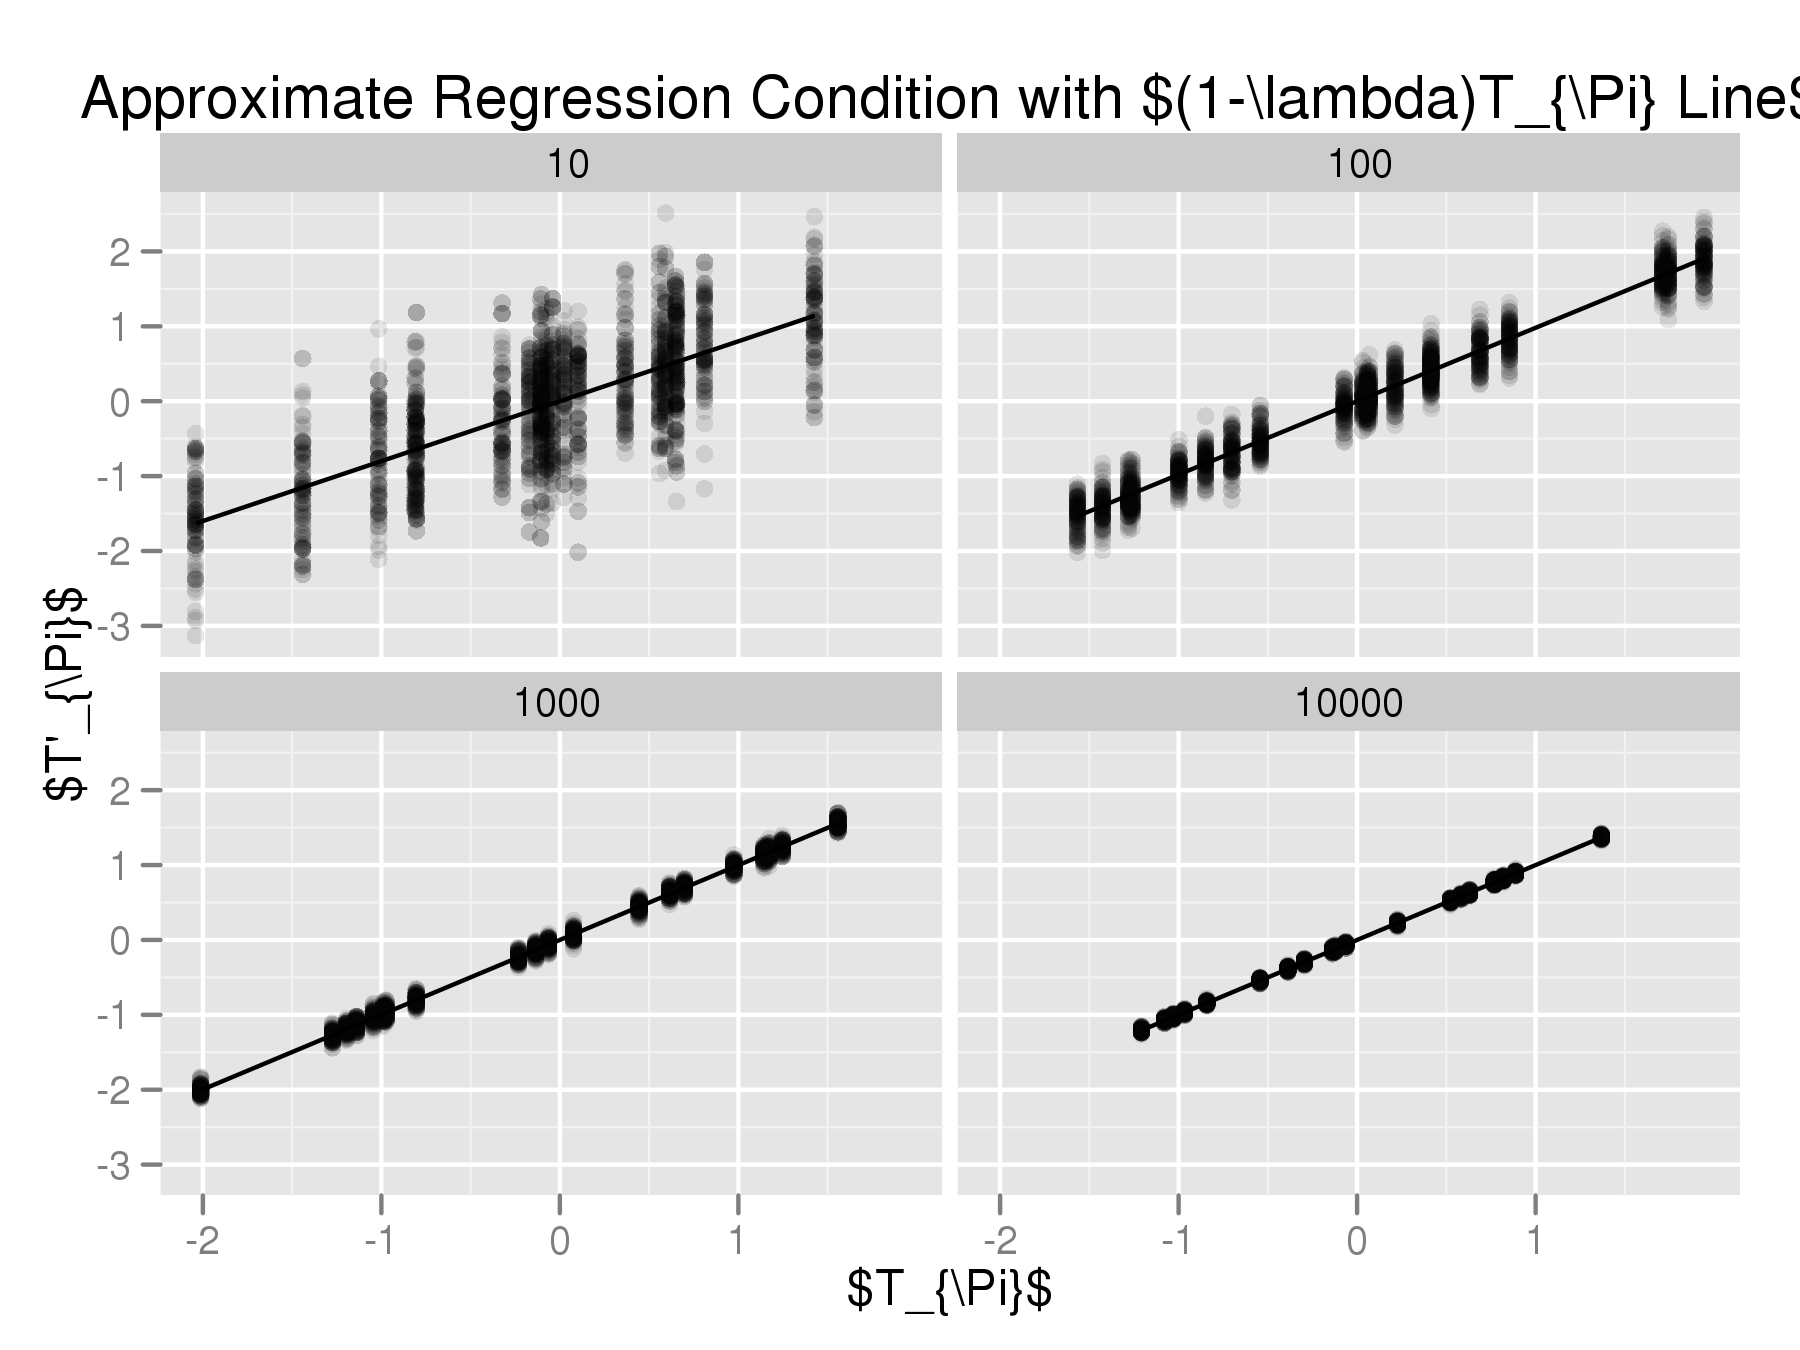
\includegraphics[scale = .75]{./simulations/sim7.png}
  \caption{Faceted on per-group sample size, $N$.}
\end{figure}

The approximate regression condition appears to hold visually.
\clearpage

\section{Main Bounds}
Here we simulate the main bounds under the same setting as the previous section.  
\subsection{Failure of Monte Carlo}
Again, we simulate the conditional expectations of the form $\E[f(T'_{\Pi}, T_{\Pi}) | T_{\Pi}]$
with 1,000 draws from the uniform distribution on all group-switching transpositions $(I, J)$.

\begin{figure}[!ht]
  \centering
  % Created by tikzDevice version 0.6.2 on 2012-04-24 14:14:48
% !TEX encoding = UTF-8 Unicode
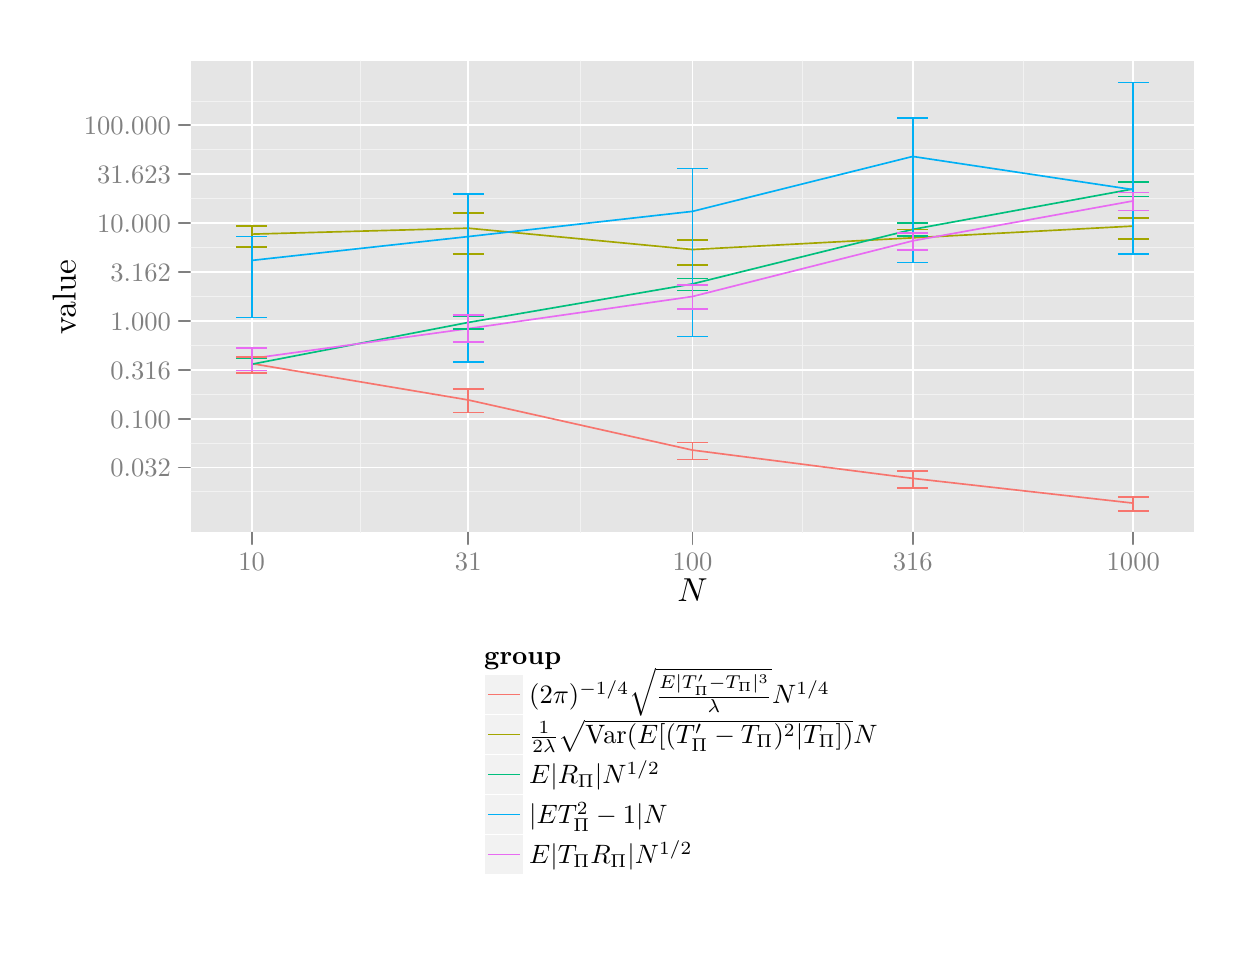
\begin{tikzpicture}[x=1pt,y=1pt]
\definecolor[named]{drawColor}{rgb}{0.00,0.00,0.00}
\definecolor[named]{fillColor}{rgb}{1.00,1.00,1.00}
\fill[color=fillColor,fill opacity=0.00,] (0,0) rectangle (433.62,325.21);
\begin{scope}
\path[clip] (  0.00,  0.00) rectangle (433.62,325.21);
\definecolor[named]{drawColor}{rgb}{0.41,0.16,0.58}
\end{scope}
\begin{scope}
\path[clip] (  0.00,  0.00) rectangle (433.62,325.21);
\definecolor[named]{drawColor}{rgb}{0.41,0.16,0.58}
\end{scope}
\begin{scope}
\path[clip] (  0.00,  0.00) rectangle (433.62,325.21);
\definecolor[named]{drawColor}{rgb}{0.41,0.16,0.58}
\end{scope}
\begin{scope}
\path[clip] (  0.00,  0.00) rectangle (433.62,325.21);
\definecolor[named]{drawColor}{rgb}{0.41,0.16,0.58}
\end{scope}
\begin{scope}
\path[clip] (  0.00,  0.00) rectangle (433.62,325.21);
\definecolor[named]{drawColor}{rgb}{0.41,0.16,0.58}
\end{scope}
\begin{scope}
\path[clip] (  0.00,  0.00) rectangle (433.62,325.21);
\definecolor[named]{drawColor}{rgb}{0.41,0.16,0.58}
\end{scope}
\begin{scope}
\path[clip] (  0.00,  0.00) rectangle (433.62,325.21);
\definecolor[named]{drawColor}{rgb}{0.41,0.16,0.58}
\end{scope}
\begin{scope}
\path[clip] (  0.00,  0.00) rectangle (433.62,325.21);
\definecolor[named]{drawColor}{rgb}{0.41,0.16,0.58}
\end{scope}
\begin{scope}
\path[clip] (  0.00,  0.00) rectangle (433.62,325.21);
\definecolor[named]{drawColor}{rgb}{0.41,0.16,0.58}
\end{scope}
\begin{scope}
\path[clip] (  0.00,  0.00) rectangle (433.62,325.21);
\definecolor[named]{drawColor}{rgb}{0.41,0.16,0.58}
\end{scope}
\begin{scope}
\path[clip] (  0.00,  0.00) rectangle (433.62,325.21);
\definecolor[named]{drawColor}{rgb}{0.41,0.16,0.58}
\end{scope}
\begin{scope}
\path[clip] (  0.00,  0.00) rectangle (433.62,325.21);
\definecolor[named]{drawColor}{rgb}{0.41,0.16,0.58}
\end{scope}
\begin{scope}
\path[clip] ( 58.88,142.81) rectangle (421.57,313.17);
\definecolor[named]{drawColor}{rgb}{0.41,0.16,0.58}
\end{scope}
\begin{scope}
\path[clip] (  0.00,  0.00) rectangle (433.62,325.21);
\definecolor[named]{drawColor}{rgb}{0.41,0.16,0.58}
\end{scope}
\begin{scope}
\path[clip] (  0.00,  0.00) rectangle (433.62,325.21);
\definecolor[named]{drawColor}{rgb}{0.41,0.16,0.58}
\end{scope}
\begin{scope}
\path[clip] (  0.00,  0.00) rectangle (433.62,325.21);
\definecolor[named]{drawColor}{rgb}{0.41,0.16,0.58}
\end{scope}
\begin{scope}
\path[clip] (  0.00,  0.00) rectangle (433.62,325.21);
\definecolor[named]{drawColor}{rgb}{0.41,0.16,0.58}
\end{scope}
\begin{scope}
\path[clip] (  0.00,  0.00) rectangle (433.62,325.21);
\definecolor[named]{drawColor}{rgb}{0.41,0.16,0.58}
\end{scope}
\begin{scope}
\path[clip] (  0.00,  0.00) rectangle (433.62,325.21);
\definecolor[named]{drawColor}{rgb}{0.41,0.16,0.58}
\end{scope}
\begin{scope}
\path[clip] (  0.00,  0.00) rectangle (433.62,325.21);
\definecolor[named]{drawColor}{rgb}{0.41,0.16,0.58}
\end{scope}
\begin{scope}
\path[clip] (  0.00,  0.00) rectangle (433.62,325.21);
\definecolor[named]{drawColor}{rgb}{0.41,0.16,0.58}
\end{scope}
\begin{scope}
\path[clip] (  0.00,  0.00) rectangle (433.62,325.21);
\definecolor[named]{drawColor}{rgb}{0.41,0.16,0.58}
\end{scope}
\begin{scope}
\path[clip] (  0.00,  0.00) rectangle (433.62,325.21);
\definecolor[named]{drawColor}{rgb}{0.41,0.16,0.58}
\end{scope}
\begin{scope}
\path[clip] (  0.00,  0.00) rectangle (433.62,325.21);
\definecolor[named]{drawColor}{rgb}{0.41,0.16,0.58}
\end{scope}
\begin{scope}
\path[clip] (  0.00,  0.00) rectangle (433.62,325.21);
\definecolor[named]{drawColor}{rgb}{0.41,0.16,0.58}
\definecolor[named]{fillColor}{rgb}{1.00,1.00,1.00}

\draw[fill=fillColor,draw opacity=0.00,] (  0.00,  0.00) rectangle (433.62,325.21);
\end{scope}
\begin{scope}
\path[clip] (  0.00,  0.00) rectangle (433.62,325.21);
\definecolor[named]{drawColor}{rgb}{0.41,0.16,0.58}
\end{scope}
\begin{scope}
\path[clip] (  0.00,  0.00) rectangle (433.62,325.21);
\definecolor[named]{drawColor}{rgb}{0.41,0.16,0.58}
\definecolor[named]{drawColor}{rgb}{0.50,0.50,0.50}

\node[color=drawColor,anchor=base east,inner sep=0pt, outer sep=0pt, scale=  0.96] at ( 51.77,162.98) {0.032};

\node[color=drawColor,anchor=base east,inner sep=0pt, outer sep=0pt, scale=  0.96] at ( 51.77,180.48) {0.100};

\node[color=drawColor,anchor=base east,inner sep=0pt, outer sep=0pt, scale=  0.96] at ( 51.77,198.16) {0.316};

\node[color=drawColor,anchor=base east,inner sep=0pt, outer sep=0pt, scale=  0.96] at ( 51.77,215.86) {1.000};

\node[color=drawColor,anchor=base east,inner sep=0pt, outer sep=0pt, scale=  0.96] at ( 51.77,233.55) {3.162};

\node[color=drawColor,anchor=base east,inner sep=0pt, outer sep=0pt, scale=  0.96] at ( 51.77,251.23) {10.000};

\node[color=drawColor,anchor=base east,inner sep=0pt, outer sep=0pt, scale=  0.96] at ( 51.77,268.92) {31.623};

\node[color=drawColor,anchor=base east,inner sep=0pt, outer sep=0pt, scale=  0.96] at ( 51.77,286.61) {100.000};
\end{scope}
\begin{scope}
\path[clip] (  0.00,  0.00) rectangle (433.62,325.21);
\definecolor[named]{drawColor}{rgb}{0.41,0.16,0.58}
\definecolor[named]{drawColor}{rgb}{0.50,0.50,0.50}

\draw[color=drawColor,line width= 0.6pt,line cap=round,line join=round,fill opacity=0.00,] ( 54.61,166.28) -- ( 58.88,166.28);

\draw[color=drawColor,line width= 0.6pt,line cap=round,line join=round,fill opacity=0.00,] ( 54.61,183.79) -- ( 58.88,183.79);

\draw[color=drawColor,line width= 0.6pt,line cap=round,line join=round,fill opacity=0.00,] ( 54.61,201.46) -- ( 58.88,201.46);

\draw[color=drawColor,line width= 0.6pt,line cap=round,line join=round,fill opacity=0.00,] ( 54.61,219.16) -- ( 58.88,219.16);

\draw[color=drawColor,line width= 0.6pt,line cap=round,line join=round,fill opacity=0.00,] ( 54.61,236.85) -- ( 58.88,236.85);

\draw[color=drawColor,line width= 0.6pt,line cap=round,line join=round,fill opacity=0.00,] ( 54.61,254.54) -- ( 58.88,254.54);

\draw[color=drawColor,line width= 0.6pt,line cap=round,line join=round,fill opacity=0.00,] ( 54.61,272.23) -- ( 58.88,272.23);

\draw[color=drawColor,line width= 0.6pt,line cap=round,line join=round,fill opacity=0.00,] ( 54.61,289.92) -- ( 58.88,289.92);
\end{scope}
\begin{scope}
\path[clip] (  0.00,  0.00) rectangle (433.62,325.21);
\definecolor[named]{drawColor}{rgb}{0.41,0.16,0.58}
\end{scope}
\begin{scope}
\path[clip] (  0.00,  0.00) rectangle (433.62,325.21);
\definecolor[named]{drawColor}{rgb}{0.41,0.16,0.58}
\end{scope}
\begin{scope}
\path[clip] (  0.00,  0.00) rectangle (433.62,325.21);
\definecolor[named]{drawColor}{rgb}{0.41,0.16,0.58}
\end{scope}
\begin{scope}
\path[clip] (  0.00,  0.00) rectangle (433.62,325.21);
\definecolor[named]{drawColor}{rgb}{0.41,0.16,0.58}
\end{scope}
\begin{scope}
\path[clip] (  0.00,  0.00) rectangle (433.62,325.21);
\definecolor[named]{drawColor}{rgb}{0.41,0.16,0.58}
\end{scope}
\begin{scope}
\path[clip] ( 58.88,142.81) rectangle (421.57,313.17);
\definecolor[named]{drawColor}{rgb}{0.41,0.16,0.58}
\definecolor[named]{fillColor}{rgb}{0.90,0.90,0.90}

\draw[fill=fillColor,draw opacity=0.00,] ( 58.88,142.81) rectangle (421.57,313.17);
\definecolor[named]{drawColor}{rgb}{0.95,0.95,0.95}

\draw[color=drawColor,line width= 0.3pt,line cap=round,line join=round,fill opacity=0.00,] ( 58.88,157.53) --
	(421.57,157.53);

\draw[color=drawColor,line width= 0.3pt,line cap=round,line join=round,fill opacity=0.00,] ( 58.88,175.03) --
	(421.57,175.03);

\draw[color=drawColor,line width= 0.3pt,line cap=round,line join=round,fill opacity=0.00,] ( 58.88,192.63) --
	(421.57,192.63);

\draw[color=drawColor,line width= 0.3pt,line cap=round,line join=round,fill opacity=0.00,] ( 58.88,210.31) --
	(421.57,210.31);

\draw[color=drawColor,line width= 0.3pt,line cap=round,line join=round,fill opacity=0.00,] ( 58.88,228.01) --
	(421.57,228.01);

\draw[color=drawColor,line width= 0.3pt,line cap=round,line join=round,fill opacity=0.00,] ( 58.88,245.70) --
	(421.57,245.70);

\draw[color=drawColor,line width= 0.3pt,line cap=round,line join=round,fill opacity=0.00,] ( 58.88,263.38) --
	(421.57,263.38);

\draw[color=drawColor,line width= 0.3pt,line cap=round,line join=round,fill opacity=0.00,] ( 58.88,281.07) --
	(421.57,281.07);

\draw[color=drawColor,line width= 0.3pt,line cap=round,line join=round,fill opacity=0.00,] ( 58.88,298.67) --
	(421.57,298.67);

\draw[color=drawColor,line width= 0.3pt,line cap=round,line join=round,fill opacity=0.00,] (120.08,142.81) --
	(120.08,313.17);

\draw[color=drawColor,line width= 0.3pt,line cap=round,line join=round,fill opacity=0.00,] (199.72,142.81) --
	(199.72,313.17);

\draw[color=drawColor,line width= 0.3pt,line cap=round,line join=round,fill opacity=0.00,] (280.02,142.81) --
	(280.02,313.17);

\draw[color=drawColor,line width= 0.3pt,line cap=round,line join=round,fill opacity=0.00,] (359.67,142.81) --
	(359.67,313.17);
\definecolor[named]{drawColor}{rgb}{1.00,1.00,1.00}

\draw[color=drawColor,line width= 0.6pt,line cap=round,line join=round,fill opacity=0.00,] ( 58.88,166.28) --
	(421.57,166.28);

\draw[color=drawColor,line width= 0.6pt,line cap=round,line join=round,fill opacity=0.00,] ( 58.88,183.79) --
	(421.57,183.79);

\draw[color=drawColor,line width= 0.6pt,line cap=round,line join=round,fill opacity=0.00,] ( 58.88,201.46) --
	(421.57,201.46);

\draw[color=drawColor,line width= 0.6pt,line cap=round,line join=round,fill opacity=0.00,] ( 58.88,219.16) --
	(421.57,219.16);

\draw[color=drawColor,line width= 0.6pt,line cap=round,line join=round,fill opacity=0.00,] ( 58.88,236.85) --
	(421.57,236.85);

\draw[color=drawColor,line width= 0.6pt,line cap=round,line join=round,fill opacity=0.00,] ( 58.88,254.54) --
	(421.57,254.54);

\draw[color=drawColor,line width= 0.6pt,line cap=round,line join=round,fill opacity=0.00,] ( 58.88,272.23) --
	(421.57,272.23);

\draw[color=drawColor,line width= 0.6pt,line cap=round,line join=round,fill opacity=0.00,] ( 58.88,289.92) --
	(421.57,289.92);

\draw[color=drawColor,line width= 0.6pt,line cap=round,line join=round,fill opacity=0.00,] ( 80.94,142.81) --
	( 80.94,313.17);

\draw[color=drawColor,line width= 0.6pt,line cap=round,line join=round,fill opacity=0.00,] (159.21,142.81) --
	(159.21,313.17);

\draw[color=drawColor,line width= 0.6pt,line cap=round,line join=round,fill opacity=0.00,] (240.23,142.81) --
	(240.23,313.17);

\draw[color=drawColor,line width= 0.6pt,line cap=round,line join=round,fill opacity=0.00,] (319.82,142.81) --
	(319.82,313.17);

\draw[color=drawColor,line width= 0.6pt,line cap=round,line join=round,fill opacity=0.00,] (399.51,142.81) --
	(399.51,313.17);
\definecolor[named]{drawColor}{rgb}{0.97,0.46,0.43}

\draw[color=drawColor,line width= 0.6pt,line join=round,fill opacity=0.00,] ( 80.94,203.83) --
	(159.21,190.68) --
	(240.23,172.56) --
	(319.82,162.35) --
	(399.51,153.40);
\definecolor[named]{drawColor}{rgb}{0.64,0.65,0.00}

\draw[color=drawColor,line width= 0.6pt,line join=round,fill opacity=0.00,] ( 80.94,250.60) --
	(159.21,252.75) --
	(240.23,245.03) --
	(319.82,249.27) --
	(399.51,253.51);
\definecolor[named]{drawColor}{rgb}{0.00,0.75,0.49}

\draw[color=drawColor,line width= 0.6pt,line join=round,fill opacity=0.00,] ( 80.94,203.59) --
	(159.21,218.69) --
	(240.23,232.62) --
	(319.82,252.32) --
	(399.51,266.94);
\definecolor[named]{drawColor}{rgb}{0.00,0.69,0.96}

\draw[color=drawColor,line width= 0.6pt,line join=round,fill opacity=0.00,] ( 80.94,241.10) --
	(159.21,249.72) --
	(240.23,258.83) --
	(319.82,278.67) --
	(399.51,266.67);
\definecolor[named]{drawColor}{rgb}{0.91,0.42,0.95}

\draw[color=drawColor,line width= 0.6pt,line join=round,fill opacity=0.00,] ( 80.94,205.66) --
	(159.21,216.47) --
	(240.23,228.06) --
	(319.82,248.18) --
	(399.51,262.61);
\definecolor[named]{drawColor}{rgb}{0.97,0.46,0.43}

\draw[color=drawColor,line width= 0.6pt,line join=round,fill opacity=0.00,] ( 75.37,206.32) --
	( 86.52,206.32);

\draw[color=drawColor,line width= 0.6pt,line join=round,fill opacity=0.00,] ( 80.94,206.32) --
	( 80.94,200.34);

\draw[color=drawColor,line width= 0.6pt,line join=round,fill opacity=0.00,] ( 75.37,200.34) --
	( 86.52,200.34);

\draw[color=drawColor,line width= 0.6pt,line join=round,fill opacity=0.00,] (153.63,194.68) --
	(164.78,194.68);

\draw[color=drawColor,line width= 0.6pt,line join=round,fill opacity=0.00,] (159.21,194.68) --
	(159.21,186.16);

\draw[color=drawColor,line width= 0.6pt,line join=round,fill opacity=0.00,] (153.63,186.16) --
	(164.78,186.16);

\draw[color=drawColor,line width= 0.6pt,line join=round,fill opacity=0.00,] (234.65,175.26) --
	(245.80,175.26);

\draw[color=drawColor,line width= 0.6pt,line join=round,fill opacity=0.00,] (240.23,175.26) --
	(240.23,169.21);

\draw[color=drawColor,line width= 0.6pt,line join=round,fill opacity=0.00,] (234.65,169.21) --
	(245.80,169.21);

\draw[color=drawColor,line width= 0.6pt,line join=round,fill opacity=0.00,] (314.25,165.12) --
	(325.40,165.12);

\draw[color=drawColor,line width= 0.6pt,line join=round,fill opacity=0.00,] (319.82,165.12) --
	(319.82,158.87);

\draw[color=drawColor,line width= 0.6pt,line join=round,fill opacity=0.00,] (314.25,158.87) --
	(325.40,158.87);

\draw[color=drawColor,line width= 0.6pt,line join=round,fill opacity=0.00,] (393.94,155.69) --
	(405.09,155.69);

\draw[color=drawColor,line width= 0.6pt,line join=round,fill opacity=0.00,] (399.51,155.69) --
	(399.51,150.56);

\draw[color=drawColor,line width= 0.6pt,line join=round,fill opacity=0.00,] (393.94,150.56) --
	(405.09,150.56);
\definecolor[named]{drawColor}{rgb}{0.64,0.65,0.00}

\draw[color=drawColor,line width= 0.6pt,line join=round,fill opacity=0.00,] ( 75.37,253.47) --
	( 86.52,253.47);

\draw[color=drawColor,line width= 0.6pt,line join=round,fill opacity=0.00,] ( 80.94,253.47) --
	( 80.94,245.96);

\draw[color=drawColor,line width= 0.6pt,line join=round,fill opacity=0.00,] ( 75.37,245.96) --
	( 86.52,245.96);

\draw[color=drawColor,line width= 0.6pt,line join=round,fill opacity=0.00,] (153.63,258.32) --
	(164.78,258.32);

\draw[color=drawColor,line width= 0.6pt,line join=round,fill opacity=0.00,] (159.21,258.32) --
	(159.21,243.44);

\draw[color=drawColor,line width= 0.6pt,line join=round,fill opacity=0.00,] (153.63,243.44) --
	(164.78,243.44);

\draw[color=drawColor,line width= 0.6pt,line join=round,fill opacity=0.00,] (234.65,248.50) --
	(245.80,248.50);

\draw[color=drawColor,line width= 0.6pt,line join=round,fill opacity=0.00,] (240.23,248.50) --
	(240.23,239.42);

\draw[color=drawColor,line width= 0.6pt,line join=round,fill opacity=0.00,] (234.65,239.42) --
	(245.80,239.42);

\draw[color=drawColor,line width= 0.6pt,line join=round,fill opacity=0.00,] (314.25,252.27) --
	(325.40,252.27);

\draw[color=drawColor,line width= 0.6pt,line join=round,fill opacity=0.00,] (319.82,252.27) --
	(319.82,244.74);

\draw[color=drawColor,line width= 0.6pt,line join=round,fill opacity=0.00,] (314.25,244.74) --
	(325.40,244.74);

\draw[color=drawColor,line width= 0.6pt,line join=round,fill opacity=0.00,] (393.94,256.44) --
	(405.09,256.44);

\draw[color=drawColor,line width= 0.6pt,line join=round,fill opacity=0.00,] (399.51,256.44) --
	(399.51,248.83);

\draw[color=drawColor,line width= 0.6pt,line join=round,fill opacity=0.00,] (393.94,248.83) --
	(405.09,248.83);
\definecolor[named]{drawColor}{rgb}{0.00,0.75,0.49}

\draw[color=drawColor,line width= 0.6pt,line join=round,fill opacity=0.00,] ( 75.37,205.70) --
	( 86.52,205.70);

\draw[color=drawColor,line width= 0.6pt,line join=round,fill opacity=0.00,] ( 80.94,205.70) --
	( 80.94,201.35);

\draw[color=drawColor,line width= 0.6pt,line join=round,fill opacity=0.00,] ( 75.37,201.35) --
	( 86.52,201.35);

\draw[color=drawColor,line width= 0.6pt,line join=round,fill opacity=0.00,] (153.63,220.88) --
	(164.78,220.88);

\draw[color=drawColor,line width= 0.6pt,line join=round,fill opacity=0.00,] (159.21,220.88) --
	(159.21,216.35);

\draw[color=drawColor,line width= 0.6pt,line join=round,fill opacity=0.00,] (153.63,216.35) --
	(164.78,216.35);

\draw[color=drawColor,line width= 0.6pt,line join=round,fill opacity=0.00,] (234.65,234.62) --
	(245.80,234.62);

\draw[color=drawColor,line width= 0.6pt,line join=round,fill opacity=0.00,] (240.23,234.62) --
	(240.23,230.23);

\draw[color=drawColor,line width= 0.6pt,line join=round,fill opacity=0.00,] (234.65,230.23) --
	(245.80,230.23);

\draw[color=drawColor,line width= 0.6pt,line join=round,fill opacity=0.00,] (314.25,254.55) --
	(325.40,254.55);

\draw[color=drawColor,line width= 0.6pt,line join=round,fill opacity=0.00,] (319.82,254.55) --
	(319.82,249.92);

\draw[color=drawColor,line width= 0.6pt,line join=round,fill opacity=0.00,] (314.25,249.92) --
	(325.40,249.92);

\draw[color=drawColor,line width= 0.6pt,line join=round,fill opacity=0.00,] (393.94,269.37) --
	(405.09,269.37);

\draw[color=drawColor,line width= 0.6pt,line join=round,fill opacity=0.00,] (399.51,269.37) --
	(399.51,264.26);

\draw[color=drawColor,line width= 0.6pt,line join=round,fill opacity=0.00,] (393.94,264.26) --
	(405.09,264.26);
\definecolor[named]{drawColor}{rgb}{0.00,0.69,0.96}

\draw[color=drawColor,line width= 0.6pt,line join=round,fill opacity=0.00,] ( 75.37,249.80) --
	( 86.52,249.80);

\draw[color=drawColor,line width= 0.6pt,line join=round,fill opacity=0.00,] ( 80.94,249.80) --
	( 80.94,220.53);

\draw[color=drawColor,line width= 0.6pt,line join=round,fill opacity=0.00,] ( 75.37,220.53) --
	( 86.52,220.53);

\draw[color=drawColor,line width= 0.6pt,line join=round,fill opacity=0.00,] (153.63,265.15) --
	(164.78,265.15);

\draw[color=drawColor,line width= 0.6pt,line join=round,fill opacity=0.00,] (159.21,265.15) --
	(159.21,204.45);

\draw[color=drawColor,line width= 0.6pt,line join=round,fill opacity=0.00,] (153.63,204.45) --
	(164.78,204.45);

\draw[color=drawColor,line width= 0.6pt,line join=round,fill opacity=0.00,] (234.65,274.32) --
	(245.80,274.32);

\draw[color=drawColor,line width= 0.6pt,line join=round,fill opacity=0.00,] (240.23,274.32) --
	(240.23,213.60);

\draw[color=drawColor,line width= 0.6pt,line join=round,fill opacity=0.00,] (234.65,213.60) --
	(245.80,213.60);

\draw[color=drawColor,line width= 0.6pt,line join=round,fill opacity=0.00,] (314.25,292.55) --
	(325.40,292.55);

\draw[color=drawColor,line width= 0.6pt,line join=round,fill opacity=0.00,] (319.82,292.55) --
	(319.82,240.36);

\draw[color=drawColor,line width= 0.6pt,line join=round,fill opacity=0.00,] (314.25,240.36) --
	(325.40,240.36);

\draw[color=drawColor,line width= 0.6pt,line join=round,fill opacity=0.00,] (393.94,305.43) --
	(405.09,305.43);

\draw[color=drawColor,line width= 0.6pt,line join=round,fill opacity=0.00,] (399.51,305.43) --
	(399.51,243.53);

\draw[color=drawColor,line width= 0.6pt,line join=round,fill opacity=0.00,] (393.94,243.53) --
	(405.09,243.53);
\definecolor[named]{drawColor}{rgb}{0.91,0.42,0.95}

\draw[color=drawColor,line width= 0.6pt,line join=round,fill opacity=0.00,] ( 75.37,209.42) --
	( 86.52,209.42);

\draw[color=drawColor,line width= 0.6pt,line join=round,fill opacity=0.00,] ( 80.94,209.42) --
	( 80.94,201.38);

\draw[color=drawColor,line width= 0.6pt,line join=round,fill opacity=0.00,] ( 75.37,201.38) --
	( 86.52,201.38);

\draw[color=drawColor,line width= 0.6pt,line join=round,fill opacity=0.00,] (153.63,221.29) --
	(164.78,221.29);

\draw[color=drawColor,line width= 0.6pt,line join=round,fill opacity=0.00,] (159.21,221.29) --
	(159.21,211.56);

\draw[color=drawColor,line width= 0.6pt,line join=round,fill opacity=0.00,] (153.63,211.56) --
	(164.78,211.56);

\draw[color=drawColor,line width= 0.6pt,line join=round,fill opacity=0.00,] (234.65,232.16) --
	(245.80,232.16);

\draw[color=drawColor,line width= 0.6pt,line join=round,fill opacity=0.00,] (240.23,232.16) --
	(240.23,223.62);

\draw[color=drawColor,line width= 0.6pt,line join=round,fill opacity=0.00,] (234.65,223.62) --
	(245.80,223.62);

\draw[color=drawColor,line width= 0.6pt,line join=round,fill opacity=0.00,] (314.25,251.01) --
	(325.40,251.01);

\draw[color=drawColor,line width= 0.6pt,line join=round,fill opacity=0.00,] (319.82,251.01) --
	(319.82,244.79);

\draw[color=drawColor,line width= 0.6pt,line join=round,fill opacity=0.00,] (314.25,244.79) --
	(325.40,244.79);

\draw[color=drawColor,line width= 0.6pt,line join=round,fill opacity=0.00,] (393.94,265.59) --
	(405.09,265.59);

\draw[color=drawColor,line width= 0.6pt,line join=round,fill opacity=0.00,] (399.51,265.59) --
	(399.51,259.13);

\draw[color=drawColor,line width= 0.6pt,line join=round,fill opacity=0.00,] (393.94,259.13) --
	(405.09,259.13);
\end{scope}
\begin{scope}
\path[clip] (  0.00,  0.00) rectangle (433.62,325.21);
\definecolor[named]{drawColor}{rgb}{0.41,0.16,0.58}
\end{scope}
\begin{scope}
\path[clip] (  0.00,  0.00) rectangle (433.62,325.21);
\definecolor[named]{drawColor}{rgb}{0.41,0.16,0.58}
\definecolor[named]{drawColor}{rgb}{0.50,0.50,0.50}

\node[color=drawColor,anchor=base,inner sep=0pt, outer sep=0pt, scale=  0.96] at ( 80.94,129.09) {10};

\node[color=drawColor,anchor=base,inner sep=0pt, outer sep=0pt, scale=  0.96] at (159.21,129.09) {31};

\node[color=drawColor,anchor=base,inner sep=0pt, outer sep=0pt, scale=  0.96] at (240.23,129.09) {100};

\node[color=drawColor,anchor=base,inner sep=0pt, outer sep=0pt, scale=  0.96] at (319.82,129.09) {316};

\node[color=drawColor,anchor=base,inner sep=0pt, outer sep=0pt, scale=  0.96] at (399.51,129.09) {1000};
\end{scope}
\begin{scope}
\path[clip] (  0.00,  0.00) rectangle (433.62,325.21);
\definecolor[named]{drawColor}{rgb}{0.41,0.16,0.58}
\definecolor[named]{drawColor}{rgb}{0.50,0.50,0.50}

\draw[color=drawColor,line width= 0.6pt,line cap=round,line join=round,fill opacity=0.00,] ( 80.94,138.55) -- ( 80.94,142.81);

\draw[color=drawColor,line width= 0.6pt,line cap=round,line join=round,fill opacity=0.00,] (159.21,138.55) -- (159.21,142.81);

\draw[color=drawColor,line width= 0.6pt,line cap=round,line join=round,fill opacity=0.00,] (240.23,138.55) -- (240.23,142.81);

\draw[color=drawColor,line width= 0.6pt,line cap=round,line join=round,fill opacity=0.00,] (319.82,138.55) -- (319.82,142.81);

\draw[color=drawColor,line width= 0.6pt,line cap=round,line join=round,fill opacity=0.00,] (399.51,138.55) -- (399.51,142.81);
\end{scope}
\begin{scope}
\path[clip] (  0.00,  0.00) rectangle (433.62,325.21);
\definecolor[named]{drawColor}{rgb}{0.41,0.16,0.58}
\end{scope}
\begin{scope}
\path[clip] (  0.00,  0.00) rectangle (433.62,325.21);
\definecolor[named]{drawColor}{rgb}{0.41,0.16,0.58}
\end{scope}
\begin{scope}
\path[clip] (  0.00,  0.00) rectangle (433.62,325.21);
\definecolor[named]{drawColor}{rgb}{0.41,0.16,0.58}
\end{scope}
\begin{scope}
\path[clip] (  0.00,  0.00) rectangle (433.62,325.21);
\definecolor[named]{drawColor}{rgb}{0.41,0.16,0.58}
\end{scope}
\begin{scope}
\path[clip] (  0.00,  0.00) rectangle (433.62,325.21);
\definecolor[named]{drawColor}{rgb}{0.41,0.16,0.58}
\end{scope}
\begin{scope}
\path[clip] (  0.00,  0.00) rectangle (433.62,325.21);
\definecolor[named]{drawColor}{rgb}{0.41,0.16,0.58}
\definecolor[named]{drawColor}{rgb}{0.00,0.00,0.00}

\node[color=drawColor,anchor=base,inner sep=0pt, outer sep=0pt, scale=  1.20] at (240.23,117.81) {$N$};
\end{scope}
\begin{scope}
\path[clip] (  0.00,  0.00) rectangle (433.62,325.21);
\definecolor[named]{drawColor}{rgb}{0.41,0.16,0.58}
\end{scope}
\begin{scope}
\path[clip] (  0.00,  0.00) rectangle (433.62,325.21);
\definecolor[named]{drawColor}{rgb}{0.41,0.16,0.58}
\definecolor[named]{drawColor}{rgb}{0.00,0.00,0.00}

\node[rotate= 90.00,color=drawColor,anchor=base,inner sep=0pt, outer sep=0pt, scale=  1.20] at ( 17.30,227.99) {value};
\end{scope}
\begin{scope}
\path[clip] (  0.00,  0.00) rectangle (433.62,325.21);
\definecolor[named]{drawColor}{rgb}{0.41,0.16,0.58}
\end{scope}
\begin{scope}
\path[clip] (  0.00,  0.00) rectangle (433.62,325.21);
\definecolor[named]{drawColor}{rgb}{0.41,0.16,0.58}
\end{scope}
\begin{scope}
\path[clip] (  0.00,  0.00) rectangle (433.62,325.21);
\definecolor[named]{drawColor}{rgb}{0.41,0.16,0.58}
\end{scope}
\begin{scope}
\path[clip] (  0.00,  0.00) rectangle (433.62,325.21);
\definecolor[named]{drawColor}{rgb}{0.41,0.16,0.58}
\end{scope}
\begin{scope}
\path[clip] (  0.00,  0.00) rectangle (433.62,325.21);
\definecolor[named]{drawColor}{rgb}{0.41,0.16,0.58}
\end{scope}
\begin{scope}
\path[clip] (  0.00,  0.00) rectangle (433.62,325.21);
\definecolor[named]{drawColor}{rgb}{0.41,0.16,0.58}
\end{scope}
\begin{scope}
\path[clip] (  0.00,  0.00) rectangle (433.62,325.21);
\definecolor[named]{drawColor}{rgb}{0.41,0.16,0.58}
\end{scope}
\begin{scope}
\path[clip] (  0.00,  0.00) rectangle (433.62,325.21);
\definecolor[named]{drawColor}{rgb}{0.41,0.16,0.58}
\end{scope}
\begin{scope}
\path[clip] (  0.00,  0.00) rectangle (433.62,325.21);
\definecolor[named]{drawColor}{rgb}{0.41,0.16,0.58}
\end{scope}
\begin{scope}
\path[clip] (  0.00,  0.00) rectangle (433.62,325.21);
\definecolor[named]{drawColor}{rgb}{0.41,0.16,0.58}
\end{scope}
\begin{scope}
\path[clip] (  0.00,  0.00) rectangle (433.62,325.21);
\definecolor[named]{drawColor}{rgb}{0.41,0.16,0.58}
\end{scope}
\begin{scope}
\path[clip] (  0.00,  0.00) rectangle (433.62,325.21);
\definecolor[named]{drawColor}{rgb}{0.41,0.16,0.58}
\end{scope}
\begin{scope}
\path[clip] (  0.00,  0.00) rectangle (433.62,325.21);
\definecolor[named]{drawColor}{rgb}{0.41,0.16,0.58}
\end{scope}
\begin{scope}
\path[clip] (  0.00,  0.00) rectangle (433.62,325.21);
\definecolor[named]{drawColor}{rgb}{0.41,0.16,0.58}
\end{scope}
\begin{scope}
\path[clip] (  0.00,  0.00) rectangle (433.62,325.21);
\definecolor[named]{drawColor}{rgb}{0.41,0.16,0.58}
\end{scope}
\begin{scope}
\path[clip] (  0.00,  0.00) rectangle (433.62,325.21);
\definecolor[named]{drawColor}{rgb}{0.41,0.16,0.58}
\end{scope}
\begin{scope}
\path[clip] (  0.00,  0.00) rectangle (433.62,325.21);
\definecolor[named]{drawColor}{rgb}{0.41,0.16,0.58}
\end{scope}
\begin{scope}
\path[clip] (  0.00,  0.00) rectangle (433.62,325.21);
\definecolor[named]{drawColor}{rgb}{0.41,0.16,0.58}
\end{scope}
\begin{scope}
\path[clip] (  0.00,  0.00) rectangle (433.62,325.21);
\definecolor[named]{drawColor}{rgb}{0.41,0.16,0.58}
\end{scope}
\begin{scope}
\path[clip] (  0.00,  0.00) rectangle (433.62,325.21);
\definecolor[named]{drawColor}{rgb}{0.41,0.16,0.58}
\end{scope}
\begin{scope}
\path[clip] (  0.00,  0.00) rectangle (433.62,325.21);
\definecolor[named]{drawColor}{rgb}{0.41,0.16,0.58}
\end{scope}
\begin{scope}
\path[clip] (  0.00,  0.00) rectangle (433.62,325.21);
\definecolor[named]{drawColor}{rgb}{0.41,0.16,0.58}
\end{scope}
\begin{scope}
\path[clip] (  0.00,  0.00) rectangle (433.62,325.21);
\definecolor[named]{drawColor}{rgb}{0.41,0.16,0.58}
\end{scope}
\begin{scope}
\path[clip] (  0.00,  0.00) rectangle (433.62,325.21);
\definecolor[named]{drawColor}{rgb}{0.41,0.16,0.58}
\end{scope}
\begin{scope}
\path[clip] (  0.00,  0.00) rectangle (433.62,325.21);
\definecolor[named]{drawColor}{rgb}{0.41,0.16,0.58}
\definecolor[named]{drawColor}{rgb}{1.00,1.00,1.00}

\draw[color=drawColor,line width= 0.6pt,line cap=round,line join=round,fill opacity=0.00,] (160.71, 14.89) rectangle (319.75,105.93);
\end{scope}
\begin{scope}
\path[clip] (  0.00,  0.00) rectangle (433.62,325.21);
\definecolor[named]{drawColor}{rgb}{0.41,0.16,0.58}
\definecolor[named]{drawColor}{rgb}{0.00,0.00,0.00}

\node[color=drawColor,anchor=base west,inner sep=0pt, outer sep=0pt, scale=  0.96] at (164.98, 95.04) {\bfseries group};
\end{scope}
\begin{scope}
\path[clip] (  0.00,  0.00) rectangle (433.62,325.21);
\definecolor[named]{drawColor}{rgb}{0.41,0.16,0.58}
\definecolor[named]{drawColor}{rgb}{1.00,1.00,1.00}
\definecolor[named]{fillColor}{rgb}{0.95,0.95,0.95}

\draw[color=drawColor,line width= 0.6pt,line cap=round,line join=round,fill=fillColor,] (164.98, 76.97) rectangle (179.43, 91.43);
\end{scope}
\begin{scope}
\path[clip] (  0.00,  0.00) rectangle (433.62,325.21);
\definecolor[named]{drawColor}{rgb}{0.41,0.16,0.58}
\definecolor[named]{drawColor}{rgb}{0.97,0.46,0.43}

\draw[color=drawColor,line width= 0.6pt,line join=round,fill opacity=0.00,] (166.42, 84.20) -- (177.98, 84.20);
\end{scope}
\begin{scope}
\path[clip] (  0.00,  0.00) rectangle (433.62,325.21);
\definecolor[named]{drawColor}{rgb}{0.41,0.16,0.58}
\definecolor[named]{drawColor}{rgb}{0.97,0.46,0.43}

\draw[color=drawColor,line width= 0.6pt,line join=round,fill opacity=0.00,] (166.42, 84.20) -- (177.98, 84.20);
\end{scope}
\begin{scope}
\path[clip] (  0.00,  0.00) rectangle (433.62,325.21);
\definecolor[named]{drawColor}{rgb}{0.41,0.16,0.58}
\definecolor[named]{drawColor}{rgb}{1.00,1.00,1.00}
\definecolor[named]{fillColor}{rgb}{0.95,0.95,0.95}

\draw[color=drawColor,line width= 0.6pt,line cap=round,line join=round,fill=fillColor,] (164.98, 62.52) rectangle (179.43, 76.97);
\end{scope}
\begin{scope}
\path[clip] (  0.00,  0.00) rectangle (433.62,325.21);
\definecolor[named]{drawColor}{rgb}{0.41,0.16,0.58}
\definecolor[named]{drawColor}{rgb}{0.64,0.65,0.00}

\draw[color=drawColor,line width= 0.6pt,line join=round,fill opacity=0.00,] (166.42, 69.75) -- (177.98, 69.75);
\end{scope}
\begin{scope}
\path[clip] (  0.00,  0.00) rectangle (433.62,325.21);
\definecolor[named]{drawColor}{rgb}{0.41,0.16,0.58}
\definecolor[named]{drawColor}{rgb}{0.64,0.65,0.00}

\draw[color=drawColor,line width= 0.6pt,line join=round,fill opacity=0.00,] (166.42, 69.75) -- (177.98, 69.75);
\end{scope}
\begin{scope}
\path[clip] (  0.00,  0.00) rectangle (433.62,325.21);
\definecolor[named]{drawColor}{rgb}{0.41,0.16,0.58}
\definecolor[named]{drawColor}{rgb}{1.00,1.00,1.00}
\definecolor[named]{fillColor}{rgb}{0.95,0.95,0.95}

\draw[color=drawColor,line width= 0.6pt,line cap=round,line join=round,fill=fillColor,] (164.98, 48.07) rectangle (179.43, 62.52);
\end{scope}
\begin{scope}
\path[clip] (  0.00,  0.00) rectangle (433.62,325.21);
\definecolor[named]{drawColor}{rgb}{0.41,0.16,0.58}
\definecolor[named]{drawColor}{rgb}{0.00,0.75,0.49}

\draw[color=drawColor,line width= 0.6pt,line join=round,fill opacity=0.00,] (166.42, 55.29) -- (177.98, 55.29);
\end{scope}
\begin{scope}
\path[clip] (  0.00,  0.00) rectangle (433.62,325.21);
\definecolor[named]{drawColor}{rgb}{0.41,0.16,0.58}
\definecolor[named]{drawColor}{rgb}{0.00,0.75,0.49}

\draw[color=drawColor,line width= 0.6pt,line join=round,fill opacity=0.00,] (166.42, 55.29) -- (177.98, 55.29);
\end{scope}
\begin{scope}
\path[clip] (  0.00,  0.00) rectangle (433.62,325.21);
\definecolor[named]{drawColor}{rgb}{0.41,0.16,0.58}
\definecolor[named]{drawColor}{rgb}{1.00,1.00,1.00}
\definecolor[named]{fillColor}{rgb}{0.95,0.95,0.95}

\draw[color=drawColor,line width= 0.6pt,line cap=round,line join=round,fill=fillColor,] (164.98, 33.61) rectangle (179.43, 48.07);
\end{scope}
\begin{scope}
\path[clip] (  0.00,  0.00) rectangle (433.62,325.21);
\definecolor[named]{drawColor}{rgb}{0.41,0.16,0.58}
\definecolor[named]{drawColor}{rgb}{0.00,0.69,0.96}

\draw[color=drawColor,line width= 0.6pt,line join=round,fill opacity=0.00,] (166.42, 40.84) -- (177.98, 40.84);
\end{scope}
\begin{scope}
\path[clip] (  0.00,  0.00) rectangle (433.62,325.21);
\definecolor[named]{drawColor}{rgb}{0.41,0.16,0.58}
\definecolor[named]{drawColor}{rgb}{0.00,0.69,0.96}

\draw[color=drawColor,line width= 0.6pt,line join=round,fill opacity=0.00,] (166.42, 40.84) -- (177.98, 40.84);
\end{scope}
\begin{scope}
\path[clip] (  0.00,  0.00) rectangle (433.62,325.21);
\definecolor[named]{drawColor}{rgb}{0.41,0.16,0.58}
\definecolor[named]{drawColor}{rgb}{1.00,1.00,1.00}
\definecolor[named]{fillColor}{rgb}{0.95,0.95,0.95}

\draw[color=drawColor,line width= 0.6pt,line cap=round,line join=round,fill=fillColor,] (164.98, 19.16) rectangle (179.43, 33.61);
\end{scope}
\begin{scope}
\path[clip] (  0.00,  0.00) rectangle (433.62,325.21);
\definecolor[named]{drawColor}{rgb}{0.41,0.16,0.58}
\definecolor[named]{drawColor}{rgb}{0.91,0.42,0.95}

\draw[color=drawColor,line width= 0.6pt,line join=round,fill opacity=0.00,] (166.42, 26.39) -- (177.98, 26.39);
\end{scope}
\begin{scope}
\path[clip] (  0.00,  0.00) rectangle (433.62,325.21);
\definecolor[named]{drawColor}{rgb}{0.41,0.16,0.58}
\definecolor[named]{drawColor}{rgb}{0.91,0.42,0.95}

\draw[color=drawColor,line width= 0.6pt,line join=round,fill opacity=0.00,] (166.42, 26.39) -- (177.98, 26.39);
\end{scope}
\begin{scope}
\path[clip] (  0.00,  0.00) rectangle (433.62,325.21);
\definecolor[named]{drawColor}{rgb}{0.41,0.16,0.58}
\definecolor[named]{drawColor}{rgb}{0.00,0.00,0.00}

\node[color=drawColor,anchor=base west,inner sep=0pt, outer sep=0pt, scale=  0.96] at (181.24, 80.90) {$(2\pi)^{-1/4}\sqrt{\frac{\mathbb{E}|T'_{\Pi}-T_{\Pi}|^3}{\lambda}}N^{1/4}\quad $};
\end{scope}
\begin{scope}
\path[clip] (  0.00,  0.00) rectangle (433.62,325.21);
\definecolor[named]{drawColor}{rgb}{0.41,0.16,0.58}
\definecolor[named]{drawColor}{rgb}{0.00,0.00,0.00}

\node[color=drawColor,anchor=base west,inner sep=0pt, outer sep=0pt, scale=  0.96] at (181.24, 66.44) {$\frac{1}{2\lambda}\sqrt{\mathrm{Var}(\mathbb{E}[(T'_{\Pi}-T_{\Pi})^2|T_{\Pi}])}N\quad $};
\end{scope}
\begin{scope}
\path[clip] (  0.00,  0.00) rectangle (433.62,325.21);
\definecolor[named]{drawColor}{rgb}{0.41,0.16,0.58}
\definecolor[named]{drawColor}{rgb}{0.00,0.00,0.00}

\node[color=drawColor,anchor=base west,inner sep=0pt, outer sep=0pt, scale=  0.96] at (181.24, 51.99) {$\mathbb{E}|R_{\Pi}|N^{1/2}\quad $};
\end{scope}
\begin{scope}
\path[clip] (  0.00,  0.00) rectangle (433.62,325.21);
\definecolor[named]{drawColor}{rgb}{0.41,0.16,0.58}
\definecolor[named]{drawColor}{rgb}{0.00,0.00,0.00}

\node[color=drawColor,anchor=base west,inner sep=0pt, outer sep=0pt, scale=  0.96] at (181.24, 37.53) {$|\mathbb{E}T_{\Pi}^2-1|N\quad $};
\end{scope}
\begin{scope}
\path[clip] (  0.00,  0.00) rectangle (433.62,325.21);
\definecolor[named]{drawColor}{rgb}{0.41,0.16,0.58}
\definecolor[named]{drawColor}{rgb}{0.00,0.00,0.00}

\node[color=drawColor,anchor=base west,inner sep=0pt, outer sep=0pt, scale=  0.96] at (181.24, 23.08) {$\mathbb{E}|T_{\Pi}R_{\Pi}|N^{1/2}\quad $};
\end{scope}
\begin{scope}
\path[clip] (  0.00,  0.00) rectangle (433.62,325.21);
\definecolor[named]{drawColor}{rgb}{0.41,0.16,0.58}
\end{scope}
\begin{scope}
\path[clip] (  0.00,  0.00) rectangle (433.62,325.21);
\definecolor[named]{drawColor}{rgb}{0.41,0.16,0.58}
\end{scope}
\begin{scope}
\path[clip] (  0.00,  0.00) rectangle (433.62,325.21);
\definecolor[named]{drawColor}{rgb}{0.41,0.16,0.58}
\end{scope}
\end{tikzpicture}

  \caption{Log-log plot of values for each term in the bound, simulating the conditional expectation
    by Monte Carlo (1,000 MC draws, 100 permutations each).}
\end{figure}
The MC error is too large, and we see some scaled bounds actually increase.
\clearpage

\subsection{Exact Conditional Expectation Calculations}
Here we $T'$ for all $N^2$ group-switching transpositions $(I, J)$:
\begin{figure}[!ht]
  \centering
  % Created by tikzDevice version 0.6.2 on 2012-04-24 08:02:18
% !TEX encoding = UTF-8 Unicode
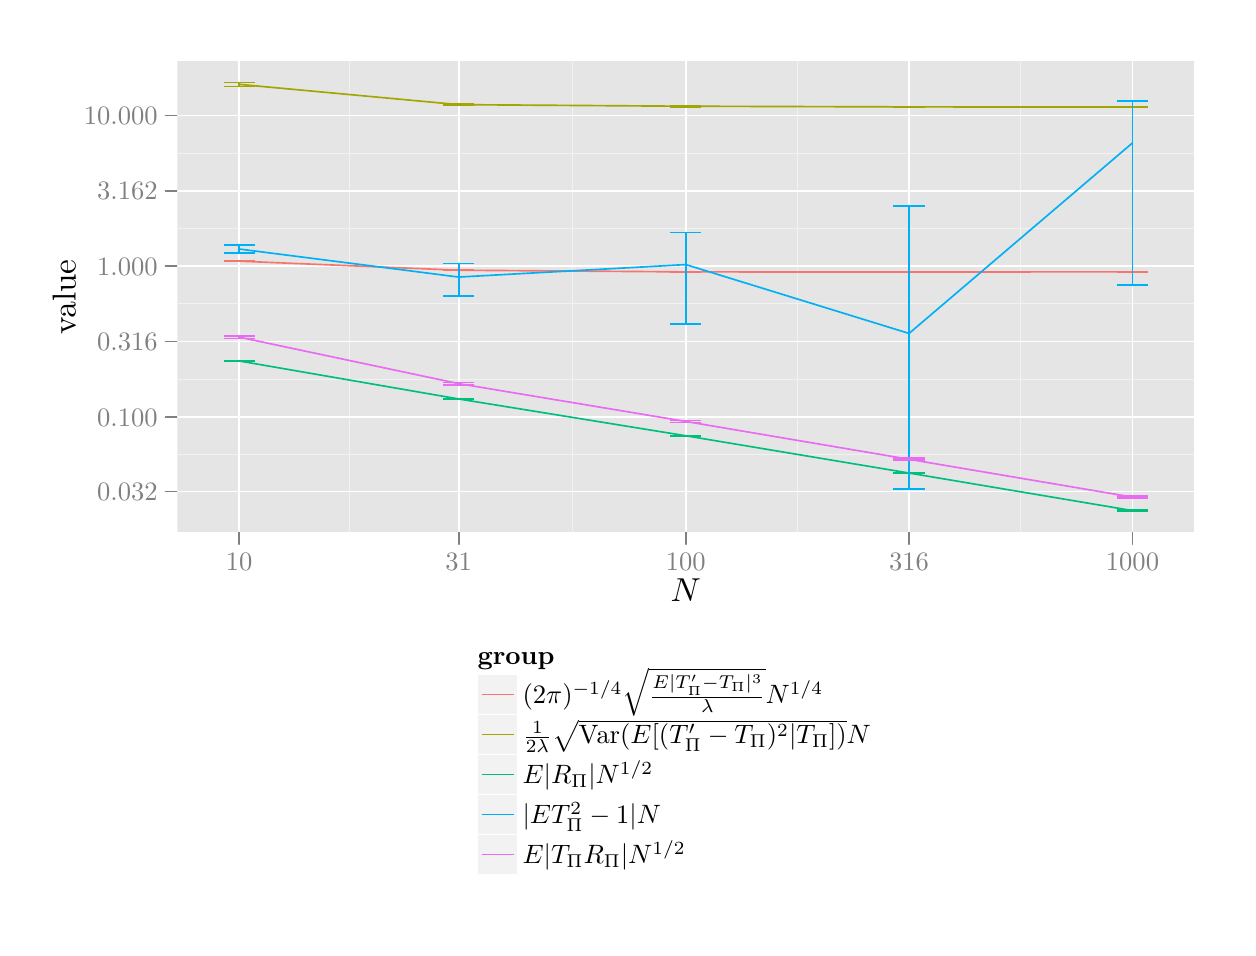
\begin{tikzpicture}[x=1pt,y=1pt]
\definecolor[named]{drawColor}{rgb}{0.00,0.00,0.00}
\definecolor[named]{fillColor}{rgb}{1.00,1.00,1.00}
\fill[color=fillColor,fill opacity=0.00,] (0,0) rectangle (433.62,325.21);
\begin{scope}
\path[clip] (  0.00,  0.00) rectangle (433.62,325.21);
\definecolor[named]{drawColor}{rgb}{0.41,0.16,0.58}
\end{scope}
\begin{scope}
\path[clip] (  0.00,  0.00) rectangle (433.62,325.21);
\definecolor[named]{drawColor}{rgb}{0.41,0.16,0.58}
\end{scope}
\begin{scope}
\path[clip] (  0.00,  0.00) rectangle (433.62,325.21);
\definecolor[named]{drawColor}{rgb}{0.41,0.16,0.58}
\end{scope}
\begin{scope}
\path[clip] (  0.00,  0.00) rectangle (433.62,325.21);
\definecolor[named]{drawColor}{rgb}{0.41,0.16,0.58}
\end{scope}
\begin{scope}
\path[clip] (  0.00,  0.00) rectangle (433.62,325.21);
\definecolor[named]{drawColor}{rgb}{0.41,0.16,0.58}
\end{scope}
\begin{scope}
\path[clip] (  0.00,  0.00) rectangle (433.62,325.21);
\definecolor[named]{drawColor}{rgb}{0.41,0.16,0.58}
\end{scope}
\begin{scope}
\path[clip] (  0.00,  0.00) rectangle (433.62,325.21);
\definecolor[named]{drawColor}{rgb}{0.41,0.16,0.58}
\end{scope}
\begin{scope}
\path[clip] (  0.00,  0.00) rectangle (433.62,325.21);
\definecolor[named]{drawColor}{rgb}{0.41,0.16,0.58}
\end{scope}
\begin{scope}
\path[clip] (  0.00,  0.00) rectangle (433.62,325.21);
\definecolor[named]{drawColor}{rgb}{0.41,0.16,0.58}
\end{scope}
\begin{scope}
\path[clip] (  0.00,  0.00) rectangle (433.62,325.21);
\definecolor[named]{drawColor}{rgb}{0.41,0.16,0.58}
\end{scope}
\begin{scope}
\path[clip] (  0.00,  0.00) rectangle (433.62,325.21);
\definecolor[named]{drawColor}{rgb}{0.41,0.16,0.58}
\end{scope}
\begin{scope}
\path[clip] (  0.00,  0.00) rectangle (433.62,325.21);
\definecolor[named]{drawColor}{rgb}{0.41,0.16,0.58}
\end{scope}
\begin{scope}
\path[clip] ( 54.08,142.81) rectangle (421.57,313.17);
\definecolor[named]{drawColor}{rgb}{0.41,0.16,0.58}
\end{scope}
\begin{scope}
\path[clip] (  0.00,  0.00) rectangle (433.62,325.21);
\definecolor[named]{drawColor}{rgb}{0.41,0.16,0.58}
\end{scope}
\begin{scope}
\path[clip] (  0.00,  0.00) rectangle (433.62,325.21);
\definecolor[named]{drawColor}{rgb}{0.41,0.16,0.58}
\end{scope}
\begin{scope}
\path[clip] (  0.00,  0.00) rectangle (433.62,325.21);
\definecolor[named]{drawColor}{rgb}{0.41,0.16,0.58}
\end{scope}
\begin{scope}
\path[clip] (  0.00,  0.00) rectangle (433.62,325.21);
\definecolor[named]{drawColor}{rgb}{0.41,0.16,0.58}
\end{scope}
\begin{scope}
\path[clip] (  0.00,  0.00) rectangle (433.62,325.21);
\definecolor[named]{drawColor}{rgb}{0.41,0.16,0.58}
\end{scope}
\begin{scope}
\path[clip] (  0.00,  0.00) rectangle (433.62,325.21);
\definecolor[named]{drawColor}{rgb}{0.41,0.16,0.58}
\end{scope}
\begin{scope}
\path[clip] (  0.00,  0.00) rectangle (433.62,325.21);
\definecolor[named]{drawColor}{rgb}{0.41,0.16,0.58}
\end{scope}
\begin{scope}
\path[clip] (  0.00,  0.00) rectangle (433.62,325.21);
\definecolor[named]{drawColor}{rgb}{0.41,0.16,0.58}
\end{scope}
\begin{scope}
\path[clip] (  0.00,  0.00) rectangle (433.62,325.21);
\definecolor[named]{drawColor}{rgb}{0.41,0.16,0.58}
\end{scope}
\begin{scope}
\path[clip] (  0.00,  0.00) rectangle (433.62,325.21);
\definecolor[named]{drawColor}{rgb}{0.41,0.16,0.58}
\end{scope}
\begin{scope}
\path[clip] (  0.00,  0.00) rectangle (433.62,325.21);
\definecolor[named]{drawColor}{rgb}{0.41,0.16,0.58}
\end{scope}
\begin{scope}
\path[clip] (  0.00,  0.00) rectangle (433.62,325.21);
\definecolor[named]{drawColor}{rgb}{0.41,0.16,0.58}
\definecolor[named]{fillColor}{rgb}{1.00,1.00,1.00}

\draw[fill=fillColor,draw opacity=0.00,] (  0.00,  0.00) rectangle (433.62,325.21);
\end{scope}
\begin{scope}
\path[clip] (  0.00,  0.00) rectangle (433.62,325.21);
\definecolor[named]{drawColor}{rgb}{0.41,0.16,0.58}
\end{scope}
\begin{scope}
\path[clip] (  0.00,  0.00) rectangle (433.62,325.21);
\definecolor[named]{drawColor}{rgb}{0.41,0.16,0.58}
\definecolor[named]{drawColor}{rgb}{0.50,0.50,0.50}

\node[color=drawColor,anchor=base east,inner sep=0pt, outer sep=0pt, scale=  0.96] at ( 46.97,154.31) {0.032};

\node[color=drawColor,anchor=base east,inner sep=0pt, outer sep=0pt, scale=  0.96] at ( 46.97,181.26) {0.100};

\node[color=drawColor,anchor=base east,inner sep=0pt, outer sep=0pt, scale=  0.96] at ( 46.97,208.47) {0.316};

\node[color=drawColor,anchor=base east,inner sep=0pt, outer sep=0pt, scale=  0.96] at ( 46.97,235.72) {1.000};

\node[color=drawColor,anchor=base east,inner sep=0pt, outer sep=0pt, scale=  0.96] at ( 46.97,262.94) {3.162};

\node[color=drawColor,anchor=base east,inner sep=0pt, outer sep=0pt, scale=  0.96] at ( 46.97,290.17) {10.000};
\end{scope}
\begin{scope}
\path[clip] (  0.00,  0.00) rectangle (433.62,325.21);
\definecolor[named]{drawColor}{rgb}{0.41,0.16,0.58}
\definecolor[named]{drawColor}{rgb}{0.50,0.50,0.50}

\draw[color=drawColor,line width= 0.6pt,line cap=round,line join=round,fill opacity=0.00,] ( 49.82,157.62) -- ( 54.08,157.62);

\draw[color=drawColor,line width= 0.6pt,line cap=round,line join=round,fill opacity=0.00,] ( 49.82,184.56) -- ( 54.08,184.56);

\draw[color=drawColor,line width= 0.6pt,line cap=round,line join=round,fill opacity=0.00,] ( 49.82,211.78) -- ( 54.08,211.78);

\draw[color=drawColor,line width= 0.6pt,line cap=round,line join=round,fill opacity=0.00,] ( 49.82,239.02) -- ( 54.08,239.02);

\draw[color=drawColor,line width= 0.6pt,line cap=round,line join=round,fill opacity=0.00,] ( 49.82,266.25) -- ( 54.08,266.25);

\draw[color=drawColor,line width= 0.6pt,line cap=round,line join=round,fill opacity=0.00,] ( 49.82,293.48) -- ( 54.08,293.48);
\end{scope}
\begin{scope}
\path[clip] (  0.00,  0.00) rectangle (433.62,325.21);
\definecolor[named]{drawColor}{rgb}{0.41,0.16,0.58}
\end{scope}
\begin{scope}
\path[clip] (  0.00,  0.00) rectangle (433.62,325.21);
\definecolor[named]{drawColor}{rgb}{0.41,0.16,0.58}
\end{scope}
\begin{scope}
\path[clip] (  0.00,  0.00) rectangle (433.62,325.21);
\definecolor[named]{drawColor}{rgb}{0.41,0.16,0.58}
\end{scope}
\begin{scope}
\path[clip] (  0.00,  0.00) rectangle (433.62,325.21);
\definecolor[named]{drawColor}{rgb}{0.41,0.16,0.58}
\end{scope}
\begin{scope}
\path[clip] (  0.00,  0.00) rectangle (433.62,325.21);
\definecolor[named]{drawColor}{rgb}{0.41,0.16,0.58}
\end{scope}
\begin{scope}
\path[clip] ( 54.08,142.81) rectangle (421.57,313.17);
\definecolor[named]{drawColor}{rgb}{0.41,0.16,0.58}
\definecolor[named]{fillColor}{rgb}{0.90,0.90,0.90}

\draw[fill=fillColor,draw opacity=0.00,] ( 54.08,142.81) rectangle (421.57,313.17);
\definecolor[named]{drawColor}{rgb}{0.95,0.95,0.95}

\draw[color=drawColor,line width= 0.3pt,line cap=round,line join=round,fill opacity=0.00,] ( 54.08,171.09) --
	(421.57,171.09);

\draw[color=drawColor,line width= 0.3pt,line cap=round,line join=round,fill opacity=0.00,] ( 54.08,198.17) --
	(421.57,198.17);

\draw[color=drawColor,line width= 0.3pt,line cap=round,line join=round,fill opacity=0.00,] ( 54.08,225.40) --
	(421.57,225.40);

\draw[color=drawColor,line width= 0.3pt,line cap=round,line join=round,fill opacity=0.00,] ( 54.08,252.64) --
	(421.57,252.64);

\draw[color=drawColor,line width= 0.3pt,line cap=round,line join=round,fill opacity=0.00,] ( 54.08,279.87) --
	(421.57,279.87);

\draw[color=drawColor,line width= 0.3pt,line cap=round,line join=round,fill opacity=0.00,] (116.09,142.81) --
	(116.09,313.17);

\draw[color=drawColor,line width= 0.3pt,line cap=round,line join=round,fill opacity=0.00,] (196.78,142.81) --
	(196.78,313.17);

\draw[color=drawColor,line width= 0.3pt,line cap=round,line join=round,fill opacity=0.00,] (278.15,142.81) --
	(278.15,313.17);

\draw[color=drawColor,line width= 0.3pt,line cap=round,line join=round,fill opacity=0.00,] (358.85,142.81) --
	(358.85,313.17);
\definecolor[named]{drawColor}{rgb}{1.00,1.00,1.00}

\draw[color=drawColor,line width= 0.6pt,line cap=round,line join=round,fill opacity=0.00,] ( 54.08,157.62) --
	(421.57,157.62);

\draw[color=drawColor,line width= 0.6pt,line cap=round,line join=round,fill opacity=0.00,] ( 54.08,184.56) --
	(421.57,184.56);

\draw[color=drawColor,line width= 0.6pt,line cap=round,line join=round,fill opacity=0.00,] ( 54.08,211.78) --
	(421.57,211.78);

\draw[color=drawColor,line width= 0.6pt,line cap=round,line join=round,fill opacity=0.00,] ( 54.08,239.02) --
	(421.57,239.02);

\draw[color=drawColor,line width= 0.6pt,line cap=round,line join=round,fill opacity=0.00,] ( 54.08,266.25) --
	(421.57,266.25);

\draw[color=drawColor,line width= 0.6pt,line cap=round,line join=round,fill opacity=0.00,] ( 54.08,293.48) --
	(421.57,293.48);

\draw[color=drawColor,line width= 0.6pt,line cap=round,line join=round,fill opacity=0.00,] ( 76.44,142.81) --
	( 76.44,313.17);

\draw[color=drawColor,line width= 0.6pt,line cap=round,line join=round,fill opacity=0.00,] (155.74,142.81) --
	(155.74,313.17);

\draw[color=drawColor,line width= 0.6pt,line cap=round,line join=round,fill opacity=0.00,] (237.83,142.81) --
	(237.83,313.17);

\draw[color=drawColor,line width= 0.6pt,line cap=round,line join=round,fill opacity=0.00,] (318.48,142.81) --
	(318.48,313.17);

\draw[color=drawColor,line width= 0.6pt,line cap=round,line join=round,fill opacity=0.00,] (399.22,142.81) --
	(399.22,313.17);
\definecolor[named]{drawColor}{rgb}{0.97,0.46,0.43}

\draw[color=drawColor,line width= 0.6pt,line join=round,fill opacity=0.00,] ( 76.44,240.84) --
	(155.74,237.56) --
	(237.83,236.96) --
	(318.48,236.91) --
	(399.22,236.98);
\definecolor[named]{drawColor}{rgb}{0.64,0.65,0.00}

\draw[color=drawColor,line width= 0.6pt,line join=round,fill opacity=0.00,] ( 76.44,304.72) --
	(155.74,297.39) --
	(237.83,296.82) --
	(318.48,296.58) --
	(399.22,296.53);
\definecolor[named]{drawColor}{rgb}{0.00,0.75,0.49}

\draw[color=drawColor,line width= 0.6pt,line join=round,fill opacity=0.00,] ( 76.44,204.77) --
	(155.74,191.04) --
	(237.83,177.74) --
	(318.48,164.27) --
	(399.22,150.70);
\definecolor[named]{drawColor}{rgb}{0.00,0.69,0.96}

\draw[color=drawColor,line width= 0.6pt,line join=round,fill opacity=0.00,] ( 76.44,245.22) --
	(155.74,235.09) --
	(237.83,239.60) --
	(318.48,214.72) --
	(399.22,283.56);
\definecolor[named]{drawColor}{rgb}{0.91,0.42,0.95}

\draw[color=drawColor,line width= 0.6pt,line join=round,fill opacity=0.00,] ( 76.44,213.38) --
	(155.74,196.58) --
	(237.83,182.91) --
	(318.48,169.24) --
	(399.22,155.57);
\definecolor[named]{drawColor}{rgb}{0.97,0.46,0.43}

\draw[color=drawColor,line width= 0.6pt,line join=round,fill opacity=0.00,] ( 70.79,240.89) --
	( 82.08,240.89);

\draw[color=drawColor,line width= 0.6pt,line join=round,fill opacity=0.00,] ( 76.44,240.89) --
	( 76.44,240.78);

\draw[color=drawColor,line width= 0.6pt,line join=round,fill opacity=0.00,] ( 70.79,240.78) --
	( 82.08,240.78);

\draw[color=drawColor,line width= 0.6pt,line join=round,fill opacity=0.00,] (150.09,237.57) --
	(161.39,237.57);

\draw[color=drawColor,line width= 0.6pt,line join=round,fill opacity=0.00,] (155.74,237.57) --
	(155.74,237.56);

\draw[color=drawColor,line width= 0.6pt,line join=round,fill opacity=0.00,] (150.09,237.56) --
	(161.39,237.56);

\draw[color=drawColor,line width= 0.6pt,line join=round,fill opacity=0.00,] (232.18,236.96) --
	(243.48,236.96);

\draw[color=drawColor,line width= 0.6pt,line join=round,fill opacity=0.00,] (237.83,236.96) --
	(237.83,236.96);

\draw[color=drawColor,line width= 0.6pt,line join=round,fill opacity=0.00,] (232.18,236.96) --
	(243.48,236.96);

\draw[color=drawColor,line width= 0.6pt,line join=round,fill opacity=0.00,] (312.83,236.91) --
	(324.12,236.91);

\draw[color=drawColor,line width= 0.6pt,line join=round,fill opacity=0.00,] (318.48,236.91) --
	(318.48,236.91);

\draw[color=drawColor,line width= 0.6pt,line join=round,fill opacity=0.00,] (312.83,236.91) --
	(324.12,236.91);

\draw[color=drawColor,line width= 0.6pt,line join=round,fill opacity=0.00,] (393.57,236.98) --
	(404.87,236.98);

\draw[color=drawColor,line width= 0.6pt,line join=round,fill opacity=0.00,] (399.22,236.98) --
	(399.22,236.98);

\draw[color=drawColor,line width= 0.6pt,line join=round,fill opacity=0.00,] (393.57,236.98) --
	(404.87,236.98);
\definecolor[named]{drawColor}{rgb}{0.64,0.65,0.00}

\draw[color=drawColor,line width= 0.6pt,line join=round,fill opacity=0.00,] ( 70.79,305.43) --
	( 82.08,305.43);

\draw[color=drawColor,line width= 0.6pt,line join=round,fill opacity=0.00,] ( 76.44,305.43) --
	( 76.44,304.01);

\draw[color=drawColor,line width= 0.6pt,line join=round,fill opacity=0.00,] ( 70.79,304.01) --
	( 82.08,304.01);

\draw[color=drawColor,line width= 0.6pt,line join=round,fill opacity=0.00,] (150.09,297.68) --
	(161.39,297.68);

\draw[color=drawColor,line width= 0.6pt,line join=round,fill opacity=0.00,] (155.74,297.68) --
	(155.74,297.13);

\draw[color=drawColor,line width= 0.6pt,line join=round,fill opacity=0.00,] (150.09,297.13) --
	(161.39,297.13);

\draw[color=drawColor,line width= 0.6pt,line join=round,fill opacity=0.00,] (232.18,297.05) --
	(243.48,297.05);

\draw[color=drawColor,line width= 0.6pt,line join=round,fill opacity=0.00,] (237.83,297.05) --
	(237.83,296.59);

\draw[color=drawColor,line width= 0.6pt,line join=round,fill opacity=0.00,] (232.18,296.59) --
	(243.48,296.59);

\draw[color=drawColor,line width= 0.6pt,line join=round,fill opacity=0.00,] (312.83,296.77) --
	(324.12,296.77);

\draw[color=drawColor,line width= 0.6pt,line join=round,fill opacity=0.00,] (318.48,296.77) --
	(318.48,296.39);

\draw[color=drawColor,line width= 0.6pt,line join=round,fill opacity=0.00,] (312.83,296.39) --
	(324.12,296.39);

\draw[color=drawColor,line width= 0.6pt,line join=round,fill opacity=0.00,] (393.57,296.72) --
	(404.87,296.72);

\draw[color=drawColor,line width= 0.6pt,line join=round,fill opacity=0.00,] (399.22,296.72) --
	(399.22,296.35);

\draw[color=drawColor,line width= 0.6pt,line join=round,fill opacity=0.00,] (393.57,296.35) --
	(404.87,296.35);
\definecolor[named]{drawColor}{rgb}{0.00,0.75,0.49}

\draw[color=drawColor,line width= 0.6pt,line join=round,fill opacity=0.00,] ( 70.79,204.94) --
	( 82.08,204.94);

\draw[color=drawColor,line width= 0.6pt,line join=round,fill opacity=0.00,] ( 76.44,204.94) --
	( 76.44,204.60);

\draw[color=drawColor,line width= 0.6pt,line join=round,fill opacity=0.00,] ( 70.79,204.60) --
	( 82.08,204.60);

\draw[color=drawColor,line width= 0.6pt,line join=round,fill opacity=0.00,] (150.09,191.19) --
	(161.39,191.19);

\draw[color=drawColor,line width= 0.6pt,line join=round,fill opacity=0.00,] (155.74,191.19) --
	(155.74,190.91);

\draw[color=drawColor,line width= 0.6pt,line join=round,fill opacity=0.00,] (150.09,190.91) --
	(161.39,190.91);

\draw[color=drawColor,line width= 0.6pt,line join=round,fill opacity=0.00,] (232.18,177.87) --
	(243.48,177.87);

\draw[color=drawColor,line width= 0.6pt,line join=round,fill opacity=0.00,] (237.83,177.87) --
	(237.83,177.59);

\draw[color=drawColor,line width= 0.6pt,line join=round,fill opacity=0.00,] (232.18,177.59) --
	(243.48,177.59);

\draw[color=drawColor,line width= 0.6pt,line join=round,fill opacity=0.00,] (312.83,164.39) --
	(324.12,164.39);

\draw[color=drawColor,line width= 0.6pt,line join=round,fill opacity=0.00,] (318.48,164.39) --
	(318.48,164.14);

\draw[color=drawColor,line width= 0.6pt,line join=round,fill opacity=0.00,] (312.83,164.14) --
	(324.12,164.14);

\draw[color=drawColor,line width= 0.6pt,line join=round,fill opacity=0.00,] (393.57,150.82) --
	(404.87,150.82);

\draw[color=drawColor,line width= 0.6pt,line join=round,fill opacity=0.00,] (399.22,150.82) --
	(399.22,150.56);

\draw[color=drawColor,line width= 0.6pt,line join=round,fill opacity=0.00,] (393.57,150.56) --
	(404.87,150.56);
\definecolor[named]{drawColor}{rgb}{0.00,0.69,0.96}

\draw[color=drawColor,line width= 0.6pt,line join=round,fill opacity=0.00,] ( 70.79,246.60) --
	( 82.08,246.60);

\draw[color=drawColor,line width= 0.6pt,line join=round,fill opacity=0.00,] ( 76.44,246.60) --
	( 76.44,243.72);

\draw[color=drawColor,line width= 0.6pt,line join=round,fill opacity=0.00,] ( 70.79,243.72) --
	( 82.08,243.72);

\draw[color=drawColor,line width= 0.6pt,line join=round,fill opacity=0.00,] (150.09,239.93) --
	(161.39,239.93);

\draw[color=drawColor,line width= 0.6pt,line join=round,fill opacity=0.00,] (155.74,239.93) --
	(155.74,228.31);

\draw[color=drawColor,line width= 0.6pt,line join=round,fill opacity=0.00,] (150.09,228.31) --
	(161.39,228.31);

\draw[color=drawColor,line width= 0.6pt,line join=round,fill opacity=0.00,] (232.18,251.16) --
	(243.48,251.16);

\draw[color=drawColor,line width= 0.6pt,line join=round,fill opacity=0.00,] (237.83,251.16) --
	(237.83,218.23);

\draw[color=drawColor,line width= 0.6pt,line join=round,fill opacity=0.00,] (232.18,218.23) --
	(243.48,218.23);

\draw[color=drawColor,line width= 0.6pt,line join=round,fill opacity=0.00,] (312.83,260.65) --
	(324.12,260.65);

\draw[color=drawColor,line width= 0.6pt,line join=round,fill opacity=0.00,] (318.48,260.65) --
	(318.48,158.40);

\draw[color=drawColor,line width= 0.6pt,line join=round,fill opacity=0.00,] (312.83,158.40) --
	(324.12,158.40);

\draw[color=drawColor,line width= 0.6pt,line join=round,fill opacity=0.00,] (393.57,298.71) --
	(404.87,298.71);

\draw[color=drawColor,line width= 0.6pt,line join=round,fill opacity=0.00,] (399.22,298.71) --
	(399.22,232.33);

\draw[color=drawColor,line width= 0.6pt,line join=round,fill opacity=0.00,] (393.57,232.33) --
	(404.87,232.33);
\definecolor[named]{drawColor}{rgb}{0.91,0.42,0.95}

\draw[color=drawColor,line width= 0.6pt,line join=round,fill opacity=0.00,] ( 70.79,213.89) --
	( 82.08,213.89);

\draw[color=drawColor,line width= 0.6pt,line join=round,fill opacity=0.00,] ( 76.44,213.89) --
	( 76.44,212.86);

\draw[color=drawColor,line width= 0.6pt,line join=round,fill opacity=0.00,] ( 70.79,212.86) --
	( 82.08,212.86);

\draw[color=drawColor,line width= 0.6pt,line join=round,fill opacity=0.00,] (150.09,196.96) --
	(161.39,196.96);

\draw[color=drawColor,line width= 0.6pt,line join=round,fill opacity=0.00,] (155.74,196.96) --
	(155.74,196.20);

\draw[color=drawColor,line width= 0.6pt,line join=round,fill opacity=0.00,] (150.09,196.20) --
	(161.39,196.20);

\draw[color=drawColor,line width= 0.6pt,line join=round,fill opacity=0.00,] (232.18,183.31) --
	(243.48,183.31);

\draw[color=drawColor,line width= 0.6pt,line join=round,fill opacity=0.00,] (237.83,183.31) --
	(237.83,182.54);

\draw[color=drawColor,line width= 0.6pt,line join=round,fill opacity=0.00,] (232.18,182.54) --
	(243.48,182.54);

\draw[color=drawColor,line width= 0.6pt,line join=round,fill opacity=0.00,] (312.83,169.60) --
	(324.12,169.60);

\draw[color=drawColor,line width= 0.6pt,line join=round,fill opacity=0.00,] (318.48,169.60) --
	(318.48,168.89);

\draw[color=drawColor,line width= 0.6pt,line join=round,fill opacity=0.00,] (312.83,168.89) --
	(324.12,168.89);

\draw[color=drawColor,line width= 0.6pt,line join=round,fill opacity=0.00,] (393.57,155.90) --
	(404.87,155.90);

\draw[color=drawColor,line width= 0.6pt,line join=round,fill opacity=0.00,] (399.22,155.90) --
	(399.22,155.26);

\draw[color=drawColor,line width= 0.6pt,line join=round,fill opacity=0.00,] (393.57,155.26) --
	(404.87,155.26);
\end{scope}
\begin{scope}
\path[clip] (  0.00,  0.00) rectangle (433.62,325.21);
\definecolor[named]{drawColor}{rgb}{0.41,0.16,0.58}
\end{scope}
\begin{scope}
\path[clip] (  0.00,  0.00) rectangle (433.62,325.21);
\definecolor[named]{drawColor}{rgb}{0.41,0.16,0.58}
\definecolor[named]{drawColor}{rgb}{0.50,0.50,0.50}

\node[color=drawColor,anchor=base,inner sep=0pt, outer sep=0pt, scale=  0.96] at ( 76.44,129.09) {10};

\node[color=drawColor,anchor=base,inner sep=0pt, outer sep=0pt, scale=  0.96] at (155.74,129.09) {31};

\node[color=drawColor,anchor=base,inner sep=0pt, outer sep=0pt, scale=  0.96] at (237.83,129.09) {100};

\node[color=drawColor,anchor=base,inner sep=0pt, outer sep=0pt, scale=  0.96] at (318.48,129.09) {316};

\node[color=drawColor,anchor=base,inner sep=0pt, outer sep=0pt, scale=  0.96] at (399.22,129.09) {1000};
\end{scope}
\begin{scope}
\path[clip] (  0.00,  0.00) rectangle (433.62,325.21);
\definecolor[named]{drawColor}{rgb}{0.41,0.16,0.58}
\definecolor[named]{drawColor}{rgb}{0.50,0.50,0.50}

\draw[color=drawColor,line width= 0.6pt,line cap=round,line join=round,fill opacity=0.00,] ( 76.44,138.55) -- ( 76.44,142.81);

\draw[color=drawColor,line width= 0.6pt,line cap=round,line join=round,fill opacity=0.00,] (155.74,138.55) -- (155.74,142.81);

\draw[color=drawColor,line width= 0.6pt,line cap=round,line join=round,fill opacity=0.00,] (237.83,138.55) -- (237.83,142.81);

\draw[color=drawColor,line width= 0.6pt,line cap=round,line join=round,fill opacity=0.00,] (318.48,138.55) -- (318.48,142.81);

\draw[color=drawColor,line width= 0.6pt,line cap=round,line join=round,fill opacity=0.00,] (399.22,138.55) -- (399.22,142.81);
\end{scope}
\begin{scope}
\path[clip] (  0.00,  0.00) rectangle (433.62,325.21);
\definecolor[named]{drawColor}{rgb}{0.41,0.16,0.58}
\end{scope}
\begin{scope}
\path[clip] (  0.00,  0.00) rectangle (433.62,325.21);
\definecolor[named]{drawColor}{rgb}{0.41,0.16,0.58}
\end{scope}
\begin{scope}
\path[clip] (  0.00,  0.00) rectangle (433.62,325.21);
\definecolor[named]{drawColor}{rgb}{0.41,0.16,0.58}
\end{scope}
\begin{scope}
\path[clip] (  0.00,  0.00) rectangle (433.62,325.21);
\definecolor[named]{drawColor}{rgb}{0.41,0.16,0.58}
\end{scope}
\begin{scope}
\path[clip] (  0.00,  0.00) rectangle (433.62,325.21);
\definecolor[named]{drawColor}{rgb}{0.41,0.16,0.58}
\end{scope}
\begin{scope}
\path[clip] (  0.00,  0.00) rectangle (433.62,325.21);
\definecolor[named]{drawColor}{rgb}{0.41,0.16,0.58}
\definecolor[named]{drawColor}{rgb}{0.00,0.00,0.00}

\node[color=drawColor,anchor=base,inner sep=0pt, outer sep=0pt, scale=  1.20] at (237.83,117.81) {$N$};
\end{scope}
\begin{scope}
\path[clip] (  0.00,  0.00) rectangle (433.62,325.21);
\definecolor[named]{drawColor}{rgb}{0.41,0.16,0.58}
\end{scope}
\begin{scope}
\path[clip] (  0.00,  0.00) rectangle (433.62,325.21);
\definecolor[named]{drawColor}{rgb}{0.41,0.16,0.58}
\definecolor[named]{drawColor}{rgb}{0.00,0.00,0.00}

\node[rotate= 90.00,color=drawColor,anchor=base,inner sep=0pt, outer sep=0pt, scale=  1.20] at ( 17.30,227.99) {value};
\end{scope}
\begin{scope}
\path[clip] (  0.00,  0.00) rectangle (433.62,325.21);
\definecolor[named]{drawColor}{rgb}{0.41,0.16,0.58}
\end{scope}
\begin{scope}
\path[clip] (  0.00,  0.00) rectangle (433.62,325.21);
\definecolor[named]{drawColor}{rgb}{0.41,0.16,0.58}
\end{scope}
\begin{scope}
\path[clip] (  0.00,  0.00) rectangle (433.62,325.21);
\definecolor[named]{drawColor}{rgb}{0.41,0.16,0.58}
\end{scope}
\begin{scope}
\path[clip] (  0.00,  0.00) rectangle (433.62,325.21);
\definecolor[named]{drawColor}{rgb}{0.41,0.16,0.58}
\end{scope}
\begin{scope}
\path[clip] (  0.00,  0.00) rectangle (433.62,325.21);
\definecolor[named]{drawColor}{rgb}{0.41,0.16,0.58}
\end{scope}
\begin{scope}
\path[clip] (  0.00,  0.00) rectangle (433.62,325.21);
\definecolor[named]{drawColor}{rgb}{0.41,0.16,0.58}
\end{scope}
\begin{scope}
\path[clip] (  0.00,  0.00) rectangle (433.62,325.21);
\definecolor[named]{drawColor}{rgb}{0.41,0.16,0.58}
\end{scope}
\begin{scope}
\path[clip] (  0.00,  0.00) rectangle (433.62,325.21);
\definecolor[named]{drawColor}{rgb}{0.41,0.16,0.58}
\end{scope}
\begin{scope}
\path[clip] (  0.00,  0.00) rectangle (433.62,325.21);
\definecolor[named]{drawColor}{rgb}{0.41,0.16,0.58}
\end{scope}
\begin{scope}
\path[clip] (  0.00,  0.00) rectangle (433.62,325.21);
\definecolor[named]{drawColor}{rgb}{0.41,0.16,0.58}
\end{scope}
\begin{scope}
\path[clip] (  0.00,  0.00) rectangle (433.62,325.21);
\definecolor[named]{drawColor}{rgb}{0.41,0.16,0.58}
\end{scope}
\begin{scope}
\path[clip] (  0.00,  0.00) rectangle (433.62,325.21);
\definecolor[named]{drawColor}{rgb}{0.41,0.16,0.58}
\end{scope}
\begin{scope}
\path[clip] (  0.00,  0.00) rectangle (433.62,325.21);
\definecolor[named]{drawColor}{rgb}{0.41,0.16,0.58}
\end{scope}
\begin{scope}
\path[clip] (  0.00,  0.00) rectangle (433.62,325.21);
\definecolor[named]{drawColor}{rgb}{0.41,0.16,0.58}
\end{scope}
\begin{scope}
\path[clip] (  0.00,  0.00) rectangle (433.62,325.21);
\definecolor[named]{drawColor}{rgb}{0.41,0.16,0.58}
\end{scope}
\begin{scope}
\path[clip] (  0.00,  0.00) rectangle (433.62,325.21);
\definecolor[named]{drawColor}{rgb}{0.41,0.16,0.58}
\end{scope}
\begin{scope}
\path[clip] (  0.00,  0.00) rectangle (433.62,325.21);
\definecolor[named]{drawColor}{rgb}{0.41,0.16,0.58}
\end{scope}
\begin{scope}
\path[clip] (  0.00,  0.00) rectangle (433.62,325.21);
\definecolor[named]{drawColor}{rgb}{0.41,0.16,0.58}
\end{scope}
\begin{scope}
\path[clip] (  0.00,  0.00) rectangle (433.62,325.21);
\definecolor[named]{drawColor}{rgb}{0.41,0.16,0.58}
\end{scope}
\begin{scope}
\path[clip] (  0.00,  0.00) rectangle (433.62,325.21);
\definecolor[named]{drawColor}{rgb}{0.41,0.16,0.58}
\end{scope}
\begin{scope}
\path[clip] (  0.00,  0.00) rectangle (433.62,325.21);
\definecolor[named]{drawColor}{rgb}{0.41,0.16,0.58}
\end{scope}
\begin{scope}
\path[clip] (  0.00,  0.00) rectangle (433.62,325.21);
\definecolor[named]{drawColor}{rgb}{0.41,0.16,0.58}
\end{scope}
\begin{scope}
\path[clip] (  0.00,  0.00) rectangle (433.62,325.21);
\definecolor[named]{drawColor}{rgb}{0.41,0.16,0.58}
\end{scope}
\begin{scope}
\path[clip] (  0.00,  0.00) rectangle (433.62,325.21);
\definecolor[named]{drawColor}{rgb}{0.41,0.16,0.58}
\end{scope}
\begin{scope}
\path[clip] (  0.00,  0.00) rectangle (433.62,325.21);
\definecolor[named]{drawColor}{rgb}{0.41,0.16,0.58}
\definecolor[named]{drawColor}{rgb}{1.00,1.00,1.00}

\draw[color=drawColor,line width= 0.6pt,line cap=round,line join=round,fill opacity=0.00,] (158.31, 14.89) rectangle (317.35,105.93);
\end{scope}
\begin{scope}
\path[clip] (  0.00,  0.00) rectangle (433.62,325.21);
\definecolor[named]{drawColor}{rgb}{0.41,0.16,0.58}
\definecolor[named]{drawColor}{rgb}{0.00,0.00,0.00}

\node[color=drawColor,anchor=base west,inner sep=0pt, outer sep=0pt, scale=  0.96] at (162.58, 95.04) {\bfseries group};
\end{scope}
\begin{scope}
\path[clip] (  0.00,  0.00) rectangle (433.62,325.21);
\definecolor[named]{drawColor}{rgb}{0.41,0.16,0.58}
\definecolor[named]{drawColor}{rgb}{1.00,1.00,1.00}
\definecolor[named]{fillColor}{rgb}{0.95,0.95,0.95}

\draw[color=drawColor,line width= 0.6pt,line cap=round,line join=round,fill=fillColor,] (162.58, 76.97) rectangle (177.03, 91.43);
\end{scope}
\begin{scope}
\path[clip] (  0.00,  0.00) rectangle (433.62,325.21);
\definecolor[named]{drawColor}{rgb}{0.41,0.16,0.58}
\definecolor[named]{drawColor}{rgb}{0.97,0.46,0.43}

\draw[color=drawColor,line width= 0.6pt,line join=round,fill opacity=0.00,] (164.02, 84.20) -- (175.58, 84.20);
\end{scope}
\begin{scope}
\path[clip] (  0.00,  0.00) rectangle (433.62,325.21);
\definecolor[named]{drawColor}{rgb}{0.41,0.16,0.58}
\definecolor[named]{drawColor}{rgb}{0.97,0.46,0.43}

\draw[color=drawColor,line width= 0.6pt,line join=round,fill opacity=0.00,] (164.02, 84.20) -- (175.58, 84.20);
\end{scope}
\begin{scope}
\path[clip] (  0.00,  0.00) rectangle (433.62,325.21);
\definecolor[named]{drawColor}{rgb}{0.41,0.16,0.58}
\definecolor[named]{drawColor}{rgb}{1.00,1.00,1.00}
\definecolor[named]{fillColor}{rgb}{0.95,0.95,0.95}

\draw[color=drawColor,line width= 0.6pt,line cap=round,line join=round,fill=fillColor,] (162.58, 62.52) rectangle (177.03, 76.97);
\end{scope}
\begin{scope}
\path[clip] (  0.00,  0.00) rectangle (433.62,325.21);
\definecolor[named]{drawColor}{rgb}{0.41,0.16,0.58}
\definecolor[named]{drawColor}{rgb}{0.64,0.65,0.00}

\draw[color=drawColor,line width= 0.6pt,line join=round,fill opacity=0.00,] (164.02, 69.75) -- (175.58, 69.75);
\end{scope}
\begin{scope}
\path[clip] (  0.00,  0.00) rectangle (433.62,325.21);
\definecolor[named]{drawColor}{rgb}{0.41,0.16,0.58}
\definecolor[named]{drawColor}{rgb}{0.64,0.65,0.00}

\draw[color=drawColor,line width= 0.6pt,line join=round,fill opacity=0.00,] (164.02, 69.75) -- (175.58, 69.75);
\end{scope}
\begin{scope}
\path[clip] (  0.00,  0.00) rectangle (433.62,325.21);
\definecolor[named]{drawColor}{rgb}{0.41,0.16,0.58}
\definecolor[named]{drawColor}{rgb}{1.00,1.00,1.00}
\definecolor[named]{fillColor}{rgb}{0.95,0.95,0.95}

\draw[color=drawColor,line width= 0.6pt,line cap=round,line join=round,fill=fillColor,] (162.58, 48.07) rectangle (177.03, 62.52);
\end{scope}
\begin{scope}
\path[clip] (  0.00,  0.00) rectangle (433.62,325.21);
\definecolor[named]{drawColor}{rgb}{0.41,0.16,0.58}
\definecolor[named]{drawColor}{rgb}{0.00,0.75,0.49}

\draw[color=drawColor,line width= 0.6pt,line join=round,fill opacity=0.00,] (164.02, 55.29) -- (175.58, 55.29);
\end{scope}
\begin{scope}
\path[clip] (  0.00,  0.00) rectangle (433.62,325.21);
\definecolor[named]{drawColor}{rgb}{0.41,0.16,0.58}
\definecolor[named]{drawColor}{rgb}{0.00,0.75,0.49}

\draw[color=drawColor,line width= 0.6pt,line join=round,fill opacity=0.00,] (164.02, 55.29) -- (175.58, 55.29);
\end{scope}
\begin{scope}
\path[clip] (  0.00,  0.00) rectangle (433.62,325.21);
\definecolor[named]{drawColor}{rgb}{0.41,0.16,0.58}
\definecolor[named]{drawColor}{rgb}{1.00,1.00,1.00}
\definecolor[named]{fillColor}{rgb}{0.95,0.95,0.95}

\draw[color=drawColor,line width= 0.6pt,line cap=round,line join=round,fill=fillColor,] (162.58, 33.61) rectangle (177.03, 48.07);
\end{scope}
\begin{scope}
\path[clip] (  0.00,  0.00) rectangle (433.62,325.21);
\definecolor[named]{drawColor}{rgb}{0.41,0.16,0.58}
\definecolor[named]{drawColor}{rgb}{0.00,0.69,0.96}

\draw[color=drawColor,line width= 0.6pt,line join=round,fill opacity=0.00,] (164.02, 40.84) -- (175.58, 40.84);
\end{scope}
\begin{scope}
\path[clip] (  0.00,  0.00) rectangle (433.62,325.21);
\definecolor[named]{drawColor}{rgb}{0.41,0.16,0.58}
\definecolor[named]{drawColor}{rgb}{0.00,0.69,0.96}

\draw[color=drawColor,line width= 0.6pt,line join=round,fill opacity=0.00,] (164.02, 40.84) -- (175.58, 40.84);
\end{scope}
\begin{scope}
\path[clip] (  0.00,  0.00) rectangle (433.62,325.21);
\definecolor[named]{drawColor}{rgb}{0.41,0.16,0.58}
\definecolor[named]{drawColor}{rgb}{1.00,1.00,1.00}
\definecolor[named]{fillColor}{rgb}{0.95,0.95,0.95}

\draw[color=drawColor,line width= 0.6pt,line cap=round,line join=round,fill=fillColor,] (162.58, 19.16) rectangle (177.03, 33.61);
\end{scope}
\begin{scope}
\path[clip] (  0.00,  0.00) rectangle (433.62,325.21);
\definecolor[named]{drawColor}{rgb}{0.41,0.16,0.58}
\definecolor[named]{drawColor}{rgb}{0.91,0.42,0.95}

\draw[color=drawColor,line width= 0.6pt,line join=round,fill opacity=0.00,] (164.02, 26.39) -- (175.58, 26.39);
\end{scope}
\begin{scope}
\path[clip] (  0.00,  0.00) rectangle (433.62,325.21);
\definecolor[named]{drawColor}{rgb}{0.41,0.16,0.58}
\definecolor[named]{drawColor}{rgb}{0.91,0.42,0.95}

\draw[color=drawColor,line width= 0.6pt,line join=round,fill opacity=0.00,] (164.02, 26.39) -- (175.58, 26.39);
\end{scope}
\begin{scope}
\path[clip] (  0.00,  0.00) rectangle (433.62,325.21);
\definecolor[named]{drawColor}{rgb}{0.41,0.16,0.58}
\definecolor[named]{drawColor}{rgb}{0.00,0.00,0.00}

\node[color=drawColor,anchor=base west,inner sep=0pt, outer sep=0pt, scale=  0.96] at (178.84, 80.90) {$(2\pi)^{-1/4}\sqrt{\frac{\mathbb{E}|T'_{\Pi}-T_{\Pi}|^3}{\lambda}}N^{1/4}\quad $};
\end{scope}
\begin{scope}
\path[clip] (  0.00,  0.00) rectangle (433.62,325.21);
\definecolor[named]{drawColor}{rgb}{0.41,0.16,0.58}
\definecolor[named]{drawColor}{rgb}{0.00,0.00,0.00}

\node[color=drawColor,anchor=base west,inner sep=0pt, outer sep=0pt, scale=  0.96] at (178.84, 66.44) {$\frac{1}{2\lambda}\sqrt{\mathrm{Var}(\mathbb{E}[(T'_{\Pi}-T_{\Pi})^2|T_{\Pi}])}N\quad $};
\end{scope}
\begin{scope}
\path[clip] (  0.00,  0.00) rectangle (433.62,325.21);
\definecolor[named]{drawColor}{rgb}{0.41,0.16,0.58}
\definecolor[named]{drawColor}{rgb}{0.00,0.00,0.00}

\node[color=drawColor,anchor=base west,inner sep=0pt, outer sep=0pt, scale=  0.96] at (178.84, 51.99) {$\mathbb{E}|R_{\Pi}|N^{1/2}\quad $};
\end{scope}
\begin{scope}
\path[clip] (  0.00,  0.00) rectangle (433.62,325.21);
\definecolor[named]{drawColor}{rgb}{0.41,0.16,0.58}
\definecolor[named]{drawColor}{rgb}{0.00,0.00,0.00}

\node[color=drawColor,anchor=base west,inner sep=0pt, outer sep=0pt, scale=  0.96] at (178.84, 37.53) {$|\mathbb{E}T_{\Pi}^2-1|N\quad $};
\end{scope}
\begin{scope}
\path[clip] (  0.00,  0.00) rectangle (433.62,325.21);
\definecolor[named]{drawColor}{rgb}{0.41,0.16,0.58}
\definecolor[named]{drawColor}{rgb}{0.00,0.00,0.00}

\node[color=drawColor,anchor=base west,inner sep=0pt, outer sep=0pt, scale=  0.96] at (178.84, 23.08) {$\mathbb{E}|T_{\Pi}R_{\Pi}|N^{1/2}\quad $};
\end{scope}
\begin{scope}
\path[clip] (  0.00,  0.00) rectangle (433.62,325.21);
\definecolor[named]{drawColor}{rgb}{0.41,0.16,0.58}
\end{scope}
\begin{scope}
\path[clip] (  0.00,  0.00) rectangle (433.62,325.21);
\definecolor[named]{drawColor}{rgb}{0.41,0.16,0.58}
\end{scope}
\begin{scope}
\path[clip] (  0.00,  0.00) rectangle (433.62,325.21);
\definecolor[named]{drawColor}{rgb}{0.41,0.16,0.58}
\end{scope}
\end{tikzpicture}

  \caption{Log-log plot of values for each term in the bound, calculating the conditional
    expectation exactly (200,000 permutations each).}
\end{figure}

Our bounds appear to be of the correct order or slightly conservative in some cases.  The bounds on
the remainder terms ($\E |R_{\Pi}|$ and $\E |T_{\Pi}R_{\Pi}|$) are of order $N^{1/2}$, but the true
rates are probably lower.
\clearpage

\section{True Rate}
To assess the true rate of convergence, we consider two settings: the earlier Normal setting and
group draws from a Cauchy distribution with location parameters $-1$ and $1$ depending on the
group.  Our bounds include a dependence on $u_{\Delta} = \max_i u_{i} - \min_i u_{i}$.  To better
understand the differences between these two models, we simulate the minimum and maximum scaled
(mean $0$ and sum of squares $2N$) values:
\begin{figure}[!ht]
  \centering
  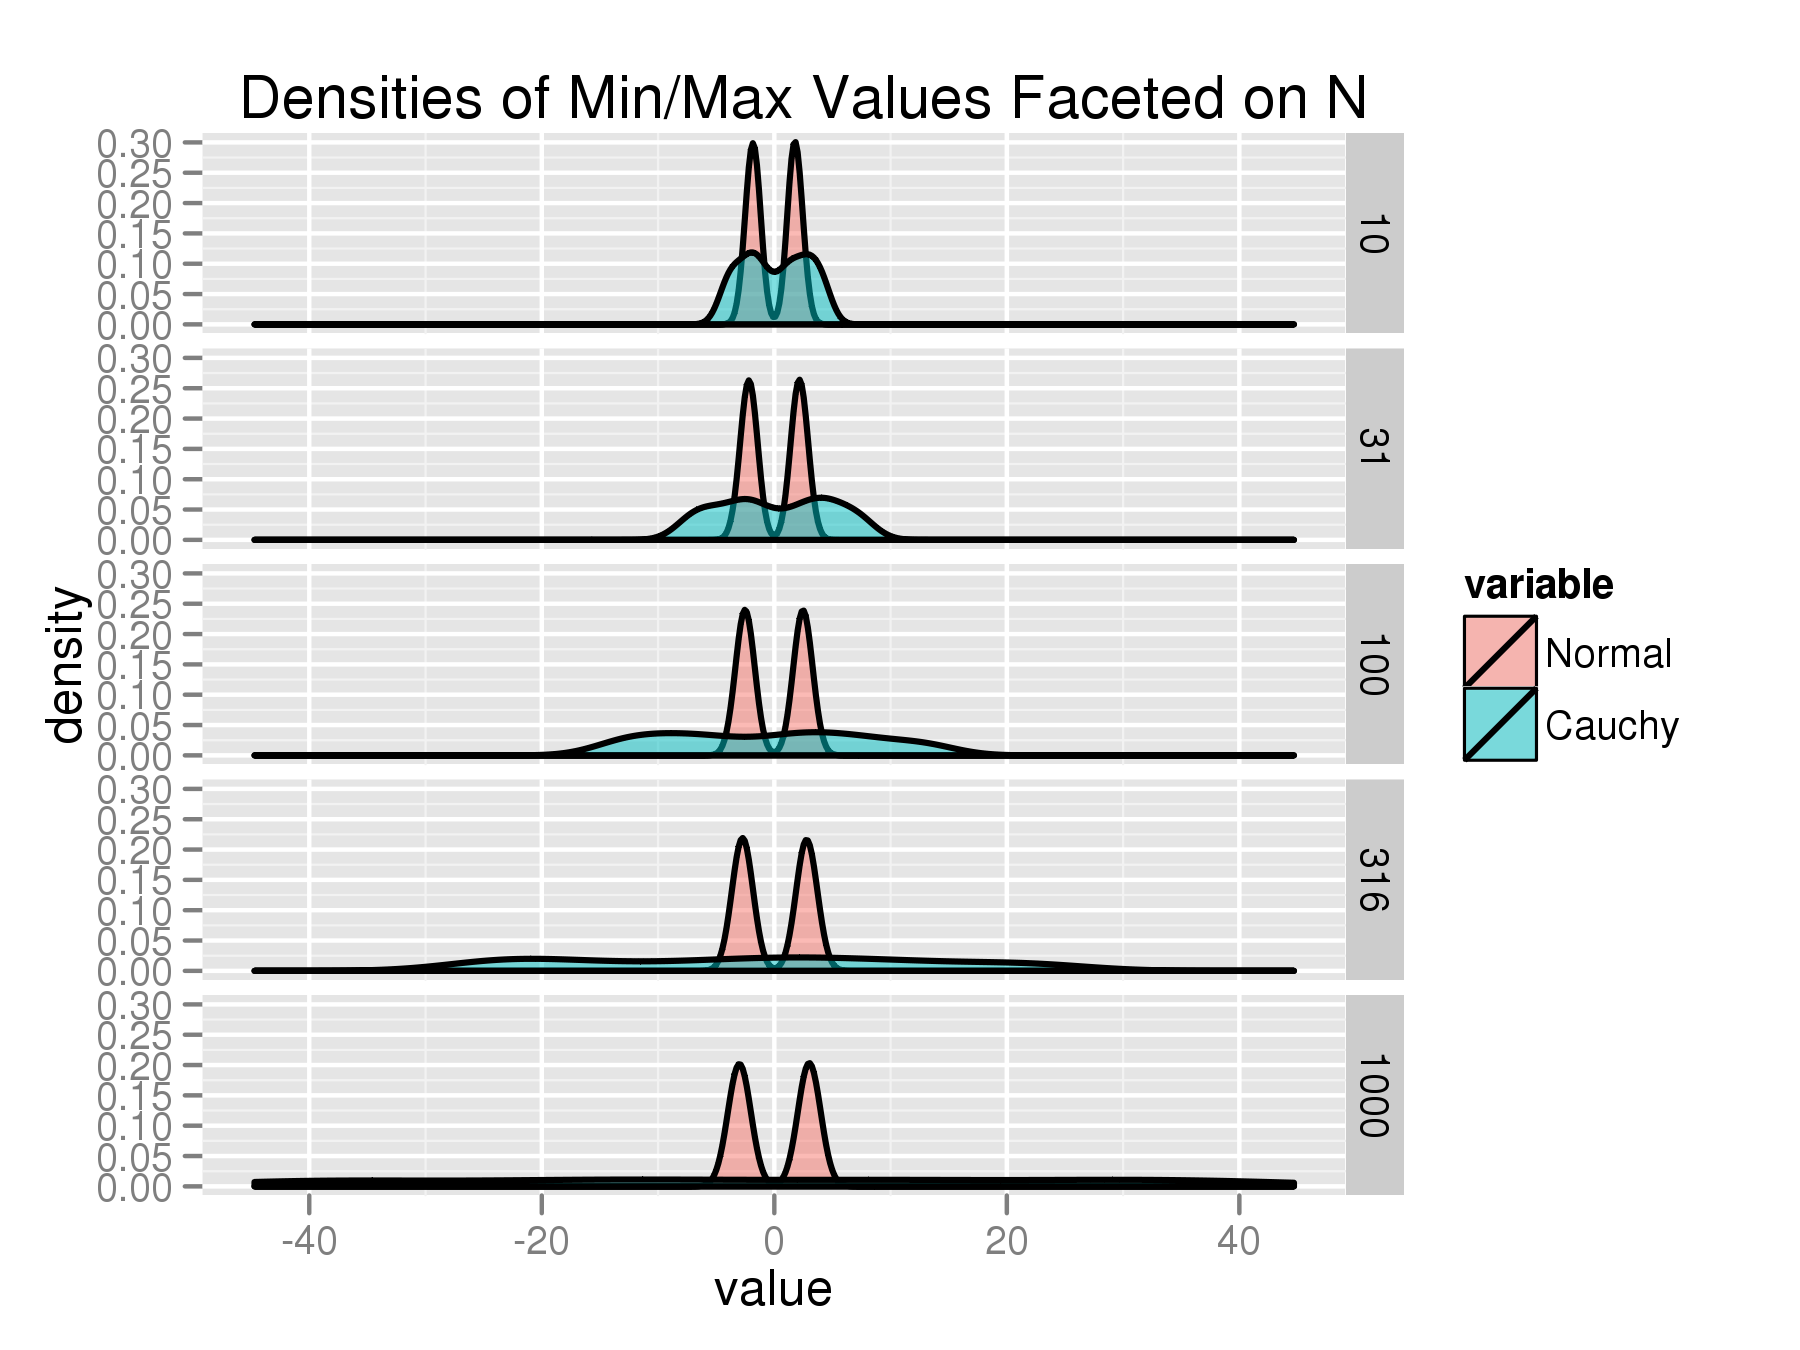
\includegraphics{./simulations/sim5.png}
\end{figure}

For $N=1000$, the Normal model typically has $u_{\Delta}$ values around 6.  In contrast, the Cauchy
model has $u_{\Delta}$ values closer to 40.  
\clearpage

Here, we plot the empirical Kolmogorov-Smirnov test statistic in the following three settings:
\begin{enumerate}
\item a standard Normal draw of size $N$ (repeated N times to get the empirical distribution)
\item the permutation $t$-statistic under Cauchy sampling (N permutations)
\item the permutation $t$-statistic under Normal sampling (N permutations)
\end{enumerate}
We also add the sum of the five unscaled, simulated bound terms ($200,000$ permutations) from the
previous section.

\begin{figure}[!ht]
  \centering
  % Created by tikzDevice version 0.6.2 on 2012-04-24 10:22:00
% !TEX encoding = UTF-8 Unicode
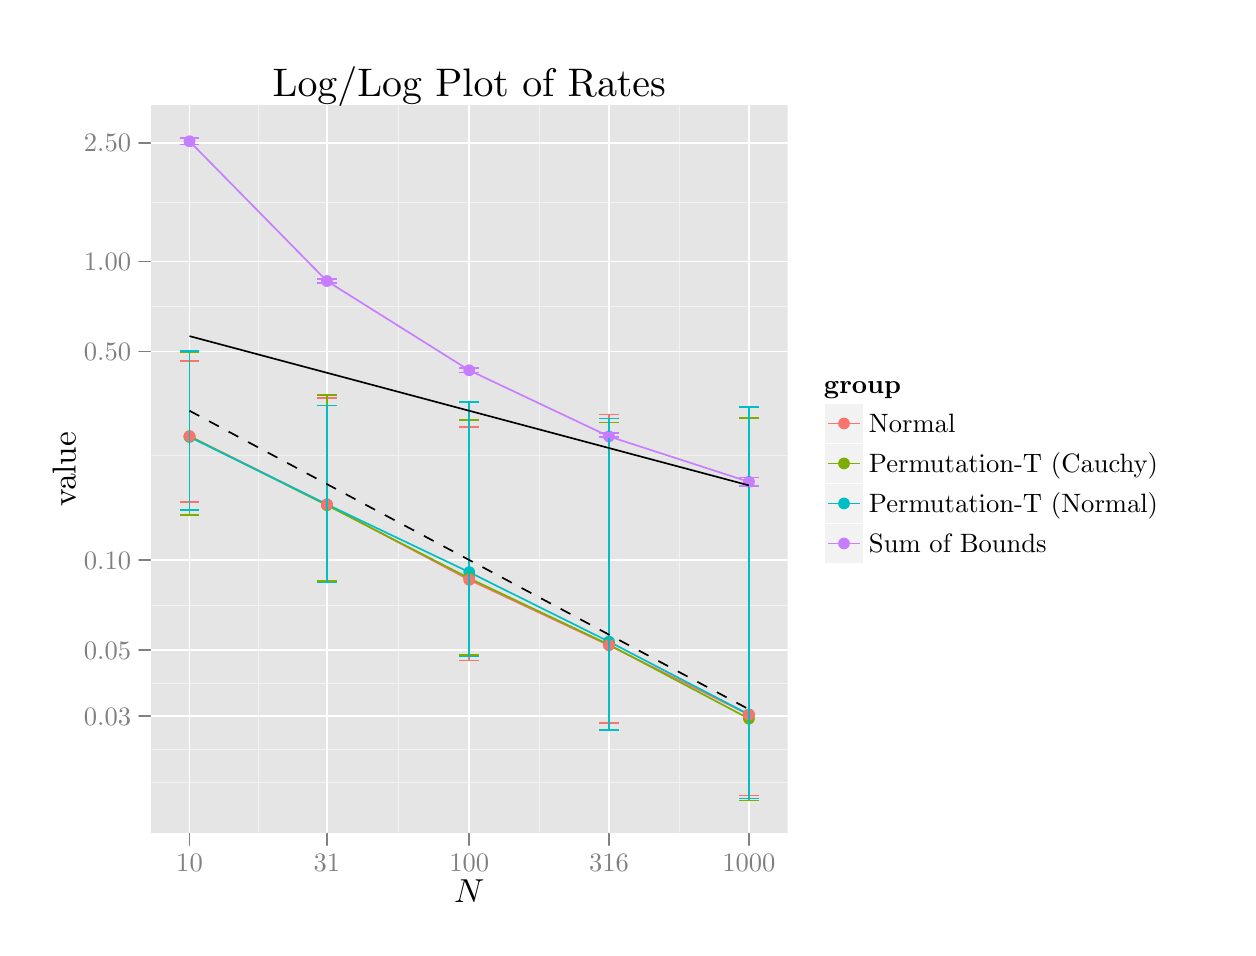
\begin{tikzpicture}[x=1pt,y=1pt]
\definecolor[named]{drawColor}{rgb}{0.00,0.00,0.00}
\definecolor[named]{fillColor}{rgb}{1.00,1.00,1.00}
\fill[color=fillColor,fill opacity=0.00,] (0,0) rectangle (433.62,325.21);
\begin{scope}
\path[clip] (  0.00,  0.00) rectangle (433.62,325.21);
\definecolor[named]{drawColor}{rgb}{0.41,0.16,0.58}
\end{scope}
\begin{scope}
\path[clip] (  0.00,  0.00) rectangle (433.62,325.21);
\definecolor[named]{drawColor}{rgb}{0.41,0.16,0.58}
\end{scope}
\begin{scope}
\path[clip] (  0.00,  0.00) rectangle (433.62,325.21);
\definecolor[named]{drawColor}{rgb}{0.41,0.16,0.58}
\end{scope}
\begin{scope}
\path[clip] (  0.00,  0.00) rectangle (433.62,325.21);
\definecolor[named]{drawColor}{rgb}{0.41,0.16,0.58}
\end{scope}
\begin{scope}
\path[clip] (  0.00,  0.00) rectangle (433.62,325.21);
\definecolor[named]{drawColor}{rgb}{0.41,0.16,0.58}
\end{scope}
\begin{scope}
\path[clip] (  0.00,  0.00) rectangle (433.62,325.21);
\definecolor[named]{drawColor}{rgb}{0.41,0.16,0.58}
\end{scope}
\begin{scope}
\path[clip] (  0.00,  0.00) rectangle (433.62,325.21);
\definecolor[named]{drawColor}{rgb}{0.41,0.16,0.58}
\end{scope}
\begin{scope}
\path[clip] (  0.00,  0.00) rectangle (433.62,325.21);
\definecolor[named]{drawColor}{rgb}{0.41,0.16,0.58}
\end{scope}
\begin{scope}
\path[clip] (  0.00,  0.00) rectangle (433.62,325.21);
\definecolor[named]{drawColor}{rgb}{0.41,0.16,0.58}
\end{scope}
\begin{scope}
\path[clip] (  0.00,  0.00) rectangle (433.62,325.21);
\definecolor[named]{drawColor}{rgb}{0.41,0.16,0.58}
\end{scope}
\begin{scope}
\path[clip] (  0.00,  0.00) rectangle (433.62,325.21);
\definecolor[named]{drawColor}{rgb}{0.41,0.16,0.58}
\end{scope}
\begin{scope}
\path[clip] (  0.00,  0.00) rectangle (433.62,325.21);
\definecolor[named]{drawColor}{rgb}{0.41,0.16,0.58}
\end{scope}
\begin{scope}
\path[clip] ( 44.49, 34.03) rectangle (274.61,297.23);
\definecolor[named]{drawColor}{rgb}{0.41,0.16,0.58}
\end{scope}
\begin{scope}
\path[clip] (  0.00,  0.00) rectangle (433.62,325.21);
\definecolor[named]{drawColor}{rgb}{0.41,0.16,0.58}
\end{scope}
\begin{scope}
\path[clip] (  0.00,  0.00) rectangle (433.62,325.21);
\definecolor[named]{drawColor}{rgb}{0.41,0.16,0.58}
\end{scope}
\begin{scope}
\path[clip] (  0.00,  0.00) rectangle (433.62,325.21);
\definecolor[named]{drawColor}{rgb}{0.41,0.16,0.58}
\end{scope}
\begin{scope}
\path[clip] (  0.00,  0.00) rectangle (433.62,325.21);
\definecolor[named]{drawColor}{rgb}{0.41,0.16,0.58}
\end{scope}
\begin{scope}
\path[clip] (  0.00,  0.00) rectangle (433.62,325.21);
\definecolor[named]{drawColor}{rgb}{0.41,0.16,0.58}
\end{scope}
\begin{scope}
\path[clip] (  0.00,  0.00) rectangle (433.62,325.21);
\definecolor[named]{drawColor}{rgb}{0.41,0.16,0.58}
\end{scope}
\begin{scope}
\path[clip] (  0.00,  0.00) rectangle (433.62,325.21);
\definecolor[named]{drawColor}{rgb}{0.41,0.16,0.58}
\end{scope}
\begin{scope}
\path[clip] (  0.00,  0.00) rectangle (433.62,325.21);
\definecolor[named]{drawColor}{rgb}{0.41,0.16,0.58}
\end{scope}
\begin{scope}
\path[clip] (  0.00,  0.00) rectangle (433.62,325.21);
\definecolor[named]{drawColor}{rgb}{0.41,0.16,0.58}
\end{scope}
\begin{scope}
\path[clip] (  0.00,  0.00) rectangle (433.62,325.21);
\definecolor[named]{drawColor}{rgb}{0.41,0.16,0.58}
\end{scope}
\begin{scope}
\path[clip] (  0.00,  0.00) rectangle (433.62,325.21);
\definecolor[named]{drawColor}{rgb}{0.41,0.16,0.58}
\end{scope}
\begin{scope}
\path[clip] (  0.00,  0.00) rectangle (433.62,325.21);
\definecolor[named]{drawColor}{rgb}{0.41,0.16,0.58}
\definecolor[named]{fillColor}{rgb}{1.00,1.00,1.00}

\draw[fill=fillColor,draw opacity=0.00,] (  0.00,  0.00) rectangle (433.62,325.21);
\end{scope}
\begin{scope}
\path[clip] (  0.00,  0.00) rectangle (433.62,325.21);
\definecolor[named]{drawColor}{rgb}{0.41,0.16,0.58}
\end{scope}
\begin{scope}
\path[clip] (  0.00,  0.00) rectangle (433.62,325.21);
\definecolor[named]{drawColor}{rgb}{0.41,0.16,0.58}
\definecolor[named]{drawColor}{rgb}{0.50,0.50,0.50}

\node[color=drawColor,anchor=base east,inner sep=0pt, outer sep=0pt, scale=  0.96] at ( 37.37, 73.13) {0.03};

\node[color=drawColor,anchor=base east,inner sep=0pt, outer sep=0pt, scale=  0.96] at ( 37.37, 97.07) {0.05};

\node[color=drawColor,anchor=base east,inner sep=0pt, outer sep=0pt, scale=  0.96] at ( 37.37,129.54) {0.10};

\node[color=drawColor,anchor=base east,inner sep=0pt, outer sep=0pt, scale=  0.96] at ( 37.37,204.94) {0.50};

\node[color=drawColor,anchor=base east,inner sep=0pt, outer sep=0pt, scale=  0.96] at ( 37.37,237.42) {1.00};

\node[color=drawColor,anchor=base east,inner sep=0pt, outer sep=0pt, scale=  0.96] at ( 37.37,280.34) {2.50};
\end{scope}
\begin{scope}
\path[clip] (  0.00,  0.00) rectangle (433.62,325.21);
\definecolor[named]{drawColor}{rgb}{0.41,0.16,0.58}
\definecolor[named]{drawColor}{rgb}{0.50,0.50,0.50}

\draw[color=drawColor,line width= 0.6pt,line cap=round,line join=round,fill opacity=0.00,] ( 40.22, 76.44) -- ( 44.49, 76.44);

\draw[color=drawColor,line width= 0.6pt,line cap=round,line join=round,fill opacity=0.00,] ( 40.22,100.37) -- ( 44.49,100.37);

\draw[color=drawColor,line width= 0.6pt,line cap=round,line join=round,fill opacity=0.00,] ( 40.22,132.85) -- ( 44.49,132.85);

\draw[color=drawColor,line width= 0.6pt,line cap=round,line join=round,fill opacity=0.00,] ( 40.22,208.25) -- ( 44.49,208.25);

\draw[color=drawColor,line width= 0.6pt,line cap=round,line join=round,fill opacity=0.00,] ( 40.22,240.72) -- ( 44.49,240.72);

\draw[color=drawColor,line width= 0.6pt,line cap=round,line join=round,fill opacity=0.00,] ( 40.22,283.65) -- ( 44.49,283.65);
\end{scope}
\begin{scope}
\path[clip] (  0.00,  0.00) rectangle (433.62,325.21);
\definecolor[named]{drawColor}{rgb}{0.41,0.16,0.58}
\end{scope}
\begin{scope}
\path[clip] (  0.00,  0.00) rectangle (433.62,325.21);
\definecolor[named]{drawColor}{rgb}{0.41,0.16,0.58}
\end{scope}
\begin{scope}
\path[clip] (  0.00,  0.00) rectangle (433.62,325.21);
\definecolor[named]{drawColor}{rgb}{0.41,0.16,0.58}
\end{scope}
\begin{scope}
\path[clip] (  0.00,  0.00) rectangle (433.62,325.21);
\definecolor[named]{drawColor}{rgb}{0.41,0.16,0.58}
\end{scope}
\begin{scope}
\path[clip] (  0.00,  0.00) rectangle (433.62,325.21);
\definecolor[named]{drawColor}{rgb}{0.41,0.16,0.58}
\end{scope}
\begin{scope}
\path[clip] ( 44.49, 34.03) rectangle (274.61,297.23);
\definecolor[named]{drawColor}{rgb}{0.41,0.16,0.58}
\definecolor[named]{fillColor}{rgb}{0.90,0.90,0.90}

\draw[fill=fillColor,draw opacity=0.00,] ( 44.49, 34.03) rectangle (274.61,297.23);
\definecolor[named]{drawColor}{rgb}{0.95,0.95,0.95}

\draw[color=drawColor,line width= 0.3pt,line cap=round,line join=round,fill opacity=0.00,] ( 44.49, 52.51) --
	(274.61, 52.51);

\draw[color=drawColor,line width= 0.3pt,line cap=round,line join=round,fill opacity=0.00,] ( 44.49, 64.47) --
	(274.61, 64.47);

\draw[color=drawColor,line width= 0.3pt,line cap=round,line join=round,fill opacity=0.00,] ( 44.49, 88.41) --
	(274.61, 88.41);

\draw[color=drawColor,line width= 0.3pt,line cap=round,line join=round,fill opacity=0.00,] ( 44.49,116.61) --
	(274.61,116.61);

\draw[color=drawColor,line width= 0.3pt,line cap=round,line join=round,fill opacity=0.00,] ( 44.49,170.55) --
	(274.61,170.55);

\draw[color=drawColor,line width= 0.3pt,line cap=round,line join=round,fill opacity=0.00,] ( 44.49,224.49) --
	(274.61,224.49);

\draw[color=drawColor,line width= 0.3pt,line cap=round,line join=round,fill opacity=0.00,] ( 44.49,262.19) --
	(274.61,262.19);

\draw[color=drawColor,line width= 0.3pt,line cap=round,line join=round,fill opacity=0.00,] ( 83.31, 34.03) --
	( 83.31,297.23);

\draw[color=drawColor,line width= 0.3pt,line cap=round,line join=round,fill opacity=0.00,] (133.85, 34.03) --
	(133.85,297.23);

\draw[color=drawColor,line width= 0.3pt,line cap=round,line join=round,fill opacity=0.00,] (184.80, 34.03) --
	(184.80,297.23);

\draw[color=drawColor,line width= 0.3pt,line cap=round,line join=round,fill opacity=0.00,] (235.33, 34.03) --
	(235.33,297.23);
\definecolor[named]{drawColor}{rgb}{1.00,1.00,1.00}

\draw[color=drawColor,line width= 0.6pt,line cap=round,line join=round,fill opacity=0.00,] ( 44.49, 76.44) --
	(274.61, 76.44);

\draw[color=drawColor,line width= 0.6pt,line cap=round,line join=round,fill opacity=0.00,] ( 44.49,100.37) --
	(274.61,100.37);

\draw[color=drawColor,line width= 0.6pt,line cap=round,line join=round,fill opacity=0.00,] ( 44.49,132.85) --
	(274.61,132.85);

\draw[color=drawColor,line width= 0.6pt,line cap=round,line join=round,fill opacity=0.00,] ( 44.49,208.25) --
	(274.61,208.25);

\draw[color=drawColor,line width= 0.6pt,line cap=round,line join=round,fill opacity=0.00,] ( 44.49,240.72) --
	(274.61,240.72);

\draw[color=drawColor,line width= 0.6pt,line cap=round,line join=round,fill opacity=0.00,] ( 44.49,283.65) --
	(274.61,283.65);

\draw[color=drawColor,line width= 0.6pt,line cap=round,line join=round,fill opacity=0.00,] ( 58.48, 34.03) --
	( 58.48,297.23);

\draw[color=drawColor,line width= 0.6pt,line cap=round,line join=round,fill opacity=0.00,] (108.14, 34.03) --
	(108.14,297.23);

\draw[color=drawColor,line width= 0.6pt,line cap=round,line join=round,fill opacity=0.00,] (159.55, 34.03) --
	(159.55,297.23);

\draw[color=drawColor,line width= 0.6pt,line cap=round,line join=round,fill opacity=0.00,] (210.05, 34.03) --
	(210.05,297.23);

\draw[color=drawColor,line width= 0.6pt,line cap=round,line join=round,fill opacity=0.00,] (260.62, 34.03) --
	(260.62,297.23);
\definecolor[named]{drawColor}{rgb}{0.97,0.46,0.43}

\draw[color=drawColor,line width= 0.6pt,line join=round,fill opacity=0.00,] ( 58.48,177.61) --
	(108.14,152.89) --
	(159.55,125.69) --
	(210.05,102.01) --
	(260.62, 76.96);
\definecolor[named]{drawColor}{rgb}{0.49,0.68,0.00}

\draw[color=drawColor,line width= 0.6pt,line join=round,fill opacity=0.00,] ( 58.48,177.55) --
	(108.14,152.64) --
	(159.55,126.25) --
	(210.05,102.26) --
	(260.62, 75.52);
\definecolor[named]{drawColor}{rgb}{0.00,0.75,0.77}

\draw[color=drawColor,line width= 0.6pt,line join=round,fill opacity=0.00,] ( 58.48,177.31) --
	(108.14,152.96) --
	(159.55,128.45) --
	(210.05,103.35) --
	(260.62, 77.05);
\definecolor[named]{drawColor}{rgb}{0.78,0.49,1.00}

\draw[color=drawColor,line width= 0.6pt,line join=round,fill opacity=0.00,] ( 58.48,284.15) --
	(108.14,233.65) --
	(159.55,201.40) --
	(210.05,177.51) --
	(260.62,161.10);
\definecolor[named]{fillColor}{rgb}{0.00,0.75,0.77}

\draw[fill=fillColor,draw opacity=0.00,] ( 58.48,177.31) circle (  2.13);
\definecolor[named]{fillColor}{rgb}{0.49,0.68,0.00}

\draw[fill=fillColor,draw opacity=0.00,] ( 58.48,177.55) circle (  2.13);
\definecolor[named]{fillColor}{rgb}{0.97,0.46,0.43}

\draw[fill=fillColor,draw opacity=0.00,] ( 58.48,177.61) circle (  2.13);
\definecolor[named]{fillColor}{rgb}{0.00,0.75,0.77}

\draw[fill=fillColor,draw opacity=0.00,] (108.14,152.96) circle (  2.13);
\definecolor[named]{fillColor}{rgb}{0.49,0.68,0.00}

\draw[fill=fillColor,draw opacity=0.00,] (108.14,152.64) circle (  2.13);
\definecolor[named]{fillColor}{rgb}{0.97,0.46,0.43}

\draw[fill=fillColor,draw opacity=0.00,] (108.14,152.89) circle (  2.13);
\definecolor[named]{fillColor}{rgb}{0.00,0.75,0.77}

\draw[fill=fillColor,draw opacity=0.00,] (159.55,128.45) circle (  2.13);
\definecolor[named]{fillColor}{rgb}{0.49,0.68,0.00}

\draw[fill=fillColor,draw opacity=0.00,] (159.55,126.25) circle (  2.13);
\definecolor[named]{fillColor}{rgb}{0.97,0.46,0.43}

\draw[fill=fillColor,draw opacity=0.00,] (159.55,125.69) circle (  2.13);
\definecolor[named]{fillColor}{rgb}{0.00,0.75,0.77}

\draw[fill=fillColor,draw opacity=0.00,] (210.05,103.35) circle (  2.13);
\definecolor[named]{fillColor}{rgb}{0.49,0.68,0.00}

\draw[fill=fillColor,draw opacity=0.00,] (210.05,102.26) circle (  2.13);
\definecolor[named]{fillColor}{rgb}{0.97,0.46,0.43}

\draw[fill=fillColor,draw opacity=0.00,] (210.05,102.01) circle (  2.13);
\definecolor[named]{fillColor}{rgb}{0.00,0.75,0.77}

\draw[fill=fillColor,draw opacity=0.00,] (260.62, 77.05) circle (  2.13);
\definecolor[named]{fillColor}{rgb}{0.49,0.68,0.00}

\draw[fill=fillColor,draw opacity=0.00,] (260.62, 75.52) circle (  2.13);
\definecolor[named]{fillColor}{rgb}{0.97,0.46,0.43}

\draw[fill=fillColor,draw opacity=0.00,] (260.62, 76.96) circle (  2.13);
\definecolor[named]{fillColor}{rgb}{0.78,0.49,1.00}

\draw[fill=fillColor,draw opacity=0.00,] ( 58.48,284.15) circle (  2.13);

\draw[fill=fillColor,draw opacity=0.00,] (108.14,233.65) circle (  2.13);

\draw[fill=fillColor,draw opacity=0.00,] (159.55,201.40) circle (  2.13);

\draw[fill=fillColor,draw opacity=0.00,] (210.05,177.51) circle (  2.13);

\draw[fill=fillColor,draw opacity=0.00,] (260.62,161.10) circle (  2.13);
\definecolor[named]{drawColor}{rgb}{0.97,0.46,0.43}

\draw[color=drawColor,line width= 0.6pt,line join=round,fill opacity=0.00,] ( 54.95,204.74) --
	( 62.02,204.74);

\draw[color=drawColor,line width= 0.6pt,line join=round,fill opacity=0.00,] ( 58.48,204.74) --
	( 58.48,153.80);

\draw[color=drawColor,line width= 0.6pt,line join=round,fill opacity=0.00,] ( 54.95,153.80) --
	( 62.02,153.80);

\draw[color=drawColor,line width= 0.6pt,line join=round,fill opacity=0.00,] (104.61,191.45) --
	(111.68,191.45);

\draw[color=drawColor,line width= 0.6pt,line join=round,fill opacity=0.00,] (108.14,191.45) --
	(108.14,125.00);

\draw[color=drawColor,line width= 0.6pt,line join=round,fill opacity=0.00,] (104.61,125.00) --
	(111.68,125.00);

\draw[color=drawColor,line width= 0.6pt,line join=round,fill opacity=0.00,] (156.01,181.01) --
	(163.09,181.01);

\draw[color=drawColor,line width= 0.6pt,line join=round,fill opacity=0.00,] (159.55,181.01) --
	(159.55, 96.56);

\draw[color=drawColor,line width= 0.6pt,line join=round,fill opacity=0.00,] (156.01, 96.56) --
	(163.09, 96.56);

\draw[color=drawColor,line width= 0.6pt,line join=round,fill opacity=0.00,] (206.51,185.42) --
	(213.59,185.42);

\draw[color=drawColor,line width= 0.6pt,line join=round,fill opacity=0.00,] (210.05,185.42) --
	(210.05, 73.96);

\draw[color=drawColor,line width= 0.6pt,line join=round,fill opacity=0.00,] (206.51, 73.96) --
	(213.59, 73.96);

\draw[color=drawColor,line width= 0.6pt,line join=round,fill opacity=0.00,] (257.08,184.36) --
	(264.15,184.36);

\draw[color=drawColor,line width= 0.6pt,line join=round,fill opacity=0.00,] (260.62,184.36) --
	(260.62, 47.72);

\draw[color=drawColor,line width= 0.6pt,line join=round,fill opacity=0.00,] (257.08, 47.72) --
	(264.15, 47.72);
\definecolor[named]{drawColor}{rgb}{0.49,0.68,0.00}

\draw[color=drawColor,line width= 0.6pt,line join=round,fill opacity=0.00,] ( 54.95,207.80) --
	( 62.02,207.80);

\draw[color=drawColor,line width= 0.6pt,line join=round,fill opacity=0.00,] ( 58.48,207.80) --
	( 58.48,149.16);

\draw[color=drawColor,line width= 0.6pt,line join=round,fill opacity=0.00,] ( 54.95,149.16) --
	( 62.02,149.16);

\draw[color=drawColor,line width= 0.6pt,line join=round,fill opacity=0.00,] (104.61,192.36) --
	(111.68,192.36);

\draw[color=drawColor,line width= 0.6pt,line join=round,fill opacity=0.00,] (108.14,192.36) --
	(108.14,125.24);

\draw[color=drawColor,line width= 0.6pt,line join=round,fill opacity=0.00,] (104.61,125.24) --
	(111.68,125.24);

\draw[color=drawColor,line width= 0.6pt,line join=round,fill opacity=0.00,] (156.01,183.42) --
	(163.09,183.42);

\draw[color=drawColor,line width= 0.6pt,line join=round,fill opacity=0.00,] (159.55,183.42) --
	(159.55, 98.53);

\draw[color=drawColor,line width= 0.6pt,line join=round,fill opacity=0.00,] (156.01, 98.53) --
	(163.09, 98.53);

\draw[color=drawColor,line width= 0.6pt,line join=round,fill opacity=0.00,] (206.51,182.54) --
	(213.59,182.54);

\draw[color=drawColor,line width= 0.6pt,line join=round,fill opacity=0.00,] (210.05,182.54) --
	(210.05, 71.65);

\draw[color=drawColor,line width= 0.6pt,line join=round,fill opacity=0.00,] (206.51, 71.65) --
	(213.59, 71.65);

\draw[color=drawColor,line width= 0.6pt,line join=round,fill opacity=0.00,] (257.08,184.20) --
	(264.15,184.20);

\draw[color=drawColor,line width= 0.6pt,line join=round,fill opacity=0.00,] (260.62,184.20) --
	(260.62, 46.00);

\draw[color=drawColor,line width= 0.6pt,line join=round,fill opacity=0.00,] (257.08, 46.00) --
	(264.15, 46.00);
\definecolor[named]{drawColor}{rgb}{0.00,0.75,0.77}

\draw[color=drawColor,line width= 0.6pt,line join=round,fill opacity=0.00,] ( 54.95,208.27) --
	( 62.02,208.27);

\draw[color=drawColor,line width= 0.6pt,line join=round,fill opacity=0.00,] ( 58.48,208.27) --
	( 58.48,150.80);

\draw[color=drawColor,line width= 0.6pt,line join=round,fill opacity=0.00,] ( 54.95,150.80) --
	( 62.02,150.80);

\draw[color=drawColor,line width= 0.6pt,line join=round,fill opacity=0.00,] (104.61,188.64) --
	(111.68,188.64);

\draw[color=drawColor,line width= 0.6pt,line join=round,fill opacity=0.00,] (108.14,188.64) --
	(108.14,124.72);

\draw[color=drawColor,line width= 0.6pt,line join=round,fill opacity=0.00,] (104.61,124.72) --
	(111.68,124.72);

\draw[color=drawColor,line width= 0.6pt,line join=round,fill opacity=0.00,] (156.01,189.99) --
	(163.09,189.99);

\draw[color=drawColor,line width= 0.6pt,line join=round,fill opacity=0.00,] (159.55,189.99) --
	(159.55, 98.00);

\draw[color=drawColor,line width= 0.6pt,line join=round,fill opacity=0.00,] (156.01, 98.00) --
	(163.09, 98.00);

\draw[color=drawColor,line width= 0.6pt,line join=round,fill opacity=0.00,] (206.51,183.95) --
	(213.59,183.95);

\draw[color=drawColor,line width= 0.6pt,line join=round,fill opacity=0.00,] (210.05,183.95) --
	(210.05, 71.48);

\draw[color=drawColor,line width= 0.6pt,line join=round,fill opacity=0.00,] (206.51, 71.48) --
	(213.59, 71.48);

\draw[color=drawColor,line width= 0.6pt,line join=round,fill opacity=0.00,] (257.08,188.23) --
	(264.15,188.23);

\draw[color=drawColor,line width= 0.6pt,line join=round,fill opacity=0.00,] (260.62,188.23) --
	(260.62, 46.65);

\draw[color=drawColor,line width= 0.6pt,line join=round,fill opacity=0.00,] (257.08, 46.65) --
	(264.15, 46.65);
\definecolor[named]{drawColor}{rgb}{0.78,0.49,1.00}

\draw[color=drawColor,line width= 0.6pt,line join=round,fill opacity=0.00,] ( 54.95,285.27) --
	( 62.02,285.27);

\draw[color=drawColor,line width= 0.6pt,line join=round,fill opacity=0.00,] ( 58.48,285.27) --
	( 58.48,283.02);

\draw[color=drawColor,line width= 0.6pt,line join=round,fill opacity=0.00,] ( 54.95,283.02) --
	( 62.02,283.02);

\draw[color=drawColor,line width= 0.6pt,line join=round,fill opacity=0.00,] (104.61,234.28) --
	(111.68,234.28);

\draw[color=drawColor,line width= 0.6pt,line join=round,fill opacity=0.00,] (108.14,234.28) --
	(108.14,233.01);

\draw[color=drawColor,line width= 0.6pt,line join=round,fill opacity=0.00,] (104.61,233.01) --
	(111.68,233.01);

\draw[color=drawColor,line width= 0.6pt,line join=round,fill opacity=0.00,] (156.01,202.24) --
	(163.09,202.24);

\draw[color=drawColor,line width= 0.6pt,line join=round,fill opacity=0.00,] (159.55,202.24) --
	(159.55,200.59);

\draw[color=drawColor,line width= 0.6pt,line join=round,fill opacity=0.00,] (156.01,200.59) --
	(163.09,200.59);

\draw[color=drawColor,line width= 0.6pt,line join=round,fill opacity=0.00,] (206.51,178.78) --
	(213.59,178.78);

\draw[color=drawColor,line width= 0.6pt,line join=round,fill opacity=0.00,] (210.05,178.78) --
	(210.05,177.26);

\draw[color=drawColor,line width= 0.6pt,line join=round,fill opacity=0.00,] (206.51,177.26) --
	(213.59,177.26);

\draw[color=drawColor,line width= 0.6pt,line join=round,fill opacity=0.00,] (257.08,162.61) --
	(264.15,162.61);

\draw[color=drawColor,line width= 0.6pt,line join=round,fill opacity=0.00,] (260.62,162.61) --
	(260.62,159.55);

\draw[color=drawColor,line width= 0.6pt,line join=round,fill opacity=0.00,] (257.08,159.55) --
	(264.15,159.55);
\definecolor[named]{drawColor}{rgb}{0.00,0.00,0.00}

\draw[color=drawColor,line width= 0.6pt,dash pattern=on 4pt off 4pt ,line join=round,fill opacity=0.00,] ( 58.48,186.78) --
	( 58.48,186.78) --
	( 58.48,186.78) --
	( 58.48,186.78) --
	(108.14,160.28) --
	(108.14,160.28) --
	(108.14,160.28) --
	(108.14,160.28) --
	(159.55,132.85) --
	(159.55,132.85) --
	(159.55,132.85) --
	(159.55,132.85) --
	(210.05,105.89) --
	(210.05,105.89) --
	(210.05,105.89) --
	(210.05,105.89) --
	(260.62, 78.91) --
	(260.62, 78.91) --
	(260.62, 78.91) --
	(260.62, 78.91);

\draw[color=drawColor,line width= 0.6pt,line join=round,fill opacity=0.00,] ( 58.48,213.75) --
	( 58.48,213.75) --
	( 58.48,213.75) --
	( 58.48,213.75) --
	(108.14,200.50) --
	(108.14,200.50) --
	(108.14,200.50) --
	(108.14,200.50) --
	(159.55,186.78) --
	(159.55,186.78) --
	(159.55,186.78) --
	(159.55,186.78) --
	(210.05,173.31) --
	(210.05,173.31) --
	(210.05,173.31) --
	(210.05,173.31) --
	(260.62,159.82) --
	(260.62,159.82) --
	(260.62,159.82) --
	(260.62,159.82);
\end{scope}
\begin{scope}
\path[clip] (  0.00,  0.00) rectangle (433.62,325.21);
\definecolor[named]{drawColor}{rgb}{0.41,0.16,0.58}
\end{scope}
\begin{scope}
\path[clip] (  0.00,  0.00) rectangle (433.62,325.21);
\definecolor[named]{drawColor}{rgb}{0.41,0.16,0.58}
\definecolor[named]{drawColor}{rgb}{0.50,0.50,0.50}

\node[color=drawColor,anchor=base,inner sep=0pt, outer sep=0pt, scale=  0.96] at ( 58.48, 20.31) {10};

\node[color=drawColor,anchor=base,inner sep=0pt, outer sep=0pt, scale=  0.96] at (108.14, 20.31) {31};

\node[color=drawColor,anchor=base,inner sep=0pt, outer sep=0pt, scale=  0.96] at (159.55, 20.31) {100};

\node[color=drawColor,anchor=base,inner sep=0pt, outer sep=0pt, scale=  0.96] at (210.05, 20.31) {316};

\node[color=drawColor,anchor=base,inner sep=0pt, outer sep=0pt, scale=  0.96] at (260.62, 20.31) {1000};
\end{scope}
\begin{scope}
\path[clip] (  0.00,  0.00) rectangle (433.62,325.21);
\definecolor[named]{drawColor}{rgb}{0.41,0.16,0.58}
\definecolor[named]{drawColor}{rgb}{0.50,0.50,0.50}

\draw[color=drawColor,line width= 0.6pt,line cap=round,line join=round,fill opacity=0.00,] ( 58.48, 29.77) -- ( 58.48, 34.03);

\draw[color=drawColor,line width= 0.6pt,line cap=round,line join=round,fill opacity=0.00,] (108.14, 29.77) -- (108.14, 34.03);

\draw[color=drawColor,line width= 0.6pt,line cap=round,line join=round,fill opacity=0.00,] (159.55, 29.77) -- (159.55, 34.03);

\draw[color=drawColor,line width= 0.6pt,line cap=round,line join=round,fill opacity=0.00,] (210.05, 29.77) -- (210.05, 34.03);

\draw[color=drawColor,line width= 0.6pt,line cap=round,line join=round,fill opacity=0.00,] (260.62, 29.77) -- (260.62, 34.03);
\end{scope}
\begin{scope}
\path[clip] (  0.00,  0.00) rectangle (433.62,325.21);
\definecolor[named]{drawColor}{rgb}{0.41,0.16,0.58}
\end{scope}
\begin{scope}
\path[clip] (  0.00,  0.00) rectangle (433.62,325.21);
\definecolor[named]{drawColor}{rgb}{0.41,0.16,0.58}
\end{scope}
\begin{scope}
\path[clip] (  0.00,  0.00) rectangle (433.62,325.21);
\definecolor[named]{drawColor}{rgb}{0.41,0.16,0.58}
\end{scope}
\begin{scope}
\path[clip] (  0.00,  0.00) rectangle (433.62,325.21);
\definecolor[named]{drawColor}{rgb}{0.41,0.16,0.58}
\definecolor[named]{drawColor}{rgb}{0.00,0.00,0.00}

\node[color=drawColor,anchor=base,inner sep=0pt, outer sep=0pt, scale=  1.44] at (159.55,300.24) {Log/Log Plot of Rates};
\end{scope}
\begin{scope}
\path[clip] (  0.00,  0.00) rectangle (433.62,325.21);
\definecolor[named]{drawColor}{rgb}{0.41,0.16,0.58}
\end{scope}
\begin{scope}
\path[clip] (  0.00,  0.00) rectangle (433.62,325.21);
\definecolor[named]{drawColor}{rgb}{0.41,0.16,0.58}
\definecolor[named]{drawColor}{rgb}{0.00,0.00,0.00}

\node[color=drawColor,anchor=base,inner sep=0pt, outer sep=0pt, scale=  1.20] at (159.55,  9.03) {$N$};
\end{scope}
\begin{scope}
\path[clip] (  0.00,  0.00) rectangle (433.62,325.21);
\definecolor[named]{drawColor}{rgb}{0.41,0.16,0.58}
\end{scope}
\begin{scope}
\path[clip] (  0.00,  0.00) rectangle (433.62,325.21);
\definecolor[named]{drawColor}{rgb}{0.41,0.16,0.58}
\definecolor[named]{drawColor}{rgb}{0.00,0.00,0.00}

\node[rotate= 90.00,color=drawColor,anchor=base,inner sep=0pt, outer sep=0pt, scale=  1.20] at ( 17.30,165.63) {value};
\end{scope}
\begin{scope}
\path[clip] (  0.00,  0.00) rectangle (433.62,325.21);
\definecolor[named]{drawColor}{rgb}{0.41,0.16,0.58}
\end{scope}
\begin{scope}
\path[clip] (  0.00,  0.00) rectangle (433.62,325.21);
\definecolor[named]{drawColor}{rgb}{0.41,0.16,0.58}
\end{scope}
\begin{scope}
\path[clip] (  0.00,  0.00) rectangle (433.62,325.21);
\definecolor[named]{drawColor}{rgb}{0.41,0.16,0.58}
\end{scope}
\begin{scope}
\path[clip] (  0.00,  0.00) rectangle (433.62,325.21);
\definecolor[named]{drawColor}{rgb}{0.41,0.16,0.58}
\end{scope}
\begin{scope}
\path[clip] (  0.00,  0.00) rectangle (433.62,325.21);
\definecolor[named]{drawColor}{rgb}{0.41,0.16,0.58}
\end{scope}
\begin{scope}
\path[clip] (  0.00,  0.00) rectangle (433.62,325.21);
\definecolor[named]{drawColor}{rgb}{0.41,0.16,0.58}
\end{scope}
\begin{scope}
\path[clip] (  0.00,  0.00) rectangle (433.62,325.21);
\definecolor[named]{drawColor}{rgb}{0.41,0.16,0.58}
\end{scope}
\begin{scope}
\path[clip] (  0.00,  0.00) rectangle (433.62,325.21);
\definecolor[named]{drawColor}{rgb}{0.41,0.16,0.58}
\end{scope}
\begin{scope}
\path[clip] (  0.00,  0.00) rectangle (433.62,325.21);
\definecolor[named]{drawColor}{rgb}{0.41,0.16,0.58}
\end{scope}
\begin{scope}
\path[clip] (  0.00,  0.00) rectangle (433.62,325.21);
\definecolor[named]{drawColor}{rgb}{0.41,0.16,0.58}
\end{scope}
\begin{scope}
\path[clip] (  0.00,  0.00) rectangle (433.62,325.21);
\definecolor[named]{drawColor}{rgb}{0.41,0.16,0.58}
\end{scope}
\begin{scope}
\path[clip] (  0.00,  0.00) rectangle (433.62,325.21);
\definecolor[named]{drawColor}{rgb}{0.41,0.16,0.58}
\end{scope}
\begin{scope}
\path[clip] (  0.00,  0.00) rectangle (433.62,325.21);
\definecolor[named]{drawColor}{rgb}{0.41,0.16,0.58}
\end{scope}
\begin{scope}
\path[clip] (  0.00,  0.00) rectangle (433.62,325.21);
\definecolor[named]{drawColor}{rgb}{0.41,0.16,0.58}
\end{scope}
\begin{scope}
\path[clip] (  0.00,  0.00) rectangle (433.62,325.21);
\definecolor[named]{drawColor}{rgb}{0.41,0.16,0.58}
\end{scope}
\begin{scope}
\path[clip] (  0.00,  0.00) rectangle (433.62,325.21);
\definecolor[named]{drawColor}{rgb}{0.41,0.16,0.58}
\end{scope}
\begin{scope}
\path[clip] (  0.00,  0.00) rectangle (433.62,325.21);
\definecolor[named]{drawColor}{rgb}{0.41,0.16,0.58}
\end{scope}
\begin{scope}
\path[clip] (  0.00,  0.00) rectangle (433.62,325.21);
\definecolor[named]{drawColor}{rgb}{0.41,0.16,0.58}
\end{scope}
\begin{scope}
\path[clip] (  0.00,  0.00) rectangle (433.62,325.21);
\definecolor[named]{drawColor}{rgb}{0.41,0.16,0.58}
\end{scope}
\begin{scope}
\path[clip] (  0.00,  0.00) rectangle (433.62,325.21);
\definecolor[named]{drawColor}{rgb}{0.41,0.16,0.58}
\end{scope}
\begin{scope}
\path[clip] (  0.00,  0.00) rectangle (433.62,325.21);
\definecolor[named]{drawColor}{rgb}{0.41,0.16,0.58}
\end{scope}
\begin{scope}
\path[clip] (  0.00,  0.00) rectangle (433.62,325.21);
\definecolor[named]{drawColor}{rgb}{0.41,0.16,0.58}
\end{scope}
\begin{scope}
\path[clip] (  0.00,  0.00) rectangle (433.62,325.21);
\definecolor[named]{drawColor}{rgb}{0.41,0.16,0.58}
\end{scope}
\begin{scope}
\path[clip] (  0.00,  0.00) rectangle (433.62,325.21);
\definecolor[named]{drawColor}{rgb}{0.41,0.16,0.58}
\end{scope}
\begin{scope}
\path[clip] (  0.00,  0.00) rectangle (433.62,325.21);
\definecolor[named]{drawColor}{rgb}{0.41,0.16,0.58}
\definecolor[named]{drawColor}{rgb}{1.00,1.00,1.00}

\draw[color=drawColor,line width= 0.6pt,line cap=round,line join=round,fill opacity=0.00,] (283.48,127.34) rectangle (412.71,203.93);
\end{scope}
\begin{scope}
\path[clip] (  0.00,  0.00) rectangle (433.62,325.21);
\definecolor[named]{drawColor}{rgb}{0.41,0.16,0.58}
\definecolor[named]{drawColor}{rgb}{0.00,0.00,0.00}

\node[color=drawColor,anchor=base west,inner sep=0pt, outer sep=0pt, scale=  0.96] at (287.75,193.03) {\bfseries group};
\end{scope}
\begin{scope}
\path[clip] (  0.00,  0.00) rectangle (433.62,325.21);
\definecolor[named]{drawColor}{rgb}{0.41,0.16,0.58}
\definecolor[named]{drawColor}{rgb}{1.00,1.00,1.00}
\definecolor[named]{fillColor}{rgb}{0.95,0.95,0.95}

\draw[color=drawColor,line width= 0.6pt,line cap=round,line join=round,fill=fillColor,] (287.75,174.97) rectangle (302.20,189.42);
\end{scope}
\begin{scope}
\path[clip] (  0.00,  0.00) rectangle (433.62,325.21);
\definecolor[named]{drawColor}{rgb}{0.41,0.16,0.58}
\definecolor[named]{drawColor}{rgb}{0.97,0.46,0.43}

\draw[color=drawColor,line width= 0.6pt,line join=round,fill opacity=0.00,] (289.20,182.19) -- (300.76,182.19);
\end{scope}
\begin{scope}
\path[clip] (  0.00,  0.00) rectangle (433.62,325.21);
\definecolor[named]{drawColor}{rgb}{0.41,0.16,0.58}
\definecolor[named]{fillColor}{rgb}{0.97,0.46,0.43}

\draw[fill=fillColor,draw opacity=0.00,] (294.98,182.19) circle (  2.13);
\end{scope}
\begin{scope}
\path[clip] (  0.00,  0.00) rectangle (433.62,325.21);
\definecolor[named]{drawColor}{rgb}{0.41,0.16,0.58}
\definecolor[named]{drawColor}{rgb}{0.97,0.46,0.43}

\draw[color=drawColor,line width= 0.6pt,line join=round,fill opacity=0.00,] (289.20,182.19) -- (300.76,182.19);
\end{scope}
\begin{scope}
\path[clip] (  0.00,  0.00) rectangle (433.62,325.21);
\definecolor[named]{drawColor}{rgb}{0.41,0.16,0.58}
\definecolor[named]{drawColor}{rgb}{1.00,1.00,1.00}
\definecolor[named]{fillColor}{rgb}{0.95,0.95,0.95}

\draw[color=drawColor,line width= 0.6pt,line cap=round,line join=round,fill=fillColor,] (287.75,160.51) rectangle (302.20,174.97);
\end{scope}
\begin{scope}
\path[clip] (  0.00,  0.00) rectangle (433.62,325.21);
\definecolor[named]{drawColor}{rgb}{0.41,0.16,0.58}
\definecolor[named]{drawColor}{rgb}{0.49,0.68,0.00}

\draw[color=drawColor,line width= 0.6pt,line join=round,fill opacity=0.00,] (289.20,167.74) -- (300.76,167.74);
\end{scope}
\begin{scope}
\path[clip] (  0.00,  0.00) rectangle (433.62,325.21);
\definecolor[named]{drawColor}{rgb}{0.41,0.16,0.58}
\definecolor[named]{fillColor}{rgb}{0.49,0.68,0.00}

\draw[fill=fillColor,draw opacity=0.00,] (294.98,167.74) circle (  2.13);
\end{scope}
\begin{scope}
\path[clip] (  0.00,  0.00) rectangle (433.62,325.21);
\definecolor[named]{drawColor}{rgb}{0.41,0.16,0.58}
\definecolor[named]{drawColor}{rgb}{0.49,0.68,0.00}

\draw[color=drawColor,line width= 0.6pt,line join=round,fill opacity=0.00,] (289.20,167.74) -- (300.76,167.74);
\end{scope}
\begin{scope}
\path[clip] (  0.00,  0.00) rectangle (433.62,325.21);
\definecolor[named]{drawColor}{rgb}{0.41,0.16,0.58}
\definecolor[named]{drawColor}{rgb}{1.00,1.00,1.00}
\definecolor[named]{fillColor}{rgb}{0.95,0.95,0.95}

\draw[color=drawColor,line width= 0.6pt,line cap=round,line join=round,fill=fillColor,] (287.75,146.06) rectangle (302.20,160.51);
\end{scope}
\begin{scope}
\path[clip] (  0.00,  0.00) rectangle (433.62,325.21);
\definecolor[named]{drawColor}{rgb}{0.41,0.16,0.58}
\definecolor[named]{drawColor}{rgb}{0.00,0.75,0.77}

\draw[color=drawColor,line width= 0.6pt,line join=round,fill opacity=0.00,] (289.20,153.29) -- (300.76,153.29);
\end{scope}
\begin{scope}
\path[clip] (  0.00,  0.00) rectangle (433.62,325.21);
\definecolor[named]{drawColor}{rgb}{0.41,0.16,0.58}
\definecolor[named]{fillColor}{rgb}{0.00,0.75,0.77}

\draw[fill=fillColor,draw opacity=0.00,] (294.98,153.29) circle (  2.13);
\end{scope}
\begin{scope}
\path[clip] (  0.00,  0.00) rectangle (433.62,325.21);
\definecolor[named]{drawColor}{rgb}{0.41,0.16,0.58}
\definecolor[named]{drawColor}{rgb}{0.00,0.75,0.77}

\draw[color=drawColor,line width= 0.6pt,line join=round,fill opacity=0.00,] (289.20,153.29) -- (300.76,153.29);
\end{scope}
\begin{scope}
\path[clip] (  0.00,  0.00) rectangle (433.62,325.21);
\definecolor[named]{drawColor}{rgb}{0.41,0.16,0.58}
\definecolor[named]{drawColor}{rgb}{1.00,1.00,1.00}
\definecolor[named]{fillColor}{rgb}{0.95,0.95,0.95}

\draw[color=drawColor,line width= 0.6pt,line cap=round,line join=round,fill=fillColor,] (287.75,131.60) rectangle (302.20,146.06);
\end{scope}
\begin{scope}
\path[clip] (  0.00,  0.00) rectangle (433.62,325.21);
\definecolor[named]{drawColor}{rgb}{0.41,0.16,0.58}
\definecolor[named]{drawColor}{rgb}{0.78,0.49,1.00}

\draw[color=drawColor,line width= 0.6pt,line join=round,fill opacity=0.00,] (289.20,138.83) -- (300.76,138.83);
\end{scope}
\begin{scope}
\path[clip] (  0.00,  0.00) rectangle (433.62,325.21);
\definecolor[named]{drawColor}{rgb}{0.41,0.16,0.58}
\definecolor[named]{fillColor}{rgb}{0.78,0.49,1.00}

\draw[fill=fillColor,draw opacity=0.00,] (294.98,138.83) circle (  2.13);
\end{scope}
\begin{scope}
\path[clip] (  0.00,  0.00) rectangle (433.62,325.21);
\definecolor[named]{drawColor}{rgb}{0.41,0.16,0.58}
\definecolor[named]{drawColor}{rgb}{0.78,0.49,1.00}

\draw[color=drawColor,line width= 0.6pt,line join=round,fill opacity=0.00,] (289.20,138.83) -- (300.76,138.83);
\end{scope}
\begin{scope}
\path[clip] (  0.00,  0.00) rectangle (433.62,325.21);
\definecolor[named]{drawColor}{rgb}{0.41,0.16,0.58}
\definecolor[named]{drawColor}{rgb}{0.00,0.00,0.00}

\node[color=drawColor,anchor=base west,inner sep=0pt, outer sep=0pt, scale=  0.96] at (304.01,178.89) {Normal};
\end{scope}
\begin{scope}
\path[clip] (  0.00,  0.00) rectangle (433.62,325.21);
\definecolor[named]{drawColor}{rgb}{0.41,0.16,0.58}
\definecolor[named]{drawColor}{rgb}{0.00,0.00,0.00}

\node[color=drawColor,anchor=base west,inner sep=0pt, outer sep=0pt, scale=  0.96] at (304.01,164.43) {Permutation-T (Cauchy)};
\end{scope}
\begin{scope}
\path[clip] (  0.00,  0.00) rectangle (433.62,325.21);
\definecolor[named]{drawColor}{rgb}{0.41,0.16,0.58}
\definecolor[named]{drawColor}{rgb}{0.00,0.00,0.00}

\node[color=drawColor,anchor=base west,inner sep=0pt, outer sep=0pt, scale=  0.96] at (304.01,149.98) {Permutation-T (Normal)};
\end{scope}
\begin{scope}
\path[clip] (  0.00,  0.00) rectangle (433.62,325.21);
\definecolor[named]{drawColor}{rgb}{0.41,0.16,0.58}
\definecolor[named]{drawColor}{rgb}{0.00,0.00,0.00}

\node[color=drawColor,anchor=base west,inner sep=0pt, outer sep=0pt, scale=  0.96] at (304.01,135.53) {Sum of Bounds};
\end{scope}
\begin{scope}
\path[clip] (  0.00,  0.00) rectangle (433.62,325.21);
\definecolor[named]{drawColor}{rgb}{0.41,0.16,0.58}
\end{scope}
\begin{scope}
\path[clip] (  0.00,  0.00) rectangle (433.62,325.21);
\definecolor[named]{drawColor}{rgb}{0.41,0.16,0.58}
\end{scope}
\begin{scope}
\path[clip] (  0.00,  0.00) rectangle (433.62,325.21);
\definecolor[named]{drawColor}{rgb}{0.41,0.16,0.58}
\end{scope}
\end{tikzpicture}

  \caption{Solid black line: $N^{-1/4}$; dashed black line: $N^{-1/2}$}
\end{figure}

It's not a fair comparison to place the sum of the bounds on the same plot because that was computed
over $200,000$ separate permutations instead of the $500$ shared by the other three.  Still, we can
draw some general conclusions.  The normal and two permutation-$t$ K-S statistics decay perfectly at
a rate of $N^{-1/2}$, and our bound follows a rate of $N^{-1/4}$, suggesting that the true rate of
convergence is the former.  Also, the error-bars seem to be increasing in size but are actually
roughly constant due to the log-log scale.

Chen et al. \cite{chen2010normal} provide a simple example
(pp.154-155) in which the sum of i.i.d. random variables yields
\begin{equation*}
  E|W' - W|^3 = \frac{4}{N^{3/2}}
\end{equation*}
with $\lambda = N^{-1}$.  This leads to an $O(N^{-1/4})$ bound, which is suboptimal and apparently
not uncommon when applying this kind of theorem.

\section{Efficient Updates}
Instead of conditioning on the value of $T_{\Pi}$, we condition on the
observed permutation $\pi$.  For $N$ observations in each group, there
are $N^2 \: T_{\Pi}'$ values that come from swapping one value in the first
group with one value in the second.  $T_{\Pi}'$ should not differ much from
$T_{\Pi}$, and calculating the $t$-statistics from scratch is inefficient.  

We use an efficient $t$-statistic update rule to easily calculate
millions of $t$-statistics.  The two sample $t$-statistic is given by
\begin{equation*}
  T_{\Pi} = \frac{\bar{x}-\bar{u}}
  {\sqrt{\frac{2}{n}}\sqrt{\frac{1}{2}(S_X^2+S_U^2)}},
\end{equation*}
where $S_X^2=\frac{1}{N-1}(\sum_{i=1}^Nx_i^2-n\bar{x}^2)$.

Let $T_{x_i,u_j}$ be the result of $T'$ by swapping $x_i$ with $u_j$:
\begin{align*}
  \Delta &\equiv u_j-x_i \\
  \bar{x}_{x_i,u_j} &= \bar{x}-\frac{1}{N}x_i+\frac{1}{N}u_j =
  \bar{x}+\frac{\Delta}{N} \\
  \bar{u}_{x_i,u_j} &= \bar{u}+\frac{1}{N}x_i-\frac{1}{N}u_j =
  \bar{u}-\frac{\Delta}{N} \\
  S_{X_{x_i,u_j}}^2 &= \frac{1}{N-1}(\sum_{k=1}^N x_k^2 - x_i^2 +
  u_j^2) - \frac{N}{N-1}\bar{x}^2_{x_i,u_j} \\
  S_{U_{x_i,u_j}}^2 &= \frac{1}{N-1}(\sum_{k=1}^N u_k^2 + x_i^2 -
  u_j^2) - \frac{N}{N-1}\bar{u}^2_{x_i,u_j} \\
  \bar{x}_{x_i,u_j}^2 &= \bar{x}^2 + \frac{2\Delta}{N}\bar{x} +
  \frac{\Delta^2}{N} \\
  \bar{u}_{x_i,u_j}^2 &= \bar{u}^2 - \frac{2\Delta}{N}\bar{u} + \frac{\Delta^2}{N}
\end{align*}

Then
\begin{align*}
  T_{x_i,u_j} &= \frac{\bar{x}_{x_i,u_j}-\bar{u}_{x_i,u_j}}
  {\sqrt{\frac{2}{N}}\sqrt{\frac{1}{2}(S_{X_{x_i,u_j}}^2+S_{U_{x_i,u_j}}^2)}}\\
  &= \frac{\bar{x}-\bar{u}+\frac{2\Delta}{N}}
  {\sqrt{\frac{2}{N}}\sqrt{\frac{1}{2(N-1)}[\sum_{k=1}^N (x_k^2+u_k^2)
      -N(\bar{x}^2+\bar{u}^2+\Delta(\frac{2\bar{x}}{n}
      -\frac{2\bar{u}}{n})+\frac{2}{n^2}\Delta^2)]}}.
\end{align*}
Only the terms involving $\Delta$ need to be recomputed for each of the $N^2$ swaps.

Consider a na\"{\i}ve implementation based on a double for-loop and recomputing each $t$-statistic
anew versus a vectorized approach using the update formula:
\begin{verbatim}
computeAllCond2 <- function(T, N, u, l, x, y){
    minus <- which(l == -1)
    plus <- which(l == 1)
    Tprime <- 1:(N^2)
    for(j in 1:N){
      for(k in 1:N){
        swap <- c(minus[j], plus[k])
        l[swap] <- l[rev(swap)]
        Tprime[N*(j-1)+k] <- t.test(u[l==1], u[l==-1], var.equal=TRUE)$statistic
        l[swap] <- l[rev(swap)]
      }
    }
    data.frame("T" = T, "Tprime" = Tprime, "N" = N, "lambda" = 2 / N)
}

computeAllCond <- function(T, N, u, l, x, y){
  del <- rep(y, length(x)) - rep(x, each = length(y))
  xbar <- mean(x)
  ybar <- mean(y)
  Tprime <- -(xbar - ybar + 2/N*del) /
    (sqrt(2/N)*sqrt(sum(u^2)/(2*(N-1)) - 1/2*N/(N-1)*(xbar^2 + ybar^2 + 2*del/N*(xbar-ybar) + 2*del^2/N^2)))
  data.frame("T" = T, "Tprime" = Tprime, "N" = N, "lambda" = 2 / N)
}
\end{verbatim}

We observe roughly a 2,000 times increase in speed on a problem instance of size $N=100$.  With
byte-compilation and additional tuning, a four order of magnitude increase is possible.  
\begin{verbatim}
> system.time(computeAllCond2(T, N, u, l, x, y))
   user  system elapsed 
  7.333   0.000   7.334 
> system.time(computeAllCond(T, N, u, l, x, y))
   user  system elapsed 
  0.005   0.000   0.004 
> sum((sort(computeAllCond(T, N, u, l, x, y)$Tprime) - sort(computeAllCond2(T, N, u, l, x, y)$Tprime))^2)
[1] 3.137579e-27
dat <- ldply(rep(floor(10^(seq(1, 3.5, by=.5))), each = 8),
simulateBounds, .parallel = TRUE, .progress = "text")
> print(object.size(dat), units = "Gb")
2.6 Gb
\end{verbatim}

\section{A Different Exchangeable Pair}
Rather than only consider transpositions that swap one element of the
first group with one from the second group, we have a few different
choices.  Let's take the other extreme, where we consider all $(2N)^2$
transpositions, including null transpositions.  There are $N^2$
transpositions within each group, for a total of $2N^2$.  Each of
these does not change the $t$-statistic.  We previously only
considered the $N^2$ transpositions where $I < J$.  There are another
$N^2$ with $I > J$.  These transpositions have exactly the same effect
as the previous group $(I, J) = (J, I)$, and all within-group
transpositions have no effect.  

The only changes should be to adjust the weights when taking
conditional expectations (the weights should be $1/2$) and to divide
$\lambda$ by 2.  The new $\lambda$ is $N^{-1}$.

However, every term involving the conditional expectation also has a
division by lambda, so any decrease in the c.e. is cancelled out by a
corresponding decrease in $\lambda$, so there is no change in any of
the simulations.

It's nice that the calculations are invariant to change in the
exchangeable pair.  Whether that holds true for more drastic changes
(e.g. swapping more than 2 elements) is not known.

\section{Generalizations (Null Distribution)}
It is natural to consider generalizations from the univariate data, linear
kernel setting.  We explore whether the randomization distribution is
still Normal with multivariate data and/or a non-linear kernel.
Should the null distribution be non-Normal, we further attempt to determine
whether the approximate regression condition holds.  

We generate 100 observations with dimensionality 1, 10, 100, and
1000.  For each set of data, we permute 100 times and plot the
Friedman statistic ($t$-statistic on SVM fitted values) with a linear
kernel against the standard Normal quantiles.  Note that we take the
sign of the Friedman statistic to be positive or negative with equal
probability for ease of comparing distributions.
\begin{figure}[!ht]
  \centering
  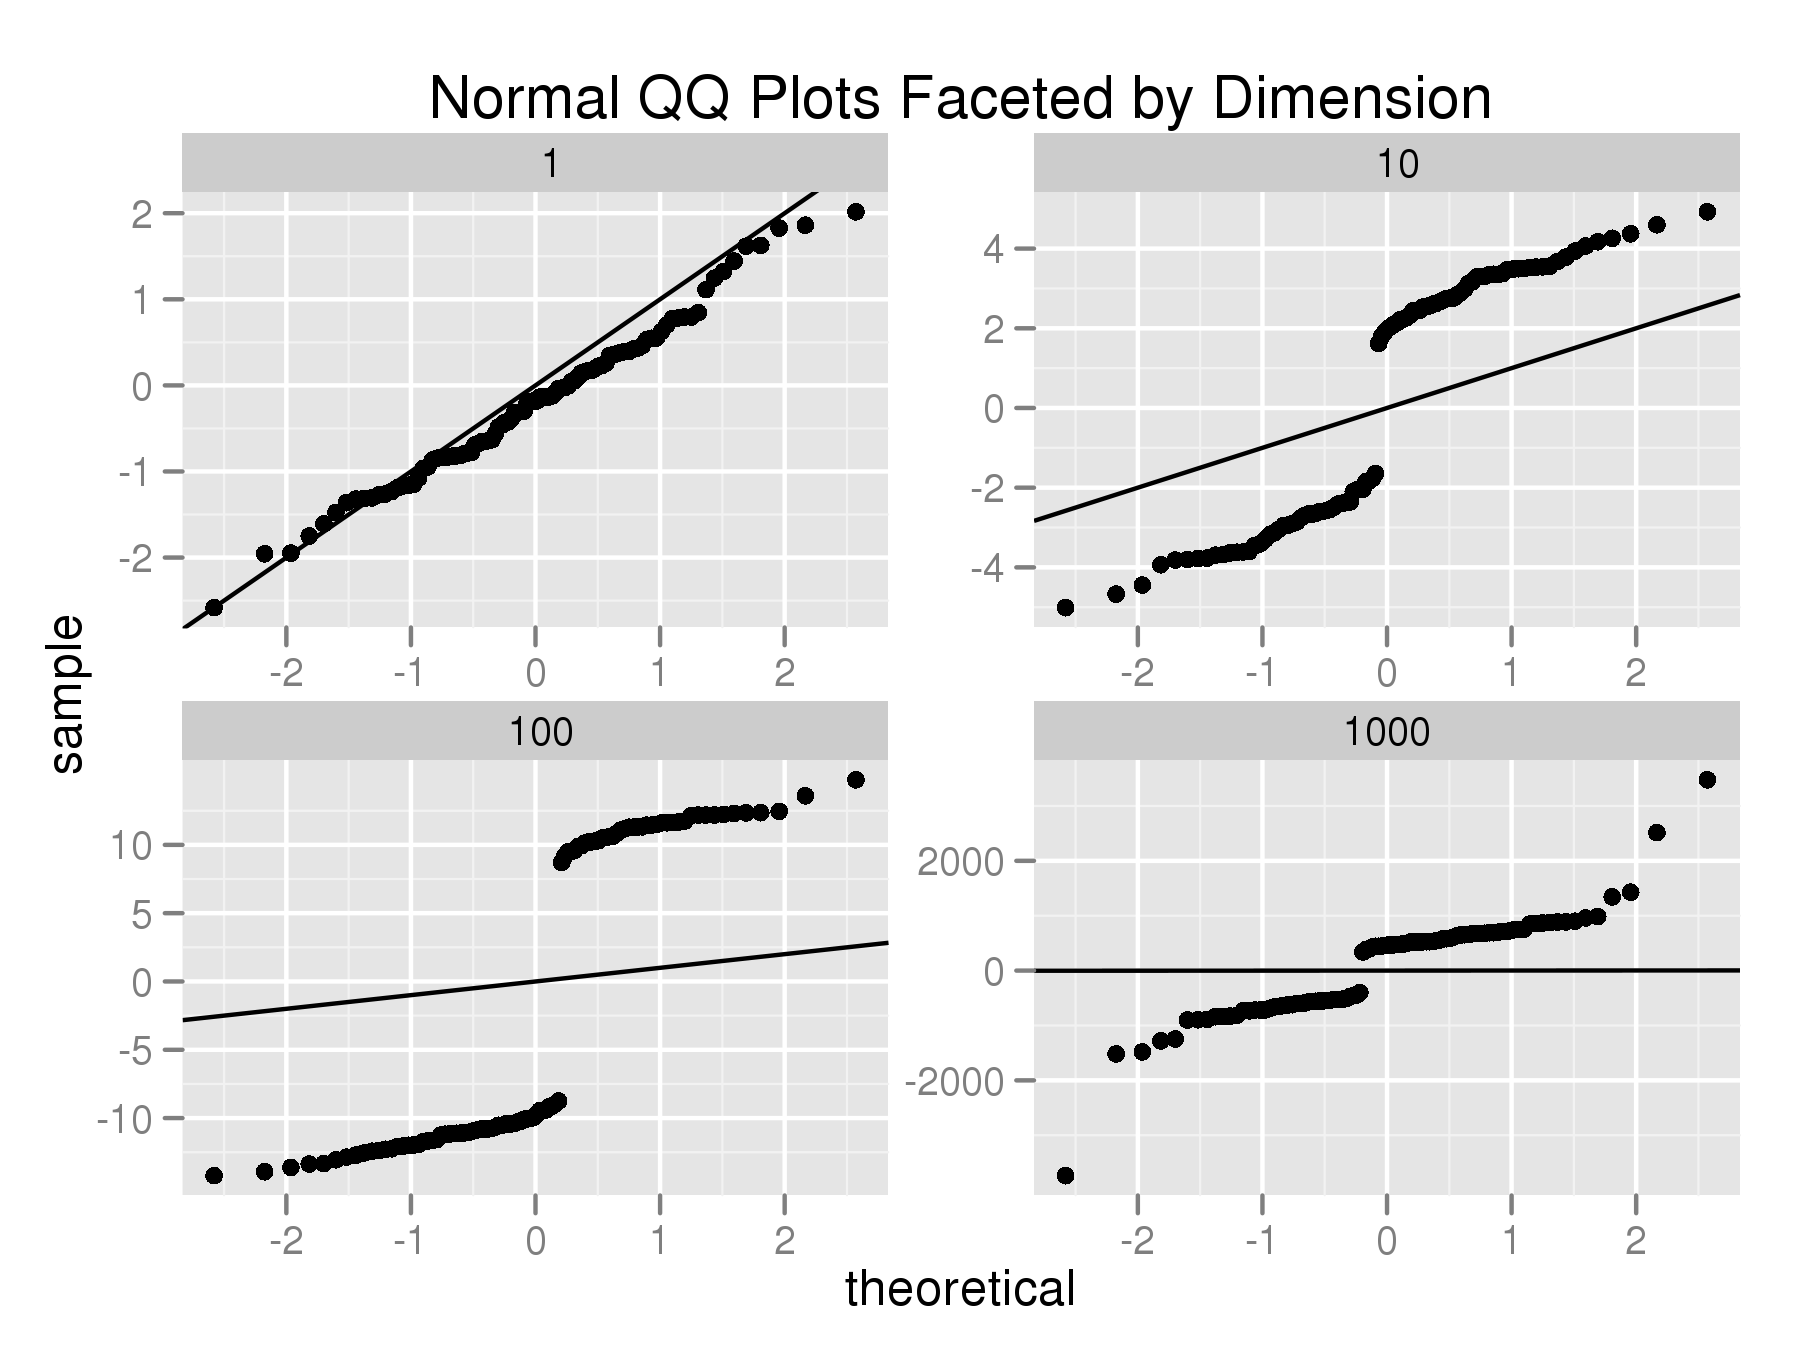
\includegraphics{./simulations/ARC/multivar_qq.png}
\end{figure}

At a sample size of 100 and with univariate data, the standard Normal
is a close fit.  With increasing dimensionality, the Friedman
statistic gets more and more extreme.  One possible explanation is
that it becomes easier to separate two sets of points as the
dimensionality increases.
\clearpage

Here we look at univariate data but with an inhomogeneous kernel
($k(x, x') = (<x,x'>+1)^d$) of degree $d$:
\begin{figure}[!ht]
  \centering
  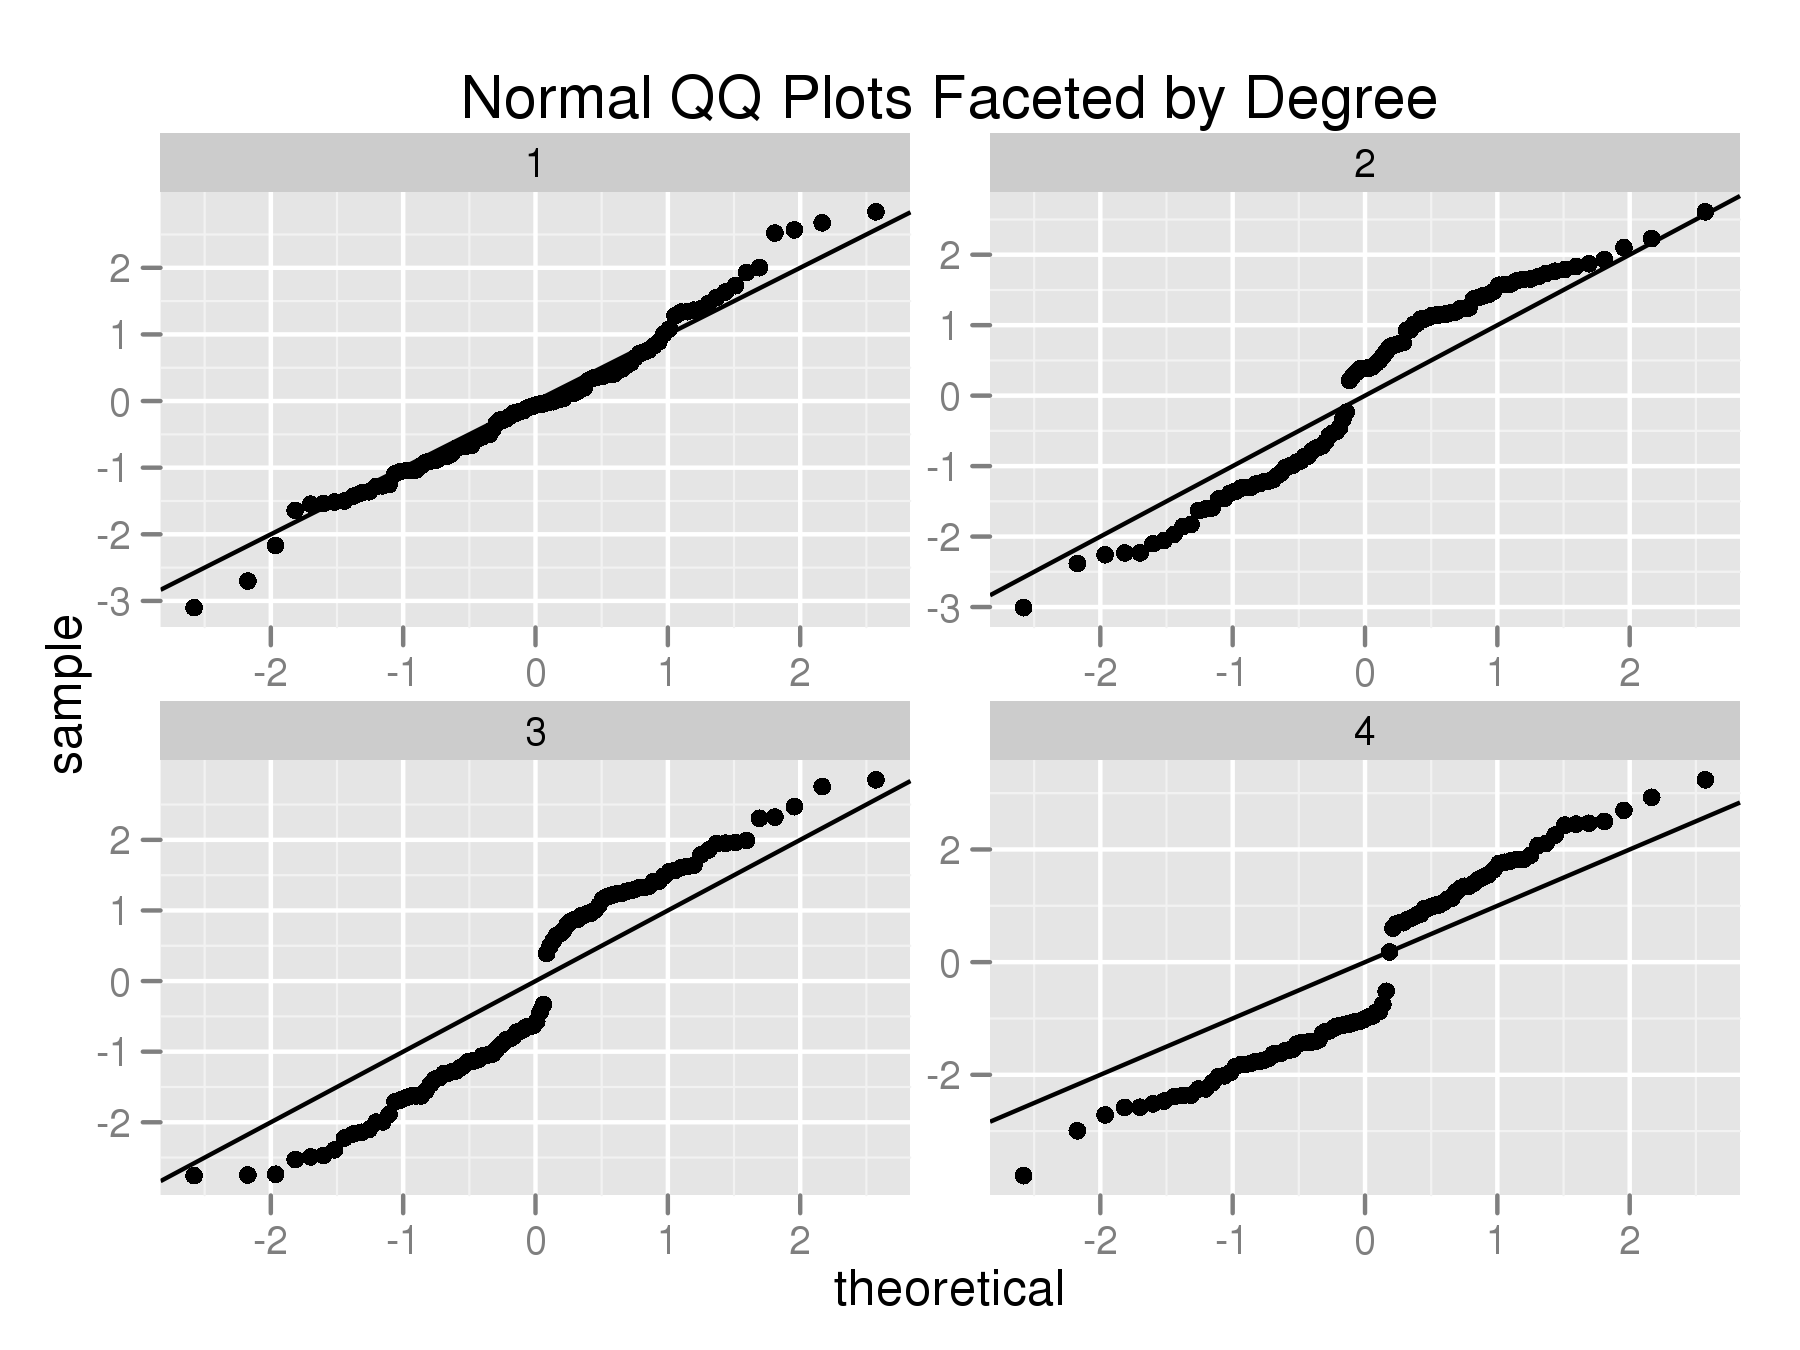
\includegraphics{./simulations/ARC/poly_ker_qq.png}
\end{figure}

The polynomial kernel for degrees greater than 1 yields null
distributions with fatter tails than the standard Normal.
\clearpage

Here we look at the effects of both dimension of the underlying data
and degree of the inhomogeneous kernel:
\begin{figure}[!ht]
  \centering
  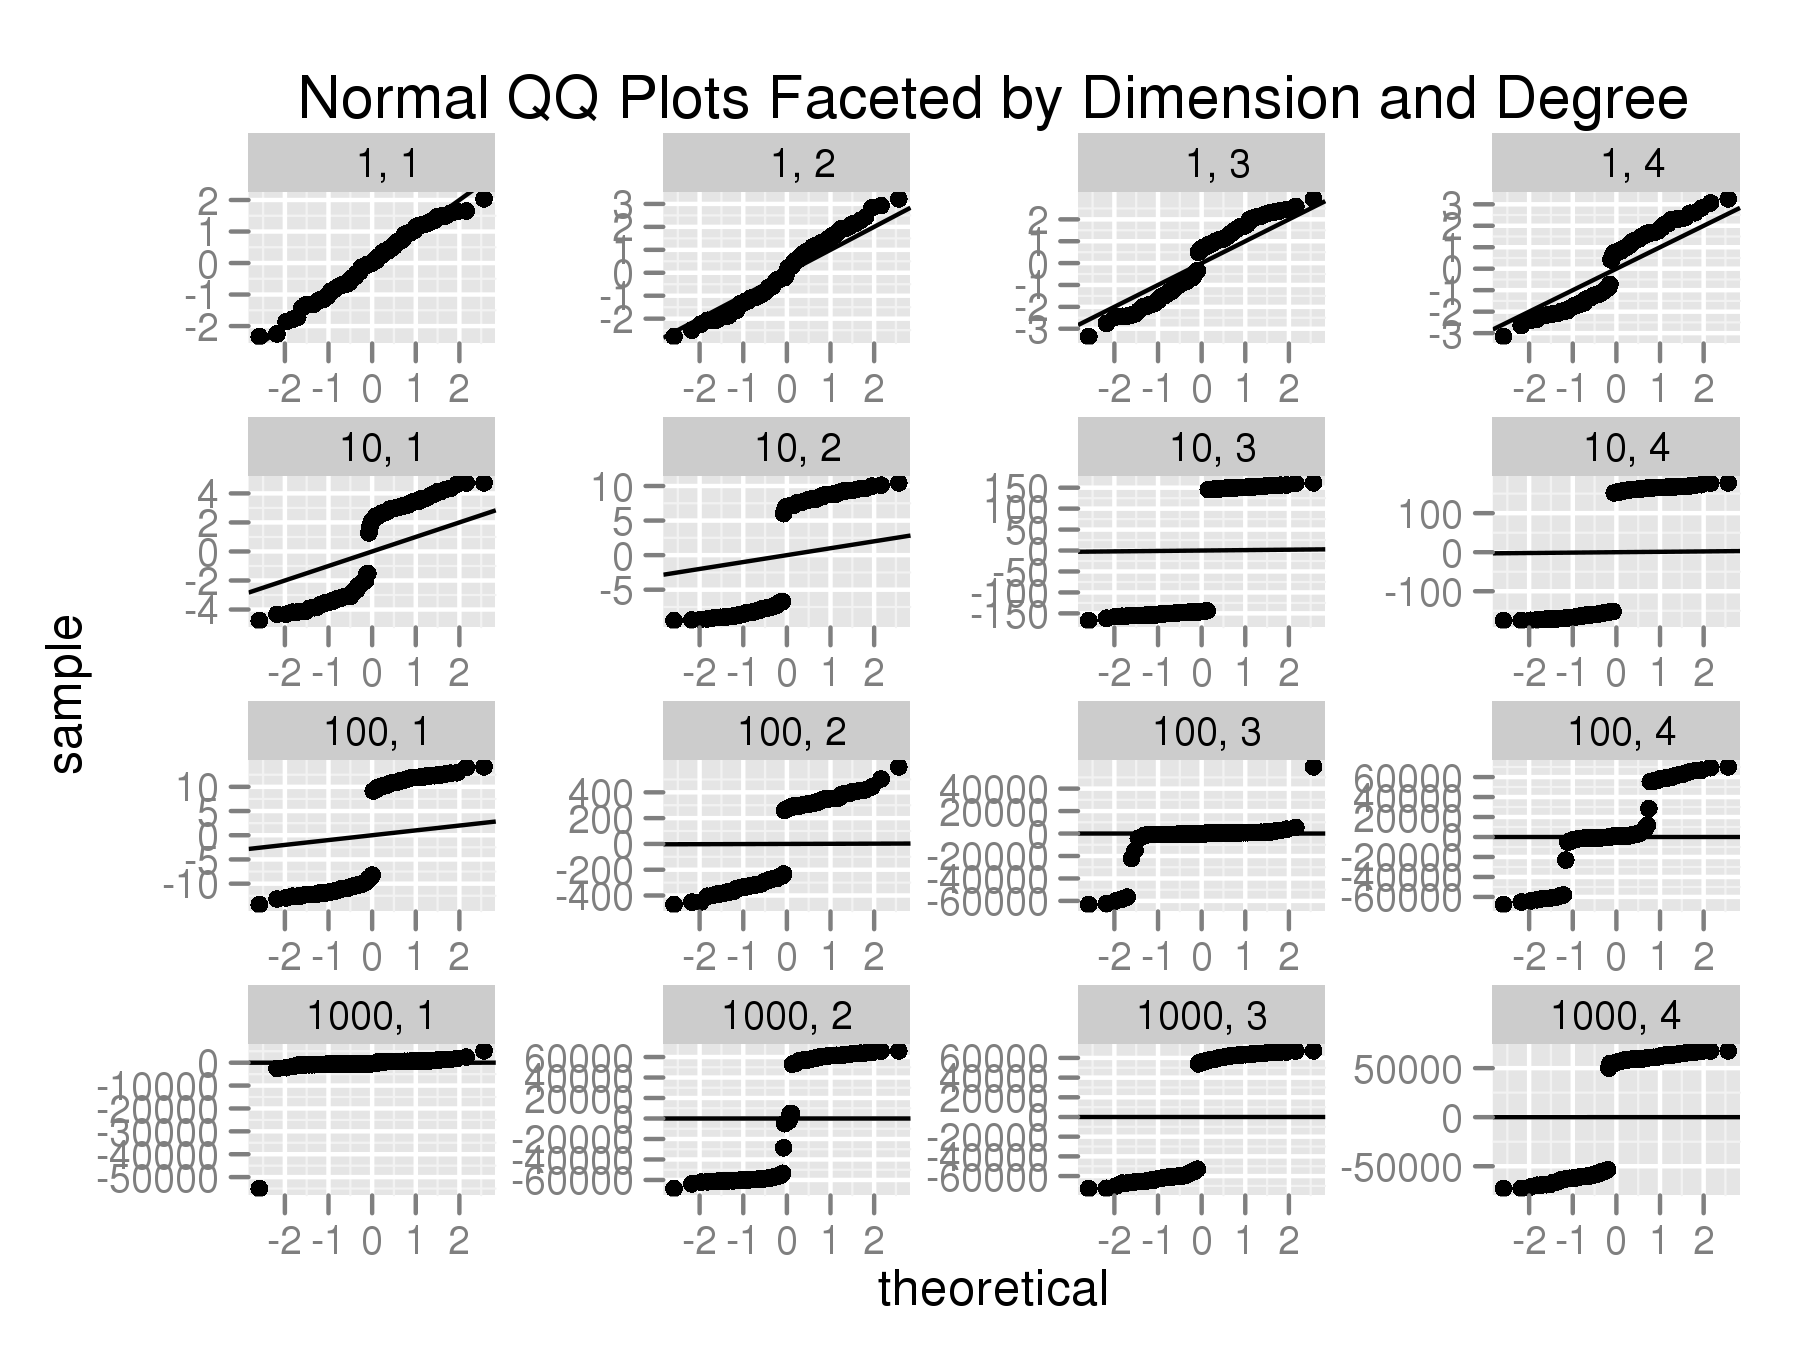
\includegraphics{./simulations/ARC/multivar_poly_ker_qq.png}
\end{figure}
\clearpage

\section{Generalizations (Approximate Regression Condition)}
Here we plot $T'$ on $T$, where $T'$ results from swapping labels and
refitting the SVM.  Note that here we don't assign the statistics
random signs because there is no clear way to maintain the coupling
between $T$ and $T'$.

The dimensions (rows) are 1, 10, and 100, and the sample sizes
(columns) are 10, 100, and 1000.
\begin{figure}[!ht]
  \centering
  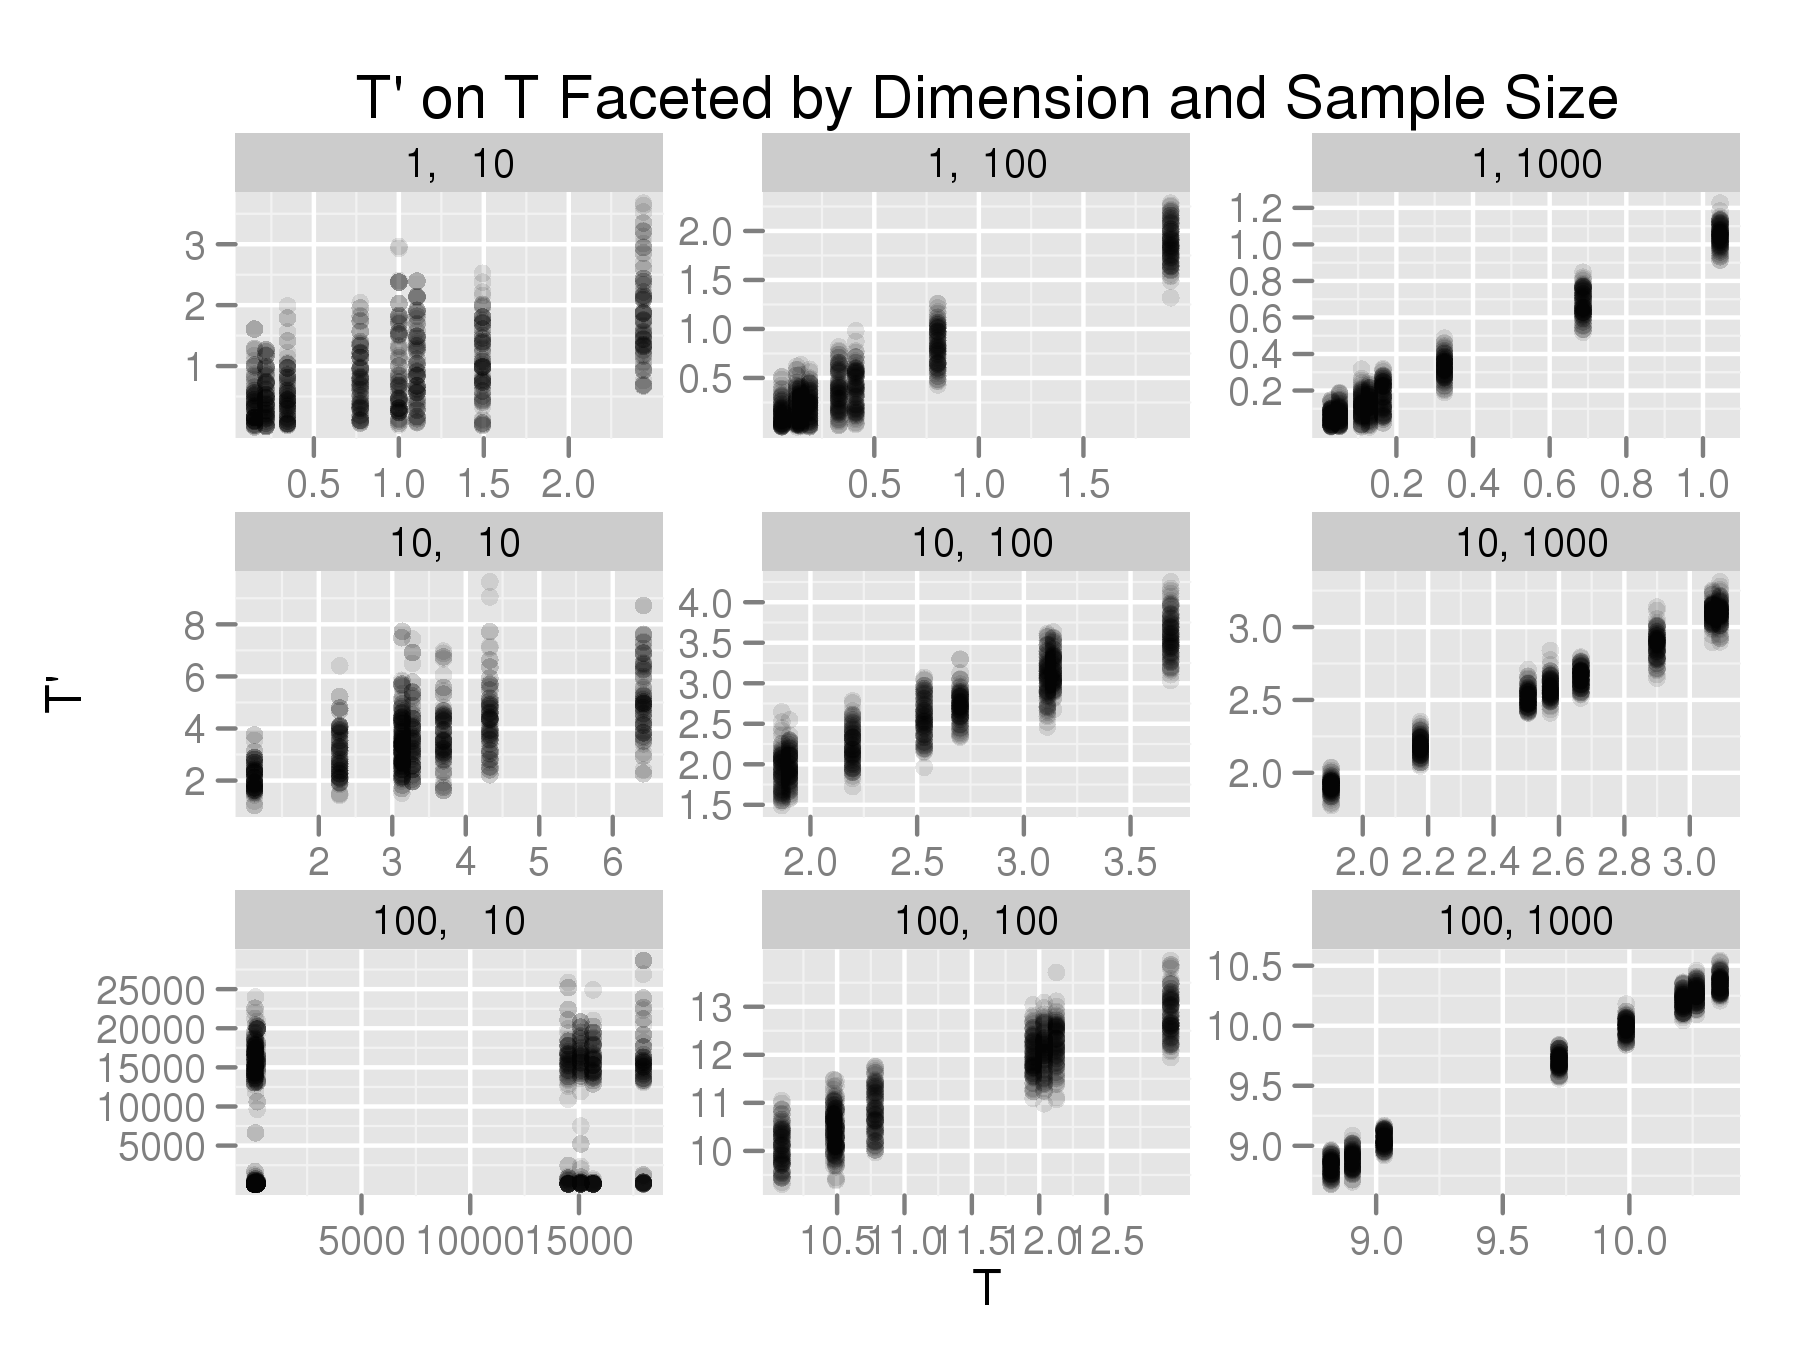
\includegraphics{./simulations/ARC/multivar_ARC.png}
\end{figure}

Across a row, it is clear that a larger sample size decreases the
variability of $T'$ about $T$.  And down a column, it is clear that
increasing dimensionality results in a greater departure from (folded)
Normality.  It is not clear whether the reduction in variability is of
order $1/N$.
\clearpage

Here we look at sample sizes (columns) of 10, 100, and 200 and
inhomogeneous polynomial kernel degrees (rows) of 1, 2, and 5.
\begin{figure}[!ht]
  \centering
  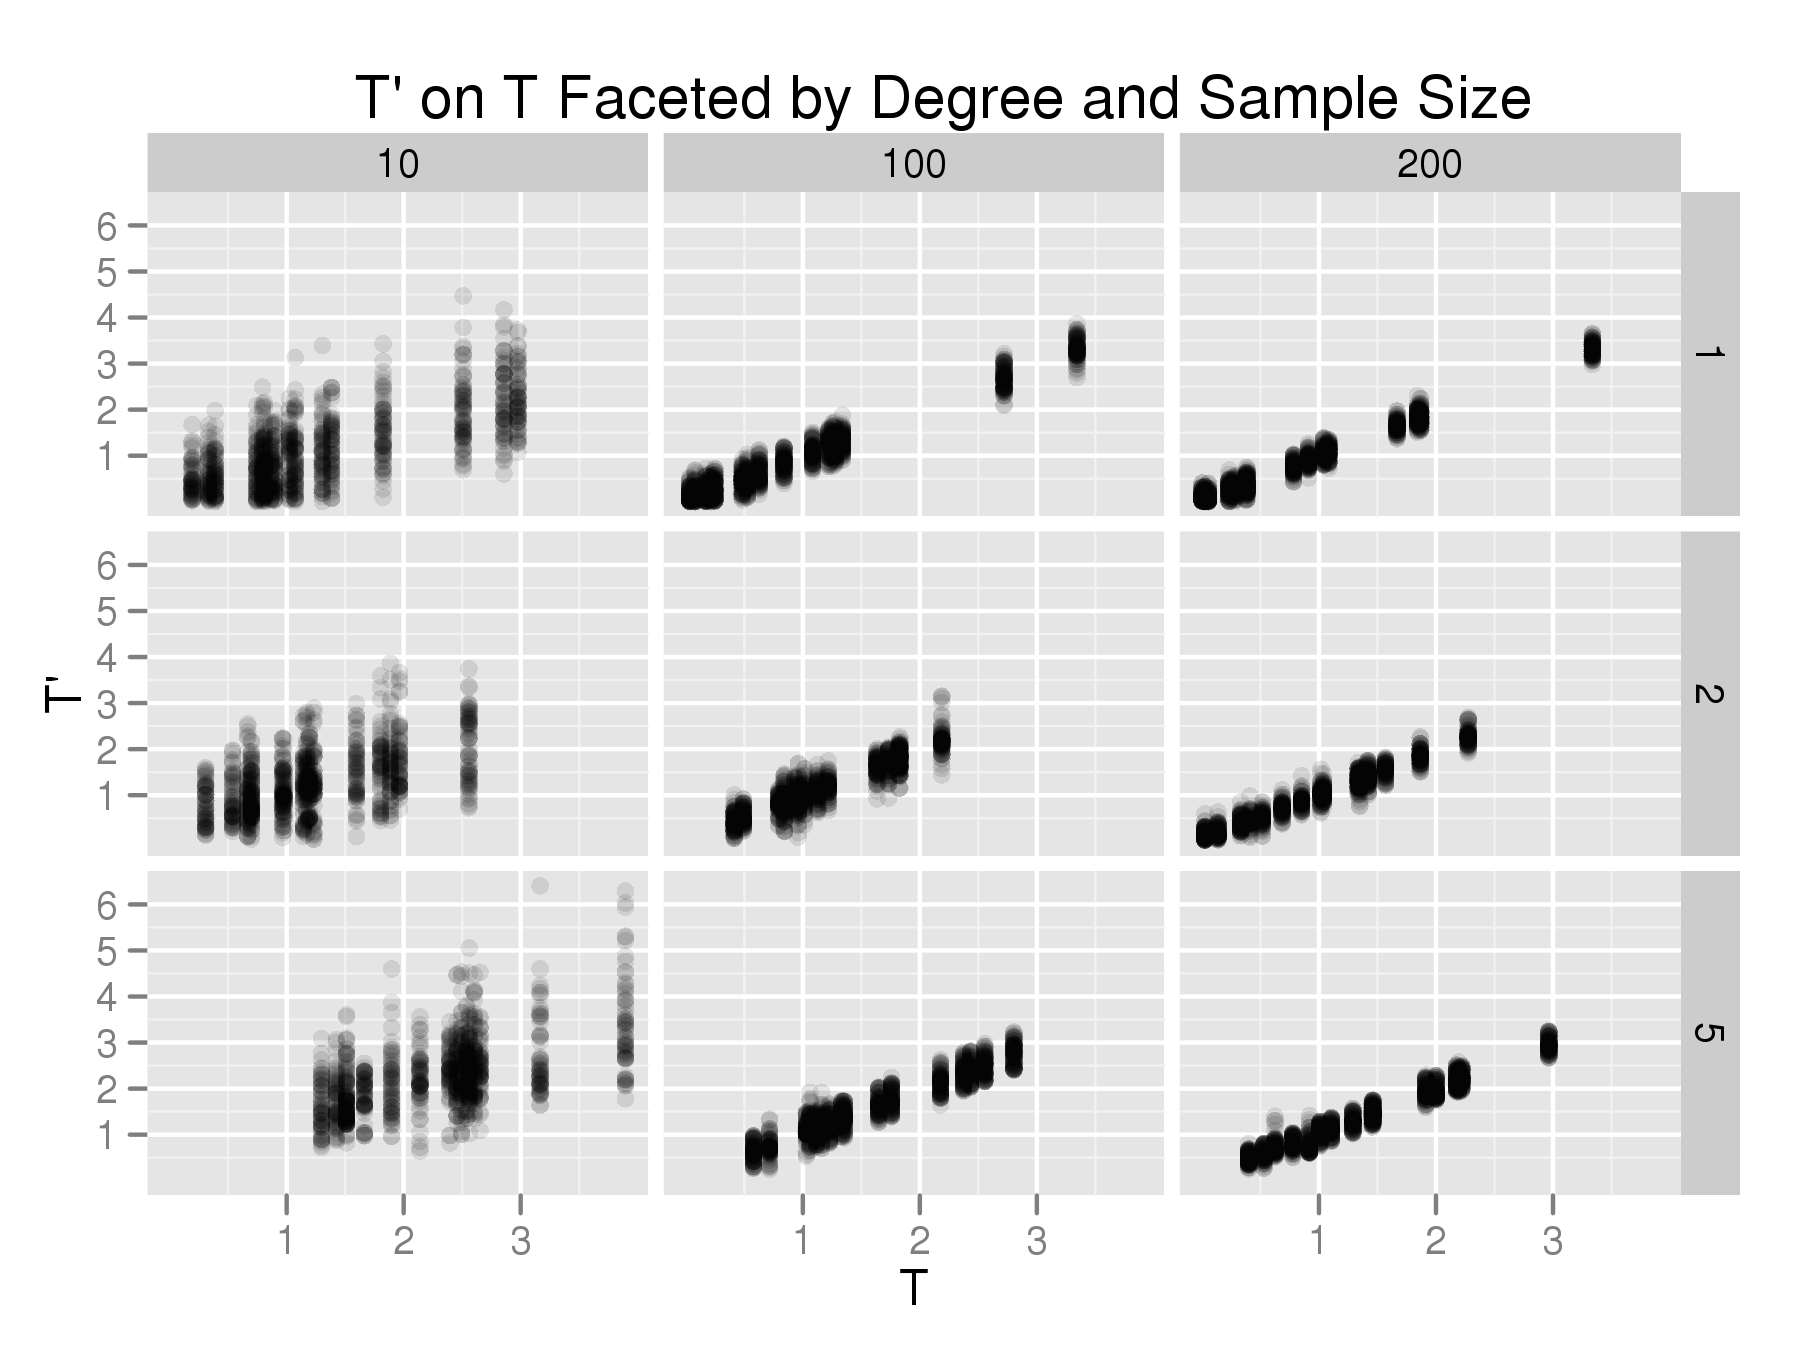
\includegraphics{./simulations/ARC/poly_ker_ARC.png}
\end{figure}

We again observe an approximately linear plus noise relationship
between $T'$ and $T$ with the noise decreasing in sample size.  
